\documentclass[twoside]{book}

% Packages required by doxygen
\usepackage{calc}
\usepackage{doxygen}
\usepackage{graphicx}
\usepackage[utf8]{inputenc}
\usepackage{makeidx}
\usepackage{multicol}
\usepackage{multirow}
\usepackage{textcomp}
\usepackage[table]{xcolor}

% NLS support packages
\usepackage[ngerman]{babel}

% Font selection
\usepackage[T1]{fontenc}
\usepackage{mathptmx}
\usepackage[scaled=.90]{helvet}
\usepackage{courier}
\usepackage{amssymb}
\usepackage{sectsty}
\renewcommand{\familydefault}{\sfdefault}
\allsectionsfont{%
  \fontseries{bc}\selectfont%
  \color{darkgray}%
}
\renewcommand{\DoxyLabelFont}{%
  \fontseries{bc}\selectfont%
  \color{darkgray}%
}

% Page & text layout
\usepackage{geometry}
\geometry{%
  a4paper,%
  top=2.5cm,%
  bottom=2.5cm,%
  left=2.5cm,%
  right=2.5cm%
}
\tolerance=750
\hfuzz=15pt
\hbadness=750
\setlength{\emergencystretch}{15pt}
\setlength{\parindent}{0cm}
\setlength{\parskip}{0.2cm}
\makeatletter
\renewcommand{\paragraph}{%
  \@startsection{paragraph}{4}{0ex}{-1.0ex}{1.0ex}{%
    \normalfont\normalsize\bfseries\SS@parafont%
  }%
}
\renewcommand{\subparagraph}{%
  \@startsection{subparagraph}{5}{0ex}{-1.0ex}{1.0ex}{%
    \normalfont\normalsize\bfseries\SS@subparafont%
  }%
}
\makeatother

% Headers & footers
\usepackage{fancyhdr}
\pagestyle{fancyplain}
\fancyhead[LE]{\fancyplain{}{\bfseries\thepage}}
\fancyhead[CE]{\fancyplain{}{}}
\fancyhead[RE]{\fancyplain{}{\bfseries\leftmark}}
\fancyhead[LO]{\fancyplain{}{\bfseries\rightmark}}
\fancyhead[CO]{\fancyplain{}{}}
\fancyhead[RO]{\fancyplain{}{\bfseries\thepage}}
\fancyfoot[LE]{\fancyplain{}{}}
\fancyfoot[CE]{\fancyplain{}{}}
\fancyfoot[RE]{\fancyplain{}{\bfseries\scriptsize Erzeugt am Mon Jun 24 2013 21:50:40 für Dungeon Crawler 2013 von Doxygen }}
\fancyfoot[LO]{\fancyplain{}{\bfseries\scriptsize Erzeugt am Mon Jun 24 2013 21:50:40 für Dungeon Crawler 2013 von Doxygen }}
\fancyfoot[CO]{\fancyplain{}{}}
\fancyfoot[RO]{\fancyplain{}{}}
\renewcommand{\footrulewidth}{0.4pt}
\renewcommand{\chaptermark}[1]{%
  \markboth{#1}{}%
}
\renewcommand{\sectionmark}[1]{%
  \markright{\thesection\ #1}%
}

% Indices & bibliography
\usepackage{natbib}
\usepackage[titles]{tocloft}
\setcounter{tocdepth}{3}
\setcounter{secnumdepth}{5}
\makeindex

% Hyperlinks (required, but should be loaded last)
\usepackage{ifpdf}
\ifpdf
  \usepackage[pdftex,pagebackref=true]{hyperref}
\else
  \usepackage[ps2pdf,pagebackref=true]{hyperref}
\fi
\hypersetup{%
  colorlinks=true,%
  linkcolor=blue,%
  citecolor=blue,%
  unicode%
}

% Custom commands
\newcommand{\clearemptydoublepage}{%
  \newpage{\pagestyle{empty}\cleardoublepage}%
}


%===== C O N T E N T S =====

\begin{document}

% Titlepage & ToC
\hypersetup{pageanchor=false}
\pagenumbering{roman}
\begin{titlepage}
\vspace*{7cm}
\begin{center}%
{\Large Dungeon Crawler 2013 \\[1ex]\large 0.\-2 }\\
\vspace*{1cm}
{\large Erzeugt von Doxygen 1.8.4}\\
\vspace*{0.5cm}
{\small Mon Jun 24 2013 21:50:40}\\
\end{center}
\end{titlepage}
\clearemptydoublepage
\tableofcontents
\clearemptydoublepage
\pagenumbering{arabic}
\hypersetup{pageanchor=true}

%--- Begin generated contents ---
\chapter{Verzeichnis der Namensbereiche}
\section{Pakete}
Hier folgen die Pakete mit einer Kurzbeschreibung (wenn verfügbar)\-:\begin{DoxyCompactList}
\item\contentsline{section}{\hyperlink{namespace_dungeon_server}{Dungeon\-Server} }{\pageref{namespace_dungeon_server}}{}
\item\contentsline{section}{\hyperlink{namespace_gruppe22}{Gruppe22} }{\pageref{namespace_gruppe22}}{}
\item\contentsline{section}{\hyperlink{namespace_gruppe22_1_1_backend}{Gruppe22.\-Backend} }{\pageref{namespace_gruppe22_1_1_backend}}{}
\item\contentsline{section}{\hyperlink{namespace_gruppe22_1_1_client}{Gruppe22.\-Client} }{\pageref{namespace_gruppe22_1_1_client}}{}
\end{DoxyCompactList}

\chapter{Hierarchie-\/\-Verzeichnis}
\section{Klassenhierarchie}
Die Liste der Ableitungen ist -\/mit Einschränkungen-\/ alphabetisch sortiert\-:\begin{DoxyCompactList}
\item \contentsline{section}{Gruppe22.\-Backend.\-Ability}{\pageref{class_gruppe22_1_1_backend_1_1_ability}}{}
\item \contentsline{section}{Gruppe22.\-Backend.\-Actor}{\pageref{class_gruppe22_1_1_backend_1_1_actor}}{}
\begin{DoxyCompactList}
\item \contentsline{section}{Gruppe22.\-Backend.\-Enemy}{\pageref{class_gruppe22_1_1_backend_1_1_enemy}}{}
\item \contentsline{section}{Gruppe22.\-Backend.\-N\-P\-C}{\pageref{class_gruppe22_1_1_backend_1_1_n_p_c}}{}
\item \contentsline{section}{Gruppe22.\-Backend.\-Player}{\pageref{class_gruppe22_1_1_backend_1_1_player}}{}
\end{DoxyCompactList}
\item \contentsline{section}{Gruppe22.\-Client.\-Camera}{\pageref{class_gruppe22_1_1_client_1_1_camera}}{}
\item \contentsline{section}{Dungeon\-Server.\-Client\-Data}{\pageref{class_dungeon_server_1_1_client_data}}{}
\item \contentsline{section}{Gruppe22.\-Client.\-Client\-Data}{\pageref{class_gruppe22_1_1_client_1_1_client_data}}{}
\item \contentsline{section}{Gruppe22.\-Client.\-Create\-X\-M\-L\-Files}{\pageref{class_gruppe22_1_1_client_1_1_create_x_m_l_files}}{}
\item \contentsline{section}{Gruppe22.\-Backend.\-Exit}{\pageref{class_gruppe22_1_1_backend_1_1_exit}}{}
\item \contentsline{section}{Gruppe22.\-Client.\-Float\-Number}{\pageref{class_gruppe22_1_1_client_1_1_float_number}}{}
\item Game\begin{DoxyCompactList}
\item \contentsline{section}{Gruppe22.\-Client.\-Game\-Win}{\pageref{class_gruppe22_1_1_client_1_1_game_win}}{}
\begin{DoxyCompactList}
\item \contentsline{section}{Gruppe22.\-Backend.\-Game\-Logic}{\pageref{class_gruppe22_1_1_backend_1_1_game_logic}}{}
\begin{DoxyCompactList}
\item \contentsline{section}{Gruppe22.\-Main\-Window}{\pageref{class_gruppe22_1_1_main_window}}{}
\end{DoxyCompactList}
\end{DoxyCompactList}
\end{DoxyCompactList}
\item \contentsline{section}{Gruppe22.\-Client.\-Grid\-Element}{\pageref{class_gruppe22_1_1_client_1_1_grid_element}}{}
\item I\-Comparable$<$ Coords $>$\begin{DoxyCompactList}
\item \contentsline{section}{Gruppe22.\-Backend.\-Coords}{\pageref{class_gruppe22_1_1_backend_1_1_coords}}{}
\begin{DoxyCompactList}
\item \contentsline{section}{Gruppe22.\-Backend.\-Path}{\pageref{class_gruppe22_1_1_backend_1_1_path}}{}
\end{DoxyCompactList}
\end{DoxyCompactList}
\item I\-Comparable$<$ Int32 $>$\begin{DoxyCompactList}
\item \contentsline{section}{Gruppe22.\-Backend.\-Coords}{\pageref{class_gruppe22_1_1_backend_1_1_coords}}{}
\end{DoxyCompactList}
\item I\-Disposable\begin{DoxyCompactList}
\item \contentsline{section}{Gruppe22.\-Backend.\-Floor\-Tile}{\pageref{class_gruppe22_1_1_backend_1_1_floor_tile}}{}
\begin{DoxyCompactList}
\item \contentsline{section}{Gruppe22.\-Backend.\-Generator\-Tile}{\pageref{class_gruppe22_1_1_backend_1_1_generator_tile}}{}
\end{DoxyCompactList}
\item \contentsline{section}{Gruppe22.\-Backend.\-Map}{\pageref{class_gruppe22_1_1_backend_1_1_map}}{}
\begin{DoxyCompactList}
\item \contentsline{section}{Gruppe22.\-Backend.\-Generator}{\pageref{class_gruppe22_1_1_backend_1_1_generator}}{}
\end{DoxyCompactList}
\item \contentsline{section}{Gruppe22.\-Client.\-Button}{\pageref{class_gruppe22_1_1_client_1_1_button}}{}
\item \contentsline{section}{Gruppe22.\-Client.\-U\-I\-Element}{\pageref{class_gruppe22_1_1_client_1_1_u_i_element}}{}
\begin{DoxyCompactList}
\item \contentsline{section}{Gruppe22.\-Client.\-Button}{\pageref{class_gruppe22_1_1_client_1_1_button}}{}
\item \contentsline{section}{Gruppe22.\-Client.\-Grid}{\pageref{class_gruppe22_1_1_client_1_1_grid}}{}
\begin{DoxyCompactList}
\item \contentsline{section}{Gruppe22.\-Client.\-Abilities}{\pageref{class_gruppe22_1_1_client_1_1_abilities}}{}
\item \contentsline{section}{Gruppe22.\-Client.\-Ability\-Choice}{\pageref{class_gruppe22_1_1_client_1_1_ability_choice}}{}
\item \contentsline{section}{Gruppe22.\-Client.\-Inventory}{\pageref{class_gruppe22_1_1_client_1_1_inventory}}{}
\end{DoxyCompactList}
\item \contentsline{section}{Gruppe22.\-Client.\-Menu}{\pageref{class_gruppe22_1_1_client_1_1_menu}}{}
\item \contentsline{section}{Gruppe22.\-Client.\-Orb}{\pageref{class_gruppe22_1_1_client_1_1_orb}}{}
\item \contentsline{section}{Gruppe22.\-Client.\-Progress\-Bar}{\pageref{class_gruppe22_1_1_client_1_1_progress_bar}}{}
\item \contentsline{section}{Gruppe22.\-Client.\-Simple\-Stats}{\pageref{class_gruppe22_1_1_client_1_1_simple_stats}}{}
\item \contentsline{section}{Gruppe22.\-Client.\-Text\-Input}{\pageref{class_gruppe22_1_1_client_1_1_text_input}}{}
\begin{DoxyCompactList}
\item \contentsline{section}{Gruppe22.\-Client.\-Number\-Entry}{\pageref{class_gruppe22_1_1_client_1_1_number_entry}}{}
\end{DoxyCompactList}
\item \contentsline{section}{Gruppe22.\-Client.\-Text\-Output}{\pageref{class_gruppe22_1_1_client_1_1_text_output}}{}
\begin{DoxyCompactList}
\item \contentsline{section}{Gruppe22.\-Client.\-Chat}{\pageref{class_gruppe22_1_1_client_1_1_chat}}{}
\item \contentsline{section}{Gruppe22.\-Client.\-Statusbox}{\pageref{class_gruppe22_1_1_client_1_1_statusbox}}{}
\end{DoxyCompactList}
\item \contentsline{section}{Gruppe22.\-Client.\-Toolbar}{\pageref{class_gruppe22_1_1_client_1_1_toolbar}}{}
\item \contentsline{section}{Gruppe22.\-Client.\-Window}{\pageref{class_gruppe22_1_1_client_1_1_window}}{}
\begin{DoxyCompactList}
\item \contentsline{section}{Gruppe22.\-Client.\-Character\-Window}{\pageref{class_gruppe22_1_1_client_1_1_character_window}}{}
\item \contentsline{section}{Gruppe22.\-Client.\-Dialog}{\pageref{class_gruppe22_1_1_client_1_1_dialog}}{}
\item \contentsline{section}{Gruppe22.\-Client.\-File\-Dialog}{\pageref{class_gruppe22_1_1_client_1_1_file_dialog}}{}
\item \contentsline{section}{Gruppe22.\-Client.\-Lobby}{\pageref{class_gruppe22_1_1_client_1_1_lobby}}{}
\item \contentsline{section}{Gruppe22.\-Client.\-Modify\-Window}{\pageref{class_gruppe22_1_1_client_1_1_modify_window}}{}
\item \contentsline{section}{Gruppe22.\-Client.\-Shop}{\pageref{class_gruppe22_1_1_client_1_1_shop}}{}
\end{DoxyCompactList}
\item \contentsline{section}{Gruppe22.\-Client.\-Zoomable}{\pageref{class_gruppe22_1_1_client_1_1_zoomable}}{}
\begin{DoxyCompactList}
\item \contentsline{section}{Gruppe22.\-Client.\-Mainmap}{\pageref{class_gruppe22_1_1_client_1_1_mainmap}}{}
\item \contentsline{section}{Gruppe22.\-Client.\-Minimap}{\pageref{class_gruppe22_1_1_client_1_1_minimap}}{}
\end{DoxyCompactList}
\end{DoxyCompactList}
\end{DoxyCompactList}
\item I\-Equatable$<$ Coords $>$\begin{DoxyCompactList}
\item \contentsline{section}{Gruppe22.\-Backend.\-Coords}{\pageref{class_gruppe22_1_1_backend_1_1_coords}}{}
\end{DoxyCompactList}
\item \contentsline{section}{Gruppe22.\-Backend.\-I\-Handle\-Event}{\pageref{interface_gruppe22_1_1_backend_1_1_i_handle_event}}{}
\begin{DoxyCompactList}
\item \contentsline{section}{Gruppe22.\-Backend.\-Map}{\pageref{class_gruppe22_1_1_backend_1_1_map}}{}
\item \contentsline{section}{Gruppe22.\-Backend.\-Tile}{\pageref{class_gruppe22_1_1_backend_1_1_tile}}{}
\begin{DoxyCompactList}
\item \contentsline{section}{Gruppe22.\-Backend.\-Actor\-Tile}{\pageref{class_gruppe22_1_1_backend_1_1_actor_tile}}{}
\item \contentsline{section}{Gruppe22.\-Backend.\-Bomb\-Tile}{\pageref{class_gruppe22_1_1_backend_1_1_bomb_tile}}{}
\item \contentsline{section}{Gruppe22.\-Backend.\-Checkpoint\-Tile}{\pageref{class_gruppe22_1_1_backend_1_1_checkpoint_tile}}{}
\item \contentsline{section}{Gruppe22.\-Backend.\-Floor\-Tile}{\pageref{class_gruppe22_1_1_backend_1_1_floor_tile}}{}
\item \contentsline{section}{Gruppe22.\-Backend.\-Gap\-Tile}{\pageref{class_gruppe22_1_1_backend_1_1_gap_tile}}{}
\item \contentsline{section}{Gruppe22.\-Backend.\-Item\-Tile}{\pageref{class_gruppe22_1_1_backend_1_1_item_tile}}{}
\item \contentsline{section}{Gruppe22.\-Backend.\-Reserved\-Tile}{\pageref{class_gruppe22_1_1_backend_1_1_reserved_tile}}{}
\item \contentsline{section}{Gruppe22.\-Backend.\-Switch\-Tile}{\pageref{class_gruppe22_1_1_backend_1_1_switch_tile}}{}
\item \contentsline{section}{Gruppe22.\-Backend.\-Target\-Tile}{\pageref{class_gruppe22_1_1_backend_1_1_target_tile}}{}
\item \contentsline{section}{Gruppe22.\-Backend.\-Teleport\-Tile}{\pageref{class_gruppe22_1_1_backend_1_1_teleport_tile}}{}
\item \contentsline{section}{Gruppe22.\-Backend.\-Trap\-Tile}{\pageref{class_gruppe22_1_1_backend_1_1_trap_tile}}{}
\item \contentsline{section}{Gruppe22.\-Backend.\-Trigger\-Tile}{\pageref{class_gruppe22_1_1_backend_1_1_trigger_tile}}{}
\item \contentsline{section}{Gruppe22.\-Backend.\-Wall\-Tile}{\pageref{class_gruppe22_1_1_backend_1_1_wall_tile}}{}
\begin{DoxyCompactList}
\item \contentsline{section}{Gruppe22.\-Backend.\-Door\-Tile}{\pageref{class_gruppe22_1_1_backend_1_1_door_tile}}{}
\end{DoxyCompactList}
\item \contentsline{section}{Gruppe22.\-Projectile\-Tile}{\pageref{class_gruppe22_1_1_projectile_tile}}{}
\end{DoxyCompactList}
\item \contentsline{section}{Gruppe22.\-Client.\-Game\-Win}{\pageref{class_gruppe22_1_1_client_1_1_game_win}}{}
\item \contentsline{section}{Gruppe22.\-Client.\-Number\-Entry}{\pageref{class_gruppe22_1_1_client_1_1_number_entry}}{}
\item \contentsline{section}{Gruppe22.\-Client.\-Progress\-Bar}{\pageref{class_gruppe22_1_1_client_1_1_progress_bar}}{}
\item \contentsline{section}{Gruppe22.\-Client.\-Simple\-Stats}{\pageref{class_gruppe22_1_1_client_1_1_simple_stats}}{}
\item \contentsline{section}{Gruppe22.\-Client.\-Text\-Output}{\pageref{class_gruppe22_1_1_client_1_1_text_output}}{}
\item \contentsline{section}{Gruppe22.\-Client.\-U\-I\-Element}{\pageref{class_gruppe22_1_1_client_1_1_u_i_element}}{}
\end{DoxyCompactList}
\item \contentsline{section}{Gruppe22.\-Client.\-I\-Key\-Handler}{\pageref{interface_gruppe22_1_1_client_1_1_i_key_handler}}{}
\begin{DoxyCompactList}
\item \contentsline{section}{Gruppe22.\-Client.\-Game\-Win}{\pageref{class_gruppe22_1_1_client_1_1_game_win}}{}
\item \contentsline{section}{Gruppe22.\-Client.\-U\-I\-Element}{\pageref{class_gruppe22_1_1_client_1_1_u_i_element}}{}
\end{DoxyCompactList}
\item \contentsline{section}{Gruppe22.\-Backend.\-Image\-Data}{\pageref{class_gruppe22_1_1_backend_1_1_image_data}}{}
\item \contentsline{section}{Gruppe22.\-Backend.\-Item}{\pageref{class_gruppe22_1_1_backend_1_1_item}}{}
\item \contentsline{section}{Gruppe22.\-Backend.\-Item\-Effect}{\pageref{class_gruppe22_1_1_backend_1_1_item_effect}}{}
\item I\-Xml\-Serializable\begin{DoxyCompactList}
\item \contentsline{section}{Gruppe22.\-Client.\-Tile\-Object}{\pageref{class_gruppe22_1_1_client_1_1_tile_object}}{}
\item \contentsline{section}{Gruppe22.\-Client.\-Tile\-Set}{\pageref{class_gruppe22_1_1_client_1_1_tile_set}}{}
\begin{DoxyCompactList}
\item \contentsline{section}{Gruppe22.\-Client.\-Actor\-View}{\pageref{class_gruppe22_1_1_client_1_1_actor_view}}{}
\item \contentsline{section}{Gruppe22.\-Client.\-Wall\-Tiles}{\pageref{class_gruppe22_1_1_client_1_1_wall_tiles}}{}
\end{DoxyCompactList}
\item \contentsline{section}{Gruppe22.\-Client.\-Visible\-Object}{\pageref{class_gruppe22_1_1_client_1_1_visible_object}}{}
\end{DoxyCompactList}
\item \contentsline{section}{Gruppe22.\-Client.\-Map\-Effect}{\pageref{class_gruppe22_1_1_client_1_1_map_effect}}{}
\item \contentsline{section}{Gruppe22.\-Backend.\-Movable\-Tile}{\pageref{class_gruppe22_1_1_backend_1_1_movable_tile}}{}
\item \contentsline{section}{Gruppe22.\-Client.\-Net\-Player}{\pageref{class_gruppe22_1_1_client_1_1_net_player}}{}
\item \contentsline{section}{Gruppe22.\-Client.\-Projectile}{\pageref{class_gruppe22_1_1_client_1_1_projectile}}{}
\item \contentsline{section}{Dungeon\-Server.\-Server}{\pageref{class_dungeon_server_1_1_server}}{}
\item \contentsline{section}{Gruppe22.\-Client.\-State\-To\-Event}{\pageref{class_gruppe22_1_1_client_1_1_state_to_event}}{}
\item \contentsline{section}{Gruppe22.\-Client.\-Texture\-From\-Data}{\pageref{class_gruppe22_1_1_client_1_1_texture_from_data}}{}
\item \contentsline{section}{Gruppe22.\-Client.\-Tile\-Tooltip}{\pageref{class_gruppe22_1_1_client_1_1_tile_tooltip}}{}
\end{DoxyCompactList}

\chapter{Klassen-\/\-Verzeichnis}
\section{Auflistung der Klassen}
Hier folgt die Aufzählung aller Klassen, Strukturen, Varianten und Schnittstellen mit einer Kurzbeschreibung\-:\begin{DoxyCompactList}
\item\contentsline{section}{\hyperlink{class_gruppe22_1_1_client_1_1_abilities}{Gruppe22.\-Client.\-Abilities} }{\pageref{class_gruppe22_1_1_client_1_1_abilities}}{}
\item\contentsline{section}{\hyperlink{class_gruppe22_1_1_backend_1_1_ability}{Gruppe22.\-Backend.\-Ability} }{\pageref{class_gruppe22_1_1_backend_1_1_ability}}{}
\item\contentsline{section}{\hyperlink{class_gruppe22_1_1_client_1_1_ability_choice}{Gruppe22.\-Client.\-Ability\-Choice} }{\pageref{class_gruppe22_1_1_client_1_1_ability_choice}}{}
\item\contentsline{section}{\hyperlink{class_gruppe22_1_1_backend_1_1_actor}{Gruppe22.\-Backend.\-Actor} }{\pageref{class_gruppe22_1_1_backend_1_1_actor}}{}
\item\contentsline{section}{\hyperlink{class_gruppe22_1_1_backend_1_1_actor_tile}{Gruppe22.\-Backend.\-Actor\-Tile} }{\pageref{class_gruppe22_1_1_backend_1_1_actor_tile}}{}
\item\contentsline{section}{\hyperlink{class_gruppe22_1_1_client_1_1_actor_view}{Gruppe22.\-Client.\-Actor\-View} }{\pageref{class_gruppe22_1_1_client_1_1_actor_view}}{}
\item\contentsline{section}{\hyperlink{class_gruppe22_1_1_backend_1_1_bomb_tile}{Gruppe22.\-Backend.\-Bomb\-Tile} }{\pageref{class_gruppe22_1_1_backend_1_1_bomb_tile}}{}
\item\contentsline{section}{\hyperlink{class_gruppe22_1_1_client_1_1_button}{Gruppe22.\-Client.\-Button} }{\pageref{class_gruppe22_1_1_client_1_1_button}}{}
\item\contentsline{section}{\hyperlink{class_gruppe22_1_1_client_1_1_camera}{Gruppe22.\-Client.\-Camera} }{\pageref{class_gruppe22_1_1_client_1_1_camera}}{}
\item\contentsline{section}{\hyperlink{class_gruppe22_1_1_client_1_1_character_window}{Gruppe22.\-Client.\-Character\-Window} }{\pageref{class_gruppe22_1_1_client_1_1_character_window}}{}
\item\contentsline{section}{\hyperlink{class_gruppe22_1_1_client_1_1_chat}{Gruppe22.\-Client.\-Chat} }{\pageref{class_gruppe22_1_1_client_1_1_chat}}{}
\item\contentsline{section}{\hyperlink{class_gruppe22_1_1_backend_1_1_checkpoint_tile}{Gruppe22.\-Backend.\-Checkpoint\-Tile} }{\pageref{class_gruppe22_1_1_backend_1_1_checkpoint_tile}}{}
\item\contentsline{section}{\hyperlink{class_dungeon_server_1_1_client_data}{Dungeon\-Server.\-Client\-Data} }{\pageref{class_dungeon_server_1_1_client_data}}{}
\item\contentsline{section}{\hyperlink{class_gruppe22_1_1_client_1_1_client_data}{Gruppe22.\-Client.\-Client\-Data} }{\pageref{class_gruppe22_1_1_client_1_1_client_data}}{}
\item\contentsline{section}{\hyperlink{class_gruppe22_1_1_backend_1_1_coords}{Gruppe22.\-Backend.\-Coords} \\*A two dimensional coordinate }{\pageref{class_gruppe22_1_1_backend_1_1_coords}}{}
\item\contentsline{section}{\hyperlink{class_gruppe22_1_1_client_1_1_create_x_m_l_files}{Gruppe22.\-Client.\-Create\-X\-M\-L\-Files} }{\pageref{class_gruppe22_1_1_client_1_1_create_x_m_l_files}}{}
\item\contentsline{section}{\hyperlink{class_gruppe22_1_1_client_1_1_dialog}{Gruppe22.\-Client.\-Dialog} }{\pageref{class_gruppe22_1_1_client_1_1_dialog}}{}
\item\contentsline{section}{\hyperlink{class_gruppe22_1_1_backend_1_1_door_tile}{Gruppe22.\-Backend.\-Door\-Tile} }{\pageref{class_gruppe22_1_1_backend_1_1_door_tile}}{}
\item\contentsline{section}{\hyperlink{class_gruppe22_1_1_backend_1_1_enemy}{Gruppe22.\-Backend.\-Enemy} }{\pageref{class_gruppe22_1_1_backend_1_1_enemy}}{}
\item\contentsline{section}{\hyperlink{class_gruppe22_1_1_backend_1_1_exit}{Gruppe22.\-Backend.\-Exit} }{\pageref{class_gruppe22_1_1_backend_1_1_exit}}{}
\item\contentsline{section}{\hyperlink{class_gruppe22_1_1_client_1_1_file_dialog}{Gruppe22.\-Client.\-File\-Dialog} }{\pageref{class_gruppe22_1_1_client_1_1_file_dialog}}{}
\item\contentsline{section}{\hyperlink{class_gruppe22_1_1_client_1_1_float_number}{Gruppe22.\-Client.\-Float\-Number} }{\pageref{class_gruppe22_1_1_client_1_1_float_number}}{}
\item\contentsline{section}{\hyperlink{class_gruppe22_1_1_backend_1_1_floor_tile}{Gruppe22.\-Backend.\-Floor\-Tile} }{\pageref{class_gruppe22_1_1_backend_1_1_floor_tile}}{}
\item\contentsline{section}{\hyperlink{class_gruppe22_1_1_backend_1_1_game_logic}{Gruppe22.\-Backend.\-Game\-Logic} \\*Handle game logic }{\pageref{class_gruppe22_1_1_backend_1_1_game_logic}}{}
\item\contentsline{section}{\hyperlink{class_gruppe22_1_1_client_1_1_game_win}{Gruppe22.\-Client.\-Game\-Win} \\*Handle all U\-I related operations of the game }{\pageref{class_gruppe22_1_1_client_1_1_game_win}}{}
\item\contentsline{section}{\hyperlink{class_gruppe22_1_1_backend_1_1_gap_tile}{Gruppe22.\-Backend.\-Gap\-Tile} }{\pageref{class_gruppe22_1_1_backend_1_1_gap_tile}}{}
\item\contentsline{section}{\hyperlink{class_gruppe22_1_1_backend_1_1_generator}{Gruppe22.\-Backend.\-Generator} }{\pageref{class_gruppe22_1_1_backend_1_1_generator}}{}
\item\contentsline{section}{\hyperlink{class_gruppe22_1_1_backend_1_1_generator_tile}{Gruppe22.\-Backend.\-Generator\-Tile} }{\pageref{class_gruppe22_1_1_backend_1_1_generator_tile}}{}
\item\contentsline{section}{\hyperlink{class_gruppe22_1_1_client_1_1_grid}{Gruppe22.\-Client.\-Grid} \\*}{\pageref{class_gruppe22_1_1_client_1_1_grid}}{}
\item\contentsline{section}{\hyperlink{class_gruppe22_1_1_client_1_1_grid_element}{Gruppe22.\-Client.\-Grid\-Element} }{\pageref{class_gruppe22_1_1_client_1_1_grid_element}}{}
\item\contentsline{section}{\hyperlink{interface_gruppe22_1_1_backend_1_1_i_handle_event}{Gruppe22.\-Backend.\-I\-Handle\-Event} }{\pageref{interface_gruppe22_1_1_backend_1_1_i_handle_event}}{}
\item\contentsline{section}{\hyperlink{interface_gruppe22_1_1_client_1_1_i_key_handler}{Gruppe22.\-Client.\-I\-Key\-Handler} \\*An interface to emulate Windows Forms style key and mouse events }{\pageref{interface_gruppe22_1_1_client_1_1_i_key_handler}}{}
\item\contentsline{section}{\hyperlink{class_gruppe22_1_1_backend_1_1_image_data}{Gruppe22.\-Backend.\-Image\-Data} }{\pageref{class_gruppe22_1_1_backend_1_1_image_data}}{}
\item\contentsline{section}{\hyperlink{class_gruppe22_1_1_client_1_1_inventory}{Gruppe22.\-Client.\-Inventory} }{\pageref{class_gruppe22_1_1_client_1_1_inventory}}{}
\item\contentsline{section}{\hyperlink{class_gruppe22_1_1_backend_1_1_item}{Gruppe22.\-Backend.\-Item} }{\pageref{class_gruppe22_1_1_backend_1_1_item}}{}
\item\contentsline{section}{\hyperlink{class_gruppe22_1_1_backend_1_1_item_effect}{Gruppe22.\-Backend.\-Item\-Effect} \\*Effect of an item on a certain character statistic }{\pageref{class_gruppe22_1_1_backend_1_1_item_effect}}{}
\item\contentsline{section}{\hyperlink{class_gruppe22_1_1_backend_1_1_item_tile}{Gruppe22.\-Backend.\-Item\-Tile} }{\pageref{class_gruppe22_1_1_backend_1_1_item_tile}}{}
\item\contentsline{section}{\hyperlink{class_gruppe22_1_1_client_1_1_lobby}{Gruppe22.\-Client.\-Lobby} }{\pageref{class_gruppe22_1_1_client_1_1_lobby}}{}
\item\contentsline{section}{\hyperlink{class_gruppe22_1_1_client_1_1_mainmap}{Gruppe22.\-Client.\-Mainmap} \\*The core display of the current part of the dungeon }{\pageref{class_gruppe22_1_1_client_1_1_mainmap}}{}
\item\contentsline{section}{\hyperlink{class_gruppe22_1_1_main_window}{Gruppe22.\-Main\-Window} \\*The main class (disposing events, handling game logic, reacting to user input) }{\pageref{class_gruppe22_1_1_main_window}}{}
\item\contentsline{section}{\hyperlink{class_gruppe22_1_1_backend_1_1_map}{Gruppe22.\-Backend.\-Map} }{\pageref{class_gruppe22_1_1_backend_1_1_map}}{}
\item\contentsline{section}{\hyperlink{class_gruppe22_1_1_client_1_1_map_effect}{Gruppe22.\-Client.\-Map\-Effect} }{\pageref{class_gruppe22_1_1_client_1_1_map_effect}}{}
\item\contentsline{section}{\hyperlink{class_gruppe22_1_1_client_1_1_menu}{Gruppe22.\-Client.\-Menu} }{\pageref{class_gruppe22_1_1_client_1_1_menu}}{}
\item\contentsline{section}{\hyperlink{class_gruppe22_1_1_client_1_1_minimap}{Gruppe22.\-Client.\-Minimap} }{\pageref{class_gruppe22_1_1_client_1_1_minimap}}{}
\item\contentsline{section}{\hyperlink{class_gruppe22_1_1_client_1_1_modify_window}{Gruppe22.\-Client.\-Modify\-Window} }{\pageref{class_gruppe22_1_1_client_1_1_modify_window}}{}
\item\contentsline{section}{\hyperlink{class_gruppe22_1_1_backend_1_1_movable_tile}{Gruppe22.\-Backend.\-Movable\-Tile} }{\pageref{class_gruppe22_1_1_backend_1_1_movable_tile}}{}
\item\contentsline{section}{\hyperlink{class_gruppe22_1_1_client_1_1_net_player}{Gruppe22.\-Client.\-Net\-Player} }{\pageref{class_gruppe22_1_1_client_1_1_net_player}}{}
\item\contentsline{section}{\hyperlink{class_gruppe22_1_1_backend_1_1_n_p_c}{Gruppe22.\-Backend.\-N\-P\-C} }{\pageref{class_gruppe22_1_1_backend_1_1_n_p_c}}{}
\item\contentsline{section}{\hyperlink{class_gruppe22_1_1_client_1_1_number_entry}{Gruppe22.\-Client.\-Number\-Entry} }{\pageref{class_gruppe22_1_1_client_1_1_number_entry}}{}
\item\contentsline{section}{\hyperlink{class_gruppe22_1_1_client_1_1_orb}{Gruppe22.\-Client.\-Orb} }{\pageref{class_gruppe22_1_1_client_1_1_orb}}{}
\item\contentsline{section}{\hyperlink{class_gruppe22_1_1_backend_1_1_path}{Gruppe22.\-Backend.\-Path} \\*A path through the maze }{\pageref{class_gruppe22_1_1_backend_1_1_path}}{}
\item\contentsline{section}{\hyperlink{class_gruppe22_1_1_backend_1_1_player}{Gruppe22.\-Backend.\-Player} }{\pageref{class_gruppe22_1_1_backend_1_1_player}}{}
\item\contentsline{section}{\hyperlink{class_gruppe22_1_1_client_1_1_progress_bar}{Gruppe22.\-Client.\-Progress\-Bar} \\*A progress bar }{\pageref{class_gruppe22_1_1_client_1_1_progress_bar}}{}
\item\contentsline{section}{\hyperlink{class_gruppe22_1_1_client_1_1_projectile}{Gruppe22.\-Client.\-Projectile} }{\pageref{class_gruppe22_1_1_client_1_1_projectile}}{}
\item\contentsline{section}{\hyperlink{class_gruppe22_1_1_projectile_tile}{Gruppe22.\-Projectile\-Tile} }{\pageref{class_gruppe22_1_1_projectile_tile}}{}
\item\contentsline{section}{\hyperlink{class_gruppe22_1_1_backend_1_1_reserved_tile}{Gruppe22.\-Backend.\-Reserved\-Tile} }{\pageref{class_gruppe22_1_1_backend_1_1_reserved_tile}}{}
\item\contentsline{section}{\hyperlink{class_dungeon_server_1_1_server}{Dungeon\-Server.\-Server} \\*This class represents the main console application Current version copied almost verbatim from \href{http://www.indiedev.de/wiki/Netzwerk-Basics_mit_Lidgren/Erstellen_des_Servers}{\tt http\-://www.\-indiedev.\-de/wiki/\-Netzwerk-\/\-Basics\-\_\-mit\-\_\-\-Lidgren/\-Erstellen\-\_\-des\-\_\-\-Servers} }{\pageref{class_dungeon_server_1_1_server}}{}
\item\contentsline{section}{\hyperlink{class_gruppe22_1_1_client_1_1_shop}{Gruppe22.\-Client.\-Shop} }{\pageref{class_gruppe22_1_1_client_1_1_shop}}{}
\item\contentsline{section}{\hyperlink{class_gruppe22_1_1_client_1_1_simple_stats}{Gruppe22.\-Client.\-Simple\-Stats} }{\pageref{class_gruppe22_1_1_client_1_1_simple_stats}}{}
\item\contentsline{section}{\hyperlink{class_gruppe22_1_1_client_1_1_state_to_event}{Gruppe22.\-Client.\-State\-To\-Event} \\*A class transforming mouse and keyboard-\/states to Windows Forms style events }{\pageref{class_gruppe22_1_1_client_1_1_state_to_event}}{}
\item\contentsline{section}{\hyperlink{class_gruppe22_1_1_client_1_1_statusbox}{Gruppe22.\-Client.\-Statusbox} }{\pageref{class_gruppe22_1_1_client_1_1_statusbox}}{}
\item\contentsline{section}{\hyperlink{class_gruppe22_1_1_backend_1_1_switch_tile}{Gruppe22.\-Backend.\-Switch\-Tile} }{\pageref{class_gruppe22_1_1_backend_1_1_switch_tile}}{}
\item\contentsline{section}{\hyperlink{class_gruppe22_1_1_backend_1_1_target_tile}{Gruppe22.\-Backend.\-Target\-Tile} }{\pageref{class_gruppe22_1_1_backend_1_1_target_tile}}{}
\item\contentsline{section}{\hyperlink{class_gruppe22_1_1_backend_1_1_teleport_tile}{Gruppe22.\-Backend.\-Teleport\-Tile} }{\pageref{class_gruppe22_1_1_backend_1_1_teleport_tile}}{}
\item\contentsline{section}{\hyperlink{class_gruppe22_1_1_client_1_1_text_input}{Gruppe22.\-Client.\-Text\-Input} }{\pageref{class_gruppe22_1_1_client_1_1_text_input}}{}
\item\contentsline{section}{\hyperlink{class_gruppe22_1_1_client_1_1_text_output}{Gruppe22.\-Client.\-Text\-Output} \\*Class used for output -\/ parent to statusbox (output only) and chat (input + output) }{\pageref{class_gruppe22_1_1_client_1_1_text_output}}{}
\item\contentsline{section}{\hyperlink{class_gruppe22_1_1_client_1_1_texture_from_data}{Gruppe22.\-Client.\-Texture\-From\-Data} }{\pageref{class_gruppe22_1_1_client_1_1_texture_from_data}}{}
\item\contentsline{section}{\hyperlink{class_gruppe22_1_1_backend_1_1_tile}{Gruppe22.\-Backend.\-Tile} \\*An abstract class representing a generic tile (i.\-e. blank floor) }{\pageref{class_gruppe22_1_1_backend_1_1_tile}}{}
\item\contentsline{section}{\hyperlink{class_gruppe22_1_1_client_1_1_tile_object}{Gruppe22.\-Client.\-Tile\-Object} \\*All animations used in displaying a specific tile }{\pageref{class_gruppe22_1_1_client_1_1_tile_object}}{}
\item\contentsline{section}{\hyperlink{class_gruppe22_1_1_client_1_1_tile_set}{Gruppe22.\-Client.\-Tile\-Set} }{\pageref{class_gruppe22_1_1_client_1_1_tile_set}}{}
\item\contentsline{section}{\hyperlink{class_gruppe22_1_1_client_1_1_tile_tooltip}{Gruppe22.\-Client.\-Tile\-Tooltip} \\*Tooltips for display on the mainmap (Helper class for Main\-Map) }{\pageref{class_gruppe22_1_1_client_1_1_tile_tooltip}}{}
\item\contentsline{section}{\hyperlink{class_gruppe22_1_1_client_1_1_toolbar}{Gruppe22.\-Client.\-Toolbar} }{\pageref{class_gruppe22_1_1_client_1_1_toolbar}}{}
\item\contentsline{section}{\hyperlink{class_gruppe22_1_1_backend_1_1_trap_tile}{Gruppe22.\-Backend.\-Trap\-Tile} \\*A tile containing a trap }{\pageref{class_gruppe22_1_1_backend_1_1_trap_tile}}{}
\item\contentsline{section}{\hyperlink{class_gruppe22_1_1_backend_1_1_trigger_tile}{Gruppe22.\-Backend.\-Trigger\-Tile} }{\pageref{class_gruppe22_1_1_backend_1_1_trigger_tile}}{}
\item\contentsline{section}{\hyperlink{class_gruppe22_1_1_client_1_1_u_i_element}{Gruppe22.\-Client.\-U\-I\-Element} \\*}{\pageref{class_gruppe22_1_1_client_1_1_u_i_element}}{}
\item\contentsline{section}{\hyperlink{class_gruppe22_1_1_client_1_1_visible_object}{Gruppe22.\-Client.\-Visible\-Object} \\*An animation phase }{\pageref{class_gruppe22_1_1_client_1_1_visible_object}}{}
\item\contentsline{section}{\hyperlink{class_gruppe22_1_1_backend_1_1_wall_tile}{Gruppe22.\-Backend.\-Wall\-Tile} }{\pageref{class_gruppe22_1_1_backend_1_1_wall_tile}}{}
\item\contentsline{section}{\hyperlink{class_gruppe22_1_1_client_1_1_wall_tiles}{Gruppe22.\-Client.\-Wall\-Tiles} }{\pageref{class_gruppe22_1_1_client_1_1_wall_tiles}}{}
\item\contentsline{section}{\hyperlink{class_gruppe22_1_1_client_1_1_window}{Gruppe22.\-Client.\-Window} }{\pageref{class_gruppe22_1_1_client_1_1_window}}{}
\item\contentsline{section}{\hyperlink{class_gruppe22_1_1_client_1_1_zoomable}{Gruppe22.\-Client.\-Zoomable} }{\pageref{class_gruppe22_1_1_client_1_1_zoomable}}{}
\end{DoxyCompactList}

\chapter{Datei-\/\-Verzeichnis}
\section{Auflistung der Dateien}
Hier folgt die Aufzählung aller Dateien mit einer Kurzbeschreibung\-:\begin{DoxyCompactList}
\item\contentsline{section}{C\-:/\-Users/beursken/\-Documents/\-Git\-Hub/gruppe22/\-Gruppe22/\-Dungeon\-Server/\hyperlink{_dungeon_server_2_client_data_8cs}{Client\-Data.\-cs} }{\pageref{_dungeon_server_2_client_data_8cs}}{}
\item\contentsline{section}{C\-:/\-Users/beursken/\-Documents/\-Git\-Hub/gruppe22/\-Gruppe22/\-Dungeon\-Server/\hyperlink{_dungeon_server_2_program_8cs}{Program.\-cs} }{\pageref{_dungeon_server_2_program_8cs}}{}
\item\contentsline{section}{C\-:/\-Users/beursken/\-Documents/\-Git\-Hub/gruppe22/\-Gruppe22/\-Dungeon\-Server/obj/\-Debug/\hyperlink{_dungeon_server_2obj_2_debug_2_temporary_generated_file__036_c0_b5_b-1481-4323-8_d20-8_f5_a_d_c_b23_d92_8cs}{Temporary\-Generated\-File\-\_\-036\-C0\-B5\-B-\/1481-\/4323-\/8\-D20-\/8\-F5\-A\-D\-C\-B23\-D92.\-cs} }{\pageref{_dungeon_server_2obj_2_debug_2_temporary_generated_file__036_c0_b5_b-1481-4323-8_d20-8_f5_a_d_c_b23_d92_8cs}}{}
\item\contentsline{section}{C\-:/\-Users/beursken/\-Documents/\-Git\-Hub/gruppe22/\-Gruppe22/\-Dungeon\-Server/obj/\-Debug/\hyperlink{_dungeon_server_2obj_2_debug_2_temporary_generated_file__5937a670-0e60-4077-877b-f7221da3dda1_8cs}{Temporary\-Generated\-File\-\_\-5937a670-\/0e60-\/4077-\/877b-\/f7221da3dda1.\-cs} }{\pageref{_dungeon_server_2obj_2_debug_2_temporary_generated_file__5937a670-0e60-4077-877b-f7221da3dda1_8cs}}{}
\item\contentsline{section}{C\-:/\-Users/beursken/\-Documents/\-Git\-Hub/gruppe22/\-Gruppe22/\-Dungeon\-Server/obj/\-Debug/\hyperlink{_dungeon_server_2obj_2_debug_2_temporary_generated_file___e7_a71_f73-0_f8_d-4_b9_b-_b56_e-8_e70_b10_b_c5_d3_8cs}{Temporary\-Generated\-File\-\_\-\-E7\-A71\-F73-\/0\-F8\-D-\/4\-B9\-B-\/\-B56\-E-\/8\-E70\-B10\-B\-C5\-D3.\-cs} }{\pageref{_dungeon_server_2obj_2_debug_2_temporary_generated_file___e7_a71_f73-0_f8_d-4_b9_b-_b56_e-8_e70_b10_b_c5_d3_8cs}}{}
\item\contentsline{section}{C\-:/\-Users/beursken/\-Documents/\-Git\-Hub/gruppe22/\-Gruppe22/\-Dungeon\-Server/\-Properties/\hyperlink{_dungeon_server_2_properties_2_assembly_info_8cs}{Assembly\-Info.\-cs} }{\pageref{_dungeon_server_2_properties_2_assembly_info_8cs}}{}
\item\contentsline{section}{C\-:/\-Users/beursken/\-Documents/\-Git\-Hub/gruppe22/\-Gruppe22/\-Gruppe22/\hyperlink{_mainwindow_8cs}{Mainwindow.\-cs} }{\pageref{_mainwindow_8cs}}{}
\item\contentsline{section}{C\-:/\-Users/beursken/\-Documents/\-Git\-Hub/gruppe22/\-Gruppe22/\-Gruppe22/\hyperlink{_gruppe22_2_program_8cs}{Program.\-cs} }{\pageref{_gruppe22_2_program_8cs}}{}
\item\contentsline{section}{C\-:/\-Users/beursken/\-Documents/\-Git\-Hub/gruppe22/\-Gruppe22/\-Gruppe22/\-Backend/\hyperlink{_game_logic_8cs}{Game\-Logic.\-cs} }{\pageref{_game_logic_8cs}}{}
\item\contentsline{section}{C\-:/\-Users/beursken/\-Documents/\-Git\-Hub/gruppe22/\-Gruppe22/\-Gruppe22/\-Backend/\hyperlink{_helpers_8cs}{Helpers.\-cs} }{\pageref{_helpers_8cs}}{}
\item\contentsline{section}{C\-:/\-Users/beursken/\-Documents/\-Git\-Hub/gruppe22/\-Gruppe22/\-Gruppe22/\-Backend/\-Actors/\hyperlink{_actor_8cs}{Actor.\-cs} }{\pageref{_actor_8cs}}{}
\item\contentsline{section}{C\-:/\-Users/beursken/\-Documents/\-Git\-Hub/gruppe22/\-Gruppe22/\-Gruppe22/\-Backend/\-Actors/\hyperlink{_enemy_8cs}{Enemy.\-cs} }{\pageref{_enemy_8cs}}{}
\item\contentsline{section}{C\-:/\-Users/beursken/\-Documents/\-Git\-Hub/gruppe22/\-Gruppe22/\-Gruppe22/\-Backend/\-Actors/\hyperlink{_n_p_c_8cs}{N\-P\-C.\-cs} }{\pageref{_n_p_c_8cs}}{}
\item\contentsline{section}{C\-:/\-Users/beursken/\-Documents/\-Git\-Hub/gruppe22/\-Gruppe22/\-Gruppe22/\-Backend/\-Actors/\hyperlink{_player_8cs}{Player.\-cs} }{\pageref{_player_8cs}}{}
\item\contentsline{section}{C\-:/\-Users/beursken/\-Documents/\-Git\-Hub/gruppe22/\-Gruppe22/\-Gruppe22/\-Backend/\-Items/\hyperlink{_ability_8cs}{Ability.\-cs} }{\pageref{_ability_8cs}}{}
\item\contentsline{section}{C\-:/\-Users/beursken/\-Documents/\-Git\-Hub/gruppe22/\-Gruppe22/\-Gruppe22/\-Backend/\-Items/\hyperlink{_item_8cs}{Item.\-cs} }{\pageref{_item_8cs}}{}
\item\contentsline{section}{C\-:/\-Users/beursken/\-Documents/\-Git\-Hub/gruppe22/\-Gruppe22/\-Gruppe22/\-Backend/\-Items/\hyperlink{_item_effect_8cs}{Item\-Effect.\-cs} }{\pageref{_item_effect_8cs}}{}
\item\contentsline{section}{C\-:/\-Users/beursken/\-Documents/\-Git\-Hub/gruppe22/\-Gruppe22/\-Gruppe22/\-Backend/\-Map/\hyperlink{_actor_tile_8cs}{Actor\-Tile.\-cs} }{\pageref{_actor_tile_8cs}}{}
\item\contentsline{section}{C\-:/\-Users/beursken/\-Documents/\-Git\-Hub/gruppe22/\-Gruppe22/\-Gruppe22/\-Backend/\-Map/\hyperlink{_bomb_tile_8cs}{Bomb\-Tile.\-cs} }{\pageref{_bomb_tile_8cs}}{}
\item\contentsline{section}{C\-:/\-Users/beursken/\-Documents/\-Git\-Hub/gruppe22/\-Gruppe22/\-Gruppe22/\-Backend/\-Map/\hyperlink{_checkpoint_tile_8cs}{Checkpoint\-Tile.\-cs} }{\pageref{_checkpoint_tile_8cs}}{}
\item\contentsline{section}{C\-:/\-Users/beursken/\-Documents/\-Git\-Hub/gruppe22/\-Gruppe22/\-Gruppe22/\-Backend/\-Map/\hyperlink{_door_tile_8cs}{Door\-Tile.\-cs} }{\pageref{_door_tile_8cs}}{}
\item\contentsline{section}{C\-:/\-Users/beursken/\-Documents/\-Git\-Hub/gruppe22/\-Gruppe22/\-Gruppe22/\-Backend/\-Map/\hyperlink{_floor_tile_8cs}{Floor\-Tile.\-cs} }{\pageref{_floor_tile_8cs}}{}
\item\contentsline{section}{C\-:/\-Users/beursken/\-Documents/\-Git\-Hub/gruppe22/\-Gruppe22/\-Gruppe22/\-Backend/\-Map/\hyperlink{_gap_tile_8cs}{Gap\-Tile.\-cs} }{\pageref{_gap_tile_8cs}}{}
\item\contentsline{section}{C\-:/\-Users/beursken/\-Documents/\-Git\-Hub/gruppe22/\-Gruppe22/\-Gruppe22/\-Backend/\-Map/\hyperlink{_generator_8cs}{Generator.\-cs} }{\pageref{_generator_8cs}}{}
\item\contentsline{section}{C\-:/\-Users/beursken/\-Documents/\-Git\-Hub/gruppe22/\-Gruppe22/\-Gruppe22/\-Backend/\-Map/\hyperlink{_generator_tile_8cs}{Generator\-Tile.\-cs} }{\pageref{_generator_tile_8cs}}{}
\item\contentsline{section}{C\-:/\-Users/beursken/\-Documents/\-Git\-Hub/gruppe22/\-Gruppe22/\-Gruppe22/\-Backend/\-Map/\hyperlink{_item_tile_8cs}{Item\-Tile.\-cs} }{\pageref{_item_tile_8cs}}{}
\item\contentsline{section}{C\-:/\-Users/beursken/\-Documents/\-Git\-Hub/gruppe22/\-Gruppe22/\-Gruppe22/\-Backend/\-Map/\hyperlink{_map_8cs}{Map.\-cs} }{\pageref{_map_8cs}}{}
\item\contentsline{section}{C\-:/\-Users/beursken/\-Documents/\-Git\-Hub/gruppe22/\-Gruppe22/\-Gruppe22/\-Backend/\-Map/\hyperlink{_movable_tile_8cs}{Movable\-Tile.\-cs} }{\pageref{_movable_tile_8cs}}{}
\item\contentsline{section}{C\-:/\-Users/beursken/\-Documents/\-Git\-Hub/gruppe22/\-Gruppe22/\-Gruppe22/\-Backend/\-Map/\hyperlink{_projectile_tile_8cs}{Projectile\-Tile.\-cs} }{\pageref{_projectile_tile_8cs}}{}
\item\contentsline{section}{C\-:/\-Users/beursken/\-Documents/\-Git\-Hub/gruppe22/\-Gruppe22/\-Gruppe22/\-Backend/\-Map/\hyperlink{_reserved_tile_8cs}{Reserved\-Tile.\-cs} }{\pageref{_reserved_tile_8cs}}{}
\item\contentsline{section}{C\-:/\-Users/beursken/\-Documents/\-Git\-Hub/gruppe22/\-Gruppe22/\-Gruppe22/\-Backend/\-Map/\hyperlink{_switch_tile_8cs}{Switch\-Tile.\-cs} }{\pageref{_switch_tile_8cs}}{}
\item\contentsline{section}{C\-:/\-Users/beursken/\-Documents/\-Git\-Hub/gruppe22/\-Gruppe22/\-Gruppe22/\-Backend/\-Map/\hyperlink{_target_tile_8cs}{Target\-Tile.\-cs} }{\pageref{_target_tile_8cs}}{}
\item\contentsline{section}{C\-:/\-Users/beursken/\-Documents/\-Git\-Hub/gruppe22/\-Gruppe22/\-Gruppe22/\-Backend/\-Map/\hyperlink{_teleport_tile_8cs}{Teleport\-Tile.\-cs} }{\pageref{_teleport_tile_8cs}}{}
\item\contentsline{section}{C\-:/\-Users/beursken/\-Documents/\-Git\-Hub/gruppe22/\-Gruppe22/\-Gruppe22/\-Backend/\-Map/\hyperlink{_tile_8cs}{Tile.\-cs} }{\pageref{_tile_8cs}}{}
\item\contentsline{section}{C\-:/\-Users/beursken/\-Documents/\-Git\-Hub/gruppe22/\-Gruppe22/\-Gruppe22/\-Backend/\-Map/\hyperlink{_trap_tile_8cs}{Trap\-Tile.\-cs} }{\pageref{_trap_tile_8cs}}{}
\item\contentsline{section}{C\-:/\-Users/beursken/\-Documents/\-Git\-Hub/gruppe22/\-Gruppe22/\-Gruppe22/\-Backend/\-Map/\hyperlink{_trigger_tile_8cs}{Trigger\-Tile.\-cs} }{\pageref{_trigger_tile_8cs}}{}
\item\contentsline{section}{C\-:/\-Users/beursken/\-Documents/\-Git\-Hub/gruppe22/\-Gruppe22/\-Gruppe22/\-Backend/\-Map/\hyperlink{_wall_tile_8cs}{Wall\-Tile.\-cs} }{\pageref{_wall_tile_8cs}}{}
\item\contentsline{section}{C\-:/\-Users/beursken/\-Documents/\-Git\-Hub/gruppe22/\-Gruppe22/\-Gruppe22/\-Client/\-Map/\hyperlink{_actor_view_8cs}{Actor\-View.\-cs} }{\pageref{_actor_view_8cs}}{}
\item\contentsline{section}{C\-:/\-Users/beursken/\-Documents/\-Git\-Hub/gruppe22/\-Gruppe22/\-Gruppe22/\-Client/\-Map/\hyperlink{_camera_8cs}{Camera.\-cs} }{\pageref{_camera_8cs}}{}
\item\contentsline{section}{C\-:/\-Users/beursken/\-Documents/\-Git\-Hub/gruppe22/\-Gruppe22/\-Gruppe22/\-Client/\-Map/\hyperlink{_create_x_m_l_files_8cs}{Create\-X\-M\-L\-Files.\-cs} }{\pageref{_create_x_m_l_files_8cs}}{}
\item\contentsline{section}{C\-:/\-Users/beursken/\-Documents/\-Git\-Hub/gruppe22/\-Gruppe22/\-Gruppe22/\-Client/\-Map/\hyperlink{_mainmap_8cs}{Mainmap.\-cs} }{\pageref{_mainmap_8cs}}{}
\item\contentsline{section}{C\-:/\-Users/beursken/\-Documents/\-Git\-Hub/gruppe22/\-Gruppe22/\-Gruppe22/\-Client/\-Map/\hyperlink{_minimap_8cs}{Minimap.\-cs} }{\pageref{_minimap_8cs}}{}
\item\contentsline{section}{C\-:/\-Users/beursken/\-Documents/\-Git\-Hub/gruppe22/\-Gruppe22/\-Gruppe22/\-Client/\-Map/\hyperlink{_tileset_8cs}{Tileset.\-cs} }{\pageref{_tileset_8cs}}{}
\item\contentsline{section}{C\-:/\-Users/beursken/\-Documents/\-Git\-Hub/gruppe22/\-Gruppe22/\-Gruppe22/\-Client/\-Map/\hyperlink{_tile_tooltip_8cs}{Tile\-Tooltip.\-cs} }{\pageref{_tile_tooltip_8cs}}{}
\item\contentsline{section}{C\-:/\-Users/beursken/\-Documents/\-Git\-Hub/gruppe22/\-Gruppe22/\-Gruppe22/\-Client/\-Map/\hyperlink{_visible_object_8cs}{Visible\-Object.\-cs} }{\pageref{_visible_object_8cs}}{}
\item\contentsline{section}{C\-:/\-Users/beursken/\-Documents/\-Git\-Hub/gruppe22/\-Gruppe22/\-Gruppe22/\-Client/\-Map/\hyperlink{_wall_tiles_8cs}{Wall\-Tiles.\-cs} }{\pageref{_wall_tiles_8cs}}{}
\item\contentsline{section}{C\-:/\-Users/beursken/\-Documents/\-Git\-Hub/gruppe22/\-Gruppe22/\-Gruppe22/\-Client/\-Network/\hyperlink{_chat_8cs}{Chat.\-cs} }{\pageref{_chat_8cs}}{}
\item\contentsline{section}{C\-:/\-Users/beursken/\-Documents/\-Git\-Hub/gruppe22/\-Gruppe22/\-Gruppe22/\-Client/\-Network/\hyperlink{_lobby_8cs}{Lobby.\-cs} }{\pageref{_lobby_8cs}}{}
\item\contentsline{section}{C\-:/\-Users/beursken/\-Documents/\-Git\-Hub/gruppe22/\-Gruppe22/\-Gruppe22/\-Client/\-Network/\hyperlink{_net_player_8cs}{Net\-Player.\-cs} }{\pageref{_net_player_8cs}}{}
\item\contentsline{section}{C\-:/\-Users/beursken/\-Documents/\-Git\-Hub/gruppe22/\-Gruppe22/\-Gruppe22/\-Client/\-U\-I/\hyperlink{_abilities_8cs}{Abilities.\-cs} }{\pageref{_abilities_8cs}}{}
\item\contentsline{section}{C\-:/\-Users/beursken/\-Documents/\-Git\-Hub/gruppe22/\-Gruppe22/\-Gruppe22/\-Client/\-U\-I/\hyperlink{_ability_choice_8cs}{Ability\-Choice.\-cs} }{\pageref{_ability_choice_8cs}}{}
\item\contentsline{section}{C\-:/\-Users/beursken/\-Documents/\-Git\-Hub/gruppe22/\-Gruppe22/\-Gruppe22/\-Client/\-U\-I/\hyperlink{_button_8cs}{Button.\-cs} }{\pageref{_button_8cs}}{}
\item\contentsline{section}{C\-:/\-Users/beursken/\-Documents/\-Git\-Hub/gruppe22/\-Gruppe22/\-Gruppe22/\-Client/\-U\-I/\hyperlink{_character_window_8cs}{Character\-Window.\-cs} }{\pageref{_character_window_8cs}}{}
\item\contentsline{section}{C\-:/\-Users/beursken/\-Documents/\-Git\-Hub/gruppe22/\-Gruppe22/\-Gruppe22/\-Client/\-U\-I/\hyperlink{_gruppe22_2_client_2_u_i_2_client_data_8cs}{Client\-Data.\-cs} }{\pageref{_gruppe22_2_client_2_u_i_2_client_data_8cs}}{}
\item\contentsline{section}{C\-:/\-Users/beursken/\-Documents/\-Git\-Hub/gruppe22/\-Gruppe22/\-Gruppe22/\-Client/\-U\-I/\hyperlink{_dialog_8cs}{Dialog.\-cs} }{\pageref{_dialog_8cs}}{}
\item\contentsline{section}{C\-:/\-Users/beursken/\-Documents/\-Git\-Hub/gruppe22/\-Gruppe22/\-Gruppe22/\-Client/\-U\-I/\hyperlink{_file_dialog_8cs}{File\-Dialog.\-cs} }{\pageref{_file_dialog_8cs}}{}
\item\contentsline{section}{C\-:/\-Users/beursken/\-Documents/\-Git\-Hub/gruppe22/\-Gruppe22/\-Gruppe22/\-Client/\-U\-I/\hyperlink{_game_win_8cs}{Game\-Win.\-cs} }{\pageref{_game_win_8cs}}{}
\item\contentsline{section}{C\-:/\-Users/beursken/\-Documents/\-Git\-Hub/gruppe22/\-Gruppe22/\-Gruppe22/\-Client/\-U\-I/\hyperlink{_grid_8cs}{Grid.\-cs} }{\pageref{_grid_8cs}}{}
\item\contentsline{section}{C\-:/\-Users/beursken/\-Documents/\-Git\-Hub/gruppe22/\-Gruppe22/\-Gruppe22/\-Client/\-U\-I/\hyperlink{_image_info2_texture_8cs}{Image\-Info2\-Texture.\-cs} }{\pageref{_image_info2_texture_8cs}}{}
\item\contentsline{section}{C\-:/\-Users/beursken/\-Documents/\-Git\-Hub/gruppe22/\-Gruppe22/\-Gruppe22/\-Client/\-U\-I/\hyperlink{_inventory_8cs}{Inventory.\-cs} }{\pageref{_inventory_8cs}}{}
\item\contentsline{section}{C\-:/\-Users/beursken/\-Documents/\-Git\-Hub/gruppe22/\-Gruppe22/\-Gruppe22/\-Client/\-U\-I/\hyperlink{_key_handler_8cs}{Key\-Handler.\-cs} }{\pageref{_key_handler_8cs}}{}
\item\contentsline{section}{C\-:/\-Users/beursken/\-Documents/\-Git\-Hub/gruppe22/\-Gruppe22/\-Gruppe22/\-Client/\-U\-I/\hyperlink{_menu_8cs}{Menu.\-cs} }{\pageref{_menu_8cs}}{}
\item\contentsline{section}{C\-:/\-Users/beursken/\-Documents/\-Git\-Hub/gruppe22/\-Gruppe22/\-Gruppe22/\-Client/\-U\-I/\hyperlink{_modify_window_8cs}{Modify\-Window.\-cs} }{\pageref{_modify_window_8cs}}{}
\item\contentsline{section}{C\-:/\-Users/beursken/\-Documents/\-Git\-Hub/gruppe22/\-Gruppe22/\-Gruppe22/\-Client/\-U\-I/\hyperlink{_number_entry_8cs}{Number\-Entry.\-cs} }{\pageref{_number_entry_8cs}}{}
\item\contentsline{section}{C\-:/\-Users/beursken/\-Documents/\-Git\-Hub/gruppe22/\-Gruppe22/\-Gruppe22/\-Client/\-U\-I/\hyperlink{_orb_8cs}{Orb.\-cs} }{\pageref{_orb_8cs}}{}
\item\contentsline{section}{C\-:/\-Users/beursken/\-Documents/\-Git\-Hub/gruppe22/\-Gruppe22/\-Gruppe22/\-Client/\-U\-I/\hyperlink{_progressbar_8cs}{Progressbar.\-cs} }{\pageref{_progressbar_8cs}}{}
\item\contentsline{section}{C\-:/\-Users/beursken/\-Documents/\-Git\-Hub/gruppe22/\-Gruppe22/\-Gruppe22/\-Client/\-U\-I/\hyperlink{_shop_8cs}{Shop.\-cs} }{\pageref{_shop_8cs}}{}
\item\contentsline{section}{C\-:/\-Users/beursken/\-Documents/\-Git\-Hub/gruppe22/\-Gruppe22/\-Gruppe22/\-Client/\-U\-I/\hyperlink{_simple_stats_8cs}{Simple\-Stats.\-cs} }{\pageref{_simple_stats_8cs}}{}
\item\contentsline{section}{C\-:/\-Users/beursken/\-Documents/\-Git\-Hub/gruppe22/\-Gruppe22/\-Gruppe22/\-Client/\-U\-I/\hyperlink{_statusbox_8cs}{Statusbox.\-cs} }{\pageref{_statusbox_8cs}}{}
\item\contentsline{section}{C\-:/\-Users/beursken/\-Documents/\-Git\-Hub/gruppe22/\-Gruppe22/\-Gruppe22/\-Client/\-U\-I/\hyperlink{_text_input_8cs}{Text\-Input.\-cs} }{\pageref{_text_input_8cs}}{}
\item\contentsline{section}{C\-:/\-Users/beursken/\-Documents/\-Git\-Hub/gruppe22/\-Gruppe22/\-Gruppe22/\-Client/\-U\-I/\hyperlink{_textoutput_8cs}{Textoutput.\-cs} }{\pageref{_textoutput_8cs}}{}
\item\contentsline{section}{C\-:/\-Users/beursken/\-Documents/\-Git\-Hub/gruppe22/\-Gruppe22/\-Gruppe22/\-Client/\-U\-I/\hyperlink{_toolbar_8cs}{Toolbar.\-cs} }{\pageref{_toolbar_8cs}}{}
\item\contentsline{section}{C\-:/\-Users/beursken/\-Documents/\-Git\-Hub/gruppe22/\-Gruppe22/\-Gruppe22/\-Client/\-U\-I/\hyperlink{_u_i_element_8cs}{U\-I\-Element.\-cs} }{\pageref{_u_i_element_8cs}}{}
\item\contentsline{section}{C\-:/\-Users/beursken/\-Documents/\-Git\-Hub/gruppe22/\-Gruppe22/\-Gruppe22/\-Client/\-U\-I/\hyperlink{_window_8cs}{Window.\-cs} }{\pageref{_window_8cs}}{}
\item\contentsline{section}{C\-:/\-Users/beursken/\-Documents/\-Git\-Hub/gruppe22/\-Gruppe22/\-Gruppe22/\-Client/\-U\-I/\hyperlink{_zoomable_8cs}{Zoomable.\-cs} }{\pageref{_zoomable_8cs}}{}
\item\contentsline{section}{C\-:/\-Users/beursken/\-Documents/\-Git\-Hub/gruppe22/\-Gruppe22/\-Gruppe22/obj/x86/\-Debug/\hyperlink{_gruppe22_2obj_2x86_2_debug_2_temporary_generated_file__036_c0_b5_b-1481-4323-8_d20-8_f5_a_d_c_b23_d92_8cs}{Temporary\-Generated\-File\-\_\-036\-C0\-B5\-B-\/1481-\/4323-\/8\-D20-\/8\-F5\-A\-D\-C\-B23\-D92.\-cs} }{\pageref{_gruppe22_2obj_2x86_2_debug_2_temporary_generated_file__036_c0_b5_b-1481-4323-8_d20-8_f5_a_d_c_b23_d92_8cs}}{}
\item\contentsline{section}{C\-:/\-Users/beursken/\-Documents/\-Git\-Hub/gruppe22/\-Gruppe22/\-Gruppe22/obj/x86/\-Debug/\hyperlink{_gruppe22_2obj_2x86_2_debug_2_temporary_generated_file__5937a670-0e60-4077-877b-f7221da3dda1_8cs}{Temporary\-Generated\-File\-\_\-5937a670-\/0e60-\/4077-\/877b-\/f7221da3dda1.\-cs} }{\pageref{_gruppe22_2obj_2x86_2_debug_2_temporary_generated_file__5937a670-0e60-4077-877b-f7221da3dda1_8cs}}{}
\item\contentsline{section}{C\-:/\-Users/beursken/\-Documents/\-Git\-Hub/gruppe22/\-Gruppe22/\-Gruppe22/obj/x86/\-Debug/\hyperlink{_gruppe22_2obj_2x86_2_debug_2_temporary_generated_file___e7_a71_f73-0_f8_d-4_b9_b-_b56_e-8_e70_b10_b_c5_d3_8cs}{Temporary\-Generated\-File\-\_\-\-E7\-A71\-F73-\/0\-F8\-D-\/4\-B9\-B-\/\-B56\-E-\/8\-E70\-B10\-B\-C5\-D3.\-cs} }{\pageref{_gruppe22_2obj_2x86_2_debug_2_temporary_generated_file___e7_a71_f73-0_f8_d-4_b9_b-_b56_e-8_e70_b10_b_c5_d3_8cs}}{}
\item\contentsline{section}{C\-:/\-Users/beursken/\-Documents/\-Git\-Hub/gruppe22/\-Gruppe22/\-Gruppe22/\-Properties/\hyperlink{_gruppe22_2_properties_2_assembly_info_8cs}{Assembly\-Info.\-cs} }{\pageref{_gruppe22_2_properties_2_assembly_info_8cs}}{}
\end{DoxyCompactList}

\chapter{Dokumentation der Namensbereiche}
\hypertarget{namespace_dungeon_server}{\section{Paket Dungeon\-Server}
\label{namespace_dungeon_server}\index{Dungeon\-Server@{Dungeon\-Server}}
}
\subsection*{Klassen}
\begin{DoxyCompactItemize}
\item 
class \hyperlink{class_dungeon_server_1_1_client_data}{Client\-Data}
\item 
class \hyperlink{class_dungeon_server_1_1_server}{Server}
\begin{DoxyCompactList}\small\item\em This class represents the main console application Current version copied almost verbatim from \href{http://www.indiedev.de/wiki/Netzwerk-Basics_mit_Lidgren/Erstellen_des_Servers}{\tt http\-://www.\-indiedev.\-de/wiki/\-Netzwerk-\/\-Basics\-\_\-mit\-\_\-\-Lidgren/\-Erstellen\-\_\-des\-\_\-\-Servers} \end{DoxyCompactList}\end{DoxyCompactItemize}

\hypertarget{namespace_gruppe22}{\section{Paket Gruppe22}
\label{namespace_gruppe22}\index{Gruppe22@{Gruppe22}}
}
\subsection*{Namensbereiche}
\begin{DoxyCompactItemize}
\item 
package \hyperlink{namespace_gruppe22_1_1_backend}{Backend}
\item 
package \hyperlink{namespace_gruppe22_1_1_client}{Client}
\end{DoxyCompactItemize}
\subsection*{Klassen}
\begin{DoxyCompactItemize}
\item 
class \hyperlink{class_gruppe22_1_1_projectile_tile}{Projectile\-Tile}
\item 
class \hyperlink{class_gruppe22_1_1_main_window}{Main\-Window}
\begin{DoxyCompactList}\small\item\em The main class (disposing events, handling game logic, reacting to user input) \end{DoxyCompactList}\end{DoxyCompactItemize}

\hypertarget{namespace_gruppe22_1_1_backend}{\section{Paket Gruppe22.\-Backend}
\label{namespace_gruppe22_1_1_backend}\index{Gruppe22.\-Backend@{Gruppe22.\-Backend}}
}
\subsection*{Klassen}
\begin{DoxyCompactItemize}
\item 
class \hyperlink{class_gruppe22_1_1_backend_1_1_actor}{Actor}
\item 
class \hyperlink{class_gruppe22_1_1_backend_1_1_enemy}{Enemy}
\item 
class \hyperlink{class_gruppe22_1_1_backend_1_1_n_p_c}{N\-P\-C}
\item 
class \hyperlink{class_gruppe22_1_1_backend_1_1_player}{Player}
\item 
class \hyperlink{class_gruppe22_1_1_backend_1_1_game_logic}{Game\-Logic}
\begin{DoxyCompactList}\small\item\em Handle game logic \end{DoxyCompactList}\item 
class \hyperlink{class_gruppe22_1_1_backend_1_1_image_data}{Image\-Data}
\item 
interface \hyperlink{interface_gruppe22_1_1_backend_1_1_i_handle_event}{I\-Handle\-Event}
\item 
class \hyperlink{class_gruppe22_1_1_backend_1_1_coords}{Coords}
\begin{DoxyCompactList}\small\item\em A two dimensional coordinate \end{DoxyCompactList}\item 
class \hyperlink{class_gruppe22_1_1_backend_1_1_path}{Path}
\begin{DoxyCompactList}\small\item\em A path through the maze \end{DoxyCompactList}\item 
class \hyperlink{class_gruppe22_1_1_backend_1_1_ability}{Ability}
\item 
class \hyperlink{class_gruppe22_1_1_backend_1_1_item}{Item}
\item 
class \hyperlink{class_gruppe22_1_1_backend_1_1_item_effect}{Item\-Effect}
\begin{DoxyCompactList}\small\item\em Effect of an item on a certain character statistic \end{DoxyCompactList}\item 
class \hyperlink{class_gruppe22_1_1_backend_1_1_actor_tile}{Actor\-Tile}
\item 
class \hyperlink{class_gruppe22_1_1_backend_1_1_bomb_tile}{Bomb\-Tile}
\item 
class \hyperlink{class_gruppe22_1_1_backend_1_1_checkpoint_tile}{Checkpoint\-Tile}
\item 
class \hyperlink{class_gruppe22_1_1_backend_1_1_door_tile}{Door\-Tile}
\item 
class \hyperlink{class_gruppe22_1_1_backend_1_1_floor_tile}{Floor\-Tile}
\item 
class \hyperlink{class_gruppe22_1_1_backend_1_1_gap_tile}{Gap\-Tile}
\item 
class \hyperlink{class_gruppe22_1_1_backend_1_1_generator}{Generator}
\item 
class \hyperlink{class_gruppe22_1_1_backend_1_1_generator_tile}{Generator\-Tile}
\item 
class \hyperlink{class_gruppe22_1_1_backend_1_1_item_tile}{Item\-Tile}
\item 
class \hyperlink{class_gruppe22_1_1_backend_1_1_exit}{Exit}
\item 
class \hyperlink{class_gruppe22_1_1_backend_1_1_map}{Map}
\item 
class \hyperlink{class_gruppe22_1_1_backend_1_1_movable_tile}{Movable\-Tile}
\item 
class \hyperlink{class_gruppe22_1_1_backend_1_1_reserved_tile}{Reserved\-Tile}
\item 
class \hyperlink{class_gruppe22_1_1_backend_1_1_switch_tile}{Switch\-Tile}
\item 
class \hyperlink{class_gruppe22_1_1_backend_1_1_target_tile}{Target\-Tile}
\item 
class \hyperlink{class_gruppe22_1_1_backend_1_1_teleport_tile}{Teleport\-Tile}
\item 
class \hyperlink{class_gruppe22_1_1_backend_1_1_tile}{Tile}
\begin{DoxyCompactList}\small\item\em An abstract class representing a generic tile (i.\-e. blank floor) \end{DoxyCompactList}\item 
class \hyperlink{class_gruppe22_1_1_backend_1_1_trap_tile}{Trap\-Tile}
\begin{DoxyCompactList}\small\item\em A tile containing a trap \end{DoxyCompactList}\item 
class \hyperlink{class_gruppe22_1_1_backend_1_1_trigger_tile}{Trigger\-Tile}
\item 
class \hyperlink{class_gruppe22_1_1_backend_1_1_wall_tile}{Wall\-Tile}
\end{DoxyCompactItemize}
\subsection*{Aufzählungen}
\begin{DoxyCompactItemize}
\item 
enum \hyperlink{namespace_gruppe22_1_1_backend_a56d8f7bd1b5ba29d421c27a959523af3}{Actor\-Type} \{ \hyperlink{namespace_gruppe22_1_1_backend_a56d8f7bd1b5ba29d421c27a959523af3a636da1d35e805b00eae0fcd8333f9234}{Actor\-Type.\-Player} = 0, 
\hyperlink{namespace_gruppe22_1_1_backend_a56d8f7bd1b5ba29d421c27a959523af3a2bda99597da06a11feafd8760b68aec6}{Actor\-Type.\-N\-P\-C} = 1, 
\hyperlink{namespace_gruppe22_1_1_backend_a56d8f7bd1b5ba29d421c27a959523af3a8c6d21187fb58b7a079d70030686b33e}{Actor\-Type.\-Enemy} = 2
 \}
\item 
enum \hyperlink{namespace_gruppe22_1_1_backend_aaa25d27da5307e9abb21f9f09b528f67}{Activity} \{ \\*
\hyperlink{namespace_gruppe22_1_1_backend_aaa25d27da5307e9abb21f9f09b528f67a7a16a854f32231a8df9326136b09ee62}{Activity.\-Walk} = 0, 
\hyperlink{namespace_gruppe22_1_1_backend_aaa25d27da5307e9abb21f9f09b528f67ad7663fa42334fe2bdff69b245bf44c7e}{Activity.\-Talk}, 
\hyperlink{namespace_gruppe22_1_1_backend_aaa25d27da5307e9abb21f9f09b528f67adcfafcb4323b102c7e204555d313ba0a}{Activity.\-Attack}, 
\hyperlink{namespace_gruppe22_1_1_backend_aaa25d27da5307e9abb21f9f09b528f67aebfe5e1791db03c4cd6ab95801e0977d}{Activity.\-Hit}, 
\\*
\hyperlink{namespace_gruppe22_1_1_backend_aaa25d27da5307e9abb21f9f09b528f67a952f8d52fbca6da722e72d520acd6edd}{Activity.\-Die}, 
\hyperlink{namespace_gruppe22_1_1_backend_aaa25d27da5307e9abb21f9f09b528f67ab4c2b550635fe54fd29f2b64dfaca55d}{Activity.\-Special}
 \}
\item 
enum \hyperlink{namespace_gruppe22_1_1_backend_a05a2787d555181519f14c35500a51400}{Packet\-Type} \{ \\*
\hyperlink{namespace_gruppe22_1_1_backend_a05a2787d555181519f14c35500a51400a49ab28040dfa07f53544970c6d147e1e}{Packet\-Type.\-Connect}, 
\hyperlink{namespace_gruppe22_1_1_backend_a05a2787d555181519f14c35500a51400a42ae25231906c83927831e0ef7c317ac}{Packet\-Type.\-Disconnect}, 
\hyperlink{namespace_gruppe22_1_1_backend_a05a2787d555181519f14c35500a51400a6bc362dbf494c61ea117fe3c71ca48a5}{Packet\-Type.\-Move}, 
\hyperlink{namespace_gruppe22_1_1_backend_a05a2787d555181519f14c35500a51400afa523b08ec3e0b1d496fe7703f63da2d}{Packet\-Type.\-Update\-Map}, 
\\*
\hyperlink{namespace_gruppe22_1_1_backend_a05a2787d555181519f14c35500a51400a55c0010271ffa56800e55196d9acd283}{Packet\-Type.\-Add\-Item}, 
\hyperlink{namespace_gruppe22_1_1_backend_a05a2787d555181519f14c35500a51400a038adad55773d5dd88815c53430a943c}{Packet\-Type.\-Remove\-Item}, 
\hyperlink{namespace_gruppe22_1_1_backend_a05a2787d555181519f14c35500a51400af2310c7c0271b38d9a7c4ce48fd23166}{Packet\-Type.\-Toggle\-Item}, 
\hyperlink{namespace_gruppe22_1_1_backend_a05a2787d555181519f14c35500a51400a446de5a768114f00ae120604fd5f8143}{Packet\-Type.\-Change\-Stats}, 
\\*
\hyperlink{namespace_gruppe22_1_1_backend_a05a2787d555181519f14c35500a51400a4187dfb502a44dfad637a96698ddd19d}{Packet\-Type.\-Update\-Clients}, 
\hyperlink{namespace_gruppe22_1_1_backend_a05a2787d555181519f14c35500a51400a55dcdf017b51fc96f7b5f9d63013b95d}{Packet\-Type.\-Chat}
 \}
\item 
enum \hyperlink{namespace_gruppe22_1_1_backend_a2d53d5d14b8ea0951ba6971e5da1ebf5}{Direction} \{ \\*
\hyperlink{namespace_gruppe22_1_1_backend_a2d53d5d14b8ea0951ba6971e5da1ebf5a258f49887ef8d14ac268c92b02503aaa}{Direction.\-Up} = 1, 
\hyperlink{namespace_gruppe22_1_1_backend_a2d53d5d14b8ea0951ba6971e5da1ebf5a92b09c7c48c520c3c55e497875da437c}{Direction.\-Right} = 2, 
\hyperlink{namespace_gruppe22_1_1_backend_a2d53d5d14b8ea0951ba6971e5da1ebf5a08a38277b0309070706f6652eeae9a53}{Direction.\-Down} = 4, 
\hyperlink{namespace_gruppe22_1_1_backend_a2d53d5d14b8ea0951ba6971e5da1ebf5a945d5e233cf7d6240f6b783b36a374ff}{Direction.\-Left} = 8, 
\\*
\hyperlink{namespace_gruppe22_1_1_backend_a2d53d5d14b8ea0951ba6971e5da1ebf5acd7f4772075da1452f8cd3648265b2c1}{Direction.\-Down\-Left} = 16, 
\hyperlink{namespace_gruppe22_1_1_backend_a2d53d5d14b8ea0951ba6971e5da1ebf5aee94ab0297ae02df64791255d0a3551e}{Direction.\-Up\-Right} = 32, 
\hyperlink{namespace_gruppe22_1_1_backend_a2d53d5d14b8ea0951ba6971e5da1ebf5a18f1e5e66255e9d07ec2944fec962090}{Direction.\-Down\-Right} = 64, 
\hyperlink{namespace_gruppe22_1_1_backend_a2d53d5d14b8ea0951ba6971e5da1ebf5a2b6ba04836dfad0c42bae644fcfaf890}{Direction.\-Up\-Left} = 128, 
\\*
\hyperlink{namespace_gruppe22_1_1_backend_a2d53d5d14b8ea0951ba6971e5da1ebf5a6adf97f83acf6453d4a6a4b1070f3754}{Direction.\-None} = 0
 \}
\begin{DoxyCompactList}\small\item\em Enumeration of eight ways of movement \end{DoxyCompactList}\item 
enum \hyperlink{namespace_gruppe22_1_1_backend_ab19de7e2856537f39fbd380beea6ddba}{Wall\-Type} \{ \\*
\hyperlink{namespace_gruppe22_1_1_backend_ab19de7e2856537f39fbd380beea6ddbaa960b44c579bc2f6818d2daaf9e4c16f0}{Wall\-Type.\-Normal} = 0, 
\hyperlink{namespace_gruppe22_1_1_backend_ab19de7e2856537f39fbd380beea6ddbaa2a39ae68459c1376d004b2fd790adcee}{Wall\-Type.\-Open\-Door} = 1, 
\hyperlink{namespace_gruppe22_1_1_backend_ab19de7e2856537f39fbd380beea6ddbaa9b1667934b038c7ee331485dfa30d8a3}{Wall\-Type.\-Closed\-Door} = 2, 
\hyperlink{namespace_gruppe22_1_1_backend_ab19de7e2856537f39fbd380beea6ddbaa701389ddd32037e473017df249063047}{Wall\-Type.\-Deco1} = 3, 
\\*
\hyperlink{namespace_gruppe22_1_1_backend_ab19de7e2856537f39fbd380beea6ddbaa2ec021329dfcdd0dfbd4870d122f0183}{Wall\-Type.\-Deco2} = 4, 
\hyperlink{namespace_gruppe22_1_1_backend_ab19de7e2856537f39fbd380beea6ddbaa30aef1eeb4692d6bd21bc20b98674fe0}{Wall\-Type.\-Deco3} = 5
 \}
\item 
enum \hyperlink{namespace_gruppe22_1_1_backend_a74373668761d179b11ba50e5980a8674}{Connection} \{ \\*
\hyperlink{namespace_gruppe22_1_1_backend_a74373668761d179b11ba50e5980a8674a6adf97f83acf6453d4a6a4b1070f3754}{Connection.\-None} = 0, 
\hyperlink{namespace_gruppe22_1_1_backend_a74373668761d179b11ba50e5980a8674a258f49887ef8d14ac268c92b02503aaa}{Connection.\-Up} = 1, 
\hyperlink{namespace_gruppe22_1_1_backend_a74373668761d179b11ba50e5980a8674a08a38277b0309070706f6652eeae9a53}{Connection.\-Down} = 2, 
\hyperlink{namespace_gruppe22_1_1_backend_a74373668761d179b11ba50e5980a8674a92b09c7c48c520c3c55e497875da437c}{Connection.\-Right} = 3, 
\\*
\hyperlink{namespace_gruppe22_1_1_backend_a74373668761d179b11ba50e5980a8674a945d5e233cf7d6240f6b783b36a374ff}{Connection.\-Left} = 4, 
\hyperlink{namespace_gruppe22_1_1_backend_a74373668761d179b11ba50e5980a8674a4bbb8f967da6d1a610596d7257179c2b}{Connection.\-Invalid} = 5
 \}
\begin{DoxyCompactList}\small\item\em A direction to which the random generator may move \end{DoxyCompactList}\item 
enum \hyperlink{namespace_gruppe22_1_1_backend_ab56df91bb0bdafa1ea978e552209ce73}{Events} \{ \\*
\hyperlink{namespace_gruppe22_1_1_backend_ab56df91bb0bdafa1ea978e552209ce73a5d3313060b4af773c4a9625ad9eee948}{Events.\-Continue\-Game} = 0, 
\hyperlink{namespace_gruppe22_1_1_backend_ab56df91bb0bdafa1ea978e552209ce73a9f82518d468b9fee614fcc92f76bb163}{Events.\-Shop}, 
\hyperlink{namespace_gruppe22_1_1_backend_ab56df91bb0bdafa1ea978e552209ce73af0f29c4900d44c9e32d203ca799163e1}{Events.\-End\-Game}, 
\hyperlink{namespace_gruppe22_1_1_backend_ab56df91bb0bdafa1ea978e552209ce73a6f613d2ca9badf5cd7fa6ca4078b81cb}{Events.\-Toggle\-Button}, 
\\*
\hyperlink{namespace_gruppe22_1_1_backend_ab56df91bb0bdafa1ea978e552209ce73a19d56a097bf3d2c1e2407b28afc76c0a}{Events.\-Hide\-Notification}, 
\hyperlink{namespace_gruppe22_1_1_backend_ab56df91bb0bdafa1ea978e552209ce73a7172cb821ed7a1f0c9c17a3132ef54bd}{Events.\-Move\-Actor}, 
\hyperlink{namespace_gruppe22_1_1_backend_ab56df91bb0bdafa1ea978e552209ce73aee08e9af3756988e590473fb1a0f665a}{Events.\-Change\-Map}, 
\hyperlink{namespace_gruppe22_1_1_backend_ab56df91bb0bdafa1ea978e552209ce73a97b2cc22dd548d5f75b838a78d22c2f3}{Events.\-New\-Map}, 
\\*
\hyperlink{namespace_gruppe22_1_1_backend_ab56df91bb0bdafa1ea978e552209ce73a3e4d8672287eb4ed915169dc93b0c728}{Events.\-Reset\-Game}, 
\hyperlink{namespace_gruppe22_1_1_backend_ab56df91bb0bdafa1ea978e552209ce73a8f7f4c1ce7a4f933663d10543562b096}{Events.\-About}, 
\hyperlink{namespace_gruppe22_1_1_backend_ab56df91bb0bdafa1ea978e552209ce73a24d62fd7e5af465ca4ca8ea3f52f84b0}{Events.\-Animate\-Actor}, 
\hyperlink{namespace_gruppe22_1_1_backend_ab56df91bb0bdafa1ea978e552209ce73a2c5ebdc686f2a3c7b5418530be453cde}{Events.\-Finished\-Animation}, 
\\*
\hyperlink{namespace_gruppe22_1_1_backend_ab56df91bb0bdafa1ea978e552209ce73a7784f68c858baf6399ab8d2c195543d6}{Events.\-Show\-Message}, 
\hyperlink{namespace_gruppe22_1_1_backend_ab56df91bb0bdafa1ea978e552209ce73aa77da55027d2fa0d53b7aa0b161daca7}{Events.\-Player1}, 
\hyperlink{namespace_gruppe22_1_1_backend_ab56df91bb0bdafa1ea978e552209ce73a35e6584330a7de7edeb92b4bf44b1aad}{Events.\-Player2}, 
\hyperlink{namespace_gruppe22_1_1_backend_ab56df91bb0bdafa1ea978e552209ce73aeec89088ee408b80387155272b113256}{Events.\-Network}, 
\\*
\hyperlink{namespace_gruppe22_1_1_backend_ab56df91bb0bdafa1ea978e552209ce73af4f70727dc34561dfde1a3c529b6205c}{Events.\-Settings}, 
\hyperlink{namespace_gruppe22_1_1_backend_ab56df91bb0bdafa1ea978e552209ce73a509820290d57f333403f490dde7316f4}{Events.\-Local}, 
\hyperlink{namespace_gruppe22_1_1_backend_ab56df91bb0bdafa1ea978e552209ce73a1d59b567d57ca91246c45d7d8bcfbc28}{Events.\-L\-A\-N}, 
\hyperlink{namespace_gruppe22_1_1_backend_ab56df91bb0bdafa1ea978e552209ce73ad93e5cf9cf1a7d3483d6b97b78d7487a}{Events.\-Fetch\-File}, 
\\*
\hyperlink{namespace_gruppe22_1_1_backend_ab56df91bb0bdafa1ea978e552209ce73a890ccbec96e69385d150aadadc109e09}{Events.\-Tile\-Entered}, 
\hyperlink{namespace_gruppe22_1_1_backend_ab56df91bb0bdafa1ea978e552209ce73adcfafcb4323b102c7e204555d313ba0a}{Events.\-Attack}, 
\hyperlink{namespace_gruppe22_1_1_backend_ab56df91bb0bdafa1ea978e552209ce73acd5ef6b09b3024d1c3986d5777e9f0ba}{Events.\-Trap\-Activate}, 
\hyperlink{namespace_gruppe22_1_1_backend_ab56df91bb0bdafa1ea978e552209ce73aa33b9b2c0c274ab214d3925846cd4188}{Events.\-Request\-Focus}, 
\\*
\hyperlink{namespace_gruppe22_1_1_backend_ab56df91bb0bdafa1ea978e552209ce73ac3970d2a0dae60a62425b8859a816943}{Events.\-Load\-From\-Check\-Point}, 
\hyperlink{namespace_gruppe22_1_1_backend_ab56df91bb0bdafa1ea978e552209ce73a063c2c97b99f1d49661b9247ccf473c0}{Events.\-Explode\-Projectile}, 
\hyperlink{namespace_gruppe22_1_1_backend_ab56df91bb0bdafa1ea978e552209ce73af87a1d7c74f84b7c5db9354630b93ae5}{Events.\-Move\-Projectile}, 
\hyperlink{namespace_gruppe22_1_1_backend_ab56df91bb0bdafa1ea978e552209ce73ae4ddf487e41faf3b2020ba2410b6f45e}{Events.\-Finished\-Projectile\-Move}, 
\\*
\hyperlink{namespace_gruppe22_1_1_backend_ab56df91bb0bdafa1ea978e552209ce73ae03f8ec4be7da41e6af04d73ba49a22d}{Events.\-Button\-Pressed}, 
\hyperlink{namespace_gruppe22_1_1_backend_ab56df91bb0bdafa1ea978e552209ce73a1ad11dccf912cf59f0872e492d817ab7}{Events.\-Activate\-Ability}, 
\hyperlink{namespace_gruppe22_1_1_backend_ab56df91bb0bdafa1ea978e552209ce73a34a326dde76da7fea521807f73d3c98a}{Events.\-Show\-Character}, 
\hyperlink{namespace_gruppe22_1_1_backend_ab56df91bb0bdafa1ea978e552209ce73a5e035f78e07eda1a93846b8ea0e9589b}{Events.\-Show\-Inventory}, 
\\*
\hyperlink{namespace_gruppe22_1_1_backend_ab56df91bb0bdafa1ea978e552209ce73a05abf9bfeac5bd935c4411884c7d15fe}{Events.\-Show\-Menu}, 
\hyperlink{namespace_gruppe22_1_1_backend_ab56df91bb0bdafa1ea978e552209ce73a4ae05257cbbaa9af91ccbf7bbb05c17d}{Events.\-Show\-Abilities}, 
\hyperlink{namespace_gruppe22_1_1_backend_ab56df91bb0bdafa1ea978e552209ce73af9dff5d2874b6558f2756da94fbb4450}{Events.\-Add\-Drag\-Item}, 
\hyperlink{namespace_gruppe22_1_1_backend_ab56df91bb0bdafa1ea978e552209ce73a359928afdf6c973ee869e1698023a812}{Events.\-Dialogue}, 
\\*
\hyperlink{namespace_gruppe22_1_1_backend_ab56df91bb0bdafa1ea978e552209ce73a105b296a83f9c105355403f3332af50f}{Events.\-Pause}, 
\hyperlink{namespace_gruppe22_1_1_backend_ab56df91bb0bdafa1ea978e552209ce73a55dcdf017b51fc96f7b5f9d63013b95d}{Events.\-Chat}
 \}
\item 
enum \hyperlink{namespace_gruppe22_1_1_backend_a83e3e49539223e78e12c1cc09c5aa5b8}{Buttons} \{ \\*
\hyperlink{namespace_gruppe22_1_1_backend_a83e3e49539223e78e12c1cc09c5aa5b8ad3d2e617335f08df83599665eef8a418}{Buttons.\-Close}, 
\hyperlink{namespace_gruppe22_1_1_backend_a83e3e49539223e78e12c1cc09c5aa5b8a2f0fa9ef3e22860ad13a81365d193dc4}{Buttons.\-Two\-Players}, 
\hyperlink{namespace_gruppe22_1_1_backend_a83e3e49539223e78e12c1cc09c5aa5b8abaa1d5d7c2a65312fdc5577125de257a}{Buttons.\-Single\-Player}, 
\hyperlink{namespace_gruppe22_1_1_backend_a83e3e49539223e78e12c1cc09c5aa5b8af4f70727dc34561dfde1a3c529b6205c}{Buttons.\-Settings}, 
\\*
\hyperlink{namespace_gruppe22_1_1_backend_a83e3e49539223e78e12c1cc09c5aa5b8a51cfbcff36da74a9fc47f3a5140f99f2}{Buttons.\-Restart}, 
\hyperlink{namespace_gruppe22_1_1_backend_a83e3e49539223e78e12c1cc09c5aa5b8a526d688f37a86d3c3f27d0c5016eb71d}{Buttons.\-Reset}, 
\hyperlink{namespace_gruppe22_1_1_backend_a83e3e49539223e78e12c1cc09c5aa5b8a97b2cc22dd548d5f75b838a78d22c2f3}{Buttons.\-New\-Map}, 
\hyperlink{namespace_gruppe22_1_1_backend_a83e3e49539223e78e12c1cc09c5aa5b8a509820290d57f333403f490dde7316f4}{Buttons.\-Local}, 
\\*
\hyperlink{namespace_gruppe22_1_1_backend_a83e3e49539223e78e12c1cc09c5aa5b8af19dbf2edb3a0bd74b0524d960ff21eb}{Buttons.\-Load}, 
\hyperlink{namespace_gruppe22_1_1_backend_a83e3e49539223e78e12c1cc09c5aa5b8a1d59b567d57ca91246c45d7d8bcfbc28}{Buttons.\-L\-A\-N}, 
\hyperlink{namespace_gruppe22_1_1_backend_a83e3e49539223e78e12c1cc09c5aa5b8a948a2e3548aaf7f9941a3192fa607d51}{Buttons.\-Credits}, 
\hyperlink{namespace_gruppe22_1_1_backend_a83e3e49539223e78e12c1cc09c5aa5b8a0d82790b0612935992bd564a17ce37d6}{Buttons.\-Quit}, 
\\*
\hyperlink{namespace_gruppe22_1_1_backend_a83e3e49539223e78e12c1cc09c5aa5b8acd66df31d5cae6f603fc30c5927a8841}{Buttons.\-Start\-Server}, 
\hyperlink{namespace_gruppe22_1_1_backend_a83e3e49539223e78e12c1cc09c5aa5b8a49ab28040dfa07f53544970c6d147e1e}{Buttons.\-Connect}, 
\hyperlink{namespace_gruppe22_1_1_backend_a83e3e49539223e78e12c1cc09c5aa5b8aea4788705e6873b424c65e91c2846b19}{Buttons.\-Cancel}
 \}
\item 
enum \hyperlink{namespace_gruppe22_1_1_backend_ad81bf4712f53c2ad4194343b6b0c73d2}{Game\-Status} \{ \\*
\hyperlink{namespace_gruppe22_1_1_backend_ad81bf4712f53c2ad4194343b6b0c73d2a5bda814c4aedb126839228f1a3d92f09}{Game\-Status.\-Running}, 
\hyperlink{namespace_gruppe22_1_1_backend_ad81bf4712f53c2ad4194343b6b0c73d2a7c753481922b31b68d11923c00f0269a}{Game\-Status.\-No\-Redraw}, 
\hyperlink{namespace_gruppe22_1_1_backend_ad81bf4712f53c2ad4194343b6b0c73d2ae99180abf47a8b3a856e0bcb2656990a}{Game\-Status.\-Paused}, 
\hyperlink{namespace_gruppe22_1_1_backend_ad81bf4712f53c2ad4194343b6b0c73d2ae1bd40e26deea8a053a5c26e1e2bf575}{Game\-Status.\-Fetching\-Data}, 
\\*
\hyperlink{namespace_gruppe22_1_1_backend_ad81bf4712f53c2ad4194343b6b0c73d2a8f347bc7cebca9fa6d97e70c6bc29eb3}{Game\-Status.\-Game\-Over}, 
\hyperlink{namespace_gruppe22_1_1_backend_ad81bf4712f53c2ad4194343b6b0c73d2a16bfbf9c462762cf1cba4134ec53c504}{Game\-Status.\-Loading}
 \}
\item 
enum \hyperlink{namespace_gruppe22_1_1_backend_a76255be55e4f31a7f4380aa4570b7531}{Ability\-Target} \{ \\*
\hyperlink{namespace_gruppe22_1_1_backend_a76255be55e4f31a7f4380aa4570b7531a6adf97f83acf6453d4a6a4b1070f3754}{Ability\-Target.\-None} = 0, 
\hyperlink{namespace_gruppe22_1_1_backend_a76255be55e4f31a7f4380aa4570b7531ae6eb77b6edb5a7aa5ddff07dd6d4f7b1}{Ability\-Target.\-Missile} = 1, 
\hyperlink{namespace_gruppe22_1_1_backend_a76255be55e4f31a7f4380aa4570b7531aad6e7652b1bdfb38783486c2c3d5e806}{Ability\-Target.\-Self} = 2, 
\hyperlink{namespace_gruppe22_1_1_backend_a76255be55e4f31a7f4380aa4570b7531a6ed3cf13906dc93a2f205a19e122c640}{Ability\-Target.\-Aura} = 4, 
\\*
\hyperlink{namespace_gruppe22_1_1_backend_a76255be55e4f31a7f4380aa4570b7531a7d74f3b92b19da5e606d737d339a9679}{Ability\-Target.\-Item} = 8, 
\hyperlink{namespace_gruppe22_1_1_backend_a76255be55e4f31a7f4380aa4570b7531a46f3ea056caa3126b91f3f70beea068c}{Ability\-Target.\-Map} = 16, 
\hyperlink{namespace_gruppe22_1_1_backend_a76255be55e4f31a7f4380aa4570b7531adbaa996612e29808794416e923ada282}{Ability\-Target.\-Explode} = 32
 \}
\item 
enum \hyperlink{namespace_gruppe22_1_1_backend_a313ed67a4abf2c938a5930323a3d6f49}{Ability\-Element} \{ \\*
\hyperlink{namespace_gruppe22_1_1_backend_a313ed67a4abf2c938a5930323a3d6f49a6adf97f83acf6453d4a6a4b1070f3754}{Ability\-Element.\-None} = 0, 
\hyperlink{namespace_gruppe22_1_1_backend_a313ed67a4abf2c938a5930323a3d6f49abd2b7e5f85a6ea65065c4ebc6d7c95bb}{Ability\-Element.\-Fire} = 1, 
\hyperlink{namespace_gruppe22_1_1_backend_a313ed67a4abf2c938a5930323a3d6f49a583d6a9fe10d672474e2cdca476113b7}{Ability\-Element.\-Ice} = 2, 
\hyperlink{namespace_gruppe22_1_1_backend_a313ed67a4abf2c938a5930323a3d6f49a605669cab962bf944d99ce89cf9e58d9}{Ability\-Element.\-Health} = 4, 
\\*
\hyperlink{namespace_gruppe22_1_1_backend_a313ed67a4abf2c938a5930323a3d6f49a9281e27551328053c34a18315c3edaa2}{Ability\-Element.\-Mana\-Reg} = 8, 
\hyperlink{namespace_gruppe22_1_1_backend_a313ed67a4abf2c938a5930323a3d6f49a9fa0e669a5cd23b2962384e30610d9c5}{Ability\-Element.\-Health\-Reg} = 16, 
\hyperlink{namespace_gruppe22_1_1_backend_a313ed67a4abf2c938a5930323a3d6f49a27e9c0d7972e999a5bbe094c4cede584}{Ability\-Element.\-Stun} = 32, 
\hyperlink{namespace_gruppe22_1_1_backend_a313ed67a4abf2c938a5930323a3d6f49a054fc7866c93a2496fd9048c493e6aed}{Ability\-Element.\-Teleport} = 64, 
\\*
\hyperlink{namespace_gruppe22_1_1_backend_a313ed67a4abf2c938a5930323a3d6f49aab58c3d23f25832de807772cb54f5627}{Ability\-Element.\-Morph} = 128, 
\hyperlink{namespace_gruppe22_1_1_backend_a313ed67a4abf2c938a5930323a3d6f49a32ce041007058889bd9ccb8b22ade877}{Ability\-Element.\-Charm} = 256, 
\hyperlink{namespace_gruppe22_1_1_backend_a313ed67a4abf2c938a5930323a3d6f49aea94a9b257a33c4113c40f3211eff432}{Ability\-Element.\-Scare} = 512
 \}
\item 
enum \hyperlink{namespace_gruppe22_1_1_backend_ad9b2305e9d47cf46b34e082657cc5504}{Item\-Type} \{ \\*
\hyperlink{namespace_gruppe22_1_1_backend_ad9b2305e9d47cf46b34e082657cc5504ac77a8030f463c2c14aebd6452fc9f0a8}{Item\-Type.\-Armor} = 0, 
\hyperlink{namespace_gruppe22_1_1_backend_ad9b2305e9d47cf46b34e082657cc5504af7f5d540f521d6d642502a9d459e7b16}{Item\-Type.\-Potion} = 1, 
\hyperlink{namespace_gruppe22_1_1_backend_ad9b2305e9d47cf46b34e082657cc5504a18c83669920215a818638ad0e5421e4b}{Item\-Type.\-Weapon} = 2, 
\hyperlink{namespace_gruppe22_1_1_backend_ad9b2305e9d47cf46b34e082657cc5504a9768feb3fdb1f267b06093bc572952dd}{Item\-Type.\-Gold} = 3, 
\\*
\hyperlink{namespace_gruppe22_1_1_backend_ad9b2305e9d47cf46b34e082657cc5504a897356954c2cd3d41b221e3f24f99bba}{Item\-Type.\-Key} = 4, 
\hyperlink{namespace_gruppe22_1_1_backend_ad9b2305e9d47cf46b34e082657cc5504a3b0649c72650c313a357338dcdfb64ec}{Item\-Type.\-Note} = 5, 
\hyperlink{namespace_gruppe22_1_1_backend_ad9b2305e9d47cf46b34e082657cc5504a2cbd779a6d41d9715d259a5d7e8bb93d}{Item\-Type.\-Cloak} = 6, 
\hyperlink{namespace_gruppe22_1_1_backend_ad9b2305e9d47cf46b34e082657cc5504a48fce5d02f6935e50f256d5dedac4437}{Item\-Type.\-Bow} = 7, 
\\*
\hyperlink{namespace_gruppe22_1_1_backend_ad9b2305e9d47cf46b34e082657cc5504a8f7f93630c366dc55aec88eb8e9640d0}{Item\-Type.\-Staff} = 8, 
\hyperlink{namespace_gruppe22_1_1_backend_ad9b2305e9d47cf46b34e082657cc5504ad4db177c94738b72bf9ce61e988ab1f1}{Item\-Type.\-Ring} = 9
 \}
\item 
enum \hyperlink{namespace_gruppe22_1_1_backend_a0bab4fb79b71059941f85a901606a7df}{Item\-Property} \{ \\*
\hyperlink{namespace_gruppe22_1_1_backend_a0bab4fb79b71059941f85a901606a7dfafcebb8bec493a6678a2758580bee43f9}{Item\-Property.\-Evade} = 0, 
\hyperlink{namespace_gruppe22_1_1_backend_a0bab4fb79b71059941f85a901606a7dfae1e4c8c9ccd9fc39c391da4bcd093fb2}{Item\-Property.\-Block} = 1, 
\hyperlink{namespace_gruppe22_1_1_backend_a0bab4fb79b71059941f85a901606a7dfa6a6fd59376f4a9f27ed4a8fbc4042ad8}{Item\-Property.\-Penetrate} = 2, 
\hyperlink{namespace_gruppe22_1_1_backend_a0bab4fb79b71059941f85a901606a7dfa3d25243594fafa7b27523a4ab8c2c175}{Item\-Property.\-Reduce\-Damage} = 3, 
\\*
\hyperlink{namespace_gruppe22_1_1_backend_a0bab4fb79b71059941f85a901606a7dfa01dc2c0b0a5b72f35bfbe2a358b82c27}{Item\-Property.\-Max\-Health} = 4, 
\hyperlink{namespace_gruppe22_1_1_backend_a0bab4fb79b71059941f85a901606a7dfa6ccce9386ceaed69f434d6d71809bde6}{Item\-Property.\-Max\-Mana} = 5, 
\hyperlink{namespace_gruppe22_1_1_backend_a0bab4fb79b71059941f85a901606a7dfa02fcc64668dd1b6a85e60ac9797f2dc7}{Item\-Property.\-Mana} = 6, 
\hyperlink{namespace_gruppe22_1_1_backend_a0bab4fb79b71059941f85a901606a7dfa605669cab962bf944d99ce89cf9e58d9}{Item\-Property.\-Health} = 7, 
\\*
\hyperlink{namespace_gruppe22_1_1_backend_a0bab4fb79b71059941f85a901606a7dfa8fda0a3035dab05823cf6ea23e79f088}{Item\-Property.\-Mana\-Regen} = 8, 
\hyperlink{namespace_gruppe22_1_1_backend_a0bab4fb79b71059941f85a901606a7dfadef4dfd65e3aafc65b9e391a2447e700}{Item\-Property.\-Health\-Regen} = 9, 
\hyperlink{namespace_gruppe22_1_1_backend_a0bab4fb79b71059941f85a901606a7dfa5bf90ec70de4955a98a0552dc23584ca}{Item\-Property.\-Steal\-Health} = 10, 
\hyperlink{namespace_gruppe22_1_1_backend_a0bab4fb79b71059941f85a901606a7dfa185be12b8bf4ffd59c2321e3a1e6636c}{Item\-Property.\-Steal\-Mana} = 11, 
\\*
\hyperlink{namespace_gruppe22_1_1_backend_a0bab4fb79b71059941f85a901606a7dfa84b81529b730f6e96082d2ce171dcca9}{Item\-Property.\-Fire\-Damage} = 12, 
\hyperlink{namespace_gruppe22_1_1_backend_a0bab4fb79b71059941f85a901606a7dfa36403fc0d6133beec3e08fe610e081ac}{Item\-Property.\-Ice\-Damage} = 13, 
\hyperlink{namespace_gruppe22_1_1_backend_a0bab4fb79b71059941f85a901606a7dfad8fe3ba17103b087964638f10e8f2970}{Item\-Property.\-Fire\-Protect} = 14, 
\hyperlink{namespace_gruppe22_1_1_backend_a0bab4fb79b71059941f85a901606a7dfa189e09922d5275a21480d80e23e3aa87}{Item\-Property.\-Ice\-Protect} = 15, 
\\*
\hyperlink{namespace_gruppe22_1_1_backend_a0bab4fb79b71059941f85a901606a7dfa280ea2e83cd07ef62c4c179faf4b76d9}{Item\-Property.\-Destroy\-Weapon} = 16, 
\hyperlink{namespace_gruppe22_1_1_backend_a0bab4fb79b71059941f85a901606a7dfa85eab3e098bf4624f6a3978ed9d0d36b}{Item\-Property.\-Destroy\-Armor} = 17, 
\hyperlink{namespace_gruppe22_1_1_backend_a0bab4fb79b71059941f85a901606a7dfa4d868e8df67bd5b7d286d14b02b3df89}{Item\-Property.\-Resist} = 18, 
\hyperlink{namespace_gruppe22_1_1_backend_a0bab4fb79b71059941f85a901606a7dfab9f24e83531326204197015b2f43a93f}{Item\-Property.\-Damage} = 19, 
\\*
\hyperlink{namespace_gruppe22_1_1_backend_a0bab4fb79b71059941f85a901606a7dfabbb93ef26e3c101ff11cdd21cab08a94}{Item\-Property.\-Null} = -\/1
 \}
\item 
enum \hyperlink{namespace_gruppe22_1_1_backend_a5956dac270a0deefca1d578d210550e2}{Tile\-Type} \{ \\*
\hyperlink{namespace_gruppe22_1_1_backend_a5956dac270a0deefca1d578d210550e2ace2c8aed9c2fa0cfbed56cbda4d8bf07}{Tile\-Type.\-Empty} = 0, 
\hyperlink{namespace_gruppe22_1_1_backend_a5956dac270a0deefca1d578d210550e2a94e8a499539d1a472f3b5dbbb85508c0}{Tile\-Type.\-Wall}, 
\hyperlink{namespace_gruppe22_1_1_backend_a5956dac270a0deefca1d578d210550e2a8b9038a4896d530d239f4af3bbb30357}{Tile\-Type.\-Trap}, 
\hyperlink{namespace_gruppe22_1_1_backend_a5956dac270a0deefca1d578d210550e2a8c6d21187fb58b7a079d70030686b33e}{Tile\-Type.\-Enemy}, 
\\*
\hyperlink{namespace_gruppe22_1_1_backend_a5956dac270a0deefca1d578d210550e2aa6122a65eaa676f700ae68d393054a37}{Tile\-Type.\-Start}, 
\hyperlink{namespace_gruppe22_1_1_backend_a5956dac270a0deefca1d578d210550e2ac41a31890959544c6523af684561abe5}{Tile\-Type.\-Target}, 
\hyperlink{namespace_gruppe22_1_1_backend_a5956dac270a0deefca1d578d210550e2ad0888defea7cf0dea03c15fa2d396a9a}{Tile\-Type.\-Teleporter}, 
\hyperlink{namespace_gruppe22_1_1_backend_a5956dac270a0deefca1d578d210550e2a7d74f3b92b19da5e606d737d339a9679}{Tile\-Type.\-Item}, 
\\*
\hyperlink{namespace_gruppe22_1_1_backend_a5956dac270a0deefca1d578d210550e2aef41311079c448d0beb06ec07db0bf8c}{Tile\-Type.\-Checkpoint}
 \}
\item 
enum \hyperlink{namespace_gruppe22_1_1_backend_a7cb5b89ab1a55788a8025add98954b53}{Trap\-Type} \{ \hyperlink{namespace_gruppe22_1_1_backend_a7cb5b89ab1a55788a8025add98954b53a6adf97f83acf6453d4a6a4b1070f3754}{Trap\-Type.\-None} = 0, 
\hyperlink{namespace_gruppe22_1_1_backend_a7cb5b89ab1a55788a8025add98954b53a8b7b3a611d06cd195b13292422231cbe}{Trap\-Type.\-Changing} = 1, 
\hyperlink{namespace_gruppe22_1_1_backend_a7cb5b89ab1a55788a8025add98954b53acc1bffc6d562264a1578c9e28563e45b}{Trap\-Type.\-Only\-Once} = 2, 
\hyperlink{namespace_gruppe22_1_1_backend_a7cb5b89ab1a55788a8025add98954b53a7acdf85c69cc3c5305456a293524386e}{Trap\-Type.\-Hidden} = 4
 \}
\begin{DoxyCompactList}\small\item\em Different types of traps \end{DoxyCompactList}\item 
enum \hyperlink{namespace_gruppe22_1_1_backend_a3441a72488409f943181b735fcab76eb}{Trap\-State} \{ \\*
\hyperlink{namespace_gruppe22_1_1_backend_a3441a72488409f943181b735fcab76ebaaefbd0597f1bc2493bbc18898243513b}{Trap\-State.\-Destroyed} = 0, 
\hyperlink{namespace_gruppe22_1_1_backend_a3441a72488409f943181b735fcab76eba521c36a31c2762741cf0f8890cbe05e3}{Trap\-State.\-On} = 1, 
\hyperlink{namespace_gruppe22_1_1_backend_a3441a72488409f943181b735fcab76ebad15305d7a4e34e02489c74a5ef542f36}{Trap\-State.\-Off} = 2, 
\hyperlink{namespace_gruppe22_1_1_backend_a3441a72488409f943181b735fcab76ebab9f5c797ebbf55adccdd8539a65a0241}{Trap\-State.\-Disabled} = 3, 
\\*
\hyperlink{namespace_gruppe22_1_1_backend_a3441a72488409f943181b735fcab76eba28b652e57d2da6b7c939166be21efd9a}{Trap\-State.\-No\-Display} = 5
 \}
\begin{DoxyCompactList}\small\item\em Determines the State of a trap \end{DoxyCompactList}\end{DoxyCompactItemize}


\subsection{Dokumentation der Aufzählungstypen}
\hypertarget{namespace_gruppe22_1_1_backend_a313ed67a4abf2c938a5930323a3d6f49}{\index{Gruppe22\-::\-Backend@{Gruppe22\-::\-Backend}!Ability\-Element@{Ability\-Element}}
\index{Ability\-Element@{Ability\-Element}!Gruppe22::Backend@{Gruppe22\-::\-Backend}}
\subsubsection[{Ability\-Element}]{\setlength{\rightskip}{0pt plus 5cm}enum {\bf Gruppe22.\-Backend.\-Ability\-Element}}}\label{namespace_gruppe22_1_1_backend_a313ed67a4abf2c938a5930323a3d6f49}
\begin{Desc}
\item[Aufzählungswerte]\par
\begin{description}
\index{None@{None}!Gruppe22\-::\-Backend@{Gruppe22\-::\-Backend}}\index{Gruppe22\-::\-Backend@{Gruppe22\-::\-Backend}!None@{None}}\item[{\em 
\hypertarget{namespace_gruppe22_1_1_backend_a313ed67a4abf2c938a5930323a3d6f49a6adf97f83acf6453d4a6a4b1070f3754}{None}\label{namespace_gruppe22_1_1_backend_a313ed67a4abf2c938a5930323a3d6f49a6adf97f83acf6453d4a6a4b1070f3754}
}]\index{Fire@{Fire}!Gruppe22\-::\-Backend@{Gruppe22\-::\-Backend}}\index{Gruppe22\-::\-Backend@{Gruppe22\-::\-Backend}!Fire@{Fire}}\item[{\em 
\hypertarget{namespace_gruppe22_1_1_backend_a313ed67a4abf2c938a5930323a3d6f49abd2b7e5f85a6ea65065c4ebc6d7c95bb}{Fire}\label{namespace_gruppe22_1_1_backend_a313ed67a4abf2c938a5930323a3d6f49abd2b7e5f85a6ea65065c4ebc6d7c95bb}
}]\index{Ice@{Ice}!Gruppe22\-::\-Backend@{Gruppe22\-::\-Backend}}\index{Gruppe22\-::\-Backend@{Gruppe22\-::\-Backend}!Ice@{Ice}}\item[{\em 
\hypertarget{namespace_gruppe22_1_1_backend_a313ed67a4abf2c938a5930323a3d6f49a583d6a9fe10d672474e2cdca476113b7}{Ice}\label{namespace_gruppe22_1_1_backend_a313ed67a4abf2c938a5930323a3d6f49a583d6a9fe10d672474e2cdca476113b7}
}]\index{Health@{Health}!Gruppe22\-::\-Backend@{Gruppe22\-::\-Backend}}\index{Gruppe22\-::\-Backend@{Gruppe22\-::\-Backend}!Health@{Health}}\item[{\em 
\hypertarget{namespace_gruppe22_1_1_backend_a313ed67a4abf2c938a5930323a3d6f49a605669cab962bf944d99ce89cf9e58d9}{Health}\label{namespace_gruppe22_1_1_backend_a313ed67a4abf2c938a5930323a3d6f49a605669cab962bf944d99ce89cf9e58d9}
}]\index{Mana\-Reg@{Mana\-Reg}!Gruppe22\-::\-Backend@{Gruppe22\-::\-Backend}}\index{Gruppe22\-::\-Backend@{Gruppe22\-::\-Backend}!Mana\-Reg@{Mana\-Reg}}\item[{\em 
\hypertarget{namespace_gruppe22_1_1_backend_a313ed67a4abf2c938a5930323a3d6f49a9281e27551328053c34a18315c3edaa2}{Mana\-Reg}\label{namespace_gruppe22_1_1_backend_a313ed67a4abf2c938a5930323a3d6f49a9281e27551328053c34a18315c3edaa2}
}]\index{Health\-Reg@{Health\-Reg}!Gruppe22\-::\-Backend@{Gruppe22\-::\-Backend}}\index{Gruppe22\-::\-Backend@{Gruppe22\-::\-Backend}!Health\-Reg@{Health\-Reg}}\item[{\em 
\hypertarget{namespace_gruppe22_1_1_backend_a313ed67a4abf2c938a5930323a3d6f49a9fa0e669a5cd23b2962384e30610d9c5}{Health\-Reg}\label{namespace_gruppe22_1_1_backend_a313ed67a4abf2c938a5930323a3d6f49a9fa0e669a5cd23b2962384e30610d9c5}
}]\index{Stun@{Stun}!Gruppe22\-::\-Backend@{Gruppe22\-::\-Backend}}\index{Gruppe22\-::\-Backend@{Gruppe22\-::\-Backend}!Stun@{Stun}}\item[{\em 
\hypertarget{namespace_gruppe22_1_1_backend_a313ed67a4abf2c938a5930323a3d6f49a27e9c0d7972e999a5bbe094c4cede584}{Stun}\label{namespace_gruppe22_1_1_backend_a313ed67a4abf2c938a5930323a3d6f49a27e9c0d7972e999a5bbe094c4cede584}
}]\index{Teleport@{Teleport}!Gruppe22\-::\-Backend@{Gruppe22\-::\-Backend}}\index{Gruppe22\-::\-Backend@{Gruppe22\-::\-Backend}!Teleport@{Teleport}}\item[{\em 
\hypertarget{namespace_gruppe22_1_1_backend_a313ed67a4abf2c938a5930323a3d6f49a054fc7866c93a2496fd9048c493e6aed}{Teleport}\label{namespace_gruppe22_1_1_backend_a313ed67a4abf2c938a5930323a3d6f49a054fc7866c93a2496fd9048c493e6aed}
}]\index{Morph@{Morph}!Gruppe22\-::\-Backend@{Gruppe22\-::\-Backend}}\index{Gruppe22\-::\-Backend@{Gruppe22\-::\-Backend}!Morph@{Morph}}\item[{\em 
\hypertarget{namespace_gruppe22_1_1_backend_a313ed67a4abf2c938a5930323a3d6f49aab58c3d23f25832de807772cb54f5627}{Morph}\label{namespace_gruppe22_1_1_backend_a313ed67a4abf2c938a5930323a3d6f49aab58c3d23f25832de807772cb54f5627}
}]\index{Charm@{Charm}!Gruppe22\-::\-Backend@{Gruppe22\-::\-Backend}}\index{Gruppe22\-::\-Backend@{Gruppe22\-::\-Backend}!Charm@{Charm}}\item[{\em 
\hypertarget{namespace_gruppe22_1_1_backend_a313ed67a4abf2c938a5930323a3d6f49a32ce041007058889bd9ccb8b22ade877}{Charm}\label{namespace_gruppe22_1_1_backend_a313ed67a4abf2c938a5930323a3d6f49a32ce041007058889bd9ccb8b22ade877}
}]\index{Scare@{Scare}!Gruppe22\-::\-Backend@{Gruppe22\-::\-Backend}}\index{Gruppe22\-::\-Backend@{Gruppe22\-::\-Backend}!Scare@{Scare}}\item[{\em 
\hypertarget{namespace_gruppe22_1_1_backend_a313ed67a4abf2c938a5930323a3d6f49aea94a9b257a33c4113c40f3211eff432}{Scare}\label{namespace_gruppe22_1_1_backend_a313ed67a4abf2c938a5930323a3d6f49aea94a9b257a33c4113c40f3211eff432}
}]\end{description}
\end{Desc}
\hypertarget{namespace_gruppe22_1_1_backend_a76255be55e4f31a7f4380aa4570b7531}{\index{Gruppe22\-::\-Backend@{Gruppe22\-::\-Backend}!Ability\-Target@{Ability\-Target}}
\index{Ability\-Target@{Ability\-Target}!Gruppe22::Backend@{Gruppe22\-::\-Backend}}
\subsubsection[{Ability\-Target}]{\setlength{\rightskip}{0pt plus 5cm}enum {\bf Gruppe22.\-Backend.\-Ability\-Target}}}\label{namespace_gruppe22_1_1_backend_a76255be55e4f31a7f4380aa4570b7531}
\begin{Desc}
\item[Aufzählungswerte]\par
\begin{description}
\index{None@{None}!Gruppe22\-::\-Backend@{Gruppe22\-::\-Backend}}\index{Gruppe22\-::\-Backend@{Gruppe22\-::\-Backend}!None@{None}}\item[{\em 
\hypertarget{namespace_gruppe22_1_1_backend_a76255be55e4f31a7f4380aa4570b7531a6adf97f83acf6453d4a6a4b1070f3754}{None}\label{namespace_gruppe22_1_1_backend_a76255be55e4f31a7f4380aa4570b7531a6adf97f83acf6453d4a6a4b1070f3754}
}]\index{Missile@{Missile}!Gruppe22\-::\-Backend@{Gruppe22\-::\-Backend}}\index{Gruppe22\-::\-Backend@{Gruppe22\-::\-Backend}!Missile@{Missile}}\item[{\em 
\hypertarget{namespace_gruppe22_1_1_backend_a76255be55e4f31a7f4380aa4570b7531ae6eb77b6edb5a7aa5ddff07dd6d4f7b1}{Missile}\label{namespace_gruppe22_1_1_backend_a76255be55e4f31a7f4380aa4570b7531ae6eb77b6edb5a7aa5ddff07dd6d4f7b1}
}]\index{Self@{Self}!Gruppe22\-::\-Backend@{Gruppe22\-::\-Backend}}\index{Gruppe22\-::\-Backend@{Gruppe22\-::\-Backend}!Self@{Self}}\item[{\em 
\hypertarget{namespace_gruppe22_1_1_backend_a76255be55e4f31a7f4380aa4570b7531aad6e7652b1bdfb38783486c2c3d5e806}{Self}\label{namespace_gruppe22_1_1_backend_a76255be55e4f31a7f4380aa4570b7531aad6e7652b1bdfb38783486c2c3d5e806}
}]\index{Aura@{Aura}!Gruppe22\-::\-Backend@{Gruppe22\-::\-Backend}}\index{Gruppe22\-::\-Backend@{Gruppe22\-::\-Backend}!Aura@{Aura}}\item[{\em 
\hypertarget{namespace_gruppe22_1_1_backend_a76255be55e4f31a7f4380aa4570b7531a6ed3cf13906dc93a2f205a19e122c640}{Aura}\label{namespace_gruppe22_1_1_backend_a76255be55e4f31a7f4380aa4570b7531a6ed3cf13906dc93a2f205a19e122c640}
}]\index{Item@{Item}!Gruppe22\-::\-Backend@{Gruppe22\-::\-Backend}}\index{Gruppe22\-::\-Backend@{Gruppe22\-::\-Backend}!Item@{Item}}\item[{\em 
\hypertarget{namespace_gruppe22_1_1_backend_a76255be55e4f31a7f4380aa4570b7531a7d74f3b92b19da5e606d737d339a9679}{Item}\label{namespace_gruppe22_1_1_backend_a76255be55e4f31a7f4380aa4570b7531a7d74f3b92b19da5e606d737d339a9679}
}]\index{Map@{Map}!Gruppe22\-::\-Backend@{Gruppe22\-::\-Backend}}\index{Gruppe22\-::\-Backend@{Gruppe22\-::\-Backend}!Map@{Map}}\item[{\em 
\hypertarget{namespace_gruppe22_1_1_backend_a76255be55e4f31a7f4380aa4570b7531a46f3ea056caa3126b91f3f70beea068c}{Map}\label{namespace_gruppe22_1_1_backend_a76255be55e4f31a7f4380aa4570b7531a46f3ea056caa3126b91f3f70beea068c}
}]\index{Explode@{Explode}!Gruppe22\-::\-Backend@{Gruppe22\-::\-Backend}}\index{Gruppe22\-::\-Backend@{Gruppe22\-::\-Backend}!Explode@{Explode}}\item[{\em 
\hypertarget{namespace_gruppe22_1_1_backend_a76255be55e4f31a7f4380aa4570b7531adbaa996612e29808794416e923ada282}{Explode}\label{namespace_gruppe22_1_1_backend_a76255be55e4f31a7f4380aa4570b7531adbaa996612e29808794416e923ada282}
}]\end{description}
\end{Desc}
\hypertarget{namespace_gruppe22_1_1_backend_aaa25d27da5307e9abb21f9f09b528f67}{\index{Gruppe22\-::\-Backend@{Gruppe22\-::\-Backend}!Activity@{Activity}}
\index{Activity@{Activity}!Gruppe22::Backend@{Gruppe22\-::\-Backend}}
\subsubsection[{Activity}]{\setlength{\rightskip}{0pt plus 5cm}enum {\bf Gruppe22.\-Backend.\-Activity}}}\label{namespace_gruppe22_1_1_backend_aaa25d27da5307e9abb21f9f09b528f67}
\begin{Desc}
\item[Aufzählungswerte]\par
\begin{description}
\index{Walk@{Walk}!Gruppe22\-::\-Backend@{Gruppe22\-::\-Backend}}\index{Gruppe22\-::\-Backend@{Gruppe22\-::\-Backend}!Walk@{Walk}}\item[{\em 
\hypertarget{namespace_gruppe22_1_1_backend_aaa25d27da5307e9abb21f9f09b528f67a7a16a854f32231a8df9326136b09ee62}{Walk}\label{namespace_gruppe22_1_1_backend_aaa25d27da5307e9abb21f9f09b528f67a7a16a854f32231a8df9326136b09ee62}
}]\index{Talk@{Talk}!Gruppe22\-::\-Backend@{Gruppe22\-::\-Backend}}\index{Gruppe22\-::\-Backend@{Gruppe22\-::\-Backend}!Talk@{Talk}}\item[{\em 
\hypertarget{namespace_gruppe22_1_1_backend_aaa25d27da5307e9abb21f9f09b528f67ad7663fa42334fe2bdff69b245bf44c7e}{Talk}\label{namespace_gruppe22_1_1_backend_aaa25d27da5307e9abb21f9f09b528f67ad7663fa42334fe2bdff69b245bf44c7e}
}]\index{Attack@{Attack}!Gruppe22\-::\-Backend@{Gruppe22\-::\-Backend}}\index{Gruppe22\-::\-Backend@{Gruppe22\-::\-Backend}!Attack@{Attack}}\item[{\em 
\hypertarget{namespace_gruppe22_1_1_backend_aaa25d27da5307e9abb21f9f09b528f67adcfafcb4323b102c7e204555d313ba0a}{Attack}\label{namespace_gruppe22_1_1_backend_aaa25d27da5307e9abb21f9f09b528f67adcfafcb4323b102c7e204555d313ba0a}
}]\index{Hit@{Hit}!Gruppe22\-::\-Backend@{Gruppe22\-::\-Backend}}\index{Gruppe22\-::\-Backend@{Gruppe22\-::\-Backend}!Hit@{Hit}}\item[{\em 
\hypertarget{namespace_gruppe22_1_1_backend_aaa25d27da5307e9abb21f9f09b528f67aebfe5e1791db03c4cd6ab95801e0977d}{Hit}\label{namespace_gruppe22_1_1_backend_aaa25d27da5307e9abb21f9f09b528f67aebfe5e1791db03c4cd6ab95801e0977d}
}]\index{Die@{Die}!Gruppe22\-::\-Backend@{Gruppe22\-::\-Backend}}\index{Gruppe22\-::\-Backend@{Gruppe22\-::\-Backend}!Die@{Die}}\item[{\em 
\hypertarget{namespace_gruppe22_1_1_backend_aaa25d27da5307e9abb21f9f09b528f67a952f8d52fbca6da722e72d520acd6edd}{Die}\label{namespace_gruppe22_1_1_backend_aaa25d27da5307e9abb21f9f09b528f67a952f8d52fbca6da722e72d520acd6edd}
}]\index{Special@{Special}!Gruppe22\-::\-Backend@{Gruppe22\-::\-Backend}}\index{Gruppe22\-::\-Backend@{Gruppe22\-::\-Backend}!Special@{Special}}\item[{\em 
\hypertarget{namespace_gruppe22_1_1_backend_aaa25d27da5307e9abb21f9f09b528f67ab4c2b550635fe54fd29f2b64dfaca55d}{Special}\label{namespace_gruppe22_1_1_backend_aaa25d27da5307e9abb21f9f09b528f67ab4c2b550635fe54fd29f2b64dfaca55d}
}]\end{description}
\end{Desc}
\hypertarget{namespace_gruppe22_1_1_backend_a56d8f7bd1b5ba29d421c27a959523af3}{\index{Gruppe22\-::\-Backend@{Gruppe22\-::\-Backend}!Actor\-Type@{Actor\-Type}}
\index{Actor\-Type@{Actor\-Type}!Gruppe22::Backend@{Gruppe22\-::\-Backend}}
\subsubsection[{Actor\-Type}]{\setlength{\rightskip}{0pt plus 5cm}enum {\bf Gruppe22.\-Backend.\-Actor\-Type}}}\label{namespace_gruppe22_1_1_backend_a56d8f7bd1b5ba29d421c27a959523af3}
\begin{Desc}
\item[Aufzählungswerte]\par
\begin{description}
\index{Player@{Player}!Gruppe22\-::\-Backend@{Gruppe22\-::\-Backend}}\index{Gruppe22\-::\-Backend@{Gruppe22\-::\-Backend}!Player@{Player}}\item[{\em 
\hypertarget{namespace_gruppe22_1_1_backend_a56d8f7bd1b5ba29d421c27a959523af3a636da1d35e805b00eae0fcd8333f9234}{Player}\label{namespace_gruppe22_1_1_backend_a56d8f7bd1b5ba29d421c27a959523af3a636da1d35e805b00eae0fcd8333f9234}
}]\index{N\-P\-C@{N\-P\-C}!Gruppe22\-::\-Backend@{Gruppe22\-::\-Backend}}\index{Gruppe22\-::\-Backend@{Gruppe22\-::\-Backend}!N\-P\-C@{N\-P\-C}}\item[{\em 
\hypertarget{namespace_gruppe22_1_1_backend_a56d8f7bd1b5ba29d421c27a959523af3a2bda99597da06a11feafd8760b68aec6}{N\-P\-C}\label{namespace_gruppe22_1_1_backend_a56d8f7bd1b5ba29d421c27a959523af3a2bda99597da06a11feafd8760b68aec6}
}]\index{Enemy@{Enemy}!Gruppe22\-::\-Backend@{Gruppe22\-::\-Backend}}\index{Gruppe22\-::\-Backend@{Gruppe22\-::\-Backend}!Enemy@{Enemy}}\item[{\em 
\hypertarget{namespace_gruppe22_1_1_backend_a56d8f7bd1b5ba29d421c27a959523af3a8c6d21187fb58b7a079d70030686b33e}{Enemy}\label{namespace_gruppe22_1_1_backend_a56d8f7bd1b5ba29d421c27a959523af3a8c6d21187fb58b7a079d70030686b33e}
}]\end{description}
\end{Desc}
\hypertarget{namespace_gruppe22_1_1_backend_a83e3e49539223e78e12c1cc09c5aa5b8}{\index{Gruppe22\-::\-Backend@{Gruppe22\-::\-Backend}!Buttons@{Buttons}}
\index{Buttons@{Buttons}!Gruppe22::Backend@{Gruppe22\-::\-Backend}}
\subsubsection[{Buttons}]{\setlength{\rightskip}{0pt plus 5cm}enum {\bf Gruppe22.\-Backend.\-Buttons}}}\label{namespace_gruppe22_1_1_backend_a83e3e49539223e78e12c1cc09c5aa5b8}
\begin{Desc}
\item[Aufzählungswerte]\par
\begin{description}
\index{Close@{Close}!Gruppe22\-::\-Backend@{Gruppe22\-::\-Backend}}\index{Gruppe22\-::\-Backend@{Gruppe22\-::\-Backend}!Close@{Close}}\item[{\em 
\hypertarget{namespace_gruppe22_1_1_backend_a83e3e49539223e78e12c1cc09c5aa5b8ad3d2e617335f08df83599665eef8a418}{Close}\label{namespace_gruppe22_1_1_backend_a83e3e49539223e78e12c1cc09c5aa5b8ad3d2e617335f08df83599665eef8a418}
}]\index{Two\-Players@{Two\-Players}!Gruppe22\-::\-Backend@{Gruppe22\-::\-Backend}}\index{Gruppe22\-::\-Backend@{Gruppe22\-::\-Backend}!Two\-Players@{Two\-Players}}\item[{\em 
\hypertarget{namespace_gruppe22_1_1_backend_a83e3e49539223e78e12c1cc09c5aa5b8a2f0fa9ef3e22860ad13a81365d193dc4}{Two\-Players}\label{namespace_gruppe22_1_1_backend_a83e3e49539223e78e12c1cc09c5aa5b8a2f0fa9ef3e22860ad13a81365d193dc4}
}]\index{Single\-Player@{Single\-Player}!Gruppe22\-::\-Backend@{Gruppe22\-::\-Backend}}\index{Gruppe22\-::\-Backend@{Gruppe22\-::\-Backend}!Single\-Player@{Single\-Player}}\item[{\em 
\hypertarget{namespace_gruppe22_1_1_backend_a83e3e49539223e78e12c1cc09c5aa5b8abaa1d5d7c2a65312fdc5577125de257a}{Single\-Player}\label{namespace_gruppe22_1_1_backend_a83e3e49539223e78e12c1cc09c5aa5b8abaa1d5d7c2a65312fdc5577125de257a}
}]\index{Settings@{Settings}!Gruppe22\-::\-Backend@{Gruppe22\-::\-Backend}}\index{Gruppe22\-::\-Backend@{Gruppe22\-::\-Backend}!Settings@{Settings}}\item[{\em 
\hypertarget{namespace_gruppe22_1_1_backend_a83e3e49539223e78e12c1cc09c5aa5b8af4f70727dc34561dfde1a3c529b6205c}{Settings}\label{namespace_gruppe22_1_1_backend_a83e3e49539223e78e12c1cc09c5aa5b8af4f70727dc34561dfde1a3c529b6205c}
}]\index{Restart@{Restart}!Gruppe22\-::\-Backend@{Gruppe22\-::\-Backend}}\index{Gruppe22\-::\-Backend@{Gruppe22\-::\-Backend}!Restart@{Restart}}\item[{\em 
\hypertarget{namespace_gruppe22_1_1_backend_a83e3e49539223e78e12c1cc09c5aa5b8a51cfbcff36da74a9fc47f3a5140f99f2}{Restart}\label{namespace_gruppe22_1_1_backend_a83e3e49539223e78e12c1cc09c5aa5b8a51cfbcff36da74a9fc47f3a5140f99f2}
}]\index{Reset@{Reset}!Gruppe22\-::\-Backend@{Gruppe22\-::\-Backend}}\index{Gruppe22\-::\-Backend@{Gruppe22\-::\-Backend}!Reset@{Reset}}\item[{\em 
\hypertarget{namespace_gruppe22_1_1_backend_a83e3e49539223e78e12c1cc09c5aa5b8a526d688f37a86d3c3f27d0c5016eb71d}{Reset}\label{namespace_gruppe22_1_1_backend_a83e3e49539223e78e12c1cc09c5aa5b8a526d688f37a86d3c3f27d0c5016eb71d}
}]\index{New\-Map@{New\-Map}!Gruppe22\-::\-Backend@{Gruppe22\-::\-Backend}}\index{Gruppe22\-::\-Backend@{Gruppe22\-::\-Backend}!New\-Map@{New\-Map}}\item[{\em 
\hypertarget{namespace_gruppe22_1_1_backend_a83e3e49539223e78e12c1cc09c5aa5b8a97b2cc22dd548d5f75b838a78d22c2f3}{New\-Map}\label{namespace_gruppe22_1_1_backend_a83e3e49539223e78e12c1cc09c5aa5b8a97b2cc22dd548d5f75b838a78d22c2f3}
}]\index{Local@{Local}!Gruppe22\-::\-Backend@{Gruppe22\-::\-Backend}}\index{Gruppe22\-::\-Backend@{Gruppe22\-::\-Backend}!Local@{Local}}\item[{\em 
\hypertarget{namespace_gruppe22_1_1_backend_a83e3e49539223e78e12c1cc09c5aa5b8a509820290d57f333403f490dde7316f4}{Local}\label{namespace_gruppe22_1_1_backend_a83e3e49539223e78e12c1cc09c5aa5b8a509820290d57f333403f490dde7316f4}
}]\index{Load@{Load}!Gruppe22\-::\-Backend@{Gruppe22\-::\-Backend}}\index{Gruppe22\-::\-Backend@{Gruppe22\-::\-Backend}!Load@{Load}}\item[{\em 
\hypertarget{namespace_gruppe22_1_1_backend_a83e3e49539223e78e12c1cc09c5aa5b8af19dbf2edb3a0bd74b0524d960ff21eb}{Load}\label{namespace_gruppe22_1_1_backend_a83e3e49539223e78e12c1cc09c5aa5b8af19dbf2edb3a0bd74b0524d960ff21eb}
}]\index{L\-A\-N@{L\-A\-N}!Gruppe22\-::\-Backend@{Gruppe22\-::\-Backend}}\index{Gruppe22\-::\-Backend@{Gruppe22\-::\-Backend}!L\-A\-N@{L\-A\-N}}\item[{\em 
\hypertarget{namespace_gruppe22_1_1_backend_a83e3e49539223e78e12c1cc09c5aa5b8a1d59b567d57ca91246c45d7d8bcfbc28}{L\-A\-N}\label{namespace_gruppe22_1_1_backend_a83e3e49539223e78e12c1cc09c5aa5b8a1d59b567d57ca91246c45d7d8bcfbc28}
}]\index{Credits@{Credits}!Gruppe22\-::\-Backend@{Gruppe22\-::\-Backend}}\index{Gruppe22\-::\-Backend@{Gruppe22\-::\-Backend}!Credits@{Credits}}\item[{\em 
\hypertarget{namespace_gruppe22_1_1_backend_a83e3e49539223e78e12c1cc09c5aa5b8a948a2e3548aaf7f9941a3192fa607d51}{Credits}\label{namespace_gruppe22_1_1_backend_a83e3e49539223e78e12c1cc09c5aa5b8a948a2e3548aaf7f9941a3192fa607d51}
}]\index{Quit@{Quit}!Gruppe22\-::\-Backend@{Gruppe22\-::\-Backend}}\index{Gruppe22\-::\-Backend@{Gruppe22\-::\-Backend}!Quit@{Quit}}\item[{\em 
\hypertarget{namespace_gruppe22_1_1_backend_a83e3e49539223e78e12c1cc09c5aa5b8a0d82790b0612935992bd564a17ce37d6}{Quit}\label{namespace_gruppe22_1_1_backend_a83e3e49539223e78e12c1cc09c5aa5b8a0d82790b0612935992bd564a17ce37d6}
}]\index{Start\-Server@{Start\-Server}!Gruppe22\-::\-Backend@{Gruppe22\-::\-Backend}}\index{Gruppe22\-::\-Backend@{Gruppe22\-::\-Backend}!Start\-Server@{Start\-Server}}\item[{\em 
\hypertarget{namespace_gruppe22_1_1_backend_a83e3e49539223e78e12c1cc09c5aa5b8acd66df31d5cae6f603fc30c5927a8841}{Start\-Server}\label{namespace_gruppe22_1_1_backend_a83e3e49539223e78e12c1cc09c5aa5b8acd66df31d5cae6f603fc30c5927a8841}
}]\index{Connect@{Connect}!Gruppe22\-::\-Backend@{Gruppe22\-::\-Backend}}\index{Gruppe22\-::\-Backend@{Gruppe22\-::\-Backend}!Connect@{Connect}}\item[{\em 
\hypertarget{namespace_gruppe22_1_1_backend_a83e3e49539223e78e12c1cc09c5aa5b8a49ab28040dfa07f53544970c6d147e1e}{Connect}\label{namespace_gruppe22_1_1_backend_a83e3e49539223e78e12c1cc09c5aa5b8a49ab28040dfa07f53544970c6d147e1e}
}]\index{Cancel@{Cancel}!Gruppe22\-::\-Backend@{Gruppe22\-::\-Backend}}\index{Gruppe22\-::\-Backend@{Gruppe22\-::\-Backend}!Cancel@{Cancel}}\item[{\em 
\hypertarget{namespace_gruppe22_1_1_backend_a83e3e49539223e78e12c1cc09c5aa5b8aea4788705e6873b424c65e91c2846b19}{Cancel}\label{namespace_gruppe22_1_1_backend_a83e3e49539223e78e12c1cc09c5aa5b8aea4788705e6873b424c65e91c2846b19}
}]\end{description}
\end{Desc}
\hypertarget{namespace_gruppe22_1_1_backend_a74373668761d179b11ba50e5980a8674}{\index{Gruppe22\-::\-Backend@{Gruppe22\-::\-Backend}!Connection@{Connection}}
\index{Connection@{Connection}!Gruppe22::Backend@{Gruppe22\-::\-Backend}}
\subsubsection[{Connection}]{\setlength{\rightskip}{0pt plus 5cm}enum {\bf Gruppe22.\-Backend.\-Connection}}}\label{namespace_gruppe22_1_1_backend_a74373668761d179b11ba50e5980a8674}


A direction to which the random generator may move 

\begin{Desc}
\item[Aufzählungswerte]\par
\begin{description}
\index{None@{None}!Gruppe22\-::\-Backend@{Gruppe22\-::\-Backend}}\index{Gruppe22\-::\-Backend@{Gruppe22\-::\-Backend}!None@{None}}\item[{\em 
\hypertarget{namespace_gruppe22_1_1_backend_a74373668761d179b11ba50e5980a8674a6adf97f83acf6453d4a6a4b1070f3754}{None}\label{namespace_gruppe22_1_1_backend_a74373668761d179b11ba50e5980a8674a6adf97f83acf6453d4a6a4b1070f3754}
}]\index{Up@{Up}!Gruppe22\-::\-Backend@{Gruppe22\-::\-Backend}}\index{Gruppe22\-::\-Backend@{Gruppe22\-::\-Backend}!Up@{Up}}\item[{\em 
\hypertarget{namespace_gruppe22_1_1_backend_a74373668761d179b11ba50e5980a8674a258f49887ef8d14ac268c92b02503aaa}{Up}\label{namespace_gruppe22_1_1_backend_a74373668761d179b11ba50e5980a8674a258f49887ef8d14ac268c92b02503aaa}
}]\index{Down@{Down}!Gruppe22\-::\-Backend@{Gruppe22\-::\-Backend}}\index{Gruppe22\-::\-Backend@{Gruppe22\-::\-Backend}!Down@{Down}}\item[{\em 
\hypertarget{namespace_gruppe22_1_1_backend_a74373668761d179b11ba50e5980a8674a08a38277b0309070706f6652eeae9a53}{Down}\label{namespace_gruppe22_1_1_backend_a74373668761d179b11ba50e5980a8674a08a38277b0309070706f6652eeae9a53}
}]\index{Right@{Right}!Gruppe22\-::\-Backend@{Gruppe22\-::\-Backend}}\index{Gruppe22\-::\-Backend@{Gruppe22\-::\-Backend}!Right@{Right}}\item[{\em 
\hypertarget{namespace_gruppe22_1_1_backend_a74373668761d179b11ba50e5980a8674a92b09c7c48c520c3c55e497875da437c}{Right}\label{namespace_gruppe22_1_1_backend_a74373668761d179b11ba50e5980a8674a92b09c7c48c520c3c55e497875da437c}
}]\index{Left@{Left}!Gruppe22\-::\-Backend@{Gruppe22\-::\-Backend}}\index{Gruppe22\-::\-Backend@{Gruppe22\-::\-Backend}!Left@{Left}}\item[{\em 
\hypertarget{namespace_gruppe22_1_1_backend_a74373668761d179b11ba50e5980a8674a945d5e233cf7d6240f6b783b36a374ff}{Left}\label{namespace_gruppe22_1_1_backend_a74373668761d179b11ba50e5980a8674a945d5e233cf7d6240f6b783b36a374ff}
}]\index{Invalid@{Invalid}!Gruppe22\-::\-Backend@{Gruppe22\-::\-Backend}}\index{Gruppe22\-::\-Backend@{Gruppe22\-::\-Backend}!Invalid@{Invalid}}\item[{\em 
\hypertarget{namespace_gruppe22_1_1_backend_a74373668761d179b11ba50e5980a8674a4bbb8f967da6d1a610596d7257179c2b}{Invalid}\label{namespace_gruppe22_1_1_backend_a74373668761d179b11ba50e5980a8674a4bbb8f967da6d1a610596d7257179c2b}
}]\end{description}
\end{Desc}
\hypertarget{namespace_gruppe22_1_1_backend_a2d53d5d14b8ea0951ba6971e5da1ebf5}{\index{Gruppe22\-::\-Backend@{Gruppe22\-::\-Backend}!Direction@{Direction}}
\index{Direction@{Direction}!Gruppe22::Backend@{Gruppe22\-::\-Backend}}
\subsubsection[{Direction}]{\setlength{\rightskip}{0pt plus 5cm}enum {\bf Gruppe22.\-Backend.\-Direction}}}\label{namespace_gruppe22_1_1_backend_a2d53d5d14b8ea0951ba6971e5da1ebf5}


Enumeration of eight ways of movement 

\begin{Desc}
\item[Aufzählungswerte]\par
\begin{description}
\index{Up@{Up}!Gruppe22\-::\-Backend@{Gruppe22\-::\-Backend}}\index{Gruppe22\-::\-Backend@{Gruppe22\-::\-Backend}!Up@{Up}}\item[{\em 
\hypertarget{namespace_gruppe22_1_1_backend_a2d53d5d14b8ea0951ba6971e5da1ebf5a258f49887ef8d14ac268c92b02503aaa}{Up}\label{namespace_gruppe22_1_1_backend_a2d53d5d14b8ea0951ba6971e5da1ebf5a258f49887ef8d14ac268c92b02503aaa}
}]\index{Right@{Right}!Gruppe22\-::\-Backend@{Gruppe22\-::\-Backend}}\index{Gruppe22\-::\-Backend@{Gruppe22\-::\-Backend}!Right@{Right}}\item[{\em 
\hypertarget{namespace_gruppe22_1_1_backend_a2d53d5d14b8ea0951ba6971e5da1ebf5a92b09c7c48c520c3c55e497875da437c}{Right}\label{namespace_gruppe22_1_1_backend_a2d53d5d14b8ea0951ba6971e5da1ebf5a92b09c7c48c520c3c55e497875da437c}
}]\index{Down@{Down}!Gruppe22\-::\-Backend@{Gruppe22\-::\-Backend}}\index{Gruppe22\-::\-Backend@{Gruppe22\-::\-Backend}!Down@{Down}}\item[{\em 
\hypertarget{namespace_gruppe22_1_1_backend_a2d53d5d14b8ea0951ba6971e5da1ebf5a08a38277b0309070706f6652eeae9a53}{Down}\label{namespace_gruppe22_1_1_backend_a2d53d5d14b8ea0951ba6971e5da1ebf5a08a38277b0309070706f6652eeae9a53}
}]\index{Left@{Left}!Gruppe22\-::\-Backend@{Gruppe22\-::\-Backend}}\index{Gruppe22\-::\-Backend@{Gruppe22\-::\-Backend}!Left@{Left}}\item[{\em 
\hypertarget{namespace_gruppe22_1_1_backend_a2d53d5d14b8ea0951ba6971e5da1ebf5a945d5e233cf7d6240f6b783b36a374ff}{Left}\label{namespace_gruppe22_1_1_backend_a2d53d5d14b8ea0951ba6971e5da1ebf5a945d5e233cf7d6240f6b783b36a374ff}
}]\index{Down\-Left@{Down\-Left}!Gruppe22\-::\-Backend@{Gruppe22\-::\-Backend}}\index{Gruppe22\-::\-Backend@{Gruppe22\-::\-Backend}!Down\-Left@{Down\-Left}}\item[{\em 
\hypertarget{namespace_gruppe22_1_1_backend_a2d53d5d14b8ea0951ba6971e5da1ebf5acd7f4772075da1452f8cd3648265b2c1}{Down\-Left}\label{namespace_gruppe22_1_1_backend_a2d53d5d14b8ea0951ba6971e5da1ebf5acd7f4772075da1452f8cd3648265b2c1}
}]\index{Up\-Right@{Up\-Right}!Gruppe22\-::\-Backend@{Gruppe22\-::\-Backend}}\index{Gruppe22\-::\-Backend@{Gruppe22\-::\-Backend}!Up\-Right@{Up\-Right}}\item[{\em 
\hypertarget{namespace_gruppe22_1_1_backend_a2d53d5d14b8ea0951ba6971e5da1ebf5aee94ab0297ae02df64791255d0a3551e}{Up\-Right}\label{namespace_gruppe22_1_1_backend_a2d53d5d14b8ea0951ba6971e5da1ebf5aee94ab0297ae02df64791255d0a3551e}
}]\index{Down\-Right@{Down\-Right}!Gruppe22\-::\-Backend@{Gruppe22\-::\-Backend}}\index{Gruppe22\-::\-Backend@{Gruppe22\-::\-Backend}!Down\-Right@{Down\-Right}}\item[{\em 
\hypertarget{namespace_gruppe22_1_1_backend_a2d53d5d14b8ea0951ba6971e5da1ebf5a18f1e5e66255e9d07ec2944fec962090}{Down\-Right}\label{namespace_gruppe22_1_1_backend_a2d53d5d14b8ea0951ba6971e5da1ebf5a18f1e5e66255e9d07ec2944fec962090}
}]\index{Up\-Left@{Up\-Left}!Gruppe22\-::\-Backend@{Gruppe22\-::\-Backend}}\index{Gruppe22\-::\-Backend@{Gruppe22\-::\-Backend}!Up\-Left@{Up\-Left}}\item[{\em 
\hypertarget{namespace_gruppe22_1_1_backend_a2d53d5d14b8ea0951ba6971e5da1ebf5a2b6ba04836dfad0c42bae644fcfaf890}{Up\-Left}\label{namespace_gruppe22_1_1_backend_a2d53d5d14b8ea0951ba6971e5da1ebf5a2b6ba04836dfad0c42bae644fcfaf890}
}]\index{None@{None}!Gruppe22\-::\-Backend@{Gruppe22\-::\-Backend}}\index{Gruppe22\-::\-Backend@{Gruppe22\-::\-Backend}!None@{None}}\item[{\em 
\hypertarget{namespace_gruppe22_1_1_backend_a2d53d5d14b8ea0951ba6971e5da1ebf5a6adf97f83acf6453d4a6a4b1070f3754}{None}\label{namespace_gruppe22_1_1_backend_a2d53d5d14b8ea0951ba6971e5da1ebf5a6adf97f83acf6453d4a6a4b1070f3754}
}]\end{description}
\end{Desc}
\hypertarget{namespace_gruppe22_1_1_backend_ab56df91bb0bdafa1ea978e552209ce73}{\index{Gruppe22\-::\-Backend@{Gruppe22\-::\-Backend}!Events@{Events}}
\index{Events@{Events}!Gruppe22::Backend@{Gruppe22\-::\-Backend}}
\subsubsection[{Events}]{\setlength{\rightskip}{0pt plus 5cm}enum {\bf Gruppe22.\-Backend.\-Events}}}\label{namespace_gruppe22_1_1_backend_ab56df91bb0bdafa1ea978e552209ce73}
\begin{Desc}
\item[Aufzählungswerte]\par
\begin{description}
\index{Continue\-Game@{Continue\-Game}!Gruppe22\-::\-Backend@{Gruppe22\-::\-Backend}}\index{Gruppe22\-::\-Backend@{Gruppe22\-::\-Backend}!Continue\-Game@{Continue\-Game}}\item[{\em 
\hypertarget{namespace_gruppe22_1_1_backend_ab56df91bb0bdafa1ea978e552209ce73a5d3313060b4af773c4a9625ad9eee948}{Continue\-Game}\label{namespace_gruppe22_1_1_backend_ab56df91bb0bdafa1ea978e552209ce73a5d3313060b4af773c4a9625ad9eee948}
}]\index{Shop@{Shop}!Gruppe22\-::\-Backend@{Gruppe22\-::\-Backend}}\index{Gruppe22\-::\-Backend@{Gruppe22\-::\-Backend}!Shop@{Shop}}\item[{\em 
\hypertarget{namespace_gruppe22_1_1_backend_ab56df91bb0bdafa1ea978e552209ce73a9f82518d468b9fee614fcc92f76bb163}{Shop}\label{namespace_gruppe22_1_1_backend_ab56df91bb0bdafa1ea978e552209ce73a9f82518d468b9fee614fcc92f76bb163}
}]\index{End\-Game@{End\-Game}!Gruppe22\-::\-Backend@{Gruppe22\-::\-Backend}}\index{Gruppe22\-::\-Backend@{Gruppe22\-::\-Backend}!End\-Game@{End\-Game}}\item[{\em 
\hypertarget{namespace_gruppe22_1_1_backend_ab56df91bb0bdafa1ea978e552209ce73af0f29c4900d44c9e32d203ca799163e1}{End\-Game}\label{namespace_gruppe22_1_1_backend_ab56df91bb0bdafa1ea978e552209ce73af0f29c4900d44c9e32d203ca799163e1}
}]\index{Toggle\-Button@{Toggle\-Button}!Gruppe22\-::\-Backend@{Gruppe22\-::\-Backend}}\index{Gruppe22\-::\-Backend@{Gruppe22\-::\-Backend}!Toggle\-Button@{Toggle\-Button}}\item[{\em 
\hypertarget{namespace_gruppe22_1_1_backend_ab56df91bb0bdafa1ea978e552209ce73a6f613d2ca9badf5cd7fa6ca4078b81cb}{Toggle\-Button}\label{namespace_gruppe22_1_1_backend_ab56df91bb0bdafa1ea978e552209ce73a6f613d2ca9badf5cd7fa6ca4078b81cb}
}]\index{Hide\-Notification@{Hide\-Notification}!Gruppe22\-::\-Backend@{Gruppe22\-::\-Backend}}\index{Gruppe22\-::\-Backend@{Gruppe22\-::\-Backend}!Hide\-Notification@{Hide\-Notification}}\item[{\em 
\hypertarget{namespace_gruppe22_1_1_backend_ab56df91bb0bdafa1ea978e552209ce73a19d56a097bf3d2c1e2407b28afc76c0a}{Hide\-Notification}\label{namespace_gruppe22_1_1_backend_ab56df91bb0bdafa1ea978e552209ce73a19d56a097bf3d2c1e2407b28afc76c0a}
}]\index{Move\-Actor@{Move\-Actor}!Gruppe22\-::\-Backend@{Gruppe22\-::\-Backend}}\index{Gruppe22\-::\-Backend@{Gruppe22\-::\-Backend}!Move\-Actor@{Move\-Actor}}\item[{\em 
\hypertarget{namespace_gruppe22_1_1_backend_ab56df91bb0bdafa1ea978e552209ce73a7172cb821ed7a1f0c9c17a3132ef54bd}{Move\-Actor}\label{namespace_gruppe22_1_1_backend_ab56df91bb0bdafa1ea978e552209ce73a7172cb821ed7a1f0c9c17a3132ef54bd}
}]\index{Change\-Map@{Change\-Map}!Gruppe22\-::\-Backend@{Gruppe22\-::\-Backend}}\index{Gruppe22\-::\-Backend@{Gruppe22\-::\-Backend}!Change\-Map@{Change\-Map}}\item[{\em 
\hypertarget{namespace_gruppe22_1_1_backend_ab56df91bb0bdafa1ea978e552209ce73aee08e9af3756988e590473fb1a0f665a}{Change\-Map}\label{namespace_gruppe22_1_1_backend_ab56df91bb0bdafa1ea978e552209ce73aee08e9af3756988e590473fb1a0f665a}
}]\index{New\-Map@{New\-Map}!Gruppe22\-::\-Backend@{Gruppe22\-::\-Backend}}\index{Gruppe22\-::\-Backend@{Gruppe22\-::\-Backend}!New\-Map@{New\-Map}}\item[{\em 
\hypertarget{namespace_gruppe22_1_1_backend_ab56df91bb0bdafa1ea978e552209ce73a97b2cc22dd548d5f75b838a78d22c2f3}{New\-Map}\label{namespace_gruppe22_1_1_backend_ab56df91bb0bdafa1ea978e552209ce73a97b2cc22dd548d5f75b838a78d22c2f3}
}]\index{Reset\-Game@{Reset\-Game}!Gruppe22\-::\-Backend@{Gruppe22\-::\-Backend}}\index{Gruppe22\-::\-Backend@{Gruppe22\-::\-Backend}!Reset\-Game@{Reset\-Game}}\item[{\em 
\hypertarget{namespace_gruppe22_1_1_backend_ab56df91bb0bdafa1ea978e552209ce73a3e4d8672287eb4ed915169dc93b0c728}{Reset\-Game}\label{namespace_gruppe22_1_1_backend_ab56df91bb0bdafa1ea978e552209ce73a3e4d8672287eb4ed915169dc93b0c728}
}]\index{About@{About}!Gruppe22\-::\-Backend@{Gruppe22\-::\-Backend}}\index{Gruppe22\-::\-Backend@{Gruppe22\-::\-Backend}!About@{About}}\item[{\em 
\hypertarget{namespace_gruppe22_1_1_backend_ab56df91bb0bdafa1ea978e552209ce73a8f7f4c1ce7a4f933663d10543562b096}{About}\label{namespace_gruppe22_1_1_backend_ab56df91bb0bdafa1ea978e552209ce73a8f7f4c1ce7a4f933663d10543562b096}
}]\index{Animate\-Actor@{Animate\-Actor}!Gruppe22\-::\-Backend@{Gruppe22\-::\-Backend}}\index{Gruppe22\-::\-Backend@{Gruppe22\-::\-Backend}!Animate\-Actor@{Animate\-Actor}}\item[{\em 
\hypertarget{namespace_gruppe22_1_1_backend_ab56df91bb0bdafa1ea978e552209ce73a24d62fd7e5af465ca4ca8ea3f52f84b0}{Animate\-Actor}\label{namespace_gruppe22_1_1_backend_ab56df91bb0bdafa1ea978e552209ce73a24d62fd7e5af465ca4ca8ea3f52f84b0}
}]\index{Finished\-Animation@{Finished\-Animation}!Gruppe22\-::\-Backend@{Gruppe22\-::\-Backend}}\index{Gruppe22\-::\-Backend@{Gruppe22\-::\-Backend}!Finished\-Animation@{Finished\-Animation}}\item[{\em 
\hypertarget{namespace_gruppe22_1_1_backend_ab56df91bb0bdafa1ea978e552209ce73a2c5ebdc686f2a3c7b5418530be453cde}{Finished\-Animation}\label{namespace_gruppe22_1_1_backend_ab56df91bb0bdafa1ea978e552209ce73a2c5ebdc686f2a3c7b5418530be453cde}
}]\index{Show\-Message@{Show\-Message}!Gruppe22\-::\-Backend@{Gruppe22\-::\-Backend}}\index{Gruppe22\-::\-Backend@{Gruppe22\-::\-Backend}!Show\-Message@{Show\-Message}}\item[{\em 
\hypertarget{namespace_gruppe22_1_1_backend_ab56df91bb0bdafa1ea978e552209ce73a7784f68c858baf6399ab8d2c195543d6}{Show\-Message}\label{namespace_gruppe22_1_1_backend_ab56df91bb0bdafa1ea978e552209ce73a7784f68c858baf6399ab8d2c195543d6}
}]\index{Player1@{Player1}!Gruppe22\-::\-Backend@{Gruppe22\-::\-Backend}}\index{Gruppe22\-::\-Backend@{Gruppe22\-::\-Backend}!Player1@{Player1}}\item[{\em 
\hypertarget{namespace_gruppe22_1_1_backend_ab56df91bb0bdafa1ea978e552209ce73aa77da55027d2fa0d53b7aa0b161daca7}{Player1}\label{namespace_gruppe22_1_1_backend_ab56df91bb0bdafa1ea978e552209ce73aa77da55027d2fa0d53b7aa0b161daca7}
}]\index{Player2@{Player2}!Gruppe22\-::\-Backend@{Gruppe22\-::\-Backend}}\index{Gruppe22\-::\-Backend@{Gruppe22\-::\-Backend}!Player2@{Player2}}\item[{\em 
\hypertarget{namespace_gruppe22_1_1_backend_ab56df91bb0bdafa1ea978e552209ce73a35e6584330a7de7edeb92b4bf44b1aad}{Player2}\label{namespace_gruppe22_1_1_backend_ab56df91bb0bdafa1ea978e552209ce73a35e6584330a7de7edeb92b4bf44b1aad}
}]\index{Network@{Network}!Gruppe22\-::\-Backend@{Gruppe22\-::\-Backend}}\index{Gruppe22\-::\-Backend@{Gruppe22\-::\-Backend}!Network@{Network}}\item[{\em 
\hypertarget{namespace_gruppe22_1_1_backend_ab56df91bb0bdafa1ea978e552209ce73aeec89088ee408b80387155272b113256}{Network}\label{namespace_gruppe22_1_1_backend_ab56df91bb0bdafa1ea978e552209ce73aeec89088ee408b80387155272b113256}
}]\index{Settings@{Settings}!Gruppe22\-::\-Backend@{Gruppe22\-::\-Backend}}\index{Gruppe22\-::\-Backend@{Gruppe22\-::\-Backend}!Settings@{Settings}}\item[{\em 
\hypertarget{namespace_gruppe22_1_1_backend_ab56df91bb0bdafa1ea978e552209ce73af4f70727dc34561dfde1a3c529b6205c}{Settings}\label{namespace_gruppe22_1_1_backend_ab56df91bb0bdafa1ea978e552209ce73af4f70727dc34561dfde1a3c529b6205c}
}]\index{Local@{Local}!Gruppe22\-::\-Backend@{Gruppe22\-::\-Backend}}\index{Gruppe22\-::\-Backend@{Gruppe22\-::\-Backend}!Local@{Local}}\item[{\em 
\hypertarget{namespace_gruppe22_1_1_backend_ab56df91bb0bdafa1ea978e552209ce73a509820290d57f333403f490dde7316f4}{Local}\label{namespace_gruppe22_1_1_backend_ab56df91bb0bdafa1ea978e552209ce73a509820290d57f333403f490dde7316f4}
}]\index{L\-A\-N@{L\-A\-N}!Gruppe22\-::\-Backend@{Gruppe22\-::\-Backend}}\index{Gruppe22\-::\-Backend@{Gruppe22\-::\-Backend}!L\-A\-N@{L\-A\-N}}\item[{\em 
\hypertarget{namespace_gruppe22_1_1_backend_ab56df91bb0bdafa1ea978e552209ce73a1d59b567d57ca91246c45d7d8bcfbc28}{L\-A\-N}\label{namespace_gruppe22_1_1_backend_ab56df91bb0bdafa1ea978e552209ce73a1d59b567d57ca91246c45d7d8bcfbc28}
}]\index{Fetch\-File@{Fetch\-File}!Gruppe22\-::\-Backend@{Gruppe22\-::\-Backend}}\index{Gruppe22\-::\-Backend@{Gruppe22\-::\-Backend}!Fetch\-File@{Fetch\-File}}\item[{\em 
\hypertarget{namespace_gruppe22_1_1_backend_ab56df91bb0bdafa1ea978e552209ce73ad93e5cf9cf1a7d3483d6b97b78d7487a}{Fetch\-File}\label{namespace_gruppe22_1_1_backend_ab56df91bb0bdafa1ea978e552209ce73ad93e5cf9cf1a7d3483d6b97b78d7487a}
}]\index{Tile\-Entered@{Tile\-Entered}!Gruppe22\-::\-Backend@{Gruppe22\-::\-Backend}}\index{Gruppe22\-::\-Backend@{Gruppe22\-::\-Backend}!Tile\-Entered@{Tile\-Entered}}\item[{\em 
\hypertarget{namespace_gruppe22_1_1_backend_ab56df91bb0bdafa1ea978e552209ce73a890ccbec96e69385d150aadadc109e09}{Tile\-Entered}\label{namespace_gruppe22_1_1_backend_ab56df91bb0bdafa1ea978e552209ce73a890ccbec96e69385d150aadadc109e09}
}]\index{Attack@{Attack}!Gruppe22\-::\-Backend@{Gruppe22\-::\-Backend}}\index{Gruppe22\-::\-Backend@{Gruppe22\-::\-Backend}!Attack@{Attack}}\item[{\em 
\hypertarget{namespace_gruppe22_1_1_backend_ab56df91bb0bdafa1ea978e552209ce73adcfafcb4323b102c7e204555d313ba0a}{Attack}\label{namespace_gruppe22_1_1_backend_ab56df91bb0bdafa1ea978e552209ce73adcfafcb4323b102c7e204555d313ba0a}
}]\index{Trap\-Activate@{Trap\-Activate}!Gruppe22\-::\-Backend@{Gruppe22\-::\-Backend}}\index{Gruppe22\-::\-Backend@{Gruppe22\-::\-Backend}!Trap\-Activate@{Trap\-Activate}}\item[{\em 
\hypertarget{namespace_gruppe22_1_1_backend_ab56df91bb0bdafa1ea978e552209ce73acd5ef6b09b3024d1c3986d5777e9f0ba}{Trap\-Activate}\label{namespace_gruppe22_1_1_backend_ab56df91bb0bdafa1ea978e552209ce73acd5ef6b09b3024d1c3986d5777e9f0ba}
}]\index{Request\-Focus@{Request\-Focus}!Gruppe22\-::\-Backend@{Gruppe22\-::\-Backend}}\index{Gruppe22\-::\-Backend@{Gruppe22\-::\-Backend}!Request\-Focus@{Request\-Focus}}\item[{\em 
\hypertarget{namespace_gruppe22_1_1_backend_ab56df91bb0bdafa1ea978e552209ce73aa33b9b2c0c274ab214d3925846cd4188}{Request\-Focus}\label{namespace_gruppe22_1_1_backend_ab56df91bb0bdafa1ea978e552209ce73aa33b9b2c0c274ab214d3925846cd4188}
}]\index{Load\-From\-Check\-Point@{Load\-From\-Check\-Point}!Gruppe22\-::\-Backend@{Gruppe22\-::\-Backend}}\index{Gruppe22\-::\-Backend@{Gruppe22\-::\-Backend}!Load\-From\-Check\-Point@{Load\-From\-Check\-Point}}\item[{\em 
\hypertarget{namespace_gruppe22_1_1_backend_ab56df91bb0bdafa1ea978e552209ce73ac3970d2a0dae60a62425b8859a816943}{Load\-From\-Check\-Point}\label{namespace_gruppe22_1_1_backend_ab56df91bb0bdafa1ea978e552209ce73ac3970d2a0dae60a62425b8859a816943}
}]\index{Explode\-Projectile@{Explode\-Projectile}!Gruppe22\-::\-Backend@{Gruppe22\-::\-Backend}}\index{Gruppe22\-::\-Backend@{Gruppe22\-::\-Backend}!Explode\-Projectile@{Explode\-Projectile}}\item[{\em 
\hypertarget{namespace_gruppe22_1_1_backend_ab56df91bb0bdafa1ea978e552209ce73a063c2c97b99f1d49661b9247ccf473c0}{Explode\-Projectile}\label{namespace_gruppe22_1_1_backend_ab56df91bb0bdafa1ea978e552209ce73a063c2c97b99f1d49661b9247ccf473c0}
}]\index{Move\-Projectile@{Move\-Projectile}!Gruppe22\-::\-Backend@{Gruppe22\-::\-Backend}}\index{Gruppe22\-::\-Backend@{Gruppe22\-::\-Backend}!Move\-Projectile@{Move\-Projectile}}\item[{\em 
\hypertarget{namespace_gruppe22_1_1_backend_ab56df91bb0bdafa1ea978e552209ce73af87a1d7c74f84b7c5db9354630b93ae5}{Move\-Projectile}\label{namespace_gruppe22_1_1_backend_ab56df91bb0bdafa1ea978e552209ce73af87a1d7c74f84b7c5db9354630b93ae5}
}]\index{Finished\-Projectile\-Move@{Finished\-Projectile\-Move}!Gruppe22\-::\-Backend@{Gruppe22\-::\-Backend}}\index{Gruppe22\-::\-Backend@{Gruppe22\-::\-Backend}!Finished\-Projectile\-Move@{Finished\-Projectile\-Move}}\item[{\em 
\hypertarget{namespace_gruppe22_1_1_backend_ab56df91bb0bdafa1ea978e552209ce73ae4ddf487e41faf3b2020ba2410b6f45e}{Finished\-Projectile\-Move}\label{namespace_gruppe22_1_1_backend_ab56df91bb0bdafa1ea978e552209ce73ae4ddf487e41faf3b2020ba2410b6f45e}
}]\index{Button\-Pressed@{Button\-Pressed}!Gruppe22\-::\-Backend@{Gruppe22\-::\-Backend}}\index{Gruppe22\-::\-Backend@{Gruppe22\-::\-Backend}!Button\-Pressed@{Button\-Pressed}}\item[{\em 
\hypertarget{namespace_gruppe22_1_1_backend_ab56df91bb0bdafa1ea978e552209ce73ae03f8ec4be7da41e6af04d73ba49a22d}{Button\-Pressed}\label{namespace_gruppe22_1_1_backend_ab56df91bb0bdafa1ea978e552209ce73ae03f8ec4be7da41e6af04d73ba49a22d}
}]\index{Activate\-Ability@{Activate\-Ability}!Gruppe22\-::\-Backend@{Gruppe22\-::\-Backend}}\index{Gruppe22\-::\-Backend@{Gruppe22\-::\-Backend}!Activate\-Ability@{Activate\-Ability}}\item[{\em 
\hypertarget{namespace_gruppe22_1_1_backend_ab56df91bb0bdafa1ea978e552209ce73a1ad11dccf912cf59f0872e492d817ab7}{Activate\-Ability}\label{namespace_gruppe22_1_1_backend_ab56df91bb0bdafa1ea978e552209ce73a1ad11dccf912cf59f0872e492d817ab7}
}]\index{Show\-Character@{Show\-Character}!Gruppe22\-::\-Backend@{Gruppe22\-::\-Backend}}\index{Gruppe22\-::\-Backend@{Gruppe22\-::\-Backend}!Show\-Character@{Show\-Character}}\item[{\em 
\hypertarget{namespace_gruppe22_1_1_backend_ab56df91bb0bdafa1ea978e552209ce73a34a326dde76da7fea521807f73d3c98a}{Show\-Character}\label{namespace_gruppe22_1_1_backend_ab56df91bb0bdafa1ea978e552209ce73a34a326dde76da7fea521807f73d3c98a}
}]\index{Show\-Inventory@{Show\-Inventory}!Gruppe22\-::\-Backend@{Gruppe22\-::\-Backend}}\index{Gruppe22\-::\-Backend@{Gruppe22\-::\-Backend}!Show\-Inventory@{Show\-Inventory}}\item[{\em 
\hypertarget{namespace_gruppe22_1_1_backend_ab56df91bb0bdafa1ea978e552209ce73a5e035f78e07eda1a93846b8ea0e9589b}{Show\-Inventory}\label{namespace_gruppe22_1_1_backend_ab56df91bb0bdafa1ea978e552209ce73a5e035f78e07eda1a93846b8ea0e9589b}
}]\index{Show\-Menu@{Show\-Menu}!Gruppe22\-::\-Backend@{Gruppe22\-::\-Backend}}\index{Gruppe22\-::\-Backend@{Gruppe22\-::\-Backend}!Show\-Menu@{Show\-Menu}}\item[{\em 
\hypertarget{namespace_gruppe22_1_1_backend_ab56df91bb0bdafa1ea978e552209ce73a05abf9bfeac5bd935c4411884c7d15fe}{Show\-Menu}\label{namespace_gruppe22_1_1_backend_ab56df91bb0bdafa1ea978e552209ce73a05abf9bfeac5bd935c4411884c7d15fe}
}]\index{Show\-Abilities@{Show\-Abilities}!Gruppe22\-::\-Backend@{Gruppe22\-::\-Backend}}\index{Gruppe22\-::\-Backend@{Gruppe22\-::\-Backend}!Show\-Abilities@{Show\-Abilities}}\item[{\em 
\hypertarget{namespace_gruppe22_1_1_backend_ab56df91bb0bdafa1ea978e552209ce73a4ae05257cbbaa9af91ccbf7bbb05c17d}{Show\-Abilities}\label{namespace_gruppe22_1_1_backend_ab56df91bb0bdafa1ea978e552209ce73a4ae05257cbbaa9af91ccbf7bbb05c17d}
}]\index{Add\-Drag\-Item@{Add\-Drag\-Item}!Gruppe22\-::\-Backend@{Gruppe22\-::\-Backend}}\index{Gruppe22\-::\-Backend@{Gruppe22\-::\-Backend}!Add\-Drag\-Item@{Add\-Drag\-Item}}\item[{\em 
\hypertarget{namespace_gruppe22_1_1_backend_ab56df91bb0bdafa1ea978e552209ce73af9dff5d2874b6558f2756da94fbb4450}{Add\-Drag\-Item}\label{namespace_gruppe22_1_1_backend_ab56df91bb0bdafa1ea978e552209ce73af9dff5d2874b6558f2756da94fbb4450}
}]\index{Dialogue@{Dialogue}!Gruppe22\-::\-Backend@{Gruppe22\-::\-Backend}}\index{Gruppe22\-::\-Backend@{Gruppe22\-::\-Backend}!Dialogue@{Dialogue}}\item[{\em 
\hypertarget{namespace_gruppe22_1_1_backend_ab56df91bb0bdafa1ea978e552209ce73a359928afdf6c973ee869e1698023a812}{Dialogue}\label{namespace_gruppe22_1_1_backend_ab56df91bb0bdafa1ea978e552209ce73a359928afdf6c973ee869e1698023a812}
}]\index{Pause@{Pause}!Gruppe22\-::\-Backend@{Gruppe22\-::\-Backend}}\index{Gruppe22\-::\-Backend@{Gruppe22\-::\-Backend}!Pause@{Pause}}\item[{\em 
\hypertarget{namespace_gruppe22_1_1_backend_ab56df91bb0bdafa1ea978e552209ce73a105b296a83f9c105355403f3332af50f}{Pause}\label{namespace_gruppe22_1_1_backend_ab56df91bb0bdafa1ea978e552209ce73a105b296a83f9c105355403f3332af50f}
}]\index{Chat@{Chat}!Gruppe22\-::\-Backend@{Gruppe22\-::\-Backend}}\index{Gruppe22\-::\-Backend@{Gruppe22\-::\-Backend}!Chat@{Chat}}\item[{\em 
\hypertarget{namespace_gruppe22_1_1_backend_ab56df91bb0bdafa1ea978e552209ce73a55dcdf017b51fc96f7b5f9d63013b95d}{Chat}\label{namespace_gruppe22_1_1_backend_ab56df91bb0bdafa1ea978e552209ce73a55dcdf017b51fc96f7b5f9d63013b95d}
}]\end{description}
\end{Desc}
\hypertarget{namespace_gruppe22_1_1_backend_ad81bf4712f53c2ad4194343b6b0c73d2}{\index{Gruppe22\-::\-Backend@{Gruppe22\-::\-Backend}!Game\-Status@{Game\-Status}}
\index{Game\-Status@{Game\-Status}!Gruppe22::Backend@{Gruppe22\-::\-Backend}}
\subsubsection[{Game\-Status}]{\setlength{\rightskip}{0pt plus 5cm}enum {\bf Gruppe22.\-Backend.\-Game\-Status}}}\label{namespace_gruppe22_1_1_backend_ad81bf4712f53c2ad4194343b6b0c73d2}
\begin{Desc}
\item[Aufzählungswerte]\par
\begin{description}
\index{Running@{Running}!Gruppe22\-::\-Backend@{Gruppe22\-::\-Backend}}\index{Gruppe22\-::\-Backend@{Gruppe22\-::\-Backend}!Running@{Running}}\item[{\em 
\hypertarget{namespace_gruppe22_1_1_backend_ad81bf4712f53c2ad4194343b6b0c73d2a5bda814c4aedb126839228f1a3d92f09}{Running}\label{namespace_gruppe22_1_1_backend_ad81bf4712f53c2ad4194343b6b0c73d2a5bda814c4aedb126839228f1a3d92f09}
}]\index{No\-Redraw@{No\-Redraw}!Gruppe22\-::\-Backend@{Gruppe22\-::\-Backend}}\index{Gruppe22\-::\-Backend@{Gruppe22\-::\-Backend}!No\-Redraw@{No\-Redraw}}\item[{\em 
\hypertarget{namespace_gruppe22_1_1_backend_ad81bf4712f53c2ad4194343b6b0c73d2a7c753481922b31b68d11923c00f0269a}{No\-Redraw}\label{namespace_gruppe22_1_1_backend_ad81bf4712f53c2ad4194343b6b0c73d2a7c753481922b31b68d11923c00f0269a}
}]\index{Paused@{Paused}!Gruppe22\-::\-Backend@{Gruppe22\-::\-Backend}}\index{Gruppe22\-::\-Backend@{Gruppe22\-::\-Backend}!Paused@{Paused}}\item[{\em 
\hypertarget{namespace_gruppe22_1_1_backend_ad81bf4712f53c2ad4194343b6b0c73d2ae99180abf47a8b3a856e0bcb2656990a}{Paused}\label{namespace_gruppe22_1_1_backend_ad81bf4712f53c2ad4194343b6b0c73d2ae99180abf47a8b3a856e0bcb2656990a}
}]\index{Fetching\-Data@{Fetching\-Data}!Gruppe22\-::\-Backend@{Gruppe22\-::\-Backend}}\index{Gruppe22\-::\-Backend@{Gruppe22\-::\-Backend}!Fetching\-Data@{Fetching\-Data}}\item[{\em 
\hypertarget{namespace_gruppe22_1_1_backend_ad81bf4712f53c2ad4194343b6b0c73d2ae1bd40e26deea8a053a5c26e1e2bf575}{Fetching\-Data}\label{namespace_gruppe22_1_1_backend_ad81bf4712f53c2ad4194343b6b0c73d2ae1bd40e26deea8a053a5c26e1e2bf575}
}]\index{Game\-Over@{Game\-Over}!Gruppe22\-::\-Backend@{Gruppe22\-::\-Backend}}\index{Gruppe22\-::\-Backend@{Gruppe22\-::\-Backend}!Game\-Over@{Game\-Over}}\item[{\em 
\hypertarget{namespace_gruppe22_1_1_backend_ad81bf4712f53c2ad4194343b6b0c73d2a8f347bc7cebca9fa6d97e70c6bc29eb3}{Game\-Over}\label{namespace_gruppe22_1_1_backend_ad81bf4712f53c2ad4194343b6b0c73d2a8f347bc7cebca9fa6d97e70c6bc29eb3}
}]\index{Loading@{Loading}!Gruppe22\-::\-Backend@{Gruppe22\-::\-Backend}}\index{Gruppe22\-::\-Backend@{Gruppe22\-::\-Backend}!Loading@{Loading}}\item[{\em 
\hypertarget{namespace_gruppe22_1_1_backend_ad81bf4712f53c2ad4194343b6b0c73d2a16bfbf9c462762cf1cba4134ec53c504}{Loading}\label{namespace_gruppe22_1_1_backend_ad81bf4712f53c2ad4194343b6b0c73d2a16bfbf9c462762cf1cba4134ec53c504}
}]\end{description}
\end{Desc}
\hypertarget{namespace_gruppe22_1_1_backend_a0bab4fb79b71059941f85a901606a7df}{\index{Gruppe22\-::\-Backend@{Gruppe22\-::\-Backend}!Item\-Property@{Item\-Property}}
\index{Item\-Property@{Item\-Property}!Gruppe22::Backend@{Gruppe22\-::\-Backend}}
\subsubsection[{Item\-Property}]{\setlength{\rightskip}{0pt plus 5cm}enum {\bf Gruppe22.\-Backend.\-Item\-Property}}}\label{namespace_gruppe22_1_1_backend_a0bab4fb79b71059941f85a901606a7df}
\begin{Desc}
\item[Aufzählungswerte]\par
\begin{description}
\index{Evade@{Evade}!Gruppe22\-::\-Backend@{Gruppe22\-::\-Backend}}\index{Gruppe22\-::\-Backend@{Gruppe22\-::\-Backend}!Evade@{Evade}}\item[{\em 
\hypertarget{namespace_gruppe22_1_1_backend_a0bab4fb79b71059941f85a901606a7dfafcebb8bec493a6678a2758580bee43f9}{Evade}\label{namespace_gruppe22_1_1_backend_a0bab4fb79b71059941f85a901606a7dfafcebb8bec493a6678a2758580bee43f9}
}]\index{Block@{Block}!Gruppe22\-::\-Backend@{Gruppe22\-::\-Backend}}\index{Gruppe22\-::\-Backend@{Gruppe22\-::\-Backend}!Block@{Block}}\item[{\em 
\hypertarget{namespace_gruppe22_1_1_backend_a0bab4fb79b71059941f85a901606a7dfae1e4c8c9ccd9fc39c391da4bcd093fb2}{Block}\label{namespace_gruppe22_1_1_backend_a0bab4fb79b71059941f85a901606a7dfae1e4c8c9ccd9fc39c391da4bcd093fb2}
}]\index{Penetrate@{Penetrate}!Gruppe22\-::\-Backend@{Gruppe22\-::\-Backend}}\index{Gruppe22\-::\-Backend@{Gruppe22\-::\-Backend}!Penetrate@{Penetrate}}\item[{\em 
\hypertarget{namespace_gruppe22_1_1_backend_a0bab4fb79b71059941f85a901606a7dfa6a6fd59376f4a9f27ed4a8fbc4042ad8}{Penetrate}\label{namespace_gruppe22_1_1_backend_a0bab4fb79b71059941f85a901606a7dfa6a6fd59376f4a9f27ed4a8fbc4042ad8}
}]\index{Reduce\-Damage@{Reduce\-Damage}!Gruppe22\-::\-Backend@{Gruppe22\-::\-Backend}}\index{Gruppe22\-::\-Backend@{Gruppe22\-::\-Backend}!Reduce\-Damage@{Reduce\-Damage}}\item[{\em 
\hypertarget{namespace_gruppe22_1_1_backend_a0bab4fb79b71059941f85a901606a7dfa3d25243594fafa7b27523a4ab8c2c175}{Reduce\-Damage}\label{namespace_gruppe22_1_1_backend_a0bab4fb79b71059941f85a901606a7dfa3d25243594fafa7b27523a4ab8c2c175}
}]\index{Max\-Health@{Max\-Health}!Gruppe22\-::\-Backend@{Gruppe22\-::\-Backend}}\index{Gruppe22\-::\-Backend@{Gruppe22\-::\-Backend}!Max\-Health@{Max\-Health}}\item[{\em 
\hypertarget{namespace_gruppe22_1_1_backend_a0bab4fb79b71059941f85a901606a7dfa01dc2c0b0a5b72f35bfbe2a358b82c27}{Max\-Health}\label{namespace_gruppe22_1_1_backend_a0bab4fb79b71059941f85a901606a7dfa01dc2c0b0a5b72f35bfbe2a358b82c27}
}]\index{Max\-Mana@{Max\-Mana}!Gruppe22\-::\-Backend@{Gruppe22\-::\-Backend}}\index{Gruppe22\-::\-Backend@{Gruppe22\-::\-Backend}!Max\-Mana@{Max\-Mana}}\item[{\em 
\hypertarget{namespace_gruppe22_1_1_backend_a0bab4fb79b71059941f85a901606a7dfa6ccce9386ceaed69f434d6d71809bde6}{Max\-Mana}\label{namespace_gruppe22_1_1_backend_a0bab4fb79b71059941f85a901606a7dfa6ccce9386ceaed69f434d6d71809bde6}
}]\index{Mana@{Mana}!Gruppe22\-::\-Backend@{Gruppe22\-::\-Backend}}\index{Gruppe22\-::\-Backend@{Gruppe22\-::\-Backend}!Mana@{Mana}}\item[{\em 
\hypertarget{namespace_gruppe22_1_1_backend_a0bab4fb79b71059941f85a901606a7dfa02fcc64668dd1b6a85e60ac9797f2dc7}{Mana}\label{namespace_gruppe22_1_1_backend_a0bab4fb79b71059941f85a901606a7dfa02fcc64668dd1b6a85e60ac9797f2dc7}
}]\index{Health@{Health}!Gruppe22\-::\-Backend@{Gruppe22\-::\-Backend}}\index{Gruppe22\-::\-Backend@{Gruppe22\-::\-Backend}!Health@{Health}}\item[{\em 
\hypertarget{namespace_gruppe22_1_1_backend_a0bab4fb79b71059941f85a901606a7dfa605669cab962bf944d99ce89cf9e58d9}{Health}\label{namespace_gruppe22_1_1_backend_a0bab4fb79b71059941f85a901606a7dfa605669cab962bf944d99ce89cf9e58d9}
}]\index{Mana\-Regen@{Mana\-Regen}!Gruppe22\-::\-Backend@{Gruppe22\-::\-Backend}}\index{Gruppe22\-::\-Backend@{Gruppe22\-::\-Backend}!Mana\-Regen@{Mana\-Regen}}\item[{\em 
\hypertarget{namespace_gruppe22_1_1_backend_a0bab4fb79b71059941f85a901606a7dfa8fda0a3035dab05823cf6ea23e79f088}{Mana\-Regen}\label{namespace_gruppe22_1_1_backend_a0bab4fb79b71059941f85a901606a7dfa8fda0a3035dab05823cf6ea23e79f088}
}]\index{Health\-Regen@{Health\-Regen}!Gruppe22\-::\-Backend@{Gruppe22\-::\-Backend}}\index{Gruppe22\-::\-Backend@{Gruppe22\-::\-Backend}!Health\-Regen@{Health\-Regen}}\item[{\em 
\hypertarget{namespace_gruppe22_1_1_backend_a0bab4fb79b71059941f85a901606a7dfadef4dfd65e3aafc65b9e391a2447e700}{Health\-Regen}\label{namespace_gruppe22_1_1_backend_a0bab4fb79b71059941f85a901606a7dfadef4dfd65e3aafc65b9e391a2447e700}
}]\index{Steal\-Health@{Steal\-Health}!Gruppe22\-::\-Backend@{Gruppe22\-::\-Backend}}\index{Gruppe22\-::\-Backend@{Gruppe22\-::\-Backend}!Steal\-Health@{Steal\-Health}}\item[{\em 
\hypertarget{namespace_gruppe22_1_1_backend_a0bab4fb79b71059941f85a901606a7dfa5bf90ec70de4955a98a0552dc23584ca}{Steal\-Health}\label{namespace_gruppe22_1_1_backend_a0bab4fb79b71059941f85a901606a7dfa5bf90ec70de4955a98a0552dc23584ca}
}]\index{Steal\-Mana@{Steal\-Mana}!Gruppe22\-::\-Backend@{Gruppe22\-::\-Backend}}\index{Gruppe22\-::\-Backend@{Gruppe22\-::\-Backend}!Steal\-Mana@{Steal\-Mana}}\item[{\em 
\hypertarget{namespace_gruppe22_1_1_backend_a0bab4fb79b71059941f85a901606a7dfa185be12b8bf4ffd59c2321e3a1e6636c}{Steal\-Mana}\label{namespace_gruppe22_1_1_backend_a0bab4fb79b71059941f85a901606a7dfa185be12b8bf4ffd59c2321e3a1e6636c}
}]\index{Fire\-Damage@{Fire\-Damage}!Gruppe22\-::\-Backend@{Gruppe22\-::\-Backend}}\index{Gruppe22\-::\-Backend@{Gruppe22\-::\-Backend}!Fire\-Damage@{Fire\-Damage}}\item[{\em 
\hypertarget{namespace_gruppe22_1_1_backend_a0bab4fb79b71059941f85a901606a7dfa84b81529b730f6e96082d2ce171dcca9}{Fire\-Damage}\label{namespace_gruppe22_1_1_backend_a0bab4fb79b71059941f85a901606a7dfa84b81529b730f6e96082d2ce171dcca9}
}]\index{Ice\-Damage@{Ice\-Damage}!Gruppe22\-::\-Backend@{Gruppe22\-::\-Backend}}\index{Gruppe22\-::\-Backend@{Gruppe22\-::\-Backend}!Ice\-Damage@{Ice\-Damage}}\item[{\em 
\hypertarget{namespace_gruppe22_1_1_backend_a0bab4fb79b71059941f85a901606a7dfa36403fc0d6133beec3e08fe610e081ac}{Ice\-Damage}\label{namespace_gruppe22_1_1_backend_a0bab4fb79b71059941f85a901606a7dfa36403fc0d6133beec3e08fe610e081ac}
}]\index{Fire\-Protect@{Fire\-Protect}!Gruppe22\-::\-Backend@{Gruppe22\-::\-Backend}}\index{Gruppe22\-::\-Backend@{Gruppe22\-::\-Backend}!Fire\-Protect@{Fire\-Protect}}\item[{\em 
\hypertarget{namespace_gruppe22_1_1_backend_a0bab4fb79b71059941f85a901606a7dfad8fe3ba17103b087964638f10e8f2970}{Fire\-Protect}\label{namespace_gruppe22_1_1_backend_a0bab4fb79b71059941f85a901606a7dfad8fe3ba17103b087964638f10e8f2970}
}]\index{Ice\-Protect@{Ice\-Protect}!Gruppe22\-::\-Backend@{Gruppe22\-::\-Backend}}\index{Gruppe22\-::\-Backend@{Gruppe22\-::\-Backend}!Ice\-Protect@{Ice\-Protect}}\item[{\em 
\hypertarget{namespace_gruppe22_1_1_backend_a0bab4fb79b71059941f85a901606a7dfa189e09922d5275a21480d80e23e3aa87}{Ice\-Protect}\label{namespace_gruppe22_1_1_backend_a0bab4fb79b71059941f85a901606a7dfa189e09922d5275a21480d80e23e3aa87}
}]\index{Destroy\-Weapon@{Destroy\-Weapon}!Gruppe22\-::\-Backend@{Gruppe22\-::\-Backend}}\index{Gruppe22\-::\-Backend@{Gruppe22\-::\-Backend}!Destroy\-Weapon@{Destroy\-Weapon}}\item[{\em 
\hypertarget{namespace_gruppe22_1_1_backend_a0bab4fb79b71059941f85a901606a7dfa280ea2e83cd07ef62c4c179faf4b76d9}{Destroy\-Weapon}\label{namespace_gruppe22_1_1_backend_a0bab4fb79b71059941f85a901606a7dfa280ea2e83cd07ef62c4c179faf4b76d9}
}]\index{Destroy\-Armor@{Destroy\-Armor}!Gruppe22\-::\-Backend@{Gruppe22\-::\-Backend}}\index{Gruppe22\-::\-Backend@{Gruppe22\-::\-Backend}!Destroy\-Armor@{Destroy\-Armor}}\item[{\em 
\hypertarget{namespace_gruppe22_1_1_backend_a0bab4fb79b71059941f85a901606a7dfa85eab3e098bf4624f6a3978ed9d0d36b}{Destroy\-Armor}\label{namespace_gruppe22_1_1_backend_a0bab4fb79b71059941f85a901606a7dfa85eab3e098bf4624f6a3978ed9d0d36b}
}]\index{Resist@{Resist}!Gruppe22\-::\-Backend@{Gruppe22\-::\-Backend}}\index{Gruppe22\-::\-Backend@{Gruppe22\-::\-Backend}!Resist@{Resist}}\item[{\em 
\hypertarget{namespace_gruppe22_1_1_backend_a0bab4fb79b71059941f85a901606a7dfa4d868e8df67bd5b7d286d14b02b3df89}{Resist}\label{namespace_gruppe22_1_1_backend_a0bab4fb79b71059941f85a901606a7dfa4d868e8df67bd5b7d286d14b02b3df89}
}]\index{Damage@{Damage}!Gruppe22\-::\-Backend@{Gruppe22\-::\-Backend}}\index{Gruppe22\-::\-Backend@{Gruppe22\-::\-Backend}!Damage@{Damage}}\item[{\em 
\hypertarget{namespace_gruppe22_1_1_backend_a0bab4fb79b71059941f85a901606a7dfab9f24e83531326204197015b2f43a93f}{Damage}\label{namespace_gruppe22_1_1_backend_a0bab4fb79b71059941f85a901606a7dfab9f24e83531326204197015b2f43a93f}
}]\index{Null@{Null}!Gruppe22\-::\-Backend@{Gruppe22\-::\-Backend}}\index{Gruppe22\-::\-Backend@{Gruppe22\-::\-Backend}!Null@{Null}}\item[{\em 
\hypertarget{namespace_gruppe22_1_1_backend_a0bab4fb79b71059941f85a901606a7dfabbb93ef26e3c101ff11cdd21cab08a94}{Null}\label{namespace_gruppe22_1_1_backend_a0bab4fb79b71059941f85a901606a7dfabbb93ef26e3c101ff11cdd21cab08a94}
}]\end{description}
\end{Desc}
\hypertarget{namespace_gruppe22_1_1_backend_ad9b2305e9d47cf46b34e082657cc5504}{\index{Gruppe22\-::\-Backend@{Gruppe22\-::\-Backend}!Item\-Type@{Item\-Type}}
\index{Item\-Type@{Item\-Type}!Gruppe22::Backend@{Gruppe22\-::\-Backend}}
\subsubsection[{Item\-Type}]{\setlength{\rightskip}{0pt plus 5cm}enum {\bf Gruppe22.\-Backend.\-Item\-Type}}}\label{namespace_gruppe22_1_1_backend_ad9b2305e9d47cf46b34e082657cc5504}
\begin{Desc}
\item[Aufzählungswerte]\par
\begin{description}
\index{Armor@{Armor}!Gruppe22\-::\-Backend@{Gruppe22\-::\-Backend}}\index{Gruppe22\-::\-Backend@{Gruppe22\-::\-Backend}!Armor@{Armor}}\item[{\em 
\hypertarget{namespace_gruppe22_1_1_backend_ad9b2305e9d47cf46b34e082657cc5504ac77a8030f463c2c14aebd6452fc9f0a8}{Armor}\label{namespace_gruppe22_1_1_backend_ad9b2305e9d47cf46b34e082657cc5504ac77a8030f463c2c14aebd6452fc9f0a8}
}]\index{Potion@{Potion}!Gruppe22\-::\-Backend@{Gruppe22\-::\-Backend}}\index{Gruppe22\-::\-Backend@{Gruppe22\-::\-Backend}!Potion@{Potion}}\item[{\em 
\hypertarget{namespace_gruppe22_1_1_backend_ad9b2305e9d47cf46b34e082657cc5504af7f5d540f521d6d642502a9d459e7b16}{Potion}\label{namespace_gruppe22_1_1_backend_ad9b2305e9d47cf46b34e082657cc5504af7f5d540f521d6d642502a9d459e7b16}
}]\index{Weapon@{Weapon}!Gruppe22\-::\-Backend@{Gruppe22\-::\-Backend}}\index{Gruppe22\-::\-Backend@{Gruppe22\-::\-Backend}!Weapon@{Weapon}}\item[{\em 
\hypertarget{namespace_gruppe22_1_1_backend_ad9b2305e9d47cf46b34e082657cc5504a18c83669920215a818638ad0e5421e4b}{Weapon}\label{namespace_gruppe22_1_1_backend_ad9b2305e9d47cf46b34e082657cc5504a18c83669920215a818638ad0e5421e4b}
}]\index{Gold@{Gold}!Gruppe22\-::\-Backend@{Gruppe22\-::\-Backend}}\index{Gruppe22\-::\-Backend@{Gruppe22\-::\-Backend}!Gold@{Gold}}\item[{\em 
\hypertarget{namespace_gruppe22_1_1_backend_ad9b2305e9d47cf46b34e082657cc5504a9768feb3fdb1f267b06093bc572952dd}{Gold}\label{namespace_gruppe22_1_1_backend_ad9b2305e9d47cf46b34e082657cc5504a9768feb3fdb1f267b06093bc572952dd}
}]\index{Key@{Key}!Gruppe22\-::\-Backend@{Gruppe22\-::\-Backend}}\index{Gruppe22\-::\-Backend@{Gruppe22\-::\-Backend}!Key@{Key}}\item[{\em 
\hypertarget{namespace_gruppe22_1_1_backend_ad9b2305e9d47cf46b34e082657cc5504a897356954c2cd3d41b221e3f24f99bba}{Key}\label{namespace_gruppe22_1_1_backend_ad9b2305e9d47cf46b34e082657cc5504a897356954c2cd3d41b221e3f24f99bba}
}]\index{Note@{Note}!Gruppe22\-::\-Backend@{Gruppe22\-::\-Backend}}\index{Gruppe22\-::\-Backend@{Gruppe22\-::\-Backend}!Note@{Note}}\item[{\em 
\hypertarget{namespace_gruppe22_1_1_backend_ad9b2305e9d47cf46b34e082657cc5504a3b0649c72650c313a357338dcdfb64ec}{Note}\label{namespace_gruppe22_1_1_backend_ad9b2305e9d47cf46b34e082657cc5504a3b0649c72650c313a357338dcdfb64ec}
}]\index{Cloak@{Cloak}!Gruppe22\-::\-Backend@{Gruppe22\-::\-Backend}}\index{Gruppe22\-::\-Backend@{Gruppe22\-::\-Backend}!Cloak@{Cloak}}\item[{\em 
\hypertarget{namespace_gruppe22_1_1_backend_ad9b2305e9d47cf46b34e082657cc5504a2cbd779a6d41d9715d259a5d7e8bb93d}{Cloak}\label{namespace_gruppe22_1_1_backend_ad9b2305e9d47cf46b34e082657cc5504a2cbd779a6d41d9715d259a5d7e8bb93d}
}]\index{Bow@{Bow}!Gruppe22\-::\-Backend@{Gruppe22\-::\-Backend}}\index{Gruppe22\-::\-Backend@{Gruppe22\-::\-Backend}!Bow@{Bow}}\item[{\em 
\hypertarget{namespace_gruppe22_1_1_backend_ad9b2305e9d47cf46b34e082657cc5504a48fce5d02f6935e50f256d5dedac4437}{Bow}\label{namespace_gruppe22_1_1_backend_ad9b2305e9d47cf46b34e082657cc5504a48fce5d02f6935e50f256d5dedac4437}
}]\index{Staff@{Staff}!Gruppe22\-::\-Backend@{Gruppe22\-::\-Backend}}\index{Gruppe22\-::\-Backend@{Gruppe22\-::\-Backend}!Staff@{Staff}}\item[{\em 
\hypertarget{namespace_gruppe22_1_1_backend_ad9b2305e9d47cf46b34e082657cc5504a8f7f93630c366dc55aec88eb8e9640d0}{Staff}\label{namespace_gruppe22_1_1_backend_ad9b2305e9d47cf46b34e082657cc5504a8f7f93630c366dc55aec88eb8e9640d0}
}]\index{Ring@{Ring}!Gruppe22\-::\-Backend@{Gruppe22\-::\-Backend}}\index{Gruppe22\-::\-Backend@{Gruppe22\-::\-Backend}!Ring@{Ring}}\item[{\em 
\hypertarget{namespace_gruppe22_1_1_backend_ad9b2305e9d47cf46b34e082657cc5504ad4db177c94738b72bf9ce61e988ab1f1}{Ring}\label{namespace_gruppe22_1_1_backend_ad9b2305e9d47cf46b34e082657cc5504ad4db177c94738b72bf9ce61e988ab1f1}
}]\end{description}
\end{Desc}
\hypertarget{namespace_gruppe22_1_1_backend_a05a2787d555181519f14c35500a51400}{\index{Gruppe22\-::\-Backend@{Gruppe22\-::\-Backend}!Packet\-Type@{Packet\-Type}}
\index{Packet\-Type@{Packet\-Type}!Gruppe22::Backend@{Gruppe22\-::\-Backend}}
\subsubsection[{Packet\-Type}]{\setlength{\rightskip}{0pt plus 5cm}enum {\bf Gruppe22.\-Backend.\-Packet\-Type}}}\label{namespace_gruppe22_1_1_backend_a05a2787d555181519f14c35500a51400}
\begin{Desc}
\item[Aufzählungswerte]\par
\begin{description}
\index{Connect@{Connect}!Gruppe22\-::\-Backend@{Gruppe22\-::\-Backend}}\index{Gruppe22\-::\-Backend@{Gruppe22\-::\-Backend}!Connect@{Connect}}\item[{\em 
\hypertarget{namespace_gruppe22_1_1_backend_a05a2787d555181519f14c35500a51400a49ab28040dfa07f53544970c6d147e1e}{Connect}\label{namespace_gruppe22_1_1_backend_a05a2787d555181519f14c35500a51400a49ab28040dfa07f53544970c6d147e1e}
}]\index{Disconnect@{Disconnect}!Gruppe22\-::\-Backend@{Gruppe22\-::\-Backend}}\index{Gruppe22\-::\-Backend@{Gruppe22\-::\-Backend}!Disconnect@{Disconnect}}\item[{\em 
\hypertarget{namespace_gruppe22_1_1_backend_a05a2787d555181519f14c35500a51400a42ae25231906c83927831e0ef7c317ac}{Disconnect}\label{namespace_gruppe22_1_1_backend_a05a2787d555181519f14c35500a51400a42ae25231906c83927831e0ef7c317ac}
}]\index{Move@{Move}!Gruppe22\-::\-Backend@{Gruppe22\-::\-Backend}}\index{Gruppe22\-::\-Backend@{Gruppe22\-::\-Backend}!Move@{Move}}\item[{\em 
\hypertarget{namespace_gruppe22_1_1_backend_a05a2787d555181519f14c35500a51400a6bc362dbf494c61ea117fe3c71ca48a5}{Move}\label{namespace_gruppe22_1_1_backend_a05a2787d555181519f14c35500a51400a6bc362dbf494c61ea117fe3c71ca48a5}
}]\index{Update\-Map@{Update\-Map}!Gruppe22\-::\-Backend@{Gruppe22\-::\-Backend}}\index{Gruppe22\-::\-Backend@{Gruppe22\-::\-Backend}!Update\-Map@{Update\-Map}}\item[{\em 
\hypertarget{namespace_gruppe22_1_1_backend_a05a2787d555181519f14c35500a51400afa523b08ec3e0b1d496fe7703f63da2d}{Update\-Map}\label{namespace_gruppe22_1_1_backend_a05a2787d555181519f14c35500a51400afa523b08ec3e0b1d496fe7703f63da2d}
}]\index{Add\-Item@{Add\-Item}!Gruppe22\-::\-Backend@{Gruppe22\-::\-Backend}}\index{Gruppe22\-::\-Backend@{Gruppe22\-::\-Backend}!Add\-Item@{Add\-Item}}\item[{\em 
\hypertarget{namespace_gruppe22_1_1_backend_a05a2787d555181519f14c35500a51400a55c0010271ffa56800e55196d9acd283}{Add\-Item}\label{namespace_gruppe22_1_1_backend_a05a2787d555181519f14c35500a51400a55c0010271ffa56800e55196d9acd283}
}]\index{Remove\-Item@{Remove\-Item}!Gruppe22\-::\-Backend@{Gruppe22\-::\-Backend}}\index{Gruppe22\-::\-Backend@{Gruppe22\-::\-Backend}!Remove\-Item@{Remove\-Item}}\item[{\em 
\hypertarget{namespace_gruppe22_1_1_backend_a05a2787d555181519f14c35500a51400a038adad55773d5dd88815c53430a943c}{Remove\-Item}\label{namespace_gruppe22_1_1_backend_a05a2787d555181519f14c35500a51400a038adad55773d5dd88815c53430a943c}
}]\index{Toggle\-Item@{Toggle\-Item}!Gruppe22\-::\-Backend@{Gruppe22\-::\-Backend}}\index{Gruppe22\-::\-Backend@{Gruppe22\-::\-Backend}!Toggle\-Item@{Toggle\-Item}}\item[{\em 
\hypertarget{namespace_gruppe22_1_1_backend_a05a2787d555181519f14c35500a51400af2310c7c0271b38d9a7c4ce48fd23166}{Toggle\-Item}\label{namespace_gruppe22_1_1_backend_a05a2787d555181519f14c35500a51400af2310c7c0271b38d9a7c4ce48fd23166}
}]\index{Change\-Stats@{Change\-Stats}!Gruppe22\-::\-Backend@{Gruppe22\-::\-Backend}}\index{Gruppe22\-::\-Backend@{Gruppe22\-::\-Backend}!Change\-Stats@{Change\-Stats}}\item[{\em 
\hypertarget{namespace_gruppe22_1_1_backend_a05a2787d555181519f14c35500a51400a446de5a768114f00ae120604fd5f8143}{Change\-Stats}\label{namespace_gruppe22_1_1_backend_a05a2787d555181519f14c35500a51400a446de5a768114f00ae120604fd5f8143}
}]\index{Update\-Clients@{Update\-Clients}!Gruppe22\-::\-Backend@{Gruppe22\-::\-Backend}}\index{Gruppe22\-::\-Backend@{Gruppe22\-::\-Backend}!Update\-Clients@{Update\-Clients}}\item[{\em 
\hypertarget{namespace_gruppe22_1_1_backend_a05a2787d555181519f14c35500a51400a4187dfb502a44dfad637a96698ddd19d}{Update\-Clients}\label{namespace_gruppe22_1_1_backend_a05a2787d555181519f14c35500a51400a4187dfb502a44dfad637a96698ddd19d}
}]\index{Chat@{Chat}!Gruppe22\-::\-Backend@{Gruppe22\-::\-Backend}}\index{Gruppe22\-::\-Backend@{Gruppe22\-::\-Backend}!Chat@{Chat}}\item[{\em 
\hypertarget{namespace_gruppe22_1_1_backend_a05a2787d555181519f14c35500a51400a55dcdf017b51fc96f7b5f9d63013b95d}{Chat}\label{namespace_gruppe22_1_1_backend_a05a2787d555181519f14c35500a51400a55dcdf017b51fc96f7b5f9d63013b95d}
}]\end{description}
\end{Desc}
\hypertarget{namespace_gruppe22_1_1_backend_a5956dac270a0deefca1d578d210550e2}{\index{Gruppe22\-::\-Backend@{Gruppe22\-::\-Backend}!Tile\-Type@{Tile\-Type}}
\index{Tile\-Type@{Tile\-Type}!Gruppe22::Backend@{Gruppe22\-::\-Backend}}
\subsubsection[{Tile\-Type}]{\setlength{\rightskip}{0pt plus 5cm}enum {\bf Gruppe22.\-Backend.\-Tile\-Type}}}\label{namespace_gruppe22_1_1_backend_a5956dac270a0deefca1d578d210550e2}
\begin{Desc}
\item[Aufzählungswerte]\par
\begin{description}
\index{Empty@{Empty}!Gruppe22\-::\-Backend@{Gruppe22\-::\-Backend}}\index{Gruppe22\-::\-Backend@{Gruppe22\-::\-Backend}!Empty@{Empty}}\item[{\em 
\hypertarget{namespace_gruppe22_1_1_backend_a5956dac270a0deefca1d578d210550e2ace2c8aed9c2fa0cfbed56cbda4d8bf07}{Empty}\label{namespace_gruppe22_1_1_backend_a5956dac270a0deefca1d578d210550e2ace2c8aed9c2fa0cfbed56cbda4d8bf07}
}]\index{Wall@{Wall}!Gruppe22\-::\-Backend@{Gruppe22\-::\-Backend}}\index{Gruppe22\-::\-Backend@{Gruppe22\-::\-Backend}!Wall@{Wall}}\item[{\em 
\hypertarget{namespace_gruppe22_1_1_backend_a5956dac270a0deefca1d578d210550e2a94e8a499539d1a472f3b5dbbb85508c0}{Wall}\label{namespace_gruppe22_1_1_backend_a5956dac270a0deefca1d578d210550e2a94e8a499539d1a472f3b5dbbb85508c0}
}]\index{Trap@{Trap}!Gruppe22\-::\-Backend@{Gruppe22\-::\-Backend}}\index{Gruppe22\-::\-Backend@{Gruppe22\-::\-Backend}!Trap@{Trap}}\item[{\em 
\hypertarget{namespace_gruppe22_1_1_backend_a5956dac270a0deefca1d578d210550e2a8b9038a4896d530d239f4af3bbb30357}{Trap}\label{namespace_gruppe22_1_1_backend_a5956dac270a0deefca1d578d210550e2a8b9038a4896d530d239f4af3bbb30357}
}]\index{Enemy@{Enemy}!Gruppe22\-::\-Backend@{Gruppe22\-::\-Backend}}\index{Gruppe22\-::\-Backend@{Gruppe22\-::\-Backend}!Enemy@{Enemy}}\item[{\em 
\hypertarget{namespace_gruppe22_1_1_backend_a5956dac270a0deefca1d578d210550e2a8c6d21187fb58b7a079d70030686b33e}{Enemy}\label{namespace_gruppe22_1_1_backend_a5956dac270a0deefca1d578d210550e2a8c6d21187fb58b7a079d70030686b33e}
}]\index{Start@{Start}!Gruppe22\-::\-Backend@{Gruppe22\-::\-Backend}}\index{Gruppe22\-::\-Backend@{Gruppe22\-::\-Backend}!Start@{Start}}\item[{\em 
\hypertarget{namespace_gruppe22_1_1_backend_a5956dac270a0deefca1d578d210550e2aa6122a65eaa676f700ae68d393054a37}{Start}\label{namespace_gruppe22_1_1_backend_a5956dac270a0deefca1d578d210550e2aa6122a65eaa676f700ae68d393054a37}
}]\index{Target@{Target}!Gruppe22\-::\-Backend@{Gruppe22\-::\-Backend}}\index{Gruppe22\-::\-Backend@{Gruppe22\-::\-Backend}!Target@{Target}}\item[{\em 
\hypertarget{namespace_gruppe22_1_1_backend_a5956dac270a0deefca1d578d210550e2ac41a31890959544c6523af684561abe5}{Target}\label{namespace_gruppe22_1_1_backend_a5956dac270a0deefca1d578d210550e2ac41a31890959544c6523af684561abe5}
}]\index{Teleporter@{Teleporter}!Gruppe22\-::\-Backend@{Gruppe22\-::\-Backend}}\index{Gruppe22\-::\-Backend@{Gruppe22\-::\-Backend}!Teleporter@{Teleporter}}\item[{\em 
\hypertarget{namespace_gruppe22_1_1_backend_a5956dac270a0deefca1d578d210550e2ad0888defea7cf0dea03c15fa2d396a9a}{Teleporter}\label{namespace_gruppe22_1_1_backend_a5956dac270a0deefca1d578d210550e2ad0888defea7cf0dea03c15fa2d396a9a}
}]\index{Item@{Item}!Gruppe22\-::\-Backend@{Gruppe22\-::\-Backend}}\index{Gruppe22\-::\-Backend@{Gruppe22\-::\-Backend}!Item@{Item}}\item[{\em 
\hypertarget{namespace_gruppe22_1_1_backend_a5956dac270a0deefca1d578d210550e2a7d74f3b92b19da5e606d737d339a9679}{Item}\label{namespace_gruppe22_1_1_backend_a5956dac270a0deefca1d578d210550e2a7d74f3b92b19da5e606d737d339a9679}
}]\index{Checkpoint@{Checkpoint}!Gruppe22\-::\-Backend@{Gruppe22\-::\-Backend}}\index{Gruppe22\-::\-Backend@{Gruppe22\-::\-Backend}!Checkpoint@{Checkpoint}}\item[{\em 
\hypertarget{namespace_gruppe22_1_1_backend_a5956dac270a0deefca1d578d210550e2aef41311079c448d0beb06ec07db0bf8c}{Checkpoint}\label{namespace_gruppe22_1_1_backend_a5956dac270a0deefca1d578d210550e2aef41311079c448d0beb06ec07db0bf8c}
}]\end{description}
\end{Desc}
\hypertarget{namespace_gruppe22_1_1_backend_a3441a72488409f943181b735fcab76eb}{\index{Gruppe22\-::\-Backend@{Gruppe22\-::\-Backend}!Trap\-State@{Trap\-State}}
\index{Trap\-State@{Trap\-State}!Gruppe22::Backend@{Gruppe22\-::\-Backend}}
\subsubsection[{Trap\-State}]{\setlength{\rightskip}{0pt plus 5cm}enum {\bf Gruppe22.\-Backend.\-Trap\-State}}}\label{namespace_gruppe22_1_1_backend_a3441a72488409f943181b735fcab76eb}


Determines the State of a trap 

\begin{Desc}
\item[Aufzählungswerte]\par
\begin{description}
\index{Destroyed@{Destroyed}!Gruppe22\-::\-Backend@{Gruppe22\-::\-Backend}}\index{Gruppe22\-::\-Backend@{Gruppe22\-::\-Backend}!Destroyed@{Destroyed}}\item[{\em 
\hypertarget{namespace_gruppe22_1_1_backend_a3441a72488409f943181b735fcab76ebaaefbd0597f1bc2493bbc18898243513b}{Destroyed}\label{namespace_gruppe22_1_1_backend_a3441a72488409f943181b735fcab76ebaaefbd0597f1bc2493bbc18898243513b}
}]Trap is destroyed and will not be re-\/enabled \index{On@{On}!Gruppe22\-::\-Backend@{Gruppe22\-::\-Backend}}\index{Gruppe22\-::\-Backend@{Gruppe22\-::\-Backend}!On@{On}}\item[{\em 
\hypertarget{namespace_gruppe22_1_1_backend_a3441a72488409f943181b735fcab76eba521c36a31c2762741cf0f8890cbe05e3}{On}\label{namespace_gruppe22_1_1_backend_a3441a72488409f943181b735fcab76eba521c36a31c2762741cf0f8890cbe05e3}
}]Trap is enabled and doing damage \index{Off@{Off}!Gruppe22\-::\-Backend@{Gruppe22\-::\-Backend}}\index{Gruppe22\-::\-Backend@{Gruppe22\-::\-Backend}!Off@{Off}}\item[{\em 
\hypertarget{namespace_gruppe22_1_1_backend_a3441a72488409f943181b735fcab76ebad15305d7a4e34e02489c74a5ef542f36}{Off}\label{namespace_gruppe22_1_1_backend_a3441a72488409f943181b735fcab76ebad15305d7a4e34e02489c74a5ef542f36}
}]Trap is enabled, but not doing damage \index{Disabled@{Disabled}!Gruppe22\-::\-Backend@{Gruppe22\-::\-Backend}}\index{Gruppe22\-::\-Backend@{Gruppe22\-::\-Backend}!Disabled@{Disabled}}\item[{\em 
\hypertarget{namespace_gruppe22_1_1_backend_a3441a72488409f943181b735fcab76ebab9f5c797ebbf55adccdd8539a65a0241}{Disabled}\label{namespace_gruppe22_1_1_backend_a3441a72488409f943181b735fcab76ebab9f5c797ebbf55adccdd8539a65a0241}
}]Trap is disabled and can only be re-\/enabled manually \index{No\-Display@{No\-Display}!Gruppe22\-::\-Backend@{Gruppe22\-::\-Backend}}\index{Gruppe22\-::\-Backend@{Gruppe22\-::\-Backend}!No\-Display@{No\-Display}}\item[{\em 
\hypertarget{namespace_gruppe22_1_1_backend_a3441a72488409f943181b735fcab76eba28b652e57d2da6b7c939166be21efd9a}{No\-Display}\label{namespace_gruppe22_1_1_backend_a3441a72488409f943181b735fcab76eba28b652e57d2da6b7c939166be21efd9a}
}]\end{description}
\end{Desc}
\hypertarget{namespace_gruppe22_1_1_backend_a7cb5b89ab1a55788a8025add98954b53}{\index{Gruppe22\-::\-Backend@{Gruppe22\-::\-Backend}!Trap\-Type@{Trap\-Type}}
\index{Trap\-Type@{Trap\-Type}!Gruppe22::Backend@{Gruppe22\-::\-Backend}}
\subsubsection[{Trap\-Type}]{\setlength{\rightskip}{0pt plus 5cm}enum {\bf Gruppe22.\-Backend.\-Trap\-Type}}}\label{namespace_gruppe22_1_1_backend_a7cb5b89ab1a55788a8025add98954b53}


Different types of traps 

\begin{Desc}
\item[Aufzählungswerte]\par
\begin{description}
\index{None@{None}!Gruppe22\-::\-Backend@{Gruppe22\-::\-Backend}}\index{Gruppe22\-::\-Backend@{Gruppe22\-::\-Backend}!None@{None}}\item[{\em 
\hypertarget{namespace_gruppe22_1_1_backend_a7cb5b89ab1a55788a8025add98954b53a6adf97f83acf6453d4a6a4b1070f3754}{None}\label{namespace_gruppe22_1_1_backend_a7cb5b89ab1a55788a8025add98954b53a6adf97f83acf6453d4a6a4b1070f3754}
}]\index{Changing@{Changing}!Gruppe22\-::\-Backend@{Gruppe22\-::\-Backend}}\index{Gruppe22\-::\-Backend@{Gruppe22\-::\-Backend}!Changing@{Changing}}\item[{\em 
\hypertarget{namespace_gruppe22_1_1_backend_a7cb5b89ab1a55788a8025add98954b53a8b7b3a611d06cd195b13292422231cbe}{Changing}\label{namespace_gruppe22_1_1_backend_a7cb5b89ab1a55788a8025add98954b53a8b7b3a611d06cd195b13292422231cbe}
}]\index{Only\-Once@{Only\-Once}!Gruppe22\-::\-Backend@{Gruppe22\-::\-Backend}}\index{Gruppe22\-::\-Backend@{Gruppe22\-::\-Backend}!Only\-Once@{Only\-Once}}\item[{\em 
\hypertarget{namespace_gruppe22_1_1_backend_a7cb5b89ab1a55788a8025add98954b53acc1bffc6d562264a1578c9e28563e45b}{Only\-Once}\label{namespace_gruppe22_1_1_backend_a7cb5b89ab1a55788a8025add98954b53acc1bffc6d562264a1578c9e28563e45b}
}]Trap only damages once, becomes disabled otherwiste \index{Hidden@{Hidden}!Gruppe22\-::\-Backend@{Gruppe22\-::\-Backend}}\index{Gruppe22\-::\-Backend@{Gruppe22\-::\-Backend}!Hidden@{Hidden}}\item[{\em 
\hypertarget{namespace_gruppe22_1_1_backend_a7cb5b89ab1a55788a8025add98954b53a7acdf85c69cc3c5305456a293524386e}{Hidden}\label{namespace_gruppe22_1_1_backend_a7cb5b89ab1a55788a8025add98954b53a7acdf85c69cc3c5305456a293524386e}
}]Invisible trap (sprung on first enter of field, then changing to Always) \end{description}
\end{Desc}
\hypertarget{namespace_gruppe22_1_1_backend_ab19de7e2856537f39fbd380beea6ddba}{\index{Gruppe22\-::\-Backend@{Gruppe22\-::\-Backend}!Wall\-Type@{Wall\-Type}}
\index{Wall\-Type@{Wall\-Type}!Gruppe22::Backend@{Gruppe22\-::\-Backend}}
\subsubsection[{Wall\-Type}]{\setlength{\rightskip}{0pt plus 5cm}enum {\bf Gruppe22.\-Backend.\-Wall\-Type}}}\label{namespace_gruppe22_1_1_backend_ab19de7e2856537f39fbd380beea6ddba}
\begin{Desc}
\item[Aufzählungswerte]\par
\begin{description}
\index{Normal@{Normal}!Gruppe22\-::\-Backend@{Gruppe22\-::\-Backend}}\index{Gruppe22\-::\-Backend@{Gruppe22\-::\-Backend}!Normal@{Normal}}\item[{\em 
\hypertarget{namespace_gruppe22_1_1_backend_ab19de7e2856537f39fbd380beea6ddbaa960b44c579bc2f6818d2daaf9e4c16f0}{Normal}\label{namespace_gruppe22_1_1_backend_ab19de7e2856537f39fbd380beea6ddbaa960b44c579bc2f6818d2daaf9e4c16f0}
}]\index{Open\-Door@{Open\-Door}!Gruppe22\-::\-Backend@{Gruppe22\-::\-Backend}}\index{Gruppe22\-::\-Backend@{Gruppe22\-::\-Backend}!Open\-Door@{Open\-Door}}\item[{\em 
\hypertarget{namespace_gruppe22_1_1_backend_ab19de7e2856537f39fbd380beea6ddbaa2a39ae68459c1376d004b2fd790adcee}{Open\-Door}\label{namespace_gruppe22_1_1_backend_ab19de7e2856537f39fbd380beea6ddbaa2a39ae68459c1376d004b2fd790adcee}
}]\index{Closed\-Door@{Closed\-Door}!Gruppe22\-::\-Backend@{Gruppe22\-::\-Backend}}\index{Gruppe22\-::\-Backend@{Gruppe22\-::\-Backend}!Closed\-Door@{Closed\-Door}}\item[{\em 
\hypertarget{namespace_gruppe22_1_1_backend_ab19de7e2856537f39fbd380beea6ddbaa9b1667934b038c7ee331485dfa30d8a3}{Closed\-Door}\label{namespace_gruppe22_1_1_backend_ab19de7e2856537f39fbd380beea6ddbaa9b1667934b038c7ee331485dfa30d8a3}
}]\index{Deco1@{Deco1}!Gruppe22\-::\-Backend@{Gruppe22\-::\-Backend}}\index{Gruppe22\-::\-Backend@{Gruppe22\-::\-Backend}!Deco1@{Deco1}}\item[{\em 
\hypertarget{namespace_gruppe22_1_1_backend_ab19de7e2856537f39fbd380beea6ddbaa701389ddd32037e473017df249063047}{Deco1}\label{namespace_gruppe22_1_1_backend_ab19de7e2856537f39fbd380beea6ddbaa701389ddd32037e473017df249063047}
}]\index{Deco2@{Deco2}!Gruppe22\-::\-Backend@{Gruppe22\-::\-Backend}}\index{Gruppe22\-::\-Backend@{Gruppe22\-::\-Backend}!Deco2@{Deco2}}\item[{\em 
\hypertarget{namespace_gruppe22_1_1_backend_ab19de7e2856537f39fbd380beea6ddbaa2ec021329dfcdd0dfbd4870d122f0183}{Deco2}\label{namespace_gruppe22_1_1_backend_ab19de7e2856537f39fbd380beea6ddbaa2ec021329dfcdd0dfbd4870d122f0183}
}]\index{Deco3@{Deco3}!Gruppe22\-::\-Backend@{Gruppe22\-::\-Backend}}\index{Gruppe22\-::\-Backend@{Gruppe22\-::\-Backend}!Deco3@{Deco3}}\item[{\em 
\hypertarget{namespace_gruppe22_1_1_backend_ab19de7e2856537f39fbd380beea6ddbaa30aef1eeb4692d6bd21bc20b98674fe0}{Deco3}\label{namespace_gruppe22_1_1_backend_ab19de7e2856537f39fbd380beea6ddbaa30aef1eeb4692d6bd21bc20b98674fe0}
}]\end{description}
\end{Desc}

\hypertarget{namespace_gruppe22_1_1_client}{\section{Paket Gruppe22.\-Client}
\label{namespace_gruppe22_1_1_client}\index{Gruppe22.\-Client@{Gruppe22.\-Client}}
}
\subsection*{Klassen}
\begin{DoxyCompactItemize}
\item 
class \hyperlink{class_gruppe22_1_1_client_1_1_actor_view}{Actor\-View}
\item 
class \hyperlink{class_gruppe22_1_1_client_1_1_camera}{Camera}
\item 
class \hyperlink{class_gruppe22_1_1_client_1_1_create_x_m_l_files}{Create\-X\-M\-L\-Files}
\item 
class \hyperlink{class_gruppe22_1_1_client_1_1_map_effect}{Map\-Effect}
\item 
class \hyperlink{class_gruppe22_1_1_client_1_1_projectile}{Projectile}
\item 
class \hyperlink{class_gruppe22_1_1_client_1_1_float_number}{Float\-Number}
\item 
class \hyperlink{class_gruppe22_1_1_client_1_1_mainmap}{Mainmap}
\begin{DoxyCompactList}\small\item\em The core display of the current part of the dungeon \end{DoxyCompactList}\item 
class \hyperlink{class_gruppe22_1_1_client_1_1_minimap}{Minimap}
\item 
class \hyperlink{class_gruppe22_1_1_client_1_1_tile_set}{Tile\-Set}
\item 
class \hyperlink{class_gruppe22_1_1_client_1_1_tile_tooltip}{Tile\-Tooltip}
\begin{DoxyCompactList}\small\item\em Tooltips for display on the mainmap (Helper class for Main\-Map) \end{DoxyCompactList}\item 
class \hyperlink{class_gruppe22_1_1_client_1_1_visible_object}{Visible\-Object}
\begin{DoxyCompactList}\small\item\em An animation phase \end{DoxyCompactList}\item 
class \hyperlink{class_gruppe22_1_1_client_1_1_tile_object}{Tile\-Object}
\begin{DoxyCompactList}\small\item\em All animations used in displaying a specific tile \end{DoxyCompactList}\item 
class \hyperlink{class_gruppe22_1_1_client_1_1_wall_tiles}{Wall\-Tiles}
\item 
class \hyperlink{class_gruppe22_1_1_client_1_1_chat}{Chat}
\item 
class \hyperlink{class_gruppe22_1_1_client_1_1_lobby}{Lobby}
\item 
class \hyperlink{class_gruppe22_1_1_client_1_1_net_player}{Net\-Player}
\item 
class \hyperlink{class_gruppe22_1_1_client_1_1_abilities}{Abilities}
\item 
class \hyperlink{class_gruppe22_1_1_client_1_1_ability_choice}{Ability\-Choice}
\item 
class \hyperlink{class_gruppe22_1_1_client_1_1_button}{Button}
\item 
class \hyperlink{class_gruppe22_1_1_client_1_1_character_window}{Character\-Window}
\item 
class \hyperlink{class_gruppe22_1_1_client_1_1_client_data}{Client\-Data}
\item 
class \hyperlink{class_gruppe22_1_1_client_1_1_dialog}{Dialog}
\item 
class \hyperlink{class_gruppe22_1_1_client_1_1_file_dialog}{File\-Dialog}
\item 
class \hyperlink{class_gruppe22_1_1_client_1_1_game_win}{Game\-Win}
\begin{DoxyCompactList}\small\item\em Handle all U\-I related operations of the game \end{DoxyCompactList}\item 
class \hyperlink{class_gruppe22_1_1_client_1_1_grid_element}{Grid\-Element}
\item 
class \hyperlink{class_gruppe22_1_1_client_1_1_grid}{Grid}
\item 
class \hyperlink{class_gruppe22_1_1_client_1_1_texture_from_data}{Texture\-From\-Data}
\item 
class \hyperlink{class_gruppe22_1_1_client_1_1_inventory}{Inventory}
\item 
interface \hyperlink{interface_gruppe22_1_1_client_1_1_i_key_handler}{I\-Key\-Handler}
\begin{DoxyCompactList}\small\item\em An interface to emulate Windows Forms style key and mouse events \end{DoxyCompactList}\item 
class \hyperlink{class_gruppe22_1_1_client_1_1_state_to_event}{State\-To\-Event}
\begin{DoxyCompactList}\small\item\em A class transforming mouse and keyboard-\/states to Windows Forms style events \end{DoxyCompactList}\item 
class \hyperlink{class_gruppe22_1_1_client_1_1_menu}{Menu}
\item 
class \hyperlink{class_gruppe22_1_1_client_1_1_modify_window}{Modify\-Window}
\item 
class \hyperlink{class_gruppe22_1_1_client_1_1_number_entry}{Number\-Entry}
\item 
class \hyperlink{class_gruppe22_1_1_client_1_1_orb}{Orb}
\item 
class \hyperlink{class_gruppe22_1_1_client_1_1_progress_bar}{Progress\-Bar}
\begin{DoxyCompactList}\small\item\em A progress bar \end{DoxyCompactList}\item 
class \hyperlink{class_gruppe22_1_1_client_1_1_shop}{Shop}
\item 
class \hyperlink{class_gruppe22_1_1_client_1_1_simple_stats}{Simple\-Stats}
\item 
class \hyperlink{class_gruppe22_1_1_client_1_1_statusbox}{Statusbox}
\item 
class \hyperlink{class_gruppe22_1_1_client_1_1_text_input}{Text\-Input}
\item 
class \hyperlink{class_gruppe22_1_1_client_1_1_text_output}{Text\-Output}
\begin{DoxyCompactList}\small\item\em Class used for output -\/ parent to statusbox (output only) and chat (input + output) \end{DoxyCompactList}\item 
class \hyperlink{class_gruppe22_1_1_client_1_1_toolbar}{Toolbar}
\item 
class \hyperlink{class_gruppe22_1_1_client_1_1_u_i_element}{U\-I\-Element}
\item 
class \hyperlink{class_gruppe22_1_1_client_1_1_window}{Window}
\item 
class \hyperlink{class_gruppe22_1_1_client_1_1_zoomable}{Zoomable}
\end{DoxyCompactItemize}
\subsection*{Aufzählungen}
\begin{DoxyCompactItemize}
\item 
enum \hyperlink{namespace_gruppe22_1_1_client_aa675883495b38ce0697938ab6300d990}{Wall\-Dir} \{ \\*
\hyperlink{namespace_gruppe22_1_1_client_aa675883495b38ce0697938ab6300d990a6adf97f83acf6453d4a6a4b1070f3754}{Wall\-Dir.\-None} = 0, 
\hyperlink{namespace_gruppe22_1_1_client_aa675883495b38ce0697938ab6300d990a02be8a44e6852dfbd0a1b90277e70a2d}{Wall\-Dir.\-Left\-Right\-Up}, 
\hyperlink{namespace_gruppe22_1_1_client_aa675883495b38ce0697938ab6300d990ae85e40c5ca222b39be5d5dcf47a113f6}{Wall\-Dir.\-Left\-Right\-Down}, 
\hyperlink{namespace_gruppe22_1_1_client_aa675883495b38ce0697938ab6300d990a940eb07365e69721e72d68baeb936f50}{Wall\-Dir.\-Up\-Down\-Left}, 
\\*
\hyperlink{namespace_gruppe22_1_1_client_aa675883495b38ce0697938ab6300d990a4f0edaf9a16d26c038337f0813c47387}{Wall\-Dir.\-Up\-Down\-Right}, 
\hyperlink{namespace_gruppe22_1_1_client_aa675883495b38ce0697938ab6300d990a2b6ba04836dfad0c42bae644fcfaf890}{Wall\-Dir.\-Up\-Left}, 
\hyperlink{namespace_gruppe22_1_1_client_aa675883495b38ce0697938ab6300d990aee94ab0297ae02df64791255d0a3551e}{Wall\-Dir.\-Up\-Right}, 
\hyperlink{namespace_gruppe22_1_1_client_aa675883495b38ce0697938ab6300d990acd7f4772075da1452f8cd3648265b2c1}{Wall\-Dir.\-Down\-Left}, 
\\*
\hyperlink{namespace_gruppe22_1_1_client_aa675883495b38ce0697938ab6300d990a18f1e5e66255e9d07ec2944fec962090}{Wall\-Dir.\-Down\-Right}, 
\hyperlink{namespace_gruppe22_1_1_client_aa675883495b38ce0697938ab6300d990a955322c98b1fc571e8b6b688ae7d9ee4}{Wall\-Dir.\-Left\-Right}, 
\hyperlink{namespace_gruppe22_1_1_client_aa675883495b38ce0697938ab6300d990a8833f67c0f8e2339c154ffc91e15eb8c}{Wall\-Dir.\-Up\-Down}, 
\hyperlink{namespace_gruppe22_1_1_client_aa675883495b38ce0697938ab6300d990a7f2a5453bc0ceb3be986caf8bf886eeb}{Wall\-Dir.\-Four\-Way}, 
\\*
\hyperlink{namespace_gruppe22_1_1_client_aa675883495b38ce0697938ab6300d990a5ad02da1767769ac5e643804a219c25e}{Wall\-Dir.\-Left\-Close}, 
\hyperlink{namespace_gruppe22_1_1_client_aa675883495b38ce0697938ab6300d990a21f2693691c5c0d67c0206ae8a3dd885}{Wall\-Dir.\-Down\-Close}, 
\hyperlink{namespace_gruppe22_1_1_client_aa675883495b38ce0697938ab6300d990a295e41cdff25e8ad5e6bcddb7c10c94e}{Wall\-Dir.\-Right\-Close}, 
\hyperlink{namespace_gruppe22_1_1_client_aa675883495b38ce0697938ab6300d990a4d111ddc0ab92b7ee43f437cd9248ad4}{Wall\-Dir.\-Up\-Close}, 
\\*
\hyperlink{namespace_gruppe22_1_1_client_aa675883495b38ce0697938ab6300d990ab24ce0cd392a5b0b8dedc66c25213594}{Wall\-Dir.\-Free}, 
\hyperlink{namespace_gruppe22_1_1_client_aa675883495b38ce0697938ab6300d990aa04838b67002487808afbfe9c609582f}{Wall\-Dir.\-Left\-Right\-Up\-Diag}, 
\hyperlink{namespace_gruppe22_1_1_client_aa675883495b38ce0697938ab6300d990abbb2db34fc816043c66c9bd112195913}{Wall\-Dir.\-Left\-Right\-Down\-Diag}, 
\hyperlink{namespace_gruppe22_1_1_client_aa675883495b38ce0697938ab6300d990a96c09ba8285f4ce0c540c169dceeb7d0}{Wall\-Dir.\-Up\-Down\-Left\-Diag}, 
\\*
\hyperlink{namespace_gruppe22_1_1_client_aa675883495b38ce0697938ab6300d990ad7b0b4ca56daed2855f0f032082bfb78}{Wall\-Dir.\-Up\-Down\-Right\-Diag}, 
\hyperlink{namespace_gruppe22_1_1_client_aa675883495b38ce0697938ab6300d990ac8d6261d982bf8d10443c1c88d33a8fd}{Wall\-Dir.\-Up\-Left\-Diag}, 
\hyperlink{namespace_gruppe22_1_1_client_aa675883495b38ce0697938ab6300d990aa002857edccc01197bd6bd0f0c063dac}{Wall\-Dir.\-Up\-Right\-Diag}, 
\hyperlink{namespace_gruppe22_1_1_client_aa675883495b38ce0697938ab6300d990a688dd245b0fe91a79a2e62cebc5e63ff}{Wall\-Dir.\-Down\-Left\-Diag}, 
\\*
\hyperlink{namespace_gruppe22_1_1_client_aa675883495b38ce0697938ab6300d990aa65cb6df0bd134db0f622bd3d5a9021e}{Wall\-Dir.\-Down\-Right\-Diag}, 
\hyperlink{namespace_gruppe22_1_1_client_aa675883495b38ce0697938ab6300d990a8705e252e5a0d54a70b076c27e9a4d9f}{Wall\-Dir.\-Left\-Right\-Diag}, 
\hyperlink{namespace_gruppe22_1_1_client_aa675883495b38ce0697938ab6300d990a1996c205e9f86dcb21a8523c6215b832}{Wall\-Dir.\-Up\-Down\-Diag}, 
\hyperlink{namespace_gruppe22_1_1_client_aa675883495b38ce0697938ab6300d990ad339b7152401f11fc67b00098f070ab1}{Wall\-Dir.\-Four\-Way\-Diag}, 
\\*
\hyperlink{namespace_gruppe22_1_1_client_aa675883495b38ce0697938ab6300d990a0bac4ebda40db60d1e9c0b2d05a0a78e}{Wall\-Dir.\-Left\-Close\-Diag}, 
\hyperlink{namespace_gruppe22_1_1_client_aa675883495b38ce0697938ab6300d990ae62d994346dadad0d506edef54e2701a}{Wall\-Dir.\-Down\-Close\-Diag}, 
\hyperlink{namespace_gruppe22_1_1_client_aa675883495b38ce0697938ab6300d990a252ce6f774c6c53541bb072a14971828}{Wall\-Dir.\-Right\-Close\-Diag}, 
\hyperlink{namespace_gruppe22_1_1_client_aa675883495b38ce0697938ab6300d990ae857f620f7b7e5f8ebaab30a1f355361}{Wall\-Dir.\-Up\-Close\-Diag}, 
\\*
\hyperlink{namespace_gruppe22_1_1_client_aa675883495b38ce0697938ab6300d990afb1f9fd43e4bc5542fe8ab54112c4ab1}{Wall\-Dir.\-Four\-Diag}, 
\hyperlink{namespace_gruppe22_1_1_client_aa675883495b38ce0697938ab6300d990aacdda15a2a5371e74ca28f7f59c00990}{Wall\-Dir.\-Diag\-Up\-Close}, 
\hyperlink{namespace_gruppe22_1_1_client_aa675883495b38ce0697938ab6300d990accf30bd1e4fe88da06b1f9fdd3d6b4ed}{Wall\-Dir.\-Diag\-Down\-Close}, 
\hyperlink{namespace_gruppe22_1_1_client_aa675883495b38ce0697938ab6300d990a307b7600c00c08112bcd94bdda29ec57}{Wall\-Dir.\-Diag\-Up\-Down\-Close}, 
\\*
\hyperlink{namespace_gruppe22_1_1_client_aa675883495b38ce0697938ab6300d990a850a6466f8f1b9c45687b4809e8a5ffa}{Wall\-Dir.\-Diag\-Up\-Close2}, 
\hyperlink{namespace_gruppe22_1_1_client_aa675883495b38ce0697938ab6300d990aa2ec9a12ed4636e76b6a0bef7c8bc572}{Wall\-Dir.\-Diag\-Down\-Close2}, 
\hyperlink{namespace_gruppe22_1_1_client_aa675883495b38ce0697938ab6300d990a4c15e37240c9b375298d8fedbc4b7d9d}{Wall\-Dir.\-Diag\-Up\-Down\-Close2}, 
\hyperlink{namespace_gruppe22_1_1_client_aa675883495b38ce0697938ab6300d990a7a2f23b9602d1dbe7f8488c47d89edab}{Wall\-Dir.\-Diag\-Left\-Close}, 
\\*
\hyperlink{namespace_gruppe22_1_1_client_aa675883495b38ce0697938ab6300d990a7e8854d4a6b576561effaba4488649d2}{Wall\-Dir.\-Diag\-Right\-Close}, 
\hyperlink{namespace_gruppe22_1_1_client_aa675883495b38ce0697938ab6300d990a8adc135fced09545cd44d0a870fbafce}{Wall\-Dir.\-Diag\-Left\-Right\-Close}, 
\hyperlink{namespace_gruppe22_1_1_client_aa675883495b38ce0697938ab6300d990a9d6aaba9f471e40b906e54054c407c29}{Wall\-Dir.\-Diag\-Left\-Close2}, 
\hyperlink{namespace_gruppe22_1_1_client_aa675883495b38ce0697938ab6300d990a17e3acbcccf561d25adc27202f393b6e}{Wall\-Dir.\-Diag\-Right\-Close2}, 
\\*
\hyperlink{namespace_gruppe22_1_1_client_aa675883495b38ce0697938ab6300d990a56a4b606a84f9f5036d5411b7016e3ad}{Wall\-Dir.\-Diag\-Left\-Right\-Close2}
 \}
\begin{DoxyCompactList}\small\item\em Different wall-\/directions \end{DoxyCompactList}\item 
enum \hyperlink{namespace_gruppe22_1_1_client_ab04cc66caef13cf24be10621da9097e2}{Button\-Status} \{ \hyperlink{namespace_gruppe22_1_1_client_ab04cc66caef13cf24be10621da9097e2afea087517c26fadd409bd4b9dc642555}{Button\-Status.\-normal} = 0, 
\hyperlink{namespace_gruppe22_1_1_client_ab04cc66caef13cf24be10621da9097e2abda0362ffe2bf780a3b75b048ea0e9cf}{Button\-Status.\-mouseon} = 1, 
\hyperlink{namespace_gruppe22_1_1_client_ab04cc66caef13cf24be10621da9097e2a74e8333ad11685ff3bdae589c8f6e34d}{Button\-Status.\-down} = 3, 
\hyperlink{namespace_gruppe22_1_1_client_ab04cc66caef13cf24be10621da9097e2a1a6deec28be6f4c67b6bb0a3baa60c25}{Button\-Status.\-downon} = 4
 \}
\item 
enum \hyperlink{namespace_gruppe22_1_1_client_a4f652636831acdc7988060a3c213d941}{Progress\-Style} \{ \\*
\hyperlink{namespace_gruppe22_1_1_client_a4f652636831acdc7988060a3c213d941a7a1920d61156abc05a60135aefe8bc67}{Progress\-Style.\-Default} = 0, 
\hyperlink{namespace_gruppe22_1_1_client_a4f652636831acdc7988060a3c213d941aec0fc0100c4fc1ce4eea230c3dc10360}{Progress\-Style.\-Undefined} = 1, 
\hyperlink{namespace_gruppe22_1_1_client_a4f652636831acdc7988060a3c213d941aa15adae4bec50f3317d666972d3b9aeb}{Progress\-Style.\-Precise} = 2, 
\hyperlink{namespace_gruppe22_1_1_client_a4f652636831acdc7988060a3c213d941ae1e4c8c9ccd9fc39c391da4bcd093fb2}{Progress\-Style.\-Block} = 3, 
\\*
\hyperlink{namespace_gruppe22_1_1_client_a4f652636831acdc7988060a3c213d941a06ce2a25e5d12c166a36f654dbea6012}{Progress\-Style.\-Vertical} = 4
 \}
\begin{DoxyCompactList}\small\item\em Appearance of the progress indicator \end{DoxyCompactList}\item 
enum \hyperlink{namespace_gruppe22_1_1_client_aa77a047521f040f259d376e46b648666}{Shop\-Buttons} \{ \\*
\hyperlink{namespace_gruppe22_1_1_client_aa77a047521f040f259d376e46b648666a831a28f1e8df07c553fcd59546465d13}{Shop\-Buttons.\-Buy} = 1, 
\hyperlink{namespace_gruppe22_1_1_client_aa77a047521f040f259d376e46b648666a3068c5a98c003498f1fec0c489212e8b}{Shop\-Buttons.\-Sell} = 2, 
\hyperlink{namespace_gruppe22_1_1_client_aa77a047521f040f259d376e46b648666a7f090bbab1cc7f9c08bf4e54d932d3c0}{Shop\-Buttons.\-Modify} = 3, 
\hyperlink{namespace_gruppe22_1_1_client_aa77a047521f040f259d376e46b648666aa52945dbe283de2f7e9d63ca3417f36a}{Shop\-Buttons.\-Leave} = 4, 
\\*
\hyperlink{namespace_gruppe22_1_1_client_aa77a047521f040f259d376e46b648666adf2da70719acb96b4702c5abf1ffc993}{Shop\-Buttons.\-Steal} = 5
 \}
\end{DoxyCompactItemize}


\subsection{Dokumentation der Aufzählungstypen}
\hypertarget{namespace_gruppe22_1_1_client_ab04cc66caef13cf24be10621da9097e2}{\index{Gruppe22\-::\-Client@{Gruppe22\-::\-Client}!Button\-Status@{Button\-Status}}
\index{Button\-Status@{Button\-Status}!Gruppe22::Client@{Gruppe22\-::\-Client}}
\subsubsection[{Button\-Status}]{\setlength{\rightskip}{0pt plus 5cm}enum {\bf Gruppe22.\-Client.\-Button\-Status}}}\label{namespace_gruppe22_1_1_client_ab04cc66caef13cf24be10621da9097e2}




\begin{Desc}
\item[Aufzählungswerte]\par
\begin{description}
\index{normal@{normal}!Gruppe22\-::\-Client@{Gruppe22\-::\-Client}}\index{Gruppe22\-::\-Client@{Gruppe22\-::\-Client}!normal@{normal}}\item[{\em 
\hypertarget{namespace_gruppe22_1_1_client_ab04cc66caef13cf24be10621da9097e2afea087517c26fadd409bd4b9dc642555}{normal}\label{namespace_gruppe22_1_1_client_ab04cc66caef13cf24be10621da9097e2afea087517c26fadd409bd4b9dc642555}
}]\index{mouseon@{mouseon}!Gruppe22\-::\-Client@{Gruppe22\-::\-Client}}\index{Gruppe22\-::\-Client@{Gruppe22\-::\-Client}!mouseon@{mouseon}}\item[{\em 
\hypertarget{namespace_gruppe22_1_1_client_ab04cc66caef13cf24be10621da9097e2abda0362ffe2bf780a3b75b048ea0e9cf}{mouseon}\label{namespace_gruppe22_1_1_client_ab04cc66caef13cf24be10621da9097e2abda0362ffe2bf780a3b75b048ea0e9cf}
}]\index{down@{down}!Gruppe22\-::\-Client@{Gruppe22\-::\-Client}}\index{Gruppe22\-::\-Client@{Gruppe22\-::\-Client}!down@{down}}\item[{\em 
\hypertarget{namespace_gruppe22_1_1_client_ab04cc66caef13cf24be10621da9097e2a74e8333ad11685ff3bdae589c8f6e34d}{down}\label{namespace_gruppe22_1_1_client_ab04cc66caef13cf24be10621da9097e2a74e8333ad11685ff3bdae589c8f6e34d}
}]\index{downon@{downon}!Gruppe22\-::\-Client@{Gruppe22\-::\-Client}}\index{Gruppe22\-::\-Client@{Gruppe22\-::\-Client}!downon@{downon}}\item[{\em 
\hypertarget{namespace_gruppe22_1_1_client_ab04cc66caef13cf24be10621da9097e2a1a6deec28be6f4c67b6bb0a3baa60c25}{downon}\label{namespace_gruppe22_1_1_client_ab04cc66caef13cf24be10621da9097e2a1a6deec28be6f4c67b6bb0a3baa60c25}
}]\end{description}
\end{Desc}
\hypertarget{namespace_gruppe22_1_1_client_a4f652636831acdc7988060a3c213d941}{\index{Gruppe22\-::\-Client@{Gruppe22\-::\-Client}!Progress\-Style@{Progress\-Style}}
\index{Progress\-Style@{Progress\-Style}!Gruppe22::Client@{Gruppe22\-::\-Client}}
\subsubsection[{Progress\-Style}]{\setlength{\rightskip}{0pt plus 5cm}enum {\bf Gruppe22.\-Client.\-Progress\-Style}}}\label{namespace_gruppe22_1_1_client_a4f652636831acdc7988060a3c213d941}


Appearance of the progress indicator 

\begin{Desc}
\item[Aufzählungswerte]\par
\begin{description}
\index{Default@{Default}!Gruppe22\-::\-Client@{Gruppe22\-::\-Client}}\index{Gruppe22\-::\-Client@{Gruppe22\-::\-Client}!Default@{Default}}\item[{\em 
\hypertarget{namespace_gruppe22_1_1_client_a4f652636831acdc7988060a3c213d941a7a1920d61156abc05a60135aefe8bc67}{Default}\label{namespace_gruppe22_1_1_client_a4f652636831acdc7988060a3c213d941a7a1920d61156abc05a60135aefe8bc67}
}]Normal fluid progressbar \index{Undefined@{Undefined}!Gruppe22\-::\-Client@{Gruppe22\-::\-Client}}\index{Gruppe22\-::\-Client@{Gruppe22\-::\-Client}!Undefined@{Undefined}}\item[{\em 
\hypertarget{namespace_gruppe22_1_1_client_a4f652636831acdc7988060a3c213d941aec0fc0100c4fc1ce4eea230c3dc10360}{Undefined}\label{namespace_gruppe22_1_1_client_a4f652636831acdc7988060a3c213d941aec0fc0100c4fc1ce4eea230c3dc10360}
}]\char`\"{}\-Marquee-\/style\char`\"{} indefinite progressbar (animated) \index{Precise@{Precise}!Gruppe22\-::\-Client@{Gruppe22\-::\-Client}}\index{Gruppe22\-::\-Client@{Gruppe22\-::\-Client}!Precise@{Precise}}\item[{\em 
\hypertarget{namespace_gruppe22_1_1_client_a4f652636831acdc7988060a3c213d941aa15adae4bec50f3317d666972d3b9aeb}{Precise}\label{namespace_gruppe22_1_1_client_a4f652636831acdc7988060a3c213d941aa15adae4bec50f3317d666972d3b9aeb}
}]Precise progress indicator (including text \char`\"{}x/total\char`\"{}) \index{Block@{Block}!Gruppe22\-::\-Client@{Gruppe22\-::\-Client}}\index{Gruppe22\-::\-Client@{Gruppe22\-::\-Client}!Block@{Block}}\item[{\em 
\hypertarget{namespace_gruppe22_1_1_client_a4f652636831acdc7988060a3c213d941ae1e4c8c9ccd9fc39c391da4bcd093fb2}{Block}\label{namespace_gruppe22_1_1_client_a4f652636831acdc7988060a3c213d941ae1e4c8c9ccd9fc39c391da4bcd093fb2}
}]Show progress as blocks \index{Vertical@{Vertical}!Gruppe22\-::\-Client@{Gruppe22\-::\-Client}}\index{Gruppe22\-::\-Client@{Gruppe22\-::\-Client}!Vertical@{Vertical}}\item[{\em 
\hypertarget{namespace_gruppe22_1_1_client_a4f652636831acdc7988060a3c213d941a06ce2a25e5d12c166a36f654dbea6012}{Vertical}\label{namespace_gruppe22_1_1_client_a4f652636831acdc7988060a3c213d941a06ce2a25e5d12c166a36f654dbea6012}
}]Vertically aligned progress bar \end{description}
\end{Desc}
\hypertarget{namespace_gruppe22_1_1_client_aa77a047521f040f259d376e46b648666}{\index{Gruppe22\-::\-Client@{Gruppe22\-::\-Client}!Shop\-Buttons@{Shop\-Buttons}}
\index{Shop\-Buttons@{Shop\-Buttons}!Gruppe22::Client@{Gruppe22\-::\-Client}}
\subsubsection[{Shop\-Buttons}]{\setlength{\rightskip}{0pt plus 5cm}enum {\bf Gruppe22.\-Client.\-Shop\-Buttons}}}\label{namespace_gruppe22_1_1_client_aa77a047521f040f259d376e46b648666}
\begin{Desc}
\item[Aufzählungswerte]\par
\begin{description}
\index{Buy@{Buy}!Gruppe22\-::\-Client@{Gruppe22\-::\-Client}}\index{Gruppe22\-::\-Client@{Gruppe22\-::\-Client}!Buy@{Buy}}\item[{\em 
\hypertarget{namespace_gruppe22_1_1_client_aa77a047521f040f259d376e46b648666a831a28f1e8df07c553fcd59546465d13}{Buy}\label{namespace_gruppe22_1_1_client_aa77a047521f040f259d376e46b648666a831a28f1e8df07c553fcd59546465d13}
}]\index{Sell@{Sell}!Gruppe22\-::\-Client@{Gruppe22\-::\-Client}}\index{Gruppe22\-::\-Client@{Gruppe22\-::\-Client}!Sell@{Sell}}\item[{\em 
\hypertarget{namespace_gruppe22_1_1_client_aa77a047521f040f259d376e46b648666a3068c5a98c003498f1fec0c489212e8b}{Sell}\label{namespace_gruppe22_1_1_client_aa77a047521f040f259d376e46b648666a3068c5a98c003498f1fec0c489212e8b}
}]\index{Modify@{Modify}!Gruppe22\-::\-Client@{Gruppe22\-::\-Client}}\index{Gruppe22\-::\-Client@{Gruppe22\-::\-Client}!Modify@{Modify}}\item[{\em 
\hypertarget{namespace_gruppe22_1_1_client_aa77a047521f040f259d376e46b648666a7f090bbab1cc7f9c08bf4e54d932d3c0}{Modify}\label{namespace_gruppe22_1_1_client_aa77a047521f040f259d376e46b648666a7f090bbab1cc7f9c08bf4e54d932d3c0}
}]\index{Leave@{Leave}!Gruppe22\-::\-Client@{Gruppe22\-::\-Client}}\index{Gruppe22\-::\-Client@{Gruppe22\-::\-Client}!Leave@{Leave}}\item[{\em 
\hypertarget{namespace_gruppe22_1_1_client_aa77a047521f040f259d376e46b648666aa52945dbe283de2f7e9d63ca3417f36a}{Leave}\label{namespace_gruppe22_1_1_client_aa77a047521f040f259d376e46b648666aa52945dbe283de2f7e9d63ca3417f36a}
}]\index{Steal@{Steal}!Gruppe22\-::\-Client@{Gruppe22\-::\-Client}}\index{Gruppe22\-::\-Client@{Gruppe22\-::\-Client}!Steal@{Steal}}\item[{\em 
\hypertarget{namespace_gruppe22_1_1_client_aa77a047521f040f259d376e46b648666adf2da70719acb96b4702c5abf1ffc993}{Steal}\label{namespace_gruppe22_1_1_client_aa77a047521f040f259d376e46b648666adf2da70719acb96b4702c5abf1ffc993}
}]\end{description}
\end{Desc}
\hypertarget{namespace_gruppe22_1_1_client_aa675883495b38ce0697938ab6300d990}{\index{Gruppe22\-::\-Client@{Gruppe22\-::\-Client}!Wall\-Dir@{Wall\-Dir}}
\index{Wall\-Dir@{Wall\-Dir}!Gruppe22::Client@{Gruppe22\-::\-Client}}
\subsubsection[{Wall\-Dir}]{\setlength{\rightskip}{0pt plus 5cm}enum {\bf Gruppe22.\-Client.\-Wall\-Dir}}}\label{namespace_gruppe22_1_1_client_aa675883495b38ce0697938ab6300d990}


Different wall-\/directions 

\begin{Desc}
\item[Aufzählungswerte]\par
\begin{description}
\index{None@{None}!Gruppe22\-::\-Client@{Gruppe22\-::\-Client}}\index{Gruppe22\-::\-Client@{Gruppe22\-::\-Client}!None@{None}}\item[{\em 
\hypertarget{namespace_gruppe22_1_1_client_aa675883495b38ce0697938ab6300d990a6adf97f83acf6453d4a6a4b1070f3754}{None}\label{namespace_gruppe22_1_1_client_aa675883495b38ce0697938ab6300d990a6adf97f83acf6453d4a6a4b1070f3754}
}]\index{Left\-Right\-Up@{Left\-Right\-Up}!Gruppe22\-::\-Client@{Gruppe22\-::\-Client}}\index{Gruppe22\-::\-Client@{Gruppe22\-::\-Client}!Left\-Right\-Up@{Left\-Right\-Up}}\item[{\em 
\hypertarget{namespace_gruppe22_1_1_client_aa675883495b38ce0697938ab6300d990a02be8a44e6852dfbd0a1b90277e70a2d}{Left\-Right\-Up}\label{namespace_gruppe22_1_1_client_aa675883495b38ce0697938ab6300d990a02be8a44e6852dfbd0a1b90277e70a2d}
}]\index{Left\-Right\-Down@{Left\-Right\-Down}!Gruppe22\-::\-Client@{Gruppe22\-::\-Client}}\index{Gruppe22\-::\-Client@{Gruppe22\-::\-Client}!Left\-Right\-Down@{Left\-Right\-Down}}\item[{\em 
\hypertarget{namespace_gruppe22_1_1_client_aa675883495b38ce0697938ab6300d990ae85e40c5ca222b39be5d5dcf47a113f6}{Left\-Right\-Down}\label{namespace_gruppe22_1_1_client_aa675883495b38ce0697938ab6300d990ae85e40c5ca222b39be5d5dcf47a113f6}
}]\index{Up\-Down\-Left@{Up\-Down\-Left}!Gruppe22\-::\-Client@{Gruppe22\-::\-Client}}\index{Gruppe22\-::\-Client@{Gruppe22\-::\-Client}!Up\-Down\-Left@{Up\-Down\-Left}}\item[{\em 
\hypertarget{namespace_gruppe22_1_1_client_aa675883495b38ce0697938ab6300d990a940eb07365e69721e72d68baeb936f50}{Up\-Down\-Left}\label{namespace_gruppe22_1_1_client_aa675883495b38ce0697938ab6300d990a940eb07365e69721e72d68baeb936f50}
}]\index{Up\-Down\-Right@{Up\-Down\-Right}!Gruppe22\-::\-Client@{Gruppe22\-::\-Client}}\index{Gruppe22\-::\-Client@{Gruppe22\-::\-Client}!Up\-Down\-Right@{Up\-Down\-Right}}\item[{\em 
\hypertarget{namespace_gruppe22_1_1_client_aa675883495b38ce0697938ab6300d990a4f0edaf9a16d26c038337f0813c47387}{Up\-Down\-Right}\label{namespace_gruppe22_1_1_client_aa675883495b38ce0697938ab6300d990a4f0edaf9a16d26c038337f0813c47387}
}]\index{Up\-Left@{Up\-Left}!Gruppe22\-::\-Client@{Gruppe22\-::\-Client}}\index{Gruppe22\-::\-Client@{Gruppe22\-::\-Client}!Up\-Left@{Up\-Left}}\item[{\em 
\hypertarget{namespace_gruppe22_1_1_client_aa675883495b38ce0697938ab6300d990a2b6ba04836dfad0c42bae644fcfaf890}{Up\-Left}\label{namespace_gruppe22_1_1_client_aa675883495b38ce0697938ab6300d990a2b6ba04836dfad0c42bae644fcfaf890}
}]\index{Up\-Right@{Up\-Right}!Gruppe22\-::\-Client@{Gruppe22\-::\-Client}}\index{Gruppe22\-::\-Client@{Gruppe22\-::\-Client}!Up\-Right@{Up\-Right}}\item[{\em 
\hypertarget{namespace_gruppe22_1_1_client_aa675883495b38ce0697938ab6300d990aee94ab0297ae02df64791255d0a3551e}{Up\-Right}\label{namespace_gruppe22_1_1_client_aa675883495b38ce0697938ab6300d990aee94ab0297ae02df64791255d0a3551e}
}]\index{Down\-Left@{Down\-Left}!Gruppe22\-::\-Client@{Gruppe22\-::\-Client}}\index{Gruppe22\-::\-Client@{Gruppe22\-::\-Client}!Down\-Left@{Down\-Left}}\item[{\em 
\hypertarget{namespace_gruppe22_1_1_client_aa675883495b38ce0697938ab6300d990acd7f4772075da1452f8cd3648265b2c1}{Down\-Left}\label{namespace_gruppe22_1_1_client_aa675883495b38ce0697938ab6300d990acd7f4772075da1452f8cd3648265b2c1}
}]\index{Down\-Right@{Down\-Right}!Gruppe22\-::\-Client@{Gruppe22\-::\-Client}}\index{Gruppe22\-::\-Client@{Gruppe22\-::\-Client}!Down\-Right@{Down\-Right}}\item[{\em 
\hypertarget{namespace_gruppe22_1_1_client_aa675883495b38ce0697938ab6300d990a18f1e5e66255e9d07ec2944fec962090}{Down\-Right}\label{namespace_gruppe22_1_1_client_aa675883495b38ce0697938ab6300d990a18f1e5e66255e9d07ec2944fec962090}
}]\index{Left\-Right@{Left\-Right}!Gruppe22\-::\-Client@{Gruppe22\-::\-Client}}\index{Gruppe22\-::\-Client@{Gruppe22\-::\-Client}!Left\-Right@{Left\-Right}}\item[{\em 
\hypertarget{namespace_gruppe22_1_1_client_aa675883495b38ce0697938ab6300d990a955322c98b1fc571e8b6b688ae7d9ee4}{Left\-Right}\label{namespace_gruppe22_1_1_client_aa675883495b38ce0697938ab6300d990a955322c98b1fc571e8b6b688ae7d9ee4}
}]\index{Up\-Down@{Up\-Down}!Gruppe22\-::\-Client@{Gruppe22\-::\-Client}}\index{Gruppe22\-::\-Client@{Gruppe22\-::\-Client}!Up\-Down@{Up\-Down}}\item[{\em 
\hypertarget{namespace_gruppe22_1_1_client_aa675883495b38ce0697938ab6300d990a8833f67c0f8e2339c154ffc91e15eb8c}{Up\-Down}\label{namespace_gruppe22_1_1_client_aa675883495b38ce0697938ab6300d990a8833f67c0f8e2339c154ffc91e15eb8c}
}]\index{Four\-Way@{Four\-Way}!Gruppe22\-::\-Client@{Gruppe22\-::\-Client}}\index{Gruppe22\-::\-Client@{Gruppe22\-::\-Client}!Four\-Way@{Four\-Way}}\item[{\em 
\hypertarget{namespace_gruppe22_1_1_client_aa675883495b38ce0697938ab6300d990a7f2a5453bc0ceb3be986caf8bf886eeb}{Four\-Way}\label{namespace_gruppe22_1_1_client_aa675883495b38ce0697938ab6300d990a7f2a5453bc0ceb3be986caf8bf886eeb}
}]\index{Left\-Close@{Left\-Close}!Gruppe22\-::\-Client@{Gruppe22\-::\-Client}}\index{Gruppe22\-::\-Client@{Gruppe22\-::\-Client}!Left\-Close@{Left\-Close}}\item[{\em 
\hypertarget{namespace_gruppe22_1_1_client_aa675883495b38ce0697938ab6300d990a5ad02da1767769ac5e643804a219c25e}{Left\-Close}\label{namespace_gruppe22_1_1_client_aa675883495b38ce0697938ab6300d990a5ad02da1767769ac5e643804a219c25e}
}]\index{Down\-Close@{Down\-Close}!Gruppe22\-::\-Client@{Gruppe22\-::\-Client}}\index{Gruppe22\-::\-Client@{Gruppe22\-::\-Client}!Down\-Close@{Down\-Close}}\item[{\em 
\hypertarget{namespace_gruppe22_1_1_client_aa675883495b38ce0697938ab6300d990a21f2693691c5c0d67c0206ae8a3dd885}{Down\-Close}\label{namespace_gruppe22_1_1_client_aa675883495b38ce0697938ab6300d990a21f2693691c5c0d67c0206ae8a3dd885}
}]\index{Right\-Close@{Right\-Close}!Gruppe22\-::\-Client@{Gruppe22\-::\-Client}}\index{Gruppe22\-::\-Client@{Gruppe22\-::\-Client}!Right\-Close@{Right\-Close}}\item[{\em 
\hypertarget{namespace_gruppe22_1_1_client_aa675883495b38ce0697938ab6300d990a295e41cdff25e8ad5e6bcddb7c10c94e}{Right\-Close}\label{namespace_gruppe22_1_1_client_aa675883495b38ce0697938ab6300d990a295e41cdff25e8ad5e6bcddb7c10c94e}
}]\index{Up\-Close@{Up\-Close}!Gruppe22\-::\-Client@{Gruppe22\-::\-Client}}\index{Gruppe22\-::\-Client@{Gruppe22\-::\-Client}!Up\-Close@{Up\-Close}}\item[{\em 
\hypertarget{namespace_gruppe22_1_1_client_aa675883495b38ce0697938ab6300d990a4d111ddc0ab92b7ee43f437cd9248ad4}{Up\-Close}\label{namespace_gruppe22_1_1_client_aa675883495b38ce0697938ab6300d990a4d111ddc0ab92b7ee43f437cd9248ad4}
}]\index{Free@{Free}!Gruppe22\-::\-Client@{Gruppe22\-::\-Client}}\index{Gruppe22\-::\-Client@{Gruppe22\-::\-Client}!Free@{Free}}\item[{\em 
\hypertarget{namespace_gruppe22_1_1_client_aa675883495b38ce0697938ab6300d990ab24ce0cd392a5b0b8dedc66c25213594}{Free}\label{namespace_gruppe22_1_1_client_aa675883495b38ce0697938ab6300d990ab24ce0cd392a5b0b8dedc66c25213594}
}]\index{Left\-Right\-Up\-Diag@{Left\-Right\-Up\-Diag}!Gruppe22\-::\-Client@{Gruppe22\-::\-Client}}\index{Gruppe22\-::\-Client@{Gruppe22\-::\-Client}!Left\-Right\-Up\-Diag@{Left\-Right\-Up\-Diag}}\item[{\em 
\hypertarget{namespace_gruppe22_1_1_client_aa675883495b38ce0697938ab6300d990aa04838b67002487808afbfe9c609582f}{Left\-Right\-Up\-Diag}\label{namespace_gruppe22_1_1_client_aa675883495b38ce0697938ab6300d990aa04838b67002487808afbfe9c609582f}
}]\index{Left\-Right\-Down\-Diag@{Left\-Right\-Down\-Diag}!Gruppe22\-::\-Client@{Gruppe22\-::\-Client}}\index{Gruppe22\-::\-Client@{Gruppe22\-::\-Client}!Left\-Right\-Down\-Diag@{Left\-Right\-Down\-Diag}}\item[{\em 
\hypertarget{namespace_gruppe22_1_1_client_aa675883495b38ce0697938ab6300d990abbb2db34fc816043c66c9bd112195913}{Left\-Right\-Down\-Diag}\label{namespace_gruppe22_1_1_client_aa675883495b38ce0697938ab6300d990abbb2db34fc816043c66c9bd112195913}
}]\index{Up\-Down\-Left\-Diag@{Up\-Down\-Left\-Diag}!Gruppe22\-::\-Client@{Gruppe22\-::\-Client}}\index{Gruppe22\-::\-Client@{Gruppe22\-::\-Client}!Up\-Down\-Left\-Diag@{Up\-Down\-Left\-Diag}}\item[{\em 
\hypertarget{namespace_gruppe22_1_1_client_aa675883495b38ce0697938ab6300d990a96c09ba8285f4ce0c540c169dceeb7d0}{Up\-Down\-Left\-Diag}\label{namespace_gruppe22_1_1_client_aa675883495b38ce0697938ab6300d990a96c09ba8285f4ce0c540c169dceeb7d0}
}]\index{Up\-Down\-Right\-Diag@{Up\-Down\-Right\-Diag}!Gruppe22\-::\-Client@{Gruppe22\-::\-Client}}\index{Gruppe22\-::\-Client@{Gruppe22\-::\-Client}!Up\-Down\-Right\-Diag@{Up\-Down\-Right\-Diag}}\item[{\em 
\hypertarget{namespace_gruppe22_1_1_client_aa675883495b38ce0697938ab6300d990ad7b0b4ca56daed2855f0f032082bfb78}{Up\-Down\-Right\-Diag}\label{namespace_gruppe22_1_1_client_aa675883495b38ce0697938ab6300d990ad7b0b4ca56daed2855f0f032082bfb78}
}]\index{Up\-Left\-Diag@{Up\-Left\-Diag}!Gruppe22\-::\-Client@{Gruppe22\-::\-Client}}\index{Gruppe22\-::\-Client@{Gruppe22\-::\-Client}!Up\-Left\-Diag@{Up\-Left\-Diag}}\item[{\em 
\hypertarget{namespace_gruppe22_1_1_client_aa675883495b38ce0697938ab6300d990ac8d6261d982bf8d10443c1c88d33a8fd}{Up\-Left\-Diag}\label{namespace_gruppe22_1_1_client_aa675883495b38ce0697938ab6300d990ac8d6261d982bf8d10443c1c88d33a8fd}
}]\index{Up\-Right\-Diag@{Up\-Right\-Diag}!Gruppe22\-::\-Client@{Gruppe22\-::\-Client}}\index{Gruppe22\-::\-Client@{Gruppe22\-::\-Client}!Up\-Right\-Diag@{Up\-Right\-Diag}}\item[{\em 
\hypertarget{namespace_gruppe22_1_1_client_aa675883495b38ce0697938ab6300d990aa002857edccc01197bd6bd0f0c063dac}{Up\-Right\-Diag}\label{namespace_gruppe22_1_1_client_aa675883495b38ce0697938ab6300d990aa002857edccc01197bd6bd0f0c063dac}
}]\index{Down\-Left\-Diag@{Down\-Left\-Diag}!Gruppe22\-::\-Client@{Gruppe22\-::\-Client}}\index{Gruppe22\-::\-Client@{Gruppe22\-::\-Client}!Down\-Left\-Diag@{Down\-Left\-Diag}}\item[{\em 
\hypertarget{namespace_gruppe22_1_1_client_aa675883495b38ce0697938ab6300d990a688dd245b0fe91a79a2e62cebc5e63ff}{Down\-Left\-Diag}\label{namespace_gruppe22_1_1_client_aa675883495b38ce0697938ab6300d990a688dd245b0fe91a79a2e62cebc5e63ff}
}]\index{Down\-Right\-Diag@{Down\-Right\-Diag}!Gruppe22\-::\-Client@{Gruppe22\-::\-Client}}\index{Gruppe22\-::\-Client@{Gruppe22\-::\-Client}!Down\-Right\-Diag@{Down\-Right\-Diag}}\item[{\em 
\hypertarget{namespace_gruppe22_1_1_client_aa675883495b38ce0697938ab6300d990aa65cb6df0bd134db0f622bd3d5a9021e}{Down\-Right\-Diag}\label{namespace_gruppe22_1_1_client_aa675883495b38ce0697938ab6300d990aa65cb6df0bd134db0f622bd3d5a9021e}
}]\index{Left\-Right\-Diag@{Left\-Right\-Diag}!Gruppe22\-::\-Client@{Gruppe22\-::\-Client}}\index{Gruppe22\-::\-Client@{Gruppe22\-::\-Client}!Left\-Right\-Diag@{Left\-Right\-Diag}}\item[{\em 
\hypertarget{namespace_gruppe22_1_1_client_aa675883495b38ce0697938ab6300d990a8705e252e5a0d54a70b076c27e9a4d9f}{Left\-Right\-Diag}\label{namespace_gruppe22_1_1_client_aa675883495b38ce0697938ab6300d990a8705e252e5a0d54a70b076c27e9a4d9f}
}]\index{Up\-Down\-Diag@{Up\-Down\-Diag}!Gruppe22\-::\-Client@{Gruppe22\-::\-Client}}\index{Gruppe22\-::\-Client@{Gruppe22\-::\-Client}!Up\-Down\-Diag@{Up\-Down\-Diag}}\item[{\em 
\hypertarget{namespace_gruppe22_1_1_client_aa675883495b38ce0697938ab6300d990a1996c205e9f86dcb21a8523c6215b832}{Up\-Down\-Diag}\label{namespace_gruppe22_1_1_client_aa675883495b38ce0697938ab6300d990a1996c205e9f86dcb21a8523c6215b832}
}]\index{Four\-Way\-Diag@{Four\-Way\-Diag}!Gruppe22\-::\-Client@{Gruppe22\-::\-Client}}\index{Gruppe22\-::\-Client@{Gruppe22\-::\-Client}!Four\-Way\-Diag@{Four\-Way\-Diag}}\item[{\em 
\hypertarget{namespace_gruppe22_1_1_client_aa675883495b38ce0697938ab6300d990ad339b7152401f11fc67b00098f070ab1}{Four\-Way\-Diag}\label{namespace_gruppe22_1_1_client_aa675883495b38ce0697938ab6300d990ad339b7152401f11fc67b00098f070ab1}
}]\index{Left\-Close\-Diag@{Left\-Close\-Diag}!Gruppe22\-::\-Client@{Gruppe22\-::\-Client}}\index{Gruppe22\-::\-Client@{Gruppe22\-::\-Client}!Left\-Close\-Diag@{Left\-Close\-Diag}}\item[{\em 
\hypertarget{namespace_gruppe22_1_1_client_aa675883495b38ce0697938ab6300d990a0bac4ebda40db60d1e9c0b2d05a0a78e}{Left\-Close\-Diag}\label{namespace_gruppe22_1_1_client_aa675883495b38ce0697938ab6300d990a0bac4ebda40db60d1e9c0b2d05a0a78e}
}]\index{Down\-Close\-Diag@{Down\-Close\-Diag}!Gruppe22\-::\-Client@{Gruppe22\-::\-Client}}\index{Gruppe22\-::\-Client@{Gruppe22\-::\-Client}!Down\-Close\-Diag@{Down\-Close\-Diag}}\item[{\em 
\hypertarget{namespace_gruppe22_1_1_client_aa675883495b38ce0697938ab6300d990ae62d994346dadad0d506edef54e2701a}{Down\-Close\-Diag}\label{namespace_gruppe22_1_1_client_aa675883495b38ce0697938ab6300d990ae62d994346dadad0d506edef54e2701a}
}]\index{Right\-Close\-Diag@{Right\-Close\-Diag}!Gruppe22\-::\-Client@{Gruppe22\-::\-Client}}\index{Gruppe22\-::\-Client@{Gruppe22\-::\-Client}!Right\-Close\-Diag@{Right\-Close\-Diag}}\item[{\em 
\hypertarget{namespace_gruppe22_1_1_client_aa675883495b38ce0697938ab6300d990a252ce6f774c6c53541bb072a14971828}{Right\-Close\-Diag}\label{namespace_gruppe22_1_1_client_aa675883495b38ce0697938ab6300d990a252ce6f774c6c53541bb072a14971828}
}]\index{Up\-Close\-Diag@{Up\-Close\-Diag}!Gruppe22\-::\-Client@{Gruppe22\-::\-Client}}\index{Gruppe22\-::\-Client@{Gruppe22\-::\-Client}!Up\-Close\-Diag@{Up\-Close\-Diag}}\item[{\em 
\hypertarget{namespace_gruppe22_1_1_client_aa675883495b38ce0697938ab6300d990ae857f620f7b7e5f8ebaab30a1f355361}{Up\-Close\-Diag}\label{namespace_gruppe22_1_1_client_aa675883495b38ce0697938ab6300d990ae857f620f7b7e5f8ebaab30a1f355361}
}]\index{Four\-Diag@{Four\-Diag}!Gruppe22\-::\-Client@{Gruppe22\-::\-Client}}\index{Gruppe22\-::\-Client@{Gruppe22\-::\-Client}!Four\-Diag@{Four\-Diag}}\item[{\em 
\hypertarget{namespace_gruppe22_1_1_client_aa675883495b38ce0697938ab6300d990afb1f9fd43e4bc5542fe8ab54112c4ab1}{Four\-Diag}\label{namespace_gruppe22_1_1_client_aa675883495b38ce0697938ab6300d990afb1f9fd43e4bc5542fe8ab54112c4ab1}
}]\index{Diag\-Up\-Close@{Diag\-Up\-Close}!Gruppe22\-::\-Client@{Gruppe22\-::\-Client}}\index{Gruppe22\-::\-Client@{Gruppe22\-::\-Client}!Diag\-Up\-Close@{Diag\-Up\-Close}}\item[{\em 
\hypertarget{namespace_gruppe22_1_1_client_aa675883495b38ce0697938ab6300d990aacdda15a2a5371e74ca28f7f59c00990}{Diag\-Up\-Close}\label{namespace_gruppe22_1_1_client_aa675883495b38ce0697938ab6300d990aacdda15a2a5371e74ca28f7f59c00990}
}]\index{Diag\-Down\-Close@{Diag\-Down\-Close}!Gruppe22\-::\-Client@{Gruppe22\-::\-Client}}\index{Gruppe22\-::\-Client@{Gruppe22\-::\-Client}!Diag\-Down\-Close@{Diag\-Down\-Close}}\item[{\em 
\hypertarget{namespace_gruppe22_1_1_client_aa675883495b38ce0697938ab6300d990accf30bd1e4fe88da06b1f9fdd3d6b4ed}{Diag\-Down\-Close}\label{namespace_gruppe22_1_1_client_aa675883495b38ce0697938ab6300d990accf30bd1e4fe88da06b1f9fdd3d6b4ed}
}]\index{Diag\-Up\-Down\-Close@{Diag\-Up\-Down\-Close}!Gruppe22\-::\-Client@{Gruppe22\-::\-Client}}\index{Gruppe22\-::\-Client@{Gruppe22\-::\-Client}!Diag\-Up\-Down\-Close@{Diag\-Up\-Down\-Close}}\item[{\em 
\hypertarget{namespace_gruppe22_1_1_client_aa675883495b38ce0697938ab6300d990a307b7600c00c08112bcd94bdda29ec57}{Diag\-Up\-Down\-Close}\label{namespace_gruppe22_1_1_client_aa675883495b38ce0697938ab6300d990a307b7600c00c08112bcd94bdda29ec57}
}]\index{Diag\-Up\-Close2@{Diag\-Up\-Close2}!Gruppe22\-::\-Client@{Gruppe22\-::\-Client}}\index{Gruppe22\-::\-Client@{Gruppe22\-::\-Client}!Diag\-Up\-Close2@{Diag\-Up\-Close2}}\item[{\em 
\hypertarget{namespace_gruppe22_1_1_client_aa675883495b38ce0697938ab6300d990a850a6466f8f1b9c45687b4809e8a5ffa}{Diag\-Up\-Close2}\label{namespace_gruppe22_1_1_client_aa675883495b38ce0697938ab6300d990a850a6466f8f1b9c45687b4809e8a5ffa}
}]\index{Diag\-Down\-Close2@{Diag\-Down\-Close2}!Gruppe22\-::\-Client@{Gruppe22\-::\-Client}}\index{Gruppe22\-::\-Client@{Gruppe22\-::\-Client}!Diag\-Down\-Close2@{Diag\-Down\-Close2}}\item[{\em 
\hypertarget{namespace_gruppe22_1_1_client_aa675883495b38ce0697938ab6300d990aa2ec9a12ed4636e76b6a0bef7c8bc572}{Diag\-Down\-Close2}\label{namespace_gruppe22_1_1_client_aa675883495b38ce0697938ab6300d990aa2ec9a12ed4636e76b6a0bef7c8bc572}
}]\index{Diag\-Up\-Down\-Close2@{Diag\-Up\-Down\-Close2}!Gruppe22\-::\-Client@{Gruppe22\-::\-Client}}\index{Gruppe22\-::\-Client@{Gruppe22\-::\-Client}!Diag\-Up\-Down\-Close2@{Diag\-Up\-Down\-Close2}}\item[{\em 
\hypertarget{namespace_gruppe22_1_1_client_aa675883495b38ce0697938ab6300d990a4c15e37240c9b375298d8fedbc4b7d9d}{Diag\-Up\-Down\-Close2}\label{namespace_gruppe22_1_1_client_aa675883495b38ce0697938ab6300d990a4c15e37240c9b375298d8fedbc4b7d9d}
}]\index{Diag\-Left\-Close@{Diag\-Left\-Close}!Gruppe22\-::\-Client@{Gruppe22\-::\-Client}}\index{Gruppe22\-::\-Client@{Gruppe22\-::\-Client}!Diag\-Left\-Close@{Diag\-Left\-Close}}\item[{\em 
\hypertarget{namespace_gruppe22_1_1_client_aa675883495b38ce0697938ab6300d990a7a2f23b9602d1dbe7f8488c47d89edab}{Diag\-Left\-Close}\label{namespace_gruppe22_1_1_client_aa675883495b38ce0697938ab6300d990a7a2f23b9602d1dbe7f8488c47d89edab}
}]\index{Diag\-Right\-Close@{Diag\-Right\-Close}!Gruppe22\-::\-Client@{Gruppe22\-::\-Client}}\index{Gruppe22\-::\-Client@{Gruppe22\-::\-Client}!Diag\-Right\-Close@{Diag\-Right\-Close}}\item[{\em 
\hypertarget{namespace_gruppe22_1_1_client_aa675883495b38ce0697938ab6300d990a7e8854d4a6b576561effaba4488649d2}{Diag\-Right\-Close}\label{namespace_gruppe22_1_1_client_aa675883495b38ce0697938ab6300d990a7e8854d4a6b576561effaba4488649d2}
}]\index{Diag\-Left\-Right\-Close@{Diag\-Left\-Right\-Close}!Gruppe22\-::\-Client@{Gruppe22\-::\-Client}}\index{Gruppe22\-::\-Client@{Gruppe22\-::\-Client}!Diag\-Left\-Right\-Close@{Diag\-Left\-Right\-Close}}\item[{\em 
\hypertarget{namespace_gruppe22_1_1_client_aa675883495b38ce0697938ab6300d990a8adc135fced09545cd44d0a870fbafce}{Diag\-Left\-Right\-Close}\label{namespace_gruppe22_1_1_client_aa675883495b38ce0697938ab6300d990a8adc135fced09545cd44d0a870fbafce}
}]\index{Diag\-Left\-Close2@{Diag\-Left\-Close2}!Gruppe22\-::\-Client@{Gruppe22\-::\-Client}}\index{Gruppe22\-::\-Client@{Gruppe22\-::\-Client}!Diag\-Left\-Close2@{Diag\-Left\-Close2}}\item[{\em 
\hypertarget{namespace_gruppe22_1_1_client_aa675883495b38ce0697938ab6300d990a9d6aaba9f471e40b906e54054c407c29}{Diag\-Left\-Close2}\label{namespace_gruppe22_1_1_client_aa675883495b38ce0697938ab6300d990a9d6aaba9f471e40b906e54054c407c29}
}]\index{Diag\-Right\-Close2@{Diag\-Right\-Close2}!Gruppe22\-::\-Client@{Gruppe22\-::\-Client}}\index{Gruppe22\-::\-Client@{Gruppe22\-::\-Client}!Diag\-Right\-Close2@{Diag\-Right\-Close2}}\item[{\em 
\hypertarget{namespace_gruppe22_1_1_client_aa675883495b38ce0697938ab6300d990a17e3acbcccf561d25adc27202f393b6e}{Diag\-Right\-Close2}\label{namespace_gruppe22_1_1_client_aa675883495b38ce0697938ab6300d990a17e3acbcccf561d25adc27202f393b6e}
}]\index{Diag\-Left\-Right\-Close2@{Diag\-Left\-Right\-Close2}!Gruppe22\-::\-Client@{Gruppe22\-::\-Client}}\index{Gruppe22\-::\-Client@{Gruppe22\-::\-Client}!Diag\-Left\-Right\-Close2@{Diag\-Left\-Right\-Close2}}\item[{\em 
\hypertarget{namespace_gruppe22_1_1_client_aa675883495b38ce0697938ab6300d990a56a4b606a84f9f5036d5411b7016e3ad}{Diag\-Left\-Right\-Close2}\label{namespace_gruppe22_1_1_client_aa675883495b38ce0697938ab6300d990a56a4b606a84f9f5036d5411b7016e3ad}
}]\end{description}
\end{Desc}

\chapter{Klassen-\/\-Dokumentation}
\hypertarget{class_gruppe22_1_1_client_1_1_abilities}{\section{Gruppe22.\-Client.\-Abilities Klassenreferenz}
\label{class_gruppe22_1_1_client_1_1_abilities}\index{Gruppe22.\-Client.\-Abilities@{Gruppe22.\-Client.\-Abilities}}
}
Klassendiagramm für Gruppe22.\-Client.\-Abilities\-:\begin{figure}[H]
\begin{center}
\leavevmode
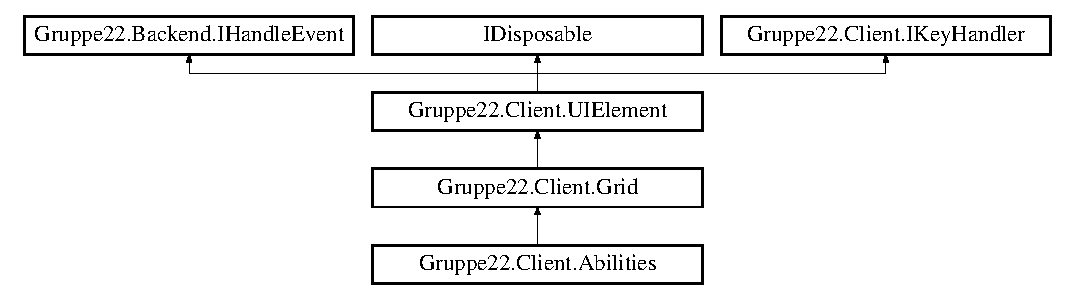
\includegraphics[height=3.589744cm]{class_gruppe22_1_1_client_1_1_abilities}
\end{center}
\end{figure}
\subsection*{Öffentliche Methoden}
\begin{DoxyCompactItemize}
\item 
override int \hyperlink{class_gruppe22_1_1_client_1_1_abilities_a736694886772621f4ef219ad8ae83aa5}{Pos2\-Tile} (int x, int y)
\item 
void \hyperlink{class_gruppe22_1_1_client_1_1_abilities_a561619cabfbdf7e279889d3bbcfedb5a}{Display\-Tool\-Tip} (int icon, int y)
\begin{DoxyCompactList}\small\item\em Append a new line of text to the status box; word wrap if necessary \end{DoxyCompactList}\item 
override bool \hyperlink{class_gruppe22_1_1_client_1_1_abilities_ae3f148ccf966b0c8157b038c0489dfa3}{On\-Mouse\-Down} (int button)
\begin{DoxyCompactList}\small\item\em Called when a mouse button changes from up to down \end{DoxyCompactList}\item 
override void \hyperlink{class_gruppe22_1_1_client_1_1_abilities_a2514f092f1e04b34a57b78866836c642}{Draw} (Game\-Time game\-Time)
\item 
\hyperlink{class_gruppe22_1_1_client_1_1_abilities_a144f390381b22116a22b929d7bd247f4}{Abilities} (\hyperlink{interface_gruppe22_1_1_backend_1_1_i_handle_event}{Backend.\-I\-Handle\-Event} parent, Sprite\-Batch sprite\-Batch, Content\-Manager content, Rectangle display\-Rect, \hyperlink{class_gruppe22_1_1_backend_1_1_actor}{Backend.\-Actor} \hyperlink{class_gruppe22_1_1_client_1_1_abilities_ac07634e3f8f741d688861a0fca304b65}{actor}=null)
\end{DoxyCompactItemize}
\subsection*{Propertys}
\begin{DoxyCompactItemize}
\item 
\hyperlink{class_gruppe22_1_1_backend_1_1_actor}{Backend.\-Actor} \hyperlink{class_gruppe22_1_1_client_1_1_abilities_ac07634e3f8f741d688861a0fca304b65}{actor}\hspace{0.3cm}{\ttfamily  \mbox{[}get, set\mbox{]}}
\end{DoxyCompactItemize}
\subsection*{Weitere Geerbte Elemente}


\subsection{Beschreibung der Konstruktoren und Destruktoren}
\hypertarget{class_gruppe22_1_1_client_1_1_abilities_a144f390381b22116a22b929d7bd247f4}{\index{Gruppe22\-::\-Client\-::\-Abilities@{Gruppe22\-::\-Client\-::\-Abilities}!Abilities@{Abilities}}
\index{Abilities@{Abilities}!Gruppe22::Client::Abilities@{Gruppe22\-::\-Client\-::\-Abilities}}
\subsubsection[{Abilities}]{\setlength{\rightskip}{0pt plus 5cm}Gruppe22.\-Client.\-Abilities.\-Abilities (
\begin{DoxyParamCaption}
\item[{{\bf Backend.\-I\-Handle\-Event}}]{parent, }
\item[{Sprite\-Batch}]{sprite\-Batch, }
\item[{Content\-Manager}]{content, }
\item[{Rectangle}]{display\-Rect, }
\item[{{\bf Backend.\-Actor}}]{actor = {\ttfamily null}}
\end{DoxyParamCaption}
)}}\label{class_gruppe22_1_1_client_1_1_abilities_a144f390381b22116a22b929d7bd247f4}


\subsection{Dokumentation der Elementfunktionen}
\hypertarget{class_gruppe22_1_1_client_1_1_abilities_a561619cabfbdf7e279889d3bbcfedb5a}{\index{Gruppe22\-::\-Client\-::\-Abilities@{Gruppe22\-::\-Client\-::\-Abilities}!Display\-Tool\-Tip@{Display\-Tool\-Tip}}
\index{Display\-Tool\-Tip@{Display\-Tool\-Tip}!Gruppe22::Client::Abilities@{Gruppe22\-::\-Client\-::\-Abilities}}
\subsubsection[{Display\-Tool\-Tip}]{\setlength{\rightskip}{0pt plus 5cm}void Gruppe22.\-Client.\-Abilities.\-Display\-Tool\-Tip (
\begin{DoxyParamCaption}
\item[{int}]{icon, }
\item[{int}]{y}
\end{DoxyParamCaption}
)}}\label{class_gruppe22_1_1_client_1_1_abilities_a561619cabfbdf7e279889d3bbcfedb5a}


Append a new line of text to the status box; word wrap if necessary 


\begin{DoxyParams}{Parameter}
{\em text} & \\
\hline
\end{DoxyParams}
\hypertarget{class_gruppe22_1_1_client_1_1_abilities_a2514f092f1e04b34a57b78866836c642}{\index{Gruppe22\-::\-Client\-::\-Abilities@{Gruppe22\-::\-Client\-::\-Abilities}!Draw@{Draw}}
\index{Draw@{Draw}!Gruppe22::Client::Abilities@{Gruppe22\-::\-Client\-::\-Abilities}}
\subsubsection[{Draw}]{\setlength{\rightskip}{0pt plus 5cm}override void Gruppe22.\-Client.\-Abilities.\-Draw (
\begin{DoxyParamCaption}
\item[{Game\-Time}]{game\-Time}
\end{DoxyParamCaption}
)\hspace{0.3cm}{\ttfamily [virtual]}}}\label{class_gruppe22_1_1_client_1_1_abilities_a2514f092f1e04b34a57b78866836c642}





\begin{DoxyParams}{Parameter}
{\em game\-Time} & \\
\hline
\end{DoxyParams}


Erneute Implementation von \hyperlink{class_gruppe22_1_1_client_1_1_u_i_element_ae68afcbd1db3540052d6b399022e56e7}{Gruppe22.\-Client.\-U\-I\-Element}.

\hypertarget{class_gruppe22_1_1_client_1_1_abilities_ae3f148ccf966b0c8157b038c0489dfa3}{\index{Gruppe22\-::\-Client\-::\-Abilities@{Gruppe22\-::\-Client\-::\-Abilities}!On\-Mouse\-Down@{On\-Mouse\-Down}}
\index{On\-Mouse\-Down@{On\-Mouse\-Down}!Gruppe22::Client::Abilities@{Gruppe22\-::\-Client\-::\-Abilities}}
\subsubsection[{On\-Mouse\-Down}]{\setlength{\rightskip}{0pt plus 5cm}override bool Gruppe22.\-Client.\-Abilities.\-On\-Mouse\-Down (
\begin{DoxyParamCaption}
\item[{int}]{button}
\end{DoxyParamCaption}
)\hspace{0.3cm}{\ttfamily [virtual]}}}\label{class_gruppe22_1_1_client_1_1_abilities_ae3f148ccf966b0c8157b038c0489dfa3}


Called when a mouse button changes from up to down 


\begin{DoxyParams}{Parameter}
{\em button} & Left \hyperlink{class_gruppe22_1_1_client_1_1_button}{Button}=1, Middle \hyperlink{class_gruppe22_1_1_client_1_1_button}{Button}=2, Right \hyperlink{class_gruppe22_1_1_client_1_1_button}{Button}=3\\
\hline
\end{DoxyParams}


Erneute Implementation von \hyperlink{class_gruppe22_1_1_client_1_1_u_i_element_a0530df2286336160b8b39c74ba380a44}{Gruppe22.\-Client.\-U\-I\-Element}.

\hypertarget{class_gruppe22_1_1_client_1_1_abilities_a736694886772621f4ef219ad8ae83aa5}{\index{Gruppe22\-::\-Client\-::\-Abilities@{Gruppe22\-::\-Client\-::\-Abilities}!Pos2\-Tile@{Pos2\-Tile}}
\index{Pos2\-Tile@{Pos2\-Tile}!Gruppe22::Client::Abilities@{Gruppe22\-::\-Client\-::\-Abilities}}
\subsubsection[{Pos2\-Tile}]{\setlength{\rightskip}{0pt plus 5cm}override int Gruppe22.\-Client.\-Abilities.\-Pos2\-Tile (
\begin{DoxyParamCaption}
\item[{int}]{x, }
\item[{int}]{y}
\end{DoxyParamCaption}
)\hspace{0.3cm}{\ttfamily [virtual]}}}\label{class_gruppe22_1_1_client_1_1_abilities_a736694886772621f4ef219ad8ae83aa5}


Erneute Implementation von \hyperlink{class_gruppe22_1_1_client_1_1_grid_a7270d988d5e751a796cfd5329cbe0967}{Gruppe22.\-Client.\-Grid}.



\subsection{Dokumentation der Propertys}
\hypertarget{class_gruppe22_1_1_client_1_1_abilities_ac07634e3f8f741d688861a0fca304b65}{\index{Gruppe22\-::\-Client\-::\-Abilities@{Gruppe22\-::\-Client\-::\-Abilities}!actor@{actor}}
\index{actor@{actor}!Gruppe22::Client::Abilities@{Gruppe22\-::\-Client\-::\-Abilities}}
\subsubsection[{actor}]{\setlength{\rightskip}{0pt plus 5cm}{\bf Backend.\-Actor} Gruppe22.\-Client.\-Abilities.\-actor\hspace{0.3cm}{\ttfamily [get]}, {\ttfamily [set]}}}\label{class_gruppe22_1_1_client_1_1_abilities_ac07634e3f8f741d688861a0fca304b65}


Die Dokumentation für diese Klasse wurde erzeugt aufgrund der Datei\-:\begin{DoxyCompactItemize}
\item 
C\-:/\-Users/beursken/\-Documents/\-Git\-Hub/gruppe22/\-Gruppe22/\-Gruppe22/\-Client/\-U\-I/\hyperlink{_abilities_8cs}{Abilities.\-cs}\end{DoxyCompactItemize}

\hypertarget{class_gruppe22_1_1_backend_1_1_ability}{\section{Gruppe22.\-Backend.\-Ability Klassenreferenz}
\label{class_gruppe22_1_1_backend_1_1_ability}\index{Gruppe22.\-Backend.\-Ability@{Gruppe22.\-Backend.\-Ability}}
}
\subsection*{Öffentliche Methoden}
\begin{DoxyCompactItemize}
\item 
void \hyperlink{class_gruppe22_1_1_backend_1_1_ability_a210e90c69a90ce45b8d1d642c9d11221}{Save} (Xml\-Writer xmlw)
\item 
void \hyperlink{class_gruppe22_1_1_backend_1_1_ability_a33373ce962eb402cdeff95b81cfae7a3}{Load} (Xml\-Reader reader)
\item 
void \hyperlink{class_gruppe22_1_1_backend_1_1_ability_a663457451c5e71c31f4048d6bd0d9514}{Generate\-Name} ()
\item 
void \hyperlink{class_gruppe22_1_1_backend_1_1_ability_ae790c08b2a22597fda3e2639db310db5}{Get\-Icon} ()
\item 
\hyperlink{class_gruppe22_1_1_backend_1_1_ability_a6af6ea05adee5c392b0cd0c83a8a74cf}{Ability} (Content\-Manager content, int \hyperlink{class_gruppe22_1_1_backend_1_1_ability_ab2f4f4b75213c665106df63903ccfe8c}{cost}=2, int \hyperlink{class_gruppe22_1_1_backend_1_1_ability_a1d46b2b7c4ef3a68baaecdd760cd1e95}{intensity}=1, int \hyperlink{class_gruppe22_1_1_backend_1_1_ability_a770e679c16231ff78f2ae8cc224c135f}{duration}=0, int \hyperlink{class_gruppe22_1_1_backend_1_1_ability_a9a046660470ca60c301cf0b5b8f74b5a}{cooldown}=5, \hyperlink{namespace_gruppe22_1_1_backend_a76255be55e4f31a7f4380aa4570b7531}{Ability\-Target} \hyperlink{class_gruppe22_1_1_backend_1_1_ability_aa77fd7c42e2d1396cd7930c6afdc4fc0}{target}=Ability\-Target.\-None, \hyperlink{namespace_gruppe22_1_1_backend_a313ed67a4abf2c938a5930323a3d6f49}{Ability\-Element} \hyperlink{class_gruppe22_1_1_backend_1_1_ability_a0025d149e70655162484fd013d6b4aa5}{element}=Ability\-Element.\-None, string \hyperlink{class_gruppe22_1_1_backend_1_1_ability_a64ef394368abef87c79e24d6383f0e41}{name}=\char`\"{}\char`\"{}, string \hyperlink{class_gruppe22_1_1_backend_1_1_ability_a98e874a3e5d992f0ae8e24e2a92dbd7e}{description}=\char`\"{}\char`\"{})
\end{DoxyCompactItemize}
\subsection*{Propertys}
\begin{DoxyCompactItemize}
\item 
int \hyperlink{class_gruppe22_1_1_backend_1_1_ability_a4c036759fa0a1c2226d590fc0dcee8b7}{improve\-Over}\hspace{0.3cm}{\ttfamily  \mbox{[}get, set\mbox{]}}
\item 
int \hyperlink{class_gruppe22_1_1_backend_1_1_ability_a770e679c16231ff78f2ae8cc224c135f}{duration}\hspace{0.3cm}{\ttfamily  \mbox{[}get, set\mbox{]}}
\item 
string \hyperlink{class_gruppe22_1_1_backend_1_1_ability_a98e874a3e5d992f0ae8e24e2a92dbd7e}{description}\hspace{0.3cm}{\ttfamily  \mbox{[}get, set\mbox{]}}
\item 
\hyperlink{class_gruppe22_1_1_backend_1_1_image_data}{Image\-Data} \hyperlink{class_gruppe22_1_1_backend_1_1_ability_a524886d89b0f96454632e6b788f320df}{icon}\hspace{0.3cm}{\ttfamily  \mbox{[}get, set\mbox{]}}
\item 
string \hyperlink{class_gruppe22_1_1_backend_1_1_ability_a64ef394368abef87c79e24d6383f0e41}{name}\hspace{0.3cm}{\ttfamily  \mbox{[}get, set\mbox{]}}
\item 
int \hyperlink{class_gruppe22_1_1_backend_1_1_ability_af26f712be0a6b8d55cc71a3dc936fa1e}{current\-Cool}\hspace{0.3cm}{\ttfamily  \mbox{[}get, set\mbox{]}}
\item 
int \hyperlink{class_gruppe22_1_1_backend_1_1_ability_ab2f4f4b75213c665106df63903ccfe8c}{cost}\hspace{0.3cm}{\ttfamily  \mbox{[}get, set\mbox{]}}
\item 
int \hyperlink{class_gruppe22_1_1_backend_1_1_ability_a1d46b2b7c4ef3a68baaecdd760cd1e95}{intensity}\hspace{0.3cm}{\ttfamily  \mbox{[}get, set\mbox{]}}
\item 
int \hyperlink{class_gruppe22_1_1_backend_1_1_ability_a9a046660470ca60c301cf0b5b8f74b5a}{cooldown}\hspace{0.3cm}{\ttfamily  \mbox{[}get, set\mbox{]}}
\item 
\hyperlink{namespace_gruppe22_1_1_backend_a76255be55e4f31a7f4380aa4570b7531}{Ability\-Target} \hyperlink{class_gruppe22_1_1_backend_1_1_ability_aa77fd7c42e2d1396cd7930c6afdc4fc0}{target}\hspace{0.3cm}{\ttfamily  \mbox{[}get, set\mbox{]}}
\item 
\hyperlink{namespace_gruppe22_1_1_backend_a313ed67a4abf2c938a5930323a3d6f49}{Ability\-Element} \hyperlink{class_gruppe22_1_1_backend_1_1_ability_a0025d149e70655162484fd013d6b4aa5}{element}\hspace{0.3cm}{\ttfamily  \mbox{[}get, set\mbox{]}}
\end{DoxyCompactItemize}


\subsection{Beschreibung der Konstruktoren und Destruktoren}
\hypertarget{class_gruppe22_1_1_backend_1_1_ability_a6af6ea05adee5c392b0cd0c83a8a74cf}{\index{Gruppe22\-::\-Backend\-::\-Ability@{Gruppe22\-::\-Backend\-::\-Ability}!Ability@{Ability}}
\index{Ability@{Ability}!Gruppe22::Backend::Ability@{Gruppe22\-::\-Backend\-::\-Ability}}
\subsubsection[{Ability}]{\setlength{\rightskip}{0pt plus 5cm}Gruppe22.\-Backend.\-Ability.\-Ability (
\begin{DoxyParamCaption}
\item[{Content\-Manager}]{content, }
\item[{int}]{cost = {\ttfamily 2}, }
\item[{int}]{intensity = {\ttfamily 1}, }
\item[{int}]{duration = {\ttfamily 0}, }
\item[{int}]{cooldown = {\ttfamily 5}, }
\item[{{\bf Ability\-Target}}]{target = {\ttfamily AbilityTarget.None}, }
\item[{{\bf Ability\-Element}}]{element = {\ttfamily AbilityElement.None}, }
\item[{string}]{name = {\ttfamily \char`\"{}\char`\"{}}, }
\item[{string}]{description = {\ttfamily \char`\"{}\char`\"{}}}
\end{DoxyParamCaption}
)}}\label{class_gruppe22_1_1_backend_1_1_ability_a6af6ea05adee5c392b0cd0c83a8a74cf}


\subsection{Dokumentation der Elementfunktionen}
\hypertarget{class_gruppe22_1_1_backend_1_1_ability_a663457451c5e71c31f4048d6bd0d9514}{\index{Gruppe22\-::\-Backend\-::\-Ability@{Gruppe22\-::\-Backend\-::\-Ability}!Generate\-Name@{Generate\-Name}}
\index{Generate\-Name@{Generate\-Name}!Gruppe22::Backend::Ability@{Gruppe22\-::\-Backend\-::\-Ability}}
\subsubsection[{Generate\-Name}]{\setlength{\rightskip}{0pt plus 5cm}void Gruppe22.\-Backend.\-Ability.\-Generate\-Name (
\begin{DoxyParamCaption}
{}
\end{DoxyParamCaption}
)}}\label{class_gruppe22_1_1_backend_1_1_ability_a663457451c5e71c31f4048d6bd0d9514}
\hypertarget{class_gruppe22_1_1_backend_1_1_ability_ae790c08b2a22597fda3e2639db310db5}{\index{Gruppe22\-::\-Backend\-::\-Ability@{Gruppe22\-::\-Backend\-::\-Ability}!Get\-Icon@{Get\-Icon}}
\index{Get\-Icon@{Get\-Icon}!Gruppe22::Backend::Ability@{Gruppe22\-::\-Backend\-::\-Ability}}
\subsubsection[{Get\-Icon}]{\setlength{\rightskip}{0pt plus 5cm}void Gruppe22.\-Backend.\-Ability.\-Get\-Icon (
\begin{DoxyParamCaption}
{}
\end{DoxyParamCaption}
)}}\label{class_gruppe22_1_1_backend_1_1_ability_ae790c08b2a22597fda3e2639db310db5}
\hypertarget{class_gruppe22_1_1_backend_1_1_ability_a33373ce962eb402cdeff95b81cfae7a3}{\index{Gruppe22\-::\-Backend\-::\-Ability@{Gruppe22\-::\-Backend\-::\-Ability}!Load@{Load}}
\index{Load@{Load}!Gruppe22::Backend::Ability@{Gruppe22\-::\-Backend\-::\-Ability}}
\subsubsection[{Load}]{\setlength{\rightskip}{0pt plus 5cm}void Gruppe22.\-Backend.\-Ability.\-Load (
\begin{DoxyParamCaption}
\item[{Xml\-Reader}]{reader}
\end{DoxyParamCaption}
)}}\label{class_gruppe22_1_1_backend_1_1_ability_a33373ce962eb402cdeff95b81cfae7a3}





\begin{DoxyParams}{Parameter}
{\em reader} & \\
\hline
\end{DoxyParams}
\hypertarget{class_gruppe22_1_1_backend_1_1_ability_a210e90c69a90ce45b8d1d642c9d11221}{\index{Gruppe22\-::\-Backend\-::\-Ability@{Gruppe22\-::\-Backend\-::\-Ability}!Save@{Save}}
\index{Save@{Save}!Gruppe22::Backend::Ability@{Gruppe22\-::\-Backend\-::\-Ability}}
\subsubsection[{Save}]{\setlength{\rightskip}{0pt plus 5cm}void Gruppe22.\-Backend.\-Ability.\-Save (
\begin{DoxyParamCaption}
\item[{Xml\-Writer}]{xmlw}
\end{DoxyParamCaption}
)}}\label{class_gruppe22_1_1_backend_1_1_ability_a210e90c69a90ce45b8d1d642c9d11221}


\subsection{Dokumentation der Propertys}
\hypertarget{class_gruppe22_1_1_backend_1_1_ability_a9a046660470ca60c301cf0b5b8f74b5a}{\index{Gruppe22\-::\-Backend\-::\-Ability@{Gruppe22\-::\-Backend\-::\-Ability}!cooldown@{cooldown}}
\index{cooldown@{cooldown}!Gruppe22::Backend::Ability@{Gruppe22\-::\-Backend\-::\-Ability}}
\subsubsection[{cooldown}]{\setlength{\rightskip}{0pt plus 5cm}int Gruppe22.\-Backend.\-Ability.\-cooldown\hspace{0.3cm}{\ttfamily [get]}, {\ttfamily [set]}}}\label{class_gruppe22_1_1_backend_1_1_ability_a9a046660470ca60c301cf0b5b8f74b5a}
\hypertarget{class_gruppe22_1_1_backend_1_1_ability_ab2f4f4b75213c665106df63903ccfe8c}{\index{Gruppe22\-::\-Backend\-::\-Ability@{Gruppe22\-::\-Backend\-::\-Ability}!cost@{cost}}
\index{cost@{cost}!Gruppe22::Backend::Ability@{Gruppe22\-::\-Backend\-::\-Ability}}
\subsubsection[{cost}]{\setlength{\rightskip}{0pt plus 5cm}int Gruppe22.\-Backend.\-Ability.\-cost\hspace{0.3cm}{\ttfamily [get]}, {\ttfamily [set]}}}\label{class_gruppe22_1_1_backend_1_1_ability_ab2f4f4b75213c665106df63903ccfe8c}
\hypertarget{class_gruppe22_1_1_backend_1_1_ability_af26f712be0a6b8d55cc71a3dc936fa1e}{\index{Gruppe22\-::\-Backend\-::\-Ability@{Gruppe22\-::\-Backend\-::\-Ability}!current\-Cool@{current\-Cool}}
\index{current\-Cool@{current\-Cool}!Gruppe22::Backend::Ability@{Gruppe22\-::\-Backend\-::\-Ability}}
\subsubsection[{current\-Cool}]{\setlength{\rightskip}{0pt plus 5cm}int Gruppe22.\-Backend.\-Ability.\-current\-Cool\hspace{0.3cm}{\ttfamily [get]}, {\ttfamily [set]}}}\label{class_gruppe22_1_1_backend_1_1_ability_af26f712be0a6b8d55cc71a3dc936fa1e}
\hypertarget{class_gruppe22_1_1_backend_1_1_ability_a98e874a3e5d992f0ae8e24e2a92dbd7e}{\index{Gruppe22\-::\-Backend\-::\-Ability@{Gruppe22\-::\-Backend\-::\-Ability}!description@{description}}
\index{description@{description}!Gruppe22::Backend::Ability@{Gruppe22\-::\-Backend\-::\-Ability}}
\subsubsection[{description}]{\setlength{\rightskip}{0pt plus 5cm}string Gruppe22.\-Backend.\-Ability.\-description\hspace{0.3cm}{\ttfamily [get]}, {\ttfamily [set]}}}\label{class_gruppe22_1_1_backend_1_1_ability_a98e874a3e5d992f0ae8e24e2a92dbd7e}
\hypertarget{class_gruppe22_1_1_backend_1_1_ability_a770e679c16231ff78f2ae8cc224c135f}{\index{Gruppe22\-::\-Backend\-::\-Ability@{Gruppe22\-::\-Backend\-::\-Ability}!duration@{duration}}
\index{duration@{duration}!Gruppe22::Backend::Ability@{Gruppe22\-::\-Backend\-::\-Ability}}
\subsubsection[{duration}]{\setlength{\rightskip}{0pt plus 5cm}int Gruppe22.\-Backend.\-Ability.\-duration\hspace{0.3cm}{\ttfamily [get]}, {\ttfamily [set]}}}\label{class_gruppe22_1_1_backend_1_1_ability_a770e679c16231ff78f2ae8cc224c135f}
\hypertarget{class_gruppe22_1_1_backend_1_1_ability_a0025d149e70655162484fd013d6b4aa5}{\index{Gruppe22\-::\-Backend\-::\-Ability@{Gruppe22\-::\-Backend\-::\-Ability}!element@{element}}
\index{element@{element}!Gruppe22::Backend::Ability@{Gruppe22\-::\-Backend\-::\-Ability}}
\subsubsection[{element}]{\setlength{\rightskip}{0pt plus 5cm}{\bf Ability\-Element} Gruppe22.\-Backend.\-Ability.\-element\hspace{0.3cm}{\ttfamily [get]}, {\ttfamily [set]}}}\label{class_gruppe22_1_1_backend_1_1_ability_a0025d149e70655162484fd013d6b4aa5}
\hypertarget{class_gruppe22_1_1_backend_1_1_ability_a524886d89b0f96454632e6b788f320df}{\index{Gruppe22\-::\-Backend\-::\-Ability@{Gruppe22\-::\-Backend\-::\-Ability}!icon@{icon}}
\index{icon@{icon}!Gruppe22::Backend::Ability@{Gruppe22\-::\-Backend\-::\-Ability}}
\subsubsection[{icon}]{\setlength{\rightskip}{0pt plus 5cm}{\bf Image\-Data} Gruppe22.\-Backend.\-Ability.\-icon\hspace{0.3cm}{\ttfamily [get]}, {\ttfamily [set]}}}\label{class_gruppe22_1_1_backend_1_1_ability_a524886d89b0f96454632e6b788f320df}
\hypertarget{class_gruppe22_1_1_backend_1_1_ability_a4c036759fa0a1c2226d590fc0dcee8b7}{\index{Gruppe22\-::\-Backend\-::\-Ability@{Gruppe22\-::\-Backend\-::\-Ability}!improve\-Over@{improve\-Over}}
\index{improve\-Over@{improve\-Over}!Gruppe22::Backend::Ability@{Gruppe22\-::\-Backend\-::\-Ability}}
\subsubsection[{improve\-Over}]{\setlength{\rightskip}{0pt plus 5cm}int Gruppe22.\-Backend.\-Ability.\-improve\-Over\hspace{0.3cm}{\ttfamily [get]}, {\ttfamily [set]}}}\label{class_gruppe22_1_1_backend_1_1_ability_a4c036759fa0a1c2226d590fc0dcee8b7}
\hypertarget{class_gruppe22_1_1_backend_1_1_ability_a1d46b2b7c4ef3a68baaecdd760cd1e95}{\index{Gruppe22\-::\-Backend\-::\-Ability@{Gruppe22\-::\-Backend\-::\-Ability}!intensity@{intensity}}
\index{intensity@{intensity}!Gruppe22::Backend::Ability@{Gruppe22\-::\-Backend\-::\-Ability}}
\subsubsection[{intensity}]{\setlength{\rightskip}{0pt plus 5cm}int Gruppe22.\-Backend.\-Ability.\-intensity\hspace{0.3cm}{\ttfamily [get]}, {\ttfamily [set]}}}\label{class_gruppe22_1_1_backend_1_1_ability_a1d46b2b7c4ef3a68baaecdd760cd1e95}
\hypertarget{class_gruppe22_1_1_backend_1_1_ability_a64ef394368abef87c79e24d6383f0e41}{\index{Gruppe22\-::\-Backend\-::\-Ability@{Gruppe22\-::\-Backend\-::\-Ability}!name@{name}}
\index{name@{name}!Gruppe22::Backend::Ability@{Gruppe22\-::\-Backend\-::\-Ability}}
\subsubsection[{name}]{\setlength{\rightskip}{0pt plus 5cm}string Gruppe22.\-Backend.\-Ability.\-name\hspace{0.3cm}{\ttfamily [get]}, {\ttfamily [set]}}}\label{class_gruppe22_1_1_backend_1_1_ability_a64ef394368abef87c79e24d6383f0e41}
\hypertarget{class_gruppe22_1_1_backend_1_1_ability_aa77fd7c42e2d1396cd7930c6afdc4fc0}{\index{Gruppe22\-::\-Backend\-::\-Ability@{Gruppe22\-::\-Backend\-::\-Ability}!target@{target}}
\index{target@{target}!Gruppe22::Backend::Ability@{Gruppe22\-::\-Backend\-::\-Ability}}
\subsubsection[{target}]{\setlength{\rightskip}{0pt plus 5cm}{\bf Ability\-Target} Gruppe22.\-Backend.\-Ability.\-target\hspace{0.3cm}{\ttfamily [get]}, {\ttfamily [set]}}}\label{class_gruppe22_1_1_backend_1_1_ability_aa77fd7c42e2d1396cd7930c6afdc4fc0}


Die Dokumentation für diese Klasse wurde erzeugt aufgrund der Datei\-:\begin{DoxyCompactItemize}
\item 
C\-:/\-Users/beursken/\-Documents/\-Git\-Hub/gruppe22/\-Gruppe22/\-Gruppe22/\-Backend/\-Items/\hyperlink{_ability_8cs}{Ability.\-cs}\end{DoxyCompactItemize}

\hypertarget{class_gruppe22_1_1_client_1_1_ability_choice}{\section{Gruppe22.\-Client.\-Ability\-Choice Klassenreferenz}
\label{class_gruppe22_1_1_client_1_1_ability_choice}\index{Gruppe22.\-Client.\-Ability\-Choice@{Gruppe22.\-Client.\-Ability\-Choice}}
}
Klassendiagramm für Gruppe22.\-Client.\-Ability\-Choice\-:\begin{figure}[H]
\begin{center}
\leavevmode
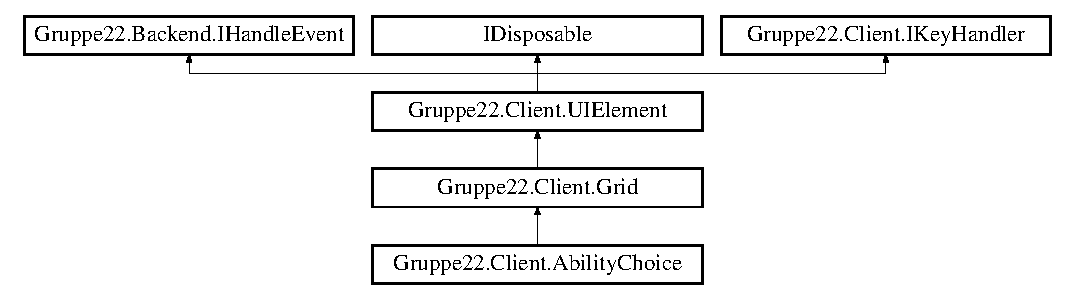
\includegraphics[height=3.589744cm]{class_gruppe22_1_1_client_1_1_ability_choice}
\end{center}
\end{figure}
\subsection*{Öffentliche Methoden}
\begin{DoxyCompactItemize}
\item 
override bool \hyperlink{class_gruppe22_1_1_client_1_1_ability_choice_a15b4f981409cdc4b6f8c94a50e0df81f}{On\-Mouse\-Down} (int button)
\begin{DoxyCompactList}\small\item\em Called when a mouse button changes from up to down \end{DoxyCompactList}\item 
override int \hyperlink{class_gruppe22_1_1_client_1_1_ability_choice_a8a27d3ed23f7d873aff9a73e70775c87}{Pos2\-Tile} (int x, int y)
\item 
void \hyperlink{class_gruppe22_1_1_client_1_1_ability_choice_aad5248a5ad8c9e2b6126b12570e48006}{Generate\-Ability} (int id)
\item 
override void \hyperlink{class_gruppe22_1_1_client_1_1_ability_choice_ac4fc4ffdc4771811c6252d1da748127a}{Draw} (Game\-Time game\-Time)
\item 
void \hyperlink{class_gruppe22_1_1_client_1_1_ability_choice_a21bda333dd5c3f3b8b7583b38ba9bd38}{Display\-Tool\-Tip} (int icon)
\begin{DoxyCompactList}\small\item\em Append a new line of text to the status box; word wrap if necessary \end{DoxyCompactList}\item 
\hyperlink{class_gruppe22_1_1_client_1_1_ability_choice_a105763bd56b618db7f05091f013d0890}{Ability\-Choice} (\hyperlink{interface_gruppe22_1_1_backend_1_1_i_handle_event}{Backend.\-I\-Handle\-Event} parent, Sprite\-Batch sprite\-Batch, Content\-Manager content, Rectangle display\-Rect, \hyperlink{class_gruppe22_1_1_backend_1_1_actor}{Backend.\-Actor} \hyperlink{class_gruppe22_1_1_client_1_1_ability_choice_a6ba233119143416fd07771ab05b8b7c9}{actor}=null)
\end{DoxyCompactItemize}
\subsection*{Propertys}
\begin{DoxyCompactItemize}
\item 
\hyperlink{class_gruppe22_1_1_backend_1_1_actor}{Backend.\-Actor} \hyperlink{class_gruppe22_1_1_client_1_1_ability_choice_a6ba233119143416fd07771ab05b8b7c9}{actor}\hspace{0.3cm}{\ttfamily  \mbox{[}get, set\mbox{]}}
\end{DoxyCompactItemize}
\subsection*{Weitere Geerbte Elemente}


\subsection{Beschreibung der Konstruktoren und Destruktoren}
\hypertarget{class_gruppe22_1_1_client_1_1_ability_choice_a105763bd56b618db7f05091f013d0890}{\index{Gruppe22\-::\-Client\-::\-Ability\-Choice@{Gruppe22\-::\-Client\-::\-Ability\-Choice}!Ability\-Choice@{Ability\-Choice}}
\index{Ability\-Choice@{Ability\-Choice}!Gruppe22::Client::AbilityChoice@{Gruppe22\-::\-Client\-::\-Ability\-Choice}}
\subsubsection[{Ability\-Choice}]{\setlength{\rightskip}{0pt plus 5cm}Gruppe22.\-Client.\-Ability\-Choice.\-Ability\-Choice (
\begin{DoxyParamCaption}
\item[{{\bf Backend.\-I\-Handle\-Event}}]{parent, }
\item[{Sprite\-Batch}]{sprite\-Batch, }
\item[{Content\-Manager}]{content, }
\item[{Rectangle}]{display\-Rect, }
\item[{{\bf Backend.\-Actor}}]{actor = {\ttfamily null}}
\end{DoxyParamCaption}
)}}\label{class_gruppe22_1_1_client_1_1_ability_choice_a105763bd56b618db7f05091f013d0890}


\subsection{Dokumentation der Elementfunktionen}
\hypertarget{class_gruppe22_1_1_client_1_1_ability_choice_a21bda333dd5c3f3b8b7583b38ba9bd38}{\index{Gruppe22\-::\-Client\-::\-Ability\-Choice@{Gruppe22\-::\-Client\-::\-Ability\-Choice}!Display\-Tool\-Tip@{Display\-Tool\-Tip}}
\index{Display\-Tool\-Tip@{Display\-Tool\-Tip}!Gruppe22::Client::AbilityChoice@{Gruppe22\-::\-Client\-::\-Ability\-Choice}}
\subsubsection[{Display\-Tool\-Tip}]{\setlength{\rightskip}{0pt plus 5cm}void Gruppe22.\-Client.\-Ability\-Choice.\-Display\-Tool\-Tip (
\begin{DoxyParamCaption}
\item[{int}]{icon}
\end{DoxyParamCaption}
)}}\label{class_gruppe22_1_1_client_1_1_ability_choice_a21bda333dd5c3f3b8b7583b38ba9bd38}


Append a new line of text to the status box; word wrap if necessary 


\begin{DoxyParams}{Parameter}
{\em text} & \\
\hline
\end{DoxyParams}
\hypertarget{class_gruppe22_1_1_client_1_1_ability_choice_ac4fc4ffdc4771811c6252d1da748127a}{\index{Gruppe22\-::\-Client\-::\-Ability\-Choice@{Gruppe22\-::\-Client\-::\-Ability\-Choice}!Draw@{Draw}}
\index{Draw@{Draw}!Gruppe22::Client::AbilityChoice@{Gruppe22\-::\-Client\-::\-Ability\-Choice}}
\subsubsection[{Draw}]{\setlength{\rightskip}{0pt plus 5cm}override void Gruppe22.\-Client.\-Ability\-Choice.\-Draw (
\begin{DoxyParamCaption}
\item[{Game\-Time}]{game\-Time}
\end{DoxyParamCaption}
)\hspace{0.3cm}{\ttfamily [virtual]}}}\label{class_gruppe22_1_1_client_1_1_ability_choice_ac4fc4ffdc4771811c6252d1da748127a}





\begin{DoxyParams}{Parameter}
{\em game\-Time} & \\
\hline
\end{DoxyParams}


Erneute Implementation von \hyperlink{class_gruppe22_1_1_client_1_1_u_i_element_ae68afcbd1db3540052d6b399022e56e7}{Gruppe22.\-Client.\-U\-I\-Element}.

\hypertarget{class_gruppe22_1_1_client_1_1_ability_choice_aad5248a5ad8c9e2b6126b12570e48006}{\index{Gruppe22\-::\-Client\-::\-Ability\-Choice@{Gruppe22\-::\-Client\-::\-Ability\-Choice}!Generate\-Ability@{Generate\-Ability}}
\index{Generate\-Ability@{Generate\-Ability}!Gruppe22::Client::AbilityChoice@{Gruppe22\-::\-Client\-::\-Ability\-Choice}}
\subsubsection[{Generate\-Ability}]{\setlength{\rightskip}{0pt plus 5cm}void Gruppe22.\-Client.\-Ability\-Choice.\-Generate\-Ability (
\begin{DoxyParamCaption}
\item[{int}]{id}
\end{DoxyParamCaption}
)}}\label{class_gruppe22_1_1_client_1_1_ability_choice_aad5248a5ad8c9e2b6126b12570e48006}
\hypertarget{class_gruppe22_1_1_client_1_1_ability_choice_a15b4f981409cdc4b6f8c94a50e0df81f}{\index{Gruppe22\-::\-Client\-::\-Ability\-Choice@{Gruppe22\-::\-Client\-::\-Ability\-Choice}!On\-Mouse\-Down@{On\-Mouse\-Down}}
\index{On\-Mouse\-Down@{On\-Mouse\-Down}!Gruppe22::Client::AbilityChoice@{Gruppe22\-::\-Client\-::\-Ability\-Choice}}
\subsubsection[{On\-Mouse\-Down}]{\setlength{\rightskip}{0pt plus 5cm}override bool Gruppe22.\-Client.\-Ability\-Choice.\-On\-Mouse\-Down (
\begin{DoxyParamCaption}
\item[{int}]{button}
\end{DoxyParamCaption}
)\hspace{0.3cm}{\ttfamily [virtual]}}}\label{class_gruppe22_1_1_client_1_1_ability_choice_a15b4f981409cdc4b6f8c94a50e0df81f}


Called when a mouse button changes from up to down 


\begin{DoxyParams}{Parameter}
{\em button} & Left \hyperlink{class_gruppe22_1_1_client_1_1_button}{Button}=1, Middle \hyperlink{class_gruppe22_1_1_client_1_1_button}{Button}=2, Right \hyperlink{class_gruppe22_1_1_client_1_1_button}{Button}=3\\
\hline
\end{DoxyParams}


Erneute Implementation von \hyperlink{class_gruppe22_1_1_client_1_1_u_i_element_a0530df2286336160b8b39c74ba380a44}{Gruppe22.\-Client.\-U\-I\-Element}.

\hypertarget{class_gruppe22_1_1_client_1_1_ability_choice_a8a27d3ed23f7d873aff9a73e70775c87}{\index{Gruppe22\-::\-Client\-::\-Ability\-Choice@{Gruppe22\-::\-Client\-::\-Ability\-Choice}!Pos2\-Tile@{Pos2\-Tile}}
\index{Pos2\-Tile@{Pos2\-Tile}!Gruppe22::Client::AbilityChoice@{Gruppe22\-::\-Client\-::\-Ability\-Choice}}
\subsubsection[{Pos2\-Tile}]{\setlength{\rightskip}{0pt plus 5cm}override int Gruppe22.\-Client.\-Ability\-Choice.\-Pos2\-Tile (
\begin{DoxyParamCaption}
\item[{int}]{x, }
\item[{int}]{y}
\end{DoxyParamCaption}
)\hspace{0.3cm}{\ttfamily [virtual]}}}\label{class_gruppe22_1_1_client_1_1_ability_choice_a8a27d3ed23f7d873aff9a73e70775c87}


Erneute Implementation von \hyperlink{class_gruppe22_1_1_client_1_1_grid_a7270d988d5e751a796cfd5329cbe0967}{Gruppe22.\-Client.\-Grid}.



\subsection{Dokumentation der Propertys}
\hypertarget{class_gruppe22_1_1_client_1_1_ability_choice_a6ba233119143416fd07771ab05b8b7c9}{\index{Gruppe22\-::\-Client\-::\-Ability\-Choice@{Gruppe22\-::\-Client\-::\-Ability\-Choice}!actor@{actor}}
\index{actor@{actor}!Gruppe22::Client::AbilityChoice@{Gruppe22\-::\-Client\-::\-Ability\-Choice}}
\subsubsection[{actor}]{\setlength{\rightskip}{0pt plus 5cm}{\bf Backend.\-Actor} Gruppe22.\-Client.\-Ability\-Choice.\-actor\hspace{0.3cm}{\ttfamily [get]}, {\ttfamily [set]}}}\label{class_gruppe22_1_1_client_1_1_ability_choice_a6ba233119143416fd07771ab05b8b7c9}


Die Dokumentation für diese Klasse wurde erzeugt aufgrund der Datei\-:\begin{DoxyCompactItemize}
\item 
C\-:/\-Users/beursken/\-Documents/\-Git\-Hub/gruppe22/\-Gruppe22/\-Gruppe22/\-Client/\-U\-I/\hyperlink{_ability_choice_8cs}{Ability\-Choice.\-cs}\end{DoxyCompactItemize}

\hypertarget{class_gruppe22_1_1_backend_1_1_actor}{\section{Gruppe22.\-Backend.\-Actor Klassenreferenz}
\label{class_gruppe22_1_1_backend_1_1_actor}\index{Gruppe22.\-Backend.\-Actor@{Gruppe22.\-Backend.\-Actor}}
}
Klassendiagramm für Gruppe22.\-Backend.\-Actor\-:\begin{figure}[H]
\begin{center}
\leavevmode
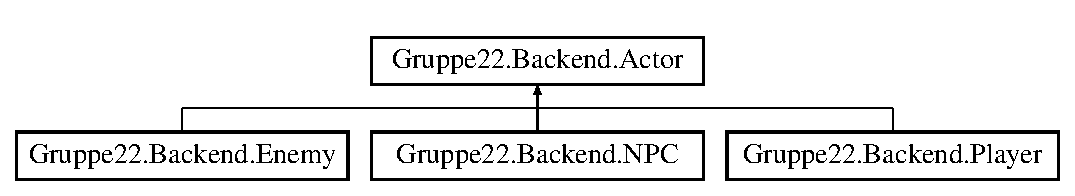
\includegraphics[height=2.000000cm]{class_gruppe22_1_1_backend_1_1_actor}
\end{center}
\end{figure}
\subsection*{Öffentliche Methoden}
\begin{DoxyCompactItemize}
\item 
\hyperlink{class_gruppe22_1_1_backend_1_1_item}{Item} \hyperlink{class_gruppe22_1_1_backend_1_1_actor_a5df320c3507d76483563a06002bcdc0a}{Items} (int i)
\item 
void \hyperlink{class_gruppe22_1_1_backend_1_1_actor_a01868add985a927294354d6b9a1d7004}{Regen} ()
\item 
void \hyperlink{class_gruppe22_1_1_backend_1_1_actor_aaa131c6048e5f34d460ff68888f92172}{Level\-Up} ()
\item 
void \hyperlink{class_gruppe22_1_1_backend_1_1_actor_a46b6acd21e36621b69811af94b0c85a1}{Add\-Protection} (int amount)
\item 
void \hyperlink{class_gruppe22_1_1_backend_1_1_actor_aebee25827f86035b50d452fbbc8d3f1f}{Add\-Health} (int amount)
\item 
void \hyperlink{class_gruppe22_1_1_backend_1_1_actor_a00c58df999ffc13c17fb9b2a33e0434e}{Add\-Strength} (int amount)
\begin{DoxyCompactList}\small\item\em T\-O\-D\-O\-: Versstehe ich nicht was die genau tut \end{DoxyCompactList}\item 
void \hyperlink{class_gruppe22_1_1_backend_1_1_actor_ad6372297e223c485ca0d885091edd7f4}{Save} (Xml\-Writer writer)
\begin{DoxyCompactList}\small\item\em Savemethode. Speichert die N\-P\-C-\/\-Daten im writer. \end{DoxyCompactList}\item 
bool \hyperlink{class_gruppe22_1_1_backend_1_1_actor_a48b6120de07360ef561a4d40fcbe17b6}{Has\-Key} (int \hyperlink{class_gruppe22_1_1_backend_1_1_actor_aef8ca8637a54602399de1b2d08670c9e}{level})
\begin{DoxyCompactList}\small\item\em Methode gibt an ob der Spieler den S\-Chlüssel für Level level schon aufgehoben hat. \end{DoxyCompactList}\item 
void \hyperlink{class_gruppe22_1_1_backend_1_1_actor_aec58c47e2019cfc9eeede1b0ac7ee788}{copy\-From} (\hyperlink{class_gruppe22_1_1_backend_1_1_actor}{Actor} a)
\begin{DoxyCompactList}\small\item\em Klont alle Actor-\/\-Eigenschaften von a. \end{DoxyCompactList}\item 
void \hyperlink{class_gruppe22_1_1_backend_1_1_actor_abab30b54b556a93fb68044299f57a13f}{Load} (Xml\-Reader reader)
\begin{DoxyCompactList}\small\item\em a method to read an actor from a (room-\/)file and set his values \end{DoxyCompactList}\item 
override string \hyperlink{class_gruppe22_1_1_backend_1_1_actor_a8aee9e4883cce82a031244e62a725077}{To\-String} ()
\item 
void \hyperlink{class_gruppe22_1_1_backend_1_1_actor_a91da621907674e6fd7403143a609e858}{Generate\-Name} ()
\begin{DoxyCompactList}\small\item\em Methode to generate random names for actors uses \hyperlink{class_gruppe22_1_1_backend_1_1_actor_a91da621907674e6fd7403143a609e858}{Generate\-Name()} for files if possible \end{DoxyCompactList}\item 
string \hyperlink{class_gruppe22_1_1_backend_1_1_actor_ab355b820e866805831fde9aa92064549}{Generate\-Name} (string filename)
\begin{DoxyCompactList}\small\item\em Method to generate a random name from a given file \end{DoxyCompactList}\item 
\hyperlink{class_gruppe22_1_1_backend_1_1_actor_ab11640b7f9bced587bf5a568197194c4}{Actor} (Content\-Manager content, \hyperlink{namespace_gruppe22_1_1_backend_a56d8f7bd1b5ba29d421c27a959523af3}{Actor\-Type} \hyperlink{class_gruppe22_1_1_backend_1_1_actor_a58c387d62c241bbafdb677144f121afb}{actor\-Type}, int \hyperlink{class_gruppe22_1_1_backend_1_1_actor_a46f3a7d62de83a6bf3c44cd52f38af9b}{health}, int \hyperlink{class_gruppe22_1_1_backend_1_1_actor_ab400f0b82f96d2334891d7cd428f5d08}{armor}, int \hyperlink{class_gruppe22_1_1_backend_1_1_actor_a461e2480a59de23517c3b375dede10fb}{damage}, int \hyperlink{class_gruppe22_1_1_backend_1_1_actor_aac0f2f9a2f0b314f98ba19d0b38a7a97}{max\-Health}=-\/1, string \hyperlink{class_gruppe22_1_1_backend_1_1_actor_a28129eaf9d70d9bfc33a29544ba74edf}{name}=\char`\"{}\char`\"{}, Random rnd=null, string \hyperlink{class_gruppe22_1_1_backend_1_1_actor_a95b868d16d310a817634fe8498ad9667}{animation\-File}=\char`\"{}\char`\"{}, int \hyperlink{class_gruppe22_1_1_backend_1_1_actor_aef8ca8637a54602399de1b2d08670c9e}{level}=-\/1)
\begin{DoxyCompactList}\small\item\em Konstruktor. \end{DoxyCompactList}\end{DoxyCompactItemize}
\subsection*{Öffentliche Attribute}
\begin{DoxyCompactItemize}
\item 
List$<$ int $>$ \hyperlink{class_gruppe22_1_1_backend_1_1_actor_a82d6e523cc6a9f60302a8208d0636f37}{\-\_\-quicklist} = null
\end{DoxyCompactItemize}
\subsection*{Geschützte Attribute}
\begin{DoxyCompactItemize}
\item 
Random \hyperlink{class_gruppe22_1_1_backend_1_1_actor_a4080b008472d54be9578f0e5fafde8fd}{\-\_\-random}
\item 
int \hyperlink{class_gruppe22_1_1_backend_1_1_actor_a97f8959538541fb8fb2a1f1a51ed37af}{\-\_\-new\-Items} = 0
\item 
\hyperlink{class_gruppe22_1_1_backend_1_1_actor_tile}{Actor\-Tile} \hyperlink{class_gruppe22_1_1_backend_1_1_actor_aa18bcd4363b23f8a4eef003ee26a830f}{\-\_\-tile}
\item 
\hyperlink{namespace_gruppe22_1_1_backend_a56d8f7bd1b5ba29d421c27a959523af3}{Actor\-Type} \hyperlink{class_gruppe22_1_1_backend_1_1_actor_a00cc8cd745cd8b3e25e7114cbd4a2073}{\-\_\-actor\-Type}
\item 
int \hyperlink{class_gruppe22_1_1_backend_1_1_actor_a5ce8fbbf6e837f50fd73dde0b8727441}{\-\_\-id} = 0
\item 
string \hyperlink{class_gruppe22_1_1_backend_1_1_actor_abe357b249386e48968f23fe0440e6828}{\-\_\-name} = \char`\"{}\char`\"{}
\item 
List$<$ \hyperlink{class_gruppe22_1_1_backend_1_1_item}{Item} $>$ \hyperlink{class_gruppe22_1_1_backend_1_1_actor_ad20845ea7fd5ae4ffaefa5b5c3ce485a}{\-\_\-inventory} = null
\item 
int \hyperlink{class_gruppe22_1_1_backend_1_1_actor_a9ed1576fe639441364e86d1e38f124ea}{\-\_\-mana} = 50
\item 
int \hyperlink{class_gruppe22_1_1_backend_1_1_actor_a06c3f8a3312eb5e80e5b8e01de17ca18}{\-\_\-evade} = 0
\item 
int \hyperlink{class_gruppe22_1_1_backend_1_1_actor_a9948c30b99e0f88c1b68515cfdbdcdfe}{\-\_\-block} = 0
\item 
int \hyperlink{class_gruppe22_1_1_backend_1_1_actor_ae39864b12f85addfa4efab1544cf8c1c}{\-\_\-penetrate} = 0
\item 
int \hyperlink{class_gruppe22_1_1_backend_1_1_actor_a07a1b23b0018abc02409b3ef06dfc2d6}{\-\_\-health\-Reg} = 0
\item 
int \hyperlink{class_gruppe22_1_1_backend_1_1_actor_ae6d971300eb5b899ffa0445a44a5c991}{\-\_\-steal\-Health} = 0
\item 
int \hyperlink{class_gruppe22_1_1_backend_1_1_actor_aaf873521206419ec8e47290fd0fdf067}{\-\_\-steal\-Mana} = 0
\item 
int \hyperlink{class_gruppe22_1_1_backend_1_1_actor_a6ae70043ed745c8b68e25ccbc8998b7d}{\-\_\-fire\-Damage} = 0
\item 
int \hyperlink{class_gruppe22_1_1_backend_1_1_actor_a98151c4328eda7afbdf4e82b7836ca2e}{\-\_\-ice\-Damage} = 0
\item 
int \hyperlink{class_gruppe22_1_1_backend_1_1_actor_ac2a5b48aa9544dc5551112808bd4731c}{\-\_\-fire\-Defense} = 0
\item 
int \hyperlink{class_gruppe22_1_1_backend_1_1_actor_ae8e34de866ae050de9fb6fbcf3078dfa}{\-\_\-ice\-Defense} = 0
\item 
int \hyperlink{class_gruppe22_1_1_backend_1_1_actor_ad6d527ba7fea76c45716ba1d659db8a8}{\-\_\-destroy\-Weapon} = 0
\item 
int \hyperlink{class_gruppe22_1_1_backend_1_1_actor_aa4f9a1ba2e6bbae3f132dbef3e1312cc}{\-\_\-destroy\-Armor} = 0
\item 
int \hyperlink{class_gruppe22_1_1_backend_1_1_actor_a306b56f7a4b82420f91b6ba9fc8560d0}{\-\_\-max\-Mana} = 100
\item 
int \hyperlink{class_gruppe22_1_1_backend_1_1_actor_a7f6c14f4dacf65a00af7d3fb56d4c24a}{\-\_\-mana\-Reg} = 0
\item 
int \hyperlink{class_gruppe22_1_1_backend_1_1_actor_ad39870dc0fbc9a37764183ccee6de616}{\-\_\-gold} = 0
\item 
bool \hyperlink{class_gruppe22_1_1_backend_1_1_actor_a34cce380159de650fc7742befd9f44e0}{\-\_\-locked} = false
\item 
int \hyperlink{class_gruppe22_1_1_backend_1_1_actor_ace31c72a0fd9bb941df7112647dff86d}{\-\_\-level} = 0
\item 
int \hyperlink{class_gruppe22_1_1_backend_1_1_actor_a76c1dfdeff49bbdc1dce9927171eff5f}{\-\_\-damage} = 0
\item 
bool \hyperlink{class_gruppe22_1_1_backend_1_1_actor_a0b42acc54218d8d0b6f671088bbfc671}{\-\_\-aggro} = true
\item 
bool \hyperlink{class_gruppe22_1_1_backend_1_1_actor_a177e17548afa61e77b15c341e1cc4e14}{\-\_\-ranged} = false
\item 
bool \hyperlink{class_gruppe22_1_1_backend_1_1_actor_abfb9be7927de3f5c3c221eef43404005}{\-\_\-crazy} = false
\item 
bool \hyperlink{class_gruppe22_1_1_backend_1_1_actor_ae9ad82d44eefcad479c8dff093ef3c8b}{\-\_\-friendly} = false
\item 
int \hyperlink{class_gruppe22_1_1_backend_1_1_actor_a8f5daef5dca70eb646ee7d6c20efec57}{\-\_\-resist} = 0
\item 
int \hyperlink{class_gruppe22_1_1_backend_1_1_actor_aa16348ec720da67371dbe08b3e7c0e3b}{\-\_\-exp} = 0
\item 
int \hyperlink{class_gruppe22_1_1_backend_1_1_actor_a92de167ad37109b84bf56d0d1bea17d5}{\-\_\-exp\-Needed} = 0
\item 
int \hyperlink{class_gruppe22_1_1_backend_1_1_actor_a661db1997d023af860bfe43043a057b9}{\-\_\-maxhealth} = 100
\item 
int \hyperlink{class_gruppe22_1_1_backend_1_1_actor_abd832633228ad53ca314bf41888f453c}{\-\_\-health} = 50
\item 
int \hyperlink{class_gruppe22_1_1_backend_1_1_actor_aaabaf99935dcfcf861ae81380629300f}{\-\_\-armor} = 40
\item 
int \hyperlink{class_gruppe22_1_1_backend_1_1_actor_ac1939716818aaa3d7dd72d58e3271e15}{\-\_\-ability\-Points} = 0
\item 
int \hyperlink{class_gruppe22_1_1_backend_1_1_actor_afa1bd09529e5040b6a32aae11fa1735f}{\-\_\-skills} = 0
\item 
Content\-Manager \hyperlink{class_gruppe22_1_1_backend_1_1_actor_af412b616dc48c16a2633155c44462852}{\-\_\-content}
\item 
int \hyperlink{class_gruppe22_1_1_backend_1_1_actor_a346e9109439573ab536ab6ee819b4959}{\-\_\-view\-Range} = 4
\item 
string \hyperlink{class_gruppe22_1_1_backend_1_1_actor_a4808e957128607a9828b5c664bce2dc8}{\-\_\-animation\-File} = \char`\"{}.\textbackslash{}\textbackslash{}content\textbackslash{}\textbackslash{}player.\-xml\char`\"{}
\item 
int \hyperlink{class_gruppe22_1_1_backend_1_1_actor_a1e9b1c145b4b5a88a3fe1ba706ffed23}{\-\_\-stunned} = 0
\item 
int \hyperlink{class_gruppe22_1_1_backend_1_1_actor_ae84ade4a1e62477765d6819d029f2355}{\-\_\-charmed} = 0
\item 
int \hyperlink{class_gruppe22_1_1_backend_1_1_actor_a0cb71e4de44e6c9c114b3a43f7d196f8}{\-\_\-scared} = 0
\item 
List$<$ \hyperlink{class_gruppe22_1_1_backend_1_1_ability}{Ability} $>$ \hyperlink{class_gruppe22_1_1_backend_1_1_actor_ab14f7cd68b782e54e1a32295a83ea874}{\-\_\-abilities} = null
\end{DoxyCompactItemize}
\subsection*{Propertys}
\begin{DoxyCompactItemize}
\item 
int \hyperlink{class_gruppe22_1_1_backend_1_1_actor_a1f51fc8c39ecccdcbd0172426aa7e92d}{new\-Items}\hspace{0.3cm}{\ttfamily  \mbox{[}get, set\mbox{]}}
\item 
int \hyperlink{class_gruppe22_1_1_backend_1_1_actor_a7dc16682680a355fb8ba501de5c97f86}{view\-Range}\hspace{0.3cm}{\ttfamily  \mbox{[}get, set\mbox{]}}
\item 
int \hyperlink{class_gruppe22_1_1_backend_1_1_actor_a246e1e15bbdca1fd85f6cd1c36c5f659}{scared}\hspace{0.3cm}{\ttfamily  \mbox{[}get, set\mbox{]}}
\item 
int \hyperlink{class_gruppe22_1_1_backend_1_1_actor_aa06c0673dcd07f618d9c49a27e1c6864}{stunned}\hspace{0.3cm}{\ttfamily  \mbox{[}get, set\mbox{]}}
\item 
int \hyperlink{class_gruppe22_1_1_backend_1_1_actor_a1be7d3366a3f72a9f81d069b32cfffbb}{charmed}\hspace{0.3cm}{\ttfamily  \mbox{[}get, set\mbox{]}}
\item 
List$<$ int $>$ \hyperlink{class_gruppe22_1_1_backend_1_1_actor_aab796f965d79d55e09fbd4f4e35459b6}{quick\-List}\hspace{0.3cm}{\ttfamily  \mbox{[}get, set\mbox{]}}
\item 
bool \hyperlink{class_gruppe22_1_1_backend_1_1_actor_a0ef711c60615b8e01de20fe6e3f993c0}{friendly}\hspace{0.3cm}{\ttfamily  \mbox{[}get, set\mbox{]}}
\item 
bool \hyperlink{class_gruppe22_1_1_backend_1_1_actor_a90a081611e6ccddf379b5caf3ba9fcd0}{aggro}\hspace{0.3cm}{\ttfamily  \mbox{[}get, set\mbox{]}}
\item 
bool \hyperlink{class_gruppe22_1_1_backend_1_1_actor_aed1184696fffba422c8c795b127d6bf3}{crazy}\hspace{0.3cm}{\ttfamily  \mbox{[}get, set\mbox{]}}
\item 
bool \hyperlink{class_gruppe22_1_1_backend_1_1_actor_a878185cb8cd096ceac0bd20f5aa17b2c}{ranged}\hspace{0.3cm}{\ttfamily  \mbox{[}get, set\mbox{]}}
\item 
bool \hyperlink{class_gruppe22_1_1_backend_1_1_actor_a83141441f0192f33ec936375138c5c0a}{locked}\hspace{0.3cm}{\ttfamily  \mbox{[}get, set\mbox{]}}
\item 
string \hyperlink{class_gruppe22_1_1_backend_1_1_actor_a95b868d16d310a817634fe8498ad9667}{animation\-File}\hspace{0.3cm}{\ttfamily  \mbox{[}get, set\mbox{]}}
\item 
\hyperlink{class_gruppe22_1_1_backend_1_1_actor_tile}{Actor\-Tile} \hyperlink{class_gruppe22_1_1_backend_1_1_actor_aa7ad76c503eeb79619e23151a18b1ffe}{tile}\hspace{0.3cm}{\ttfamily  \mbox{[}get, set\mbox{]}}
\item 
List$<$ \hyperlink{class_gruppe22_1_1_backend_1_1_item}{Item} $>$ \hyperlink{class_gruppe22_1_1_backend_1_1_actor_a050ee718b5ffd0148b000f67e1f8881e}{inventory}\hspace{0.3cm}{\ttfamily  \mbox{[}get\mbox{]}}
\item 
List$<$ \hyperlink{class_gruppe22_1_1_backend_1_1_ability}{Ability} $>$ \hyperlink{class_gruppe22_1_1_backend_1_1_actor_a001807714d4d692e47488c56d6300725}{abilities}\hspace{0.3cm}{\ttfamily  \mbox{[}get\mbox{]}}
\item 
int \hyperlink{class_gruppe22_1_1_backend_1_1_actor_a048f1d94ca8de4b039838201b1f0c562}{mana}\hspace{0.3cm}{\ttfamily  \mbox{[}get, set\mbox{]}}
\item 
int \hyperlink{class_gruppe22_1_1_backend_1_1_actor_aba93e7913cf8bbdef58d48c6f64cc69e}{exp\-Needed}\hspace{0.3cm}{\ttfamily  \mbox{[}get, set\mbox{]}}
\item 
int \hyperlink{class_gruppe22_1_1_backend_1_1_actor_a7aa937ebf6ab96040f2a5c396dc39bf3}{max\-Mana}\hspace{0.3cm}{\ttfamily  \mbox{[}get, set\mbox{]}}
\item 
int \hyperlink{class_gruppe22_1_1_backend_1_1_actor_a30731ee8851baca8b03d185131d660d8}{mana\-Reg}\hspace{0.3cm}{\ttfamily  \mbox{[}get, set\mbox{]}}
\item 
int \hyperlink{class_gruppe22_1_1_backend_1_1_actor_ae48dbaa79fc8f5754c25917238358cd9}{gold}\hspace{0.3cm}{\ttfamily  \mbox{[}get, set\mbox{]}}
\item 
\hyperlink{namespace_gruppe22_1_1_backend_a56d8f7bd1b5ba29d421c27a959523af3}{Actor\-Type} \hyperlink{class_gruppe22_1_1_backend_1_1_actor_a58c387d62c241bbafdb677144f121afb}{actor\-Type}\hspace{0.3cm}{\ttfamily  \mbox{[}get\mbox{]}}
\item 
int \hyperlink{class_gruppe22_1_1_backend_1_1_actor_a46f3a7d62de83a6bf3c44cd52f38af9b}{health}\hspace{0.3cm}{\ttfamily  \mbox{[}get, set\mbox{]}}
\item 
int \hyperlink{class_gruppe22_1_1_backend_1_1_actor_aac0f2f9a2f0b314f98ba19d0b38a7a97}{max\-Health}\hspace{0.3cm}{\ttfamily  \mbox{[}get, set\mbox{]}}
\item 
int \hyperlink{class_gruppe22_1_1_backend_1_1_actor_ab400f0b82f96d2334891d7cd428f5d08}{armor}\hspace{0.3cm}{\ttfamily  \mbox{[}get, set\mbox{]}}
\item 
int \hyperlink{class_gruppe22_1_1_backend_1_1_actor_a461e2480a59de23517c3b375dede10fb}{damage}\hspace{0.3cm}{\ttfamily  \mbox{[}get, set\mbox{]}}
\item 
string \hyperlink{class_gruppe22_1_1_backend_1_1_actor_a28129eaf9d70d9bfc33a29544ba74edf}{name}\hspace{0.3cm}{\ttfamily  \mbox{[}get, set\mbox{]}}
\item 
int \hyperlink{class_gruppe22_1_1_backend_1_1_actor_aef8ca8637a54602399de1b2d08670c9e}{level}\hspace{0.3cm}{\ttfamily  \mbox{[}get\mbox{]}}
\item 
int \hyperlink{class_gruppe22_1_1_backend_1_1_actor_a6f6054da9e996138615a79d3e7cf605e}{exp}\hspace{0.3cm}{\ttfamily  \mbox{[}get, set\mbox{]}}
\item 
bool \hyperlink{class_gruppe22_1_1_backend_1_1_actor_aa6209f07df8dc4e292dc7223f2286531}{is\-Dead}\hspace{0.3cm}{\ttfamily  \mbox{[}get\mbox{]}}
\item 
int \hyperlink{class_gruppe22_1_1_backend_1_1_actor_adcde4f63fe800423d0b9847b4446541a}{id}\hspace{0.3cm}{\ttfamily  \mbox{[}get, set\mbox{]}}
\item 
int \hyperlink{class_gruppe22_1_1_backend_1_1_actor_ac9d50048cd67c8c33c220787c9e1b2bd}{evade}\hspace{0.3cm}{\ttfamily  \mbox{[}get, set\mbox{]}}
\item 
int \hyperlink{class_gruppe22_1_1_backend_1_1_actor_a7afca219b61d6b43769ebb9c3a7a909c}{block}\hspace{0.3cm}{\ttfamily  \mbox{[}get, set\mbox{]}}
\item 
int \hyperlink{class_gruppe22_1_1_backend_1_1_actor_a2f685f79b4afc83118844d8daf5a9383}{penetrate}\hspace{0.3cm}{\ttfamily  \mbox{[}get, set\mbox{]}}
\item 
int \hyperlink{class_gruppe22_1_1_backend_1_1_actor_aa1846abb97dd0514823f23d3f21ef26e}{health\-Reg}\hspace{0.3cm}{\ttfamily  \mbox{[}get, set\mbox{]}}
\item 
int \hyperlink{class_gruppe22_1_1_backend_1_1_actor_a292546a8315a784e5619295685de5733}{steal\-Health}\hspace{0.3cm}{\ttfamily  \mbox{[}get, set\mbox{]}}
\item 
int \hyperlink{class_gruppe22_1_1_backend_1_1_actor_a557d850a0079cfeef19664f5543ea05f}{steal\-Mana}\hspace{0.3cm}{\ttfamily  \mbox{[}get, set\mbox{]}}
\item 
int \hyperlink{class_gruppe22_1_1_backend_1_1_actor_a4d4696df6455a267542b45fae67d9263}{fire\-Damage}\hspace{0.3cm}{\ttfamily  \mbox{[}get, set\mbox{]}}
\item 
int \hyperlink{class_gruppe22_1_1_backend_1_1_actor_acf33a1adc5b6e8a31f60b47d02e65753}{ice\-Damage}\hspace{0.3cm}{\ttfamily  \mbox{[}get, set\mbox{]}}
\item 
int \hyperlink{class_gruppe22_1_1_backend_1_1_actor_a9faae4ca664fad2c2cae3590c487a2a2}{fire\-Defense}\hspace{0.3cm}{\ttfamily  \mbox{[}get, set\mbox{]}}
\item 
int \hyperlink{class_gruppe22_1_1_backend_1_1_actor_a4b228c6a5523929eaaba0d19e2fe8736}{ice\-Defense}\hspace{0.3cm}{\ttfamily  \mbox{[}get, set\mbox{]}}
\item 
int \hyperlink{class_gruppe22_1_1_backend_1_1_actor_a2b219112882a726377db085058faa362}{destroy\-Weapon}\hspace{0.3cm}{\ttfamily  \mbox{[}get, set\mbox{]}}
\item 
int \hyperlink{class_gruppe22_1_1_backend_1_1_actor_ac66d30c3eca8daa01c9db6563eeb3461}{destroy\-Armor}\hspace{0.3cm}{\ttfamily  \mbox{[}get, set\mbox{]}}
\item 
int \hyperlink{class_gruppe22_1_1_backend_1_1_actor_a923139471b3d24df0ab9ac42de1381e1}{resist}\hspace{0.3cm}{\ttfamily  \mbox{[}get, set\mbox{]}}
\item 
int \hyperlink{class_gruppe22_1_1_backend_1_1_actor_a0edcdc56082f4d806c41500f4eba7330}{maxhealth}\hspace{0.3cm}{\ttfamily  \mbox{[}get, set\mbox{]}}
\item 
int \hyperlink{class_gruppe22_1_1_backend_1_1_actor_a2f7eb00667b49ff7c525ddfc8bd50963}{ability\-Points}\hspace{0.3cm}{\ttfamily  \mbox{[}get, set\mbox{]}}
\item 
int \hyperlink{class_gruppe22_1_1_backend_1_1_actor_afd0c138a8626821ef4a749a457eb1f06}{skills}\hspace{0.3cm}{\ttfamily  \mbox{[}get, set\mbox{]}}
\end{DoxyCompactItemize}


\subsection{Beschreibung der Konstruktoren und Destruktoren}
\hypertarget{class_gruppe22_1_1_backend_1_1_actor_ab11640b7f9bced587bf5a568197194c4}{\index{Gruppe22\-::\-Backend\-::\-Actor@{Gruppe22\-::\-Backend\-::\-Actor}!Actor@{Actor}}
\index{Actor@{Actor}!Gruppe22::Backend::Actor@{Gruppe22\-::\-Backend\-::\-Actor}}
\subsubsection[{Actor}]{\setlength{\rightskip}{0pt plus 5cm}Gruppe22.\-Backend.\-Actor.\-Actor (
\begin{DoxyParamCaption}
\item[{Content\-Manager}]{content, }
\item[{{\bf Actor\-Type}}]{actor\-Type, }
\item[{int}]{health, }
\item[{int}]{armor, }
\item[{int}]{damage, }
\item[{int}]{max\-Health = {\ttfamily -\/1}, }
\item[{string}]{name = {\ttfamily \char`\"{}\char`\"{}}, }
\item[{Random}]{rnd = {\ttfamily null}, }
\item[{string}]{animation\-File = {\ttfamily \char`\"{}\char`\"{}}, }
\item[{int}]{level = {\ttfamily -\/1}}
\end{DoxyParamCaption}
)}}\label{class_gruppe22_1_1_backend_1_1_actor_ab11640b7f9bced587bf5a568197194c4}


Konstruktor. 


\begin{DoxyParams}{Parameter}
{\em content} & \\
\hline
{\em actor\-Type} & \hyperlink{class_gruppe22_1_1_backend_1_1_player}{Player}, \hyperlink{class_gruppe22_1_1_backend_1_1_n_p_c}{N\-P\-C} or \hyperlink{class_gruppe22_1_1_backend_1_1_enemy}{Enemy}\\
\hline
{\em health} & default 15+random(30) or 5+random(maxhealth-\/5) if maxhealth is passed\\
\hline
{\em armor} & default random(10)\\
\hline
{\em damage} & default 12+random(10)\\
\hline
{\em max\-Health} & default = health\\
\hline
{\em name} & uses \hyperlink{class_gruppe22_1_1_backend_1_1_actor_a91da621907674e6fd7403143a609e858}{Generate\-Name()} by default\\
\hline
{\em rnd} & a random used to generate the actors starting values\\
\hline
{\em animation\-File} & the file used to display the actor\\
\hline
{\em level} & the default starting level is 1\\
\hline
\end{DoxyParams}


\subsection{Dokumentation der Elementfunktionen}
\hypertarget{class_gruppe22_1_1_backend_1_1_actor_aebee25827f86035b50d452fbbc8d3f1f}{\index{Gruppe22\-::\-Backend\-::\-Actor@{Gruppe22\-::\-Backend\-::\-Actor}!Add\-Health@{Add\-Health}}
\index{Add\-Health@{Add\-Health}!Gruppe22::Backend::Actor@{Gruppe22\-::\-Backend\-::\-Actor}}
\subsubsection[{Add\-Health}]{\setlength{\rightskip}{0pt plus 5cm}void Gruppe22.\-Backend.\-Actor.\-Add\-Health (
\begin{DoxyParamCaption}
\item[{int}]{amount}
\end{DoxyParamCaption}
)}}\label{class_gruppe22_1_1_backend_1_1_actor_aebee25827f86035b50d452fbbc8d3f1f}





\begin{DoxyParams}{Parameter}
{\em amount} & \\
\hline
\end{DoxyParams}
\hypertarget{class_gruppe22_1_1_backend_1_1_actor_a46b6acd21e36621b69811af94b0c85a1}{\index{Gruppe22\-::\-Backend\-::\-Actor@{Gruppe22\-::\-Backend\-::\-Actor}!Add\-Protection@{Add\-Protection}}
\index{Add\-Protection@{Add\-Protection}!Gruppe22::Backend::Actor@{Gruppe22\-::\-Backend\-::\-Actor}}
\subsubsection[{Add\-Protection}]{\setlength{\rightskip}{0pt plus 5cm}void Gruppe22.\-Backend.\-Actor.\-Add\-Protection (
\begin{DoxyParamCaption}
\item[{int}]{amount}
\end{DoxyParamCaption}
)}}\label{class_gruppe22_1_1_backend_1_1_actor_a46b6acd21e36621b69811af94b0c85a1}





\begin{DoxyParams}{Parameter}
{\em amount} & \\
\hline
\end{DoxyParams}
\hypertarget{class_gruppe22_1_1_backend_1_1_actor_a00c58df999ffc13c17fb9b2a33e0434e}{\index{Gruppe22\-::\-Backend\-::\-Actor@{Gruppe22\-::\-Backend\-::\-Actor}!Add\-Strength@{Add\-Strength}}
\index{Add\-Strength@{Add\-Strength}!Gruppe22::Backend::Actor@{Gruppe22\-::\-Backend\-::\-Actor}}
\subsubsection[{Add\-Strength}]{\setlength{\rightskip}{0pt plus 5cm}void Gruppe22.\-Backend.\-Actor.\-Add\-Strength (
\begin{DoxyParamCaption}
\item[{int}]{amount}
\end{DoxyParamCaption}
)}}\label{class_gruppe22_1_1_backend_1_1_actor_a00c58df999ffc13c17fb9b2a33e0434e}


T\-O\-D\-O\-: Versstehe ich nicht was die genau tut 


\begin{DoxyParams}{Parameter}
{\em amount} & T\-O\-D\-O\-: vo allem was ist das?\\
\hline
\end{DoxyParams}
\hypertarget{class_gruppe22_1_1_backend_1_1_actor_aec58c47e2019cfc9eeede1b0ac7ee788}{\index{Gruppe22\-::\-Backend\-::\-Actor@{Gruppe22\-::\-Backend\-::\-Actor}!copy\-From@{copy\-From}}
\index{copy\-From@{copy\-From}!Gruppe22::Backend::Actor@{Gruppe22\-::\-Backend\-::\-Actor}}
\subsubsection[{copy\-From}]{\setlength{\rightskip}{0pt plus 5cm}void Gruppe22.\-Backend.\-Actor.\-copy\-From (
\begin{DoxyParamCaption}
\item[{{\bf Actor}}]{a}
\end{DoxyParamCaption}
)}}\label{class_gruppe22_1_1_backend_1_1_actor_aec58c47e2019cfc9eeede1b0ac7ee788}


Klont alle Actor-\/\-Eigenschaften von a. 


\begin{DoxyParams}{Parameter}
{\em a} & Das Actor-\/\-Objekt von dem die Eigenschaften übernommen werden sollen.\\
\hline
\end{DoxyParams}
\hypertarget{class_gruppe22_1_1_backend_1_1_actor_a91da621907674e6fd7403143a609e858}{\index{Gruppe22\-::\-Backend\-::\-Actor@{Gruppe22\-::\-Backend\-::\-Actor}!Generate\-Name@{Generate\-Name}}
\index{Generate\-Name@{Generate\-Name}!Gruppe22::Backend::Actor@{Gruppe22\-::\-Backend\-::\-Actor}}
\subsubsection[{Generate\-Name}]{\setlength{\rightskip}{0pt plus 5cm}void Gruppe22.\-Backend.\-Actor.\-Generate\-Name (
\begin{DoxyParamCaption}
{}
\end{DoxyParamCaption}
)}}\label{class_gruppe22_1_1_backend_1_1_actor_a91da621907674e6fd7403143a609e858}


Methode to generate random names for actors uses \hyperlink{class_gruppe22_1_1_backend_1_1_actor_a91da621907674e6fd7403143a609e858}{Generate\-Name()} for files if possible 

\hypertarget{class_gruppe22_1_1_backend_1_1_actor_ab355b820e866805831fde9aa92064549}{\index{Gruppe22\-::\-Backend\-::\-Actor@{Gruppe22\-::\-Backend\-::\-Actor}!Generate\-Name@{Generate\-Name}}
\index{Generate\-Name@{Generate\-Name}!Gruppe22::Backend::Actor@{Gruppe22\-::\-Backend\-::\-Actor}}
\subsubsection[{Generate\-Name}]{\setlength{\rightskip}{0pt plus 5cm}string Gruppe22.\-Backend.\-Actor.\-Generate\-Name (
\begin{DoxyParamCaption}
\item[{string}]{filename}
\end{DoxyParamCaption}
)}}\label{class_gruppe22_1_1_backend_1_1_actor_ab355b820e866805831fde9aa92064549}


Method to generate a random name from a given file 


\begin{DoxyParams}{Parameter}
{\em filename} & a file with one name in each line\\
\hline
\end{DoxyParams}
\begin{DoxyReturn}{Rückgabe}
the chosen name
\end{DoxyReturn}
\hypertarget{class_gruppe22_1_1_backend_1_1_actor_a48b6120de07360ef561a4d40fcbe17b6}{\index{Gruppe22\-::\-Backend\-::\-Actor@{Gruppe22\-::\-Backend\-::\-Actor}!Has\-Key@{Has\-Key}}
\index{Has\-Key@{Has\-Key}!Gruppe22::Backend::Actor@{Gruppe22\-::\-Backend\-::\-Actor}}
\subsubsection[{Has\-Key}]{\setlength{\rightskip}{0pt plus 5cm}bool Gruppe22.\-Backend.\-Actor.\-Has\-Key (
\begin{DoxyParamCaption}
\item[{int}]{level}
\end{DoxyParamCaption}
)}}\label{class_gruppe22_1_1_backend_1_1_actor_a48b6120de07360ef561a4d40fcbe17b6}


Methode gibt an ob der Spieler den S\-Chlüssel für Level level schon aufgehoben hat. 


\begin{DoxyParams}{Parameter}
{\em level} & Level.\\
\hline
\end{DoxyParams}
\begin{DoxyReturn}{Rückgabe}
True wenn Schlüssel aufgenommen wurde, sonst false.
\end{DoxyReturn}
\hypertarget{class_gruppe22_1_1_backend_1_1_actor_a5df320c3507d76483563a06002bcdc0a}{\index{Gruppe22\-::\-Backend\-::\-Actor@{Gruppe22\-::\-Backend\-::\-Actor}!Items@{Items}}
\index{Items@{Items}!Gruppe22::Backend::Actor@{Gruppe22\-::\-Backend\-::\-Actor}}
\subsubsection[{Items}]{\setlength{\rightskip}{0pt plus 5cm}{\bf Item} Gruppe22.\-Backend.\-Actor.\-Items (
\begin{DoxyParamCaption}
\item[{int}]{i}
\end{DoxyParamCaption}
)}}\label{class_gruppe22_1_1_backend_1_1_actor_a5df320c3507d76483563a06002bcdc0a}
\hypertarget{class_gruppe22_1_1_backend_1_1_actor_aaa131c6048e5f34d460ff68888f92172}{\index{Gruppe22\-::\-Backend\-::\-Actor@{Gruppe22\-::\-Backend\-::\-Actor}!Level\-Up@{Level\-Up}}
\index{Level\-Up@{Level\-Up}!Gruppe22::Backend::Actor@{Gruppe22\-::\-Backend\-::\-Actor}}
\subsubsection[{Level\-Up}]{\setlength{\rightskip}{0pt plus 5cm}void Gruppe22.\-Backend.\-Actor.\-Level\-Up (
\begin{DoxyParamCaption}
{}
\end{DoxyParamCaption}
)}}\label{class_gruppe22_1_1_backend_1_1_actor_aaa131c6048e5f34d460ff68888f92172}
\hypertarget{class_gruppe22_1_1_backend_1_1_actor_abab30b54b556a93fb68044299f57a13f}{\index{Gruppe22\-::\-Backend\-::\-Actor@{Gruppe22\-::\-Backend\-::\-Actor}!Load@{Load}}
\index{Load@{Load}!Gruppe22::Backend::Actor@{Gruppe22\-::\-Backend\-::\-Actor}}
\subsubsection[{Load}]{\setlength{\rightskip}{0pt plus 5cm}void Gruppe22.\-Backend.\-Actor.\-Load (
\begin{DoxyParamCaption}
\item[{Xml\-Reader}]{reader}
\end{DoxyParamCaption}
)}}\label{class_gruppe22_1_1_backend_1_1_actor_abab30b54b556a93fb68044299f57a13f}


a method to read an actor from a (room-\/)file and set his values 


\begin{DoxyParams}{Parameter}
{\em reader} & the Xml\-Reader which should be used\\
\hline
\end{DoxyParams}
\hypertarget{class_gruppe22_1_1_backend_1_1_actor_a01868add985a927294354d6b9a1d7004}{\index{Gruppe22\-::\-Backend\-::\-Actor@{Gruppe22\-::\-Backend\-::\-Actor}!Regen@{Regen}}
\index{Regen@{Regen}!Gruppe22::Backend::Actor@{Gruppe22\-::\-Backend\-::\-Actor}}
\subsubsection[{Regen}]{\setlength{\rightskip}{0pt plus 5cm}void Gruppe22.\-Backend.\-Actor.\-Regen (
\begin{DoxyParamCaption}
{}
\end{DoxyParamCaption}
)}}\label{class_gruppe22_1_1_backend_1_1_actor_a01868add985a927294354d6b9a1d7004}
\hypertarget{class_gruppe22_1_1_backend_1_1_actor_ad6372297e223c485ca0d885091edd7f4}{\index{Gruppe22\-::\-Backend\-::\-Actor@{Gruppe22\-::\-Backend\-::\-Actor}!Save@{Save}}
\index{Save@{Save}!Gruppe22::Backend::Actor@{Gruppe22\-::\-Backend\-::\-Actor}}
\subsubsection[{Save}]{\setlength{\rightskip}{0pt plus 5cm}void Gruppe22.\-Backend.\-Actor.\-Save (
\begin{DoxyParamCaption}
\item[{Xml\-Writer}]{writer}
\end{DoxyParamCaption}
)}}\label{class_gruppe22_1_1_backend_1_1_actor_ad6372297e223c485ca0d885091edd7f4}


Savemethode. Speichert die N\-P\-C-\/\-Daten im writer. 


\begin{DoxyParams}{Parameter}
{\em writer} & Writer für die Kartendatei.\\
\hline
\end{DoxyParams}
\hypertarget{class_gruppe22_1_1_backend_1_1_actor_a8aee9e4883cce82a031244e62a725077}{\index{Gruppe22\-::\-Backend\-::\-Actor@{Gruppe22\-::\-Backend\-::\-Actor}!To\-String@{To\-String}}
\index{To\-String@{To\-String}!Gruppe22::Backend::Actor@{Gruppe22\-::\-Backend\-::\-Actor}}
\subsubsection[{To\-String}]{\setlength{\rightskip}{0pt plus 5cm}override string Gruppe22.\-Backend.\-Actor.\-To\-String (
\begin{DoxyParamCaption}
{}
\end{DoxyParamCaption}
)}}\label{class_gruppe22_1_1_backend_1_1_actor_a8aee9e4883cce82a031244e62a725077}


\subsection{Dokumentation der Datenelemente}
\hypertarget{class_gruppe22_1_1_backend_1_1_actor_ab14f7cd68b782e54e1a32295a83ea874}{\index{Gruppe22\-::\-Backend\-::\-Actor@{Gruppe22\-::\-Backend\-::\-Actor}!\-\_\-abilities@{\-\_\-abilities}}
\index{\-\_\-abilities@{\-\_\-abilities}!Gruppe22::Backend::Actor@{Gruppe22\-::\-Backend\-::\-Actor}}
\subsubsection[{\-\_\-abilities}]{\setlength{\rightskip}{0pt plus 5cm}List$<${\bf Ability}$>$ Gruppe22.\-Backend.\-Actor.\-\_\-abilities = null\hspace{0.3cm}{\ttfamily [protected]}}}\label{class_gruppe22_1_1_backend_1_1_actor_ab14f7cd68b782e54e1a32295a83ea874}
\hypertarget{class_gruppe22_1_1_backend_1_1_actor_ac1939716818aaa3d7dd72d58e3271e15}{\index{Gruppe22\-::\-Backend\-::\-Actor@{Gruppe22\-::\-Backend\-::\-Actor}!\-\_\-ability\-Points@{\-\_\-ability\-Points}}
\index{\-\_\-ability\-Points@{\-\_\-ability\-Points}!Gruppe22::Backend::Actor@{Gruppe22\-::\-Backend\-::\-Actor}}
\subsubsection[{\-\_\-ability\-Points}]{\setlength{\rightskip}{0pt plus 5cm}int Gruppe22.\-Backend.\-Actor.\-\_\-ability\-Points = 0\hspace{0.3cm}{\ttfamily [protected]}}}\label{class_gruppe22_1_1_backend_1_1_actor_ac1939716818aaa3d7dd72d58e3271e15}
\hypertarget{class_gruppe22_1_1_backend_1_1_actor_a00cc8cd745cd8b3e25e7114cbd4a2073}{\index{Gruppe22\-::\-Backend\-::\-Actor@{Gruppe22\-::\-Backend\-::\-Actor}!\-\_\-actor\-Type@{\-\_\-actor\-Type}}
\index{\-\_\-actor\-Type@{\-\_\-actor\-Type}!Gruppe22::Backend::Actor@{Gruppe22\-::\-Backend\-::\-Actor}}
\subsubsection[{\-\_\-actor\-Type}]{\setlength{\rightskip}{0pt plus 5cm}{\bf Actor\-Type} Gruppe22.\-Backend.\-Actor.\-\_\-actor\-Type\hspace{0.3cm}{\ttfamily [protected]}}}\label{class_gruppe22_1_1_backend_1_1_actor_a00cc8cd745cd8b3e25e7114cbd4a2073}
\hypertarget{class_gruppe22_1_1_backend_1_1_actor_a0b42acc54218d8d0b6f671088bbfc671}{\index{Gruppe22\-::\-Backend\-::\-Actor@{Gruppe22\-::\-Backend\-::\-Actor}!\-\_\-aggro@{\-\_\-aggro}}
\index{\-\_\-aggro@{\-\_\-aggro}!Gruppe22::Backend::Actor@{Gruppe22\-::\-Backend\-::\-Actor}}
\subsubsection[{\-\_\-aggro}]{\setlength{\rightskip}{0pt plus 5cm}bool Gruppe22.\-Backend.\-Actor.\-\_\-aggro = true\hspace{0.3cm}{\ttfamily [protected]}}}\label{class_gruppe22_1_1_backend_1_1_actor_a0b42acc54218d8d0b6f671088bbfc671}
\hypertarget{class_gruppe22_1_1_backend_1_1_actor_a4808e957128607a9828b5c664bce2dc8}{\index{Gruppe22\-::\-Backend\-::\-Actor@{Gruppe22\-::\-Backend\-::\-Actor}!\-\_\-animation\-File@{\-\_\-animation\-File}}
\index{\-\_\-animation\-File@{\-\_\-animation\-File}!Gruppe22::Backend::Actor@{Gruppe22\-::\-Backend\-::\-Actor}}
\subsubsection[{\-\_\-animation\-File}]{\setlength{\rightskip}{0pt plus 5cm}string Gruppe22.\-Backend.\-Actor.\-\_\-animation\-File = \char`\"{}.\textbackslash{}\textbackslash{}content\textbackslash{}\textbackslash{}player.\-xml\char`\"{}\hspace{0.3cm}{\ttfamily [protected]}}}\label{class_gruppe22_1_1_backend_1_1_actor_a4808e957128607a9828b5c664bce2dc8}
\hypertarget{class_gruppe22_1_1_backend_1_1_actor_aaabaf99935dcfcf861ae81380629300f}{\index{Gruppe22\-::\-Backend\-::\-Actor@{Gruppe22\-::\-Backend\-::\-Actor}!\-\_\-armor@{\-\_\-armor}}
\index{\-\_\-armor@{\-\_\-armor}!Gruppe22::Backend::Actor@{Gruppe22\-::\-Backend\-::\-Actor}}
\subsubsection[{\-\_\-armor}]{\setlength{\rightskip}{0pt plus 5cm}int Gruppe22.\-Backend.\-Actor.\-\_\-armor = 40\hspace{0.3cm}{\ttfamily [protected]}}}\label{class_gruppe22_1_1_backend_1_1_actor_aaabaf99935dcfcf861ae81380629300f}
\hypertarget{class_gruppe22_1_1_backend_1_1_actor_a9948c30b99e0f88c1b68515cfdbdcdfe}{\index{Gruppe22\-::\-Backend\-::\-Actor@{Gruppe22\-::\-Backend\-::\-Actor}!\-\_\-block@{\-\_\-block}}
\index{\-\_\-block@{\-\_\-block}!Gruppe22::Backend::Actor@{Gruppe22\-::\-Backend\-::\-Actor}}
\subsubsection[{\-\_\-block}]{\setlength{\rightskip}{0pt plus 5cm}int Gruppe22.\-Backend.\-Actor.\-\_\-block = 0\hspace{0.3cm}{\ttfamily [protected]}}}\label{class_gruppe22_1_1_backend_1_1_actor_a9948c30b99e0f88c1b68515cfdbdcdfe}
\hypertarget{class_gruppe22_1_1_backend_1_1_actor_ae84ade4a1e62477765d6819d029f2355}{\index{Gruppe22\-::\-Backend\-::\-Actor@{Gruppe22\-::\-Backend\-::\-Actor}!\-\_\-charmed@{\-\_\-charmed}}
\index{\-\_\-charmed@{\-\_\-charmed}!Gruppe22::Backend::Actor@{Gruppe22\-::\-Backend\-::\-Actor}}
\subsubsection[{\-\_\-charmed}]{\setlength{\rightskip}{0pt plus 5cm}int Gruppe22.\-Backend.\-Actor.\-\_\-charmed = 0\hspace{0.3cm}{\ttfamily [protected]}}}\label{class_gruppe22_1_1_backend_1_1_actor_ae84ade4a1e62477765d6819d029f2355}
\hypertarget{class_gruppe22_1_1_backend_1_1_actor_af412b616dc48c16a2633155c44462852}{\index{Gruppe22\-::\-Backend\-::\-Actor@{Gruppe22\-::\-Backend\-::\-Actor}!\-\_\-content@{\-\_\-content}}
\index{\-\_\-content@{\-\_\-content}!Gruppe22::Backend::Actor@{Gruppe22\-::\-Backend\-::\-Actor}}
\subsubsection[{\-\_\-content}]{\setlength{\rightskip}{0pt plus 5cm}Content\-Manager Gruppe22.\-Backend.\-Actor.\-\_\-content\hspace{0.3cm}{\ttfamily [protected]}}}\label{class_gruppe22_1_1_backend_1_1_actor_af412b616dc48c16a2633155c44462852}
\hypertarget{class_gruppe22_1_1_backend_1_1_actor_abfb9be7927de3f5c3c221eef43404005}{\index{Gruppe22\-::\-Backend\-::\-Actor@{Gruppe22\-::\-Backend\-::\-Actor}!\-\_\-crazy@{\-\_\-crazy}}
\index{\-\_\-crazy@{\-\_\-crazy}!Gruppe22::Backend::Actor@{Gruppe22\-::\-Backend\-::\-Actor}}
\subsubsection[{\-\_\-crazy}]{\setlength{\rightskip}{0pt plus 5cm}bool Gruppe22.\-Backend.\-Actor.\-\_\-crazy = false\hspace{0.3cm}{\ttfamily [protected]}}}\label{class_gruppe22_1_1_backend_1_1_actor_abfb9be7927de3f5c3c221eef43404005}
\hypertarget{class_gruppe22_1_1_backend_1_1_actor_a76c1dfdeff49bbdc1dce9927171eff5f}{\index{Gruppe22\-::\-Backend\-::\-Actor@{Gruppe22\-::\-Backend\-::\-Actor}!\-\_\-damage@{\-\_\-damage}}
\index{\-\_\-damage@{\-\_\-damage}!Gruppe22::Backend::Actor@{Gruppe22\-::\-Backend\-::\-Actor}}
\subsubsection[{\-\_\-damage}]{\setlength{\rightskip}{0pt plus 5cm}int Gruppe22.\-Backend.\-Actor.\-\_\-damage = 0\hspace{0.3cm}{\ttfamily [protected]}}}\label{class_gruppe22_1_1_backend_1_1_actor_a76c1dfdeff49bbdc1dce9927171eff5f}
\hypertarget{class_gruppe22_1_1_backend_1_1_actor_aa4f9a1ba2e6bbae3f132dbef3e1312cc}{\index{Gruppe22\-::\-Backend\-::\-Actor@{Gruppe22\-::\-Backend\-::\-Actor}!\-\_\-destroy\-Armor@{\-\_\-destroy\-Armor}}
\index{\-\_\-destroy\-Armor@{\-\_\-destroy\-Armor}!Gruppe22::Backend::Actor@{Gruppe22\-::\-Backend\-::\-Actor}}
\subsubsection[{\-\_\-destroy\-Armor}]{\setlength{\rightskip}{0pt plus 5cm}int Gruppe22.\-Backend.\-Actor.\-\_\-destroy\-Armor = 0\hspace{0.3cm}{\ttfamily [protected]}}}\label{class_gruppe22_1_1_backend_1_1_actor_aa4f9a1ba2e6bbae3f132dbef3e1312cc}
\hypertarget{class_gruppe22_1_1_backend_1_1_actor_ad6d527ba7fea76c45716ba1d659db8a8}{\index{Gruppe22\-::\-Backend\-::\-Actor@{Gruppe22\-::\-Backend\-::\-Actor}!\-\_\-destroy\-Weapon@{\-\_\-destroy\-Weapon}}
\index{\-\_\-destroy\-Weapon@{\-\_\-destroy\-Weapon}!Gruppe22::Backend::Actor@{Gruppe22\-::\-Backend\-::\-Actor}}
\subsubsection[{\-\_\-destroy\-Weapon}]{\setlength{\rightskip}{0pt plus 5cm}int Gruppe22.\-Backend.\-Actor.\-\_\-destroy\-Weapon = 0\hspace{0.3cm}{\ttfamily [protected]}}}\label{class_gruppe22_1_1_backend_1_1_actor_ad6d527ba7fea76c45716ba1d659db8a8}
\hypertarget{class_gruppe22_1_1_backend_1_1_actor_a06c3f8a3312eb5e80e5b8e01de17ca18}{\index{Gruppe22\-::\-Backend\-::\-Actor@{Gruppe22\-::\-Backend\-::\-Actor}!\-\_\-evade@{\-\_\-evade}}
\index{\-\_\-evade@{\-\_\-evade}!Gruppe22::Backend::Actor@{Gruppe22\-::\-Backend\-::\-Actor}}
\subsubsection[{\-\_\-evade}]{\setlength{\rightskip}{0pt plus 5cm}int Gruppe22.\-Backend.\-Actor.\-\_\-evade = 0\hspace{0.3cm}{\ttfamily [protected]}}}\label{class_gruppe22_1_1_backend_1_1_actor_a06c3f8a3312eb5e80e5b8e01de17ca18}
\hypertarget{class_gruppe22_1_1_backend_1_1_actor_aa16348ec720da67371dbe08b3e7c0e3b}{\index{Gruppe22\-::\-Backend\-::\-Actor@{Gruppe22\-::\-Backend\-::\-Actor}!\-\_\-exp@{\-\_\-exp}}
\index{\-\_\-exp@{\-\_\-exp}!Gruppe22::Backend::Actor@{Gruppe22\-::\-Backend\-::\-Actor}}
\subsubsection[{\-\_\-exp}]{\setlength{\rightskip}{0pt plus 5cm}int Gruppe22.\-Backend.\-Actor.\-\_\-exp = 0\hspace{0.3cm}{\ttfamily [protected]}}}\label{class_gruppe22_1_1_backend_1_1_actor_aa16348ec720da67371dbe08b3e7c0e3b}
\hypertarget{class_gruppe22_1_1_backend_1_1_actor_a92de167ad37109b84bf56d0d1bea17d5}{\index{Gruppe22\-::\-Backend\-::\-Actor@{Gruppe22\-::\-Backend\-::\-Actor}!\-\_\-exp\-Needed@{\-\_\-exp\-Needed}}
\index{\-\_\-exp\-Needed@{\-\_\-exp\-Needed}!Gruppe22::Backend::Actor@{Gruppe22\-::\-Backend\-::\-Actor}}
\subsubsection[{\-\_\-exp\-Needed}]{\setlength{\rightskip}{0pt plus 5cm}int Gruppe22.\-Backend.\-Actor.\-\_\-exp\-Needed = 0\hspace{0.3cm}{\ttfamily [protected]}}}\label{class_gruppe22_1_1_backend_1_1_actor_a92de167ad37109b84bf56d0d1bea17d5}
\hypertarget{class_gruppe22_1_1_backend_1_1_actor_a6ae70043ed745c8b68e25ccbc8998b7d}{\index{Gruppe22\-::\-Backend\-::\-Actor@{Gruppe22\-::\-Backend\-::\-Actor}!\-\_\-fire\-Damage@{\-\_\-fire\-Damage}}
\index{\-\_\-fire\-Damage@{\-\_\-fire\-Damage}!Gruppe22::Backend::Actor@{Gruppe22\-::\-Backend\-::\-Actor}}
\subsubsection[{\-\_\-fire\-Damage}]{\setlength{\rightskip}{0pt plus 5cm}int Gruppe22.\-Backend.\-Actor.\-\_\-fire\-Damage = 0\hspace{0.3cm}{\ttfamily [protected]}}}\label{class_gruppe22_1_1_backend_1_1_actor_a6ae70043ed745c8b68e25ccbc8998b7d}
\hypertarget{class_gruppe22_1_1_backend_1_1_actor_ac2a5b48aa9544dc5551112808bd4731c}{\index{Gruppe22\-::\-Backend\-::\-Actor@{Gruppe22\-::\-Backend\-::\-Actor}!\-\_\-fire\-Defense@{\-\_\-fire\-Defense}}
\index{\-\_\-fire\-Defense@{\-\_\-fire\-Defense}!Gruppe22::Backend::Actor@{Gruppe22\-::\-Backend\-::\-Actor}}
\subsubsection[{\-\_\-fire\-Defense}]{\setlength{\rightskip}{0pt plus 5cm}int Gruppe22.\-Backend.\-Actor.\-\_\-fire\-Defense = 0\hspace{0.3cm}{\ttfamily [protected]}}}\label{class_gruppe22_1_1_backend_1_1_actor_ac2a5b48aa9544dc5551112808bd4731c}
\hypertarget{class_gruppe22_1_1_backend_1_1_actor_ae9ad82d44eefcad479c8dff093ef3c8b}{\index{Gruppe22\-::\-Backend\-::\-Actor@{Gruppe22\-::\-Backend\-::\-Actor}!\-\_\-friendly@{\-\_\-friendly}}
\index{\-\_\-friendly@{\-\_\-friendly}!Gruppe22::Backend::Actor@{Gruppe22\-::\-Backend\-::\-Actor}}
\subsubsection[{\-\_\-friendly}]{\setlength{\rightskip}{0pt plus 5cm}bool Gruppe22.\-Backend.\-Actor.\-\_\-friendly = false\hspace{0.3cm}{\ttfamily [protected]}}}\label{class_gruppe22_1_1_backend_1_1_actor_ae9ad82d44eefcad479c8dff093ef3c8b}
\hypertarget{class_gruppe22_1_1_backend_1_1_actor_ad39870dc0fbc9a37764183ccee6de616}{\index{Gruppe22\-::\-Backend\-::\-Actor@{Gruppe22\-::\-Backend\-::\-Actor}!\-\_\-gold@{\-\_\-gold}}
\index{\-\_\-gold@{\-\_\-gold}!Gruppe22::Backend::Actor@{Gruppe22\-::\-Backend\-::\-Actor}}
\subsubsection[{\-\_\-gold}]{\setlength{\rightskip}{0pt plus 5cm}int Gruppe22.\-Backend.\-Actor.\-\_\-gold = 0\hspace{0.3cm}{\ttfamily [protected]}}}\label{class_gruppe22_1_1_backend_1_1_actor_ad39870dc0fbc9a37764183ccee6de616}
\hypertarget{class_gruppe22_1_1_backend_1_1_actor_abd832633228ad53ca314bf41888f453c}{\index{Gruppe22\-::\-Backend\-::\-Actor@{Gruppe22\-::\-Backend\-::\-Actor}!\-\_\-health@{\-\_\-health}}
\index{\-\_\-health@{\-\_\-health}!Gruppe22::Backend::Actor@{Gruppe22\-::\-Backend\-::\-Actor}}
\subsubsection[{\-\_\-health}]{\setlength{\rightskip}{0pt plus 5cm}int Gruppe22.\-Backend.\-Actor.\-\_\-health = 50\hspace{0.3cm}{\ttfamily [protected]}}}\label{class_gruppe22_1_1_backend_1_1_actor_abd832633228ad53ca314bf41888f453c}
\hypertarget{class_gruppe22_1_1_backend_1_1_actor_a07a1b23b0018abc02409b3ef06dfc2d6}{\index{Gruppe22\-::\-Backend\-::\-Actor@{Gruppe22\-::\-Backend\-::\-Actor}!\-\_\-health\-Reg@{\-\_\-health\-Reg}}
\index{\-\_\-health\-Reg@{\-\_\-health\-Reg}!Gruppe22::Backend::Actor@{Gruppe22\-::\-Backend\-::\-Actor}}
\subsubsection[{\-\_\-health\-Reg}]{\setlength{\rightskip}{0pt plus 5cm}int Gruppe22.\-Backend.\-Actor.\-\_\-health\-Reg = 0\hspace{0.3cm}{\ttfamily [protected]}}}\label{class_gruppe22_1_1_backend_1_1_actor_a07a1b23b0018abc02409b3ef06dfc2d6}
\hypertarget{class_gruppe22_1_1_backend_1_1_actor_a98151c4328eda7afbdf4e82b7836ca2e}{\index{Gruppe22\-::\-Backend\-::\-Actor@{Gruppe22\-::\-Backend\-::\-Actor}!\-\_\-ice\-Damage@{\-\_\-ice\-Damage}}
\index{\-\_\-ice\-Damage@{\-\_\-ice\-Damage}!Gruppe22::Backend::Actor@{Gruppe22\-::\-Backend\-::\-Actor}}
\subsubsection[{\-\_\-ice\-Damage}]{\setlength{\rightskip}{0pt plus 5cm}int Gruppe22.\-Backend.\-Actor.\-\_\-ice\-Damage = 0\hspace{0.3cm}{\ttfamily [protected]}}}\label{class_gruppe22_1_1_backend_1_1_actor_a98151c4328eda7afbdf4e82b7836ca2e}
\hypertarget{class_gruppe22_1_1_backend_1_1_actor_ae8e34de866ae050de9fb6fbcf3078dfa}{\index{Gruppe22\-::\-Backend\-::\-Actor@{Gruppe22\-::\-Backend\-::\-Actor}!\-\_\-ice\-Defense@{\-\_\-ice\-Defense}}
\index{\-\_\-ice\-Defense@{\-\_\-ice\-Defense}!Gruppe22::Backend::Actor@{Gruppe22\-::\-Backend\-::\-Actor}}
\subsubsection[{\-\_\-ice\-Defense}]{\setlength{\rightskip}{0pt plus 5cm}int Gruppe22.\-Backend.\-Actor.\-\_\-ice\-Defense = 0\hspace{0.3cm}{\ttfamily [protected]}}}\label{class_gruppe22_1_1_backend_1_1_actor_ae8e34de866ae050de9fb6fbcf3078dfa}
\hypertarget{class_gruppe22_1_1_backend_1_1_actor_a5ce8fbbf6e837f50fd73dde0b8727441}{\index{Gruppe22\-::\-Backend\-::\-Actor@{Gruppe22\-::\-Backend\-::\-Actor}!\-\_\-id@{\-\_\-id}}
\index{\-\_\-id@{\-\_\-id}!Gruppe22::Backend::Actor@{Gruppe22\-::\-Backend\-::\-Actor}}
\subsubsection[{\-\_\-id}]{\setlength{\rightskip}{0pt plus 5cm}int Gruppe22.\-Backend.\-Actor.\-\_\-id = 0\hspace{0.3cm}{\ttfamily [protected]}}}\label{class_gruppe22_1_1_backend_1_1_actor_a5ce8fbbf6e837f50fd73dde0b8727441}
\hypertarget{class_gruppe22_1_1_backend_1_1_actor_ad20845ea7fd5ae4ffaefa5b5c3ce485a}{\index{Gruppe22\-::\-Backend\-::\-Actor@{Gruppe22\-::\-Backend\-::\-Actor}!\-\_\-inventory@{\-\_\-inventory}}
\index{\-\_\-inventory@{\-\_\-inventory}!Gruppe22::Backend::Actor@{Gruppe22\-::\-Backend\-::\-Actor}}
\subsubsection[{\-\_\-inventory}]{\setlength{\rightskip}{0pt plus 5cm}List$<${\bf Item}$>$ Gruppe22.\-Backend.\-Actor.\-\_\-inventory = null\hspace{0.3cm}{\ttfamily [protected]}}}\label{class_gruppe22_1_1_backend_1_1_actor_ad20845ea7fd5ae4ffaefa5b5c3ce485a}
\hypertarget{class_gruppe22_1_1_backend_1_1_actor_ace31c72a0fd9bb941df7112647dff86d}{\index{Gruppe22\-::\-Backend\-::\-Actor@{Gruppe22\-::\-Backend\-::\-Actor}!\-\_\-level@{\-\_\-level}}
\index{\-\_\-level@{\-\_\-level}!Gruppe22::Backend::Actor@{Gruppe22\-::\-Backend\-::\-Actor}}
\subsubsection[{\-\_\-level}]{\setlength{\rightskip}{0pt plus 5cm}int Gruppe22.\-Backend.\-Actor.\-\_\-level = 0\hspace{0.3cm}{\ttfamily [protected]}}}\label{class_gruppe22_1_1_backend_1_1_actor_ace31c72a0fd9bb941df7112647dff86d}
\hypertarget{class_gruppe22_1_1_backend_1_1_actor_a34cce380159de650fc7742befd9f44e0}{\index{Gruppe22\-::\-Backend\-::\-Actor@{Gruppe22\-::\-Backend\-::\-Actor}!\-\_\-locked@{\-\_\-locked}}
\index{\-\_\-locked@{\-\_\-locked}!Gruppe22::Backend::Actor@{Gruppe22\-::\-Backend\-::\-Actor}}
\subsubsection[{\-\_\-locked}]{\setlength{\rightskip}{0pt plus 5cm}bool Gruppe22.\-Backend.\-Actor.\-\_\-locked = false\hspace{0.3cm}{\ttfamily [protected]}}}\label{class_gruppe22_1_1_backend_1_1_actor_a34cce380159de650fc7742befd9f44e0}
\hypertarget{class_gruppe22_1_1_backend_1_1_actor_a9ed1576fe639441364e86d1e38f124ea}{\index{Gruppe22\-::\-Backend\-::\-Actor@{Gruppe22\-::\-Backend\-::\-Actor}!\-\_\-mana@{\-\_\-mana}}
\index{\-\_\-mana@{\-\_\-mana}!Gruppe22::Backend::Actor@{Gruppe22\-::\-Backend\-::\-Actor}}
\subsubsection[{\-\_\-mana}]{\setlength{\rightskip}{0pt plus 5cm}int Gruppe22.\-Backend.\-Actor.\-\_\-mana = 50\hspace{0.3cm}{\ttfamily [protected]}}}\label{class_gruppe22_1_1_backend_1_1_actor_a9ed1576fe639441364e86d1e38f124ea}
\hypertarget{class_gruppe22_1_1_backend_1_1_actor_a7f6c14f4dacf65a00af7d3fb56d4c24a}{\index{Gruppe22\-::\-Backend\-::\-Actor@{Gruppe22\-::\-Backend\-::\-Actor}!\-\_\-mana\-Reg@{\-\_\-mana\-Reg}}
\index{\-\_\-mana\-Reg@{\-\_\-mana\-Reg}!Gruppe22::Backend::Actor@{Gruppe22\-::\-Backend\-::\-Actor}}
\subsubsection[{\-\_\-mana\-Reg}]{\setlength{\rightskip}{0pt plus 5cm}int Gruppe22.\-Backend.\-Actor.\-\_\-mana\-Reg = 0\hspace{0.3cm}{\ttfamily [protected]}}}\label{class_gruppe22_1_1_backend_1_1_actor_a7f6c14f4dacf65a00af7d3fb56d4c24a}
\hypertarget{class_gruppe22_1_1_backend_1_1_actor_a661db1997d023af860bfe43043a057b9}{\index{Gruppe22\-::\-Backend\-::\-Actor@{Gruppe22\-::\-Backend\-::\-Actor}!\-\_\-maxhealth@{\-\_\-maxhealth}}
\index{\-\_\-maxhealth@{\-\_\-maxhealth}!Gruppe22::Backend::Actor@{Gruppe22\-::\-Backend\-::\-Actor}}
\subsubsection[{\-\_\-maxhealth}]{\setlength{\rightskip}{0pt plus 5cm}int Gruppe22.\-Backend.\-Actor.\-\_\-maxhealth = 100\hspace{0.3cm}{\ttfamily [protected]}}}\label{class_gruppe22_1_1_backend_1_1_actor_a661db1997d023af860bfe43043a057b9}
\hypertarget{class_gruppe22_1_1_backend_1_1_actor_a306b56f7a4b82420f91b6ba9fc8560d0}{\index{Gruppe22\-::\-Backend\-::\-Actor@{Gruppe22\-::\-Backend\-::\-Actor}!\-\_\-max\-Mana@{\-\_\-max\-Mana}}
\index{\-\_\-max\-Mana@{\-\_\-max\-Mana}!Gruppe22::Backend::Actor@{Gruppe22\-::\-Backend\-::\-Actor}}
\subsubsection[{\-\_\-max\-Mana}]{\setlength{\rightskip}{0pt plus 5cm}int Gruppe22.\-Backend.\-Actor.\-\_\-max\-Mana = 100\hspace{0.3cm}{\ttfamily [protected]}}}\label{class_gruppe22_1_1_backend_1_1_actor_a306b56f7a4b82420f91b6ba9fc8560d0}
\hypertarget{class_gruppe22_1_1_backend_1_1_actor_abe357b249386e48968f23fe0440e6828}{\index{Gruppe22\-::\-Backend\-::\-Actor@{Gruppe22\-::\-Backend\-::\-Actor}!\-\_\-name@{\-\_\-name}}
\index{\-\_\-name@{\-\_\-name}!Gruppe22::Backend::Actor@{Gruppe22\-::\-Backend\-::\-Actor}}
\subsubsection[{\-\_\-name}]{\setlength{\rightskip}{0pt plus 5cm}string Gruppe22.\-Backend.\-Actor.\-\_\-name = \char`\"{}\char`\"{}\hspace{0.3cm}{\ttfamily [protected]}}}\label{class_gruppe22_1_1_backend_1_1_actor_abe357b249386e48968f23fe0440e6828}
\hypertarget{class_gruppe22_1_1_backend_1_1_actor_a97f8959538541fb8fb2a1f1a51ed37af}{\index{Gruppe22\-::\-Backend\-::\-Actor@{Gruppe22\-::\-Backend\-::\-Actor}!\-\_\-new\-Items@{\-\_\-new\-Items}}
\index{\-\_\-new\-Items@{\-\_\-new\-Items}!Gruppe22::Backend::Actor@{Gruppe22\-::\-Backend\-::\-Actor}}
\subsubsection[{\-\_\-new\-Items}]{\setlength{\rightskip}{0pt plus 5cm}int Gruppe22.\-Backend.\-Actor.\-\_\-new\-Items = 0\hspace{0.3cm}{\ttfamily [protected]}}}\label{class_gruppe22_1_1_backend_1_1_actor_a97f8959538541fb8fb2a1f1a51ed37af}
\hypertarget{class_gruppe22_1_1_backend_1_1_actor_ae39864b12f85addfa4efab1544cf8c1c}{\index{Gruppe22\-::\-Backend\-::\-Actor@{Gruppe22\-::\-Backend\-::\-Actor}!\-\_\-penetrate@{\-\_\-penetrate}}
\index{\-\_\-penetrate@{\-\_\-penetrate}!Gruppe22::Backend::Actor@{Gruppe22\-::\-Backend\-::\-Actor}}
\subsubsection[{\-\_\-penetrate}]{\setlength{\rightskip}{0pt plus 5cm}int Gruppe22.\-Backend.\-Actor.\-\_\-penetrate = 0\hspace{0.3cm}{\ttfamily [protected]}}}\label{class_gruppe22_1_1_backend_1_1_actor_ae39864b12f85addfa4efab1544cf8c1c}
\hypertarget{class_gruppe22_1_1_backend_1_1_actor_a82d6e523cc6a9f60302a8208d0636f37}{\index{Gruppe22\-::\-Backend\-::\-Actor@{Gruppe22\-::\-Backend\-::\-Actor}!\-\_\-quicklist@{\-\_\-quicklist}}
\index{\-\_\-quicklist@{\-\_\-quicklist}!Gruppe22::Backend::Actor@{Gruppe22\-::\-Backend\-::\-Actor}}
\subsubsection[{\-\_\-quicklist}]{\setlength{\rightskip}{0pt plus 5cm}List$<$int$>$ Gruppe22.\-Backend.\-Actor.\-\_\-quicklist = null}}\label{class_gruppe22_1_1_backend_1_1_actor_a82d6e523cc6a9f60302a8208d0636f37}
\hypertarget{class_gruppe22_1_1_backend_1_1_actor_a4080b008472d54be9578f0e5fafde8fd}{\index{Gruppe22\-::\-Backend\-::\-Actor@{Gruppe22\-::\-Backend\-::\-Actor}!\-\_\-random@{\-\_\-random}}
\index{\-\_\-random@{\-\_\-random}!Gruppe22::Backend::Actor@{Gruppe22\-::\-Backend\-::\-Actor}}
\subsubsection[{\-\_\-random}]{\setlength{\rightskip}{0pt plus 5cm}Random Gruppe22.\-Backend.\-Actor.\-\_\-random\hspace{0.3cm}{\ttfamily [protected]}}}\label{class_gruppe22_1_1_backend_1_1_actor_a4080b008472d54be9578f0e5fafde8fd}
\hypertarget{class_gruppe22_1_1_backend_1_1_actor_a177e17548afa61e77b15c341e1cc4e14}{\index{Gruppe22\-::\-Backend\-::\-Actor@{Gruppe22\-::\-Backend\-::\-Actor}!\-\_\-ranged@{\-\_\-ranged}}
\index{\-\_\-ranged@{\-\_\-ranged}!Gruppe22::Backend::Actor@{Gruppe22\-::\-Backend\-::\-Actor}}
\subsubsection[{\-\_\-ranged}]{\setlength{\rightskip}{0pt plus 5cm}bool Gruppe22.\-Backend.\-Actor.\-\_\-ranged = false\hspace{0.3cm}{\ttfamily [protected]}}}\label{class_gruppe22_1_1_backend_1_1_actor_a177e17548afa61e77b15c341e1cc4e14}
\hypertarget{class_gruppe22_1_1_backend_1_1_actor_a8f5daef5dca70eb646ee7d6c20efec57}{\index{Gruppe22\-::\-Backend\-::\-Actor@{Gruppe22\-::\-Backend\-::\-Actor}!\-\_\-resist@{\-\_\-resist}}
\index{\-\_\-resist@{\-\_\-resist}!Gruppe22::Backend::Actor@{Gruppe22\-::\-Backend\-::\-Actor}}
\subsubsection[{\-\_\-resist}]{\setlength{\rightskip}{0pt plus 5cm}int Gruppe22.\-Backend.\-Actor.\-\_\-resist = 0\hspace{0.3cm}{\ttfamily [protected]}}}\label{class_gruppe22_1_1_backend_1_1_actor_a8f5daef5dca70eb646ee7d6c20efec57}
\hypertarget{class_gruppe22_1_1_backend_1_1_actor_a0cb71e4de44e6c9c114b3a43f7d196f8}{\index{Gruppe22\-::\-Backend\-::\-Actor@{Gruppe22\-::\-Backend\-::\-Actor}!\-\_\-scared@{\-\_\-scared}}
\index{\-\_\-scared@{\-\_\-scared}!Gruppe22::Backend::Actor@{Gruppe22\-::\-Backend\-::\-Actor}}
\subsubsection[{\-\_\-scared}]{\setlength{\rightskip}{0pt plus 5cm}int Gruppe22.\-Backend.\-Actor.\-\_\-scared = 0\hspace{0.3cm}{\ttfamily [protected]}}}\label{class_gruppe22_1_1_backend_1_1_actor_a0cb71e4de44e6c9c114b3a43f7d196f8}
\hypertarget{class_gruppe22_1_1_backend_1_1_actor_afa1bd09529e5040b6a32aae11fa1735f}{\index{Gruppe22\-::\-Backend\-::\-Actor@{Gruppe22\-::\-Backend\-::\-Actor}!\-\_\-skills@{\-\_\-skills}}
\index{\-\_\-skills@{\-\_\-skills}!Gruppe22::Backend::Actor@{Gruppe22\-::\-Backend\-::\-Actor}}
\subsubsection[{\-\_\-skills}]{\setlength{\rightskip}{0pt plus 5cm}int Gruppe22.\-Backend.\-Actor.\-\_\-skills = 0\hspace{0.3cm}{\ttfamily [protected]}}}\label{class_gruppe22_1_1_backend_1_1_actor_afa1bd09529e5040b6a32aae11fa1735f}
\hypertarget{class_gruppe22_1_1_backend_1_1_actor_ae6d971300eb5b899ffa0445a44a5c991}{\index{Gruppe22\-::\-Backend\-::\-Actor@{Gruppe22\-::\-Backend\-::\-Actor}!\-\_\-steal\-Health@{\-\_\-steal\-Health}}
\index{\-\_\-steal\-Health@{\-\_\-steal\-Health}!Gruppe22::Backend::Actor@{Gruppe22\-::\-Backend\-::\-Actor}}
\subsubsection[{\-\_\-steal\-Health}]{\setlength{\rightskip}{0pt plus 5cm}int Gruppe22.\-Backend.\-Actor.\-\_\-steal\-Health = 0\hspace{0.3cm}{\ttfamily [protected]}}}\label{class_gruppe22_1_1_backend_1_1_actor_ae6d971300eb5b899ffa0445a44a5c991}
\hypertarget{class_gruppe22_1_1_backend_1_1_actor_aaf873521206419ec8e47290fd0fdf067}{\index{Gruppe22\-::\-Backend\-::\-Actor@{Gruppe22\-::\-Backend\-::\-Actor}!\-\_\-steal\-Mana@{\-\_\-steal\-Mana}}
\index{\-\_\-steal\-Mana@{\-\_\-steal\-Mana}!Gruppe22::Backend::Actor@{Gruppe22\-::\-Backend\-::\-Actor}}
\subsubsection[{\-\_\-steal\-Mana}]{\setlength{\rightskip}{0pt plus 5cm}int Gruppe22.\-Backend.\-Actor.\-\_\-steal\-Mana = 0\hspace{0.3cm}{\ttfamily [protected]}}}\label{class_gruppe22_1_1_backend_1_1_actor_aaf873521206419ec8e47290fd0fdf067}
\hypertarget{class_gruppe22_1_1_backend_1_1_actor_a1e9b1c145b4b5a88a3fe1ba706ffed23}{\index{Gruppe22\-::\-Backend\-::\-Actor@{Gruppe22\-::\-Backend\-::\-Actor}!\-\_\-stunned@{\-\_\-stunned}}
\index{\-\_\-stunned@{\-\_\-stunned}!Gruppe22::Backend::Actor@{Gruppe22\-::\-Backend\-::\-Actor}}
\subsubsection[{\-\_\-stunned}]{\setlength{\rightskip}{0pt plus 5cm}int Gruppe22.\-Backend.\-Actor.\-\_\-stunned = 0\hspace{0.3cm}{\ttfamily [protected]}}}\label{class_gruppe22_1_1_backend_1_1_actor_a1e9b1c145b4b5a88a3fe1ba706ffed23}
\hypertarget{class_gruppe22_1_1_backend_1_1_actor_aa18bcd4363b23f8a4eef003ee26a830f}{\index{Gruppe22\-::\-Backend\-::\-Actor@{Gruppe22\-::\-Backend\-::\-Actor}!\-\_\-tile@{\-\_\-tile}}
\index{\-\_\-tile@{\-\_\-tile}!Gruppe22::Backend::Actor@{Gruppe22\-::\-Backend\-::\-Actor}}
\subsubsection[{\-\_\-tile}]{\setlength{\rightskip}{0pt plus 5cm}{\bf Actor\-Tile} Gruppe22.\-Backend.\-Actor.\-\_\-tile\hspace{0.3cm}{\ttfamily [protected]}}}\label{class_gruppe22_1_1_backend_1_1_actor_aa18bcd4363b23f8a4eef003ee26a830f}
\hypertarget{class_gruppe22_1_1_backend_1_1_actor_a346e9109439573ab536ab6ee819b4959}{\index{Gruppe22\-::\-Backend\-::\-Actor@{Gruppe22\-::\-Backend\-::\-Actor}!\-\_\-view\-Range@{\-\_\-view\-Range}}
\index{\-\_\-view\-Range@{\-\_\-view\-Range}!Gruppe22::Backend::Actor@{Gruppe22\-::\-Backend\-::\-Actor}}
\subsubsection[{\-\_\-view\-Range}]{\setlength{\rightskip}{0pt plus 5cm}int Gruppe22.\-Backend.\-Actor.\-\_\-view\-Range = 4\hspace{0.3cm}{\ttfamily [protected]}}}\label{class_gruppe22_1_1_backend_1_1_actor_a346e9109439573ab536ab6ee819b4959}


\subsection{Dokumentation der Propertys}
\hypertarget{class_gruppe22_1_1_backend_1_1_actor_a001807714d4d692e47488c56d6300725}{\index{Gruppe22\-::\-Backend\-::\-Actor@{Gruppe22\-::\-Backend\-::\-Actor}!abilities@{abilities}}
\index{abilities@{abilities}!Gruppe22::Backend::Actor@{Gruppe22\-::\-Backend\-::\-Actor}}
\subsubsection[{abilities}]{\setlength{\rightskip}{0pt plus 5cm}List$<${\bf Ability}$>$ Gruppe22.\-Backend.\-Actor.\-abilities\hspace{0.3cm}{\ttfamily [get]}}}\label{class_gruppe22_1_1_backend_1_1_actor_a001807714d4d692e47488c56d6300725}
\hypertarget{class_gruppe22_1_1_backend_1_1_actor_a2f7eb00667b49ff7c525ddfc8bd50963}{\index{Gruppe22\-::\-Backend\-::\-Actor@{Gruppe22\-::\-Backend\-::\-Actor}!ability\-Points@{ability\-Points}}
\index{ability\-Points@{ability\-Points}!Gruppe22::Backend::Actor@{Gruppe22\-::\-Backend\-::\-Actor}}
\subsubsection[{ability\-Points}]{\setlength{\rightskip}{0pt plus 5cm}int Gruppe22.\-Backend.\-Actor.\-ability\-Points\hspace{0.3cm}{\ttfamily [get]}, {\ttfamily [set]}}}\label{class_gruppe22_1_1_backend_1_1_actor_a2f7eb00667b49ff7c525ddfc8bd50963}
\hypertarget{class_gruppe22_1_1_backend_1_1_actor_a58c387d62c241bbafdb677144f121afb}{\index{Gruppe22\-::\-Backend\-::\-Actor@{Gruppe22\-::\-Backend\-::\-Actor}!actor\-Type@{actor\-Type}}
\index{actor\-Type@{actor\-Type}!Gruppe22::Backend::Actor@{Gruppe22\-::\-Backend\-::\-Actor}}
\subsubsection[{actor\-Type}]{\setlength{\rightskip}{0pt plus 5cm}{\bf Actor\-Type} Gruppe22.\-Backend.\-Actor.\-actor\-Type\hspace{0.3cm}{\ttfamily [get]}}}\label{class_gruppe22_1_1_backend_1_1_actor_a58c387d62c241bbafdb677144f121afb}
\hypertarget{class_gruppe22_1_1_backend_1_1_actor_a90a081611e6ccddf379b5caf3ba9fcd0}{\index{Gruppe22\-::\-Backend\-::\-Actor@{Gruppe22\-::\-Backend\-::\-Actor}!aggro@{aggro}}
\index{aggro@{aggro}!Gruppe22::Backend::Actor@{Gruppe22\-::\-Backend\-::\-Actor}}
\subsubsection[{aggro}]{\setlength{\rightskip}{0pt plus 5cm}bool Gruppe22.\-Backend.\-Actor.\-aggro\hspace{0.3cm}{\ttfamily [get]}, {\ttfamily [set]}}}\label{class_gruppe22_1_1_backend_1_1_actor_a90a081611e6ccddf379b5caf3ba9fcd0}
\hypertarget{class_gruppe22_1_1_backend_1_1_actor_a95b868d16d310a817634fe8498ad9667}{\index{Gruppe22\-::\-Backend\-::\-Actor@{Gruppe22\-::\-Backend\-::\-Actor}!animation\-File@{animation\-File}}
\index{animation\-File@{animation\-File}!Gruppe22::Backend::Actor@{Gruppe22\-::\-Backend\-::\-Actor}}
\subsubsection[{animation\-File}]{\setlength{\rightskip}{0pt plus 5cm}string Gruppe22.\-Backend.\-Actor.\-animation\-File\hspace{0.3cm}{\ttfamily [get]}, {\ttfamily [set]}}}\label{class_gruppe22_1_1_backend_1_1_actor_a95b868d16d310a817634fe8498ad9667}
\hypertarget{class_gruppe22_1_1_backend_1_1_actor_ab400f0b82f96d2334891d7cd428f5d08}{\index{Gruppe22\-::\-Backend\-::\-Actor@{Gruppe22\-::\-Backend\-::\-Actor}!armor@{armor}}
\index{armor@{armor}!Gruppe22::Backend::Actor@{Gruppe22\-::\-Backend\-::\-Actor}}
\subsubsection[{armor}]{\setlength{\rightskip}{0pt plus 5cm}int Gruppe22.\-Backend.\-Actor.\-armor\hspace{0.3cm}{\ttfamily [get]}, {\ttfamily [set]}}}\label{class_gruppe22_1_1_backend_1_1_actor_ab400f0b82f96d2334891d7cd428f5d08}
\hypertarget{class_gruppe22_1_1_backend_1_1_actor_a7afca219b61d6b43769ebb9c3a7a909c}{\index{Gruppe22\-::\-Backend\-::\-Actor@{Gruppe22\-::\-Backend\-::\-Actor}!block@{block}}
\index{block@{block}!Gruppe22::Backend::Actor@{Gruppe22\-::\-Backend\-::\-Actor}}
\subsubsection[{block}]{\setlength{\rightskip}{0pt plus 5cm}int Gruppe22.\-Backend.\-Actor.\-block\hspace{0.3cm}{\ttfamily [get]}, {\ttfamily [set]}}}\label{class_gruppe22_1_1_backend_1_1_actor_a7afca219b61d6b43769ebb9c3a7a909c}
\hypertarget{class_gruppe22_1_1_backend_1_1_actor_a1be7d3366a3f72a9f81d069b32cfffbb}{\index{Gruppe22\-::\-Backend\-::\-Actor@{Gruppe22\-::\-Backend\-::\-Actor}!charmed@{charmed}}
\index{charmed@{charmed}!Gruppe22::Backend::Actor@{Gruppe22\-::\-Backend\-::\-Actor}}
\subsubsection[{charmed}]{\setlength{\rightskip}{0pt plus 5cm}int Gruppe22.\-Backend.\-Actor.\-charmed\hspace{0.3cm}{\ttfamily [get]}, {\ttfamily [set]}}}\label{class_gruppe22_1_1_backend_1_1_actor_a1be7d3366a3f72a9f81d069b32cfffbb}
\hypertarget{class_gruppe22_1_1_backend_1_1_actor_aed1184696fffba422c8c795b127d6bf3}{\index{Gruppe22\-::\-Backend\-::\-Actor@{Gruppe22\-::\-Backend\-::\-Actor}!crazy@{crazy}}
\index{crazy@{crazy}!Gruppe22::Backend::Actor@{Gruppe22\-::\-Backend\-::\-Actor}}
\subsubsection[{crazy}]{\setlength{\rightskip}{0pt plus 5cm}bool Gruppe22.\-Backend.\-Actor.\-crazy\hspace{0.3cm}{\ttfamily [get]}, {\ttfamily [set]}}}\label{class_gruppe22_1_1_backend_1_1_actor_aed1184696fffba422c8c795b127d6bf3}
\hypertarget{class_gruppe22_1_1_backend_1_1_actor_a461e2480a59de23517c3b375dede10fb}{\index{Gruppe22\-::\-Backend\-::\-Actor@{Gruppe22\-::\-Backend\-::\-Actor}!damage@{damage}}
\index{damage@{damage}!Gruppe22::Backend::Actor@{Gruppe22\-::\-Backend\-::\-Actor}}
\subsubsection[{damage}]{\setlength{\rightskip}{0pt plus 5cm}int Gruppe22.\-Backend.\-Actor.\-damage\hspace{0.3cm}{\ttfamily [get]}, {\ttfamily [set]}}}\label{class_gruppe22_1_1_backend_1_1_actor_a461e2480a59de23517c3b375dede10fb}
\hypertarget{class_gruppe22_1_1_backend_1_1_actor_ac66d30c3eca8daa01c9db6563eeb3461}{\index{Gruppe22\-::\-Backend\-::\-Actor@{Gruppe22\-::\-Backend\-::\-Actor}!destroy\-Armor@{destroy\-Armor}}
\index{destroy\-Armor@{destroy\-Armor}!Gruppe22::Backend::Actor@{Gruppe22\-::\-Backend\-::\-Actor}}
\subsubsection[{destroy\-Armor}]{\setlength{\rightskip}{0pt plus 5cm}int Gruppe22.\-Backend.\-Actor.\-destroy\-Armor\hspace{0.3cm}{\ttfamily [get]}, {\ttfamily [set]}}}\label{class_gruppe22_1_1_backend_1_1_actor_ac66d30c3eca8daa01c9db6563eeb3461}
\hypertarget{class_gruppe22_1_1_backend_1_1_actor_a2b219112882a726377db085058faa362}{\index{Gruppe22\-::\-Backend\-::\-Actor@{Gruppe22\-::\-Backend\-::\-Actor}!destroy\-Weapon@{destroy\-Weapon}}
\index{destroy\-Weapon@{destroy\-Weapon}!Gruppe22::Backend::Actor@{Gruppe22\-::\-Backend\-::\-Actor}}
\subsubsection[{destroy\-Weapon}]{\setlength{\rightskip}{0pt plus 5cm}int Gruppe22.\-Backend.\-Actor.\-destroy\-Weapon\hspace{0.3cm}{\ttfamily [get]}, {\ttfamily [set]}}}\label{class_gruppe22_1_1_backend_1_1_actor_a2b219112882a726377db085058faa362}
\hypertarget{class_gruppe22_1_1_backend_1_1_actor_ac9d50048cd67c8c33c220787c9e1b2bd}{\index{Gruppe22\-::\-Backend\-::\-Actor@{Gruppe22\-::\-Backend\-::\-Actor}!evade@{evade}}
\index{evade@{evade}!Gruppe22::Backend::Actor@{Gruppe22\-::\-Backend\-::\-Actor}}
\subsubsection[{evade}]{\setlength{\rightskip}{0pt plus 5cm}int Gruppe22.\-Backend.\-Actor.\-evade\hspace{0.3cm}{\ttfamily [get]}, {\ttfamily [set]}}}\label{class_gruppe22_1_1_backend_1_1_actor_ac9d50048cd67c8c33c220787c9e1b2bd}
\hypertarget{class_gruppe22_1_1_backend_1_1_actor_a6f6054da9e996138615a79d3e7cf605e}{\index{Gruppe22\-::\-Backend\-::\-Actor@{Gruppe22\-::\-Backend\-::\-Actor}!exp@{exp}}
\index{exp@{exp}!Gruppe22::Backend::Actor@{Gruppe22\-::\-Backend\-::\-Actor}}
\subsubsection[{exp}]{\setlength{\rightskip}{0pt plus 5cm}int Gruppe22.\-Backend.\-Actor.\-exp\hspace{0.3cm}{\ttfamily [get]}, {\ttfamily [set]}}}\label{class_gruppe22_1_1_backend_1_1_actor_a6f6054da9e996138615a79d3e7cf605e}
\hypertarget{class_gruppe22_1_1_backend_1_1_actor_aba93e7913cf8bbdef58d48c6f64cc69e}{\index{Gruppe22\-::\-Backend\-::\-Actor@{Gruppe22\-::\-Backend\-::\-Actor}!exp\-Needed@{exp\-Needed}}
\index{exp\-Needed@{exp\-Needed}!Gruppe22::Backend::Actor@{Gruppe22\-::\-Backend\-::\-Actor}}
\subsubsection[{exp\-Needed}]{\setlength{\rightskip}{0pt plus 5cm}int Gruppe22.\-Backend.\-Actor.\-exp\-Needed\hspace{0.3cm}{\ttfamily [get]}, {\ttfamily [set]}}}\label{class_gruppe22_1_1_backend_1_1_actor_aba93e7913cf8bbdef58d48c6f64cc69e}
\hypertarget{class_gruppe22_1_1_backend_1_1_actor_a4d4696df6455a267542b45fae67d9263}{\index{Gruppe22\-::\-Backend\-::\-Actor@{Gruppe22\-::\-Backend\-::\-Actor}!fire\-Damage@{fire\-Damage}}
\index{fire\-Damage@{fire\-Damage}!Gruppe22::Backend::Actor@{Gruppe22\-::\-Backend\-::\-Actor}}
\subsubsection[{fire\-Damage}]{\setlength{\rightskip}{0pt plus 5cm}int Gruppe22.\-Backend.\-Actor.\-fire\-Damage\hspace{0.3cm}{\ttfamily [get]}, {\ttfamily [set]}}}\label{class_gruppe22_1_1_backend_1_1_actor_a4d4696df6455a267542b45fae67d9263}
\hypertarget{class_gruppe22_1_1_backend_1_1_actor_a9faae4ca664fad2c2cae3590c487a2a2}{\index{Gruppe22\-::\-Backend\-::\-Actor@{Gruppe22\-::\-Backend\-::\-Actor}!fire\-Defense@{fire\-Defense}}
\index{fire\-Defense@{fire\-Defense}!Gruppe22::Backend::Actor@{Gruppe22\-::\-Backend\-::\-Actor}}
\subsubsection[{fire\-Defense}]{\setlength{\rightskip}{0pt plus 5cm}int Gruppe22.\-Backend.\-Actor.\-fire\-Defense\hspace{0.3cm}{\ttfamily [get]}, {\ttfamily [set]}}}\label{class_gruppe22_1_1_backend_1_1_actor_a9faae4ca664fad2c2cae3590c487a2a2}
\hypertarget{class_gruppe22_1_1_backend_1_1_actor_a0ef711c60615b8e01de20fe6e3f993c0}{\index{Gruppe22\-::\-Backend\-::\-Actor@{Gruppe22\-::\-Backend\-::\-Actor}!friendly@{friendly}}
\index{friendly@{friendly}!Gruppe22::Backend::Actor@{Gruppe22\-::\-Backend\-::\-Actor}}
\subsubsection[{friendly}]{\setlength{\rightskip}{0pt plus 5cm}bool Gruppe22.\-Backend.\-Actor.\-friendly\hspace{0.3cm}{\ttfamily [get]}, {\ttfamily [set]}}}\label{class_gruppe22_1_1_backend_1_1_actor_a0ef711c60615b8e01de20fe6e3f993c0}
\hypertarget{class_gruppe22_1_1_backend_1_1_actor_ae48dbaa79fc8f5754c25917238358cd9}{\index{Gruppe22\-::\-Backend\-::\-Actor@{Gruppe22\-::\-Backend\-::\-Actor}!gold@{gold}}
\index{gold@{gold}!Gruppe22::Backend::Actor@{Gruppe22\-::\-Backend\-::\-Actor}}
\subsubsection[{gold}]{\setlength{\rightskip}{0pt plus 5cm}int Gruppe22.\-Backend.\-Actor.\-gold\hspace{0.3cm}{\ttfamily [get]}, {\ttfamily [set]}}}\label{class_gruppe22_1_1_backend_1_1_actor_ae48dbaa79fc8f5754c25917238358cd9}
\hypertarget{class_gruppe22_1_1_backend_1_1_actor_a46f3a7d62de83a6bf3c44cd52f38af9b}{\index{Gruppe22\-::\-Backend\-::\-Actor@{Gruppe22\-::\-Backend\-::\-Actor}!health@{health}}
\index{health@{health}!Gruppe22::Backend::Actor@{Gruppe22\-::\-Backend\-::\-Actor}}
\subsubsection[{health}]{\setlength{\rightskip}{0pt plus 5cm}int Gruppe22.\-Backend.\-Actor.\-health\hspace{0.3cm}{\ttfamily [get]}, {\ttfamily [set]}}}\label{class_gruppe22_1_1_backend_1_1_actor_a46f3a7d62de83a6bf3c44cd52f38af9b}
\hypertarget{class_gruppe22_1_1_backend_1_1_actor_aa1846abb97dd0514823f23d3f21ef26e}{\index{Gruppe22\-::\-Backend\-::\-Actor@{Gruppe22\-::\-Backend\-::\-Actor}!health\-Reg@{health\-Reg}}
\index{health\-Reg@{health\-Reg}!Gruppe22::Backend::Actor@{Gruppe22\-::\-Backend\-::\-Actor}}
\subsubsection[{health\-Reg}]{\setlength{\rightskip}{0pt plus 5cm}int Gruppe22.\-Backend.\-Actor.\-health\-Reg\hspace{0.3cm}{\ttfamily [get]}, {\ttfamily [set]}}}\label{class_gruppe22_1_1_backend_1_1_actor_aa1846abb97dd0514823f23d3f21ef26e}
\hypertarget{class_gruppe22_1_1_backend_1_1_actor_acf33a1adc5b6e8a31f60b47d02e65753}{\index{Gruppe22\-::\-Backend\-::\-Actor@{Gruppe22\-::\-Backend\-::\-Actor}!ice\-Damage@{ice\-Damage}}
\index{ice\-Damage@{ice\-Damage}!Gruppe22::Backend::Actor@{Gruppe22\-::\-Backend\-::\-Actor}}
\subsubsection[{ice\-Damage}]{\setlength{\rightskip}{0pt plus 5cm}int Gruppe22.\-Backend.\-Actor.\-ice\-Damage\hspace{0.3cm}{\ttfamily [get]}, {\ttfamily [set]}}}\label{class_gruppe22_1_1_backend_1_1_actor_acf33a1adc5b6e8a31f60b47d02e65753}
\hypertarget{class_gruppe22_1_1_backend_1_1_actor_a4b228c6a5523929eaaba0d19e2fe8736}{\index{Gruppe22\-::\-Backend\-::\-Actor@{Gruppe22\-::\-Backend\-::\-Actor}!ice\-Defense@{ice\-Defense}}
\index{ice\-Defense@{ice\-Defense}!Gruppe22::Backend::Actor@{Gruppe22\-::\-Backend\-::\-Actor}}
\subsubsection[{ice\-Defense}]{\setlength{\rightskip}{0pt plus 5cm}int Gruppe22.\-Backend.\-Actor.\-ice\-Defense\hspace{0.3cm}{\ttfamily [get]}, {\ttfamily [set]}}}\label{class_gruppe22_1_1_backend_1_1_actor_a4b228c6a5523929eaaba0d19e2fe8736}
\hypertarget{class_gruppe22_1_1_backend_1_1_actor_adcde4f63fe800423d0b9847b4446541a}{\index{Gruppe22\-::\-Backend\-::\-Actor@{Gruppe22\-::\-Backend\-::\-Actor}!id@{id}}
\index{id@{id}!Gruppe22::Backend::Actor@{Gruppe22\-::\-Backend\-::\-Actor}}
\subsubsection[{id}]{\setlength{\rightskip}{0pt plus 5cm}int Gruppe22.\-Backend.\-Actor.\-id\hspace{0.3cm}{\ttfamily [get]}, {\ttfamily [set]}}}\label{class_gruppe22_1_1_backend_1_1_actor_adcde4f63fe800423d0b9847b4446541a}
\hypertarget{class_gruppe22_1_1_backend_1_1_actor_a050ee718b5ffd0148b000f67e1f8881e}{\index{Gruppe22\-::\-Backend\-::\-Actor@{Gruppe22\-::\-Backend\-::\-Actor}!inventory@{inventory}}
\index{inventory@{inventory}!Gruppe22::Backend::Actor@{Gruppe22\-::\-Backend\-::\-Actor}}
\subsubsection[{inventory}]{\setlength{\rightskip}{0pt plus 5cm}List$<${\bf Item}$>$ Gruppe22.\-Backend.\-Actor.\-inventory\hspace{0.3cm}{\ttfamily [get]}}}\label{class_gruppe22_1_1_backend_1_1_actor_a050ee718b5ffd0148b000f67e1f8881e}
\hypertarget{class_gruppe22_1_1_backend_1_1_actor_aa6209f07df8dc4e292dc7223f2286531}{\index{Gruppe22\-::\-Backend\-::\-Actor@{Gruppe22\-::\-Backend\-::\-Actor}!is\-Dead@{is\-Dead}}
\index{is\-Dead@{is\-Dead}!Gruppe22::Backend::Actor@{Gruppe22\-::\-Backend\-::\-Actor}}
\subsubsection[{is\-Dead}]{\setlength{\rightskip}{0pt plus 5cm}bool Gruppe22.\-Backend.\-Actor.\-is\-Dead\hspace{0.3cm}{\ttfamily [get]}}}\label{class_gruppe22_1_1_backend_1_1_actor_aa6209f07df8dc4e292dc7223f2286531}
\hypertarget{class_gruppe22_1_1_backend_1_1_actor_aef8ca8637a54602399de1b2d08670c9e}{\index{Gruppe22\-::\-Backend\-::\-Actor@{Gruppe22\-::\-Backend\-::\-Actor}!level@{level}}
\index{level@{level}!Gruppe22::Backend::Actor@{Gruppe22\-::\-Backend\-::\-Actor}}
\subsubsection[{level}]{\setlength{\rightskip}{0pt plus 5cm}int Gruppe22.\-Backend.\-Actor.\-level\hspace{0.3cm}{\ttfamily [get]}}}\label{class_gruppe22_1_1_backend_1_1_actor_aef8ca8637a54602399de1b2d08670c9e}
\hypertarget{class_gruppe22_1_1_backend_1_1_actor_a83141441f0192f33ec936375138c5c0a}{\index{Gruppe22\-::\-Backend\-::\-Actor@{Gruppe22\-::\-Backend\-::\-Actor}!locked@{locked}}
\index{locked@{locked}!Gruppe22::Backend::Actor@{Gruppe22\-::\-Backend\-::\-Actor}}
\subsubsection[{locked}]{\setlength{\rightskip}{0pt plus 5cm}bool Gruppe22.\-Backend.\-Actor.\-locked\hspace{0.3cm}{\ttfamily [get]}, {\ttfamily [set]}}}\label{class_gruppe22_1_1_backend_1_1_actor_a83141441f0192f33ec936375138c5c0a}
\hypertarget{class_gruppe22_1_1_backend_1_1_actor_a048f1d94ca8de4b039838201b1f0c562}{\index{Gruppe22\-::\-Backend\-::\-Actor@{Gruppe22\-::\-Backend\-::\-Actor}!mana@{mana}}
\index{mana@{mana}!Gruppe22::Backend::Actor@{Gruppe22\-::\-Backend\-::\-Actor}}
\subsubsection[{mana}]{\setlength{\rightskip}{0pt plus 5cm}int Gruppe22.\-Backend.\-Actor.\-mana\hspace{0.3cm}{\ttfamily [get]}, {\ttfamily [set]}}}\label{class_gruppe22_1_1_backend_1_1_actor_a048f1d94ca8de4b039838201b1f0c562}
\hypertarget{class_gruppe22_1_1_backend_1_1_actor_a30731ee8851baca8b03d185131d660d8}{\index{Gruppe22\-::\-Backend\-::\-Actor@{Gruppe22\-::\-Backend\-::\-Actor}!mana\-Reg@{mana\-Reg}}
\index{mana\-Reg@{mana\-Reg}!Gruppe22::Backend::Actor@{Gruppe22\-::\-Backend\-::\-Actor}}
\subsubsection[{mana\-Reg}]{\setlength{\rightskip}{0pt plus 5cm}int Gruppe22.\-Backend.\-Actor.\-mana\-Reg\hspace{0.3cm}{\ttfamily [get]}, {\ttfamily [set]}}}\label{class_gruppe22_1_1_backend_1_1_actor_a30731ee8851baca8b03d185131d660d8}
\hypertarget{class_gruppe22_1_1_backend_1_1_actor_aac0f2f9a2f0b314f98ba19d0b38a7a97}{\index{Gruppe22\-::\-Backend\-::\-Actor@{Gruppe22\-::\-Backend\-::\-Actor}!max\-Health@{max\-Health}}
\index{max\-Health@{max\-Health}!Gruppe22::Backend::Actor@{Gruppe22\-::\-Backend\-::\-Actor}}
\subsubsection[{max\-Health}]{\setlength{\rightskip}{0pt plus 5cm}int Gruppe22.\-Backend.\-Actor.\-max\-Health\hspace{0.3cm}{\ttfamily [get]}, {\ttfamily [set]}}}\label{class_gruppe22_1_1_backend_1_1_actor_aac0f2f9a2f0b314f98ba19d0b38a7a97}
\hypertarget{class_gruppe22_1_1_backend_1_1_actor_a0edcdc56082f4d806c41500f4eba7330}{\index{Gruppe22\-::\-Backend\-::\-Actor@{Gruppe22\-::\-Backend\-::\-Actor}!maxhealth@{maxhealth}}
\index{maxhealth@{maxhealth}!Gruppe22::Backend::Actor@{Gruppe22\-::\-Backend\-::\-Actor}}
\subsubsection[{maxhealth}]{\setlength{\rightskip}{0pt plus 5cm}int Gruppe22.\-Backend.\-Actor.\-maxhealth\hspace{0.3cm}{\ttfamily [get]}, {\ttfamily [set]}}}\label{class_gruppe22_1_1_backend_1_1_actor_a0edcdc56082f4d806c41500f4eba7330}
\hypertarget{class_gruppe22_1_1_backend_1_1_actor_a7aa937ebf6ab96040f2a5c396dc39bf3}{\index{Gruppe22\-::\-Backend\-::\-Actor@{Gruppe22\-::\-Backend\-::\-Actor}!max\-Mana@{max\-Mana}}
\index{max\-Mana@{max\-Mana}!Gruppe22::Backend::Actor@{Gruppe22\-::\-Backend\-::\-Actor}}
\subsubsection[{max\-Mana}]{\setlength{\rightskip}{0pt plus 5cm}int Gruppe22.\-Backend.\-Actor.\-max\-Mana\hspace{0.3cm}{\ttfamily [get]}, {\ttfamily [set]}}}\label{class_gruppe22_1_1_backend_1_1_actor_a7aa937ebf6ab96040f2a5c396dc39bf3}
\hypertarget{class_gruppe22_1_1_backend_1_1_actor_a28129eaf9d70d9bfc33a29544ba74edf}{\index{Gruppe22\-::\-Backend\-::\-Actor@{Gruppe22\-::\-Backend\-::\-Actor}!name@{name}}
\index{name@{name}!Gruppe22::Backend::Actor@{Gruppe22\-::\-Backend\-::\-Actor}}
\subsubsection[{name}]{\setlength{\rightskip}{0pt plus 5cm}string Gruppe22.\-Backend.\-Actor.\-name\hspace{0.3cm}{\ttfamily [get]}, {\ttfamily [set]}}}\label{class_gruppe22_1_1_backend_1_1_actor_a28129eaf9d70d9bfc33a29544ba74edf}
\hypertarget{class_gruppe22_1_1_backend_1_1_actor_a1f51fc8c39ecccdcbd0172426aa7e92d}{\index{Gruppe22\-::\-Backend\-::\-Actor@{Gruppe22\-::\-Backend\-::\-Actor}!new\-Items@{new\-Items}}
\index{new\-Items@{new\-Items}!Gruppe22::Backend::Actor@{Gruppe22\-::\-Backend\-::\-Actor}}
\subsubsection[{new\-Items}]{\setlength{\rightskip}{0pt plus 5cm}int Gruppe22.\-Backend.\-Actor.\-new\-Items\hspace{0.3cm}{\ttfamily [get]}, {\ttfamily [set]}}}\label{class_gruppe22_1_1_backend_1_1_actor_a1f51fc8c39ecccdcbd0172426aa7e92d}
\hypertarget{class_gruppe22_1_1_backend_1_1_actor_a2f685f79b4afc83118844d8daf5a9383}{\index{Gruppe22\-::\-Backend\-::\-Actor@{Gruppe22\-::\-Backend\-::\-Actor}!penetrate@{penetrate}}
\index{penetrate@{penetrate}!Gruppe22::Backend::Actor@{Gruppe22\-::\-Backend\-::\-Actor}}
\subsubsection[{penetrate}]{\setlength{\rightskip}{0pt plus 5cm}int Gruppe22.\-Backend.\-Actor.\-penetrate\hspace{0.3cm}{\ttfamily [get]}, {\ttfamily [set]}}}\label{class_gruppe22_1_1_backend_1_1_actor_a2f685f79b4afc83118844d8daf5a9383}
\hypertarget{class_gruppe22_1_1_backend_1_1_actor_aab796f965d79d55e09fbd4f4e35459b6}{\index{Gruppe22\-::\-Backend\-::\-Actor@{Gruppe22\-::\-Backend\-::\-Actor}!quick\-List@{quick\-List}}
\index{quick\-List@{quick\-List}!Gruppe22::Backend::Actor@{Gruppe22\-::\-Backend\-::\-Actor}}
\subsubsection[{quick\-List}]{\setlength{\rightskip}{0pt plus 5cm}List$<$int$>$ Gruppe22.\-Backend.\-Actor.\-quick\-List\hspace{0.3cm}{\ttfamily [get]}, {\ttfamily [set]}}}\label{class_gruppe22_1_1_backend_1_1_actor_aab796f965d79d55e09fbd4f4e35459b6}
\hypertarget{class_gruppe22_1_1_backend_1_1_actor_a878185cb8cd096ceac0bd20f5aa17b2c}{\index{Gruppe22\-::\-Backend\-::\-Actor@{Gruppe22\-::\-Backend\-::\-Actor}!ranged@{ranged}}
\index{ranged@{ranged}!Gruppe22::Backend::Actor@{Gruppe22\-::\-Backend\-::\-Actor}}
\subsubsection[{ranged}]{\setlength{\rightskip}{0pt plus 5cm}bool Gruppe22.\-Backend.\-Actor.\-ranged\hspace{0.3cm}{\ttfamily [get]}, {\ttfamily [set]}}}\label{class_gruppe22_1_1_backend_1_1_actor_a878185cb8cd096ceac0bd20f5aa17b2c}
\hypertarget{class_gruppe22_1_1_backend_1_1_actor_a923139471b3d24df0ab9ac42de1381e1}{\index{Gruppe22\-::\-Backend\-::\-Actor@{Gruppe22\-::\-Backend\-::\-Actor}!resist@{resist}}
\index{resist@{resist}!Gruppe22::Backend::Actor@{Gruppe22\-::\-Backend\-::\-Actor}}
\subsubsection[{resist}]{\setlength{\rightskip}{0pt plus 5cm}int Gruppe22.\-Backend.\-Actor.\-resist\hspace{0.3cm}{\ttfamily [get]}, {\ttfamily [set]}}}\label{class_gruppe22_1_1_backend_1_1_actor_a923139471b3d24df0ab9ac42de1381e1}
\hypertarget{class_gruppe22_1_1_backend_1_1_actor_a246e1e15bbdca1fd85f6cd1c36c5f659}{\index{Gruppe22\-::\-Backend\-::\-Actor@{Gruppe22\-::\-Backend\-::\-Actor}!scared@{scared}}
\index{scared@{scared}!Gruppe22::Backend::Actor@{Gruppe22\-::\-Backend\-::\-Actor}}
\subsubsection[{scared}]{\setlength{\rightskip}{0pt plus 5cm}int Gruppe22.\-Backend.\-Actor.\-scared\hspace{0.3cm}{\ttfamily [get]}, {\ttfamily [set]}}}\label{class_gruppe22_1_1_backend_1_1_actor_a246e1e15bbdca1fd85f6cd1c36c5f659}
\hypertarget{class_gruppe22_1_1_backend_1_1_actor_afd0c138a8626821ef4a749a457eb1f06}{\index{Gruppe22\-::\-Backend\-::\-Actor@{Gruppe22\-::\-Backend\-::\-Actor}!skills@{skills}}
\index{skills@{skills}!Gruppe22::Backend::Actor@{Gruppe22\-::\-Backend\-::\-Actor}}
\subsubsection[{skills}]{\setlength{\rightskip}{0pt plus 5cm}int Gruppe22.\-Backend.\-Actor.\-skills\hspace{0.3cm}{\ttfamily [get]}, {\ttfamily [set]}}}\label{class_gruppe22_1_1_backend_1_1_actor_afd0c138a8626821ef4a749a457eb1f06}
\hypertarget{class_gruppe22_1_1_backend_1_1_actor_a292546a8315a784e5619295685de5733}{\index{Gruppe22\-::\-Backend\-::\-Actor@{Gruppe22\-::\-Backend\-::\-Actor}!steal\-Health@{steal\-Health}}
\index{steal\-Health@{steal\-Health}!Gruppe22::Backend::Actor@{Gruppe22\-::\-Backend\-::\-Actor}}
\subsubsection[{steal\-Health}]{\setlength{\rightskip}{0pt plus 5cm}int Gruppe22.\-Backend.\-Actor.\-steal\-Health\hspace{0.3cm}{\ttfamily [get]}, {\ttfamily [set]}}}\label{class_gruppe22_1_1_backend_1_1_actor_a292546a8315a784e5619295685de5733}
\hypertarget{class_gruppe22_1_1_backend_1_1_actor_a557d850a0079cfeef19664f5543ea05f}{\index{Gruppe22\-::\-Backend\-::\-Actor@{Gruppe22\-::\-Backend\-::\-Actor}!steal\-Mana@{steal\-Mana}}
\index{steal\-Mana@{steal\-Mana}!Gruppe22::Backend::Actor@{Gruppe22\-::\-Backend\-::\-Actor}}
\subsubsection[{steal\-Mana}]{\setlength{\rightskip}{0pt plus 5cm}int Gruppe22.\-Backend.\-Actor.\-steal\-Mana\hspace{0.3cm}{\ttfamily [get]}, {\ttfamily [set]}}}\label{class_gruppe22_1_1_backend_1_1_actor_a557d850a0079cfeef19664f5543ea05f}
\hypertarget{class_gruppe22_1_1_backend_1_1_actor_aa06c0673dcd07f618d9c49a27e1c6864}{\index{Gruppe22\-::\-Backend\-::\-Actor@{Gruppe22\-::\-Backend\-::\-Actor}!stunned@{stunned}}
\index{stunned@{stunned}!Gruppe22::Backend::Actor@{Gruppe22\-::\-Backend\-::\-Actor}}
\subsubsection[{stunned}]{\setlength{\rightskip}{0pt plus 5cm}int Gruppe22.\-Backend.\-Actor.\-stunned\hspace{0.3cm}{\ttfamily [get]}, {\ttfamily [set]}}}\label{class_gruppe22_1_1_backend_1_1_actor_aa06c0673dcd07f618d9c49a27e1c6864}
\hypertarget{class_gruppe22_1_1_backend_1_1_actor_aa7ad76c503eeb79619e23151a18b1ffe}{\index{Gruppe22\-::\-Backend\-::\-Actor@{Gruppe22\-::\-Backend\-::\-Actor}!tile@{tile}}
\index{tile@{tile}!Gruppe22::Backend::Actor@{Gruppe22\-::\-Backend\-::\-Actor}}
\subsubsection[{tile}]{\setlength{\rightskip}{0pt plus 5cm}{\bf Actor\-Tile} Gruppe22.\-Backend.\-Actor.\-tile\hspace{0.3cm}{\ttfamily [get]}, {\ttfamily [set]}}}\label{class_gruppe22_1_1_backend_1_1_actor_aa7ad76c503eeb79619e23151a18b1ffe}
\hypertarget{class_gruppe22_1_1_backend_1_1_actor_a7dc16682680a355fb8ba501de5c97f86}{\index{Gruppe22\-::\-Backend\-::\-Actor@{Gruppe22\-::\-Backend\-::\-Actor}!view\-Range@{view\-Range}}
\index{view\-Range@{view\-Range}!Gruppe22::Backend::Actor@{Gruppe22\-::\-Backend\-::\-Actor}}
\subsubsection[{view\-Range}]{\setlength{\rightskip}{0pt plus 5cm}int Gruppe22.\-Backend.\-Actor.\-view\-Range\hspace{0.3cm}{\ttfamily [get]}, {\ttfamily [set]}}}\label{class_gruppe22_1_1_backend_1_1_actor_a7dc16682680a355fb8ba501de5c97f86}


Die Dokumentation für diese Klasse wurde erzeugt aufgrund der Datei\-:\begin{DoxyCompactItemize}
\item 
C\-:/\-Users/beursken/\-Documents/\-Git\-Hub/gruppe22/\-Gruppe22/\-Gruppe22/\-Backend/\-Actors/\hyperlink{_actor_8cs}{Actor.\-cs}\end{DoxyCompactItemize}

\hypertarget{class_gruppe22_1_1_backend_1_1_actor_tile}{\section{Gruppe22.\-Backend.\-Actor\-Tile Klassenreferenz}
\label{class_gruppe22_1_1_backend_1_1_actor_tile}\index{Gruppe22.\-Backend.\-Actor\-Tile@{Gruppe22.\-Backend.\-Actor\-Tile}}
}
Klassendiagramm für Gruppe22.\-Backend.\-Actor\-Tile\-:\begin{figure}[H]
\begin{center}
\leavevmode
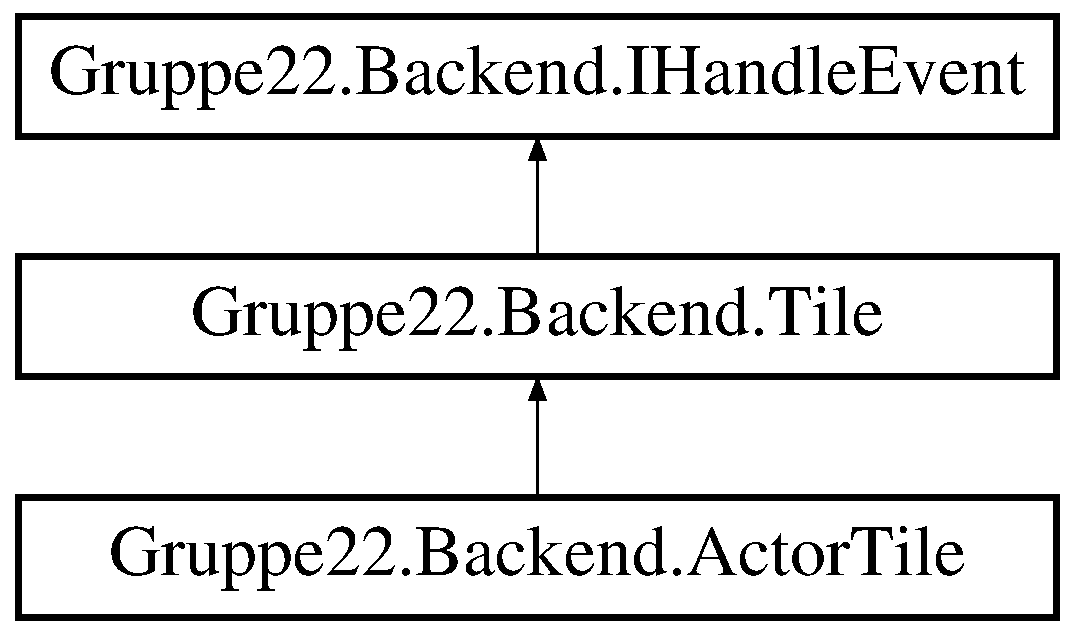
\includegraphics[height=3.000000cm]{class_gruppe22_1_1_backend_1_1_actor_tile}
\end{center}
\end{figure}
\subsection*{Öffentliche Methoden}
\begin{DoxyCompactItemize}
\item 
override void \hyperlink{class_gruppe22_1_1_backend_1_1_actor_tile_aad98091f10ca75642d211c1a837141e4}{Save} (Xml\-Writer xmlw)
\begin{DoxyCompactList}\small\item\em Abstract method to save a tile in a X\-M\-L file \end{DoxyCompactList}\item 
\hyperlink{class_gruppe22_1_1_backend_1_1_actor_tile_a1cf18c7c4d72100e5c60288e5b339dce}{Actor\-Tile} (object \hyperlink{class_gruppe22_1_1_backend_1_1_tile_abc12933c70eb3a2ebbb2fde9f45c2632}{parent}, \hyperlink{class_gruppe22_1_1_backend_1_1_actor}{Actor} \hyperlink{class_gruppe22_1_1_backend_1_1_actor_tile_a77ed5b0b9c6dd777a4a6242d4f3b5447}{actor})
\item 
void \hyperlink{class_gruppe22_1_1_backend_1_1_actor_tile_ab195619cedce5db86ed45978a6522a18}{Drop\-Items} ()
\item 
async Task \hyperlink{class_gruppe22_1_1_backend_1_1_actor_tile_a6f14e702f9cba241925195d13c54e6e5}{Workout\-Moves} ()
\item 
async Task \hyperlink{class_gruppe22_1_1_backend_1_1_actor_tile_af8bb4de8899a0b704b08e285efefed24}{Consider\-Moves} ()
\item 
override void \hyperlink{class_gruppe22_1_1_backend_1_1_actor_tile_a3e87be522214c2ab00966717c86f9af1}{Update} (Microsoft.\-Xna.\-Framework.\-Game\-Time game\-Time)
\item 
\hyperlink{class_gruppe22_1_1_backend_1_1_actor_tile_a9cb65b2c7c2c76fd2862bcc80f71c09d}{Actor\-Tile} (object \hyperlink{class_gruppe22_1_1_backend_1_1_tile_abc12933c70eb3a2ebbb2fde9f45c2632}{parent}, Random r=null)
\end{DoxyCompactItemize}
\subsection*{Propertys}
\begin{DoxyCompactItemize}
\item 
\hyperlink{class_gruppe22_1_1_backend_1_1_actor}{Actor} \hyperlink{class_gruppe22_1_1_backend_1_1_actor_tile_a77ed5b0b9c6dd777a4a6242d4f3b5447}{actor}\hspace{0.3cm}{\ttfamily  \mbox{[}get\mbox{]}}
\item 
\hyperlink{namespace_gruppe22_1_1_backend_a56d8f7bd1b5ba29d421c27a959523af3}{Actor\-Type} \hyperlink{class_gruppe22_1_1_backend_1_1_actor_tile_ab30c224f38c2e55d44d2cf65fe659f35}{actor\-Type}\hspace{0.3cm}{\ttfamily  \mbox{[}get\mbox{]}}
\item 
bool \hyperlink{class_gruppe22_1_1_backend_1_1_actor_tile_af8631f09f32bba5be31d3603b3df99c6}{enabled}\hspace{0.3cm}{\ttfamily  \mbox{[}get, set\mbox{]}}
\end{DoxyCompactItemize}
\subsection*{Weitere Geerbte Elemente}


\subsection{Beschreibung der Konstruktoren und Destruktoren}
\hypertarget{class_gruppe22_1_1_backend_1_1_actor_tile_a1cf18c7c4d72100e5c60288e5b339dce}{\index{Gruppe22\-::\-Backend\-::\-Actor\-Tile@{Gruppe22\-::\-Backend\-::\-Actor\-Tile}!Actor\-Tile@{Actor\-Tile}}
\index{Actor\-Tile@{Actor\-Tile}!Gruppe22::Backend::ActorTile@{Gruppe22\-::\-Backend\-::\-Actor\-Tile}}
\subsubsection[{Actor\-Tile}]{\setlength{\rightskip}{0pt plus 5cm}Gruppe22.\-Backend.\-Actor\-Tile.\-Actor\-Tile (
\begin{DoxyParamCaption}
\item[{object}]{parent, }
\item[{{\bf Actor}}]{actor}
\end{DoxyParamCaption}
)}}\label{class_gruppe22_1_1_backend_1_1_actor_tile_a1cf18c7c4d72100e5c60288e5b339dce}
\hypertarget{class_gruppe22_1_1_backend_1_1_actor_tile_a9cb65b2c7c2c76fd2862bcc80f71c09d}{\index{Gruppe22\-::\-Backend\-::\-Actor\-Tile@{Gruppe22\-::\-Backend\-::\-Actor\-Tile}!Actor\-Tile@{Actor\-Tile}}
\index{Actor\-Tile@{Actor\-Tile}!Gruppe22::Backend::ActorTile@{Gruppe22\-::\-Backend\-::\-Actor\-Tile}}
\subsubsection[{Actor\-Tile}]{\setlength{\rightskip}{0pt plus 5cm}Gruppe22.\-Backend.\-Actor\-Tile.\-Actor\-Tile (
\begin{DoxyParamCaption}
\item[{object}]{parent, }
\item[{Random}]{r = {\ttfamily null}}
\end{DoxyParamCaption}
)}}\label{class_gruppe22_1_1_backend_1_1_actor_tile_a9cb65b2c7c2c76fd2862bcc80f71c09d}


\subsection{Dokumentation der Elementfunktionen}
\hypertarget{class_gruppe22_1_1_backend_1_1_actor_tile_af8bb4de8899a0b704b08e285efefed24}{\index{Gruppe22\-::\-Backend\-::\-Actor\-Tile@{Gruppe22\-::\-Backend\-::\-Actor\-Tile}!Consider\-Moves@{Consider\-Moves}}
\index{Consider\-Moves@{Consider\-Moves}!Gruppe22::Backend::ActorTile@{Gruppe22\-::\-Backend\-::\-Actor\-Tile}}
\subsubsection[{Consider\-Moves}]{\setlength{\rightskip}{0pt plus 5cm}async Task Gruppe22.\-Backend.\-Actor\-Tile.\-Consider\-Moves (
\begin{DoxyParamCaption}
{}
\end{DoxyParamCaption}
)}}\label{class_gruppe22_1_1_backend_1_1_actor_tile_af8bb4de8899a0b704b08e285efefed24}
\hypertarget{class_gruppe22_1_1_backend_1_1_actor_tile_ab195619cedce5db86ed45978a6522a18}{\index{Gruppe22\-::\-Backend\-::\-Actor\-Tile@{Gruppe22\-::\-Backend\-::\-Actor\-Tile}!Drop\-Items@{Drop\-Items}}
\index{Drop\-Items@{Drop\-Items}!Gruppe22::Backend::ActorTile@{Gruppe22\-::\-Backend\-::\-Actor\-Tile}}
\subsubsection[{Drop\-Items}]{\setlength{\rightskip}{0pt plus 5cm}void Gruppe22.\-Backend.\-Actor\-Tile.\-Drop\-Items (
\begin{DoxyParamCaption}
{}
\end{DoxyParamCaption}
)}}\label{class_gruppe22_1_1_backend_1_1_actor_tile_ab195619cedce5db86ed45978a6522a18}
\hypertarget{class_gruppe22_1_1_backend_1_1_actor_tile_aad98091f10ca75642d211c1a837141e4}{\index{Gruppe22\-::\-Backend\-::\-Actor\-Tile@{Gruppe22\-::\-Backend\-::\-Actor\-Tile}!Save@{Save}}
\index{Save@{Save}!Gruppe22::Backend::ActorTile@{Gruppe22\-::\-Backend\-::\-Actor\-Tile}}
\subsubsection[{Save}]{\setlength{\rightskip}{0pt plus 5cm}override void Gruppe22.\-Backend.\-Actor\-Tile.\-Save (
\begin{DoxyParamCaption}
\item[{Xml\-Writer}]{xmlw}
\end{DoxyParamCaption}
)\hspace{0.3cm}{\ttfamily [virtual]}}}\label{class_gruppe22_1_1_backend_1_1_actor_tile_aad98091f10ca75642d211c1a837141e4}


Abstract method to save a tile in a X\-M\-L file 


\begin{DoxyParams}{Parameter}
{\em xmlw} & the Xml\-Writer used for saving the file\\
\hline
\end{DoxyParams}


Erneute Implementation von \hyperlink{class_gruppe22_1_1_backend_1_1_tile_a109ab3e77ffca9d44c95a711af3491dc}{Gruppe22.\-Backend.\-Tile}.

\hypertarget{class_gruppe22_1_1_backend_1_1_actor_tile_a3e87be522214c2ab00966717c86f9af1}{\index{Gruppe22\-::\-Backend\-::\-Actor\-Tile@{Gruppe22\-::\-Backend\-::\-Actor\-Tile}!Update@{Update}}
\index{Update@{Update}!Gruppe22::Backend::ActorTile@{Gruppe22\-::\-Backend\-::\-Actor\-Tile}}
\subsubsection[{Update}]{\setlength{\rightskip}{0pt plus 5cm}override void Gruppe22.\-Backend.\-Actor\-Tile.\-Update (
\begin{DoxyParamCaption}
\item[{Microsoft.\-Xna.\-Framework.\-Game\-Time}]{game\-Time}
\end{DoxyParamCaption}
)}}\label{class_gruppe22_1_1_backend_1_1_actor_tile_a3e87be522214c2ab00966717c86f9af1}
\hypertarget{class_gruppe22_1_1_backend_1_1_actor_tile_a6f14e702f9cba241925195d13c54e6e5}{\index{Gruppe22\-::\-Backend\-::\-Actor\-Tile@{Gruppe22\-::\-Backend\-::\-Actor\-Tile}!Workout\-Moves@{Workout\-Moves}}
\index{Workout\-Moves@{Workout\-Moves}!Gruppe22::Backend::ActorTile@{Gruppe22\-::\-Backend\-::\-Actor\-Tile}}
\subsubsection[{Workout\-Moves}]{\setlength{\rightskip}{0pt plus 5cm}async Task Gruppe22.\-Backend.\-Actor\-Tile.\-Workout\-Moves (
\begin{DoxyParamCaption}
{}
\end{DoxyParamCaption}
)}}\label{class_gruppe22_1_1_backend_1_1_actor_tile_a6f14e702f9cba241925195d13c54e6e5}


\subsection{Dokumentation der Propertys}
\hypertarget{class_gruppe22_1_1_backend_1_1_actor_tile_a77ed5b0b9c6dd777a4a6242d4f3b5447}{\index{Gruppe22\-::\-Backend\-::\-Actor\-Tile@{Gruppe22\-::\-Backend\-::\-Actor\-Tile}!actor@{actor}}
\index{actor@{actor}!Gruppe22::Backend::ActorTile@{Gruppe22\-::\-Backend\-::\-Actor\-Tile}}
\subsubsection[{actor}]{\setlength{\rightskip}{0pt plus 5cm}{\bf Actor} Gruppe22.\-Backend.\-Actor\-Tile.\-actor\hspace{0.3cm}{\ttfamily [get]}}}\label{class_gruppe22_1_1_backend_1_1_actor_tile_a77ed5b0b9c6dd777a4a6242d4f3b5447}
\hypertarget{class_gruppe22_1_1_backend_1_1_actor_tile_ab30c224f38c2e55d44d2cf65fe659f35}{\index{Gruppe22\-::\-Backend\-::\-Actor\-Tile@{Gruppe22\-::\-Backend\-::\-Actor\-Tile}!actor\-Type@{actor\-Type}}
\index{actor\-Type@{actor\-Type}!Gruppe22::Backend::ActorTile@{Gruppe22\-::\-Backend\-::\-Actor\-Tile}}
\subsubsection[{actor\-Type}]{\setlength{\rightskip}{0pt plus 5cm}{\bf Actor\-Type} Gruppe22.\-Backend.\-Actor\-Tile.\-actor\-Type\hspace{0.3cm}{\ttfamily [get]}}}\label{class_gruppe22_1_1_backend_1_1_actor_tile_ab30c224f38c2e55d44d2cf65fe659f35}
\hypertarget{class_gruppe22_1_1_backend_1_1_actor_tile_af8631f09f32bba5be31d3603b3df99c6}{\index{Gruppe22\-::\-Backend\-::\-Actor\-Tile@{Gruppe22\-::\-Backend\-::\-Actor\-Tile}!enabled@{enabled}}
\index{enabled@{enabled}!Gruppe22::Backend::ActorTile@{Gruppe22\-::\-Backend\-::\-Actor\-Tile}}
\subsubsection[{enabled}]{\setlength{\rightskip}{0pt plus 5cm}bool Gruppe22.\-Backend.\-Actor\-Tile.\-enabled\hspace{0.3cm}{\ttfamily [get]}, {\ttfamily [set]}}}\label{class_gruppe22_1_1_backend_1_1_actor_tile_af8631f09f32bba5be31d3603b3df99c6}


Die Dokumentation für diese Klasse wurde erzeugt aufgrund der Datei\-:\begin{DoxyCompactItemize}
\item 
C\-:/\-Users/beursken/\-Documents/\-Git\-Hub/gruppe22/\-Gruppe22/\-Gruppe22/\-Backend/\-Map/\hyperlink{_actor_tile_8cs}{Actor\-Tile.\-cs}\end{DoxyCompactItemize}

\hypertarget{class_gruppe22_1_1_client_1_1_actor_view}{\section{Gruppe22.\-Client.\-Actor\-View Klassenreferenz}
\label{class_gruppe22_1_1_client_1_1_actor_view}\index{Gruppe22.\-Client.\-Actor\-View@{Gruppe22.\-Client.\-Actor\-View}}
}
Klassendiagramm für Gruppe22.\-Client.\-Actor\-View\-:\begin{figure}[H]
\begin{center}
\leavevmode
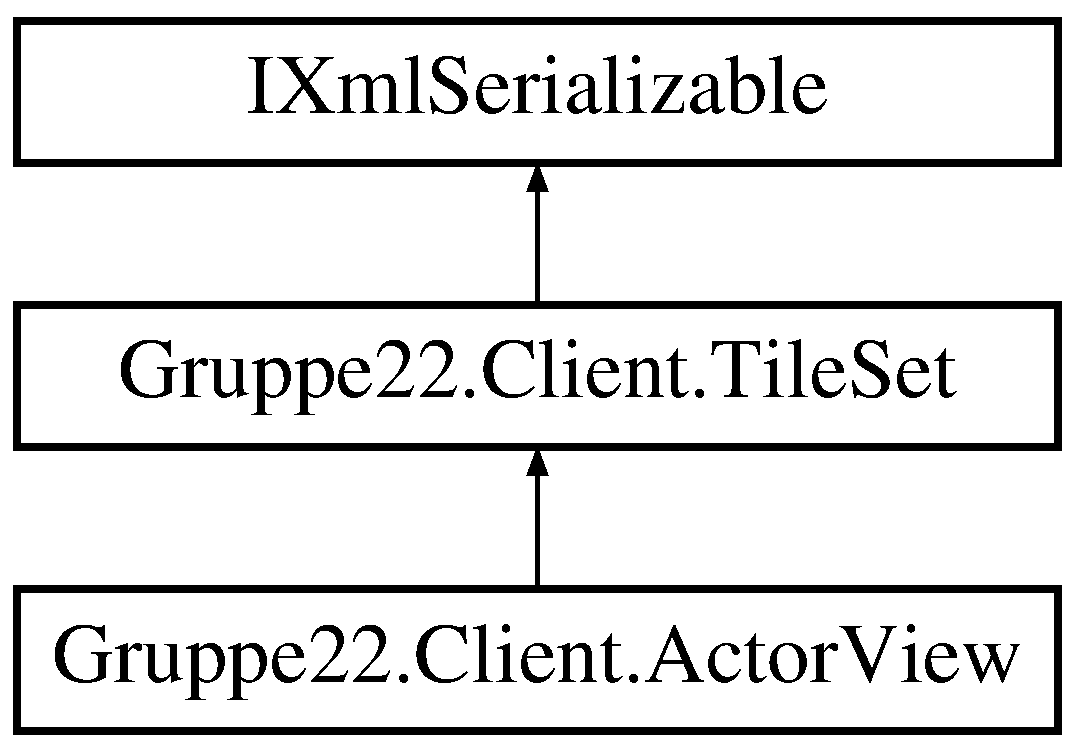
\includegraphics[height=3.000000cm]{class_gruppe22_1_1_client_1_1_actor_view}
\end{center}
\end{figure}
\subsection*{Öffentliche Methoden}
\begin{DoxyCompactItemize}
\item 
void \hyperlink{class_gruppe22_1_1_client_1_1_actor_view_af0bf5a4427fcaf23ac0af9f286f246e1}{Play\-Now\-Or\-After\-Move} (\hyperlink{namespace_gruppe22_1_1_backend_aaa25d27da5307e9abb21f9f09b528f67}{Backend.\-Activity} \hyperlink{class_gruppe22_1_1_client_1_1_actor_view_af7f1f3741a7266476953b693df0067a2}{activity}, bool locked=false)
\item 
void \hyperlink{class_gruppe22_1_1_client_1_1_actor_view_a784d66744fea2c43f7a705c4bebb80a3}{End\-Move\-And\-Play} (\hyperlink{namespace_gruppe22_1_1_backend_aaa25d27da5307e9abb21f9f09b528f67}{Backend.\-Activity} \hyperlink{class_gruppe22_1_1_client_1_1_actor_view_af7f1f3741a7266476953b693df0067a2}{activity}, bool locked=false)
\item 
void \hyperlink{class_gruppe22_1_1_client_1_1_actor_view_abe6b2c58e6d9796f2a351af99689c9db}{Kill} ()
\begin{DoxyCompactList}\small\item\em Sets an actor to \char`\"{}dead\char`\"{} state and displays final frame of animation \end{DoxyCompactList}\item 
override void \hyperlink{class_gruppe22_1_1_client_1_1_actor_view_a1b068bd49a64ea380d700155ec9bda5e}{Read\-Xml} (System.\-Xml.\-Xml\-Reader reader)
\begin{DoxyCompactList}\small\item\em Load object from X\-M\-L-\/file \end{DoxyCompactList}\item 
override void \hyperlink{class_gruppe22_1_1_client_1_1_actor_view_a18566b8e88b63aa9901be779ebde09ab}{Save} (string \hyperlink{class_gruppe22_1_1_client_1_1_tile_set_afce49a3941b2d4a360990f9847282da1}{filename}=\char`\"{}bla.\-xml\char`\"{})
\begin{DoxyCompactList}\small\item\em Save (merely a shortcut to the serializer \end{DoxyCompactList}\item 
override void \hyperlink{class_gruppe22_1_1_client_1_1_actor_view_af94fec8c50c0919b4c762df7c681db4b}{Load} (string \hyperlink{class_gruppe22_1_1_client_1_1_tile_set_afce49a3941b2d4a360990f9847282da1}{filename}=\char`\"{}bla.\-xml\char`\"{})
\begin{DoxyCompactList}\small\item\em Load (cannot use serializer at this level!) \end{DoxyCompactList}\item 
override void \hyperlink{class_gruppe22_1_1_client_1_1_actor_view_af04d89d3988da620d7b092055f64b37b}{Write\-Xml} (System.\-Xml.\-Xml\-Writer writer)
\begin{DoxyCompactList}\small\item\em Dump object to X\-M\-L-\/file \end{DoxyCompactList}\item 
void \hyperlink{class_gruppe22_1_1_client_1_1_actor_view_ae79845d8f30b5eaae104757b85043386}{Add} (\hyperlink{namespace_gruppe22_1_1_backend_aaa25d27da5307e9abb21f9f09b528f67}{Backend.\-Activity} \hyperlink{class_gruppe22_1_1_client_1_1_actor_view_af7f1f3741a7266476953b693df0067a2}{activity}, \hyperlink{namespace_gruppe22_1_1_backend_a2d53d5d14b8ea0951ba6971e5da1ebf5}{Backend.\-Direction} \hyperlink{class_gruppe22_1_1_client_1_1_actor_view_ad51208acd18670716bde6c746b86655b}{direction}, string \hyperlink{class_gruppe22_1_1_client_1_1_tile_set_afce49a3941b2d4a360990f9847282da1}{filename}, \hyperlink{class_gruppe22_1_1_backend_1_1_coords}{Backend.\-Coords} start\-Pos, int cols=1, int rows=1, \hyperlink{class_gruppe22_1_1_backend_1_1_coords}{Backend.\-Coords} offset=null, \hyperlink{class_gruppe22_1_1_backend_1_1_coords}{Backend.\-Coords} crop=null, bool vertical=false)
\begin{DoxyCompactList}\small\item\em Add animation for certain activity from a file \end{DoxyCompactList}\item 
void \hyperlink{class_gruppe22_1_1_client_1_1_actor_view_aa5ff2045ed28649dfe11428be9c39660}{Animate} (bool has\-Moved)
\item 
void \hyperlink{class_gruppe22_1_1_client_1_1_actor_view_ae9b9945e735d77eba0a5118bcbb93596}{Update} (Game\-Time gametime)
\item 
\hyperlink{class_gruppe22_1_1_client_1_1_actor_view_a84160789d74c4206e3adbf18078c62a8}{Actor\-View} ()
\item 
\hyperlink{class_gruppe22_1_1_client_1_1_actor_view_a7a97196d62da28a51d533aa167e00c2f}{Actor\-View} (\hyperlink{class_gruppe22_1_1_client_1_1_camera}{Camera} camera, \hyperlink{interface_gruppe22_1_1_backend_1_1_i_handle_event}{Backend.\-I\-Handle\-Event} parent, int \hyperlink{class_gruppe22_1_1_client_1_1_actor_view_a6468d36affd0a3d63e3873cb201c4b3e}{id}, Content\-Manager content, \hyperlink{class_gruppe22_1_1_backend_1_1_coords}{Backend.\-Coords} \hyperlink{class_gruppe22_1_1_client_1_1_actor_view_a5a4e1de85966801e99c5fb08f7d342ca}{position}, string \hyperlink{class_gruppe22_1_1_client_1_1_tile_set_afce49a3941b2d4a360990f9847282da1}{filename}=\char`\"{}\char`\"{}, int \hyperlink{class_gruppe22_1_1_client_1_1_actor_view_a3c41306652c4ca9d9ab01b32445ce7da}{speed}=5, bool alive=true, int \hyperlink{class_gruppe22_1_1_client_1_1_tile_set_aff0371f9e4071f24de16612c2066ad5b}{width}=96, int \hyperlink{class_gruppe22_1_1_client_1_1_tile_set_a12343c861014c3631e1a40dfeef20312}{height}=96)
\end{DoxyCompactItemize}
\subsection*{Propertys}
\begin{DoxyCompactItemize}
\item 
\hyperlink{class_gruppe22_1_1_client_1_1_map_effect}{Map\-Effect} \hyperlink{class_gruppe22_1_1_client_1_1_actor_view_abb2c41d338d432d46f77f3ba2a41cfca}{effect}\hspace{0.3cm}{\ttfamily  \mbox{[}get, set\mbox{]}}
\item 
\hyperlink{class_gruppe22_1_1_backend_1_1_coords}{Backend.\-Coords} \hyperlink{class_gruppe22_1_1_client_1_1_actor_view_a5a4e1de85966801e99c5fb08f7d342ca}{position}\hspace{0.3cm}{\ttfamily  \mbox{[}get, set\mbox{]}}
\item 
int \hyperlink{class_gruppe22_1_1_client_1_1_actor_view_a6468d36affd0a3d63e3873cb201c4b3e}{id}\hspace{0.3cm}{\ttfamily  \mbox{[}get\mbox{]}}
\item 
int \hyperlink{class_gruppe22_1_1_client_1_1_actor_view_a3c41306652c4ca9d9ab01b32445ce7da}{speed}\hspace{0.3cm}{\ttfamily  \mbox{[}get, set\mbox{]}}
\item 
\hyperlink{class_gruppe22_1_1_backend_1_1_coords}{Backend.\-Coords} \hyperlink{class_gruppe22_1_1_client_1_1_actor_view_a0797749459b19b816824f63199eb3345}{target}\hspace{0.3cm}{\ttfamily  \mbox{[}get, set\mbox{]}}
\item 
\hyperlink{class_gruppe22_1_1_backend_1_1_coords}{Backend.\-Coords} \hyperlink{class_gruppe22_1_1_client_1_1_actor_view_af45fbf7af164d290ea08e1091f8b4359}{cache\-Target}\hspace{0.3cm}{\ttfamily  \mbox{[}set\mbox{]}}
\item 
\hyperlink{namespace_gruppe22_1_1_backend_a2d53d5d14b8ea0951ba6971e5da1ebf5}{Backend.\-Direction} \hyperlink{class_gruppe22_1_1_client_1_1_actor_view_a892ab20788c4b8f17d7cb945a4c82cb2}{cache\-Dir}\hspace{0.3cm}{\ttfamily  \mbox{[}get, set\mbox{]}}
\item 
bool \hyperlink{class_gruppe22_1_1_client_1_1_actor_view_a7fb53fb0eb252d2b67410f9f9eae683c}{is\-Moving}\hspace{0.3cm}{\ttfamily  \mbox{[}get\mbox{]}}
\item 
\hyperlink{namespace_gruppe22_1_1_backend_aaa25d27da5307e9abb21f9f09b528f67}{Backend.\-Activity} \hyperlink{class_gruppe22_1_1_client_1_1_actor_view_af7f1f3741a7266476953b693df0067a2}{activity}\hspace{0.3cm}{\ttfamily  \mbox{[}get, set\mbox{]}}
\item 
\hyperlink{namespace_gruppe22_1_1_backend_a2d53d5d14b8ea0951ba6971e5da1ebf5}{Backend.\-Direction} \hyperlink{class_gruppe22_1_1_client_1_1_actor_view_ad51208acd18670716bde6c746b86655b}{direction}\hspace{0.3cm}{\ttfamily  \mbox{[}get, set\mbox{]}}
\item 
Texture2\-D \hyperlink{class_gruppe22_1_1_client_1_1_actor_view_a05942cdc958c646c23de2c6327bd7f54}{animation\-Texture}\hspace{0.3cm}{\ttfamily  \mbox{[}get\mbox{]}}
\item 
Rectangle \hyperlink{class_gruppe22_1_1_client_1_1_actor_view_ac447bd2a93cd5e534ff446d0244bca63}{animation\-Rect}\hspace{0.3cm}{\ttfamily  \mbox{[}get\mbox{]}}
\item 
int \hyperlink{class_gruppe22_1_1_client_1_1_actor_view_a9a4c4ec1dc5769d84653c1d41c4cf4dd}{offset\-Y}\hspace{0.3cm}{\ttfamily  \mbox{[}get\mbox{]}}
\item 
int \hyperlink{class_gruppe22_1_1_client_1_1_actor_view_a1786159bc34dd01c8390b493937df033}{offset\-X}\hspace{0.3cm}{\ttfamily  \mbox{[}get, set\mbox{]}}
\item 
int \hyperlink{class_gruppe22_1_1_client_1_1_actor_view_add6a5e3e2f6769eccff26a3d5ea0ef58}{crop\-X}\hspace{0.3cm}{\ttfamily  \mbox{[}get, set\mbox{]}}
\item 
int \hyperlink{class_gruppe22_1_1_client_1_1_actor_view_aa61c6d089ffd6ac7170dd2a6375ef85e}{crop\-Y}\hspace{0.3cm}{\ttfamily  \mbox{[}get, set\mbox{]}}
\end{DoxyCompactItemize}
\subsection*{Weitere Geerbte Elemente}


\subsection{Beschreibung der Konstruktoren und Destruktoren}
\hypertarget{class_gruppe22_1_1_client_1_1_actor_view_a84160789d74c4206e3adbf18078c62a8}{\index{Gruppe22\-::\-Client\-::\-Actor\-View@{Gruppe22\-::\-Client\-::\-Actor\-View}!Actor\-View@{Actor\-View}}
\index{Actor\-View@{Actor\-View}!Gruppe22::Client::ActorView@{Gruppe22\-::\-Client\-::\-Actor\-View}}
\subsubsection[{Actor\-View}]{\setlength{\rightskip}{0pt plus 5cm}Gruppe22.\-Client.\-Actor\-View.\-Actor\-View (
\begin{DoxyParamCaption}
{}
\end{DoxyParamCaption}
)}}\label{class_gruppe22_1_1_client_1_1_actor_view_a84160789d74c4206e3adbf18078c62a8}
\hypertarget{class_gruppe22_1_1_client_1_1_actor_view_a7a97196d62da28a51d533aa167e00c2f}{\index{Gruppe22\-::\-Client\-::\-Actor\-View@{Gruppe22\-::\-Client\-::\-Actor\-View}!Actor\-View@{Actor\-View}}
\index{Actor\-View@{Actor\-View}!Gruppe22::Client::ActorView@{Gruppe22\-::\-Client\-::\-Actor\-View}}
\subsubsection[{Actor\-View}]{\setlength{\rightskip}{0pt plus 5cm}Gruppe22.\-Client.\-Actor\-View.\-Actor\-View (
\begin{DoxyParamCaption}
\item[{{\bf Camera}}]{camera, }
\item[{{\bf Backend.\-I\-Handle\-Event}}]{parent, }
\item[{int}]{id, }
\item[{Content\-Manager}]{content, }
\item[{{\bf Backend.\-Coords}}]{position, }
\item[{string}]{filename = {\ttfamily \char`\"{}\char`\"{}}, }
\item[{int}]{speed = {\ttfamily 5}, }
\item[{bool}]{alive = {\ttfamily true}, }
\item[{int}]{width = {\ttfamily 96}, }
\item[{int}]{height = {\ttfamily 96}}
\end{DoxyParamCaption}
)}}\label{class_gruppe22_1_1_client_1_1_actor_view_a7a97196d62da28a51d533aa167e00c2f}





\begin{DoxyParams}{Parameter}
{\em spritebatch} & \\
\hline
{\em name} & \\
\hline
{\em controllable} & \\
\hline
{\em position} & \\
\hline
{\em sprite} & \\
\hline
\end{DoxyParams}


\subsection{Dokumentation der Elementfunktionen}
\hypertarget{class_gruppe22_1_1_client_1_1_actor_view_ae79845d8f30b5eaae104757b85043386}{\index{Gruppe22\-::\-Client\-::\-Actor\-View@{Gruppe22\-::\-Client\-::\-Actor\-View}!Add@{Add}}
\index{Add@{Add}!Gruppe22::Client::ActorView@{Gruppe22\-::\-Client\-::\-Actor\-View}}
\subsubsection[{Add}]{\setlength{\rightskip}{0pt plus 5cm}void Gruppe22.\-Client.\-Actor\-View.\-Add (
\begin{DoxyParamCaption}
\item[{{\bf Backend.\-Activity}}]{activity, }
\item[{{\bf Backend.\-Direction}}]{direction, }
\item[{string}]{filename, }
\item[{{\bf Backend.\-Coords}}]{start\-Pos, }
\item[{int}]{cols = {\ttfamily 1}, }
\item[{int}]{rows = {\ttfamily 1}, }
\item[{{\bf Backend.\-Coords}}]{offset = {\ttfamily null}, }
\item[{{\bf Backend.\-Coords}}]{crop = {\ttfamily null}, }
\item[{bool}]{vertical = {\ttfamily false}}
\end{DoxyParamCaption}
)}}\label{class_gruppe22_1_1_client_1_1_actor_view_ae79845d8f30b5eaae104757b85043386}


Add animation for certain activity from a file 


\begin{DoxyParams}{Parameter}
{\em activity} & \\
\hline
{\em direction} & \\
\hline
{\em filename} & \\
\hline
{\em start\-Pos} & \\
\hline
{\em cols} & \\
\hline
{\em rows} & \\
\hline
{\em vertical} & \\
\hline
\end{DoxyParams}
\hypertarget{class_gruppe22_1_1_client_1_1_actor_view_aa5ff2045ed28649dfe11428be9c39660}{\index{Gruppe22\-::\-Client\-::\-Actor\-View@{Gruppe22\-::\-Client\-::\-Actor\-View}!Animate@{Animate}}
\index{Animate@{Animate}!Gruppe22::Client::ActorView@{Gruppe22\-::\-Client\-::\-Actor\-View}}
\subsubsection[{Animate}]{\setlength{\rightskip}{0pt plus 5cm}void Gruppe22.\-Client.\-Actor\-View.\-Animate (
\begin{DoxyParamCaption}
\item[{bool}]{has\-Moved}
\end{DoxyParamCaption}
)}}\label{class_gruppe22_1_1_client_1_1_actor_view_aa5ff2045ed28649dfe11428be9c39660}
\hypertarget{class_gruppe22_1_1_client_1_1_actor_view_a784d66744fea2c43f7a705c4bebb80a3}{\index{Gruppe22\-::\-Client\-::\-Actor\-View@{Gruppe22\-::\-Client\-::\-Actor\-View}!End\-Move\-And\-Play@{End\-Move\-And\-Play}}
\index{End\-Move\-And\-Play@{End\-Move\-And\-Play}!Gruppe22::Client::ActorView@{Gruppe22\-::\-Client\-::\-Actor\-View}}
\subsubsection[{End\-Move\-And\-Play}]{\setlength{\rightskip}{0pt plus 5cm}void Gruppe22.\-Client.\-Actor\-View.\-End\-Move\-And\-Play (
\begin{DoxyParamCaption}
\item[{{\bf Backend.\-Activity}}]{activity, }
\item[{bool}]{locked = {\ttfamily false}}
\end{DoxyParamCaption}
)}}\label{class_gruppe22_1_1_client_1_1_actor_view_a784d66744fea2c43f7a705c4bebb80a3}
\hypertarget{class_gruppe22_1_1_client_1_1_actor_view_abe6b2c58e6d9796f2a351af99689c9db}{\index{Gruppe22\-::\-Client\-::\-Actor\-View@{Gruppe22\-::\-Client\-::\-Actor\-View}!Kill@{Kill}}
\index{Kill@{Kill}!Gruppe22::Client::ActorView@{Gruppe22\-::\-Client\-::\-Actor\-View}}
\subsubsection[{Kill}]{\setlength{\rightskip}{0pt plus 5cm}void Gruppe22.\-Client.\-Actor\-View.\-Kill (
\begin{DoxyParamCaption}
{}
\end{DoxyParamCaption}
)}}\label{class_gruppe22_1_1_client_1_1_actor_view_abe6b2c58e6d9796f2a351af99689c9db}


Sets an actor to \char`\"{}dead\char`\"{} state and displays final frame of animation 

\hypertarget{class_gruppe22_1_1_client_1_1_actor_view_af94fec8c50c0919b4c762df7c681db4b}{\index{Gruppe22\-::\-Client\-::\-Actor\-View@{Gruppe22\-::\-Client\-::\-Actor\-View}!Load@{Load}}
\index{Load@{Load}!Gruppe22::Client::ActorView@{Gruppe22\-::\-Client\-::\-Actor\-View}}
\subsubsection[{Load}]{\setlength{\rightskip}{0pt plus 5cm}override void Gruppe22.\-Client.\-Actor\-View.\-Load (
\begin{DoxyParamCaption}
\item[{string}]{filename = {\ttfamily \char`\"{}bla.xml\char`\"{}}}
\end{DoxyParamCaption}
)\hspace{0.3cm}{\ttfamily [virtual]}}}\label{class_gruppe22_1_1_client_1_1_actor_view_af94fec8c50c0919b4c762df7c681db4b}


Load (cannot use serializer at this level!) 


\begin{DoxyParams}{Parameter}
{\em filename} & \\
\hline
\end{DoxyParams}


Erneute Implementation von \hyperlink{class_gruppe22_1_1_client_1_1_tile_set_a9dd72fa07af2de21ab5c68e9d63c83f2}{Gruppe22.\-Client.\-Tile\-Set}.

\hypertarget{class_gruppe22_1_1_client_1_1_actor_view_af0bf5a4427fcaf23ac0af9f286f246e1}{\index{Gruppe22\-::\-Client\-::\-Actor\-View@{Gruppe22\-::\-Client\-::\-Actor\-View}!Play\-Now\-Or\-After\-Move@{Play\-Now\-Or\-After\-Move}}
\index{Play\-Now\-Or\-After\-Move@{Play\-Now\-Or\-After\-Move}!Gruppe22::Client::ActorView@{Gruppe22\-::\-Client\-::\-Actor\-View}}
\subsubsection[{Play\-Now\-Or\-After\-Move}]{\setlength{\rightskip}{0pt plus 5cm}void Gruppe22.\-Client.\-Actor\-View.\-Play\-Now\-Or\-After\-Move (
\begin{DoxyParamCaption}
\item[{{\bf Backend.\-Activity}}]{activity, }
\item[{bool}]{locked = {\ttfamily false}}
\end{DoxyParamCaption}
)}}\label{class_gruppe22_1_1_client_1_1_actor_view_af0bf5a4427fcaf23ac0af9f286f246e1}
\hypertarget{class_gruppe22_1_1_client_1_1_actor_view_a1b068bd49a64ea380d700155ec9bda5e}{\index{Gruppe22\-::\-Client\-::\-Actor\-View@{Gruppe22\-::\-Client\-::\-Actor\-View}!Read\-Xml@{Read\-Xml}}
\index{Read\-Xml@{Read\-Xml}!Gruppe22::Client::ActorView@{Gruppe22\-::\-Client\-::\-Actor\-View}}
\subsubsection[{Read\-Xml}]{\setlength{\rightskip}{0pt plus 5cm}override void Gruppe22.\-Client.\-Actor\-View.\-Read\-Xml (
\begin{DoxyParamCaption}
\item[{System.\-Xml.\-Xml\-Reader}]{reader}
\end{DoxyParamCaption}
)\hspace{0.3cm}{\ttfamily [virtual]}}}\label{class_gruppe22_1_1_client_1_1_actor_view_a1b068bd49a64ea380d700155ec9bda5e}


Load object from X\-M\-L-\/file 


\begin{DoxyParams}{Parameter}
{\em reader} & Load object from X\-M\-L-\/stream\\
\hline
\end{DoxyParams}


Erneute Implementation von \hyperlink{class_gruppe22_1_1_client_1_1_tile_set_a7395745bf6ef4bf3374d4221cb86689f}{Gruppe22.\-Client.\-Tile\-Set}.

\hypertarget{class_gruppe22_1_1_client_1_1_actor_view_a18566b8e88b63aa9901be779ebde09ab}{\index{Gruppe22\-::\-Client\-::\-Actor\-View@{Gruppe22\-::\-Client\-::\-Actor\-View}!Save@{Save}}
\index{Save@{Save}!Gruppe22::Client::ActorView@{Gruppe22\-::\-Client\-::\-Actor\-View}}
\subsubsection[{Save}]{\setlength{\rightskip}{0pt plus 5cm}override void Gruppe22.\-Client.\-Actor\-View.\-Save (
\begin{DoxyParamCaption}
\item[{string}]{filename = {\ttfamily \char`\"{}bla.xml\char`\"{}}}
\end{DoxyParamCaption}
)\hspace{0.3cm}{\ttfamily [virtual]}}}\label{class_gruppe22_1_1_client_1_1_actor_view_a18566b8e88b63aa9901be779ebde09ab}


Save (merely a shortcut to the serializer 


\begin{DoxyParams}{Parameter}
{\em filename} & \\
\hline
\end{DoxyParams}


Erneute Implementation von \hyperlink{class_gruppe22_1_1_client_1_1_tile_set_aee5a346f67239555aabd55180b29c10f}{Gruppe22.\-Client.\-Tile\-Set}.

\hypertarget{class_gruppe22_1_1_client_1_1_actor_view_ae9b9945e735d77eba0a5118bcbb93596}{\index{Gruppe22\-::\-Client\-::\-Actor\-View@{Gruppe22\-::\-Client\-::\-Actor\-View}!Update@{Update}}
\index{Update@{Update}!Gruppe22::Client::ActorView@{Gruppe22\-::\-Client\-::\-Actor\-View}}
\subsubsection[{Update}]{\setlength{\rightskip}{0pt plus 5cm}void Gruppe22.\-Client.\-Actor\-View.\-Update (
\begin{DoxyParamCaption}
\item[{Game\-Time}]{gametime}
\end{DoxyParamCaption}
)}}\label{class_gruppe22_1_1_client_1_1_actor_view_ae9b9945e735d77eba0a5118bcbb93596}





\begin{DoxyParams}{Parameter}
{\em gametime} & \\
\hline
\end{DoxyParams}
\hypertarget{class_gruppe22_1_1_client_1_1_actor_view_af04d89d3988da620d7b092055f64b37b}{\index{Gruppe22\-::\-Client\-::\-Actor\-View@{Gruppe22\-::\-Client\-::\-Actor\-View}!Write\-Xml@{Write\-Xml}}
\index{Write\-Xml@{Write\-Xml}!Gruppe22::Client::ActorView@{Gruppe22\-::\-Client\-::\-Actor\-View}}
\subsubsection[{Write\-Xml}]{\setlength{\rightskip}{0pt plus 5cm}override void Gruppe22.\-Client.\-Actor\-View.\-Write\-Xml (
\begin{DoxyParamCaption}
\item[{System.\-Xml.\-Xml\-Writer}]{writer}
\end{DoxyParamCaption}
)\hspace{0.3cm}{\ttfamily [virtual]}}}\label{class_gruppe22_1_1_client_1_1_actor_view_af04d89d3988da620d7b092055f64b37b}


Dump object to X\-M\-L-\/file 


\begin{DoxyParams}{Parameter}
{\em writer} & Write object to X\-M\-L-\/stream\\
\hline
\end{DoxyParams}


Erneute Implementation von \hyperlink{class_gruppe22_1_1_client_1_1_tile_set_a4a27a9d327257a79db59b2681daaa0c7}{Gruppe22.\-Client.\-Tile\-Set}.



\subsection{Dokumentation der Propertys}
\hypertarget{class_gruppe22_1_1_client_1_1_actor_view_af7f1f3741a7266476953b693df0067a2}{\index{Gruppe22\-::\-Client\-::\-Actor\-View@{Gruppe22\-::\-Client\-::\-Actor\-View}!activity@{activity}}
\index{activity@{activity}!Gruppe22::Client::ActorView@{Gruppe22\-::\-Client\-::\-Actor\-View}}
\subsubsection[{activity}]{\setlength{\rightskip}{0pt plus 5cm}{\bf Backend.\-Activity} Gruppe22.\-Client.\-Actor\-View.\-activity\hspace{0.3cm}{\ttfamily [get]}, {\ttfamily [set]}}}\label{class_gruppe22_1_1_client_1_1_actor_view_af7f1f3741a7266476953b693df0067a2}
\hypertarget{class_gruppe22_1_1_client_1_1_actor_view_ac447bd2a93cd5e534ff446d0244bca63}{\index{Gruppe22\-::\-Client\-::\-Actor\-View@{Gruppe22\-::\-Client\-::\-Actor\-View}!animation\-Rect@{animation\-Rect}}
\index{animation\-Rect@{animation\-Rect}!Gruppe22::Client::ActorView@{Gruppe22\-::\-Client\-::\-Actor\-View}}
\subsubsection[{animation\-Rect}]{\setlength{\rightskip}{0pt plus 5cm}Rectangle Gruppe22.\-Client.\-Actor\-View.\-animation\-Rect\hspace{0.3cm}{\ttfamily [get]}}}\label{class_gruppe22_1_1_client_1_1_actor_view_ac447bd2a93cd5e534ff446d0244bca63}
\hypertarget{class_gruppe22_1_1_client_1_1_actor_view_a05942cdc958c646c23de2c6327bd7f54}{\index{Gruppe22\-::\-Client\-::\-Actor\-View@{Gruppe22\-::\-Client\-::\-Actor\-View}!animation\-Texture@{animation\-Texture}}
\index{animation\-Texture@{animation\-Texture}!Gruppe22::Client::ActorView@{Gruppe22\-::\-Client\-::\-Actor\-View}}
\subsubsection[{animation\-Texture}]{\setlength{\rightskip}{0pt plus 5cm}Texture2\-D Gruppe22.\-Client.\-Actor\-View.\-animation\-Texture\hspace{0.3cm}{\ttfamily [get]}}}\label{class_gruppe22_1_1_client_1_1_actor_view_a05942cdc958c646c23de2c6327bd7f54}
\hypertarget{class_gruppe22_1_1_client_1_1_actor_view_a892ab20788c4b8f17d7cb945a4c82cb2}{\index{Gruppe22\-::\-Client\-::\-Actor\-View@{Gruppe22\-::\-Client\-::\-Actor\-View}!cache\-Dir@{cache\-Dir}}
\index{cache\-Dir@{cache\-Dir}!Gruppe22::Client::ActorView@{Gruppe22\-::\-Client\-::\-Actor\-View}}
\subsubsection[{cache\-Dir}]{\setlength{\rightskip}{0pt plus 5cm}{\bf Backend.\-Direction} Gruppe22.\-Client.\-Actor\-View.\-cache\-Dir\hspace{0.3cm}{\ttfamily [get]}, {\ttfamily [set]}}}\label{class_gruppe22_1_1_client_1_1_actor_view_a892ab20788c4b8f17d7cb945a4c82cb2}
\hypertarget{class_gruppe22_1_1_client_1_1_actor_view_af45fbf7af164d290ea08e1091f8b4359}{\index{Gruppe22\-::\-Client\-::\-Actor\-View@{Gruppe22\-::\-Client\-::\-Actor\-View}!cache\-Target@{cache\-Target}}
\index{cache\-Target@{cache\-Target}!Gruppe22::Client::ActorView@{Gruppe22\-::\-Client\-::\-Actor\-View}}
\subsubsection[{cache\-Target}]{\setlength{\rightskip}{0pt plus 5cm}{\bf Backend.\-Coords} Gruppe22.\-Client.\-Actor\-View.\-cache\-Target\hspace{0.3cm}{\ttfamily [set]}}}\label{class_gruppe22_1_1_client_1_1_actor_view_af45fbf7af164d290ea08e1091f8b4359}
\hypertarget{class_gruppe22_1_1_client_1_1_actor_view_add6a5e3e2f6769eccff26a3d5ea0ef58}{\index{Gruppe22\-::\-Client\-::\-Actor\-View@{Gruppe22\-::\-Client\-::\-Actor\-View}!crop\-X@{crop\-X}}
\index{crop\-X@{crop\-X}!Gruppe22::Client::ActorView@{Gruppe22\-::\-Client\-::\-Actor\-View}}
\subsubsection[{crop\-X}]{\setlength{\rightskip}{0pt plus 5cm}int Gruppe22.\-Client.\-Actor\-View.\-crop\-X\hspace{0.3cm}{\ttfamily [get]}, {\ttfamily [set]}}}\label{class_gruppe22_1_1_client_1_1_actor_view_add6a5e3e2f6769eccff26a3d5ea0ef58}
\hypertarget{class_gruppe22_1_1_client_1_1_actor_view_aa61c6d089ffd6ac7170dd2a6375ef85e}{\index{Gruppe22\-::\-Client\-::\-Actor\-View@{Gruppe22\-::\-Client\-::\-Actor\-View}!crop\-Y@{crop\-Y}}
\index{crop\-Y@{crop\-Y}!Gruppe22::Client::ActorView@{Gruppe22\-::\-Client\-::\-Actor\-View}}
\subsubsection[{crop\-Y}]{\setlength{\rightskip}{0pt plus 5cm}int Gruppe22.\-Client.\-Actor\-View.\-crop\-Y\hspace{0.3cm}{\ttfamily [get]}, {\ttfamily [set]}}}\label{class_gruppe22_1_1_client_1_1_actor_view_aa61c6d089ffd6ac7170dd2a6375ef85e}
\hypertarget{class_gruppe22_1_1_client_1_1_actor_view_ad51208acd18670716bde6c746b86655b}{\index{Gruppe22\-::\-Client\-::\-Actor\-View@{Gruppe22\-::\-Client\-::\-Actor\-View}!direction@{direction}}
\index{direction@{direction}!Gruppe22::Client::ActorView@{Gruppe22\-::\-Client\-::\-Actor\-View}}
\subsubsection[{direction}]{\setlength{\rightskip}{0pt plus 5cm}{\bf Backend.\-Direction} Gruppe22.\-Client.\-Actor\-View.\-direction\hspace{0.3cm}{\ttfamily [get]}, {\ttfamily [set]}}}\label{class_gruppe22_1_1_client_1_1_actor_view_ad51208acd18670716bde6c746b86655b}
\hypertarget{class_gruppe22_1_1_client_1_1_actor_view_abb2c41d338d432d46f77f3ba2a41cfca}{\index{Gruppe22\-::\-Client\-::\-Actor\-View@{Gruppe22\-::\-Client\-::\-Actor\-View}!effect@{effect}}
\index{effect@{effect}!Gruppe22::Client::ActorView@{Gruppe22\-::\-Client\-::\-Actor\-View}}
\subsubsection[{effect}]{\setlength{\rightskip}{0pt plus 5cm}{\bf Map\-Effect} Gruppe22.\-Client.\-Actor\-View.\-effect\hspace{0.3cm}{\ttfamily [get]}, {\ttfamily [set]}}}\label{class_gruppe22_1_1_client_1_1_actor_view_abb2c41d338d432d46f77f3ba2a41cfca}
\hypertarget{class_gruppe22_1_1_client_1_1_actor_view_a6468d36affd0a3d63e3873cb201c4b3e}{\index{Gruppe22\-::\-Client\-::\-Actor\-View@{Gruppe22\-::\-Client\-::\-Actor\-View}!id@{id}}
\index{id@{id}!Gruppe22::Client::ActorView@{Gruppe22\-::\-Client\-::\-Actor\-View}}
\subsubsection[{id}]{\setlength{\rightskip}{0pt plus 5cm}int Gruppe22.\-Client.\-Actor\-View.\-id\hspace{0.3cm}{\ttfamily [get]}}}\label{class_gruppe22_1_1_client_1_1_actor_view_a6468d36affd0a3d63e3873cb201c4b3e}
\hypertarget{class_gruppe22_1_1_client_1_1_actor_view_a7fb53fb0eb252d2b67410f9f9eae683c}{\index{Gruppe22\-::\-Client\-::\-Actor\-View@{Gruppe22\-::\-Client\-::\-Actor\-View}!is\-Moving@{is\-Moving}}
\index{is\-Moving@{is\-Moving}!Gruppe22::Client::ActorView@{Gruppe22\-::\-Client\-::\-Actor\-View}}
\subsubsection[{is\-Moving}]{\setlength{\rightskip}{0pt plus 5cm}bool Gruppe22.\-Client.\-Actor\-View.\-is\-Moving\hspace{0.3cm}{\ttfamily [get]}}}\label{class_gruppe22_1_1_client_1_1_actor_view_a7fb53fb0eb252d2b67410f9f9eae683c}
\hypertarget{class_gruppe22_1_1_client_1_1_actor_view_a1786159bc34dd01c8390b493937df033}{\index{Gruppe22\-::\-Client\-::\-Actor\-View@{Gruppe22\-::\-Client\-::\-Actor\-View}!offset\-X@{offset\-X}}
\index{offset\-X@{offset\-X}!Gruppe22::Client::ActorView@{Gruppe22\-::\-Client\-::\-Actor\-View}}
\subsubsection[{offset\-X}]{\setlength{\rightskip}{0pt plus 5cm}int Gruppe22.\-Client.\-Actor\-View.\-offset\-X\hspace{0.3cm}{\ttfamily [get]}, {\ttfamily [set]}}}\label{class_gruppe22_1_1_client_1_1_actor_view_a1786159bc34dd01c8390b493937df033}
\hypertarget{class_gruppe22_1_1_client_1_1_actor_view_a9a4c4ec1dc5769d84653c1d41c4cf4dd}{\index{Gruppe22\-::\-Client\-::\-Actor\-View@{Gruppe22\-::\-Client\-::\-Actor\-View}!offset\-Y@{offset\-Y}}
\index{offset\-Y@{offset\-Y}!Gruppe22::Client::ActorView@{Gruppe22\-::\-Client\-::\-Actor\-View}}
\subsubsection[{offset\-Y}]{\setlength{\rightskip}{0pt plus 5cm}int Gruppe22.\-Client.\-Actor\-View.\-offset\-Y\hspace{0.3cm}{\ttfamily [get]}}}\label{class_gruppe22_1_1_client_1_1_actor_view_a9a4c4ec1dc5769d84653c1d41c4cf4dd}
\hypertarget{class_gruppe22_1_1_client_1_1_actor_view_a5a4e1de85966801e99c5fb08f7d342ca}{\index{Gruppe22\-::\-Client\-::\-Actor\-View@{Gruppe22\-::\-Client\-::\-Actor\-View}!position@{position}}
\index{position@{position}!Gruppe22::Client::ActorView@{Gruppe22\-::\-Client\-::\-Actor\-View}}
\subsubsection[{position}]{\setlength{\rightskip}{0pt plus 5cm}{\bf Backend.\-Coords} Gruppe22.\-Client.\-Actor\-View.\-position\hspace{0.3cm}{\ttfamily [get]}, {\ttfamily [set]}}}\label{class_gruppe22_1_1_client_1_1_actor_view_a5a4e1de85966801e99c5fb08f7d342ca}
\hypertarget{class_gruppe22_1_1_client_1_1_actor_view_a3c41306652c4ca9d9ab01b32445ce7da}{\index{Gruppe22\-::\-Client\-::\-Actor\-View@{Gruppe22\-::\-Client\-::\-Actor\-View}!speed@{speed}}
\index{speed@{speed}!Gruppe22::Client::ActorView@{Gruppe22\-::\-Client\-::\-Actor\-View}}
\subsubsection[{speed}]{\setlength{\rightskip}{0pt plus 5cm}int Gruppe22.\-Client.\-Actor\-View.\-speed\hspace{0.3cm}{\ttfamily [get]}, {\ttfamily [set]}}}\label{class_gruppe22_1_1_client_1_1_actor_view_a3c41306652c4ca9d9ab01b32445ce7da}
\hypertarget{class_gruppe22_1_1_client_1_1_actor_view_a0797749459b19b816824f63199eb3345}{\index{Gruppe22\-::\-Client\-::\-Actor\-View@{Gruppe22\-::\-Client\-::\-Actor\-View}!target@{target}}
\index{target@{target}!Gruppe22::Client::ActorView@{Gruppe22\-::\-Client\-::\-Actor\-View}}
\subsubsection[{target}]{\setlength{\rightskip}{0pt plus 5cm}{\bf Backend.\-Coords} Gruppe22.\-Client.\-Actor\-View.\-target\hspace{0.3cm}{\ttfamily [get]}, {\ttfamily [set]}}}\label{class_gruppe22_1_1_client_1_1_actor_view_a0797749459b19b816824f63199eb3345}


Die Dokumentation für diese Klasse wurde erzeugt aufgrund der Datei\-:\begin{DoxyCompactItemize}
\item 
C\-:/\-Users/beursken/\-Documents/\-Git\-Hub/gruppe22/\-Gruppe22/\-Gruppe22/\-Client/\-Map/\hyperlink{_actor_view_8cs}{Actor\-View.\-cs}\end{DoxyCompactItemize}

\hypertarget{class_gruppe22_1_1_backend_1_1_bomb_tile}{\section{Gruppe22.\-Backend.\-Bomb\-Tile Klassenreferenz}
\label{class_gruppe22_1_1_backend_1_1_bomb_tile}\index{Gruppe22.\-Backend.\-Bomb\-Tile@{Gruppe22.\-Backend.\-Bomb\-Tile}}
}
Klassendiagramm für Gruppe22.\-Backend.\-Bomb\-Tile\-:\begin{figure}[H]
\begin{center}
\leavevmode
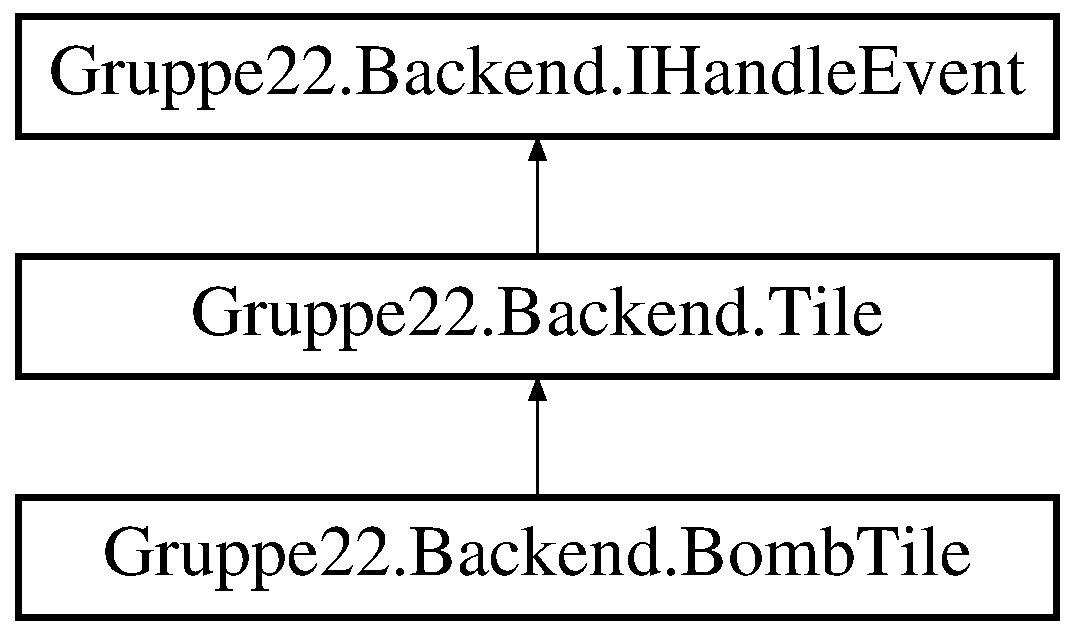
\includegraphics[height=3.000000cm]{class_gruppe22_1_1_backend_1_1_bomb_tile}
\end{center}
\end{figure}
\subsection*{Öffentliche Methoden}
\begin{DoxyCompactItemize}
\item 
\hyperlink{class_gruppe22_1_1_backend_1_1_bomb_tile_a937f553a072e251c8f5ef1e1c1f1efeb}{Bomb\-Tile} (object \hyperlink{class_gruppe22_1_1_backend_1_1_tile_abc12933c70eb3a2ebbb2fde9f45c2632}{parent})
\end{DoxyCompactItemize}
\subsection*{Weitere Geerbte Elemente}


\subsection{Beschreibung der Konstruktoren und Destruktoren}
\hypertarget{class_gruppe22_1_1_backend_1_1_bomb_tile_a937f553a072e251c8f5ef1e1c1f1efeb}{\index{Gruppe22\-::\-Backend\-::\-Bomb\-Tile@{Gruppe22\-::\-Backend\-::\-Bomb\-Tile}!Bomb\-Tile@{Bomb\-Tile}}
\index{Bomb\-Tile@{Bomb\-Tile}!Gruppe22::Backend::BombTile@{Gruppe22\-::\-Backend\-::\-Bomb\-Tile}}
\subsubsection[{Bomb\-Tile}]{\setlength{\rightskip}{0pt plus 5cm}Gruppe22.\-Backend.\-Bomb\-Tile.\-Bomb\-Tile (
\begin{DoxyParamCaption}
\item[{object}]{parent}
\end{DoxyParamCaption}
)}}\label{class_gruppe22_1_1_backend_1_1_bomb_tile_a937f553a072e251c8f5ef1e1c1f1efeb}


Die Dokumentation für diese Klasse wurde erzeugt aufgrund der Datei\-:\begin{DoxyCompactItemize}
\item 
C\-:/\-Users/beursken/\-Documents/\-Git\-Hub/gruppe22/\-Gruppe22/\-Gruppe22/\-Backend/\-Map/\hyperlink{_bomb_tile_8cs}{Bomb\-Tile.\-cs}\end{DoxyCompactItemize}

\hypertarget{class_gruppe22_1_1_client_1_1_button}{\section{Gruppe22.\-Client.\-Button Klassenreferenz}
\label{class_gruppe22_1_1_client_1_1_button}\index{Gruppe22.\-Client.\-Button@{Gruppe22.\-Client.\-Button}}
}
Klassendiagramm für Gruppe22.\-Client.\-Button\-:\begin{figure}[H]
\begin{center}
\leavevmode
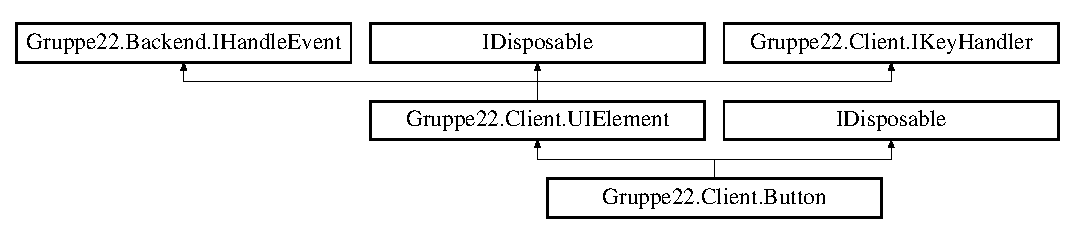
\includegraphics[height=2.692308cm]{class_gruppe22_1_1_client_1_1_button}
\end{center}
\end{figure}
\subsection*{Öffentliche Methoden}
\begin{DoxyCompactItemize}
\item 
override bool \hyperlink{class_gruppe22_1_1_client_1_1_button_aa6c6ba54e6549ee851153040fda87b0e}{On\-Mouse\-Down} (int button)
\item 
override bool \hyperlink{class_gruppe22_1_1_client_1_1_button_ad3b8e8bceadd5999af01485ed178446b}{On\-Key\-Down} (Keys k)
\begin{DoxyCompactList}\small\item\em Called whenever a key was up and is now down \end{DoxyCompactList}\item 
override void \hyperlink{class_gruppe22_1_1_client_1_1_button_a261239329db8106d9535190252571c03}{Handle\-Event} (bool downstream, \hyperlink{namespace_gruppe22_1_1_backend_ab56df91bb0bdafa1ea978e552209ce73}{Backend.\-Events} event\-I\-D, params object\mbox{[}$\,$\mbox{]} data)
\item 
override void \hyperlink{class_gruppe22_1_1_client_1_1_button_a584d2c127a7cfe8eb99c04b941aa7b68}{Show} ()
\item 
override void \hyperlink{class_gruppe22_1_1_client_1_1_button_a61fb3c2d7818fbac7131ffde637aaf3f}{Hide} ()
\item 
override void \hyperlink{class_gruppe22_1_1_client_1_1_button_a805e61d5517639ffe611f153ca19c1f3}{Draw} (Game\-Time game\-Time)
\item 
override void \hyperlink{class_gruppe22_1_1_client_1_1_button_ac2f181c74d65c94b08b86d322b22eb28}{Dispose} ()
\item 
\hyperlink{class_gruppe22_1_1_client_1_1_button_a5eb3d481c8c582938b5df89d331ba4d2}{Button} (\hyperlink{interface_gruppe22_1_1_backend_1_1_i_handle_event}{Backend.\-I\-Handle\-Event} parent, Sprite\-Batch sprite\-Batch, Content\-Manager content, Rectangle display\-Rect, string \hyperlink{namespace_gruppe22_1_1_client_ab04cc66caef13cf24be10621da9097e2afea087517c26fadd409bd4b9dc642555}{normal}, string active, string pressed, int id)
\begin{DoxyCompactList}\small\item\em Create a button using a bitmap \end{DoxyCompactList}\item 
\hyperlink{class_gruppe22_1_1_client_1_1_button_acfe21f1b4fc2cdedd3689a3c73aea3d6}{Button} (\hyperlink{interface_gruppe22_1_1_backend_1_1_i_handle_event}{Backend.\-I\-Handle\-Event} parent, Sprite\-Batch sprite\-Batch, Content\-Manager content, Rectangle display\-Rect, string label, int id, bool staydown=false)
\begin{DoxyCompactList}\small\item\em Create a button using a text label \end{DoxyCompactList}\end{DoxyCompactItemize}
\subsection*{Propertys}
\begin{DoxyCompactItemize}
\item 
override bool \hyperlink{class_gruppe22_1_1_client_1_1_button_ad3dd3b1d92337b7996d2b31dc0475e7c}{can\-Focus}\hspace{0.3cm}{\ttfamily  \mbox{[}get\mbox{]}}
\item 
bool \hyperlink{class_gruppe22_1_1_client_1_1_button_a82abfd338b674d43550df2deca15e07b}{stay\-Down}\hspace{0.3cm}{\ttfamily  \mbox{[}get, set\mbox{]}}
\begin{DoxyCompactList}\small\item\em True if the button should stay down \end{DoxyCompactList}\item 
bool \hyperlink{class_gruppe22_1_1_client_1_1_button_af4263fb04d3c59dd99f446de88155d10}{hidden}\hspace{0.3cm}{\ttfamily  \mbox{[}get, set\mbox{]}}
\end{DoxyCompactItemize}
\subsection*{Weitere Geerbte Elemente}


\subsection{Beschreibung der Konstruktoren und Destruktoren}
\hypertarget{class_gruppe22_1_1_client_1_1_button_a5eb3d481c8c582938b5df89d331ba4d2}{\index{Gruppe22\-::\-Client\-::\-Button@{Gruppe22\-::\-Client\-::\-Button}!Button@{Button}}
\index{Button@{Button}!Gruppe22::Client::Button@{Gruppe22\-::\-Client\-::\-Button}}
\subsubsection[{Button}]{\setlength{\rightskip}{0pt plus 5cm}Gruppe22.\-Client.\-Button.\-Button (
\begin{DoxyParamCaption}
\item[{{\bf Backend.\-I\-Handle\-Event}}]{parent, }
\item[{Sprite\-Batch}]{sprite\-Batch, }
\item[{Content\-Manager}]{content, }
\item[{Rectangle}]{display\-Rect, }
\item[{string}]{normal, }
\item[{string}]{active, }
\item[{string}]{pressed, }
\item[{int}]{id}
\end{DoxyParamCaption}
)}}\label{class_gruppe22_1_1_client_1_1_button_a5eb3d481c8c582938b5df89d331ba4d2}


Create a button using a bitmap 


\begin{DoxyParams}{Parameter}
{\em sprite\-Batch} & \\
\hline
{\em content} & \\
\hline
{\em display\-Rect} & \\
\hline
{\em button} & \\
\hline
{\em bpressed} & \\
\hline
{\em bmouseon} & \\
\hline
\end{DoxyParams}
\hypertarget{class_gruppe22_1_1_client_1_1_button_acfe21f1b4fc2cdedd3689a3c73aea3d6}{\index{Gruppe22\-::\-Client\-::\-Button@{Gruppe22\-::\-Client\-::\-Button}!Button@{Button}}
\index{Button@{Button}!Gruppe22::Client::Button@{Gruppe22\-::\-Client\-::\-Button}}
\subsubsection[{Button}]{\setlength{\rightskip}{0pt plus 5cm}Gruppe22.\-Client.\-Button.\-Button (
\begin{DoxyParamCaption}
\item[{{\bf Backend.\-I\-Handle\-Event}}]{parent, }
\item[{Sprite\-Batch}]{sprite\-Batch, }
\item[{Content\-Manager}]{content, }
\item[{Rectangle}]{display\-Rect, }
\item[{string}]{label, }
\item[{int}]{id, }
\item[{bool}]{staydown = {\ttfamily false}}
\end{DoxyParamCaption}
)}}\label{class_gruppe22_1_1_client_1_1_button_acfe21f1b4fc2cdedd3689a3c73aea3d6}


Create a button using a text label 


\begin{DoxyParams}{Parameter}
{\em sprite\-Batch} & \\
\hline
{\em content} & \\
\hline
{\em display\-Rect} & \\
\hline
{\em button} & \\
\hline
{\em bpressed} & \\
\hline
{\em bmouseon} & \\
\hline
\end{DoxyParams}


\subsection{Dokumentation der Elementfunktionen}
\hypertarget{class_gruppe22_1_1_client_1_1_button_ac2f181c74d65c94b08b86d322b22eb28}{\index{Gruppe22\-::\-Client\-::\-Button@{Gruppe22\-::\-Client\-::\-Button}!Dispose@{Dispose}}
\index{Dispose@{Dispose}!Gruppe22::Client::Button@{Gruppe22\-::\-Client\-::\-Button}}
\subsubsection[{Dispose}]{\setlength{\rightskip}{0pt plus 5cm}override void Gruppe22.\-Client.\-Button.\-Dispose (
\begin{DoxyParamCaption}
{}
\end{DoxyParamCaption}
)\hspace{0.3cm}{\ttfamily [virtual]}}}\label{class_gruppe22_1_1_client_1_1_button_ac2f181c74d65c94b08b86d322b22eb28}


Erneute Implementation von \hyperlink{class_gruppe22_1_1_client_1_1_u_i_element_a4dbf6405c99a1b2b45610d90e127e7fd}{Gruppe22.\-Client.\-U\-I\-Element}.

\hypertarget{class_gruppe22_1_1_client_1_1_button_a805e61d5517639ffe611f153ca19c1f3}{\index{Gruppe22\-::\-Client\-::\-Button@{Gruppe22\-::\-Client\-::\-Button}!Draw@{Draw}}
\index{Draw@{Draw}!Gruppe22::Client::Button@{Gruppe22\-::\-Client\-::\-Button}}
\subsubsection[{Draw}]{\setlength{\rightskip}{0pt plus 5cm}override void Gruppe22.\-Client.\-Button.\-Draw (
\begin{DoxyParamCaption}
\item[{Game\-Time}]{game\-Time}
\end{DoxyParamCaption}
)\hspace{0.3cm}{\ttfamily [virtual]}}}\label{class_gruppe22_1_1_client_1_1_button_a805e61d5517639ffe611f153ca19c1f3}





\begin{DoxyParams}{Parameter}
{\em sprite\-Batch} & \\
\hline
\end{DoxyParams}


Erneute Implementation von \hyperlink{class_gruppe22_1_1_client_1_1_u_i_element_ae68afcbd1db3540052d6b399022e56e7}{Gruppe22.\-Client.\-U\-I\-Element}.

\hypertarget{class_gruppe22_1_1_client_1_1_button_a261239329db8106d9535190252571c03}{\index{Gruppe22\-::\-Client\-::\-Button@{Gruppe22\-::\-Client\-::\-Button}!Handle\-Event@{Handle\-Event}}
\index{Handle\-Event@{Handle\-Event}!Gruppe22::Client::Button@{Gruppe22\-::\-Client\-::\-Button}}
\subsubsection[{Handle\-Event}]{\setlength{\rightskip}{0pt plus 5cm}override void Gruppe22.\-Client.\-Button.\-Handle\-Event (
\begin{DoxyParamCaption}
\item[{bool}]{downstream, }
\item[{{\bf Backend.\-Events}}]{event\-I\-D, }
\item[{params object\mbox{[}$\,$\mbox{]}}]{data}
\end{DoxyParamCaption}
)\hspace{0.3cm}{\ttfamily [virtual]}}}\label{class_gruppe22_1_1_client_1_1_button_a261239329db8106d9535190252571c03}


Erneute Implementation von \hyperlink{class_gruppe22_1_1_client_1_1_u_i_element_ad06a1ce6c1705a1c7aa91756f368a517}{Gruppe22.\-Client.\-U\-I\-Element}.

\hypertarget{class_gruppe22_1_1_client_1_1_button_a61fb3c2d7818fbac7131ffde637aaf3f}{\index{Gruppe22\-::\-Client\-::\-Button@{Gruppe22\-::\-Client\-::\-Button}!Hide@{Hide}}
\index{Hide@{Hide}!Gruppe22::Client::Button@{Gruppe22\-::\-Client\-::\-Button}}
\subsubsection[{Hide}]{\setlength{\rightskip}{0pt plus 5cm}override void Gruppe22.\-Client.\-Button.\-Hide (
\begin{DoxyParamCaption}
{}
\end{DoxyParamCaption}
)\hspace{0.3cm}{\ttfamily [virtual]}}}\label{class_gruppe22_1_1_client_1_1_button_a61fb3c2d7818fbac7131ffde637aaf3f}


Erneute Implementation von \hyperlink{class_gruppe22_1_1_client_1_1_u_i_element_a0758d4427656b0109fc2ded57e83c0a9}{Gruppe22.\-Client.\-U\-I\-Element}.

\hypertarget{class_gruppe22_1_1_client_1_1_button_ad3b8e8bceadd5999af01485ed178446b}{\index{Gruppe22\-::\-Client\-::\-Button@{Gruppe22\-::\-Client\-::\-Button}!On\-Key\-Down@{On\-Key\-Down}}
\index{On\-Key\-Down@{On\-Key\-Down}!Gruppe22::Client::Button@{Gruppe22\-::\-Client\-::\-Button}}
\subsubsection[{On\-Key\-Down}]{\setlength{\rightskip}{0pt plus 5cm}override bool Gruppe22.\-Client.\-Button.\-On\-Key\-Down (
\begin{DoxyParamCaption}
\item[{Keys}]{k}
\end{DoxyParamCaption}
)\hspace{0.3cm}{\ttfamily [virtual]}}}\label{class_gruppe22_1_1_client_1_1_button_ad3b8e8bceadd5999af01485ed178446b}


Called whenever a key was up and is now down 


\begin{DoxyParams}{Parameter}
{\em k} & The key which was pressed\\
\hline
\end{DoxyParams}


Erneute Implementation von \hyperlink{class_gruppe22_1_1_client_1_1_u_i_element_a0f9957f48ecb697ff5ae1ac3f0873064}{Gruppe22.\-Client.\-U\-I\-Element}.

\hypertarget{class_gruppe22_1_1_client_1_1_button_aa6c6ba54e6549ee851153040fda87b0e}{\index{Gruppe22\-::\-Client\-::\-Button@{Gruppe22\-::\-Client\-::\-Button}!On\-Mouse\-Down@{On\-Mouse\-Down}}
\index{On\-Mouse\-Down@{On\-Mouse\-Down}!Gruppe22::Client::Button@{Gruppe22\-::\-Client\-::\-Button}}
\subsubsection[{On\-Mouse\-Down}]{\setlength{\rightskip}{0pt plus 5cm}override bool Gruppe22.\-Client.\-Button.\-On\-Mouse\-Down (
\begin{DoxyParamCaption}
\item[{int}]{button}
\end{DoxyParamCaption}
)\hspace{0.3cm}{\ttfamily [virtual]}}}\label{class_gruppe22_1_1_client_1_1_button_aa6c6ba54e6549ee851153040fda87b0e}





\begin{DoxyParams}{Parameter}
{\em game\-Time} & \\
\hline
\end{DoxyParams}


Erneute Implementation von \hyperlink{class_gruppe22_1_1_client_1_1_u_i_element_a0530df2286336160b8b39c74ba380a44}{Gruppe22.\-Client.\-U\-I\-Element}.

\hypertarget{class_gruppe22_1_1_client_1_1_button_a584d2c127a7cfe8eb99c04b941aa7b68}{\index{Gruppe22\-::\-Client\-::\-Button@{Gruppe22\-::\-Client\-::\-Button}!Show@{Show}}
\index{Show@{Show}!Gruppe22::Client::Button@{Gruppe22\-::\-Client\-::\-Button}}
\subsubsection[{Show}]{\setlength{\rightskip}{0pt plus 5cm}override void Gruppe22.\-Client.\-Button.\-Show (
\begin{DoxyParamCaption}
{}
\end{DoxyParamCaption}
)\hspace{0.3cm}{\ttfamily [virtual]}}}\label{class_gruppe22_1_1_client_1_1_button_a584d2c127a7cfe8eb99c04b941aa7b68}


Erneute Implementation von \hyperlink{class_gruppe22_1_1_client_1_1_u_i_element_a7d3595683a3f3e3a18788301e432204a}{Gruppe22.\-Client.\-U\-I\-Element}.



\subsection{Dokumentation der Propertys}
\hypertarget{class_gruppe22_1_1_client_1_1_button_ad3dd3b1d92337b7996d2b31dc0475e7c}{\index{Gruppe22\-::\-Client\-::\-Button@{Gruppe22\-::\-Client\-::\-Button}!can\-Focus@{can\-Focus}}
\index{can\-Focus@{can\-Focus}!Gruppe22::Client::Button@{Gruppe22\-::\-Client\-::\-Button}}
\subsubsection[{can\-Focus}]{\setlength{\rightskip}{0pt plus 5cm}override bool Gruppe22.\-Client.\-Button.\-can\-Focus\hspace{0.3cm}{\ttfamily [get]}}}\label{class_gruppe22_1_1_client_1_1_button_ad3dd3b1d92337b7996d2b31dc0475e7c}
\hypertarget{class_gruppe22_1_1_client_1_1_button_af4263fb04d3c59dd99f446de88155d10}{\index{Gruppe22\-::\-Client\-::\-Button@{Gruppe22\-::\-Client\-::\-Button}!hidden@{hidden}}
\index{hidden@{hidden}!Gruppe22::Client::Button@{Gruppe22\-::\-Client\-::\-Button}}
\subsubsection[{hidden}]{\setlength{\rightskip}{0pt plus 5cm}bool Gruppe22.\-Client.\-Button.\-hidden\hspace{0.3cm}{\ttfamily [get]}, {\ttfamily [set]}}}\label{class_gruppe22_1_1_client_1_1_button_af4263fb04d3c59dd99f446de88155d10}
\hypertarget{class_gruppe22_1_1_client_1_1_button_a82abfd338b674d43550df2deca15e07b}{\index{Gruppe22\-::\-Client\-::\-Button@{Gruppe22\-::\-Client\-::\-Button}!stay\-Down@{stay\-Down}}
\index{stay\-Down@{stay\-Down}!Gruppe22::Client::Button@{Gruppe22\-::\-Client\-::\-Button}}
\subsubsection[{stay\-Down}]{\setlength{\rightskip}{0pt plus 5cm}bool Gruppe22.\-Client.\-Button.\-stay\-Down\hspace{0.3cm}{\ttfamily [get]}, {\ttfamily [set]}}}\label{class_gruppe22_1_1_client_1_1_button_a82abfd338b674d43550df2deca15e07b}


True if the button should stay down 



Die Dokumentation für diese Klasse wurde erzeugt aufgrund der Datei\-:\begin{DoxyCompactItemize}
\item 
C\-:/\-Users/beursken/\-Documents/\-Git\-Hub/gruppe22/\-Gruppe22/\-Gruppe22/\-Client/\-U\-I/\hyperlink{_button_8cs}{Button.\-cs}\end{DoxyCompactItemize}

\hypertarget{class_gruppe22_1_1_client_1_1_camera}{\section{Gruppe22.\-Client.\-Camera Klassenreferenz}
\label{class_gruppe22_1_1_client_1_1_camera}\index{Gruppe22.\-Client.\-Camera@{Gruppe22.\-Client.\-Camera}}
}
\subsection*{Öffentliche Methoden}
\begin{DoxyCompactItemize}
\item 
void \hyperlink{class_gruppe22_1_1_client_1_1_camera_abf680aa4aded267b32bfef475b7bb501}{Move} (Vector2 amount)
\begin{DoxyCompactList}\small\item\em Move the \hyperlink{class_gruppe22_1_1_client_1_1_camera}{Camera} by a specified amount vertically and horizontally \end{DoxyCompactList}\item 
void \hyperlink{class_gruppe22_1_1_client_1_1_camera_a824e5423328b7b27da3bf7d81635eb7a}{Reset\-Center} (Vector2 center)
\item 
\hyperlink{class_gruppe22_1_1_client_1_1_camera_a2c0251a91cfa20eebd252632d2805717}{Camera} (Vector2 center)
\end{DoxyCompactItemize}
\subsection*{Propertys}
\begin{DoxyCompactItemize}
\item 
float \hyperlink{class_gruppe22_1_1_client_1_1_camera_aa80119f5c2ba8766d65b2797ded61964}{zoom}\hspace{0.3cm}{\ttfamily  \mbox{[}get, set\mbox{]}}
\begin{DoxyCompactList}\small\item\em Get or set the camera's zoom level \end{DoxyCompactList}\item 
float \hyperlink{class_gruppe22_1_1_client_1_1_camera_af79ef77a21b4c349e32e4fd07c1a618b}{rotate}\hspace{0.3cm}{\ttfamily  \mbox{[}get, set\mbox{]}}
\item 
Vector2 \hyperlink{class_gruppe22_1_1_client_1_1_camera_a1e2d1783c015ab1a8de5f7a4e6457815}{position}\hspace{0.3cm}{\ttfamily  \mbox{[}get, set\mbox{]}}
\begin{DoxyCompactList}\small\item\em Get or set the camera's position \end{DoxyCompactList}\item 
Matrix \hyperlink{class_gruppe22_1_1_client_1_1_camera_af30d0c300b6a206f1552b4cfd7befeed}{matrix}\hspace{0.3cm}{\ttfamily  \mbox{[}get\mbox{]}}
\begin{DoxyCompactList}\small\item\em Get a transformation matrix moving a camera to the specified position and zoom level \end{DoxyCompactList}\end{DoxyCompactItemize}


\subsection{Beschreibung der Konstruktoren und Destruktoren}
\hypertarget{class_gruppe22_1_1_client_1_1_camera_a2c0251a91cfa20eebd252632d2805717}{\index{Gruppe22\-::\-Client\-::\-Camera@{Gruppe22\-::\-Client\-::\-Camera}!Camera@{Camera}}
\index{Camera@{Camera}!Gruppe22::Client::Camera@{Gruppe22\-::\-Client\-::\-Camera}}
\subsubsection[{Camera}]{\setlength{\rightskip}{0pt plus 5cm}Gruppe22.\-Client.\-Camera.\-Camera (
\begin{DoxyParamCaption}
\item[{Vector2}]{center}
\end{DoxyParamCaption}
)}}\label{class_gruppe22_1_1_client_1_1_camera_a2c0251a91cfa20eebd252632d2805717}


\subsection{Dokumentation der Elementfunktionen}
\hypertarget{class_gruppe22_1_1_client_1_1_camera_abf680aa4aded267b32bfef475b7bb501}{\index{Gruppe22\-::\-Client\-::\-Camera@{Gruppe22\-::\-Client\-::\-Camera}!Move@{Move}}
\index{Move@{Move}!Gruppe22::Client::Camera@{Gruppe22\-::\-Client\-::\-Camera}}
\subsubsection[{Move}]{\setlength{\rightskip}{0pt plus 5cm}void Gruppe22.\-Client.\-Camera.\-Move (
\begin{DoxyParamCaption}
\item[{Vector2}]{amount}
\end{DoxyParamCaption}
)}}\label{class_gruppe22_1_1_client_1_1_camera_abf680aa4aded267b32bfef475b7bb501}


Move the \hyperlink{class_gruppe22_1_1_client_1_1_camera}{Camera} by a specified amount vertically and horizontally 


\begin{DoxyParams}{Parameter}
{\em amount} & The number of pixels to move the camera\\
\hline
\end{DoxyParams}
\hypertarget{class_gruppe22_1_1_client_1_1_camera_a824e5423328b7b27da3bf7d81635eb7a}{\index{Gruppe22\-::\-Client\-::\-Camera@{Gruppe22\-::\-Client\-::\-Camera}!Reset\-Center@{Reset\-Center}}
\index{Reset\-Center@{Reset\-Center}!Gruppe22::Client::Camera@{Gruppe22\-::\-Client\-::\-Camera}}
\subsubsection[{Reset\-Center}]{\setlength{\rightskip}{0pt plus 5cm}void Gruppe22.\-Client.\-Camera.\-Reset\-Center (
\begin{DoxyParamCaption}
\item[{Vector2}]{center}
\end{DoxyParamCaption}
)}}\label{class_gruppe22_1_1_client_1_1_camera_a824e5423328b7b27da3bf7d81635eb7a}


\subsection{Dokumentation der Propertys}
\hypertarget{class_gruppe22_1_1_client_1_1_camera_af30d0c300b6a206f1552b4cfd7befeed}{\index{Gruppe22\-::\-Client\-::\-Camera@{Gruppe22\-::\-Client\-::\-Camera}!matrix@{matrix}}
\index{matrix@{matrix}!Gruppe22::Client::Camera@{Gruppe22\-::\-Client\-::\-Camera}}
\subsubsection[{matrix}]{\setlength{\rightskip}{0pt plus 5cm}Matrix Gruppe22.\-Client.\-Camera.\-matrix\hspace{0.3cm}{\ttfamily [get]}}}\label{class_gruppe22_1_1_client_1_1_camera_af30d0c300b6a206f1552b4cfd7befeed}


Get a transformation matrix moving a camera to the specified position and zoom level 


\begin{DoxyParams}{Parameter}
{\em \-\_\-graphics} & The device to use for calculating the matrix\\
\hline
\end{DoxyParams}
\begin{DoxyReturn}{Rückgabe}

\end{DoxyReturn}
\hypertarget{class_gruppe22_1_1_client_1_1_camera_a1e2d1783c015ab1a8de5f7a4e6457815}{\index{Gruppe22\-::\-Client\-::\-Camera@{Gruppe22\-::\-Client\-::\-Camera}!position@{position}}
\index{position@{position}!Gruppe22::Client::Camera@{Gruppe22\-::\-Client\-::\-Camera}}
\subsubsection[{position}]{\setlength{\rightskip}{0pt plus 5cm}Vector2 Gruppe22.\-Client.\-Camera.\-position\hspace{0.3cm}{\ttfamily [get]}, {\ttfamily [set]}}}\label{class_gruppe22_1_1_client_1_1_camera_a1e2d1783c015ab1a8de5f7a4e6457815}


Get or set the camera's position 

\hypertarget{class_gruppe22_1_1_client_1_1_camera_af79ef77a21b4c349e32e4fd07c1a618b}{\index{Gruppe22\-::\-Client\-::\-Camera@{Gruppe22\-::\-Client\-::\-Camera}!rotate@{rotate}}
\index{rotate@{rotate}!Gruppe22::Client::Camera@{Gruppe22\-::\-Client\-::\-Camera}}
\subsubsection[{rotate}]{\setlength{\rightskip}{0pt plus 5cm}float Gruppe22.\-Client.\-Camera.\-rotate\hspace{0.3cm}{\ttfamily [get]}, {\ttfamily [set]}}}\label{class_gruppe22_1_1_client_1_1_camera_af79ef77a21b4c349e32e4fd07c1a618b}
\hypertarget{class_gruppe22_1_1_client_1_1_camera_aa80119f5c2ba8766d65b2797ded61964}{\index{Gruppe22\-::\-Client\-::\-Camera@{Gruppe22\-::\-Client\-::\-Camera}!zoom@{zoom}}
\index{zoom@{zoom}!Gruppe22::Client::Camera@{Gruppe22\-::\-Client\-::\-Camera}}
\subsubsection[{zoom}]{\setlength{\rightskip}{0pt plus 5cm}float Gruppe22.\-Client.\-Camera.\-zoom\hspace{0.3cm}{\ttfamily [get]}, {\ttfamily [set]}}}\label{class_gruppe22_1_1_client_1_1_camera_aa80119f5c2ba8766d65b2797ded61964}


Get or set the camera's zoom level 



Die Dokumentation für diese Klasse wurde erzeugt aufgrund der Datei\-:\begin{DoxyCompactItemize}
\item 
C\-:/\-Users/beursken/\-Documents/\-Git\-Hub/gruppe22/\-Gruppe22/\-Gruppe22/\-Client/\-Map/\hyperlink{_camera_8cs}{Camera.\-cs}\end{DoxyCompactItemize}

\hypertarget{class_gruppe22_1_1_client_1_1_character_window}{\section{Gruppe22.\-Client.\-Character\-Window Klassenreferenz}
\label{class_gruppe22_1_1_client_1_1_character_window}\index{Gruppe22.\-Client.\-Character\-Window@{Gruppe22.\-Client.\-Character\-Window}}
}
Klassendiagramm für Gruppe22.\-Client.\-Character\-Window\-:\begin{figure}[H]
\begin{center}
\leavevmode
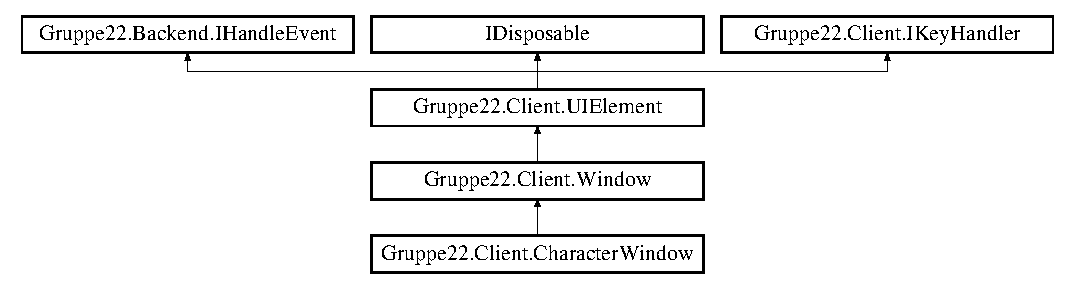
\includegraphics[height=3.440860cm]{class_gruppe22_1_1_client_1_1_character_window}
\end{center}
\end{figure}
\subsection*{Öffentliche Methoden}
\begin{DoxyCompactItemize}
\item 
override void \hyperlink{class_gruppe22_1_1_client_1_1_character_window_a048ae6a552fbaa709f33c19730d593f3}{Handle\-Event} (bool Down\-Stream, \hyperlink{namespace_gruppe22_1_1_backend_ab56df91bb0bdafa1ea978e552209ce73}{Backend.\-Events} event\-I\-D, params object\mbox{[}$\,$\mbox{]} data)
\item 
override bool \hyperlink{class_gruppe22_1_1_client_1_1_character_window_abb07535d47bf7bcecfc92045c9a91116}{On\-Mouse\-Down} (int button)
\begin{DoxyCompactList}\small\item\em Called when a mouse button changes from up to down \end{DoxyCompactList}\item 
override void \hyperlink{class_gruppe22_1_1_client_1_1_character_window_a9cd2befa924c9fdf68a0428d9ed1746e}{Draw} (Game\-Time game\-Time)
\item 
\hyperlink{class_gruppe22_1_1_client_1_1_character_window_abc793603a863ec208d9e86ddb8514525}{Character\-Window} (\hyperlink{interface_gruppe22_1_1_backend_1_1_i_handle_event}{Backend.\-I\-Handle\-Event} parent, Sprite\-Batch sprite\-Batch, Content\-Manager content, Rectangle display\-Rect, \hyperlink{class_gruppe22_1_1_backend_1_1_actor}{Backend.\-Actor} actor)
\begin{DoxyCompactList}\small\item\em Constructor \end{DoxyCompactList}\end{DoxyCompactItemize}
\subsection*{Geschützte Attribute}
\begin{DoxyCompactItemize}
\item 
Sprite\-Font \hyperlink{class_gruppe22_1_1_client_1_1_character_window_a3f8069e41adb888c44baf666c251a2a8}{\-\_\-font} = null
\end{DoxyCompactItemize}
\subsection*{Propertys}
\begin{DoxyCompactItemize}
\item 
uint \hyperlink{class_gruppe22_1_1_client_1_1_character_window_ac8d2bb9506d4bd08d868670e934538b6}{page}\hspace{0.3cm}{\ttfamily  \mbox{[}get, set\mbox{]}}
\end{DoxyCompactItemize}


\subsection{Beschreibung der Konstruktoren und Destruktoren}
\hypertarget{class_gruppe22_1_1_client_1_1_character_window_abc793603a863ec208d9e86ddb8514525}{\index{Gruppe22\-::\-Client\-::\-Character\-Window@{Gruppe22\-::\-Client\-::\-Character\-Window}!Character\-Window@{Character\-Window}}
\index{Character\-Window@{Character\-Window}!Gruppe22::Client::CharacterWindow@{Gruppe22\-::\-Client\-::\-Character\-Window}}
\subsubsection[{Character\-Window}]{\setlength{\rightskip}{0pt plus 5cm}Gruppe22.\-Client.\-Character\-Window.\-Character\-Window (
\begin{DoxyParamCaption}
\item[{{\bf Backend.\-I\-Handle\-Event}}]{parent, }
\item[{Sprite\-Batch}]{sprite\-Batch, }
\item[{Content\-Manager}]{content, }
\item[{Rectangle}]{display\-Rect, }
\item[{{\bf Backend.\-Actor}}]{actor}
\end{DoxyParamCaption}
)}}\label{class_gruppe22_1_1_client_1_1_character_window_abc793603a863ec208d9e86ddb8514525}


Constructor 



\subsection{Dokumentation der Elementfunktionen}
\hypertarget{class_gruppe22_1_1_client_1_1_character_window_a9cd2befa924c9fdf68a0428d9ed1746e}{\index{Gruppe22\-::\-Client\-::\-Character\-Window@{Gruppe22\-::\-Client\-::\-Character\-Window}!Draw@{Draw}}
\index{Draw@{Draw}!Gruppe22::Client::CharacterWindow@{Gruppe22\-::\-Client\-::\-Character\-Window}}
\subsubsection[{Draw}]{\setlength{\rightskip}{0pt plus 5cm}override void Gruppe22.\-Client.\-Character\-Window.\-Draw (
\begin{DoxyParamCaption}
\item[{Game\-Time}]{game\-Time}
\end{DoxyParamCaption}
)\hspace{0.3cm}{\ttfamily [virtual]}}}\label{class_gruppe22_1_1_client_1_1_character_window_a9cd2befa924c9fdf68a0428d9ed1746e}





\begin{DoxyParams}{Parameter}
{\em game\-Time} & \\
\hline
\end{DoxyParams}


Erneute Implementation von \hyperlink{class_gruppe22_1_1_client_1_1_u_i_element_ae68afcbd1db3540052d6b399022e56e7}{Gruppe22.\-Client.\-U\-I\-Element}.

\hypertarget{class_gruppe22_1_1_client_1_1_character_window_a048ae6a552fbaa709f33c19730d593f3}{\index{Gruppe22\-::\-Client\-::\-Character\-Window@{Gruppe22\-::\-Client\-::\-Character\-Window}!Handle\-Event@{Handle\-Event}}
\index{Handle\-Event@{Handle\-Event}!Gruppe22::Client::CharacterWindow@{Gruppe22\-::\-Client\-::\-Character\-Window}}
\subsubsection[{Handle\-Event}]{\setlength{\rightskip}{0pt plus 5cm}override void Gruppe22.\-Client.\-Character\-Window.\-Handle\-Event (
\begin{DoxyParamCaption}
\item[{bool}]{Down\-Stream, }
\item[{{\bf Backend.\-Events}}]{event\-I\-D, }
\item[{params object\mbox{[}$\,$\mbox{]}}]{data}
\end{DoxyParamCaption}
)\hspace{0.3cm}{\ttfamily [virtual]}}}\label{class_gruppe22_1_1_client_1_1_character_window_a048ae6a552fbaa709f33c19730d593f3}


Erneute Implementation von \hyperlink{class_gruppe22_1_1_client_1_1_u_i_element_ad06a1ce6c1705a1c7aa91756f368a517}{Gruppe22.\-Client.\-U\-I\-Element}.

\hypertarget{class_gruppe22_1_1_client_1_1_character_window_abb07535d47bf7bcecfc92045c9a91116}{\index{Gruppe22\-::\-Client\-::\-Character\-Window@{Gruppe22\-::\-Client\-::\-Character\-Window}!On\-Mouse\-Down@{On\-Mouse\-Down}}
\index{On\-Mouse\-Down@{On\-Mouse\-Down}!Gruppe22::Client::CharacterWindow@{Gruppe22\-::\-Client\-::\-Character\-Window}}
\subsubsection[{On\-Mouse\-Down}]{\setlength{\rightskip}{0pt plus 5cm}override bool Gruppe22.\-Client.\-Character\-Window.\-On\-Mouse\-Down (
\begin{DoxyParamCaption}
\item[{int}]{button}
\end{DoxyParamCaption}
)\hspace{0.3cm}{\ttfamily [virtual]}}}\label{class_gruppe22_1_1_client_1_1_character_window_abb07535d47bf7bcecfc92045c9a91116}


Called when a mouse button changes from up to down 


\begin{DoxyParams}{Parameter}
{\em button} & Left \hyperlink{class_gruppe22_1_1_client_1_1_button}{Button}=1, Middle \hyperlink{class_gruppe22_1_1_client_1_1_button}{Button}=2, Right \hyperlink{class_gruppe22_1_1_client_1_1_button}{Button}=3\\
\hline
\end{DoxyParams}


Erneute Implementation von \hyperlink{class_gruppe22_1_1_client_1_1_u_i_element_a0530df2286336160b8b39c74ba380a44}{Gruppe22.\-Client.\-U\-I\-Element}.



\subsection{Dokumentation der Datenelemente}
\hypertarget{class_gruppe22_1_1_client_1_1_character_window_a3f8069e41adb888c44baf666c251a2a8}{\index{Gruppe22\-::\-Client\-::\-Character\-Window@{Gruppe22\-::\-Client\-::\-Character\-Window}!\-\_\-font@{\-\_\-font}}
\index{\-\_\-font@{\-\_\-font}!Gruppe22::Client::CharacterWindow@{Gruppe22\-::\-Client\-::\-Character\-Window}}
\subsubsection[{\-\_\-font}]{\setlength{\rightskip}{0pt plus 5cm}Sprite\-Font Gruppe22.\-Client.\-Character\-Window.\-\_\-font = null\hspace{0.3cm}{\ttfamily [protected]}}}\label{class_gruppe22_1_1_client_1_1_character_window_a3f8069e41adb888c44baf666c251a2a8}


\subsection{Dokumentation der Propertys}
\hypertarget{class_gruppe22_1_1_client_1_1_character_window_ac8d2bb9506d4bd08d868670e934538b6}{\index{Gruppe22\-::\-Client\-::\-Character\-Window@{Gruppe22\-::\-Client\-::\-Character\-Window}!page@{page}}
\index{page@{page}!Gruppe22::Client::CharacterWindow@{Gruppe22\-::\-Client\-::\-Character\-Window}}
\subsubsection[{page}]{\setlength{\rightskip}{0pt plus 5cm}uint Gruppe22.\-Client.\-Character\-Window.\-page\hspace{0.3cm}{\ttfamily [get]}, {\ttfamily [set]}}}\label{class_gruppe22_1_1_client_1_1_character_window_ac8d2bb9506d4bd08d868670e934538b6}


Die Dokumentation für diese Klasse wurde erzeugt aufgrund der Datei\-:\begin{DoxyCompactItemize}
\item 
C\-:/\-Users/beursken/\-Documents/\-Git\-Hub/gruppe22/\-Gruppe22/\-Gruppe22/\-Client/\-U\-I/\hyperlink{_character_window_8cs}{Character\-Window.\-cs}\end{DoxyCompactItemize}

\hypertarget{class_gruppe22_1_1_client_1_1_chat}{\section{Gruppe22.\-Client.\-Chat Klassenreferenz}
\label{class_gruppe22_1_1_client_1_1_chat}\index{Gruppe22.\-Client.\-Chat@{Gruppe22.\-Client.\-Chat}}
}
Klassendiagramm für Gruppe22.\-Client.\-Chat\-:\begin{figure}[H]
\begin{center}
\leavevmode
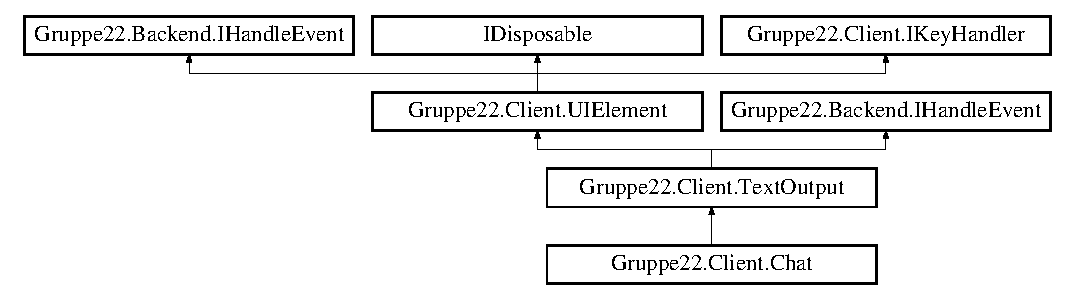
\includegraphics[height=3.589744cm]{class_gruppe22_1_1_client_1_1_chat}
\end{center}
\end{figure}
\subsection*{Öffentliche Methoden}
\begin{DoxyCompactItemize}
\item 
override void \hyperlink{class_gruppe22_1_1_client_1_1_chat_a4caef8eac20c6ac2094ca85de9ce2404}{Add\-Line} (string text, object color=null)
\begin{DoxyCompactList}\small\item\em Add a line of text to output (requires implementation in children \end{DoxyCompactList}\item 
override void \hyperlink{class_gruppe22_1_1_client_1_1_chat_a505f59e3352f8170506adf261b2c5091}{Update} (Game\-Time game\-Time)
\item 
override void \hyperlink{class_gruppe22_1_1_client_1_1_chat_a38eabd876d056f309733920d48529b8d}{Draw} (Game\-Time game\-Time)
\item 
override bool \hyperlink{class_gruppe22_1_1_client_1_1_chat_a262b6a8fbff282b5dc6a4608aec1bee7}{On\-Key\-Down} (Microsoft.\-Xna.\-Framework.\-Input.\-Keys k)
\item 
override bool \hyperlink{class_gruppe22_1_1_client_1_1_chat_aa5fdd87b71df060f018268a07dce5ed8}{On\-Mouse\-Down} (int button)
\begin{DoxyCompactList}\small\item\em Called when a mouse button changes from up to down \end{DoxyCompactList}\item 
override void \hyperlink{class_gruppe22_1_1_client_1_1_chat_a82d35f852f996141331bda83b17876ff}{Handle\-Event} (bool Down\-Stream, \hyperlink{namespace_gruppe22_1_1_backend_ab56df91bb0bdafa1ea978e552209ce73}{Backend.\-Events} event\-I\-D, params object\mbox{[}$\,$\mbox{]} data)
\item 
\hyperlink{class_gruppe22_1_1_client_1_1_chat_a826ffa624399278465040c080217495e}{Chat} (\hyperlink{interface_gruppe22_1_1_backend_1_1_i_handle_event}{Backend.\-I\-Handle\-Event} parent, Sprite\-Batch sprite\-Batch, Content\-Manager content, Rectangle display\-Rect, bool has\-Border=true, bool center=false)
\end{DoxyCompactItemize}
\subsection*{Propertys}
\begin{DoxyCompactItemize}
\item 
override bool \hyperlink{class_gruppe22_1_1_client_1_1_chat_a0d034dac8f50fa69a98c3e4a6c574150}{focus}\hspace{0.3cm}{\ttfamily  \mbox{[}get, set\mbox{]}}
\end{DoxyCompactItemize}
\subsection*{Weitere Geerbte Elemente}


\subsection{Beschreibung der Konstruktoren und Destruktoren}
\hypertarget{class_gruppe22_1_1_client_1_1_chat_a826ffa624399278465040c080217495e}{\index{Gruppe22\-::\-Client\-::\-Chat@{Gruppe22\-::\-Client\-::\-Chat}!Chat@{Chat}}
\index{Chat@{Chat}!Gruppe22::Client::Chat@{Gruppe22\-::\-Client\-::\-Chat}}
\subsubsection[{Chat}]{\setlength{\rightskip}{0pt plus 5cm}Gruppe22.\-Client.\-Chat.\-Chat (
\begin{DoxyParamCaption}
\item[{{\bf Backend.\-I\-Handle\-Event}}]{parent, }
\item[{Sprite\-Batch}]{sprite\-Batch, }
\item[{Content\-Manager}]{content, }
\item[{Rectangle}]{display\-Rect, }
\item[{bool}]{has\-Border = {\ttfamily true}, }
\item[{bool}]{center = {\ttfamily false}}
\end{DoxyParamCaption}
)}}\label{class_gruppe22_1_1_client_1_1_chat_a826ffa624399278465040c080217495e}


\subsection{Dokumentation der Elementfunktionen}
\hypertarget{class_gruppe22_1_1_client_1_1_chat_a4caef8eac20c6ac2094ca85de9ce2404}{\index{Gruppe22\-::\-Client\-::\-Chat@{Gruppe22\-::\-Client\-::\-Chat}!Add\-Line@{Add\-Line}}
\index{Add\-Line@{Add\-Line}!Gruppe22::Client::Chat@{Gruppe22\-::\-Client\-::\-Chat}}
\subsubsection[{Add\-Line}]{\setlength{\rightskip}{0pt plus 5cm}override void Gruppe22.\-Client.\-Chat.\-Add\-Line (
\begin{DoxyParamCaption}
\item[{string}]{text, }
\item[{object}]{color = {\ttfamily null}}
\end{DoxyParamCaption}
)\hspace{0.3cm}{\ttfamily [virtual]}}}\label{class_gruppe22_1_1_client_1_1_chat_a4caef8eac20c6ac2094ca85de9ce2404}


Add a line of text to output (requires implementation in children 


\begin{DoxyParams}{Parameter}
{\em text} & \\
\hline
{\em color} & \\
\hline
\end{DoxyParams}


Erneute Implementation von \hyperlink{class_gruppe22_1_1_client_1_1_text_output_a1350976d5c45cef2d5227b5c4e097896}{Gruppe22.\-Client.\-Text\-Output}.

\hypertarget{class_gruppe22_1_1_client_1_1_chat_a38eabd876d056f309733920d48529b8d}{\index{Gruppe22\-::\-Client\-::\-Chat@{Gruppe22\-::\-Client\-::\-Chat}!Draw@{Draw}}
\index{Draw@{Draw}!Gruppe22::Client::Chat@{Gruppe22\-::\-Client\-::\-Chat}}
\subsubsection[{Draw}]{\setlength{\rightskip}{0pt plus 5cm}override void Gruppe22.\-Client.\-Chat.\-Draw (
\begin{DoxyParamCaption}
\item[{Game\-Time}]{game\-Time}
\end{DoxyParamCaption}
)\hspace{0.3cm}{\ttfamily [virtual]}}}\label{class_gruppe22_1_1_client_1_1_chat_a38eabd876d056f309733920d48529b8d}





\begin{DoxyParams}{Parameter}
{\em game\-Time} & \\
\hline
\end{DoxyParams}


Erneute Implementation von \hyperlink{class_gruppe22_1_1_client_1_1_u_i_element_ae68afcbd1db3540052d6b399022e56e7}{Gruppe22.\-Client.\-U\-I\-Element}.

\hypertarget{class_gruppe22_1_1_client_1_1_chat_a82d35f852f996141331bda83b17876ff}{\index{Gruppe22\-::\-Client\-::\-Chat@{Gruppe22\-::\-Client\-::\-Chat}!Handle\-Event@{Handle\-Event}}
\index{Handle\-Event@{Handle\-Event}!Gruppe22::Client::Chat@{Gruppe22\-::\-Client\-::\-Chat}}
\subsubsection[{Handle\-Event}]{\setlength{\rightskip}{0pt plus 5cm}override void Gruppe22.\-Client.\-Chat.\-Handle\-Event (
\begin{DoxyParamCaption}
\item[{bool}]{Down\-Stream, }
\item[{{\bf Backend.\-Events}}]{event\-I\-D, }
\item[{params object\mbox{[}$\,$\mbox{]}}]{data}
\end{DoxyParamCaption}
)\hspace{0.3cm}{\ttfamily [virtual]}}}\label{class_gruppe22_1_1_client_1_1_chat_a82d35f852f996141331bda83b17876ff}


Erneute Implementation von \hyperlink{class_gruppe22_1_1_client_1_1_u_i_element_ad06a1ce6c1705a1c7aa91756f368a517}{Gruppe22.\-Client.\-U\-I\-Element}.

\hypertarget{class_gruppe22_1_1_client_1_1_chat_a262b6a8fbff282b5dc6a4608aec1bee7}{\index{Gruppe22\-::\-Client\-::\-Chat@{Gruppe22\-::\-Client\-::\-Chat}!On\-Key\-Down@{On\-Key\-Down}}
\index{On\-Key\-Down@{On\-Key\-Down}!Gruppe22::Client::Chat@{Gruppe22\-::\-Client\-::\-Chat}}
\subsubsection[{On\-Key\-Down}]{\setlength{\rightskip}{0pt plus 5cm}override bool Gruppe22.\-Client.\-Chat.\-On\-Key\-Down (
\begin{DoxyParamCaption}
\item[{Microsoft.\-Xna.\-Framework.\-Input.\-Keys}]{k}
\end{DoxyParamCaption}
)}}\label{class_gruppe22_1_1_client_1_1_chat_a262b6a8fbff282b5dc6a4608aec1bee7}
\hypertarget{class_gruppe22_1_1_client_1_1_chat_aa5fdd87b71df060f018268a07dce5ed8}{\index{Gruppe22\-::\-Client\-::\-Chat@{Gruppe22\-::\-Client\-::\-Chat}!On\-Mouse\-Down@{On\-Mouse\-Down}}
\index{On\-Mouse\-Down@{On\-Mouse\-Down}!Gruppe22::Client::Chat@{Gruppe22\-::\-Client\-::\-Chat}}
\subsubsection[{On\-Mouse\-Down}]{\setlength{\rightskip}{0pt plus 5cm}override bool Gruppe22.\-Client.\-Chat.\-On\-Mouse\-Down (
\begin{DoxyParamCaption}
\item[{int}]{button}
\end{DoxyParamCaption}
)\hspace{0.3cm}{\ttfamily [virtual]}}}\label{class_gruppe22_1_1_client_1_1_chat_aa5fdd87b71df060f018268a07dce5ed8}


Called when a mouse button changes from up to down 


\begin{DoxyParams}{Parameter}
{\em button} & Left \hyperlink{class_gruppe22_1_1_client_1_1_button}{Button}=1, Middle \hyperlink{class_gruppe22_1_1_client_1_1_button}{Button}=2, Right \hyperlink{class_gruppe22_1_1_client_1_1_button}{Button}=3\\
\hline
\end{DoxyParams}


Erneute Implementation von \hyperlink{class_gruppe22_1_1_client_1_1_u_i_element_a0530df2286336160b8b39c74ba380a44}{Gruppe22.\-Client.\-U\-I\-Element}.

\hypertarget{class_gruppe22_1_1_client_1_1_chat_a505f59e3352f8170506adf261b2c5091}{\index{Gruppe22\-::\-Client\-::\-Chat@{Gruppe22\-::\-Client\-::\-Chat}!Update@{Update}}
\index{Update@{Update}!Gruppe22::Client::Chat@{Gruppe22\-::\-Client\-::\-Chat}}
\subsubsection[{Update}]{\setlength{\rightskip}{0pt plus 5cm}override void Gruppe22.\-Client.\-Chat.\-Update (
\begin{DoxyParamCaption}
\item[{Game\-Time}]{game\-Time}
\end{DoxyParamCaption}
)\hspace{0.3cm}{\ttfamily [virtual]}}}\label{class_gruppe22_1_1_client_1_1_chat_a505f59e3352f8170506adf261b2c5091}





\begin{DoxyParams}{Parameter}
{\em game\-Time} & \\
\hline
\end{DoxyParams}


Erneute Implementation von \hyperlink{class_gruppe22_1_1_client_1_1_u_i_element_a456bc763b6ed6ab441bb0ae96b6f4f8b}{Gruppe22.\-Client.\-U\-I\-Element}.



\subsection{Dokumentation der Propertys}
\hypertarget{class_gruppe22_1_1_client_1_1_chat_a0d034dac8f50fa69a98c3e4a6c574150}{\index{Gruppe22\-::\-Client\-::\-Chat@{Gruppe22\-::\-Client\-::\-Chat}!focus@{focus}}
\index{focus@{focus}!Gruppe22::Client::Chat@{Gruppe22\-::\-Client\-::\-Chat}}
\subsubsection[{focus}]{\setlength{\rightskip}{0pt plus 5cm}override bool Gruppe22.\-Client.\-Chat.\-focus\hspace{0.3cm}{\ttfamily [get]}, {\ttfamily [set]}}}\label{class_gruppe22_1_1_client_1_1_chat_a0d034dac8f50fa69a98c3e4a6c574150}


Die Dokumentation für diese Klasse wurde erzeugt aufgrund der Datei\-:\begin{DoxyCompactItemize}
\item 
C\-:/\-Users/beursken/\-Documents/\-Git\-Hub/gruppe22/\-Gruppe22/\-Gruppe22/\-Client/\-Network/\hyperlink{_chat_8cs}{Chat.\-cs}\end{DoxyCompactItemize}

\hypertarget{class_gruppe22_1_1_backend_1_1_checkpoint_tile}{\section{Gruppe22.\-Backend.\-Checkpoint\-Tile Klassenreferenz}
\label{class_gruppe22_1_1_backend_1_1_checkpoint_tile}\index{Gruppe22.\-Backend.\-Checkpoint\-Tile@{Gruppe22.\-Backend.\-Checkpoint\-Tile}}
}
Klassendiagramm für Gruppe22.\-Backend.\-Checkpoint\-Tile\-:\begin{figure}[H]
\begin{center}
\leavevmode
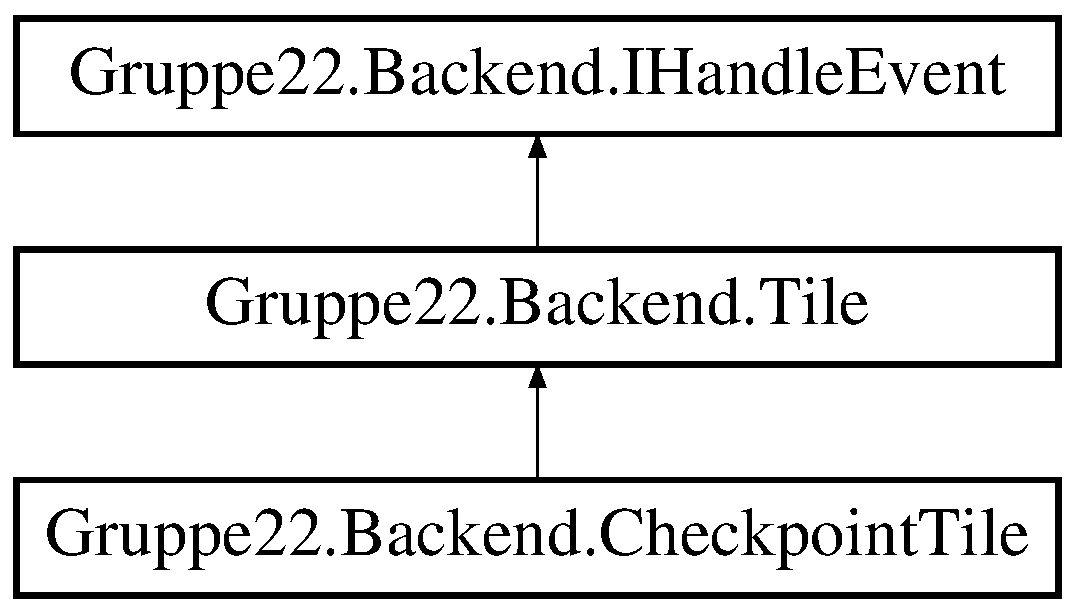
\includegraphics[height=3.000000cm]{class_gruppe22_1_1_backend_1_1_checkpoint_tile}
\end{center}
\end{figure}
\subsection*{Öffentliche Methoden}
\begin{DoxyCompactItemize}
\item 
\hyperlink{class_gruppe22_1_1_backend_1_1_checkpoint_tile_a72935c5b488d2ef10c746a6f0b7ac8ba}{Checkpoint\-Tile} (object \hyperlink{class_gruppe22_1_1_backend_1_1_tile_abc12933c70eb3a2ebbb2fde9f45c2632}{parent}, bool \hyperlink{class_gruppe22_1_1_backend_1_1_checkpoint_tile_a3bbecce1496a23490a6034cb194e6882}{visited}, int \hyperlink{class_gruppe22_1_1_backend_1_1_checkpoint_tile_a4d7e2b4d2acf6d1ca8cff38851e070b7}{bonuslife})
\item 
override void \hyperlink{class_gruppe22_1_1_backend_1_1_checkpoint_tile_adf8bb109a7ea8e8e9e75d63fdac73f36}{Save} (System.\-Xml.\-Xml\-Writer xmlw)
\end{DoxyCompactItemize}
\subsection*{Propertys}
\begin{DoxyCompactItemize}
\item 
bool \hyperlink{class_gruppe22_1_1_backend_1_1_checkpoint_tile_a3bbecce1496a23490a6034cb194e6882}{visited}\hspace{0.3cm}{\ttfamily  \mbox{[}get, set\mbox{]}}
\item 
int \hyperlink{class_gruppe22_1_1_backend_1_1_checkpoint_tile_a4d7e2b4d2acf6d1ca8cff38851e070b7}{bonuslife}\hspace{0.3cm}{\ttfamily  \mbox{[}get, set\mbox{]}}
\end{DoxyCompactItemize}
\subsection*{Weitere Geerbte Elemente}


\subsection{Beschreibung der Konstruktoren und Destruktoren}
\hypertarget{class_gruppe22_1_1_backend_1_1_checkpoint_tile_a72935c5b488d2ef10c746a6f0b7ac8ba}{\index{Gruppe22\-::\-Backend\-::\-Checkpoint\-Tile@{Gruppe22\-::\-Backend\-::\-Checkpoint\-Tile}!Checkpoint\-Tile@{Checkpoint\-Tile}}
\index{Checkpoint\-Tile@{Checkpoint\-Tile}!Gruppe22::Backend::CheckpointTile@{Gruppe22\-::\-Backend\-::\-Checkpoint\-Tile}}
\subsubsection[{Checkpoint\-Tile}]{\setlength{\rightskip}{0pt plus 5cm}Gruppe22.\-Backend.\-Checkpoint\-Tile.\-Checkpoint\-Tile (
\begin{DoxyParamCaption}
\item[{object}]{parent, }
\item[{bool}]{visited, }
\item[{int}]{bonuslife}
\end{DoxyParamCaption}
)}}\label{class_gruppe22_1_1_backend_1_1_checkpoint_tile_a72935c5b488d2ef10c746a6f0b7ac8ba}


\subsection{Dokumentation der Elementfunktionen}
\hypertarget{class_gruppe22_1_1_backend_1_1_checkpoint_tile_adf8bb109a7ea8e8e9e75d63fdac73f36}{\index{Gruppe22\-::\-Backend\-::\-Checkpoint\-Tile@{Gruppe22\-::\-Backend\-::\-Checkpoint\-Tile}!Save@{Save}}
\index{Save@{Save}!Gruppe22::Backend::CheckpointTile@{Gruppe22\-::\-Backend\-::\-Checkpoint\-Tile}}
\subsubsection[{Save}]{\setlength{\rightskip}{0pt plus 5cm}override void Gruppe22.\-Backend.\-Checkpoint\-Tile.\-Save (
\begin{DoxyParamCaption}
\item[{System.\-Xml.\-Xml\-Writer}]{xmlw}
\end{DoxyParamCaption}
)}}\label{class_gruppe22_1_1_backend_1_1_checkpoint_tile_adf8bb109a7ea8e8e9e75d63fdac73f36}


\subsection{Dokumentation der Propertys}
\hypertarget{class_gruppe22_1_1_backend_1_1_checkpoint_tile_a4d7e2b4d2acf6d1ca8cff38851e070b7}{\index{Gruppe22\-::\-Backend\-::\-Checkpoint\-Tile@{Gruppe22\-::\-Backend\-::\-Checkpoint\-Tile}!bonuslife@{bonuslife}}
\index{bonuslife@{bonuslife}!Gruppe22::Backend::CheckpointTile@{Gruppe22\-::\-Backend\-::\-Checkpoint\-Tile}}
\subsubsection[{bonuslife}]{\setlength{\rightskip}{0pt plus 5cm}int Gruppe22.\-Backend.\-Checkpoint\-Tile.\-bonuslife\hspace{0.3cm}{\ttfamily [get]}, {\ttfamily [set]}}}\label{class_gruppe22_1_1_backend_1_1_checkpoint_tile_a4d7e2b4d2acf6d1ca8cff38851e070b7}
\hypertarget{class_gruppe22_1_1_backend_1_1_checkpoint_tile_a3bbecce1496a23490a6034cb194e6882}{\index{Gruppe22\-::\-Backend\-::\-Checkpoint\-Tile@{Gruppe22\-::\-Backend\-::\-Checkpoint\-Tile}!visited@{visited}}
\index{visited@{visited}!Gruppe22::Backend::CheckpointTile@{Gruppe22\-::\-Backend\-::\-Checkpoint\-Tile}}
\subsubsection[{visited}]{\setlength{\rightskip}{0pt plus 5cm}bool Gruppe22.\-Backend.\-Checkpoint\-Tile.\-visited\hspace{0.3cm}{\ttfamily [get]}, {\ttfamily [set]}}}\label{class_gruppe22_1_1_backend_1_1_checkpoint_tile_a3bbecce1496a23490a6034cb194e6882}


Die Dokumentation für diese Klasse wurde erzeugt aufgrund der Datei\-:\begin{DoxyCompactItemize}
\item 
C\-:/\-Users/beursken/\-Documents/\-Git\-Hub/gruppe22/\-Gruppe22/\-Gruppe22/\-Backend/\-Map/\hyperlink{_checkpoint_tile_8cs}{Checkpoint\-Tile.\-cs}\end{DoxyCompactItemize}

\hypertarget{class_dungeon_server_1_1_client_data}{\section{Dungeon\-Server.\-Client\-Data Klassenreferenz}
\label{class_dungeon_server_1_1_client_data}\index{Dungeon\-Server.\-Client\-Data@{Dungeon\-Server.\-Client\-Data}}
}
\subsection*{Öffentliche Methoden}
\begin{DoxyCompactItemize}
\item 
\hyperlink{class_dungeon_server_1_1_client_data_a0fbe7a06af78e568dbe1ee32dd9a2a30}{Client\-Data} (Net\-Connection connection, short id)
\item 
\hyperlink{class_dungeon_server_1_1_client_data_a0aaadda780c18994ef1cc35bf74afe3d}{Client\-Data} (short id)
\end{DoxyCompactItemize}
\subsection*{Öffentliche, statische Methoden}
\begin{DoxyCompactItemize}
\item 
static short \hyperlink{class_dungeon_server_1_1_client_data_aca19f78528851d2fcb837e663ee84f7d}{Get\-Free\-I\-D} (I\-Dictionary$<$ I\-P\-End\-Point, \hyperlink{class_dungeon_server_1_1_client_data}{Client\-Data} $>$ clients)
\end{DoxyCompactItemize}
\subsection*{Propertys}
\begin{DoxyCompactItemize}
\item 
short \hyperlink{class_dungeon_server_1_1_client_data_ac11c0fe5084cdc3d866a036e1258ea67}{I\-D}\hspace{0.3cm}{\ttfamily  \mbox{[}get, set\mbox{]}}
\item 
Net\-Connection \hyperlink{class_dungeon_server_1_1_client_data_a643520d4aba602cd2690cd9bd610a073}{Connection}\hspace{0.3cm}{\ttfamily  \mbox{[}get, set\mbox{]}}
\end{DoxyCompactItemize}


\subsection{Beschreibung der Konstruktoren und Destruktoren}
\hypertarget{class_dungeon_server_1_1_client_data_a0fbe7a06af78e568dbe1ee32dd9a2a30}{\index{Dungeon\-Server\-::\-Client\-Data@{Dungeon\-Server\-::\-Client\-Data}!Client\-Data@{Client\-Data}}
\index{Client\-Data@{Client\-Data}!DungeonServer::ClientData@{Dungeon\-Server\-::\-Client\-Data}}
\subsubsection[{Client\-Data}]{\setlength{\rightskip}{0pt plus 5cm}Dungeon\-Server.\-Client\-Data.\-Client\-Data (
\begin{DoxyParamCaption}
\item[{Net\-Connection}]{connection, }
\item[{short}]{id}
\end{DoxyParamCaption}
)}}\label{class_dungeon_server_1_1_client_data_a0fbe7a06af78e568dbe1ee32dd9a2a30}
\hypertarget{class_dungeon_server_1_1_client_data_a0aaadda780c18994ef1cc35bf74afe3d}{\index{Dungeon\-Server\-::\-Client\-Data@{Dungeon\-Server\-::\-Client\-Data}!Client\-Data@{Client\-Data}}
\index{Client\-Data@{Client\-Data}!DungeonServer::ClientData@{Dungeon\-Server\-::\-Client\-Data}}
\subsubsection[{Client\-Data}]{\setlength{\rightskip}{0pt plus 5cm}Dungeon\-Server.\-Client\-Data.\-Client\-Data (
\begin{DoxyParamCaption}
\item[{short}]{id}
\end{DoxyParamCaption}
)}}\label{class_dungeon_server_1_1_client_data_a0aaadda780c18994ef1cc35bf74afe3d}


\subsection{Dokumentation der Elementfunktionen}
\hypertarget{class_dungeon_server_1_1_client_data_aca19f78528851d2fcb837e663ee84f7d}{\index{Dungeon\-Server\-::\-Client\-Data@{Dungeon\-Server\-::\-Client\-Data}!Get\-Free\-I\-D@{Get\-Free\-I\-D}}
\index{Get\-Free\-I\-D@{Get\-Free\-I\-D}!DungeonServer::ClientData@{Dungeon\-Server\-::\-Client\-Data}}
\subsubsection[{Get\-Free\-I\-D}]{\setlength{\rightskip}{0pt plus 5cm}static short Dungeon\-Server.\-Client\-Data.\-Get\-Free\-I\-D (
\begin{DoxyParamCaption}
\item[{I\-Dictionary$<$ I\-P\-End\-Point, {\bf Client\-Data} $>$}]{clients}
\end{DoxyParamCaption}
)\hspace{0.3cm}{\ttfamily [static]}}}\label{class_dungeon_server_1_1_client_data_aca19f78528851d2fcb837e663ee84f7d}


\subsection{Dokumentation der Propertys}
\hypertarget{class_dungeon_server_1_1_client_data_a643520d4aba602cd2690cd9bd610a073}{\index{Dungeon\-Server\-::\-Client\-Data@{Dungeon\-Server\-::\-Client\-Data}!Connection@{Connection}}
\index{Connection@{Connection}!DungeonServer::ClientData@{Dungeon\-Server\-::\-Client\-Data}}
\subsubsection[{Connection}]{\setlength{\rightskip}{0pt plus 5cm}Net\-Connection Dungeon\-Server.\-Client\-Data.\-Connection\hspace{0.3cm}{\ttfamily [get]}, {\ttfamily [set]}}}\label{class_dungeon_server_1_1_client_data_a643520d4aba602cd2690cd9bd610a073}
\hypertarget{class_dungeon_server_1_1_client_data_ac11c0fe5084cdc3d866a036e1258ea67}{\index{Dungeon\-Server\-::\-Client\-Data@{Dungeon\-Server\-::\-Client\-Data}!I\-D@{I\-D}}
\index{I\-D@{I\-D}!DungeonServer::ClientData@{Dungeon\-Server\-::\-Client\-Data}}
\subsubsection[{I\-D}]{\setlength{\rightskip}{0pt plus 5cm}short Dungeon\-Server.\-Client\-Data.\-I\-D\hspace{0.3cm}{\ttfamily [get]}, {\ttfamily [set]}}}\label{class_dungeon_server_1_1_client_data_ac11c0fe5084cdc3d866a036e1258ea67}


Die Dokumentation für diese Klasse wurde erzeugt aufgrund der Datei\-:\begin{DoxyCompactItemize}
\item 
C\-:/\-Users/beursken/\-Documents/\-Git\-Hub/gruppe22/\-Gruppe22/\-Dungeon\-Server/\hyperlink{_dungeon_server_2_client_data_8cs}{Client\-Data.\-cs}\end{DoxyCompactItemize}

\hypertarget{class_gruppe22_1_1_client_1_1_client_data}{\section{Gruppe22.\-Client.\-Client\-Data Klassenreferenz}
\label{class_gruppe22_1_1_client_1_1_client_data}\index{Gruppe22.\-Client.\-Client\-Data@{Gruppe22.\-Client.\-Client\-Data}}
}
\subsection*{Öffentliche Methoden}
\begin{DoxyCompactItemize}
\item 
\hyperlink{class_gruppe22_1_1_client_1_1_client_data_a79cddbe39d082ab43605afe34418c0da}{Client\-Data} (Net\-Connection connection, short id)
\item 
\hyperlink{class_gruppe22_1_1_client_1_1_client_data_aa4332b19abcafdc627f586c51063004f}{Client\-Data} (short id)
\end{DoxyCompactItemize}
\subsection*{Öffentliche, statische Methoden}
\begin{DoxyCompactItemize}
\item 
static short \hyperlink{class_gruppe22_1_1_client_1_1_client_data_afdd6d5f3a53ecafa6261c2c4f806a261}{Get\-Free\-I\-D} (I\-Dictionary$<$ I\-P\-End\-Point, \hyperlink{class_gruppe22_1_1_client_1_1_client_data}{Client\-Data} $>$ clients)
\end{DoxyCompactItemize}
\subsection*{Propertys}
\begin{DoxyCompactItemize}
\item 
short \hyperlink{class_gruppe22_1_1_client_1_1_client_data_acafb077462c35a4455699df5dac0dc71}{I\-D}\hspace{0.3cm}{\ttfamily  \mbox{[}get, set\mbox{]}}
\item 
Net\-Connection \hyperlink{class_gruppe22_1_1_client_1_1_client_data_a73bd7a2152619a6f3a82c529153e680f}{Connection}\hspace{0.3cm}{\ttfamily  \mbox{[}get, set\mbox{]}}
\end{DoxyCompactItemize}


\subsection{Beschreibung der Konstruktoren und Destruktoren}
\hypertarget{class_gruppe22_1_1_client_1_1_client_data_a79cddbe39d082ab43605afe34418c0da}{\index{Gruppe22\-::\-Client\-::\-Client\-Data@{Gruppe22\-::\-Client\-::\-Client\-Data}!Client\-Data@{Client\-Data}}
\index{Client\-Data@{Client\-Data}!Gruppe22::Client::ClientData@{Gruppe22\-::\-Client\-::\-Client\-Data}}
\subsubsection[{Client\-Data}]{\setlength{\rightskip}{0pt plus 5cm}Gruppe22.\-Client.\-Client\-Data.\-Client\-Data (
\begin{DoxyParamCaption}
\item[{Net\-Connection}]{connection, }
\item[{short}]{id}
\end{DoxyParamCaption}
)}}\label{class_gruppe22_1_1_client_1_1_client_data_a79cddbe39d082ab43605afe34418c0da}
\hypertarget{class_gruppe22_1_1_client_1_1_client_data_aa4332b19abcafdc627f586c51063004f}{\index{Gruppe22\-::\-Client\-::\-Client\-Data@{Gruppe22\-::\-Client\-::\-Client\-Data}!Client\-Data@{Client\-Data}}
\index{Client\-Data@{Client\-Data}!Gruppe22::Client::ClientData@{Gruppe22\-::\-Client\-::\-Client\-Data}}
\subsubsection[{Client\-Data}]{\setlength{\rightskip}{0pt plus 5cm}Gruppe22.\-Client.\-Client\-Data.\-Client\-Data (
\begin{DoxyParamCaption}
\item[{short}]{id}
\end{DoxyParamCaption}
)}}\label{class_gruppe22_1_1_client_1_1_client_data_aa4332b19abcafdc627f586c51063004f}


\subsection{Dokumentation der Elementfunktionen}
\hypertarget{class_gruppe22_1_1_client_1_1_client_data_afdd6d5f3a53ecafa6261c2c4f806a261}{\index{Gruppe22\-::\-Client\-::\-Client\-Data@{Gruppe22\-::\-Client\-::\-Client\-Data}!Get\-Free\-I\-D@{Get\-Free\-I\-D}}
\index{Get\-Free\-I\-D@{Get\-Free\-I\-D}!Gruppe22::Client::ClientData@{Gruppe22\-::\-Client\-::\-Client\-Data}}
\subsubsection[{Get\-Free\-I\-D}]{\setlength{\rightskip}{0pt plus 5cm}static short Gruppe22.\-Client.\-Client\-Data.\-Get\-Free\-I\-D (
\begin{DoxyParamCaption}
\item[{I\-Dictionary$<$ I\-P\-End\-Point, {\bf Client\-Data} $>$}]{clients}
\end{DoxyParamCaption}
)\hspace{0.3cm}{\ttfamily [static]}}}\label{class_gruppe22_1_1_client_1_1_client_data_afdd6d5f3a53ecafa6261c2c4f806a261}


\subsection{Dokumentation der Propertys}
\hypertarget{class_gruppe22_1_1_client_1_1_client_data_a73bd7a2152619a6f3a82c529153e680f}{\index{Gruppe22\-::\-Client\-::\-Client\-Data@{Gruppe22\-::\-Client\-::\-Client\-Data}!Connection@{Connection}}
\index{Connection@{Connection}!Gruppe22::Client::ClientData@{Gruppe22\-::\-Client\-::\-Client\-Data}}
\subsubsection[{Connection}]{\setlength{\rightskip}{0pt plus 5cm}Net\-Connection Gruppe22.\-Client.\-Client\-Data.\-Connection\hspace{0.3cm}{\ttfamily [get]}, {\ttfamily [set]}}}\label{class_gruppe22_1_1_client_1_1_client_data_a73bd7a2152619a6f3a82c529153e680f}
\hypertarget{class_gruppe22_1_1_client_1_1_client_data_acafb077462c35a4455699df5dac0dc71}{\index{Gruppe22\-::\-Client\-::\-Client\-Data@{Gruppe22\-::\-Client\-::\-Client\-Data}!I\-D@{I\-D}}
\index{I\-D@{I\-D}!Gruppe22::Client::ClientData@{Gruppe22\-::\-Client\-::\-Client\-Data}}
\subsubsection[{I\-D}]{\setlength{\rightskip}{0pt plus 5cm}short Gruppe22.\-Client.\-Client\-Data.\-I\-D\hspace{0.3cm}{\ttfamily [get]}, {\ttfamily [set]}}}\label{class_gruppe22_1_1_client_1_1_client_data_acafb077462c35a4455699df5dac0dc71}


Die Dokumentation für diese Klasse wurde erzeugt aufgrund der Datei\-:\begin{DoxyCompactItemize}
\item 
C\-:/\-Users/beursken/\-Documents/\-Git\-Hub/gruppe22/\-Gruppe22/\-Gruppe22/\-Client/\-U\-I/\hyperlink{_gruppe22_2_client_2_u_i_2_client_data_8cs}{Client\-Data.\-cs}\end{DoxyCompactItemize}

\hypertarget{class_gruppe22_1_1_backend_1_1_coords}{\section{Gruppe22.\-Backend.\-Coords Klassenreferenz}
\label{class_gruppe22_1_1_backend_1_1_coords}\index{Gruppe22.\-Backend.\-Coords@{Gruppe22.\-Backend.\-Coords}}
}


A two dimensional coordinate  


Klassendiagramm für Gruppe22.\-Backend.\-Coords\-:\begin{figure}[H]
\begin{center}
\leavevmode
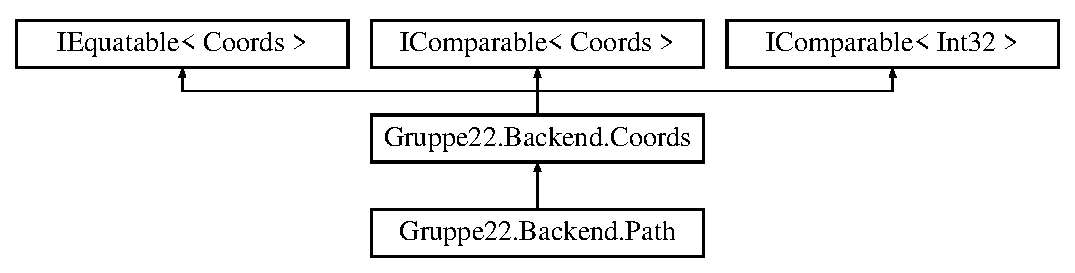
\includegraphics[height=3.000000cm]{class_gruppe22_1_1_backend_1_1_coords}
\end{center}
\end{figure}
\subsection*{Öffentliche Methoden}
\begin{DoxyCompactItemize}
\item 
int \hyperlink{class_gruppe22_1_1_backend_1_1_coords_af1e05666f06a514626fb624381b20188}{Distance\-From} (\hyperlink{class_gruppe22_1_1_backend_1_1_coords}{Coords} coords)
\item 
int \hyperlink{class_gruppe22_1_1_backend_1_1_coords_a80e44f8ce720c800294ea7767c8ad2d4}{Distance\-From} (int \hyperlink{class_gruppe22_1_1_backend_1_1_coords_a5d6a2857d47b7fb03ff0fa9c07a41d11}{x}, int \hyperlink{class_gruppe22_1_1_backend_1_1_coords_a941b0ec77fa0973cc2faf35f9a6d85dd}{y})
\item 
override int \hyperlink{class_gruppe22_1_1_backend_1_1_coords_a330a4754be4e5d50c2efa07d046a2b9b}{Get\-Hash\-Code} ()
\item 
override bool \hyperlink{class_gruppe22_1_1_backend_1_1_coords_a294cf31d438e861ef2e2d9d3d6068b4f}{Equals} (object obj)
\item 
override string \hyperlink{class_gruppe22_1_1_backend_1_1_coords_a25e055e9bf0d25318f30b3611cdee050}{To\-String} ()
\item 
\hyperlink{class_gruppe22_1_1_backend_1_1_coords_a5f2dabc4615c0de75c0e50ca709df6bc}{Coords} (int \hyperlink{class_gruppe22_1_1_backend_1_1_coords_a5d6a2857d47b7fb03ff0fa9c07a41d11}{x}=-\/1, int \hyperlink{class_gruppe22_1_1_backend_1_1_coords_a941b0ec77fa0973cc2faf35f9a6d85dd}{y}=-\/1)
\begin{DoxyCompactList}\small\item\em Creates a new two dimensional point \end{DoxyCompactList}\item 
\hyperlink{class_gruppe22_1_1_backend_1_1_coords_a4f39203cb05943723de094a3ec8bd29d}{Coords} (Vector2 \hyperlink{class_gruppe22_1_1_backend_1_1_coords_a44af20a66f196320d537beed94622ce4}{vector})
\item 
bool \hyperlink{class_gruppe22_1_1_backend_1_1_coords_ad5aae2d517c9e3916da5f2d6874737dc}{Equals} (\hyperlink{class_gruppe22_1_1_backend_1_1_coords}{Coords} other)
\item 
int \hyperlink{class_gruppe22_1_1_backend_1_1_coords_ad09860f971ff478900daeb4337dbec6f}{Compare\-To} (\hyperlink{class_gruppe22_1_1_backend_1_1_coords}{Coords} other)
\item 
int \hyperlink{class_gruppe22_1_1_backend_1_1_coords_a9cb8c0ad330e5d405c7037f163fa122f}{Compare\-To} (int other)
\end{DoxyCompactItemize}
\subsection*{Öffentliche, statische Methoden}
\begin{DoxyCompactItemize}
\item 
static \hyperlink{class_gruppe22_1_1_backend_1_1_coords}{Coords} \hyperlink{class_gruppe22_1_1_backend_1_1_coords_a300f68b47e61012007f61383a1a23cd3}{operator+} (\hyperlink{class_gruppe22_1_1_backend_1_1_coords}{Coords} c1, \hyperlink{class_gruppe22_1_1_backend_1_1_coords}{Backend.\-Coords} c2)
\item 
static bool \hyperlink{class_gruppe22_1_1_backend_1_1_coords_afda506d3a645625175835c78e64cc325}{operator!=} (\hyperlink{class_gruppe22_1_1_backend_1_1_coords}{Coords} c1, \hyperlink{class_gruppe22_1_1_backend_1_1_coords}{Backend.\-Coords} c2)
\item 
static bool \hyperlink{class_gruppe22_1_1_backend_1_1_coords_a79eefabf66131259ce0d0fecd10a7cc3}{operator==} (\hyperlink{class_gruppe22_1_1_backend_1_1_coords}{Coords} c1, \hyperlink{class_gruppe22_1_1_backend_1_1_coords}{Backend.\-Coords} c2)
\end{DoxyCompactItemize}
\subsection*{Propertys}
\begin{DoxyCompactItemize}
\item 
int \hyperlink{class_gruppe22_1_1_backend_1_1_coords_a5d6a2857d47b7fb03ff0fa9c07a41d11}{x}\hspace{0.3cm}{\ttfamily  \mbox{[}get, set\mbox{]}}
\begin{DoxyCompactList}\small\item\em Current x coordinate \end{DoxyCompactList}\item 
int \hyperlink{class_gruppe22_1_1_backend_1_1_coords_a941b0ec77fa0973cc2faf35f9a6d85dd}{y}\hspace{0.3cm}{\ttfamily  \mbox{[}get, set\mbox{]}}
\begin{DoxyCompactList}\small\item\em Current y coordinate \end{DoxyCompactList}\item 
Vector2 \hyperlink{class_gruppe22_1_1_backend_1_1_coords_a44af20a66f196320d537beed94622ce4}{vector}\hspace{0.3cm}{\ttfamily  \mbox{[}get, set\mbox{]}}
\item 
static \hyperlink{class_gruppe22_1_1_backend_1_1_coords}{Coords} \hyperlink{class_gruppe22_1_1_backend_1_1_coords_ac2aea2e761ea4b4c95ef1667eb8dfaf8}{Zero}\hspace{0.3cm}{\ttfamily  \mbox{[}get\mbox{]}}
\end{DoxyCompactItemize}


\subsection{Ausführliche Beschreibung}
A two dimensional coordinate 



\subsection{Beschreibung der Konstruktoren und Destruktoren}
\hypertarget{class_gruppe22_1_1_backend_1_1_coords_a5f2dabc4615c0de75c0e50ca709df6bc}{\index{Gruppe22\-::\-Backend\-::\-Coords@{Gruppe22\-::\-Backend\-::\-Coords}!Coords@{Coords}}
\index{Coords@{Coords}!Gruppe22::Backend::Coords@{Gruppe22\-::\-Backend\-::\-Coords}}
\subsubsection[{Coords}]{\setlength{\rightskip}{0pt plus 5cm}Gruppe22.\-Backend.\-Coords.\-Coords (
\begin{DoxyParamCaption}
\item[{int}]{x = {\ttfamily -\/1}, }
\item[{int}]{y = {\ttfamily -\/1}}
\end{DoxyParamCaption}
)}}\label{class_gruppe22_1_1_backend_1_1_coords_a5f2dabc4615c0de75c0e50ca709df6bc}


Creates a new two dimensional point 


\begin{DoxyParams}{Parameter}
{\em x} & X-\/coordinate (default\-:-\/1)\\
\hline
{\em y} & Y-\/coordinate (default\-:-\/1)\\
\hline
\end{DoxyParams}
\hypertarget{class_gruppe22_1_1_backend_1_1_coords_a4f39203cb05943723de094a3ec8bd29d}{\index{Gruppe22\-::\-Backend\-::\-Coords@{Gruppe22\-::\-Backend\-::\-Coords}!Coords@{Coords}}
\index{Coords@{Coords}!Gruppe22::Backend::Coords@{Gruppe22\-::\-Backend\-::\-Coords}}
\subsubsection[{Coords}]{\setlength{\rightskip}{0pt plus 5cm}Gruppe22.\-Backend.\-Coords.\-Coords (
\begin{DoxyParamCaption}
\item[{Vector2}]{vector}
\end{DoxyParamCaption}
)}}\label{class_gruppe22_1_1_backend_1_1_coords_a4f39203cb05943723de094a3ec8bd29d}


\subsection{Dokumentation der Elementfunktionen}
\hypertarget{class_gruppe22_1_1_backend_1_1_coords_ad09860f971ff478900daeb4337dbec6f}{\index{Gruppe22\-::\-Backend\-::\-Coords@{Gruppe22\-::\-Backend\-::\-Coords}!Compare\-To@{Compare\-To}}
\index{Compare\-To@{Compare\-To}!Gruppe22::Backend::Coords@{Gruppe22\-::\-Backend\-::\-Coords}}
\subsubsection[{Compare\-To}]{\setlength{\rightskip}{0pt plus 5cm}int Gruppe22.\-Backend.\-Coords.\-Compare\-To (
\begin{DoxyParamCaption}
\item[{{\bf Coords}}]{other}
\end{DoxyParamCaption}
)}}\label{class_gruppe22_1_1_backend_1_1_coords_ad09860f971ff478900daeb4337dbec6f}
\hypertarget{class_gruppe22_1_1_backend_1_1_coords_a9cb8c0ad330e5d405c7037f163fa122f}{\index{Gruppe22\-::\-Backend\-::\-Coords@{Gruppe22\-::\-Backend\-::\-Coords}!Compare\-To@{Compare\-To}}
\index{Compare\-To@{Compare\-To}!Gruppe22::Backend::Coords@{Gruppe22\-::\-Backend\-::\-Coords}}
\subsubsection[{Compare\-To}]{\setlength{\rightskip}{0pt plus 5cm}int Gruppe22.\-Backend.\-Coords.\-Compare\-To (
\begin{DoxyParamCaption}
\item[{int}]{other}
\end{DoxyParamCaption}
)}}\label{class_gruppe22_1_1_backend_1_1_coords_a9cb8c0ad330e5d405c7037f163fa122f}
\hypertarget{class_gruppe22_1_1_backend_1_1_coords_af1e05666f06a514626fb624381b20188}{\index{Gruppe22\-::\-Backend\-::\-Coords@{Gruppe22\-::\-Backend\-::\-Coords}!Distance\-From@{Distance\-From}}
\index{Distance\-From@{Distance\-From}!Gruppe22::Backend::Coords@{Gruppe22\-::\-Backend\-::\-Coords}}
\subsubsection[{Distance\-From}]{\setlength{\rightskip}{0pt plus 5cm}int Gruppe22.\-Backend.\-Coords.\-Distance\-From (
\begin{DoxyParamCaption}
\item[{{\bf Coords}}]{coords}
\end{DoxyParamCaption}
)}}\label{class_gruppe22_1_1_backend_1_1_coords_af1e05666f06a514626fb624381b20188}
\hypertarget{class_gruppe22_1_1_backend_1_1_coords_a80e44f8ce720c800294ea7767c8ad2d4}{\index{Gruppe22\-::\-Backend\-::\-Coords@{Gruppe22\-::\-Backend\-::\-Coords}!Distance\-From@{Distance\-From}}
\index{Distance\-From@{Distance\-From}!Gruppe22::Backend::Coords@{Gruppe22\-::\-Backend\-::\-Coords}}
\subsubsection[{Distance\-From}]{\setlength{\rightskip}{0pt plus 5cm}int Gruppe22.\-Backend.\-Coords.\-Distance\-From (
\begin{DoxyParamCaption}
\item[{int}]{x, }
\item[{int}]{y}
\end{DoxyParamCaption}
)}}\label{class_gruppe22_1_1_backend_1_1_coords_a80e44f8ce720c800294ea7767c8ad2d4}
\hypertarget{class_gruppe22_1_1_backend_1_1_coords_a294cf31d438e861ef2e2d9d3d6068b4f}{\index{Gruppe22\-::\-Backend\-::\-Coords@{Gruppe22\-::\-Backend\-::\-Coords}!Equals@{Equals}}
\index{Equals@{Equals}!Gruppe22::Backend::Coords@{Gruppe22\-::\-Backend\-::\-Coords}}
\subsubsection[{Equals}]{\setlength{\rightskip}{0pt plus 5cm}override bool Gruppe22.\-Backend.\-Coords.\-Equals (
\begin{DoxyParamCaption}
\item[{object}]{obj}
\end{DoxyParamCaption}
)}}\label{class_gruppe22_1_1_backend_1_1_coords_a294cf31d438e861ef2e2d9d3d6068b4f}
\hypertarget{class_gruppe22_1_1_backend_1_1_coords_ad5aae2d517c9e3916da5f2d6874737dc}{\index{Gruppe22\-::\-Backend\-::\-Coords@{Gruppe22\-::\-Backend\-::\-Coords}!Equals@{Equals}}
\index{Equals@{Equals}!Gruppe22::Backend::Coords@{Gruppe22\-::\-Backend\-::\-Coords}}
\subsubsection[{Equals}]{\setlength{\rightskip}{0pt plus 5cm}bool Gruppe22.\-Backend.\-Coords.\-Equals (
\begin{DoxyParamCaption}
\item[{{\bf Coords}}]{other}
\end{DoxyParamCaption}
)}}\label{class_gruppe22_1_1_backend_1_1_coords_ad5aae2d517c9e3916da5f2d6874737dc}
\hypertarget{class_gruppe22_1_1_backend_1_1_coords_a330a4754be4e5d50c2efa07d046a2b9b}{\index{Gruppe22\-::\-Backend\-::\-Coords@{Gruppe22\-::\-Backend\-::\-Coords}!Get\-Hash\-Code@{Get\-Hash\-Code}}
\index{Get\-Hash\-Code@{Get\-Hash\-Code}!Gruppe22::Backend::Coords@{Gruppe22\-::\-Backend\-::\-Coords}}
\subsubsection[{Get\-Hash\-Code}]{\setlength{\rightskip}{0pt plus 5cm}override int Gruppe22.\-Backend.\-Coords.\-Get\-Hash\-Code (
\begin{DoxyParamCaption}
{}
\end{DoxyParamCaption}
)}}\label{class_gruppe22_1_1_backend_1_1_coords_a330a4754be4e5d50c2efa07d046a2b9b}
\hypertarget{class_gruppe22_1_1_backend_1_1_coords_afda506d3a645625175835c78e64cc325}{\index{Gruppe22\-::\-Backend\-::\-Coords@{Gruppe22\-::\-Backend\-::\-Coords}!operator!=@{operator!=}}
\index{operator!=@{operator!=}!Gruppe22::Backend::Coords@{Gruppe22\-::\-Backend\-::\-Coords}}
\subsubsection[{operator!=}]{\setlength{\rightskip}{0pt plus 5cm}static bool Gruppe22.\-Backend.\-Coords.\-operator!= (
\begin{DoxyParamCaption}
\item[{{\bf Coords}}]{c1, }
\item[{{\bf Backend.\-Coords}}]{c2}
\end{DoxyParamCaption}
)\hspace{0.3cm}{\ttfamily [static]}}}\label{class_gruppe22_1_1_backend_1_1_coords_afda506d3a645625175835c78e64cc325}
\hypertarget{class_gruppe22_1_1_backend_1_1_coords_a300f68b47e61012007f61383a1a23cd3}{\index{Gruppe22\-::\-Backend\-::\-Coords@{Gruppe22\-::\-Backend\-::\-Coords}!operator+@{operator+}}
\index{operator+@{operator+}!Gruppe22::Backend::Coords@{Gruppe22\-::\-Backend\-::\-Coords}}
\subsubsection[{operator+}]{\setlength{\rightskip}{0pt plus 5cm}static {\bf Coords} Gruppe22.\-Backend.\-Coords.\-operator+ (
\begin{DoxyParamCaption}
\item[{{\bf Coords}}]{c1, }
\item[{{\bf Backend.\-Coords}}]{c2}
\end{DoxyParamCaption}
)\hspace{0.3cm}{\ttfamily [static]}}}\label{class_gruppe22_1_1_backend_1_1_coords_a300f68b47e61012007f61383a1a23cd3}
\hypertarget{class_gruppe22_1_1_backend_1_1_coords_a79eefabf66131259ce0d0fecd10a7cc3}{\index{Gruppe22\-::\-Backend\-::\-Coords@{Gruppe22\-::\-Backend\-::\-Coords}!operator==@{operator==}}
\index{operator==@{operator==}!Gruppe22::Backend::Coords@{Gruppe22\-::\-Backend\-::\-Coords}}
\subsubsection[{operator==}]{\setlength{\rightskip}{0pt plus 5cm}static bool Gruppe22.\-Backend.\-Coords.\-operator== (
\begin{DoxyParamCaption}
\item[{{\bf Coords}}]{c1, }
\item[{{\bf Backend.\-Coords}}]{c2}
\end{DoxyParamCaption}
)\hspace{0.3cm}{\ttfamily [static]}}}\label{class_gruppe22_1_1_backend_1_1_coords_a79eefabf66131259ce0d0fecd10a7cc3}
\hypertarget{class_gruppe22_1_1_backend_1_1_coords_a25e055e9bf0d25318f30b3611cdee050}{\index{Gruppe22\-::\-Backend\-::\-Coords@{Gruppe22\-::\-Backend\-::\-Coords}!To\-String@{To\-String}}
\index{To\-String@{To\-String}!Gruppe22::Backend::Coords@{Gruppe22\-::\-Backend\-::\-Coords}}
\subsubsection[{To\-String}]{\setlength{\rightskip}{0pt plus 5cm}override string Gruppe22.\-Backend.\-Coords.\-To\-String (
\begin{DoxyParamCaption}
{}
\end{DoxyParamCaption}
)}}\label{class_gruppe22_1_1_backend_1_1_coords_a25e055e9bf0d25318f30b3611cdee050}


\subsection{Dokumentation der Propertys}
\hypertarget{class_gruppe22_1_1_backend_1_1_coords_a44af20a66f196320d537beed94622ce4}{\index{Gruppe22\-::\-Backend\-::\-Coords@{Gruppe22\-::\-Backend\-::\-Coords}!vector@{vector}}
\index{vector@{vector}!Gruppe22::Backend::Coords@{Gruppe22\-::\-Backend\-::\-Coords}}
\subsubsection[{vector}]{\setlength{\rightskip}{0pt plus 5cm}Vector2 Gruppe22.\-Backend.\-Coords.\-vector\hspace{0.3cm}{\ttfamily [get]}, {\ttfamily [set]}}}\label{class_gruppe22_1_1_backend_1_1_coords_a44af20a66f196320d537beed94622ce4}
\hypertarget{class_gruppe22_1_1_backend_1_1_coords_a5d6a2857d47b7fb03ff0fa9c07a41d11}{\index{Gruppe22\-::\-Backend\-::\-Coords@{Gruppe22\-::\-Backend\-::\-Coords}!x@{x}}
\index{x@{x}!Gruppe22::Backend::Coords@{Gruppe22\-::\-Backend\-::\-Coords}}
\subsubsection[{x}]{\setlength{\rightskip}{0pt plus 5cm}int Gruppe22.\-Backend.\-Coords.\-x\hspace{0.3cm}{\ttfamily [get]}, {\ttfamily [set]}}}\label{class_gruppe22_1_1_backend_1_1_coords_a5d6a2857d47b7fb03ff0fa9c07a41d11}


Current x coordinate 

\hypertarget{class_gruppe22_1_1_backend_1_1_coords_a941b0ec77fa0973cc2faf35f9a6d85dd}{\index{Gruppe22\-::\-Backend\-::\-Coords@{Gruppe22\-::\-Backend\-::\-Coords}!y@{y}}
\index{y@{y}!Gruppe22::Backend::Coords@{Gruppe22\-::\-Backend\-::\-Coords}}
\subsubsection[{y}]{\setlength{\rightskip}{0pt plus 5cm}int Gruppe22.\-Backend.\-Coords.\-y\hspace{0.3cm}{\ttfamily [get]}, {\ttfamily [set]}}}\label{class_gruppe22_1_1_backend_1_1_coords_a941b0ec77fa0973cc2faf35f9a6d85dd}


Current y coordinate 

\hypertarget{class_gruppe22_1_1_backend_1_1_coords_ac2aea2e761ea4b4c95ef1667eb8dfaf8}{\index{Gruppe22\-::\-Backend\-::\-Coords@{Gruppe22\-::\-Backend\-::\-Coords}!Zero@{Zero}}
\index{Zero@{Zero}!Gruppe22::Backend::Coords@{Gruppe22\-::\-Backend\-::\-Coords}}
\subsubsection[{Zero}]{\setlength{\rightskip}{0pt plus 5cm}{\bf Coords} Gruppe22.\-Backend.\-Coords.\-Zero\hspace{0.3cm}{\ttfamily [static]}, {\ttfamily [get]}}}\label{class_gruppe22_1_1_backend_1_1_coords_ac2aea2e761ea4b4c95ef1667eb8dfaf8}


Die Dokumentation für diese Klasse wurde erzeugt aufgrund der Datei\-:\begin{DoxyCompactItemize}
\item 
C\-:/\-Users/beursken/\-Documents/\-Git\-Hub/gruppe22/\-Gruppe22/\-Gruppe22/\-Backend/\hyperlink{_helpers_8cs}{Helpers.\-cs}\end{DoxyCompactItemize}

\hypertarget{class_gruppe22_1_1_client_1_1_create_x_m_l_files}{\section{Gruppe22.\-Client.\-Create\-X\-M\-L\-Files Klassenreferenz}
\label{class_gruppe22_1_1_client_1_1_create_x_m_l_files}\index{Gruppe22.\-Client.\-Create\-X\-M\-L\-Files@{Gruppe22.\-Client.\-Create\-X\-M\-L\-Files}}
}
\subsection*{Öffentliche, statische Methoden}
\begin{DoxyCompactItemize}
\item 
static async Task \hyperlink{class_gruppe22_1_1_client_1_1_create_x_m_l_files_af39075e03392991cba8d00d0724b840e}{Create\-X\-M\-L} (\hyperlink{class_gruppe22_1_1_client_1_1_mainmap}{Mainmap} \-\_\-map, \hyperlink{class_gruppe22_1_1_client_1_1_camera}{Camera} \-\_\-camera, Content\-Manager \-\_\-content)
\item 
static void \hyperlink{class_gruppe22_1_1_client_1_1_create_x_m_l_files_a27cc4bd6249a50b449ec4a365b23a773}{Create\-Actor} (\hyperlink{class_gruppe22_1_1_client_1_1_mainmap}{Mainmap} \-\_\-map, Content\-Manager \-\_\-content, \hyperlink{class_gruppe22_1_1_client_1_1_camera}{Camera} \-\_\-camera, string character=\char`\"{}\char`\"{})
\item 
static void \hyperlink{class_gruppe22_1_1_client_1_1_create_x_m_l_files_a58457d31a59c1e2caf9ecb5c8b722f52}{Create\-Walls} (Content\-Manager \-\_\-content, string name)
\item 
static void \hyperlink{class_gruppe22_1_1_client_1_1_create_x_m_l_files_ac83bee8eae267e40e976d6d665b0beb2}{Create\-Floor} (Content\-Manager \-\_\-content, string name)
\item 
static void \hyperlink{class_gruppe22_1_1_client_1_1_create_x_m_l_files_a9de979b9106c7528fdd849dcc59b0625}{Create\-Mix} (Content\-Manager \-\_\-content)
\end{DoxyCompactItemize}


\subsection{Dokumentation der Elementfunktionen}
\hypertarget{class_gruppe22_1_1_client_1_1_create_x_m_l_files_a27cc4bd6249a50b449ec4a365b23a773}{\index{Gruppe22\-::\-Client\-::\-Create\-X\-M\-L\-Files@{Gruppe22\-::\-Client\-::\-Create\-X\-M\-L\-Files}!Create\-Actor@{Create\-Actor}}
\index{Create\-Actor@{Create\-Actor}!Gruppe22::Client::CreateXMLFiles@{Gruppe22\-::\-Client\-::\-Create\-X\-M\-L\-Files}}
\subsubsection[{Create\-Actor}]{\setlength{\rightskip}{0pt plus 5cm}static void Gruppe22.\-Client.\-Create\-X\-M\-L\-Files.\-Create\-Actor (
\begin{DoxyParamCaption}
\item[{{\bf Mainmap}}]{\-\_\-map, }
\item[{Content\-Manager}]{\-\_\-content, }
\item[{{\bf Camera}}]{\-\_\-camera, }
\item[{string}]{character = {\ttfamily \char`\"{}\char`\"{}}}
\end{DoxyParamCaption}
)\hspace{0.3cm}{\ttfamily [static]}}}\label{class_gruppe22_1_1_client_1_1_create_x_m_l_files_a27cc4bd6249a50b449ec4a365b23a773}
\hypertarget{class_gruppe22_1_1_client_1_1_create_x_m_l_files_ac83bee8eae267e40e976d6d665b0beb2}{\index{Gruppe22\-::\-Client\-::\-Create\-X\-M\-L\-Files@{Gruppe22\-::\-Client\-::\-Create\-X\-M\-L\-Files}!Create\-Floor@{Create\-Floor}}
\index{Create\-Floor@{Create\-Floor}!Gruppe22::Client::CreateXMLFiles@{Gruppe22\-::\-Client\-::\-Create\-X\-M\-L\-Files}}
\subsubsection[{Create\-Floor}]{\setlength{\rightskip}{0pt plus 5cm}static void Gruppe22.\-Client.\-Create\-X\-M\-L\-Files.\-Create\-Floor (
\begin{DoxyParamCaption}
\item[{Content\-Manager}]{\-\_\-content, }
\item[{string}]{name}
\end{DoxyParamCaption}
)\hspace{0.3cm}{\ttfamily [static]}}}\label{class_gruppe22_1_1_client_1_1_create_x_m_l_files_ac83bee8eae267e40e976d6d665b0beb2}
\hypertarget{class_gruppe22_1_1_client_1_1_create_x_m_l_files_a9de979b9106c7528fdd849dcc59b0625}{\index{Gruppe22\-::\-Client\-::\-Create\-X\-M\-L\-Files@{Gruppe22\-::\-Client\-::\-Create\-X\-M\-L\-Files}!Create\-Mix@{Create\-Mix}}
\index{Create\-Mix@{Create\-Mix}!Gruppe22::Client::CreateXMLFiles@{Gruppe22\-::\-Client\-::\-Create\-X\-M\-L\-Files}}
\subsubsection[{Create\-Mix}]{\setlength{\rightskip}{0pt plus 5cm}static void Gruppe22.\-Client.\-Create\-X\-M\-L\-Files.\-Create\-Mix (
\begin{DoxyParamCaption}
\item[{Content\-Manager}]{\-\_\-content}
\end{DoxyParamCaption}
)\hspace{0.3cm}{\ttfamily [static]}}}\label{class_gruppe22_1_1_client_1_1_create_x_m_l_files_a9de979b9106c7528fdd849dcc59b0625}
\hypertarget{class_gruppe22_1_1_client_1_1_create_x_m_l_files_a58457d31a59c1e2caf9ecb5c8b722f52}{\index{Gruppe22\-::\-Client\-::\-Create\-X\-M\-L\-Files@{Gruppe22\-::\-Client\-::\-Create\-X\-M\-L\-Files}!Create\-Walls@{Create\-Walls}}
\index{Create\-Walls@{Create\-Walls}!Gruppe22::Client::CreateXMLFiles@{Gruppe22\-::\-Client\-::\-Create\-X\-M\-L\-Files}}
\subsubsection[{Create\-Walls}]{\setlength{\rightskip}{0pt plus 5cm}static void Gruppe22.\-Client.\-Create\-X\-M\-L\-Files.\-Create\-Walls (
\begin{DoxyParamCaption}
\item[{Content\-Manager}]{\-\_\-content, }
\item[{string}]{name}
\end{DoxyParamCaption}
)\hspace{0.3cm}{\ttfamily [static]}}}\label{class_gruppe22_1_1_client_1_1_create_x_m_l_files_a58457d31a59c1e2caf9ecb5c8b722f52}
\hypertarget{class_gruppe22_1_1_client_1_1_create_x_m_l_files_af39075e03392991cba8d00d0724b840e}{\index{Gruppe22\-::\-Client\-::\-Create\-X\-M\-L\-Files@{Gruppe22\-::\-Client\-::\-Create\-X\-M\-L\-Files}!Create\-X\-M\-L@{Create\-X\-M\-L}}
\index{Create\-X\-M\-L@{Create\-X\-M\-L}!Gruppe22::Client::CreateXMLFiles@{Gruppe22\-::\-Client\-::\-Create\-X\-M\-L\-Files}}
\subsubsection[{Create\-X\-M\-L}]{\setlength{\rightskip}{0pt plus 5cm}static async Task Gruppe22.\-Client.\-Create\-X\-M\-L\-Files.\-Create\-X\-M\-L (
\begin{DoxyParamCaption}
\item[{{\bf Mainmap}}]{\-\_\-map, }
\item[{{\bf Camera}}]{\-\_\-camera, }
\item[{Content\-Manager}]{\-\_\-content}
\end{DoxyParamCaption}
)\hspace{0.3cm}{\ttfamily [static]}}}\label{class_gruppe22_1_1_client_1_1_create_x_m_l_files_af39075e03392991cba8d00d0724b840e}


Die Dokumentation für diese Klasse wurde erzeugt aufgrund der Datei\-:\begin{DoxyCompactItemize}
\item 
C\-:/\-Users/beursken/\-Documents/\-Git\-Hub/gruppe22/\-Gruppe22/\-Gruppe22/\-Client/\-Map/\hyperlink{_create_x_m_l_files_8cs}{Create\-X\-M\-L\-Files.\-cs}\end{DoxyCompactItemize}

\hypertarget{class_gruppe22_1_1_client_1_1_dialog}{\section{Gruppe22.\-Client.\-Dialog Klassenreferenz}
\label{class_gruppe22_1_1_client_1_1_dialog}\index{Gruppe22.\-Client.\-Dialog@{Gruppe22.\-Client.\-Dialog}}
}
Klassendiagramm für Gruppe22.\-Client.\-Dialog\-:\begin{figure}[H]
\begin{center}
\leavevmode
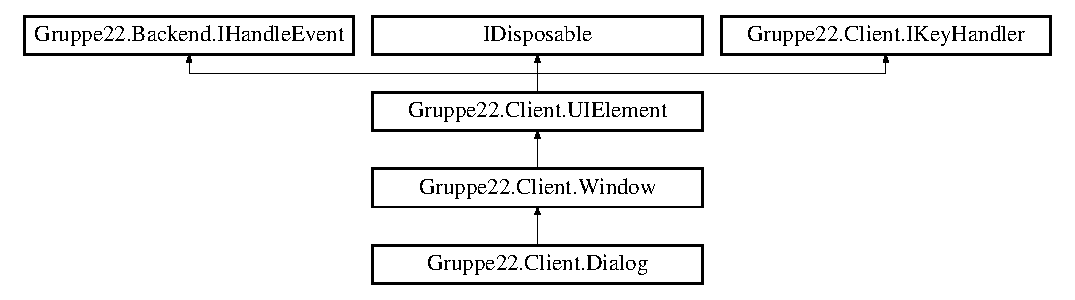
\includegraphics[height=3.589744cm]{class_gruppe22_1_1_client_1_1_dialog}
\end{center}
\end{figure}
\subsection*{Öffentliche Methoden}
\begin{DoxyCompactItemize}
\item 
\hyperlink{class_gruppe22_1_1_client_1_1_dialog_a4cc28aa4711abd90a9c16d85464ca192}{Dialog} (\hyperlink{interface_gruppe22_1_1_backend_1_1_i_handle_event}{Backend.\-I\-Handle\-Event} parent, Sprite\-Batch sprite\-Batch, Content\-Manager content, Rectangle display\-Rect, \hyperlink{class_gruppe22_1_1_backend_1_1_actor}{Backend.\-Actor} actor)
\begin{DoxyCompactList}\small\item\em Constructor \end{DoxyCompactList}\end{DoxyCompactItemize}
\subsection*{Weitere Geerbte Elemente}


\subsection{Beschreibung der Konstruktoren und Destruktoren}
\hypertarget{class_gruppe22_1_1_client_1_1_dialog_a4cc28aa4711abd90a9c16d85464ca192}{\index{Gruppe22\-::\-Client\-::\-Dialog@{Gruppe22\-::\-Client\-::\-Dialog}!Dialog@{Dialog}}
\index{Dialog@{Dialog}!Gruppe22::Client::Dialog@{Gruppe22\-::\-Client\-::\-Dialog}}
\subsubsection[{Dialog}]{\setlength{\rightskip}{0pt plus 5cm}Gruppe22.\-Client.\-Dialog.\-Dialog (
\begin{DoxyParamCaption}
\item[{{\bf Backend.\-I\-Handle\-Event}}]{parent, }
\item[{Sprite\-Batch}]{sprite\-Batch, }
\item[{Content\-Manager}]{content, }
\item[{Rectangle}]{display\-Rect, }
\item[{{\bf Backend.\-Actor}}]{actor}
\end{DoxyParamCaption}
)}}\label{class_gruppe22_1_1_client_1_1_dialog_a4cc28aa4711abd90a9c16d85464ca192}


Constructor 



Die Dokumentation für diese Klasse wurde erzeugt aufgrund der Datei\-:\begin{DoxyCompactItemize}
\item 
C\-:/\-Users/beursken/\-Documents/\-Git\-Hub/gruppe22/\-Gruppe22/\-Gruppe22/\-Client/\-U\-I/\hyperlink{_dialog_8cs}{Dialog.\-cs}\end{DoxyCompactItemize}

\hypertarget{class_gruppe22_1_1_backend_1_1_door_tile}{\section{Gruppe22.\-Backend.\-Door\-Tile Klassenreferenz}
\label{class_gruppe22_1_1_backend_1_1_door_tile}\index{Gruppe22.\-Backend.\-Door\-Tile@{Gruppe22.\-Backend.\-Door\-Tile}}
}
Klassendiagramm für Gruppe22.\-Backend.\-Door\-Tile\-:\begin{figure}[H]
\begin{center}
\leavevmode
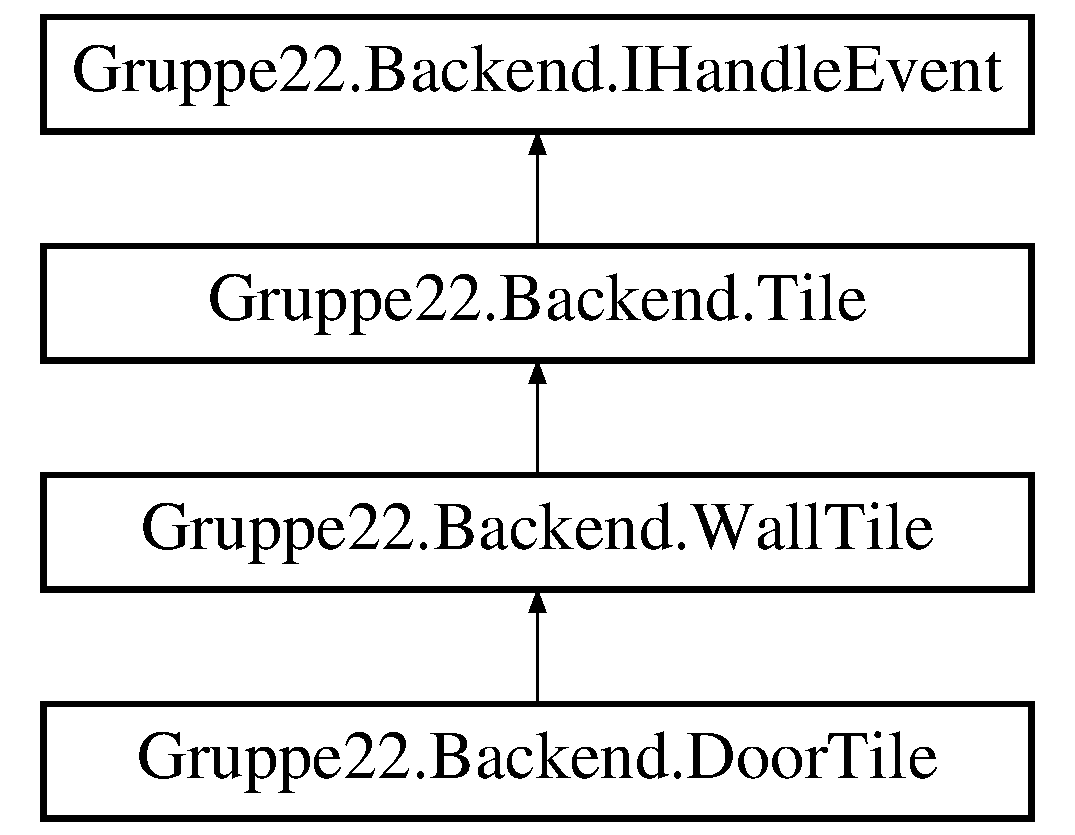
\includegraphics[height=4.000000cm]{class_gruppe22_1_1_backend_1_1_door_tile}
\end{center}
\end{figure}
\subsection*{Öffentliche Methoden}
\begin{DoxyCompactItemize}
\item 
\hyperlink{class_gruppe22_1_1_backend_1_1_door_tile_ab0e5117c31167d0107e0b677d2ea09b4}{Door\-Tile} (object \hyperlink{class_gruppe22_1_1_backend_1_1_tile_abc12933c70eb3a2ebbb2fde9f45c2632}{parent}, bool locked=true, int \hyperlink{class_gruppe22_1_1_backend_1_1_door_tile_a25b6d03598ee1e0d2fab39b77586c1e9}{key}=0)
\item 
override void \hyperlink{class_gruppe22_1_1_backend_1_1_door_tile_a89bddd70828e64c6491d92a225db0474}{Save} (Xml\-Writer xmlw)
\begin{DoxyCompactList}\small\item\em Abstract method to save a tile in a X\-M\-L file \end{DoxyCompactList}\end{DoxyCompactItemize}
\subsection*{Propertys}
\begin{DoxyCompactItemize}
\item 
bool \hyperlink{class_gruppe22_1_1_backend_1_1_door_tile_a60d950d342a856d8976fc1c33b9e6f67}{open}\hspace{0.3cm}{\ttfamily  \mbox{[}get, set\mbox{]}}
\begin{DoxyCompactList}\small\item\em Whether the door is open \end{DoxyCompactList}\item 
int \hyperlink{class_gruppe22_1_1_backend_1_1_door_tile_a25b6d03598ee1e0d2fab39b77586c1e9}{key}\hspace{0.3cm}{\ttfamily  \mbox{[}get, set\mbox{]}}
\begin{DoxyCompactList}\small\item\em I\-D of key used to open door; 0 for no key \end{DoxyCompactList}\item 
new \hyperlink{namespace_gruppe22_1_1_backend_ab19de7e2856537f39fbd380beea6ddba}{Wall\-Type} \hyperlink{class_gruppe22_1_1_backend_1_1_door_tile_a3c4f4816429758d9006495f23477d8e4}{type}\hspace{0.3cm}{\ttfamily  \mbox{[}get\mbox{]}}
\end{DoxyCompactItemize}
\subsection*{Weitere Geerbte Elemente}


\subsection{Beschreibung der Konstruktoren und Destruktoren}
\hypertarget{class_gruppe22_1_1_backend_1_1_door_tile_ab0e5117c31167d0107e0b677d2ea09b4}{\index{Gruppe22\-::\-Backend\-::\-Door\-Tile@{Gruppe22\-::\-Backend\-::\-Door\-Tile}!Door\-Tile@{Door\-Tile}}
\index{Door\-Tile@{Door\-Tile}!Gruppe22::Backend::DoorTile@{Gruppe22\-::\-Backend\-::\-Door\-Tile}}
\subsubsection[{Door\-Tile}]{\setlength{\rightskip}{0pt plus 5cm}Gruppe22.\-Backend.\-Door\-Tile.\-Door\-Tile (
\begin{DoxyParamCaption}
\item[{object}]{parent, }
\item[{bool}]{locked = {\ttfamily true}, }
\item[{int}]{key = {\ttfamily 0}}
\end{DoxyParamCaption}
)}}\label{class_gruppe22_1_1_backend_1_1_door_tile_ab0e5117c31167d0107e0b677d2ea09b4}


\subsection{Dokumentation der Elementfunktionen}
\hypertarget{class_gruppe22_1_1_backend_1_1_door_tile_a89bddd70828e64c6491d92a225db0474}{\index{Gruppe22\-::\-Backend\-::\-Door\-Tile@{Gruppe22\-::\-Backend\-::\-Door\-Tile}!Save@{Save}}
\index{Save@{Save}!Gruppe22::Backend::DoorTile@{Gruppe22\-::\-Backend\-::\-Door\-Tile}}
\subsubsection[{Save}]{\setlength{\rightskip}{0pt plus 5cm}override void Gruppe22.\-Backend.\-Door\-Tile.\-Save (
\begin{DoxyParamCaption}
\item[{Xml\-Writer}]{xmlw}
\end{DoxyParamCaption}
)\hspace{0.3cm}{\ttfamily [virtual]}}}\label{class_gruppe22_1_1_backend_1_1_door_tile_a89bddd70828e64c6491d92a225db0474}


Abstract method to save a tile in a X\-M\-L file 


\begin{DoxyParams}{Parameter}
{\em xmlw} & the Xml\-Writer used for saving the file\\
\hline
\end{DoxyParams}


Erneute Implementation von \hyperlink{class_gruppe22_1_1_backend_1_1_tile_a109ab3e77ffca9d44c95a711af3491dc}{Gruppe22.\-Backend.\-Tile}.



\subsection{Dokumentation der Propertys}
\hypertarget{class_gruppe22_1_1_backend_1_1_door_tile_a25b6d03598ee1e0d2fab39b77586c1e9}{\index{Gruppe22\-::\-Backend\-::\-Door\-Tile@{Gruppe22\-::\-Backend\-::\-Door\-Tile}!key@{key}}
\index{key@{key}!Gruppe22::Backend::DoorTile@{Gruppe22\-::\-Backend\-::\-Door\-Tile}}
\subsubsection[{key}]{\setlength{\rightskip}{0pt plus 5cm}int Gruppe22.\-Backend.\-Door\-Tile.\-key\hspace{0.3cm}{\ttfamily [get]}, {\ttfamily [set]}}}\label{class_gruppe22_1_1_backend_1_1_door_tile_a25b6d03598ee1e0d2fab39b77586c1e9}


I\-D of key used to open door; 0 for no key 

\hypertarget{class_gruppe22_1_1_backend_1_1_door_tile_a60d950d342a856d8976fc1c33b9e6f67}{\index{Gruppe22\-::\-Backend\-::\-Door\-Tile@{Gruppe22\-::\-Backend\-::\-Door\-Tile}!open@{open}}
\index{open@{open}!Gruppe22::Backend::DoorTile@{Gruppe22\-::\-Backend\-::\-Door\-Tile}}
\subsubsection[{open}]{\setlength{\rightskip}{0pt plus 5cm}bool Gruppe22.\-Backend.\-Door\-Tile.\-open\hspace{0.3cm}{\ttfamily [get]}, {\ttfamily [set]}}}\label{class_gruppe22_1_1_backend_1_1_door_tile_a60d950d342a856d8976fc1c33b9e6f67}


Whether the door is open 

\hypertarget{class_gruppe22_1_1_backend_1_1_door_tile_a3c4f4816429758d9006495f23477d8e4}{\index{Gruppe22\-::\-Backend\-::\-Door\-Tile@{Gruppe22\-::\-Backend\-::\-Door\-Tile}!type@{type}}
\index{type@{type}!Gruppe22::Backend::DoorTile@{Gruppe22\-::\-Backend\-::\-Door\-Tile}}
\subsubsection[{type}]{\setlength{\rightskip}{0pt plus 5cm}new {\bf Wall\-Type} Gruppe22.\-Backend.\-Door\-Tile.\-type\hspace{0.3cm}{\ttfamily [get]}}}\label{class_gruppe22_1_1_backend_1_1_door_tile_a3c4f4816429758d9006495f23477d8e4}


Die Dokumentation für diese Klasse wurde erzeugt aufgrund der Datei\-:\begin{DoxyCompactItemize}
\item 
C\-:/\-Users/beursken/\-Documents/\-Git\-Hub/gruppe22/\-Gruppe22/\-Gruppe22/\-Backend/\-Map/\hyperlink{_door_tile_8cs}{Door\-Tile.\-cs}\end{DoxyCompactItemize}

\hypertarget{class_gruppe22_1_1_backend_1_1_enemy}{\section{Gruppe22.\-Backend.\-Enemy Klassenreferenz}
\label{class_gruppe22_1_1_backend_1_1_enemy}\index{Gruppe22.\-Backend.\-Enemy@{Gruppe22.\-Backend.\-Enemy}}
}
Klassendiagramm für Gruppe22.\-Backend.\-Enemy\-:\begin{figure}[H]
\begin{center}
\leavevmode
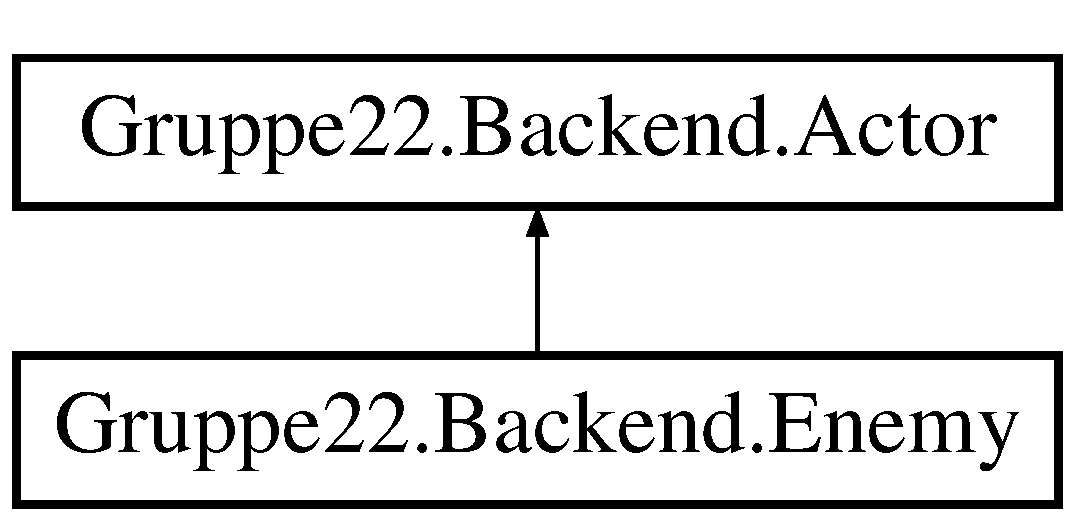
\includegraphics[height=2.000000cm]{class_gruppe22_1_1_backend_1_1_enemy}
\end{center}
\end{figure}
\subsection*{Öffentliche Methoden}
\begin{DoxyCompactItemize}
\item 
void \hyperlink{class_gruppe22_1_1_backend_1_1_enemy_a661dd6ecfdfcf03b4779883dcb0ab266}{Assign\-Skills\-And\-Abilities} ()
\item 
\hyperlink{class_gruppe22_1_1_backend_1_1_enemy_a9049d94b790aaabe76eeafaa5cfcdfcf}{Enemy} (Content\-Manager content, int \hyperlink{class_gruppe22_1_1_backend_1_1_actor_a46f3a7d62de83a6bf3c44cd52f38af9b}{health}=-\/1, int armour=-\/1, int \hyperlink{class_gruppe22_1_1_backend_1_1_actor_a461e2480a59de23517c3b375dede10fb}{damage}=-\/1, int \hyperlink{class_gruppe22_1_1_backend_1_1_actor_aac0f2f9a2f0b314f98ba19d0b38a7a97}{max\-Health}=-\/1, string \hyperlink{class_gruppe22_1_1_backend_1_1_actor_a28129eaf9d70d9bfc33a29544ba74edf}{name}=\char`\"{}\char`\"{}, Random r=null, int \hyperlink{class_gruppe22_1_1_backend_1_1_actor_aef8ca8637a54602399de1b2d08670c9e}{level}=1)
\begin{DoxyCompactList}\small\item\em Constructor \end{DoxyCompactList}\end{DoxyCompactItemize}
\subsection*{Weitere Geerbte Elemente}


\subsection{Beschreibung der Konstruktoren und Destruktoren}
\hypertarget{class_gruppe22_1_1_backend_1_1_enemy_a9049d94b790aaabe76eeafaa5cfcdfcf}{\index{Gruppe22\-::\-Backend\-::\-Enemy@{Gruppe22\-::\-Backend\-::\-Enemy}!Enemy@{Enemy}}
\index{Enemy@{Enemy}!Gruppe22::Backend::Enemy@{Gruppe22\-::\-Backend\-::\-Enemy}}
\subsubsection[{Enemy}]{\setlength{\rightskip}{0pt plus 5cm}Gruppe22.\-Backend.\-Enemy.\-Enemy (
\begin{DoxyParamCaption}
\item[{Content\-Manager}]{content, }
\item[{int}]{health = {\ttfamily -\/1}, }
\item[{int}]{armour = {\ttfamily -\/1}, }
\item[{int}]{damage = {\ttfamily -\/1}, }
\item[{int}]{max\-Health = {\ttfamily -\/1}, }
\item[{string}]{name = {\ttfamily \char`\"{}\char`\"{}}, }
\item[{Random}]{r = {\ttfamily null}, }
\item[{int}]{level = {\ttfamily 1}}
\end{DoxyParamCaption}
)}}\label{class_gruppe22_1_1_backend_1_1_enemy_a9049d94b790aaabe76eeafaa5cfcdfcf}


Constructor 



\subsection{Dokumentation der Elementfunktionen}
\hypertarget{class_gruppe22_1_1_backend_1_1_enemy_a661dd6ecfdfcf03b4779883dcb0ab266}{\index{Gruppe22\-::\-Backend\-::\-Enemy@{Gruppe22\-::\-Backend\-::\-Enemy}!Assign\-Skills\-And\-Abilities@{Assign\-Skills\-And\-Abilities}}
\index{Assign\-Skills\-And\-Abilities@{Assign\-Skills\-And\-Abilities}!Gruppe22::Backend::Enemy@{Gruppe22\-::\-Backend\-::\-Enemy}}
\subsubsection[{Assign\-Skills\-And\-Abilities}]{\setlength{\rightskip}{0pt plus 5cm}void Gruppe22.\-Backend.\-Enemy.\-Assign\-Skills\-And\-Abilities (
\begin{DoxyParamCaption}
{}
\end{DoxyParamCaption}
)}}\label{class_gruppe22_1_1_backend_1_1_enemy_a661dd6ecfdfcf03b4779883dcb0ab266}


Die Dokumentation für diese Klasse wurde erzeugt aufgrund der Datei\-:\begin{DoxyCompactItemize}
\item 
C\-:/\-Users/beursken/\-Documents/\-Git\-Hub/gruppe22/\-Gruppe22/\-Gruppe22/\-Backend/\-Actors/\hyperlink{_enemy_8cs}{Enemy.\-cs}\end{DoxyCompactItemize}

\hypertarget{class_gruppe22_1_1_backend_1_1_exit}{\section{Gruppe22.\-Backend.\-Exit Klassenreferenz}
\label{class_gruppe22_1_1_backend_1_1_exit}\index{Gruppe22.\-Backend.\-Exit@{Gruppe22.\-Backend.\-Exit}}
}
\subsection*{Öffentliche Methoden}
\begin{DoxyCompactItemize}
\item 
\hyperlink{class_gruppe22_1_1_backend_1_1_exit_a55274f1d0cdd8d6b01f1dd0187819885}{Exit} (\hyperlink{class_gruppe22_1_1_backend_1_1_coords}{Coords} \hyperlink{class_gruppe22_1_1_backend_1_1_exit_a1c66d12ccc76e3670276e5b6dff84432}{from}, string \hyperlink{class_gruppe22_1_1_backend_1_1_exit_a40c48584f9dcff97a7894b7f806fe602}{from\-Room}, \hyperlink{class_gruppe22_1_1_backend_1_1_coords}{Backend.\-Coords} \hyperlink{class_gruppe22_1_1_backend_1_1_exit_a4286116558464099383cae2dfaf75bf4}{to}=null, string \hyperlink{class_gruppe22_1_1_backend_1_1_exit_abbd47d66f499b32fa3824d1fdf14390d}{to\-Room}=\char`\"{}\char`\"{})
\end{DoxyCompactItemize}
\subsection*{Propertys}
\begin{DoxyCompactItemize}
\item 
\hyperlink{class_gruppe22_1_1_backend_1_1_coords}{Backend.\-Coords} \hyperlink{class_gruppe22_1_1_backend_1_1_exit_a1c66d12ccc76e3670276e5b6dff84432}{from}\hspace{0.3cm}{\ttfamily  \mbox{[}get\mbox{]}}
\item 
\hyperlink{class_gruppe22_1_1_backend_1_1_coords}{Backend.\-Coords} \hyperlink{class_gruppe22_1_1_backend_1_1_exit_a4286116558464099383cae2dfaf75bf4}{to}\hspace{0.3cm}{\ttfamily  \mbox{[}get\mbox{]}}
\item 
string \hyperlink{class_gruppe22_1_1_backend_1_1_exit_a40c48584f9dcff97a7894b7f806fe602}{from\-Room}\hspace{0.3cm}{\ttfamily  \mbox{[}get\mbox{]}}
\item 
string \hyperlink{class_gruppe22_1_1_backend_1_1_exit_abbd47d66f499b32fa3824d1fdf14390d}{to\-Room}\hspace{0.3cm}{\ttfamily  \mbox{[}get\mbox{]}}
\end{DoxyCompactItemize}


\subsection{Beschreibung der Konstruktoren und Destruktoren}
\hypertarget{class_gruppe22_1_1_backend_1_1_exit_a55274f1d0cdd8d6b01f1dd0187819885}{\index{Gruppe22\-::\-Backend\-::\-Exit@{Gruppe22\-::\-Backend\-::\-Exit}!Exit@{Exit}}
\index{Exit@{Exit}!Gruppe22::Backend::Exit@{Gruppe22\-::\-Backend\-::\-Exit}}
\subsubsection[{Exit}]{\setlength{\rightskip}{0pt plus 5cm}Gruppe22.\-Backend.\-Exit.\-Exit (
\begin{DoxyParamCaption}
\item[{{\bf Coords}}]{from, }
\item[{string}]{from\-Room, }
\item[{{\bf Backend.\-Coords}}]{to = {\ttfamily null}, }
\item[{string}]{to\-Room = {\ttfamily \char`\"{}\char`\"{}}}
\end{DoxyParamCaption}
)}}\label{class_gruppe22_1_1_backend_1_1_exit_a55274f1d0cdd8d6b01f1dd0187819885}


\subsection{Dokumentation der Propertys}
\hypertarget{class_gruppe22_1_1_backend_1_1_exit_a1c66d12ccc76e3670276e5b6dff84432}{\index{Gruppe22\-::\-Backend\-::\-Exit@{Gruppe22\-::\-Backend\-::\-Exit}!from@{from}}
\index{from@{from}!Gruppe22::Backend::Exit@{Gruppe22\-::\-Backend\-::\-Exit}}
\subsubsection[{from}]{\setlength{\rightskip}{0pt plus 5cm}{\bf Backend.\-Coords} Gruppe22.\-Backend.\-Exit.\-from\hspace{0.3cm}{\ttfamily [get]}}}\label{class_gruppe22_1_1_backend_1_1_exit_a1c66d12ccc76e3670276e5b6dff84432}
\hypertarget{class_gruppe22_1_1_backend_1_1_exit_a40c48584f9dcff97a7894b7f806fe602}{\index{Gruppe22\-::\-Backend\-::\-Exit@{Gruppe22\-::\-Backend\-::\-Exit}!from\-Room@{from\-Room}}
\index{from\-Room@{from\-Room}!Gruppe22::Backend::Exit@{Gruppe22\-::\-Backend\-::\-Exit}}
\subsubsection[{from\-Room}]{\setlength{\rightskip}{0pt plus 5cm}string Gruppe22.\-Backend.\-Exit.\-from\-Room\hspace{0.3cm}{\ttfamily [get]}}}\label{class_gruppe22_1_1_backend_1_1_exit_a40c48584f9dcff97a7894b7f806fe602}
\hypertarget{class_gruppe22_1_1_backend_1_1_exit_a4286116558464099383cae2dfaf75bf4}{\index{Gruppe22\-::\-Backend\-::\-Exit@{Gruppe22\-::\-Backend\-::\-Exit}!to@{to}}
\index{to@{to}!Gruppe22::Backend::Exit@{Gruppe22\-::\-Backend\-::\-Exit}}
\subsubsection[{to}]{\setlength{\rightskip}{0pt plus 5cm}{\bf Backend.\-Coords} Gruppe22.\-Backend.\-Exit.\-to\hspace{0.3cm}{\ttfamily [get]}}}\label{class_gruppe22_1_1_backend_1_1_exit_a4286116558464099383cae2dfaf75bf4}
\hypertarget{class_gruppe22_1_1_backend_1_1_exit_abbd47d66f499b32fa3824d1fdf14390d}{\index{Gruppe22\-::\-Backend\-::\-Exit@{Gruppe22\-::\-Backend\-::\-Exit}!to\-Room@{to\-Room}}
\index{to\-Room@{to\-Room}!Gruppe22::Backend::Exit@{Gruppe22\-::\-Backend\-::\-Exit}}
\subsubsection[{to\-Room}]{\setlength{\rightskip}{0pt plus 5cm}string Gruppe22.\-Backend.\-Exit.\-to\-Room\hspace{0.3cm}{\ttfamily [get]}}}\label{class_gruppe22_1_1_backend_1_1_exit_abbd47d66f499b32fa3824d1fdf14390d}


Die Dokumentation für diese Klasse wurde erzeugt aufgrund der Datei\-:\begin{DoxyCompactItemize}
\item 
C\-:/\-Users/beursken/\-Documents/\-Git\-Hub/gruppe22/\-Gruppe22/\-Gruppe22/\-Backend/\-Map/\hyperlink{_map_8cs}{Map.\-cs}\end{DoxyCompactItemize}

\hypertarget{class_gruppe22_1_1_client_1_1_file_dialog}{\section{Gruppe22.\-Client.\-File\-Dialog Klassenreferenz}
\label{class_gruppe22_1_1_client_1_1_file_dialog}\index{Gruppe22.\-Client.\-File\-Dialog@{Gruppe22.\-Client.\-File\-Dialog}}
}
Klassendiagramm für Gruppe22.\-Client.\-File\-Dialog\-:\begin{figure}[H]
\begin{center}
\leavevmode
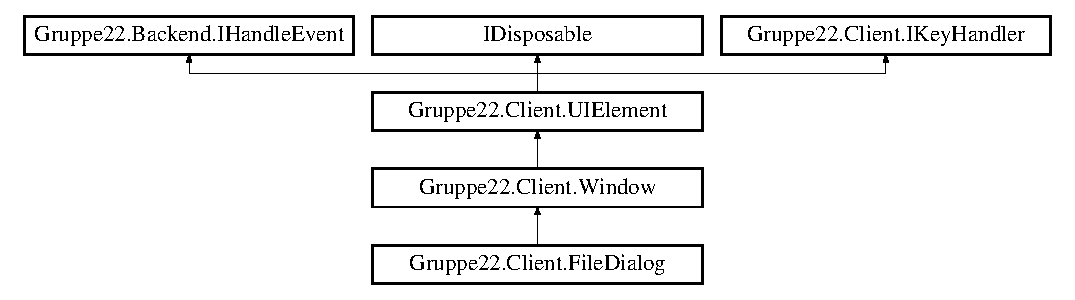
\includegraphics[height=3.589744cm]{class_gruppe22_1_1_client_1_1_file_dialog}
\end{center}
\end{figure}
\subsection*{Öffentliche Methoden}
\begin{DoxyCompactItemize}
\item 
\hyperlink{class_gruppe22_1_1_client_1_1_file_dialog_acb7d5884bb98286039801f4b5c1f852c}{File\-Dialog} (\hyperlink{interface_gruppe22_1_1_backend_1_1_i_handle_event}{Backend.\-I\-Handle\-Event} parent, Sprite\-Batch sprite\-Batch, Content\-Manager content, Rectangle display\-Rect)
\end{DoxyCompactItemize}
\subsection*{Weitere Geerbte Elemente}


\subsection{Beschreibung der Konstruktoren und Destruktoren}
\hypertarget{class_gruppe22_1_1_client_1_1_file_dialog_acb7d5884bb98286039801f4b5c1f852c}{\index{Gruppe22\-::\-Client\-::\-File\-Dialog@{Gruppe22\-::\-Client\-::\-File\-Dialog}!File\-Dialog@{File\-Dialog}}
\index{File\-Dialog@{File\-Dialog}!Gruppe22::Client::FileDialog@{Gruppe22\-::\-Client\-::\-File\-Dialog}}
\subsubsection[{File\-Dialog}]{\setlength{\rightskip}{0pt plus 5cm}Gruppe22.\-Client.\-File\-Dialog.\-File\-Dialog (
\begin{DoxyParamCaption}
\item[{{\bf Backend.\-I\-Handle\-Event}}]{parent, }
\item[{Sprite\-Batch}]{sprite\-Batch, }
\item[{Content\-Manager}]{content, }
\item[{Rectangle}]{display\-Rect}
\end{DoxyParamCaption}
)}}\label{class_gruppe22_1_1_client_1_1_file_dialog_acb7d5884bb98286039801f4b5c1f852c}


Die Dokumentation für diese Klasse wurde erzeugt aufgrund der Datei\-:\begin{DoxyCompactItemize}
\item 
C\-:/\-Users/beursken/\-Documents/\-Git\-Hub/gruppe22/\-Gruppe22/\-Gruppe22/\-Client/\-U\-I/\hyperlink{_file_dialog_8cs}{File\-Dialog.\-cs}\end{DoxyCompactItemize}

\hypertarget{class_gruppe22_1_1_client_1_1_float_number}{\section{Gruppe22.\-Client.\-Float\-Number Klassenreferenz}
\label{class_gruppe22_1_1_client_1_1_float_number}\index{Gruppe22.\-Client.\-Float\-Number@{Gruppe22.\-Client.\-Float\-Number}}
}
\subsection*{Öffentliche Methoden}
\begin{DoxyCompactItemize}
\item 
void \hyperlink{class_gruppe22_1_1_client_1_1_float_number_aac25fa8a3ace459211a9e2f5fe6e553d}{Draw} ()
\item 
bool \hyperlink{class_gruppe22_1_1_client_1_1_float_number_a09188feffb25fcfc7aab55ad04e90463}{Update} (Game\-Time gametime)
\item 
\hyperlink{class_gruppe22_1_1_client_1_1_float_number_a7d94ecc2b6192c12272c3587b1e72aaf}{Float\-Number} (Content\-Manager content, Sprite\-Batch batch, \hyperlink{class_gruppe22_1_1_backend_1_1_coords}{Backend.\-Coords} coords, string text, \hyperlink{class_gruppe22_1_1_client_1_1_camera}{Camera} camera, Color color, int counter=10, uint \hyperlink{class_gruppe22_1_1_client_1_1_float_number_a631929f5625e5c39b4924da3f57b684f}{delay}=0)
\item 
\hyperlink{class_gruppe22_1_1_client_1_1_float_number_a1e2b224422c410ec2b94ea5b3f9c26fe}{Float\-Number} (Content\-Manager content, Sprite\-Batch batch, \hyperlink{class_gruppe22_1_1_backend_1_1_coords}{Backend.\-Coords} coords, string text, \hyperlink{class_gruppe22_1_1_client_1_1_camera}{Camera} camera)
\end{DoxyCompactItemize}
\subsection*{Propertys}
\begin{DoxyCompactItemize}
\item 
uint \hyperlink{class_gruppe22_1_1_client_1_1_float_number_a631929f5625e5c39b4924da3f57b684f}{delay}\hspace{0.3cm}{\ttfamily  \mbox{[}get, set\mbox{]}}
\end{DoxyCompactItemize}


\subsection{Beschreibung der Konstruktoren und Destruktoren}
\hypertarget{class_gruppe22_1_1_client_1_1_float_number_a7d94ecc2b6192c12272c3587b1e72aaf}{\index{Gruppe22\-::\-Client\-::\-Float\-Number@{Gruppe22\-::\-Client\-::\-Float\-Number}!Float\-Number@{Float\-Number}}
\index{Float\-Number@{Float\-Number}!Gruppe22::Client::FloatNumber@{Gruppe22\-::\-Client\-::\-Float\-Number}}
\subsubsection[{Float\-Number}]{\setlength{\rightskip}{0pt plus 5cm}Gruppe22.\-Client.\-Float\-Number.\-Float\-Number (
\begin{DoxyParamCaption}
\item[{Content\-Manager}]{content, }
\item[{Sprite\-Batch}]{batch, }
\item[{{\bf Backend.\-Coords}}]{coords, }
\item[{string}]{text, }
\item[{{\bf Camera}}]{camera, }
\item[{Color}]{color, }
\item[{int}]{counter = {\ttfamily 10}, }
\item[{uint}]{delay = {\ttfamily 0}}
\end{DoxyParamCaption}
)}}\label{class_gruppe22_1_1_client_1_1_float_number_a7d94ecc2b6192c12272c3587b1e72aaf}
\hypertarget{class_gruppe22_1_1_client_1_1_float_number_a1e2b224422c410ec2b94ea5b3f9c26fe}{\index{Gruppe22\-::\-Client\-::\-Float\-Number@{Gruppe22\-::\-Client\-::\-Float\-Number}!Float\-Number@{Float\-Number}}
\index{Float\-Number@{Float\-Number}!Gruppe22::Client::FloatNumber@{Gruppe22\-::\-Client\-::\-Float\-Number}}
\subsubsection[{Float\-Number}]{\setlength{\rightskip}{0pt plus 5cm}Gruppe22.\-Client.\-Float\-Number.\-Float\-Number (
\begin{DoxyParamCaption}
\item[{Content\-Manager}]{content, }
\item[{Sprite\-Batch}]{batch, }
\item[{{\bf Backend.\-Coords}}]{coords, }
\item[{string}]{text, }
\item[{{\bf Camera}}]{camera}
\end{DoxyParamCaption}
)}}\label{class_gruppe22_1_1_client_1_1_float_number_a1e2b224422c410ec2b94ea5b3f9c26fe}


\subsection{Dokumentation der Elementfunktionen}
\hypertarget{class_gruppe22_1_1_client_1_1_float_number_aac25fa8a3ace459211a9e2f5fe6e553d}{\index{Gruppe22\-::\-Client\-::\-Float\-Number@{Gruppe22\-::\-Client\-::\-Float\-Number}!Draw@{Draw}}
\index{Draw@{Draw}!Gruppe22::Client::FloatNumber@{Gruppe22\-::\-Client\-::\-Float\-Number}}
\subsubsection[{Draw}]{\setlength{\rightskip}{0pt plus 5cm}void Gruppe22.\-Client.\-Float\-Number.\-Draw (
\begin{DoxyParamCaption}
{}
\end{DoxyParamCaption}
)}}\label{class_gruppe22_1_1_client_1_1_float_number_aac25fa8a3ace459211a9e2f5fe6e553d}
\hypertarget{class_gruppe22_1_1_client_1_1_float_number_a09188feffb25fcfc7aab55ad04e90463}{\index{Gruppe22\-::\-Client\-::\-Float\-Number@{Gruppe22\-::\-Client\-::\-Float\-Number}!Update@{Update}}
\index{Update@{Update}!Gruppe22::Client::FloatNumber@{Gruppe22\-::\-Client\-::\-Float\-Number}}
\subsubsection[{Update}]{\setlength{\rightskip}{0pt plus 5cm}bool Gruppe22.\-Client.\-Float\-Number.\-Update (
\begin{DoxyParamCaption}
\item[{Game\-Time}]{gametime}
\end{DoxyParamCaption}
)}}\label{class_gruppe22_1_1_client_1_1_float_number_a09188feffb25fcfc7aab55ad04e90463}


\subsection{Dokumentation der Propertys}
\hypertarget{class_gruppe22_1_1_client_1_1_float_number_a631929f5625e5c39b4924da3f57b684f}{\index{Gruppe22\-::\-Client\-::\-Float\-Number@{Gruppe22\-::\-Client\-::\-Float\-Number}!delay@{delay}}
\index{delay@{delay}!Gruppe22::Client::FloatNumber@{Gruppe22\-::\-Client\-::\-Float\-Number}}
\subsubsection[{delay}]{\setlength{\rightskip}{0pt plus 5cm}uint Gruppe22.\-Client.\-Float\-Number.\-delay\hspace{0.3cm}{\ttfamily [get]}, {\ttfamily [set]}}}\label{class_gruppe22_1_1_client_1_1_float_number_a631929f5625e5c39b4924da3f57b684f}


Die Dokumentation für diese Klasse wurde erzeugt aufgrund der Datei\-:\begin{DoxyCompactItemize}
\item 
C\-:/\-Users/beursken/\-Documents/\-Git\-Hub/gruppe22/\-Gruppe22/\-Gruppe22/\-Client/\-Map/\hyperlink{_mainmap_8cs}{Mainmap.\-cs}\end{DoxyCompactItemize}

\hypertarget{class_gruppe22_1_1_backend_1_1_floor_tile}{\section{Gruppe22.\-Backend.\-Floor\-Tile Klassenreferenz}
\label{class_gruppe22_1_1_backend_1_1_floor_tile}\index{Gruppe22.\-Backend.\-Floor\-Tile@{Gruppe22.\-Backend.\-Floor\-Tile}}
}
Klassendiagramm für Gruppe22.\-Backend.\-Floor\-Tile\-:\begin{figure}[H]
\begin{center}
\leavevmode
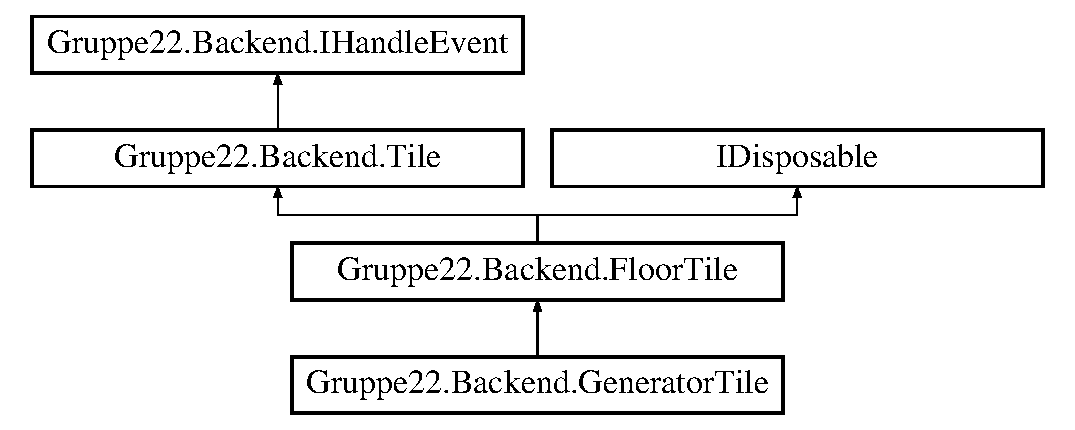
\includegraphics[height=4.000000cm]{class_gruppe22_1_1_backend_1_1_floor_tile}
\end{center}
\end{figure}
\subsection*{Öffentliche Methoden}
\begin{DoxyCompactItemize}
\item 
override void \hyperlink{class_gruppe22_1_1_backend_1_1_floor_tile_ae3d0627204d49dabc8180fd0bdd22803}{Update} (Game\-Time game\-Time)
\begin{DoxyCompactList}\small\item\em Refresh tiles which do something (traps, enemies, N\-P\-Cs) \end{DoxyCompactList}\item 
void \hyperlink{class_gruppe22_1_1_backend_1_1_floor_tile_aa181d883ef238dfca1615db12ab80606}{Remove} (\hyperlink{namespace_gruppe22_1_1_backend_a5956dac270a0deefca1d578d210550e2}{Tile\-Type} type)
\begin{DoxyCompactList}\small\item\em Remove all tiles of a specified type from overlay \end{DoxyCompactList}\item 
void \hyperlink{class_gruppe22_1_1_backend_1_1_floor_tile_a153d21fb6b8e240d822370e0c20d6ce5}{Add} (\hyperlink{class_gruppe22_1_1_backend_1_1_tile}{Tile} tile, bool update=false)
\begin{DoxyCompactList}\small\item\em Add specified tile to overlay \end{DoxyCompactList}\item 
void \hyperlink{class_gruppe22_1_1_backend_1_1_floor_tile_a6533275079b634b5fadc5cd0d1ba927f}{Remove} (\hyperlink{class_gruppe22_1_1_backend_1_1_tile}{Tile} tile)
\begin{DoxyCompactList}\small\item\em Remove specified tile from overlay \end{DoxyCompactList}\item 
\hyperlink{class_gruppe22_1_1_backend_1_1_floor_tile_a828c82cc335a8c8416861a11b0d70f65}{Floor\-Tile} (object \hyperlink{class_gruppe22_1_1_backend_1_1_tile_abc12933c70eb3a2ebbb2fde9f45c2632}{parent})
\begin{DoxyCompactList}\small\item\em A empty constructor \end{DoxyCompactList}\item 
\hyperlink{class_gruppe22_1_1_backend_1_1_floor_tile_ae90ab35dfdebf892a27d545d1fef32c0}{Floor\-Tile} (object \hyperlink{class_gruppe22_1_1_backend_1_1_tile_abc12933c70eb3a2ebbb2fde9f45c2632}{parent}, \hyperlink{class_gruppe22_1_1_backend_1_1_coords}{Backend.\-Coords} \hyperlink{class_gruppe22_1_1_backend_1_1_floor_tile_a222af0c5d8ea6b7d24d04a384f71d70b}{coords}=null, bool \hyperlink{class_gruppe22_1_1_backend_1_1_floor_tile_a07516e27f9669dd9e852cf42a1a94635}{can\-Enter}=true)
\begin{DoxyCompactList}\small\item\em A constructor adding a walltile to the overlay if the contructed tile is impassable \end{DoxyCompactList}\item 
override void \hyperlink{class_gruppe22_1_1_backend_1_1_floor_tile_a4a096b8d6ff25557bd807751268987f2}{Save} (Xml\-Writer xmlw)
\begin{DoxyCompactList}\small\item\em Save the Floortile and every tile in it's overlay \end{DoxyCompactList}\item 
void \hyperlink{class_gruppe22_1_1_backend_1_1_floor_tile_a37dbc28f0467127f30aaddf709975c70}{Dispose} ()
\begin{DoxyCompactList}\small\item\em Clean up \hyperlink{class_gruppe22_1_1_backend_1_1_tile}{Tile} \end{DoxyCompactList}\end{DoxyCompactItemize}
\subsection*{Geschützte Attribute}
\begin{DoxyCompactItemize}
\item 
List$<$ \hyperlink{class_gruppe22_1_1_backend_1_1_tile}{Tile} $>$ \hyperlink{class_gruppe22_1_1_backend_1_1_floor_tile_ac860f59975d901d76d45681acf9d61f4}{\-\_\-overlay}
\begin{DoxyCompactList}\small\item\em Fields displayed (and checked) on top of the current field \end{DoxyCompactList}\item 
\hyperlink{class_gruppe22_1_1_backend_1_1_coords}{Backend.\-Coords} \hyperlink{class_gruppe22_1_1_backend_1_1_floor_tile_a192eaa6b557b27ddebe7a16ea38d13e5}{\-\_\-coords} = null
\begin{DoxyCompactList}\small\item\em The Position of the tile \end{DoxyCompactList}\end{DoxyCompactItemize}
\subsection*{Propertys}
\begin{DoxyCompactItemize}
\item 
List$<$ \hyperlink{class_gruppe22_1_1_backend_1_1_tile}{Tile} $>$ \hyperlink{class_gruppe22_1_1_backend_1_1_floor_tile_a8ce0005a15cfaf89ec382a84ef908c8f}{overlay}\hspace{0.3cm}{\ttfamily  \mbox{[}get, set\mbox{]}}
\item 
List$<$ \hyperlink{class_gruppe22_1_1_backend_1_1_actor}{Actor} $>$ \hyperlink{class_gruppe22_1_1_backend_1_1_floor_tile_a7e345b719614f87d9473c10afe55cb61}{actors}\hspace{0.3cm}{\ttfamily  \mbox{[}get\mbox{]}}
\item 
List$<$ \hyperlink{class_gruppe22_1_1_backend_1_1_item}{Item} $>$ \hyperlink{class_gruppe22_1_1_backend_1_1_floor_tile_a9ffbcbcaade0609f83172fa271e33563}{items}\hspace{0.3cm}{\ttfamily  \mbox{[}get\mbox{]}}
\item 
\hyperlink{class_gruppe22_1_1_backend_1_1_trap_tile}{Trap\-Tile} \hyperlink{class_gruppe22_1_1_backend_1_1_floor_tile_a1f5554db761650899c2fdd571ceff000}{trap}\hspace{0.3cm}{\ttfamily  \mbox{[}get\mbox{]}}
\item 
\hyperlink{class_gruppe22_1_1_backend_1_1_checkpoint_tile}{Checkpoint\-Tile} \hyperlink{class_gruppe22_1_1_backend_1_1_floor_tile_a1a86ae2cd1bcf068a31649d51c5bb49a}{checkpoint}\hspace{0.3cm}{\ttfamily  \mbox{[}get\mbox{]}}
\item 
\hyperlink{class_gruppe22_1_1_backend_1_1_teleport_tile}{Teleport\-Tile} \hyperlink{class_gruppe22_1_1_backend_1_1_floor_tile_a9276aed0713002718a978669f237b106}{teleport}\hspace{0.3cm}{\ttfamily  \mbox{[}get\mbox{]}}
\item 
\hyperlink{class_gruppe22_1_1_backend_1_1_actor}{Actor} \hyperlink{class_gruppe22_1_1_backend_1_1_floor_tile_ae61e1f6a710ca100e86c94f6150b233e}{first\-Actor}\hspace{0.3cm}{\ttfamily  \mbox{[}get\mbox{]}}
\item 
\hyperlink{class_gruppe22_1_1_backend_1_1_reserved_tile}{Reserved\-Tile} \hyperlink{class_gruppe22_1_1_backend_1_1_floor_tile_a8929f5ce72b9deb76b2babb69e08c308}{reserved}\hspace{0.3cm}{\ttfamily  \mbox{[}get\mbox{]}}
\item 
\hyperlink{class_gruppe22_1_1_backend_1_1_door_tile}{Door\-Tile} \hyperlink{class_gruppe22_1_1_backend_1_1_floor_tile_a42b9b51aaeb0118ee2cc1ae5f0d4d29f}{door}\hspace{0.3cm}{\ttfamily  \mbox{[}get\mbox{]}}
\item 
\hyperlink{class_gruppe22_1_1_backend_1_1_item_tile}{Item\-Tile} \hyperlink{class_gruppe22_1_1_backend_1_1_floor_tile_af1b9c44771c17dd815b3386d66a09329}{first\-Item}\hspace{0.3cm}{\ttfamily  \mbox{[}get\mbox{]}}
\item 
new \hyperlink{class_gruppe22_1_1_backend_1_1_coords}{Backend.\-Coords} \hyperlink{class_gruppe22_1_1_backend_1_1_floor_tile_a222af0c5d8ea6b7d24d04a384f71d70b}{coords}\hspace{0.3cm}{\ttfamily  \mbox{[}get, set\mbox{]}}
\item 
bool \hyperlink{class_gruppe22_1_1_backend_1_1_floor_tile_a4dc2e696b9103c702ebbf5a8f898f99d}{has\-Checkpoint}\hspace{0.3cm}{\ttfamily  \mbox{[}get\mbox{]}}
\begin{DoxyCompactList}\small\item\em Determine whether tile has a checkpoint on it \end{DoxyCompactList}\item 
bool \hyperlink{class_gruppe22_1_1_backend_1_1_floor_tile_a07516e27f9669dd9e852cf42a1a94635}{can\-Enter}\hspace{0.3cm}{\ttfamily  \mbox{[}get\mbox{]}}
\begin{DoxyCompactList}\small\item\em Determine whether tile can be entered \end{DoxyCompactList}\item 
bool \hyperlink{class_gruppe22_1_1_backend_1_1_floor_tile_ad5e7dcc45afdb6acf6eca5510ae38049}{has\-Wall}\hspace{0.3cm}{\ttfamily  \mbox{[}get\mbox{]}}
\begin{DoxyCompactList}\small\item\em Determine whether tile has a wall on it \end{DoxyCompactList}\item 
\hyperlink{namespace_gruppe22_1_1_backend_ab19de7e2856537f39fbd380beea6ddba}{Wall\-Type} \hyperlink{class_gruppe22_1_1_backend_1_1_floor_tile_af235974bebb657c12a310521c1e8293d}{wall\-Type}\hspace{0.3cm}{\ttfamily  \mbox{[}get\mbox{]}}
\item 
bool \hyperlink{class_gruppe22_1_1_backend_1_1_floor_tile_ab92743f9c2bebd18192a91d7a1c2c194}{has\-Door}\hspace{0.3cm}{\ttfamily  \mbox{[}get\mbox{]}}
\begin{DoxyCompactList}\small\item\em Determine whether tile has a door on it \end{DoxyCompactList}\item 
int \hyperlink{class_gruppe22_1_1_backend_1_1_floor_tile_aba100c4046831211768aeddb2851f6b2}{floor\-Style}\hspace{0.3cm}{\ttfamily  \mbox{[}get\mbox{]}}
\begin{DoxyCompactList}\small\item\em Determine whether tile has a special floor style (empty space, fire, water, road, grass, rocks, etc.) \end{DoxyCompactList}\item 
bool \hyperlink{class_gruppe22_1_1_backend_1_1_floor_tile_a13d1616f29393cef6bebe40c140902e2}{has\-Player}\hspace{0.3cm}{\ttfamily  \mbox{[}get\mbox{]}}
\begin{DoxyCompactList}\small\item\em Determine whether a player is standing on the current tile \end{DoxyCompactList}\item 
bool \hyperlink{class_gruppe22_1_1_backend_1_1_floor_tile_a48a520d5f87a7f53f967d332458137b2}{has\-N\-P\-C}\hspace{0.3cm}{\ttfamily  \mbox{[}get\mbox{]}}
\begin{DoxyCompactList}\small\item\em Determine whether an enemy is standing on the current tile \end{DoxyCompactList}\item 
bool \hyperlink{class_gruppe22_1_1_backend_1_1_floor_tile_afe86d0c8424017818f04e2b0688e5c75}{has\-Enemy}\hspace{0.3cm}{\ttfamily  \mbox{[}get\mbox{]}}
\begin{DoxyCompactList}\small\item\em Determine whether an enemy is standing on the current tile \end{DoxyCompactList}\item 
bool \hyperlink{class_gruppe22_1_1_backend_1_1_floor_tile_a477120ecb285df256f1761cd1774bf16}{has\-Teleport}\hspace{0.3cm}{\ttfamily  \mbox{[}get\mbox{]}}
\begin{DoxyCompactList}\small\item\em Determine whether the current tile contains a teleporter \end{DoxyCompactList}\item 
bool \hyperlink{class_gruppe22_1_1_backend_1_1_floor_tile_a6d2ae9e7cbc9de3a2c39ddd0fbf2cee6}{has\-Trap}\hspace{0.3cm}{\ttfamily  \mbox{[}get\mbox{]}}
\begin{DoxyCompactList}\small\item\em Determine whether the current tile has a trap on it \end{DoxyCompactList}\item 
bool \hyperlink{class_gruppe22_1_1_backend_1_1_floor_tile_aa62f725bbf60ab19f680d56bef8d7848}{has\-Treasure}\hspace{0.3cm}{\ttfamily  \mbox{[}get\mbox{]}}
\begin{DoxyCompactList}\small\item\em Determine whether there is a treasure on the current tile \end{DoxyCompactList}\item 
bool \hyperlink{class_gruppe22_1_1_backend_1_1_floor_tile_a285da5ca4d7d6a6af58fff71c1156a91}{visible}\hspace{0.3cm}{\ttfamily  \mbox{[}get, set\mbox{]}}
\item 
bool \hyperlink{class_gruppe22_1_1_backend_1_1_floor_tile_af31534372c3138a5e67ce531adead203}{has\-Target}\hspace{0.3cm}{\ttfamily  \mbox{[}get\mbox{]}}
\begin{DoxyCompactList}\small\item\em Determine whether the current tile is the 'end' of the game \end{DoxyCompactList}\end{DoxyCompactItemize}


\subsection{Beschreibung der Konstruktoren und Destruktoren}
\hypertarget{class_gruppe22_1_1_backend_1_1_floor_tile_a828c82cc335a8c8416861a11b0d70f65}{\index{Gruppe22\-::\-Backend\-::\-Floor\-Tile@{Gruppe22\-::\-Backend\-::\-Floor\-Tile}!Floor\-Tile@{Floor\-Tile}}
\index{Floor\-Tile@{Floor\-Tile}!Gruppe22::Backend::FloorTile@{Gruppe22\-::\-Backend\-::\-Floor\-Tile}}
\subsubsection[{Floor\-Tile}]{\setlength{\rightskip}{0pt plus 5cm}Gruppe22.\-Backend.\-Floor\-Tile.\-Floor\-Tile (
\begin{DoxyParamCaption}
\item[{object}]{parent}
\end{DoxyParamCaption}
)}}\label{class_gruppe22_1_1_backend_1_1_floor_tile_a828c82cc335a8c8416861a11b0d70f65}


A empty constructor 

\hypertarget{class_gruppe22_1_1_backend_1_1_floor_tile_ae90ab35dfdebf892a27d545d1fef32c0}{\index{Gruppe22\-::\-Backend\-::\-Floor\-Tile@{Gruppe22\-::\-Backend\-::\-Floor\-Tile}!Floor\-Tile@{Floor\-Tile}}
\index{Floor\-Tile@{Floor\-Tile}!Gruppe22::Backend::FloorTile@{Gruppe22\-::\-Backend\-::\-Floor\-Tile}}
\subsubsection[{Floor\-Tile}]{\setlength{\rightskip}{0pt plus 5cm}Gruppe22.\-Backend.\-Floor\-Tile.\-Floor\-Tile (
\begin{DoxyParamCaption}
\item[{object}]{parent, }
\item[{{\bf Backend.\-Coords}}]{coords = {\ttfamily null}, }
\item[{bool}]{can\-Enter = {\ttfamily true}}
\end{DoxyParamCaption}
)}}\label{class_gruppe22_1_1_backend_1_1_floor_tile_ae90ab35dfdebf892a27d545d1fef32c0}


A constructor adding a walltile to the overlay if the contructed tile is impassable 



\subsection{Dokumentation der Elementfunktionen}
\hypertarget{class_gruppe22_1_1_backend_1_1_floor_tile_a153d21fb6b8e240d822370e0c20d6ce5}{\index{Gruppe22\-::\-Backend\-::\-Floor\-Tile@{Gruppe22\-::\-Backend\-::\-Floor\-Tile}!Add@{Add}}
\index{Add@{Add}!Gruppe22::Backend::FloorTile@{Gruppe22\-::\-Backend\-::\-Floor\-Tile}}
\subsubsection[{Add}]{\setlength{\rightskip}{0pt plus 5cm}void Gruppe22.\-Backend.\-Floor\-Tile.\-Add (
\begin{DoxyParamCaption}
\item[{{\bf Tile}}]{tile, }
\item[{bool}]{update = {\ttfamily false}}
\end{DoxyParamCaption}
)}}\label{class_gruppe22_1_1_backend_1_1_floor_tile_a153d21fb6b8e240d822370e0c20d6ce5}


Add specified tile to overlay 


\begin{DoxyParams}{Parameter}
{\em tile} & \\
\hline
\end{DoxyParams}
\hypertarget{class_gruppe22_1_1_backend_1_1_floor_tile_a37dbc28f0467127f30aaddf709975c70}{\index{Gruppe22\-::\-Backend\-::\-Floor\-Tile@{Gruppe22\-::\-Backend\-::\-Floor\-Tile}!Dispose@{Dispose}}
\index{Dispose@{Dispose}!Gruppe22::Backend::FloorTile@{Gruppe22\-::\-Backend\-::\-Floor\-Tile}}
\subsubsection[{Dispose}]{\setlength{\rightskip}{0pt plus 5cm}void Gruppe22.\-Backend.\-Floor\-Tile.\-Dispose (
\begin{DoxyParamCaption}
{}
\end{DoxyParamCaption}
)}}\label{class_gruppe22_1_1_backend_1_1_floor_tile_a37dbc28f0467127f30aaddf709975c70}


Clean up \hyperlink{class_gruppe22_1_1_backend_1_1_tile}{Tile} 

\hypertarget{class_gruppe22_1_1_backend_1_1_floor_tile_aa181d883ef238dfca1615db12ab80606}{\index{Gruppe22\-::\-Backend\-::\-Floor\-Tile@{Gruppe22\-::\-Backend\-::\-Floor\-Tile}!Remove@{Remove}}
\index{Remove@{Remove}!Gruppe22::Backend::FloorTile@{Gruppe22\-::\-Backend\-::\-Floor\-Tile}}
\subsubsection[{Remove}]{\setlength{\rightskip}{0pt plus 5cm}void Gruppe22.\-Backend.\-Floor\-Tile.\-Remove (
\begin{DoxyParamCaption}
\item[{{\bf Tile\-Type}}]{type}
\end{DoxyParamCaption}
)}}\label{class_gruppe22_1_1_backend_1_1_floor_tile_aa181d883ef238dfca1615db12ab80606}


Remove all tiles of a specified type from overlay 


\begin{DoxyParams}{Parameter}
{\em type} & \\
\hline
\end{DoxyParams}
\hypertarget{class_gruppe22_1_1_backend_1_1_floor_tile_a6533275079b634b5fadc5cd0d1ba927f}{\index{Gruppe22\-::\-Backend\-::\-Floor\-Tile@{Gruppe22\-::\-Backend\-::\-Floor\-Tile}!Remove@{Remove}}
\index{Remove@{Remove}!Gruppe22::Backend::FloorTile@{Gruppe22\-::\-Backend\-::\-Floor\-Tile}}
\subsubsection[{Remove}]{\setlength{\rightskip}{0pt plus 5cm}void Gruppe22.\-Backend.\-Floor\-Tile.\-Remove (
\begin{DoxyParamCaption}
\item[{{\bf Tile}}]{tile}
\end{DoxyParamCaption}
)}}\label{class_gruppe22_1_1_backend_1_1_floor_tile_a6533275079b634b5fadc5cd0d1ba927f}


Remove specified tile from overlay 


\begin{DoxyParams}{Parameter}
{\em tile} & \\
\hline
\end{DoxyParams}
\hypertarget{class_gruppe22_1_1_backend_1_1_floor_tile_a4a096b8d6ff25557bd807751268987f2}{\index{Gruppe22\-::\-Backend\-::\-Floor\-Tile@{Gruppe22\-::\-Backend\-::\-Floor\-Tile}!Save@{Save}}
\index{Save@{Save}!Gruppe22::Backend::FloorTile@{Gruppe22\-::\-Backend\-::\-Floor\-Tile}}
\subsubsection[{Save}]{\setlength{\rightskip}{0pt plus 5cm}override void Gruppe22.\-Backend.\-Floor\-Tile.\-Save (
\begin{DoxyParamCaption}
\item[{Xml\-Writer}]{xmlw}
\end{DoxyParamCaption}
)\hspace{0.3cm}{\ttfamily [virtual]}}}\label{class_gruppe22_1_1_backend_1_1_floor_tile_a4a096b8d6ff25557bd807751268987f2}


Save the Floortile and every tile in it's overlay 



Erneute Implementation von \hyperlink{class_gruppe22_1_1_backend_1_1_tile_a109ab3e77ffca9d44c95a711af3491dc}{Gruppe22.\-Backend.\-Tile}.

\hypertarget{class_gruppe22_1_1_backend_1_1_floor_tile_ae3d0627204d49dabc8180fd0bdd22803}{\index{Gruppe22\-::\-Backend\-::\-Floor\-Tile@{Gruppe22\-::\-Backend\-::\-Floor\-Tile}!Update@{Update}}
\index{Update@{Update}!Gruppe22::Backend::FloorTile@{Gruppe22\-::\-Backend\-::\-Floor\-Tile}}
\subsubsection[{Update}]{\setlength{\rightskip}{0pt plus 5cm}override void Gruppe22.\-Backend.\-Floor\-Tile.\-Update (
\begin{DoxyParamCaption}
\item[{Game\-Time}]{game\-Time}
\end{DoxyParamCaption}
)\hspace{0.3cm}{\ttfamily [virtual]}}}\label{class_gruppe22_1_1_backend_1_1_floor_tile_ae3d0627204d49dabc8180fd0bdd22803}


Refresh tiles which do something (traps, enemies, N\-P\-Cs) 


\begin{DoxyParams}{Parameter}
{\em game\-Time} & \\
\hline
\end{DoxyParams}


Erneute Implementation von \hyperlink{class_gruppe22_1_1_backend_1_1_tile_a0810154a52f859e852497e3717998e47}{Gruppe22.\-Backend.\-Tile}.



\subsection{Dokumentation der Datenelemente}
\hypertarget{class_gruppe22_1_1_backend_1_1_floor_tile_a192eaa6b557b27ddebe7a16ea38d13e5}{\index{Gruppe22\-::\-Backend\-::\-Floor\-Tile@{Gruppe22\-::\-Backend\-::\-Floor\-Tile}!\-\_\-coords@{\-\_\-coords}}
\index{\-\_\-coords@{\-\_\-coords}!Gruppe22::Backend::FloorTile@{Gruppe22\-::\-Backend\-::\-Floor\-Tile}}
\subsubsection[{\-\_\-coords}]{\setlength{\rightskip}{0pt plus 5cm}{\bf Backend.\-Coords} Gruppe22.\-Backend.\-Floor\-Tile.\-\_\-coords = null\hspace{0.3cm}{\ttfamily [protected]}}}\label{class_gruppe22_1_1_backend_1_1_floor_tile_a192eaa6b557b27ddebe7a16ea38d13e5}


The Position of the tile 

\hypertarget{class_gruppe22_1_1_backend_1_1_floor_tile_ac860f59975d901d76d45681acf9d61f4}{\index{Gruppe22\-::\-Backend\-::\-Floor\-Tile@{Gruppe22\-::\-Backend\-::\-Floor\-Tile}!\-\_\-overlay@{\-\_\-overlay}}
\index{\-\_\-overlay@{\-\_\-overlay}!Gruppe22::Backend::FloorTile@{Gruppe22\-::\-Backend\-::\-Floor\-Tile}}
\subsubsection[{\-\_\-overlay}]{\setlength{\rightskip}{0pt plus 5cm}List$<${\bf Tile}$>$ Gruppe22.\-Backend.\-Floor\-Tile.\-\_\-overlay\hspace{0.3cm}{\ttfamily [protected]}}}\label{class_gruppe22_1_1_backend_1_1_floor_tile_ac860f59975d901d76d45681acf9d61f4}


Fields displayed (and checked) on top of the current field 



\subsection{Dokumentation der Propertys}
\hypertarget{class_gruppe22_1_1_backend_1_1_floor_tile_a7e345b719614f87d9473c10afe55cb61}{\index{Gruppe22\-::\-Backend\-::\-Floor\-Tile@{Gruppe22\-::\-Backend\-::\-Floor\-Tile}!actors@{actors}}
\index{actors@{actors}!Gruppe22::Backend::FloorTile@{Gruppe22\-::\-Backend\-::\-Floor\-Tile}}
\subsubsection[{actors}]{\setlength{\rightskip}{0pt plus 5cm}List$<${\bf Actor}$>$ Gruppe22.\-Backend.\-Floor\-Tile.\-actors\hspace{0.3cm}{\ttfamily [get]}}}\label{class_gruppe22_1_1_backend_1_1_floor_tile_a7e345b719614f87d9473c10afe55cb61}
\hypertarget{class_gruppe22_1_1_backend_1_1_floor_tile_a07516e27f9669dd9e852cf42a1a94635}{\index{Gruppe22\-::\-Backend\-::\-Floor\-Tile@{Gruppe22\-::\-Backend\-::\-Floor\-Tile}!can\-Enter@{can\-Enter}}
\index{can\-Enter@{can\-Enter}!Gruppe22::Backend::FloorTile@{Gruppe22\-::\-Backend\-::\-Floor\-Tile}}
\subsubsection[{can\-Enter}]{\setlength{\rightskip}{0pt plus 5cm}bool Gruppe22.\-Backend.\-Floor\-Tile.\-can\-Enter\hspace{0.3cm}{\ttfamily [get]}}}\label{class_gruppe22_1_1_backend_1_1_floor_tile_a07516e27f9669dd9e852cf42a1a94635}


Determine whether tile can be entered 

\hypertarget{class_gruppe22_1_1_backend_1_1_floor_tile_a1a86ae2cd1bcf068a31649d51c5bb49a}{\index{Gruppe22\-::\-Backend\-::\-Floor\-Tile@{Gruppe22\-::\-Backend\-::\-Floor\-Tile}!checkpoint@{checkpoint}}
\index{checkpoint@{checkpoint}!Gruppe22::Backend::FloorTile@{Gruppe22\-::\-Backend\-::\-Floor\-Tile}}
\subsubsection[{checkpoint}]{\setlength{\rightskip}{0pt plus 5cm}{\bf Checkpoint\-Tile} Gruppe22.\-Backend.\-Floor\-Tile.\-checkpoint\hspace{0.3cm}{\ttfamily [get]}}}\label{class_gruppe22_1_1_backend_1_1_floor_tile_a1a86ae2cd1bcf068a31649d51c5bb49a}
\hypertarget{class_gruppe22_1_1_backend_1_1_floor_tile_a222af0c5d8ea6b7d24d04a384f71d70b}{\index{Gruppe22\-::\-Backend\-::\-Floor\-Tile@{Gruppe22\-::\-Backend\-::\-Floor\-Tile}!coords@{coords}}
\index{coords@{coords}!Gruppe22::Backend::FloorTile@{Gruppe22\-::\-Backend\-::\-Floor\-Tile}}
\subsubsection[{coords}]{\setlength{\rightskip}{0pt plus 5cm}new {\bf Backend.\-Coords} Gruppe22.\-Backend.\-Floor\-Tile.\-coords\hspace{0.3cm}{\ttfamily [get]}, {\ttfamily [set]}}}\label{class_gruppe22_1_1_backend_1_1_floor_tile_a222af0c5d8ea6b7d24d04a384f71d70b}
\hypertarget{class_gruppe22_1_1_backend_1_1_floor_tile_a42b9b51aaeb0118ee2cc1ae5f0d4d29f}{\index{Gruppe22\-::\-Backend\-::\-Floor\-Tile@{Gruppe22\-::\-Backend\-::\-Floor\-Tile}!door@{door}}
\index{door@{door}!Gruppe22::Backend::FloorTile@{Gruppe22\-::\-Backend\-::\-Floor\-Tile}}
\subsubsection[{door}]{\setlength{\rightskip}{0pt plus 5cm}{\bf Door\-Tile} Gruppe22.\-Backend.\-Floor\-Tile.\-door\hspace{0.3cm}{\ttfamily [get]}}}\label{class_gruppe22_1_1_backend_1_1_floor_tile_a42b9b51aaeb0118ee2cc1ae5f0d4d29f}
\hypertarget{class_gruppe22_1_1_backend_1_1_floor_tile_ae61e1f6a710ca100e86c94f6150b233e}{\index{Gruppe22\-::\-Backend\-::\-Floor\-Tile@{Gruppe22\-::\-Backend\-::\-Floor\-Tile}!first\-Actor@{first\-Actor}}
\index{first\-Actor@{first\-Actor}!Gruppe22::Backend::FloorTile@{Gruppe22\-::\-Backend\-::\-Floor\-Tile}}
\subsubsection[{first\-Actor}]{\setlength{\rightskip}{0pt plus 5cm}{\bf Actor} Gruppe22.\-Backend.\-Floor\-Tile.\-first\-Actor\hspace{0.3cm}{\ttfamily [get]}}}\label{class_gruppe22_1_1_backend_1_1_floor_tile_ae61e1f6a710ca100e86c94f6150b233e}
\hypertarget{class_gruppe22_1_1_backend_1_1_floor_tile_af1b9c44771c17dd815b3386d66a09329}{\index{Gruppe22\-::\-Backend\-::\-Floor\-Tile@{Gruppe22\-::\-Backend\-::\-Floor\-Tile}!first\-Item@{first\-Item}}
\index{first\-Item@{first\-Item}!Gruppe22::Backend::FloorTile@{Gruppe22\-::\-Backend\-::\-Floor\-Tile}}
\subsubsection[{first\-Item}]{\setlength{\rightskip}{0pt plus 5cm}{\bf Item\-Tile} Gruppe22.\-Backend.\-Floor\-Tile.\-first\-Item\hspace{0.3cm}{\ttfamily [get]}}}\label{class_gruppe22_1_1_backend_1_1_floor_tile_af1b9c44771c17dd815b3386d66a09329}
\hypertarget{class_gruppe22_1_1_backend_1_1_floor_tile_aba100c4046831211768aeddb2851f6b2}{\index{Gruppe22\-::\-Backend\-::\-Floor\-Tile@{Gruppe22\-::\-Backend\-::\-Floor\-Tile}!floor\-Style@{floor\-Style}}
\index{floor\-Style@{floor\-Style}!Gruppe22::Backend::FloorTile@{Gruppe22\-::\-Backend\-::\-Floor\-Tile}}
\subsubsection[{floor\-Style}]{\setlength{\rightskip}{0pt plus 5cm}int Gruppe22.\-Backend.\-Floor\-Tile.\-floor\-Style\hspace{0.3cm}{\ttfamily [get]}}}\label{class_gruppe22_1_1_backend_1_1_floor_tile_aba100c4046831211768aeddb2851f6b2}


Determine whether tile has a special floor style (empty space, fire, water, road, grass, rocks, etc.) 

\hypertarget{class_gruppe22_1_1_backend_1_1_floor_tile_a4dc2e696b9103c702ebbf5a8f898f99d}{\index{Gruppe22\-::\-Backend\-::\-Floor\-Tile@{Gruppe22\-::\-Backend\-::\-Floor\-Tile}!has\-Checkpoint@{has\-Checkpoint}}
\index{has\-Checkpoint@{has\-Checkpoint}!Gruppe22::Backend::FloorTile@{Gruppe22\-::\-Backend\-::\-Floor\-Tile}}
\subsubsection[{has\-Checkpoint}]{\setlength{\rightskip}{0pt plus 5cm}bool Gruppe22.\-Backend.\-Floor\-Tile.\-has\-Checkpoint\hspace{0.3cm}{\ttfamily [get]}}}\label{class_gruppe22_1_1_backend_1_1_floor_tile_a4dc2e696b9103c702ebbf5a8f898f99d}


Determine whether tile has a checkpoint on it 

\hypertarget{class_gruppe22_1_1_backend_1_1_floor_tile_ab92743f9c2bebd18192a91d7a1c2c194}{\index{Gruppe22\-::\-Backend\-::\-Floor\-Tile@{Gruppe22\-::\-Backend\-::\-Floor\-Tile}!has\-Door@{has\-Door}}
\index{has\-Door@{has\-Door}!Gruppe22::Backend::FloorTile@{Gruppe22\-::\-Backend\-::\-Floor\-Tile}}
\subsubsection[{has\-Door}]{\setlength{\rightskip}{0pt plus 5cm}bool Gruppe22.\-Backend.\-Floor\-Tile.\-has\-Door\hspace{0.3cm}{\ttfamily [get]}}}\label{class_gruppe22_1_1_backend_1_1_floor_tile_ab92743f9c2bebd18192a91d7a1c2c194}


Determine whether tile has a door on it 

\hypertarget{class_gruppe22_1_1_backend_1_1_floor_tile_afe86d0c8424017818f04e2b0688e5c75}{\index{Gruppe22\-::\-Backend\-::\-Floor\-Tile@{Gruppe22\-::\-Backend\-::\-Floor\-Tile}!has\-Enemy@{has\-Enemy}}
\index{has\-Enemy@{has\-Enemy}!Gruppe22::Backend::FloorTile@{Gruppe22\-::\-Backend\-::\-Floor\-Tile}}
\subsubsection[{has\-Enemy}]{\setlength{\rightskip}{0pt plus 5cm}bool Gruppe22.\-Backend.\-Floor\-Tile.\-has\-Enemy\hspace{0.3cm}{\ttfamily [get]}}}\label{class_gruppe22_1_1_backend_1_1_floor_tile_afe86d0c8424017818f04e2b0688e5c75}


Determine whether an enemy is standing on the current tile 

\hypertarget{class_gruppe22_1_1_backend_1_1_floor_tile_a48a520d5f87a7f53f967d332458137b2}{\index{Gruppe22\-::\-Backend\-::\-Floor\-Tile@{Gruppe22\-::\-Backend\-::\-Floor\-Tile}!has\-N\-P\-C@{has\-N\-P\-C}}
\index{has\-N\-P\-C@{has\-N\-P\-C}!Gruppe22::Backend::FloorTile@{Gruppe22\-::\-Backend\-::\-Floor\-Tile}}
\subsubsection[{has\-N\-P\-C}]{\setlength{\rightskip}{0pt plus 5cm}bool Gruppe22.\-Backend.\-Floor\-Tile.\-has\-N\-P\-C\hspace{0.3cm}{\ttfamily [get]}}}\label{class_gruppe22_1_1_backend_1_1_floor_tile_a48a520d5f87a7f53f967d332458137b2}


Determine whether an enemy is standing on the current tile 

\hypertarget{class_gruppe22_1_1_backend_1_1_floor_tile_a13d1616f29393cef6bebe40c140902e2}{\index{Gruppe22\-::\-Backend\-::\-Floor\-Tile@{Gruppe22\-::\-Backend\-::\-Floor\-Tile}!has\-Player@{has\-Player}}
\index{has\-Player@{has\-Player}!Gruppe22::Backend::FloorTile@{Gruppe22\-::\-Backend\-::\-Floor\-Tile}}
\subsubsection[{has\-Player}]{\setlength{\rightskip}{0pt plus 5cm}bool Gruppe22.\-Backend.\-Floor\-Tile.\-has\-Player\hspace{0.3cm}{\ttfamily [get]}}}\label{class_gruppe22_1_1_backend_1_1_floor_tile_a13d1616f29393cef6bebe40c140902e2}


Determine whether a player is standing on the current tile 

\hypertarget{class_gruppe22_1_1_backend_1_1_floor_tile_af31534372c3138a5e67ce531adead203}{\index{Gruppe22\-::\-Backend\-::\-Floor\-Tile@{Gruppe22\-::\-Backend\-::\-Floor\-Tile}!has\-Target@{has\-Target}}
\index{has\-Target@{has\-Target}!Gruppe22::Backend::FloorTile@{Gruppe22\-::\-Backend\-::\-Floor\-Tile}}
\subsubsection[{has\-Target}]{\setlength{\rightskip}{0pt plus 5cm}bool Gruppe22.\-Backend.\-Floor\-Tile.\-has\-Target\hspace{0.3cm}{\ttfamily [get]}}}\label{class_gruppe22_1_1_backend_1_1_floor_tile_af31534372c3138a5e67ce531adead203}


Determine whether the current tile is the 'end' of the game 

\hypertarget{class_gruppe22_1_1_backend_1_1_floor_tile_a477120ecb285df256f1761cd1774bf16}{\index{Gruppe22\-::\-Backend\-::\-Floor\-Tile@{Gruppe22\-::\-Backend\-::\-Floor\-Tile}!has\-Teleport@{has\-Teleport}}
\index{has\-Teleport@{has\-Teleport}!Gruppe22::Backend::FloorTile@{Gruppe22\-::\-Backend\-::\-Floor\-Tile}}
\subsubsection[{has\-Teleport}]{\setlength{\rightskip}{0pt plus 5cm}bool Gruppe22.\-Backend.\-Floor\-Tile.\-has\-Teleport\hspace{0.3cm}{\ttfamily [get]}}}\label{class_gruppe22_1_1_backend_1_1_floor_tile_a477120ecb285df256f1761cd1774bf16}


Determine whether the current tile contains a teleporter 

\hypertarget{class_gruppe22_1_1_backend_1_1_floor_tile_a6d2ae9e7cbc9de3a2c39ddd0fbf2cee6}{\index{Gruppe22\-::\-Backend\-::\-Floor\-Tile@{Gruppe22\-::\-Backend\-::\-Floor\-Tile}!has\-Trap@{has\-Trap}}
\index{has\-Trap@{has\-Trap}!Gruppe22::Backend::FloorTile@{Gruppe22\-::\-Backend\-::\-Floor\-Tile}}
\subsubsection[{has\-Trap}]{\setlength{\rightskip}{0pt plus 5cm}bool Gruppe22.\-Backend.\-Floor\-Tile.\-has\-Trap\hspace{0.3cm}{\ttfamily [get]}}}\label{class_gruppe22_1_1_backend_1_1_floor_tile_a6d2ae9e7cbc9de3a2c39ddd0fbf2cee6}


Determine whether the current tile has a trap on it 

\hypertarget{class_gruppe22_1_1_backend_1_1_floor_tile_aa62f725bbf60ab19f680d56bef8d7848}{\index{Gruppe22\-::\-Backend\-::\-Floor\-Tile@{Gruppe22\-::\-Backend\-::\-Floor\-Tile}!has\-Treasure@{has\-Treasure}}
\index{has\-Treasure@{has\-Treasure}!Gruppe22::Backend::FloorTile@{Gruppe22\-::\-Backend\-::\-Floor\-Tile}}
\subsubsection[{has\-Treasure}]{\setlength{\rightskip}{0pt plus 5cm}bool Gruppe22.\-Backend.\-Floor\-Tile.\-has\-Treasure\hspace{0.3cm}{\ttfamily [get]}}}\label{class_gruppe22_1_1_backend_1_1_floor_tile_aa62f725bbf60ab19f680d56bef8d7848}


Determine whether there is a treasure on the current tile 

\hypertarget{class_gruppe22_1_1_backend_1_1_floor_tile_ad5e7dcc45afdb6acf6eca5510ae38049}{\index{Gruppe22\-::\-Backend\-::\-Floor\-Tile@{Gruppe22\-::\-Backend\-::\-Floor\-Tile}!has\-Wall@{has\-Wall}}
\index{has\-Wall@{has\-Wall}!Gruppe22::Backend::FloorTile@{Gruppe22\-::\-Backend\-::\-Floor\-Tile}}
\subsubsection[{has\-Wall}]{\setlength{\rightskip}{0pt plus 5cm}bool Gruppe22.\-Backend.\-Floor\-Tile.\-has\-Wall\hspace{0.3cm}{\ttfamily [get]}}}\label{class_gruppe22_1_1_backend_1_1_floor_tile_ad5e7dcc45afdb6acf6eca5510ae38049}


Determine whether tile has a wall on it 

\hypertarget{class_gruppe22_1_1_backend_1_1_floor_tile_a9ffbcbcaade0609f83172fa271e33563}{\index{Gruppe22\-::\-Backend\-::\-Floor\-Tile@{Gruppe22\-::\-Backend\-::\-Floor\-Tile}!items@{items}}
\index{items@{items}!Gruppe22::Backend::FloorTile@{Gruppe22\-::\-Backend\-::\-Floor\-Tile}}
\subsubsection[{items}]{\setlength{\rightskip}{0pt plus 5cm}List$<${\bf Item}$>$ Gruppe22.\-Backend.\-Floor\-Tile.\-items\hspace{0.3cm}{\ttfamily [get]}}}\label{class_gruppe22_1_1_backend_1_1_floor_tile_a9ffbcbcaade0609f83172fa271e33563}
\hypertarget{class_gruppe22_1_1_backend_1_1_floor_tile_a8ce0005a15cfaf89ec382a84ef908c8f}{\index{Gruppe22\-::\-Backend\-::\-Floor\-Tile@{Gruppe22\-::\-Backend\-::\-Floor\-Tile}!overlay@{overlay}}
\index{overlay@{overlay}!Gruppe22::Backend::FloorTile@{Gruppe22\-::\-Backend\-::\-Floor\-Tile}}
\subsubsection[{overlay}]{\setlength{\rightskip}{0pt plus 5cm}List$<${\bf Tile}$>$ Gruppe22.\-Backend.\-Floor\-Tile.\-overlay\hspace{0.3cm}{\ttfamily [get]}, {\ttfamily [set]}}}\label{class_gruppe22_1_1_backend_1_1_floor_tile_a8ce0005a15cfaf89ec382a84ef908c8f}
\hypertarget{class_gruppe22_1_1_backend_1_1_floor_tile_a8929f5ce72b9deb76b2babb69e08c308}{\index{Gruppe22\-::\-Backend\-::\-Floor\-Tile@{Gruppe22\-::\-Backend\-::\-Floor\-Tile}!reserved@{reserved}}
\index{reserved@{reserved}!Gruppe22::Backend::FloorTile@{Gruppe22\-::\-Backend\-::\-Floor\-Tile}}
\subsubsection[{reserved}]{\setlength{\rightskip}{0pt plus 5cm}{\bf Reserved\-Tile} Gruppe22.\-Backend.\-Floor\-Tile.\-reserved\hspace{0.3cm}{\ttfamily [get]}}}\label{class_gruppe22_1_1_backend_1_1_floor_tile_a8929f5ce72b9deb76b2babb69e08c308}
\hypertarget{class_gruppe22_1_1_backend_1_1_floor_tile_a9276aed0713002718a978669f237b106}{\index{Gruppe22\-::\-Backend\-::\-Floor\-Tile@{Gruppe22\-::\-Backend\-::\-Floor\-Tile}!teleport@{teleport}}
\index{teleport@{teleport}!Gruppe22::Backend::FloorTile@{Gruppe22\-::\-Backend\-::\-Floor\-Tile}}
\subsubsection[{teleport}]{\setlength{\rightskip}{0pt plus 5cm}{\bf Teleport\-Tile} Gruppe22.\-Backend.\-Floor\-Tile.\-teleport\hspace{0.3cm}{\ttfamily [get]}}}\label{class_gruppe22_1_1_backend_1_1_floor_tile_a9276aed0713002718a978669f237b106}
\hypertarget{class_gruppe22_1_1_backend_1_1_floor_tile_a1f5554db761650899c2fdd571ceff000}{\index{Gruppe22\-::\-Backend\-::\-Floor\-Tile@{Gruppe22\-::\-Backend\-::\-Floor\-Tile}!trap@{trap}}
\index{trap@{trap}!Gruppe22::Backend::FloorTile@{Gruppe22\-::\-Backend\-::\-Floor\-Tile}}
\subsubsection[{trap}]{\setlength{\rightskip}{0pt plus 5cm}{\bf Trap\-Tile} Gruppe22.\-Backend.\-Floor\-Tile.\-trap\hspace{0.3cm}{\ttfamily [get]}}}\label{class_gruppe22_1_1_backend_1_1_floor_tile_a1f5554db761650899c2fdd571ceff000}
\hypertarget{class_gruppe22_1_1_backend_1_1_floor_tile_a285da5ca4d7d6a6af58fff71c1156a91}{\index{Gruppe22\-::\-Backend\-::\-Floor\-Tile@{Gruppe22\-::\-Backend\-::\-Floor\-Tile}!visible@{visible}}
\index{visible@{visible}!Gruppe22::Backend::FloorTile@{Gruppe22\-::\-Backend\-::\-Floor\-Tile}}
\subsubsection[{visible}]{\setlength{\rightskip}{0pt plus 5cm}bool Gruppe22.\-Backend.\-Floor\-Tile.\-visible\hspace{0.3cm}{\ttfamily [get]}, {\ttfamily [set]}}}\label{class_gruppe22_1_1_backend_1_1_floor_tile_a285da5ca4d7d6a6af58fff71c1156a91}
\hypertarget{class_gruppe22_1_1_backend_1_1_floor_tile_af235974bebb657c12a310521c1e8293d}{\index{Gruppe22\-::\-Backend\-::\-Floor\-Tile@{Gruppe22\-::\-Backend\-::\-Floor\-Tile}!wall\-Type@{wall\-Type}}
\index{wall\-Type@{wall\-Type}!Gruppe22::Backend::FloorTile@{Gruppe22\-::\-Backend\-::\-Floor\-Tile}}
\subsubsection[{wall\-Type}]{\setlength{\rightskip}{0pt plus 5cm}{\bf Wall\-Type} Gruppe22.\-Backend.\-Floor\-Tile.\-wall\-Type\hspace{0.3cm}{\ttfamily [get]}}}\label{class_gruppe22_1_1_backend_1_1_floor_tile_af235974bebb657c12a310521c1e8293d}


Die Dokumentation für diese Klasse wurde erzeugt aufgrund der Datei\-:\begin{DoxyCompactItemize}
\item 
C\-:/\-Users/beursken/\-Documents/\-Git\-Hub/gruppe22/\-Gruppe22/\-Gruppe22/\-Backend/\-Map/\hyperlink{_floor_tile_8cs}{Floor\-Tile.\-cs}\end{DoxyCompactItemize}

\hypertarget{class_gruppe22_1_1_backend_1_1_game_logic}{\section{Gruppe22.\-Backend.\-Game\-Logic Klassenreferenz}
\label{class_gruppe22_1_1_backend_1_1_game_logic}\index{Gruppe22.\-Backend.\-Game\-Logic@{Gruppe22.\-Backend.\-Game\-Logic}}
}


Handle game logic  


Klassendiagramm für Gruppe22.\-Backend.\-Game\-Logic\-:\begin{figure}[H]
\begin{center}
\leavevmode
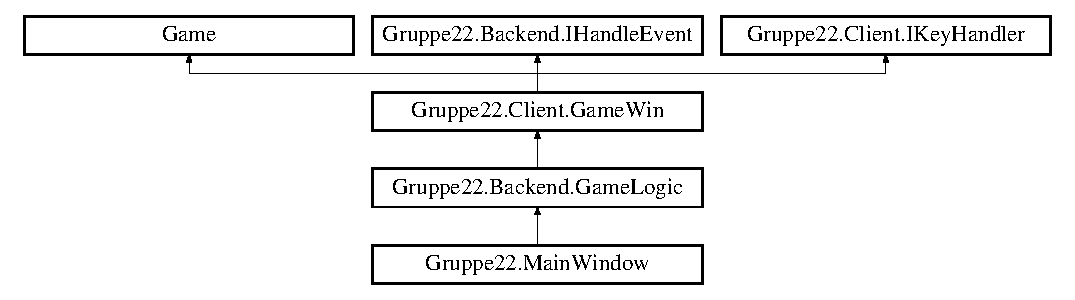
\includegraphics[height=3.589744cm]{class_gruppe22_1_1_backend_1_1_game_logic}
\end{center}
\end{figure}
\subsection*{Öffentliche Methoden}
\begin{DoxyCompactItemize}
\item 
override void \hyperlink{class_gruppe22_1_1_backend_1_1_game_logic_a44491c21e7048676d19f2e4dbfb2386c}{Handle\-Event} (bool Down\-Stream, \hyperlink{namespace_gruppe22_1_1_backend_ab56df91bb0bdafa1ea978e552209ce73}{Events} event\-I\-D, params object\mbox{[}$\,$\mbox{]} data)
\begin{DoxyCompactList}\small\item\em Handle events from U\-I\-Elements and/or backend objects \end{DoxyCompactList}\item 
void \hyperlink{class_gruppe22_1_1_backend_1_1_game_logic_a1be5667d5db7294fad1da32721f195ca}{Connect\-Rooms} (List$<$ \hyperlink{class_gruppe22_1_1_backend_1_1_generator}{Generator} $>$ rooms=null, int From=0, \hyperlink{namespace_gruppe22_1_1_backend_a2d53d5d14b8ea0951ba6971e5da1ebf5}{Direction} exit=Direction.\-None, int rooms\-Per\-Row=0)
\item 
void \hyperlink{class_gruppe22_1_1_backend_1_1_game_logic_a352d3b5b0d7c02cb73938e0464ee941a}{Connect\-Recursive} (List$<$ \hyperlink{class_gruppe22_1_1_backend_1_1_generator}{Generator} $>$ rooms, int id, List$<$ int $>$ visited=null)
\item 
void \hyperlink{class_gruppe22_1_1_backend_1_1_game_logic_aae4a27768f44fa3ee079eeda9f418990}{Show\-Message} (string message=\char`\"{}\char`\"{})
\begin{DoxyCompactList}\small\item\em A text displayed if the player died \end{DoxyCompactList}\item 
void \hyperlink{class_gruppe22_1_1_backend_1_1_game_logic_acaa73fcd270f74efde215829988df8ee}{Generate\-Maps} ()
\begin{DoxyCompactList}\small\item\em Generate three levels consisting of multiple rooms each and save them to xml files \end{DoxyCompactList}\end{DoxyCompactItemize}
\subsection*{Geschützte Methoden}
\begin{DoxyCompactItemize}
\item 
override void \hyperlink{class_gruppe22_1_1_backend_1_1_game_logic_afeba77d1e055f35a2abe58fcc849163d}{Initialize} ()
\begin{DoxyCompactList}\small\item\em Set up the (non visible) objects of the game \end{DoxyCompactList}\item 
void \hyperlink{class_gruppe22_1_1_backend_1_1_game_logic_a129959614d647372d87e8eb34e1c50a5}{\-\_\-\-Combat\-Damage} (int attacker, int defender)
\begin{DoxyCompactList}\small\item\em methode to evaluate the damage in a combat between two actors \end{DoxyCompactList}\item 
void \hyperlink{class_gruppe22_1_1_backend_1_1_game_logic_a7d29f64f2a93c336d262e017ef8d2f4b}{\-\_\-\-Trap\-Damage} (\hyperlink{class_gruppe22_1_1_backend_1_1_coords}{Coords} target)
\begin{DoxyCompactList}\small\item\em methode to evaluate the damage a trap deals to an actor walking over it or stands on raising trap \end{DoxyCompactList}\end{DoxyCompactItemize}
\subsection*{Weitere Geerbte Elemente}


\subsection{Ausführliche Beschreibung}
Handle game logic 



\subsection{Dokumentation der Elementfunktionen}
\hypertarget{class_gruppe22_1_1_backend_1_1_game_logic_a129959614d647372d87e8eb34e1c50a5}{\index{Gruppe22\-::\-Backend\-::\-Game\-Logic@{Gruppe22\-::\-Backend\-::\-Game\-Logic}!\-\_\-\-Combat\-Damage@{\-\_\-\-Combat\-Damage}}
\index{\-\_\-\-Combat\-Damage@{\-\_\-\-Combat\-Damage}!Gruppe22::Backend::GameLogic@{Gruppe22\-::\-Backend\-::\-Game\-Logic}}
\subsubsection[{\-\_\-\-Combat\-Damage}]{\setlength{\rightskip}{0pt plus 5cm}void Gruppe22.\-Backend.\-Game\-Logic.\-\_\-\-Combat\-Damage (
\begin{DoxyParamCaption}
\item[{int}]{attacker, }
\item[{int}]{defender}
\end{DoxyParamCaption}
)\hspace{0.3cm}{\ttfamily [protected]}}}\label{class_gruppe22_1_1_backend_1_1_game_logic_a129959614d647372d87e8eb34e1c50a5}


methode to evaluate the damage in a combat between two actors 


\begin{DoxyParams}{Parameter}
{\em attacker} & the attacking actor\\
\hline
{\em defender} & the attacked actor\\
\hline
\end{DoxyParams}
\hypertarget{class_gruppe22_1_1_backend_1_1_game_logic_a7d29f64f2a93c336d262e017ef8d2f4b}{\index{Gruppe22\-::\-Backend\-::\-Game\-Logic@{Gruppe22\-::\-Backend\-::\-Game\-Logic}!\-\_\-\-Trap\-Damage@{\-\_\-\-Trap\-Damage}}
\index{\-\_\-\-Trap\-Damage@{\-\_\-\-Trap\-Damage}!Gruppe22::Backend::GameLogic@{Gruppe22\-::\-Backend\-::\-Game\-Logic}}
\subsubsection[{\-\_\-\-Trap\-Damage}]{\setlength{\rightskip}{0pt plus 5cm}void Gruppe22.\-Backend.\-Game\-Logic.\-\_\-\-Trap\-Damage (
\begin{DoxyParamCaption}
\item[{{\bf Coords}}]{target}
\end{DoxyParamCaption}
)\hspace{0.3cm}{\ttfamily [protected]}}}\label{class_gruppe22_1_1_backend_1_1_game_logic_a7d29f64f2a93c336d262e017ef8d2f4b}


methode to evaluate the damage a trap deals to an actor walking over it or stands on raising trap 


\begin{DoxyParams}{Parameter}
{\em target} & \hyperlink{class_gruppe22_1_1_backend_1_1_coords}{Coords} of the actor which walked over the trap\\
\hline
\end{DoxyParams}
\hypertarget{class_gruppe22_1_1_backend_1_1_game_logic_a352d3b5b0d7c02cb73938e0464ee941a}{\index{Gruppe22\-::\-Backend\-::\-Game\-Logic@{Gruppe22\-::\-Backend\-::\-Game\-Logic}!Connect\-Recursive@{Connect\-Recursive}}
\index{Connect\-Recursive@{Connect\-Recursive}!Gruppe22::Backend::GameLogic@{Gruppe22\-::\-Backend\-::\-Game\-Logic}}
\subsubsection[{Connect\-Recursive}]{\setlength{\rightskip}{0pt plus 5cm}void Gruppe22.\-Backend.\-Game\-Logic.\-Connect\-Recursive (
\begin{DoxyParamCaption}
\item[{List$<$ {\bf Generator} $>$}]{rooms, }
\item[{int}]{id, }
\item[{List$<$ int $>$}]{visited = {\ttfamily null}}
\end{DoxyParamCaption}
)}}\label{class_gruppe22_1_1_backend_1_1_game_logic_a352d3b5b0d7c02cb73938e0464ee941a}
\hypertarget{class_gruppe22_1_1_backend_1_1_game_logic_a1be5667d5db7294fad1da32721f195ca}{\index{Gruppe22\-::\-Backend\-::\-Game\-Logic@{Gruppe22\-::\-Backend\-::\-Game\-Logic}!Connect\-Rooms@{Connect\-Rooms}}
\index{Connect\-Rooms@{Connect\-Rooms}!Gruppe22::Backend::GameLogic@{Gruppe22\-::\-Backend\-::\-Game\-Logic}}
\subsubsection[{Connect\-Rooms}]{\setlength{\rightskip}{0pt plus 5cm}void Gruppe22.\-Backend.\-Game\-Logic.\-Connect\-Rooms (
\begin{DoxyParamCaption}
\item[{List$<$ {\bf Generator} $>$}]{rooms = {\ttfamily null}, }
\item[{int}]{From = {\ttfamily 0}, }
\item[{{\bf Direction}}]{exit = {\ttfamily Direction.None}, }
\item[{int}]{rooms\-Per\-Row = {\ttfamily 0}}
\end{DoxyParamCaption}
)}}\label{class_gruppe22_1_1_backend_1_1_game_logic_a1be5667d5db7294fad1da32721f195ca}
\hypertarget{class_gruppe22_1_1_backend_1_1_game_logic_acaa73fcd270f74efde215829988df8ee}{\index{Gruppe22\-::\-Backend\-::\-Game\-Logic@{Gruppe22\-::\-Backend\-::\-Game\-Logic}!Generate\-Maps@{Generate\-Maps}}
\index{Generate\-Maps@{Generate\-Maps}!Gruppe22::Backend::GameLogic@{Gruppe22\-::\-Backend\-::\-Game\-Logic}}
\subsubsection[{Generate\-Maps}]{\setlength{\rightskip}{0pt plus 5cm}void Gruppe22.\-Backend.\-Game\-Logic.\-Generate\-Maps (
\begin{DoxyParamCaption}
{}
\end{DoxyParamCaption}
)}}\label{class_gruppe22_1_1_backend_1_1_game_logic_acaa73fcd270f74efde215829988df8ee}


Generate three levels consisting of multiple rooms each and save them to xml files 

\hypertarget{class_gruppe22_1_1_backend_1_1_game_logic_a44491c21e7048676d19f2e4dbfb2386c}{\index{Gruppe22\-::\-Backend\-::\-Game\-Logic@{Gruppe22\-::\-Backend\-::\-Game\-Logic}!Handle\-Event@{Handle\-Event}}
\index{Handle\-Event@{Handle\-Event}!Gruppe22::Backend::GameLogic@{Gruppe22\-::\-Backend\-::\-Game\-Logic}}
\subsubsection[{Handle\-Event}]{\setlength{\rightskip}{0pt plus 5cm}override void Gruppe22.\-Backend.\-Game\-Logic.\-Handle\-Event (
\begin{DoxyParamCaption}
\item[{bool}]{Down\-Stream, }
\item[{{\bf Events}}]{event\-I\-D, }
\item[{params object\mbox{[}$\,$\mbox{]}}]{data}
\end{DoxyParamCaption}
)}}\label{class_gruppe22_1_1_backend_1_1_game_logic_a44491c21e7048676d19f2e4dbfb2386c}


Handle events from U\-I\-Elements and/or backend objects 


\begin{DoxyParams}{Parameter}
{\em sender} & \\
\hline
{\em event\-I\-D} & \\
\hline
{\em data} & \\
\hline
\end{DoxyParams}
\hypertarget{class_gruppe22_1_1_backend_1_1_game_logic_afeba77d1e055f35a2abe58fcc849163d}{\index{Gruppe22\-::\-Backend\-::\-Game\-Logic@{Gruppe22\-::\-Backend\-::\-Game\-Logic}!Initialize@{Initialize}}
\index{Initialize@{Initialize}!Gruppe22::Backend::GameLogic@{Gruppe22\-::\-Backend\-::\-Game\-Logic}}
\subsubsection[{Initialize}]{\setlength{\rightskip}{0pt plus 5cm}override void Gruppe22.\-Backend.\-Game\-Logic.\-Initialize (
\begin{DoxyParamCaption}
{}
\end{DoxyParamCaption}
)\hspace{0.3cm}{\ttfamily [protected]}}}\label{class_gruppe22_1_1_backend_1_1_game_logic_afeba77d1e055f35a2abe58fcc849163d}


Set up the (non visible) objects of the game 

\hypertarget{class_gruppe22_1_1_backend_1_1_game_logic_aae4a27768f44fa3ee079eeda9f418990}{\index{Gruppe22\-::\-Backend\-::\-Game\-Logic@{Gruppe22\-::\-Backend\-::\-Game\-Logic}!Show\-Message@{Show\-Message}}
\index{Show\-Message@{Show\-Message}!Gruppe22::Backend::GameLogic@{Gruppe22\-::\-Backend\-::\-Game\-Logic}}
\subsubsection[{Show\-Message}]{\setlength{\rightskip}{0pt plus 5cm}void Gruppe22.\-Backend.\-Game\-Logic.\-Show\-Message (
\begin{DoxyParamCaption}
\item[{string}]{message = {\ttfamily \char`\"{}\char`\"{}}}
\end{DoxyParamCaption}
)}}\label{class_gruppe22_1_1_backend_1_1_game_logic_aae4a27768f44fa3ee079eeda9f418990}


A text displayed if the player died 


\begin{DoxyParams}{Parameter}
{\em message} & \\
\hline
{\em title} & \\
\hline
\end{DoxyParams}


Die Dokumentation für diese Klasse wurde erzeugt aufgrund der Datei\-:\begin{DoxyCompactItemize}
\item 
C\-:/\-Users/beursken/\-Documents/\-Git\-Hub/gruppe22/\-Gruppe22/\-Gruppe22/\-Backend/\hyperlink{_game_logic_8cs}{Game\-Logic.\-cs}\end{DoxyCompactItemize}

\hypertarget{class_gruppe22_1_1_client_1_1_game_win}{\section{Gruppe22.\-Client.\-Game\-Win Klassenreferenz}
\label{class_gruppe22_1_1_client_1_1_game_win}\index{Gruppe22.\-Client.\-Game\-Win@{Gruppe22.\-Client.\-Game\-Win}}
}


Handle all U\-I related operations of the game  


Klassendiagramm für Gruppe22.\-Client.\-Game\-Win\-:\begin{figure}[H]
\begin{center}
\leavevmode
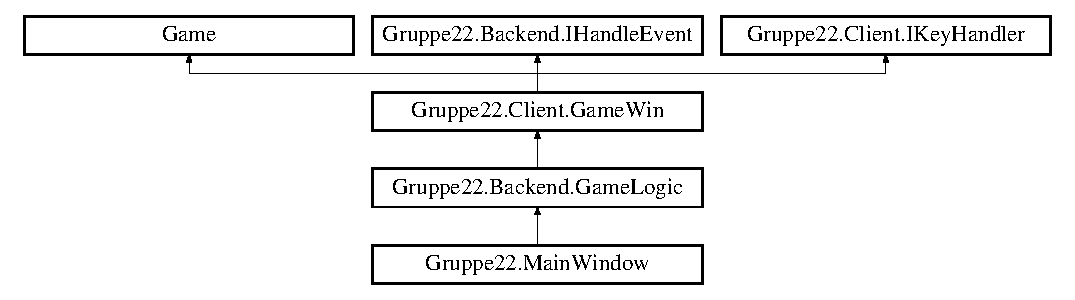
\includegraphics[height=3.589744cm]{class_gruppe22_1_1_client_1_1_game_win}
\end{center}
\end{figure}
\subsection*{Öffentliche Methoden}
\begin{DoxyCompactItemize}
\item 
bool \hyperlink{class_gruppe22_1_1_client_1_1_game_win_aba7e900502db9021072b1c85ec2f249a}{On\-Key\-Down} (Keys k)
\begin{DoxyCompactList}\small\item\em Called whenever a key was up and is now down \end{DoxyCompactList}\item 
bool \hyperlink{class_gruppe22_1_1_client_1_1_game_win_a9bab3243c9a2b2aaf135f0da6eac7ea3}{On\-Key\-Up} (Keys k)
\begin{DoxyCompactList}\small\item\em Called whenever a key was down and is now up \end{DoxyCompactList}\item 
bool \hyperlink{class_gruppe22_1_1_client_1_1_game_win_a62daf14bfc3ec358727ba46e12fa7167}{On\-Mouse\-Down} (int button)
\begin{DoxyCompactList}\small\item\em Called when a mouse button changes from up to down \end{DoxyCompactList}\item 
bool \hyperlink{class_gruppe22_1_1_client_1_1_game_win_a4adfd580aed6944cd2b286d3c6e768b9}{On\-Mouse\-Up} (int button)
\begin{DoxyCompactList}\small\item\em Called when a mouse button changes from down to up \end{DoxyCompactList}\item 
bool \hyperlink{class_gruppe22_1_1_client_1_1_game_win_ad9f9d99d868de3f6e7446524074856c9}{On\-Mouse\-Held} (int button)
\item 
bool \hyperlink{class_gruppe22_1_1_client_1_1_game_win_a9a74789da3ac1c1fa9ac35541db76c6d}{On\-Key\-Held} (Keys k)
\item 
virtual void \hyperlink{class_gruppe22_1_1_client_1_1_game_win_a47112e8228877ffb715cef2ec4e7ad21}{Handle\-Event} (bool Down\-Stream, \hyperlink{namespace_gruppe22_1_1_backend_ab56df91bb0bdafa1ea978e552209ce73}{Backend.\-Events} event\-I\-D, params object\mbox{[}$\,$\mbox{]} data)
\begin{DoxyCompactList}\small\item\em Handle events from U\-I\-Elements and/or backend objects \end{DoxyCompactList}\item 
void \hyperlink{class_gruppe22_1_1_client_1_1_game_win_acfebdc3931812064384ddcdb3f8567fc}{Show\-Menu} ()
\begin{DoxyCompactList}\small\item\em Display Main \hyperlink{class_gruppe22_1_1_client_1_1_menu}{Menu} \end{DoxyCompactList}\item 
void \hyperlink{class_gruppe22_1_1_client_1_1_game_win_a2ed19ead3fd36339afba5e0ff77bc2df}{Show\-Character\-Window} (\hyperlink{class_gruppe22_1_1_backend_1_1_actor}{Backend.\-Actor} actor, uint page=0)
\item 
void \hyperlink{class_gruppe22_1_1_client_1_1_game_win_af4563aa3977fbf62693b4ecdc83c22f1}{Show\-L\-A\-N\-Window} ()
\item 
void \hyperlink{class_gruppe22_1_1_client_1_1_game_win_a2774c7e13e85ef3d970f8bdf263d2e82}{Show\-Shop\-Window} (\hyperlink{class_gruppe22_1_1_backend_1_1_actor}{Backend.\-Actor} actor1, \hyperlink{class_gruppe22_1_1_backend_1_1_actor}{Backend.\-Actor} actor2)
\item 
void \hyperlink{class_gruppe22_1_1_client_1_1_game_win_abc9e6c78b7d6e60781ab1c1af3df56ec}{Show\-End\-Game} (string message=\char`\"{}You have failed in your mission. Better luck next time.\char`\"{}, string title=\char`\"{}Game over!\char`\"{})
\begin{DoxyCompactList}\small\item\em A text displayed if the player died \end{DoxyCompactList}\item 
void \hyperlink{class_gruppe22_1_1_client_1_1_game_win_a4104fdcc750ee89cb2a5422c6a61fd46}{Show\-About} ()
\begin{DoxyCompactList}\small\item\em Setup and display a window containing credits \end{DoxyCompactList}\item 
void \hyperlink{class_gruppe22_1_1_client_1_1_game_win_a902806ea43082fb2b47cded624f2c8e8}{wc\-\_\-\-Download\-Progress\-Changed} (object sender, Download\-Progress\-Changed\-Event\-Args e)
\begin{DoxyCompactList}\small\item\em Display download progress in the U\-I \end{DoxyCompactList}\item 
async void \hyperlink{class_gruppe22_1_1_client_1_1_game_win_acf9aac2989d7c1c1f53fb747829565aa}{wc\-\_\-\-Download\-File\-Completed} (object sender, System.\-Component\-Model.\-Async\-Completed\-Event\-Args e)
\begin{DoxyCompactList}\small\item\em Fired when a download is complete \end{DoxyCompactList}\item 
\hyperlink{class_gruppe22_1_1_client_1_1_game_win_a9d15393eb228404a0ad0ec3494acd623}{Game\-Win} ()
\begin{DoxyCompactList}\small\item\em Constructor \end{DoxyCompactList}\end{DoxyCompactItemize}
\subsection*{Geschützte Methoden}
\begin{DoxyCompactItemize}
\item 
override void \hyperlink{class_gruppe22_1_1_client_1_1_game_win_acbf872adf467819377ac4d1c408ca40d}{Initialize} ()
\begin{DoxyCompactList}\small\item\em Set up the (non visible) objects of the game \end{DoxyCompactList}\item 
void \hyperlink{class_gruppe22_1_1_client_1_1_game_win_aabf0b1516b698b9a512fb926722584e8}{Setup\-Game} ()
\item 
override void \hyperlink{class_gruppe22_1_1_client_1_1_game_win_a772c14a6b97580610d01d50f02731a02}{Load\-Content} ()
\begin{DoxyCompactList}\small\item\em Cache Content \end{DoxyCompactList}\item 
override void \hyperlink{class_gruppe22_1_1_client_1_1_game_win_ab95837e63a4d001504770a1ede94dc87}{Update} (Game\-Time game\-Time)
\begin{DoxyCompactList}\small\item\em Allows the game to run logic such as updating the world, checking for collisions, gathering input, and playing audio. \end{DoxyCompactList}\item 
override void \hyperlink{class_gruppe22_1_1_client_1_1_game_win_a97058890b16ef83f39bddf96d6a77717}{Draw} (Game\-Time game\-Time)
\begin{DoxyCompactList}\small\item\em This is called when the game should draw itself. \end{DoxyCompactList}\item 
override void \hyperlink{class_gruppe22_1_1_client_1_1_game_win_a3e49751dccbf4394ceaee838de7954d9}{Unload\-Content} ()
\begin{DoxyCompactList}\small\item\em Unload all managed content which has not been disposed of elsewhere \end{DoxyCompactList}\item 
void \hyperlink{class_gruppe22_1_1_client_1_1_game_win_a5d214c9143c57cc73655a286a673d848}{\-\_\-\-Add\-Message} (string s)
\begin{DoxyCompactList}\small\item\em Add text to status box \end{DoxyCompactList}\item 
void \hyperlink{class_gruppe22_1_1_client_1_1_game_win_a8bf0adab6f6d63c39d6d77133114391b}{\-\_\-\-Remove\-Health} ()
\begin{DoxyCompactList}\small\item\em Indicate damage done to player \end{DoxyCompactList}\item 
void \hyperlink{class_gruppe22_1_1_client_1_1_game_win_aa6cf8983ae2ac894e2755459c3f4aa85}{\-\_\-\-Add\-Health} ()
\begin{DoxyCompactList}\small\item\em Indicate health regained by potions \end{DoxyCompactList}\end{DoxyCompactItemize}
\subsection*{Geschützte Attribute}
\begin{DoxyCompactItemize}
\item 
Graphics\-Device\-Manager \hyperlink{class_gruppe22_1_1_client_1_1_game_win_aa40dabf43f3be876e3aec217cf20f4ee}{\-\_\-graphics} = null
\begin{DoxyCompactList}\small\item\em Central Output device \end{DoxyCompactList}\item 
Sprite\-Batch \hyperlink{class_gruppe22_1_1_client_1_1_game_win_af52be4e292a7ea1bf8b6f987ec31c52f}{\-\_\-sprite\-Batch} = null
\begin{DoxyCompactList}\small\item\em Central Sprite drawing algorithm \end{DoxyCompactList}\item 
int \hyperlink{class_gruppe22_1_1_client_1_1_game_win_a0aa22f5583a7f0e2ae97d8a33e8b9055}{\-\_\-deadcounter} = -\/1
\begin{DoxyCompactList}\small\item\em Count deads of player to load checkpoint or show gameover \end{DoxyCompactList}\item 
int \hyperlink{class_gruppe22_1_1_client_1_1_game_win_a07b8fca49486bb2e4946165899f027b3}{\-\_\-mouse\-Wheel} = 0
\begin{DoxyCompactList}\small\item\em Current mousewheel position (used to calculate changes) \end{DoxyCompactList}\item 
bool \hyperlink{class_gruppe22_1_1_client_1_1_game_win_a076f4987158764233c25585bcf62b730}{\-\_\-dragging} = false
\begin{DoxyCompactList}\small\item\em Whether the user is currently dragging something \end{DoxyCompactList}\item 
Vector2 \hyperlink{class_gruppe22_1_1_client_1_1_game_win_ae64e39fc0213b7db9121b53cf8bdb499}{\-\_\-mousepos} = Vector2.\-Zero
\begin{DoxyCompactList}\small\item\em Current position of mouse on screen \end{DoxyCompactList}\item 
List$<$ \hyperlink{class_gruppe22_1_1_client_1_1_u_i_element}{U\-I\-Element} $>$ \hyperlink{class_gruppe22_1_1_client_1_1_game_win_a65c32464243c130b3520ec347ff1659e}{\-\_\-interface\-Elements} = null
\begin{DoxyCompactList}\small\item\em A list of all elements displayed on screen \end{DoxyCompactList}\item 
\hyperlink{class_gruppe22_1_1_client_1_1_u_i_element}{U\-I\-Element} \hyperlink{class_gruppe22_1_1_client_1_1_game_win_a234b701077a7513f5a2f9d06bac40a17}{\-\_\-focus} = null
\begin{DoxyCompactList}\small\item\em The focussed element (to which input is passed) \end{DoxyCompactList}\item 
\hyperlink{class_gruppe22_1_1_backend_1_1_map}{Backend.\-Map} \hyperlink{class_gruppe22_1_1_client_1_1_game_win_a1389b978774586ee86471286cf271cc3}{\-\_\-map1} = null
\begin{DoxyCompactList}\small\item\em Internal storage for Player 1 \end{DoxyCompactList}\item 
\hyperlink{class_gruppe22_1_1_backend_1_1_map}{Backend.\-Map} \hyperlink{class_gruppe22_1_1_client_1_1_game_win_a4766437fe05165ffe55902c3eaa63025}{\-\_\-map2} = null
\begin{DoxyCompactList}\small\item\em Internal storage for Player 2 \end{DoxyCompactList}\item 
\hyperlink{namespace_gruppe22_1_1_backend_ad81bf4712f53c2ad4194343b6b0c73d2}{Backend.\-Game\-Status} \hyperlink{class_gruppe22_1_1_client_1_1_game_win_ac750d57d47285a3f2b1913b3ea784bdf}{\-\_\-status} = Backend.\-Game\-Status.\-Running
\begin{DoxyCompactList}\small\item\em Whether the game is paused (for menus etc.) \end{DoxyCompactList}\item 
Queue$<$ string $>$ \hyperlink{class_gruppe22_1_1_client_1_1_game_win_ab022cdc65543a866a781cdbc93882dd4}{\-\_\-files2fetch}
\begin{DoxyCompactList}\small\item\em A list of files to download \end{DoxyCompactList}\item 
Song \hyperlink{class_gruppe22_1_1_client_1_1_game_win_ac55e767d1594960d931ba76935659afe}{\-\_\-back\-Music}
\item 
\hyperlink{namespace_gruppe22_1_1_backend_ad81bf4712f53c2ad4194343b6b0c73d2}{Backend.\-Game\-Status} \hyperlink{class_gruppe22_1_1_client_1_1_game_win_a5ee0952fc213d5c3ae63698876a30ace}{\-\_\-prev\-State}
\begin{DoxyCompactList}\small\item\em Previous state (to reset after all files are downloaded) \end{DoxyCompactList}\item 
bool \hyperlink{class_gruppe22_1_1_client_1_1_game_win_af535ea47ceef795b292d3b831a628e32}{\-\_\-updating} = false
\begin{DoxyCompactList}\small\item\em True if update cycle is in progress (to prevent simultaneous changes) \end{DoxyCompactList}\item 
bool \hyperlink{class_gruppe22_1_1_client_1_1_game_win_a26adf6b2a5887176e083bace5b930d58}{\-\_\-drawing} = false
\begin{DoxyCompactList}\small\item\em True if currently drawing (to prevent superfluous redraws) \end{DoxyCompactList}\item 
Color \hyperlink{class_gruppe22_1_1_client_1_1_game_win_a1d439f242a800c7bf3dcf287bc2672d2}{\-\_\-backgroundcolor}
\begin{DoxyCompactList}\small\item\em Current background color (used to indicate healing or damage) \end{DoxyCompactList}\item 
Sprite\-Font \hyperlink{class_gruppe22_1_1_client_1_1_game_win_abb8bed1c5a9835889c4cf3cfdcf55565}{\-\_\-font}
\begin{DoxyCompactList}\small\item\em A spritefont used to display information on screen \end{DoxyCompactList}\item 
\hyperlink{class_gruppe22_1_1_client_1_1_mainmap}{Mainmap} \hyperlink{class_gruppe22_1_1_client_1_1_game_win_a8ca9d96b533860c16cfe62f37318c3f4}{\-\_\-mainmap1} = null
\begin{DoxyCompactList}\small\item\em The main map used for player 1 \end{DoxyCompactList}\item 
\hyperlink{class_gruppe22_1_1_client_1_1_minimap}{Minimap} \hyperlink{class_gruppe22_1_1_client_1_1_game_win_a9de92c080cdff45eee89ad8f647e8e82}{\-\_\-minimap1} = null
\begin{DoxyCompactList}\small\item\em A minimap \end{DoxyCompactList}\item 
\hyperlink{class_gruppe22_1_1_client_1_1_text_output}{Text\-Output} \hyperlink{class_gruppe22_1_1_client_1_1_game_win_a85609a2680f405bc25b355fd0c0c844f}{\-\_\-statusbox} = null
\begin{DoxyCompactList}\small\item\em The statusbox listing all messages / events \end{DoxyCompactList}\item 
\hyperlink{class_gruppe22_1_1_client_1_1_orb}{Orb} \hyperlink{class_gruppe22_1_1_client_1_1_game_win_a3d9da6069a5e5c60a810316a78c250a1}{\-\_\-health} = null
\item 
\hyperlink{class_gruppe22_1_1_client_1_1_orb}{Orb} \hyperlink{class_gruppe22_1_1_client_1_1_game_win_a131eb5cbd763f284409103fcf3240e25}{\-\_\-mana} = null
\item 
\hyperlink{class_gruppe22_1_1_client_1_1_toolbar}{Toolbar} \hyperlink{class_gruppe22_1_1_client_1_1_game_win_afd60e675c2675a7bf33ada1b98d93089}{\-\_\-toolbar} = null
\item 
\hyperlink{class_gruppe22_1_1_client_1_1_state_to_event}{State\-To\-Event} \hyperlink{class_gruppe22_1_1_client_1_1_game_win_ac886290b54c21246ed1617e50858f4a2}{\-\_\-events} = null
\begin{DoxyCompactList}\small\item\em Change-\/based handling of events (i.\-e. keyup/keydown) instead of status based (\char`\"{}\-Is key pressed?\char`\"{}) \end{DoxyCompactList}\item 
Random \hyperlink{class_gruppe22_1_1_client_1_1_game_win_af055bbaf549bd421da7f23068e009a10}{r} = null
\begin{DoxyCompactList}\small\item\em Random number generator \end{DoxyCompactList}\item 
List$<$ Sound\-Effect $>$ \hyperlink{class_gruppe22_1_1_client_1_1_game_win_a6763784b1678d11b7930be1dbcedc12e}{sound\-Effects} = null
\begin{DoxyCompactList}\small\item\em List of all sounds using in the Game \end{DoxyCompactList}\item 
string \hyperlink{class_gruppe22_1_1_client_1_1_game_win_a1d83df67b1c8ae9796477c3102b4c191}{\-\_\-downloading} = \char`\"{}\char`\"{}
\item 
\hyperlink{class_gruppe22_1_1_client_1_1_net_player}{Net\-Player} \hyperlink{class_gruppe22_1_1_client_1_1_game_win_a69d302e4a8d7839adbad2a3c9aa4baf9}{\-\_\-network} = null
\end{DoxyCompactItemize}


\subsection{Ausführliche Beschreibung}
Handle all U\-I related operations of the game 



\subsection{Beschreibung der Konstruktoren und Destruktoren}
\hypertarget{class_gruppe22_1_1_client_1_1_game_win_a9d15393eb228404a0ad0ec3494acd623}{\index{Gruppe22\-::\-Client\-::\-Game\-Win@{Gruppe22\-::\-Client\-::\-Game\-Win}!Game\-Win@{Game\-Win}}
\index{Game\-Win@{Game\-Win}!Gruppe22::Client::GameWin@{Gruppe22\-::\-Client\-::\-Game\-Win}}
\subsubsection[{Game\-Win}]{\setlength{\rightskip}{0pt plus 5cm}Gruppe22.\-Client.\-Game\-Win.\-Game\-Win (
\begin{DoxyParamCaption}
{}
\end{DoxyParamCaption}
)}}\label{class_gruppe22_1_1_client_1_1_game_win_a9d15393eb228404a0ad0ec3494acd623}


Constructor 



\subsection{Dokumentation der Elementfunktionen}
\hypertarget{class_gruppe22_1_1_client_1_1_game_win_aa6cf8983ae2ac894e2755459c3f4aa85}{\index{Gruppe22\-::\-Client\-::\-Game\-Win@{Gruppe22\-::\-Client\-::\-Game\-Win}!\-\_\-\-Add\-Health@{\-\_\-\-Add\-Health}}
\index{\-\_\-\-Add\-Health@{\-\_\-\-Add\-Health}!Gruppe22::Client::GameWin@{Gruppe22\-::\-Client\-::\-Game\-Win}}
\subsubsection[{\-\_\-\-Add\-Health}]{\setlength{\rightskip}{0pt plus 5cm}void Gruppe22.\-Client.\-Game\-Win.\-\_\-\-Add\-Health (
\begin{DoxyParamCaption}
{}
\end{DoxyParamCaption}
)\hspace{0.3cm}{\ttfamily [protected]}}}\label{class_gruppe22_1_1_client_1_1_game_win_aa6cf8983ae2ac894e2755459c3f4aa85}


Indicate health regained by potions 

\hypertarget{class_gruppe22_1_1_client_1_1_game_win_a5d214c9143c57cc73655a286a673d848}{\index{Gruppe22\-::\-Client\-::\-Game\-Win@{Gruppe22\-::\-Client\-::\-Game\-Win}!\-\_\-\-Add\-Message@{\-\_\-\-Add\-Message}}
\index{\-\_\-\-Add\-Message@{\-\_\-\-Add\-Message}!Gruppe22::Client::GameWin@{Gruppe22\-::\-Client\-::\-Game\-Win}}
\subsubsection[{\-\_\-\-Add\-Message}]{\setlength{\rightskip}{0pt plus 5cm}void Gruppe22.\-Client.\-Game\-Win.\-\_\-\-Add\-Message (
\begin{DoxyParamCaption}
\item[{string}]{s}
\end{DoxyParamCaption}
)\hspace{0.3cm}{\ttfamily [protected]}}}\label{class_gruppe22_1_1_client_1_1_game_win_a5d214c9143c57cc73655a286a673d848}


Add text to status box 


\begin{DoxyParams}{Parameter}
{\em s} & \\
\hline
\end{DoxyParams}
\hypertarget{class_gruppe22_1_1_client_1_1_game_win_a8bf0adab6f6d63c39d6d77133114391b}{\index{Gruppe22\-::\-Client\-::\-Game\-Win@{Gruppe22\-::\-Client\-::\-Game\-Win}!\-\_\-\-Remove\-Health@{\-\_\-\-Remove\-Health}}
\index{\-\_\-\-Remove\-Health@{\-\_\-\-Remove\-Health}!Gruppe22::Client::GameWin@{Gruppe22\-::\-Client\-::\-Game\-Win}}
\subsubsection[{\-\_\-\-Remove\-Health}]{\setlength{\rightskip}{0pt plus 5cm}void Gruppe22.\-Client.\-Game\-Win.\-\_\-\-Remove\-Health (
\begin{DoxyParamCaption}
{}
\end{DoxyParamCaption}
)\hspace{0.3cm}{\ttfamily [protected]}}}\label{class_gruppe22_1_1_client_1_1_game_win_a8bf0adab6f6d63c39d6d77133114391b}


Indicate damage done to player 

\hypertarget{class_gruppe22_1_1_client_1_1_game_win_a97058890b16ef83f39bddf96d6a77717}{\index{Gruppe22\-::\-Client\-::\-Game\-Win@{Gruppe22\-::\-Client\-::\-Game\-Win}!Draw@{Draw}}
\index{Draw@{Draw}!Gruppe22::Client::GameWin@{Gruppe22\-::\-Client\-::\-Game\-Win}}
\subsubsection[{Draw}]{\setlength{\rightskip}{0pt plus 5cm}override void Gruppe22.\-Client.\-Game\-Win.\-Draw (
\begin{DoxyParamCaption}
\item[{Game\-Time}]{game\-Time}
\end{DoxyParamCaption}
)\hspace{0.3cm}{\ttfamily [protected]}}}\label{class_gruppe22_1_1_client_1_1_game_win_a97058890b16ef83f39bddf96d6a77717}


This is called when the game should draw itself. 


\begin{DoxyParams}{Parameter}
{\em game\-Time} & Provides a snapshot of timing values.\\
\hline
\end{DoxyParams}
\hypertarget{class_gruppe22_1_1_client_1_1_game_win_a47112e8228877ffb715cef2ec4e7ad21}{\index{Gruppe22\-::\-Client\-::\-Game\-Win@{Gruppe22\-::\-Client\-::\-Game\-Win}!Handle\-Event@{Handle\-Event}}
\index{Handle\-Event@{Handle\-Event}!Gruppe22::Client::GameWin@{Gruppe22\-::\-Client\-::\-Game\-Win}}
\subsubsection[{Handle\-Event}]{\setlength{\rightskip}{0pt plus 5cm}virtual void Gruppe22.\-Client.\-Game\-Win.\-Handle\-Event (
\begin{DoxyParamCaption}
\item[{bool}]{Down\-Stream, }
\item[{{\bf Backend.\-Events}}]{event\-I\-D, }
\item[{params object\mbox{[}$\,$\mbox{]}}]{data}
\end{DoxyParamCaption}
)\hspace{0.3cm}{\ttfamily [virtual]}}}\label{class_gruppe22_1_1_client_1_1_game_win_a47112e8228877ffb715cef2ec4e7ad21}


Handle events from U\-I\-Elements and/or backend objects 


\begin{DoxyParams}{Parameter}
{\em sender} & \\
\hline
{\em event\-I\-D} & \\
\hline
{\em data} & \\
\hline
\end{DoxyParams}
\hypertarget{class_gruppe22_1_1_client_1_1_game_win_acbf872adf467819377ac4d1c408ca40d}{\index{Gruppe22\-::\-Client\-::\-Game\-Win@{Gruppe22\-::\-Client\-::\-Game\-Win}!Initialize@{Initialize}}
\index{Initialize@{Initialize}!Gruppe22::Client::GameWin@{Gruppe22\-::\-Client\-::\-Game\-Win}}
\subsubsection[{Initialize}]{\setlength{\rightskip}{0pt plus 5cm}override void Gruppe22.\-Client.\-Game\-Win.\-Initialize (
\begin{DoxyParamCaption}
{}
\end{DoxyParamCaption}
)\hspace{0.3cm}{\ttfamily [protected]}}}\label{class_gruppe22_1_1_client_1_1_game_win_acbf872adf467819377ac4d1c408ca40d}


Set up the (non visible) objects of the game 

\hypertarget{class_gruppe22_1_1_client_1_1_game_win_a772c14a6b97580610d01d50f02731a02}{\index{Gruppe22\-::\-Client\-::\-Game\-Win@{Gruppe22\-::\-Client\-::\-Game\-Win}!Load\-Content@{Load\-Content}}
\index{Load\-Content@{Load\-Content}!Gruppe22::Client::GameWin@{Gruppe22\-::\-Client\-::\-Game\-Win}}
\subsubsection[{Load\-Content}]{\setlength{\rightskip}{0pt plus 5cm}override void Gruppe22.\-Client.\-Game\-Win.\-Load\-Content (
\begin{DoxyParamCaption}
{}
\end{DoxyParamCaption}
)\hspace{0.3cm}{\ttfamily [protected]}}}\label{class_gruppe22_1_1_client_1_1_game_win_a772c14a6b97580610d01d50f02731a02}


Cache Content 

\hypertarget{class_gruppe22_1_1_client_1_1_game_win_aba7e900502db9021072b1c85ec2f249a}{\index{Gruppe22\-::\-Client\-::\-Game\-Win@{Gruppe22\-::\-Client\-::\-Game\-Win}!On\-Key\-Down@{On\-Key\-Down}}
\index{On\-Key\-Down@{On\-Key\-Down}!Gruppe22::Client::GameWin@{Gruppe22\-::\-Client\-::\-Game\-Win}}
\subsubsection[{On\-Key\-Down}]{\setlength{\rightskip}{0pt plus 5cm}bool Gruppe22.\-Client.\-Game\-Win.\-On\-Key\-Down (
\begin{DoxyParamCaption}
\item[{Keys}]{k}
\end{DoxyParamCaption}
)}}\label{class_gruppe22_1_1_client_1_1_game_win_aba7e900502db9021072b1c85ec2f249a}


Called whenever a key was up and is now down 


\begin{DoxyParams}{Parameter}
{\em k} & The key which was pressed\\
\hline
\end{DoxyParams}


Implementiert \hyperlink{interface_gruppe22_1_1_client_1_1_i_key_handler_a3816611e429cab857650f672fda4632b}{Gruppe22.\-Client.\-I\-Key\-Handler}.

\hypertarget{class_gruppe22_1_1_client_1_1_game_win_a9a74789da3ac1c1fa9ac35541db76c6d}{\index{Gruppe22\-::\-Client\-::\-Game\-Win@{Gruppe22\-::\-Client\-::\-Game\-Win}!On\-Key\-Held@{On\-Key\-Held}}
\index{On\-Key\-Held@{On\-Key\-Held}!Gruppe22::Client::GameWin@{Gruppe22\-::\-Client\-::\-Game\-Win}}
\subsubsection[{On\-Key\-Held}]{\setlength{\rightskip}{0pt plus 5cm}bool Gruppe22.\-Client.\-Game\-Win.\-On\-Key\-Held (
\begin{DoxyParamCaption}
\item[{Keys}]{k}
\end{DoxyParamCaption}
)}}\label{class_gruppe22_1_1_client_1_1_game_win_a9a74789da3ac1c1fa9ac35541db76c6d}


Implementiert \hyperlink{interface_gruppe22_1_1_client_1_1_i_key_handler_a4196bd333be759f8ade7996f58ca39d6}{Gruppe22.\-Client.\-I\-Key\-Handler}.

\hypertarget{class_gruppe22_1_1_client_1_1_game_win_a9bab3243c9a2b2aaf135f0da6eac7ea3}{\index{Gruppe22\-::\-Client\-::\-Game\-Win@{Gruppe22\-::\-Client\-::\-Game\-Win}!On\-Key\-Up@{On\-Key\-Up}}
\index{On\-Key\-Up@{On\-Key\-Up}!Gruppe22::Client::GameWin@{Gruppe22\-::\-Client\-::\-Game\-Win}}
\subsubsection[{On\-Key\-Up}]{\setlength{\rightskip}{0pt plus 5cm}bool Gruppe22.\-Client.\-Game\-Win.\-On\-Key\-Up (
\begin{DoxyParamCaption}
\item[{Keys}]{k}
\end{DoxyParamCaption}
)}}\label{class_gruppe22_1_1_client_1_1_game_win_a9bab3243c9a2b2aaf135f0da6eac7ea3}


Called whenever a key was down and is now up 


\begin{DoxyParams}{Parameter}
{\em k} & The key which was pressed\\
\hline
\end{DoxyParams}


Implementiert \hyperlink{interface_gruppe22_1_1_client_1_1_i_key_handler_adf473af0ebd0c8a3a22ba252ed381356}{Gruppe22.\-Client.\-I\-Key\-Handler}.

\hypertarget{class_gruppe22_1_1_client_1_1_game_win_a62daf14bfc3ec358727ba46e12fa7167}{\index{Gruppe22\-::\-Client\-::\-Game\-Win@{Gruppe22\-::\-Client\-::\-Game\-Win}!On\-Mouse\-Down@{On\-Mouse\-Down}}
\index{On\-Mouse\-Down@{On\-Mouse\-Down}!Gruppe22::Client::GameWin@{Gruppe22\-::\-Client\-::\-Game\-Win}}
\subsubsection[{On\-Mouse\-Down}]{\setlength{\rightskip}{0pt plus 5cm}bool Gruppe22.\-Client.\-Game\-Win.\-On\-Mouse\-Down (
\begin{DoxyParamCaption}
\item[{int}]{button}
\end{DoxyParamCaption}
)}}\label{class_gruppe22_1_1_client_1_1_game_win_a62daf14bfc3ec358727ba46e12fa7167}


Called when a mouse button changes from up to down 


\begin{DoxyParams}{Parameter}
{\em button} & Left \hyperlink{class_gruppe22_1_1_client_1_1_button}{Button}=1, Middle \hyperlink{class_gruppe22_1_1_client_1_1_button}{Button}=2, Right \hyperlink{class_gruppe22_1_1_client_1_1_button}{Button}=3\\
\hline
\end{DoxyParams}


Implementiert \hyperlink{interface_gruppe22_1_1_client_1_1_i_key_handler_a6e52139cdd4408abdd31e61ce1e69991}{Gruppe22.\-Client.\-I\-Key\-Handler}.

\hypertarget{class_gruppe22_1_1_client_1_1_game_win_ad9f9d99d868de3f6e7446524074856c9}{\index{Gruppe22\-::\-Client\-::\-Game\-Win@{Gruppe22\-::\-Client\-::\-Game\-Win}!On\-Mouse\-Held@{On\-Mouse\-Held}}
\index{On\-Mouse\-Held@{On\-Mouse\-Held}!Gruppe22::Client::GameWin@{Gruppe22\-::\-Client\-::\-Game\-Win}}
\subsubsection[{On\-Mouse\-Held}]{\setlength{\rightskip}{0pt plus 5cm}bool Gruppe22.\-Client.\-Game\-Win.\-On\-Mouse\-Held (
\begin{DoxyParamCaption}
\item[{int}]{button}
\end{DoxyParamCaption}
)}}\label{class_gruppe22_1_1_client_1_1_game_win_ad9f9d99d868de3f6e7446524074856c9}


Implementiert \hyperlink{interface_gruppe22_1_1_client_1_1_i_key_handler_aa66a6080c4ea14b63a5578882b9f3b3e}{Gruppe22.\-Client.\-I\-Key\-Handler}.

\hypertarget{class_gruppe22_1_1_client_1_1_game_win_a4adfd580aed6944cd2b286d3c6e768b9}{\index{Gruppe22\-::\-Client\-::\-Game\-Win@{Gruppe22\-::\-Client\-::\-Game\-Win}!On\-Mouse\-Up@{On\-Mouse\-Up}}
\index{On\-Mouse\-Up@{On\-Mouse\-Up}!Gruppe22::Client::GameWin@{Gruppe22\-::\-Client\-::\-Game\-Win}}
\subsubsection[{On\-Mouse\-Up}]{\setlength{\rightskip}{0pt plus 5cm}bool Gruppe22.\-Client.\-Game\-Win.\-On\-Mouse\-Up (
\begin{DoxyParamCaption}
\item[{int}]{button}
\end{DoxyParamCaption}
)}}\label{class_gruppe22_1_1_client_1_1_game_win_a4adfd580aed6944cd2b286d3c6e768b9}


Called when a mouse button changes from down to up 


\begin{DoxyParams}{Parameter}
{\em button} & Left \hyperlink{class_gruppe22_1_1_client_1_1_button}{Button}=1, Middle \hyperlink{class_gruppe22_1_1_client_1_1_button}{Button}=2, Right \hyperlink{class_gruppe22_1_1_client_1_1_button}{Button}=3\\
\hline
\end{DoxyParams}


Implementiert \hyperlink{interface_gruppe22_1_1_client_1_1_i_key_handler_ad1fd9aa17fc6f8328beddd59cef28499}{Gruppe22.\-Client.\-I\-Key\-Handler}.

\hypertarget{class_gruppe22_1_1_client_1_1_game_win_aabf0b1516b698b9a512fb926722584e8}{\index{Gruppe22\-::\-Client\-::\-Game\-Win@{Gruppe22\-::\-Client\-::\-Game\-Win}!Setup\-Game@{Setup\-Game}}
\index{Setup\-Game@{Setup\-Game}!Gruppe22::Client::GameWin@{Gruppe22\-::\-Client\-::\-Game\-Win}}
\subsubsection[{Setup\-Game}]{\setlength{\rightskip}{0pt plus 5cm}void Gruppe22.\-Client.\-Game\-Win.\-Setup\-Game (
\begin{DoxyParamCaption}
{}
\end{DoxyParamCaption}
)\hspace{0.3cm}{\ttfamily [protected]}}}\label{class_gruppe22_1_1_client_1_1_game_win_aabf0b1516b698b9a512fb926722584e8}
\hypertarget{class_gruppe22_1_1_client_1_1_game_win_a4104fdcc750ee89cb2a5422c6a61fd46}{\index{Gruppe22\-::\-Client\-::\-Game\-Win@{Gruppe22\-::\-Client\-::\-Game\-Win}!Show\-About@{Show\-About}}
\index{Show\-About@{Show\-About}!Gruppe22::Client::GameWin@{Gruppe22\-::\-Client\-::\-Game\-Win}}
\subsubsection[{Show\-About}]{\setlength{\rightskip}{0pt plus 5cm}void Gruppe22.\-Client.\-Game\-Win.\-Show\-About (
\begin{DoxyParamCaption}
{}
\end{DoxyParamCaption}
)}}\label{class_gruppe22_1_1_client_1_1_game_win_a4104fdcc750ee89cb2a5422c6a61fd46}


Setup and display a window containing credits 

\hypertarget{class_gruppe22_1_1_client_1_1_game_win_a2ed19ead3fd36339afba5e0ff77bc2df}{\index{Gruppe22\-::\-Client\-::\-Game\-Win@{Gruppe22\-::\-Client\-::\-Game\-Win}!Show\-Character\-Window@{Show\-Character\-Window}}
\index{Show\-Character\-Window@{Show\-Character\-Window}!Gruppe22::Client::GameWin@{Gruppe22\-::\-Client\-::\-Game\-Win}}
\subsubsection[{Show\-Character\-Window}]{\setlength{\rightskip}{0pt plus 5cm}void Gruppe22.\-Client.\-Game\-Win.\-Show\-Character\-Window (
\begin{DoxyParamCaption}
\item[{{\bf Backend.\-Actor}}]{actor, }
\item[{uint}]{page = {\ttfamily 0}}
\end{DoxyParamCaption}
)}}\label{class_gruppe22_1_1_client_1_1_game_win_a2ed19ead3fd36339afba5e0ff77bc2df}
\hypertarget{class_gruppe22_1_1_client_1_1_game_win_abc9e6c78b7d6e60781ab1c1af3df56ec}{\index{Gruppe22\-::\-Client\-::\-Game\-Win@{Gruppe22\-::\-Client\-::\-Game\-Win}!Show\-End\-Game@{Show\-End\-Game}}
\index{Show\-End\-Game@{Show\-End\-Game}!Gruppe22::Client::GameWin@{Gruppe22\-::\-Client\-::\-Game\-Win}}
\subsubsection[{Show\-End\-Game}]{\setlength{\rightskip}{0pt plus 5cm}void Gruppe22.\-Client.\-Game\-Win.\-Show\-End\-Game (
\begin{DoxyParamCaption}
\item[{string}]{message = {\ttfamily \char`\"{}You~have~failed~in~your~mission.~Better~luck~next~time.\char`\"{}}, }
\item[{string}]{title = {\ttfamily \char`\"{}Game~over!\char`\"{}}}
\end{DoxyParamCaption}
)}}\label{class_gruppe22_1_1_client_1_1_game_win_abc9e6c78b7d6e60781ab1c1af3df56ec}


A text displayed if the player died 


\begin{DoxyParams}{Parameter}
{\em message} & \\
\hline
{\em title} & \\
\hline
\end{DoxyParams}
\hypertarget{class_gruppe22_1_1_client_1_1_game_win_af4563aa3977fbf62693b4ecdc83c22f1}{\index{Gruppe22\-::\-Client\-::\-Game\-Win@{Gruppe22\-::\-Client\-::\-Game\-Win}!Show\-L\-A\-N\-Window@{Show\-L\-A\-N\-Window}}
\index{Show\-L\-A\-N\-Window@{Show\-L\-A\-N\-Window}!Gruppe22::Client::GameWin@{Gruppe22\-::\-Client\-::\-Game\-Win}}
\subsubsection[{Show\-L\-A\-N\-Window}]{\setlength{\rightskip}{0pt plus 5cm}void Gruppe22.\-Client.\-Game\-Win.\-Show\-L\-A\-N\-Window (
\begin{DoxyParamCaption}
{}
\end{DoxyParamCaption}
)}}\label{class_gruppe22_1_1_client_1_1_game_win_af4563aa3977fbf62693b4ecdc83c22f1}
\hypertarget{class_gruppe22_1_1_client_1_1_game_win_acfebdc3931812064384ddcdb3f8567fc}{\index{Gruppe22\-::\-Client\-::\-Game\-Win@{Gruppe22\-::\-Client\-::\-Game\-Win}!Show\-Menu@{Show\-Menu}}
\index{Show\-Menu@{Show\-Menu}!Gruppe22::Client::GameWin@{Gruppe22\-::\-Client\-::\-Game\-Win}}
\subsubsection[{Show\-Menu}]{\setlength{\rightskip}{0pt plus 5cm}void Gruppe22.\-Client.\-Game\-Win.\-Show\-Menu (
\begin{DoxyParamCaption}
{}
\end{DoxyParamCaption}
)}}\label{class_gruppe22_1_1_client_1_1_game_win_acfebdc3931812064384ddcdb3f8567fc}


Display Main \hyperlink{class_gruppe22_1_1_client_1_1_menu}{Menu} 

\hypertarget{class_gruppe22_1_1_client_1_1_game_win_a2774c7e13e85ef3d970f8bdf263d2e82}{\index{Gruppe22\-::\-Client\-::\-Game\-Win@{Gruppe22\-::\-Client\-::\-Game\-Win}!Show\-Shop\-Window@{Show\-Shop\-Window}}
\index{Show\-Shop\-Window@{Show\-Shop\-Window}!Gruppe22::Client::GameWin@{Gruppe22\-::\-Client\-::\-Game\-Win}}
\subsubsection[{Show\-Shop\-Window}]{\setlength{\rightskip}{0pt plus 5cm}void Gruppe22.\-Client.\-Game\-Win.\-Show\-Shop\-Window (
\begin{DoxyParamCaption}
\item[{{\bf Backend.\-Actor}}]{actor1, }
\item[{{\bf Backend.\-Actor}}]{actor2}
\end{DoxyParamCaption}
)}}\label{class_gruppe22_1_1_client_1_1_game_win_a2774c7e13e85ef3d970f8bdf263d2e82}
\hypertarget{class_gruppe22_1_1_client_1_1_game_win_a3e49751dccbf4394ceaee838de7954d9}{\index{Gruppe22\-::\-Client\-::\-Game\-Win@{Gruppe22\-::\-Client\-::\-Game\-Win}!Unload\-Content@{Unload\-Content}}
\index{Unload\-Content@{Unload\-Content}!Gruppe22::Client::GameWin@{Gruppe22\-::\-Client\-::\-Game\-Win}}
\subsubsection[{Unload\-Content}]{\setlength{\rightskip}{0pt plus 5cm}override void Gruppe22.\-Client.\-Game\-Win.\-Unload\-Content (
\begin{DoxyParamCaption}
{}
\end{DoxyParamCaption}
)\hspace{0.3cm}{\ttfamily [protected]}}}\label{class_gruppe22_1_1_client_1_1_game_win_a3e49751dccbf4394ceaee838de7954d9}


Unload all managed content which has not been disposed of elsewhere 

\hypertarget{class_gruppe22_1_1_client_1_1_game_win_ab95837e63a4d001504770a1ede94dc87}{\index{Gruppe22\-::\-Client\-::\-Game\-Win@{Gruppe22\-::\-Client\-::\-Game\-Win}!Update@{Update}}
\index{Update@{Update}!Gruppe22::Client::GameWin@{Gruppe22\-::\-Client\-::\-Game\-Win}}
\subsubsection[{Update}]{\setlength{\rightskip}{0pt plus 5cm}override void Gruppe22.\-Client.\-Game\-Win.\-Update (
\begin{DoxyParamCaption}
\item[{Game\-Time}]{game\-Time}
\end{DoxyParamCaption}
)\hspace{0.3cm}{\ttfamily [protected]}}}\label{class_gruppe22_1_1_client_1_1_game_win_ab95837e63a4d001504770a1ede94dc87}


Allows the game to run logic such as updating the world, checking for collisions, gathering input, and playing audio. 


\begin{DoxyParams}{Parameter}
{\em game\-Time} & Provides a snapshot of timing values.\\
\hline
\end{DoxyParams}
\hypertarget{class_gruppe22_1_1_client_1_1_game_win_acf9aac2989d7c1c1f53fb747829565aa}{\index{Gruppe22\-::\-Client\-::\-Game\-Win@{Gruppe22\-::\-Client\-::\-Game\-Win}!wc\-\_\-\-Download\-File\-Completed@{wc\-\_\-\-Download\-File\-Completed}}
\index{wc\-\_\-\-Download\-File\-Completed@{wc\-\_\-\-Download\-File\-Completed}!Gruppe22::Client::GameWin@{Gruppe22\-::\-Client\-::\-Game\-Win}}
\subsubsection[{wc\-\_\-\-Download\-File\-Completed}]{\setlength{\rightskip}{0pt plus 5cm}async void Gruppe22.\-Client.\-Game\-Win.\-wc\-\_\-\-Download\-File\-Completed (
\begin{DoxyParamCaption}
\item[{object}]{sender, }
\item[{System.\-Component\-Model.\-Async\-Completed\-Event\-Args}]{e}
\end{DoxyParamCaption}
)}}\label{class_gruppe22_1_1_client_1_1_game_win_acf9aac2989d7c1c1f53fb747829565aa}


Fired when a download is complete 


\begin{DoxyParams}{Parameter}
{\em sender} & The source of the event\\
\hline
{\em e} & Event data\\
\hline
\end{DoxyParams}
\hypertarget{class_gruppe22_1_1_client_1_1_game_win_a902806ea43082fb2b47cded624f2c8e8}{\index{Gruppe22\-::\-Client\-::\-Game\-Win@{Gruppe22\-::\-Client\-::\-Game\-Win}!wc\-\_\-\-Download\-Progress\-Changed@{wc\-\_\-\-Download\-Progress\-Changed}}
\index{wc\-\_\-\-Download\-Progress\-Changed@{wc\-\_\-\-Download\-Progress\-Changed}!Gruppe22::Client::GameWin@{Gruppe22\-::\-Client\-::\-Game\-Win}}
\subsubsection[{wc\-\_\-\-Download\-Progress\-Changed}]{\setlength{\rightskip}{0pt plus 5cm}void Gruppe22.\-Client.\-Game\-Win.\-wc\-\_\-\-Download\-Progress\-Changed (
\begin{DoxyParamCaption}
\item[{object}]{sender, }
\item[{Download\-Progress\-Changed\-Event\-Args}]{e}
\end{DoxyParamCaption}
)}}\label{class_gruppe22_1_1_client_1_1_game_win_a902806ea43082fb2b47cded624f2c8e8}


Display download progress in the U\-I 


\begin{DoxyParams}{Parameter}
{\em sender} & The source of the event\\
\hline
{\em e} & Event data\\
\hline
\end{DoxyParams}


\subsection{Dokumentation der Datenelemente}
\hypertarget{class_gruppe22_1_1_client_1_1_game_win_a1d439f242a800c7bf3dcf287bc2672d2}{\index{Gruppe22\-::\-Client\-::\-Game\-Win@{Gruppe22\-::\-Client\-::\-Game\-Win}!\-\_\-backgroundcolor@{\-\_\-backgroundcolor}}
\index{\-\_\-backgroundcolor@{\-\_\-backgroundcolor}!Gruppe22::Client::GameWin@{Gruppe22\-::\-Client\-::\-Game\-Win}}
\subsubsection[{\-\_\-backgroundcolor}]{\setlength{\rightskip}{0pt plus 5cm}Color Gruppe22.\-Client.\-Game\-Win.\-\_\-backgroundcolor\hspace{0.3cm}{\ttfamily [protected]}}}\label{class_gruppe22_1_1_client_1_1_game_win_a1d439f242a800c7bf3dcf287bc2672d2}


Current background color (used to indicate healing or damage) 

\hypertarget{class_gruppe22_1_1_client_1_1_game_win_ac55e767d1594960d931ba76935659afe}{\index{Gruppe22\-::\-Client\-::\-Game\-Win@{Gruppe22\-::\-Client\-::\-Game\-Win}!\-\_\-back\-Music@{\-\_\-back\-Music}}
\index{\-\_\-back\-Music@{\-\_\-back\-Music}!Gruppe22::Client::GameWin@{Gruppe22\-::\-Client\-::\-Game\-Win}}
\subsubsection[{\-\_\-back\-Music}]{\setlength{\rightskip}{0pt plus 5cm}Song Gruppe22.\-Client.\-Game\-Win.\-\_\-back\-Music\hspace{0.3cm}{\ttfamily [protected]}}}\label{class_gruppe22_1_1_client_1_1_game_win_ac55e767d1594960d931ba76935659afe}
\hypertarget{class_gruppe22_1_1_client_1_1_game_win_a0aa22f5583a7f0e2ae97d8a33e8b9055}{\index{Gruppe22\-::\-Client\-::\-Game\-Win@{Gruppe22\-::\-Client\-::\-Game\-Win}!\-\_\-deadcounter@{\-\_\-deadcounter}}
\index{\-\_\-deadcounter@{\-\_\-deadcounter}!Gruppe22::Client::GameWin@{Gruppe22\-::\-Client\-::\-Game\-Win}}
\subsubsection[{\-\_\-deadcounter}]{\setlength{\rightskip}{0pt plus 5cm}int Gruppe22.\-Client.\-Game\-Win.\-\_\-deadcounter = -\/1\hspace{0.3cm}{\ttfamily [protected]}}}\label{class_gruppe22_1_1_client_1_1_game_win_a0aa22f5583a7f0e2ae97d8a33e8b9055}


Count deads of player to load checkpoint or show gameover 

\hypertarget{class_gruppe22_1_1_client_1_1_game_win_a1d83df67b1c8ae9796477c3102b4c191}{\index{Gruppe22\-::\-Client\-::\-Game\-Win@{Gruppe22\-::\-Client\-::\-Game\-Win}!\-\_\-downloading@{\-\_\-downloading}}
\index{\-\_\-downloading@{\-\_\-downloading}!Gruppe22::Client::GameWin@{Gruppe22\-::\-Client\-::\-Game\-Win}}
\subsubsection[{\-\_\-downloading}]{\setlength{\rightskip}{0pt plus 5cm}string Gruppe22.\-Client.\-Game\-Win.\-\_\-downloading = \char`\"{}\char`\"{}\hspace{0.3cm}{\ttfamily [protected]}}}\label{class_gruppe22_1_1_client_1_1_game_win_a1d83df67b1c8ae9796477c3102b4c191}
\hypertarget{class_gruppe22_1_1_client_1_1_game_win_a076f4987158764233c25585bcf62b730}{\index{Gruppe22\-::\-Client\-::\-Game\-Win@{Gruppe22\-::\-Client\-::\-Game\-Win}!\-\_\-dragging@{\-\_\-dragging}}
\index{\-\_\-dragging@{\-\_\-dragging}!Gruppe22::Client::GameWin@{Gruppe22\-::\-Client\-::\-Game\-Win}}
\subsubsection[{\-\_\-dragging}]{\setlength{\rightskip}{0pt plus 5cm}bool Gruppe22.\-Client.\-Game\-Win.\-\_\-dragging = false\hspace{0.3cm}{\ttfamily [protected]}}}\label{class_gruppe22_1_1_client_1_1_game_win_a076f4987158764233c25585bcf62b730}


Whether the user is currently dragging something 

\hypertarget{class_gruppe22_1_1_client_1_1_game_win_a26adf6b2a5887176e083bace5b930d58}{\index{Gruppe22\-::\-Client\-::\-Game\-Win@{Gruppe22\-::\-Client\-::\-Game\-Win}!\-\_\-drawing@{\-\_\-drawing}}
\index{\-\_\-drawing@{\-\_\-drawing}!Gruppe22::Client::GameWin@{Gruppe22\-::\-Client\-::\-Game\-Win}}
\subsubsection[{\-\_\-drawing}]{\setlength{\rightskip}{0pt plus 5cm}bool Gruppe22.\-Client.\-Game\-Win.\-\_\-drawing = false\hspace{0.3cm}{\ttfamily [protected]}}}\label{class_gruppe22_1_1_client_1_1_game_win_a26adf6b2a5887176e083bace5b930d58}


True if currently drawing (to prevent superfluous redraws) 

\hypertarget{class_gruppe22_1_1_client_1_1_game_win_ac886290b54c21246ed1617e50858f4a2}{\index{Gruppe22\-::\-Client\-::\-Game\-Win@{Gruppe22\-::\-Client\-::\-Game\-Win}!\-\_\-events@{\-\_\-events}}
\index{\-\_\-events@{\-\_\-events}!Gruppe22::Client::GameWin@{Gruppe22\-::\-Client\-::\-Game\-Win}}
\subsubsection[{\-\_\-events}]{\setlength{\rightskip}{0pt plus 5cm}{\bf State\-To\-Event} Gruppe22.\-Client.\-Game\-Win.\-\_\-events = null\hspace{0.3cm}{\ttfamily [protected]}}}\label{class_gruppe22_1_1_client_1_1_game_win_ac886290b54c21246ed1617e50858f4a2}


Change-\/based handling of events (i.\-e. keyup/keydown) instead of status based (\char`\"{}\-Is key pressed?\char`\"{}) 

\hypertarget{class_gruppe22_1_1_client_1_1_game_win_ab022cdc65543a866a781cdbc93882dd4}{\index{Gruppe22\-::\-Client\-::\-Game\-Win@{Gruppe22\-::\-Client\-::\-Game\-Win}!\-\_\-files2fetch@{\-\_\-files2fetch}}
\index{\-\_\-files2fetch@{\-\_\-files2fetch}!Gruppe22::Client::GameWin@{Gruppe22\-::\-Client\-::\-Game\-Win}}
\subsubsection[{\-\_\-files2fetch}]{\setlength{\rightskip}{0pt plus 5cm}Queue$<$string$>$ Gruppe22.\-Client.\-Game\-Win.\-\_\-files2fetch\hspace{0.3cm}{\ttfamily [protected]}}}\label{class_gruppe22_1_1_client_1_1_game_win_ab022cdc65543a866a781cdbc93882dd4}


A list of files to download 

\hypertarget{class_gruppe22_1_1_client_1_1_game_win_a234b701077a7513f5a2f9d06bac40a17}{\index{Gruppe22\-::\-Client\-::\-Game\-Win@{Gruppe22\-::\-Client\-::\-Game\-Win}!\-\_\-focus@{\-\_\-focus}}
\index{\-\_\-focus@{\-\_\-focus}!Gruppe22::Client::GameWin@{Gruppe22\-::\-Client\-::\-Game\-Win}}
\subsubsection[{\-\_\-focus}]{\setlength{\rightskip}{0pt plus 5cm}{\bf U\-I\-Element} Gruppe22.\-Client.\-Game\-Win.\-\_\-focus = null\hspace{0.3cm}{\ttfamily [protected]}}}\label{class_gruppe22_1_1_client_1_1_game_win_a234b701077a7513f5a2f9d06bac40a17}


The focussed element (to which input is passed) 

\hypertarget{class_gruppe22_1_1_client_1_1_game_win_abb8bed1c5a9835889c4cf3cfdcf55565}{\index{Gruppe22\-::\-Client\-::\-Game\-Win@{Gruppe22\-::\-Client\-::\-Game\-Win}!\-\_\-font@{\-\_\-font}}
\index{\-\_\-font@{\-\_\-font}!Gruppe22::Client::GameWin@{Gruppe22\-::\-Client\-::\-Game\-Win}}
\subsubsection[{\-\_\-font}]{\setlength{\rightskip}{0pt plus 5cm}Sprite\-Font Gruppe22.\-Client.\-Game\-Win.\-\_\-font\hspace{0.3cm}{\ttfamily [protected]}}}\label{class_gruppe22_1_1_client_1_1_game_win_abb8bed1c5a9835889c4cf3cfdcf55565}


A spritefont used to display information on screen 

\hypertarget{class_gruppe22_1_1_client_1_1_game_win_aa40dabf43f3be876e3aec217cf20f4ee}{\index{Gruppe22\-::\-Client\-::\-Game\-Win@{Gruppe22\-::\-Client\-::\-Game\-Win}!\-\_\-graphics@{\-\_\-graphics}}
\index{\-\_\-graphics@{\-\_\-graphics}!Gruppe22::Client::GameWin@{Gruppe22\-::\-Client\-::\-Game\-Win}}
\subsubsection[{\-\_\-graphics}]{\setlength{\rightskip}{0pt plus 5cm}Graphics\-Device\-Manager Gruppe22.\-Client.\-Game\-Win.\-\_\-graphics = null\hspace{0.3cm}{\ttfamily [protected]}}}\label{class_gruppe22_1_1_client_1_1_game_win_aa40dabf43f3be876e3aec217cf20f4ee}


Central Output device 

\hypertarget{class_gruppe22_1_1_client_1_1_game_win_a3d9da6069a5e5c60a810316a78c250a1}{\index{Gruppe22\-::\-Client\-::\-Game\-Win@{Gruppe22\-::\-Client\-::\-Game\-Win}!\-\_\-health@{\-\_\-health}}
\index{\-\_\-health@{\-\_\-health}!Gruppe22::Client::GameWin@{Gruppe22\-::\-Client\-::\-Game\-Win}}
\subsubsection[{\-\_\-health}]{\setlength{\rightskip}{0pt plus 5cm}{\bf Orb} Gruppe22.\-Client.\-Game\-Win.\-\_\-health = null\hspace{0.3cm}{\ttfamily [protected]}}}\label{class_gruppe22_1_1_client_1_1_game_win_a3d9da6069a5e5c60a810316a78c250a1}
\hypertarget{class_gruppe22_1_1_client_1_1_game_win_a65c32464243c130b3520ec347ff1659e}{\index{Gruppe22\-::\-Client\-::\-Game\-Win@{Gruppe22\-::\-Client\-::\-Game\-Win}!\-\_\-interface\-Elements@{\-\_\-interface\-Elements}}
\index{\-\_\-interface\-Elements@{\-\_\-interface\-Elements}!Gruppe22::Client::GameWin@{Gruppe22\-::\-Client\-::\-Game\-Win}}
\subsubsection[{\-\_\-interface\-Elements}]{\setlength{\rightskip}{0pt plus 5cm}List$<${\bf U\-I\-Element}$>$ Gruppe22.\-Client.\-Game\-Win.\-\_\-interface\-Elements = null\hspace{0.3cm}{\ttfamily [protected]}}}\label{class_gruppe22_1_1_client_1_1_game_win_a65c32464243c130b3520ec347ff1659e}


A list of all elements displayed on screen 

\hypertarget{class_gruppe22_1_1_client_1_1_game_win_a8ca9d96b533860c16cfe62f37318c3f4}{\index{Gruppe22\-::\-Client\-::\-Game\-Win@{Gruppe22\-::\-Client\-::\-Game\-Win}!\-\_\-mainmap1@{\-\_\-mainmap1}}
\index{\-\_\-mainmap1@{\-\_\-mainmap1}!Gruppe22::Client::GameWin@{Gruppe22\-::\-Client\-::\-Game\-Win}}
\subsubsection[{\-\_\-mainmap1}]{\setlength{\rightskip}{0pt plus 5cm}{\bf Mainmap} Gruppe22.\-Client.\-Game\-Win.\-\_\-mainmap1 = null\hspace{0.3cm}{\ttfamily [protected]}}}\label{class_gruppe22_1_1_client_1_1_game_win_a8ca9d96b533860c16cfe62f37318c3f4}


The main map used for player 1 

\hypertarget{class_gruppe22_1_1_client_1_1_game_win_a131eb5cbd763f284409103fcf3240e25}{\index{Gruppe22\-::\-Client\-::\-Game\-Win@{Gruppe22\-::\-Client\-::\-Game\-Win}!\-\_\-mana@{\-\_\-mana}}
\index{\-\_\-mana@{\-\_\-mana}!Gruppe22::Client::GameWin@{Gruppe22\-::\-Client\-::\-Game\-Win}}
\subsubsection[{\-\_\-mana}]{\setlength{\rightskip}{0pt plus 5cm}{\bf Orb} Gruppe22.\-Client.\-Game\-Win.\-\_\-mana = null\hspace{0.3cm}{\ttfamily [protected]}}}\label{class_gruppe22_1_1_client_1_1_game_win_a131eb5cbd763f284409103fcf3240e25}
\hypertarget{class_gruppe22_1_1_client_1_1_game_win_a1389b978774586ee86471286cf271cc3}{\index{Gruppe22\-::\-Client\-::\-Game\-Win@{Gruppe22\-::\-Client\-::\-Game\-Win}!\-\_\-map1@{\-\_\-map1}}
\index{\-\_\-map1@{\-\_\-map1}!Gruppe22::Client::GameWin@{Gruppe22\-::\-Client\-::\-Game\-Win}}
\subsubsection[{\-\_\-map1}]{\setlength{\rightskip}{0pt plus 5cm}{\bf Backend.\-Map} Gruppe22.\-Client.\-Game\-Win.\-\_\-map1 = null\hspace{0.3cm}{\ttfamily [protected]}}}\label{class_gruppe22_1_1_client_1_1_game_win_a1389b978774586ee86471286cf271cc3}


Internal storage for Player 1 

\hypertarget{class_gruppe22_1_1_client_1_1_game_win_a4766437fe05165ffe55902c3eaa63025}{\index{Gruppe22\-::\-Client\-::\-Game\-Win@{Gruppe22\-::\-Client\-::\-Game\-Win}!\-\_\-map2@{\-\_\-map2}}
\index{\-\_\-map2@{\-\_\-map2}!Gruppe22::Client::GameWin@{Gruppe22\-::\-Client\-::\-Game\-Win}}
\subsubsection[{\-\_\-map2}]{\setlength{\rightskip}{0pt plus 5cm}{\bf Backend.\-Map} Gruppe22.\-Client.\-Game\-Win.\-\_\-map2 = null\hspace{0.3cm}{\ttfamily [protected]}}}\label{class_gruppe22_1_1_client_1_1_game_win_a4766437fe05165ffe55902c3eaa63025}


Internal storage for Player 2 

\hypertarget{class_gruppe22_1_1_client_1_1_game_win_a9de92c080cdff45eee89ad8f647e8e82}{\index{Gruppe22\-::\-Client\-::\-Game\-Win@{Gruppe22\-::\-Client\-::\-Game\-Win}!\-\_\-minimap1@{\-\_\-minimap1}}
\index{\-\_\-minimap1@{\-\_\-minimap1}!Gruppe22::Client::GameWin@{Gruppe22\-::\-Client\-::\-Game\-Win}}
\subsubsection[{\-\_\-minimap1}]{\setlength{\rightskip}{0pt plus 5cm}{\bf Minimap} Gruppe22.\-Client.\-Game\-Win.\-\_\-minimap1 = null\hspace{0.3cm}{\ttfamily [protected]}}}\label{class_gruppe22_1_1_client_1_1_game_win_a9de92c080cdff45eee89ad8f647e8e82}


A minimap 

\hypertarget{class_gruppe22_1_1_client_1_1_game_win_ae64e39fc0213b7db9121b53cf8bdb499}{\index{Gruppe22\-::\-Client\-::\-Game\-Win@{Gruppe22\-::\-Client\-::\-Game\-Win}!\-\_\-mousepos@{\-\_\-mousepos}}
\index{\-\_\-mousepos@{\-\_\-mousepos}!Gruppe22::Client::GameWin@{Gruppe22\-::\-Client\-::\-Game\-Win}}
\subsubsection[{\-\_\-mousepos}]{\setlength{\rightskip}{0pt plus 5cm}Vector2 Gruppe22.\-Client.\-Game\-Win.\-\_\-mousepos = Vector2.\-Zero\hspace{0.3cm}{\ttfamily [protected]}}}\label{class_gruppe22_1_1_client_1_1_game_win_ae64e39fc0213b7db9121b53cf8bdb499}


Current position of mouse on screen 

\hypertarget{class_gruppe22_1_1_client_1_1_game_win_a07b8fca49486bb2e4946165899f027b3}{\index{Gruppe22\-::\-Client\-::\-Game\-Win@{Gruppe22\-::\-Client\-::\-Game\-Win}!\-\_\-mouse\-Wheel@{\-\_\-mouse\-Wheel}}
\index{\-\_\-mouse\-Wheel@{\-\_\-mouse\-Wheel}!Gruppe22::Client::GameWin@{Gruppe22\-::\-Client\-::\-Game\-Win}}
\subsubsection[{\-\_\-mouse\-Wheel}]{\setlength{\rightskip}{0pt plus 5cm}int Gruppe22.\-Client.\-Game\-Win.\-\_\-mouse\-Wheel = 0\hspace{0.3cm}{\ttfamily [protected]}}}\label{class_gruppe22_1_1_client_1_1_game_win_a07b8fca49486bb2e4946165899f027b3}


Current mousewheel position (used to calculate changes) 

\hypertarget{class_gruppe22_1_1_client_1_1_game_win_a69d302e4a8d7839adbad2a3c9aa4baf9}{\index{Gruppe22\-::\-Client\-::\-Game\-Win@{Gruppe22\-::\-Client\-::\-Game\-Win}!\-\_\-network@{\-\_\-network}}
\index{\-\_\-network@{\-\_\-network}!Gruppe22::Client::GameWin@{Gruppe22\-::\-Client\-::\-Game\-Win}}
\subsubsection[{\-\_\-network}]{\setlength{\rightskip}{0pt plus 5cm}{\bf Net\-Player} Gruppe22.\-Client.\-Game\-Win.\-\_\-network = null\hspace{0.3cm}{\ttfamily [protected]}}}\label{class_gruppe22_1_1_client_1_1_game_win_a69d302e4a8d7839adbad2a3c9aa4baf9}
\hypertarget{class_gruppe22_1_1_client_1_1_game_win_a5ee0952fc213d5c3ae63698876a30ace}{\index{Gruppe22\-::\-Client\-::\-Game\-Win@{Gruppe22\-::\-Client\-::\-Game\-Win}!\-\_\-prev\-State@{\-\_\-prev\-State}}
\index{\-\_\-prev\-State@{\-\_\-prev\-State}!Gruppe22::Client::GameWin@{Gruppe22\-::\-Client\-::\-Game\-Win}}
\subsubsection[{\-\_\-prev\-State}]{\setlength{\rightskip}{0pt plus 5cm}{\bf Backend.\-Game\-Status} Gruppe22.\-Client.\-Game\-Win.\-\_\-prev\-State\hspace{0.3cm}{\ttfamily [protected]}}}\label{class_gruppe22_1_1_client_1_1_game_win_a5ee0952fc213d5c3ae63698876a30ace}


Previous state (to reset after all files are downloaded) 

\hypertarget{class_gruppe22_1_1_client_1_1_game_win_af52be4e292a7ea1bf8b6f987ec31c52f}{\index{Gruppe22\-::\-Client\-::\-Game\-Win@{Gruppe22\-::\-Client\-::\-Game\-Win}!\-\_\-sprite\-Batch@{\-\_\-sprite\-Batch}}
\index{\-\_\-sprite\-Batch@{\-\_\-sprite\-Batch}!Gruppe22::Client::GameWin@{Gruppe22\-::\-Client\-::\-Game\-Win}}
\subsubsection[{\-\_\-sprite\-Batch}]{\setlength{\rightskip}{0pt plus 5cm}Sprite\-Batch Gruppe22.\-Client.\-Game\-Win.\-\_\-sprite\-Batch = null\hspace{0.3cm}{\ttfamily [protected]}}}\label{class_gruppe22_1_1_client_1_1_game_win_af52be4e292a7ea1bf8b6f987ec31c52f}


Central Sprite drawing algorithm 

\hypertarget{class_gruppe22_1_1_client_1_1_game_win_ac750d57d47285a3f2b1913b3ea784bdf}{\index{Gruppe22\-::\-Client\-::\-Game\-Win@{Gruppe22\-::\-Client\-::\-Game\-Win}!\-\_\-status@{\-\_\-status}}
\index{\-\_\-status@{\-\_\-status}!Gruppe22::Client::GameWin@{Gruppe22\-::\-Client\-::\-Game\-Win}}
\subsubsection[{\-\_\-status}]{\setlength{\rightskip}{0pt plus 5cm}{\bf Backend.\-Game\-Status} Gruppe22.\-Client.\-Game\-Win.\-\_\-status = Backend.\-Game\-Status.\-Running\hspace{0.3cm}{\ttfamily [protected]}}}\label{class_gruppe22_1_1_client_1_1_game_win_ac750d57d47285a3f2b1913b3ea784bdf}


Whether the game is paused (for menus etc.) 

\hypertarget{class_gruppe22_1_1_client_1_1_game_win_a85609a2680f405bc25b355fd0c0c844f}{\index{Gruppe22\-::\-Client\-::\-Game\-Win@{Gruppe22\-::\-Client\-::\-Game\-Win}!\-\_\-statusbox@{\-\_\-statusbox}}
\index{\-\_\-statusbox@{\-\_\-statusbox}!Gruppe22::Client::GameWin@{Gruppe22\-::\-Client\-::\-Game\-Win}}
\subsubsection[{\-\_\-statusbox}]{\setlength{\rightskip}{0pt plus 5cm}{\bf Text\-Output} Gruppe22.\-Client.\-Game\-Win.\-\_\-statusbox = null\hspace{0.3cm}{\ttfamily [protected]}}}\label{class_gruppe22_1_1_client_1_1_game_win_a85609a2680f405bc25b355fd0c0c844f}


The statusbox listing all messages / events 

\hypertarget{class_gruppe22_1_1_client_1_1_game_win_afd60e675c2675a7bf33ada1b98d93089}{\index{Gruppe22\-::\-Client\-::\-Game\-Win@{Gruppe22\-::\-Client\-::\-Game\-Win}!\-\_\-toolbar@{\-\_\-toolbar}}
\index{\-\_\-toolbar@{\-\_\-toolbar}!Gruppe22::Client::GameWin@{Gruppe22\-::\-Client\-::\-Game\-Win}}
\subsubsection[{\-\_\-toolbar}]{\setlength{\rightskip}{0pt plus 5cm}{\bf Toolbar} Gruppe22.\-Client.\-Game\-Win.\-\_\-toolbar = null\hspace{0.3cm}{\ttfamily [protected]}}}\label{class_gruppe22_1_1_client_1_1_game_win_afd60e675c2675a7bf33ada1b98d93089}
\hypertarget{class_gruppe22_1_1_client_1_1_game_win_af535ea47ceef795b292d3b831a628e32}{\index{Gruppe22\-::\-Client\-::\-Game\-Win@{Gruppe22\-::\-Client\-::\-Game\-Win}!\-\_\-updating@{\-\_\-updating}}
\index{\-\_\-updating@{\-\_\-updating}!Gruppe22::Client::GameWin@{Gruppe22\-::\-Client\-::\-Game\-Win}}
\subsubsection[{\-\_\-updating}]{\setlength{\rightskip}{0pt plus 5cm}bool Gruppe22.\-Client.\-Game\-Win.\-\_\-updating = false\hspace{0.3cm}{\ttfamily [protected]}}}\label{class_gruppe22_1_1_client_1_1_game_win_af535ea47ceef795b292d3b831a628e32}


True if update cycle is in progress (to prevent simultaneous changes) 

\hypertarget{class_gruppe22_1_1_client_1_1_game_win_af055bbaf549bd421da7f23068e009a10}{\index{Gruppe22\-::\-Client\-::\-Game\-Win@{Gruppe22\-::\-Client\-::\-Game\-Win}!r@{r}}
\index{r@{r}!Gruppe22::Client::GameWin@{Gruppe22\-::\-Client\-::\-Game\-Win}}
\subsubsection[{r}]{\setlength{\rightskip}{0pt plus 5cm}Random Gruppe22.\-Client.\-Game\-Win.\-r = null\hspace{0.3cm}{\ttfamily [protected]}}}\label{class_gruppe22_1_1_client_1_1_game_win_af055bbaf549bd421da7f23068e009a10}


Random number generator 

\hypertarget{class_gruppe22_1_1_client_1_1_game_win_a6763784b1678d11b7930be1dbcedc12e}{\index{Gruppe22\-::\-Client\-::\-Game\-Win@{Gruppe22\-::\-Client\-::\-Game\-Win}!sound\-Effects@{sound\-Effects}}
\index{sound\-Effects@{sound\-Effects}!Gruppe22::Client::GameWin@{Gruppe22\-::\-Client\-::\-Game\-Win}}
\subsubsection[{sound\-Effects}]{\setlength{\rightskip}{0pt plus 5cm}List$<$Sound\-Effect$>$ Gruppe22.\-Client.\-Game\-Win.\-sound\-Effects = null\hspace{0.3cm}{\ttfamily [protected]}}}\label{class_gruppe22_1_1_client_1_1_game_win_a6763784b1678d11b7930be1dbcedc12e}


List of all sounds using in the Game 



Die Dokumentation für diese Klasse wurde erzeugt aufgrund der Datei\-:\begin{DoxyCompactItemize}
\item 
C\-:/\-Users/beursken/\-Documents/\-Git\-Hub/gruppe22/\-Gruppe22/\-Gruppe22/\-Client/\-U\-I/\hyperlink{_game_win_8cs}{Game\-Win.\-cs}\end{DoxyCompactItemize}

\hypertarget{class_gruppe22_1_1_backend_1_1_gap_tile}{\section{Gruppe22.\-Backend.\-Gap\-Tile Klassenreferenz}
\label{class_gruppe22_1_1_backend_1_1_gap_tile}\index{Gruppe22.\-Backend.\-Gap\-Tile@{Gruppe22.\-Backend.\-Gap\-Tile}}
}
Klassendiagramm für Gruppe22.\-Backend.\-Gap\-Tile\-:\begin{figure}[H]
\begin{center}
\leavevmode
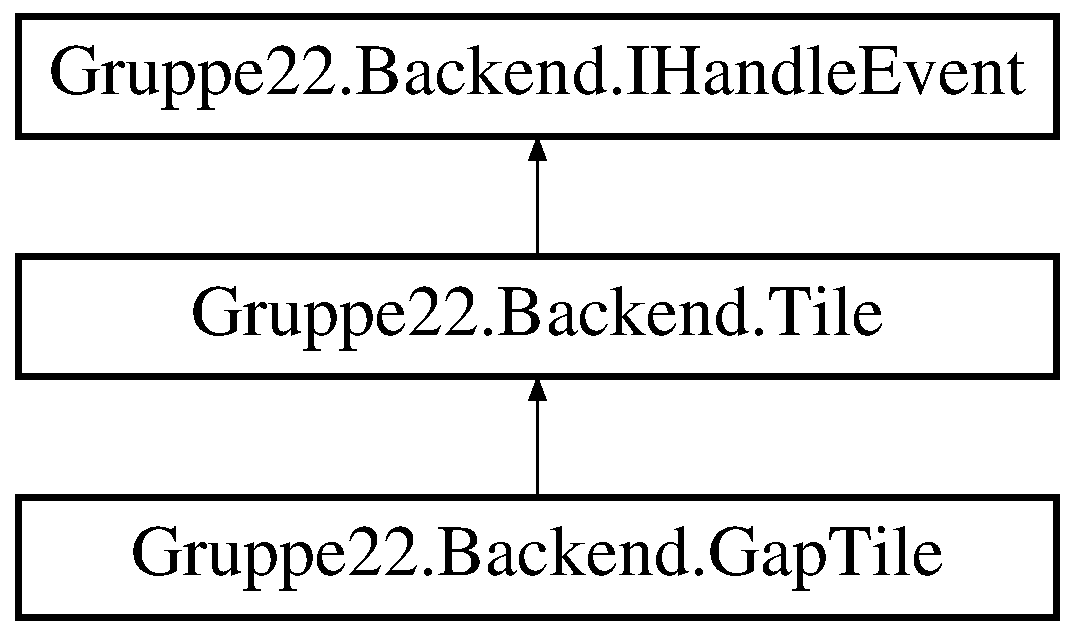
\includegraphics[height=3.000000cm]{class_gruppe22_1_1_backend_1_1_gap_tile}
\end{center}
\end{figure}
\subsection*{Öffentliche Methoden}
\begin{DoxyCompactItemize}
\item 
override void \hyperlink{class_gruppe22_1_1_backend_1_1_gap_tile_aeeed4e7d3d3d230ba20398bee17f4ed2}{Save} (Xml\-Writer xmlw)
\begin{DoxyCompactList}\small\item\em Abstract method to save a tile in a X\-M\-L file \end{DoxyCompactList}\item 
\hyperlink{class_gruppe22_1_1_backend_1_1_gap_tile_a6ae54dae7bf37a807d01e7c449b43e2c}{Gap\-Tile} (object \hyperlink{class_gruppe22_1_1_backend_1_1_tile_abc12933c70eb3a2ebbb2fde9f45c2632}{parent})
\end{DoxyCompactItemize}
\subsection*{Propertys}
\begin{DoxyCompactItemize}
\item 
int \hyperlink{class_gruppe22_1_1_backend_1_1_gap_tile_a2833c0484bcea6f07f1643bb44137116}{style}\hspace{0.3cm}{\ttfamily  \mbox{[}get, set\mbox{]}}
\end{DoxyCompactItemize}
\subsection*{Weitere Geerbte Elemente}


\subsection{Beschreibung der Konstruktoren und Destruktoren}
\hypertarget{class_gruppe22_1_1_backend_1_1_gap_tile_a6ae54dae7bf37a807d01e7c449b43e2c}{\index{Gruppe22\-::\-Backend\-::\-Gap\-Tile@{Gruppe22\-::\-Backend\-::\-Gap\-Tile}!Gap\-Tile@{Gap\-Tile}}
\index{Gap\-Tile@{Gap\-Tile}!Gruppe22::Backend::GapTile@{Gruppe22\-::\-Backend\-::\-Gap\-Tile}}
\subsubsection[{Gap\-Tile}]{\setlength{\rightskip}{0pt plus 5cm}Gruppe22.\-Backend.\-Gap\-Tile.\-Gap\-Tile (
\begin{DoxyParamCaption}
\item[{object}]{parent}
\end{DoxyParamCaption}
)}}\label{class_gruppe22_1_1_backend_1_1_gap_tile_a6ae54dae7bf37a807d01e7c449b43e2c}


\subsection{Dokumentation der Elementfunktionen}
\hypertarget{class_gruppe22_1_1_backend_1_1_gap_tile_aeeed4e7d3d3d230ba20398bee17f4ed2}{\index{Gruppe22\-::\-Backend\-::\-Gap\-Tile@{Gruppe22\-::\-Backend\-::\-Gap\-Tile}!Save@{Save}}
\index{Save@{Save}!Gruppe22::Backend::GapTile@{Gruppe22\-::\-Backend\-::\-Gap\-Tile}}
\subsubsection[{Save}]{\setlength{\rightskip}{0pt plus 5cm}override void Gruppe22.\-Backend.\-Gap\-Tile.\-Save (
\begin{DoxyParamCaption}
\item[{Xml\-Writer}]{xmlw}
\end{DoxyParamCaption}
)\hspace{0.3cm}{\ttfamily [virtual]}}}\label{class_gruppe22_1_1_backend_1_1_gap_tile_aeeed4e7d3d3d230ba20398bee17f4ed2}


Abstract method to save a tile in a X\-M\-L file 


\begin{DoxyParams}{Parameter}
{\em xmlw} & the Xml\-Writer used for saving the file\\
\hline
\end{DoxyParams}


Erneute Implementation von \hyperlink{class_gruppe22_1_1_backend_1_1_tile_a109ab3e77ffca9d44c95a711af3491dc}{Gruppe22.\-Backend.\-Tile}.



\subsection{Dokumentation der Propertys}
\hypertarget{class_gruppe22_1_1_backend_1_1_gap_tile_a2833c0484bcea6f07f1643bb44137116}{\index{Gruppe22\-::\-Backend\-::\-Gap\-Tile@{Gruppe22\-::\-Backend\-::\-Gap\-Tile}!style@{style}}
\index{style@{style}!Gruppe22::Backend::GapTile@{Gruppe22\-::\-Backend\-::\-Gap\-Tile}}
\subsubsection[{style}]{\setlength{\rightskip}{0pt plus 5cm}int Gruppe22.\-Backend.\-Gap\-Tile.\-style\hspace{0.3cm}{\ttfamily [get]}, {\ttfamily [set]}}}\label{class_gruppe22_1_1_backend_1_1_gap_tile_a2833c0484bcea6f07f1643bb44137116}


Die Dokumentation für diese Klasse wurde erzeugt aufgrund der Datei\-:\begin{DoxyCompactItemize}
\item 
C\-:/\-Users/beursken/\-Documents/\-Git\-Hub/gruppe22/\-Gruppe22/\-Gruppe22/\-Backend/\-Map/\hyperlink{_gap_tile_8cs}{Gap\-Tile.\-cs}\end{DoxyCompactItemize}

\hypertarget{class_gruppe22_1_1_backend_1_1_generator}{\section{Gruppe22.\-Backend.\-Generator Klassenreferenz}
\label{class_gruppe22_1_1_backend_1_1_generator}\index{Gruppe22.\-Backend.\-Generator@{Gruppe22.\-Backend.\-Generator}}
}
Klassendiagramm für Gruppe22.\-Backend.\-Generator\-:\begin{figure}[H]
\begin{center}
\leavevmode
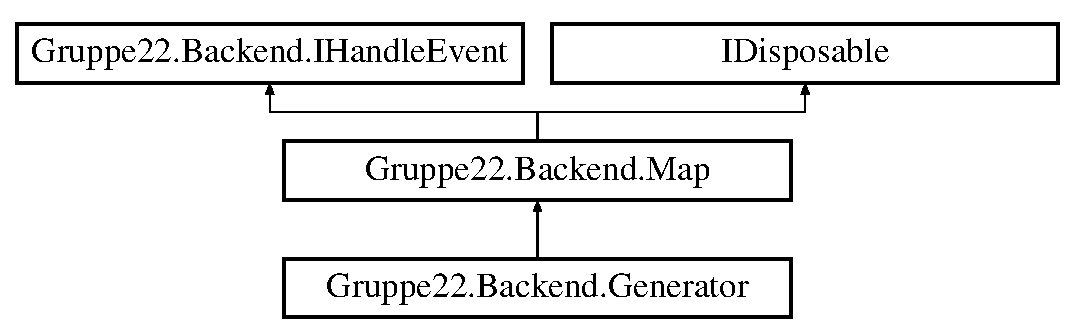
\includegraphics[height=3.000000cm]{class_gruppe22_1_1_backend_1_1_generator}
\end{center}
\end{figure}
\subsection*{Öffentliche Methoden}
\begin{DoxyCompactItemize}
\item 
void \hyperlink{class_gruppe22_1_1_backend_1_1_generator_ac8a9e00ddef47ce83f09a443bffed45a}{Add\-Stairs} (\hyperlink{class_gruppe22_1_1_backend_1_1_coords}{Coords} src\-Coords, int target\-Room, \hyperlink{class_gruppe22_1_1_backend_1_1_coords}{Backend.\-Coords} target\-Coords, bool up)
\item 
void \hyperlink{class_gruppe22_1_1_backend_1_1_generator_aea51f47ba3daf93d121cdd6b3f617d4f}{Add\-Player} (\hyperlink{class_gruppe22_1_1_backend_1_1_coords}{Coords} pos)
\item 
override void \hyperlink{class_gruppe22_1_1_backend_1_1_generator_ae0e94d668013ad78b8ed91f98009e488}{Save} (string filename)
\begin{DoxyCompactList}\small\item\em Write the current map to a file \end{DoxyCompactList}\item 
void \hyperlink{class_gruppe22_1_1_backend_1_1_generator_a538008c22b6442b950e50451ce575f91}{Add\-Enemies} (int amount=-\/1)
\item 
void \hyperlink{class_gruppe22_1_1_backend_1_1_generator_ae813499646756000d3288e683776d24d}{Add\-N\-P\-C} (int amount=-\/1)
\item 
void \hyperlink{class_gruppe22_1_1_backend_1_1_generator_a90af0ec184078329dae4f36205156f6a}{Add\-Boss} ()
\item 
void \hyperlink{class_gruppe22_1_1_backend_1_1_generator_a961803e6679ad31bc9305a35d4927a49}{Add\-Shop} ()
\item 
void \hyperlink{class_gruppe22_1_1_backend_1_1_generator_a3fc322786a2cc1680f500de2f664708c}{Add\-Checkpoint} ()
\item 
void \hyperlink{class_gruppe22_1_1_backend_1_1_generator_ad1c57acfaecff0f8810e57ff32c71685}{Add\-Target} (\hyperlink{class_gruppe22_1_1_backend_1_1_coords}{Coords} src\-Coords)
\item 
void \hyperlink{class_gruppe22_1_1_backend_1_1_generator_ab6dbb4455d4ab380f5951312ca52ee0b}{Add\-Doors} (int room\-I\-D=1, int max\-Room=3, List$<$ \hyperlink{class_gruppe22_1_1_backend_1_1_exit}{Exit} $>$ doors=null)
\item 
\hyperlink{class_gruppe22_1_1_backend_1_1_coords}{Backend.\-Coords} \hyperlink{class_gruppe22_1_1_backend_1_1_generator_a72c0d73906b5ca3fe948c47ce964b354}{Suggest\-Exit} (\hyperlink{namespace_gruppe22_1_1_backend_a2d53d5d14b8ea0951ba6971e5da1ebf5}{Direction} dir)
\begin{DoxyCompactList}\small\item\em Find an appropriate place to pu an exit on the map \end{DoxyCompactList}\item 
void \hyperlink{class_gruppe22_1_1_backend_1_1_generator_a7e557a786bf0c8f614e2bed0e8ce0b03}{Connect\-To} (\hyperlink{class_gruppe22_1_1_backend_1_1_coords}{Coords} from, int Room, \hyperlink{class_gruppe22_1_1_backend_1_1_coords}{Backend.\-Coords} to, bool is\-Teleport=false)
\begin{DoxyCompactList}\small\item\em Add a doorway / stairway / teleporter to another room \end{DoxyCompactList}\item 
bool \hyperlink{class_gruppe22_1_1_backend_1_1_generator_ad3051d8d64ac5daec66d91421bb6e8f7}{Has\-Exit} (\hyperlink{namespace_gruppe22_1_1_backend_a2d53d5d14b8ea0951ba6971e5da1ebf5}{Direction} dir)
\item 
void \hyperlink{class_gruppe22_1_1_backend_1_1_generator_af49f7aaeb8fb4933504e3ebcb08bd256}{Add\-Items} (int amount=-\/1)
\item 
void \hyperlink{class_gruppe22_1_1_backend_1_1_generator_a95e36a3fb9b9deb35eafa57dd59edfde}{Clear\-Walls} (int amount=-\/1)
\begin{DoxyCompactList}\small\item\em Remove walls at random for more space \end{DoxyCompactList}\item 
void \hyperlink{class_gruppe22_1_1_backend_1_1_generator_a838990f7ecc479132b02a77b1e860565}{Cleanup\-Room} ()
\item 
void \hyperlink{class_gruppe22_1_1_backend_1_1_generator_ad27fdd309bf3c11574ed191363ac5bc9}{Clear\-Maze} ()
\begin{DoxyCompactList}\small\item\em Create a grid of walls \end{DoxyCompactList}\item 
void \hyperlink{class_gruppe22_1_1_backend_1_1_generator_a589a71fc90afb530b6bd960878910643}{Add\-Traps} (int amount=-\/1)
\item 
void \hyperlink{class_gruppe22_1_1_backend_1_1_generator_ab4241a0099707a0d99ca475ac4d11b40}{Generate\-Maze} ()
\begin{DoxyCompactList}\small\item\em Create a new maze \end{DoxyCompactList}\item 
bool \hyperlink{class_gruppe22_1_1_backend_1_1_generator_a58536bf78efafe5a8dd9371ec21ede7d}{From\-String} (string input, int room\-I\-D, int Max\-Room)
\item 
\hyperlink{class_gruppe22_1_1_backend_1_1_generator_a8e8cfc06fe85ddb9bbd411d302c0ea9b}{Generator} (Content\-Manager content, object parent, string pattern, int room\-Nr=1, int max\-Room=3, List$<$ \hyperlink{class_gruppe22_1_1_backend_1_1_exit}{Exit} $>$ \hyperlink{class_gruppe22_1_1_backend_1_1_generator_a08c85796fec36eaf888e0c2d8af5cb64}{exits}=null, Random rnd=null)
\item 
void \hyperlink{class_gruppe22_1_1_backend_1_1_generator_a88a3cb0906939d17f3da6ec4de64d806}{Generate\-Dungeon} ()
\item 
void \hyperlink{class_gruppe22_1_1_backend_1_1_generator_a7bf9e6e47ab06d7170532fcf8973a4ce}{Generate\-Room\-Name} ()
\item 
void \hyperlink{class_gruppe22_1_1_backend_1_1_generator_abaad74e28f0f25b9abab6e9c22960bff}{Draw\-Walls} ()
\item 
\hyperlink{class_gruppe22_1_1_backend_1_1_generator_a83efc83dbd633e8f008a05df0dc45812}{Generator} (Content\-Manager content, object parent=null, int \hyperlink{class_gruppe22_1_1_backend_1_1_map_ae185d7c51dd35311f6065044e603e81f}{width}=10, int \hyperlink{class_gruppe22_1_1_backend_1_1_map_aef59f2269d64d10b35acbabb6461fa55}{height}=10, bool generate=false, \hyperlink{class_gruppe22_1_1_backend_1_1_coords}{Backend.\-Coords} player\-Pos=null, int room\-Nr=1, int max\-Room=3, Random rnd=null, string \hyperlink{class_gruppe22_1_1_backend_1_1_map_a76814bb49c2210b400230b9ee530010f}{dungeonname}=\char`\"{}\char`\"{}, int \hyperlink{class_gruppe22_1_1_backend_1_1_map_abf7263c43d22ca634eceba89c06904cf}{level}=0, bool has\-Shop=false, bool has\-N\-P\-C=false, bool has\-Boss=false)
\begin{DoxyCompactList}\small\item\em Create an empty map \end{DoxyCompactList}\end{DoxyCompactItemize}
\subsection*{Propertys}
\begin{DoxyCompactItemize}
\item 
bool \hyperlink{class_gruppe22_1_1_backend_1_1_generator_a78432433649cd8d0c4f2dc1c49c6821f}{connected}\hspace{0.3cm}{\ttfamily  \mbox{[}get, set\mbox{]}}
\item 
List$<$ int $>$ \hyperlink{class_gruppe22_1_1_backend_1_1_generator_a4d4db744aab453a9ad1317fc280f80a0}{connected\-Rooms}\hspace{0.3cm}{\ttfamily  \mbox{[}get\mbox{]}}
\item 
new \hyperlink{namespace_gruppe22_1_1_backend_a2d53d5d14b8ea0951ba6971e5da1ebf5}{Direction} \hyperlink{class_gruppe22_1_1_backend_1_1_generator_a08c85796fec36eaf888e0c2d8af5cb64}{exits}\hspace{0.3cm}{\ttfamily  \mbox{[}get\mbox{]}}
\item 
bool \hyperlink{class_gruppe22_1_1_backend_1_1_generator_acd434164e04bd866a5130d6333cc9b62}{has\-Stairs}\hspace{0.3cm}{\ttfamily  \mbox{[}get\mbox{]}}
\item 
\hyperlink{class_gruppe22_1_1_backend_1_1_coords}{Backend.\-Coords} \hyperlink{class_gruppe22_1_1_backend_1_1_generator_a906ef2c015d9023394368b450dabbcdc}{Find\-Room\-For\-Stairs}\hspace{0.3cm}{\ttfamily  \mbox{[}get\mbox{]}}
\item 
\hyperlink{namespace_gruppe22_1_1_backend_a2d53d5d14b8ea0951ba6971e5da1ebf5}{Direction} \hyperlink{class_gruppe22_1_1_backend_1_1_generator_ae8a5091874b204ac692ce85ec56b495a}{blocked}\hspace{0.3cm}{\ttfamily  \mbox{[}get\mbox{]}}
\end{DoxyCompactItemize}
\subsection*{Weitere Geerbte Elemente}


\subsection{Beschreibung der Konstruktoren und Destruktoren}
\hypertarget{class_gruppe22_1_1_backend_1_1_generator_a8e8cfc06fe85ddb9bbd411d302c0ea9b}{\index{Gruppe22\-::\-Backend\-::\-Generator@{Gruppe22\-::\-Backend\-::\-Generator}!Generator@{Generator}}
\index{Generator@{Generator}!Gruppe22::Backend::Generator@{Gruppe22\-::\-Backend\-::\-Generator}}
\subsubsection[{Generator}]{\setlength{\rightskip}{0pt plus 5cm}Gruppe22.\-Backend.\-Generator.\-Generator (
\begin{DoxyParamCaption}
\item[{Content\-Manager}]{content, }
\item[{object}]{parent, }
\item[{string}]{pattern, }
\item[{int}]{room\-Nr = {\ttfamily 1}, }
\item[{int}]{max\-Room = {\ttfamily 3}, }
\item[{List$<$ {\bf Exit} $>$}]{exits = {\ttfamily null}, }
\item[{Random}]{rnd = {\ttfamily null}}
\end{DoxyParamCaption}
)}}\label{class_gruppe22_1_1_backend_1_1_generator_a8e8cfc06fe85ddb9bbd411d302c0ea9b}
\hypertarget{class_gruppe22_1_1_backend_1_1_generator_a83efc83dbd633e8f008a05df0dc45812}{\index{Gruppe22\-::\-Backend\-::\-Generator@{Gruppe22\-::\-Backend\-::\-Generator}!Generator@{Generator}}
\index{Generator@{Generator}!Gruppe22::Backend::Generator@{Gruppe22\-::\-Backend\-::\-Generator}}
\subsubsection[{Generator}]{\setlength{\rightskip}{0pt plus 5cm}Gruppe22.\-Backend.\-Generator.\-Generator (
\begin{DoxyParamCaption}
\item[{Content\-Manager}]{content, }
\item[{object}]{parent = {\ttfamily null}, }
\item[{int}]{width = {\ttfamily 10}, }
\item[{int}]{height = {\ttfamily 10}, }
\item[{bool}]{generate = {\ttfamily false}, }
\item[{{\bf Backend.\-Coords}}]{player\-Pos = {\ttfamily null}, }
\item[{int}]{room\-Nr = {\ttfamily 1}, }
\item[{int}]{max\-Room = {\ttfamily 3}, }
\item[{Random}]{rnd = {\ttfamily null}, }
\item[{string}]{dungeonname = {\ttfamily \char`\"{}\char`\"{}}, }
\item[{int}]{level = {\ttfamily 0}, }
\item[{bool}]{has\-Shop = {\ttfamily false}, }
\item[{bool}]{has\-N\-P\-C = {\ttfamily false}, }
\item[{bool}]{has\-Boss = {\ttfamily false}}
\end{DoxyParamCaption}
)}}\label{class_gruppe22_1_1_backend_1_1_generator_a83efc83dbd633e8f008a05df0dc45812}


Create an empty map 


\begin{DoxyParams}{Parameter}
{\em width} & The width of the map\\
\hline
{\em height} & The height of the map\\
\hline
\end{DoxyParams}


\subsection{Dokumentation der Elementfunktionen}
\hypertarget{class_gruppe22_1_1_backend_1_1_generator_a90af0ec184078329dae4f36205156f6a}{\index{Gruppe22\-::\-Backend\-::\-Generator@{Gruppe22\-::\-Backend\-::\-Generator}!Add\-Boss@{Add\-Boss}}
\index{Add\-Boss@{Add\-Boss}!Gruppe22::Backend::Generator@{Gruppe22\-::\-Backend\-::\-Generator}}
\subsubsection[{Add\-Boss}]{\setlength{\rightskip}{0pt plus 5cm}void Gruppe22.\-Backend.\-Generator.\-Add\-Boss (
\begin{DoxyParamCaption}
{}
\end{DoxyParamCaption}
)}}\label{class_gruppe22_1_1_backend_1_1_generator_a90af0ec184078329dae4f36205156f6a}
\hypertarget{class_gruppe22_1_1_backend_1_1_generator_a3fc322786a2cc1680f500de2f664708c}{\index{Gruppe22\-::\-Backend\-::\-Generator@{Gruppe22\-::\-Backend\-::\-Generator}!Add\-Checkpoint@{Add\-Checkpoint}}
\index{Add\-Checkpoint@{Add\-Checkpoint}!Gruppe22::Backend::Generator@{Gruppe22\-::\-Backend\-::\-Generator}}
\subsubsection[{Add\-Checkpoint}]{\setlength{\rightskip}{0pt plus 5cm}void Gruppe22.\-Backend.\-Generator.\-Add\-Checkpoint (
\begin{DoxyParamCaption}
{}
\end{DoxyParamCaption}
)}}\label{class_gruppe22_1_1_backend_1_1_generator_a3fc322786a2cc1680f500de2f664708c}
\hypertarget{class_gruppe22_1_1_backend_1_1_generator_ab6dbb4455d4ab380f5951312ca52ee0b}{\index{Gruppe22\-::\-Backend\-::\-Generator@{Gruppe22\-::\-Backend\-::\-Generator}!Add\-Doors@{Add\-Doors}}
\index{Add\-Doors@{Add\-Doors}!Gruppe22::Backend::Generator@{Gruppe22\-::\-Backend\-::\-Generator}}
\subsubsection[{Add\-Doors}]{\setlength{\rightskip}{0pt plus 5cm}void Gruppe22.\-Backend.\-Generator.\-Add\-Doors (
\begin{DoxyParamCaption}
\item[{int}]{room\-I\-D = {\ttfamily 1}, }
\item[{int}]{max\-Room = {\ttfamily 3}, }
\item[{List$<$ {\bf Exit} $>$}]{doors = {\ttfamily null}}
\end{DoxyParamCaption}
)}}\label{class_gruppe22_1_1_backend_1_1_generator_ab6dbb4455d4ab380f5951312ca52ee0b}
\hypertarget{class_gruppe22_1_1_backend_1_1_generator_a538008c22b6442b950e50451ce575f91}{\index{Gruppe22\-::\-Backend\-::\-Generator@{Gruppe22\-::\-Backend\-::\-Generator}!Add\-Enemies@{Add\-Enemies}}
\index{Add\-Enemies@{Add\-Enemies}!Gruppe22::Backend::Generator@{Gruppe22\-::\-Backend\-::\-Generator}}
\subsubsection[{Add\-Enemies}]{\setlength{\rightskip}{0pt plus 5cm}void Gruppe22.\-Backend.\-Generator.\-Add\-Enemies (
\begin{DoxyParamCaption}
\item[{int}]{amount = {\ttfamily -\/1}}
\end{DoxyParamCaption}
)}}\label{class_gruppe22_1_1_backend_1_1_generator_a538008c22b6442b950e50451ce575f91}
\hypertarget{class_gruppe22_1_1_backend_1_1_generator_af49f7aaeb8fb4933504e3ebcb08bd256}{\index{Gruppe22\-::\-Backend\-::\-Generator@{Gruppe22\-::\-Backend\-::\-Generator}!Add\-Items@{Add\-Items}}
\index{Add\-Items@{Add\-Items}!Gruppe22::Backend::Generator@{Gruppe22\-::\-Backend\-::\-Generator}}
\subsubsection[{Add\-Items}]{\setlength{\rightskip}{0pt plus 5cm}void Gruppe22.\-Backend.\-Generator.\-Add\-Items (
\begin{DoxyParamCaption}
\item[{int}]{amount = {\ttfamily -\/1}}
\end{DoxyParamCaption}
)}}\label{class_gruppe22_1_1_backend_1_1_generator_af49f7aaeb8fb4933504e3ebcb08bd256}
\hypertarget{class_gruppe22_1_1_backend_1_1_generator_ae813499646756000d3288e683776d24d}{\index{Gruppe22\-::\-Backend\-::\-Generator@{Gruppe22\-::\-Backend\-::\-Generator}!Add\-N\-P\-C@{Add\-N\-P\-C}}
\index{Add\-N\-P\-C@{Add\-N\-P\-C}!Gruppe22::Backend::Generator@{Gruppe22\-::\-Backend\-::\-Generator}}
\subsubsection[{Add\-N\-P\-C}]{\setlength{\rightskip}{0pt plus 5cm}void Gruppe22.\-Backend.\-Generator.\-Add\-N\-P\-C (
\begin{DoxyParamCaption}
\item[{int}]{amount = {\ttfamily -\/1}}
\end{DoxyParamCaption}
)}}\label{class_gruppe22_1_1_backend_1_1_generator_ae813499646756000d3288e683776d24d}
\hypertarget{class_gruppe22_1_1_backend_1_1_generator_aea51f47ba3daf93d121cdd6b3f617d4f}{\index{Gruppe22\-::\-Backend\-::\-Generator@{Gruppe22\-::\-Backend\-::\-Generator}!Add\-Player@{Add\-Player}}
\index{Add\-Player@{Add\-Player}!Gruppe22::Backend::Generator@{Gruppe22\-::\-Backend\-::\-Generator}}
\subsubsection[{Add\-Player}]{\setlength{\rightskip}{0pt plus 5cm}void Gruppe22.\-Backend.\-Generator.\-Add\-Player (
\begin{DoxyParamCaption}
\item[{{\bf Coords}}]{pos}
\end{DoxyParamCaption}
)}}\label{class_gruppe22_1_1_backend_1_1_generator_aea51f47ba3daf93d121cdd6b3f617d4f}
\hypertarget{class_gruppe22_1_1_backend_1_1_generator_a961803e6679ad31bc9305a35d4927a49}{\index{Gruppe22\-::\-Backend\-::\-Generator@{Gruppe22\-::\-Backend\-::\-Generator}!Add\-Shop@{Add\-Shop}}
\index{Add\-Shop@{Add\-Shop}!Gruppe22::Backend::Generator@{Gruppe22\-::\-Backend\-::\-Generator}}
\subsubsection[{Add\-Shop}]{\setlength{\rightskip}{0pt plus 5cm}void Gruppe22.\-Backend.\-Generator.\-Add\-Shop (
\begin{DoxyParamCaption}
{}
\end{DoxyParamCaption}
)}}\label{class_gruppe22_1_1_backend_1_1_generator_a961803e6679ad31bc9305a35d4927a49}
\hypertarget{class_gruppe22_1_1_backend_1_1_generator_ac8a9e00ddef47ce83f09a443bffed45a}{\index{Gruppe22\-::\-Backend\-::\-Generator@{Gruppe22\-::\-Backend\-::\-Generator}!Add\-Stairs@{Add\-Stairs}}
\index{Add\-Stairs@{Add\-Stairs}!Gruppe22::Backend::Generator@{Gruppe22\-::\-Backend\-::\-Generator}}
\subsubsection[{Add\-Stairs}]{\setlength{\rightskip}{0pt plus 5cm}void Gruppe22.\-Backend.\-Generator.\-Add\-Stairs (
\begin{DoxyParamCaption}
\item[{{\bf Coords}}]{src\-Coords, }
\item[{int}]{target\-Room, }
\item[{{\bf Backend.\-Coords}}]{target\-Coords, }
\item[{bool}]{up}
\end{DoxyParamCaption}
)}}\label{class_gruppe22_1_1_backend_1_1_generator_ac8a9e00ddef47ce83f09a443bffed45a}
\hypertarget{class_gruppe22_1_1_backend_1_1_generator_ad1c57acfaecff0f8810e57ff32c71685}{\index{Gruppe22\-::\-Backend\-::\-Generator@{Gruppe22\-::\-Backend\-::\-Generator}!Add\-Target@{Add\-Target}}
\index{Add\-Target@{Add\-Target}!Gruppe22::Backend::Generator@{Gruppe22\-::\-Backend\-::\-Generator}}
\subsubsection[{Add\-Target}]{\setlength{\rightskip}{0pt plus 5cm}void Gruppe22.\-Backend.\-Generator.\-Add\-Target (
\begin{DoxyParamCaption}
\item[{{\bf Coords}}]{src\-Coords}
\end{DoxyParamCaption}
)}}\label{class_gruppe22_1_1_backend_1_1_generator_ad1c57acfaecff0f8810e57ff32c71685}
\hypertarget{class_gruppe22_1_1_backend_1_1_generator_a589a71fc90afb530b6bd960878910643}{\index{Gruppe22\-::\-Backend\-::\-Generator@{Gruppe22\-::\-Backend\-::\-Generator}!Add\-Traps@{Add\-Traps}}
\index{Add\-Traps@{Add\-Traps}!Gruppe22::Backend::Generator@{Gruppe22\-::\-Backend\-::\-Generator}}
\subsubsection[{Add\-Traps}]{\setlength{\rightskip}{0pt plus 5cm}void Gruppe22.\-Backend.\-Generator.\-Add\-Traps (
\begin{DoxyParamCaption}
\item[{int}]{amount = {\ttfamily -\/1}}
\end{DoxyParamCaption}
)}}\label{class_gruppe22_1_1_backend_1_1_generator_a589a71fc90afb530b6bd960878910643}
\hypertarget{class_gruppe22_1_1_backend_1_1_generator_a838990f7ecc479132b02a77b1e860565}{\index{Gruppe22\-::\-Backend\-::\-Generator@{Gruppe22\-::\-Backend\-::\-Generator}!Cleanup\-Room@{Cleanup\-Room}}
\index{Cleanup\-Room@{Cleanup\-Room}!Gruppe22::Backend::Generator@{Gruppe22\-::\-Backend\-::\-Generator}}
\subsubsection[{Cleanup\-Room}]{\setlength{\rightskip}{0pt plus 5cm}void Gruppe22.\-Backend.\-Generator.\-Cleanup\-Room (
\begin{DoxyParamCaption}
{}
\end{DoxyParamCaption}
)}}\label{class_gruppe22_1_1_backend_1_1_generator_a838990f7ecc479132b02a77b1e860565}
\hypertarget{class_gruppe22_1_1_backend_1_1_generator_ad27fdd309bf3c11574ed191363ac5bc9}{\index{Gruppe22\-::\-Backend\-::\-Generator@{Gruppe22\-::\-Backend\-::\-Generator}!Clear\-Maze@{Clear\-Maze}}
\index{Clear\-Maze@{Clear\-Maze}!Gruppe22::Backend::Generator@{Gruppe22\-::\-Backend\-::\-Generator}}
\subsubsection[{Clear\-Maze}]{\setlength{\rightskip}{0pt plus 5cm}void Gruppe22.\-Backend.\-Generator.\-Clear\-Maze (
\begin{DoxyParamCaption}
{}
\end{DoxyParamCaption}
)}}\label{class_gruppe22_1_1_backend_1_1_generator_ad27fdd309bf3c11574ed191363ac5bc9}


Create a grid of walls 

\hypertarget{class_gruppe22_1_1_backend_1_1_generator_a95e36a3fb9b9deb35eafa57dd59edfde}{\index{Gruppe22\-::\-Backend\-::\-Generator@{Gruppe22\-::\-Backend\-::\-Generator}!Clear\-Walls@{Clear\-Walls}}
\index{Clear\-Walls@{Clear\-Walls}!Gruppe22::Backend::Generator@{Gruppe22\-::\-Backend\-::\-Generator}}
\subsubsection[{Clear\-Walls}]{\setlength{\rightskip}{0pt plus 5cm}void Gruppe22.\-Backend.\-Generator.\-Clear\-Walls (
\begin{DoxyParamCaption}
\item[{int}]{amount = {\ttfamily -\/1}}
\end{DoxyParamCaption}
)}}\label{class_gruppe22_1_1_backend_1_1_generator_a95e36a3fb9b9deb35eafa57dd59edfde}


Remove walls at random for more space 


\begin{DoxyParams}{Parameter}
{\em amount} & Amount of walls to remove\\
\hline
\end{DoxyParams}
\hypertarget{class_gruppe22_1_1_backend_1_1_generator_a7e557a786bf0c8f614e2bed0e8ce0b03}{\index{Gruppe22\-::\-Backend\-::\-Generator@{Gruppe22\-::\-Backend\-::\-Generator}!Connect\-To@{Connect\-To}}
\index{Connect\-To@{Connect\-To}!Gruppe22::Backend::Generator@{Gruppe22\-::\-Backend\-::\-Generator}}
\subsubsection[{Connect\-To}]{\setlength{\rightskip}{0pt plus 5cm}void Gruppe22.\-Backend.\-Generator.\-Connect\-To (
\begin{DoxyParamCaption}
\item[{{\bf Coords}}]{from, }
\item[{int}]{Room, }
\item[{{\bf Backend.\-Coords}}]{to, }
\item[{bool}]{is\-Teleport = {\ttfamily false}}
\end{DoxyParamCaption}
)}}\label{class_gruppe22_1_1_backend_1_1_generator_a7e557a786bf0c8f614e2bed0e8ce0b03}


Add a doorway / stairway / teleporter to another room 


\begin{DoxyParams}{Parameter}
{\em from} & Coordinates in this room\\
\hline
{\em Room} & Uinque I\-D of target room\\
\hline
{\em to} & Coordinates in target room\\
\hline
\end{DoxyParams}
\hypertarget{class_gruppe22_1_1_backend_1_1_generator_abaad74e28f0f25b9abab6e9c22960bff}{\index{Gruppe22\-::\-Backend\-::\-Generator@{Gruppe22\-::\-Backend\-::\-Generator}!Draw\-Walls@{Draw\-Walls}}
\index{Draw\-Walls@{Draw\-Walls}!Gruppe22::Backend::Generator@{Gruppe22\-::\-Backend\-::\-Generator}}
\subsubsection[{Draw\-Walls}]{\setlength{\rightskip}{0pt plus 5cm}void Gruppe22.\-Backend.\-Generator.\-Draw\-Walls (
\begin{DoxyParamCaption}
{}
\end{DoxyParamCaption}
)}}\label{class_gruppe22_1_1_backend_1_1_generator_abaad74e28f0f25b9abab6e9c22960bff}
\hypertarget{class_gruppe22_1_1_backend_1_1_generator_a58536bf78efafe5a8dd9371ec21ede7d}{\index{Gruppe22\-::\-Backend\-::\-Generator@{Gruppe22\-::\-Backend\-::\-Generator}!From\-String@{From\-String}}
\index{From\-String@{From\-String}!Gruppe22::Backend::Generator@{Gruppe22\-::\-Backend\-::\-Generator}}
\subsubsection[{From\-String}]{\setlength{\rightskip}{0pt plus 5cm}bool Gruppe22.\-Backend.\-Generator.\-From\-String (
\begin{DoxyParamCaption}
\item[{string}]{input, }
\item[{int}]{room\-I\-D, }
\item[{int}]{Max\-Room}
\end{DoxyParamCaption}
)}}\label{class_gruppe22_1_1_backend_1_1_generator_a58536bf78efafe5a8dd9371ec21ede7d}
\hypertarget{class_gruppe22_1_1_backend_1_1_generator_a88a3cb0906939d17f3da6ec4de64d806}{\index{Gruppe22\-::\-Backend\-::\-Generator@{Gruppe22\-::\-Backend\-::\-Generator}!Generate\-Dungeon@{Generate\-Dungeon}}
\index{Generate\-Dungeon@{Generate\-Dungeon}!Gruppe22::Backend::Generator@{Gruppe22\-::\-Backend\-::\-Generator}}
\subsubsection[{Generate\-Dungeon}]{\setlength{\rightskip}{0pt plus 5cm}void Gruppe22.\-Backend.\-Generator.\-Generate\-Dungeon (
\begin{DoxyParamCaption}
{}
\end{DoxyParamCaption}
)}}\label{class_gruppe22_1_1_backend_1_1_generator_a88a3cb0906939d17f3da6ec4de64d806}
\hypertarget{class_gruppe22_1_1_backend_1_1_generator_ab4241a0099707a0d99ca475ac4d11b40}{\index{Gruppe22\-::\-Backend\-::\-Generator@{Gruppe22\-::\-Backend\-::\-Generator}!Generate\-Maze@{Generate\-Maze}}
\index{Generate\-Maze@{Generate\-Maze}!Gruppe22::Backend::Generator@{Gruppe22\-::\-Backend\-::\-Generator}}
\subsubsection[{Generate\-Maze}]{\setlength{\rightskip}{0pt plus 5cm}void Gruppe22.\-Backend.\-Generator.\-Generate\-Maze (
\begin{DoxyParamCaption}
{}
\end{DoxyParamCaption}
)}}\label{class_gruppe22_1_1_backend_1_1_generator_ab4241a0099707a0d99ca475ac4d11b40}


Create a new maze 


\begin{DoxyParams}{Parameter}
{\em slow} & \\
\hline
\end{DoxyParams}
\hypertarget{class_gruppe22_1_1_backend_1_1_generator_a7bf9e6e47ab06d7170532fcf8973a4ce}{\index{Gruppe22\-::\-Backend\-::\-Generator@{Gruppe22\-::\-Backend\-::\-Generator}!Generate\-Room\-Name@{Generate\-Room\-Name}}
\index{Generate\-Room\-Name@{Generate\-Room\-Name}!Gruppe22::Backend::Generator@{Gruppe22\-::\-Backend\-::\-Generator}}
\subsubsection[{Generate\-Room\-Name}]{\setlength{\rightskip}{0pt plus 5cm}void Gruppe22.\-Backend.\-Generator.\-Generate\-Room\-Name (
\begin{DoxyParamCaption}
{}
\end{DoxyParamCaption}
)}}\label{class_gruppe22_1_1_backend_1_1_generator_a7bf9e6e47ab06d7170532fcf8973a4ce}
\hypertarget{class_gruppe22_1_1_backend_1_1_generator_ad3051d8d64ac5daec66d91421bb6e8f7}{\index{Gruppe22\-::\-Backend\-::\-Generator@{Gruppe22\-::\-Backend\-::\-Generator}!Has\-Exit@{Has\-Exit}}
\index{Has\-Exit@{Has\-Exit}!Gruppe22::Backend::Generator@{Gruppe22\-::\-Backend\-::\-Generator}}
\subsubsection[{Has\-Exit}]{\setlength{\rightskip}{0pt plus 5cm}bool Gruppe22.\-Backend.\-Generator.\-Has\-Exit (
\begin{DoxyParamCaption}
\item[{{\bf Direction}}]{dir}
\end{DoxyParamCaption}
)}}\label{class_gruppe22_1_1_backend_1_1_generator_ad3051d8d64ac5daec66d91421bb6e8f7}
\hypertarget{class_gruppe22_1_1_backend_1_1_generator_ae0e94d668013ad78b8ed91f98009e488}{\index{Gruppe22\-::\-Backend\-::\-Generator@{Gruppe22\-::\-Backend\-::\-Generator}!Save@{Save}}
\index{Save@{Save}!Gruppe22::Backend::Generator@{Gruppe22\-::\-Backend\-::\-Generator}}
\subsubsection[{Save}]{\setlength{\rightskip}{0pt plus 5cm}override void Gruppe22.\-Backend.\-Generator.\-Save (
\begin{DoxyParamCaption}
\item[{string}]{filename}
\end{DoxyParamCaption}
)\hspace{0.3cm}{\ttfamily [virtual]}}}\label{class_gruppe22_1_1_backend_1_1_generator_ae0e94d668013ad78b8ed91f98009e488}


Write the current map to a file 


\begin{DoxyParams}{Parameter}
{\em filename} & The filename to write to\\
\hline
\end{DoxyParams}
\begin{DoxyReturn}{Rückgabe}
true if writing was successful
\end{DoxyReturn}


Erneute Implementation von \hyperlink{class_gruppe22_1_1_backend_1_1_map_ab1fe0990776579437497c699222253db}{Gruppe22.\-Backend.\-Map}.

\hypertarget{class_gruppe22_1_1_backend_1_1_generator_a72c0d73906b5ca3fe948c47ce964b354}{\index{Gruppe22\-::\-Backend\-::\-Generator@{Gruppe22\-::\-Backend\-::\-Generator}!Suggest\-Exit@{Suggest\-Exit}}
\index{Suggest\-Exit@{Suggest\-Exit}!Gruppe22::Backend::Generator@{Gruppe22\-::\-Backend\-::\-Generator}}
\subsubsection[{Suggest\-Exit}]{\setlength{\rightskip}{0pt plus 5cm}{\bf Backend.\-Coords} Gruppe22.\-Backend.\-Generator.\-Suggest\-Exit (
\begin{DoxyParamCaption}
\item[{{\bf Direction}}]{dir}
\end{DoxyParamCaption}
)}}\label{class_gruppe22_1_1_backend_1_1_generator_a72c0d73906b5ca3fe948c47ce964b354}


Find an appropriate place to pu an exit on the map 


\begin{DoxyParams}{Parameter}
{\em dir} & Wall on which exit should be placed\\
\hline
\end{DoxyParams}
\begin{DoxyReturn}{Rückgabe}
Coordinates of the exit
\end{DoxyReturn}


\subsection{Dokumentation der Propertys}
\hypertarget{class_gruppe22_1_1_backend_1_1_generator_ae8a5091874b204ac692ce85ec56b495a}{\index{Gruppe22\-::\-Backend\-::\-Generator@{Gruppe22\-::\-Backend\-::\-Generator}!blocked@{blocked}}
\index{blocked@{blocked}!Gruppe22::Backend::Generator@{Gruppe22\-::\-Backend\-::\-Generator}}
\subsubsection[{blocked}]{\setlength{\rightskip}{0pt plus 5cm}{\bf Direction} Gruppe22.\-Backend.\-Generator.\-blocked\hspace{0.3cm}{\ttfamily [get]}}}\label{class_gruppe22_1_1_backend_1_1_generator_ae8a5091874b204ac692ce85ec56b495a}
\hypertarget{class_gruppe22_1_1_backend_1_1_generator_a78432433649cd8d0c4f2dc1c49c6821f}{\index{Gruppe22\-::\-Backend\-::\-Generator@{Gruppe22\-::\-Backend\-::\-Generator}!connected@{connected}}
\index{connected@{connected}!Gruppe22::Backend::Generator@{Gruppe22\-::\-Backend\-::\-Generator}}
\subsubsection[{connected}]{\setlength{\rightskip}{0pt plus 5cm}bool Gruppe22.\-Backend.\-Generator.\-connected\hspace{0.3cm}{\ttfamily [get]}, {\ttfamily [set]}}}\label{class_gruppe22_1_1_backend_1_1_generator_a78432433649cd8d0c4f2dc1c49c6821f}
\hypertarget{class_gruppe22_1_1_backend_1_1_generator_a4d4db744aab453a9ad1317fc280f80a0}{\index{Gruppe22\-::\-Backend\-::\-Generator@{Gruppe22\-::\-Backend\-::\-Generator}!connected\-Rooms@{connected\-Rooms}}
\index{connected\-Rooms@{connected\-Rooms}!Gruppe22::Backend::Generator@{Gruppe22\-::\-Backend\-::\-Generator}}
\subsubsection[{connected\-Rooms}]{\setlength{\rightskip}{0pt plus 5cm}List$<$int$>$ Gruppe22.\-Backend.\-Generator.\-connected\-Rooms\hspace{0.3cm}{\ttfamily [get]}}}\label{class_gruppe22_1_1_backend_1_1_generator_a4d4db744aab453a9ad1317fc280f80a0}
\hypertarget{class_gruppe22_1_1_backend_1_1_generator_a08c85796fec36eaf888e0c2d8af5cb64}{\index{Gruppe22\-::\-Backend\-::\-Generator@{Gruppe22\-::\-Backend\-::\-Generator}!exits@{exits}}
\index{exits@{exits}!Gruppe22::Backend::Generator@{Gruppe22\-::\-Backend\-::\-Generator}}
\subsubsection[{exits}]{\setlength{\rightskip}{0pt plus 5cm}new {\bf Direction} Gruppe22.\-Backend.\-Generator.\-exits\hspace{0.3cm}{\ttfamily [get]}}}\label{class_gruppe22_1_1_backend_1_1_generator_a08c85796fec36eaf888e0c2d8af5cb64}
\hypertarget{class_gruppe22_1_1_backend_1_1_generator_a906ef2c015d9023394368b450dabbcdc}{\index{Gruppe22\-::\-Backend\-::\-Generator@{Gruppe22\-::\-Backend\-::\-Generator}!Find\-Room\-For\-Stairs@{Find\-Room\-For\-Stairs}}
\index{Find\-Room\-For\-Stairs@{Find\-Room\-For\-Stairs}!Gruppe22::Backend::Generator@{Gruppe22\-::\-Backend\-::\-Generator}}
\subsubsection[{Find\-Room\-For\-Stairs}]{\setlength{\rightskip}{0pt plus 5cm}{\bf Backend.\-Coords} Gruppe22.\-Backend.\-Generator.\-Find\-Room\-For\-Stairs\hspace{0.3cm}{\ttfamily [get]}}}\label{class_gruppe22_1_1_backend_1_1_generator_a906ef2c015d9023394368b450dabbcdc}
\hypertarget{class_gruppe22_1_1_backend_1_1_generator_acd434164e04bd866a5130d6333cc9b62}{\index{Gruppe22\-::\-Backend\-::\-Generator@{Gruppe22\-::\-Backend\-::\-Generator}!has\-Stairs@{has\-Stairs}}
\index{has\-Stairs@{has\-Stairs}!Gruppe22::Backend::Generator@{Gruppe22\-::\-Backend\-::\-Generator}}
\subsubsection[{has\-Stairs}]{\setlength{\rightskip}{0pt plus 5cm}bool Gruppe22.\-Backend.\-Generator.\-has\-Stairs\hspace{0.3cm}{\ttfamily [get]}}}\label{class_gruppe22_1_1_backend_1_1_generator_acd434164e04bd866a5130d6333cc9b62}


Die Dokumentation für diese Klasse wurde erzeugt aufgrund der Datei\-:\begin{DoxyCompactItemize}
\item 
C\-:/\-Users/beursken/\-Documents/\-Git\-Hub/gruppe22/\-Gruppe22/\-Gruppe22/\-Backend/\-Map/\hyperlink{_generator_8cs}{Generator.\-cs}\end{DoxyCompactItemize}

\hypertarget{class_gruppe22_1_1_backend_1_1_generator_tile}{\section{Gruppe22.\-Backend.\-Generator\-Tile Klassenreferenz}
\label{class_gruppe22_1_1_backend_1_1_generator_tile}\index{Gruppe22.\-Backend.\-Generator\-Tile@{Gruppe22.\-Backend.\-Generator\-Tile}}
}
Klassendiagramm für Gruppe22.\-Backend.\-Generator\-Tile\-:\begin{figure}[H]
\begin{center}
\leavevmode
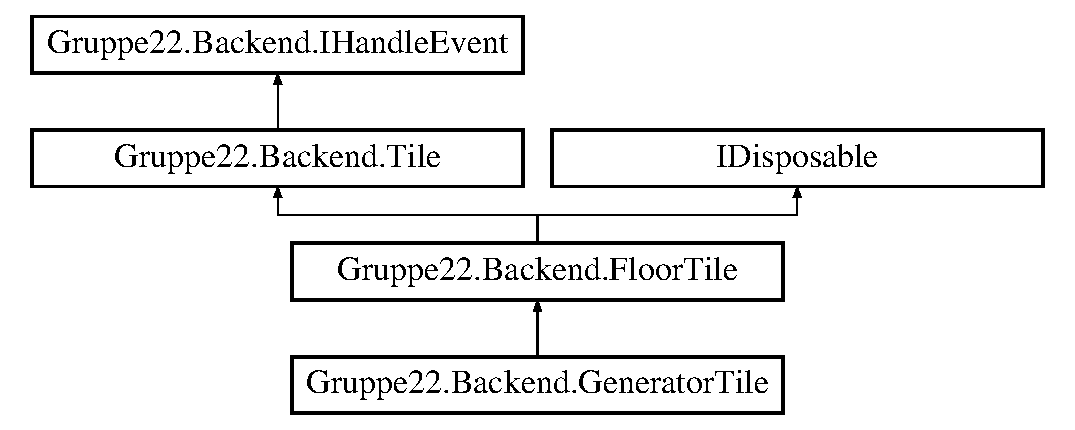
\includegraphics[height=4.000000cm]{class_gruppe22_1_1_backend_1_1_generator_tile}
\end{center}
\end{figure}
\subsection*{Öffentliche Methoden}
\begin{DoxyCompactItemize}
\item 
\hyperlink{class_gruppe22_1_1_backend_1_1_generator_tile_ab9314b37ebdeb42982a0eb130118729f}{Generator\-Tile} (object \hyperlink{class_gruppe22_1_1_backend_1_1_tile_abc12933c70eb3a2ebbb2fde9f45c2632}{parent})
\item 
\hyperlink{class_gruppe22_1_1_backend_1_1_generator_tile_a58aa521b8a1fa31e489c970d43f5a6c1}{Generator\-Tile} (object \hyperlink{class_gruppe22_1_1_backend_1_1_tile_abc12933c70eb3a2ebbb2fde9f45c2632}{parent}, \hyperlink{class_gruppe22_1_1_backend_1_1_coords}{Backend.\-Coords} \hyperlink{class_gruppe22_1_1_backend_1_1_floor_tile_a222af0c5d8ea6b7d24d04a384f71d70b}{coords}, bool \hyperlink{class_gruppe22_1_1_backend_1_1_floor_tile_a07516e27f9669dd9e852cf42a1a94635}{can\-Enter}, Random r)
\begin{DoxyCompactList}\small\item\em An empty constructor (setting default values) \end{DoxyCompactList}\end{DoxyCompactItemize}
\subsection*{Geschützte Attribute}
\begin{DoxyCompactItemize}
\item 
bool \hyperlink{class_gruppe22_1_1_backend_1_1_generator_tile_ada6c954a36d01b4d1df4bb616df9d3fb}{\-\_\-connected} = false
\begin{DoxyCompactList}\small\item\em Used by map generator (determines whether tile can be reached from at least one other tile \end{DoxyCompactList}\item 
\hyperlink{namespace_gruppe22_1_1_backend_a74373668761d179b11ba50e5980a8674}{Connection} \hyperlink{class_gruppe22_1_1_backend_1_1_generator_tile_ac32f05dfbc85524404f187d9235ae982}{\-\_\-connection} = Connection.\-Invalid
\begin{DoxyCompactList}\small\item\em Direction of connection \end{DoxyCompactList}\end{DoxyCompactItemize}
\subsection*{Propertys}
\begin{DoxyCompactItemize}
\item 
bool \hyperlink{class_gruppe22_1_1_backend_1_1_generator_tile_aa2f02c266ad7b74d788e669c9478d445}{connected}\hspace{0.3cm}{\ttfamily  \mbox{[}get, set\mbox{]}}
\item 
\hyperlink{namespace_gruppe22_1_1_backend_a74373668761d179b11ba50e5980a8674}{Connection} \hyperlink{class_gruppe22_1_1_backend_1_1_generator_tile_aae87ad2fa7e0b2903c73b2cd939b3637}{connection}\hspace{0.3cm}{\ttfamily  \mbox{[}get, set\mbox{]}}
\end{DoxyCompactItemize}


\subsection{Beschreibung der Konstruktoren und Destruktoren}
\hypertarget{class_gruppe22_1_1_backend_1_1_generator_tile_ab9314b37ebdeb42982a0eb130118729f}{\index{Gruppe22\-::\-Backend\-::\-Generator\-Tile@{Gruppe22\-::\-Backend\-::\-Generator\-Tile}!Generator\-Tile@{Generator\-Tile}}
\index{Generator\-Tile@{Generator\-Tile}!Gruppe22::Backend::GeneratorTile@{Gruppe22\-::\-Backend\-::\-Generator\-Tile}}
\subsubsection[{Generator\-Tile}]{\setlength{\rightskip}{0pt plus 5cm}Gruppe22.\-Backend.\-Generator\-Tile.\-Generator\-Tile (
\begin{DoxyParamCaption}
\item[{object}]{parent}
\end{DoxyParamCaption}
)}}\label{class_gruppe22_1_1_backend_1_1_generator_tile_ab9314b37ebdeb42982a0eb130118729f}
\hypertarget{class_gruppe22_1_1_backend_1_1_generator_tile_a58aa521b8a1fa31e489c970d43f5a6c1}{\index{Gruppe22\-::\-Backend\-::\-Generator\-Tile@{Gruppe22\-::\-Backend\-::\-Generator\-Tile}!Generator\-Tile@{Generator\-Tile}}
\index{Generator\-Tile@{Generator\-Tile}!Gruppe22::Backend::GeneratorTile@{Gruppe22\-::\-Backend\-::\-Generator\-Tile}}
\subsubsection[{Generator\-Tile}]{\setlength{\rightskip}{0pt plus 5cm}Gruppe22.\-Backend.\-Generator\-Tile.\-Generator\-Tile (
\begin{DoxyParamCaption}
\item[{object}]{parent, }
\item[{{\bf Backend.\-Coords}}]{coords, }
\item[{bool}]{can\-Enter, }
\item[{Random}]{r}
\end{DoxyParamCaption}
)}}\label{class_gruppe22_1_1_backend_1_1_generator_tile_a58aa521b8a1fa31e489c970d43f5a6c1}


An empty constructor (setting default values) 



\subsection{Dokumentation der Datenelemente}
\hypertarget{class_gruppe22_1_1_backend_1_1_generator_tile_ada6c954a36d01b4d1df4bb616df9d3fb}{\index{Gruppe22\-::\-Backend\-::\-Generator\-Tile@{Gruppe22\-::\-Backend\-::\-Generator\-Tile}!\-\_\-connected@{\-\_\-connected}}
\index{\-\_\-connected@{\-\_\-connected}!Gruppe22::Backend::GeneratorTile@{Gruppe22\-::\-Backend\-::\-Generator\-Tile}}
\subsubsection[{\-\_\-connected}]{\setlength{\rightskip}{0pt plus 5cm}bool Gruppe22.\-Backend.\-Generator\-Tile.\-\_\-connected = false\hspace{0.3cm}{\ttfamily [protected]}}}\label{class_gruppe22_1_1_backend_1_1_generator_tile_ada6c954a36d01b4d1df4bb616df9d3fb}


Used by map generator (determines whether tile can be reached from at least one other tile 

\hypertarget{class_gruppe22_1_1_backend_1_1_generator_tile_ac32f05dfbc85524404f187d9235ae982}{\index{Gruppe22\-::\-Backend\-::\-Generator\-Tile@{Gruppe22\-::\-Backend\-::\-Generator\-Tile}!\-\_\-connection@{\-\_\-connection}}
\index{\-\_\-connection@{\-\_\-connection}!Gruppe22::Backend::GeneratorTile@{Gruppe22\-::\-Backend\-::\-Generator\-Tile}}
\subsubsection[{\-\_\-connection}]{\setlength{\rightskip}{0pt plus 5cm}{\bf Connection} Gruppe22.\-Backend.\-Generator\-Tile.\-\_\-connection = Connection.\-Invalid\hspace{0.3cm}{\ttfamily [protected]}}}\label{class_gruppe22_1_1_backend_1_1_generator_tile_ac32f05dfbc85524404f187d9235ae982}


Direction of connection 



\subsection{Dokumentation der Propertys}
\hypertarget{class_gruppe22_1_1_backend_1_1_generator_tile_aa2f02c266ad7b74d788e669c9478d445}{\index{Gruppe22\-::\-Backend\-::\-Generator\-Tile@{Gruppe22\-::\-Backend\-::\-Generator\-Tile}!connected@{connected}}
\index{connected@{connected}!Gruppe22::Backend::GeneratorTile@{Gruppe22\-::\-Backend\-::\-Generator\-Tile}}
\subsubsection[{connected}]{\setlength{\rightskip}{0pt plus 5cm}bool Gruppe22.\-Backend.\-Generator\-Tile.\-connected\hspace{0.3cm}{\ttfamily [get]}, {\ttfamily [set]}}}\label{class_gruppe22_1_1_backend_1_1_generator_tile_aa2f02c266ad7b74d788e669c9478d445}
\hypertarget{class_gruppe22_1_1_backend_1_1_generator_tile_aae87ad2fa7e0b2903c73b2cd939b3637}{\index{Gruppe22\-::\-Backend\-::\-Generator\-Tile@{Gruppe22\-::\-Backend\-::\-Generator\-Tile}!connection@{connection}}
\index{connection@{connection}!Gruppe22::Backend::GeneratorTile@{Gruppe22\-::\-Backend\-::\-Generator\-Tile}}
\subsubsection[{connection}]{\setlength{\rightskip}{0pt plus 5cm}{\bf Connection} Gruppe22.\-Backend.\-Generator\-Tile.\-connection\hspace{0.3cm}{\ttfamily [get]}, {\ttfamily [set]}}}\label{class_gruppe22_1_1_backend_1_1_generator_tile_aae87ad2fa7e0b2903c73b2cd939b3637}


Die Dokumentation für diese Klasse wurde erzeugt aufgrund der Datei\-:\begin{DoxyCompactItemize}
\item 
C\-:/\-Users/beursken/\-Documents/\-Git\-Hub/gruppe22/\-Gruppe22/\-Gruppe22/\-Backend/\-Map/\hyperlink{_generator_tile_8cs}{Generator\-Tile.\-cs}\end{DoxyCompactItemize}

\hypertarget{class_gruppe22_1_1_client_1_1_grid}{\section{Gruppe22.\-Client.\-Grid Klassenreferenz}
\label{class_gruppe22_1_1_client_1_1_grid}\index{Gruppe22.\-Client.\-Grid@{Gruppe22.\-Client.\-Grid}}
}


 


Klassendiagramm für Gruppe22.\-Client.\-Grid\-:\begin{figure}[H]
\begin{center}
\leavevmode
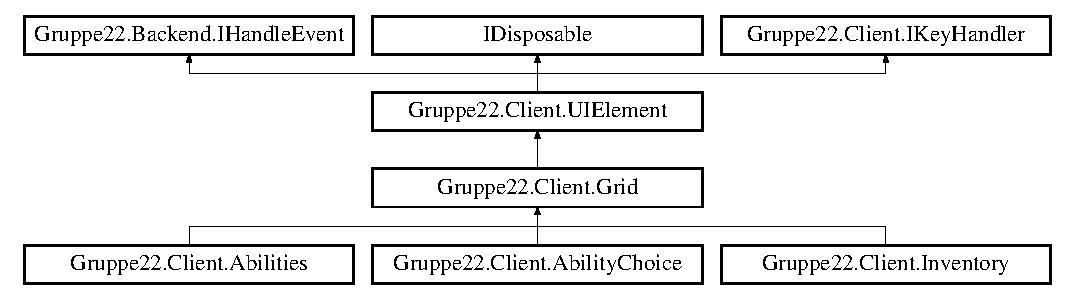
\includegraphics[height=3.589744cm]{class_gruppe22_1_1_client_1_1_grid}
\end{center}
\end{figure}
\subsection*{Öffentliche Methoden}
\begin{DoxyCompactItemize}
\item 
virtual int \hyperlink{class_gruppe22_1_1_client_1_1_grid_a7270d988d5e751a796cfd5329cbe0967}{Pos2\-Tile} (int x, int y)
\item 
void \hyperlink{class_gruppe22_1_1_client_1_1_grid_a3dc2d898edf94d5e5019b4be2128d69d}{Display\-Tool\-Tip} (int icon, int x, int y)
\begin{DoxyCompactList}\small\item\em Append a new line of text to the status box; word wrap if necessary \end{DoxyCompactList}\item 
override void \hyperlink{class_gruppe22_1_1_client_1_1_grid_a755168da3da4d1c922e81602fb01dca3}{Draw} (Game\-Time game\-Time)
\item 
override bool \hyperlink{class_gruppe22_1_1_client_1_1_grid_a73b2172889aee0a3135a62c0d1af76e9}{On\-Mouse\-Down} (int button)
\begin{DoxyCompactList}\small\item\em Called when a mouse button changes from up to down \end{DoxyCompactList}\item 
\hyperlink{class_gruppe22_1_1_client_1_1_grid_ac3ee53484aee548e11561f14f4ac62b4}{Grid} (\hyperlink{interface_gruppe22_1_1_backend_1_1_i_handle_event}{Backend.\-I\-Handle\-Event} parent, Sprite\-Batch sprite\-Batch, Content\-Manager content, Rectangle display\-Rect)
\end{DoxyCompactItemize}
\subsection*{Geschützte Attribute}
\begin{DoxyCompactItemize}
\item 
Sprite\-Font \hyperlink{class_gruppe22_1_1_client_1_1_grid_a0a38f9e91d0a62c3cf8b742535b74ad2}{\-\_\-font} = null
\item 
List$<$ \hyperlink{class_gruppe22_1_1_client_1_1_grid_element}{Grid\-Element} $>$ \hyperlink{class_gruppe22_1_1_client_1_1_grid_aa6c5b5d5d7f94edd9071c5bbd77ca24f}{\-\_\-icons}
\item 
int \hyperlink{class_gruppe22_1_1_client_1_1_grid_a933dd1b3b9af5be773bd921115c59feb}{\-\_\-rows} = 2
\item 
int \hyperlink{class_gruppe22_1_1_client_1_1_grid_a5287cb3e2ed085ccfd851f3191b2a765}{\-\_\-cols} = 3
\item 
int \hyperlink{class_gruppe22_1_1_client_1_1_grid_ad993356078eff457ab24454827b6a4e7}{\-\_\-width} = 32
\item 
int \hyperlink{class_gruppe22_1_1_client_1_1_grid_a9769cba7225642365ab38caf89cc1648}{\-\_\-height} = 32
\item 
int \hyperlink{class_gruppe22_1_1_client_1_1_grid_a009b6bc6c6f4eafc607ad05154a407ea}{\-\_\-selected} = -\/1
\item 
int \hyperlink{class_gruppe22_1_1_client_1_1_grid_a00a5a042cc916c2ccb61e71f22e2c4d8}{\-\_\-total\-Pages} = 1
\item 
int \hyperlink{class_gruppe22_1_1_client_1_1_grid_a75ea67703bd282282c9c52002912bff9}{\-\_\-page} = 0
\item 
Texture2\-D \hyperlink{class_gruppe22_1_1_client_1_1_grid_a737100c39b0ba0d03c8d0dd449785de7}{\-\_\-arrows} = null
\item 
Texture2\-D \hyperlink{class_gruppe22_1_1_client_1_1_grid_a260c6d7278902345b592e52ca0da4307}{\-\_\-background} = null
\end{DoxyCompactItemize}
\subsection*{Propertys}
\begin{DoxyCompactItemize}
\item 
int \hyperlink{class_gruppe22_1_1_client_1_1_grid_a711e8cb9cca1be9c8f3aff7c9ddbc450}{width}\hspace{0.3cm}{\ttfamily  \mbox{[}get, set\mbox{]}}
\item 
int \hyperlink{class_gruppe22_1_1_client_1_1_grid_ae1646e8080a96020555b515e1935e5b1}{height}\hspace{0.3cm}{\ttfamily  \mbox{[}get, set\mbox{]}}
\item 
int \hyperlink{class_gruppe22_1_1_client_1_1_grid_a3b4a827491fee188ce82f02746c39faf}{rows}\hspace{0.3cm}{\ttfamily  \mbox{[}get, set\mbox{]}}
\item 
int \hyperlink{class_gruppe22_1_1_client_1_1_grid_a52da03d0cf902fd7c224b17fc95b82dd}{cols}\hspace{0.3cm}{\ttfamily  \mbox{[}get, set\mbox{]}}
\end{DoxyCompactItemize}


\subsection{Ausführliche Beschreibung}




\subsection{Beschreibung der Konstruktoren und Destruktoren}
\hypertarget{class_gruppe22_1_1_client_1_1_grid_ac3ee53484aee548e11561f14f4ac62b4}{\index{Gruppe22\-::\-Client\-::\-Grid@{Gruppe22\-::\-Client\-::\-Grid}!Grid@{Grid}}
\index{Grid@{Grid}!Gruppe22::Client::Grid@{Gruppe22\-::\-Client\-::\-Grid}}
\subsubsection[{Grid}]{\setlength{\rightskip}{0pt plus 5cm}Gruppe22.\-Client.\-Grid.\-Grid (
\begin{DoxyParamCaption}
\item[{{\bf Backend.\-I\-Handle\-Event}}]{parent, }
\item[{Sprite\-Batch}]{sprite\-Batch, }
\item[{Content\-Manager}]{content, }
\item[{Rectangle}]{display\-Rect}
\end{DoxyParamCaption}
)}}\label{class_gruppe22_1_1_client_1_1_grid_ac3ee53484aee548e11561f14f4ac62b4}





\begin{DoxyParams}{Parameter}
{\em parent} & \\
\hline
{\em sprite\-Batch} & \\
\hline
{\em content} & \\
\hline
{\em display\-Rect} & \\
\hline
\end{DoxyParams}


\subsection{Dokumentation der Elementfunktionen}
\hypertarget{class_gruppe22_1_1_client_1_1_grid_a3dc2d898edf94d5e5019b4be2128d69d}{\index{Gruppe22\-::\-Client\-::\-Grid@{Gruppe22\-::\-Client\-::\-Grid}!Display\-Tool\-Tip@{Display\-Tool\-Tip}}
\index{Display\-Tool\-Tip@{Display\-Tool\-Tip}!Gruppe22::Client::Grid@{Gruppe22\-::\-Client\-::\-Grid}}
\subsubsection[{Display\-Tool\-Tip}]{\setlength{\rightskip}{0pt plus 5cm}void Gruppe22.\-Client.\-Grid.\-Display\-Tool\-Tip (
\begin{DoxyParamCaption}
\item[{int}]{icon, }
\item[{int}]{x, }
\item[{int}]{y}
\end{DoxyParamCaption}
)}}\label{class_gruppe22_1_1_client_1_1_grid_a3dc2d898edf94d5e5019b4be2128d69d}


Append a new line of text to the status box; word wrap if necessary 


\begin{DoxyParams}{Parameter}
{\em text} & \\
\hline
\end{DoxyParams}
\hypertarget{class_gruppe22_1_1_client_1_1_grid_a755168da3da4d1c922e81602fb01dca3}{\index{Gruppe22\-::\-Client\-::\-Grid@{Gruppe22\-::\-Client\-::\-Grid}!Draw@{Draw}}
\index{Draw@{Draw}!Gruppe22::Client::Grid@{Gruppe22\-::\-Client\-::\-Grid}}
\subsubsection[{Draw}]{\setlength{\rightskip}{0pt plus 5cm}override void Gruppe22.\-Client.\-Grid.\-Draw (
\begin{DoxyParamCaption}
\item[{Game\-Time}]{game\-Time}
\end{DoxyParamCaption}
)\hspace{0.3cm}{\ttfamily [virtual]}}}\label{class_gruppe22_1_1_client_1_1_grid_a755168da3da4d1c922e81602fb01dca3}





\begin{DoxyParams}{Parameter}
{\em game\-Time} & \\
\hline
\end{DoxyParams}


Erneute Implementation von \hyperlink{class_gruppe22_1_1_client_1_1_u_i_element_ae68afcbd1db3540052d6b399022e56e7}{Gruppe22.\-Client.\-U\-I\-Element}.

\hypertarget{class_gruppe22_1_1_client_1_1_grid_a73b2172889aee0a3135a62c0d1af76e9}{\index{Gruppe22\-::\-Client\-::\-Grid@{Gruppe22\-::\-Client\-::\-Grid}!On\-Mouse\-Down@{On\-Mouse\-Down}}
\index{On\-Mouse\-Down@{On\-Mouse\-Down}!Gruppe22::Client::Grid@{Gruppe22\-::\-Client\-::\-Grid}}
\subsubsection[{On\-Mouse\-Down}]{\setlength{\rightskip}{0pt plus 5cm}override bool Gruppe22.\-Client.\-Grid.\-On\-Mouse\-Down (
\begin{DoxyParamCaption}
\item[{int}]{button}
\end{DoxyParamCaption}
)\hspace{0.3cm}{\ttfamily [virtual]}}}\label{class_gruppe22_1_1_client_1_1_grid_a73b2172889aee0a3135a62c0d1af76e9}


Called when a mouse button changes from up to down 


\begin{DoxyParams}{Parameter}
{\em button} & Left \hyperlink{class_gruppe22_1_1_client_1_1_button}{Button}=1, Middle \hyperlink{class_gruppe22_1_1_client_1_1_button}{Button}=2, Right \hyperlink{class_gruppe22_1_1_client_1_1_button}{Button}=3\\
\hline
\end{DoxyParams}


Erneute Implementation von \hyperlink{class_gruppe22_1_1_client_1_1_u_i_element_a0530df2286336160b8b39c74ba380a44}{Gruppe22.\-Client.\-U\-I\-Element}.



Erneute Implementation in \hyperlink{class_gruppe22_1_1_client_1_1_inventory_a591cf287beb11b3d2f330d8f6b812e4e}{Gruppe22.\-Client.\-Inventory}.

\hypertarget{class_gruppe22_1_1_client_1_1_grid_a7270d988d5e751a796cfd5329cbe0967}{\index{Gruppe22\-::\-Client\-::\-Grid@{Gruppe22\-::\-Client\-::\-Grid}!Pos2\-Tile@{Pos2\-Tile}}
\index{Pos2\-Tile@{Pos2\-Tile}!Gruppe22::Client::Grid@{Gruppe22\-::\-Client\-::\-Grid}}
\subsubsection[{Pos2\-Tile}]{\setlength{\rightskip}{0pt plus 5cm}virtual int Gruppe22.\-Client.\-Grid.\-Pos2\-Tile (
\begin{DoxyParamCaption}
\item[{int}]{x, }
\item[{int}]{y}
\end{DoxyParamCaption}
)\hspace{0.3cm}{\ttfamily [virtual]}}}\label{class_gruppe22_1_1_client_1_1_grid_a7270d988d5e751a796cfd5329cbe0967}


Erneute Implementation in \hyperlink{class_gruppe22_1_1_client_1_1_ability_choice_a8a27d3ed23f7d873aff9a73e70775c87}{Gruppe22.\-Client.\-Ability\-Choice} und \hyperlink{class_gruppe22_1_1_client_1_1_abilities_a736694886772621f4ef219ad8ae83aa5}{Gruppe22.\-Client.\-Abilities}.



\subsection{Dokumentation der Datenelemente}
\hypertarget{class_gruppe22_1_1_client_1_1_grid_a737100c39b0ba0d03c8d0dd449785de7}{\index{Gruppe22\-::\-Client\-::\-Grid@{Gruppe22\-::\-Client\-::\-Grid}!\-\_\-arrows@{\-\_\-arrows}}
\index{\-\_\-arrows@{\-\_\-arrows}!Gruppe22::Client::Grid@{Gruppe22\-::\-Client\-::\-Grid}}
\subsubsection[{\-\_\-arrows}]{\setlength{\rightskip}{0pt plus 5cm}Texture2\-D Gruppe22.\-Client.\-Grid.\-\_\-arrows = null\hspace{0.3cm}{\ttfamily [protected]}}}\label{class_gruppe22_1_1_client_1_1_grid_a737100c39b0ba0d03c8d0dd449785de7}
\hypertarget{class_gruppe22_1_1_client_1_1_grid_a260c6d7278902345b592e52ca0da4307}{\index{Gruppe22\-::\-Client\-::\-Grid@{Gruppe22\-::\-Client\-::\-Grid}!\-\_\-background@{\-\_\-background}}
\index{\-\_\-background@{\-\_\-background}!Gruppe22::Client::Grid@{Gruppe22\-::\-Client\-::\-Grid}}
\subsubsection[{\-\_\-background}]{\setlength{\rightskip}{0pt plus 5cm}Texture2\-D Gruppe22.\-Client.\-Grid.\-\_\-background = null\hspace{0.3cm}{\ttfamily [protected]}}}\label{class_gruppe22_1_1_client_1_1_grid_a260c6d7278902345b592e52ca0da4307}
\hypertarget{class_gruppe22_1_1_client_1_1_grid_a5287cb3e2ed085ccfd851f3191b2a765}{\index{Gruppe22\-::\-Client\-::\-Grid@{Gruppe22\-::\-Client\-::\-Grid}!\-\_\-cols@{\-\_\-cols}}
\index{\-\_\-cols@{\-\_\-cols}!Gruppe22::Client::Grid@{Gruppe22\-::\-Client\-::\-Grid}}
\subsubsection[{\-\_\-cols}]{\setlength{\rightskip}{0pt plus 5cm}int Gruppe22.\-Client.\-Grid.\-\_\-cols = 3\hspace{0.3cm}{\ttfamily [protected]}}}\label{class_gruppe22_1_1_client_1_1_grid_a5287cb3e2ed085ccfd851f3191b2a765}




\hypertarget{class_gruppe22_1_1_client_1_1_grid_a0a38f9e91d0a62c3cf8b742535b74ad2}{\index{Gruppe22\-::\-Client\-::\-Grid@{Gruppe22\-::\-Client\-::\-Grid}!\-\_\-font@{\-\_\-font}}
\index{\-\_\-font@{\-\_\-font}!Gruppe22::Client::Grid@{Gruppe22\-::\-Client\-::\-Grid}}
\subsubsection[{\-\_\-font}]{\setlength{\rightskip}{0pt plus 5cm}Sprite\-Font Gruppe22.\-Client.\-Grid.\-\_\-font = null\hspace{0.3cm}{\ttfamily [protected]}}}\label{class_gruppe22_1_1_client_1_1_grid_a0a38f9e91d0a62c3cf8b742535b74ad2}
\hypertarget{class_gruppe22_1_1_client_1_1_grid_a9769cba7225642365ab38caf89cc1648}{\index{Gruppe22\-::\-Client\-::\-Grid@{Gruppe22\-::\-Client\-::\-Grid}!\-\_\-height@{\-\_\-height}}
\index{\-\_\-height@{\-\_\-height}!Gruppe22::Client::Grid@{Gruppe22\-::\-Client\-::\-Grid}}
\subsubsection[{\-\_\-height}]{\setlength{\rightskip}{0pt plus 5cm}int Gruppe22.\-Client.\-Grid.\-\_\-height = 32\hspace{0.3cm}{\ttfamily [protected]}}}\label{class_gruppe22_1_1_client_1_1_grid_a9769cba7225642365ab38caf89cc1648}




\hypertarget{class_gruppe22_1_1_client_1_1_grid_aa6c5b5d5d7f94edd9071c5bbd77ca24f}{\index{Gruppe22\-::\-Client\-::\-Grid@{Gruppe22\-::\-Client\-::\-Grid}!\-\_\-icons@{\-\_\-icons}}
\index{\-\_\-icons@{\-\_\-icons}!Gruppe22::Client::Grid@{Gruppe22\-::\-Client\-::\-Grid}}
\subsubsection[{\-\_\-icons}]{\setlength{\rightskip}{0pt plus 5cm}List$<${\bf Grid\-Element}$>$ Gruppe22.\-Client.\-Grid.\-\_\-icons\hspace{0.3cm}{\ttfamily [protected]}}}\label{class_gruppe22_1_1_client_1_1_grid_aa6c5b5d5d7f94edd9071c5bbd77ca24f}




\hypertarget{class_gruppe22_1_1_client_1_1_grid_a75ea67703bd282282c9c52002912bff9}{\index{Gruppe22\-::\-Client\-::\-Grid@{Gruppe22\-::\-Client\-::\-Grid}!\-\_\-page@{\-\_\-page}}
\index{\-\_\-page@{\-\_\-page}!Gruppe22::Client::Grid@{Gruppe22\-::\-Client\-::\-Grid}}
\subsubsection[{\-\_\-page}]{\setlength{\rightskip}{0pt plus 5cm}int Gruppe22.\-Client.\-Grid.\-\_\-page = 0\hspace{0.3cm}{\ttfamily [protected]}}}\label{class_gruppe22_1_1_client_1_1_grid_a75ea67703bd282282c9c52002912bff9}




\hypertarget{class_gruppe22_1_1_client_1_1_grid_a933dd1b3b9af5be773bd921115c59feb}{\index{Gruppe22\-::\-Client\-::\-Grid@{Gruppe22\-::\-Client\-::\-Grid}!\-\_\-rows@{\-\_\-rows}}
\index{\-\_\-rows@{\-\_\-rows}!Gruppe22::Client::Grid@{Gruppe22\-::\-Client\-::\-Grid}}
\subsubsection[{\-\_\-rows}]{\setlength{\rightskip}{0pt plus 5cm}int Gruppe22.\-Client.\-Grid.\-\_\-rows = 2\hspace{0.3cm}{\ttfamily [protected]}}}\label{class_gruppe22_1_1_client_1_1_grid_a933dd1b3b9af5be773bd921115c59feb}




\hypertarget{class_gruppe22_1_1_client_1_1_grid_a009b6bc6c6f4eafc607ad05154a407ea}{\index{Gruppe22\-::\-Client\-::\-Grid@{Gruppe22\-::\-Client\-::\-Grid}!\-\_\-selected@{\-\_\-selected}}
\index{\-\_\-selected@{\-\_\-selected}!Gruppe22::Client::Grid@{Gruppe22\-::\-Client\-::\-Grid}}
\subsubsection[{\-\_\-selected}]{\setlength{\rightskip}{0pt plus 5cm}int Gruppe22.\-Client.\-Grid.\-\_\-selected = -\/1\hspace{0.3cm}{\ttfamily [protected]}}}\label{class_gruppe22_1_1_client_1_1_grid_a009b6bc6c6f4eafc607ad05154a407ea}




\hypertarget{class_gruppe22_1_1_client_1_1_grid_a00a5a042cc916c2ccb61e71f22e2c4d8}{\index{Gruppe22\-::\-Client\-::\-Grid@{Gruppe22\-::\-Client\-::\-Grid}!\-\_\-total\-Pages@{\-\_\-total\-Pages}}
\index{\-\_\-total\-Pages@{\-\_\-total\-Pages}!Gruppe22::Client::Grid@{Gruppe22\-::\-Client\-::\-Grid}}
\subsubsection[{\-\_\-total\-Pages}]{\setlength{\rightskip}{0pt plus 5cm}int Gruppe22.\-Client.\-Grid.\-\_\-total\-Pages = 1\hspace{0.3cm}{\ttfamily [protected]}}}\label{class_gruppe22_1_1_client_1_1_grid_a00a5a042cc916c2ccb61e71f22e2c4d8}




\hypertarget{class_gruppe22_1_1_client_1_1_grid_ad993356078eff457ab24454827b6a4e7}{\index{Gruppe22\-::\-Client\-::\-Grid@{Gruppe22\-::\-Client\-::\-Grid}!\-\_\-width@{\-\_\-width}}
\index{\-\_\-width@{\-\_\-width}!Gruppe22::Client::Grid@{Gruppe22\-::\-Client\-::\-Grid}}
\subsubsection[{\-\_\-width}]{\setlength{\rightskip}{0pt plus 5cm}int Gruppe22.\-Client.\-Grid.\-\_\-width = 32\hspace{0.3cm}{\ttfamily [protected]}}}\label{class_gruppe22_1_1_client_1_1_grid_ad993356078eff457ab24454827b6a4e7}






\subsection{Dokumentation der Propertys}
\hypertarget{class_gruppe22_1_1_client_1_1_grid_a52da03d0cf902fd7c224b17fc95b82dd}{\index{Gruppe22\-::\-Client\-::\-Grid@{Gruppe22\-::\-Client\-::\-Grid}!cols@{cols}}
\index{cols@{cols}!Gruppe22::Client::Grid@{Gruppe22\-::\-Client\-::\-Grid}}
\subsubsection[{cols}]{\setlength{\rightskip}{0pt plus 5cm}int Gruppe22.\-Client.\-Grid.\-cols\hspace{0.3cm}{\ttfamily [get]}, {\ttfamily [set]}}}\label{class_gruppe22_1_1_client_1_1_grid_a52da03d0cf902fd7c224b17fc95b82dd}




\hypertarget{class_gruppe22_1_1_client_1_1_grid_ae1646e8080a96020555b515e1935e5b1}{\index{Gruppe22\-::\-Client\-::\-Grid@{Gruppe22\-::\-Client\-::\-Grid}!height@{height}}
\index{height@{height}!Gruppe22::Client::Grid@{Gruppe22\-::\-Client\-::\-Grid}}
\subsubsection[{height}]{\setlength{\rightskip}{0pt plus 5cm}int Gruppe22.\-Client.\-Grid.\-height\hspace{0.3cm}{\ttfamily [get]}, {\ttfamily [set]}}}\label{class_gruppe22_1_1_client_1_1_grid_ae1646e8080a96020555b515e1935e5b1}




\hypertarget{class_gruppe22_1_1_client_1_1_grid_a3b4a827491fee188ce82f02746c39faf}{\index{Gruppe22\-::\-Client\-::\-Grid@{Gruppe22\-::\-Client\-::\-Grid}!rows@{rows}}
\index{rows@{rows}!Gruppe22::Client::Grid@{Gruppe22\-::\-Client\-::\-Grid}}
\subsubsection[{rows}]{\setlength{\rightskip}{0pt plus 5cm}int Gruppe22.\-Client.\-Grid.\-rows\hspace{0.3cm}{\ttfamily [get]}, {\ttfamily [set]}}}\label{class_gruppe22_1_1_client_1_1_grid_a3b4a827491fee188ce82f02746c39faf}




\hypertarget{class_gruppe22_1_1_client_1_1_grid_a711e8cb9cca1be9c8f3aff7c9ddbc450}{\index{Gruppe22\-::\-Client\-::\-Grid@{Gruppe22\-::\-Client\-::\-Grid}!width@{width}}
\index{width@{width}!Gruppe22::Client::Grid@{Gruppe22\-::\-Client\-::\-Grid}}
\subsubsection[{width}]{\setlength{\rightskip}{0pt plus 5cm}int Gruppe22.\-Client.\-Grid.\-width\hspace{0.3cm}{\ttfamily [get]}, {\ttfamily [set]}}}\label{class_gruppe22_1_1_client_1_1_grid_a711e8cb9cca1be9c8f3aff7c9ddbc450}






Die Dokumentation für diese Klasse wurde erzeugt aufgrund der Datei\-:\begin{DoxyCompactItemize}
\item 
C\-:/\-Users/beursken/\-Documents/\-Git\-Hub/gruppe22/\-Gruppe22/\-Gruppe22/\-Client/\-U\-I/\hyperlink{_grid_8cs}{Grid.\-cs}\end{DoxyCompactItemize}

\hypertarget{class_gruppe22_1_1_client_1_1_grid_element}{\section{Gruppe22.\-Client.\-Grid\-Element Klassenreferenz}
\label{class_gruppe22_1_1_client_1_1_grid_element}\index{Gruppe22.\-Client.\-Grid\-Element@{Gruppe22.\-Client.\-Grid\-Element}}
}
\subsection*{Öffentliche Methoden}
\begin{DoxyCompactItemize}
\item 
\hyperlink{class_gruppe22_1_1_client_1_1_grid_element_a61548e525729e284b79b5c62242a21e5}{Grid\-Element} (int \hyperlink{class_gruppe22_1_1_client_1_1_grid_element_ade695078dc93f47e1f5891408d65d7a7}{id}, string \hyperlink{class_gruppe22_1_1_client_1_1_grid_element_ae5630d8dff48a5516d96af9ce6da566f}{tooltip}, \hyperlink{class_gruppe22_1_1_backend_1_1_image_data}{Backend.\-Image\-Data} \hyperlink{class_gruppe22_1_1_client_1_1_grid_element_a2a648989f64d0d4d897496958b01b7b0}{icon}, Content\-Manager content, bool Checked, bool \hyperlink{class_gruppe22_1_1_client_1_1_grid_element_a1f939562cf4dca6a69de78dd3a44a1fe}{enabled}=true, int \hyperlink{class_gruppe22_1_1_client_1_1_grid_element_a3d2ee9e08f1d3fbbf3b3e8b09d7fd5c3}{flash}=0)
\item 
\hyperlink{class_gruppe22_1_1_client_1_1_grid_element_a253fdf7cf4779c99006b4a2c3422ecc7}{Grid\-Element} (int \hyperlink{class_gruppe22_1_1_client_1_1_grid_element_ade695078dc93f47e1f5891408d65d7a7}{id}, string \hyperlink{class_gruppe22_1_1_client_1_1_grid_element_ae5630d8dff48a5516d96af9ce6da566f}{tooltip}, \hyperlink{class_gruppe22_1_1_client_1_1_visible_object}{Visible\-Object} \hyperlink{class_gruppe22_1_1_client_1_1_grid_element_a2a648989f64d0d4d897496958b01b7b0}{icon}, bool Checked, bool \hyperlink{class_gruppe22_1_1_client_1_1_grid_element_a1f939562cf4dca6a69de78dd3a44a1fe}{enabled}=true, int \hyperlink{class_gruppe22_1_1_client_1_1_grid_element_a3d2ee9e08f1d3fbbf3b3e8b09d7fd5c3}{flash}=0)
\end{DoxyCompactItemize}
\subsection*{Propertys}
\begin{DoxyCompactItemize}
\item 
\hyperlink{class_gruppe22_1_1_client_1_1_visible_object}{Visible\-Object} \hyperlink{class_gruppe22_1_1_client_1_1_grid_element_a2a648989f64d0d4d897496958b01b7b0}{icon}\hspace{0.3cm}{\ttfamily  \mbox{[}get, set\mbox{]}}
\item 
string \hyperlink{class_gruppe22_1_1_client_1_1_grid_element_ae5630d8dff48a5516d96af9ce6da566f}{tooltip}\hspace{0.3cm}{\ttfamily  \mbox{[}get, set\mbox{]}}
\item 
int \hyperlink{class_gruppe22_1_1_client_1_1_grid_element_ade695078dc93f47e1f5891408d65d7a7}{id}\hspace{0.3cm}{\ttfamily  \mbox{[}get, set\mbox{]}}
\item 
bool \hyperlink{class_gruppe22_1_1_client_1_1_grid_element_a7d190359527abea90226cc24a49e7a75}{check}\hspace{0.3cm}{\ttfamily  \mbox{[}get, set\mbox{]}}
\item 
int \hyperlink{class_gruppe22_1_1_client_1_1_grid_element_a3d2ee9e08f1d3fbbf3b3e8b09d7fd5c3}{flash}\hspace{0.3cm}{\ttfamily  \mbox{[}get, set\mbox{]}}
\item 
bool \hyperlink{class_gruppe22_1_1_client_1_1_grid_element_a1f939562cf4dca6a69de78dd3a44a1fe}{enabled}\hspace{0.3cm}{\ttfamily  \mbox{[}get, set\mbox{]}}
\end{DoxyCompactItemize}


\subsection{Beschreibung der Konstruktoren und Destruktoren}
\hypertarget{class_gruppe22_1_1_client_1_1_grid_element_a61548e525729e284b79b5c62242a21e5}{\index{Gruppe22\-::\-Client\-::\-Grid\-Element@{Gruppe22\-::\-Client\-::\-Grid\-Element}!Grid\-Element@{Grid\-Element}}
\index{Grid\-Element@{Grid\-Element}!Gruppe22::Client::GridElement@{Gruppe22\-::\-Client\-::\-Grid\-Element}}
\subsubsection[{Grid\-Element}]{\setlength{\rightskip}{0pt plus 5cm}Gruppe22.\-Client.\-Grid\-Element.\-Grid\-Element (
\begin{DoxyParamCaption}
\item[{int}]{id, }
\item[{string}]{tooltip, }
\item[{{\bf Backend.\-Image\-Data}}]{icon, }
\item[{Content\-Manager}]{content, }
\item[{bool}]{Checked, }
\item[{bool}]{enabled = {\ttfamily true}, }
\item[{int}]{flash = {\ttfamily 0}}
\end{DoxyParamCaption}
)}}\label{class_gruppe22_1_1_client_1_1_grid_element_a61548e525729e284b79b5c62242a21e5}
\hypertarget{class_gruppe22_1_1_client_1_1_grid_element_a253fdf7cf4779c99006b4a2c3422ecc7}{\index{Gruppe22\-::\-Client\-::\-Grid\-Element@{Gruppe22\-::\-Client\-::\-Grid\-Element}!Grid\-Element@{Grid\-Element}}
\index{Grid\-Element@{Grid\-Element}!Gruppe22::Client::GridElement@{Gruppe22\-::\-Client\-::\-Grid\-Element}}
\subsubsection[{Grid\-Element}]{\setlength{\rightskip}{0pt plus 5cm}Gruppe22.\-Client.\-Grid\-Element.\-Grid\-Element (
\begin{DoxyParamCaption}
\item[{int}]{id, }
\item[{string}]{tooltip, }
\item[{{\bf Visible\-Object}}]{icon, }
\item[{bool}]{Checked, }
\item[{bool}]{enabled = {\ttfamily true}, }
\item[{int}]{flash = {\ttfamily 0}}
\end{DoxyParamCaption}
)}}\label{class_gruppe22_1_1_client_1_1_grid_element_a253fdf7cf4779c99006b4a2c3422ecc7}


\subsection{Dokumentation der Propertys}
\hypertarget{class_gruppe22_1_1_client_1_1_grid_element_a7d190359527abea90226cc24a49e7a75}{\index{Gruppe22\-::\-Client\-::\-Grid\-Element@{Gruppe22\-::\-Client\-::\-Grid\-Element}!check@{check}}
\index{check@{check}!Gruppe22::Client::GridElement@{Gruppe22\-::\-Client\-::\-Grid\-Element}}
\subsubsection[{check}]{\setlength{\rightskip}{0pt plus 5cm}bool Gruppe22.\-Client.\-Grid\-Element.\-check\hspace{0.3cm}{\ttfamily [get]}, {\ttfamily [set]}}}\label{class_gruppe22_1_1_client_1_1_grid_element_a7d190359527abea90226cc24a49e7a75}
\hypertarget{class_gruppe22_1_1_client_1_1_grid_element_a1f939562cf4dca6a69de78dd3a44a1fe}{\index{Gruppe22\-::\-Client\-::\-Grid\-Element@{Gruppe22\-::\-Client\-::\-Grid\-Element}!enabled@{enabled}}
\index{enabled@{enabled}!Gruppe22::Client::GridElement@{Gruppe22\-::\-Client\-::\-Grid\-Element}}
\subsubsection[{enabled}]{\setlength{\rightskip}{0pt plus 5cm}bool Gruppe22.\-Client.\-Grid\-Element.\-enabled\hspace{0.3cm}{\ttfamily [get]}, {\ttfamily [set]}}}\label{class_gruppe22_1_1_client_1_1_grid_element_a1f939562cf4dca6a69de78dd3a44a1fe}
\hypertarget{class_gruppe22_1_1_client_1_1_grid_element_a3d2ee9e08f1d3fbbf3b3e8b09d7fd5c3}{\index{Gruppe22\-::\-Client\-::\-Grid\-Element@{Gruppe22\-::\-Client\-::\-Grid\-Element}!flash@{flash}}
\index{flash@{flash}!Gruppe22::Client::GridElement@{Gruppe22\-::\-Client\-::\-Grid\-Element}}
\subsubsection[{flash}]{\setlength{\rightskip}{0pt plus 5cm}int Gruppe22.\-Client.\-Grid\-Element.\-flash\hspace{0.3cm}{\ttfamily [get]}, {\ttfamily [set]}}}\label{class_gruppe22_1_1_client_1_1_grid_element_a3d2ee9e08f1d3fbbf3b3e8b09d7fd5c3}
\hypertarget{class_gruppe22_1_1_client_1_1_grid_element_a2a648989f64d0d4d897496958b01b7b0}{\index{Gruppe22\-::\-Client\-::\-Grid\-Element@{Gruppe22\-::\-Client\-::\-Grid\-Element}!icon@{icon}}
\index{icon@{icon}!Gruppe22::Client::GridElement@{Gruppe22\-::\-Client\-::\-Grid\-Element}}
\subsubsection[{icon}]{\setlength{\rightskip}{0pt plus 5cm}{\bf Visible\-Object} Gruppe22.\-Client.\-Grid\-Element.\-icon\hspace{0.3cm}{\ttfamily [get]}, {\ttfamily [set]}}}\label{class_gruppe22_1_1_client_1_1_grid_element_a2a648989f64d0d4d897496958b01b7b0}
\hypertarget{class_gruppe22_1_1_client_1_1_grid_element_ade695078dc93f47e1f5891408d65d7a7}{\index{Gruppe22\-::\-Client\-::\-Grid\-Element@{Gruppe22\-::\-Client\-::\-Grid\-Element}!id@{id}}
\index{id@{id}!Gruppe22::Client::GridElement@{Gruppe22\-::\-Client\-::\-Grid\-Element}}
\subsubsection[{id}]{\setlength{\rightskip}{0pt plus 5cm}int Gruppe22.\-Client.\-Grid\-Element.\-id\hspace{0.3cm}{\ttfamily [get]}, {\ttfamily [set]}}}\label{class_gruppe22_1_1_client_1_1_grid_element_ade695078dc93f47e1f5891408d65d7a7}
\hypertarget{class_gruppe22_1_1_client_1_1_grid_element_ae5630d8dff48a5516d96af9ce6da566f}{\index{Gruppe22\-::\-Client\-::\-Grid\-Element@{Gruppe22\-::\-Client\-::\-Grid\-Element}!tooltip@{tooltip}}
\index{tooltip@{tooltip}!Gruppe22::Client::GridElement@{Gruppe22\-::\-Client\-::\-Grid\-Element}}
\subsubsection[{tooltip}]{\setlength{\rightskip}{0pt plus 5cm}string Gruppe22.\-Client.\-Grid\-Element.\-tooltip\hspace{0.3cm}{\ttfamily [get]}, {\ttfamily [set]}}}\label{class_gruppe22_1_1_client_1_1_grid_element_ae5630d8dff48a5516d96af9ce6da566f}


Die Dokumentation für diese Klasse wurde erzeugt aufgrund der Datei\-:\begin{DoxyCompactItemize}
\item 
C\-:/\-Users/beursken/\-Documents/\-Git\-Hub/gruppe22/\-Gruppe22/\-Gruppe22/\-Client/\-U\-I/\hyperlink{_grid_8cs}{Grid.\-cs}\end{DoxyCompactItemize}

\hypertarget{interface_gruppe22_1_1_backend_1_1_i_handle_event}{\section{Gruppe22.\-Backend.\-I\-Handle\-Event Schnittstellenreferenz}
\label{interface_gruppe22_1_1_backend_1_1_i_handle_event}\index{Gruppe22.\-Backend.\-I\-Handle\-Event@{Gruppe22.\-Backend.\-I\-Handle\-Event}}
}
Klassendiagramm für Gruppe22.\-Backend.\-I\-Handle\-Event\-:\begin{figure}[H]
\begin{center}
\leavevmode
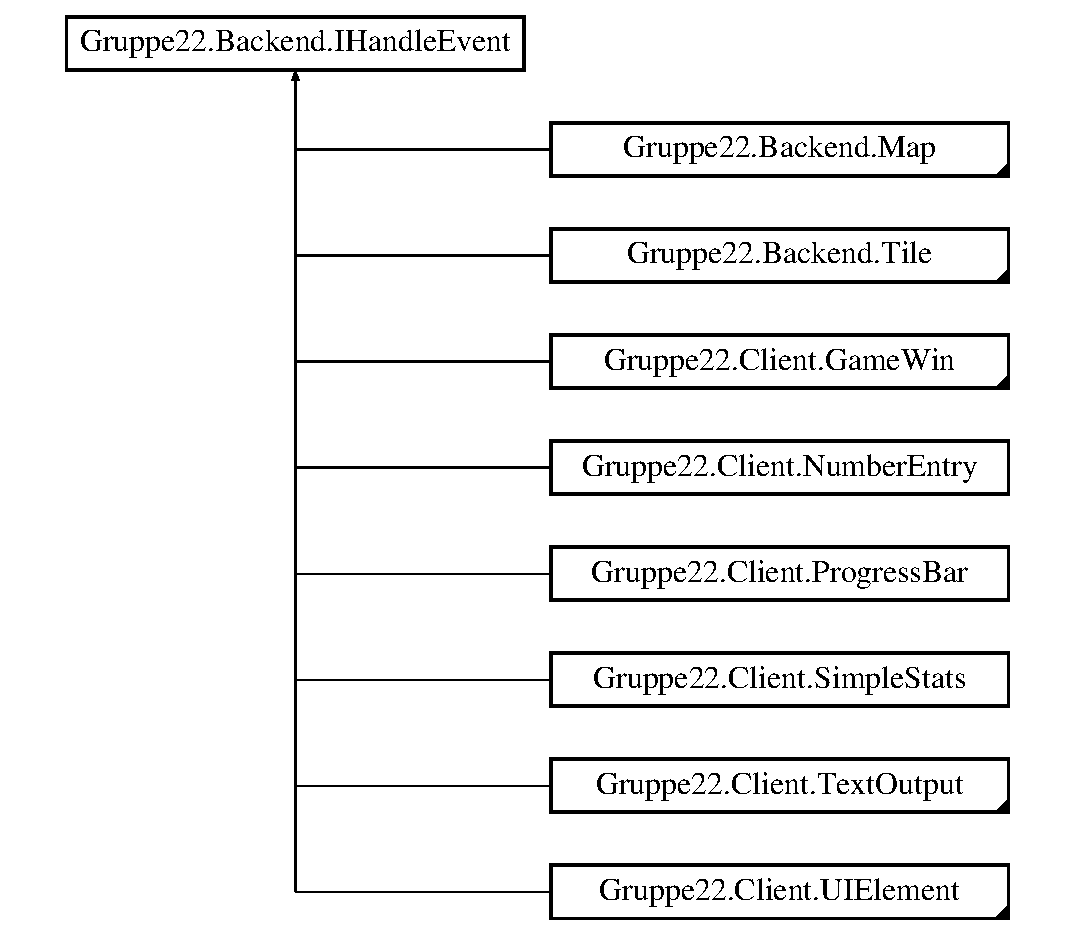
\includegraphics[height=9.000000cm]{interface_gruppe22_1_1_backend_1_1_i_handle_event}
\end{center}
\end{figure}
\subsection*{Öffentliche Methoden}
\begin{DoxyCompactItemize}
\item 
void \hyperlink{interface_gruppe22_1_1_backend_1_1_i_handle_event_a84b03cc5988da83a6303307812ea2a5e}{Handle\-Event} (bool Down\-Stream, \hyperlink{namespace_gruppe22_1_1_backend_ab56df91bb0bdafa1ea978e552209ce73}{Backend.\-Events} event\-I\-D, params object\mbox{[}$\,$\mbox{]} data)
\end{DoxyCompactItemize}


\subsection{Dokumentation der Elementfunktionen}
\hypertarget{interface_gruppe22_1_1_backend_1_1_i_handle_event_a84b03cc5988da83a6303307812ea2a5e}{\index{Gruppe22\-::\-Backend\-::\-I\-Handle\-Event@{Gruppe22\-::\-Backend\-::\-I\-Handle\-Event}!Handle\-Event@{Handle\-Event}}
\index{Handle\-Event@{Handle\-Event}!Gruppe22::Backend::IHandleEvent@{Gruppe22\-::\-Backend\-::\-I\-Handle\-Event}}
\subsubsection[{Handle\-Event}]{\setlength{\rightskip}{0pt plus 5cm}void Gruppe22.\-Backend.\-I\-Handle\-Event.\-Handle\-Event (
\begin{DoxyParamCaption}
\item[{bool}]{Down\-Stream, }
\item[{{\bf Backend.\-Events}}]{event\-I\-D, }
\item[{params object\mbox{[}$\,$\mbox{]}}]{data}
\end{DoxyParamCaption}
)}}\label{interface_gruppe22_1_1_backend_1_1_i_handle_event_a84b03cc5988da83a6303307812ea2a5e}


Die Dokumentation für diese Schnittstelle wurde erzeugt aufgrund der Datei\-:\begin{DoxyCompactItemize}
\item 
C\-:/\-Users/beursken/\-Documents/\-Git\-Hub/gruppe22/\-Gruppe22/\-Gruppe22/\-Backend/\hyperlink{_helpers_8cs}{Helpers.\-cs}\end{DoxyCompactItemize}

\hypertarget{interface_gruppe22_1_1_client_1_1_i_key_handler}{\section{Gruppe22.\-Client.\-I\-Key\-Handler Schnittstellenreferenz}
\label{interface_gruppe22_1_1_client_1_1_i_key_handler}\index{Gruppe22.\-Client.\-I\-Key\-Handler@{Gruppe22.\-Client.\-I\-Key\-Handler}}
}


An interface to emulate Windows Forms style key and mouse events  


Klassendiagramm für Gruppe22.\-Client.\-I\-Key\-Handler\-:\begin{figure}[H]
\begin{center}
\leavevmode
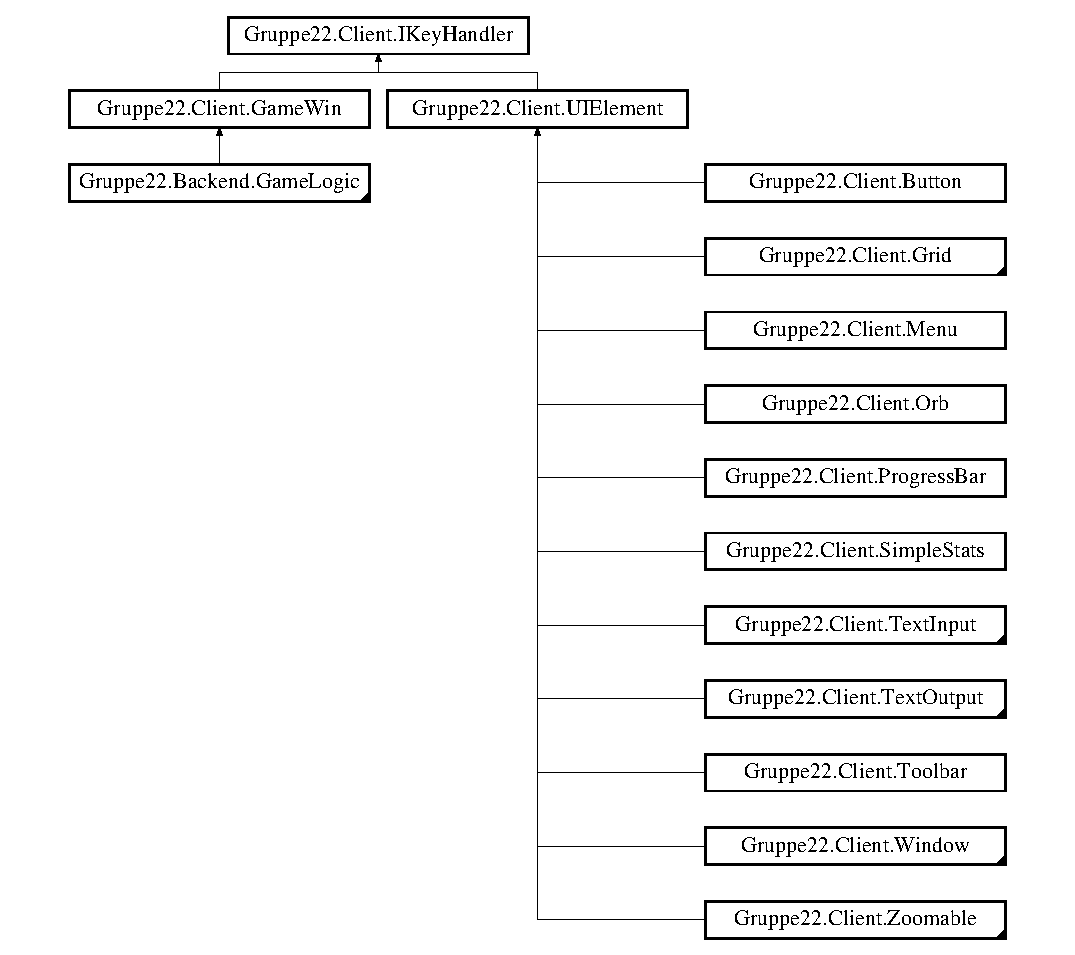
\includegraphics[height=12.000000cm]{interface_gruppe22_1_1_client_1_1_i_key_handler}
\end{center}
\end{figure}
\subsection*{Öffentliche Methoden}
\begin{DoxyCompactItemize}
\item 
bool \hyperlink{interface_gruppe22_1_1_client_1_1_i_key_handler_a3816611e429cab857650f672fda4632b}{On\-Key\-Down} (Keys k)
\begin{DoxyCompactList}\small\item\em Called whenever a key was up and is now down \end{DoxyCompactList}\item 
bool \hyperlink{interface_gruppe22_1_1_client_1_1_i_key_handler_adf473af0ebd0c8a3a22ba252ed381356}{On\-Key\-Up} (Keys k)
\begin{DoxyCompactList}\small\item\em Called whenever a key was down and is now up \end{DoxyCompactList}\item 
bool \hyperlink{interface_gruppe22_1_1_client_1_1_i_key_handler_a6e52139cdd4408abdd31e61ce1e69991}{On\-Mouse\-Down} (int button)
\begin{DoxyCompactList}\small\item\em Called when a mouse button changes from up to down \end{DoxyCompactList}\item 
bool \hyperlink{interface_gruppe22_1_1_client_1_1_i_key_handler_ad1fd9aa17fc6f8328beddd59cef28499}{On\-Mouse\-Up} (int button)
\begin{DoxyCompactList}\small\item\em Called when a mouse button changes from down to up \end{DoxyCompactList}\item 
bool \hyperlink{interface_gruppe22_1_1_client_1_1_i_key_handler_aa66a6080c4ea14b63a5578882b9f3b3e}{On\-Mouse\-Held} (int button)
\item 
bool \hyperlink{interface_gruppe22_1_1_client_1_1_i_key_handler_a4196bd333be759f8ade7996f58ca39d6}{On\-Key\-Held} (Keys k)
\end{DoxyCompactItemize}


\subsection{Ausführliche Beschreibung}
An interface to emulate Windows Forms style key and mouse events 



\subsection{Dokumentation der Elementfunktionen}
\hypertarget{interface_gruppe22_1_1_client_1_1_i_key_handler_a3816611e429cab857650f672fda4632b}{\index{Gruppe22\-::\-Client\-::\-I\-Key\-Handler@{Gruppe22\-::\-Client\-::\-I\-Key\-Handler}!On\-Key\-Down@{On\-Key\-Down}}
\index{On\-Key\-Down@{On\-Key\-Down}!Gruppe22::Client::IKeyHandler@{Gruppe22\-::\-Client\-::\-I\-Key\-Handler}}
\subsubsection[{On\-Key\-Down}]{\setlength{\rightskip}{0pt plus 5cm}bool Gruppe22.\-Client.\-I\-Key\-Handler.\-On\-Key\-Down (
\begin{DoxyParamCaption}
\item[{Keys}]{k}
\end{DoxyParamCaption}
)}}\label{interface_gruppe22_1_1_client_1_1_i_key_handler_a3816611e429cab857650f672fda4632b}


Called whenever a key was up and is now down 


\begin{DoxyParams}{Parameter}
{\em k} & The key which was pressed\\
\hline
\end{DoxyParams}


Implementiert in \hyperlink{class_gruppe22_1_1_client_1_1_game_win_aba7e900502db9021072b1c85ec2f249a}{Gruppe22.\-Client.\-Game\-Win}, \hyperlink{class_gruppe22_1_1_client_1_1_statusbox_a92512ba8bfcfeb6c417eedf5f1b3634e}{Gruppe22.\-Client.\-Statusbox}, \hyperlink{class_gruppe22_1_1_client_1_1_button_ad3b8e8bceadd5999af01485ed178446b}{Gruppe22.\-Client.\-Button}, \hyperlink{class_gruppe22_1_1_client_1_1_zoomable_a123f31a025a85e07001dab61a8102881}{Gruppe22.\-Client.\-Zoomable}, \hyperlink{class_gruppe22_1_1_client_1_1_window_ac71cd9635bec479f506ae2e7096b6617}{Gruppe22.\-Client.\-Window} und \hyperlink{class_gruppe22_1_1_client_1_1_u_i_element_a0f9957f48ecb697ff5ae1ac3f0873064}{Gruppe22.\-Client.\-U\-I\-Element}.

\hypertarget{interface_gruppe22_1_1_client_1_1_i_key_handler_a4196bd333be759f8ade7996f58ca39d6}{\index{Gruppe22\-::\-Client\-::\-I\-Key\-Handler@{Gruppe22\-::\-Client\-::\-I\-Key\-Handler}!On\-Key\-Held@{On\-Key\-Held}}
\index{On\-Key\-Held@{On\-Key\-Held}!Gruppe22::Client::IKeyHandler@{Gruppe22\-::\-Client\-::\-I\-Key\-Handler}}
\subsubsection[{On\-Key\-Held}]{\setlength{\rightskip}{0pt plus 5cm}bool Gruppe22.\-Client.\-I\-Key\-Handler.\-On\-Key\-Held (
\begin{DoxyParamCaption}
\item[{Keys}]{k}
\end{DoxyParamCaption}
)}}\label{interface_gruppe22_1_1_client_1_1_i_key_handler_a4196bd333be759f8ade7996f58ca39d6}


Implementiert in \hyperlink{class_gruppe22_1_1_client_1_1_game_win_a9a74789da3ac1c1fa9ac35541db76c6d}{Gruppe22.\-Client.\-Game\-Win}, \hyperlink{class_gruppe22_1_1_client_1_1_u_i_element_a00a8a507f4701226bd2406ae501750d6}{Gruppe22.\-Client.\-U\-I\-Element} und \hyperlink{class_gruppe22_1_1_client_1_1_zoomable_ac2965c52d19ec510714c511583ec4b36}{Gruppe22.\-Client.\-Zoomable}.

\hypertarget{interface_gruppe22_1_1_client_1_1_i_key_handler_adf473af0ebd0c8a3a22ba252ed381356}{\index{Gruppe22\-::\-Client\-::\-I\-Key\-Handler@{Gruppe22\-::\-Client\-::\-I\-Key\-Handler}!On\-Key\-Up@{On\-Key\-Up}}
\index{On\-Key\-Up@{On\-Key\-Up}!Gruppe22::Client::IKeyHandler@{Gruppe22\-::\-Client\-::\-I\-Key\-Handler}}
\subsubsection[{On\-Key\-Up}]{\setlength{\rightskip}{0pt plus 5cm}bool Gruppe22.\-Client.\-I\-Key\-Handler.\-On\-Key\-Up (
\begin{DoxyParamCaption}
\item[{Keys}]{k}
\end{DoxyParamCaption}
)}}\label{interface_gruppe22_1_1_client_1_1_i_key_handler_adf473af0ebd0c8a3a22ba252ed381356}


Called whenever a key was down and is now up 


\begin{DoxyParams}{Parameter}
{\em k} & The key which was pressed\\
\hline
\end{DoxyParams}


Implementiert in \hyperlink{class_gruppe22_1_1_client_1_1_game_win_a9bab3243c9a2b2aaf135f0da6eac7ea3}{Gruppe22.\-Client.\-Game\-Win} und \hyperlink{class_gruppe22_1_1_client_1_1_u_i_element_a555436883e05d5c2df8aff0d1b5230ab}{Gruppe22.\-Client.\-U\-I\-Element}.

\hypertarget{interface_gruppe22_1_1_client_1_1_i_key_handler_a6e52139cdd4408abdd31e61ce1e69991}{\index{Gruppe22\-::\-Client\-::\-I\-Key\-Handler@{Gruppe22\-::\-Client\-::\-I\-Key\-Handler}!On\-Mouse\-Down@{On\-Mouse\-Down}}
\index{On\-Mouse\-Down@{On\-Mouse\-Down}!Gruppe22::Client::IKeyHandler@{Gruppe22\-::\-Client\-::\-I\-Key\-Handler}}
\subsubsection[{On\-Mouse\-Down}]{\setlength{\rightskip}{0pt plus 5cm}bool Gruppe22.\-Client.\-I\-Key\-Handler.\-On\-Mouse\-Down (
\begin{DoxyParamCaption}
\item[{int}]{button}
\end{DoxyParamCaption}
)}}\label{interface_gruppe22_1_1_client_1_1_i_key_handler_a6e52139cdd4408abdd31e61ce1e69991}


Called when a mouse button changes from up to down 


\begin{DoxyParams}{Parameter}
{\em button} & Left \hyperlink{class_gruppe22_1_1_client_1_1_button}{Button}=1, Middle \hyperlink{class_gruppe22_1_1_client_1_1_button}{Button}=2, Right \hyperlink{class_gruppe22_1_1_client_1_1_button}{Button}=3\\
\hline
\end{DoxyParams}


Implementiert in \hyperlink{class_gruppe22_1_1_client_1_1_game_win_a62daf14bfc3ec358727ba46e12fa7167}{Gruppe22.\-Client.\-Game\-Win}, \hyperlink{class_gruppe22_1_1_client_1_1_grid_a73b2172889aee0a3135a62c0d1af76e9}{Gruppe22.\-Client.\-Grid}, \hyperlink{class_gruppe22_1_1_client_1_1_toolbar_ab6cb1fab74198b858a77fc0d86220db5}{Gruppe22.\-Client.\-Toolbar}, \hyperlink{class_gruppe22_1_1_client_1_1_shop_a38e6f534bd8c651103d61bcee914f60e}{Gruppe22.\-Client.\-Shop}, \hyperlink{class_gruppe22_1_1_client_1_1_character_window_abb07535d47bf7bcecfc92045c9a91116}{Gruppe22.\-Client.\-Character\-Window}, \hyperlink{class_gruppe22_1_1_client_1_1_statusbox_ab8eaff6863d543e251756c0954fe193d}{Gruppe22.\-Client.\-Statusbox}, \hyperlink{class_gruppe22_1_1_client_1_1_abilities_ae3f148ccf966b0c8157b038c0489dfa3}{Gruppe22.\-Client.\-Abilities}, \hyperlink{class_gruppe22_1_1_client_1_1_button_aa6c6ba54e6549ee851153040fda87b0e}{Gruppe22.\-Client.\-Button}, \hyperlink{class_gruppe22_1_1_client_1_1_window_a7bc0acea2d6e974e3b12ff29bf16333d}{Gruppe22.\-Client.\-Window}, \hyperlink{class_gruppe22_1_1_client_1_1_chat_aa5fdd87b71df060f018268a07dce5ed8}{Gruppe22.\-Client.\-Chat}, \hyperlink{class_gruppe22_1_1_client_1_1_number_entry_afe70d1af7d72762dc877ead2de4489f6}{Gruppe22.\-Client.\-Number\-Entry}, \hyperlink{class_gruppe22_1_1_client_1_1_u_i_element_a0530df2286336160b8b39c74ba380a44}{Gruppe22.\-Client.\-U\-I\-Element}, \hyperlink{class_gruppe22_1_1_client_1_1_inventory_a591cf287beb11b3d2f330d8f6b812e4e}{Gruppe22.\-Client.\-Inventory}, \hyperlink{class_gruppe22_1_1_client_1_1_simple_stats_adef63cea6f4c63a0d9b8c6a07b54a871}{Gruppe22.\-Client.\-Simple\-Stats} und \hyperlink{class_gruppe22_1_1_client_1_1_ability_choice_a15b4f981409cdc4b6f8c94a50e0df81f}{Gruppe22.\-Client.\-Ability\-Choice}.

\hypertarget{interface_gruppe22_1_1_client_1_1_i_key_handler_aa66a6080c4ea14b63a5578882b9f3b3e}{\index{Gruppe22\-::\-Client\-::\-I\-Key\-Handler@{Gruppe22\-::\-Client\-::\-I\-Key\-Handler}!On\-Mouse\-Held@{On\-Mouse\-Held}}
\index{On\-Mouse\-Held@{On\-Mouse\-Held}!Gruppe22::Client::IKeyHandler@{Gruppe22\-::\-Client\-::\-I\-Key\-Handler}}
\subsubsection[{On\-Mouse\-Held}]{\setlength{\rightskip}{0pt plus 5cm}bool Gruppe22.\-Client.\-I\-Key\-Handler.\-On\-Mouse\-Held (
\begin{DoxyParamCaption}
\item[{int}]{button}
\end{DoxyParamCaption}
)}}\label{interface_gruppe22_1_1_client_1_1_i_key_handler_aa66a6080c4ea14b63a5578882b9f3b3e}


Implementiert in \hyperlink{class_gruppe22_1_1_client_1_1_game_win_ad9f9d99d868de3f6e7446524074856c9}{Gruppe22.\-Client.\-Game\-Win} und \hyperlink{class_gruppe22_1_1_client_1_1_u_i_element_a054511c82ea1a27e503e00fd838974d2}{Gruppe22.\-Client.\-U\-I\-Element}.

\hypertarget{interface_gruppe22_1_1_client_1_1_i_key_handler_ad1fd9aa17fc6f8328beddd59cef28499}{\index{Gruppe22\-::\-Client\-::\-I\-Key\-Handler@{Gruppe22\-::\-Client\-::\-I\-Key\-Handler}!On\-Mouse\-Up@{On\-Mouse\-Up}}
\index{On\-Mouse\-Up@{On\-Mouse\-Up}!Gruppe22::Client::IKeyHandler@{Gruppe22\-::\-Client\-::\-I\-Key\-Handler}}
\subsubsection[{On\-Mouse\-Up}]{\setlength{\rightskip}{0pt plus 5cm}bool Gruppe22.\-Client.\-I\-Key\-Handler.\-On\-Mouse\-Up (
\begin{DoxyParamCaption}
\item[{int}]{button}
\end{DoxyParamCaption}
)}}\label{interface_gruppe22_1_1_client_1_1_i_key_handler_ad1fd9aa17fc6f8328beddd59cef28499}


Called when a mouse button changes from down to up 


\begin{DoxyParams}{Parameter}
{\em button} & Left \hyperlink{class_gruppe22_1_1_client_1_1_button}{Button}=1, Middle \hyperlink{class_gruppe22_1_1_client_1_1_button}{Button}=2, Right \hyperlink{class_gruppe22_1_1_client_1_1_button}{Button}=3\\
\hline
\end{DoxyParams}


Implementiert in \hyperlink{class_gruppe22_1_1_client_1_1_game_win_a4adfd580aed6944cd2b286d3c6e768b9}{Gruppe22.\-Client.\-Game\-Win}, \hyperlink{class_gruppe22_1_1_client_1_1_toolbar_a0293be6c5ad20f3aebc4880dcca97c80}{Gruppe22.\-Client.\-Toolbar} und \hyperlink{class_gruppe22_1_1_client_1_1_u_i_element_a2765f580db64fba65696801389c6afab}{Gruppe22.\-Client.\-U\-I\-Element}.



Die Dokumentation für diese Schnittstelle wurde erzeugt aufgrund der Datei\-:\begin{DoxyCompactItemize}
\item 
C\-:/\-Users/beursken/\-Documents/\-Git\-Hub/gruppe22/\-Gruppe22/\-Gruppe22/\-Client/\-U\-I/\hyperlink{_key_handler_8cs}{Key\-Handler.\-cs}\end{DoxyCompactItemize}

\hypertarget{class_gruppe22_1_1_backend_1_1_image_data}{\section{Gruppe22.\-Backend.\-Image\-Data Klassenreferenz}
\label{class_gruppe22_1_1_backend_1_1_image_data}\index{Gruppe22.\-Backend.\-Image\-Data@{Gruppe22.\-Backend.\-Image\-Data}}
}
\subsection*{Öffentliche Methoden}
\begin{DoxyCompactItemize}
\item 
\hyperlink{class_gruppe22_1_1_backend_1_1_image_data_a41d80114382a99b6833d750f28e51c43}{Image\-Data} (string src, Rectangle \hyperlink{class_gruppe22_1_1_backend_1_1_image_data_a75fd8821ff6ae1e7febb0489b0ae8104}{rect}, \hyperlink{class_gruppe22_1_1_backend_1_1_coords}{Coords} \hyperlink{class_gruppe22_1_1_backend_1_1_image_data_a8733f1a02de87502a6fef2453b435f64}{crop}=null, \hyperlink{class_gruppe22_1_1_backend_1_1_coords}{Coords} \hyperlink{class_gruppe22_1_1_backend_1_1_image_data_a5fd4e2478cb4b225d30ae74fe08e77b3}{offset}=null)
\end{DoxyCompactItemize}
\subsection*{Propertys}
\begin{DoxyCompactItemize}
\item 
Rectangle \hyperlink{class_gruppe22_1_1_backend_1_1_image_data_a75fd8821ff6ae1e7febb0489b0ae8104}{rect}\hspace{0.3cm}{\ttfamily  \mbox{[}get, set\mbox{]}}
\item 
\hyperlink{class_gruppe22_1_1_backend_1_1_coords}{Coords} \hyperlink{class_gruppe22_1_1_backend_1_1_image_data_a8733f1a02de87502a6fef2453b435f64}{crop}\hspace{0.3cm}{\ttfamily  \mbox{[}get, set\mbox{]}}
\item 
\hyperlink{class_gruppe22_1_1_backend_1_1_coords}{Coords} \hyperlink{class_gruppe22_1_1_backend_1_1_image_data_a5fd4e2478cb4b225d30ae74fe08e77b3}{offset}\hspace{0.3cm}{\ttfamily  \mbox{[}get, set\mbox{]}}
\item 
string \hyperlink{class_gruppe22_1_1_backend_1_1_image_data_aaa0851a204433a44a73e5dd7ed175538}{name}\hspace{0.3cm}{\ttfamily  \mbox{[}get, set\mbox{]}}
\end{DoxyCompactItemize}


\subsection{Beschreibung der Konstruktoren und Destruktoren}
\hypertarget{class_gruppe22_1_1_backend_1_1_image_data_a41d80114382a99b6833d750f28e51c43}{\index{Gruppe22\-::\-Backend\-::\-Image\-Data@{Gruppe22\-::\-Backend\-::\-Image\-Data}!Image\-Data@{Image\-Data}}
\index{Image\-Data@{Image\-Data}!Gruppe22::Backend::ImageData@{Gruppe22\-::\-Backend\-::\-Image\-Data}}
\subsubsection[{Image\-Data}]{\setlength{\rightskip}{0pt plus 5cm}Gruppe22.\-Backend.\-Image\-Data.\-Image\-Data (
\begin{DoxyParamCaption}
\item[{string}]{src, }
\item[{Rectangle}]{rect, }
\item[{{\bf Coords}}]{crop = {\ttfamily null}, }
\item[{{\bf Coords}}]{offset = {\ttfamily null}}
\end{DoxyParamCaption}
)}}\label{class_gruppe22_1_1_backend_1_1_image_data_a41d80114382a99b6833d750f28e51c43}


\subsection{Dokumentation der Propertys}
\hypertarget{class_gruppe22_1_1_backend_1_1_image_data_a8733f1a02de87502a6fef2453b435f64}{\index{Gruppe22\-::\-Backend\-::\-Image\-Data@{Gruppe22\-::\-Backend\-::\-Image\-Data}!crop@{crop}}
\index{crop@{crop}!Gruppe22::Backend::ImageData@{Gruppe22\-::\-Backend\-::\-Image\-Data}}
\subsubsection[{crop}]{\setlength{\rightskip}{0pt plus 5cm}{\bf Coords} Gruppe22.\-Backend.\-Image\-Data.\-crop\hspace{0.3cm}{\ttfamily [get]}, {\ttfamily [set]}}}\label{class_gruppe22_1_1_backend_1_1_image_data_a8733f1a02de87502a6fef2453b435f64}
\hypertarget{class_gruppe22_1_1_backend_1_1_image_data_aaa0851a204433a44a73e5dd7ed175538}{\index{Gruppe22\-::\-Backend\-::\-Image\-Data@{Gruppe22\-::\-Backend\-::\-Image\-Data}!name@{name}}
\index{name@{name}!Gruppe22::Backend::ImageData@{Gruppe22\-::\-Backend\-::\-Image\-Data}}
\subsubsection[{name}]{\setlength{\rightskip}{0pt plus 5cm}string Gruppe22.\-Backend.\-Image\-Data.\-name\hspace{0.3cm}{\ttfamily [get]}, {\ttfamily [set]}}}\label{class_gruppe22_1_1_backend_1_1_image_data_aaa0851a204433a44a73e5dd7ed175538}
\hypertarget{class_gruppe22_1_1_backend_1_1_image_data_a5fd4e2478cb4b225d30ae74fe08e77b3}{\index{Gruppe22\-::\-Backend\-::\-Image\-Data@{Gruppe22\-::\-Backend\-::\-Image\-Data}!offset@{offset}}
\index{offset@{offset}!Gruppe22::Backend::ImageData@{Gruppe22\-::\-Backend\-::\-Image\-Data}}
\subsubsection[{offset}]{\setlength{\rightskip}{0pt plus 5cm}{\bf Coords} Gruppe22.\-Backend.\-Image\-Data.\-offset\hspace{0.3cm}{\ttfamily [get]}, {\ttfamily [set]}}}\label{class_gruppe22_1_1_backend_1_1_image_data_a5fd4e2478cb4b225d30ae74fe08e77b3}
\hypertarget{class_gruppe22_1_1_backend_1_1_image_data_a75fd8821ff6ae1e7febb0489b0ae8104}{\index{Gruppe22\-::\-Backend\-::\-Image\-Data@{Gruppe22\-::\-Backend\-::\-Image\-Data}!rect@{rect}}
\index{rect@{rect}!Gruppe22::Backend::ImageData@{Gruppe22\-::\-Backend\-::\-Image\-Data}}
\subsubsection[{rect}]{\setlength{\rightskip}{0pt plus 5cm}Rectangle Gruppe22.\-Backend.\-Image\-Data.\-rect\hspace{0.3cm}{\ttfamily [get]}, {\ttfamily [set]}}}\label{class_gruppe22_1_1_backend_1_1_image_data_a75fd8821ff6ae1e7febb0489b0ae8104}


Die Dokumentation für diese Klasse wurde erzeugt aufgrund der Datei\-:\begin{DoxyCompactItemize}
\item 
C\-:/\-Users/beursken/\-Documents/\-Git\-Hub/gruppe22/\-Gruppe22/\-Gruppe22/\-Backend/\hyperlink{_helpers_8cs}{Helpers.\-cs}\end{DoxyCompactItemize}

\hypertarget{class_gruppe22_1_1_client_1_1_inventory}{\section{Gruppe22.\-Client.\-Inventory Klassenreferenz}
\label{class_gruppe22_1_1_client_1_1_inventory}\index{Gruppe22.\-Client.\-Inventory@{Gruppe22.\-Client.\-Inventory}}
}
Klassendiagramm für Gruppe22.\-Client.\-Inventory\-:\begin{figure}[H]
\begin{center}
\leavevmode
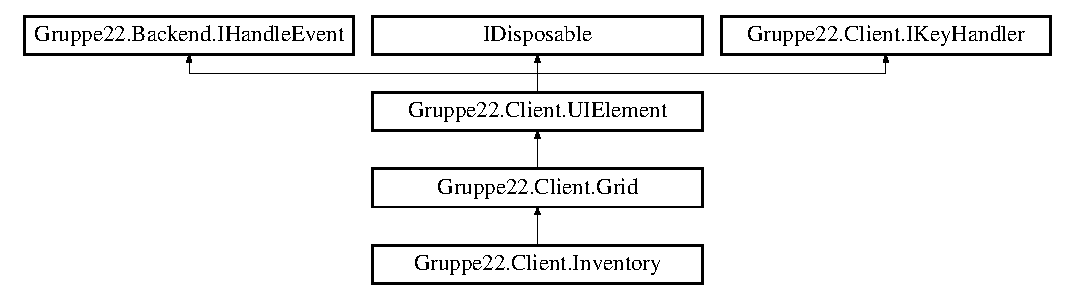
\includegraphics[height=3.589744cm]{class_gruppe22_1_1_client_1_1_inventory}
\end{center}
\end{figure}
\subsection*{Öffentliche Methoden}
\begin{DoxyCompactItemize}
\item 
void \hyperlink{class_gruppe22_1_1_client_1_1_inventory_a8dfc98c6006ae3897382f7e68b3fec67}{Update} ()
\item 
override bool \hyperlink{class_gruppe22_1_1_client_1_1_inventory_a591cf287beb11b3d2f330d8f6b812e4e}{On\-Mouse\-Down} (int button)
\begin{DoxyCompactList}\small\item\em Called when a mouse button changes from up to down \end{DoxyCompactList}\item 
\hyperlink{class_gruppe22_1_1_client_1_1_inventory_ab894c3b2a1f2985fb5714b4e3601f9b1}{Inventory} (\hyperlink{interface_gruppe22_1_1_backend_1_1_i_handle_event}{Backend.\-I\-Handle\-Event} parent, Sprite\-Batch sprite\-Batch, Content\-Manager content, Rectangle display\-Rect, \hyperlink{class_gruppe22_1_1_backend_1_1_actor}{Backend.\-Actor} \hyperlink{class_gruppe22_1_1_client_1_1_inventory_ab3465a261fd02252169362b4d110ee23}{actor}=null)
\end{DoxyCompactItemize}
\subsection*{Propertys}
\begin{DoxyCompactItemize}
\item 
\hyperlink{class_gruppe22_1_1_backend_1_1_actor}{Backend.\-Actor} \hyperlink{class_gruppe22_1_1_client_1_1_inventory_ab3465a261fd02252169362b4d110ee23}{actor}\hspace{0.3cm}{\ttfamily  \mbox{[}get, set\mbox{]}}
\end{DoxyCompactItemize}
\subsection*{Weitere Geerbte Elemente}


\subsection{Beschreibung der Konstruktoren und Destruktoren}
\hypertarget{class_gruppe22_1_1_client_1_1_inventory_ab894c3b2a1f2985fb5714b4e3601f9b1}{\index{Gruppe22\-::\-Client\-::\-Inventory@{Gruppe22\-::\-Client\-::\-Inventory}!Inventory@{Inventory}}
\index{Inventory@{Inventory}!Gruppe22::Client::Inventory@{Gruppe22\-::\-Client\-::\-Inventory}}
\subsubsection[{Inventory}]{\setlength{\rightskip}{0pt plus 5cm}Gruppe22.\-Client.\-Inventory.\-Inventory (
\begin{DoxyParamCaption}
\item[{{\bf Backend.\-I\-Handle\-Event}}]{parent, }
\item[{Sprite\-Batch}]{sprite\-Batch, }
\item[{Content\-Manager}]{content, }
\item[{Rectangle}]{display\-Rect, }
\item[{{\bf Backend.\-Actor}}]{actor = {\ttfamily null}}
\end{DoxyParamCaption}
)}}\label{class_gruppe22_1_1_client_1_1_inventory_ab894c3b2a1f2985fb5714b4e3601f9b1}


\subsection{Dokumentation der Elementfunktionen}
\hypertarget{class_gruppe22_1_1_client_1_1_inventory_a591cf287beb11b3d2f330d8f6b812e4e}{\index{Gruppe22\-::\-Client\-::\-Inventory@{Gruppe22\-::\-Client\-::\-Inventory}!On\-Mouse\-Down@{On\-Mouse\-Down}}
\index{On\-Mouse\-Down@{On\-Mouse\-Down}!Gruppe22::Client::Inventory@{Gruppe22\-::\-Client\-::\-Inventory}}
\subsubsection[{On\-Mouse\-Down}]{\setlength{\rightskip}{0pt plus 5cm}override bool Gruppe22.\-Client.\-Inventory.\-On\-Mouse\-Down (
\begin{DoxyParamCaption}
\item[{int}]{button}
\end{DoxyParamCaption}
)\hspace{0.3cm}{\ttfamily [virtual]}}}\label{class_gruppe22_1_1_client_1_1_inventory_a591cf287beb11b3d2f330d8f6b812e4e}


Called when a mouse button changes from up to down 


\begin{DoxyParams}{Parameter}
{\em button} & Left \hyperlink{class_gruppe22_1_1_client_1_1_button}{Button}=1, Middle \hyperlink{class_gruppe22_1_1_client_1_1_button}{Button}=2, Right \hyperlink{class_gruppe22_1_1_client_1_1_button}{Button}=3\\
\hline
\end{DoxyParams}


Erneute Implementation von \hyperlink{class_gruppe22_1_1_client_1_1_grid_a73b2172889aee0a3135a62c0d1af76e9}{Gruppe22.\-Client.\-Grid}.

\hypertarget{class_gruppe22_1_1_client_1_1_inventory_a8dfc98c6006ae3897382f7e68b3fec67}{\index{Gruppe22\-::\-Client\-::\-Inventory@{Gruppe22\-::\-Client\-::\-Inventory}!Update@{Update}}
\index{Update@{Update}!Gruppe22::Client::Inventory@{Gruppe22\-::\-Client\-::\-Inventory}}
\subsubsection[{Update}]{\setlength{\rightskip}{0pt plus 5cm}void Gruppe22.\-Client.\-Inventory.\-Update (
\begin{DoxyParamCaption}
{}
\end{DoxyParamCaption}
)}}\label{class_gruppe22_1_1_client_1_1_inventory_a8dfc98c6006ae3897382f7e68b3fec67}


\subsection{Dokumentation der Propertys}
\hypertarget{class_gruppe22_1_1_client_1_1_inventory_ab3465a261fd02252169362b4d110ee23}{\index{Gruppe22\-::\-Client\-::\-Inventory@{Gruppe22\-::\-Client\-::\-Inventory}!actor@{actor}}
\index{actor@{actor}!Gruppe22::Client::Inventory@{Gruppe22\-::\-Client\-::\-Inventory}}
\subsubsection[{actor}]{\setlength{\rightskip}{0pt plus 5cm}{\bf Backend.\-Actor} Gruppe22.\-Client.\-Inventory.\-actor\hspace{0.3cm}{\ttfamily [get]}, {\ttfamily [set]}}}\label{class_gruppe22_1_1_client_1_1_inventory_ab3465a261fd02252169362b4d110ee23}


Die Dokumentation für diese Klasse wurde erzeugt aufgrund der Datei\-:\begin{DoxyCompactItemize}
\item 
C\-:/\-Users/beursken/\-Documents/\-Git\-Hub/gruppe22/\-Gruppe22/\-Gruppe22/\-Client/\-U\-I/\hyperlink{_inventory_8cs}{Inventory.\-cs}\end{DoxyCompactItemize}

\hypertarget{class_gruppe22_1_1_backend_1_1_item}{\section{Gruppe22.\-Backend.\-Item Klassenreferenz}
\label{class_gruppe22_1_1_backend_1_1_item}\index{Gruppe22.\-Backend.\-Item@{Gruppe22.\-Backend.\-Item}}
}
\subsection*{Öffentliche Methoden}
\begin{DoxyCompactItemize}
\item 
virtual void \hyperlink{class_gruppe22_1_1_backend_1_1_item_a1f5cf108b31805827e61e3b258aec89a}{Equip\-Item} ()
\item 
virtual void \hyperlink{class_gruppe22_1_1_backend_1_1_item_af52b17ce2c48fadc508be98736993ad6}{Use\-Item} ()
\item 
void \hyperlink{class_gruppe22_1_1_backend_1_1_item_a884f05467df8e7171200873e3e77bee7}{Change\-Effect} (\hyperlink{class_gruppe22_1_1_backend_1_1_item_effect}{Item\-Effect} effect, bool enable)
\item 
void \hyperlink{class_gruppe22_1_1_backend_1_1_item_a0d64ac455259d3591a828979af8fc037}{Update} ()
\item 
void \hyperlink{class_gruppe22_1_1_backend_1_1_item_a45803de46f6e258be265a0cca5ddacfe}{Load} (Xml\-Reader reader)
\item 
void \hyperlink{class_gruppe22_1_1_backend_1_1_item_a9da5fe24ef57badc1d8ffa8ef41e0bdc}{Save} (Xml\-Writer xmlw)
\item 
void \hyperlink{class_gruppe22_1_1_backend_1_1_item_ae74b65ee3382bc05071469029de80864}{Generate\-Name} ()
\item 
void \hyperlink{class_gruppe22_1_1_backend_1_1_item_a0463c9e08133140294194c091b8939ea}{Estimate\-Value} ()
\item 
void \hyperlink{class_gruppe22_1_1_backend_1_1_item_a8f022dad2e31a84323153f736bf38408}{Generate\-Properties} (Random r=null)
\item 
void \hyperlink{class_gruppe22_1_1_backend_1_1_item_a1e4c5e9ec67f41f945c29734c9b383ba}{Pickup} (\hyperlink{class_gruppe22_1_1_backend_1_1_actor}{Actor} actor)
\item 
void \hyperlink{class_gruppe22_1_1_backend_1_1_item_af0ab1ef5abcf45ffe94fcb1e714c4918}{Drop} (\hyperlink{class_gruppe22_1_1_backend_1_1_floor_tile}{Floor\-Tile} \hyperlink{class_gruppe22_1_1_backend_1_1_item_ad982ec382c07e05bf4cd77c4643fc076}{tile})
\item 
void \hyperlink{class_gruppe22_1_1_backend_1_1_item_ab6ccca0c929b56e541d7115223f137fb}{Generate\-Icon} ()
\item 
\hyperlink{class_gruppe22_1_1_backend_1_1_item_a75e2fc85d059270f14988274e865b011}{Item} (Content\-Manager content, Random r=null, int \hyperlink{class_gruppe22_1_1_backend_1_1_item_a738eaf9f7acc989f8885f4973aab6804}{value}=0, int \hyperlink{class_gruppe22_1_1_backend_1_1_item_a0139f617006079f108967a3f06554f4c}{level}=1, bool gold=true)
\item 
\hyperlink{class_gruppe22_1_1_backend_1_1_item_a8032f6051a8042630607fefa60c15d25}{Item} (Content\-Manager content, \hyperlink{namespace_gruppe22_1_1_backend_ad9b2305e9d47cf46b34e082657cc5504}{Item\-Type} itemtype, string \hyperlink{class_gruppe22_1_1_backend_1_1_item_a28054626270074cd99dd99a3226d4cb6}{name}=\char`\"{}\char`\"{}, Random r=null, \hyperlink{class_gruppe22_1_1_backend_1_1_image_data}{Image\-Data} \hyperlink{class_gruppe22_1_1_backend_1_1_item_a83b9b5f8ad0469d97ff596af764f4208}{icon}=null, int \hyperlink{class_gruppe22_1_1_backend_1_1_item_a738eaf9f7acc989f8885f4973aab6804}{value}=0, int \hyperlink{class_gruppe22_1_1_backend_1_1_item_a0139f617006079f108967a3f06554f4c}{level}=1)
\item 
\hyperlink{class_gruppe22_1_1_backend_1_1_item_acc117af1ca05486c37aa84c09435750a}{Item} (Content\-Manager content, \hyperlink{class_gruppe22_1_1_backend_1_1_item_tile}{Item\-Tile} parent, \hyperlink{namespace_gruppe22_1_1_backend_ad9b2305e9d47cf46b34e082657cc5504}{Item\-Type} itemtype, string \hyperlink{class_gruppe22_1_1_backend_1_1_item_a28054626270074cd99dd99a3226d4cb6}{name}=\char`\"{}\char`\"{}, \hyperlink{class_gruppe22_1_1_backend_1_1_image_data}{Image\-Data} \hyperlink{class_gruppe22_1_1_backend_1_1_item_a83b9b5f8ad0469d97ff596af764f4208}{icon}=null, int \hyperlink{class_gruppe22_1_1_backend_1_1_item_a738eaf9f7acc989f8885f4973aab6804}{value}=0, int \hyperlink{class_gruppe22_1_1_backend_1_1_item_a0139f617006079f108967a3f06554f4c}{level}=1)
\item 
\hyperlink{class_gruppe22_1_1_backend_1_1_item_abab35be8b115d9b1078f6d57cdc32173}{Item} (Content\-Manager content, \hyperlink{class_gruppe22_1_1_backend_1_1_actor}{Actor} \hyperlink{class_gruppe22_1_1_backend_1_1_item_af11a242f1a41cad4717d05e4006b6b22}{owner}, \hyperlink{namespace_gruppe22_1_1_backend_ad9b2305e9d47cf46b34e082657cc5504}{Item\-Type} itemtype, string \hyperlink{class_gruppe22_1_1_backend_1_1_item_a28054626270074cd99dd99a3226d4cb6}{name}=\char`\"{}\char`\"{}, \hyperlink{class_gruppe22_1_1_backend_1_1_image_data}{Image\-Data} \hyperlink{class_gruppe22_1_1_backend_1_1_item_a83b9b5f8ad0469d97ff596af764f4208}{icon}=null, int \hyperlink{class_gruppe22_1_1_backend_1_1_item_a738eaf9f7acc989f8885f4973aab6804}{value}=0, int \hyperlink{class_gruppe22_1_1_backend_1_1_item_a0139f617006079f108967a3f06554f4c}{level}=1)
\item 
\hyperlink{class_gruppe22_1_1_backend_1_1_item_a78f60ea2007b781bda217db9c2a3bbf4}{Item} (Content\-Manager content)
\end{DoxyCompactItemize}
\subsection*{Öffentliche, statische Methoden}
\begin{DoxyCompactItemize}
\item 
static string \hyperlink{class_gruppe22_1_1_backend_1_1_item_a2de47879fd8a86657fbb432d530bdc5b}{Property\-To\-String} (\hyperlink{namespace_gruppe22_1_1_backend_a0bab4fb79b71059941f85a901606a7df}{Item\-Property} property)
\end{DoxyCompactItemize}
\subsection*{Propertys}
\begin{DoxyCompactItemize}
\item 
int \hyperlink{class_gruppe22_1_1_backend_1_1_item_a738eaf9f7acc989f8885f4973aab6804}{value}\hspace{0.3cm}{\ttfamily  \mbox{[}get, set\mbox{]}}
\item 
List$<$ \hyperlink{class_gruppe22_1_1_backend_1_1_item_effect}{Item\-Effect} $>$ \hyperlink{class_gruppe22_1_1_backend_1_1_item_a30f03b39159c6f65e569eb492d878f90}{effects}\hspace{0.3cm}{\ttfamily  \mbox{[}get\mbox{]}}
\item 
bool \hyperlink{class_gruppe22_1_1_backend_1_1_item_a156f66cff295f593717be085a454234d}{is\-New}\hspace{0.3cm}{\ttfamily  \mbox{[}get, set\mbox{]}}
\item 
\hyperlink{class_gruppe22_1_1_backend_1_1_actor}{Actor} \hyperlink{class_gruppe22_1_1_backend_1_1_item_af11a242f1a41cad4717d05e4006b6b22}{owner}\hspace{0.3cm}{\ttfamily  \mbox{[}get, set\mbox{]}}
\item 
int \hyperlink{class_gruppe22_1_1_backend_1_1_item_a26fab2d08c72dffe7e431182f395bc16}{id}\hspace{0.3cm}{\ttfamily  \mbox{[}get, set\mbox{]}}
\item 
int \hyperlink{class_gruppe22_1_1_backend_1_1_item_a0139f617006079f108967a3f06554f4c}{level}\hspace{0.3cm}{\ttfamily  \mbox{[}get, set\mbox{]}}
\item 
\hyperlink{class_gruppe22_1_1_backend_1_1_image_data}{Image\-Data} \hyperlink{class_gruppe22_1_1_backend_1_1_item_a83b9b5f8ad0469d97ff596af764f4208}{icon}\hspace{0.3cm}{\ttfamily  \mbox{[}get, set\mbox{]}}
\item 
bool \hyperlink{class_gruppe22_1_1_backend_1_1_item_ace7a7b499596d51df89fd10fb2c27627}{equipped}\hspace{0.3cm}{\ttfamily  \mbox{[}get, set\mbox{]}}
\item 
\hyperlink{class_gruppe22_1_1_backend_1_1_item_tile}{Item\-Tile} \hyperlink{class_gruppe22_1_1_backend_1_1_item_ad982ec382c07e05bf4cd77c4643fc076}{tile}\hspace{0.3cm}{\ttfamily  \mbox{[}get, set\mbox{]}}
\item 
bool \hyperlink{class_gruppe22_1_1_backend_1_1_item_a46fc7e28299b36877fef8d81d5a0ba9d}{destroyed}\hspace{0.3cm}{\ttfamily  \mbox{[}get, set\mbox{]}}
\item 
string \hyperlink{class_gruppe22_1_1_backend_1_1_item_a28054626270074cd99dd99a3226d4cb6}{name}\hspace{0.3cm}{\ttfamily  \mbox{[}get, set\mbox{]}}
\item 
string \hyperlink{class_gruppe22_1_1_backend_1_1_item_a1b6a2aa79d048b55e2a16e307493d300}{description}\hspace{0.3cm}{\ttfamily  \mbox{[}get, set\mbox{]}}
\item 
\hyperlink{namespace_gruppe22_1_1_backend_ad9b2305e9d47cf46b34e082657cc5504}{Item\-Type} \hyperlink{class_gruppe22_1_1_backend_1_1_item_a51bc2556416f3458650951127b277a42}{item\-Type}\hspace{0.3cm}{\ttfamily  \mbox{[}get\mbox{]}}
\item 
string \hyperlink{class_gruppe22_1_1_backend_1_1_item_a7c893ef35f4254c0ad0a192ed876224b}{ability\-List}\hspace{0.3cm}{\ttfamily  \mbox{[}get\mbox{]}}
\end{DoxyCompactItemize}


\subsection{Beschreibung der Konstruktoren und Destruktoren}
\hypertarget{class_gruppe22_1_1_backend_1_1_item_a75e2fc85d059270f14988274e865b011}{\index{Gruppe22\-::\-Backend\-::\-Item@{Gruppe22\-::\-Backend\-::\-Item}!Item@{Item}}
\index{Item@{Item}!Gruppe22::Backend::Item@{Gruppe22\-::\-Backend\-::\-Item}}
\subsubsection[{Item}]{\setlength{\rightskip}{0pt plus 5cm}Gruppe22.\-Backend.\-Item.\-Item (
\begin{DoxyParamCaption}
\item[{Content\-Manager}]{content, }
\item[{Random}]{r = {\ttfamily null}, }
\item[{int}]{value = {\ttfamily 0}, }
\item[{int}]{level = {\ttfamily 1}, }
\item[{bool}]{gold = {\ttfamily true}}
\end{DoxyParamCaption}
)}}\label{class_gruppe22_1_1_backend_1_1_item_a75e2fc85d059270f14988274e865b011}
\hypertarget{class_gruppe22_1_1_backend_1_1_item_a8032f6051a8042630607fefa60c15d25}{\index{Gruppe22\-::\-Backend\-::\-Item@{Gruppe22\-::\-Backend\-::\-Item}!Item@{Item}}
\index{Item@{Item}!Gruppe22::Backend::Item@{Gruppe22\-::\-Backend\-::\-Item}}
\subsubsection[{Item}]{\setlength{\rightskip}{0pt plus 5cm}Gruppe22.\-Backend.\-Item.\-Item (
\begin{DoxyParamCaption}
\item[{Content\-Manager}]{content, }
\item[{{\bf Item\-Type}}]{itemtype, }
\item[{string}]{name = {\ttfamily \char`\"{}\char`\"{}}, }
\item[{Random}]{r = {\ttfamily null}, }
\item[{{\bf Image\-Data}}]{icon = {\ttfamily null}, }
\item[{int}]{value = {\ttfamily 0}, }
\item[{int}]{level = {\ttfamily 1}}
\end{DoxyParamCaption}
)}}\label{class_gruppe22_1_1_backend_1_1_item_a8032f6051a8042630607fefa60c15d25}
\hypertarget{class_gruppe22_1_1_backend_1_1_item_acc117af1ca05486c37aa84c09435750a}{\index{Gruppe22\-::\-Backend\-::\-Item@{Gruppe22\-::\-Backend\-::\-Item}!Item@{Item}}
\index{Item@{Item}!Gruppe22::Backend::Item@{Gruppe22\-::\-Backend\-::\-Item}}
\subsubsection[{Item}]{\setlength{\rightskip}{0pt plus 5cm}Gruppe22.\-Backend.\-Item.\-Item (
\begin{DoxyParamCaption}
\item[{Content\-Manager}]{content, }
\item[{{\bf Item\-Tile}}]{parent, }
\item[{{\bf Item\-Type}}]{itemtype, }
\item[{string}]{name = {\ttfamily \char`\"{}\char`\"{}}, }
\item[{{\bf Image\-Data}}]{icon = {\ttfamily null}, }
\item[{int}]{value = {\ttfamily 0}, }
\item[{int}]{level = {\ttfamily 1}}
\end{DoxyParamCaption}
)}}\label{class_gruppe22_1_1_backend_1_1_item_acc117af1ca05486c37aa84c09435750a}
\hypertarget{class_gruppe22_1_1_backend_1_1_item_abab35be8b115d9b1078f6d57cdc32173}{\index{Gruppe22\-::\-Backend\-::\-Item@{Gruppe22\-::\-Backend\-::\-Item}!Item@{Item}}
\index{Item@{Item}!Gruppe22::Backend::Item@{Gruppe22\-::\-Backend\-::\-Item}}
\subsubsection[{Item}]{\setlength{\rightskip}{0pt plus 5cm}Gruppe22.\-Backend.\-Item.\-Item (
\begin{DoxyParamCaption}
\item[{Content\-Manager}]{content, }
\item[{{\bf Actor}}]{owner, }
\item[{{\bf Item\-Type}}]{itemtype, }
\item[{string}]{name = {\ttfamily \char`\"{}\char`\"{}}, }
\item[{{\bf Image\-Data}}]{icon = {\ttfamily null}, }
\item[{int}]{value = {\ttfamily 0}, }
\item[{int}]{level = {\ttfamily 1}}
\end{DoxyParamCaption}
)}}\label{class_gruppe22_1_1_backend_1_1_item_abab35be8b115d9b1078f6d57cdc32173}
\hypertarget{class_gruppe22_1_1_backend_1_1_item_a78f60ea2007b781bda217db9c2a3bbf4}{\index{Gruppe22\-::\-Backend\-::\-Item@{Gruppe22\-::\-Backend\-::\-Item}!Item@{Item}}
\index{Item@{Item}!Gruppe22::Backend::Item@{Gruppe22\-::\-Backend\-::\-Item}}
\subsubsection[{Item}]{\setlength{\rightskip}{0pt plus 5cm}Gruppe22.\-Backend.\-Item.\-Item (
\begin{DoxyParamCaption}
\item[{Content\-Manager}]{content}
\end{DoxyParamCaption}
)}}\label{class_gruppe22_1_1_backend_1_1_item_a78f60ea2007b781bda217db9c2a3bbf4}


\subsection{Dokumentation der Elementfunktionen}
\hypertarget{class_gruppe22_1_1_backend_1_1_item_a884f05467df8e7171200873e3e77bee7}{\index{Gruppe22\-::\-Backend\-::\-Item@{Gruppe22\-::\-Backend\-::\-Item}!Change\-Effect@{Change\-Effect}}
\index{Change\-Effect@{Change\-Effect}!Gruppe22::Backend::Item@{Gruppe22\-::\-Backend\-::\-Item}}
\subsubsection[{Change\-Effect}]{\setlength{\rightskip}{0pt plus 5cm}void Gruppe22.\-Backend.\-Item.\-Change\-Effect (
\begin{DoxyParamCaption}
\item[{{\bf Item\-Effect}}]{effect, }
\item[{bool}]{enable}
\end{DoxyParamCaption}
)}}\label{class_gruppe22_1_1_backend_1_1_item_a884f05467df8e7171200873e3e77bee7}
\hypertarget{class_gruppe22_1_1_backend_1_1_item_af0ab1ef5abcf45ffe94fcb1e714c4918}{\index{Gruppe22\-::\-Backend\-::\-Item@{Gruppe22\-::\-Backend\-::\-Item}!Drop@{Drop}}
\index{Drop@{Drop}!Gruppe22::Backend::Item@{Gruppe22\-::\-Backend\-::\-Item}}
\subsubsection[{Drop}]{\setlength{\rightskip}{0pt plus 5cm}void Gruppe22.\-Backend.\-Item.\-Drop (
\begin{DoxyParamCaption}
\item[{{\bf Floor\-Tile}}]{tile}
\end{DoxyParamCaption}
)}}\label{class_gruppe22_1_1_backend_1_1_item_af0ab1ef5abcf45ffe94fcb1e714c4918}
\hypertarget{class_gruppe22_1_1_backend_1_1_item_a1f5cf108b31805827e61e3b258aec89a}{\index{Gruppe22\-::\-Backend\-::\-Item@{Gruppe22\-::\-Backend\-::\-Item}!Equip\-Item@{Equip\-Item}}
\index{Equip\-Item@{Equip\-Item}!Gruppe22::Backend::Item@{Gruppe22\-::\-Backend\-::\-Item}}
\subsubsection[{Equip\-Item}]{\setlength{\rightskip}{0pt plus 5cm}virtual void Gruppe22.\-Backend.\-Item.\-Equip\-Item (
\begin{DoxyParamCaption}
{}
\end{DoxyParamCaption}
)\hspace{0.3cm}{\ttfamily [virtual]}}}\label{class_gruppe22_1_1_backend_1_1_item_a1f5cf108b31805827e61e3b258aec89a}
\hypertarget{class_gruppe22_1_1_backend_1_1_item_a0463c9e08133140294194c091b8939ea}{\index{Gruppe22\-::\-Backend\-::\-Item@{Gruppe22\-::\-Backend\-::\-Item}!Estimate\-Value@{Estimate\-Value}}
\index{Estimate\-Value@{Estimate\-Value}!Gruppe22::Backend::Item@{Gruppe22\-::\-Backend\-::\-Item}}
\subsubsection[{Estimate\-Value}]{\setlength{\rightskip}{0pt plus 5cm}void Gruppe22.\-Backend.\-Item.\-Estimate\-Value (
\begin{DoxyParamCaption}
{}
\end{DoxyParamCaption}
)}}\label{class_gruppe22_1_1_backend_1_1_item_a0463c9e08133140294194c091b8939ea}
\hypertarget{class_gruppe22_1_1_backend_1_1_item_ab6ccca0c929b56e541d7115223f137fb}{\index{Gruppe22\-::\-Backend\-::\-Item@{Gruppe22\-::\-Backend\-::\-Item}!Generate\-Icon@{Generate\-Icon}}
\index{Generate\-Icon@{Generate\-Icon}!Gruppe22::Backend::Item@{Gruppe22\-::\-Backend\-::\-Item}}
\subsubsection[{Generate\-Icon}]{\setlength{\rightskip}{0pt plus 5cm}void Gruppe22.\-Backend.\-Item.\-Generate\-Icon (
\begin{DoxyParamCaption}
{}
\end{DoxyParamCaption}
)}}\label{class_gruppe22_1_1_backend_1_1_item_ab6ccca0c929b56e541d7115223f137fb}
\hypertarget{class_gruppe22_1_1_backend_1_1_item_ae74b65ee3382bc05071469029de80864}{\index{Gruppe22\-::\-Backend\-::\-Item@{Gruppe22\-::\-Backend\-::\-Item}!Generate\-Name@{Generate\-Name}}
\index{Generate\-Name@{Generate\-Name}!Gruppe22::Backend::Item@{Gruppe22\-::\-Backend\-::\-Item}}
\subsubsection[{Generate\-Name}]{\setlength{\rightskip}{0pt plus 5cm}void Gruppe22.\-Backend.\-Item.\-Generate\-Name (
\begin{DoxyParamCaption}
{}
\end{DoxyParamCaption}
)}}\label{class_gruppe22_1_1_backend_1_1_item_ae74b65ee3382bc05071469029de80864}
\hypertarget{class_gruppe22_1_1_backend_1_1_item_a8f022dad2e31a84323153f736bf38408}{\index{Gruppe22\-::\-Backend\-::\-Item@{Gruppe22\-::\-Backend\-::\-Item}!Generate\-Properties@{Generate\-Properties}}
\index{Generate\-Properties@{Generate\-Properties}!Gruppe22::Backend::Item@{Gruppe22\-::\-Backend\-::\-Item}}
\subsubsection[{Generate\-Properties}]{\setlength{\rightskip}{0pt plus 5cm}void Gruppe22.\-Backend.\-Item.\-Generate\-Properties (
\begin{DoxyParamCaption}
\item[{Random}]{r = {\ttfamily null}}
\end{DoxyParamCaption}
)}}\label{class_gruppe22_1_1_backend_1_1_item_a8f022dad2e31a84323153f736bf38408}
\hypertarget{class_gruppe22_1_1_backend_1_1_item_a45803de46f6e258be265a0cca5ddacfe}{\index{Gruppe22\-::\-Backend\-::\-Item@{Gruppe22\-::\-Backend\-::\-Item}!Load@{Load}}
\index{Load@{Load}!Gruppe22::Backend::Item@{Gruppe22\-::\-Backend\-::\-Item}}
\subsubsection[{Load}]{\setlength{\rightskip}{0pt plus 5cm}void Gruppe22.\-Backend.\-Item.\-Load (
\begin{DoxyParamCaption}
\item[{Xml\-Reader}]{reader}
\end{DoxyParamCaption}
)}}\label{class_gruppe22_1_1_backend_1_1_item_a45803de46f6e258be265a0cca5ddacfe}
\hypertarget{class_gruppe22_1_1_backend_1_1_item_a1e4c5e9ec67f41f945c29734c9b383ba}{\index{Gruppe22\-::\-Backend\-::\-Item@{Gruppe22\-::\-Backend\-::\-Item}!Pickup@{Pickup}}
\index{Pickup@{Pickup}!Gruppe22::Backend::Item@{Gruppe22\-::\-Backend\-::\-Item}}
\subsubsection[{Pickup}]{\setlength{\rightskip}{0pt plus 5cm}void Gruppe22.\-Backend.\-Item.\-Pickup (
\begin{DoxyParamCaption}
\item[{{\bf Actor}}]{actor}
\end{DoxyParamCaption}
)}}\label{class_gruppe22_1_1_backend_1_1_item_a1e4c5e9ec67f41f945c29734c9b383ba}
\hypertarget{class_gruppe22_1_1_backend_1_1_item_a2de47879fd8a86657fbb432d530bdc5b}{\index{Gruppe22\-::\-Backend\-::\-Item@{Gruppe22\-::\-Backend\-::\-Item}!Property\-To\-String@{Property\-To\-String}}
\index{Property\-To\-String@{Property\-To\-String}!Gruppe22::Backend::Item@{Gruppe22\-::\-Backend\-::\-Item}}
\subsubsection[{Property\-To\-String}]{\setlength{\rightskip}{0pt plus 5cm}static string Gruppe22.\-Backend.\-Item.\-Property\-To\-String (
\begin{DoxyParamCaption}
\item[{{\bf Item\-Property}}]{property}
\end{DoxyParamCaption}
)\hspace{0.3cm}{\ttfamily [static]}}}\label{class_gruppe22_1_1_backend_1_1_item_a2de47879fd8a86657fbb432d530bdc5b}
\hypertarget{class_gruppe22_1_1_backend_1_1_item_a9da5fe24ef57badc1d8ffa8ef41e0bdc}{\index{Gruppe22\-::\-Backend\-::\-Item@{Gruppe22\-::\-Backend\-::\-Item}!Save@{Save}}
\index{Save@{Save}!Gruppe22::Backend::Item@{Gruppe22\-::\-Backend\-::\-Item}}
\subsubsection[{Save}]{\setlength{\rightskip}{0pt plus 5cm}void Gruppe22.\-Backend.\-Item.\-Save (
\begin{DoxyParamCaption}
\item[{Xml\-Writer}]{xmlw}
\end{DoxyParamCaption}
)}}\label{class_gruppe22_1_1_backend_1_1_item_a9da5fe24ef57badc1d8ffa8ef41e0bdc}
\hypertarget{class_gruppe22_1_1_backend_1_1_item_a0d64ac455259d3591a828979af8fc037}{\index{Gruppe22\-::\-Backend\-::\-Item@{Gruppe22\-::\-Backend\-::\-Item}!Update@{Update}}
\index{Update@{Update}!Gruppe22::Backend::Item@{Gruppe22\-::\-Backend\-::\-Item}}
\subsubsection[{Update}]{\setlength{\rightskip}{0pt plus 5cm}void Gruppe22.\-Backend.\-Item.\-Update (
\begin{DoxyParamCaption}
{}
\end{DoxyParamCaption}
)}}\label{class_gruppe22_1_1_backend_1_1_item_a0d64ac455259d3591a828979af8fc037}
\hypertarget{class_gruppe22_1_1_backend_1_1_item_af52b17ce2c48fadc508be98736993ad6}{\index{Gruppe22\-::\-Backend\-::\-Item@{Gruppe22\-::\-Backend\-::\-Item}!Use\-Item@{Use\-Item}}
\index{Use\-Item@{Use\-Item}!Gruppe22::Backend::Item@{Gruppe22\-::\-Backend\-::\-Item}}
\subsubsection[{Use\-Item}]{\setlength{\rightskip}{0pt plus 5cm}virtual void Gruppe22.\-Backend.\-Item.\-Use\-Item (
\begin{DoxyParamCaption}
{}
\end{DoxyParamCaption}
)\hspace{0.3cm}{\ttfamily [virtual]}}}\label{class_gruppe22_1_1_backend_1_1_item_af52b17ce2c48fadc508be98736993ad6}


\subsection{Dokumentation der Propertys}
\hypertarget{class_gruppe22_1_1_backend_1_1_item_a7c893ef35f4254c0ad0a192ed876224b}{\index{Gruppe22\-::\-Backend\-::\-Item@{Gruppe22\-::\-Backend\-::\-Item}!ability\-List@{ability\-List}}
\index{ability\-List@{ability\-List}!Gruppe22::Backend::Item@{Gruppe22\-::\-Backend\-::\-Item}}
\subsubsection[{ability\-List}]{\setlength{\rightskip}{0pt plus 5cm}string Gruppe22.\-Backend.\-Item.\-ability\-List\hspace{0.3cm}{\ttfamily [get]}}}\label{class_gruppe22_1_1_backend_1_1_item_a7c893ef35f4254c0ad0a192ed876224b}
\hypertarget{class_gruppe22_1_1_backend_1_1_item_a1b6a2aa79d048b55e2a16e307493d300}{\index{Gruppe22\-::\-Backend\-::\-Item@{Gruppe22\-::\-Backend\-::\-Item}!description@{description}}
\index{description@{description}!Gruppe22::Backend::Item@{Gruppe22\-::\-Backend\-::\-Item}}
\subsubsection[{description}]{\setlength{\rightskip}{0pt plus 5cm}string Gruppe22.\-Backend.\-Item.\-description\hspace{0.3cm}{\ttfamily [get]}, {\ttfamily [set]}}}\label{class_gruppe22_1_1_backend_1_1_item_a1b6a2aa79d048b55e2a16e307493d300}
\hypertarget{class_gruppe22_1_1_backend_1_1_item_a46fc7e28299b36877fef8d81d5a0ba9d}{\index{Gruppe22\-::\-Backend\-::\-Item@{Gruppe22\-::\-Backend\-::\-Item}!destroyed@{destroyed}}
\index{destroyed@{destroyed}!Gruppe22::Backend::Item@{Gruppe22\-::\-Backend\-::\-Item}}
\subsubsection[{destroyed}]{\setlength{\rightskip}{0pt plus 5cm}bool Gruppe22.\-Backend.\-Item.\-destroyed\hspace{0.3cm}{\ttfamily [get]}, {\ttfamily [set]}}}\label{class_gruppe22_1_1_backend_1_1_item_a46fc7e28299b36877fef8d81d5a0ba9d}
\hypertarget{class_gruppe22_1_1_backend_1_1_item_a30f03b39159c6f65e569eb492d878f90}{\index{Gruppe22\-::\-Backend\-::\-Item@{Gruppe22\-::\-Backend\-::\-Item}!effects@{effects}}
\index{effects@{effects}!Gruppe22::Backend::Item@{Gruppe22\-::\-Backend\-::\-Item}}
\subsubsection[{effects}]{\setlength{\rightskip}{0pt plus 5cm}List$<${\bf Item\-Effect}$>$ Gruppe22.\-Backend.\-Item.\-effects\hspace{0.3cm}{\ttfamily [get]}}}\label{class_gruppe22_1_1_backend_1_1_item_a30f03b39159c6f65e569eb492d878f90}
\hypertarget{class_gruppe22_1_1_backend_1_1_item_ace7a7b499596d51df89fd10fb2c27627}{\index{Gruppe22\-::\-Backend\-::\-Item@{Gruppe22\-::\-Backend\-::\-Item}!equipped@{equipped}}
\index{equipped@{equipped}!Gruppe22::Backend::Item@{Gruppe22\-::\-Backend\-::\-Item}}
\subsubsection[{equipped}]{\setlength{\rightskip}{0pt plus 5cm}bool Gruppe22.\-Backend.\-Item.\-equipped\hspace{0.3cm}{\ttfamily [get]}, {\ttfamily [set]}}}\label{class_gruppe22_1_1_backend_1_1_item_ace7a7b499596d51df89fd10fb2c27627}
\hypertarget{class_gruppe22_1_1_backend_1_1_item_a83b9b5f8ad0469d97ff596af764f4208}{\index{Gruppe22\-::\-Backend\-::\-Item@{Gruppe22\-::\-Backend\-::\-Item}!icon@{icon}}
\index{icon@{icon}!Gruppe22::Backend::Item@{Gruppe22\-::\-Backend\-::\-Item}}
\subsubsection[{icon}]{\setlength{\rightskip}{0pt plus 5cm}{\bf Image\-Data} Gruppe22.\-Backend.\-Item.\-icon\hspace{0.3cm}{\ttfamily [get]}, {\ttfamily [set]}}}\label{class_gruppe22_1_1_backend_1_1_item_a83b9b5f8ad0469d97ff596af764f4208}
\hypertarget{class_gruppe22_1_1_backend_1_1_item_a26fab2d08c72dffe7e431182f395bc16}{\index{Gruppe22\-::\-Backend\-::\-Item@{Gruppe22\-::\-Backend\-::\-Item}!id@{id}}
\index{id@{id}!Gruppe22::Backend::Item@{Gruppe22\-::\-Backend\-::\-Item}}
\subsubsection[{id}]{\setlength{\rightskip}{0pt plus 5cm}int Gruppe22.\-Backend.\-Item.\-id\hspace{0.3cm}{\ttfamily [get]}, {\ttfamily [set]}}}\label{class_gruppe22_1_1_backend_1_1_item_a26fab2d08c72dffe7e431182f395bc16}
\hypertarget{class_gruppe22_1_1_backend_1_1_item_a156f66cff295f593717be085a454234d}{\index{Gruppe22\-::\-Backend\-::\-Item@{Gruppe22\-::\-Backend\-::\-Item}!is\-New@{is\-New}}
\index{is\-New@{is\-New}!Gruppe22::Backend::Item@{Gruppe22\-::\-Backend\-::\-Item}}
\subsubsection[{is\-New}]{\setlength{\rightskip}{0pt plus 5cm}bool Gruppe22.\-Backend.\-Item.\-is\-New\hspace{0.3cm}{\ttfamily [get]}, {\ttfamily [set]}}}\label{class_gruppe22_1_1_backend_1_1_item_a156f66cff295f593717be085a454234d}
\hypertarget{class_gruppe22_1_1_backend_1_1_item_a51bc2556416f3458650951127b277a42}{\index{Gruppe22\-::\-Backend\-::\-Item@{Gruppe22\-::\-Backend\-::\-Item}!item\-Type@{item\-Type}}
\index{item\-Type@{item\-Type}!Gruppe22::Backend::Item@{Gruppe22\-::\-Backend\-::\-Item}}
\subsubsection[{item\-Type}]{\setlength{\rightskip}{0pt plus 5cm}{\bf Item\-Type} Gruppe22.\-Backend.\-Item.\-item\-Type\hspace{0.3cm}{\ttfamily [get]}}}\label{class_gruppe22_1_1_backend_1_1_item_a51bc2556416f3458650951127b277a42}
\hypertarget{class_gruppe22_1_1_backend_1_1_item_a0139f617006079f108967a3f06554f4c}{\index{Gruppe22\-::\-Backend\-::\-Item@{Gruppe22\-::\-Backend\-::\-Item}!level@{level}}
\index{level@{level}!Gruppe22::Backend::Item@{Gruppe22\-::\-Backend\-::\-Item}}
\subsubsection[{level}]{\setlength{\rightskip}{0pt plus 5cm}int Gruppe22.\-Backend.\-Item.\-level\hspace{0.3cm}{\ttfamily [get]}, {\ttfamily [set]}}}\label{class_gruppe22_1_1_backend_1_1_item_a0139f617006079f108967a3f06554f4c}
\hypertarget{class_gruppe22_1_1_backend_1_1_item_a28054626270074cd99dd99a3226d4cb6}{\index{Gruppe22\-::\-Backend\-::\-Item@{Gruppe22\-::\-Backend\-::\-Item}!name@{name}}
\index{name@{name}!Gruppe22::Backend::Item@{Gruppe22\-::\-Backend\-::\-Item}}
\subsubsection[{name}]{\setlength{\rightskip}{0pt plus 5cm}string Gruppe22.\-Backend.\-Item.\-name\hspace{0.3cm}{\ttfamily [get]}, {\ttfamily [set]}}}\label{class_gruppe22_1_1_backend_1_1_item_a28054626270074cd99dd99a3226d4cb6}
\hypertarget{class_gruppe22_1_1_backend_1_1_item_af11a242f1a41cad4717d05e4006b6b22}{\index{Gruppe22\-::\-Backend\-::\-Item@{Gruppe22\-::\-Backend\-::\-Item}!owner@{owner}}
\index{owner@{owner}!Gruppe22::Backend::Item@{Gruppe22\-::\-Backend\-::\-Item}}
\subsubsection[{owner}]{\setlength{\rightskip}{0pt plus 5cm}{\bf Actor} Gruppe22.\-Backend.\-Item.\-owner\hspace{0.3cm}{\ttfamily [get]}, {\ttfamily [set]}}}\label{class_gruppe22_1_1_backend_1_1_item_af11a242f1a41cad4717d05e4006b6b22}
\hypertarget{class_gruppe22_1_1_backend_1_1_item_ad982ec382c07e05bf4cd77c4643fc076}{\index{Gruppe22\-::\-Backend\-::\-Item@{Gruppe22\-::\-Backend\-::\-Item}!tile@{tile}}
\index{tile@{tile}!Gruppe22::Backend::Item@{Gruppe22\-::\-Backend\-::\-Item}}
\subsubsection[{tile}]{\setlength{\rightskip}{0pt plus 5cm}{\bf Item\-Tile} Gruppe22.\-Backend.\-Item.\-tile\hspace{0.3cm}{\ttfamily [get]}, {\ttfamily [set]}}}\label{class_gruppe22_1_1_backend_1_1_item_ad982ec382c07e05bf4cd77c4643fc076}
\hypertarget{class_gruppe22_1_1_backend_1_1_item_a738eaf9f7acc989f8885f4973aab6804}{\index{Gruppe22\-::\-Backend\-::\-Item@{Gruppe22\-::\-Backend\-::\-Item}!value@{value}}
\index{value@{value}!Gruppe22::Backend::Item@{Gruppe22\-::\-Backend\-::\-Item}}
\subsubsection[{value}]{\setlength{\rightskip}{0pt plus 5cm}int Gruppe22.\-Backend.\-Item.\-value\hspace{0.3cm}{\ttfamily [get]}, {\ttfamily [set]}}}\label{class_gruppe22_1_1_backend_1_1_item_a738eaf9f7acc989f8885f4973aab6804}


Die Dokumentation für diese Klasse wurde erzeugt aufgrund der Datei\-:\begin{DoxyCompactItemize}
\item 
C\-:/\-Users/beursken/\-Documents/\-Git\-Hub/gruppe22/\-Gruppe22/\-Gruppe22/\-Backend/\-Items/\hyperlink{_item_8cs}{Item.\-cs}\end{DoxyCompactItemize}

\hypertarget{class_gruppe22_1_1_backend_1_1_item_effect}{\section{Gruppe22.\-Backend.\-Item\-Effect Klassenreferenz}
\label{class_gruppe22_1_1_backend_1_1_item_effect}\index{Gruppe22.\-Backend.\-Item\-Effect@{Gruppe22.\-Backend.\-Item\-Effect}}
}


Effect of an item on a certain character statistic  


\subsection*{Öffentliche Methoden}
\begin{DoxyCompactItemize}
\item 
\hyperlink{class_gruppe22_1_1_backend_1_1_item_effect_a45389f27d8537fa7ff9adef341a53d16}{Item\-Effect} (\hyperlink{namespace_gruppe22_1_1_backend_a0bab4fb79b71059941f85a901606a7df}{Item\-Property} \hyperlink{class_gruppe22_1_1_backend_1_1_item_effect_ac58e4514f7c82e466da52ca6b03925cd}{property}=Item\-Property.\-Null, int \hyperlink{class_gruppe22_1_1_backend_1_1_item_effect_a9b6897a13e8e7b82698a90c4164d7ad4}{effect}=0, int \hyperlink{class_gruppe22_1_1_backend_1_1_item_effect_ae7de32850a9a94a778eae3155e39add0}{duration}=0)
\end{DoxyCompactItemize}
\subsection*{Propertys}
\begin{DoxyCompactItemize}
\item 
int \hyperlink{class_gruppe22_1_1_backend_1_1_item_effect_a9b6897a13e8e7b82698a90c4164d7ad4}{effect}\hspace{0.3cm}{\ttfamily  \mbox{[}get, set\mbox{]}}
\item 
\hyperlink{namespace_gruppe22_1_1_backend_a0bab4fb79b71059941f85a901606a7df}{Item\-Property} \hyperlink{class_gruppe22_1_1_backend_1_1_item_effect_ac58e4514f7c82e466da52ca6b03925cd}{property}\hspace{0.3cm}{\ttfamily  \mbox{[}get, set\mbox{]}}
\item 
int \hyperlink{class_gruppe22_1_1_backend_1_1_item_effect_ae7de32850a9a94a778eae3155e39add0}{duration}\hspace{0.3cm}{\ttfamily  \mbox{[}get, set\mbox{]}}
\end{DoxyCompactItemize}


\subsection{Ausführliche Beschreibung}
Effect of an item on a certain character statistic 



\subsection{Beschreibung der Konstruktoren und Destruktoren}
\hypertarget{class_gruppe22_1_1_backend_1_1_item_effect_a45389f27d8537fa7ff9adef341a53d16}{\index{Gruppe22\-::\-Backend\-::\-Item\-Effect@{Gruppe22\-::\-Backend\-::\-Item\-Effect}!Item\-Effect@{Item\-Effect}}
\index{Item\-Effect@{Item\-Effect}!Gruppe22::Backend::ItemEffect@{Gruppe22\-::\-Backend\-::\-Item\-Effect}}
\subsubsection[{Item\-Effect}]{\setlength{\rightskip}{0pt plus 5cm}Gruppe22.\-Backend.\-Item\-Effect.\-Item\-Effect (
\begin{DoxyParamCaption}
\item[{{\bf Item\-Property}}]{property = {\ttfamily ItemProperty.Null}, }
\item[{int}]{effect = {\ttfamily 0}, }
\item[{int}]{duration = {\ttfamily 0}}
\end{DoxyParamCaption}
)}}\label{class_gruppe22_1_1_backend_1_1_item_effect_a45389f27d8537fa7ff9adef341a53d16}


\subsection{Dokumentation der Propertys}
\hypertarget{class_gruppe22_1_1_backend_1_1_item_effect_ae7de32850a9a94a778eae3155e39add0}{\index{Gruppe22\-::\-Backend\-::\-Item\-Effect@{Gruppe22\-::\-Backend\-::\-Item\-Effect}!duration@{duration}}
\index{duration@{duration}!Gruppe22::Backend::ItemEffect@{Gruppe22\-::\-Backend\-::\-Item\-Effect}}
\subsubsection[{duration}]{\setlength{\rightskip}{0pt plus 5cm}int Gruppe22.\-Backend.\-Item\-Effect.\-duration\hspace{0.3cm}{\ttfamily [get]}, {\ttfamily [set]}}}\label{class_gruppe22_1_1_backend_1_1_item_effect_ae7de32850a9a94a778eae3155e39add0}
\hypertarget{class_gruppe22_1_1_backend_1_1_item_effect_a9b6897a13e8e7b82698a90c4164d7ad4}{\index{Gruppe22\-::\-Backend\-::\-Item\-Effect@{Gruppe22\-::\-Backend\-::\-Item\-Effect}!effect@{effect}}
\index{effect@{effect}!Gruppe22::Backend::ItemEffect@{Gruppe22\-::\-Backend\-::\-Item\-Effect}}
\subsubsection[{effect}]{\setlength{\rightskip}{0pt plus 5cm}int Gruppe22.\-Backend.\-Item\-Effect.\-effect\hspace{0.3cm}{\ttfamily [get]}, {\ttfamily [set]}}}\label{class_gruppe22_1_1_backend_1_1_item_effect_a9b6897a13e8e7b82698a90c4164d7ad4}
\hypertarget{class_gruppe22_1_1_backend_1_1_item_effect_ac58e4514f7c82e466da52ca6b03925cd}{\index{Gruppe22\-::\-Backend\-::\-Item\-Effect@{Gruppe22\-::\-Backend\-::\-Item\-Effect}!property@{property}}
\index{property@{property}!Gruppe22::Backend::ItemEffect@{Gruppe22\-::\-Backend\-::\-Item\-Effect}}
\subsubsection[{property}]{\setlength{\rightskip}{0pt plus 5cm}{\bf Item\-Property} Gruppe22.\-Backend.\-Item\-Effect.\-property\hspace{0.3cm}{\ttfamily [get]}, {\ttfamily [set]}}}\label{class_gruppe22_1_1_backend_1_1_item_effect_ac58e4514f7c82e466da52ca6b03925cd}


Die Dokumentation für diese Klasse wurde erzeugt aufgrund der Datei\-:\begin{DoxyCompactItemize}
\item 
C\-:/\-Users/beursken/\-Documents/\-Git\-Hub/gruppe22/\-Gruppe22/\-Gruppe22/\-Backend/\-Items/\hyperlink{_item_effect_8cs}{Item\-Effect.\-cs}\end{DoxyCompactItemize}

\hypertarget{class_gruppe22_1_1_backend_1_1_item_tile}{\section{Gruppe22.\-Backend.\-Item\-Tile Klassenreferenz}
\label{class_gruppe22_1_1_backend_1_1_item_tile}\index{Gruppe22.\-Backend.\-Item\-Tile@{Gruppe22.\-Backend.\-Item\-Tile}}
}
Klassendiagramm für Gruppe22.\-Backend.\-Item\-Tile\-:\begin{figure}[H]
\begin{center}
\leavevmode
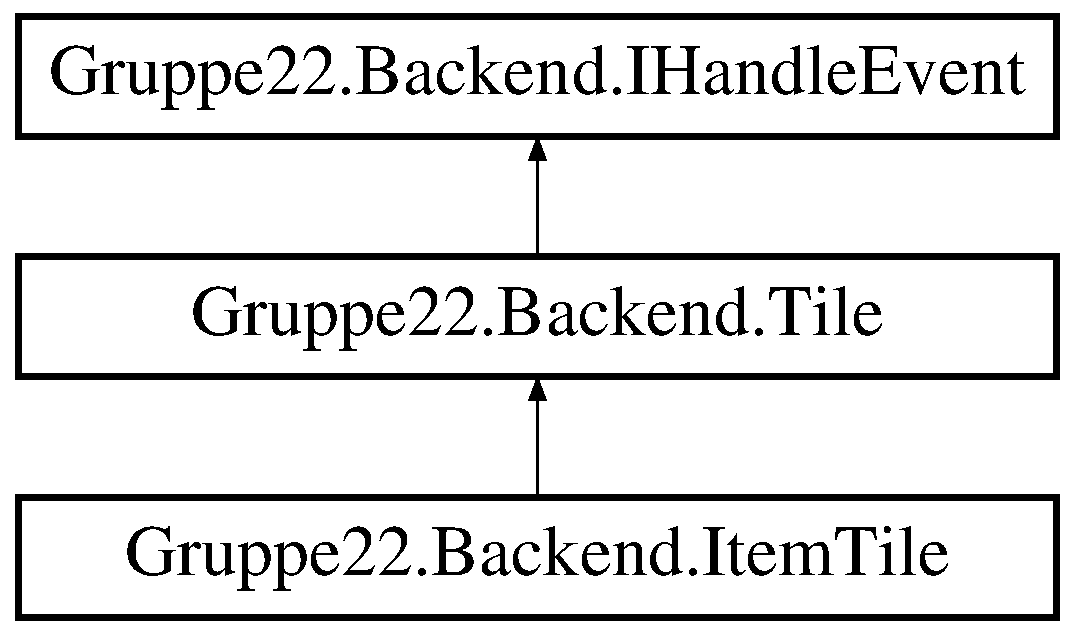
\includegraphics[height=3.000000cm]{class_gruppe22_1_1_backend_1_1_item_tile}
\end{center}
\end{figure}
\subsection*{Öffentliche Methoden}
\begin{DoxyCompactItemize}
\item 
override void \hyperlink{class_gruppe22_1_1_backend_1_1_item_tile_a2e58e18ae35c42b311fcdaa1664ec505}{Save} (Xml\-Writer xmlw)
\begin{DoxyCompactList}\small\item\em Abstract method to save a tile in a X\-M\-L file \end{DoxyCompactList}\item 
\hyperlink{class_gruppe22_1_1_backend_1_1_item_tile_a7975720b4b34cb910403f8ead9caae56}{Item\-Tile} (object \hyperlink{class_gruppe22_1_1_backend_1_1_tile_abc12933c70eb3a2ebbb2fde9f45c2632}{parent}, \hyperlink{class_gruppe22_1_1_backend_1_1_item}{Item} \hyperlink{class_gruppe22_1_1_backend_1_1_item_tile_a1c70024d6768af2fbeeb988fc14838be}{item})
\item 
\hyperlink{class_gruppe22_1_1_backend_1_1_item_tile_a0fd464405cb497015bee896ab1d389d8}{Item\-Tile} (object \hyperlink{class_gruppe22_1_1_backend_1_1_tile_abc12933c70eb3a2ebbb2fde9f45c2632}{parent})
\end{DoxyCompactItemize}
\subsection*{Propertys}
\begin{DoxyCompactItemize}
\item 
\hyperlink{class_gruppe22_1_1_backend_1_1_item}{Item} \hyperlink{class_gruppe22_1_1_backend_1_1_item_tile_a1c70024d6768af2fbeeb988fc14838be}{item}\hspace{0.3cm}{\ttfamily  \mbox{[}get, set\mbox{]}}
\item 
\hyperlink{namespace_gruppe22_1_1_backend_ad9b2305e9d47cf46b34e082657cc5504}{Item\-Type} \hyperlink{class_gruppe22_1_1_backend_1_1_item_tile_a2bda4d14a172ae8b2b7c66c9d2b67c85}{item\-Type}\hspace{0.3cm}{\ttfamily  \mbox{[}get\mbox{]}}
\end{DoxyCompactItemize}
\subsection*{Weitere Geerbte Elemente}


\subsection{Beschreibung der Konstruktoren und Destruktoren}
\hypertarget{class_gruppe22_1_1_backend_1_1_item_tile_a7975720b4b34cb910403f8ead9caae56}{\index{Gruppe22\-::\-Backend\-::\-Item\-Tile@{Gruppe22\-::\-Backend\-::\-Item\-Tile}!Item\-Tile@{Item\-Tile}}
\index{Item\-Tile@{Item\-Tile}!Gruppe22::Backend::ItemTile@{Gruppe22\-::\-Backend\-::\-Item\-Tile}}
\subsubsection[{Item\-Tile}]{\setlength{\rightskip}{0pt plus 5cm}Gruppe22.\-Backend.\-Item\-Tile.\-Item\-Tile (
\begin{DoxyParamCaption}
\item[{object}]{parent, }
\item[{{\bf Item}}]{item}
\end{DoxyParamCaption}
)}}\label{class_gruppe22_1_1_backend_1_1_item_tile_a7975720b4b34cb910403f8ead9caae56}
\hypertarget{class_gruppe22_1_1_backend_1_1_item_tile_a0fd464405cb497015bee896ab1d389d8}{\index{Gruppe22\-::\-Backend\-::\-Item\-Tile@{Gruppe22\-::\-Backend\-::\-Item\-Tile}!Item\-Tile@{Item\-Tile}}
\index{Item\-Tile@{Item\-Tile}!Gruppe22::Backend::ItemTile@{Gruppe22\-::\-Backend\-::\-Item\-Tile}}
\subsubsection[{Item\-Tile}]{\setlength{\rightskip}{0pt plus 5cm}Gruppe22.\-Backend.\-Item\-Tile.\-Item\-Tile (
\begin{DoxyParamCaption}
\item[{object}]{parent}
\end{DoxyParamCaption}
)}}\label{class_gruppe22_1_1_backend_1_1_item_tile_a0fd464405cb497015bee896ab1d389d8}


\subsection{Dokumentation der Elementfunktionen}
\hypertarget{class_gruppe22_1_1_backend_1_1_item_tile_a2e58e18ae35c42b311fcdaa1664ec505}{\index{Gruppe22\-::\-Backend\-::\-Item\-Tile@{Gruppe22\-::\-Backend\-::\-Item\-Tile}!Save@{Save}}
\index{Save@{Save}!Gruppe22::Backend::ItemTile@{Gruppe22\-::\-Backend\-::\-Item\-Tile}}
\subsubsection[{Save}]{\setlength{\rightskip}{0pt plus 5cm}override void Gruppe22.\-Backend.\-Item\-Tile.\-Save (
\begin{DoxyParamCaption}
\item[{Xml\-Writer}]{xmlw}
\end{DoxyParamCaption}
)\hspace{0.3cm}{\ttfamily [virtual]}}}\label{class_gruppe22_1_1_backend_1_1_item_tile_a2e58e18ae35c42b311fcdaa1664ec505}


Abstract method to save a tile in a X\-M\-L file 


\begin{DoxyParams}{Parameter}
{\em xmlw} & the Xml\-Writer used for saving the file\\
\hline
\end{DoxyParams}


Erneute Implementation von \hyperlink{class_gruppe22_1_1_backend_1_1_tile_a109ab3e77ffca9d44c95a711af3491dc}{Gruppe22.\-Backend.\-Tile}.



\subsection{Dokumentation der Propertys}
\hypertarget{class_gruppe22_1_1_backend_1_1_item_tile_a1c70024d6768af2fbeeb988fc14838be}{\index{Gruppe22\-::\-Backend\-::\-Item\-Tile@{Gruppe22\-::\-Backend\-::\-Item\-Tile}!item@{item}}
\index{item@{item}!Gruppe22::Backend::ItemTile@{Gruppe22\-::\-Backend\-::\-Item\-Tile}}
\subsubsection[{item}]{\setlength{\rightskip}{0pt plus 5cm}{\bf Item} Gruppe22.\-Backend.\-Item\-Tile.\-item\hspace{0.3cm}{\ttfamily [get]}, {\ttfamily [set]}}}\label{class_gruppe22_1_1_backend_1_1_item_tile_a1c70024d6768af2fbeeb988fc14838be}
\hypertarget{class_gruppe22_1_1_backend_1_1_item_tile_a2bda4d14a172ae8b2b7c66c9d2b67c85}{\index{Gruppe22\-::\-Backend\-::\-Item\-Tile@{Gruppe22\-::\-Backend\-::\-Item\-Tile}!item\-Type@{item\-Type}}
\index{item\-Type@{item\-Type}!Gruppe22::Backend::ItemTile@{Gruppe22\-::\-Backend\-::\-Item\-Tile}}
\subsubsection[{item\-Type}]{\setlength{\rightskip}{0pt plus 5cm}{\bf Item\-Type} Gruppe22.\-Backend.\-Item\-Tile.\-item\-Type\hspace{0.3cm}{\ttfamily [get]}}}\label{class_gruppe22_1_1_backend_1_1_item_tile_a2bda4d14a172ae8b2b7c66c9d2b67c85}


Die Dokumentation für diese Klasse wurde erzeugt aufgrund der Datei\-:\begin{DoxyCompactItemize}
\item 
C\-:/\-Users/beursken/\-Documents/\-Git\-Hub/gruppe22/\-Gruppe22/\-Gruppe22/\-Backend/\-Map/\hyperlink{_item_tile_8cs}{Item\-Tile.\-cs}\end{DoxyCompactItemize}

\hypertarget{class_gruppe22_1_1_client_1_1_lobby}{\section{Gruppe22.\-Client.\-Lobby Klassenreferenz}
\label{class_gruppe22_1_1_client_1_1_lobby}\index{Gruppe22.\-Client.\-Lobby@{Gruppe22.\-Client.\-Lobby}}
}
Klassendiagramm für Gruppe22.\-Client.\-Lobby\-:\begin{figure}[H]
\begin{center}
\leavevmode
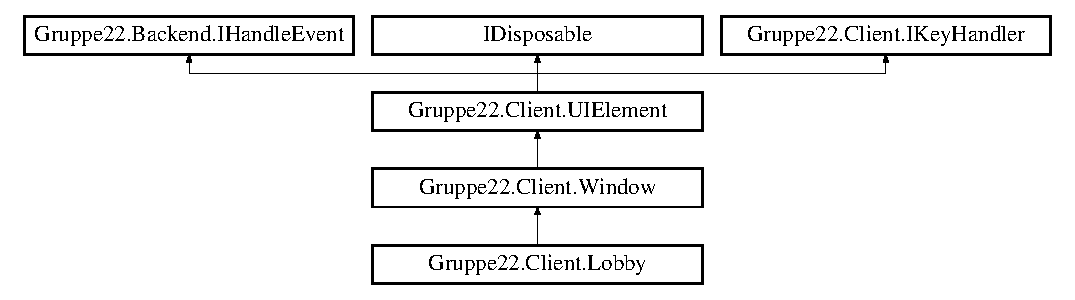
\includegraphics[height=3.589744cm]{class_gruppe22_1_1_client_1_1_lobby}
\end{center}
\end{figure}
\subsection*{Öffentliche Methoden}
\begin{DoxyCompactItemize}
\item 
override void \hyperlink{class_gruppe22_1_1_client_1_1_lobby_ae8c225cc62637fcb8edf68005286fed7}{Update} (Game\-Time game\-Time)
\item 
override void \hyperlink{class_gruppe22_1_1_client_1_1_lobby_a6e3f6336d5da9e230ecf852763c5d605}{Handle\-Event} (bool Down\-Stream, \hyperlink{namespace_gruppe22_1_1_backend_ab56df91bb0bdafa1ea978e552209ce73}{Backend.\-Events} event\-I\-D, params object\mbox{[}$\,$\mbox{]} data)
\item 
\hyperlink{class_gruppe22_1_1_client_1_1_lobby_a6d04a3dc119f01f1a6813a2826c235ad}{Lobby} (\hyperlink{interface_gruppe22_1_1_backend_1_1_i_handle_event}{Backend.\-I\-Handle\-Event} parent, Sprite\-Batch sprite\-Batch, Content\-Manager content, Rectangle display\-Rect)
\end{DoxyCompactItemize}
\subsection*{Weitere Geerbte Elemente}


\subsection{Beschreibung der Konstruktoren und Destruktoren}
\hypertarget{class_gruppe22_1_1_client_1_1_lobby_a6d04a3dc119f01f1a6813a2826c235ad}{\index{Gruppe22\-::\-Client\-::\-Lobby@{Gruppe22\-::\-Client\-::\-Lobby}!Lobby@{Lobby}}
\index{Lobby@{Lobby}!Gruppe22::Client::Lobby@{Gruppe22\-::\-Client\-::\-Lobby}}
\subsubsection[{Lobby}]{\setlength{\rightskip}{0pt plus 5cm}Gruppe22.\-Client.\-Lobby.\-Lobby (
\begin{DoxyParamCaption}
\item[{{\bf Backend.\-I\-Handle\-Event}}]{parent, }
\item[{Sprite\-Batch}]{sprite\-Batch, }
\item[{Content\-Manager}]{content, }
\item[{Rectangle}]{display\-Rect}
\end{DoxyParamCaption}
)}}\label{class_gruppe22_1_1_client_1_1_lobby_a6d04a3dc119f01f1a6813a2826c235ad}


\subsection{Dokumentation der Elementfunktionen}
\hypertarget{class_gruppe22_1_1_client_1_1_lobby_a6e3f6336d5da9e230ecf852763c5d605}{\index{Gruppe22\-::\-Client\-::\-Lobby@{Gruppe22\-::\-Client\-::\-Lobby}!Handle\-Event@{Handle\-Event}}
\index{Handle\-Event@{Handle\-Event}!Gruppe22::Client::Lobby@{Gruppe22\-::\-Client\-::\-Lobby}}
\subsubsection[{Handle\-Event}]{\setlength{\rightskip}{0pt plus 5cm}override void Gruppe22.\-Client.\-Lobby.\-Handle\-Event (
\begin{DoxyParamCaption}
\item[{bool}]{Down\-Stream, }
\item[{{\bf Backend.\-Events}}]{event\-I\-D, }
\item[{params object\mbox{[}$\,$\mbox{]}}]{data}
\end{DoxyParamCaption}
)\hspace{0.3cm}{\ttfamily [virtual]}}}\label{class_gruppe22_1_1_client_1_1_lobby_a6e3f6336d5da9e230ecf852763c5d605}


Erneute Implementation von \hyperlink{class_gruppe22_1_1_client_1_1_u_i_element_ad06a1ce6c1705a1c7aa91756f368a517}{Gruppe22.\-Client.\-U\-I\-Element}.

\hypertarget{class_gruppe22_1_1_client_1_1_lobby_ae8c225cc62637fcb8edf68005286fed7}{\index{Gruppe22\-::\-Client\-::\-Lobby@{Gruppe22\-::\-Client\-::\-Lobby}!Update@{Update}}
\index{Update@{Update}!Gruppe22::Client::Lobby@{Gruppe22\-::\-Client\-::\-Lobby}}
\subsubsection[{Update}]{\setlength{\rightskip}{0pt plus 5cm}override void Gruppe22.\-Client.\-Lobby.\-Update (
\begin{DoxyParamCaption}
\item[{Game\-Time}]{game\-Time}
\end{DoxyParamCaption}
)\hspace{0.3cm}{\ttfamily [virtual]}}}\label{class_gruppe22_1_1_client_1_1_lobby_ae8c225cc62637fcb8edf68005286fed7}





\begin{DoxyParams}{Parameter}
{\em game\-Time} & \\
\hline
\end{DoxyParams}


Erneute Implementation von \hyperlink{class_gruppe22_1_1_client_1_1_u_i_element_a456bc763b6ed6ab441bb0ae96b6f4f8b}{Gruppe22.\-Client.\-U\-I\-Element}.



Die Dokumentation für diese Klasse wurde erzeugt aufgrund der Datei\-:\begin{DoxyCompactItemize}
\item 
C\-:/\-Users/beursken/\-Documents/\-Git\-Hub/gruppe22/\-Gruppe22/\-Gruppe22/\-Client/\-Network/\hyperlink{_lobby_8cs}{Lobby.\-cs}\end{DoxyCompactItemize}

\hypertarget{class_gruppe22_1_1_client_1_1_mainmap}{\section{Gruppe22.\-Client.\-Mainmap Klassenreferenz}
\label{class_gruppe22_1_1_client_1_1_mainmap}\index{Gruppe22.\-Client.\-Mainmap@{Gruppe22.\-Client.\-Mainmap}}
}


The core display of the current part of the dungeon  


Klassendiagramm für Gruppe22.\-Client.\-Mainmap\-:\begin{figure}[H]
\begin{center}
\leavevmode
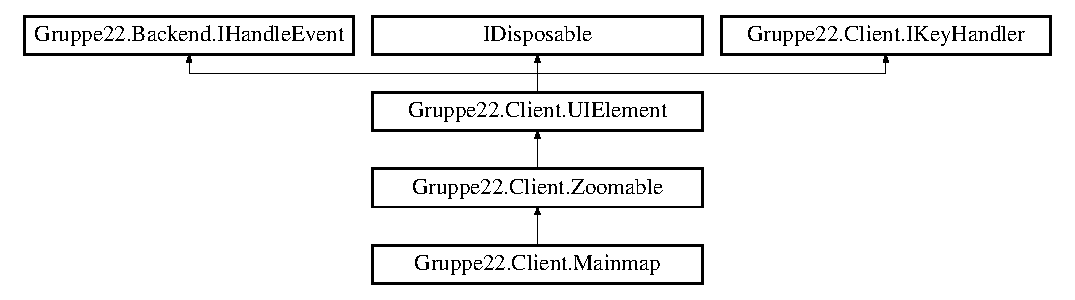
\includegraphics[height=3.589744cm]{class_gruppe22_1_1_client_1_1_mainmap}
\end{center}
\end{figure}
\subsection*{Öffentliche Methoden}
\begin{DoxyCompactItemize}
\item 
void \hyperlink{class_gruppe22_1_1_client_1_1_mainmap_a9936914d9373c75eff572c9b2442a305}{add\-Effect} (int animation\-I\-D, \hyperlink{class_gruppe22_1_1_backend_1_1_coords}{Backend.\-Coords} pos)
\item 
void \hyperlink{class_gruppe22_1_1_client_1_1_mainmap_aca5456f7739a950a12c1c64c829d574d}{Display\-Subtitle} (string main=\char`\"{}\char`\"{}, string sub=\char`\"{}\char`\"{})
\item 
override void \hyperlink{class_gruppe22_1_1_client_1_1_mainmap_adaff683f9444d9fa87c22b51886da78a}{Handle\-Event} (bool Down\-Stream, \hyperlink{namespace_gruppe22_1_1_backend_ab56df91bb0bdafa1ea978e552209ce73}{Backend.\-Events} event\-I\-D, params object\mbox{[}$\,$\mbox{]} data)
\item 
override void \hyperlink{class_gruppe22_1_1_client_1_1_mainmap_a23697dc218e8c4a44feef0f92fa3faf6}{Draw} (Game\-Time gametime)
\begin{DoxyCompactList}\small\item\em Draw the Map \end{DoxyCompactList}\item 
\hyperlink{namespace_gruppe22_1_1_client_aa675883495b38ce0697938ab6300d990}{Wall\-Dir} \hyperlink{class_gruppe22_1_1_client_1_1_mainmap_ac62bde943b1752a7612a8f8030f76088}{Get\-Wall\-Style} (int x=0, int y=0, bool Check\-Wall=true, int Floor\-Style=-\/1)
\begin{DoxyCompactList}\small\item\em Determine wall style to use depending on surrounding squares \end{DoxyCompactList}\item 
bool \hyperlink{class_gruppe22_1_1_client_1_1_mainmap_a93e6f2920cbad8f0add8ac161f17fc7e}{Is\-Moving} (int id)
\item 
void \hyperlink{class_gruppe22_1_1_client_1_1_mainmap_af8ba0ebfcfdb304a2eb3d308839d4a05}{Change\-Dir} (int id, \hyperlink{namespace_gruppe22_1_1_backend_a2d53d5d14b8ea0951ba6971e5da1ebf5}{Backend.\-Direction} dir)
\item 
void \hyperlink{class_gruppe22_1_1_client_1_1_mainmap_a505cd7b8e7a9b55d2e0816b4f52477a3}{reset\-Actors} ()
\item 
void \hyperlink{class_gruppe22_1_1_client_1_1_mainmap_a36fce64e823ffd422e3851c290f0fe87}{float\-Number} (\hyperlink{class_gruppe22_1_1_backend_1_1_coords}{Backend.\-Coords} tile, string text, Color color)
\item 
override void \hyperlink{class_gruppe22_1_1_client_1_1_mainmap_aae564d34ea6375ae7538699c14006e0a}{Update} (Game\-Time game\-Time)
\begin{DoxyCompactList}\small\item\em Move camera, react to mouse \end{DoxyCompactList}\item 
uint \hyperlink{class_gruppe22_1_1_client_1_1_mainmap_a094fdb3d9a640b023d8d5b8141008116}{Add\-Projectile} (\hyperlink{class_gruppe22_1_1_backend_1_1_coords}{Backend.\-Coords} coords, \hyperlink{namespace_gruppe22_1_1_backend_a2d53d5d14b8ea0951ba6971e5da1ebf5}{Backend.\-Direction} dir, \hyperlink{class_gruppe22_1_1_projectile_tile}{Projectile\-Tile} tile)
\item 
void \hyperlink{class_gruppe22_1_1_client_1_1_mainmap_a89080aef56b9428f2a0fab05a675eb07}{Remove\-Projectile} (uint id)
\item 
\hyperlink{class_gruppe22_1_1_client_1_1_projectile}{Projectile} \hyperlink{class_gruppe22_1_1_client_1_1_mainmap_a71ee6cf7e84b63a5f334ba7eedf55476}{Get\-Projectile} (uint id)
\item 
void \hyperlink{class_gruppe22_1_1_client_1_1_mainmap_a744dd8cd83091b23cf44b968937f513c}{Fire\-Projectile} ()
\item 
override void \hyperlink{class_gruppe22_1_1_client_1_1_mainmap_a5aacac737e9a500f6c2b5492ce1a9f71}{Move\-Content} (Vector2 difference, int \-\_\-last\-Check=0)
\begin{DoxyCompactList}\small\item\em Disable moving map by mouse drag to avoid conflicts with move by click \end{DoxyCompactList}\item 
void \hyperlink{class_gruppe22_1_1_client_1_1_mainmap_aa05339d33c57fa642006a430f6ab35f7}{Move\-Player} (\hyperlink{namespace_gruppe22_1_1_backend_a2d53d5d14b8ea0951ba6971e5da1ebf5}{Backend.\-Direction} dir)
\begin{DoxyCompactList}\small\item\em Check whether player can move to a certain square from current position \end{DoxyCompactList}\item 
\hyperlink{class_gruppe22_1_1_client_1_1_mainmap_a9740c0af18e7fb685f0bab990f082ac2}{Mainmap} (\hyperlink{interface_gruppe22_1_1_backend_1_1_i_handle_event}{Backend.\-I\-Handle\-Event} parent, Sprite\-Batch sprite\-Batch, Content\-Manager content, Rectangle display\-Area, \hyperlink{class_gruppe22_1_1_backend_1_1_map}{Backend.\-Map} map, bool \hyperlink{class_gruppe22_1_1_client_1_1_mainmap_a05d1ac6585e8e336a812443bfead1617}{enabled}=true)
\begin{DoxyCompactList}\small\item\em Create the visible version of the game map \end{DoxyCompactList}\end{DoxyCompactItemize}
\subsection*{Öffentliche, statische Methoden}
\begin{DoxyCompactItemize}
\item 
static Rectangle \hyperlink{class_gruppe22_1_1_client_1_1_mainmap_a4bb4a6696e30f92aa794948ec5bbac40}{\-\_\-tile\-Rect} (Vector2 coords, bool tall=false)
\item 
static \hyperlink{class_gruppe22_1_1_backend_1_1_coords}{Backend.\-Coords} \hyperlink{class_gruppe22_1_1_client_1_1_mainmap_a4284eda383663111f1ae9d35e32ddf36}{\-\_\-map2screen} (\hyperlink{class_gruppe22_1_1_backend_1_1_coords}{Backend.\-Coords} map\-C, bool tall=false)
\item 
static \hyperlink{class_gruppe22_1_1_backend_1_1_coords}{Backend.\-Coords} \hyperlink{class_gruppe22_1_1_client_1_1_mainmap_a3550c63a5b95bd95b2b8cc558ada4652}{\-\_\-map2screen} (int x, int y, bool tall=false)
\item 
static \hyperlink{class_gruppe22_1_1_backend_1_1_coords}{Backend.\-Coords} \hyperlink{class_gruppe22_1_1_client_1_1_mainmap_a8030ba7ebffc39ced0ca61ad6e8a5ff1}{\-\_\-screen2map} (\hyperlink{class_gruppe22_1_1_backend_1_1_coords}{Backend.\-Coords} screen\-C, bool tall=false)
\begin{DoxyCompactList}\small\item\em Determine tile based on coordinates of point \end{DoxyCompactList}\item 
static \hyperlink{class_gruppe22_1_1_backend_1_1_coords}{Backend.\-Coords} \hyperlink{class_gruppe22_1_1_client_1_1_mainmap_a709f8e5e62d8f603bdfc0f447b20982f}{\-\_\-screen2map} (int x, int y, bool tall=false)
\begin{DoxyCompactList}\small\item\em Determine tile based on coordinates of point \end{DoxyCompactList}\item 
static \hyperlink{class_gruppe22_1_1_backend_1_1_coords}{Backend.\-Coords} \hyperlink{class_gruppe22_1_1_client_1_1_mainmap_a4143327f197fcbda55723d6a7bb8dcfb}{\-\_\-pos2\-Tile} (Vector2 coords, bool tall=false)
\begin{DoxyCompactList}\small\item\em Determine tile based on coordinates of point \end{DoxyCompactList}\end{DoxyCompactItemize}
\subsection*{Propertys}
\begin{DoxyCompactItemize}
\item 
List$<$ \hyperlink{class_gruppe22_1_1_client_1_1_actor_view}{Actor\-View} $>$ \hyperlink{class_gruppe22_1_1_client_1_1_mainmap_a3052907545bdede0789a79cc25b15883}{actors}\hspace{0.3cm}{\ttfamily  \mbox{[}get\mbox{]}}
\item 
Matrix \hyperlink{class_gruppe22_1_1_client_1_1_mainmap_a1fcf58729b476ec0b4e3ccb8bb2ba642}{transform\-Matrix}\hspace{0.3cm}{\ttfamily  \mbox{[}get\mbox{]}}
\item 
bool \hyperlink{class_gruppe22_1_1_client_1_1_mainmap_a05d1ac6585e8e336a812443bfead1617}{enabled}\hspace{0.3cm}{\ttfamily  \mbox{[}get, set\mbox{]}}
\item 
bool \hyperlink{class_gruppe22_1_1_client_1_1_mainmap_ad868efaa137848bf9692b8b51b763a6c}{no\-Move}\hspace{0.3cm}{\ttfamily  \mbox{[}get, set\mbox{]}}
\end{DoxyCompactItemize}
\subsection*{Weitere Geerbte Elemente}


\subsection{Ausführliche Beschreibung}
The core display of the current part of the dungeon 



\subsection{Beschreibung der Konstruktoren und Destruktoren}
\hypertarget{class_gruppe22_1_1_client_1_1_mainmap_a9740c0af18e7fb685f0bab990f082ac2}{\index{Gruppe22\-::\-Client\-::\-Mainmap@{Gruppe22\-::\-Client\-::\-Mainmap}!Mainmap@{Mainmap}}
\index{Mainmap@{Mainmap}!Gruppe22::Client::Mainmap@{Gruppe22\-::\-Client\-::\-Mainmap}}
\subsubsection[{Mainmap}]{\setlength{\rightskip}{0pt plus 5cm}Gruppe22.\-Client.\-Mainmap.\-Mainmap (
\begin{DoxyParamCaption}
\item[{{\bf Backend.\-I\-Handle\-Event}}]{parent, }
\item[{Sprite\-Batch}]{sprite\-Batch, }
\item[{Content\-Manager}]{content, }
\item[{Rectangle}]{display\-Area, }
\item[{{\bf Backend.\-Map}}]{map, }
\item[{bool}]{enabled = {\ttfamily true}}
\end{DoxyParamCaption}
)}}\label{class_gruppe22_1_1_client_1_1_mainmap_a9740c0af18e7fb685f0bab990f082ac2}


Create the visible version of the game map 


\begin{DoxyParams}{Parameter}
{\em graphics} & The core graphics device manager\\
\hline
{\em sprite\-Batch} & A sprite batch used for drawing\\
\hline
{\em display\-Area} & The area on wich the map will be placed\\
\hline
{\em floor} & The textures used for the floor\\
\hline
{\em wall1} & A set of tiles for the walls\\
\hline
{\em wall2} & A set of tiles for doors\\
\hline
{\em map} & Internal storage of map data\\
\hline
\end{DoxyParams}


\subsection{Dokumentation der Elementfunktionen}
\hypertarget{class_gruppe22_1_1_client_1_1_mainmap_a4284eda383663111f1ae9d35e32ddf36}{\index{Gruppe22\-::\-Client\-::\-Mainmap@{Gruppe22\-::\-Client\-::\-Mainmap}!\-\_\-map2screen@{\-\_\-map2screen}}
\index{\-\_\-map2screen@{\-\_\-map2screen}!Gruppe22::Client::Mainmap@{Gruppe22\-::\-Client\-::\-Mainmap}}
\subsubsection[{\-\_\-map2screen}]{\setlength{\rightskip}{0pt plus 5cm}static {\bf Backend.\-Coords} Gruppe22.\-Client.\-Mainmap.\-\_\-map2screen (
\begin{DoxyParamCaption}
\item[{{\bf Backend.\-Coords}}]{map\-C, }
\item[{bool}]{tall = {\ttfamily false}}
\end{DoxyParamCaption}
)\hspace{0.3cm}{\ttfamily [static]}}}\label{class_gruppe22_1_1_client_1_1_mainmap_a4284eda383663111f1ae9d35e32ddf36}





\begin{DoxyParams}{Parameter}
{\em coords} & \\
\hline
{\em tall} & \\
\hline
\end{DoxyParams}
\begin{DoxyReturn}{Rückgabe}

\end{DoxyReturn}
\hypertarget{class_gruppe22_1_1_client_1_1_mainmap_a3550c63a5b95bd95b2b8cc558ada4652}{\index{Gruppe22\-::\-Client\-::\-Mainmap@{Gruppe22\-::\-Client\-::\-Mainmap}!\-\_\-map2screen@{\-\_\-map2screen}}
\index{\-\_\-map2screen@{\-\_\-map2screen}!Gruppe22::Client::Mainmap@{Gruppe22\-::\-Client\-::\-Mainmap}}
\subsubsection[{\-\_\-map2screen}]{\setlength{\rightskip}{0pt plus 5cm}static {\bf Backend.\-Coords} Gruppe22.\-Client.\-Mainmap.\-\_\-map2screen (
\begin{DoxyParamCaption}
\item[{int}]{x, }
\item[{int}]{y, }
\item[{bool}]{tall = {\ttfamily false}}
\end{DoxyParamCaption}
)\hspace{0.3cm}{\ttfamily [static]}}}\label{class_gruppe22_1_1_client_1_1_mainmap_a3550c63a5b95bd95b2b8cc558ada4652}





\begin{DoxyParams}{Parameter}
{\em coords} & \\
\hline
{\em tall} & \\
\hline
\end{DoxyParams}
\begin{DoxyReturn}{Rückgabe}

\end{DoxyReturn}
\hypertarget{class_gruppe22_1_1_client_1_1_mainmap_a4143327f197fcbda55723d6a7bb8dcfb}{\index{Gruppe22\-::\-Client\-::\-Mainmap@{Gruppe22\-::\-Client\-::\-Mainmap}!\-\_\-pos2\-Tile@{\-\_\-pos2\-Tile}}
\index{\-\_\-pos2\-Tile@{\-\_\-pos2\-Tile}!Gruppe22::Client::Mainmap@{Gruppe22\-::\-Client\-::\-Mainmap}}
\subsubsection[{\-\_\-pos2\-Tile}]{\setlength{\rightskip}{0pt plus 5cm}static {\bf Backend.\-Coords} Gruppe22.\-Client.\-Mainmap.\-\_\-pos2\-Tile (
\begin{DoxyParamCaption}
\item[{Vector2}]{coords, }
\item[{bool}]{tall = {\ttfamily false}}
\end{DoxyParamCaption}
)\hspace{0.3cm}{\ttfamily [static]}}}\label{class_gruppe22_1_1_client_1_1_mainmap_a4143327f197fcbda55723d6a7bb8dcfb}


Determine tile based on coordinates of point 


\begin{DoxyParams}{Parameter}
{\em coords} & \\
\hline
{\em tall} & \\
\hline
\end{DoxyParams}
\begin{DoxyReturn}{Rückgabe}

\end{DoxyReturn}
\hypertarget{class_gruppe22_1_1_client_1_1_mainmap_a8030ba7ebffc39ced0ca61ad6e8a5ff1}{\index{Gruppe22\-::\-Client\-::\-Mainmap@{Gruppe22\-::\-Client\-::\-Mainmap}!\-\_\-screen2map@{\-\_\-screen2map}}
\index{\-\_\-screen2map@{\-\_\-screen2map}!Gruppe22::Client::Mainmap@{Gruppe22\-::\-Client\-::\-Mainmap}}
\subsubsection[{\-\_\-screen2map}]{\setlength{\rightskip}{0pt plus 5cm}static {\bf Backend.\-Coords} Gruppe22.\-Client.\-Mainmap.\-\_\-screen2map (
\begin{DoxyParamCaption}
\item[{{\bf Backend.\-Coords}}]{screen\-C, }
\item[{bool}]{tall = {\ttfamily false}}
\end{DoxyParamCaption}
)\hspace{0.3cm}{\ttfamily [static]}}}\label{class_gruppe22_1_1_client_1_1_mainmap_a8030ba7ebffc39ced0ca61ad6e8a5ff1}


Determine tile based on coordinates of point 


\begin{DoxyParams}{Parameter}
{\em coords} & \\
\hline
{\em tall} & \\
\hline
\end{DoxyParams}
\begin{DoxyReturn}{Rückgabe}

\end{DoxyReturn}
\hypertarget{class_gruppe22_1_1_client_1_1_mainmap_a709f8e5e62d8f603bdfc0f447b20982f}{\index{Gruppe22\-::\-Client\-::\-Mainmap@{Gruppe22\-::\-Client\-::\-Mainmap}!\-\_\-screen2map@{\-\_\-screen2map}}
\index{\-\_\-screen2map@{\-\_\-screen2map}!Gruppe22::Client::Mainmap@{Gruppe22\-::\-Client\-::\-Mainmap}}
\subsubsection[{\-\_\-screen2map}]{\setlength{\rightskip}{0pt plus 5cm}static {\bf Backend.\-Coords} Gruppe22.\-Client.\-Mainmap.\-\_\-screen2map (
\begin{DoxyParamCaption}
\item[{int}]{x, }
\item[{int}]{y, }
\item[{bool}]{tall = {\ttfamily false}}
\end{DoxyParamCaption}
)\hspace{0.3cm}{\ttfamily [static]}}}\label{class_gruppe22_1_1_client_1_1_mainmap_a709f8e5e62d8f603bdfc0f447b20982f}


Determine tile based on coordinates of point 


\begin{DoxyParams}{Parameter}
{\em coords} & \\
\hline
{\em tall} & \\
\hline
\end{DoxyParams}
\begin{DoxyReturn}{Rückgabe}

\end{DoxyReturn}
\hypertarget{class_gruppe22_1_1_client_1_1_mainmap_a4bb4a6696e30f92aa794948ec5bbac40}{\index{Gruppe22\-::\-Client\-::\-Mainmap@{Gruppe22\-::\-Client\-::\-Mainmap}!\-\_\-tile\-Rect@{\-\_\-tile\-Rect}}
\index{\-\_\-tile\-Rect@{\-\_\-tile\-Rect}!Gruppe22::Client::Mainmap@{Gruppe22\-::\-Client\-::\-Mainmap}}
\subsubsection[{\-\_\-tile\-Rect}]{\setlength{\rightskip}{0pt plus 5cm}static Rectangle Gruppe22.\-Client.\-Mainmap.\-\_\-tile\-Rect (
\begin{DoxyParamCaption}
\item[{Vector2}]{coords, }
\item[{bool}]{tall = {\ttfamily false}}
\end{DoxyParamCaption}
)\hspace{0.3cm}{\ttfamily [static]}}}\label{class_gruppe22_1_1_client_1_1_mainmap_a4bb4a6696e30f92aa794948ec5bbac40}





\begin{DoxyParams}{Parameter}
{\em coords} & \\
\hline
{\em tall} & \\
\hline
\end{DoxyParams}
\begin{DoxyReturn}{Rückgabe}

\end{DoxyReturn}
\hypertarget{class_gruppe22_1_1_client_1_1_mainmap_a9936914d9373c75eff572c9b2442a305}{\index{Gruppe22\-::\-Client\-::\-Mainmap@{Gruppe22\-::\-Client\-::\-Mainmap}!add\-Effect@{add\-Effect}}
\index{add\-Effect@{add\-Effect}!Gruppe22::Client::Mainmap@{Gruppe22\-::\-Client\-::\-Mainmap}}
\subsubsection[{add\-Effect}]{\setlength{\rightskip}{0pt plus 5cm}void Gruppe22.\-Client.\-Mainmap.\-add\-Effect (
\begin{DoxyParamCaption}
\item[{int}]{animation\-I\-D, }
\item[{{\bf Backend.\-Coords}}]{pos}
\end{DoxyParamCaption}
)}}\label{class_gruppe22_1_1_client_1_1_mainmap_a9936914d9373c75eff572c9b2442a305}
\hypertarget{class_gruppe22_1_1_client_1_1_mainmap_a094fdb3d9a640b023d8d5b8141008116}{\index{Gruppe22\-::\-Client\-::\-Mainmap@{Gruppe22\-::\-Client\-::\-Mainmap}!Add\-Projectile@{Add\-Projectile}}
\index{Add\-Projectile@{Add\-Projectile}!Gruppe22::Client::Mainmap@{Gruppe22\-::\-Client\-::\-Mainmap}}
\subsubsection[{Add\-Projectile}]{\setlength{\rightskip}{0pt plus 5cm}uint Gruppe22.\-Client.\-Mainmap.\-Add\-Projectile (
\begin{DoxyParamCaption}
\item[{{\bf Backend.\-Coords}}]{coords, }
\item[{{\bf Backend.\-Direction}}]{dir, }
\item[{{\bf Projectile\-Tile}}]{tile}
\end{DoxyParamCaption}
)}}\label{class_gruppe22_1_1_client_1_1_mainmap_a094fdb3d9a640b023d8d5b8141008116}
\hypertarget{class_gruppe22_1_1_client_1_1_mainmap_af8ba0ebfcfdb304a2eb3d308839d4a05}{\index{Gruppe22\-::\-Client\-::\-Mainmap@{Gruppe22\-::\-Client\-::\-Mainmap}!Change\-Dir@{Change\-Dir}}
\index{Change\-Dir@{Change\-Dir}!Gruppe22::Client::Mainmap@{Gruppe22\-::\-Client\-::\-Mainmap}}
\subsubsection[{Change\-Dir}]{\setlength{\rightskip}{0pt plus 5cm}void Gruppe22.\-Client.\-Mainmap.\-Change\-Dir (
\begin{DoxyParamCaption}
\item[{int}]{id, }
\item[{{\bf Backend.\-Direction}}]{dir}
\end{DoxyParamCaption}
)}}\label{class_gruppe22_1_1_client_1_1_mainmap_af8ba0ebfcfdb304a2eb3d308839d4a05}
\hypertarget{class_gruppe22_1_1_client_1_1_mainmap_aca5456f7739a950a12c1c64c829d574d}{\index{Gruppe22\-::\-Client\-::\-Mainmap@{Gruppe22\-::\-Client\-::\-Mainmap}!Display\-Subtitle@{Display\-Subtitle}}
\index{Display\-Subtitle@{Display\-Subtitle}!Gruppe22::Client::Mainmap@{Gruppe22\-::\-Client\-::\-Mainmap}}
\subsubsection[{Display\-Subtitle}]{\setlength{\rightskip}{0pt plus 5cm}void Gruppe22.\-Client.\-Mainmap.\-Display\-Subtitle (
\begin{DoxyParamCaption}
\item[{string}]{main = {\ttfamily \char`\"{}\char`\"{}}, }
\item[{string}]{sub = {\ttfamily \char`\"{}\char`\"{}}}
\end{DoxyParamCaption}
)}}\label{class_gruppe22_1_1_client_1_1_mainmap_aca5456f7739a950a12c1c64c829d574d}
\hypertarget{class_gruppe22_1_1_client_1_1_mainmap_a23697dc218e8c4a44feef0f92fa3faf6}{\index{Gruppe22\-::\-Client\-::\-Mainmap@{Gruppe22\-::\-Client\-::\-Mainmap}!Draw@{Draw}}
\index{Draw@{Draw}!Gruppe22::Client::Mainmap@{Gruppe22\-::\-Client\-::\-Mainmap}}
\subsubsection[{Draw}]{\setlength{\rightskip}{0pt plus 5cm}override void Gruppe22.\-Client.\-Mainmap.\-Draw (
\begin{DoxyParamCaption}
\item[{Game\-Time}]{gametime}
\end{DoxyParamCaption}
)\hspace{0.3cm}{\ttfamily [virtual]}}}\label{class_gruppe22_1_1_client_1_1_mainmap_a23697dc218e8c4a44feef0f92fa3faf6}


Draw the Map 



Erneute Implementation von \hyperlink{class_gruppe22_1_1_client_1_1_u_i_element_ae68afcbd1db3540052d6b399022e56e7}{Gruppe22.\-Client.\-U\-I\-Element}.

\hypertarget{class_gruppe22_1_1_client_1_1_mainmap_a744dd8cd83091b23cf44b968937f513c}{\index{Gruppe22\-::\-Client\-::\-Mainmap@{Gruppe22\-::\-Client\-::\-Mainmap}!Fire\-Projectile@{Fire\-Projectile}}
\index{Fire\-Projectile@{Fire\-Projectile}!Gruppe22::Client::Mainmap@{Gruppe22\-::\-Client\-::\-Mainmap}}
\subsubsection[{Fire\-Projectile}]{\setlength{\rightskip}{0pt plus 5cm}void Gruppe22.\-Client.\-Mainmap.\-Fire\-Projectile (
\begin{DoxyParamCaption}
{}
\end{DoxyParamCaption}
)}}\label{class_gruppe22_1_1_client_1_1_mainmap_a744dd8cd83091b23cf44b968937f513c}
\hypertarget{class_gruppe22_1_1_client_1_1_mainmap_a36fce64e823ffd422e3851c290f0fe87}{\index{Gruppe22\-::\-Client\-::\-Mainmap@{Gruppe22\-::\-Client\-::\-Mainmap}!float\-Number@{float\-Number}}
\index{float\-Number@{float\-Number}!Gruppe22::Client::Mainmap@{Gruppe22\-::\-Client\-::\-Mainmap}}
\subsubsection[{float\-Number}]{\setlength{\rightskip}{0pt plus 5cm}void Gruppe22.\-Client.\-Mainmap.\-float\-Number (
\begin{DoxyParamCaption}
\item[{{\bf Backend.\-Coords}}]{tile, }
\item[{string}]{text, }
\item[{Color}]{color}
\end{DoxyParamCaption}
)}}\label{class_gruppe22_1_1_client_1_1_mainmap_a36fce64e823ffd422e3851c290f0fe87}
\hypertarget{class_gruppe22_1_1_client_1_1_mainmap_a71ee6cf7e84b63a5f334ba7eedf55476}{\index{Gruppe22\-::\-Client\-::\-Mainmap@{Gruppe22\-::\-Client\-::\-Mainmap}!Get\-Projectile@{Get\-Projectile}}
\index{Get\-Projectile@{Get\-Projectile}!Gruppe22::Client::Mainmap@{Gruppe22\-::\-Client\-::\-Mainmap}}
\subsubsection[{Get\-Projectile}]{\setlength{\rightskip}{0pt plus 5cm}{\bf Projectile} Gruppe22.\-Client.\-Mainmap.\-Get\-Projectile (
\begin{DoxyParamCaption}
\item[{uint}]{id}
\end{DoxyParamCaption}
)}}\label{class_gruppe22_1_1_client_1_1_mainmap_a71ee6cf7e84b63a5f334ba7eedf55476}
\hypertarget{class_gruppe22_1_1_client_1_1_mainmap_ac62bde943b1752a7612a8f8030f76088}{\index{Gruppe22\-::\-Client\-::\-Mainmap@{Gruppe22\-::\-Client\-::\-Mainmap}!Get\-Wall\-Style@{Get\-Wall\-Style}}
\index{Get\-Wall\-Style@{Get\-Wall\-Style}!Gruppe22::Client::Mainmap@{Gruppe22\-::\-Client\-::\-Mainmap}}
\subsubsection[{Get\-Wall\-Style}]{\setlength{\rightskip}{0pt plus 5cm}{\bf Wall\-Dir} Gruppe22.\-Client.\-Mainmap.\-Get\-Wall\-Style (
\begin{DoxyParamCaption}
\item[{int}]{x = {\ttfamily 0}, }
\item[{int}]{y = {\ttfamily 0}, }
\item[{bool}]{Check\-Wall = {\ttfamily true}, }
\item[{int}]{Floor\-Style = {\ttfamily -\/1}}
\end{DoxyParamCaption}
)}}\label{class_gruppe22_1_1_client_1_1_mainmap_ac62bde943b1752a7612a8f8030f76088}


Determine wall style to use depending on surrounding squares 


\begin{DoxyParams}{Parameter}
{\em x} & horizontal coordinate of square to check\\
\hline
{\em y} & vertical coordinate of square to check\\
\hline
\end{DoxyParams}
\begin{DoxyReturn}{Rückgabe}
A direction to be used for the wall
\end{DoxyReturn}
\hypertarget{class_gruppe22_1_1_client_1_1_mainmap_adaff683f9444d9fa87c22b51886da78a}{\index{Gruppe22\-::\-Client\-::\-Mainmap@{Gruppe22\-::\-Client\-::\-Mainmap}!Handle\-Event@{Handle\-Event}}
\index{Handle\-Event@{Handle\-Event}!Gruppe22::Client::Mainmap@{Gruppe22\-::\-Client\-::\-Mainmap}}
\subsubsection[{Handle\-Event}]{\setlength{\rightskip}{0pt plus 5cm}override void Gruppe22.\-Client.\-Mainmap.\-Handle\-Event (
\begin{DoxyParamCaption}
\item[{bool}]{Down\-Stream, }
\item[{{\bf Backend.\-Events}}]{event\-I\-D, }
\item[{params object\mbox{[}$\,$\mbox{]}}]{data}
\end{DoxyParamCaption}
)\hspace{0.3cm}{\ttfamily [virtual]}}}\label{class_gruppe22_1_1_client_1_1_mainmap_adaff683f9444d9fa87c22b51886da78a}


Erneute Implementation von \hyperlink{class_gruppe22_1_1_client_1_1_u_i_element_ad06a1ce6c1705a1c7aa91756f368a517}{Gruppe22.\-Client.\-U\-I\-Element}.

\hypertarget{class_gruppe22_1_1_client_1_1_mainmap_a93e6f2920cbad8f0add8ac161f17fc7e}{\index{Gruppe22\-::\-Client\-::\-Mainmap@{Gruppe22\-::\-Client\-::\-Mainmap}!Is\-Moving@{Is\-Moving}}
\index{Is\-Moving@{Is\-Moving}!Gruppe22::Client::Mainmap@{Gruppe22\-::\-Client\-::\-Mainmap}}
\subsubsection[{Is\-Moving}]{\setlength{\rightskip}{0pt plus 5cm}bool Gruppe22.\-Client.\-Mainmap.\-Is\-Moving (
\begin{DoxyParamCaption}
\item[{int}]{id}
\end{DoxyParamCaption}
)}}\label{class_gruppe22_1_1_client_1_1_mainmap_a93e6f2920cbad8f0add8ac161f17fc7e}
\hypertarget{class_gruppe22_1_1_client_1_1_mainmap_a5aacac737e9a500f6c2b5492ce1a9f71}{\index{Gruppe22\-::\-Client\-::\-Mainmap@{Gruppe22\-::\-Client\-::\-Mainmap}!Move\-Content@{Move\-Content}}
\index{Move\-Content@{Move\-Content}!Gruppe22::Client::Mainmap@{Gruppe22\-::\-Client\-::\-Mainmap}}
\subsubsection[{Move\-Content}]{\setlength{\rightskip}{0pt plus 5cm}override void Gruppe22.\-Client.\-Mainmap.\-Move\-Content (
\begin{DoxyParamCaption}
\item[{Vector2}]{difference, }
\item[{int}]{\-\_\-last\-Check = {\ttfamily 0}}
\end{DoxyParamCaption}
)\hspace{0.3cm}{\ttfamily [virtual]}}}\label{class_gruppe22_1_1_client_1_1_mainmap_a5aacac737e9a500f6c2b5492ce1a9f71}


Disable moving map by mouse drag to avoid conflicts with move by click 


\begin{DoxyParams}{Parameter}
{\em difference} & \\
\hline
{\em \-\_\-last\-Check} & \\
\hline
\end{DoxyParams}


Erneute Implementation von \hyperlink{class_gruppe22_1_1_client_1_1_u_i_element_aa089eaf82ae3a89724a45eb8860cb97b}{Gruppe22.\-Client.\-U\-I\-Element}.

\hypertarget{class_gruppe22_1_1_client_1_1_mainmap_aa05339d33c57fa642006a430f6ab35f7}{\index{Gruppe22\-::\-Client\-::\-Mainmap@{Gruppe22\-::\-Client\-::\-Mainmap}!Move\-Player@{Move\-Player}}
\index{Move\-Player@{Move\-Player}!Gruppe22::Client::Mainmap@{Gruppe22\-::\-Client\-::\-Mainmap}}
\subsubsection[{Move\-Player}]{\setlength{\rightskip}{0pt plus 5cm}void Gruppe22.\-Client.\-Mainmap.\-Move\-Player (
\begin{DoxyParamCaption}
\item[{{\bf Backend.\-Direction}}]{dir}
\end{DoxyParamCaption}
)}}\label{class_gruppe22_1_1_client_1_1_mainmap_aa05339d33c57fa642006a430f6ab35f7}


Check whether player can move to a certain square from current position 


\begin{DoxyParams}{Parameter}
{\em dir} & Direction to move to\\
\hline
\end{DoxyParams}
\hypertarget{class_gruppe22_1_1_client_1_1_mainmap_a89080aef56b9428f2a0fab05a675eb07}{\index{Gruppe22\-::\-Client\-::\-Mainmap@{Gruppe22\-::\-Client\-::\-Mainmap}!Remove\-Projectile@{Remove\-Projectile}}
\index{Remove\-Projectile@{Remove\-Projectile}!Gruppe22::Client::Mainmap@{Gruppe22\-::\-Client\-::\-Mainmap}}
\subsubsection[{Remove\-Projectile}]{\setlength{\rightskip}{0pt plus 5cm}void Gruppe22.\-Client.\-Mainmap.\-Remove\-Projectile (
\begin{DoxyParamCaption}
\item[{uint}]{id}
\end{DoxyParamCaption}
)}}\label{class_gruppe22_1_1_client_1_1_mainmap_a89080aef56b9428f2a0fab05a675eb07}
\hypertarget{class_gruppe22_1_1_client_1_1_mainmap_a505cd7b8e7a9b55d2e0816b4f52477a3}{\index{Gruppe22\-::\-Client\-::\-Mainmap@{Gruppe22\-::\-Client\-::\-Mainmap}!reset\-Actors@{reset\-Actors}}
\index{reset\-Actors@{reset\-Actors}!Gruppe22::Client::Mainmap@{Gruppe22\-::\-Client\-::\-Mainmap}}
\subsubsection[{reset\-Actors}]{\setlength{\rightskip}{0pt plus 5cm}void Gruppe22.\-Client.\-Mainmap.\-reset\-Actors (
\begin{DoxyParamCaption}
{}
\end{DoxyParamCaption}
)}}\label{class_gruppe22_1_1_client_1_1_mainmap_a505cd7b8e7a9b55d2e0816b4f52477a3}
\hypertarget{class_gruppe22_1_1_client_1_1_mainmap_aae564d34ea6375ae7538699c14006e0a}{\index{Gruppe22\-::\-Client\-::\-Mainmap@{Gruppe22\-::\-Client\-::\-Mainmap}!Update@{Update}}
\index{Update@{Update}!Gruppe22::Client::Mainmap@{Gruppe22\-::\-Client\-::\-Mainmap}}
\subsubsection[{Update}]{\setlength{\rightskip}{0pt plus 5cm}override void Gruppe22.\-Client.\-Mainmap.\-Update (
\begin{DoxyParamCaption}
\item[{Game\-Time}]{game\-Time}
\end{DoxyParamCaption}
)\hspace{0.3cm}{\ttfamily [virtual]}}}\label{class_gruppe22_1_1_client_1_1_mainmap_aae564d34ea6375ae7538699c14006e0a}


Move camera, react to mouse 


\begin{DoxyParams}{Parameter}
{\em game\-Time} & \\
\hline
\end{DoxyParams}


Erneute Implementation von \hyperlink{class_gruppe22_1_1_client_1_1_u_i_element_a456bc763b6ed6ab441bb0ae96b6f4f8b}{Gruppe22.\-Client.\-U\-I\-Element}.



\subsection{Dokumentation der Propertys}
\hypertarget{class_gruppe22_1_1_client_1_1_mainmap_a3052907545bdede0789a79cc25b15883}{\index{Gruppe22\-::\-Client\-::\-Mainmap@{Gruppe22\-::\-Client\-::\-Mainmap}!actors@{actors}}
\index{actors@{actors}!Gruppe22::Client::Mainmap@{Gruppe22\-::\-Client\-::\-Mainmap}}
\subsubsection[{actors}]{\setlength{\rightskip}{0pt plus 5cm}List$<${\bf Actor\-View}$>$ Gruppe22.\-Client.\-Mainmap.\-actors\hspace{0.3cm}{\ttfamily [get]}}}\label{class_gruppe22_1_1_client_1_1_mainmap_a3052907545bdede0789a79cc25b15883}
\hypertarget{class_gruppe22_1_1_client_1_1_mainmap_a05d1ac6585e8e336a812443bfead1617}{\index{Gruppe22\-::\-Client\-::\-Mainmap@{Gruppe22\-::\-Client\-::\-Mainmap}!enabled@{enabled}}
\index{enabled@{enabled}!Gruppe22::Client::Mainmap@{Gruppe22\-::\-Client\-::\-Mainmap}}
\subsubsection[{enabled}]{\setlength{\rightskip}{0pt plus 5cm}bool Gruppe22.\-Client.\-Mainmap.\-enabled\hspace{0.3cm}{\ttfamily [get]}, {\ttfamily [set]}}}\label{class_gruppe22_1_1_client_1_1_mainmap_a05d1ac6585e8e336a812443bfead1617}
\hypertarget{class_gruppe22_1_1_client_1_1_mainmap_ad868efaa137848bf9692b8b51b763a6c}{\index{Gruppe22\-::\-Client\-::\-Mainmap@{Gruppe22\-::\-Client\-::\-Mainmap}!no\-Move@{no\-Move}}
\index{no\-Move@{no\-Move}!Gruppe22::Client::Mainmap@{Gruppe22\-::\-Client\-::\-Mainmap}}
\subsubsection[{no\-Move}]{\setlength{\rightskip}{0pt plus 5cm}bool Gruppe22.\-Client.\-Mainmap.\-no\-Move\hspace{0.3cm}{\ttfamily [get]}, {\ttfamily [set]}}}\label{class_gruppe22_1_1_client_1_1_mainmap_ad868efaa137848bf9692b8b51b763a6c}
\hypertarget{class_gruppe22_1_1_client_1_1_mainmap_a1fcf58729b476ec0b4e3ccb8bb2ba642}{\index{Gruppe22\-::\-Client\-::\-Mainmap@{Gruppe22\-::\-Client\-::\-Mainmap}!transform\-Matrix@{transform\-Matrix}}
\index{transform\-Matrix@{transform\-Matrix}!Gruppe22::Client::Mainmap@{Gruppe22\-::\-Client\-::\-Mainmap}}
\subsubsection[{transform\-Matrix}]{\setlength{\rightskip}{0pt plus 5cm}Matrix Gruppe22.\-Client.\-Mainmap.\-transform\-Matrix\hspace{0.3cm}{\ttfamily [get]}}}\label{class_gruppe22_1_1_client_1_1_mainmap_a1fcf58729b476ec0b4e3ccb8bb2ba642}


Die Dokumentation für diese Klasse wurde erzeugt aufgrund der Datei\-:\begin{DoxyCompactItemize}
\item 
C\-:/\-Users/beursken/\-Documents/\-Git\-Hub/gruppe22/\-Gruppe22/\-Gruppe22/\-Client/\-Map/\hyperlink{_mainmap_8cs}{Mainmap.\-cs}\end{DoxyCompactItemize}

\hypertarget{class_gruppe22_1_1_main_window}{\section{Gruppe22.\-Main\-Window Klassenreferenz}
\label{class_gruppe22_1_1_main_window}\index{Gruppe22.\-Main\-Window@{Gruppe22.\-Main\-Window}}
}


The main class (disposing events, handling game logic, reacting to user input)  


Klassendiagramm für Gruppe22.\-Main\-Window\-:\begin{figure}[H]
\begin{center}
\leavevmode
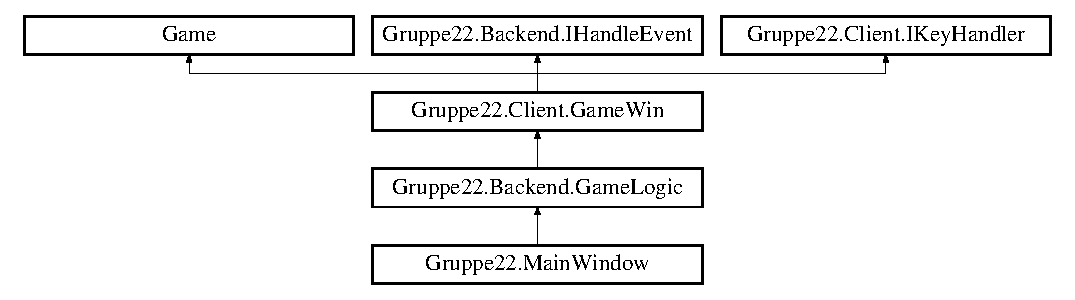
\includegraphics[height=3.589744cm]{class_gruppe22_1_1_main_window}
\end{center}
\end{figure}
\subsection*{Öffentliche Methoden}
\begin{DoxyCompactItemize}
\item 
\hyperlink{class_gruppe22_1_1_main_window_a127c9754c979658571db86cc40ff7673}{Main\-Window} ()
\begin{DoxyCompactList}\small\item\em Constructor \end{DoxyCompactList}\end{DoxyCompactItemize}
\subsection*{Weitere Geerbte Elemente}


\subsection{Ausführliche Beschreibung}
The main class (disposing events, handling game logic, reacting to user input) 



\subsection{Beschreibung der Konstruktoren und Destruktoren}
\hypertarget{class_gruppe22_1_1_main_window_a127c9754c979658571db86cc40ff7673}{\index{Gruppe22\-::\-Main\-Window@{Gruppe22\-::\-Main\-Window}!Main\-Window@{Main\-Window}}
\index{Main\-Window@{Main\-Window}!Gruppe22::MainWindow@{Gruppe22\-::\-Main\-Window}}
\subsubsection[{Main\-Window}]{\setlength{\rightskip}{0pt plus 5cm}Gruppe22.\-Main\-Window.\-Main\-Window (
\begin{DoxyParamCaption}
{}
\end{DoxyParamCaption}
)}}\label{class_gruppe22_1_1_main_window_a127c9754c979658571db86cc40ff7673}


Constructor 



Die Dokumentation für diese Klasse wurde erzeugt aufgrund der Datei\-:\begin{DoxyCompactItemize}
\item 
C\-:/\-Users/beursken/\-Documents/\-Git\-Hub/gruppe22/\-Gruppe22/\-Gruppe22/\hyperlink{_mainwindow_8cs}{Mainwindow.\-cs}\end{DoxyCompactItemize}

\hypertarget{class_gruppe22_1_1_backend_1_1_map}{\section{Gruppe22.\-Backend.\-Map Klassenreferenz}
\label{class_gruppe22_1_1_backend_1_1_map}\index{Gruppe22.\-Backend.\-Map@{Gruppe22.\-Backend.\-Map}}
}
Klassendiagramm für Gruppe22.\-Backend.\-Map\-:\begin{figure}[H]
\begin{center}
\leavevmode
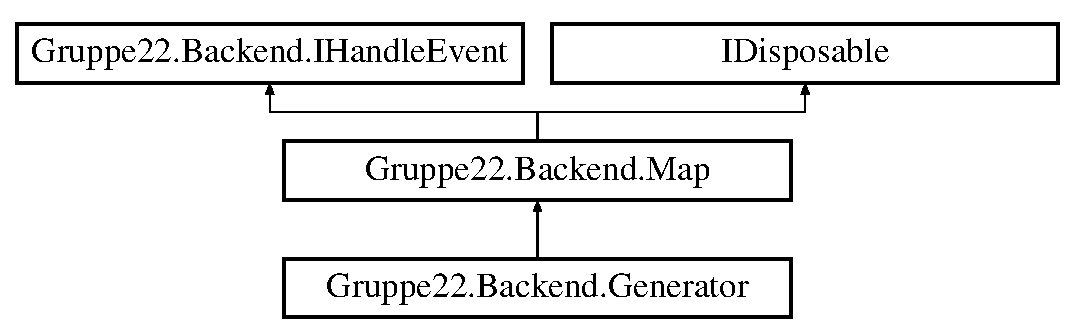
\includegraphics[height=3.000000cm]{class_gruppe22_1_1_backend_1_1_map}
\end{center}
\end{figure}
\subsection*{Öffentliche Methoden}
\begin{DoxyCompactItemize}
\item 
void \hyperlink{class_gruppe22_1_1_backend_1_1_map_a3f3723458566403e40673d4e757efb76}{Update} (Game\-Time game\-Time)
\begin{DoxyCompactList}\small\item\em Refresh tiles which do something (traps, enemies, N\-P\-Cs) \end{DoxyCompactList}\item 
void \hyperlink{class_gruppe22_1_1_backend_1_1_map_a120d2585d2cc5279322670a1274c820a}{Add\-Actor} (\hyperlink{class_gruppe22_1_1_backend_1_1_item}{Item} item, \hyperlink{class_gruppe22_1_1_backend_1_1_coords}{Backend.\-Coords} from)
\begin{DoxyCompactList}\small\item\em Add an actor to a tile \end{DoxyCompactList}\item 
void \hyperlink{class_gruppe22_1_1_backend_1_1_map_a0a3ac3d6dc5d341c9d1ebd9348d8db7a}{Uncover} (\hyperlink{class_gruppe22_1_1_backend_1_1_coords}{Coords} coords, int radius=4)
\item 
void \hyperlink{class_gruppe22_1_1_backend_1_1_map_ab7a2c3d607228ddb4aca3f28d6802f5a}{Move\-Actor} (\hyperlink{class_gruppe22_1_1_backend_1_1_actor}{Actor} actor, \hyperlink{namespace_gruppe22_1_1_backend_a2d53d5d14b8ea0951ba6971e5da1ebf5}{Direction} dir)
\begin{DoxyCompactList}\small\item\em Move an actor on the map in a specified direction (does not check for walls -\/ use Can\-Move) \end{DoxyCompactList}\item 
void \hyperlink{class_gruppe22_1_1_backend_1_1_map_a1d4d36a2ab918a0c37db26195508a0e5}{Add\-Item} (\hyperlink{class_gruppe22_1_1_backend_1_1_item}{Item} item, \hyperlink{class_gruppe22_1_1_backend_1_1_coords}{Backend.\-Coords} to)
\begin{DoxyCompactList}\small\item\em Add an item to a tile \end{DoxyCompactList}\item 
void \hyperlink{class_gruppe22_1_1_backend_1_1_map_a2bb2e356f5d269823152b90b6460dc96}{Move\-Item} (\hyperlink{class_gruppe22_1_1_backend_1_1_item}{Item} item, \hyperlink{class_gruppe22_1_1_backend_1_1_coords}{Backend.\-Coords} from, \hyperlink{namespace_gruppe22_1_1_backend_a2d53d5d14b8ea0951ba6971e5da1ebf5}{Direction} dir)
\begin{DoxyCompactList}\small\item\em Move an item on the map (not carried by an actor) in a specified direction \end{DoxyCompactList}\item 
\hyperlink{class_gruppe22_1_1_backend_1_1_coords}{Backend.\-Coords} \hyperlink{class_gruppe22_1_1_backend_1_1_map_aedf8ea673120929f8ad213d12441cd46}{Closest\-Enemy} (\hyperlink{class_gruppe22_1_1_backend_1_1_coords}{Coords} coords, int radius=4, bool include\-Player=true, bool include\-N\-P\-C=true, bool include\-Enemy=true)
\begin{DoxyCompactList}\small\item\em Get coordinates for closest enemy within a specified radius \end{DoxyCompactList}\item 
void \hyperlink{class_gruppe22_1_1_backend_1_1_map_a81e7cdb072bbd70c12ec23c76ce0cc3a}{Path\-To} (\hyperlink{class_gruppe22_1_1_backend_1_1_coords}{Coords} from, \hyperlink{class_gruppe22_1_1_backend_1_1_coords}{Backend.\-Coords} to, out List$<$ \hyperlink{class_gruppe22_1_1_backend_1_1_coords}{Coords} $>$ result, ref Sorted\-Set$<$ \hyperlink{class_gruppe22_1_1_backend_1_1_coords}{Coords} $>$ visited, int maxlength=20, string indent=\char`\"{}\char`\"{})
\item 
\hyperlink{class_gruppe22_1_1_backend_1_1_coords}{Backend.\-Coords} \hyperlink{class_gruppe22_1_1_backend_1_1_map_a186008c8dbdf442c4753dcf9eace5b58}{Get\-Checkpoint\-Coords} ()
\item 
\hyperlink{class_gruppe22_1_1_backend_1_1_floor_tile}{Floor\-Tile} \hyperlink{class_gruppe22_1_1_backend_1_1_map_a6b3eb978a3e4230531ee1f23a0f511b4}{Tile\-By\-Coords} (\hyperlink{class_gruppe22_1_1_backend_1_1_coords}{Coords} coords)
\item 
void \hyperlink{class_gruppe22_1_1_backend_1_1_map_a0c7963e738e6441b87c75a62381d95fd}{Remove\-Actor} (int x, int y)
\item 
int \hyperlink{class_gruppe22_1_1_backend_1_1_map_a87cb732700403985727f2535ecc3f955}{first\-Actor\-I\-D} (int x, int y)
\item 
bool \hyperlink{class_gruppe22_1_1_backend_1_1_map_afd4780d14e0ebb8dbd087b0a5d6cfbb9}{Can\-Move} (\hyperlink{class_gruppe22_1_1_backend_1_1_coords}{Coords} current\-Pos, \hyperlink{namespace_gruppe22_1_1_backend_a2d53d5d14b8ea0951ba6971e5da1ebf5}{Direction} dir)
\begin{DoxyCompactList}\small\item\em Check whether it is possible to move from a certain place on a map in a certain direction \end{DoxyCompactList}\item 
virtual void \hyperlink{class_gruppe22_1_1_backend_1_1_map_af3d260b8e5fb50958d07d99e171891d1}{Handle\-Event} (bool Down\-Stream, \hyperlink{namespace_gruppe22_1_1_backend_ab56df91bb0bdafa1ea978e552209ce73}{Events} event\-I\-D, params object\mbox{[}$\,$\mbox{]} data)
\item 
void \hyperlink{class_gruppe22_1_1_backend_1_1_map_ae5bf2ecbd364c82ae01c10b33ad8350a}{Load} (string filename, \hyperlink{class_gruppe22_1_1_backend_1_1_coords}{Backend.\-Coords} player=null)
\begin{DoxyCompactList}\small\item\em Load a map from a file \end{DoxyCompactList}\item 
void \hyperlink{class_gruppe22_1_1_backend_1_1_map_af5841f0eb6d27b7196056cfea1097141}{Debug\-Map} ()
\item 
virtual void \hyperlink{class_gruppe22_1_1_backend_1_1_map_ab1fe0990776579437497c699222253db}{Save} (string filename)
\begin{DoxyCompactList}\small\item\em Write the current map to a file \end{DoxyCompactList}\item 
\hyperlink{class_gruppe22_1_1_backend_1_1_map_ae43adfadc340541f54d6584f6851eb8e}{Map} (Content\-Manager content)
\item 
\hyperlink{class_gruppe22_1_1_backend_1_1_map_aa498945697ea3156633c5f1243fa2adc}{Map} (Content\-Manager content, object parent, string filename=\char`\"{}\char`\"{}, \hyperlink{class_gruppe22_1_1_backend_1_1_coords}{Backend.\-Coords} player\-Pos=null)
\begin{DoxyCompactList}\small\item\em Constructor for using a previously saved map \end{DoxyCompactList}\item 
virtual void \hyperlink{class_gruppe22_1_1_backend_1_1_map_a1a656c9f7104699b2736fdcc156615d3}{Dispose} ()
\end{DoxyCompactItemize}
\subsection*{Öffentliche, statische Methoden}
\begin{DoxyCompactItemize}
\item 
static \hyperlink{namespace_gruppe22_1_1_backend_a2d53d5d14b8ea0951ba6971e5da1ebf5}{Direction} \hyperlink{class_gruppe22_1_1_backend_1_1_map_ab84aa5963511604d27923fd9b7194d0f}{Which\-Way\-Is} (\hyperlink{class_gruppe22_1_1_backend_1_1_coords}{Coords} from, \hyperlink{class_gruppe22_1_1_backend_1_1_coords}{Backend.\-Coords} to, bool Direct\-Only=false)
\item 
static \hyperlink{namespace_gruppe22_1_1_backend_a2d53d5d14b8ea0951ba6971e5da1ebf5}{Direction} \hyperlink{class_gruppe22_1_1_backend_1_1_map_a90ad354d8da1ed9aa2cfac631edc864a}{Opposite\-Direction} (\hyperlink{namespace_gruppe22_1_1_backend_a2d53d5d14b8ea0951ba6971e5da1ebf5}{Direction} dir)
\item 
static \hyperlink{class_gruppe22_1_1_backend_1_1_coords}{Backend.\-Coords} \hyperlink{class_gruppe22_1_1_backend_1_1_map_a81136519b96adecb02bfd5552f5b55d3}{Direction\-Tile} (\hyperlink{class_gruppe22_1_1_backend_1_1_coords}{Coords} start, \hyperlink{namespace_gruppe22_1_1_backend_a2d53d5d14b8ea0951ba6971e5da1ebf5}{Direction} dir)
\item 
static \hyperlink{namespace_gruppe22_1_1_backend_a2d53d5d14b8ea0951ba6971e5da1ebf5}{Direction} \hyperlink{class_gruppe22_1_1_backend_1_1_map_ad56a1c4f4d9e9b1feb66d631e807ce56}{Next\-Direction} (\hyperlink{namespace_gruppe22_1_1_backend_a2d53d5d14b8ea0951ba6971e5da1ebf5}{Direction} dir, bool direct\-Only=false)
\item 
static List$<$ \hyperlink{class_gruppe22_1_1_backend_1_1_exit}{Exit} $>$ \hyperlink{class_gruppe22_1_1_backend_1_1_map_aaa0f3a0e9da112f1e60e04b5e2668bef}{Exit\-To\-Entry} (int To\-Room, List$<$ \hyperlink{class_gruppe22_1_1_backend_1_1_exit}{Exit} $>$ \hyperlink{class_gruppe22_1_1_backend_1_1_map_a0dc104d0e3f5896a272e4ed47dd79378}{exits})
\end{DoxyCompactItemize}
\subsection*{Geschützte Attribute}
\begin{DoxyCompactItemize}
\item 
Content\-Manager \hyperlink{class_gruppe22_1_1_backend_1_1_map_a477dd82902079fe3e40bedf22dbf2055}{\-\_\-content}
\item 
int \hyperlink{class_gruppe22_1_1_backend_1_1_map_a90048a67b858c4e4e5e3937785a59c83}{\-\_\-level}
\item 
string \hyperlink{class_gruppe22_1_1_backend_1_1_map_a4848f9eaed6a4fb65f88bd3b72e2d8f0}{\-\_\-name}
\item 
string \hyperlink{class_gruppe22_1_1_backend_1_1_map_a6c2e2b3369e1d2f793ae1c09d625a8ad}{\-\_\-dungeonname}
\item 
string \hyperlink{class_gruppe22_1_1_backend_1_1_map_aa963f4d1f06aa5722e961a7674828910}{\-\_\-wall\-File} = \char`\"{}wall1\char`\"{}
\item 
string \hyperlink{class_gruppe22_1_1_backend_1_1_map_a244299d80c512876e41c641aafa5effc}{\-\_\-floor\-File} = \char`\"{}floor1\char`\"{}
\item 
int \hyperlink{class_gruppe22_1_1_backend_1_1_map_ad75386d3edea7cb43bbf558742a5824e}{\-\_\-light}
\item 
string \hyperlink{class_gruppe22_1_1_backend_1_1_map_a99cac5327d78e72ced96f0dad20060cf}{\-\_\-music} = \char`\"{}level1\char`\"{}
\item 
int \hyperlink{class_gruppe22_1_1_backend_1_1_map_a09dec3f5d4010c7f0f3578e5de84d01b}{\-\_\-id}
\item 
List$<$ List$<$ \hyperlink{class_gruppe22_1_1_backend_1_1_floor_tile}{Floor\-Tile} $>$ $>$ \hyperlink{class_gruppe22_1_1_backend_1_1_map_a50c1a30d7d1c705375416767a474aa36}{\-\_\-tiles} = null
\begin{DoxyCompactList}\small\item\em A two dimensional list of tiles \end{DoxyCompactList}\item 
int \hyperlink{class_gruppe22_1_1_backend_1_1_map_a18b255b6ba29200aa83cd246ae8e3427}{\-\_\-width} = 10
\begin{DoxyCompactList}\small\item\em Internal current width \end{DoxyCompactList}\item 
List$<$ \hyperlink{class_gruppe22_1_1_backend_1_1_exit}{Exit} $>$ \hyperlink{class_gruppe22_1_1_backend_1_1_map_a57a44f95cc20e9516fb6d0ae805b68df}{\-\_\-exits}
\item 
int \hyperlink{class_gruppe22_1_1_backend_1_1_map_a69879990b9ce22a9fa0d31454d068b32}{\-\_\-height} = 10
\begin{DoxyCompactList}\small\item\em Internal current height \end{DoxyCompactList}\item 
List$<$ \hyperlink{class_gruppe22_1_1_backend_1_1_actor}{Actor} $>$ \hyperlink{class_gruppe22_1_1_backend_1_1_map_a29deb43269ce0e3dd577aafcd28aeb88}{\-\_\-actors} = null
\begin{DoxyCompactList}\small\item\em A list of Actors in the current room \end{DoxyCompactList}\item 
List$<$ \hyperlink{class_gruppe22_1_1_backend_1_1_item}{Item} $>$ \hyperlink{class_gruppe22_1_1_backend_1_1_map_a07ce05356ba78ac1470d64e0c736e190}{\-\_\-items} = null
\item 
List$<$ \hyperlink{class_gruppe22_1_1_backend_1_1_coords}{Coords} $>$ \hyperlink{class_gruppe22_1_1_backend_1_1_map_a1c8b19d3884fe44b1714ebec0256ce2a}{\-\_\-update\-Tiles} = null
\end{DoxyCompactItemize}
\subsection*{Propertys}
\begin{DoxyCompactItemize}
\item 
int \hyperlink{class_gruppe22_1_1_backend_1_1_map_abf7263c43d22ca634eceba89c06904cf}{level}\hspace{0.3cm}{\ttfamily  \mbox{[}get, set\mbox{]}}
\item 
string \hyperlink{class_gruppe22_1_1_backend_1_1_map_ae0e576fd7e8d25a3eb0370f2bcc896e1}{floor\-File}\hspace{0.3cm}{\ttfamily  \mbox{[}get, set\mbox{]}}
\item 
string \hyperlink{class_gruppe22_1_1_backend_1_1_map_af94c194982941748ccc41e58a2398691}{music}\hspace{0.3cm}{\ttfamily  \mbox{[}get, set\mbox{]}}
\item 
string \hyperlink{class_gruppe22_1_1_backend_1_1_map_ac30d110dd5617ce4ee1f0cab607ea6e8}{wall\-File}\hspace{0.3cm}{\ttfamily  \mbox{[}get, set\mbox{]}}
\item 
int \hyperlink{class_gruppe22_1_1_backend_1_1_map_a520dd5d828f2d1d0459736fe6bd09831}{light}\hspace{0.3cm}{\ttfamily  \mbox{[}get, set\mbox{]}}
\item 
string \hyperlink{class_gruppe22_1_1_backend_1_1_map_a7829a94426d54e43019423f88a7cec59}{name}\hspace{0.3cm}{\ttfamily  \mbox{[}get, set\mbox{]}}
\item 
string \hyperlink{class_gruppe22_1_1_backend_1_1_map_a76814bb49c2210b400230b9ee530010f}{dungeonname}\hspace{0.3cm}{\ttfamily  \mbox{[}get, set\mbox{]}}
\item 
List$<$ \hyperlink{class_gruppe22_1_1_backend_1_1_coords}{Coords} $>$ \hyperlink{class_gruppe22_1_1_backend_1_1_map_a33e42ed0b62ddb58ce402fb6fc455fdb}{update\-Tiles}\hspace{0.3cm}{\ttfamily  \mbox{[}get\mbox{]}}
\item 
int \hyperlink{class_gruppe22_1_1_backend_1_1_map_a31168190229d5fdaad90a0e27d41ef1a}{id}\hspace{0.3cm}{\ttfamily  \mbox{[}get, set\mbox{]}}
\item 
List$<$ \hyperlink{class_gruppe22_1_1_backend_1_1_actor}{Actor} $>$ \hyperlink{class_gruppe22_1_1_backend_1_1_map_a5b7ce0cacb479c6590d249aae60138fd}{actors}\hspace{0.3cm}{\ttfamily  \mbox{[}get, set\mbox{]}}
\item 
List$<$ \hyperlink{class_gruppe22_1_1_backend_1_1_exit}{Exit} $>$ \hyperlink{class_gruppe22_1_1_backend_1_1_map_a0dc104d0e3f5896a272e4ed47dd79378}{exits}\hspace{0.3cm}{\ttfamily  \mbox{[}get, set\mbox{]}}
\item 
List$<$ \hyperlink{class_gruppe22_1_1_backend_1_1_item}{Item} $>$ \hyperlink{class_gruppe22_1_1_backend_1_1_map_a91a89a011cd659affbbb00ea924211ca}{items}\hspace{0.3cm}{\ttfamily  \mbox{[}get, set\mbox{]}}
\item 
int \hyperlink{class_gruppe22_1_1_backend_1_1_map_ae185d7c51dd35311f6065044e603e81f}{width}\hspace{0.3cm}{\ttfamily  \mbox{[}get, set\mbox{]}}
\begin{DoxyCompactList}\small\item\em Current Width of the maze \end{DoxyCompactList}\item 
int \hyperlink{class_gruppe22_1_1_backend_1_1_map_aef59f2269d64d10b35acbabb6461fa55}{height}\hspace{0.3cm}{\ttfamily  \mbox{[}get, set\mbox{]}}
\begin{DoxyCompactList}\small\item\em Current Height of the maze \end{DoxyCompactList}\item 
List$<$ \hyperlink{class_gruppe22_1_1_backend_1_1_coords}{Coords} $>$ \hyperlink{class_gruppe22_1_1_backend_1_1_map_a186af3927e65a77740f619513dd2c60a}{actor\-Positions}\hspace{0.3cm}{\ttfamily  \mbox{[}get\mbox{]}}
\begin{DoxyCompactList}\small\item\em A list of the current position of every actor \end{DoxyCompactList}\item 
\hyperlink{class_gruppe22_1_1_backend_1_1_floor_tile}{Floor\-Tile} \hyperlink{class_gruppe22_1_1_backend_1_1_map_ac19e7d998d1c4befe3f1129939fd6b74}{this\mbox{[}\-Coords coords\mbox{]}}\hspace{0.3cm}{\ttfamily  \mbox{[}get, set\mbox{]}}
\begin{DoxyCompactList}\small\item\em Get the tile at coordinates x and y \end{DoxyCompactList}\item 
\hyperlink{class_gruppe22_1_1_backend_1_1_floor_tile}{Floor\-Tile} \hyperlink{class_gruppe22_1_1_backend_1_1_map_a51c56c902b3c7d2ee1e324b59ee89f8a}{this\mbox{[}int x, int y\mbox{]}}\hspace{0.3cm}{\ttfamily  \mbox{[}get, set\mbox{]}}
\begin{DoxyCompactList}\small\item\em Get the tile at coordinates x and y \end{DoxyCompactList}\end{DoxyCompactItemize}


\subsection{Beschreibung der Konstruktoren und Destruktoren}
\hypertarget{class_gruppe22_1_1_backend_1_1_map_ae43adfadc340541f54d6584f6851eb8e}{\index{Gruppe22\-::\-Backend\-::\-Map@{Gruppe22\-::\-Backend\-::\-Map}!Map@{Map}}
\index{Map@{Map}!Gruppe22::Backend::Map@{Gruppe22\-::\-Backend\-::\-Map}}
\subsubsection[{Map}]{\setlength{\rightskip}{0pt plus 5cm}Gruppe22.\-Backend.\-Map.\-Map (
\begin{DoxyParamCaption}
\item[{Content\-Manager}]{content}
\end{DoxyParamCaption}
)}}\label{class_gruppe22_1_1_backend_1_1_map_ae43adfadc340541f54d6584f6851eb8e}
\hypertarget{class_gruppe22_1_1_backend_1_1_map_aa498945697ea3156633c5f1243fa2adc}{\index{Gruppe22\-::\-Backend\-::\-Map@{Gruppe22\-::\-Backend\-::\-Map}!Map@{Map}}
\index{Map@{Map}!Gruppe22::Backend::Map@{Gruppe22\-::\-Backend\-::\-Map}}
\subsubsection[{Map}]{\setlength{\rightskip}{0pt plus 5cm}Gruppe22.\-Backend.\-Map.\-Map (
\begin{DoxyParamCaption}
\item[{Content\-Manager}]{content, }
\item[{object}]{parent, }
\item[{string}]{filename = {\ttfamily \char`\"{}\char`\"{}}, }
\item[{{\bf Backend.\-Coords}}]{player\-Pos = {\ttfamily null}}
\end{DoxyParamCaption}
)}}\label{class_gruppe22_1_1_backend_1_1_map_aa498945697ea3156633c5f1243fa2adc}


Constructor for using a previously saved map 


\begin{DoxyParams}{Parameter}
{\em filename} & \\
\hline
\end{DoxyParams}


\subsection{Dokumentation der Elementfunktionen}
\hypertarget{class_gruppe22_1_1_backend_1_1_map_a120d2585d2cc5279322670a1274c820a}{\index{Gruppe22\-::\-Backend\-::\-Map@{Gruppe22\-::\-Backend\-::\-Map}!Add\-Actor@{Add\-Actor}}
\index{Add\-Actor@{Add\-Actor}!Gruppe22::Backend::Map@{Gruppe22\-::\-Backend\-::\-Map}}
\subsubsection[{Add\-Actor}]{\setlength{\rightskip}{0pt plus 5cm}void Gruppe22.\-Backend.\-Map.\-Add\-Actor (
\begin{DoxyParamCaption}
\item[{{\bf Item}}]{item, }
\item[{{\bf Backend.\-Coords}}]{from}
\end{DoxyParamCaption}
)}}\label{class_gruppe22_1_1_backend_1_1_map_a120d2585d2cc5279322670a1274c820a}


Add an actor to a tile 


\begin{DoxyParams}{Parameter}
{\em item} & \\
\hline
{\em from} & \\
\hline
\end{DoxyParams}
\hypertarget{class_gruppe22_1_1_backend_1_1_map_a1d4d36a2ab918a0c37db26195508a0e5}{\index{Gruppe22\-::\-Backend\-::\-Map@{Gruppe22\-::\-Backend\-::\-Map}!Add\-Item@{Add\-Item}}
\index{Add\-Item@{Add\-Item}!Gruppe22::Backend::Map@{Gruppe22\-::\-Backend\-::\-Map}}
\subsubsection[{Add\-Item}]{\setlength{\rightskip}{0pt plus 5cm}void Gruppe22.\-Backend.\-Map.\-Add\-Item (
\begin{DoxyParamCaption}
\item[{{\bf Item}}]{item, }
\item[{{\bf Backend.\-Coords}}]{to}
\end{DoxyParamCaption}
)}}\label{class_gruppe22_1_1_backend_1_1_map_a1d4d36a2ab918a0c37db26195508a0e5}


Add an item to a tile 


\begin{DoxyParams}{Parameter}
{\em actor} & \\
\hline
{\em to} & \\
\hline
\end{DoxyParams}
\hypertarget{class_gruppe22_1_1_backend_1_1_map_afd4780d14e0ebb8dbd087b0a5d6cfbb9}{\index{Gruppe22\-::\-Backend\-::\-Map@{Gruppe22\-::\-Backend\-::\-Map}!Can\-Move@{Can\-Move}}
\index{Can\-Move@{Can\-Move}!Gruppe22::Backend::Map@{Gruppe22\-::\-Backend\-::\-Map}}
\subsubsection[{Can\-Move}]{\setlength{\rightskip}{0pt plus 5cm}bool Gruppe22.\-Backend.\-Map.\-Can\-Move (
\begin{DoxyParamCaption}
\item[{{\bf Coords}}]{current\-Pos, }
\item[{{\bf Direction}}]{dir}
\end{DoxyParamCaption}
)}}\label{class_gruppe22_1_1_backend_1_1_map_afd4780d14e0ebb8dbd087b0a5d6cfbb9}


Check whether it is possible to move from a certain place on a map in a certain direction 


\begin{DoxyParams}{Parameter}
{\em current\-Pos} & Coordinates on current map\\
\hline
{\em dir} & Direction to move to\\
\hline
\end{DoxyParams}
\begin{DoxyReturn}{Rückgabe}
true if move is allowed
\end{DoxyReturn}
\hypertarget{class_gruppe22_1_1_backend_1_1_map_aedf8ea673120929f8ad213d12441cd46}{\index{Gruppe22\-::\-Backend\-::\-Map@{Gruppe22\-::\-Backend\-::\-Map}!Closest\-Enemy@{Closest\-Enemy}}
\index{Closest\-Enemy@{Closest\-Enemy}!Gruppe22::Backend::Map@{Gruppe22\-::\-Backend\-::\-Map}}
\subsubsection[{Closest\-Enemy}]{\setlength{\rightskip}{0pt plus 5cm}{\bf Backend.\-Coords} Gruppe22.\-Backend.\-Map.\-Closest\-Enemy (
\begin{DoxyParamCaption}
\item[{{\bf Coords}}]{coords, }
\item[{int}]{radius = {\ttfamily 4}, }
\item[{bool}]{include\-Player = {\ttfamily true}, }
\item[{bool}]{include\-N\-P\-C = {\ttfamily true}, }
\item[{bool}]{include\-Enemy = {\ttfamily true}}
\end{DoxyParamCaption}
)}}\label{class_gruppe22_1_1_backend_1_1_map_aedf8ea673120929f8ad213d12441cd46}


Get coordinates for closest enemy within a specified radius 


\begin{DoxyParams}{Parameter}
{\em coords} & \\
\hline
{\em radius} & \\
\hline
{\em include\-Player} & \\
\hline
{\em include\-N\-P\-C} & \\
\hline
{\em include\-Enemy} & \\
\hline
\end{DoxyParams}
\begin{DoxyReturn}{Rückgabe}

\end{DoxyReturn}
\hypertarget{class_gruppe22_1_1_backend_1_1_map_af5841f0eb6d27b7196056cfea1097141}{\index{Gruppe22\-::\-Backend\-::\-Map@{Gruppe22\-::\-Backend\-::\-Map}!Debug\-Map@{Debug\-Map}}
\index{Debug\-Map@{Debug\-Map}!Gruppe22::Backend::Map@{Gruppe22\-::\-Backend\-::\-Map}}
\subsubsection[{Debug\-Map}]{\setlength{\rightskip}{0pt plus 5cm}void Gruppe22.\-Backend.\-Map.\-Debug\-Map (
\begin{DoxyParamCaption}
{}
\end{DoxyParamCaption}
)}}\label{class_gruppe22_1_1_backend_1_1_map_af5841f0eb6d27b7196056cfea1097141}
\hypertarget{class_gruppe22_1_1_backend_1_1_map_a81136519b96adecb02bfd5552f5b55d3}{\index{Gruppe22\-::\-Backend\-::\-Map@{Gruppe22\-::\-Backend\-::\-Map}!Direction\-Tile@{Direction\-Tile}}
\index{Direction\-Tile@{Direction\-Tile}!Gruppe22::Backend::Map@{Gruppe22\-::\-Backend\-::\-Map}}
\subsubsection[{Direction\-Tile}]{\setlength{\rightskip}{0pt plus 5cm}static {\bf Backend.\-Coords} Gruppe22.\-Backend.\-Map.\-Direction\-Tile (
\begin{DoxyParamCaption}
\item[{{\bf Coords}}]{start, }
\item[{{\bf Direction}}]{dir}
\end{DoxyParamCaption}
)\hspace{0.3cm}{\ttfamily [static]}}}\label{class_gruppe22_1_1_backend_1_1_map_a81136519b96adecb02bfd5552f5b55d3}
\hypertarget{class_gruppe22_1_1_backend_1_1_map_a1a656c9f7104699b2736fdcc156615d3}{\index{Gruppe22\-::\-Backend\-::\-Map@{Gruppe22\-::\-Backend\-::\-Map}!Dispose@{Dispose}}
\index{Dispose@{Dispose}!Gruppe22::Backend::Map@{Gruppe22\-::\-Backend\-::\-Map}}
\subsubsection[{Dispose}]{\setlength{\rightskip}{0pt plus 5cm}virtual void Gruppe22.\-Backend.\-Map.\-Dispose (
\begin{DoxyParamCaption}
{}
\end{DoxyParamCaption}
)\hspace{0.3cm}{\ttfamily [virtual]}}}\label{class_gruppe22_1_1_backend_1_1_map_a1a656c9f7104699b2736fdcc156615d3}
\hypertarget{class_gruppe22_1_1_backend_1_1_map_aaa0f3a0e9da112f1e60e04b5e2668bef}{\index{Gruppe22\-::\-Backend\-::\-Map@{Gruppe22\-::\-Backend\-::\-Map}!Exit\-To\-Entry@{Exit\-To\-Entry}}
\index{Exit\-To\-Entry@{Exit\-To\-Entry}!Gruppe22::Backend::Map@{Gruppe22\-::\-Backend\-::\-Map}}
\subsubsection[{Exit\-To\-Entry}]{\setlength{\rightskip}{0pt plus 5cm}static List$<${\bf Exit}$>$ Gruppe22.\-Backend.\-Map.\-Exit\-To\-Entry (
\begin{DoxyParamCaption}
\item[{int}]{To\-Room, }
\item[{List$<$ {\bf Exit} $>$}]{exits}
\end{DoxyParamCaption}
)\hspace{0.3cm}{\ttfamily [static]}}}\label{class_gruppe22_1_1_backend_1_1_map_aaa0f3a0e9da112f1e60e04b5e2668bef}
\hypertarget{class_gruppe22_1_1_backend_1_1_map_a87cb732700403985727f2535ecc3f955}{\index{Gruppe22\-::\-Backend\-::\-Map@{Gruppe22\-::\-Backend\-::\-Map}!first\-Actor\-I\-D@{first\-Actor\-I\-D}}
\index{first\-Actor\-I\-D@{first\-Actor\-I\-D}!Gruppe22::Backend::Map@{Gruppe22\-::\-Backend\-::\-Map}}
\subsubsection[{first\-Actor\-I\-D}]{\setlength{\rightskip}{0pt plus 5cm}int Gruppe22.\-Backend.\-Map.\-first\-Actor\-I\-D (
\begin{DoxyParamCaption}
\item[{int}]{x, }
\item[{int}]{y}
\end{DoxyParamCaption}
)}}\label{class_gruppe22_1_1_backend_1_1_map_a87cb732700403985727f2535ecc3f955}
\hypertarget{class_gruppe22_1_1_backend_1_1_map_a186008c8dbdf442c4753dcf9eace5b58}{\index{Gruppe22\-::\-Backend\-::\-Map@{Gruppe22\-::\-Backend\-::\-Map}!Get\-Checkpoint\-Coords@{Get\-Checkpoint\-Coords}}
\index{Get\-Checkpoint\-Coords@{Get\-Checkpoint\-Coords}!Gruppe22::Backend::Map@{Gruppe22\-::\-Backend\-::\-Map}}
\subsubsection[{Get\-Checkpoint\-Coords}]{\setlength{\rightskip}{0pt plus 5cm}{\bf Backend.\-Coords} Gruppe22.\-Backend.\-Map.\-Get\-Checkpoint\-Coords (
\begin{DoxyParamCaption}
{}
\end{DoxyParamCaption}
)}}\label{class_gruppe22_1_1_backend_1_1_map_a186008c8dbdf442c4753dcf9eace5b58}
\hypertarget{class_gruppe22_1_1_backend_1_1_map_af3d260b8e5fb50958d07d99e171891d1}{\index{Gruppe22\-::\-Backend\-::\-Map@{Gruppe22\-::\-Backend\-::\-Map}!Handle\-Event@{Handle\-Event}}
\index{Handle\-Event@{Handle\-Event}!Gruppe22::Backend::Map@{Gruppe22\-::\-Backend\-::\-Map}}
\subsubsection[{Handle\-Event}]{\setlength{\rightskip}{0pt plus 5cm}virtual void Gruppe22.\-Backend.\-Map.\-Handle\-Event (
\begin{DoxyParamCaption}
\item[{bool}]{Down\-Stream, }
\item[{{\bf Events}}]{event\-I\-D, }
\item[{params object\mbox{[}$\,$\mbox{]}}]{data}
\end{DoxyParamCaption}
)\hspace{0.3cm}{\ttfamily [virtual]}}}\label{class_gruppe22_1_1_backend_1_1_map_af3d260b8e5fb50958d07d99e171891d1}
\hypertarget{class_gruppe22_1_1_backend_1_1_map_ae5bf2ecbd364c82ae01c10b33ad8350a}{\index{Gruppe22\-::\-Backend\-::\-Map@{Gruppe22\-::\-Backend\-::\-Map}!Load@{Load}}
\index{Load@{Load}!Gruppe22::Backend::Map@{Gruppe22\-::\-Backend\-::\-Map}}
\subsubsection[{Load}]{\setlength{\rightskip}{0pt plus 5cm}void Gruppe22.\-Backend.\-Map.\-Load (
\begin{DoxyParamCaption}
\item[{string}]{filename, }
\item[{{\bf Backend.\-Coords}}]{player = {\ttfamily null}}
\end{DoxyParamCaption}
)}}\label{class_gruppe22_1_1_backend_1_1_map_ae5bf2ecbd364c82ae01c10b33ad8350a}


Load a map from a file 


\begin{DoxyParams}{Parameter}
{\em filename} & The filename to read from\\
\hline
{\em player} & The starting position on the loaded map\\
\hline
\end{DoxyParams}
\hypertarget{class_gruppe22_1_1_backend_1_1_map_ab7a2c3d607228ddb4aca3f28d6802f5a}{\index{Gruppe22\-::\-Backend\-::\-Map@{Gruppe22\-::\-Backend\-::\-Map}!Move\-Actor@{Move\-Actor}}
\index{Move\-Actor@{Move\-Actor}!Gruppe22::Backend::Map@{Gruppe22\-::\-Backend\-::\-Map}}
\subsubsection[{Move\-Actor}]{\setlength{\rightskip}{0pt plus 5cm}void Gruppe22.\-Backend.\-Map.\-Move\-Actor (
\begin{DoxyParamCaption}
\item[{{\bf Actor}}]{actor, }
\item[{{\bf Direction}}]{dir}
\end{DoxyParamCaption}
)}}\label{class_gruppe22_1_1_backend_1_1_map_ab7a2c3d607228ddb4aca3f28d6802f5a}


Move an actor on the map in a specified direction (does not check for walls -\/ use Can\-Move) 


\begin{DoxyParams}{Parameter}
{\em actor} & \\
\hline
{\em from} & \\
\hline
{\em dir} & \\
\hline
\end{DoxyParams}
\hypertarget{class_gruppe22_1_1_backend_1_1_map_a2bb2e356f5d269823152b90b6460dc96}{\index{Gruppe22\-::\-Backend\-::\-Map@{Gruppe22\-::\-Backend\-::\-Map}!Move\-Item@{Move\-Item}}
\index{Move\-Item@{Move\-Item}!Gruppe22::Backend::Map@{Gruppe22\-::\-Backend\-::\-Map}}
\subsubsection[{Move\-Item}]{\setlength{\rightskip}{0pt plus 5cm}void Gruppe22.\-Backend.\-Map.\-Move\-Item (
\begin{DoxyParamCaption}
\item[{{\bf Item}}]{item, }
\item[{{\bf Backend.\-Coords}}]{from, }
\item[{{\bf Direction}}]{dir}
\end{DoxyParamCaption}
)}}\label{class_gruppe22_1_1_backend_1_1_map_a2bb2e356f5d269823152b90b6460dc96}


Move an item on the map (not carried by an actor) in a specified direction 


\begin{DoxyParams}{Parameter}
{\em item} & item to move\\
\hline
{\em from} & square from which to move item\\
\hline
{\em dir} & Direction to move to\\
\hline
\end{DoxyParams}
\hypertarget{class_gruppe22_1_1_backend_1_1_map_ad56a1c4f4d9e9b1feb66d631e807ce56}{\index{Gruppe22\-::\-Backend\-::\-Map@{Gruppe22\-::\-Backend\-::\-Map}!Next\-Direction@{Next\-Direction}}
\index{Next\-Direction@{Next\-Direction}!Gruppe22::Backend::Map@{Gruppe22\-::\-Backend\-::\-Map}}
\subsubsection[{Next\-Direction}]{\setlength{\rightskip}{0pt plus 5cm}static {\bf Direction} Gruppe22.\-Backend.\-Map.\-Next\-Direction (
\begin{DoxyParamCaption}
\item[{{\bf Direction}}]{dir, }
\item[{bool}]{direct\-Only = {\ttfamily false}}
\end{DoxyParamCaption}
)\hspace{0.3cm}{\ttfamily [static]}}}\label{class_gruppe22_1_1_backend_1_1_map_ad56a1c4f4d9e9b1feb66d631e807ce56}
\hypertarget{class_gruppe22_1_1_backend_1_1_map_a90ad354d8da1ed9aa2cfac631edc864a}{\index{Gruppe22\-::\-Backend\-::\-Map@{Gruppe22\-::\-Backend\-::\-Map}!Opposite\-Direction@{Opposite\-Direction}}
\index{Opposite\-Direction@{Opposite\-Direction}!Gruppe22::Backend::Map@{Gruppe22\-::\-Backend\-::\-Map}}
\subsubsection[{Opposite\-Direction}]{\setlength{\rightskip}{0pt plus 5cm}static {\bf Direction} Gruppe22.\-Backend.\-Map.\-Opposite\-Direction (
\begin{DoxyParamCaption}
\item[{{\bf Direction}}]{dir}
\end{DoxyParamCaption}
)\hspace{0.3cm}{\ttfamily [static]}}}\label{class_gruppe22_1_1_backend_1_1_map_a90ad354d8da1ed9aa2cfac631edc864a}
\hypertarget{class_gruppe22_1_1_backend_1_1_map_a81e7cdb072bbd70c12ec23c76ce0cc3a}{\index{Gruppe22\-::\-Backend\-::\-Map@{Gruppe22\-::\-Backend\-::\-Map}!Path\-To@{Path\-To}}
\index{Path\-To@{Path\-To}!Gruppe22::Backend::Map@{Gruppe22\-::\-Backend\-::\-Map}}
\subsubsection[{Path\-To}]{\setlength{\rightskip}{0pt plus 5cm}void Gruppe22.\-Backend.\-Map.\-Path\-To (
\begin{DoxyParamCaption}
\item[{{\bf Coords}}]{from, }
\item[{{\bf Backend.\-Coords}}]{to, }
\item[{out List$<$ {\bf Coords} $>$}]{result, }
\item[{ref Sorted\-Set$<$ {\bf Coords} $>$}]{visited, }
\item[{int}]{maxlength = {\ttfamily 20}, }
\item[{string}]{indent = {\ttfamily \char`\"{}\char`\"{}}}
\end{DoxyParamCaption}
)}}\label{class_gruppe22_1_1_backend_1_1_map_a81e7cdb072bbd70c12ec23c76ce0cc3a}
\hypertarget{class_gruppe22_1_1_backend_1_1_map_a0c7963e738e6441b87c75a62381d95fd}{\index{Gruppe22\-::\-Backend\-::\-Map@{Gruppe22\-::\-Backend\-::\-Map}!Remove\-Actor@{Remove\-Actor}}
\index{Remove\-Actor@{Remove\-Actor}!Gruppe22::Backend::Map@{Gruppe22\-::\-Backend\-::\-Map}}
\subsubsection[{Remove\-Actor}]{\setlength{\rightskip}{0pt plus 5cm}void Gruppe22.\-Backend.\-Map.\-Remove\-Actor (
\begin{DoxyParamCaption}
\item[{int}]{x, }
\item[{int}]{y}
\end{DoxyParamCaption}
)}}\label{class_gruppe22_1_1_backend_1_1_map_a0c7963e738e6441b87c75a62381d95fd}
\hypertarget{class_gruppe22_1_1_backend_1_1_map_ab1fe0990776579437497c699222253db}{\index{Gruppe22\-::\-Backend\-::\-Map@{Gruppe22\-::\-Backend\-::\-Map}!Save@{Save}}
\index{Save@{Save}!Gruppe22::Backend::Map@{Gruppe22\-::\-Backend\-::\-Map}}
\subsubsection[{Save}]{\setlength{\rightskip}{0pt plus 5cm}virtual void Gruppe22.\-Backend.\-Map.\-Save (
\begin{DoxyParamCaption}
\item[{string}]{filename}
\end{DoxyParamCaption}
)\hspace{0.3cm}{\ttfamily [virtual]}}}\label{class_gruppe22_1_1_backend_1_1_map_ab1fe0990776579437497c699222253db}


Write the current map to a file 


\begin{DoxyParams}{Parameter}
{\em filename} & The filename to write to\\
\hline
\end{DoxyParams}


Erneute Implementation in \hyperlink{class_gruppe22_1_1_backend_1_1_generator_ae0e94d668013ad78b8ed91f98009e488}{Gruppe22.\-Backend.\-Generator}.

\hypertarget{class_gruppe22_1_1_backend_1_1_map_a6b3eb978a3e4230531ee1f23a0f511b4}{\index{Gruppe22\-::\-Backend\-::\-Map@{Gruppe22\-::\-Backend\-::\-Map}!Tile\-By\-Coords@{Tile\-By\-Coords}}
\index{Tile\-By\-Coords@{Tile\-By\-Coords}!Gruppe22::Backend::Map@{Gruppe22\-::\-Backend\-::\-Map}}
\subsubsection[{Tile\-By\-Coords}]{\setlength{\rightskip}{0pt plus 5cm}{\bf Floor\-Tile} Gruppe22.\-Backend.\-Map.\-Tile\-By\-Coords (
\begin{DoxyParamCaption}
\item[{{\bf Coords}}]{coords}
\end{DoxyParamCaption}
)}}\label{class_gruppe22_1_1_backend_1_1_map_a6b3eb978a3e4230531ee1f23a0f511b4}
\hypertarget{class_gruppe22_1_1_backend_1_1_map_a0a3ac3d6dc5d341c9d1ebd9348d8db7a}{\index{Gruppe22\-::\-Backend\-::\-Map@{Gruppe22\-::\-Backend\-::\-Map}!Uncover@{Uncover}}
\index{Uncover@{Uncover}!Gruppe22::Backend::Map@{Gruppe22\-::\-Backend\-::\-Map}}
\subsubsection[{Uncover}]{\setlength{\rightskip}{0pt plus 5cm}void Gruppe22.\-Backend.\-Map.\-Uncover (
\begin{DoxyParamCaption}
\item[{{\bf Coords}}]{coords, }
\item[{int}]{radius = {\ttfamily 4}}
\end{DoxyParamCaption}
)}}\label{class_gruppe22_1_1_backend_1_1_map_a0a3ac3d6dc5d341c9d1ebd9348d8db7a}
\hypertarget{class_gruppe22_1_1_backend_1_1_map_a3f3723458566403e40673d4e757efb76}{\index{Gruppe22\-::\-Backend\-::\-Map@{Gruppe22\-::\-Backend\-::\-Map}!Update@{Update}}
\index{Update@{Update}!Gruppe22::Backend::Map@{Gruppe22\-::\-Backend\-::\-Map}}
\subsubsection[{Update}]{\setlength{\rightskip}{0pt plus 5cm}void Gruppe22.\-Backend.\-Map.\-Update (
\begin{DoxyParamCaption}
\item[{Game\-Time}]{game\-Time}
\end{DoxyParamCaption}
)}}\label{class_gruppe22_1_1_backend_1_1_map_a3f3723458566403e40673d4e757efb76}


Refresh tiles which do something (traps, enemies, N\-P\-Cs) 


\begin{DoxyParams}{Parameter}
{\em game\-Time} & \\
\hline
\end{DoxyParams}
\hypertarget{class_gruppe22_1_1_backend_1_1_map_ab84aa5963511604d27923fd9b7194d0f}{\index{Gruppe22\-::\-Backend\-::\-Map@{Gruppe22\-::\-Backend\-::\-Map}!Which\-Way\-Is@{Which\-Way\-Is}}
\index{Which\-Way\-Is@{Which\-Way\-Is}!Gruppe22::Backend::Map@{Gruppe22\-::\-Backend\-::\-Map}}
\subsubsection[{Which\-Way\-Is}]{\setlength{\rightskip}{0pt plus 5cm}static {\bf Direction} Gruppe22.\-Backend.\-Map.\-Which\-Way\-Is (
\begin{DoxyParamCaption}
\item[{{\bf Coords}}]{from, }
\item[{{\bf Backend.\-Coords}}]{to, }
\item[{bool}]{Direct\-Only = {\ttfamily false}}
\end{DoxyParamCaption}
)\hspace{0.3cm}{\ttfamily [static]}}}\label{class_gruppe22_1_1_backend_1_1_map_ab84aa5963511604d27923fd9b7194d0f}


\subsection{Dokumentation der Datenelemente}
\hypertarget{class_gruppe22_1_1_backend_1_1_map_a29deb43269ce0e3dd577aafcd28aeb88}{\index{Gruppe22\-::\-Backend\-::\-Map@{Gruppe22\-::\-Backend\-::\-Map}!\-\_\-actors@{\-\_\-actors}}
\index{\-\_\-actors@{\-\_\-actors}!Gruppe22::Backend::Map@{Gruppe22\-::\-Backend\-::\-Map}}
\subsubsection[{\-\_\-actors}]{\setlength{\rightskip}{0pt plus 5cm}List$<${\bf Actor}$>$ Gruppe22.\-Backend.\-Map.\-\_\-actors = null\hspace{0.3cm}{\ttfamily [protected]}}}\label{class_gruppe22_1_1_backend_1_1_map_a29deb43269ce0e3dd577aafcd28aeb88}


A list of Actors in the current room 

\hypertarget{class_gruppe22_1_1_backend_1_1_map_a477dd82902079fe3e40bedf22dbf2055}{\index{Gruppe22\-::\-Backend\-::\-Map@{Gruppe22\-::\-Backend\-::\-Map}!\-\_\-content@{\-\_\-content}}
\index{\-\_\-content@{\-\_\-content}!Gruppe22::Backend::Map@{Gruppe22\-::\-Backend\-::\-Map}}
\subsubsection[{\-\_\-content}]{\setlength{\rightskip}{0pt plus 5cm}Content\-Manager Gruppe22.\-Backend.\-Map.\-\_\-content\hspace{0.3cm}{\ttfamily [protected]}}}\label{class_gruppe22_1_1_backend_1_1_map_a477dd82902079fe3e40bedf22dbf2055}
\hypertarget{class_gruppe22_1_1_backend_1_1_map_a6c2e2b3369e1d2f793ae1c09d625a8ad}{\index{Gruppe22\-::\-Backend\-::\-Map@{Gruppe22\-::\-Backend\-::\-Map}!\-\_\-dungeonname@{\-\_\-dungeonname}}
\index{\-\_\-dungeonname@{\-\_\-dungeonname}!Gruppe22::Backend::Map@{Gruppe22\-::\-Backend\-::\-Map}}
\subsubsection[{\-\_\-dungeonname}]{\setlength{\rightskip}{0pt plus 5cm}string Gruppe22.\-Backend.\-Map.\-\_\-dungeonname\hspace{0.3cm}{\ttfamily [protected]}}}\label{class_gruppe22_1_1_backend_1_1_map_a6c2e2b3369e1d2f793ae1c09d625a8ad}
\hypertarget{class_gruppe22_1_1_backend_1_1_map_a57a44f95cc20e9516fb6d0ae805b68df}{\index{Gruppe22\-::\-Backend\-::\-Map@{Gruppe22\-::\-Backend\-::\-Map}!\-\_\-exits@{\-\_\-exits}}
\index{\-\_\-exits@{\-\_\-exits}!Gruppe22::Backend::Map@{Gruppe22\-::\-Backend\-::\-Map}}
\subsubsection[{\-\_\-exits}]{\setlength{\rightskip}{0pt plus 5cm}List$<${\bf Exit}$>$ Gruppe22.\-Backend.\-Map.\-\_\-exits\hspace{0.3cm}{\ttfamily [protected]}}}\label{class_gruppe22_1_1_backend_1_1_map_a57a44f95cc20e9516fb6d0ae805b68df}
\hypertarget{class_gruppe22_1_1_backend_1_1_map_a244299d80c512876e41c641aafa5effc}{\index{Gruppe22\-::\-Backend\-::\-Map@{Gruppe22\-::\-Backend\-::\-Map}!\-\_\-floor\-File@{\-\_\-floor\-File}}
\index{\-\_\-floor\-File@{\-\_\-floor\-File}!Gruppe22::Backend::Map@{Gruppe22\-::\-Backend\-::\-Map}}
\subsubsection[{\-\_\-floor\-File}]{\setlength{\rightskip}{0pt plus 5cm}string Gruppe22.\-Backend.\-Map.\-\_\-floor\-File = \char`\"{}floor1\char`\"{}\hspace{0.3cm}{\ttfamily [protected]}}}\label{class_gruppe22_1_1_backend_1_1_map_a244299d80c512876e41c641aafa5effc}
\hypertarget{class_gruppe22_1_1_backend_1_1_map_a69879990b9ce22a9fa0d31454d068b32}{\index{Gruppe22\-::\-Backend\-::\-Map@{Gruppe22\-::\-Backend\-::\-Map}!\-\_\-height@{\-\_\-height}}
\index{\-\_\-height@{\-\_\-height}!Gruppe22::Backend::Map@{Gruppe22\-::\-Backend\-::\-Map}}
\subsubsection[{\-\_\-height}]{\setlength{\rightskip}{0pt plus 5cm}int Gruppe22.\-Backend.\-Map.\-\_\-height = 10\hspace{0.3cm}{\ttfamily [protected]}}}\label{class_gruppe22_1_1_backend_1_1_map_a69879990b9ce22a9fa0d31454d068b32}


Internal current height 

\hypertarget{class_gruppe22_1_1_backend_1_1_map_a09dec3f5d4010c7f0f3578e5de84d01b}{\index{Gruppe22\-::\-Backend\-::\-Map@{Gruppe22\-::\-Backend\-::\-Map}!\-\_\-id@{\-\_\-id}}
\index{\-\_\-id@{\-\_\-id}!Gruppe22::Backend::Map@{Gruppe22\-::\-Backend\-::\-Map}}
\subsubsection[{\-\_\-id}]{\setlength{\rightskip}{0pt plus 5cm}int Gruppe22.\-Backend.\-Map.\-\_\-id\hspace{0.3cm}{\ttfamily [protected]}}}\label{class_gruppe22_1_1_backend_1_1_map_a09dec3f5d4010c7f0f3578e5de84d01b}
\hypertarget{class_gruppe22_1_1_backend_1_1_map_a07ce05356ba78ac1470d64e0c736e190}{\index{Gruppe22\-::\-Backend\-::\-Map@{Gruppe22\-::\-Backend\-::\-Map}!\-\_\-items@{\-\_\-items}}
\index{\-\_\-items@{\-\_\-items}!Gruppe22::Backend::Map@{Gruppe22\-::\-Backend\-::\-Map}}
\subsubsection[{\-\_\-items}]{\setlength{\rightskip}{0pt plus 5cm}List$<${\bf Item}$>$ Gruppe22.\-Backend.\-Map.\-\_\-items = null\hspace{0.3cm}{\ttfamily [protected]}}}\label{class_gruppe22_1_1_backend_1_1_map_a07ce05356ba78ac1470d64e0c736e190}
\hypertarget{class_gruppe22_1_1_backend_1_1_map_a90048a67b858c4e4e5e3937785a59c83}{\index{Gruppe22\-::\-Backend\-::\-Map@{Gruppe22\-::\-Backend\-::\-Map}!\-\_\-level@{\-\_\-level}}
\index{\-\_\-level@{\-\_\-level}!Gruppe22::Backend::Map@{Gruppe22\-::\-Backend\-::\-Map}}
\subsubsection[{\-\_\-level}]{\setlength{\rightskip}{0pt plus 5cm}int Gruppe22.\-Backend.\-Map.\-\_\-level\hspace{0.3cm}{\ttfamily [protected]}}}\label{class_gruppe22_1_1_backend_1_1_map_a90048a67b858c4e4e5e3937785a59c83}
\hypertarget{class_gruppe22_1_1_backend_1_1_map_ad75386d3edea7cb43bbf558742a5824e}{\index{Gruppe22\-::\-Backend\-::\-Map@{Gruppe22\-::\-Backend\-::\-Map}!\-\_\-light@{\-\_\-light}}
\index{\-\_\-light@{\-\_\-light}!Gruppe22::Backend::Map@{Gruppe22\-::\-Backend\-::\-Map}}
\subsubsection[{\-\_\-light}]{\setlength{\rightskip}{0pt plus 5cm}int Gruppe22.\-Backend.\-Map.\-\_\-light\hspace{0.3cm}{\ttfamily [protected]}}}\label{class_gruppe22_1_1_backend_1_1_map_ad75386d3edea7cb43bbf558742a5824e}
\hypertarget{class_gruppe22_1_1_backend_1_1_map_a99cac5327d78e72ced96f0dad20060cf}{\index{Gruppe22\-::\-Backend\-::\-Map@{Gruppe22\-::\-Backend\-::\-Map}!\-\_\-music@{\-\_\-music}}
\index{\-\_\-music@{\-\_\-music}!Gruppe22::Backend::Map@{Gruppe22\-::\-Backend\-::\-Map}}
\subsubsection[{\-\_\-music}]{\setlength{\rightskip}{0pt plus 5cm}string Gruppe22.\-Backend.\-Map.\-\_\-music = \char`\"{}level1\char`\"{}\hspace{0.3cm}{\ttfamily [protected]}}}\label{class_gruppe22_1_1_backend_1_1_map_a99cac5327d78e72ced96f0dad20060cf}
\hypertarget{class_gruppe22_1_1_backend_1_1_map_a4848f9eaed6a4fb65f88bd3b72e2d8f0}{\index{Gruppe22\-::\-Backend\-::\-Map@{Gruppe22\-::\-Backend\-::\-Map}!\-\_\-name@{\-\_\-name}}
\index{\-\_\-name@{\-\_\-name}!Gruppe22::Backend::Map@{Gruppe22\-::\-Backend\-::\-Map}}
\subsubsection[{\-\_\-name}]{\setlength{\rightskip}{0pt plus 5cm}string Gruppe22.\-Backend.\-Map.\-\_\-name\hspace{0.3cm}{\ttfamily [protected]}}}\label{class_gruppe22_1_1_backend_1_1_map_a4848f9eaed6a4fb65f88bd3b72e2d8f0}
\hypertarget{class_gruppe22_1_1_backend_1_1_map_a50c1a30d7d1c705375416767a474aa36}{\index{Gruppe22\-::\-Backend\-::\-Map@{Gruppe22\-::\-Backend\-::\-Map}!\-\_\-tiles@{\-\_\-tiles}}
\index{\-\_\-tiles@{\-\_\-tiles}!Gruppe22::Backend::Map@{Gruppe22\-::\-Backend\-::\-Map}}
\subsubsection[{\-\_\-tiles}]{\setlength{\rightskip}{0pt plus 5cm}List$<$List$<${\bf Floor\-Tile}$>$ $>$ Gruppe22.\-Backend.\-Map.\-\_\-tiles = null\hspace{0.3cm}{\ttfamily [protected]}}}\label{class_gruppe22_1_1_backend_1_1_map_a50c1a30d7d1c705375416767a474aa36}


A two dimensional list of tiles 

\hypertarget{class_gruppe22_1_1_backend_1_1_map_a1c8b19d3884fe44b1714ebec0256ce2a}{\index{Gruppe22\-::\-Backend\-::\-Map@{Gruppe22\-::\-Backend\-::\-Map}!\-\_\-update\-Tiles@{\-\_\-update\-Tiles}}
\index{\-\_\-update\-Tiles@{\-\_\-update\-Tiles}!Gruppe22::Backend::Map@{Gruppe22\-::\-Backend\-::\-Map}}
\subsubsection[{\-\_\-update\-Tiles}]{\setlength{\rightskip}{0pt plus 5cm}List$<${\bf Coords}$>$ Gruppe22.\-Backend.\-Map.\-\_\-update\-Tiles = null\hspace{0.3cm}{\ttfamily [protected]}}}\label{class_gruppe22_1_1_backend_1_1_map_a1c8b19d3884fe44b1714ebec0256ce2a}
\hypertarget{class_gruppe22_1_1_backend_1_1_map_aa963f4d1f06aa5722e961a7674828910}{\index{Gruppe22\-::\-Backend\-::\-Map@{Gruppe22\-::\-Backend\-::\-Map}!\-\_\-wall\-File@{\-\_\-wall\-File}}
\index{\-\_\-wall\-File@{\-\_\-wall\-File}!Gruppe22::Backend::Map@{Gruppe22\-::\-Backend\-::\-Map}}
\subsubsection[{\-\_\-wall\-File}]{\setlength{\rightskip}{0pt plus 5cm}string Gruppe22.\-Backend.\-Map.\-\_\-wall\-File = \char`\"{}wall1\char`\"{}\hspace{0.3cm}{\ttfamily [protected]}}}\label{class_gruppe22_1_1_backend_1_1_map_aa963f4d1f06aa5722e961a7674828910}
\hypertarget{class_gruppe22_1_1_backend_1_1_map_a18b255b6ba29200aa83cd246ae8e3427}{\index{Gruppe22\-::\-Backend\-::\-Map@{Gruppe22\-::\-Backend\-::\-Map}!\-\_\-width@{\-\_\-width}}
\index{\-\_\-width@{\-\_\-width}!Gruppe22::Backend::Map@{Gruppe22\-::\-Backend\-::\-Map}}
\subsubsection[{\-\_\-width}]{\setlength{\rightskip}{0pt plus 5cm}int Gruppe22.\-Backend.\-Map.\-\_\-width = 10\hspace{0.3cm}{\ttfamily [protected]}}}\label{class_gruppe22_1_1_backend_1_1_map_a18b255b6ba29200aa83cd246ae8e3427}


Internal current width 



\subsection{Dokumentation der Propertys}
\hypertarget{class_gruppe22_1_1_backend_1_1_map_a186af3927e65a77740f619513dd2c60a}{\index{Gruppe22\-::\-Backend\-::\-Map@{Gruppe22\-::\-Backend\-::\-Map}!actor\-Positions@{actor\-Positions}}
\index{actor\-Positions@{actor\-Positions}!Gruppe22::Backend::Map@{Gruppe22\-::\-Backend\-::\-Map}}
\subsubsection[{actor\-Positions}]{\setlength{\rightskip}{0pt plus 5cm}List$<${\bf Coords}$>$ Gruppe22.\-Backend.\-Map.\-actor\-Positions\hspace{0.3cm}{\ttfamily [get]}}}\label{class_gruppe22_1_1_backend_1_1_map_a186af3927e65a77740f619513dd2c60a}


A list of the current position of every actor 

\hypertarget{class_gruppe22_1_1_backend_1_1_map_a5b7ce0cacb479c6590d249aae60138fd}{\index{Gruppe22\-::\-Backend\-::\-Map@{Gruppe22\-::\-Backend\-::\-Map}!actors@{actors}}
\index{actors@{actors}!Gruppe22::Backend::Map@{Gruppe22\-::\-Backend\-::\-Map}}
\subsubsection[{actors}]{\setlength{\rightskip}{0pt plus 5cm}List$<${\bf Actor}$>$ Gruppe22.\-Backend.\-Map.\-actors\hspace{0.3cm}{\ttfamily [get]}, {\ttfamily [set]}}}\label{class_gruppe22_1_1_backend_1_1_map_a5b7ce0cacb479c6590d249aae60138fd}
\hypertarget{class_gruppe22_1_1_backend_1_1_map_a76814bb49c2210b400230b9ee530010f}{\index{Gruppe22\-::\-Backend\-::\-Map@{Gruppe22\-::\-Backend\-::\-Map}!dungeonname@{dungeonname}}
\index{dungeonname@{dungeonname}!Gruppe22::Backend::Map@{Gruppe22\-::\-Backend\-::\-Map}}
\subsubsection[{dungeonname}]{\setlength{\rightskip}{0pt plus 5cm}string Gruppe22.\-Backend.\-Map.\-dungeonname\hspace{0.3cm}{\ttfamily [get]}, {\ttfamily [set]}}}\label{class_gruppe22_1_1_backend_1_1_map_a76814bb49c2210b400230b9ee530010f}
\hypertarget{class_gruppe22_1_1_backend_1_1_map_a0dc104d0e3f5896a272e4ed47dd79378}{\index{Gruppe22\-::\-Backend\-::\-Map@{Gruppe22\-::\-Backend\-::\-Map}!exits@{exits}}
\index{exits@{exits}!Gruppe22::Backend::Map@{Gruppe22\-::\-Backend\-::\-Map}}
\subsubsection[{exits}]{\setlength{\rightskip}{0pt plus 5cm}List$<${\bf Exit}$>$ Gruppe22.\-Backend.\-Map.\-exits\hspace{0.3cm}{\ttfamily [get]}, {\ttfamily [set]}}}\label{class_gruppe22_1_1_backend_1_1_map_a0dc104d0e3f5896a272e4ed47dd79378}
\hypertarget{class_gruppe22_1_1_backend_1_1_map_ae0e576fd7e8d25a3eb0370f2bcc896e1}{\index{Gruppe22\-::\-Backend\-::\-Map@{Gruppe22\-::\-Backend\-::\-Map}!floor\-File@{floor\-File}}
\index{floor\-File@{floor\-File}!Gruppe22::Backend::Map@{Gruppe22\-::\-Backend\-::\-Map}}
\subsubsection[{floor\-File}]{\setlength{\rightskip}{0pt plus 5cm}string Gruppe22.\-Backend.\-Map.\-floor\-File\hspace{0.3cm}{\ttfamily [get]}, {\ttfamily [set]}}}\label{class_gruppe22_1_1_backend_1_1_map_ae0e576fd7e8d25a3eb0370f2bcc896e1}
\hypertarget{class_gruppe22_1_1_backend_1_1_map_aef59f2269d64d10b35acbabb6461fa55}{\index{Gruppe22\-::\-Backend\-::\-Map@{Gruppe22\-::\-Backend\-::\-Map}!height@{height}}
\index{height@{height}!Gruppe22::Backend::Map@{Gruppe22\-::\-Backend\-::\-Map}}
\subsubsection[{height}]{\setlength{\rightskip}{0pt plus 5cm}int Gruppe22.\-Backend.\-Map.\-height\hspace{0.3cm}{\ttfamily [get]}, {\ttfamily [set]}}}\label{class_gruppe22_1_1_backend_1_1_map_aef59f2269d64d10b35acbabb6461fa55}


Current Height of the maze 

\hypertarget{class_gruppe22_1_1_backend_1_1_map_a31168190229d5fdaad90a0e27d41ef1a}{\index{Gruppe22\-::\-Backend\-::\-Map@{Gruppe22\-::\-Backend\-::\-Map}!id@{id}}
\index{id@{id}!Gruppe22::Backend::Map@{Gruppe22\-::\-Backend\-::\-Map}}
\subsubsection[{id}]{\setlength{\rightskip}{0pt plus 5cm}int Gruppe22.\-Backend.\-Map.\-id\hspace{0.3cm}{\ttfamily [get]}, {\ttfamily [set]}}}\label{class_gruppe22_1_1_backend_1_1_map_a31168190229d5fdaad90a0e27d41ef1a}
\hypertarget{class_gruppe22_1_1_backend_1_1_map_a91a89a011cd659affbbb00ea924211ca}{\index{Gruppe22\-::\-Backend\-::\-Map@{Gruppe22\-::\-Backend\-::\-Map}!items@{items}}
\index{items@{items}!Gruppe22::Backend::Map@{Gruppe22\-::\-Backend\-::\-Map}}
\subsubsection[{items}]{\setlength{\rightskip}{0pt plus 5cm}List$<${\bf Item}$>$ Gruppe22.\-Backend.\-Map.\-items\hspace{0.3cm}{\ttfamily [get]}, {\ttfamily [set]}}}\label{class_gruppe22_1_1_backend_1_1_map_a91a89a011cd659affbbb00ea924211ca}
\hypertarget{class_gruppe22_1_1_backend_1_1_map_abf7263c43d22ca634eceba89c06904cf}{\index{Gruppe22\-::\-Backend\-::\-Map@{Gruppe22\-::\-Backend\-::\-Map}!level@{level}}
\index{level@{level}!Gruppe22::Backend::Map@{Gruppe22\-::\-Backend\-::\-Map}}
\subsubsection[{level}]{\setlength{\rightskip}{0pt plus 5cm}int Gruppe22.\-Backend.\-Map.\-level\hspace{0.3cm}{\ttfamily [get]}, {\ttfamily [set]}}}\label{class_gruppe22_1_1_backend_1_1_map_abf7263c43d22ca634eceba89c06904cf}
\hypertarget{class_gruppe22_1_1_backend_1_1_map_a520dd5d828f2d1d0459736fe6bd09831}{\index{Gruppe22\-::\-Backend\-::\-Map@{Gruppe22\-::\-Backend\-::\-Map}!light@{light}}
\index{light@{light}!Gruppe22::Backend::Map@{Gruppe22\-::\-Backend\-::\-Map}}
\subsubsection[{light}]{\setlength{\rightskip}{0pt plus 5cm}int Gruppe22.\-Backend.\-Map.\-light\hspace{0.3cm}{\ttfamily [get]}, {\ttfamily [set]}}}\label{class_gruppe22_1_1_backend_1_1_map_a520dd5d828f2d1d0459736fe6bd09831}
\hypertarget{class_gruppe22_1_1_backend_1_1_map_af94c194982941748ccc41e58a2398691}{\index{Gruppe22\-::\-Backend\-::\-Map@{Gruppe22\-::\-Backend\-::\-Map}!music@{music}}
\index{music@{music}!Gruppe22::Backend::Map@{Gruppe22\-::\-Backend\-::\-Map}}
\subsubsection[{music}]{\setlength{\rightskip}{0pt plus 5cm}string Gruppe22.\-Backend.\-Map.\-music\hspace{0.3cm}{\ttfamily [get]}, {\ttfamily [set]}}}\label{class_gruppe22_1_1_backend_1_1_map_af94c194982941748ccc41e58a2398691}
\hypertarget{class_gruppe22_1_1_backend_1_1_map_a7829a94426d54e43019423f88a7cec59}{\index{Gruppe22\-::\-Backend\-::\-Map@{Gruppe22\-::\-Backend\-::\-Map}!name@{name}}
\index{name@{name}!Gruppe22::Backend::Map@{Gruppe22\-::\-Backend\-::\-Map}}
\subsubsection[{name}]{\setlength{\rightskip}{0pt plus 5cm}string Gruppe22.\-Backend.\-Map.\-name\hspace{0.3cm}{\ttfamily [get]}, {\ttfamily [set]}}}\label{class_gruppe22_1_1_backend_1_1_map_a7829a94426d54e43019423f88a7cec59}
\hypertarget{class_gruppe22_1_1_backend_1_1_map_ac19e7d998d1c4befe3f1129939fd6b74}{\index{Gruppe22\-::\-Backend\-::\-Map@{Gruppe22\-::\-Backend\-::\-Map}!this\mbox{[}\-Coords coords\mbox{]}@{this[Coords coords]}}
\index{this\mbox{[}\-Coords coords\mbox{]}@{this[Coords coords]}!Gruppe22::Backend::Map@{Gruppe22\-::\-Backend\-::\-Map}}
\subsubsection[{this[Coords coords]}]{\setlength{\rightskip}{0pt plus 5cm}{\bf Floor\-Tile} Gruppe22.\-Backend.\-Map.\-this\mbox{[}{\bf Coords} coords\mbox{]}\hspace{0.3cm}{\ttfamily [get]}, {\ttfamily [set]}}}\label{class_gruppe22_1_1_backend_1_1_map_ac19e7d998d1c4befe3f1129939fd6b74}


Get the tile at coordinates x and y 


\begin{DoxyParams}{Parameter}
{\em x} & The x-\/coordinate\\
\hline
{\em y} & The y-\/coordinate\\
\hline
\end{DoxyParams}
\begin{DoxyReturn}{Rückgabe}
The tile at the specified coordinates
\end{DoxyReturn}
\hypertarget{class_gruppe22_1_1_backend_1_1_map_a51c56c902b3c7d2ee1e324b59ee89f8a}{\index{Gruppe22\-::\-Backend\-::\-Map@{Gruppe22\-::\-Backend\-::\-Map}!this\mbox{[}int x, int y\mbox{]}@{this[int x, int y]}}
\index{this\mbox{[}int x, int y\mbox{]}@{this[int x, int y]}!Gruppe22::Backend::Map@{Gruppe22\-::\-Backend\-::\-Map}}
\subsubsection[{this[int x, int y]}]{\setlength{\rightskip}{0pt plus 5cm}{\bf Floor\-Tile} Gruppe22.\-Backend.\-Map.\-this\mbox{[}int x, int y\mbox{]}\hspace{0.3cm}{\ttfamily [get]}, {\ttfamily [set]}}}\label{class_gruppe22_1_1_backend_1_1_map_a51c56c902b3c7d2ee1e324b59ee89f8a}


Get the tile at coordinates x and y 


\begin{DoxyParams}{Parameter}
{\em x} & The x-\/coordinate\\
\hline
{\em y} & The y-\/coordinate\\
\hline
\end{DoxyParams}
\begin{DoxyReturn}{Rückgabe}
The tile at the specified coordinates
\end{DoxyReturn}
\hypertarget{class_gruppe22_1_1_backend_1_1_map_a33e42ed0b62ddb58ce402fb6fc455fdb}{\index{Gruppe22\-::\-Backend\-::\-Map@{Gruppe22\-::\-Backend\-::\-Map}!update\-Tiles@{update\-Tiles}}
\index{update\-Tiles@{update\-Tiles}!Gruppe22::Backend::Map@{Gruppe22\-::\-Backend\-::\-Map}}
\subsubsection[{update\-Tiles}]{\setlength{\rightskip}{0pt plus 5cm}List$<${\bf Coords}$>$ Gruppe22.\-Backend.\-Map.\-update\-Tiles\hspace{0.3cm}{\ttfamily [get]}}}\label{class_gruppe22_1_1_backend_1_1_map_a33e42ed0b62ddb58ce402fb6fc455fdb}
\hypertarget{class_gruppe22_1_1_backend_1_1_map_ac30d110dd5617ce4ee1f0cab607ea6e8}{\index{Gruppe22\-::\-Backend\-::\-Map@{Gruppe22\-::\-Backend\-::\-Map}!wall\-File@{wall\-File}}
\index{wall\-File@{wall\-File}!Gruppe22::Backend::Map@{Gruppe22\-::\-Backend\-::\-Map}}
\subsubsection[{wall\-File}]{\setlength{\rightskip}{0pt plus 5cm}string Gruppe22.\-Backend.\-Map.\-wall\-File\hspace{0.3cm}{\ttfamily [get]}, {\ttfamily [set]}}}\label{class_gruppe22_1_1_backend_1_1_map_ac30d110dd5617ce4ee1f0cab607ea6e8}
\hypertarget{class_gruppe22_1_1_backend_1_1_map_ae185d7c51dd35311f6065044e603e81f}{\index{Gruppe22\-::\-Backend\-::\-Map@{Gruppe22\-::\-Backend\-::\-Map}!width@{width}}
\index{width@{width}!Gruppe22::Backend::Map@{Gruppe22\-::\-Backend\-::\-Map}}
\subsubsection[{width}]{\setlength{\rightskip}{0pt plus 5cm}int Gruppe22.\-Backend.\-Map.\-width\hspace{0.3cm}{\ttfamily [get]}, {\ttfamily [set]}}}\label{class_gruppe22_1_1_backend_1_1_map_ae185d7c51dd35311f6065044e603e81f}


Current Width of the maze 



Die Dokumentation für diese Klasse wurde erzeugt aufgrund der Datei\-:\begin{DoxyCompactItemize}
\item 
C\-:/\-Users/beursken/\-Documents/\-Git\-Hub/gruppe22/\-Gruppe22/\-Gruppe22/\-Backend/\-Map/\hyperlink{_map_8cs}{Map.\-cs}\end{DoxyCompactItemize}

\hypertarget{class_gruppe22_1_1_client_1_1_map_effect}{\section{Gruppe22.\-Client.\-Map\-Effect Klassenreferenz}
\label{class_gruppe22_1_1_client_1_1_map_effect}\index{Gruppe22.\-Client.\-Map\-Effect@{Gruppe22.\-Client.\-Map\-Effect}}
}
\subsection*{Öffentliche Methoden}
\begin{DoxyCompactItemize}
\item 
void \hyperlink{class_gruppe22_1_1_client_1_1_map_effect_a732cf42e12724f6b1600574ef951c1b6}{Update} (Game\-Time time)
\item 
void \hyperlink{class_gruppe22_1_1_client_1_1_map_effect_ab274378376c536b1d4ae220baa4f9ad3}{Draw} (Sprite\-Batch \-\_\-spritebatch, Game\-Time time)
\item 
\hyperlink{class_gruppe22_1_1_client_1_1_map_effect_ad536e96e36456fc4ef817284d2eb422e}{Map\-Effect} (\hyperlink{class_gruppe22_1_1_client_1_1_tile_object}{Tile\-Object} animation, \hyperlink{class_gruppe22_1_1_backend_1_1_coords}{Backend.\-Coords} \hyperlink{class_gruppe22_1_1_client_1_1_map_effect_a90edccf3148b277ee39d5a94f545ebba}{position}, int scale=3)
\end{DoxyCompactItemize}
\subsection*{Propertys}
\begin{DoxyCompactItemize}
\item 
bool \hyperlink{class_gruppe22_1_1_client_1_1_map_effect_acb43080240a1dd98c8d0d42cc10d835a}{finished}\hspace{0.3cm}{\ttfamily  \mbox{[}get\mbox{]}}
\item 
\hyperlink{class_gruppe22_1_1_backend_1_1_coords}{Backend.\-Coords} \hyperlink{class_gruppe22_1_1_client_1_1_map_effect_a90edccf3148b277ee39d5a94f545ebba}{position}\hspace{0.3cm}{\ttfamily  \mbox{[}get, set\mbox{]}}
\end{DoxyCompactItemize}


\subsection{Beschreibung der Konstruktoren und Destruktoren}
\hypertarget{class_gruppe22_1_1_client_1_1_map_effect_ad536e96e36456fc4ef817284d2eb422e}{\index{Gruppe22\-::\-Client\-::\-Map\-Effect@{Gruppe22\-::\-Client\-::\-Map\-Effect}!Map\-Effect@{Map\-Effect}}
\index{Map\-Effect@{Map\-Effect}!Gruppe22::Client::MapEffect@{Gruppe22\-::\-Client\-::\-Map\-Effect}}
\subsubsection[{Map\-Effect}]{\setlength{\rightskip}{0pt plus 5cm}Gruppe22.\-Client.\-Map\-Effect.\-Map\-Effect (
\begin{DoxyParamCaption}
\item[{{\bf Tile\-Object}}]{animation, }
\item[{{\bf Backend.\-Coords}}]{position, }
\item[{int}]{scale = {\ttfamily 3}}
\end{DoxyParamCaption}
)}}\label{class_gruppe22_1_1_client_1_1_map_effect_ad536e96e36456fc4ef817284d2eb422e}


\subsection{Dokumentation der Elementfunktionen}
\hypertarget{class_gruppe22_1_1_client_1_1_map_effect_ab274378376c536b1d4ae220baa4f9ad3}{\index{Gruppe22\-::\-Client\-::\-Map\-Effect@{Gruppe22\-::\-Client\-::\-Map\-Effect}!Draw@{Draw}}
\index{Draw@{Draw}!Gruppe22::Client::MapEffect@{Gruppe22\-::\-Client\-::\-Map\-Effect}}
\subsubsection[{Draw}]{\setlength{\rightskip}{0pt plus 5cm}void Gruppe22.\-Client.\-Map\-Effect.\-Draw (
\begin{DoxyParamCaption}
\item[{Sprite\-Batch}]{\-\_\-spritebatch, }
\item[{Game\-Time}]{time}
\end{DoxyParamCaption}
)}}\label{class_gruppe22_1_1_client_1_1_map_effect_ab274378376c536b1d4ae220baa4f9ad3}
\hypertarget{class_gruppe22_1_1_client_1_1_map_effect_a732cf42e12724f6b1600574ef951c1b6}{\index{Gruppe22\-::\-Client\-::\-Map\-Effect@{Gruppe22\-::\-Client\-::\-Map\-Effect}!Update@{Update}}
\index{Update@{Update}!Gruppe22::Client::MapEffect@{Gruppe22\-::\-Client\-::\-Map\-Effect}}
\subsubsection[{Update}]{\setlength{\rightskip}{0pt plus 5cm}void Gruppe22.\-Client.\-Map\-Effect.\-Update (
\begin{DoxyParamCaption}
\item[{Game\-Time}]{time}
\end{DoxyParamCaption}
)}}\label{class_gruppe22_1_1_client_1_1_map_effect_a732cf42e12724f6b1600574ef951c1b6}


\subsection{Dokumentation der Propertys}
\hypertarget{class_gruppe22_1_1_client_1_1_map_effect_acb43080240a1dd98c8d0d42cc10d835a}{\index{Gruppe22\-::\-Client\-::\-Map\-Effect@{Gruppe22\-::\-Client\-::\-Map\-Effect}!finished@{finished}}
\index{finished@{finished}!Gruppe22::Client::MapEffect@{Gruppe22\-::\-Client\-::\-Map\-Effect}}
\subsubsection[{finished}]{\setlength{\rightskip}{0pt plus 5cm}bool Gruppe22.\-Client.\-Map\-Effect.\-finished\hspace{0.3cm}{\ttfamily [get]}}}\label{class_gruppe22_1_1_client_1_1_map_effect_acb43080240a1dd98c8d0d42cc10d835a}
\hypertarget{class_gruppe22_1_1_client_1_1_map_effect_a90edccf3148b277ee39d5a94f545ebba}{\index{Gruppe22\-::\-Client\-::\-Map\-Effect@{Gruppe22\-::\-Client\-::\-Map\-Effect}!position@{position}}
\index{position@{position}!Gruppe22::Client::MapEffect@{Gruppe22\-::\-Client\-::\-Map\-Effect}}
\subsubsection[{position}]{\setlength{\rightskip}{0pt plus 5cm}{\bf Backend.\-Coords} Gruppe22.\-Client.\-Map\-Effect.\-position\hspace{0.3cm}{\ttfamily [get]}, {\ttfamily [set]}}}\label{class_gruppe22_1_1_client_1_1_map_effect_a90edccf3148b277ee39d5a94f545ebba}


Die Dokumentation für diese Klasse wurde erzeugt aufgrund der Datei\-:\begin{DoxyCompactItemize}
\item 
C\-:/\-Users/beursken/\-Documents/\-Git\-Hub/gruppe22/\-Gruppe22/\-Gruppe22/\-Client/\-Map/\hyperlink{_mainmap_8cs}{Mainmap.\-cs}\end{DoxyCompactItemize}

\hypertarget{class_gruppe22_1_1_client_1_1_menu}{\section{Gruppe22.\-Client.\-Menu Klassenreferenz}
\label{class_gruppe22_1_1_client_1_1_menu}\index{Gruppe22.\-Client.\-Menu@{Gruppe22.\-Client.\-Menu}}
}
Klassendiagramm für Gruppe22.\-Client.\-Menu\-:\begin{figure}[H]
\begin{center}
\leavevmode
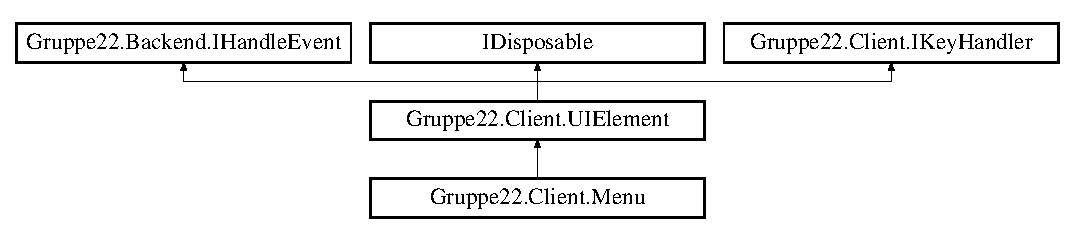
\includegraphics[height=2.692308cm]{class_gruppe22_1_1_client_1_1_menu}
\end{center}
\end{figure}
\subsection*{Öffentliche Methoden}
\begin{DoxyCompactItemize}
\item 
void \hyperlink{class_gruppe22_1_1_client_1_1_menu_ad4acef65eca04e02d56b3360b1d2692b}{Add\-Line} (string text)
\begin{DoxyCompactList}\small\item\em Append a new line of text to the list of Options \end{DoxyCompactList}\item 
override void \hyperlink{class_gruppe22_1_1_client_1_1_menu_ab51c72e83507c3eb2652456e1951acc4}{Draw} (Game\-Time game\-Time)
\begin{DoxyCompactList}\small\item\em This is called when the game should draw itself. \end{DoxyCompactList}\item 
override void \hyperlink{class_gruppe22_1_1_client_1_1_menu_a4fdd1df14f4cffa4fc2d164d9bc468f3}{Move\-Content} (Vector2 difference, int \-\_\-last\-Check=0)
\item 
override void \hyperlink{class_gruppe22_1_1_client_1_1_menu_a699aecf4ccf96cbf17a19d8c56d2cfd8}{Scroll\-Wheel} (int Difference)
\item 
\hyperlink{class_gruppe22_1_1_client_1_1_menu_ab8b07183b7dea58a5560e8b44da3e807}{Menu} (\hyperlink{interface_gruppe22_1_1_backend_1_1_i_handle_event}{Backend.\-I\-Handle\-Event} parent, Sprite\-Batch sprite\-Batch, Content\-Manager content, Rectangle display\-Rect)
\end{DoxyCompactItemize}
\subsection*{Weitere Geerbte Elemente}


\subsection{Beschreibung der Konstruktoren und Destruktoren}
\hypertarget{class_gruppe22_1_1_client_1_1_menu_ab8b07183b7dea58a5560e8b44da3e807}{\index{Gruppe22\-::\-Client\-::\-Menu@{Gruppe22\-::\-Client\-::\-Menu}!Menu@{Menu}}
\index{Menu@{Menu}!Gruppe22::Client::Menu@{Gruppe22\-::\-Client\-::\-Menu}}
\subsubsection[{Menu}]{\setlength{\rightskip}{0pt plus 5cm}Gruppe22.\-Client.\-Menu.\-Menu (
\begin{DoxyParamCaption}
\item[{{\bf Backend.\-I\-Handle\-Event}}]{parent, }
\item[{Sprite\-Batch}]{sprite\-Batch, }
\item[{Content\-Manager}]{content, }
\item[{Rectangle}]{display\-Rect}
\end{DoxyParamCaption}
)}}\label{class_gruppe22_1_1_client_1_1_menu_ab8b07183b7dea58a5560e8b44da3e807}


\subsection{Dokumentation der Elementfunktionen}
\hypertarget{class_gruppe22_1_1_client_1_1_menu_ad4acef65eca04e02d56b3360b1d2692b}{\index{Gruppe22\-::\-Client\-::\-Menu@{Gruppe22\-::\-Client\-::\-Menu}!Add\-Line@{Add\-Line}}
\index{Add\-Line@{Add\-Line}!Gruppe22::Client::Menu@{Gruppe22\-::\-Client\-::\-Menu}}
\subsubsection[{Add\-Line}]{\setlength{\rightskip}{0pt plus 5cm}void Gruppe22.\-Client.\-Menu.\-Add\-Line (
\begin{DoxyParamCaption}
\item[{string}]{text}
\end{DoxyParamCaption}
)}}\label{class_gruppe22_1_1_client_1_1_menu_ad4acef65eca04e02d56b3360b1d2692b}


Append a new line of text to the list of Options 


\begin{DoxyParams}{Parameter}
{\em text} & \\
\hline
\end{DoxyParams}
\hypertarget{class_gruppe22_1_1_client_1_1_menu_ab51c72e83507c3eb2652456e1951acc4}{\index{Gruppe22\-::\-Client\-::\-Menu@{Gruppe22\-::\-Client\-::\-Menu}!Draw@{Draw}}
\index{Draw@{Draw}!Gruppe22::Client::Menu@{Gruppe22\-::\-Client\-::\-Menu}}
\subsubsection[{Draw}]{\setlength{\rightskip}{0pt plus 5cm}override void Gruppe22.\-Client.\-Menu.\-Draw (
\begin{DoxyParamCaption}
\item[{Game\-Time}]{game\-Time}
\end{DoxyParamCaption}
)\hspace{0.3cm}{\ttfamily [virtual]}}}\label{class_gruppe22_1_1_client_1_1_menu_ab51c72e83507c3eb2652456e1951acc4}


This is called when the game should draw itself. 


\begin{DoxyParams}{Parameter}
{\em game\-Time} & Provides a snapshot of timing values.\\
\hline
\end{DoxyParams}


Erneute Implementation von \hyperlink{class_gruppe22_1_1_client_1_1_u_i_element_ae68afcbd1db3540052d6b399022e56e7}{Gruppe22.\-Client.\-U\-I\-Element}.

\hypertarget{class_gruppe22_1_1_client_1_1_menu_a4fdd1df14f4cffa4fc2d164d9bc468f3}{\index{Gruppe22\-::\-Client\-::\-Menu@{Gruppe22\-::\-Client\-::\-Menu}!Move\-Content@{Move\-Content}}
\index{Move\-Content@{Move\-Content}!Gruppe22::Client::Menu@{Gruppe22\-::\-Client\-::\-Menu}}
\subsubsection[{Move\-Content}]{\setlength{\rightskip}{0pt plus 5cm}override void Gruppe22.\-Client.\-Menu.\-Move\-Content (
\begin{DoxyParamCaption}
\item[{Vector2}]{difference, }
\item[{int}]{\-\_\-last\-Check = {\ttfamily 0}}
\end{DoxyParamCaption}
)\hspace{0.3cm}{\ttfamily [virtual]}}}\label{class_gruppe22_1_1_client_1_1_menu_a4fdd1df14f4cffa4fc2d164d9bc468f3}





\begin{DoxyParams}{Parameter}
{\em difference} & \\
\hline
\end{DoxyParams}


Erneute Implementation von \hyperlink{class_gruppe22_1_1_client_1_1_u_i_element_aa089eaf82ae3a89724a45eb8860cb97b}{Gruppe22.\-Client.\-U\-I\-Element}.

\hypertarget{class_gruppe22_1_1_client_1_1_menu_a699aecf4ccf96cbf17a19d8c56d2cfd8}{\index{Gruppe22\-::\-Client\-::\-Menu@{Gruppe22\-::\-Client\-::\-Menu}!Scroll\-Wheel@{Scroll\-Wheel}}
\index{Scroll\-Wheel@{Scroll\-Wheel}!Gruppe22::Client::Menu@{Gruppe22\-::\-Client\-::\-Menu}}
\subsubsection[{Scroll\-Wheel}]{\setlength{\rightskip}{0pt plus 5cm}override void Gruppe22.\-Client.\-Menu.\-Scroll\-Wheel (
\begin{DoxyParamCaption}
\item[{int}]{Difference}
\end{DoxyParamCaption}
)\hspace{0.3cm}{\ttfamily [virtual]}}}\label{class_gruppe22_1_1_client_1_1_menu_a699aecf4ccf96cbf17a19d8c56d2cfd8}





\begin{DoxyParams}{Parameter}
{\em Difference} & \\
\hline
\end{DoxyParams}


Erneute Implementation von \hyperlink{class_gruppe22_1_1_client_1_1_u_i_element_a691954dde0b9a1d39c064e86fea19bf5}{Gruppe22.\-Client.\-U\-I\-Element}.



Die Dokumentation für diese Klasse wurde erzeugt aufgrund der Datei\-:\begin{DoxyCompactItemize}
\item 
C\-:/\-Users/beursken/\-Documents/\-Git\-Hub/gruppe22/\-Gruppe22/\-Gruppe22/\-Client/\-U\-I/\hyperlink{_menu_8cs}{Menu.\-cs}\end{DoxyCompactItemize}

\hypertarget{class_gruppe22_1_1_client_1_1_minimap}{\section{Gruppe22.\-Client.\-Minimap Klassenreferenz}
\label{class_gruppe22_1_1_client_1_1_minimap}\index{Gruppe22.\-Client.\-Minimap@{Gruppe22.\-Client.\-Minimap}}
}
Klassendiagramm für Gruppe22.\-Client.\-Minimap\-:\begin{figure}[H]
\begin{center}
\leavevmode
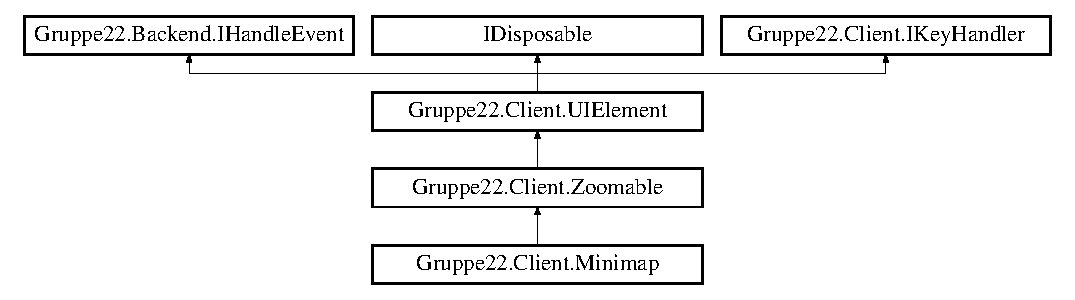
\includegraphics[height=3.589744cm]{class_gruppe22_1_1_client_1_1_minimap}
\end{center}
\end{figure}
\subsection*{Öffentliche Methoden}
\begin{DoxyCompactItemize}
\item 
override void \hyperlink{class_gruppe22_1_1_client_1_1_minimap_a32a69f8d0569dd31183d57cb04006e10}{Draw} (Game\-Time game\-Time)
\begin{DoxyCompactList}\small\item\em This is called when the game should draw itself. \end{DoxyCompactList}\item 
override void \hyperlink{class_gruppe22_1_1_client_1_1_minimap_abe87f3a3827b72df0106e5839ff9ee21}{Move\-Content} (Vector2 difference, int \-\_\-last\-Check=0)
\begin{DoxyCompactList}\small\item\em Verschiebung der gedrehten \hyperlink{class_gruppe22_1_1_client_1_1_minimap}{Minimap}. \end{DoxyCompactList}\item 
void \hyperlink{class_gruppe22_1_1_client_1_1_minimap_ad4ed9b7a0732776cbbd9a919bb087ba7}{Move\-Camera} (\hyperlink{class_gruppe22_1_1_backend_1_1_coords}{Backend.\-Coords} coords)
\item 
override void \hyperlink{class_gruppe22_1_1_client_1_1_minimap_a300b7045139787e2f35a0807793e8bc0}{Scroll\-Wheel} (int Difference)
\item 
\hyperlink{class_gruppe22_1_1_client_1_1_minimap_a23e6850c1ea74b948b47680a07749e08}{Minimap} (\hyperlink{interface_gruppe22_1_1_backend_1_1_i_handle_event}{Backend.\-I\-Handle\-Event} parent, Sprite\-Batch sprite\-Batch, Content\-Manager content, Rectangle region, \hyperlink{class_gruppe22_1_1_backend_1_1_map}{Backend.\-Map} map)
\begin{DoxyCompactList}\small\item\em Constructor \end{DoxyCompactList}\end{DoxyCompactItemize}
\subsection*{Propertys}
\begin{DoxyCompactItemize}
\item 
new float \hyperlink{class_gruppe22_1_1_client_1_1_minimap_af46608d90521f2dfb3872e996ad3ec6c}{Zoom}\hspace{0.3cm}{\ttfamily  \mbox{[}get, set\mbox{]}}
\end{DoxyCompactItemize}
\subsection*{Weitere Geerbte Elemente}


\subsection{Beschreibung der Konstruktoren und Destruktoren}
\hypertarget{class_gruppe22_1_1_client_1_1_minimap_a23e6850c1ea74b948b47680a07749e08}{\index{Gruppe22\-::\-Client\-::\-Minimap@{Gruppe22\-::\-Client\-::\-Minimap}!Minimap@{Minimap}}
\index{Minimap@{Minimap}!Gruppe22::Client::Minimap@{Gruppe22\-::\-Client\-::\-Minimap}}
\subsubsection[{Minimap}]{\setlength{\rightskip}{0pt plus 5cm}Gruppe22.\-Client.\-Minimap.\-Minimap (
\begin{DoxyParamCaption}
\item[{{\bf Backend.\-I\-Handle\-Event}}]{parent, }
\item[{Sprite\-Batch}]{sprite\-Batch, }
\item[{Content\-Manager}]{content, }
\item[{Rectangle}]{region, }
\item[{{\bf Backend.\-Map}}]{map}
\end{DoxyParamCaption}
)}}\label{class_gruppe22_1_1_client_1_1_minimap_a23e6850c1ea74b948b47680a07749e08}


Constructor 


\begin{DoxyParams}{Parameter}
{\em graphics} & \\
\hline
{\em sprite\-Batch} & \\
\hline
{\em region} & \\
\hline
{\em map\-Icons} & \\
\hline
{\em map} & \\
\hline
\end{DoxyParams}


\subsection{Dokumentation der Elementfunktionen}
\hypertarget{class_gruppe22_1_1_client_1_1_minimap_a32a69f8d0569dd31183d57cb04006e10}{\index{Gruppe22\-::\-Client\-::\-Minimap@{Gruppe22\-::\-Client\-::\-Minimap}!Draw@{Draw}}
\index{Draw@{Draw}!Gruppe22::Client::Minimap@{Gruppe22\-::\-Client\-::\-Minimap}}
\subsubsection[{Draw}]{\setlength{\rightskip}{0pt plus 5cm}override void Gruppe22.\-Client.\-Minimap.\-Draw (
\begin{DoxyParamCaption}
\item[{Game\-Time}]{game\-Time}
\end{DoxyParamCaption}
)\hspace{0.3cm}{\ttfamily [virtual]}}}\label{class_gruppe22_1_1_client_1_1_minimap_a32a69f8d0569dd31183d57cb04006e10}


This is called when the game should draw itself. 


\begin{DoxyParams}{Parameter}
{\em game\-Time} & Provides a snapshot of timing values.\\
\hline
\end{DoxyParams}


Erneute Implementation von \hyperlink{class_gruppe22_1_1_client_1_1_u_i_element_ae68afcbd1db3540052d6b399022e56e7}{Gruppe22.\-Client.\-U\-I\-Element}.

\hypertarget{class_gruppe22_1_1_client_1_1_minimap_ad4ed9b7a0732776cbbd9a919bb087ba7}{\index{Gruppe22\-::\-Client\-::\-Minimap@{Gruppe22\-::\-Client\-::\-Minimap}!Move\-Camera@{Move\-Camera}}
\index{Move\-Camera@{Move\-Camera}!Gruppe22::Client::Minimap@{Gruppe22\-::\-Client\-::\-Minimap}}
\subsubsection[{Move\-Camera}]{\setlength{\rightskip}{0pt plus 5cm}void Gruppe22.\-Client.\-Minimap.\-Move\-Camera (
\begin{DoxyParamCaption}
\item[{{\bf Backend.\-Coords}}]{coords}
\end{DoxyParamCaption}
)}}\label{class_gruppe22_1_1_client_1_1_minimap_ad4ed9b7a0732776cbbd9a919bb087ba7}
\hypertarget{class_gruppe22_1_1_client_1_1_minimap_abe87f3a3827b72df0106e5839ff9ee21}{\index{Gruppe22\-::\-Client\-::\-Minimap@{Gruppe22\-::\-Client\-::\-Minimap}!Move\-Content@{Move\-Content}}
\index{Move\-Content@{Move\-Content}!Gruppe22::Client::Minimap@{Gruppe22\-::\-Client\-::\-Minimap}}
\subsubsection[{Move\-Content}]{\setlength{\rightskip}{0pt plus 5cm}override void Gruppe22.\-Client.\-Minimap.\-Move\-Content (
\begin{DoxyParamCaption}
\item[{Vector2}]{difference, }
\item[{int}]{\-\_\-last\-Check = {\ttfamily 0}}
\end{DoxyParamCaption}
)\hspace{0.3cm}{\ttfamily [virtual]}}}\label{class_gruppe22_1_1_client_1_1_minimap_abe87f3a3827b72df0106e5839ff9ee21}


Verschiebung der gedrehten \hyperlink{class_gruppe22_1_1_client_1_1_minimap}{Minimap}. 


\begin{DoxyParams}{Parameter}
{\em difference} & \\
\hline
{\em \-\_\-last\-Check} & \\
\hline
\end{DoxyParams}


Erneute Implementation von \hyperlink{class_gruppe22_1_1_client_1_1_u_i_element_aa089eaf82ae3a89724a45eb8860cb97b}{Gruppe22.\-Client.\-U\-I\-Element}.

\hypertarget{class_gruppe22_1_1_client_1_1_minimap_a300b7045139787e2f35a0807793e8bc0}{\index{Gruppe22\-::\-Client\-::\-Minimap@{Gruppe22\-::\-Client\-::\-Minimap}!Scroll\-Wheel@{Scroll\-Wheel}}
\index{Scroll\-Wheel@{Scroll\-Wheel}!Gruppe22::Client::Minimap@{Gruppe22\-::\-Client\-::\-Minimap}}
\subsubsection[{Scroll\-Wheel}]{\setlength{\rightskip}{0pt plus 5cm}override void Gruppe22.\-Client.\-Minimap.\-Scroll\-Wheel (
\begin{DoxyParamCaption}
\item[{int}]{Difference}
\end{DoxyParamCaption}
)\hspace{0.3cm}{\ttfamily [virtual]}}}\label{class_gruppe22_1_1_client_1_1_minimap_a300b7045139787e2f35a0807793e8bc0}





\begin{DoxyParams}{Parameter}
{\em Difference} & \\
\hline
\end{DoxyParams}


Erneute Implementation von \hyperlink{class_gruppe22_1_1_client_1_1_u_i_element_a691954dde0b9a1d39c064e86fea19bf5}{Gruppe22.\-Client.\-U\-I\-Element}.



\subsection{Dokumentation der Propertys}
\hypertarget{class_gruppe22_1_1_client_1_1_minimap_af46608d90521f2dfb3872e996ad3ec6c}{\index{Gruppe22\-::\-Client\-::\-Minimap@{Gruppe22\-::\-Client\-::\-Minimap}!Zoom@{Zoom}}
\index{Zoom@{Zoom}!Gruppe22::Client::Minimap@{Gruppe22\-::\-Client\-::\-Minimap}}
\subsubsection[{Zoom}]{\setlength{\rightskip}{0pt plus 5cm}new float Gruppe22.\-Client.\-Minimap.\-Zoom\hspace{0.3cm}{\ttfamily [get]}, {\ttfamily [set]}}}\label{class_gruppe22_1_1_client_1_1_minimap_af46608d90521f2dfb3872e996ad3ec6c}


Die Dokumentation für diese Klasse wurde erzeugt aufgrund der Datei\-:\begin{DoxyCompactItemize}
\item 
C\-:/\-Users/beursken/\-Documents/\-Git\-Hub/gruppe22/\-Gruppe22/\-Gruppe22/\-Client/\-Map/\hyperlink{_minimap_8cs}{Minimap.\-cs}\end{DoxyCompactItemize}

\hypertarget{class_gruppe22_1_1_client_1_1_modify_window}{\section{Gruppe22.\-Client.\-Modify\-Window Klassenreferenz}
\label{class_gruppe22_1_1_client_1_1_modify_window}\index{Gruppe22.\-Client.\-Modify\-Window@{Gruppe22.\-Client.\-Modify\-Window}}
}
Klassendiagramm für Gruppe22.\-Client.\-Modify\-Window\-:\begin{figure}[H]
\begin{center}
\leavevmode
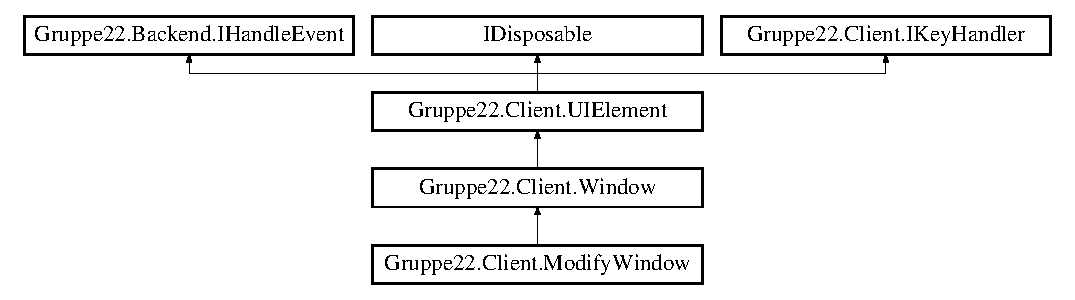
\includegraphics[height=3.589744cm]{class_gruppe22_1_1_client_1_1_modify_window}
\end{center}
\end{figure}
\subsection*{Öffentliche Methoden}
\begin{DoxyCompactItemize}
\item 
\hyperlink{class_gruppe22_1_1_client_1_1_modify_window_a2ff4c3551990556ce8a2fd1ceb97f04f}{Modify\-Window} (\hyperlink{interface_gruppe22_1_1_backend_1_1_i_handle_event}{Backend.\-I\-Handle\-Event} parent, Sprite\-Batch sprite\-Batch, Content\-Manager content, Rectangle display\-Rect, \hyperlink{class_gruppe22_1_1_backend_1_1_item}{Backend.\-Item} item)
\begin{DoxyCompactList}\small\item\em Constructor \end{DoxyCompactList}\end{DoxyCompactItemize}
\subsection*{Weitere Geerbte Elemente}


\subsection{Beschreibung der Konstruktoren und Destruktoren}
\hypertarget{class_gruppe22_1_1_client_1_1_modify_window_a2ff4c3551990556ce8a2fd1ceb97f04f}{\index{Gruppe22\-::\-Client\-::\-Modify\-Window@{Gruppe22\-::\-Client\-::\-Modify\-Window}!Modify\-Window@{Modify\-Window}}
\index{Modify\-Window@{Modify\-Window}!Gruppe22::Client::ModifyWindow@{Gruppe22\-::\-Client\-::\-Modify\-Window}}
\subsubsection[{Modify\-Window}]{\setlength{\rightskip}{0pt plus 5cm}Gruppe22.\-Client.\-Modify\-Window.\-Modify\-Window (
\begin{DoxyParamCaption}
\item[{{\bf Backend.\-I\-Handle\-Event}}]{parent, }
\item[{Sprite\-Batch}]{sprite\-Batch, }
\item[{Content\-Manager}]{content, }
\item[{Rectangle}]{display\-Rect, }
\item[{{\bf Backend.\-Item}}]{item}
\end{DoxyParamCaption}
)}}\label{class_gruppe22_1_1_client_1_1_modify_window_a2ff4c3551990556ce8a2fd1ceb97f04f}


Constructor 



Die Dokumentation für diese Klasse wurde erzeugt aufgrund der Datei\-:\begin{DoxyCompactItemize}
\item 
C\-:/\-Users/beursken/\-Documents/\-Git\-Hub/gruppe22/\-Gruppe22/\-Gruppe22/\-Client/\-U\-I/\hyperlink{_modify_window_8cs}{Modify\-Window.\-cs}\end{DoxyCompactItemize}

\hypertarget{class_gruppe22_1_1_backend_1_1_movable_tile}{\section{Gruppe22.\-Backend.\-Movable\-Tile Klassenreferenz}
\label{class_gruppe22_1_1_backend_1_1_movable_tile}\index{Gruppe22.\-Backend.\-Movable\-Tile@{Gruppe22.\-Backend.\-Movable\-Tile}}
}


Die Dokumentation für diese Klasse wurde erzeugt aufgrund der Datei\-:\begin{DoxyCompactItemize}
\item 
C\-:/\-Users/beursken/\-Documents/\-Git\-Hub/gruppe22/\-Gruppe22/\-Gruppe22/\-Backend/\-Map/\hyperlink{_movable_tile_8cs}{Movable\-Tile.\-cs}\end{DoxyCompactItemize}

\hypertarget{class_gruppe22_1_1_client_1_1_net_player}{\section{Gruppe22.\-Client.\-Net\-Player Klassenreferenz}
\label{class_gruppe22_1_1_client_1_1_net_player}\index{Gruppe22.\-Client.\-Net\-Player@{Gruppe22.\-Client.\-Net\-Player}}
}
\subsection*{Öffentliche Methoden}
\begin{DoxyCompactItemize}
\item 
void \hyperlink{class_gruppe22_1_1_client_1_1_net_player_ab69004f431aba560132757ddc248f10d}{Start} ()
\item 
void \hyperlink{class_gruppe22_1_1_client_1_1_net_player_a988e77763c29eccac9d19b17b6650436}{Stop} ()
\item 
void \hyperlink{class_gruppe22_1_1_client_1_1_net_player_ae8f57a7ea6a2aeca629262d7df3a2981}{Update} (Game\-Time game\-Time)
\item 
void \hyperlink{class_gruppe22_1_1_client_1_1_net_player_a2afed4682416d522e896f3e45209e018}{Do\-Move} (int Char\-I\-D, \hyperlink{namespace_gruppe22_1_1_backend_a2d53d5d14b8ea0951ba6971e5da1ebf5}{Backend.\-Direction} dir, \hyperlink{class_gruppe22_1_1_backend_1_1_coords}{Backend.\-Coords} pos)
\item 
\hyperlink{class_gruppe22_1_1_client_1_1_net_player_a9828b0f862a08d56593722849e0dc200}{Net\-Player} (\hyperlink{interface_gruppe22_1_1_backend_1_1_i_handle_event}{Backend.\-I\-Handle\-Event} parent)
\end{DoxyCompactItemize}
\subsection*{Öffentliche Attribute}
\begin{DoxyCompactItemize}
\item 
Dictionary$<$ string, string $>$ \hyperlink{class_gruppe22_1_1_client_1_1_net_player_a9dc0068c252f2e59928f77ae43e76aa1}{\-\_\-servers}
\end{DoxyCompactItemize}
\subsection*{Propertys}
\begin{DoxyCompactItemize}
\item 
string \hyperlink{class_gruppe22_1_1_client_1_1_net_player_a7b62a0490b4c13e5f6c1e2dad62a1916}{server}\hspace{0.3cm}{\ttfamily  \mbox{[}get, set\mbox{]}}
\item 
string \hyperlink{class_gruppe22_1_1_client_1_1_net_player_ad1a5e262126571468b615e44674d8be1}{playername}\hspace{0.3cm}{\ttfamily  \mbox{[}get, set\mbox{]}}
\end{DoxyCompactItemize}


\subsection{Beschreibung der Konstruktoren und Destruktoren}
\hypertarget{class_gruppe22_1_1_client_1_1_net_player_a9828b0f862a08d56593722849e0dc200}{\index{Gruppe22\-::\-Client\-::\-Net\-Player@{Gruppe22\-::\-Client\-::\-Net\-Player}!Net\-Player@{Net\-Player}}
\index{Net\-Player@{Net\-Player}!Gruppe22::Client::NetPlayer@{Gruppe22\-::\-Client\-::\-Net\-Player}}
\subsubsection[{Net\-Player}]{\setlength{\rightskip}{0pt plus 5cm}Gruppe22.\-Client.\-Net\-Player.\-Net\-Player (
\begin{DoxyParamCaption}
\item[{{\bf Backend.\-I\-Handle\-Event}}]{parent}
\end{DoxyParamCaption}
)}}\label{class_gruppe22_1_1_client_1_1_net_player_a9828b0f862a08d56593722849e0dc200}


\subsection{Dokumentation der Elementfunktionen}
\hypertarget{class_gruppe22_1_1_client_1_1_net_player_a2afed4682416d522e896f3e45209e018}{\index{Gruppe22\-::\-Client\-::\-Net\-Player@{Gruppe22\-::\-Client\-::\-Net\-Player}!Do\-Move@{Do\-Move}}
\index{Do\-Move@{Do\-Move}!Gruppe22::Client::NetPlayer@{Gruppe22\-::\-Client\-::\-Net\-Player}}
\subsubsection[{Do\-Move}]{\setlength{\rightskip}{0pt plus 5cm}void Gruppe22.\-Client.\-Net\-Player.\-Do\-Move (
\begin{DoxyParamCaption}
\item[{int}]{Char\-I\-D, }
\item[{{\bf Backend.\-Direction}}]{dir, }
\item[{{\bf Backend.\-Coords}}]{pos}
\end{DoxyParamCaption}
)}}\label{class_gruppe22_1_1_client_1_1_net_player_a2afed4682416d522e896f3e45209e018}
\hypertarget{class_gruppe22_1_1_client_1_1_net_player_ab69004f431aba560132757ddc248f10d}{\index{Gruppe22\-::\-Client\-::\-Net\-Player@{Gruppe22\-::\-Client\-::\-Net\-Player}!Start@{Start}}
\index{Start@{Start}!Gruppe22::Client::NetPlayer@{Gruppe22\-::\-Client\-::\-Net\-Player}}
\subsubsection[{Start}]{\setlength{\rightskip}{0pt plus 5cm}void Gruppe22.\-Client.\-Net\-Player.\-Start (
\begin{DoxyParamCaption}
{}
\end{DoxyParamCaption}
)}}\label{class_gruppe22_1_1_client_1_1_net_player_ab69004f431aba560132757ddc248f10d}
\hypertarget{class_gruppe22_1_1_client_1_1_net_player_a988e77763c29eccac9d19b17b6650436}{\index{Gruppe22\-::\-Client\-::\-Net\-Player@{Gruppe22\-::\-Client\-::\-Net\-Player}!Stop@{Stop}}
\index{Stop@{Stop}!Gruppe22::Client::NetPlayer@{Gruppe22\-::\-Client\-::\-Net\-Player}}
\subsubsection[{Stop}]{\setlength{\rightskip}{0pt plus 5cm}void Gruppe22.\-Client.\-Net\-Player.\-Stop (
\begin{DoxyParamCaption}
{}
\end{DoxyParamCaption}
)}}\label{class_gruppe22_1_1_client_1_1_net_player_a988e77763c29eccac9d19b17b6650436}
\hypertarget{class_gruppe22_1_1_client_1_1_net_player_ae8f57a7ea6a2aeca629262d7df3a2981}{\index{Gruppe22\-::\-Client\-::\-Net\-Player@{Gruppe22\-::\-Client\-::\-Net\-Player}!Update@{Update}}
\index{Update@{Update}!Gruppe22::Client::NetPlayer@{Gruppe22\-::\-Client\-::\-Net\-Player}}
\subsubsection[{Update}]{\setlength{\rightskip}{0pt plus 5cm}void Gruppe22.\-Client.\-Net\-Player.\-Update (
\begin{DoxyParamCaption}
\item[{Game\-Time}]{game\-Time}
\end{DoxyParamCaption}
)}}\label{class_gruppe22_1_1_client_1_1_net_player_ae8f57a7ea6a2aeca629262d7df3a2981}


\subsection{Dokumentation der Datenelemente}
\hypertarget{class_gruppe22_1_1_client_1_1_net_player_a9dc0068c252f2e59928f77ae43e76aa1}{\index{Gruppe22\-::\-Client\-::\-Net\-Player@{Gruppe22\-::\-Client\-::\-Net\-Player}!\-\_\-servers@{\-\_\-servers}}
\index{\-\_\-servers@{\-\_\-servers}!Gruppe22::Client::NetPlayer@{Gruppe22\-::\-Client\-::\-Net\-Player}}
\subsubsection[{\-\_\-servers}]{\setlength{\rightskip}{0pt plus 5cm}Dictionary$<$string, string$>$ Gruppe22.\-Client.\-Net\-Player.\-\_\-servers}}\label{class_gruppe22_1_1_client_1_1_net_player_a9dc0068c252f2e59928f77ae43e76aa1}


\subsection{Dokumentation der Propertys}
\hypertarget{class_gruppe22_1_1_client_1_1_net_player_ad1a5e262126571468b615e44674d8be1}{\index{Gruppe22\-::\-Client\-::\-Net\-Player@{Gruppe22\-::\-Client\-::\-Net\-Player}!playername@{playername}}
\index{playername@{playername}!Gruppe22::Client::NetPlayer@{Gruppe22\-::\-Client\-::\-Net\-Player}}
\subsubsection[{playername}]{\setlength{\rightskip}{0pt plus 5cm}string Gruppe22.\-Client.\-Net\-Player.\-playername\hspace{0.3cm}{\ttfamily [get]}, {\ttfamily [set]}}}\label{class_gruppe22_1_1_client_1_1_net_player_ad1a5e262126571468b615e44674d8be1}
\hypertarget{class_gruppe22_1_1_client_1_1_net_player_a7b62a0490b4c13e5f6c1e2dad62a1916}{\index{Gruppe22\-::\-Client\-::\-Net\-Player@{Gruppe22\-::\-Client\-::\-Net\-Player}!server@{server}}
\index{server@{server}!Gruppe22::Client::NetPlayer@{Gruppe22\-::\-Client\-::\-Net\-Player}}
\subsubsection[{server}]{\setlength{\rightskip}{0pt plus 5cm}string Gruppe22.\-Client.\-Net\-Player.\-server\hspace{0.3cm}{\ttfamily [get]}, {\ttfamily [set]}}}\label{class_gruppe22_1_1_client_1_1_net_player_a7b62a0490b4c13e5f6c1e2dad62a1916}


Die Dokumentation für diese Klasse wurde erzeugt aufgrund der Datei\-:\begin{DoxyCompactItemize}
\item 
C\-:/\-Users/beursken/\-Documents/\-Git\-Hub/gruppe22/\-Gruppe22/\-Gruppe22/\-Client/\-Network/\hyperlink{_net_player_8cs}{Net\-Player.\-cs}\end{DoxyCompactItemize}

\hypertarget{class_gruppe22_1_1_backend_1_1_n_p_c}{\section{Gruppe22.\-Backend.\-N\-P\-C Klassenreferenz}
\label{class_gruppe22_1_1_backend_1_1_n_p_c}\index{Gruppe22.\-Backend.\-N\-P\-C@{Gruppe22.\-Backend.\-N\-P\-C}}
}
Klassendiagramm für Gruppe22.\-Backend.\-N\-P\-C\-:\begin{figure}[H]
\begin{center}
\leavevmode
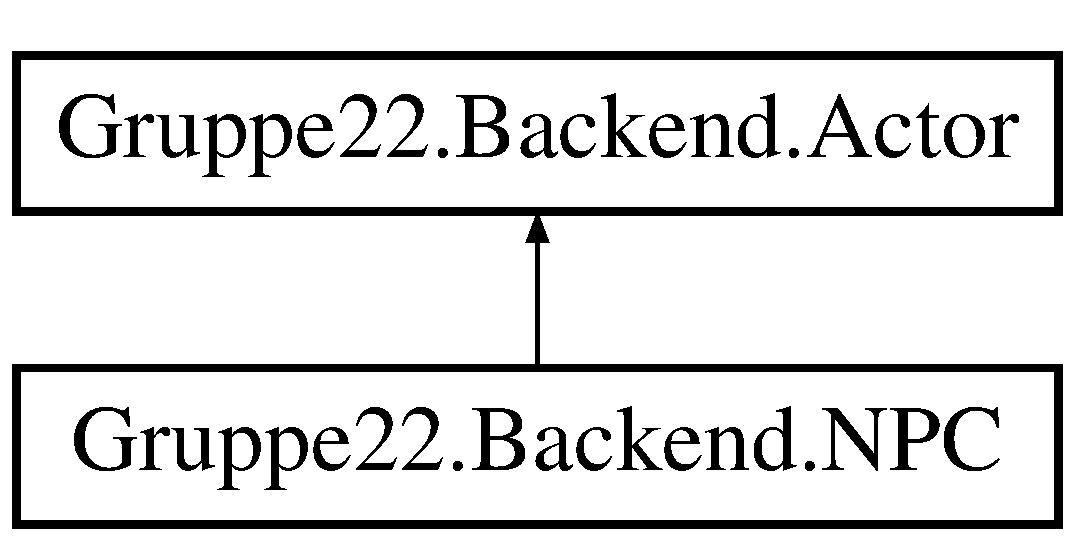
\includegraphics[height=2.000000cm]{class_gruppe22_1_1_backend_1_1_n_p_c}
\end{center}
\end{figure}
\subsection*{Öffentliche Methoden}
\begin{DoxyCompactItemize}
\item 
void \hyperlink{class_gruppe22_1_1_backend_1_1_n_p_c_a8d78d66f0c812fa44a654688433d7db5}{Interact} ()
\begin{DoxyCompactList}\small\item\em Interaktion des \hyperlink{class_gruppe22_1_1_backend_1_1_n_p_c}{N\-P\-C}. Aktion öffne Schop bzw. Dialog. Funktionsweise uber Eventaufruf. \end{DoxyCompactList}\item 
\hyperlink{class_gruppe22_1_1_backend_1_1_n_p_c_ad228f41a3a754678a2f700455fec4db8}{N\-P\-C} (Content\-Manager content, int \hyperlink{class_gruppe22_1_1_backend_1_1_actor_a46f3a7d62de83a6bf3c44cd52f38af9b}{health}=10, int \hyperlink{class_gruppe22_1_1_backend_1_1_actor_ab400f0b82f96d2334891d7cd428f5d08}{armor}=0, int \hyperlink{class_gruppe22_1_1_backend_1_1_actor_a461e2480a59de23517c3b375dede10fb}{damage}=0, int \hyperlink{class_gruppe22_1_1_backend_1_1_actor_aac0f2f9a2f0b314f98ba19d0b38a7a97}{max\-Health}=10, string \hyperlink{class_gruppe22_1_1_backend_1_1_actor_a28129eaf9d70d9bfc33a29544ba74edf}{name}=\char`\"{}\char`\"{}, Random r=null, int \hyperlink{class_gruppe22_1_1_backend_1_1_actor_ace31c72a0fd9bb941df7112647dff86d}{\-\_\-level}=1, bool shop=false)
\begin{DoxyCompactList}\small\item\em Konstruktor. Initiallisierung der Grafikverweise. \end{DoxyCompactList}\end{DoxyCompactItemize}
\subsection*{Propertys}
\begin{DoxyCompactItemize}
\item 
bool \hyperlink{class_gruppe22_1_1_backend_1_1_n_p_c_a0193fbcb07006b019c6065f5141c9da4}{has\-Shop}\hspace{0.3cm}{\ttfamily  \mbox{[}get, set\mbox{]}}
\begin{DoxyCompactList}\small\item\em Öffentliche Eigenschaft zu \-\_\-has\-Shop. \end{DoxyCompactList}\item 
bool \hyperlink{class_gruppe22_1_1_backend_1_1_n_p_c_aef91a83236e696ba3707b3514baef884}{has\-Dialogue}\hspace{0.3cm}{\ttfamily  \mbox{[}get, set\mbox{]}}
\begin{DoxyCompactList}\small\item\em Öffentliche Eigenschaft zu \-\_\-has\-Dialogue. \end{DoxyCompactList}\item 
int \hyperlink{class_gruppe22_1_1_backend_1_1_n_p_c_a6bdbcf8d62b4bc5605e7949012197908}{love}\hspace{0.3cm}{\ttfamily  \mbox{[}get, set\mbox{]}}
\begin{DoxyCompactList}\small\item\em Öffentlcie Eigenschaft zu \-\_\-love. \end{DoxyCompactList}\end{DoxyCompactItemize}
\subsection*{Weitere Geerbte Elemente}


\subsection{Beschreibung der Konstruktoren und Destruktoren}
\hypertarget{class_gruppe22_1_1_backend_1_1_n_p_c_ad228f41a3a754678a2f700455fec4db8}{\index{Gruppe22\-::\-Backend\-::\-N\-P\-C@{Gruppe22\-::\-Backend\-::\-N\-P\-C}!N\-P\-C@{N\-P\-C}}
\index{N\-P\-C@{N\-P\-C}!Gruppe22::Backend::NPC@{Gruppe22\-::\-Backend\-::\-N\-P\-C}}
\subsubsection[{N\-P\-C}]{\setlength{\rightskip}{0pt plus 5cm}Gruppe22.\-Backend.\-N\-P\-C.\-N\-P\-C (
\begin{DoxyParamCaption}
\item[{Content\-Manager}]{content, }
\item[{int}]{health = {\ttfamily 10}, }
\item[{int}]{armor = {\ttfamily 0}, }
\item[{int}]{damage = {\ttfamily 0}, }
\item[{int}]{max\-Health = {\ttfamily 10}, }
\item[{string}]{name = {\ttfamily \char`\"{}\char`\"{}}, }
\item[{Random}]{r = {\ttfamily null}, }
\item[{int}]{\-\_\-level = {\ttfamily 1}, }
\item[{bool}]{shop = {\ttfamily false}}
\end{DoxyParamCaption}
)}}\label{class_gruppe22_1_1_backend_1_1_n_p_c_ad228f41a3a754678a2f700455fec4db8}


Konstruktor. Initiallisierung der Grafikverweise. 


\begin{DoxyParams}{Parameter}
{\em content} & Resoursenverwaltung.\\
\hline
{\em health} & Lebenspunkte, Standardwert ist 10.\\
\hline
{\em armor} & Rüstung, Standardwert ist 0.\\
\hline
{\em damage} & Schaden, Standardwert ist 0.\\
\hline
{\em max\-Health} & Maximale Lebenspunkte, Standardwert ist 10.\\
\hline
{\em name} & Name des N\-P\-Cs.\\
\hline
{\em r} & Randomobjekt für die Basisklasse.\\
\hline
{\em \-\_\-level} & \hyperlink{class_gruppe22_1_1_backend_1_1_n_p_c}{N\-P\-C} aus dem Level \-\_\-level.\\
\hline
{\em shop} & Legt fest ob der \hyperlink{class_gruppe22_1_1_backend_1_1_n_p_c}{N\-P\-C} ein Shop ist.\\
\hline
\end{DoxyParams}


\subsection{Dokumentation der Elementfunktionen}
\hypertarget{class_gruppe22_1_1_backend_1_1_n_p_c_a8d78d66f0c812fa44a654688433d7db5}{\index{Gruppe22\-::\-Backend\-::\-N\-P\-C@{Gruppe22\-::\-Backend\-::\-N\-P\-C}!Interact@{Interact}}
\index{Interact@{Interact}!Gruppe22::Backend::NPC@{Gruppe22\-::\-Backend\-::\-N\-P\-C}}
\subsubsection[{Interact}]{\setlength{\rightskip}{0pt plus 5cm}void Gruppe22.\-Backend.\-N\-P\-C.\-Interact (
\begin{DoxyParamCaption}
{}
\end{DoxyParamCaption}
)}}\label{class_gruppe22_1_1_backend_1_1_n_p_c_a8d78d66f0c812fa44a654688433d7db5}


Interaktion des \hyperlink{class_gruppe22_1_1_backend_1_1_n_p_c}{N\-P\-C}. Aktion öffne Schop bzw. Dialog. Funktionsweise uber Eventaufruf. 



\subsection{Dokumentation der Propertys}
\hypertarget{class_gruppe22_1_1_backend_1_1_n_p_c_aef91a83236e696ba3707b3514baef884}{\index{Gruppe22\-::\-Backend\-::\-N\-P\-C@{Gruppe22\-::\-Backend\-::\-N\-P\-C}!has\-Dialogue@{has\-Dialogue}}
\index{has\-Dialogue@{has\-Dialogue}!Gruppe22::Backend::NPC@{Gruppe22\-::\-Backend\-::\-N\-P\-C}}
\subsubsection[{has\-Dialogue}]{\setlength{\rightskip}{0pt plus 5cm}bool Gruppe22.\-Backend.\-N\-P\-C.\-has\-Dialogue\hspace{0.3cm}{\ttfamily [get]}, {\ttfamily [set]}}}\label{class_gruppe22_1_1_backend_1_1_n_p_c_aef91a83236e696ba3707b3514baef884}


Öffentliche Eigenschaft zu \-\_\-has\-Dialogue. 

\hypertarget{class_gruppe22_1_1_backend_1_1_n_p_c_a0193fbcb07006b019c6065f5141c9da4}{\index{Gruppe22\-::\-Backend\-::\-N\-P\-C@{Gruppe22\-::\-Backend\-::\-N\-P\-C}!has\-Shop@{has\-Shop}}
\index{has\-Shop@{has\-Shop}!Gruppe22::Backend::NPC@{Gruppe22\-::\-Backend\-::\-N\-P\-C}}
\subsubsection[{has\-Shop}]{\setlength{\rightskip}{0pt plus 5cm}bool Gruppe22.\-Backend.\-N\-P\-C.\-has\-Shop\hspace{0.3cm}{\ttfamily [get]}, {\ttfamily [set]}}}\label{class_gruppe22_1_1_backend_1_1_n_p_c_a0193fbcb07006b019c6065f5141c9da4}


Öffentliche Eigenschaft zu \-\_\-has\-Shop. 

\hypertarget{class_gruppe22_1_1_backend_1_1_n_p_c_a6bdbcf8d62b4bc5605e7949012197908}{\index{Gruppe22\-::\-Backend\-::\-N\-P\-C@{Gruppe22\-::\-Backend\-::\-N\-P\-C}!love@{love}}
\index{love@{love}!Gruppe22::Backend::NPC@{Gruppe22\-::\-Backend\-::\-N\-P\-C}}
\subsubsection[{love}]{\setlength{\rightskip}{0pt plus 5cm}int Gruppe22.\-Backend.\-N\-P\-C.\-love\hspace{0.3cm}{\ttfamily [get]}, {\ttfamily [set]}}}\label{class_gruppe22_1_1_backend_1_1_n_p_c_a6bdbcf8d62b4bc5605e7949012197908}


Öffentlcie Eigenschaft zu \-\_\-love. 



Die Dokumentation für diese Klasse wurde erzeugt aufgrund der Datei\-:\begin{DoxyCompactItemize}
\item 
C\-:/\-Users/beursken/\-Documents/\-Git\-Hub/gruppe22/\-Gruppe22/\-Gruppe22/\-Backend/\-Actors/\hyperlink{_n_p_c_8cs}{N\-P\-C.\-cs}\end{DoxyCompactItemize}

\hypertarget{class_gruppe22_1_1_client_1_1_number_entry}{\section{Gruppe22.\-Client.\-Number\-Entry Klassenreferenz}
\label{class_gruppe22_1_1_client_1_1_number_entry}\index{Gruppe22.\-Client.\-Number\-Entry@{Gruppe22.\-Client.\-Number\-Entry}}
}
Klassendiagramm für Gruppe22.\-Client.\-Number\-Entry\-:\begin{figure}[H]
\begin{center}
\leavevmode
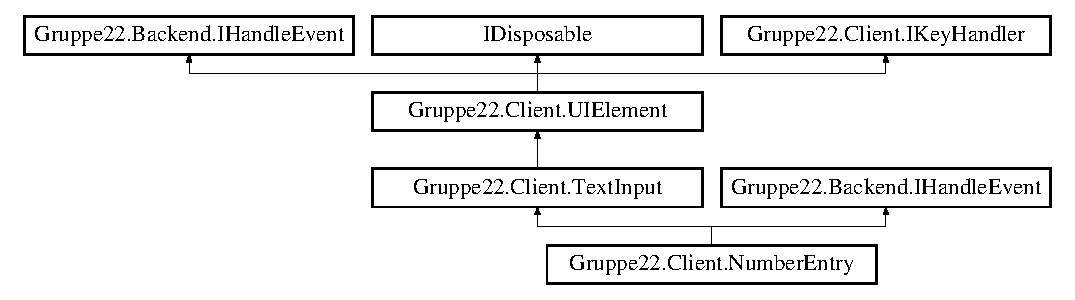
\includegraphics[height=3.589744cm]{class_gruppe22_1_1_client_1_1_number_entry}
\end{center}
\end{figure}
\subsection*{Öffentliche Methoden}
\begin{DoxyCompactItemize}
\item 
override bool \hyperlink{class_gruppe22_1_1_client_1_1_number_entry_aa343011468244db0c7630ac020a701f5}{On\-Key\-Down} (Microsoft.\-Xna.\-Framework.\-Input.\-Keys k)
\item 
override bool \hyperlink{class_gruppe22_1_1_client_1_1_number_entry_afe70d1af7d72762dc877ead2de4489f6}{On\-Mouse\-Down} (int button)
\begin{DoxyCompactList}\small\item\em Called when a mouse button changes from up to down \end{DoxyCompactList}\item 
override void \hyperlink{class_gruppe22_1_1_client_1_1_number_entry_ad662c3ad36f43640e8c662fcc3223f74}{Draw} (Game\-Time game\-Time)
\item 
\hyperlink{class_gruppe22_1_1_client_1_1_number_entry_a1fc8e5ee8a323496a1ae837479da5254}{Number\-Entry} (\hyperlink{interface_gruppe22_1_1_backend_1_1_i_handle_event}{Backend.\-I\-Handle\-Event} parent, Sprite\-Batch sprite\-Batch, Content\-Manager content, Rectangle display\-Rect, string label, int \hyperlink{class_gruppe22_1_1_client_1_1_number_entry_a3164c478660266404474cd85491db5dc}{value}, string tool\-Tip, int input\-Width, bool \hyperlink{class_gruppe22_1_1_client_1_1_text_input_ae512171e8f7caead8c28eb9327ccbf40}{can\-Edit})
\end{DoxyCompactItemize}
\subsection*{Propertys}
\begin{DoxyCompactItemize}
\item 
int \hyperlink{class_gruppe22_1_1_client_1_1_number_entry_a3164c478660266404474cd85491db5dc}{value}\hspace{0.3cm}{\ttfamily  \mbox{[}get, set\mbox{]}}
\item 
bool \hyperlink{class_gruppe22_1_1_client_1_1_number_entry_ab2e9964f2a930a81153ba75e29c0e516}{allow\-Increase}\hspace{0.3cm}{\ttfamily  \mbox{[}get, set\mbox{]}}
\item 
int \hyperlink{class_gruppe22_1_1_client_1_1_number_entry_a90ab861f29fca9349151bfd7d25b2864}{original\-Value}\hspace{0.3cm}{\ttfamily  \mbox{[}get\mbox{]}}
\item 
bool \hyperlink{class_gruppe22_1_1_client_1_1_number_entry_a8805cd126c619a1e1d412186db7566e9}{allow\-Decrease}\hspace{0.3cm}{\ttfamily  \mbox{[}get, set\mbox{]}}
\item 
override bool \hyperlink{class_gruppe22_1_1_client_1_1_number_entry_ac2d593413d374a96922404868e37be47}{can\-Focus}\hspace{0.3cm}{\ttfamily  \mbox{[}get\mbox{]}}
\end{DoxyCompactItemize}
\subsection*{Weitere Geerbte Elemente}


\subsection{Beschreibung der Konstruktoren und Destruktoren}
\hypertarget{class_gruppe22_1_1_client_1_1_number_entry_a1fc8e5ee8a323496a1ae837479da5254}{\index{Gruppe22\-::\-Client\-::\-Number\-Entry@{Gruppe22\-::\-Client\-::\-Number\-Entry}!Number\-Entry@{Number\-Entry}}
\index{Number\-Entry@{Number\-Entry}!Gruppe22::Client::NumberEntry@{Gruppe22\-::\-Client\-::\-Number\-Entry}}
\subsubsection[{Number\-Entry}]{\setlength{\rightskip}{0pt plus 5cm}Gruppe22.\-Client.\-Number\-Entry.\-Number\-Entry (
\begin{DoxyParamCaption}
\item[{{\bf Backend.\-I\-Handle\-Event}}]{parent, }
\item[{Sprite\-Batch}]{sprite\-Batch, }
\item[{Content\-Manager}]{content, }
\item[{Rectangle}]{display\-Rect, }
\item[{string}]{label, }
\item[{int}]{value, }
\item[{string}]{tool\-Tip, }
\item[{int}]{input\-Width, }
\item[{bool}]{can\-Edit}
\end{DoxyParamCaption}
)}}\label{class_gruppe22_1_1_client_1_1_number_entry_a1fc8e5ee8a323496a1ae837479da5254}





\begin{DoxyParams}{Parameter}
{\em sprite\-Batch} & \\
\hline
{\em content} & \\
\hline
{\em display\-Rect} & \\
\hline
\end{DoxyParams}


\subsection{Dokumentation der Elementfunktionen}
\hypertarget{class_gruppe22_1_1_client_1_1_number_entry_ad662c3ad36f43640e8c662fcc3223f74}{\index{Gruppe22\-::\-Client\-::\-Number\-Entry@{Gruppe22\-::\-Client\-::\-Number\-Entry}!Draw@{Draw}}
\index{Draw@{Draw}!Gruppe22::Client::NumberEntry@{Gruppe22\-::\-Client\-::\-Number\-Entry}}
\subsubsection[{Draw}]{\setlength{\rightskip}{0pt plus 5cm}override void Gruppe22.\-Client.\-Number\-Entry.\-Draw (
\begin{DoxyParamCaption}
\item[{Game\-Time}]{game\-Time}
\end{DoxyParamCaption}
)\hspace{0.3cm}{\ttfamily [virtual]}}}\label{class_gruppe22_1_1_client_1_1_number_entry_ad662c3ad36f43640e8c662fcc3223f74}





\begin{DoxyParams}{Parameter}
{\em game\-Time} & \\
\hline
\end{DoxyParams}


Erneute Implementation von \hyperlink{class_gruppe22_1_1_client_1_1_u_i_element_ae68afcbd1db3540052d6b399022e56e7}{Gruppe22.\-Client.\-U\-I\-Element}.

\hypertarget{class_gruppe22_1_1_client_1_1_number_entry_aa343011468244db0c7630ac020a701f5}{\index{Gruppe22\-::\-Client\-::\-Number\-Entry@{Gruppe22\-::\-Client\-::\-Number\-Entry}!On\-Key\-Down@{On\-Key\-Down}}
\index{On\-Key\-Down@{On\-Key\-Down}!Gruppe22::Client::NumberEntry@{Gruppe22\-::\-Client\-::\-Number\-Entry}}
\subsubsection[{On\-Key\-Down}]{\setlength{\rightskip}{0pt plus 5cm}override bool Gruppe22.\-Client.\-Number\-Entry.\-On\-Key\-Down (
\begin{DoxyParamCaption}
\item[{Microsoft.\-Xna.\-Framework.\-Input.\-Keys}]{k}
\end{DoxyParamCaption}
)}}\label{class_gruppe22_1_1_client_1_1_number_entry_aa343011468244db0c7630ac020a701f5}
\hypertarget{class_gruppe22_1_1_client_1_1_number_entry_afe70d1af7d72762dc877ead2de4489f6}{\index{Gruppe22\-::\-Client\-::\-Number\-Entry@{Gruppe22\-::\-Client\-::\-Number\-Entry}!On\-Mouse\-Down@{On\-Mouse\-Down}}
\index{On\-Mouse\-Down@{On\-Mouse\-Down}!Gruppe22::Client::NumberEntry@{Gruppe22\-::\-Client\-::\-Number\-Entry}}
\subsubsection[{On\-Mouse\-Down}]{\setlength{\rightskip}{0pt plus 5cm}override bool Gruppe22.\-Client.\-Number\-Entry.\-On\-Mouse\-Down (
\begin{DoxyParamCaption}
\item[{int}]{button}
\end{DoxyParamCaption}
)\hspace{0.3cm}{\ttfamily [virtual]}}}\label{class_gruppe22_1_1_client_1_1_number_entry_afe70d1af7d72762dc877ead2de4489f6}


Called when a mouse button changes from up to down 


\begin{DoxyParams}{Parameter}
{\em button} & Left \hyperlink{class_gruppe22_1_1_client_1_1_button}{Button}=1, Middle \hyperlink{class_gruppe22_1_1_client_1_1_button}{Button}=2, Right \hyperlink{class_gruppe22_1_1_client_1_1_button}{Button}=3\\
\hline
\end{DoxyParams}


Erneute Implementation von \hyperlink{class_gruppe22_1_1_client_1_1_u_i_element_a0530df2286336160b8b39c74ba380a44}{Gruppe22.\-Client.\-U\-I\-Element}.



\subsection{Dokumentation der Propertys}
\hypertarget{class_gruppe22_1_1_client_1_1_number_entry_a8805cd126c619a1e1d412186db7566e9}{\index{Gruppe22\-::\-Client\-::\-Number\-Entry@{Gruppe22\-::\-Client\-::\-Number\-Entry}!allow\-Decrease@{allow\-Decrease}}
\index{allow\-Decrease@{allow\-Decrease}!Gruppe22::Client::NumberEntry@{Gruppe22\-::\-Client\-::\-Number\-Entry}}
\subsubsection[{allow\-Decrease}]{\setlength{\rightskip}{0pt plus 5cm}bool Gruppe22.\-Client.\-Number\-Entry.\-allow\-Decrease\hspace{0.3cm}{\ttfamily [get]}, {\ttfamily [set]}}}\label{class_gruppe22_1_1_client_1_1_number_entry_a8805cd126c619a1e1d412186db7566e9}
\hypertarget{class_gruppe22_1_1_client_1_1_number_entry_ab2e9964f2a930a81153ba75e29c0e516}{\index{Gruppe22\-::\-Client\-::\-Number\-Entry@{Gruppe22\-::\-Client\-::\-Number\-Entry}!allow\-Increase@{allow\-Increase}}
\index{allow\-Increase@{allow\-Increase}!Gruppe22::Client::NumberEntry@{Gruppe22\-::\-Client\-::\-Number\-Entry}}
\subsubsection[{allow\-Increase}]{\setlength{\rightskip}{0pt plus 5cm}bool Gruppe22.\-Client.\-Number\-Entry.\-allow\-Increase\hspace{0.3cm}{\ttfamily [get]}, {\ttfamily [set]}}}\label{class_gruppe22_1_1_client_1_1_number_entry_ab2e9964f2a930a81153ba75e29c0e516}
\hypertarget{class_gruppe22_1_1_client_1_1_number_entry_ac2d593413d374a96922404868e37be47}{\index{Gruppe22\-::\-Client\-::\-Number\-Entry@{Gruppe22\-::\-Client\-::\-Number\-Entry}!can\-Focus@{can\-Focus}}
\index{can\-Focus@{can\-Focus}!Gruppe22::Client::NumberEntry@{Gruppe22\-::\-Client\-::\-Number\-Entry}}
\subsubsection[{can\-Focus}]{\setlength{\rightskip}{0pt plus 5cm}override bool Gruppe22.\-Client.\-Number\-Entry.\-can\-Focus\hspace{0.3cm}{\ttfamily [get]}}}\label{class_gruppe22_1_1_client_1_1_number_entry_ac2d593413d374a96922404868e37be47}
\hypertarget{class_gruppe22_1_1_client_1_1_number_entry_a90ab861f29fca9349151bfd7d25b2864}{\index{Gruppe22\-::\-Client\-::\-Number\-Entry@{Gruppe22\-::\-Client\-::\-Number\-Entry}!original\-Value@{original\-Value}}
\index{original\-Value@{original\-Value}!Gruppe22::Client::NumberEntry@{Gruppe22\-::\-Client\-::\-Number\-Entry}}
\subsubsection[{original\-Value}]{\setlength{\rightskip}{0pt plus 5cm}int Gruppe22.\-Client.\-Number\-Entry.\-original\-Value\hspace{0.3cm}{\ttfamily [get]}}}\label{class_gruppe22_1_1_client_1_1_number_entry_a90ab861f29fca9349151bfd7d25b2864}
\hypertarget{class_gruppe22_1_1_client_1_1_number_entry_a3164c478660266404474cd85491db5dc}{\index{Gruppe22\-::\-Client\-::\-Number\-Entry@{Gruppe22\-::\-Client\-::\-Number\-Entry}!value@{value}}
\index{value@{value}!Gruppe22::Client::NumberEntry@{Gruppe22\-::\-Client\-::\-Number\-Entry}}
\subsubsection[{value}]{\setlength{\rightskip}{0pt plus 5cm}int Gruppe22.\-Client.\-Number\-Entry.\-value\hspace{0.3cm}{\ttfamily [get]}, {\ttfamily [set]}}}\label{class_gruppe22_1_1_client_1_1_number_entry_a3164c478660266404474cd85491db5dc}


Die Dokumentation für diese Klasse wurde erzeugt aufgrund der Datei\-:\begin{DoxyCompactItemize}
\item 
C\-:/\-Users/beursken/\-Documents/\-Git\-Hub/gruppe22/\-Gruppe22/\-Gruppe22/\-Client/\-U\-I/\hyperlink{_number_entry_8cs}{Number\-Entry.\-cs}\end{DoxyCompactItemize}

\hypertarget{class_gruppe22_1_1_client_1_1_orb}{\section{Gruppe22.\-Client.\-Orb Klassenreferenz}
\label{class_gruppe22_1_1_client_1_1_orb}\index{Gruppe22.\-Client.\-Orb@{Gruppe22.\-Client.\-Orb}}
}
Klassendiagramm für Gruppe22.\-Client.\-Orb\-:\begin{figure}[H]
\begin{center}
\leavevmode
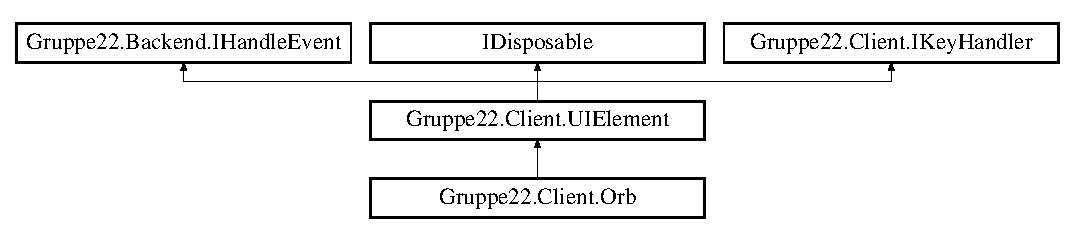
\includegraphics[height=2.692308cm]{class_gruppe22_1_1_client_1_1_orb}
\end{center}
\end{figure}
\subsection*{Öffentliche Methoden}
\begin{DoxyCompactItemize}
\item 
override void \hyperlink{class_gruppe22_1_1_client_1_1_orb_afae90f88a1d08865e47dd12413065fd4}{Update} (Game\-Time game\-Time)
\item 
override void \hyperlink{class_gruppe22_1_1_client_1_1_orb_a4254f678d8562401de35e0b285989958}{Draw} (Game\-Time gametime)
\item 
\hyperlink{class_gruppe22_1_1_client_1_1_orb_a956efd30e2eafc4e331bd663ff000a8d}{Orb} (\hyperlink{interface_gruppe22_1_1_backend_1_1_i_handle_event}{Backend.\-I\-Handle\-Event} parent, Sprite\-Batch sprite\-Batch, Content\-Manager content, Rectangle display\-Rect, int \hyperlink{class_gruppe22_1_1_client_1_1_orb_ab6d555ddf688d3bb1faae3e6a2f6dfed}{max}, int \hyperlink{class_gruppe22_1_1_client_1_1_orb_a7ed4893141f482fed4ec625869b87802}{value}, Color color)
\item 
\hyperlink{class_gruppe22_1_1_client_1_1_orb_ab8bf19b97304155601e7ad8e55bf3a96}{Orb} (\hyperlink{interface_gruppe22_1_1_backend_1_1_i_handle_event}{Backend.\-I\-Handle\-Event} parent, Sprite\-Batch sprite\-Batch, Content\-Manager content, Rectangle display\-Rect, \hyperlink{class_gruppe22_1_1_backend_1_1_actor}{Backend.\-Actor} \hyperlink{class_gruppe22_1_1_client_1_1_orb_a4e41fb8ca80e0e571c81667475c43d70}{actor}, bool is\-Magic)
\end{DoxyCompactItemize}
\subsection*{Propertys}
\begin{DoxyCompactItemize}
\item 
\hyperlink{class_gruppe22_1_1_backend_1_1_actor}{Backend.\-Actor} \hyperlink{class_gruppe22_1_1_client_1_1_orb_a4e41fb8ca80e0e571c81667475c43d70}{actor}\hspace{0.3cm}{\ttfamily  \mbox{[}get, set\mbox{]}}
\item 
int \hyperlink{class_gruppe22_1_1_client_1_1_orb_a7ed4893141f482fed4ec625869b87802}{value}\hspace{0.3cm}{\ttfamily  \mbox{[}get, set\mbox{]}}
\item 
int \hyperlink{class_gruppe22_1_1_client_1_1_orb_ab6d555ddf688d3bb1faae3e6a2f6dfed}{max}\hspace{0.3cm}{\ttfamily  \mbox{[}get, set\mbox{]}}
\end{DoxyCompactItemize}
\subsection*{Weitere Geerbte Elemente}


\subsection{Beschreibung der Konstruktoren und Destruktoren}
\hypertarget{class_gruppe22_1_1_client_1_1_orb_a956efd30e2eafc4e331bd663ff000a8d}{\index{Gruppe22\-::\-Client\-::\-Orb@{Gruppe22\-::\-Client\-::\-Orb}!Orb@{Orb}}
\index{Orb@{Orb}!Gruppe22::Client::Orb@{Gruppe22\-::\-Client\-::\-Orb}}
\subsubsection[{Orb}]{\setlength{\rightskip}{0pt plus 5cm}Gruppe22.\-Client.\-Orb.\-Orb (
\begin{DoxyParamCaption}
\item[{{\bf Backend.\-I\-Handle\-Event}}]{parent, }
\item[{Sprite\-Batch}]{sprite\-Batch, }
\item[{Content\-Manager}]{content, }
\item[{Rectangle}]{display\-Rect, }
\item[{int}]{max, }
\item[{int}]{value, }
\item[{Color}]{color}
\end{DoxyParamCaption}
)}}\label{class_gruppe22_1_1_client_1_1_orb_a956efd30e2eafc4e331bd663ff000a8d}
\hypertarget{class_gruppe22_1_1_client_1_1_orb_ab8bf19b97304155601e7ad8e55bf3a96}{\index{Gruppe22\-::\-Client\-::\-Orb@{Gruppe22\-::\-Client\-::\-Orb}!Orb@{Orb}}
\index{Orb@{Orb}!Gruppe22::Client::Orb@{Gruppe22\-::\-Client\-::\-Orb}}
\subsubsection[{Orb}]{\setlength{\rightskip}{0pt plus 5cm}Gruppe22.\-Client.\-Orb.\-Orb (
\begin{DoxyParamCaption}
\item[{{\bf Backend.\-I\-Handle\-Event}}]{parent, }
\item[{Sprite\-Batch}]{sprite\-Batch, }
\item[{Content\-Manager}]{content, }
\item[{Rectangle}]{display\-Rect, }
\item[{{\bf Backend.\-Actor}}]{actor, }
\item[{bool}]{is\-Magic}
\end{DoxyParamCaption}
)}}\label{class_gruppe22_1_1_client_1_1_orb_ab8bf19b97304155601e7ad8e55bf3a96}


\subsection{Dokumentation der Elementfunktionen}
\hypertarget{class_gruppe22_1_1_client_1_1_orb_a4254f678d8562401de35e0b285989958}{\index{Gruppe22\-::\-Client\-::\-Orb@{Gruppe22\-::\-Client\-::\-Orb}!Draw@{Draw}}
\index{Draw@{Draw}!Gruppe22::Client::Orb@{Gruppe22\-::\-Client\-::\-Orb}}
\subsubsection[{Draw}]{\setlength{\rightskip}{0pt plus 5cm}override void Gruppe22.\-Client.\-Orb.\-Draw (
\begin{DoxyParamCaption}
\item[{Game\-Time}]{game\-Time}
\end{DoxyParamCaption}
)\hspace{0.3cm}{\ttfamily [virtual]}}}\label{class_gruppe22_1_1_client_1_1_orb_a4254f678d8562401de35e0b285989958}





\begin{DoxyParams}{Parameter}
{\em game\-Time} & \\
\hline
\end{DoxyParams}


Erneute Implementation von \hyperlink{class_gruppe22_1_1_client_1_1_u_i_element_ae68afcbd1db3540052d6b399022e56e7}{Gruppe22.\-Client.\-U\-I\-Element}.

\hypertarget{class_gruppe22_1_1_client_1_1_orb_afae90f88a1d08865e47dd12413065fd4}{\index{Gruppe22\-::\-Client\-::\-Orb@{Gruppe22\-::\-Client\-::\-Orb}!Update@{Update}}
\index{Update@{Update}!Gruppe22::Client::Orb@{Gruppe22\-::\-Client\-::\-Orb}}
\subsubsection[{Update}]{\setlength{\rightskip}{0pt plus 5cm}override void Gruppe22.\-Client.\-Orb.\-Update (
\begin{DoxyParamCaption}
\item[{Game\-Time}]{game\-Time}
\end{DoxyParamCaption}
)\hspace{0.3cm}{\ttfamily [virtual]}}}\label{class_gruppe22_1_1_client_1_1_orb_afae90f88a1d08865e47dd12413065fd4}





\begin{DoxyParams}{Parameter}
{\em game\-Time} & \\
\hline
\end{DoxyParams}


Erneute Implementation von \hyperlink{class_gruppe22_1_1_client_1_1_u_i_element_a456bc763b6ed6ab441bb0ae96b6f4f8b}{Gruppe22.\-Client.\-U\-I\-Element}.



\subsection{Dokumentation der Propertys}
\hypertarget{class_gruppe22_1_1_client_1_1_orb_a4e41fb8ca80e0e571c81667475c43d70}{\index{Gruppe22\-::\-Client\-::\-Orb@{Gruppe22\-::\-Client\-::\-Orb}!actor@{actor}}
\index{actor@{actor}!Gruppe22::Client::Orb@{Gruppe22\-::\-Client\-::\-Orb}}
\subsubsection[{actor}]{\setlength{\rightskip}{0pt plus 5cm}{\bf Backend.\-Actor} Gruppe22.\-Client.\-Orb.\-actor\hspace{0.3cm}{\ttfamily [get]}, {\ttfamily [set]}}}\label{class_gruppe22_1_1_client_1_1_orb_a4e41fb8ca80e0e571c81667475c43d70}
\hypertarget{class_gruppe22_1_1_client_1_1_orb_ab6d555ddf688d3bb1faae3e6a2f6dfed}{\index{Gruppe22\-::\-Client\-::\-Orb@{Gruppe22\-::\-Client\-::\-Orb}!max@{max}}
\index{max@{max}!Gruppe22::Client::Orb@{Gruppe22\-::\-Client\-::\-Orb}}
\subsubsection[{max}]{\setlength{\rightskip}{0pt plus 5cm}int Gruppe22.\-Client.\-Orb.\-max\hspace{0.3cm}{\ttfamily [get]}, {\ttfamily [set]}}}\label{class_gruppe22_1_1_client_1_1_orb_ab6d555ddf688d3bb1faae3e6a2f6dfed}
\hypertarget{class_gruppe22_1_1_client_1_1_orb_a7ed4893141f482fed4ec625869b87802}{\index{Gruppe22\-::\-Client\-::\-Orb@{Gruppe22\-::\-Client\-::\-Orb}!value@{value}}
\index{value@{value}!Gruppe22::Client::Orb@{Gruppe22\-::\-Client\-::\-Orb}}
\subsubsection[{value}]{\setlength{\rightskip}{0pt plus 5cm}int Gruppe22.\-Client.\-Orb.\-value\hspace{0.3cm}{\ttfamily [get]}, {\ttfamily [set]}}}\label{class_gruppe22_1_1_client_1_1_orb_a7ed4893141f482fed4ec625869b87802}


Die Dokumentation für diese Klasse wurde erzeugt aufgrund der Datei\-:\begin{DoxyCompactItemize}
\item 
C\-:/\-Users/beursken/\-Documents/\-Git\-Hub/gruppe22/\-Gruppe22/\-Gruppe22/\-Client/\-U\-I/\hyperlink{_orb_8cs}{Orb.\-cs}\end{DoxyCompactItemize}

\hypertarget{class_gruppe22_1_1_backend_1_1_path}{\section{Gruppe22.\-Backend.\-Path Klassenreferenz}
\label{class_gruppe22_1_1_backend_1_1_path}\index{Gruppe22.\-Backend.\-Path@{Gruppe22.\-Backend.\-Path}}
}


A path through the maze  


Klassendiagramm für Gruppe22.\-Backend.\-Path\-:\begin{figure}[H]
\begin{center}
\leavevmode
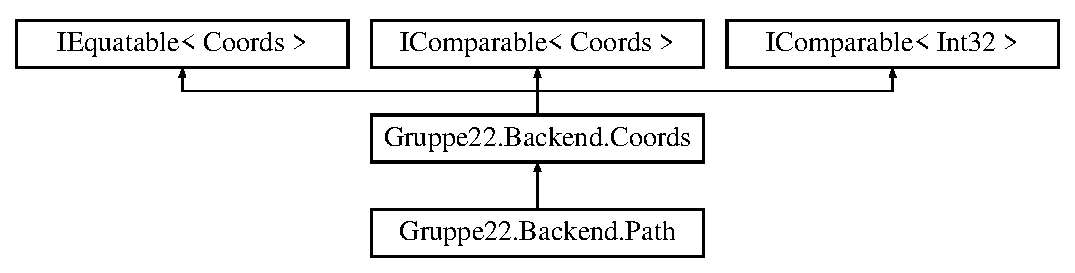
\includegraphics[height=3.000000cm]{class_gruppe22_1_1_backend_1_1_path}
\end{center}
\end{figure}
\subsection*{Öffentliche Methoden}
\begin{DoxyCompactItemize}
\item 
\hyperlink{class_gruppe22_1_1_backend_1_1_path_a5e459046dd8613e5d532ed3ec9acbf51}{Path} (int \hyperlink{class_gruppe22_1_1_backend_1_1_coords_a5d6a2857d47b7fb03ff0fa9c07a41d11}{x}=0, int \hyperlink{class_gruppe22_1_1_backend_1_1_coords_a941b0ec77fa0973cc2faf35f9a6d85dd}{y}=0, \hyperlink{namespace_gruppe22_1_1_backend_a74373668761d179b11ba50e5980a8674}{Connection} \hyperlink{class_gruppe22_1_1_backend_1_1_path_ae0b10c76528f5435bfd460892b7c1801}{dir}=Connection.\-Up)
\begin{DoxyCompactList}\small\item\em Create a new field object \end{DoxyCompactList}\end{DoxyCompactItemize}
\subsection*{Propertys}
\begin{DoxyCompactItemize}
\item 
\hyperlink{namespace_gruppe22_1_1_backend_a74373668761d179b11ba50e5980a8674}{Connection} \hyperlink{class_gruppe22_1_1_backend_1_1_path_ae0b10c76528f5435bfd460892b7c1801}{dir}\hspace{0.3cm}{\ttfamily  \mbox{[}get, set\mbox{]}}
\begin{DoxyCompactList}\small\item\em Connection to move to from current field \end{DoxyCompactList}\end{DoxyCompactItemize}
\subsection*{Weitere Geerbte Elemente}


\subsection{Ausführliche Beschreibung}
A path through the maze 



\subsection{Beschreibung der Konstruktoren und Destruktoren}
\hypertarget{class_gruppe22_1_1_backend_1_1_path_a5e459046dd8613e5d532ed3ec9acbf51}{\index{Gruppe22\-::\-Backend\-::\-Path@{Gruppe22\-::\-Backend\-::\-Path}!Path@{Path}}
\index{Path@{Path}!Gruppe22::Backend::Path@{Gruppe22\-::\-Backend\-::\-Path}}
\subsubsection[{Path}]{\setlength{\rightskip}{0pt plus 5cm}Gruppe22.\-Backend.\-Path.\-Path (
\begin{DoxyParamCaption}
\item[{int}]{x = {\ttfamily 0}, }
\item[{int}]{y = {\ttfamily 0}, }
\item[{{\bf Connection}}]{dir = {\ttfamily Connection.Up}}
\end{DoxyParamCaption}
)}}\label{class_gruppe22_1_1_backend_1_1_path_a5e459046dd8613e5d532ed3ec9acbf51}


Create a new field object 


\begin{DoxyParams}{Parameter}
{\em x} & X-\/coordinate (default 0)\\
\hline
{\em y} & Y-\/coordinate (default 0)\\
\hline
{\em dir} & Connection to move to (default\-:up)\\
\hline
\end{DoxyParams}


\subsection{Dokumentation der Propertys}
\hypertarget{class_gruppe22_1_1_backend_1_1_path_ae0b10c76528f5435bfd460892b7c1801}{\index{Gruppe22\-::\-Backend\-::\-Path@{Gruppe22\-::\-Backend\-::\-Path}!dir@{dir}}
\index{dir@{dir}!Gruppe22::Backend::Path@{Gruppe22\-::\-Backend\-::\-Path}}
\subsubsection[{dir}]{\setlength{\rightskip}{0pt plus 5cm}{\bf Connection} Gruppe22.\-Backend.\-Path.\-dir\hspace{0.3cm}{\ttfamily [get]}, {\ttfamily [set]}}}\label{class_gruppe22_1_1_backend_1_1_path_ae0b10c76528f5435bfd460892b7c1801}


Connection to move to from current field 



Die Dokumentation für diese Klasse wurde erzeugt aufgrund der Datei\-:\begin{DoxyCompactItemize}
\item 
C\-:/\-Users/beursken/\-Documents/\-Git\-Hub/gruppe22/\-Gruppe22/\-Gruppe22/\-Backend/\hyperlink{_helpers_8cs}{Helpers.\-cs}\end{DoxyCompactItemize}

\hypertarget{class_gruppe22_1_1_backend_1_1_player}{\section{Gruppe22.\-Backend.\-Player Klassenreferenz}
\label{class_gruppe22_1_1_backend_1_1_player}\index{Gruppe22.\-Backend.\-Player@{Gruppe22.\-Backend.\-Player}}
}
Klassendiagramm für Gruppe22.\-Backend.\-Player\-:\begin{figure}[H]
\begin{center}
\leavevmode
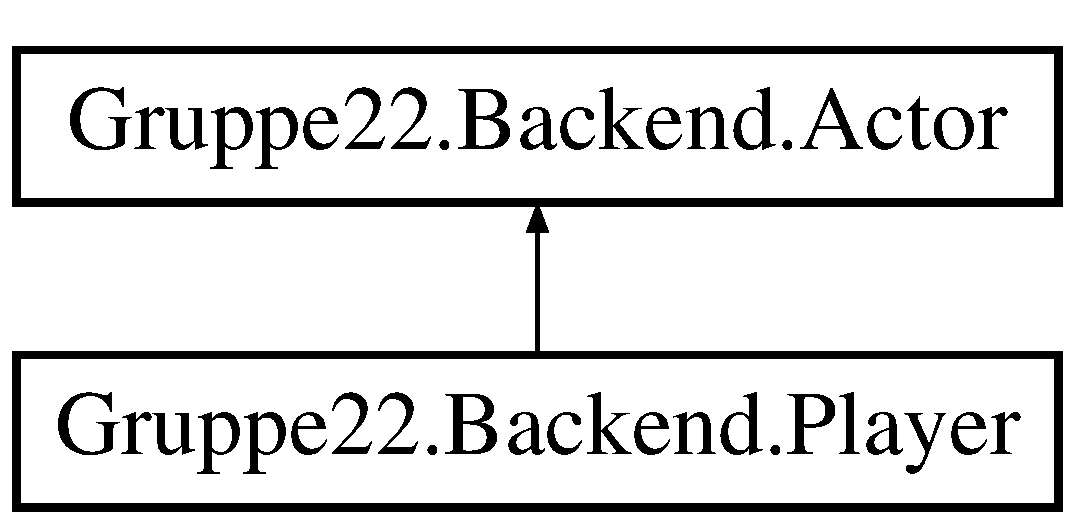
\includegraphics[height=2.000000cm]{class_gruppe22_1_1_backend_1_1_player}
\end{center}
\end{figure}
\subsection*{Öffentliche Methoden}
\begin{DoxyCompactItemize}
\item 
\hyperlink{class_gruppe22_1_1_backend_1_1_player_ae560b7beb6ae89c6cab458cdbd2cd4bf}{Player} (Content\-Manager content, int \hyperlink{class_gruppe22_1_1_backend_1_1_actor_a46f3a7d62de83a6bf3c44cd52f38af9b}{health}=100, int armour=30, int \hyperlink{class_gruppe22_1_1_backend_1_1_actor_a461e2480a59de23517c3b375dede10fb}{damage}=20, int \hyperlink{class_gruppe22_1_1_backend_1_1_actor_aac0f2f9a2f0b314f98ba19d0b38a7a97}{max\-Health}=-\/1, string \hyperlink{class_gruppe22_1_1_backend_1_1_actor_a28129eaf9d70d9bfc33a29544ba74edf}{name}=\char`\"{}\char`\"{})
\begin{DoxyCompactList}\small\item\em Constructor \end{DoxyCompactList}\end{DoxyCompactItemize}
\subsection*{Weitere Geerbte Elemente}


\subsection{Beschreibung der Konstruktoren und Destruktoren}
\hypertarget{class_gruppe22_1_1_backend_1_1_player_ae560b7beb6ae89c6cab458cdbd2cd4bf}{\index{Gruppe22\-::\-Backend\-::\-Player@{Gruppe22\-::\-Backend\-::\-Player}!Player@{Player}}
\index{Player@{Player}!Gruppe22::Backend::Player@{Gruppe22\-::\-Backend\-::\-Player}}
\subsubsection[{Player}]{\setlength{\rightskip}{0pt plus 5cm}Gruppe22.\-Backend.\-Player.\-Player (
\begin{DoxyParamCaption}
\item[{Content\-Manager}]{content, }
\item[{int}]{health = {\ttfamily 100}, }
\item[{int}]{armour = {\ttfamily 30}, }
\item[{int}]{damage = {\ttfamily 20}, }
\item[{int}]{max\-Health = {\ttfamily -\/1}, }
\item[{string}]{name = {\ttfamily \char`\"{}\char`\"{}}}
\end{DoxyParamCaption}
)}}\label{class_gruppe22_1_1_backend_1_1_player_ae560b7beb6ae89c6cab458cdbd2cd4bf}


Constructor 



Die Dokumentation für diese Klasse wurde erzeugt aufgrund der Datei\-:\begin{DoxyCompactItemize}
\item 
C\-:/\-Users/beursken/\-Documents/\-Git\-Hub/gruppe22/\-Gruppe22/\-Gruppe22/\-Backend/\-Actors/\hyperlink{_player_8cs}{Player.\-cs}\end{DoxyCompactItemize}

\hypertarget{class_gruppe22_1_1_client_1_1_progress_bar}{\section{Gruppe22.\-Client.\-Progress\-Bar Klassenreferenz}
\label{class_gruppe22_1_1_client_1_1_progress_bar}\index{Gruppe22.\-Client.\-Progress\-Bar@{Gruppe22.\-Client.\-Progress\-Bar}}
}


A progress bar  


Klassendiagramm für Gruppe22.\-Client.\-Progress\-Bar\-:\begin{figure}[H]
\begin{center}
\leavevmode
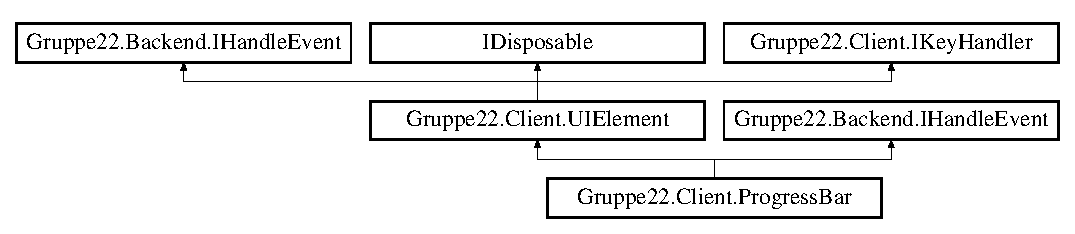
\includegraphics[height=2.692308cm]{class_gruppe22_1_1_client_1_1_progress_bar}
\end{center}
\end{figure}
\subsection*{Öffentliche Methoden}
\begin{DoxyCompactItemize}
\item 
override bool \hyperlink{class_gruppe22_1_1_client_1_1_progress_bar_a71b7f2b9c567a74a3a27ed2efec9b346}{Is\-Hit} (int x, int y)
\begin{DoxyCompactList}\small\item\em Check whether a pixel is part of the window \end{DoxyCompactList}\item 
override void \hyperlink{class_gruppe22_1_1_client_1_1_progress_bar_ad0729c9280a779e37797f5342d374993}{Draw} (Game\-Time game\-Time)
\begin{DoxyCompactList}\small\item\em Display the progressbar using appropriate position,style and color \end{DoxyCompactList}\item 
override void \hyperlink{class_gruppe22_1_1_client_1_1_progress_bar_ac1f470e3a5fa29d2b408e3617e0a5f19}{Update} (Game\-Time game\-Time)
\begin{DoxyCompactList}\small\item\em Move progress bar (if animated) \end{DoxyCompactList}\item 
\hyperlink{class_gruppe22_1_1_client_1_1_progress_bar_a9f09493570ef928d80d1d62d20dcccf4}{Progress\-Bar} (\hyperlink{interface_gruppe22_1_1_backend_1_1_i_handle_event}{Backend.\-I\-Handle\-Event} parent, Sprite\-Batch sprite\-Batch, Content\-Manager content, Rectangle display\-Rect, \hyperlink{namespace_gruppe22_1_1_client_a4f652636831acdc7988060a3c213d941}{Progress\-Style} style=Progress\-Style.\-Default, int \hyperlink{class_gruppe22_1_1_client_1_1_progress_bar_ae3302bc227446998679b7e4a0f67f9bb}{total}=100, int start=0)
\begin{DoxyCompactList}\small\item\em Create a new progress bar \end{DoxyCompactList}\end{DoxyCompactItemize}
\subsection*{Propertys}
\begin{DoxyCompactItemize}
\item 
int \hyperlink{class_gruppe22_1_1_client_1_1_progress_bar_a01b5256bfaae8452ff2cbc7db92adc8a}{value}\hspace{0.3cm}{\ttfamily  \mbox{[}get, set\mbox{]}}
\begin{DoxyCompactList}\small\item\em Current value of the progress bar (minimum 0, maximum set by total) \end{DoxyCompactList}\item 
int \hyperlink{class_gruppe22_1_1_client_1_1_progress_bar_ae3302bc227446998679b7e4a0f67f9bb}{total}\hspace{0.3cm}{\ttfamily  \mbox{[}get, set\mbox{]}}
\begin{DoxyCompactList}\small\item\em Total amount available on the progress bar (resets value) \end{DoxyCompactList}\item 
override bool \hyperlink{class_gruppe22_1_1_client_1_1_progress_bar_ab1cf4a6b7055b48199edac21328ae1ed}{ignore\-Pause}\hspace{0.3cm}{\ttfamily  \mbox{[}get\mbox{]}}
\begin{DoxyCompactList}\small\item\em Progress bars animate and display even if program is paused \end{DoxyCompactList}\item 
Color \hyperlink{class_gruppe22_1_1_client_1_1_progress_bar_a0af6ea002815cac6dbc030d5fb1de81d}{color}\hspace{0.3cm}{\ttfamily  \mbox{[}get, set\mbox{]}}
\end{DoxyCompactItemize}
\subsection*{Weitere Geerbte Elemente}


\subsection{Ausführliche Beschreibung}
A progress bar 



\subsection{Beschreibung der Konstruktoren und Destruktoren}
\hypertarget{class_gruppe22_1_1_client_1_1_progress_bar_a9f09493570ef928d80d1d62d20dcccf4}{\index{Gruppe22\-::\-Client\-::\-Progress\-Bar@{Gruppe22\-::\-Client\-::\-Progress\-Bar}!Progress\-Bar@{Progress\-Bar}}
\index{Progress\-Bar@{Progress\-Bar}!Gruppe22::Client::ProgressBar@{Gruppe22\-::\-Client\-::\-Progress\-Bar}}
\subsubsection[{Progress\-Bar}]{\setlength{\rightskip}{0pt plus 5cm}Gruppe22.\-Client.\-Progress\-Bar.\-Progress\-Bar (
\begin{DoxyParamCaption}
\item[{{\bf Backend.\-I\-Handle\-Event}}]{parent, }
\item[{Sprite\-Batch}]{sprite\-Batch, }
\item[{Content\-Manager}]{content, }
\item[{Rectangle}]{display\-Rect, }
\item[{{\bf Progress\-Style}}]{style = {\ttfamily ProgressStyle.Default}, }
\item[{int}]{total = {\ttfamily 100}, }
\item[{int}]{start = {\ttfamily 0}}
\end{DoxyParamCaption}
)}}\label{class_gruppe22_1_1_client_1_1_progress_bar_a9f09493570ef928d80d1d62d20dcccf4}


Create a new progress bar 


\begin{DoxyParams}{Parameter}
{\em parent} & A parent object to pass events to\\
\hline
{\em sprite\-Batch} & A spritebatch used for drawing\\
\hline
{\em content} & A Contentmanager used for loading resources\\
\hline
{\em display\-Rect} & The area of the progress bar\\
\hline
{\em style} & The design of the progress bar\\
\hline
{\em total} & A maximum amount to be displayed on the progress bar\\
\hline
{\em start} & The start value\\
\hline
{\em color} & The color of the progress bar\\
\hline
\end{DoxyParams}


\subsection{Dokumentation der Elementfunktionen}
\hypertarget{class_gruppe22_1_1_client_1_1_progress_bar_ad0729c9280a779e37797f5342d374993}{\index{Gruppe22\-::\-Client\-::\-Progress\-Bar@{Gruppe22\-::\-Client\-::\-Progress\-Bar}!Draw@{Draw}}
\index{Draw@{Draw}!Gruppe22::Client::ProgressBar@{Gruppe22\-::\-Client\-::\-Progress\-Bar}}
\subsubsection[{Draw}]{\setlength{\rightskip}{0pt plus 5cm}override void Gruppe22.\-Client.\-Progress\-Bar.\-Draw (
\begin{DoxyParamCaption}
\item[{Game\-Time}]{game\-Time}
\end{DoxyParamCaption}
)\hspace{0.3cm}{\ttfamily [virtual]}}}\label{class_gruppe22_1_1_client_1_1_progress_bar_ad0729c9280a779e37797f5342d374993}


Display the progressbar using appropriate position,style and color 


\begin{DoxyParams}{Parameter}
{\em game\-Time} & \\
\hline
\end{DoxyParams}


Erneute Implementation von \hyperlink{class_gruppe22_1_1_client_1_1_u_i_element_ae68afcbd1db3540052d6b399022e56e7}{Gruppe22.\-Client.\-U\-I\-Element}.

\hypertarget{class_gruppe22_1_1_client_1_1_progress_bar_a71b7f2b9c567a74a3a27ed2efec9b346}{\index{Gruppe22\-::\-Client\-::\-Progress\-Bar@{Gruppe22\-::\-Client\-::\-Progress\-Bar}!Is\-Hit@{Is\-Hit}}
\index{Is\-Hit@{Is\-Hit}!Gruppe22::Client::ProgressBar@{Gruppe22\-::\-Client\-::\-Progress\-Bar}}
\subsubsection[{Is\-Hit}]{\setlength{\rightskip}{0pt plus 5cm}override bool Gruppe22.\-Client.\-Progress\-Bar.\-Is\-Hit (
\begin{DoxyParamCaption}
\item[{int}]{x, }
\item[{int}]{y}
\end{DoxyParamCaption}
)\hspace{0.3cm}{\ttfamily [virtual]}}}\label{class_gruppe22_1_1_client_1_1_progress_bar_a71b7f2b9c567a74a3a27ed2efec9b346}


Check whether a pixel is part of the window 


\begin{DoxyParams}{Parameter}
{\em x} & Horizontal coordinate\\
\hline
{\em y} & Vertical coordinate\\
\hline
\end{DoxyParams}
\begin{DoxyReturn}{Rückgabe}
true if pixel is part of the window
\end{DoxyReturn}


Erneute Implementation von \hyperlink{class_gruppe22_1_1_client_1_1_u_i_element_a3be972299c1d8b6f7518b833f5c98992}{Gruppe22.\-Client.\-U\-I\-Element}.

\hypertarget{class_gruppe22_1_1_client_1_1_progress_bar_ac1f470e3a5fa29d2b408e3617e0a5f19}{\index{Gruppe22\-::\-Client\-::\-Progress\-Bar@{Gruppe22\-::\-Client\-::\-Progress\-Bar}!Update@{Update}}
\index{Update@{Update}!Gruppe22::Client::ProgressBar@{Gruppe22\-::\-Client\-::\-Progress\-Bar}}
\subsubsection[{Update}]{\setlength{\rightskip}{0pt plus 5cm}override void Gruppe22.\-Client.\-Progress\-Bar.\-Update (
\begin{DoxyParamCaption}
\item[{Game\-Time}]{game\-Time}
\end{DoxyParamCaption}
)\hspace{0.3cm}{\ttfamily [virtual]}}}\label{class_gruppe22_1_1_client_1_1_progress_bar_ac1f470e3a5fa29d2b408e3617e0a5f19}


Move progress bar (if animated) 


\begin{DoxyParams}{Parameter}
{\em game\-Time} & \\
\hline
\end{DoxyParams}


Erneute Implementation von \hyperlink{class_gruppe22_1_1_client_1_1_u_i_element_a456bc763b6ed6ab441bb0ae96b6f4f8b}{Gruppe22.\-Client.\-U\-I\-Element}.



\subsection{Dokumentation der Propertys}
\hypertarget{class_gruppe22_1_1_client_1_1_progress_bar_a0af6ea002815cac6dbc030d5fb1de81d}{\index{Gruppe22\-::\-Client\-::\-Progress\-Bar@{Gruppe22\-::\-Client\-::\-Progress\-Bar}!color@{color}}
\index{color@{color}!Gruppe22::Client::ProgressBar@{Gruppe22\-::\-Client\-::\-Progress\-Bar}}
\subsubsection[{color}]{\setlength{\rightskip}{0pt plus 5cm}Color Gruppe22.\-Client.\-Progress\-Bar.\-color\hspace{0.3cm}{\ttfamily [get]}, {\ttfamily [set]}}}\label{class_gruppe22_1_1_client_1_1_progress_bar_a0af6ea002815cac6dbc030d5fb1de81d}
\hypertarget{class_gruppe22_1_1_client_1_1_progress_bar_ab1cf4a6b7055b48199edac21328ae1ed}{\index{Gruppe22\-::\-Client\-::\-Progress\-Bar@{Gruppe22\-::\-Client\-::\-Progress\-Bar}!ignore\-Pause@{ignore\-Pause}}
\index{ignore\-Pause@{ignore\-Pause}!Gruppe22::Client::ProgressBar@{Gruppe22\-::\-Client\-::\-Progress\-Bar}}
\subsubsection[{ignore\-Pause}]{\setlength{\rightskip}{0pt plus 5cm}override bool Gruppe22.\-Client.\-Progress\-Bar.\-ignore\-Pause\hspace{0.3cm}{\ttfamily [get]}}}\label{class_gruppe22_1_1_client_1_1_progress_bar_ab1cf4a6b7055b48199edac21328ae1ed}


Progress bars animate and display even if program is paused 

\hypertarget{class_gruppe22_1_1_client_1_1_progress_bar_ae3302bc227446998679b7e4a0f67f9bb}{\index{Gruppe22\-::\-Client\-::\-Progress\-Bar@{Gruppe22\-::\-Client\-::\-Progress\-Bar}!total@{total}}
\index{total@{total}!Gruppe22::Client::ProgressBar@{Gruppe22\-::\-Client\-::\-Progress\-Bar}}
\subsubsection[{total}]{\setlength{\rightskip}{0pt plus 5cm}int Gruppe22.\-Client.\-Progress\-Bar.\-total\hspace{0.3cm}{\ttfamily [get]}, {\ttfamily [set]}}}\label{class_gruppe22_1_1_client_1_1_progress_bar_ae3302bc227446998679b7e4a0f67f9bb}


Total amount available on the progress bar (resets value) 

\hypertarget{class_gruppe22_1_1_client_1_1_progress_bar_a01b5256bfaae8452ff2cbc7db92adc8a}{\index{Gruppe22\-::\-Client\-::\-Progress\-Bar@{Gruppe22\-::\-Client\-::\-Progress\-Bar}!value@{value}}
\index{value@{value}!Gruppe22::Client::ProgressBar@{Gruppe22\-::\-Client\-::\-Progress\-Bar}}
\subsubsection[{value}]{\setlength{\rightskip}{0pt plus 5cm}int Gruppe22.\-Client.\-Progress\-Bar.\-value\hspace{0.3cm}{\ttfamily [get]}, {\ttfamily [set]}}}\label{class_gruppe22_1_1_client_1_1_progress_bar_a01b5256bfaae8452ff2cbc7db92adc8a}


Current value of the progress bar (minimum 0, maximum set by total) 



Die Dokumentation für diese Klasse wurde erzeugt aufgrund der Datei\-:\begin{DoxyCompactItemize}
\item 
C\-:/\-Users/beursken/\-Documents/\-Git\-Hub/gruppe22/\-Gruppe22/\-Gruppe22/\-Client/\-U\-I/\hyperlink{_progressbar_8cs}{Progressbar.\-cs}\end{DoxyCompactItemize}

\hypertarget{class_gruppe22_1_1_client_1_1_projectile}{\section{Gruppe22.\-Client.\-Projectile Klassenreferenz}
\label{class_gruppe22_1_1_client_1_1_projectile}\index{Gruppe22.\-Client.\-Projectile@{Gruppe22.\-Client.\-Projectile}}
}
\subsection*{Öffentliche Methoden}
\begin{DoxyCompactItemize}
\item 
void \hyperlink{class_gruppe22_1_1_client_1_1_projectile_a754c50d48c5c1667691fa494d20a0583}{move\-To} (\hyperlink{class_gruppe22_1_1_backend_1_1_coords}{Backend.\-Coords} coord)
\item 
void \hyperlink{class_gruppe22_1_1_client_1_1_projectile_a9870a8bba637e177cfd60a8ed363f542}{Draw} ()
\item 
void \hyperlink{class_gruppe22_1_1_client_1_1_projectile_a37ff55bb3fd3fb071c1a4a7a1262e25d}{Update} (Game\-Time gametime)
\item 
void \hyperlink{class_gruppe22_1_1_client_1_1_projectile_addca7438b89e11199d66ffbdb4d201b6}{Draw} (Sprite\-Batch \-\_\-sprite\-Batch, \hyperlink{class_gruppe22_1_1_client_1_1_tile_object}{Tile\-Object} animation)
\item 
\hyperlink{class_gruppe22_1_1_client_1_1_projectile_a462e1a1ed97ee8a68cc59f931ac721f0}{Projectile} (uint \hyperlink{class_gruppe22_1_1_client_1_1_projectile_ab29686eea9206ed8e87f1d65ec1c9993}{id}, \hyperlink{interface_gruppe22_1_1_backend_1_1_i_handle_event}{Backend.\-I\-Handle\-Event} parent, \hyperlink{class_gruppe22_1_1_backend_1_1_coords}{Backend.\-Coords} current, \hyperlink{namespace_gruppe22_1_1_backend_a2d53d5d14b8ea0951ba6971e5da1ebf5}{Backend.\-Direction} dir, \hyperlink{class_gruppe22_1_1_projectile_tile}{Projectile\-Tile} \hyperlink{class_gruppe22_1_1_client_1_1_projectile_a4f6302a03a806ca00bce450bb715d405}{tile})
\end{DoxyCompactItemize}
\subsection*{Öffentliche Attribute}
\begin{DoxyCompactItemize}
\item 
uint \hyperlink{class_gruppe22_1_1_client_1_1_projectile_a5ca3b8028011f80a8c631abe434cc1c9}{\-\_\-elapsed} = 0
\item 
bool \hyperlink{class_gruppe22_1_1_client_1_1_projectile_a971577dac5c8af89967628cfc571223e}{\-\_\-nomove} = false
\item 
\hyperlink{interface_gruppe22_1_1_backend_1_1_i_handle_event}{Backend.\-I\-Handle\-Event} \hyperlink{class_gruppe22_1_1_client_1_1_projectile_a7fd18cd246a687bde87f648ff8bfabca}{\-\_\-parent}
\end{DoxyCompactItemize}
\subsection*{Propertys}
\begin{DoxyCompactItemize}
\item 
uint \hyperlink{class_gruppe22_1_1_client_1_1_projectile_ab29686eea9206ed8e87f1d65ec1c9993}{id}\hspace{0.3cm}{\ttfamily  \mbox{[}get, set\mbox{]}}
\item 
int \hyperlink{class_gruppe22_1_1_client_1_1_projectile_acb7573c8fa44d4181052c43357203115}{direction}\hspace{0.3cm}{\ttfamily  \mbox{[}get\mbox{]}}
\item 
\hyperlink{class_gruppe22_1_1_projectile_tile}{Projectile\-Tile} \hyperlink{class_gruppe22_1_1_client_1_1_projectile_a4f6302a03a806ca00bce450bb715d405}{tile}\hspace{0.3cm}{\ttfamily  \mbox{[}get, set\mbox{]}}
\end{DoxyCompactItemize}


\subsection{Beschreibung der Konstruktoren und Destruktoren}
\hypertarget{class_gruppe22_1_1_client_1_1_projectile_a462e1a1ed97ee8a68cc59f931ac721f0}{\index{Gruppe22\-::\-Client\-::\-Projectile@{Gruppe22\-::\-Client\-::\-Projectile}!Projectile@{Projectile}}
\index{Projectile@{Projectile}!Gruppe22::Client::Projectile@{Gruppe22\-::\-Client\-::\-Projectile}}
\subsubsection[{Projectile}]{\setlength{\rightskip}{0pt plus 5cm}Gruppe22.\-Client.\-Projectile.\-Projectile (
\begin{DoxyParamCaption}
\item[{uint}]{id, }
\item[{{\bf Backend.\-I\-Handle\-Event}}]{parent, }
\item[{{\bf Backend.\-Coords}}]{current, }
\item[{{\bf Backend.\-Direction}}]{dir, }
\item[{{\bf Projectile\-Tile}}]{tile}
\end{DoxyParamCaption}
)}}\label{class_gruppe22_1_1_client_1_1_projectile_a462e1a1ed97ee8a68cc59f931ac721f0}


\subsection{Dokumentation der Elementfunktionen}
\hypertarget{class_gruppe22_1_1_client_1_1_projectile_a9870a8bba637e177cfd60a8ed363f542}{\index{Gruppe22\-::\-Client\-::\-Projectile@{Gruppe22\-::\-Client\-::\-Projectile}!Draw@{Draw}}
\index{Draw@{Draw}!Gruppe22::Client::Projectile@{Gruppe22\-::\-Client\-::\-Projectile}}
\subsubsection[{Draw}]{\setlength{\rightskip}{0pt plus 5cm}void Gruppe22.\-Client.\-Projectile.\-Draw (
\begin{DoxyParamCaption}
{}
\end{DoxyParamCaption}
)}}\label{class_gruppe22_1_1_client_1_1_projectile_a9870a8bba637e177cfd60a8ed363f542}
\hypertarget{class_gruppe22_1_1_client_1_1_projectile_addca7438b89e11199d66ffbdb4d201b6}{\index{Gruppe22\-::\-Client\-::\-Projectile@{Gruppe22\-::\-Client\-::\-Projectile}!Draw@{Draw}}
\index{Draw@{Draw}!Gruppe22::Client::Projectile@{Gruppe22\-::\-Client\-::\-Projectile}}
\subsubsection[{Draw}]{\setlength{\rightskip}{0pt plus 5cm}void Gruppe22.\-Client.\-Projectile.\-Draw (
\begin{DoxyParamCaption}
\item[{Sprite\-Batch}]{\-\_\-sprite\-Batch, }
\item[{{\bf Tile\-Object}}]{animation}
\end{DoxyParamCaption}
)}}\label{class_gruppe22_1_1_client_1_1_projectile_addca7438b89e11199d66ffbdb4d201b6}
\hypertarget{class_gruppe22_1_1_client_1_1_projectile_a754c50d48c5c1667691fa494d20a0583}{\index{Gruppe22\-::\-Client\-::\-Projectile@{Gruppe22\-::\-Client\-::\-Projectile}!move\-To@{move\-To}}
\index{move\-To@{move\-To}!Gruppe22::Client::Projectile@{Gruppe22\-::\-Client\-::\-Projectile}}
\subsubsection[{move\-To}]{\setlength{\rightskip}{0pt plus 5cm}void Gruppe22.\-Client.\-Projectile.\-move\-To (
\begin{DoxyParamCaption}
\item[{{\bf Backend.\-Coords}}]{coord}
\end{DoxyParamCaption}
)}}\label{class_gruppe22_1_1_client_1_1_projectile_a754c50d48c5c1667691fa494d20a0583}
\hypertarget{class_gruppe22_1_1_client_1_1_projectile_a37ff55bb3fd3fb071c1a4a7a1262e25d}{\index{Gruppe22\-::\-Client\-::\-Projectile@{Gruppe22\-::\-Client\-::\-Projectile}!Update@{Update}}
\index{Update@{Update}!Gruppe22::Client::Projectile@{Gruppe22\-::\-Client\-::\-Projectile}}
\subsubsection[{Update}]{\setlength{\rightskip}{0pt plus 5cm}void Gruppe22.\-Client.\-Projectile.\-Update (
\begin{DoxyParamCaption}
\item[{Game\-Time}]{gametime}
\end{DoxyParamCaption}
)}}\label{class_gruppe22_1_1_client_1_1_projectile_a37ff55bb3fd3fb071c1a4a7a1262e25d}


\subsection{Dokumentation der Datenelemente}
\hypertarget{class_gruppe22_1_1_client_1_1_projectile_a5ca3b8028011f80a8c631abe434cc1c9}{\index{Gruppe22\-::\-Client\-::\-Projectile@{Gruppe22\-::\-Client\-::\-Projectile}!\-\_\-elapsed@{\-\_\-elapsed}}
\index{\-\_\-elapsed@{\-\_\-elapsed}!Gruppe22::Client::Projectile@{Gruppe22\-::\-Client\-::\-Projectile}}
\subsubsection[{\-\_\-elapsed}]{\setlength{\rightskip}{0pt plus 5cm}uint Gruppe22.\-Client.\-Projectile.\-\_\-elapsed = 0}}\label{class_gruppe22_1_1_client_1_1_projectile_a5ca3b8028011f80a8c631abe434cc1c9}
\hypertarget{class_gruppe22_1_1_client_1_1_projectile_a971577dac5c8af89967628cfc571223e}{\index{Gruppe22\-::\-Client\-::\-Projectile@{Gruppe22\-::\-Client\-::\-Projectile}!\-\_\-nomove@{\-\_\-nomove}}
\index{\-\_\-nomove@{\-\_\-nomove}!Gruppe22::Client::Projectile@{Gruppe22\-::\-Client\-::\-Projectile}}
\subsubsection[{\-\_\-nomove}]{\setlength{\rightskip}{0pt plus 5cm}bool Gruppe22.\-Client.\-Projectile.\-\_\-nomove = false}}\label{class_gruppe22_1_1_client_1_1_projectile_a971577dac5c8af89967628cfc571223e}
\hypertarget{class_gruppe22_1_1_client_1_1_projectile_a7fd18cd246a687bde87f648ff8bfabca}{\index{Gruppe22\-::\-Client\-::\-Projectile@{Gruppe22\-::\-Client\-::\-Projectile}!\-\_\-parent@{\-\_\-parent}}
\index{\-\_\-parent@{\-\_\-parent}!Gruppe22::Client::Projectile@{Gruppe22\-::\-Client\-::\-Projectile}}
\subsubsection[{\-\_\-parent}]{\setlength{\rightskip}{0pt plus 5cm}{\bf Backend.\-I\-Handle\-Event} Gruppe22.\-Client.\-Projectile.\-\_\-parent}}\label{class_gruppe22_1_1_client_1_1_projectile_a7fd18cd246a687bde87f648ff8bfabca}


\subsection{Dokumentation der Propertys}
\hypertarget{class_gruppe22_1_1_client_1_1_projectile_acb7573c8fa44d4181052c43357203115}{\index{Gruppe22\-::\-Client\-::\-Projectile@{Gruppe22\-::\-Client\-::\-Projectile}!direction@{direction}}
\index{direction@{direction}!Gruppe22::Client::Projectile@{Gruppe22\-::\-Client\-::\-Projectile}}
\subsubsection[{direction}]{\setlength{\rightskip}{0pt plus 5cm}int Gruppe22.\-Client.\-Projectile.\-direction\hspace{0.3cm}{\ttfamily [get]}}}\label{class_gruppe22_1_1_client_1_1_projectile_acb7573c8fa44d4181052c43357203115}
\hypertarget{class_gruppe22_1_1_client_1_1_projectile_ab29686eea9206ed8e87f1d65ec1c9993}{\index{Gruppe22\-::\-Client\-::\-Projectile@{Gruppe22\-::\-Client\-::\-Projectile}!id@{id}}
\index{id@{id}!Gruppe22::Client::Projectile@{Gruppe22\-::\-Client\-::\-Projectile}}
\subsubsection[{id}]{\setlength{\rightskip}{0pt plus 5cm}uint Gruppe22.\-Client.\-Projectile.\-id\hspace{0.3cm}{\ttfamily [get]}, {\ttfamily [set]}}}\label{class_gruppe22_1_1_client_1_1_projectile_ab29686eea9206ed8e87f1d65ec1c9993}
\hypertarget{class_gruppe22_1_1_client_1_1_projectile_a4f6302a03a806ca00bce450bb715d405}{\index{Gruppe22\-::\-Client\-::\-Projectile@{Gruppe22\-::\-Client\-::\-Projectile}!tile@{tile}}
\index{tile@{tile}!Gruppe22::Client::Projectile@{Gruppe22\-::\-Client\-::\-Projectile}}
\subsubsection[{tile}]{\setlength{\rightskip}{0pt plus 5cm}{\bf Projectile\-Tile} Gruppe22.\-Client.\-Projectile.\-tile\hspace{0.3cm}{\ttfamily [get]}, {\ttfamily [set]}}}\label{class_gruppe22_1_1_client_1_1_projectile_a4f6302a03a806ca00bce450bb715d405}


Die Dokumentation für diese Klasse wurde erzeugt aufgrund der Datei\-:\begin{DoxyCompactItemize}
\item 
C\-:/\-Users/beursken/\-Documents/\-Git\-Hub/gruppe22/\-Gruppe22/\-Gruppe22/\-Client/\-Map/\hyperlink{_mainmap_8cs}{Mainmap.\-cs}\end{DoxyCompactItemize}

\hypertarget{class_gruppe22_1_1_projectile_tile}{\section{Gruppe22.\-Projectile\-Tile Klassenreferenz}
\label{class_gruppe22_1_1_projectile_tile}\index{Gruppe22.\-Projectile\-Tile@{Gruppe22.\-Projectile\-Tile}}
}
Klassendiagramm für Gruppe22.\-Projectile\-Tile\-:\begin{figure}[H]
\begin{center}
\leavevmode
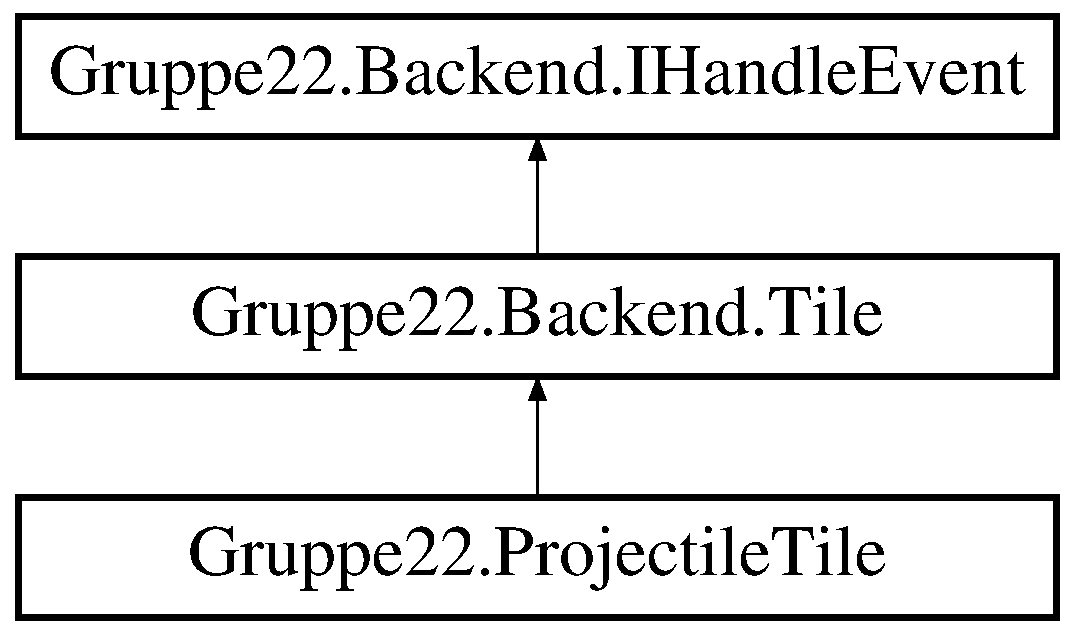
\includegraphics[height=3.000000cm]{class_gruppe22_1_1_projectile_tile}
\end{center}
\end{figure}
\subsection*{Öffentliche Methoden}
\begin{DoxyCompactItemize}
\item 
\hyperlink{class_gruppe22_1_1_projectile_tile_ac5602e794c82c68d7bfa47af9634ee09}{Projectile\-Tile} (\hyperlink{class_gruppe22_1_1_backend_1_1_floor_tile}{Backend.\-Floor\-Tile} \hyperlink{class_gruppe22_1_1_backend_1_1_tile_abc12933c70eb3a2ebbb2fde9f45c2632}{parent}, \hyperlink{namespace_gruppe22_1_1_backend_a2d53d5d14b8ea0951ba6971e5da1ebf5}{Backend.\-Direction} dir, uint \hyperlink{class_gruppe22_1_1_projectile_tile_ab9b7a588cb5132cd66a09bef09616bb2}{id}=0)
\item 
void \hyperlink{class_gruppe22_1_1_projectile_tile_a342aab74a5f512ba72d754615134bb7a}{Next\-Tile} (bool do\-Move=false)
\item 
override void \hyperlink{class_gruppe22_1_1_projectile_tile_ac04e7d0bab385f083a1d4dca56083f3d}{Save} (Xml\-Writer xmlw)
\begin{DoxyCompactList}\small\item\em Abstract method to save a tile in a X\-M\-L file \end{DoxyCompactList}\end{DoxyCompactItemize}
\subsection*{Propertys}
\begin{DoxyCompactItemize}
\item 
uint \hyperlink{class_gruppe22_1_1_projectile_tile_ab9b7a588cb5132cd66a09bef09616bb2}{id}\hspace{0.3cm}{\ttfamily  \mbox{[}get, set\mbox{]}}
\end{DoxyCompactItemize}
\subsection*{Weitere Geerbte Elemente}


\subsection{Beschreibung der Konstruktoren und Destruktoren}
\hypertarget{class_gruppe22_1_1_projectile_tile_ac5602e794c82c68d7bfa47af9634ee09}{\index{Gruppe22\-::\-Projectile\-Tile@{Gruppe22\-::\-Projectile\-Tile}!Projectile\-Tile@{Projectile\-Tile}}
\index{Projectile\-Tile@{Projectile\-Tile}!Gruppe22::ProjectileTile@{Gruppe22\-::\-Projectile\-Tile}}
\subsubsection[{Projectile\-Tile}]{\setlength{\rightskip}{0pt plus 5cm}Gruppe22.\-Projectile\-Tile.\-Projectile\-Tile (
\begin{DoxyParamCaption}
\item[{{\bf Backend.\-Floor\-Tile}}]{parent, }
\item[{{\bf Backend.\-Direction}}]{dir, }
\item[{uint}]{id = {\ttfamily 0}}
\end{DoxyParamCaption}
)}}\label{class_gruppe22_1_1_projectile_tile_ac5602e794c82c68d7bfa47af9634ee09}


\subsection{Dokumentation der Elementfunktionen}
\hypertarget{class_gruppe22_1_1_projectile_tile_a342aab74a5f512ba72d754615134bb7a}{\index{Gruppe22\-::\-Projectile\-Tile@{Gruppe22\-::\-Projectile\-Tile}!Next\-Tile@{Next\-Tile}}
\index{Next\-Tile@{Next\-Tile}!Gruppe22::ProjectileTile@{Gruppe22\-::\-Projectile\-Tile}}
\subsubsection[{Next\-Tile}]{\setlength{\rightskip}{0pt plus 5cm}void Gruppe22.\-Projectile\-Tile.\-Next\-Tile (
\begin{DoxyParamCaption}
\item[{bool}]{do\-Move = {\ttfamily false}}
\end{DoxyParamCaption}
)}}\label{class_gruppe22_1_1_projectile_tile_a342aab74a5f512ba72d754615134bb7a}
\hypertarget{class_gruppe22_1_1_projectile_tile_ac04e7d0bab385f083a1d4dca56083f3d}{\index{Gruppe22\-::\-Projectile\-Tile@{Gruppe22\-::\-Projectile\-Tile}!Save@{Save}}
\index{Save@{Save}!Gruppe22::ProjectileTile@{Gruppe22\-::\-Projectile\-Tile}}
\subsubsection[{Save}]{\setlength{\rightskip}{0pt plus 5cm}override void Gruppe22.\-Projectile\-Tile.\-Save (
\begin{DoxyParamCaption}
\item[{Xml\-Writer}]{xmlw}
\end{DoxyParamCaption}
)\hspace{0.3cm}{\ttfamily [virtual]}}}\label{class_gruppe22_1_1_projectile_tile_ac04e7d0bab385f083a1d4dca56083f3d}


Abstract method to save a tile in a X\-M\-L file 


\begin{DoxyParams}{Parameter}
{\em xmlw} & the Xml\-Writer used for saving the file\\
\hline
\end{DoxyParams}


Erneute Implementation von \hyperlink{class_gruppe22_1_1_backend_1_1_tile_a109ab3e77ffca9d44c95a711af3491dc}{Gruppe22.\-Backend.\-Tile}.



\subsection{Dokumentation der Propertys}
\hypertarget{class_gruppe22_1_1_projectile_tile_ab9b7a588cb5132cd66a09bef09616bb2}{\index{Gruppe22\-::\-Projectile\-Tile@{Gruppe22\-::\-Projectile\-Tile}!id@{id}}
\index{id@{id}!Gruppe22::ProjectileTile@{Gruppe22\-::\-Projectile\-Tile}}
\subsubsection[{id}]{\setlength{\rightskip}{0pt plus 5cm}uint Gruppe22.\-Projectile\-Tile.\-id\hspace{0.3cm}{\ttfamily [get]}, {\ttfamily [set]}}}\label{class_gruppe22_1_1_projectile_tile_ab9b7a588cb5132cd66a09bef09616bb2}


Die Dokumentation für diese Klasse wurde erzeugt aufgrund der Datei\-:\begin{DoxyCompactItemize}
\item 
C\-:/\-Users/beursken/\-Documents/\-Git\-Hub/gruppe22/\-Gruppe22/\-Gruppe22/\-Backend/\-Map/\hyperlink{_projectile_tile_8cs}{Projectile\-Tile.\-cs}\end{DoxyCompactItemize}

\hypertarget{class_gruppe22_1_1_backend_1_1_reserved_tile}{\section{Gruppe22.\-Backend.\-Reserved\-Tile Klassenreferenz}
\label{class_gruppe22_1_1_backend_1_1_reserved_tile}\index{Gruppe22.\-Backend.\-Reserved\-Tile@{Gruppe22.\-Backend.\-Reserved\-Tile}}
}
Klassendiagramm für Gruppe22.\-Backend.\-Reserved\-Tile\-:\begin{figure}[H]
\begin{center}
\leavevmode
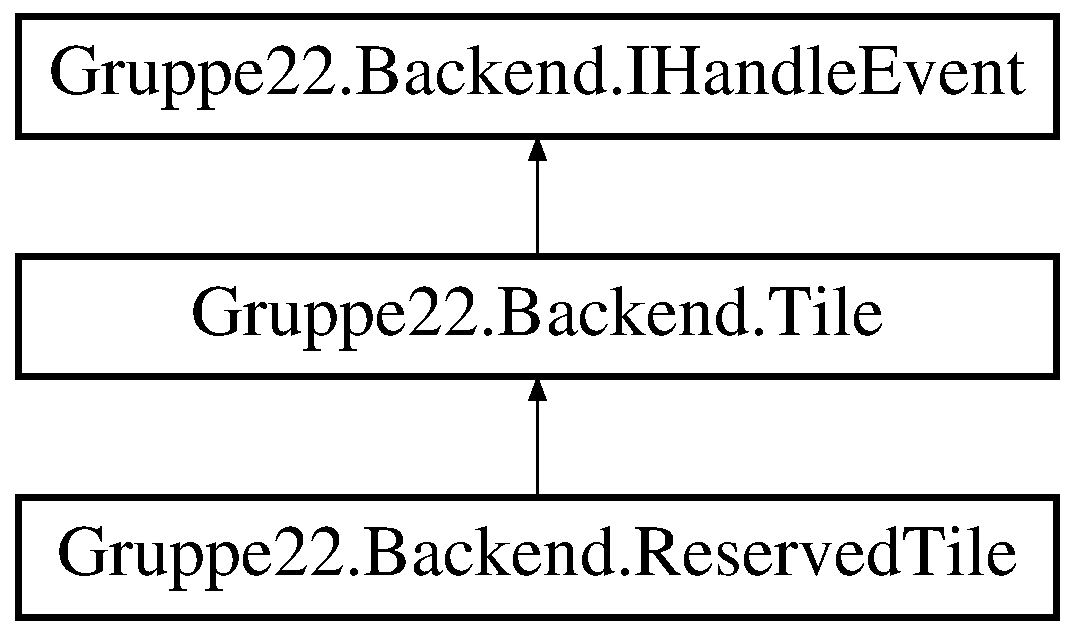
\includegraphics[height=3.000000cm]{class_gruppe22_1_1_backend_1_1_reserved_tile}
\end{center}
\end{figure}
\subsection*{Öffentliche Methoden}
\begin{DoxyCompactItemize}
\item 
\hyperlink{class_gruppe22_1_1_backend_1_1_reserved_tile_a6b513ca0ef7f2ba3dab5465d05da3a31}{Reserved\-Tile} (object \hyperlink{class_gruppe22_1_1_backend_1_1_tile_abc12933c70eb3a2ebbb2fde9f45c2632}{parent}, string \hyperlink{class_gruppe22_1_1_backend_1_1_reserved_tile_a0b9d3bb08fee1ff6f97fc261f11ad8e2}{filename}=\char`\"{}\char`\"{}, int \hyperlink{class_gruppe22_1_1_backend_1_1_reserved_tile_a2f29d3692af2bcd57de9c4e258412d5c}{index}=0, bool canenter=false, bool \hyperlink{class_gruppe22_1_1_backend_1_1_reserved_tile_a2335635e0d117d2ddce9490a21b14639}{enabled}=true)
\item 
override void \hyperlink{class_gruppe22_1_1_backend_1_1_reserved_tile_a394fda5eebd1e5c853c904979bbe04ea}{Save} (Xml\-Writer xmlw)
\begin{DoxyCompactList}\small\item\em Abstract method to save a tile in a X\-M\-L file \end{DoxyCompactList}\end{DoxyCompactItemize}
\subsection*{Propertys}
\begin{DoxyCompactItemize}
\item 
int \hyperlink{class_gruppe22_1_1_backend_1_1_reserved_tile_aff2b70555e9daf0af4ed1b5993e5e05d}{env\-Index}\hspace{0.3cm}{\ttfamily  \mbox{[}get, set\mbox{]}}
\item 
bool \hyperlink{class_gruppe22_1_1_backend_1_1_reserved_tile_a2335635e0d117d2ddce9490a21b14639}{enabled}\hspace{0.3cm}{\ttfamily  \mbox{[}get, set\mbox{]}}
\item 
bool \hyperlink{class_gruppe22_1_1_backend_1_1_reserved_tile_a6fa27616ff1c69df72afb6e341ef1a0d}{can\-Enter}\hspace{0.3cm}{\ttfamily  \mbox{[}get, set\mbox{]}}
\item 
string \hyperlink{class_gruppe22_1_1_backend_1_1_reserved_tile_a0b9d3bb08fee1ff6f97fc261f11ad8e2}{filename}\hspace{0.3cm}{\ttfamily  \mbox{[}get, set\mbox{]}}
\item 
int \hyperlink{class_gruppe22_1_1_backend_1_1_reserved_tile_a2f29d3692af2bcd57de9c4e258412d5c}{index}\hspace{0.3cm}{\ttfamily  \mbox{[}get, set\mbox{]}}
\end{DoxyCompactItemize}
\subsection*{Weitere Geerbte Elemente}


\subsection{Beschreibung der Konstruktoren und Destruktoren}
\hypertarget{class_gruppe22_1_1_backend_1_1_reserved_tile_a6b513ca0ef7f2ba3dab5465d05da3a31}{\index{Gruppe22\-::\-Backend\-::\-Reserved\-Tile@{Gruppe22\-::\-Backend\-::\-Reserved\-Tile}!Reserved\-Tile@{Reserved\-Tile}}
\index{Reserved\-Tile@{Reserved\-Tile}!Gruppe22::Backend::ReservedTile@{Gruppe22\-::\-Backend\-::\-Reserved\-Tile}}
\subsubsection[{Reserved\-Tile}]{\setlength{\rightskip}{0pt plus 5cm}Gruppe22.\-Backend.\-Reserved\-Tile.\-Reserved\-Tile (
\begin{DoxyParamCaption}
\item[{object}]{parent, }
\item[{string}]{filename = {\ttfamily \char`\"{}\char`\"{}}, }
\item[{int}]{index = {\ttfamily 0}, }
\item[{bool}]{canenter = {\ttfamily false}, }
\item[{bool}]{enabled = {\ttfamily true}}
\end{DoxyParamCaption}
)}}\label{class_gruppe22_1_1_backend_1_1_reserved_tile_a6b513ca0ef7f2ba3dab5465d05da3a31}


\subsection{Dokumentation der Elementfunktionen}
\hypertarget{class_gruppe22_1_1_backend_1_1_reserved_tile_a394fda5eebd1e5c853c904979bbe04ea}{\index{Gruppe22\-::\-Backend\-::\-Reserved\-Tile@{Gruppe22\-::\-Backend\-::\-Reserved\-Tile}!Save@{Save}}
\index{Save@{Save}!Gruppe22::Backend::ReservedTile@{Gruppe22\-::\-Backend\-::\-Reserved\-Tile}}
\subsubsection[{Save}]{\setlength{\rightskip}{0pt plus 5cm}override void Gruppe22.\-Backend.\-Reserved\-Tile.\-Save (
\begin{DoxyParamCaption}
\item[{Xml\-Writer}]{xmlw}
\end{DoxyParamCaption}
)\hspace{0.3cm}{\ttfamily [virtual]}}}\label{class_gruppe22_1_1_backend_1_1_reserved_tile_a394fda5eebd1e5c853c904979bbe04ea}


Abstract method to save a tile in a X\-M\-L file 


\begin{DoxyParams}{Parameter}
{\em xmlw} & the Xml\-Writer used for saving the file\\
\hline
\end{DoxyParams}


Erneute Implementation von \hyperlink{class_gruppe22_1_1_backend_1_1_tile_a109ab3e77ffca9d44c95a711af3491dc}{Gruppe22.\-Backend.\-Tile}.



\subsection{Dokumentation der Propertys}
\hypertarget{class_gruppe22_1_1_backend_1_1_reserved_tile_a6fa27616ff1c69df72afb6e341ef1a0d}{\index{Gruppe22\-::\-Backend\-::\-Reserved\-Tile@{Gruppe22\-::\-Backend\-::\-Reserved\-Tile}!can\-Enter@{can\-Enter}}
\index{can\-Enter@{can\-Enter}!Gruppe22::Backend::ReservedTile@{Gruppe22\-::\-Backend\-::\-Reserved\-Tile}}
\subsubsection[{can\-Enter}]{\setlength{\rightskip}{0pt plus 5cm}bool Gruppe22.\-Backend.\-Reserved\-Tile.\-can\-Enter\hspace{0.3cm}{\ttfamily [get]}, {\ttfamily [set]}}}\label{class_gruppe22_1_1_backend_1_1_reserved_tile_a6fa27616ff1c69df72afb6e341ef1a0d}
\hypertarget{class_gruppe22_1_1_backend_1_1_reserved_tile_a2335635e0d117d2ddce9490a21b14639}{\index{Gruppe22\-::\-Backend\-::\-Reserved\-Tile@{Gruppe22\-::\-Backend\-::\-Reserved\-Tile}!enabled@{enabled}}
\index{enabled@{enabled}!Gruppe22::Backend::ReservedTile@{Gruppe22\-::\-Backend\-::\-Reserved\-Tile}}
\subsubsection[{enabled}]{\setlength{\rightskip}{0pt plus 5cm}bool Gruppe22.\-Backend.\-Reserved\-Tile.\-enabled\hspace{0.3cm}{\ttfamily [get]}, {\ttfamily [set]}}}\label{class_gruppe22_1_1_backend_1_1_reserved_tile_a2335635e0d117d2ddce9490a21b14639}
\hypertarget{class_gruppe22_1_1_backend_1_1_reserved_tile_aff2b70555e9daf0af4ed1b5993e5e05d}{\index{Gruppe22\-::\-Backend\-::\-Reserved\-Tile@{Gruppe22\-::\-Backend\-::\-Reserved\-Tile}!env\-Index@{env\-Index}}
\index{env\-Index@{env\-Index}!Gruppe22::Backend::ReservedTile@{Gruppe22\-::\-Backend\-::\-Reserved\-Tile}}
\subsubsection[{env\-Index}]{\setlength{\rightskip}{0pt plus 5cm}int Gruppe22.\-Backend.\-Reserved\-Tile.\-env\-Index\hspace{0.3cm}{\ttfamily [get]}, {\ttfamily [set]}}}\label{class_gruppe22_1_1_backend_1_1_reserved_tile_aff2b70555e9daf0af4ed1b5993e5e05d}
\hypertarget{class_gruppe22_1_1_backend_1_1_reserved_tile_a0b9d3bb08fee1ff6f97fc261f11ad8e2}{\index{Gruppe22\-::\-Backend\-::\-Reserved\-Tile@{Gruppe22\-::\-Backend\-::\-Reserved\-Tile}!filename@{filename}}
\index{filename@{filename}!Gruppe22::Backend::ReservedTile@{Gruppe22\-::\-Backend\-::\-Reserved\-Tile}}
\subsubsection[{filename}]{\setlength{\rightskip}{0pt plus 5cm}string Gruppe22.\-Backend.\-Reserved\-Tile.\-filename\hspace{0.3cm}{\ttfamily [get]}, {\ttfamily [set]}}}\label{class_gruppe22_1_1_backend_1_1_reserved_tile_a0b9d3bb08fee1ff6f97fc261f11ad8e2}
\hypertarget{class_gruppe22_1_1_backend_1_1_reserved_tile_a2f29d3692af2bcd57de9c4e258412d5c}{\index{Gruppe22\-::\-Backend\-::\-Reserved\-Tile@{Gruppe22\-::\-Backend\-::\-Reserved\-Tile}!index@{index}}
\index{index@{index}!Gruppe22::Backend::ReservedTile@{Gruppe22\-::\-Backend\-::\-Reserved\-Tile}}
\subsubsection[{index}]{\setlength{\rightskip}{0pt plus 5cm}int Gruppe22.\-Backend.\-Reserved\-Tile.\-index\hspace{0.3cm}{\ttfamily [get]}, {\ttfamily [set]}}}\label{class_gruppe22_1_1_backend_1_1_reserved_tile_a2f29d3692af2bcd57de9c4e258412d5c}


Die Dokumentation für diese Klasse wurde erzeugt aufgrund der Datei\-:\begin{DoxyCompactItemize}
\item 
C\-:/\-Users/beursken/\-Documents/\-Git\-Hub/gruppe22/\-Gruppe22/\-Gruppe22/\-Backend/\-Map/\hyperlink{_reserved_tile_8cs}{Reserved\-Tile.\-cs}\end{DoxyCompactItemize}

\hypertarget{class_dungeon_server_1_1_server}{\section{Dungeon\-Server.\-Server Klassenreferenz}
\label{class_dungeon_server_1_1_server}\index{Dungeon\-Server.\-Server@{Dungeon\-Server.\-Server}}
}


This class represents the main console application Current version copied almost verbatim from \href{http://www.indiedev.de/wiki/Netzwerk-Basics_mit_Lidgren/Erstellen_des_Servers}{\tt http\-://www.\-indiedev.\-de/wiki/\-Netzwerk-\/\-Basics\-\_\-mit\-\_\-\-Lidgren/\-Erstellen\-\_\-des\-\_\-\-Servers}  


\subsection*{Öffentliche, statische Methoden}
\begin{DoxyCompactItemize}
\item 
static void \hyperlink{class_dungeon_server_1_1_server_a54c03c2317e2da26f8bd641ba71360f2}{Main} (string\mbox{[}$\,$\mbox{]} args)
\begin{DoxyCompactList}\small\item\em Main method \end{DoxyCompactList}\end{DoxyCompactItemize}


\subsection{Ausführliche Beschreibung}
This class represents the main console application Current version copied almost verbatim from \href{http://www.indiedev.de/wiki/Netzwerk-Basics_mit_Lidgren/Erstellen_des_Servers}{\tt http\-://www.\-indiedev.\-de/wiki/\-Netzwerk-\/\-Basics\-\_\-mit\-\_\-\-Lidgren/\-Erstellen\-\_\-des\-\_\-\-Servers} 



\subsection{Dokumentation der Elementfunktionen}
\hypertarget{class_dungeon_server_1_1_server_a54c03c2317e2da26f8bd641ba71360f2}{\index{Dungeon\-Server\-::\-Server@{Dungeon\-Server\-::\-Server}!Main@{Main}}
\index{Main@{Main}!DungeonServer::Server@{Dungeon\-Server\-::\-Server}}
\subsubsection[{Main}]{\setlength{\rightskip}{0pt plus 5cm}static void Dungeon\-Server.\-Server.\-Main (
\begin{DoxyParamCaption}
\item[{string\mbox{[}$\,$\mbox{]}}]{args}
\end{DoxyParamCaption}
)\hspace{0.3cm}{\ttfamily [static]}}}\label{class_dungeon_server_1_1_server_a54c03c2317e2da26f8bd641ba71360f2}


Main method 


\begin{DoxyParams}{Parameter}
{\em args} & \\
\hline
\end{DoxyParams}


Die Dokumentation für diese Klasse wurde erzeugt aufgrund der Datei\-:\begin{DoxyCompactItemize}
\item 
C\-:/\-Users/beursken/\-Documents/\-Git\-Hub/gruppe22/\-Gruppe22/\-Dungeon\-Server/\hyperlink{_dungeon_server_2_program_8cs}{Program.\-cs}\end{DoxyCompactItemize}

\hypertarget{class_gruppe22_1_1_client_1_1_shop}{\section{Gruppe22.\-Client.\-Shop Klassenreferenz}
\label{class_gruppe22_1_1_client_1_1_shop}\index{Gruppe22.\-Client.\-Shop@{Gruppe22.\-Client.\-Shop}}
}
Klassendiagramm für Gruppe22.\-Client.\-Shop\-:\begin{figure}[H]
\begin{center}
\leavevmode
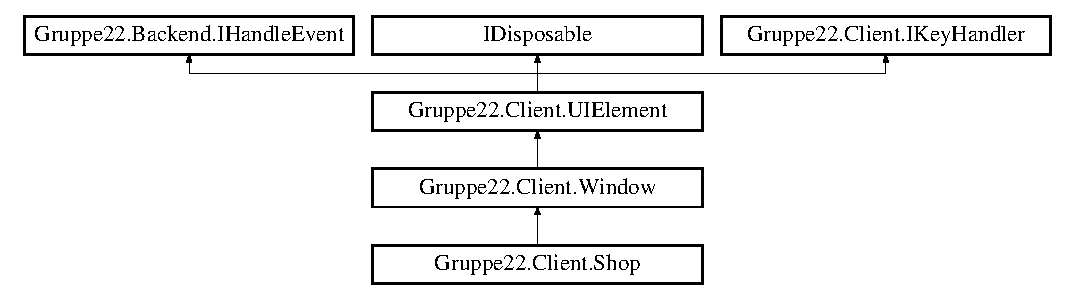
\includegraphics[height=3.589744cm]{class_gruppe22_1_1_client_1_1_shop}
\end{center}
\end{figure}
\subsection*{Öffentliche Methoden}
\begin{DoxyCompactItemize}
\item 
void \hyperlink{class_gruppe22_1_1_client_1_1_shop_a4d05237c2675b7b593417b8ee6f9896b}{Display\-Tool\-Tip} (int column, int y, string text)
\begin{DoxyCompactList}\small\item\em Append a new line of text to the status box; word wrap if necessary \end{DoxyCompactList}\item 
override void \hyperlink{class_gruppe22_1_1_client_1_1_shop_ade0a07f29b074538cafdd5dedabc906b}{Draw} (Game\-Time game\-Time)
\item 
override void \hyperlink{class_gruppe22_1_1_client_1_1_shop_acb19ef7e140c9eb1a873cb0178e7aae3}{Update} (Game\-Time game\-Time)
\item 
override bool \hyperlink{class_gruppe22_1_1_client_1_1_shop_a38e6f534bd8c651103d61bcee914f60e}{On\-Mouse\-Down} (int button)
\begin{DoxyCompactList}\small\item\em Called when a mouse button changes from up to down \end{DoxyCompactList}\item 
override bool \hyperlink{class_gruppe22_1_1_client_1_1_shop_ad56f17fd523aa1984251aded8e00a8d3}{On\-Key\-Down} (Microsoft.\-Xna.\-Framework.\-Input.\-Keys k)
\item 
override void \hyperlink{class_gruppe22_1_1_client_1_1_shop_a940b015eb2925298e2c80571ae4bfe15}{Handle\-Event} (bool Down\-Stream, \hyperlink{namespace_gruppe22_1_1_backend_ab56df91bb0bdafa1ea978e552209ce73}{Backend.\-Events} event\-I\-D, params object\mbox{[}$\,$\mbox{]} data)
\item 
\hyperlink{class_gruppe22_1_1_client_1_1_shop_a547d78600127bdd96b2058c952186599}{Shop} (\hyperlink{interface_gruppe22_1_1_backend_1_1_i_handle_event}{Backend.\-I\-Handle\-Event} parent, Sprite\-Batch sprite\-Batch, Content\-Manager content, Rectangle display\-Rect, \hyperlink{class_gruppe22_1_1_backend_1_1_actor}{Backend.\-Actor} actor1, \hyperlink{class_gruppe22_1_1_backend_1_1_actor}{Backend.\-Actor} actor2)
\begin{DoxyCompactList}\small\item\em Constructor \end{DoxyCompactList}\end{DoxyCompactItemize}
\subsection*{Weitere Geerbte Elemente}


\subsection{Beschreibung der Konstruktoren und Destruktoren}
\hypertarget{class_gruppe22_1_1_client_1_1_shop_a547d78600127bdd96b2058c952186599}{\index{Gruppe22\-::\-Client\-::\-Shop@{Gruppe22\-::\-Client\-::\-Shop}!Shop@{Shop}}
\index{Shop@{Shop}!Gruppe22::Client::Shop@{Gruppe22\-::\-Client\-::\-Shop}}
\subsubsection[{Shop}]{\setlength{\rightskip}{0pt plus 5cm}Gruppe22.\-Client.\-Shop.\-Shop (
\begin{DoxyParamCaption}
\item[{{\bf Backend.\-I\-Handle\-Event}}]{parent, }
\item[{Sprite\-Batch}]{sprite\-Batch, }
\item[{Content\-Manager}]{content, }
\item[{Rectangle}]{display\-Rect, }
\item[{{\bf Backend.\-Actor}}]{actor1, }
\item[{{\bf Backend.\-Actor}}]{actor2}
\end{DoxyParamCaption}
)}}\label{class_gruppe22_1_1_client_1_1_shop_a547d78600127bdd96b2058c952186599}


Constructor 



\subsection{Dokumentation der Elementfunktionen}
\hypertarget{class_gruppe22_1_1_client_1_1_shop_a4d05237c2675b7b593417b8ee6f9896b}{\index{Gruppe22\-::\-Client\-::\-Shop@{Gruppe22\-::\-Client\-::\-Shop}!Display\-Tool\-Tip@{Display\-Tool\-Tip}}
\index{Display\-Tool\-Tip@{Display\-Tool\-Tip}!Gruppe22::Client::Shop@{Gruppe22\-::\-Client\-::\-Shop}}
\subsubsection[{Display\-Tool\-Tip}]{\setlength{\rightskip}{0pt plus 5cm}void Gruppe22.\-Client.\-Shop.\-Display\-Tool\-Tip (
\begin{DoxyParamCaption}
\item[{int}]{column, }
\item[{int}]{y, }
\item[{string}]{text}
\end{DoxyParamCaption}
)}}\label{class_gruppe22_1_1_client_1_1_shop_a4d05237c2675b7b593417b8ee6f9896b}


Append a new line of text to the status box; word wrap if necessary 


\begin{DoxyParams}{Parameter}
{\em text} & \\
\hline
\end{DoxyParams}
\hypertarget{class_gruppe22_1_1_client_1_1_shop_ade0a07f29b074538cafdd5dedabc906b}{\index{Gruppe22\-::\-Client\-::\-Shop@{Gruppe22\-::\-Client\-::\-Shop}!Draw@{Draw}}
\index{Draw@{Draw}!Gruppe22::Client::Shop@{Gruppe22\-::\-Client\-::\-Shop}}
\subsubsection[{Draw}]{\setlength{\rightskip}{0pt plus 5cm}override void Gruppe22.\-Client.\-Shop.\-Draw (
\begin{DoxyParamCaption}
\item[{Game\-Time}]{game\-Time}
\end{DoxyParamCaption}
)\hspace{0.3cm}{\ttfamily [virtual]}}}\label{class_gruppe22_1_1_client_1_1_shop_ade0a07f29b074538cafdd5dedabc906b}





\begin{DoxyParams}{Parameter}
{\em game\-Time} & \\
\hline
\end{DoxyParams}


Erneute Implementation von \hyperlink{class_gruppe22_1_1_client_1_1_u_i_element_ae68afcbd1db3540052d6b399022e56e7}{Gruppe22.\-Client.\-U\-I\-Element}.

\hypertarget{class_gruppe22_1_1_client_1_1_shop_a940b015eb2925298e2c80571ae4bfe15}{\index{Gruppe22\-::\-Client\-::\-Shop@{Gruppe22\-::\-Client\-::\-Shop}!Handle\-Event@{Handle\-Event}}
\index{Handle\-Event@{Handle\-Event}!Gruppe22::Client::Shop@{Gruppe22\-::\-Client\-::\-Shop}}
\subsubsection[{Handle\-Event}]{\setlength{\rightskip}{0pt plus 5cm}override void Gruppe22.\-Client.\-Shop.\-Handle\-Event (
\begin{DoxyParamCaption}
\item[{bool}]{Down\-Stream, }
\item[{{\bf Backend.\-Events}}]{event\-I\-D, }
\item[{params object\mbox{[}$\,$\mbox{]}}]{data}
\end{DoxyParamCaption}
)\hspace{0.3cm}{\ttfamily [virtual]}}}\label{class_gruppe22_1_1_client_1_1_shop_a940b015eb2925298e2c80571ae4bfe15}


Erneute Implementation von \hyperlink{class_gruppe22_1_1_client_1_1_u_i_element_ad06a1ce6c1705a1c7aa91756f368a517}{Gruppe22.\-Client.\-U\-I\-Element}.

\hypertarget{class_gruppe22_1_1_client_1_1_shop_ad56f17fd523aa1984251aded8e00a8d3}{\index{Gruppe22\-::\-Client\-::\-Shop@{Gruppe22\-::\-Client\-::\-Shop}!On\-Key\-Down@{On\-Key\-Down}}
\index{On\-Key\-Down@{On\-Key\-Down}!Gruppe22::Client::Shop@{Gruppe22\-::\-Client\-::\-Shop}}
\subsubsection[{On\-Key\-Down}]{\setlength{\rightskip}{0pt plus 5cm}override bool Gruppe22.\-Client.\-Shop.\-On\-Key\-Down (
\begin{DoxyParamCaption}
\item[{Microsoft.\-Xna.\-Framework.\-Input.\-Keys}]{k}
\end{DoxyParamCaption}
)}}\label{class_gruppe22_1_1_client_1_1_shop_ad56f17fd523aa1984251aded8e00a8d3}
\hypertarget{class_gruppe22_1_1_client_1_1_shop_a38e6f534bd8c651103d61bcee914f60e}{\index{Gruppe22\-::\-Client\-::\-Shop@{Gruppe22\-::\-Client\-::\-Shop}!On\-Mouse\-Down@{On\-Mouse\-Down}}
\index{On\-Mouse\-Down@{On\-Mouse\-Down}!Gruppe22::Client::Shop@{Gruppe22\-::\-Client\-::\-Shop}}
\subsubsection[{On\-Mouse\-Down}]{\setlength{\rightskip}{0pt plus 5cm}override bool Gruppe22.\-Client.\-Shop.\-On\-Mouse\-Down (
\begin{DoxyParamCaption}
\item[{int}]{button}
\end{DoxyParamCaption}
)\hspace{0.3cm}{\ttfamily [virtual]}}}\label{class_gruppe22_1_1_client_1_1_shop_a38e6f534bd8c651103d61bcee914f60e}


Called when a mouse button changes from up to down 


\begin{DoxyParams}{Parameter}
{\em button} & Left \hyperlink{class_gruppe22_1_1_client_1_1_button}{Button}=1, Middle \hyperlink{class_gruppe22_1_1_client_1_1_button}{Button}=2, Right \hyperlink{class_gruppe22_1_1_client_1_1_button}{Button}=3\\
\hline
\end{DoxyParams}


Erneute Implementation von \hyperlink{class_gruppe22_1_1_client_1_1_u_i_element_a0530df2286336160b8b39c74ba380a44}{Gruppe22.\-Client.\-U\-I\-Element}.

\hypertarget{class_gruppe22_1_1_client_1_1_shop_acb19ef7e140c9eb1a873cb0178e7aae3}{\index{Gruppe22\-::\-Client\-::\-Shop@{Gruppe22\-::\-Client\-::\-Shop}!Update@{Update}}
\index{Update@{Update}!Gruppe22::Client::Shop@{Gruppe22\-::\-Client\-::\-Shop}}
\subsubsection[{Update}]{\setlength{\rightskip}{0pt plus 5cm}override void Gruppe22.\-Client.\-Shop.\-Update (
\begin{DoxyParamCaption}
\item[{Game\-Time}]{game\-Time}
\end{DoxyParamCaption}
)\hspace{0.3cm}{\ttfamily [virtual]}}}\label{class_gruppe22_1_1_client_1_1_shop_acb19ef7e140c9eb1a873cb0178e7aae3}





\begin{DoxyParams}{Parameter}
{\em game\-Time} & \\
\hline
\end{DoxyParams}


Erneute Implementation von \hyperlink{class_gruppe22_1_1_client_1_1_u_i_element_a456bc763b6ed6ab441bb0ae96b6f4f8b}{Gruppe22.\-Client.\-U\-I\-Element}.



Die Dokumentation für diese Klasse wurde erzeugt aufgrund der Datei\-:\begin{DoxyCompactItemize}
\item 
C\-:/\-Users/beursken/\-Documents/\-Git\-Hub/gruppe22/\-Gruppe22/\-Gruppe22/\-Client/\-U\-I/\hyperlink{_shop_8cs}{Shop.\-cs}\end{DoxyCompactItemize}

\hypertarget{class_gruppe22_1_1_client_1_1_simple_stats}{\section{Gruppe22.\-Client.\-Simple\-Stats Klassenreferenz}
\label{class_gruppe22_1_1_client_1_1_simple_stats}\index{Gruppe22.\-Client.\-Simple\-Stats@{Gruppe22.\-Client.\-Simple\-Stats}}
}
Klassendiagramm für Gruppe22.\-Client.\-Simple\-Stats\-:\begin{figure}[H]
\begin{center}
\leavevmode
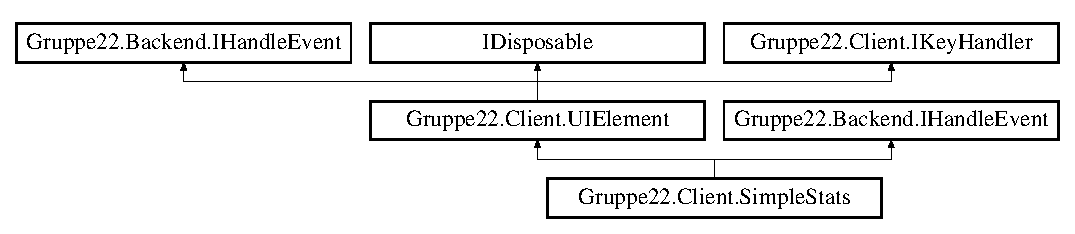
\includegraphics[height=2.692308cm]{class_gruppe22_1_1_client_1_1_simple_stats}
\end{center}
\end{figure}
\subsection*{Öffentliche Methoden}
\begin{DoxyCompactItemize}
\item 
override bool \hyperlink{class_gruppe22_1_1_client_1_1_simple_stats_adef63cea6f4c63a0d9b8c6a07b54a871}{On\-Mouse\-Down} (int button)
\begin{DoxyCompactList}\small\item\em Called when a mouse button changes from up to down \end{DoxyCompactList}\item 
override void \hyperlink{class_gruppe22_1_1_client_1_1_simple_stats_a2caae8c55a4ddde3fd3605d980d6cdaa}{Update} (Game\-Time game\-Time)
\begin{DoxyCompactList}\small\item\em React to changes in character stats \end{DoxyCompactList}\item 
override void \hyperlink{class_gruppe22_1_1_client_1_1_simple_stats_a3fcb27fbe6cf2fce3c6fe4215de147d2}{Draw} (Game\-Time game\-Time)
\begin{DoxyCompactList}\small\item\em Refresh display of actor data \end{DoxyCompactList}\item 
\hyperlink{class_gruppe22_1_1_client_1_1_simple_stats_a5a8d67799cbb72eb3208eb92990e7279}{Simple\-Stats} (\hyperlink{interface_gruppe22_1_1_backend_1_1_i_handle_event}{Backend.\-I\-Handle\-Event} parent, Sprite\-Batch sprite\-Batch, Content\-Manager content, Rectangle display\-Rect, \hyperlink{class_gruppe22_1_1_backend_1_1_actor}{Backend.\-Actor} \hyperlink{class_gruppe22_1_1_client_1_1_simple_stats_a49b12e4d4fc1845f976ea160109663fb}{actor})
\begin{DoxyCompactList}\small\item\em Constructor \end{DoxyCompactList}\end{DoxyCompactItemize}
\subsection*{Propertys}
\begin{DoxyCompactItemize}
\item 
\hyperlink{class_gruppe22_1_1_backend_1_1_actor}{Backend.\-Actor} \hyperlink{class_gruppe22_1_1_client_1_1_simple_stats_a49b12e4d4fc1845f976ea160109663fb}{actor}\hspace{0.3cm}{\ttfamily  \mbox{[}get, set\mbox{]}}
\end{DoxyCompactItemize}
\subsection*{Weitere Geerbte Elemente}


\subsection{Beschreibung der Konstruktoren und Destruktoren}
\hypertarget{class_gruppe22_1_1_client_1_1_simple_stats_a5a8d67799cbb72eb3208eb92990e7279}{\index{Gruppe22\-::\-Client\-::\-Simple\-Stats@{Gruppe22\-::\-Client\-::\-Simple\-Stats}!Simple\-Stats@{Simple\-Stats}}
\index{Simple\-Stats@{Simple\-Stats}!Gruppe22::Client::SimpleStats@{Gruppe22\-::\-Client\-::\-Simple\-Stats}}
\subsubsection[{Simple\-Stats}]{\setlength{\rightskip}{0pt plus 5cm}Gruppe22.\-Client.\-Simple\-Stats.\-Simple\-Stats (
\begin{DoxyParamCaption}
\item[{{\bf Backend.\-I\-Handle\-Event}}]{parent, }
\item[{Sprite\-Batch}]{sprite\-Batch, }
\item[{Content\-Manager}]{content, }
\item[{Rectangle}]{display\-Rect, }
\item[{{\bf Backend.\-Actor}}]{actor}
\end{DoxyParamCaption}
)}}\label{class_gruppe22_1_1_client_1_1_simple_stats_a5a8d67799cbb72eb3208eb92990e7279}


Constructor 



\subsection{Dokumentation der Elementfunktionen}
\hypertarget{class_gruppe22_1_1_client_1_1_simple_stats_a3fcb27fbe6cf2fce3c6fe4215de147d2}{\index{Gruppe22\-::\-Client\-::\-Simple\-Stats@{Gruppe22\-::\-Client\-::\-Simple\-Stats}!Draw@{Draw}}
\index{Draw@{Draw}!Gruppe22::Client::SimpleStats@{Gruppe22\-::\-Client\-::\-Simple\-Stats}}
\subsubsection[{Draw}]{\setlength{\rightskip}{0pt plus 5cm}override void Gruppe22.\-Client.\-Simple\-Stats.\-Draw (
\begin{DoxyParamCaption}
\item[{Game\-Time}]{game\-Time}
\end{DoxyParamCaption}
)\hspace{0.3cm}{\ttfamily [virtual]}}}\label{class_gruppe22_1_1_client_1_1_simple_stats_a3fcb27fbe6cf2fce3c6fe4215de147d2}


Refresh display of actor data 


\begin{DoxyParams}{Parameter}
{\em game\-Time} & Provides a snapshot of timing values.\\
\hline
\end{DoxyParams}


Erneute Implementation von \hyperlink{class_gruppe22_1_1_client_1_1_u_i_element_ae68afcbd1db3540052d6b399022e56e7}{Gruppe22.\-Client.\-U\-I\-Element}.

\hypertarget{class_gruppe22_1_1_client_1_1_simple_stats_adef63cea6f4c63a0d9b8c6a07b54a871}{\index{Gruppe22\-::\-Client\-::\-Simple\-Stats@{Gruppe22\-::\-Client\-::\-Simple\-Stats}!On\-Mouse\-Down@{On\-Mouse\-Down}}
\index{On\-Mouse\-Down@{On\-Mouse\-Down}!Gruppe22::Client::SimpleStats@{Gruppe22\-::\-Client\-::\-Simple\-Stats}}
\subsubsection[{On\-Mouse\-Down}]{\setlength{\rightskip}{0pt plus 5cm}override bool Gruppe22.\-Client.\-Simple\-Stats.\-On\-Mouse\-Down (
\begin{DoxyParamCaption}
\item[{int}]{button}
\end{DoxyParamCaption}
)\hspace{0.3cm}{\ttfamily [virtual]}}}\label{class_gruppe22_1_1_client_1_1_simple_stats_adef63cea6f4c63a0d9b8c6a07b54a871}


Called when a mouse button changes from up to down 


\begin{DoxyParams}{Parameter}
{\em button} & Left \hyperlink{class_gruppe22_1_1_client_1_1_button}{Button}=1, Middle \hyperlink{class_gruppe22_1_1_client_1_1_button}{Button}=2, Right \hyperlink{class_gruppe22_1_1_client_1_1_button}{Button}=3\\
\hline
\end{DoxyParams}


Erneute Implementation von \hyperlink{class_gruppe22_1_1_client_1_1_u_i_element_a0530df2286336160b8b39c74ba380a44}{Gruppe22.\-Client.\-U\-I\-Element}.

\hypertarget{class_gruppe22_1_1_client_1_1_simple_stats_a2caae8c55a4ddde3fd3605d980d6cdaa}{\index{Gruppe22\-::\-Client\-::\-Simple\-Stats@{Gruppe22\-::\-Client\-::\-Simple\-Stats}!Update@{Update}}
\index{Update@{Update}!Gruppe22::Client::SimpleStats@{Gruppe22\-::\-Client\-::\-Simple\-Stats}}
\subsubsection[{Update}]{\setlength{\rightskip}{0pt plus 5cm}override void Gruppe22.\-Client.\-Simple\-Stats.\-Update (
\begin{DoxyParamCaption}
\item[{Game\-Time}]{game\-Time}
\end{DoxyParamCaption}
)\hspace{0.3cm}{\ttfamily [virtual]}}}\label{class_gruppe22_1_1_client_1_1_simple_stats_a2caae8c55a4ddde3fd3605d980d6cdaa}


React to changes in character stats 


\begin{DoxyParams}{Parameter}
{\em game\-Time} & \\
\hline
\end{DoxyParams}


Erneute Implementation von \hyperlink{class_gruppe22_1_1_client_1_1_u_i_element_a456bc763b6ed6ab441bb0ae96b6f4f8b}{Gruppe22.\-Client.\-U\-I\-Element}.



\subsection{Dokumentation der Propertys}
\hypertarget{class_gruppe22_1_1_client_1_1_simple_stats_a49b12e4d4fc1845f976ea160109663fb}{\index{Gruppe22\-::\-Client\-::\-Simple\-Stats@{Gruppe22\-::\-Client\-::\-Simple\-Stats}!actor@{actor}}
\index{actor@{actor}!Gruppe22::Client::SimpleStats@{Gruppe22\-::\-Client\-::\-Simple\-Stats}}
\subsubsection[{actor}]{\setlength{\rightskip}{0pt plus 5cm}{\bf Backend.\-Actor} Gruppe22.\-Client.\-Simple\-Stats.\-actor\hspace{0.3cm}{\ttfamily [get]}, {\ttfamily [set]}}}\label{class_gruppe22_1_1_client_1_1_simple_stats_a49b12e4d4fc1845f976ea160109663fb}


Die Dokumentation für diese Klasse wurde erzeugt aufgrund der Datei\-:\begin{DoxyCompactItemize}
\item 
C\-:/\-Users/beursken/\-Documents/\-Git\-Hub/gruppe22/\-Gruppe22/\-Gruppe22/\-Client/\-U\-I/\hyperlink{_simple_stats_8cs}{Simple\-Stats.\-cs}\end{DoxyCompactItemize}

\hypertarget{class_gruppe22_1_1_client_1_1_state_to_event}{\section{Gruppe22.\-Client.\-State\-To\-Event Klassenreferenz}
\label{class_gruppe22_1_1_client_1_1_state_to_event}\index{Gruppe22.\-Client.\-State\-To\-Event@{Gruppe22.\-Client.\-State\-To\-Event}}
}


A class transforming mouse and keyboard-\/states to Windows Forms style events  


\subsection*{Öffentliche Methoden}
\begin{DoxyCompactItemize}
\item 
void \hyperlink{class_gruppe22_1_1_client_1_1_state_to_event_a5dda91539d198a68342ab92d123a1f89}{Update} (Game\-Time gametime)
\begin{DoxyCompactList}\small\item\em Change states and pass events if needed \end{DoxyCompactList}\item 
\hyperlink{class_gruppe22_1_1_client_1_1_state_to_event_ab5a1f526f0001a8159baf1390d4e6ad8}{State\-To\-Event} (\hyperlink{interface_gruppe22_1_1_client_1_1_i_key_handler}{I\-Key\-Handler} parent)
\begin{DoxyCompactList}\small\item\em Create a new State to event transformer (possibly only for mainwindow) \end{DoxyCompactList}\end{DoxyCompactItemize}
\subsection*{Propertys}
\begin{DoxyCompactItemize}
\item 
Keys\mbox{[}$\,$\mbox{]} \hyperlink{class_gruppe22_1_1_client_1_1_state_to_event_a65989c04116808478b150febeeb9f8b6}{keys}\hspace{0.3cm}{\ttfamily  \mbox{[}get\mbox{]}}
\end{DoxyCompactItemize}


\subsection{Ausführliche Beschreibung}
A class transforming mouse and keyboard-\/states to Windows Forms style events 



\subsection{Beschreibung der Konstruktoren und Destruktoren}
\hypertarget{class_gruppe22_1_1_client_1_1_state_to_event_ab5a1f526f0001a8159baf1390d4e6ad8}{\index{Gruppe22\-::\-Client\-::\-State\-To\-Event@{Gruppe22\-::\-Client\-::\-State\-To\-Event}!State\-To\-Event@{State\-To\-Event}}
\index{State\-To\-Event@{State\-To\-Event}!Gruppe22::Client::StateToEvent@{Gruppe22\-::\-Client\-::\-State\-To\-Event}}
\subsubsection[{State\-To\-Event}]{\setlength{\rightskip}{0pt plus 5cm}Gruppe22.\-Client.\-State\-To\-Event.\-State\-To\-Event (
\begin{DoxyParamCaption}
\item[{{\bf I\-Key\-Handler}}]{parent}
\end{DoxyParamCaption}
)}}\label{class_gruppe22_1_1_client_1_1_state_to_event_ab5a1f526f0001a8159baf1390d4e6ad8}


Create a new State to event transformer (possibly only for mainwindow) 


\begin{DoxyParams}{Parameter}
{\em parent} & \\
\hline
\end{DoxyParams}


\subsection{Dokumentation der Elementfunktionen}
\hypertarget{class_gruppe22_1_1_client_1_1_state_to_event_a5dda91539d198a68342ab92d123a1f89}{\index{Gruppe22\-::\-Client\-::\-State\-To\-Event@{Gruppe22\-::\-Client\-::\-State\-To\-Event}!Update@{Update}}
\index{Update@{Update}!Gruppe22::Client::StateToEvent@{Gruppe22\-::\-Client\-::\-State\-To\-Event}}
\subsubsection[{Update}]{\setlength{\rightskip}{0pt plus 5cm}void Gruppe22.\-Client.\-State\-To\-Event.\-Update (
\begin{DoxyParamCaption}
\item[{Game\-Time}]{gametime}
\end{DoxyParamCaption}
)}}\label{class_gruppe22_1_1_client_1_1_state_to_event_a5dda91539d198a68342ab92d123a1f89}


Change states and pass events if needed 


\begin{DoxyParams}{Parameter}
{\em gametime} & \\
\hline
\end{DoxyParams}


\subsection{Dokumentation der Propertys}
\hypertarget{class_gruppe22_1_1_client_1_1_state_to_event_a65989c04116808478b150febeeb9f8b6}{\index{Gruppe22\-::\-Client\-::\-State\-To\-Event@{Gruppe22\-::\-Client\-::\-State\-To\-Event}!keys@{keys}}
\index{keys@{keys}!Gruppe22::Client::StateToEvent@{Gruppe22\-::\-Client\-::\-State\-To\-Event}}
\subsubsection[{keys}]{\setlength{\rightskip}{0pt plus 5cm}Keys \mbox{[}$\,$\mbox{]} Gruppe22.\-Client.\-State\-To\-Event.\-keys\hspace{0.3cm}{\ttfamily [get]}}}\label{class_gruppe22_1_1_client_1_1_state_to_event_a65989c04116808478b150febeeb9f8b6}


Die Dokumentation für diese Klasse wurde erzeugt aufgrund der Datei\-:\begin{DoxyCompactItemize}
\item 
C\-:/\-Users/beursken/\-Documents/\-Git\-Hub/gruppe22/\-Gruppe22/\-Gruppe22/\-Client/\-U\-I/\hyperlink{_key_handler_8cs}{Key\-Handler.\-cs}\end{DoxyCompactItemize}

\hypertarget{class_gruppe22_1_1_client_1_1_statusbox}{\section{Gruppe22.\-Client.\-Statusbox Klassenreferenz}
\label{class_gruppe22_1_1_client_1_1_statusbox}\index{Gruppe22.\-Client.\-Statusbox@{Gruppe22.\-Client.\-Statusbox}}
}
Klassendiagramm für Gruppe22.\-Client.\-Statusbox\-:\begin{figure}[H]
\begin{center}
\leavevmode
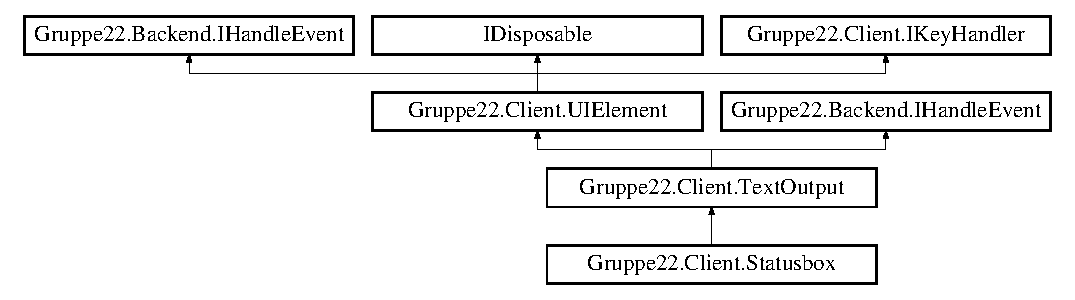
\includegraphics[height=3.589744cm]{class_gruppe22_1_1_client_1_1_statusbox}
\end{center}
\end{figure}
\subsection*{Öffentliche Methoden}
\begin{DoxyCompactItemize}
\item 
override void \hyperlink{class_gruppe22_1_1_client_1_1_statusbox_a5b23e66c24de79d0a274577d63a6ad74}{Add\-Line} (string text, object color=null)
\begin{DoxyCompactList}\small\item\em Append a new line of text to the status box; word wrap if necessary \end{DoxyCompactList}\item 
override void \hyperlink{class_gruppe22_1_1_client_1_1_statusbox_a545d945221658c0c1b348c5fd4b26a69}{Handle\-Event} (bool Down\-Stream, \hyperlink{namespace_gruppe22_1_1_backend_ab56df91bb0bdafa1ea978e552209ce73}{Backend.\-Events} event\-I\-D, params object\mbox{[}$\,$\mbox{]} data)
\item 
override void \hyperlink{class_gruppe22_1_1_client_1_1_statusbox_aa7965174de723d0fc0e8a8f7bbc3be85}{Draw} (Game\-Time game\-Time)
\begin{DoxyCompactList}\small\item\em This is called when the game should draw itself. \end{DoxyCompactList}\item 
override bool \hyperlink{class_gruppe22_1_1_client_1_1_statusbox_ab8eaff6863d543e251756c0954fe193d}{On\-Mouse\-Down} (int button)
\begin{DoxyCompactList}\small\item\em Called when a mouse button changes from up to down \end{DoxyCompactList}\item 
override void \hyperlink{class_gruppe22_1_1_client_1_1_statusbox_a4945809df0ff23018b197049abd420a0}{Move\-Content} (Vector2 difference, int \-\_\-last\-Check=0)
\item 
override void \hyperlink{class_gruppe22_1_1_client_1_1_statusbox_aefcb1642cf6576b9efcdcaaa64f6a879}{Scroll\-Wheel} (int Difference)
\item 
override bool \hyperlink{class_gruppe22_1_1_client_1_1_statusbox_a92512ba8bfcfeb6c417eedf5f1b3634e}{On\-Key\-Down} (Keys k)
\item 
\hyperlink{class_gruppe22_1_1_client_1_1_statusbox_af6dd356420111c04c1110e770ed98727}{Statusbox} (\hyperlink{interface_gruppe22_1_1_backend_1_1_i_handle_event}{Backend.\-I\-Handle\-Event} parent, Sprite\-Batch sprite\-Batch, Content\-Manager content, Rectangle display\-Rect, bool has\-Border=true, bool center=false)
\begin{DoxyCompactList}\small\item\em Creates a scrollable area to output text \end{DoxyCompactList}\end{DoxyCompactItemize}
\subsection*{Weitere Geerbte Elemente}


\subsection{Beschreibung der Konstruktoren und Destruktoren}
\hypertarget{class_gruppe22_1_1_client_1_1_statusbox_af6dd356420111c04c1110e770ed98727}{\index{Gruppe22\-::\-Client\-::\-Statusbox@{Gruppe22\-::\-Client\-::\-Statusbox}!Statusbox@{Statusbox}}
\index{Statusbox@{Statusbox}!Gruppe22::Client::Statusbox@{Gruppe22\-::\-Client\-::\-Statusbox}}
\subsubsection[{Statusbox}]{\setlength{\rightskip}{0pt plus 5cm}Gruppe22.\-Client.\-Statusbox.\-Statusbox (
\begin{DoxyParamCaption}
\item[{{\bf Backend.\-I\-Handle\-Event}}]{parent, }
\item[{Sprite\-Batch}]{sprite\-Batch, }
\item[{Content\-Manager}]{content, }
\item[{Rectangle}]{display\-Rect, }
\item[{bool}]{has\-Border = {\ttfamily true}, }
\item[{bool}]{center = {\ttfamily false}}
\end{DoxyParamCaption}
)}}\label{class_gruppe22_1_1_client_1_1_statusbox_af6dd356420111c04c1110e770ed98727}


Creates a scrollable area to output text 


\begin{DoxyParams}{Parameter}
{\em parent} & \\
\hline
{\em sprite\-Batch} & \\
\hline
{\em content} & \\
\hline
{\em display\-Rect} & \\
\hline
{\em has\-Border} & \\
\hline
{\em center} & \\
\hline
\end{DoxyParams}


\subsection{Dokumentation der Elementfunktionen}
\hypertarget{class_gruppe22_1_1_client_1_1_statusbox_a5b23e66c24de79d0a274577d63a6ad74}{\index{Gruppe22\-::\-Client\-::\-Statusbox@{Gruppe22\-::\-Client\-::\-Statusbox}!Add\-Line@{Add\-Line}}
\index{Add\-Line@{Add\-Line}!Gruppe22::Client::Statusbox@{Gruppe22\-::\-Client\-::\-Statusbox}}
\subsubsection[{Add\-Line}]{\setlength{\rightskip}{0pt plus 5cm}override void Gruppe22.\-Client.\-Statusbox.\-Add\-Line (
\begin{DoxyParamCaption}
\item[{string}]{text, }
\item[{object}]{color = {\ttfamily null}}
\end{DoxyParamCaption}
)\hspace{0.3cm}{\ttfamily [virtual]}}}\label{class_gruppe22_1_1_client_1_1_statusbox_a5b23e66c24de79d0a274577d63a6ad74}


Append a new line of text to the status box; word wrap if necessary 


\begin{DoxyParams}{Parameter}
{\em text} & \\
\hline
\end{DoxyParams}


Erneute Implementation von \hyperlink{class_gruppe22_1_1_client_1_1_text_output_a1350976d5c45cef2d5227b5c4e097896}{Gruppe22.\-Client.\-Text\-Output}.

\hypertarget{class_gruppe22_1_1_client_1_1_statusbox_aa7965174de723d0fc0e8a8f7bbc3be85}{\index{Gruppe22\-::\-Client\-::\-Statusbox@{Gruppe22\-::\-Client\-::\-Statusbox}!Draw@{Draw}}
\index{Draw@{Draw}!Gruppe22::Client::Statusbox@{Gruppe22\-::\-Client\-::\-Statusbox}}
\subsubsection[{Draw}]{\setlength{\rightskip}{0pt plus 5cm}override void Gruppe22.\-Client.\-Statusbox.\-Draw (
\begin{DoxyParamCaption}
\item[{Game\-Time}]{game\-Time}
\end{DoxyParamCaption}
)\hspace{0.3cm}{\ttfamily [virtual]}}}\label{class_gruppe22_1_1_client_1_1_statusbox_aa7965174de723d0fc0e8a8f7bbc3be85}


This is called when the game should draw itself. 


\begin{DoxyParams}{Parameter}
{\em game\-Time} & Provides a snapshot of timing values.\\
\hline
\end{DoxyParams}


Erneute Implementation von \hyperlink{class_gruppe22_1_1_client_1_1_u_i_element_ae68afcbd1db3540052d6b399022e56e7}{Gruppe22.\-Client.\-U\-I\-Element}.

\hypertarget{class_gruppe22_1_1_client_1_1_statusbox_a545d945221658c0c1b348c5fd4b26a69}{\index{Gruppe22\-::\-Client\-::\-Statusbox@{Gruppe22\-::\-Client\-::\-Statusbox}!Handle\-Event@{Handle\-Event}}
\index{Handle\-Event@{Handle\-Event}!Gruppe22::Client::Statusbox@{Gruppe22\-::\-Client\-::\-Statusbox}}
\subsubsection[{Handle\-Event}]{\setlength{\rightskip}{0pt plus 5cm}override void Gruppe22.\-Client.\-Statusbox.\-Handle\-Event (
\begin{DoxyParamCaption}
\item[{bool}]{Down\-Stream, }
\item[{{\bf Backend.\-Events}}]{event\-I\-D, }
\item[{params object\mbox{[}$\,$\mbox{]}}]{data}
\end{DoxyParamCaption}
)\hspace{0.3cm}{\ttfamily [virtual]}}}\label{class_gruppe22_1_1_client_1_1_statusbox_a545d945221658c0c1b348c5fd4b26a69}


Erneute Implementation von \hyperlink{class_gruppe22_1_1_client_1_1_u_i_element_ad06a1ce6c1705a1c7aa91756f368a517}{Gruppe22.\-Client.\-U\-I\-Element}.

\hypertarget{class_gruppe22_1_1_client_1_1_statusbox_a4945809df0ff23018b197049abd420a0}{\index{Gruppe22\-::\-Client\-::\-Statusbox@{Gruppe22\-::\-Client\-::\-Statusbox}!Move\-Content@{Move\-Content}}
\index{Move\-Content@{Move\-Content}!Gruppe22::Client::Statusbox@{Gruppe22\-::\-Client\-::\-Statusbox}}
\subsubsection[{Move\-Content}]{\setlength{\rightskip}{0pt plus 5cm}override void Gruppe22.\-Client.\-Statusbox.\-Move\-Content (
\begin{DoxyParamCaption}
\item[{Vector2}]{difference, }
\item[{int}]{\-\_\-last\-Check = {\ttfamily 0}}
\end{DoxyParamCaption}
)\hspace{0.3cm}{\ttfamily [virtual]}}}\label{class_gruppe22_1_1_client_1_1_statusbox_a4945809df0ff23018b197049abd420a0}





\begin{DoxyParams}{Parameter}
{\em difference} & \\
\hline
\end{DoxyParams}


Erneute Implementation von \hyperlink{class_gruppe22_1_1_client_1_1_u_i_element_aa089eaf82ae3a89724a45eb8860cb97b}{Gruppe22.\-Client.\-U\-I\-Element}.

\hypertarget{class_gruppe22_1_1_client_1_1_statusbox_a92512ba8bfcfeb6c417eedf5f1b3634e}{\index{Gruppe22\-::\-Client\-::\-Statusbox@{Gruppe22\-::\-Client\-::\-Statusbox}!On\-Key\-Down@{On\-Key\-Down}}
\index{On\-Key\-Down@{On\-Key\-Down}!Gruppe22::Client::Statusbox@{Gruppe22\-::\-Client\-::\-Statusbox}}
\subsubsection[{On\-Key\-Down}]{\setlength{\rightskip}{0pt plus 5cm}override bool Gruppe22.\-Client.\-Statusbox.\-On\-Key\-Down (
\begin{DoxyParamCaption}
\item[{Keys}]{k}
\end{DoxyParamCaption}
)\hspace{0.3cm}{\ttfamily [virtual]}}}\label{class_gruppe22_1_1_client_1_1_statusbox_a92512ba8bfcfeb6c417eedf5f1b3634e}






Erneute Implementation von \hyperlink{class_gruppe22_1_1_client_1_1_u_i_element_a0f9957f48ecb697ff5ae1ac3f0873064}{Gruppe22.\-Client.\-U\-I\-Element}.

\hypertarget{class_gruppe22_1_1_client_1_1_statusbox_ab8eaff6863d543e251756c0954fe193d}{\index{Gruppe22\-::\-Client\-::\-Statusbox@{Gruppe22\-::\-Client\-::\-Statusbox}!On\-Mouse\-Down@{On\-Mouse\-Down}}
\index{On\-Mouse\-Down@{On\-Mouse\-Down}!Gruppe22::Client::Statusbox@{Gruppe22\-::\-Client\-::\-Statusbox}}
\subsubsection[{On\-Mouse\-Down}]{\setlength{\rightskip}{0pt plus 5cm}override bool Gruppe22.\-Client.\-Statusbox.\-On\-Mouse\-Down (
\begin{DoxyParamCaption}
\item[{int}]{button}
\end{DoxyParamCaption}
)\hspace{0.3cm}{\ttfamily [virtual]}}}\label{class_gruppe22_1_1_client_1_1_statusbox_ab8eaff6863d543e251756c0954fe193d}


Called when a mouse button changes from up to down 


\begin{DoxyParams}{Parameter}
{\em button} & Left \hyperlink{class_gruppe22_1_1_client_1_1_button}{Button}=1, Middle \hyperlink{class_gruppe22_1_1_client_1_1_button}{Button}=2, Right \hyperlink{class_gruppe22_1_1_client_1_1_button}{Button}=3\\
\hline
\end{DoxyParams}


Erneute Implementation von \hyperlink{class_gruppe22_1_1_client_1_1_u_i_element_a0530df2286336160b8b39c74ba380a44}{Gruppe22.\-Client.\-U\-I\-Element}.

\hypertarget{class_gruppe22_1_1_client_1_1_statusbox_aefcb1642cf6576b9efcdcaaa64f6a879}{\index{Gruppe22\-::\-Client\-::\-Statusbox@{Gruppe22\-::\-Client\-::\-Statusbox}!Scroll\-Wheel@{Scroll\-Wheel}}
\index{Scroll\-Wheel@{Scroll\-Wheel}!Gruppe22::Client::Statusbox@{Gruppe22\-::\-Client\-::\-Statusbox}}
\subsubsection[{Scroll\-Wheel}]{\setlength{\rightskip}{0pt plus 5cm}override void Gruppe22.\-Client.\-Statusbox.\-Scroll\-Wheel (
\begin{DoxyParamCaption}
\item[{int}]{Difference}
\end{DoxyParamCaption}
)\hspace{0.3cm}{\ttfamily [virtual]}}}\label{class_gruppe22_1_1_client_1_1_statusbox_aefcb1642cf6576b9efcdcaaa64f6a879}





\begin{DoxyParams}{Parameter}
{\em Difference} & \\
\hline
\end{DoxyParams}


Erneute Implementation von \hyperlink{class_gruppe22_1_1_client_1_1_u_i_element_a691954dde0b9a1d39c064e86fea19bf5}{Gruppe22.\-Client.\-U\-I\-Element}.



Die Dokumentation für diese Klasse wurde erzeugt aufgrund der Datei\-:\begin{DoxyCompactItemize}
\item 
C\-:/\-Users/beursken/\-Documents/\-Git\-Hub/gruppe22/\-Gruppe22/\-Gruppe22/\-Client/\-U\-I/\hyperlink{_statusbox_8cs}{Statusbox.\-cs}\end{DoxyCompactItemize}

\hypertarget{class_gruppe22_1_1_backend_1_1_switch_tile}{\section{Gruppe22.\-Backend.\-Switch\-Tile Klassenreferenz}
\label{class_gruppe22_1_1_backend_1_1_switch_tile}\index{Gruppe22.\-Backend.\-Switch\-Tile@{Gruppe22.\-Backend.\-Switch\-Tile}}
}
Klassendiagramm für Gruppe22.\-Backend.\-Switch\-Tile\-:\begin{figure}[H]
\begin{center}
\leavevmode
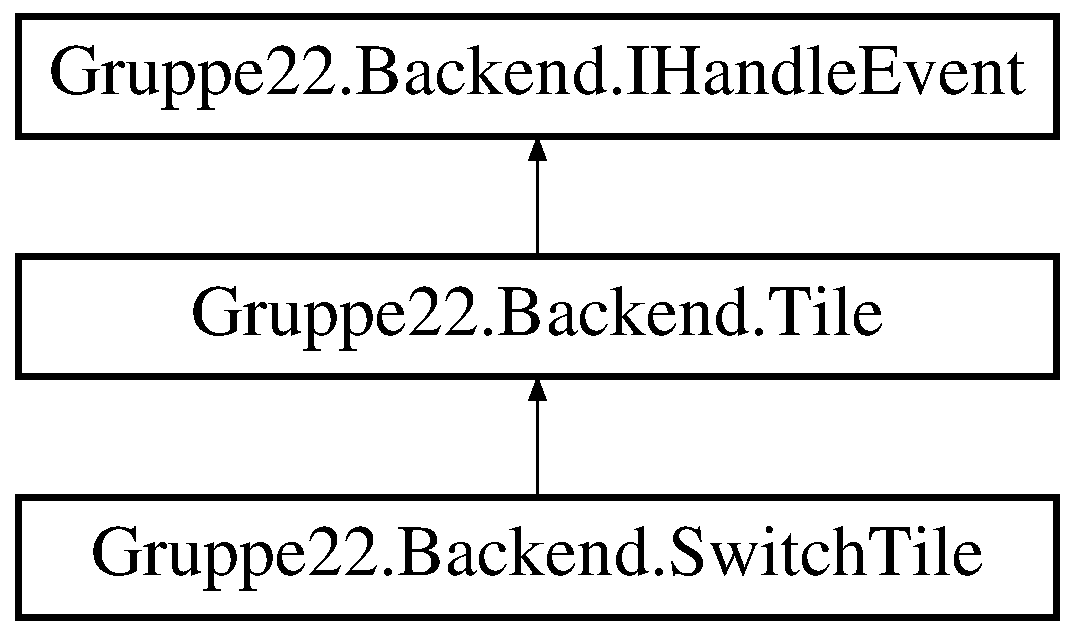
\includegraphics[height=3.000000cm]{class_gruppe22_1_1_backend_1_1_switch_tile}
\end{center}
\end{figure}
\subsection*{Öffentliche Methoden}
\begin{DoxyCompactItemize}
\item 
\hyperlink{class_gruppe22_1_1_backend_1_1_switch_tile_a661354802865cb1432b44c0b6864d95f}{Switch\-Tile} (object \hyperlink{class_gruppe22_1_1_backend_1_1_tile_abc12933c70eb3a2ebbb2fde9f45c2632}{parent})
\item 
override void \hyperlink{class_gruppe22_1_1_backend_1_1_switch_tile_aa50a0cf7dde944e73b9b2640042e78d2}{Save} (Xml\-Writer xmlw)
\begin{DoxyCompactList}\small\item\em Abstract method to save a tile in a X\-M\-L file \end{DoxyCompactList}\end{DoxyCompactItemize}
\subsection*{Propertys}
\begin{DoxyCompactItemize}
\item 
bool \hyperlink{class_gruppe22_1_1_backend_1_1_switch_tile_a7a0ef729ce23a17b4e1439407f618bfa}{active}\hspace{0.3cm}{\ttfamily  \mbox{[}get, set\mbox{]}}
\begin{DoxyCompactList}\small\item\em Whether the switch is active \end{DoxyCompactList}\item 
int \hyperlink{class_gruppe22_1_1_backend_1_1_switch_tile_aea9244b860d045796784dc1c00a90e13}{id}\hspace{0.3cm}{\ttfamily  \mbox{[}get, set\mbox{]}}
\begin{DoxyCompactList}\small\item\em Unique I\-D of switch (may be used as reference to door or trap) \end{DoxyCompactList}\item 
int \hyperlink{class_gruppe22_1_1_backend_1_1_switch_tile_ac060d5061b7ce694bd90fb7588aefdea}{order}\hspace{0.3cm}{\ttfamily  \mbox{[}get, set\mbox{]}}
\begin{DoxyCompactList}\small\item\em 0 based order in which switch status was changed \end{DoxyCompactList}\end{DoxyCompactItemize}
\subsection*{Weitere Geerbte Elemente}


\subsection{Beschreibung der Konstruktoren und Destruktoren}
\hypertarget{class_gruppe22_1_1_backend_1_1_switch_tile_a661354802865cb1432b44c0b6864d95f}{\index{Gruppe22\-::\-Backend\-::\-Switch\-Tile@{Gruppe22\-::\-Backend\-::\-Switch\-Tile}!Switch\-Tile@{Switch\-Tile}}
\index{Switch\-Tile@{Switch\-Tile}!Gruppe22::Backend::SwitchTile@{Gruppe22\-::\-Backend\-::\-Switch\-Tile}}
\subsubsection[{Switch\-Tile}]{\setlength{\rightskip}{0pt plus 5cm}Gruppe22.\-Backend.\-Switch\-Tile.\-Switch\-Tile (
\begin{DoxyParamCaption}
\item[{object}]{parent}
\end{DoxyParamCaption}
)}}\label{class_gruppe22_1_1_backend_1_1_switch_tile_a661354802865cb1432b44c0b6864d95f}


\subsection{Dokumentation der Elementfunktionen}
\hypertarget{class_gruppe22_1_1_backend_1_1_switch_tile_aa50a0cf7dde944e73b9b2640042e78d2}{\index{Gruppe22\-::\-Backend\-::\-Switch\-Tile@{Gruppe22\-::\-Backend\-::\-Switch\-Tile}!Save@{Save}}
\index{Save@{Save}!Gruppe22::Backend::SwitchTile@{Gruppe22\-::\-Backend\-::\-Switch\-Tile}}
\subsubsection[{Save}]{\setlength{\rightskip}{0pt plus 5cm}override void Gruppe22.\-Backend.\-Switch\-Tile.\-Save (
\begin{DoxyParamCaption}
\item[{Xml\-Writer}]{xmlw}
\end{DoxyParamCaption}
)\hspace{0.3cm}{\ttfamily [virtual]}}}\label{class_gruppe22_1_1_backend_1_1_switch_tile_aa50a0cf7dde944e73b9b2640042e78d2}


Abstract method to save a tile in a X\-M\-L file 


\begin{DoxyParams}{Parameter}
{\em xmlw} & the Xml\-Writer used for saving the file\\
\hline
\end{DoxyParams}


Erneute Implementation von \hyperlink{class_gruppe22_1_1_backend_1_1_tile_a109ab3e77ffca9d44c95a711af3491dc}{Gruppe22.\-Backend.\-Tile}.



\subsection{Dokumentation der Propertys}
\hypertarget{class_gruppe22_1_1_backend_1_1_switch_tile_a7a0ef729ce23a17b4e1439407f618bfa}{\index{Gruppe22\-::\-Backend\-::\-Switch\-Tile@{Gruppe22\-::\-Backend\-::\-Switch\-Tile}!active@{active}}
\index{active@{active}!Gruppe22::Backend::SwitchTile@{Gruppe22\-::\-Backend\-::\-Switch\-Tile}}
\subsubsection[{active}]{\setlength{\rightskip}{0pt plus 5cm}bool Gruppe22.\-Backend.\-Switch\-Tile.\-active\hspace{0.3cm}{\ttfamily [get]}, {\ttfamily [set]}}}\label{class_gruppe22_1_1_backend_1_1_switch_tile_a7a0ef729ce23a17b4e1439407f618bfa}


Whether the switch is active 

\hypertarget{class_gruppe22_1_1_backend_1_1_switch_tile_aea9244b860d045796784dc1c00a90e13}{\index{Gruppe22\-::\-Backend\-::\-Switch\-Tile@{Gruppe22\-::\-Backend\-::\-Switch\-Tile}!id@{id}}
\index{id@{id}!Gruppe22::Backend::SwitchTile@{Gruppe22\-::\-Backend\-::\-Switch\-Tile}}
\subsubsection[{id}]{\setlength{\rightskip}{0pt plus 5cm}int Gruppe22.\-Backend.\-Switch\-Tile.\-id\hspace{0.3cm}{\ttfamily [get]}, {\ttfamily [set]}}}\label{class_gruppe22_1_1_backend_1_1_switch_tile_aea9244b860d045796784dc1c00a90e13}


Unique I\-D of switch (may be used as reference to door or trap) 

\hypertarget{class_gruppe22_1_1_backend_1_1_switch_tile_ac060d5061b7ce694bd90fb7588aefdea}{\index{Gruppe22\-::\-Backend\-::\-Switch\-Tile@{Gruppe22\-::\-Backend\-::\-Switch\-Tile}!order@{order}}
\index{order@{order}!Gruppe22::Backend::SwitchTile@{Gruppe22\-::\-Backend\-::\-Switch\-Tile}}
\subsubsection[{order}]{\setlength{\rightskip}{0pt plus 5cm}int Gruppe22.\-Backend.\-Switch\-Tile.\-order\hspace{0.3cm}{\ttfamily [get]}, {\ttfamily [set]}}}\label{class_gruppe22_1_1_backend_1_1_switch_tile_ac060d5061b7ce694bd90fb7588aefdea}


0 based order in which switch status was changed 



Die Dokumentation für diese Klasse wurde erzeugt aufgrund der Datei\-:\begin{DoxyCompactItemize}
\item 
C\-:/\-Users/beursken/\-Documents/\-Git\-Hub/gruppe22/\-Gruppe22/\-Gruppe22/\-Backend/\-Map/\hyperlink{_switch_tile_8cs}{Switch\-Tile.\-cs}\end{DoxyCompactItemize}

\hypertarget{class_gruppe22_1_1_backend_1_1_target_tile}{\section{Gruppe22.\-Backend.\-Target\-Tile Klassenreferenz}
\label{class_gruppe22_1_1_backend_1_1_target_tile}\index{Gruppe22.\-Backend.\-Target\-Tile@{Gruppe22.\-Backend.\-Target\-Tile}}
}
Klassendiagramm für Gruppe22.\-Backend.\-Target\-Tile\-:\begin{figure}[H]
\begin{center}
\leavevmode
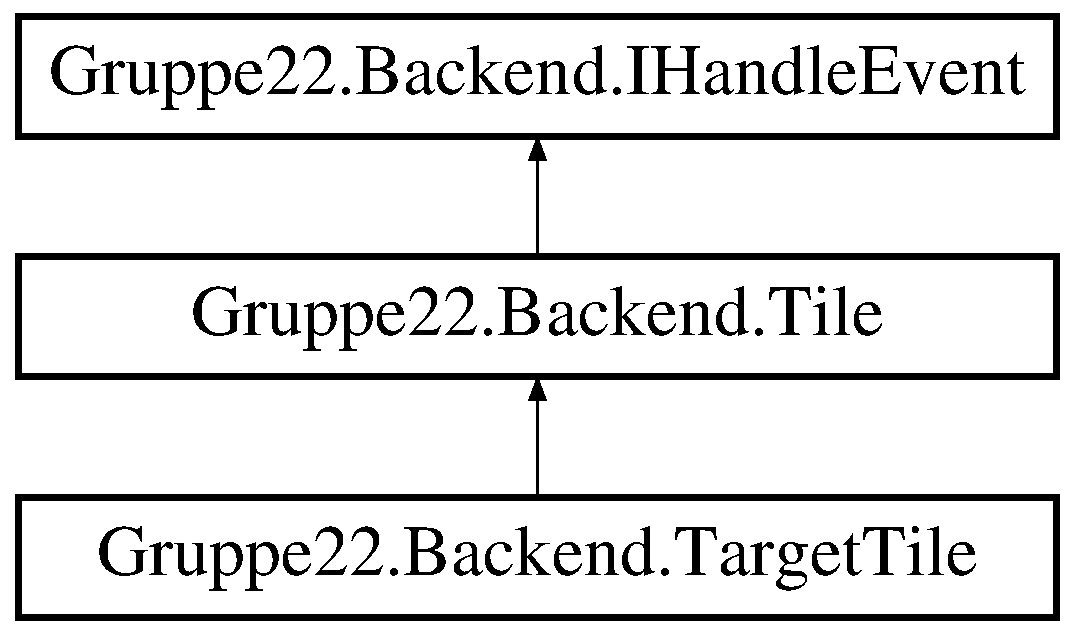
\includegraphics[height=3.000000cm]{class_gruppe22_1_1_backend_1_1_target_tile}
\end{center}
\end{figure}
\subsection*{Öffentliche Methoden}
\begin{DoxyCompactItemize}
\item 
\hyperlink{class_gruppe22_1_1_backend_1_1_target_tile_a1149b7f5f68a087f1cb11ad4e2851a60}{Target\-Tile} (object \hyperlink{class_gruppe22_1_1_backend_1_1_tile_abc12933c70eb3a2ebbb2fde9f45c2632}{parent})
\item 
override void \hyperlink{class_gruppe22_1_1_backend_1_1_target_tile_a3bb3f1712e44d11503f5da8226cba9f6}{Save} (Xml\-Writer xmlw)
\begin{DoxyCompactList}\small\item\em Abstract method to save a tile in a X\-M\-L file \end{DoxyCompactList}\end{DoxyCompactItemize}
\subsection*{Weitere Geerbte Elemente}


\subsection{Beschreibung der Konstruktoren und Destruktoren}
\hypertarget{class_gruppe22_1_1_backend_1_1_target_tile_a1149b7f5f68a087f1cb11ad4e2851a60}{\index{Gruppe22\-::\-Backend\-::\-Target\-Tile@{Gruppe22\-::\-Backend\-::\-Target\-Tile}!Target\-Tile@{Target\-Tile}}
\index{Target\-Tile@{Target\-Tile}!Gruppe22::Backend::TargetTile@{Gruppe22\-::\-Backend\-::\-Target\-Tile}}
\subsubsection[{Target\-Tile}]{\setlength{\rightskip}{0pt plus 5cm}Gruppe22.\-Backend.\-Target\-Tile.\-Target\-Tile (
\begin{DoxyParamCaption}
\item[{object}]{parent}
\end{DoxyParamCaption}
)}}\label{class_gruppe22_1_1_backend_1_1_target_tile_a1149b7f5f68a087f1cb11ad4e2851a60}


\subsection{Dokumentation der Elementfunktionen}
\hypertarget{class_gruppe22_1_1_backend_1_1_target_tile_a3bb3f1712e44d11503f5da8226cba9f6}{\index{Gruppe22\-::\-Backend\-::\-Target\-Tile@{Gruppe22\-::\-Backend\-::\-Target\-Tile}!Save@{Save}}
\index{Save@{Save}!Gruppe22::Backend::TargetTile@{Gruppe22\-::\-Backend\-::\-Target\-Tile}}
\subsubsection[{Save}]{\setlength{\rightskip}{0pt plus 5cm}override void Gruppe22.\-Backend.\-Target\-Tile.\-Save (
\begin{DoxyParamCaption}
\item[{Xml\-Writer}]{xmlw}
\end{DoxyParamCaption}
)\hspace{0.3cm}{\ttfamily [virtual]}}}\label{class_gruppe22_1_1_backend_1_1_target_tile_a3bb3f1712e44d11503f5da8226cba9f6}


Abstract method to save a tile in a X\-M\-L file 


\begin{DoxyParams}{Parameter}
{\em xmlw} & the Xml\-Writer used for saving the file\\
\hline
\end{DoxyParams}


Erneute Implementation von \hyperlink{class_gruppe22_1_1_backend_1_1_tile_a109ab3e77ffca9d44c95a711af3491dc}{Gruppe22.\-Backend.\-Tile}.



Die Dokumentation für diese Klasse wurde erzeugt aufgrund der Datei\-:\begin{DoxyCompactItemize}
\item 
C\-:/\-Users/beursken/\-Documents/\-Git\-Hub/gruppe22/\-Gruppe22/\-Gruppe22/\-Backend/\-Map/\hyperlink{_target_tile_8cs}{Target\-Tile.\-cs}\end{DoxyCompactItemize}

\hypertarget{class_gruppe22_1_1_backend_1_1_teleport_tile}{\section{Gruppe22.\-Backend.\-Teleport\-Tile Klassenreferenz}
\label{class_gruppe22_1_1_backend_1_1_teleport_tile}\index{Gruppe22.\-Backend.\-Teleport\-Tile@{Gruppe22.\-Backend.\-Teleport\-Tile}}
}
Klassendiagramm für Gruppe22.\-Backend.\-Teleport\-Tile\-:\begin{figure}[H]
\begin{center}
\leavevmode
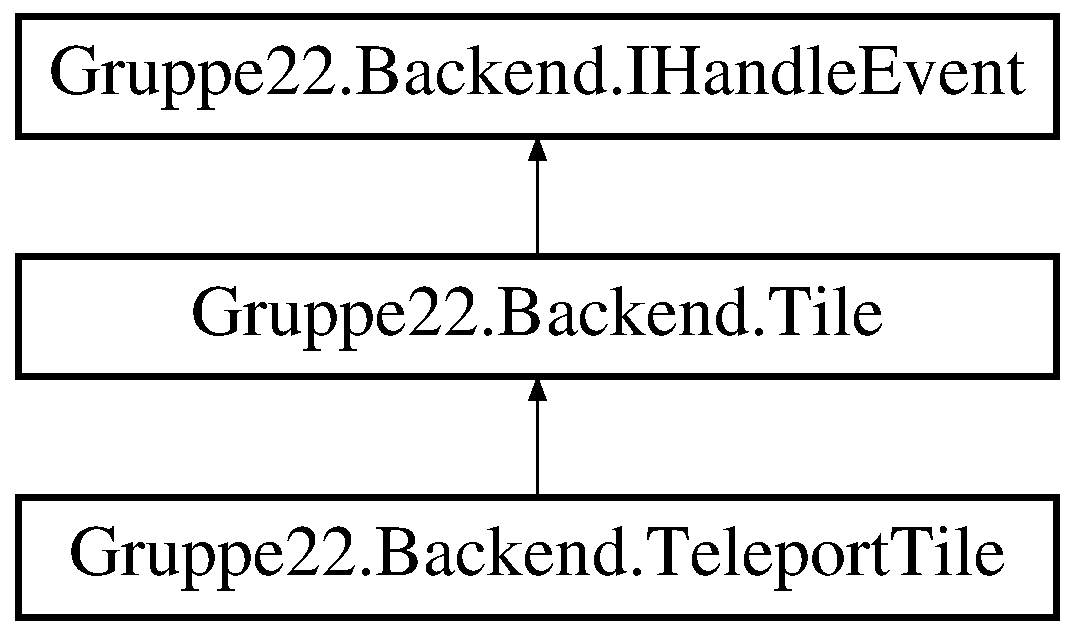
\includegraphics[height=3.000000cm]{class_gruppe22_1_1_backend_1_1_teleport_tile}
\end{center}
\end{figure}
\subsection*{Öffentliche Methoden}
\begin{DoxyCompactItemize}
\item 
\hyperlink{class_gruppe22_1_1_backend_1_1_teleport_tile_a075d6c22572655624590fd57147e66d3}{Teleport\-Tile} (object \hyperlink{class_gruppe22_1_1_backend_1_1_tile_abc12933c70eb3a2ebbb2fde9f45c2632}{parent}, string next\-Xml, \hyperlink{class_gruppe22_1_1_backend_1_1_coords}{Backend.\-Coords} pos, bool is\-Teleport=false, bool is\-Hidden=false, bool is\-Enabled=true, bool is\-Up=false)
\item 
override void \hyperlink{class_gruppe22_1_1_backend_1_1_teleport_tile_a15a8abf308bcb1577fdea70a4959bf79}{Save} (Xml\-Writer xmlw)
\begin{DoxyCompactList}\small\item\em Abstract method to save a tile in a X\-M\-L file \end{DoxyCompactList}\end{DoxyCompactItemize}
\subsection*{Propertys}
\begin{DoxyCompactItemize}
\item 
String \hyperlink{class_gruppe22_1_1_backend_1_1_teleport_tile_a133def222075e29e9434e8ffb4e4bf1a}{next\-Room}\hspace{0.3cm}{\ttfamily  \mbox{[}get, set\mbox{]}}
\item 
\hyperlink{class_gruppe22_1_1_backend_1_1_coords}{Backend.\-Coords} \hyperlink{class_gruppe22_1_1_backend_1_1_teleport_tile_ab83627306a280afbfadb8441b6df0485}{next\-Player\-Pos}\hspace{0.3cm}{\ttfamily  \mbox{[}get\mbox{]}}
\item 
bool \hyperlink{class_gruppe22_1_1_backend_1_1_teleport_tile_abee7ec642fbd77e0d6b16105aa42b589}{hidden}\hspace{0.3cm}{\ttfamily  \mbox{[}get, set\mbox{]}}
\item 
bool \hyperlink{class_gruppe22_1_1_backend_1_1_teleport_tile_ac83bb7b79fd78d4c91114629c5306cc8}{enabled}\hspace{0.3cm}{\ttfamily  \mbox{[}get, set\mbox{]}}
\item 
bool \hyperlink{class_gruppe22_1_1_backend_1_1_teleport_tile_aad5853c299ee66afac5565812cabdf52}{teleport}\hspace{0.3cm}{\ttfamily  \mbox{[}get, set\mbox{]}}
\item 
bool \hyperlink{class_gruppe22_1_1_backend_1_1_teleport_tile_a0730a9a54b6e01a66e2db7db4e33de49}{down}\hspace{0.3cm}{\ttfamily  \mbox{[}get, set\mbox{]}}
\end{DoxyCompactItemize}
\subsection*{Weitere Geerbte Elemente}


\subsection{Beschreibung der Konstruktoren und Destruktoren}
\hypertarget{class_gruppe22_1_1_backend_1_1_teleport_tile_a075d6c22572655624590fd57147e66d3}{\index{Gruppe22\-::\-Backend\-::\-Teleport\-Tile@{Gruppe22\-::\-Backend\-::\-Teleport\-Tile}!Teleport\-Tile@{Teleport\-Tile}}
\index{Teleport\-Tile@{Teleport\-Tile}!Gruppe22::Backend::TeleportTile@{Gruppe22\-::\-Backend\-::\-Teleport\-Tile}}
\subsubsection[{Teleport\-Tile}]{\setlength{\rightskip}{0pt plus 5cm}Gruppe22.\-Backend.\-Teleport\-Tile.\-Teleport\-Tile (
\begin{DoxyParamCaption}
\item[{object}]{parent, }
\item[{string}]{next\-Xml, }
\item[{{\bf Backend.\-Coords}}]{pos, }
\item[{bool}]{is\-Teleport = {\ttfamily false}, }
\item[{bool}]{is\-Hidden = {\ttfamily false}, }
\item[{bool}]{is\-Enabled = {\ttfamily true}, }
\item[{bool}]{is\-Up = {\ttfamily false}}
\end{DoxyParamCaption}
)}}\label{class_gruppe22_1_1_backend_1_1_teleport_tile_a075d6c22572655624590fd57147e66d3}


\subsection{Dokumentation der Elementfunktionen}
\hypertarget{class_gruppe22_1_1_backend_1_1_teleport_tile_a15a8abf308bcb1577fdea70a4959bf79}{\index{Gruppe22\-::\-Backend\-::\-Teleport\-Tile@{Gruppe22\-::\-Backend\-::\-Teleport\-Tile}!Save@{Save}}
\index{Save@{Save}!Gruppe22::Backend::TeleportTile@{Gruppe22\-::\-Backend\-::\-Teleport\-Tile}}
\subsubsection[{Save}]{\setlength{\rightskip}{0pt plus 5cm}override void Gruppe22.\-Backend.\-Teleport\-Tile.\-Save (
\begin{DoxyParamCaption}
\item[{Xml\-Writer}]{xmlw}
\end{DoxyParamCaption}
)\hspace{0.3cm}{\ttfamily [virtual]}}}\label{class_gruppe22_1_1_backend_1_1_teleport_tile_a15a8abf308bcb1577fdea70a4959bf79}


Abstract method to save a tile in a X\-M\-L file 


\begin{DoxyParams}{Parameter}
{\em xmlw} & the Xml\-Writer used for saving the file\\
\hline
\end{DoxyParams}


Erneute Implementation von \hyperlink{class_gruppe22_1_1_backend_1_1_tile_a109ab3e77ffca9d44c95a711af3491dc}{Gruppe22.\-Backend.\-Tile}.



\subsection{Dokumentation der Propertys}
\hypertarget{class_gruppe22_1_1_backend_1_1_teleport_tile_a0730a9a54b6e01a66e2db7db4e33de49}{\index{Gruppe22\-::\-Backend\-::\-Teleport\-Tile@{Gruppe22\-::\-Backend\-::\-Teleport\-Tile}!down@{down}}
\index{down@{down}!Gruppe22::Backend::TeleportTile@{Gruppe22\-::\-Backend\-::\-Teleport\-Tile}}
\subsubsection[{down}]{\setlength{\rightskip}{0pt plus 5cm}bool Gruppe22.\-Backend.\-Teleport\-Tile.\-down\hspace{0.3cm}{\ttfamily [get]}, {\ttfamily [set]}}}\label{class_gruppe22_1_1_backend_1_1_teleport_tile_a0730a9a54b6e01a66e2db7db4e33de49}
\hypertarget{class_gruppe22_1_1_backend_1_1_teleport_tile_ac83bb7b79fd78d4c91114629c5306cc8}{\index{Gruppe22\-::\-Backend\-::\-Teleport\-Tile@{Gruppe22\-::\-Backend\-::\-Teleport\-Tile}!enabled@{enabled}}
\index{enabled@{enabled}!Gruppe22::Backend::TeleportTile@{Gruppe22\-::\-Backend\-::\-Teleport\-Tile}}
\subsubsection[{enabled}]{\setlength{\rightskip}{0pt plus 5cm}bool Gruppe22.\-Backend.\-Teleport\-Tile.\-enabled\hspace{0.3cm}{\ttfamily [get]}, {\ttfamily [set]}}}\label{class_gruppe22_1_1_backend_1_1_teleport_tile_ac83bb7b79fd78d4c91114629c5306cc8}
\hypertarget{class_gruppe22_1_1_backend_1_1_teleport_tile_abee7ec642fbd77e0d6b16105aa42b589}{\index{Gruppe22\-::\-Backend\-::\-Teleport\-Tile@{Gruppe22\-::\-Backend\-::\-Teleport\-Tile}!hidden@{hidden}}
\index{hidden@{hidden}!Gruppe22::Backend::TeleportTile@{Gruppe22\-::\-Backend\-::\-Teleport\-Tile}}
\subsubsection[{hidden}]{\setlength{\rightskip}{0pt plus 5cm}bool Gruppe22.\-Backend.\-Teleport\-Tile.\-hidden\hspace{0.3cm}{\ttfamily [get]}, {\ttfamily [set]}}}\label{class_gruppe22_1_1_backend_1_1_teleport_tile_abee7ec642fbd77e0d6b16105aa42b589}
\hypertarget{class_gruppe22_1_1_backend_1_1_teleport_tile_ab83627306a280afbfadb8441b6df0485}{\index{Gruppe22\-::\-Backend\-::\-Teleport\-Tile@{Gruppe22\-::\-Backend\-::\-Teleport\-Tile}!next\-Player\-Pos@{next\-Player\-Pos}}
\index{next\-Player\-Pos@{next\-Player\-Pos}!Gruppe22::Backend::TeleportTile@{Gruppe22\-::\-Backend\-::\-Teleport\-Tile}}
\subsubsection[{next\-Player\-Pos}]{\setlength{\rightskip}{0pt plus 5cm}{\bf Backend.\-Coords} Gruppe22.\-Backend.\-Teleport\-Tile.\-next\-Player\-Pos\hspace{0.3cm}{\ttfamily [get]}}}\label{class_gruppe22_1_1_backend_1_1_teleport_tile_ab83627306a280afbfadb8441b6df0485}
\hypertarget{class_gruppe22_1_1_backend_1_1_teleport_tile_a133def222075e29e9434e8ffb4e4bf1a}{\index{Gruppe22\-::\-Backend\-::\-Teleport\-Tile@{Gruppe22\-::\-Backend\-::\-Teleport\-Tile}!next\-Room@{next\-Room}}
\index{next\-Room@{next\-Room}!Gruppe22::Backend::TeleportTile@{Gruppe22\-::\-Backend\-::\-Teleport\-Tile}}
\subsubsection[{next\-Room}]{\setlength{\rightskip}{0pt plus 5cm}String Gruppe22.\-Backend.\-Teleport\-Tile.\-next\-Room\hspace{0.3cm}{\ttfamily [get]}, {\ttfamily [set]}}}\label{class_gruppe22_1_1_backend_1_1_teleport_tile_a133def222075e29e9434e8ffb4e4bf1a}
\hypertarget{class_gruppe22_1_1_backend_1_1_teleport_tile_aad5853c299ee66afac5565812cabdf52}{\index{Gruppe22\-::\-Backend\-::\-Teleport\-Tile@{Gruppe22\-::\-Backend\-::\-Teleport\-Tile}!teleport@{teleport}}
\index{teleport@{teleport}!Gruppe22::Backend::TeleportTile@{Gruppe22\-::\-Backend\-::\-Teleport\-Tile}}
\subsubsection[{teleport}]{\setlength{\rightskip}{0pt plus 5cm}bool Gruppe22.\-Backend.\-Teleport\-Tile.\-teleport\hspace{0.3cm}{\ttfamily [get]}, {\ttfamily [set]}}}\label{class_gruppe22_1_1_backend_1_1_teleport_tile_aad5853c299ee66afac5565812cabdf52}


Die Dokumentation für diese Klasse wurde erzeugt aufgrund der Datei\-:\begin{DoxyCompactItemize}
\item 
C\-:/\-Users/beursken/\-Documents/\-Git\-Hub/gruppe22/\-Gruppe22/\-Gruppe22/\-Backend/\-Map/\hyperlink{_teleport_tile_8cs}{Teleport\-Tile.\-cs}\end{DoxyCompactItemize}

\hypertarget{class_gruppe22_1_1_client_1_1_text_input}{\section{Gruppe22.\-Client.\-Text\-Input Klassenreferenz}
\label{class_gruppe22_1_1_client_1_1_text_input}\index{Gruppe22.\-Client.\-Text\-Input@{Gruppe22.\-Client.\-Text\-Input}}
}
Klassendiagramm für Gruppe22.\-Client.\-Text\-Input\-:\begin{figure}[H]
\begin{center}
\leavevmode
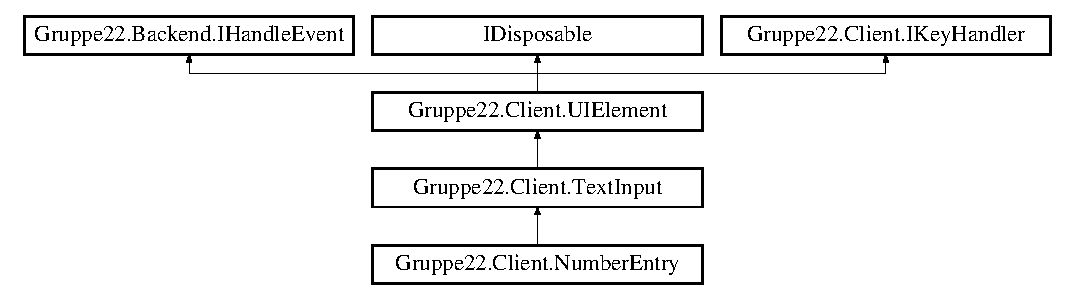
\includegraphics[height=3.589744cm]{class_gruppe22_1_1_client_1_1_text_input}
\end{center}
\end{figure}
\subsection*{Öffentliche Methoden}
\begin{DoxyCompactItemize}
\item 
override bool \hyperlink{class_gruppe22_1_1_client_1_1_text_input_aa1122f9fe72ced8d5673e20e279beff4}{On\-Key\-Down} (Microsoft.\-Xna.\-Framework.\-Input.\-Keys k)
\item 
override void \hyperlink{class_gruppe22_1_1_client_1_1_text_input_ac687504d29f26d40baefd69fb9537d92}{Handle\-Event} (bool Down\-Stream, \hyperlink{namespace_gruppe22_1_1_backend_ab56df91bb0bdafa1ea978e552209ce73}{Backend.\-Events} event\-I\-D, params object\mbox{[}$\,$\mbox{]} data)
\item 
override void \hyperlink{class_gruppe22_1_1_client_1_1_text_input_a39d2aeb6a1bf78d643688d79d009c3ae}{Draw} (Game\-Time game\-Time)
\item 
override void \hyperlink{class_gruppe22_1_1_client_1_1_text_input_aeb12ff2ec36009368ef79b71eb39fa73}{Update} (Game\-Time game\-Time)
\item 
\hyperlink{class_gruppe22_1_1_client_1_1_text_input_aec93a57386f2255d76e0134241bcd1be}{Text\-Input} (\hyperlink{interface_gruppe22_1_1_backend_1_1_i_handle_event}{Backend.\-I\-Handle\-Event} parent, Sprite\-Batch sprite\-Batch, Content\-Manager content, Rectangle display\-Rect, string label, string \hyperlink{class_gruppe22_1_1_client_1_1_text_input_a795e9f3cdc6b089dc1cc864907b33f44}{text}, string tool\-Tip, int input\-Width, bool \hyperlink{class_gruppe22_1_1_client_1_1_text_input_ae512171e8f7caead8c28eb9327ccbf40}{can\-Edit})
\end{DoxyCompactItemize}
\subsection*{Geschützte Methoden}
\begin{DoxyCompactItemize}
\item 
void \hyperlink{class_gruppe22_1_1_client_1_1_text_input_a607de727ce5b80faa8134c448ca4da62}{\-\_\-\-Display\-Tool\-Tip} ()
\begin{DoxyCompactList}\small\item\em Append a new line of text to the status box; word wrap if necessary \end{DoxyCompactList}\end{DoxyCompactItemize}
\subsection*{Geschützte Attribute}
\begin{DoxyCompactItemize}
\item 
string \hyperlink{class_gruppe22_1_1_client_1_1_text_input_a725d60af4b5f21d1240f3aefb98a849e}{\-\_\-label} = \char`\"{}\char`\"{}
\item 
string \hyperlink{class_gruppe22_1_1_client_1_1_text_input_a829d2cea87b902b6a62cc3ac904e0592}{\-\_\-text} = \char`\"{}\char`\"{}
\item 
string \hyperlink{class_gruppe22_1_1_client_1_1_text_input_a53174a0caffcd22e7327967ceb3bc9a5}{\-\_\-tooltip} = \char`\"{}\char`\"{}
\item 
Sprite\-Font \hyperlink{class_gruppe22_1_1_client_1_1_text_input_afaa8c705ebedf4acf422f4de1b1f6f71}{\-\_\-font} = null
\item 
Texture2\-D \hyperlink{class_gruppe22_1_1_client_1_1_text_input_aad2ed3307a1e3dd8684a0aba48bfe55d}{\-\_\-background} = null
\item 
int \hyperlink{class_gruppe22_1_1_client_1_1_text_input_a9c383c0270cf48278e25aeb04afc54c2}{\-\_\-text\-Width} = 0
\item 
bool \hyperlink{class_gruppe22_1_1_client_1_1_text_input_a97938831e8ee83ad77e160ea51428505}{\-\_\-can\-Edit} = false
\end{DoxyCompactItemize}
\subsection*{Propertys}
\begin{DoxyCompactItemize}
\item 
string \hyperlink{class_gruppe22_1_1_client_1_1_text_input_a795e9f3cdc6b089dc1cc864907b33f44}{text}\hspace{0.3cm}{\ttfamily  \mbox{[}get, set\mbox{]}}
\item 
override bool \hyperlink{class_gruppe22_1_1_client_1_1_text_input_ac50c924f3a99583da29fe82ff09c876e}{can\-Focus}\hspace{0.3cm}{\ttfamily  \mbox{[}get\mbox{]}}
\item 
bool \hyperlink{class_gruppe22_1_1_client_1_1_text_input_ae512171e8f7caead8c28eb9327ccbf40}{can\-Edit}\hspace{0.3cm}{\ttfamily  \mbox{[}get, set\mbox{]}}
\end{DoxyCompactItemize}


\subsection{Beschreibung der Konstruktoren und Destruktoren}
\hypertarget{class_gruppe22_1_1_client_1_1_text_input_aec93a57386f2255d76e0134241bcd1be}{\index{Gruppe22\-::\-Client\-::\-Text\-Input@{Gruppe22\-::\-Client\-::\-Text\-Input}!Text\-Input@{Text\-Input}}
\index{Text\-Input@{Text\-Input}!Gruppe22::Client::TextInput@{Gruppe22\-::\-Client\-::\-Text\-Input}}
\subsubsection[{Text\-Input}]{\setlength{\rightskip}{0pt plus 5cm}Gruppe22.\-Client.\-Text\-Input.\-Text\-Input (
\begin{DoxyParamCaption}
\item[{{\bf Backend.\-I\-Handle\-Event}}]{parent, }
\item[{Sprite\-Batch}]{sprite\-Batch, }
\item[{Content\-Manager}]{content, }
\item[{Rectangle}]{display\-Rect, }
\item[{string}]{label, }
\item[{string}]{text, }
\item[{string}]{tool\-Tip, }
\item[{int}]{input\-Width, }
\item[{bool}]{can\-Edit}
\end{DoxyParamCaption}
)}}\label{class_gruppe22_1_1_client_1_1_text_input_aec93a57386f2255d76e0134241bcd1be}





\begin{DoxyParams}{Parameter}
{\em parent} & \\
\hline
{\em sprite\-Batch} & \\
\hline
{\em content} & \\
\hline
{\em display\-Rect} & \\
\hline
\end{DoxyParams}


\subsection{Dokumentation der Elementfunktionen}
\hypertarget{class_gruppe22_1_1_client_1_1_text_input_a607de727ce5b80faa8134c448ca4da62}{\index{Gruppe22\-::\-Client\-::\-Text\-Input@{Gruppe22\-::\-Client\-::\-Text\-Input}!\-\_\-\-Display\-Tool\-Tip@{\-\_\-\-Display\-Tool\-Tip}}
\index{\-\_\-\-Display\-Tool\-Tip@{\-\_\-\-Display\-Tool\-Tip}!Gruppe22::Client::TextInput@{Gruppe22\-::\-Client\-::\-Text\-Input}}
\subsubsection[{\-\_\-\-Display\-Tool\-Tip}]{\setlength{\rightskip}{0pt plus 5cm}void Gruppe22.\-Client.\-Text\-Input.\-\_\-\-Display\-Tool\-Tip (
\begin{DoxyParamCaption}
{}
\end{DoxyParamCaption}
)\hspace{0.3cm}{\ttfamily [protected]}}}\label{class_gruppe22_1_1_client_1_1_text_input_a607de727ce5b80faa8134c448ca4da62}


Append a new line of text to the status box; word wrap if necessary 


\begin{DoxyParams}{Parameter}
{\em text} & \\
\hline
\end{DoxyParams}
\hypertarget{class_gruppe22_1_1_client_1_1_text_input_a39d2aeb6a1bf78d643688d79d009c3ae}{\index{Gruppe22\-::\-Client\-::\-Text\-Input@{Gruppe22\-::\-Client\-::\-Text\-Input}!Draw@{Draw}}
\index{Draw@{Draw}!Gruppe22::Client::TextInput@{Gruppe22\-::\-Client\-::\-Text\-Input}}
\subsubsection[{Draw}]{\setlength{\rightskip}{0pt plus 5cm}override void Gruppe22.\-Client.\-Text\-Input.\-Draw (
\begin{DoxyParamCaption}
\item[{Game\-Time}]{game\-Time}
\end{DoxyParamCaption}
)\hspace{0.3cm}{\ttfamily [virtual]}}}\label{class_gruppe22_1_1_client_1_1_text_input_a39d2aeb6a1bf78d643688d79d009c3ae}





\begin{DoxyParams}{Parameter}
{\em game\-Time} & \\
\hline
\end{DoxyParams}


Erneute Implementation von \hyperlink{class_gruppe22_1_1_client_1_1_u_i_element_ae68afcbd1db3540052d6b399022e56e7}{Gruppe22.\-Client.\-U\-I\-Element}.

\hypertarget{class_gruppe22_1_1_client_1_1_text_input_ac687504d29f26d40baefd69fb9537d92}{\index{Gruppe22\-::\-Client\-::\-Text\-Input@{Gruppe22\-::\-Client\-::\-Text\-Input}!Handle\-Event@{Handle\-Event}}
\index{Handle\-Event@{Handle\-Event}!Gruppe22::Client::TextInput@{Gruppe22\-::\-Client\-::\-Text\-Input}}
\subsubsection[{Handle\-Event}]{\setlength{\rightskip}{0pt plus 5cm}override void Gruppe22.\-Client.\-Text\-Input.\-Handle\-Event (
\begin{DoxyParamCaption}
\item[{bool}]{Down\-Stream, }
\item[{{\bf Backend.\-Events}}]{event\-I\-D, }
\item[{params object\mbox{[}$\,$\mbox{]}}]{data}
\end{DoxyParamCaption}
)\hspace{0.3cm}{\ttfamily [virtual]}}}\label{class_gruppe22_1_1_client_1_1_text_input_ac687504d29f26d40baefd69fb9537d92}


Erneute Implementation von \hyperlink{class_gruppe22_1_1_client_1_1_u_i_element_ad06a1ce6c1705a1c7aa91756f368a517}{Gruppe22.\-Client.\-U\-I\-Element}.

\hypertarget{class_gruppe22_1_1_client_1_1_text_input_aa1122f9fe72ced8d5673e20e279beff4}{\index{Gruppe22\-::\-Client\-::\-Text\-Input@{Gruppe22\-::\-Client\-::\-Text\-Input}!On\-Key\-Down@{On\-Key\-Down}}
\index{On\-Key\-Down@{On\-Key\-Down}!Gruppe22::Client::TextInput@{Gruppe22\-::\-Client\-::\-Text\-Input}}
\subsubsection[{On\-Key\-Down}]{\setlength{\rightskip}{0pt plus 5cm}override bool Gruppe22.\-Client.\-Text\-Input.\-On\-Key\-Down (
\begin{DoxyParamCaption}
\item[{Microsoft.\-Xna.\-Framework.\-Input.\-Keys}]{k}
\end{DoxyParamCaption}
)}}\label{class_gruppe22_1_1_client_1_1_text_input_aa1122f9fe72ced8d5673e20e279beff4}
\hypertarget{class_gruppe22_1_1_client_1_1_text_input_aeb12ff2ec36009368ef79b71eb39fa73}{\index{Gruppe22\-::\-Client\-::\-Text\-Input@{Gruppe22\-::\-Client\-::\-Text\-Input}!Update@{Update}}
\index{Update@{Update}!Gruppe22::Client::TextInput@{Gruppe22\-::\-Client\-::\-Text\-Input}}
\subsubsection[{Update}]{\setlength{\rightskip}{0pt plus 5cm}override void Gruppe22.\-Client.\-Text\-Input.\-Update (
\begin{DoxyParamCaption}
\item[{Game\-Time}]{game\-Time}
\end{DoxyParamCaption}
)\hspace{0.3cm}{\ttfamily [virtual]}}}\label{class_gruppe22_1_1_client_1_1_text_input_aeb12ff2ec36009368ef79b71eb39fa73}





\begin{DoxyParams}{Parameter}
{\em game\-Time} & \\
\hline
\end{DoxyParams}


Erneute Implementation von \hyperlink{class_gruppe22_1_1_client_1_1_u_i_element_a456bc763b6ed6ab441bb0ae96b6f4f8b}{Gruppe22.\-Client.\-U\-I\-Element}.



\subsection{Dokumentation der Datenelemente}
\hypertarget{class_gruppe22_1_1_client_1_1_text_input_aad2ed3307a1e3dd8684a0aba48bfe55d}{\index{Gruppe22\-::\-Client\-::\-Text\-Input@{Gruppe22\-::\-Client\-::\-Text\-Input}!\-\_\-background@{\-\_\-background}}
\index{\-\_\-background@{\-\_\-background}!Gruppe22::Client::TextInput@{Gruppe22\-::\-Client\-::\-Text\-Input}}
\subsubsection[{\-\_\-background}]{\setlength{\rightskip}{0pt plus 5cm}Texture2\-D Gruppe22.\-Client.\-Text\-Input.\-\_\-background = null\hspace{0.3cm}{\ttfamily [protected]}}}\label{class_gruppe22_1_1_client_1_1_text_input_aad2ed3307a1e3dd8684a0aba48bfe55d}
\hypertarget{class_gruppe22_1_1_client_1_1_text_input_a97938831e8ee83ad77e160ea51428505}{\index{Gruppe22\-::\-Client\-::\-Text\-Input@{Gruppe22\-::\-Client\-::\-Text\-Input}!\-\_\-can\-Edit@{\-\_\-can\-Edit}}
\index{\-\_\-can\-Edit@{\-\_\-can\-Edit}!Gruppe22::Client::TextInput@{Gruppe22\-::\-Client\-::\-Text\-Input}}
\subsubsection[{\-\_\-can\-Edit}]{\setlength{\rightskip}{0pt plus 5cm}bool Gruppe22.\-Client.\-Text\-Input.\-\_\-can\-Edit = false\hspace{0.3cm}{\ttfamily [protected]}}}\label{class_gruppe22_1_1_client_1_1_text_input_a97938831e8ee83ad77e160ea51428505}
\hypertarget{class_gruppe22_1_1_client_1_1_text_input_afaa8c705ebedf4acf422f4de1b1f6f71}{\index{Gruppe22\-::\-Client\-::\-Text\-Input@{Gruppe22\-::\-Client\-::\-Text\-Input}!\-\_\-font@{\-\_\-font}}
\index{\-\_\-font@{\-\_\-font}!Gruppe22::Client::TextInput@{Gruppe22\-::\-Client\-::\-Text\-Input}}
\subsubsection[{\-\_\-font}]{\setlength{\rightskip}{0pt plus 5cm}Sprite\-Font Gruppe22.\-Client.\-Text\-Input.\-\_\-font = null\hspace{0.3cm}{\ttfamily [protected]}}}\label{class_gruppe22_1_1_client_1_1_text_input_afaa8c705ebedf4acf422f4de1b1f6f71}
\hypertarget{class_gruppe22_1_1_client_1_1_text_input_a725d60af4b5f21d1240f3aefb98a849e}{\index{Gruppe22\-::\-Client\-::\-Text\-Input@{Gruppe22\-::\-Client\-::\-Text\-Input}!\-\_\-label@{\-\_\-label}}
\index{\-\_\-label@{\-\_\-label}!Gruppe22::Client::TextInput@{Gruppe22\-::\-Client\-::\-Text\-Input}}
\subsubsection[{\-\_\-label}]{\setlength{\rightskip}{0pt plus 5cm}string Gruppe22.\-Client.\-Text\-Input.\-\_\-label = \char`\"{}\char`\"{}\hspace{0.3cm}{\ttfamily [protected]}}}\label{class_gruppe22_1_1_client_1_1_text_input_a725d60af4b5f21d1240f3aefb98a849e}
\hypertarget{class_gruppe22_1_1_client_1_1_text_input_a829d2cea87b902b6a62cc3ac904e0592}{\index{Gruppe22\-::\-Client\-::\-Text\-Input@{Gruppe22\-::\-Client\-::\-Text\-Input}!\-\_\-text@{\-\_\-text}}
\index{\-\_\-text@{\-\_\-text}!Gruppe22::Client::TextInput@{Gruppe22\-::\-Client\-::\-Text\-Input}}
\subsubsection[{\-\_\-text}]{\setlength{\rightskip}{0pt plus 5cm}string Gruppe22.\-Client.\-Text\-Input.\-\_\-text = \char`\"{}\char`\"{}\hspace{0.3cm}{\ttfamily [protected]}}}\label{class_gruppe22_1_1_client_1_1_text_input_a829d2cea87b902b6a62cc3ac904e0592}
\hypertarget{class_gruppe22_1_1_client_1_1_text_input_a9c383c0270cf48278e25aeb04afc54c2}{\index{Gruppe22\-::\-Client\-::\-Text\-Input@{Gruppe22\-::\-Client\-::\-Text\-Input}!\-\_\-text\-Width@{\-\_\-text\-Width}}
\index{\-\_\-text\-Width@{\-\_\-text\-Width}!Gruppe22::Client::TextInput@{Gruppe22\-::\-Client\-::\-Text\-Input}}
\subsubsection[{\-\_\-text\-Width}]{\setlength{\rightskip}{0pt plus 5cm}int Gruppe22.\-Client.\-Text\-Input.\-\_\-text\-Width = 0\hspace{0.3cm}{\ttfamily [protected]}}}\label{class_gruppe22_1_1_client_1_1_text_input_a9c383c0270cf48278e25aeb04afc54c2}
\hypertarget{class_gruppe22_1_1_client_1_1_text_input_a53174a0caffcd22e7327967ceb3bc9a5}{\index{Gruppe22\-::\-Client\-::\-Text\-Input@{Gruppe22\-::\-Client\-::\-Text\-Input}!\-\_\-tooltip@{\-\_\-tooltip}}
\index{\-\_\-tooltip@{\-\_\-tooltip}!Gruppe22::Client::TextInput@{Gruppe22\-::\-Client\-::\-Text\-Input}}
\subsubsection[{\-\_\-tooltip}]{\setlength{\rightskip}{0pt plus 5cm}string Gruppe22.\-Client.\-Text\-Input.\-\_\-tooltip = \char`\"{}\char`\"{}\hspace{0.3cm}{\ttfamily [protected]}}}\label{class_gruppe22_1_1_client_1_1_text_input_a53174a0caffcd22e7327967ceb3bc9a5}


\subsection{Dokumentation der Propertys}
\hypertarget{class_gruppe22_1_1_client_1_1_text_input_ae512171e8f7caead8c28eb9327ccbf40}{\index{Gruppe22\-::\-Client\-::\-Text\-Input@{Gruppe22\-::\-Client\-::\-Text\-Input}!can\-Edit@{can\-Edit}}
\index{can\-Edit@{can\-Edit}!Gruppe22::Client::TextInput@{Gruppe22\-::\-Client\-::\-Text\-Input}}
\subsubsection[{can\-Edit}]{\setlength{\rightskip}{0pt plus 5cm}bool Gruppe22.\-Client.\-Text\-Input.\-can\-Edit\hspace{0.3cm}{\ttfamily [get]}, {\ttfamily [set]}}}\label{class_gruppe22_1_1_client_1_1_text_input_ae512171e8f7caead8c28eb9327ccbf40}
\hypertarget{class_gruppe22_1_1_client_1_1_text_input_ac50c924f3a99583da29fe82ff09c876e}{\index{Gruppe22\-::\-Client\-::\-Text\-Input@{Gruppe22\-::\-Client\-::\-Text\-Input}!can\-Focus@{can\-Focus}}
\index{can\-Focus@{can\-Focus}!Gruppe22::Client::TextInput@{Gruppe22\-::\-Client\-::\-Text\-Input}}
\subsubsection[{can\-Focus}]{\setlength{\rightskip}{0pt plus 5cm}override bool Gruppe22.\-Client.\-Text\-Input.\-can\-Focus\hspace{0.3cm}{\ttfamily [get]}}}\label{class_gruppe22_1_1_client_1_1_text_input_ac50c924f3a99583da29fe82ff09c876e}
\hypertarget{class_gruppe22_1_1_client_1_1_text_input_a795e9f3cdc6b089dc1cc864907b33f44}{\index{Gruppe22\-::\-Client\-::\-Text\-Input@{Gruppe22\-::\-Client\-::\-Text\-Input}!text@{text}}
\index{text@{text}!Gruppe22::Client::TextInput@{Gruppe22\-::\-Client\-::\-Text\-Input}}
\subsubsection[{text}]{\setlength{\rightskip}{0pt plus 5cm}string Gruppe22.\-Client.\-Text\-Input.\-text\hspace{0.3cm}{\ttfamily [get]}, {\ttfamily [set]}}}\label{class_gruppe22_1_1_client_1_1_text_input_a795e9f3cdc6b089dc1cc864907b33f44}


Die Dokumentation für diese Klasse wurde erzeugt aufgrund der Datei\-:\begin{DoxyCompactItemize}
\item 
C\-:/\-Users/beursken/\-Documents/\-Git\-Hub/gruppe22/\-Gruppe22/\-Gruppe22/\-Client/\-U\-I/\hyperlink{_text_input_8cs}{Text\-Input.\-cs}\end{DoxyCompactItemize}

\hypertarget{class_gruppe22_1_1_client_1_1_text_output}{\section{Gruppe22.\-Client.\-Text\-Output Klassenreferenz}
\label{class_gruppe22_1_1_client_1_1_text_output}\index{Gruppe22.\-Client.\-Text\-Output@{Gruppe22.\-Client.\-Text\-Output}}
}


Class used for output -\/ parent to statusbox (output only) and chat (input + output)  


Klassendiagramm für Gruppe22.\-Client.\-Text\-Output\-:\begin{figure}[H]
\begin{center}
\leavevmode
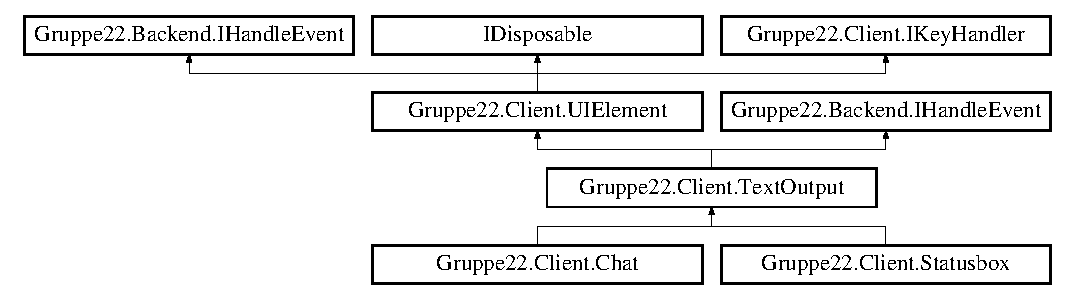
\includegraphics[height=3.589744cm]{class_gruppe22_1_1_client_1_1_text_output}
\end{center}
\end{figure}
\subsection*{Öffentliche Methoden}
\begin{DoxyCompactItemize}
\item 
virtual void \hyperlink{class_gruppe22_1_1_client_1_1_text_output_a1350976d5c45cef2d5227b5c4e097896}{Add\-Line} (string text, object color=null)
\begin{DoxyCompactList}\small\item\em Add a line of text to output (requires implementation in children \end{DoxyCompactList}\item 
\hyperlink{class_gruppe22_1_1_client_1_1_text_output_a7e08485e517fccfb2dbc1ed5507f40f2}{Text\-Output} (\hyperlink{interface_gruppe22_1_1_backend_1_1_i_handle_event}{Backend.\-I\-Handle\-Event} parent, Sprite\-Batch sprite\-Batch, Content\-Manager content, Rectangle display\-Rect)
\end{DoxyCompactItemize}
\subsection*{Weitere Geerbte Elemente}


\subsection{Ausführliche Beschreibung}
Class used for output -\/ parent to statusbox (output only) and chat (input + output) 



\subsection{Beschreibung der Konstruktoren und Destruktoren}
\hypertarget{class_gruppe22_1_1_client_1_1_text_output_a7e08485e517fccfb2dbc1ed5507f40f2}{\index{Gruppe22\-::\-Client\-::\-Text\-Output@{Gruppe22\-::\-Client\-::\-Text\-Output}!Text\-Output@{Text\-Output}}
\index{Text\-Output@{Text\-Output}!Gruppe22::Client::TextOutput@{Gruppe22\-::\-Client\-::\-Text\-Output}}
\subsubsection[{Text\-Output}]{\setlength{\rightskip}{0pt plus 5cm}Gruppe22.\-Client.\-Text\-Output.\-Text\-Output (
\begin{DoxyParamCaption}
\item[{{\bf Backend.\-I\-Handle\-Event}}]{parent, }
\item[{Sprite\-Batch}]{sprite\-Batch, }
\item[{Content\-Manager}]{content, }
\item[{Rectangle}]{display\-Rect}
\end{DoxyParamCaption}
)}}\label{class_gruppe22_1_1_client_1_1_text_output_a7e08485e517fccfb2dbc1ed5507f40f2}


\subsection{Dokumentation der Elementfunktionen}
\hypertarget{class_gruppe22_1_1_client_1_1_text_output_a1350976d5c45cef2d5227b5c4e097896}{\index{Gruppe22\-::\-Client\-::\-Text\-Output@{Gruppe22\-::\-Client\-::\-Text\-Output}!Add\-Line@{Add\-Line}}
\index{Add\-Line@{Add\-Line}!Gruppe22::Client::TextOutput@{Gruppe22\-::\-Client\-::\-Text\-Output}}
\subsubsection[{Add\-Line}]{\setlength{\rightskip}{0pt plus 5cm}virtual void Gruppe22.\-Client.\-Text\-Output.\-Add\-Line (
\begin{DoxyParamCaption}
\item[{string}]{text, }
\item[{object}]{color = {\ttfamily null}}
\end{DoxyParamCaption}
)\hspace{0.3cm}{\ttfamily [virtual]}}}\label{class_gruppe22_1_1_client_1_1_text_output_a1350976d5c45cef2d5227b5c4e097896}


Add a line of text to output (requires implementation in children 


\begin{DoxyParams}{Parameter}
{\em text} & \\
\hline
{\em color} & \\
\hline
\end{DoxyParams}


Erneute Implementation in \hyperlink{class_gruppe22_1_1_client_1_1_statusbox_a5b23e66c24de79d0a274577d63a6ad74}{Gruppe22.\-Client.\-Statusbox} und \hyperlink{class_gruppe22_1_1_client_1_1_chat_a4caef8eac20c6ac2094ca85de9ce2404}{Gruppe22.\-Client.\-Chat}.



Die Dokumentation für diese Klasse wurde erzeugt aufgrund der Datei\-:\begin{DoxyCompactItemize}
\item 
C\-:/\-Users/beursken/\-Documents/\-Git\-Hub/gruppe22/\-Gruppe22/\-Gruppe22/\-Client/\-U\-I/\hyperlink{_textoutput_8cs}{Textoutput.\-cs}\end{DoxyCompactItemize}

\hypertarget{class_gruppe22_1_1_client_1_1_texture_from_data}{\section{Gruppe22.\-Client.\-Texture\-From\-Data Klassenreferenz}
\label{class_gruppe22_1_1_client_1_1_texture_from_data}\index{Gruppe22.\-Client.\-Texture\-From\-Data@{Gruppe22.\-Client.\-Texture\-From\-Data}}
}
\subsection*{Öffentliche, statische Methoden}
\begin{DoxyCompactItemize}
\item 
static Texture2\-D \hyperlink{class_gruppe22_1_1_client_1_1_texture_from_data_a66cacb975b37a7db358a27c661e1558d}{Convert} (\hyperlink{class_gruppe22_1_1_backend_1_1_image_data}{Backend.\-Image\-Data} src, Content\-Manager content)
\end{DoxyCompactItemize}


\subsection{Dokumentation der Elementfunktionen}
\hypertarget{class_gruppe22_1_1_client_1_1_texture_from_data_a66cacb975b37a7db358a27c661e1558d}{\index{Gruppe22\-::\-Client\-::\-Texture\-From\-Data@{Gruppe22\-::\-Client\-::\-Texture\-From\-Data}!Convert@{Convert}}
\index{Convert@{Convert}!Gruppe22::Client::TextureFromData@{Gruppe22\-::\-Client\-::\-Texture\-From\-Data}}
\subsubsection[{Convert}]{\setlength{\rightskip}{0pt plus 5cm}static Texture2\-D Gruppe22.\-Client.\-Texture\-From\-Data.\-Convert (
\begin{DoxyParamCaption}
\item[{{\bf Backend.\-Image\-Data}}]{src, }
\item[{Content\-Manager}]{content}
\end{DoxyParamCaption}
)\hspace{0.3cm}{\ttfamily [static]}}}\label{class_gruppe22_1_1_client_1_1_texture_from_data_a66cacb975b37a7db358a27c661e1558d}


Die Dokumentation für diese Klasse wurde erzeugt aufgrund der Datei\-:\begin{DoxyCompactItemize}
\item 
C\-:/\-Users/beursken/\-Documents/\-Git\-Hub/gruppe22/\-Gruppe22/\-Gruppe22/\-Client/\-U\-I/\hyperlink{_image_info2_texture_8cs}{Image\-Info2\-Texture.\-cs}\end{DoxyCompactItemize}

\hypertarget{class_gruppe22_1_1_backend_1_1_tile}{\section{Gruppe22.\-Backend.\-Tile Klassenreferenz}
\label{class_gruppe22_1_1_backend_1_1_tile}\index{Gruppe22.\-Backend.\-Tile@{Gruppe22.\-Backend.\-Tile}}
}


An abstract class representing a generic tile (i.\-e. blank floor)  


Klassendiagramm für Gruppe22.\-Backend.\-Tile\-:\begin{figure}[H]
\begin{center}
\leavevmode
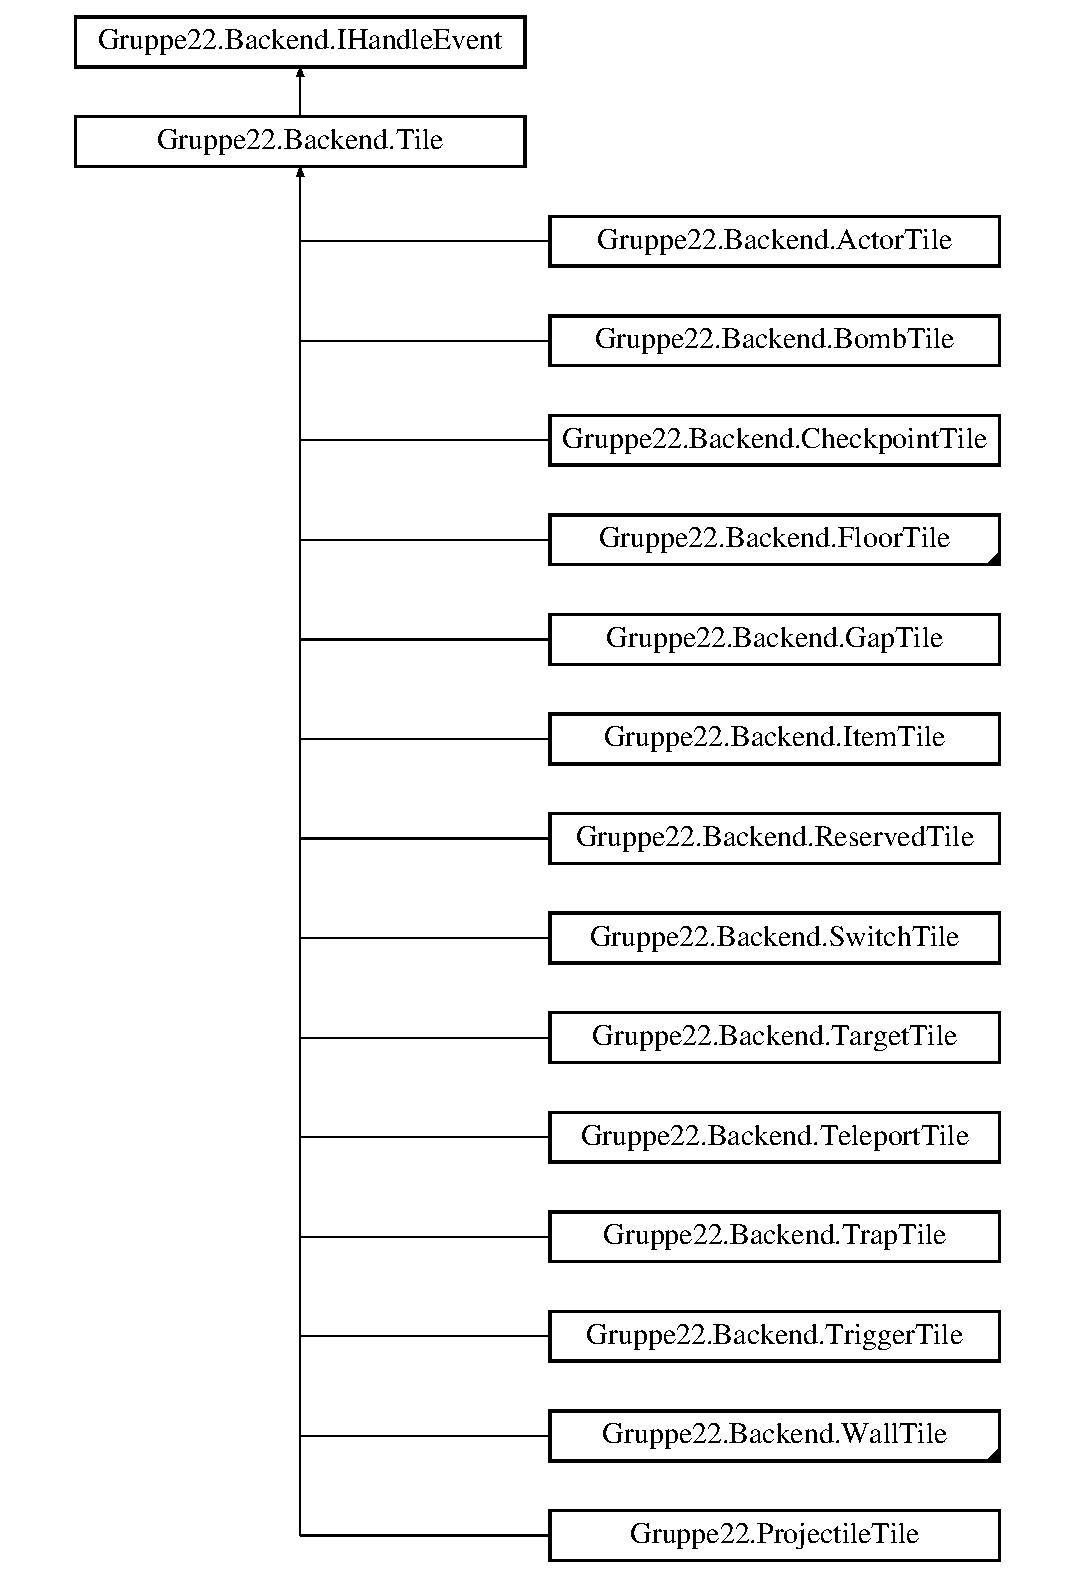
\includegraphics[height=12.000000cm]{class_gruppe22_1_1_backend_1_1_tile}
\end{center}
\end{figure}
\subsection*{Öffentliche Methoden}
\begin{DoxyCompactItemize}
\item 
virtual void \hyperlink{class_gruppe22_1_1_backend_1_1_tile_a0810154a52f859e852497e3717998e47}{Update} (Game\-Time game\-Time)
\item 
virtual void \hyperlink{class_gruppe22_1_1_backend_1_1_tile_a109ab3e77ffca9d44c95a711af3491dc}{Save} (Xml\-Writer xmlw)
\begin{DoxyCompactList}\small\item\em Abstract method to save a tile in a X\-M\-L file \end{DoxyCompactList}\item 
\hyperlink{class_gruppe22_1_1_backend_1_1_tile_aff91899925757cb0d274f3beaa51db79}{Tile} (object \hyperlink{class_gruppe22_1_1_backend_1_1_tile_abc12933c70eb3a2ebbb2fde9f45c2632}{parent})
\begin{DoxyCompactList}\small\item\em An empty constructor (setting default values) \end{DoxyCompactList}\item 
virtual void \hyperlink{class_gruppe22_1_1_backend_1_1_tile_a6bd5672c460c2e496dcaa483aa5e8438}{Handle\-Event} (bool Down\-Stream, \hyperlink{namespace_gruppe22_1_1_backend_ab56df91bb0bdafa1ea978e552209ce73}{Events} event\-I\-D, params object\mbox{[}$\,$\mbox{]} data)
\end{DoxyCompactItemize}
\subsection*{Geschützte Attribute}
\begin{DoxyCompactItemize}
\item 
object \hyperlink{class_gruppe22_1_1_backend_1_1_tile_aee3960c872a95f378086b1655caddbcb}{\-\_\-parent} = null
\end{DoxyCompactItemize}
\subsection*{Propertys}
\begin{DoxyCompactItemize}
\item 
\hyperlink{class_gruppe22_1_1_backend_1_1_coords}{Backend.\-Coords} \hyperlink{class_gruppe22_1_1_backend_1_1_tile_a0fd463d0eb3f37522d0e4ff6692b9fcd}{coords}\hspace{0.3cm}{\ttfamily  \mbox{[}get, set\mbox{]}}
\item 
object \hyperlink{class_gruppe22_1_1_backend_1_1_tile_abc12933c70eb3a2ebbb2fde9f45c2632}{parent}\hspace{0.3cm}{\ttfamily  \mbox{[}get, set\mbox{]}}
\end{DoxyCompactItemize}


\subsection{Ausführliche Beschreibung}
An abstract class representing a generic tile (i.\-e. blank floor) 



\subsection{Beschreibung der Konstruktoren und Destruktoren}
\hypertarget{class_gruppe22_1_1_backend_1_1_tile_aff91899925757cb0d274f3beaa51db79}{\index{Gruppe22\-::\-Backend\-::\-Tile@{Gruppe22\-::\-Backend\-::\-Tile}!Tile@{Tile}}
\index{Tile@{Tile}!Gruppe22::Backend::Tile@{Gruppe22\-::\-Backend\-::\-Tile}}
\subsubsection[{Tile}]{\setlength{\rightskip}{0pt plus 5cm}Gruppe22.\-Backend.\-Tile.\-Tile (
\begin{DoxyParamCaption}
\item[{object}]{parent}
\end{DoxyParamCaption}
)}}\label{class_gruppe22_1_1_backend_1_1_tile_aff91899925757cb0d274f3beaa51db79}


An empty constructor (setting default values) 



\subsection{Dokumentation der Elementfunktionen}
\hypertarget{class_gruppe22_1_1_backend_1_1_tile_a6bd5672c460c2e496dcaa483aa5e8438}{\index{Gruppe22\-::\-Backend\-::\-Tile@{Gruppe22\-::\-Backend\-::\-Tile}!Handle\-Event@{Handle\-Event}}
\index{Handle\-Event@{Handle\-Event}!Gruppe22::Backend::Tile@{Gruppe22\-::\-Backend\-::\-Tile}}
\subsubsection[{Handle\-Event}]{\setlength{\rightskip}{0pt plus 5cm}virtual void Gruppe22.\-Backend.\-Tile.\-Handle\-Event (
\begin{DoxyParamCaption}
\item[{bool}]{Down\-Stream, }
\item[{{\bf Events}}]{event\-I\-D, }
\item[{params object\mbox{[}$\,$\mbox{]}}]{data}
\end{DoxyParamCaption}
)\hspace{0.3cm}{\ttfamily [virtual]}}}\label{class_gruppe22_1_1_backend_1_1_tile_a6bd5672c460c2e496dcaa483aa5e8438}
\hypertarget{class_gruppe22_1_1_backend_1_1_tile_a109ab3e77ffca9d44c95a711af3491dc}{\index{Gruppe22\-::\-Backend\-::\-Tile@{Gruppe22\-::\-Backend\-::\-Tile}!Save@{Save}}
\index{Save@{Save}!Gruppe22::Backend::Tile@{Gruppe22\-::\-Backend\-::\-Tile}}
\subsubsection[{Save}]{\setlength{\rightskip}{0pt plus 5cm}virtual void Gruppe22.\-Backend.\-Tile.\-Save (
\begin{DoxyParamCaption}
\item[{Xml\-Writer}]{xmlw}
\end{DoxyParamCaption}
)\hspace{0.3cm}{\ttfamily [virtual]}}}\label{class_gruppe22_1_1_backend_1_1_tile_a109ab3e77ffca9d44c95a711af3491dc}


Abstract method to save a tile in a X\-M\-L file 


\begin{DoxyParams}{Parameter}
{\em xmlw} & the Xml\-Writer used for saving the file\\
\hline
\end{DoxyParams}


Erneute Implementation in \hyperlink{class_gruppe22_1_1_backend_1_1_floor_tile_a4a096b8d6ff25557bd807751268987f2}{Gruppe22.\-Backend.\-Floor\-Tile}, \hyperlink{class_gruppe22_1_1_backend_1_1_trap_tile_a923a400fdf039c83ef4e6c3a42170b73}{Gruppe22.\-Backend.\-Trap\-Tile}, \hyperlink{class_gruppe22_1_1_backend_1_1_trigger_tile_a218716e27c1c692f05e0b538b30dcc59}{Gruppe22.\-Backend.\-Trigger\-Tile}, \hyperlink{class_gruppe22_1_1_backend_1_1_teleport_tile_a15a8abf308bcb1577fdea70a4959bf79}{Gruppe22.\-Backend.\-Teleport\-Tile}, \hyperlink{class_gruppe22_1_1_backend_1_1_wall_tile_affcf30d6a5d46d74c8c570bb83cf99f8}{Gruppe22.\-Backend.\-Wall\-Tile}, \hyperlink{class_gruppe22_1_1_backend_1_1_reserved_tile_a394fda5eebd1e5c853c904979bbe04ea}{Gruppe22.\-Backend.\-Reserved\-Tile}, \hyperlink{class_gruppe22_1_1_projectile_tile_ac04e7d0bab385f083a1d4dca56083f3d}{Gruppe22.\-Projectile\-Tile}, \hyperlink{class_gruppe22_1_1_backend_1_1_switch_tile_aa50a0cf7dde944e73b9b2640042e78d2}{Gruppe22.\-Backend.\-Switch\-Tile}, \hyperlink{class_gruppe22_1_1_backend_1_1_actor_tile_aad98091f10ca75642d211c1a837141e4}{Gruppe22.\-Backend.\-Actor\-Tile}, \hyperlink{class_gruppe22_1_1_backend_1_1_door_tile_a89bddd70828e64c6491d92a225db0474}{Gruppe22.\-Backend.\-Door\-Tile}, \hyperlink{class_gruppe22_1_1_backend_1_1_item_tile_a2e58e18ae35c42b311fcdaa1664ec505}{Gruppe22.\-Backend.\-Item\-Tile}, \hyperlink{class_gruppe22_1_1_backend_1_1_gap_tile_aeeed4e7d3d3d230ba20398bee17f4ed2}{Gruppe22.\-Backend.\-Gap\-Tile} und \hyperlink{class_gruppe22_1_1_backend_1_1_target_tile_a3bb3f1712e44d11503f5da8226cba9f6}{Gruppe22.\-Backend.\-Target\-Tile}.

\hypertarget{class_gruppe22_1_1_backend_1_1_tile_a0810154a52f859e852497e3717998e47}{\index{Gruppe22\-::\-Backend\-::\-Tile@{Gruppe22\-::\-Backend\-::\-Tile}!Update@{Update}}
\index{Update@{Update}!Gruppe22::Backend::Tile@{Gruppe22\-::\-Backend\-::\-Tile}}
\subsubsection[{Update}]{\setlength{\rightskip}{0pt plus 5cm}virtual void Gruppe22.\-Backend.\-Tile.\-Update (
\begin{DoxyParamCaption}
\item[{Game\-Time}]{game\-Time}
\end{DoxyParamCaption}
)\hspace{0.3cm}{\ttfamily [virtual]}}}\label{class_gruppe22_1_1_backend_1_1_tile_a0810154a52f859e852497e3717998e47}


Erneute Implementation in \hyperlink{class_gruppe22_1_1_backend_1_1_floor_tile_ae3d0627204d49dabc8180fd0bdd22803}{Gruppe22.\-Backend.\-Floor\-Tile}.



\subsection{Dokumentation der Datenelemente}
\hypertarget{class_gruppe22_1_1_backend_1_1_tile_aee3960c872a95f378086b1655caddbcb}{\index{Gruppe22\-::\-Backend\-::\-Tile@{Gruppe22\-::\-Backend\-::\-Tile}!\-\_\-parent@{\-\_\-parent}}
\index{\-\_\-parent@{\-\_\-parent}!Gruppe22::Backend::Tile@{Gruppe22\-::\-Backend\-::\-Tile}}
\subsubsection[{\-\_\-parent}]{\setlength{\rightskip}{0pt plus 5cm}object Gruppe22.\-Backend.\-Tile.\-\_\-parent = null\hspace{0.3cm}{\ttfamily [protected]}}}\label{class_gruppe22_1_1_backend_1_1_tile_aee3960c872a95f378086b1655caddbcb}


\subsection{Dokumentation der Propertys}
\hypertarget{class_gruppe22_1_1_backend_1_1_tile_a0fd463d0eb3f37522d0e4ff6692b9fcd}{\index{Gruppe22\-::\-Backend\-::\-Tile@{Gruppe22\-::\-Backend\-::\-Tile}!coords@{coords}}
\index{coords@{coords}!Gruppe22::Backend::Tile@{Gruppe22\-::\-Backend\-::\-Tile}}
\subsubsection[{coords}]{\setlength{\rightskip}{0pt plus 5cm}{\bf Backend.\-Coords} Gruppe22.\-Backend.\-Tile.\-coords\hspace{0.3cm}{\ttfamily [get]}, {\ttfamily [set]}}}\label{class_gruppe22_1_1_backend_1_1_tile_a0fd463d0eb3f37522d0e4ff6692b9fcd}
\hypertarget{class_gruppe22_1_1_backend_1_1_tile_abc12933c70eb3a2ebbb2fde9f45c2632}{\index{Gruppe22\-::\-Backend\-::\-Tile@{Gruppe22\-::\-Backend\-::\-Tile}!parent@{parent}}
\index{parent@{parent}!Gruppe22::Backend::Tile@{Gruppe22\-::\-Backend\-::\-Tile}}
\subsubsection[{parent}]{\setlength{\rightskip}{0pt plus 5cm}object Gruppe22.\-Backend.\-Tile.\-parent\hspace{0.3cm}{\ttfamily [get]}, {\ttfamily [set]}}}\label{class_gruppe22_1_1_backend_1_1_tile_abc12933c70eb3a2ebbb2fde9f45c2632}


Die Dokumentation für diese Klasse wurde erzeugt aufgrund der Datei\-:\begin{DoxyCompactItemize}
\item 
C\-:/\-Users/beursken/\-Documents/\-Git\-Hub/gruppe22/\-Gruppe22/\-Gruppe22/\-Backend/\-Map/\hyperlink{_tile_8cs}{Tile.\-cs}\end{DoxyCompactItemize}

\hypertarget{class_gruppe22_1_1_client_1_1_tile_object}{\section{Gruppe22.\-Client.\-Tile\-Object Klassenreferenz}
\label{class_gruppe22_1_1_client_1_1_tile_object}\index{Gruppe22.\-Client.\-Tile\-Object@{Gruppe22.\-Client.\-Tile\-Object}}
}


All animations used in displaying a specific tile  


Klassendiagramm für Gruppe22.\-Client.\-Tile\-Object\-:\begin{figure}[H]
\begin{center}
\leavevmode
\includegraphics[height=2.000000cm]{class_gruppe22_1_1_client_1_1_tile_object}
\end{center}
\end{figure}
\subsection*{Öffentliche Methoden}
\begin{DoxyCompactItemize}
\item 
bool \hyperlink{class_gruppe22_1_1_client_1_1_tile_object_a73d2b8e84dd9f8ec02a74cc122bd61f2}{Next\-Animation} ()
\begin{DoxyCompactList}\small\item\em Loop animation to next frame \end{DoxyCompactList}\item 
void \hyperlink{class_gruppe22_1_1_client_1_1_tile_object_a31fe95c4ae53e15acacb245a35690d72}{Reset\-Animation} ()
\begin{DoxyCompactList}\small\item\em Restart current animation at first frame \end{DoxyCompactList}\item 
void \hyperlink{class_gruppe22_1_1_client_1_1_tile_object_ab807224e88c66c53e8ca355e1dc88ee6}{Final\-Animation} ()
\begin{DoxyCompactList}\small\item\em Show the final phase of the animation \end{DoxyCompactList}\item 
void \hyperlink{class_gruppe22_1_1_client_1_1_tile_object_a87b07352fbf1a1ed6ed283c4f390d785}{Add\-Animation} (string src, \hyperlink{class_gruppe22_1_1_backend_1_1_coords}{Backend.\-Coords} start, int cols=1, int rows=1, \hyperlink{class_gruppe22_1_1_backend_1_1_coords}{Backend.\-Coords} offset=null, \hyperlink{class_gruppe22_1_1_backend_1_1_coords}{Backend.\-Coords} crop=null, bool order=false)
\begin{DoxyCompactList}\small\item\em Add multiple animation phases from a single file \end{DoxyCompactList}\item 
\hyperlink{class_gruppe22_1_1_client_1_1_tile_object_a8d869a4075b393c7bb3e6728e6be439d}{Tile\-Object} (Content\-Manager content, int \hyperlink{class_gruppe22_1_1_client_1_1_tile_object_ad12970584aeb4e8ddcc748cbd24e11bd}{width}=128, int \hyperlink{class_gruppe22_1_1_client_1_1_tile_object_a6bfc3a726f20db8d708c172cf5488df9}{height}=192)
\item 
\hyperlink{class_gruppe22_1_1_client_1_1_tile_object_acb85b1d844b7d2d77d7c43ddd9b991ed}{Tile\-Object} ()
\item 
System.\-Xml.\-Schema.\-Xml\-Schema \hyperlink{class_gruppe22_1_1_client_1_1_tile_object_ab7ffb591c1031161c6b986a1de374cc4}{Get\-Schema} ()
\begin{DoxyCompactList}\small\item\em Useless function from the I\-Xml\-Serializable-\/\-Interface \end{DoxyCompactList}\item 
void \hyperlink{class_gruppe22_1_1_client_1_1_tile_object_a5c2e19f632fe0524448e77604ad0653a}{Read\-Xml} (System.\-Xml.\-Xml\-Reader reader)
\begin{DoxyCompactList}\small\item\em Get X\-M\-L-\/data from a file \end{DoxyCompactList}\item 
void \hyperlink{class_gruppe22_1_1_client_1_1_tile_object_abed9b73a739881a1fa04fcb4cd323df2}{Write\-Xml} (System.\-Xml.\-Xml\-Writer writer)
\begin{DoxyCompactList}\small\item\em Dump the whole group of animations to an X\-M\-L-\/file \end{DoxyCompactList}\end{DoxyCompactItemize}
\subsection*{Propertys}
\begin{DoxyCompactItemize}
\item 
bool \hyperlink{class_gruppe22_1_1_client_1_1_tile_object_aac8f058e227f664c4f5b930ee3b0bef4}{loop}\hspace{0.3cm}{\ttfamily  \mbox{[}get, set\mbox{]}}
\begin{DoxyCompactList}\small\item\em true if the current animation loops (i.\-e. repeats endlessly) \end{DoxyCompactList}\item 
int \hyperlink{class_gruppe22_1_1_client_1_1_tile_object_aca5785e249ae405b4c83551cd679e6bb}{offset\-X}\hspace{0.3cm}{\ttfamily  \mbox{[}get, set\mbox{]}}
\item 
int \hyperlink{class_gruppe22_1_1_client_1_1_tile_object_a747e38501941605465e87c10c1f0dec3}{offset\-Y}\hspace{0.3cm}{\ttfamily  \mbox{[}get, set\mbox{]}}
\item 
int \hyperlink{class_gruppe22_1_1_client_1_1_tile_object_a27b17807e321cc1c815b4836e056f12d}{crop\-X}\hspace{0.3cm}{\ttfamily  \mbox{[}get, set\mbox{]}}
\item 
int \hyperlink{class_gruppe22_1_1_client_1_1_tile_object_aa8317bc2ecd752a925526c909f9c373a}{crop\-Y}\hspace{0.3cm}{\ttfamily  \mbox{[}get, set\mbox{]}}
\item 
bool \hyperlink{class_gruppe22_1_1_client_1_1_tile_object_adcf3bc51e88b76fd550b8d23202d55e4}{is\-Valid}\hspace{0.3cm}{\ttfamily  \mbox{[}get\mbox{]}}
\begin{DoxyCompactList}\small\item\em True if we can return a valid bitmap \end{DoxyCompactList}\item 
string \hyperlink{class_gruppe22_1_1_client_1_1_tile_object_adeaefcb12857798290d66adc39ce19aa}{animation\-File}\hspace{0.3cm}{\ttfamily  \mbox{[}get, set\mbox{]}}
\begin{DoxyCompactList}\small\item\em The file containing the current animation phase \end{DoxyCompactList}\item 
Texture2\-D \hyperlink{class_gruppe22_1_1_client_1_1_tile_object_a4f7a5bb65030d656eb6e5755bb4678aa}{animation\-Texture}\hspace{0.3cm}{\ttfamily  \mbox{[}get\mbox{]}}
\begin{DoxyCompactList}\small\item\em A bitmap containing the current animation phase \end{DoxyCompactList}\item 
int \hyperlink{class_gruppe22_1_1_client_1_1_tile_object_a6ad718b3f74074c310a6530d20d0c3c9}{animation\-I\-D}\hspace{0.3cm}{\ttfamily  \mbox{[}get\mbox{]}}
\item 
Rectangle \hyperlink{class_gruppe22_1_1_client_1_1_tile_object_ad68010b4b4677968177f6d6ab0b26324}{animation\-Rect}\hspace{0.3cm}{\ttfamily  \mbox{[}get, set\mbox{]}}
\begin{DoxyCompactList}\small\item\em The rectangle used to cut out the current animation phase \end{DoxyCompactList}\item 
int \hyperlink{class_gruppe22_1_1_client_1_1_tile_object_a6bfc3a726f20db8d708c172cf5488df9}{height}\hspace{0.3cm}{\ttfamily  \mbox{[}get, set\mbox{]}}
\item 
int \hyperlink{class_gruppe22_1_1_client_1_1_tile_object_ad12970584aeb4e8ddcc748cbd24e11bd}{width}\hspace{0.3cm}{\ttfamily  \mbox{[}get, set\mbox{]}}
\end{DoxyCompactItemize}


\subsection{Ausführliche Beschreibung}
All animations used in displaying a specific tile 



\subsection{Beschreibung der Konstruktoren und Destruktoren}
\hypertarget{class_gruppe22_1_1_client_1_1_tile_object_a8d869a4075b393c7bb3e6728e6be439d}{\index{Gruppe22\-::\-Client\-::\-Tile\-Object@{Gruppe22\-::\-Client\-::\-Tile\-Object}!Tile\-Object@{Tile\-Object}}
\index{Tile\-Object@{Tile\-Object}!Gruppe22::Client::TileObject@{Gruppe22\-::\-Client\-::\-Tile\-Object}}
\subsubsection[{Tile\-Object}]{\setlength{\rightskip}{0pt plus 5cm}Gruppe22.\-Client.\-Tile\-Object.\-Tile\-Object (
\begin{DoxyParamCaption}
\item[{Content\-Manager}]{content, }
\item[{int}]{width = {\ttfamily 128}, }
\item[{int}]{height = {\ttfamily 192}}
\end{DoxyParamCaption}
)}}\label{class_gruppe22_1_1_client_1_1_tile_object_a8d869a4075b393c7bb3e6728e6be439d}





\begin{DoxyParams}{Parameter}
{\em width} & \\
\hline
{\em height} & \\
\hline
{\em animations} & \\
\hline
\end{DoxyParams}
\hypertarget{class_gruppe22_1_1_client_1_1_tile_object_acb85b1d844b7d2d77d7c43ddd9b991ed}{\index{Gruppe22\-::\-Client\-::\-Tile\-Object@{Gruppe22\-::\-Client\-::\-Tile\-Object}!Tile\-Object@{Tile\-Object}}
\index{Tile\-Object@{Tile\-Object}!Gruppe22::Client::TileObject@{Gruppe22\-::\-Client\-::\-Tile\-Object}}
\subsubsection[{Tile\-Object}]{\setlength{\rightskip}{0pt plus 5cm}Gruppe22.\-Client.\-Tile\-Object.\-Tile\-Object (
\begin{DoxyParamCaption}
{}
\end{DoxyParamCaption}
)}}\label{class_gruppe22_1_1_client_1_1_tile_object_acb85b1d844b7d2d77d7c43ddd9b991ed}


\subsection{Dokumentation der Elementfunktionen}
\hypertarget{class_gruppe22_1_1_client_1_1_tile_object_a87b07352fbf1a1ed6ed283c4f390d785}{\index{Gruppe22\-::\-Client\-::\-Tile\-Object@{Gruppe22\-::\-Client\-::\-Tile\-Object}!Add\-Animation@{Add\-Animation}}
\index{Add\-Animation@{Add\-Animation}!Gruppe22::Client::TileObject@{Gruppe22\-::\-Client\-::\-Tile\-Object}}
\subsubsection[{Add\-Animation}]{\setlength{\rightskip}{0pt plus 5cm}void Gruppe22.\-Client.\-Tile\-Object.\-Add\-Animation (
\begin{DoxyParamCaption}
\item[{string}]{src, }
\item[{{\bf Backend.\-Coords}}]{start, }
\item[{int}]{cols = {\ttfamily 1}, }
\item[{int}]{rows = {\ttfamily 1}, }
\item[{{\bf Backend.\-Coords}}]{offset = {\ttfamily null}, }
\item[{{\bf Backend.\-Coords}}]{crop = {\ttfamily null}, }
\item[{bool}]{order = {\ttfamily false}}
\end{DoxyParamCaption}
)}}\label{class_gruppe22_1_1_client_1_1_tile_object_a87b07352fbf1a1ed6ed283c4f390d785}


Add multiple animation phases from a single file 


\begin{DoxyParams}{Parameter}
{\em animation} & \\
\hline
{\em src} & Source File\\
\hline
{\em start} & T\-Op left corner of first frame (width and height determined by animation object!)\\
\hline
{\em cols} & Number of columns used in the animation\\
\hline
{\em rows} & Number of rows used in the animation\\
\hline
{\em order} & Whether to read row by row (false, default) or column by column (true)\\
\hline
\end{DoxyParams}
\begin{DoxyReturn}{Rückgabe}
I\-D of Animation added to or -\/1 if invalid target was passed
\end{DoxyReturn}
\hypertarget{class_gruppe22_1_1_client_1_1_tile_object_ab807224e88c66c53e8ca355e1dc88ee6}{\index{Gruppe22\-::\-Client\-::\-Tile\-Object@{Gruppe22\-::\-Client\-::\-Tile\-Object}!Final\-Animation@{Final\-Animation}}
\index{Final\-Animation@{Final\-Animation}!Gruppe22::Client::TileObject@{Gruppe22\-::\-Client\-::\-Tile\-Object}}
\subsubsection[{Final\-Animation}]{\setlength{\rightskip}{0pt plus 5cm}void Gruppe22.\-Client.\-Tile\-Object.\-Final\-Animation (
\begin{DoxyParamCaption}
{}
\end{DoxyParamCaption}
)}}\label{class_gruppe22_1_1_client_1_1_tile_object_ab807224e88c66c53e8ca355e1dc88ee6}


Show the final phase of the animation 

\hypertarget{class_gruppe22_1_1_client_1_1_tile_object_ab7ffb591c1031161c6b986a1de374cc4}{\index{Gruppe22\-::\-Client\-::\-Tile\-Object@{Gruppe22\-::\-Client\-::\-Tile\-Object}!Get\-Schema@{Get\-Schema}}
\index{Get\-Schema@{Get\-Schema}!Gruppe22::Client::TileObject@{Gruppe22\-::\-Client\-::\-Tile\-Object}}
\subsubsection[{Get\-Schema}]{\setlength{\rightskip}{0pt plus 5cm}System.\-Xml.\-Schema.\-Xml\-Schema Gruppe22.\-Client.\-Tile\-Object.\-Get\-Schema (
\begin{DoxyParamCaption}
{}
\end{DoxyParamCaption}
)}}\label{class_gruppe22_1_1_client_1_1_tile_object_ab7ffb591c1031161c6b986a1de374cc4}


Useless function from the I\-Xml\-Serializable-\/\-Interface 

\begin{DoxyReturn}{Rückgabe}
null
\end{DoxyReturn}
\hypertarget{class_gruppe22_1_1_client_1_1_tile_object_a73d2b8e84dd9f8ec02a74cc122bd61f2}{\index{Gruppe22\-::\-Client\-::\-Tile\-Object@{Gruppe22\-::\-Client\-::\-Tile\-Object}!Next\-Animation@{Next\-Animation}}
\index{Next\-Animation@{Next\-Animation}!Gruppe22::Client::TileObject@{Gruppe22\-::\-Client\-::\-Tile\-Object}}
\subsubsection[{Next\-Animation}]{\setlength{\rightskip}{0pt plus 5cm}bool Gruppe22.\-Client.\-Tile\-Object.\-Next\-Animation (
\begin{DoxyParamCaption}
{}
\end{DoxyParamCaption}
)}}\label{class_gruppe22_1_1_client_1_1_tile_object_a73d2b8e84dd9f8ec02a74cc122bd61f2}


Loop animation to next frame 

\hypertarget{class_gruppe22_1_1_client_1_1_tile_object_a5c2e19f632fe0524448e77604ad0653a}{\index{Gruppe22\-::\-Client\-::\-Tile\-Object@{Gruppe22\-::\-Client\-::\-Tile\-Object}!Read\-Xml@{Read\-Xml}}
\index{Read\-Xml@{Read\-Xml}!Gruppe22::Client::TileObject@{Gruppe22\-::\-Client\-::\-Tile\-Object}}
\subsubsection[{Read\-Xml}]{\setlength{\rightskip}{0pt plus 5cm}void Gruppe22.\-Client.\-Tile\-Object.\-Read\-Xml (
\begin{DoxyParamCaption}
\item[{System.\-Xml.\-Xml\-Reader}]{reader}
\end{DoxyParamCaption}
)}}\label{class_gruppe22_1_1_client_1_1_tile_object_a5c2e19f632fe0524448e77604ad0653a}


Get X\-M\-L-\/data from a file 


\begin{DoxyParams}{Parameter}
{\em reader} & The file from which data will be read\\
\hline
\end{DoxyParams}
\hypertarget{class_gruppe22_1_1_client_1_1_tile_object_a31fe95c4ae53e15acacb245a35690d72}{\index{Gruppe22\-::\-Client\-::\-Tile\-Object@{Gruppe22\-::\-Client\-::\-Tile\-Object}!Reset\-Animation@{Reset\-Animation}}
\index{Reset\-Animation@{Reset\-Animation}!Gruppe22::Client::TileObject@{Gruppe22\-::\-Client\-::\-Tile\-Object}}
\subsubsection[{Reset\-Animation}]{\setlength{\rightskip}{0pt plus 5cm}void Gruppe22.\-Client.\-Tile\-Object.\-Reset\-Animation (
\begin{DoxyParamCaption}
{}
\end{DoxyParamCaption}
)}}\label{class_gruppe22_1_1_client_1_1_tile_object_a31fe95c4ae53e15acacb245a35690d72}


Restart current animation at first frame 

\hypertarget{class_gruppe22_1_1_client_1_1_tile_object_abed9b73a739881a1fa04fcb4cd323df2}{\index{Gruppe22\-::\-Client\-::\-Tile\-Object@{Gruppe22\-::\-Client\-::\-Tile\-Object}!Write\-Xml@{Write\-Xml}}
\index{Write\-Xml@{Write\-Xml}!Gruppe22::Client::TileObject@{Gruppe22\-::\-Client\-::\-Tile\-Object}}
\subsubsection[{Write\-Xml}]{\setlength{\rightskip}{0pt plus 5cm}void Gruppe22.\-Client.\-Tile\-Object.\-Write\-Xml (
\begin{DoxyParamCaption}
\item[{System.\-Xml.\-Xml\-Writer}]{writer}
\end{DoxyParamCaption}
)}}\label{class_gruppe22_1_1_client_1_1_tile_object_abed9b73a739881a1fa04fcb4cd323df2}


Dump the whole group of animations to an X\-M\-L-\/file 


\begin{DoxyParams}{Parameter}
{\em writer} & The file used to write the data\\
\hline
\end{DoxyParams}


\subsection{Dokumentation der Propertys}
\hypertarget{class_gruppe22_1_1_client_1_1_tile_object_adeaefcb12857798290d66adc39ce19aa}{\index{Gruppe22\-::\-Client\-::\-Tile\-Object@{Gruppe22\-::\-Client\-::\-Tile\-Object}!animation\-File@{animation\-File}}
\index{animation\-File@{animation\-File}!Gruppe22::Client::TileObject@{Gruppe22\-::\-Client\-::\-Tile\-Object}}
\subsubsection[{animation\-File}]{\setlength{\rightskip}{0pt plus 5cm}string Gruppe22.\-Client.\-Tile\-Object.\-animation\-File\hspace{0.3cm}{\ttfamily [get]}, {\ttfamily [set]}}}\label{class_gruppe22_1_1_client_1_1_tile_object_adeaefcb12857798290d66adc39ce19aa}


The file containing the current animation phase 

\hypertarget{class_gruppe22_1_1_client_1_1_tile_object_a6ad718b3f74074c310a6530d20d0c3c9}{\index{Gruppe22\-::\-Client\-::\-Tile\-Object@{Gruppe22\-::\-Client\-::\-Tile\-Object}!animation\-I\-D@{animation\-I\-D}}
\index{animation\-I\-D@{animation\-I\-D}!Gruppe22::Client::TileObject@{Gruppe22\-::\-Client\-::\-Tile\-Object}}
\subsubsection[{animation\-I\-D}]{\setlength{\rightskip}{0pt plus 5cm}int Gruppe22.\-Client.\-Tile\-Object.\-animation\-I\-D\hspace{0.3cm}{\ttfamily [get]}}}\label{class_gruppe22_1_1_client_1_1_tile_object_a6ad718b3f74074c310a6530d20d0c3c9}
\hypertarget{class_gruppe22_1_1_client_1_1_tile_object_ad68010b4b4677968177f6d6ab0b26324}{\index{Gruppe22\-::\-Client\-::\-Tile\-Object@{Gruppe22\-::\-Client\-::\-Tile\-Object}!animation\-Rect@{animation\-Rect}}
\index{animation\-Rect@{animation\-Rect}!Gruppe22::Client::TileObject@{Gruppe22\-::\-Client\-::\-Tile\-Object}}
\subsubsection[{animation\-Rect}]{\setlength{\rightskip}{0pt plus 5cm}Rectangle Gruppe22.\-Client.\-Tile\-Object.\-animation\-Rect\hspace{0.3cm}{\ttfamily [get]}, {\ttfamily [set]}}}\label{class_gruppe22_1_1_client_1_1_tile_object_ad68010b4b4677968177f6d6ab0b26324}


The rectangle used to cut out the current animation phase 

\hypertarget{class_gruppe22_1_1_client_1_1_tile_object_a4f7a5bb65030d656eb6e5755bb4678aa}{\index{Gruppe22\-::\-Client\-::\-Tile\-Object@{Gruppe22\-::\-Client\-::\-Tile\-Object}!animation\-Texture@{animation\-Texture}}
\index{animation\-Texture@{animation\-Texture}!Gruppe22::Client::TileObject@{Gruppe22\-::\-Client\-::\-Tile\-Object}}
\subsubsection[{animation\-Texture}]{\setlength{\rightskip}{0pt plus 5cm}Texture2\-D Gruppe22.\-Client.\-Tile\-Object.\-animation\-Texture\hspace{0.3cm}{\ttfamily [get]}}}\label{class_gruppe22_1_1_client_1_1_tile_object_a4f7a5bb65030d656eb6e5755bb4678aa}


A bitmap containing the current animation phase 

\hypertarget{class_gruppe22_1_1_client_1_1_tile_object_a27b17807e321cc1c815b4836e056f12d}{\index{Gruppe22\-::\-Client\-::\-Tile\-Object@{Gruppe22\-::\-Client\-::\-Tile\-Object}!crop\-X@{crop\-X}}
\index{crop\-X@{crop\-X}!Gruppe22::Client::TileObject@{Gruppe22\-::\-Client\-::\-Tile\-Object}}
\subsubsection[{crop\-X}]{\setlength{\rightskip}{0pt plus 5cm}int Gruppe22.\-Client.\-Tile\-Object.\-crop\-X\hspace{0.3cm}{\ttfamily [get]}, {\ttfamily [set]}}}\label{class_gruppe22_1_1_client_1_1_tile_object_a27b17807e321cc1c815b4836e056f12d}
\hypertarget{class_gruppe22_1_1_client_1_1_tile_object_aa8317bc2ecd752a925526c909f9c373a}{\index{Gruppe22\-::\-Client\-::\-Tile\-Object@{Gruppe22\-::\-Client\-::\-Tile\-Object}!crop\-Y@{crop\-Y}}
\index{crop\-Y@{crop\-Y}!Gruppe22::Client::TileObject@{Gruppe22\-::\-Client\-::\-Tile\-Object}}
\subsubsection[{crop\-Y}]{\setlength{\rightskip}{0pt plus 5cm}int Gruppe22.\-Client.\-Tile\-Object.\-crop\-Y\hspace{0.3cm}{\ttfamily [get]}, {\ttfamily [set]}}}\label{class_gruppe22_1_1_client_1_1_tile_object_aa8317bc2ecd752a925526c909f9c373a}
\hypertarget{class_gruppe22_1_1_client_1_1_tile_object_a6bfc3a726f20db8d708c172cf5488df9}{\index{Gruppe22\-::\-Client\-::\-Tile\-Object@{Gruppe22\-::\-Client\-::\-Tile\-Object}!height@{height}}
\index{height@{height}!Gruppe22::Client::TileObject@{Gruppe22\-::\-Client\-::\-Tile\-Object}}
\subsubsection[{height}]{\setlength{\rightskip}{0pt plus 5cm}int Gruppe22.\-Client.\-Tile\-Object.\-height\hspace{0.3cm}{\ttfamily [get]}, {\ttfamily [set]}}}\label{class_gruppe22_1_1_client_1_1_tile_object_a6bfc3a726f20db8d708c172cf5488df9}
\hypertarget{class_gruppe22_1_1_client_1_1_tile_object_adcf3bc51e88b76fd550b8d23202d55e4}{\index{Gruppe22\-::\-Client\-::\-Tile\-Object@{Gruppe22\-::\-Client\-::\-Tile\-Object}!is\-Valid@{is\-Valid}}
\index{is\-Valid@{is\-Valid}!Gruppe22::Client::TileObject@{Gruppe22\-::\-Client\-::\-Tile\-Object}}
\subsubsection[{is\-Valid}]{\setlength{\rightskip}{0pt plus 5cm}bool Gruppe22.\-Client.\-Tile\-Object.\-is\-Valid\hspace{0.3cm}{\ttfamily [get]}}}\label{class_gruppe22_1_1_client_1_1_tile_object_adcf3bc51e88b76fd550b8d23202d55e4}


True if we can return a valid bitmap 

\hypertarget{class_gruppe22_1_1_client_1_1_tile_object_aac8f058e227f664c4f5b930ee3b0bef4}{\index{Gruppe22\-::\-Client\-::\-Tile\-Object@{Gruppe22\-::\-Client\-::\-Tile\-Object}!loop@{loop}}
\index{loop@{loop}!Gruppe22::Client::TileObject@{Gruppe22\-::\-Client\-::\-Tile\-Object}}
\subsubsection[{loop}]{\setlength{\rightskip}{0pt plus 5cm}bool Gruppe22.\-Client.\-Tile\-Object.\-loop\hspace{0.3cm}{\ttfamily [get]}, {\ttfamily [set]}}}\label{class_gruppe22_1_1_client_1_1_tile_object_aac8f058e227f664c4f5b930ee3b0bef4}


true if the current animation loops (i.\-e. repeats endlessly) 

\hypertarget{class_gruppe22_1_1_client_1_1_tile_object_aca5785e249ae405b4c83551cd679e6bb}{\index{Gruppe22\-::\-Client\-::\-Tile\-Object@{Gruppe22\-::\-Client\-::\-Tile\-Object}!offset\-X@{offset\-X}}
\index{offset\-X@{offset\-X}!Gruppe22::Client::TileObject@{Gruppe22\-::\-Client\-::\-Tile\-Object}}
\subsubsection[{offset\-X}]{\setlength{\rightskip}{0pt plus 5cm}int Gruppe22.\-Client.\-Tile\-Object.\-offset\-X\hspace{0.3cm}{\ttfamily [get]}, {\ttfamily [set]}}}\label{class_gruppe22_1_1_client_1_1_tile_object_aca5785e249ae405b4c83551cd679e6bb}
\hypertarget{class_gruppe22_1_1_client_1_1_tile_object_a747e38501941605465e87c10c1f0dec3}{\index{Gruppe22\-::\-Client\-::\-Tile\-Object@{Gruppe22\-::\-Client\-::\-Tile\-Object}!offset\-Y@{offset\-Y}}
\index{offset\-Y@{offset\-Y}!Gruppe22::Client::TileObject@{Gruppe22\-::\-Client\-::\-Tile\-Object}}
\subsubsection[{offset\-Y}]{\setlength{\rightskip}{0pt plus 5cm}int Gruppe22.\-Client.\-Tile\-Object.\-offset\-Y\hspace{0.3cm}{\ttfamily [get]}, {\ttfamily [set]}}}\label{class_gruppe22_1_1_client_1_1_tile_object_a747e38501941605465e87c10c1f0dec3}
\hypertarget{class_gruppe22_1_1_client_1_1_tile_object_ad12970584aeb4e8ddcc748cbd24e11bd}{\index{Gruppe22\-::\-Client\-::\-Tile\-Object@{Gruppe22\-::\-Client\-::\-Tile\-Object}!width@{width}}
\index{width@{width}!Gruppe22::Client::TileObject@{Gruppe22\-::\-Client\-::\-Tile\-Object}}
\subsubsection[{width}]{\setlength{\rightskip}{0pt plus 5cm}int Gruppe22.\-Client.\-Tile\-Object.\-width\hspace{0.3cm}{\ttfamily [get]}, {\ttfamily [set]}}}\label{class_gruppe22_1_1_client_1_1_tile_object_ad12970584aeb4e8ddcc748cbd24e11bd}


Die Dokumentation für diese Klasse wurde erzeugt aufgrund der Datei\-:\begin{DoxyCompactItemize}
\item 
C\-:/\-Users/beursken/\-Documents/\-Git\-Hub/gruppe22/\-Gruppe22/\-Gruppe22/\-Client/\-Map/\hyperlink{_visible_object_8cs}{Visible\-Object.\-cs}\end{DoxyCompactItemize}

\hypertarget{class_gruppe22_1_1_client_1_1_tile_set}{\section{Gruppe22.\-Client.\-Tile\-Set Klassenreferenz}
\label{class_gruppe22_1_1_client_1_1_tile_set}\index{Gruppe22.\-Client.\-Tile\-Set@{Gruppe22.\-Client.\-Tile\-Set}}
}
Klassendiagramm für Gruppe22.\-Client.\-Tile\-Set\-:\begin{figure}[H]
\begin{center}
\leavevmode
\includegraphics[height=3.000000cm]{class_gruppe22_1_1_client_1_1_tile_set}
\end{center}
\end{figure}
\subsection*{Öffentliche Methoden}
\begin{DoxyCompactItemize}
\item 
System.\-Xml.\-Schema.\-Xml\-Schema \hyperlink{class_gruppe22_1_1_client_1_1_tile_set_a63b3c173c6c2ba51ee5c42d7c4c2d57f}{Get\-Schema} ()
\begin{DoxyCompactList}\small\item\em Useless function required by I\-Xml\-Serializable \end{DoxyCompactList}\item 
virtual void \hyperlink{class_gruppe22_1_1_client_1_1_tile_set_a7395745bf6ef4bf3374d4221cb86689f}{Read\-Xml} (System.\-Xml.\-Xml\-Reader reader)
\begin{DoxyCompactList}\small\item\em Load object from X\-M\-L-\/file \end{DoxyCompactList}\item 
virtual void \hyperlink{class_gruppe22_1_1_client_1_1_tile_set_a8c56d016cdc86ee439db9dc80f963017}{Add} (string \hyperlink{class_gruppe22_1_1_client_1_1_tile_set_afce49a3941b2d4a360990f9847282da1}{filename}, int id, Rectangle cut\-Out, int cols=1, int rows=1, bool dir=false)
\item 
virtual void \hyperlink{class_gruppe22_1_1_client_1_1_tile_set_aee5a346f67239555aabd55180b29c10f}{Save} (string \hyperlink{class_gruppe22_1_1_client_1_1_tile_set_afce49a3941b2d4a360990f9847282da1}{filename}=\char`\"{}bla.\-xml\char`\"{})
\item 
virtual void \hyperlink{class_gruppe22_1_1_client_1_1_tile_set_a9dd72fa07af2de21ab5c68e9d63c83f2}{Load} (string \hyperlink{class_gruppe22_1_1_client_1_1_tile_set_afce49a3941b2d4a360990f9847282da1}{filename}=\char`\"{}bla.\-xml\char`\"{})
\item 
virtual void \hyperlink{class_gruppe22_1_1_client_1_1_tile_set_a4a27a9d327257a79db59b2681daaa0c7}{Write\-Xml} (System.\-Xml.\-Xml\-Writer writer)
\begin{DoxyCompactList}\small\item\em Dump object to X\-M\-L-\/file \end{DoxyCompactList}\item 
\hyperlink{class_gruppe22_1_1_client_1_1_tile_set_ae752a75f57d5ddc17287c94df2c117e3}{Tile\-Set} ()
\begin{DoxyCompactList}\small\item\em Necessary Constructor for serialization; avoid otherwise (!) \end{DoxyCompactList}\item 
\hyperlink{class_gruppe22_1_1_client_1_1_tile_set_ae70a20fdd5b77a5e0b60308768c37a7e}{Tile\-Set} (Content\-Manager content, int \hyperlink{class_gruppe22_1_1_client_1_1_tile_set_aff0371f9e4071f24de16612c2066ad5b}{width}, int \hyperlink{class_gruppe22_1_1_client_1_1_tile_set_a12343c861014c3631e1a40dfeef20312}{height}, string file\-Name=\char`\"{}\char`\"{})
\end{DoxyCompactItemize}
\subsection*{Geschützte Attribute}
\begin{DoxyCompactItemize}
\item 
string \hyperlink{class_gruppe22_1_1_client_1_1_tile_set_a8dcf979a6db589877617e61d8cf83c00}{\-\_\-file\-Name} = \char`\"{}\char`\"{}
\item 
List$<$ \hyperlink{class_gruppe22_1_1_client_1_1_tile_object}{Tile\-Object} $>$ \hyperlink{class_gruppe22_1_1_client_1_1_tile_set_a332828d2999a514c32a3c24d2d7d48f6}{\-\_\-textures}
\item 
int \hyperlink{class_gruppe22_1_1_client_1_1_tile_set_a4e36d9c553edb1cee5cf05bea5740d84}{\-\_\-width} = 0
\item 
int \hyperlink{class_gruppe22_1_1_client_1_1_tile_set_aa46be5438fd81b9c53c872896a841ef8}{\-\_\-height} = 0
\item 
Content\-Manager \hyperlink{class_gruppe22_1_1_client_1_1_tile_set_af9c1d1df067b48ed6701e75295377044}{\-\_\-content} = null
\end{DoxyCompactItemize}
\subsection*{Propertys}
\begin{DoxyCompactItemize}
\item 
string \hyperlink{class_gruppe22_1_1_client_1_1_tile_set_afce49a3941b2d4a360990f9847282da1}{filename}\hspace{0.3cm}{\ttfamily  \mbox{[}get, set\mbox{]}}
\item 
\hyperlink{class_gruppe22_1_1_client_1_1_tile_object}{Tile\-Object} \hyperlink{class_gruppe22_1_1_client_1_1_tile_set_a5182218935ec1904b9160d37b8ece9c2}{this\mbox{[}int i\mbox{]}}\hspace{0.3cm}{\ttfamily  \mbox{[}get\mbox{]}}
\item 
int \hyperlink{class_gruppe22_1_1_client_1_1_tile_set_aff0371f9e4071f24de16612c2066ad5b}{width}\hspace{0.3cm}{\ttfamily  \mbox{[}get, set\mbox{]}}
\begin{DoxyCompactList}\small\item\em Width of elements in the tileset \end{DoxyCompactList}\item 
int \hyperlink{class_gruppe22_1_1_client_1_1_tile_set_a12343c861014c3631e1a40dfeef20312}{height}\hspace{0.3cm}{\ttfamily  \mbox{[}get, set\mbox{]}}
\begin{DoxyCompactList}\small\item\em Height of elements in the tileset \end{DoxyCompactList}\end{DoxyCompactItemize}


\subsection{Beschreibung der Konstruktoren und Destruktoren}
\hypertarget{class_gruppe22_1_1_client_1_1_tile_set_ae752a75f57d5ddc17287c94df2c117e3}{\index{Gruppe22\-::\-Client\-::\-Tile\-Set@{Gruppe22\-::\-Client\-::\-Tile\-Set}!Tile\-Set@{Tile\-Set}}
\index{Tile\-Set@{Tile\-Set}!Gruppe22::Client::TileSet@{Gruppe22\-::\-Client\-::\-Tile\-Set}}
\subsubsection[{Tile\-Set}]{\setlength{\rightskip}{0pt plus 5cm}Gruppe22.\-Client.\-Tile\-Set.\-Tile\-Set (
\begin{DoxyParamCaption}
{}
\end{DoxyParamCaption}
)}}\label{class_gruppe22_1_1_client_1_1_tile_set_ae752a75f57d5ddc17287c94df2c117e3}


Necessary Constructor for serialization; avoid otherwise (!) 

\hypertarget{class_gruppe22_1_1_client_1_1_tile_set_ae70a20fdd5b77a5e0b60308768c37a7e}{\index{Gruppe22\-::\-Client\-::\-Tile\-Set@{Gruppe22\-::\-Client\-::\-Tile\-Set}!Tile\-Set@{Tile\-Set}}
\index{Tile\-Set@{Tile\-Set}!Gruppe22::Client::TileSet@{Gruppe22\-::\-Client\-::\-Tile\-Set}}
\subsubsection[{Tile\-Set}]{\setlength{\rightskip}{0pt plus 5cm}Gruppe22.\-Client.\-Tile\-Set.\-Tile\-Set (
\begin{DoxyParamCaption}
\item[{Content\-Manager}]{content, }
\item[{int}]{width, }
\item[{int}]{height, }
\item[{string}]{file\-Name = {\ttfamily \char`\"{}\char`\"{}}}
\end{DoxyParamCaption}
)}}\label{class_gruppe22_1_1_client_1_1_tile_set_ae70a20fdd5b77a5e0b60308768c37a7e}


\subsection{Dokumentation der Elementfunktionen}
\hypertarget{class_gruppe22_1_1_client_1_1_tile_set_a8c56d016cdc86ee439db9dc80f963017}{\index{Gruppe22\-::\-Client\-::\-Tile\-Set@{Gruppe22\-::\-Client\-::\-Tile\-Set}!Add@{Add}}
\index{Add@{Add}!Gruppe22::Client::TileSet@{Gruppe22\-::\-Client\-::\-Tile\-Set}}
\subsubsection[{Add}]{\setlength{\rightskip}{0pt plus 5cm}virtual void Gruppe22.\-Client.\-Tile\-Set.\-Add (
\begin{DoxyParamCaption}
\item[{string}]{filename, }
\item[{int}]{id, }
\item[{Rectangle}]{cut\-Out, }
\item[{int}]{cols = {\ttfamily 1}, }
\item[{int}]{rows = {\ttfamily 1}, }
\item[{bool}]{dir = {\ttfamily false}}
\end{DoxyParamCaption}
)\hspace{0.3cm}{\ttfamily [virtual]}}}\label{class_gruppe22_1_1_client_1_1_tile_set_a8c56d016cdc86ee439db9dc80f963017}





\begin{DoxyParams}{Parameter}
{\em filename} & \\
\hline
{\em id} & \\
\hline
{\em cut\-Out} & \\
\hline
\end{DoxyParams}
\hypertarget{class_gruppe22_1_1_client_1_1_tile_set_a63b3c173c6c2ba51ee5c42d7c4c2d57f}{\index{Gruppe22\-::\-Client\-::\-Tile\-Set@{Gruppe22\-::\-Client\-::\-Tile\-Set}!Get\-Schema@{Get\-Schema}}
\index{Get\-Schema@{Get\-Schema}!Gruppe22::Client::TileSet@{Gruppe22\-::\-Client\-::\-Tile\-Set}}
\subsubsection[{Get\-Schema}]{\setlength{\rightskip}{0pt plus 5cm}System.\-Xml.\-Schema.\-Xml\-Schema Gruppe22.\-Client.\-Tile\-Set.\-Get\-Schema (
\begin{DoxyParamCaption}
{}
\end{DoxyParamCaption}
)}}\label{class_gruppe22_1_1_client_1_1_tile_set_a63b3c173c6c2ba51ee5c42d7c4c2d57f}


Useless function required by I\-Xml\-Serializable 

\begin{DoxyReturn}{Rückgabe}
Null (always)
\end{DoxyReturn}
\hypertarget{class_gruppe22_1_1_client_1_1_tile_set_a9dd72fa07af2de21ab5c68e9d63c83f2}{\index{Gruppe22\-::\-Client\-::\-Tile\-Set@{Gruppe22\-::\-Client\-::\-Tile\-Set}!Load@{Load}}
\index{Load@{Load}!Gruppe22::Client::TileSet@{Gruppe22\-::\-Client\-::\-Tile\-Set}}
\subsubsection[{Load}]{\setlength{\rightskip}{0pt plus 5cm}virtual void Gruppe22.\-Client.\-Tile\-Set.\-Load (
\begin{DoxyParamCaption}
\item[{string}]{filename = {\ttfamily \char`\"{}bla.xml\char`\"{}}}
\end{DoxyParamCaption}
)\hspace{0.3cm}{\ttfamily [virtual]}}}\label{class_gruppe22_1_1_client_1_1_tile_set_a9dd72fa07af2de21ab5c68e9d63c83f2}





\begin{DoxyParams}{Parameter}
{\em filename} & \\
\hline
\end{DoxyParams}


Erneute Implementation in \hyperlink{class_gruppe22_1_1_client_1_1_actor_view_af94fec8c50c0919b4c762df7c681db4b}{Gruppe22.\-Client.\-Actor\-View} und \hyperlink{class_gruppe22_1_1_client_1_1_wall_tiles_a3d27e943af070ad84e8764e96b5dbb0b}{Gruppe22.\-Client.\-Wall\-Tiles}.

\hypertarget{class_gruppe22_1_1_client_1_1_tile_set_a7395745bf6ef4bf3374d4221cb86689f}{\index{Gruppe22\-::\-Client\-::\-Tile\-Set@{Gruppe22\-::\-Client\-::\-Tile\-Set}!Read\-Xml@{Read\-Xml}}
\index{Read\-Xml@{Read\-Xml}!Gruppe22::Client::TileSet@{Gruppe22\-::\-Client\-::\-Tile\-Set}}
\subsubsection[{Read\-Xml}]{\setlength{\rightskip}{0pt plus 5cm}virtual void Gruppe22.\-Client.\-Tile\-Set.\-Read\-Xml (
\begin{DoxyParamCaption}
\item[{System.\-Xml.\-Xml\-Reader}]{reader}
\end{DoxyParamCaption}
)\hspace{0.3cm}{\ttfamily [virtual]}}}\label{class_gruppe22_1_1_client_1_1_tile_set_a7395745bf6ef4bf3374d4221cb86689f}


Load object from X\-M\-L-\/file 


\begin{DoxyParams}{Parameter}
{\em reader} & Load object from X\-M\-L-\/stream\\
\hline
\end{DoxyParams}


Erneute Implementation in \hyperlink{class_gruppe22_1_1_client_1_1_actor_view_a1b068bd49a64ea380d700155ec9bda5e}{Gruppe22.\-Client.\-Actor\-View} und \hyperlink{class_gruppe22_1_1_client_1_1_wall_tiles_a35922f5c31bb32c29a727d9187e2f85c}{Gruppe22.\-Client.\-Wall\-Tiles}.

\hypertarget{class_gruppe22_1_1_client_1_1_tile_set_aee5a346f67239555aabd55180b29c10f}{\index{Gruppe22\-::\-Client\-::\-Tile\-Set@{Gruppe22\-::\-Client\-::\-Tile\-Set}!Save@{Save}}
\index{Save@{Save}!Gruppe22::Client::TileSet@{Gruppe22\-::\-Client\-::\-Tile\-Set}}
\subsubsection[{Save}]{\setlength{\rightskip}{0pt plus 5cm}virtual void Gruppe22.\-Client.\-Tile\-Set.\-Save (
\begin{DoxyParamCaption}
\item[{string}]{filename = {\ttfamily \char`\"{}bla.xml\char`\"{}}}
\end{DoxyParamCaption}
)\hspace{0.3cm}{\ttfamily [virtual]}}}\label{class_gruppe22_1_1_client_1_1_tile_set_aee5a346f67239555aabd55180b29c10f}





\begin{DoxyParams}{Parameter}
{\em filename} & \\
\hline
\end{DoxyParams}


Erneute Implementation in \hyperlink{class_gruppe22_1_1_client_1_1_actor_view_a18566b8e88b63aa9901be779ebde09ab}{Gruppe22.\-Client.\-Actor\-View} und \hyperlink{class_gruppe22_1_1_client_1_1_wall_tiles_a77d2b127517f1909887add1f1a0349fd}{Gruppe22.\-Client.\-Wall\-Tiles}.

\hypertarget{class_gruppe22_1_1_client_1_1_tile_set_a4a27a9d327257a79db59b2681daaa0c7}{\index{Gruppe22\-::\-Client\-::\-Tile\-Set@{Gruppe22\-::\-Client\-::\-Tile\-Set}!Write\-Xml@{Write\-Xml}}
\index{Write\-Xml@{Write\-Xml}!Gruppe22::Client::TileSet@{Gruppe22\-::\-Client\-::\-Tile\-Set}}
\subsubsection[{Write\-Xml}]{\setlength{\rightskip}{0pt plus 5cm}virtual void Gruppe22.\-Client.\-Tile\-Set.\-Write\-Xml (
\begin{DoxyParamCaption}
\item[{System.\-Xml.\-Xml\-Writer}]{writer}
\end{DoxyParamCaption}
)\hspace{0.3cm}{\ttfamily [virtual]}}}\label{class_gruppe22_1_1_client_1_1_tile_set_a4a27a9d327257a79db59b2681daaa0c7}


Dump object to X\-M\-L-\/file 


\begin{DoxyParams}{Parameter}
{\em writer} & Write object to X\-M\-L-\/stream\\
\hline
\end{DoxyParams}


Erneute Implementation in \hyperlink{class_gruppe22_1_1_client_1_1_actor_view_af04d89d3988da620d7b092055f64b37b}{Gruppe22.\-Client.\-Actor\-View} und \hyperlink{class_gruppe22_1_1_client_1_1_wall_tiles_a1298b94da55c6c2d82306396bef59cb1}{Gruppe22.\-Client.\-Wall\-Tiles}.



\subsection{Dokumentation der Datenelemente}
\hypertarget{class_gruppe22_1_1_client_1_1_tile_set_af9c1d1df067b48ed6701e75295377044}{\index{Gruppe22\-::\-Client\-::\-Tile\-Set@{Gruppe22\-::\-Client\-::\-Tile\-Set}!\-\_\-content@{\-\_\-content}}
\index{\-\_\-content@{\-\_\-content}!Gruppe22::Client::TileSet@{Gruppe22\-::\-Client\-::\-Tile\-Set}}
\subsubsection[{\-\_\-content}]{\setlength{\rightskip}{0pt plus 5cm}Content\-Manager Gruppe22.\-Client.\-Tile\-Set.\-\_\-content = null\hspace{0.3cm}{\ttfamily [protected]}}}\label{class_gruppe22_1_1_client_1_1_tile_set_af9c1d1df067b48ed6701e75295377044}
\hypertarget{class_gruppe22_1_1_client_1_1_tile_set_a8dcf979a6db589877617e61d8cf83c00}{\index{Gruppe22\-::\-Client\-::\-Tile\-Set@{Gruppe22\-::\-Client\-::\-Tile\-Set}!\-\_\-file\-Name@{\-\_\-file\-Name}}
\index{\-\_\-file\-Name@{\-\_\-file\-Name}!Gruppe22::Client::TileSet@{Gruppe22\-::\-Client\-::\-Tile\-Set}}
\subsubsection[{\-\_\-file\-Name}]{\setlength{\rightskip}{0pt plus 5cm}string Gruppe22.\-Client.\-Tile\-Set.\-\_\-file\-Name = \char`\"{}\char`\"{}\hspace{0.3cm}{\ttfamily [protected]}}}\label{class_gruppe22_1_1_client_1_1_tile_set_a8dcf979a6db589877617e61d8cf83c00}
\hypertarget{class_gruppe22_1_1_client_1_1_tile_set_aa46be5438fd81b9c53c872896a841ef8}{\index{Gruppe22\-::\-Client\-::\-Tile\-Set@{Gruppe22\-::\-Client\-::\-Tile\-Set}!\-\_\-height@{\-\_\-height}}
\index{\-\_\-height@{\-\_\-height}!Gruppe22::Client::TileSet@{Gruppe22\-::\-Client\-::\-Tile\-Set}}
\subsubsection[{\-\_\-height}]{\setlength{\rightskip}{0pt plus 5cm}int Gruppe22.\-Client.\-Tile\-Set.\-\_\-height = 0\hspace{0.3cm}{\ttfamily [protected]}}}\label{class_gruppe22_1_1_client_1_1_tile_set_aa46be5438fd81b9c53c872896a841ef8}
\hypertarget{class_gruppe22_1_1_client_1_1_tile_set_a332828d2999a514c32a3c24d2d7d48f6}{\index{Gruppe22\-::\-Client\-::\-Tile\-Set@{Gruppe22\-::\-Client\-::\-Tile\-Set}!\-\_\-textures@{\-\_\-textures}}
\index{\-\_\-textures@{\-\_\-textures}!Gruppe22::Client::TileSet@{Gruppe22\-::\-Client\-::\-Tile\-Set}}
\subsubsection[{\-\_\-textures}]{\setlength{\rightskip}{0pt plus 5cm}List$<${\bf Tile\-Object}$>$ Gruppe22.\-Client.\-Tile\-Set.\-\_\-textures\hspace{0.3cm}{\ttfamily [protected]}}}\label{class_gruppe22_1_1_client_1_1_tile_set_a332828d2999a514c32a3c24d2d7d48f6}
\hypertarget{class_gruppe22_1_1_client_1_1_tile_set_a4e36d9c553edb1cee5cf05bea5740d84}{\index{Gruppe22\-::\-Client\-::\-Tile\-Set@{Gruppe22\-::\-Client\-::\-Tile\-Set}!\-\_\-width@{\-\_\-width}}
\index{\-\_\-width@{\-\_\-width}!Gruppe22::Client::TileSet@{Gruppe22\-::\-Client\-::\-Tile\-Set}}
\subsubsection[{\-\_\-width}]{\setlength{\rightskip}{0pt plus 5cm}int Gruppe22.\-Client.\-Tile\-Set.\-\_\-width = 0\hspace{0.3cm}{\ttfamily [protected]}}}\label{class_gruppe22_1_1_client_1_1_tile_set_a4e36d9c553edb1cee5cf05bea5740d84}


\subsection{Dokumentation der Propertys}
\hypertarget{class_gruppe22_1_1_client_1_1_tile_set_afce49a3941b2d4a360990f9847282da1}{\index{Gruppe22\-::\-Client\-::\-Tile\-Set@{Gruppe22\-::\-Client\-::\-Tile\-Set}!filename@{filename}}
\index{filename@{filename}!Gruppe22::Client::TileSet@{Gruppe22\-::\-Client\-::\-Tile\-Set}}
\subsubsection[{filename}]{\setlength{\rightskip}{0pt plus 5cm}string Gruppe22.\-Client.\-Tile\-Set.\-filename\hspace{0.3cm}{\ttfamily [get]}, {\ttfamily [set]}}}\label{class_gruppe22_1_1_client_1_1_tile_set_afce49a3941b2d4a360990f9847282da1}
\hypertarget{class_gruppe22_1_1_client_1_1_tile_set_a12343c861014c3631e1a40dfeef20312}{\index{Gruppe22\-::\-Client\-::\-Tile\-Set@{Gruppe22\-::\-Client\-::\-Tile\-Set}!height@{height}}
\index{height@{height}!Gruppe22::Client::TileSet@{Gruppe22\-::\-Client\-::\-Tile\-Set}}
\subsubsection[{height}]{\setlength{\rightskip}{0pt plus 5cm}int Gruppe22.\-Client.\-Tile\-Set.\-height\hspace{0.3cm}{\ttfamily [get]}, {\ttfamily [set]}}}\label{class_gruppe22_1_1_client_1_1_tile_set_a12343c861014c3631e1a40dfeef20312}


Height of elements in the tileset 

\hypertarget{class_gruppe22_1_1_client_1_1_tile_set_a5182218935ec1904b9160d37b8ece9c2}{\index{Gruppe22\-::\-Client\-::\-Tile\-Set@{Gruppe22\-::\-Client\-::\-Tile\-Set}!this\mbox{[}int i\mbox{]}@{this[int i]}}
\index{this\mbox{[}int i\mbox{]}@{this[int i]}!Gruppe22::Client::TileSet@{Gruppe22\-::\-Client\-::\-Tile\-Set}}
\subsubsection[{this[int i]}]{\setlength{\rightskip}{0pt plus 5cm}{\bf Tile\-Object} Gruppe22.\-Client.\-Tile\-Set.\-this\mbox{[}int i\mbox{]}\hspace{0.3cm}{\ttfamily [get]}}}\label{class_gruppe22_1_1_client_1_1_tile_set_a5182218935ec1904b9160d37b8ece9c2}





\begin{DoxyParams}{Parameter}
{\em i} & \\
\hline
\end{DoxyParams}
\begin{DoxyReturn}{Rückgabe}

\end{DoxyReturn}
\hypertarget{class_gruppe22_1_1_client_1_1_tile_set_aff0371f9e4071f24de16612c2066ad5b}{\index{Gruppe22\-::\-Client\-::\-Tile\-Set@{Gruppe22\-::\-Client\-::\-Tile\-Set}!width@{width}}
\index{width@{width}!Gruppe22::Client::TileSet@{Gruppe22\-::\-Client\-::\-Tile\-Set}}
\subsubsection[{width}]{\setlength{\rightskip}{0pt plus 5cm}int Gruppe22.\-Client.\-Tile\-Set.\-width\hspace{0.3cm}{\ttfamily [get]}, {\ttfamily [set]}}}\label{class_gruppe22_1_1_client_1_1_tile_set_aff0371f9e4071f24de16612c2066ad5b}


Width of elements in the tileset 



Die Dokumentation für diese Klasse wurde erzeugt aufgrund der Datei\-:\begin{DoxyCompactItemize}
\item 
C\-:/\-Users/beursken/\-Documents/\-Git\-Hub/gruppe22/\-Gruppe22/\-Gruppe22/\-Client/\-Map/\hyperlink{_tileset_8cs}{Tileset.\-cs}\end{DoxyCompactItemize}

\hypertarget{class_gruppe22_1_1_client_1_1_tile_tooltip}{\section{Gruppe22.\-Client.\-Tile\-Tooltip Klassenreferenz}
\label{class_gruppe22_1_1_client_1_1_tile_tooltip}\index{Gruppe22.\-Client.\-Tile\-Tooltip@{Gruppe22.\-Client.\-Tile\-Tooltip}}
}


Tooltips for display on the mainmap (Helper class for Main\-Map)  


\subsection*{Öffentliche Methoden}
\begin{DoxyCompactItemize}
\item 
void \hyperlink{class_gruppe22_1_1_client_1_1_tile_tooltip_aaf58e2b3314af4fccf0d5d3de3411b13}{Display\-Tool\-Tip} (\hyperlink{class_gruppe22_1_1_backend_1_1_floor_tile}{Backend.\-Floor\-Tile} tile)
\begin{DoxyCompactList}\small\item\em Display the current tooltip on current tile (or update text if tile was changed) \end{DoxyCompactList}\item 
void \hyperlink{class_gruppe22_1_1_client_1_1_tile_tooltip_a18f341d814434559c861af5282621e9f}{Create\-Tool\-Tip} (\hyperlink{class_gruppe22_1_1_backend_1_1_floor_tile}{Backend.\-Floor\-Tile} tile)
\begin{DoxyCompactList}\small\item\em Creates a tooltip for a specific tile \end{DoxyCompactList}\item 
string \hyperlink{class_gruppe22_1_1_client_1_1_tile_tooltip_a844f64788399aac810734cb29819d400}{\-\_\-\-Trap\-Tool\-Tip} (\hyperlink{class_gruppe22_1_1_backend_1_1_tile}{Backend.\-Tile} a)
\item 
string \hyperlink{class_gruppe22_1_1_client_1_1_tile_tooltip_a96068fce14b9abfaf9504622448a42ae}{\-\_\-\-Teleport\-Tool\-Tip} (\hyperlink{class_gruppe22_1_1_backend_1_1_tile}{Backend.\-Tile} a)
\item 
string \hyperlink{class_gruppe22_1_1_client_1_1_tile_tooltip_a222b0a67ae7ec7963bce9b39fee9bf6a}{\-\_\-\-Treasure\-Tool\-Tip} (\hyperlink{class_gruppe22_1_1_backend_1_1_tile}{Backend.\-Tile} a)
\begin{DoxyCompactList}\small\item\em Tooltip for items on the floor \end{DoxyCompactList}\item 
\hyperlink{class_gruppe22_1_1_client_1_1_tile_tooltip_a0ce526c3f55d6aa58400421b89d111e9}{Tile\-Tooltip} (\hyperlink{class_gruppe22_1_1_client_1_1_mainmap}{Mainmap} parent, Sprite\-Batch spritebatch, Content\-Manager content, Rectangle display\-Rect)
\end{DoxyCompactItemize}


\subsection{Ausführliche Beschreibung}
Tooltips for display on the mainmap (Helper class for Main\-Map) 



\subsection{Beschreibung der Konstruktoren und Destruktoren}
\hypertarget{class_gruppe22_1_1_client_1_1_tile_tooltip_a0ce526c3f55d6aa58400421b89d111e9}{\index{Gruppe22\-::\-Client\-::\-Tile\-Tooltip@{Gruppe22\-::\-Client\-::\-Tile\-Tooltip}!Tile\-Tooltip@{Tile\-Tooltip}}
\index{Tile\-Tooltip@{Tile\-Tooltip}!Gruppe22::Client::TileTooltip@{Gruppe22\-::\-Client\-::\-Tile\-Tooltip}}
\subsubsection[{Tile\-Tooltip}]{\setlength{\rightskip}{0pt plus 5cm}Gruppe22.\-Client.\-Tile\-Tooltip.\-Tile\-Tooltip (
\begin{DoxyParamCaption}
\item[{{\bf Mainmap}}]{parent, }
\item[{Sprite\-Batch}]{spritebatch, }
\item[{Content\-Manager}]{content, }
\item[{Rectangle}]{display\-Rect}
\end{DoxyParamCaption}
)}}\label{class_gruppe22_1_1_client_1_1_tile_tooltip_a0ce526c3f55d6aa58400421b89d111e9}


\subsection{Dokumentation der Elementfunktionen}
\hypertarget{class_gruppe22_1_1_client_1_1_tile_tooltip_a96068fce14b9abfaf9504622448a42ae}{\index{Gruppe22\-::\-Client\-::\-Tile\-Tooltip@{Gruppe22\-::\-Client\-::\-Tile\-Tooltip}!\-\_\-\-Teleport\-Tool\-Tip@{\-\_\-\-Teleport\-Tool\-Tip}}
\index{\-\_\-\-Teleport\-Tool\-Tip@{\-\_\-\-Teleport\-Tool\-Tip}!Gruppe22::Client::TileTooltip@{Gruppe22\-::\-Client\-::\-Tile\-Tooltip}}
\subsubsection[{\-\_\-\-Teleport\-Tool\-Tip}]{\setlength{\rightskip}{0pt plus 5cm}string Gruppe22.\-Client.\-Tile\-Tooltip.\-\_\-\-Teleport\-Tool\-Tip (
\begin{DoxyParamCaption}
\item[{{\bf Backend.\-Tile}}]{a}
\end{DoxyParamCaption}
)}}\label{class_gruppe22_1_1_client_1_1_tile_tooltip_a96068fce14b9abfaf9504622448a42ae}





\begin{DoxyParams}{Parameter}
{\em a} & \\
\hline
\end{DoxyParams}
\hypertarget{class_gruppe22_1_1_client_1_1_tile_tooltip_a844f64788399aac810734cb29819d400}{\index{Gruppe22\-::\-Client\-::\-Tile\-Tooltip@{Gruppe22\-::\-Client\-::\-Tile\-Tooltip}!\-\_\-\-Trap\-Tool\-Tip@{\-\_\-\-Trap\-Tool\-Tip}}
\index{\-\_\-\-Trap\-Tool\-Tip@{\-\_\-\-Trap\-Tool\-Tip}!Gruppe22::Client::TileTooltip@{Gruppe22\-::\-Client\-::\-Tile\-Tooltip}}
\subsubsection[{\-\_\-\-Trap\-Tool\-Tip}]{\setlength{\rightskip}{0pt plus 5cm}string Gruppe22.\-Client.\-Tile\-Tooltip.\-\_\-\-Trap\-Tool\-Tip (
\begin{DoxyParamCaption}
\item[{{\bf Backend.\-Tile}}]{a}
\end{DoxyParamCaption}
)}}\label{class_gruppe22_1_1_client_1_1_tile_tooltip_a844f64788399aac810734cb29819d400}





\begin{DoxyParams}{Parameter}
{\em a} & \\
\hline
\end{DoxyParams}
\hypertarget{class_gruppe22_1_1_client_1_1_tile_tooltip_a222b0a67ae7ec7963bce9b39fee9bf6a}{\index{Gruppe22\-::\-Client\-::\-Tile\-Tooltip@{Gruppe22\-::\-Client\-::\-Tile\-Tooltip}!\-\_\-\-Treasure\-Tool\-Tip@{\-\_\-\-Treasure\-Tool\-Tip}}
\index{\-\_\-\-Treasure\-Tool\-Tip@{\-\_\-\-Treasure\-Tool\-Tip}!Gruppe22::Client::TileTooltip@{Gruppe22\-::\-Client\-::\-Tile\-Tooltip}}
\subsubsection[{\-\_\-\-Treasure\-Tool\-Tip}]{\setlength{\rightskip}{0pt plus 5cm}string Gruppe22.\-Client.\-Tile\-Tooltip.\-\_\-\-Treasure\-Tool\-Tip (
\begin{DoxyParamCaption}
\item[{{\bf Backend.\-Tile}}]{a}
\end{DoxyParamCaption}
)}}\label{class_gruppe22_1_1_client_1_1_tile_tooltip_a222b0a67ae7ec7963bce9b39fee9bf6a}


Tooltip for items on the floor 


\begin{DoxyParams}{Parameter}
{\em a} & A Walltile (does not display anything for other types of tile)\\
\hline
\end{DoxyParams}
\hypertarget{class_gruppe22_1_1_client_1_1_tile_tooltip_a18f341d814434559c861af5282621e9f}{\index{Gruppe22\-::\-Client\-::\-Tile\-Tooltip@{Gruppe22\-::\-Client\-::\-Tile\-Tooltip}!Create\-Tool\-Tip@{Create\-Tool\-Tip}}
\index{Create\-Tool\-Tip@{Create\-Tool\-Tip}!Gruppe22::Client::TileTooltip@{Gruppe22\-::\-Client\-::\-Tile\-Tooltip}}
\subsubsection[{Create\-Tool\-Tip}]{\setlength{\rightskip}{0pt plus 5cm}void Gruppe22.\-Client.\-Tile\-Tooltip.\-Create\-Tool\-Tip (
\begin{DoxyParamCaption}
\item[{{\bf Backend.\-Floor\-Tile}}]{tile}
\end{DoxyParamCaption}
)}}\label{class_gruppe22_1_1_client_1_1_tile_tooltip_a18f341d814434559c861af5282621e9f}


Creates a tooltip for a specific tile 


\begin{DoxyParams}{Parameter}
{\em tile} & \\
\hline
\end{DoxyParams}
\hypertarget{class_gruppe22_1_1_client_1_1_tile_tooltip_aaf58e2b3314af4fccf0d5d3de3411b13}{\index{Gruppe22\-::\-Client\-::\-Tile\-Tooltip@{Gruppe22\-::\-Client\-::\-Tile\-Tooltip}!Display\-Tool\-Tip@{Display\-Tool\-Tip}}
\index{Display\-Tool\-Tip@{Display\-Tool\-Tip}!Gruppe22::Client::TileTooltip@{Gruppe22\-::\-Client\-::\-Tile\-Tooltip}}
\subsubsection[{Display\-Tool\-Tip}]{\setlength{\rightskip}{0pt plus 5cm}void Gruppe22.\-Client.\-Tile\-Tooltip.\-Display\-Tool\-Tip (
\begin{DoxyParamCaption}
\item[{{\bf Backend.\-Floor\-Tile}}]{tile}
\end{DoxyParamCaption}
)}}\label{class_gruppe22_1_1_client_1_1_tile_tooltip_aaf58e2b3314af4fccf0d5d3de3411b13}


Display the current tooltip on current tile (or update text if tile was changed) 


\begin{DoxyParams}{Parameter}
{\em tile} & The floortile to display the tooltip for\\
\hline
\end{DoxyParams}


Die Dokumentation für diese Klasse wurde erzeugt aufgrund der Datei\-:\begin{DoxyCompactItemize}
\item 
C\-:/\-Users/beursken/\-Documents/\-Git\-Hub/gruppe22/\-Gruppe22/\-Gruppe22/\-Client/\-Map/\hyperlink{_tile_tooltip_8cs}{Tile\-Tooltip.\-cs}\end{DoxyCompactItemize}

\hypertarget{class_gruppe22_1_1_client_1_1_toolbar}{\section{Gruppe22.\-Client.\-Toolbar Klassenreferenz}
\label{class_gruppe22_1_1_client_1_1_toolbar}\index{Gruppe22.\-Client.\-Toolbar@{Gruppe22.\-Client.\-Toolbar}}
}
Klassendiagramm für Gruppe22.\-Client.\-Toolbar\-:\begin{figure}[H]
\begin{center}
\leavevmode
\includegraphics[height=2.692308cm]{class_gruppe22_1_1_client_1_1_toolbar}
\end{center}
\end{figure}
\subsection*{Öffentliche Methoden}
\begin{DoxyCompactItemize}
\item 
override void \hyperlink{class_gruppe22_1_1_client_1_1_toolbar_a6f65c2804f64dd383e712ba2e8848a55}{Handle\-Event} (bool Down\-Stream, \hyperlink{namespace_gruppe22_1_1_backend_ab56df91bb0bdafa1ea978e552209ce73}{Backend.\-Events} event\-I\-D, params object\mbox{[}$\,$\mbox{]} data)
\item 
override void \hyperlink{class_gruppe22_1_1_client_1_1_toolbar_a6a41080cfa48a7d381703403590bc019}{Update} (Game\-Time game\-Time)
\item 
int \hyperlink{class_gruppe22_1_1_client_1_1_toolbar_af4846f1794ecf0d306911680a72a2f11}{Pos2\-Tile} (int x, int y)
\item 
override bool \hyperlink{class_gruppe22_1_1_client_1_1_toolbar_ad69a59be816d3f3db824004273253144}{On\-Key\-Down} (Microsoft.\-Xna.\-Framework.\-Input.\-Keys k)
\item 
override bool \hyperlink{class_gruppe22_1_1_client_1_1_toolbar_a0293be6c5ad20f3aebc4880dcca97c80}{On\-Mouse\-Up} (int button)
\begin{DoxyCompactList}\small\item\em Called when a mouse button changes from down to up \end{DoxyCompactList}\item 
override bool \hyperlink{class_gruppe22_1_1_client_1_1_toolbar_ab6cb1fab74198b858a77fc0d86220db5}{On\-Mouse\-Down} (int button)
\begin{DoxyCompactList}\small\item\em Called when a mouse button changes from up to down \end{DoxyCompactList}\item 
override void \hyperlink{class_gruppe22_1_1_client_1_1_toolbar_ab5535433852d69708692bd8df440f38d}{Draw} (Game\-Time gametime)
\item 
void \hyperlink{class_gruppe22_1_1_client_1_1_toolbar_a6ca289cafe5c0209c7f2a92a1bbf1371}{Display\-Tool\-Tip} (int icon)
\begin{DoxyCompactList}\small\item\em Append a new line of text to the status box; word wrap if necessary \end{DoxyCompactList}\item 
\hyperlink{class_gruppe22_1_1_client_1_1_toolbar_aa3f09a77f5eca812f59f4fda4c93b574}{Toolbar} (\hyperlink{interface_gruppe22_1_1_backend_1_1_i_handle_event}{Backend.\-I\-Handle\-Event} parent, Sprite\-Batch sprite\-Batch, Content\-Manager content, Rectangle display\-Rect, \hyperlink{class_gruppe22_1_1_backend_1_1_actor}{Backend.\-Actor} \hyperlink{class_gruppe22_1_1_client_1_1_toolbar_a5a2570864b162027148e4b96159b938a}{actor})
\end{DoxyCompactItemize}
\subsection*{Propertys}
\begin{DoxyCompactItemize}
\item 
\hyperlink{class_gruppe22_1_1_client_1_1_grid_element}{Grid\-Element} \hyperlink{class_gruppe22_1_1_client_1_1_toolbar_a3881a61e0503bcbb42c7a80a7fd67c32}{drag\-Item}\hspace{0.3cm}{\ttfamily  \mbox{[}get, set\mbox{]}}
\item 
\hyperlink{class_gruppe22_1_1_backend_1_1_actor}{Backend.\-Actor} \hyperlink{class_gruppe22_1_1_client_1_1_toolbar_a5a2570864b162027148e4b96159b938a}{actor}\hspace{0.3cm}{\ttfamily  \mbox{[}get, set\mbox{]}}
\end{DoxyCompactItemize}
\subsection*{Weitere Geerbte Elemente}


\subsection{Beschreibung der Konstruktoren und Destruktoren}
\hypertarget{class_gruppe22_1_1_client_1_1_toolbar_aa3f09a77f5eca812f59f4fda4c93b574}{\index{Gruppe22\-::\-Client\-::\-Toolbar@{Gruppe22\-::\-Client\-::\-Toolbar}!Toolbar@{Toolbar}}
\index{Toolbar@{Toolbar}!Gruppe22::Client::Toolbar@{Gruppe22\-::\-Client\-::\-Toolbar}}
\subsubsection[{Toolbar}]{\setlength{\rightskip}{0pt plus 5cm}Gruppe22.\-Client.\-Toolbar.\-Toolbar (
\begin{DoxyParamCaption}
\item[{{\bf Backend.\-I\-Handle\-Event}}]{parent, }
\item[{Sprite\-Batch}]{sprite\-Batch, }
\item[{Content\-Manager}]{content, }
\item[{Rectangle}]{display\-Rect, }
\item[{{\bf Backend.\-Actor}}]{actor}
\end{DoxyParamCaption}
)}}\label{class_gruppe22_1_1_client_1_1_toolbar_aa3f09a77f5eca812f59f4fda4c93b574}


\subsection{Dokumentation der Elementfunktionen}
\hypertarget{class_gruppe22_1_1_client_1_1_toolbar_a6ca289cafe5c0209c7f2a92a1bbf1371}{\index{Gruppe22\-::\-Client\-::\-Toolbar@{Gruppe22\-::\-Client\-::\-Toolbar}!Display\-Tool\-Tip@{Display\-Tool\-Tip}}
\index{Display\-Tool\-Tip@{Display\-Tool\-Tip}!Gruppe22::Client::Toolbar@{Gruppe22\-::\-Client\-::\-Toolbar}}
\subsubsection[{Display\-Tool\-Tip}]{\setlength{\rightskip}{0pt plus 5cm}void Gruppe22.\-Client.\-Toolbar.\-Display\-Tool\-Tip (
\begin{DoxyParamCaption}
\item[{int}]{icon}
\end{DoxyParamCaption}
)}}\label{class_gruppe22_1_1_client_1_1_toolbar_a6ca289cafe5c0209c7f2a92a1bbf1371}


Append a new line of text to the status box; word wrap if necessary 


\begin{DoxyParams}{Parameter}
{\em text} & \\
\hline
\end{DoxyParams}
\hypertarget{class_gruppe22_1_1_client_1_1_toolbar_ab5535433852d69708692bd8df440f38d}{\index{Gruppe22\-::\-Client\-::\-Toolbar@{Gruppe22\-::\-Client\-::\-Toolbar}!Draw@{Draw}}
\index{Draw@{Draw}!Gruppe22::Client::Toolbar@{Gruppe22\-::\-Client\-::\-Toolbar}}
\subsubsection[{Draw}]{\setlength{\rightskip}{0pt plus 5cm}override void Gruppe22.\-Client.\-Toolbar.\-Draw (
\begin{DoxyParamCaption}
\item[{Game\-Time}]{game\-Time}
\end{DoxyParamCaption}
)\hspace{0.3cm}{\ttfamily [virtual]}}}\label{class_gruppe22_1_1_client_1_1_toolbar_ab5535433852d69708692bd8df440f38d}





\begin{DoxyParams}{Parameter}
{\em game\-Time} & \\
\hline
\end{DoxyParams}


Erneute Implementation von \hyperlink{class_gruppe22_1_1_client_1_1_u_i_element_ae68afcbd1db3540052d6b399022e56e7}{Gruppe22.\-Client.\-U\-I\-Element}.

\hypertarget{class_gruppe22_1_1_client_1_1_toolbar_a6f65c2804f64dd383e712ba2e8848a55}{\index{Gruppe22\-::\-Client\-::\-Toolbar@{Gruppe22\-::\-Client\-::\-Toolbar}!Handle\-Event@{Handle\-Event}}
\index{Handle\-Event@{Handle\-Event}!Gruppe22::Client::Toolbar@{Gruppe22\-::\-Client\-::\-Toolbar}}
\subsubsection[{Handle\-Event}]{\setlength{\rightskip}{0pt plus 5cm}override void Gruppe22.\-Client.\-Toolbar.\-Handle\-Event (
\begin{DoxyParamCaption}
\item[{bool}]{Down\-Stream, }
\item[{{\bf Backend.\-Events}}]{event\-I\-D, }
\item[{params object\mbox{[}$\,$\mbox{]}}]{data}
\end{DoxyParamCaption}
)\hspace{0.3cm}{\ttfamily [virtual]}}}\label{class_gruppe22_1_1_client_1_1_toolbar_a6f65c2804f64dd383e712ba2e8848a55}


Erneute Implementation von \hyperlink{class_gruppe22_1_1_client_1_1_u_i_element_ad06a1ce6c1705a1c7aa91756f368a517}{Gruppe22.\-Client.\-U\-I\-Element}.

\hypertarget{class_gruppe22_1_1_client_1_1_toolbar_ad69a59be816d3f3db824004273253144}{\index{Gruppe22\-::\-Client\-::\-Toolbar@{Gruppe22\-::\-Client\-::\-Toolbar}!On\-Key\-Down@{On\-Key\-Down}}
\index{On\-Key\-Down@{On\-Key\-Down}!Gruppe22::Client::Toolbar@{Gruppe22\-::\-Client\-::\-Toolbar}}
\subsubsection[{On\-Key\-Down}]{\setlength{\rightskip}{0pt plus 5cm}override bool Gruppe22.\-Client.\-Toolbar.\-On\-Key\-Down (
\begin{DoxyParamCaption}
\item[{Microsoft.\-Xna.\-Framework.\-Input.\-Keys}]{k}
\end{DoxyParamCaption}
)}}\label{class_gruppe22_1_1_client_1_1_toolbar_ad69a59be816d3f3db824004273253144}
\hypertarget{class_gruppe22_1_1_client_1_1_toolbar_ab6cb1fab74198b858a77fc0d86220db5}{\index{Gruppe22\-::\-Client\-::\-Toolbar@{Gruppe22\-::\-Client\-::\-Toolbar}!On\-Mouse\-Down@{On\-Mouse\-Down}}
\index{On\-Mouse\-Down@{On\-Mouse\-Down}!Gruppe22::Client::Toolbar@{Gruppe22\-::\-Client\-::\-Toolbar}}
\subsubsection[{On\-Mouse\-Down}]{\setlength{\rightskip}{0pt plus 5cm}override bool Gruppe22.\-Client.\-Toolbar.\-On\-Mouse\-Down (
\begin{DoxyParamCaption}
\item[{int}]{button}
\end{DoxyParamCaption}
)\hspace{0.3cm}{\ttfamily [virtual]}}}\label{class_gruppe22_1_1_client_1_1_toolbar_ab6cb1fab74198b858a77fc0d86220db5}


Called when a mouse button changes from up to down 


\begin{DoxyParams}{Parameter}
{\em button} & Left \hyperlink{class_gruppe22_1_1_client_1_1_button}{Button}=1, Middle \hyperlink{class_gruppe22_1_1_client_1_1_button}{Button}=2, Right \hyperlink{class_gruppe22_1_1_client_1_1_button}{Button}=3\\
\hline
\end{DoxyParams}


Erneute Implementation von \hyperlink{class_gruppe22_1_1_client_1_1_u_i_element_a0530df2286336160b8b39c74ba380a44}{Gruppe22.\-Client.\-U\-I\-Element}.

\hypertarget{class_gruppe22_1_1_client_1_1_toolbar_a0293be6c5ad20f3aebc4880dcca97c80}{\index{Gruppe22\-::\-Client\-::\-Toolbar@{Gruppe22\-::\-Client\-::\-Toolbar}!On\-Mouse\-Up@{On\-Mouse\-Up}}
\index{On\-Mouse\-Up@{On\-Mouse\-Up}!Gruppe22::Client::Toolbar@{Gruppe22\-::\-Client\-::\-Toolbar}}
\subsubsection[{On\-Mouse\-Up}]{\setlength{\rightskip}{0pt plus 5cm}override bool Gruppe22.\-Client.\-Toolbar.\-On\-Mouse\-Up (
\begin{DoxyParamCaption}
\item[{int}]{button}
\end{DoxyParamCaption}
)\hspace{0.3cm}{\ttfamily [virtual]}}}\label{class_gruppe22_1_1_client_1_1_toolbar_a0293be6c5ad20f3aebc4880dcca97c80}


Called when a mouse button changes from down to up 


\begin{DoxyParams}{Parameter}
{\em button} & Left \hyperlink{class_gruppe22_1_1_client_1_1_button}{Button}=1, Middle \hyperlink{class_gruppe22_1_1_client_1_1_button}{Button}=2, Right \hyperlink{class_gruppe22_1_1_client_1_1_button}{Button}=3\\
\hline
\end{DoxyParams}


Erneute Implementation von \hyperlink{class_gruppe22_1_1_client_1_1_u_i_element_a2765f580db64fba65696801389c6afab}{Gruppe22.\-Client.\-U\-I\-Element}.

\hypertarget{class_gruppe22_1_1_client_1_1_toolbar_af4846f1794ecf0d306911680a72a2f11}{\index{Gruppe22\-::\-Client\-::\-Toolbar@{Gruppe22\-::\-Client\-::\-Toolbar}!Pos2\-Tile@{Pos2\-Tile}}
\index{Pos2\-Tile@{Pos2\-Tile}!Gruppe22::Client::Toolbar@{Gruppe22\-::\-Client\-::\-Toolbar}}
\subsubsection[{Pos2\-Tile}]{\setlength{\rightskip}{0pt plus 5cm}int Gruppe22.\-Client.\-Toolbar.\-Pos2\-Tile (
\begin{DoxyParamCaption}
\item[{int}]{x, }
\item[{int}]{y}
\end{DoxyParamCaption}
)}}\label{class_gruppe22_1_1_client_1_1_toolbar_af4846f1794ecf0d306911680a72a2f11}
\hypertarget{class_gruppe22_1_1_client_1_1_toolbar_a6a41080cfa48a7d381703403590bc019}{\index{Gruppe22\-::\-Client\-::\-Toolbar@{Gruppe22\-::\-Client\-::\-Toolbar}!Update@{Update}}
\index{Update@{Update}!Gruppe22::Client::Toolbar@{Gruppe22\-::\-Client\-::\-Toolbar}}
\subsubsection[{Update}]{\setlength{\rightskip}{0pt plus 5cm}override void Gruppe22.\-Client.\-Toolbar.\-Update (
\begin{DoxyParamCaption}
\item[{Game\-Time}]{game\-Time}
\end{DoxyParamCaption}
)\hspace{0.3cm}{\ttfamily [virtual]}}}\label{class_gruppe22_1_1_client_1_1_toolbar_a6a41080cfa48a7d381703403590bc019}





\begin{DoxyParams}{Parameter}
{\em game\-Time} & \\
\hline
\end{DoxyParams}


Erneute Implementation von \hyperlink{class_gruppe22_1_1_client_1_1_u_i_element_a456bc763b6ed6ab441bb0ae96b6f4f8b}{Gruppe22.\-Client.\-U\-I\-Element}.



\subsection{Dokumentation der Propertys}
\hypertarget{class_gruppe22_1_1_client_1_1_toolbar_a5a2570864b162027148e4b96159b938a}{\index{Gruppe22\-::\-Client\-::\-Toolbar@{Gruppe22\-::\-Client\-::\-Toolbar}!actor@{actor}}
\index{actor@{actor}!Gruppe22::Client::Toolbar@{Gruppe22\-::\-Client\-::\-Toolbar}}
\subsubsection[{actor}]{\setlength{\rightskip}{0pt plus 5cm}{\bf Backend.\-Actor} Gruppe22.\-Client.\-Toolbar.\-actor\hspace{0.3cm}{\ttfamily [get]}, {\ttfamily [set]}}}\label{class_gruppe22_1_1_client_1_1_toolbar_a5a2570864b162027148e4b96159b938a}
\hypertarget{class_gruppe22_1_1_client_1_1_toolbar_a3881a61e0503bcbb42c7a80a7fd67c32}{\index{Gruppe22\-::\-Client\-::\-Toolbar@{Gruppe22\-::\-Client\-::\-Toolbar}!drag\-Item@{drag\-Item}}
\index{drag\-Item@{drag\-Item}!Gruppe22::Client::Toolbar@{Gruppe22\-::\-Client\-::\-Toolbar}}
\subsubsection[{drag\-Item}]{\setlength{\rightskip}{0pt plus 5cm}{\bf Grid\-Element} Gruppe22.\-Client.\-Toolbar.\-drag\-Item\hspace{0.3cm}{\ttfamily [get]}, {\ttfamily [set]}}}\label{class_gruppe22_1_1_client_1_1_toolbar_a3881a61e0503bcbb42c7a80a7fd67c32}


Die Dokumentation für diese Klasse wurde erzeugt aufgrund der Datei\-:\begin{DoxyCompactItemize}
\item 
C\-:/\-Users/beursken/\-Documents/\-Git\-Hub/gruppe22/\-Gruppe22/\-Gruppe22/\-Client/\-U\-I/\hyperlink{_toolbar_8cs}{Toolbar.\-cs}\end{DoxyCompactItemize}

\hypertarget{class_gruppe22_1_1_backend_1_1_trap_tile}{\section{Gruppe22.\-Backend.\-Trap\-Tile Klassenreferenz}
\label{class_gruppe22_1_1_backend_1_1_trap_tile}\index{Gruppe22.\-Backend.\-Trap\-Tile@{Gruppe22.\-Backend.\-Trap\-Tile}}
}


A tile containing a trap  


Klassendiagramm für Gruppe22.\-Backend.\-Trap\-Tile\-:\begin{figure}[H]
\begin{center}
\leavevmode
\includegraphics[height=3.000000cm]{class_gruppe22_1_1_backend_1_1_trap_tile}
\end{center}
\end{figure}
\subsection*{Öffentliche Methoden}
\begin{DoxyCompactItemize}
\item 
override void \hyperlink{class_gruppe22_1_1_backend_1_1_trap_tile_a9a71d28fc3ef616afb5f396d52611fbe}{Update} (Microsoft.\-Xna.\-Framework.\-Game\-Time game\-Time)
\item 
int \hyperlink{class_gruppe22_1_1_backend_1_1_trap_tile_a87750604487a67dc3cdfbbe81d46d06c}{Trigger} ()
\item 
\hyperlink{class_gruppe22_1_1_backend_1_1_trap_tile_ad399b6665cb6df29051b7452ed269f1a}{Trap\-Tile} (object \hyperlink{class_gruppe22_1_1_backend_1_1_tile_abc12933c70eb3a2ebbb2fde9f45c2632}{parent}, int dmg)
\begin{DoxyCompactList}\small\item\em A Constructor setting the damage of the trap \end{DoxyCompactList}\item 
override void \hyperlink{class_gruppe22_1_1_backend_1_1_trap_tile_a923a400fdf039c83ef4e6c3a42170b73}{Save} (Xml\-Writer xmlw)
\begin{DoxyCompactList}\small\item\em Abstract method to save a tile in a X\-M\-L file \end{DoxyCompactList}\end{DoxyCompactItemize}
\subsection*{Propertys}
\begin{DoxyCompactItemize}
\item 
int \hyperlink{class_gruppe22_1_1_backend_1_1_trap_tile_a271126192b9b8fb95eb929a581375258}{damage}\hspace{0.3cm}{\ttfamily  \mbox{[}get, set\mbox{]}}
\begin{DoxyCompactList}\small\item\em Determine damage trap does right now (0 if destroyed, off or disabled) \end{DoxyCompactList}\item 
int \hyperlink{class_gruppe22_1_1_backend_1_1_trap_tile_a04ee490b767680e638cc177c213d322e}{evade}\hspace{0.3cm}{\ttfamily  \mbox{[}get, set\mbox{]}}
\item 
int \hyperlink{class_gruppe22_1_1_backend_1_1_trap_tile_a1d998440a070ca21b21803f653e23c8a}{penetrate}\hspace{0.3cm}{\ttfamily  \mbox{[}get, set\mbox{]}}
\item 
\hyperlink{namespace_gruppe22_1_1_backend_a7cb5b89ab1a55788a8025add98954b53}{Trap\-Type} \hyperlink{class_gruppe22_1_1_backend_1_1_trap_tile_aca739cc12c54484bad034479e2ca6e71}{type}\hspace{0.3cm}{\ttfamily  \mbox{[}get, set\mbox{]}}
\item 
\hyperlink{namespace_gruppe22_1_1_backend_a3441a72488409f943181b735fcab76eb}{Trap\-State} \hyperlink{class_gruppe22_1_1_backend_1_1_trap_tile_a503c06f82de3c82ec940c2fb1ed27ed7}{status}\hspace{0.3cm}{\ttfamily  \mbox{[}get, set\mbox{]}}
\begin{DoxyCompactList}\small\item\em Current status of the trap \end{DoxyCompactList}\item 
bool \hyperlink{class_gruppe22_1_1_backend_1_1_trap_tile_af1ebd53e3386f0edbed814e5beb10509}{visible}\hspace{0.3cm}{\ttfamily  \mbox{[}get\mbox{]}}
\end{DoxyCompactItemize}
\subsection*{Weitere Geerbte Elemente}


\subsection{Ausführliche Beschreibung}
A tile containing a trap 



\subsection{Beschreibung der Konstruktoren und Destruktoren}
\hypertarget{class_gruppe22_1_1_backend_1_1_trap_tile_ad399b6665cb6df29051b7452ed269f1a}{\index{Gruppe22\-::\-Backend\-::\-Trap\-Tile@{Gruppe22\-::\-Backend\-::\-Trap\-Tile}!Trap\-Tile@{Trap\-Tile}}
\index{Trap\-Tile@{Trap\-Tile}!Gruppe22::Backend::TrapTile@{Gruppe22\-::\-Backend\-::\-Trap\-Tile}}
\subsubsection[{Trap\-Tile}]{\setlength{\rightskip}{0pt plus 5cm}Gruppe22.\-Backend.\-Trap\-Tile.\-Trap\-Tile (
\begin{DoxyParamCaption}
\item[{object}]{parent, }
\item[{int}]{dmg}
\end{DoxyParamCaption}
)}}\label{class_gruppe22_1_1_backend_1_1_trap_tile_ad399b6665cb6df29051b7452ed269f1a}


A Constructor setting the damage of the trap 


\begin{DoxyParams}{Parameter}
{\em parent} & \\
\hline
{\em dmg} & The damage the trap will deal\\
\hline
\end{DoxyParams}


\subsection{Dokumentation der Elementfunktionen}
\hypertarget{class_gruppe22_1_1_backend_1_1_trap_tile_a923a400fdf039c83ef4e6c3a42170b73}{\index{Gruppe22\-::\-Backend\-::\-Trap\-Tile@{Gruppe22\-::\-Backend\-::\-Trap\-Tile}!Save@{Save}}
\index{Save@{Save}!Gruppe22::Backend::TrapTile@{Gruppe22\-::\-Backend\-::\-Trap\-Tile}}
\subsubsection[{Save}]{\setlength{\rightskip}{0pt plus 5cm}override void Gruppe22.\-Backend.\-Trap\-Tile.\-Save (
\begin{DoxyParamCaption}
\item[{Xml\-Writer}]{xmlw}
\end{DoxyParamCaption}
)\hspace{0.3cm}{\ttfamily [virtual]}}}\label{class_gruppe22_1_1_backend_1_1_trap_tile_a923a400fdf039c83ef4e6c3a42170b73}


Abstract method to save a tile in a X\-M\-L file 


\begin{DoxyParams}{Parameter}
{\em xmlw} & the Xml\-Writer used for saving the file\\
\hline
\end{DoxyParams}


Erneute Implementation von \hyperlink{class_gruppe22_1_1_backend_1_1_tile_a109ab3e77ffca9d44c95a711af3491dc}{Gruppe22.\-Backend.\-Tile}.

\hypertarget{class_gruppe22_1_1_backend_1_1_trap_tile_a87750604487a67dc3cdfbbe81d46d06c}{\index{Gruppe22\-::\-Backend\-::\-Trap\-Tile@{Gruppe22\-::\-Backend\-::\-Trap\-Tile}!Trigger@{Trigger}}
\index{Trigger@{Trigger}!Gruppe22::Backend::TrapTile@{Gruppe22\-::\-Backend\-::\-Trap\-Tile}}
\subsubsection[{Trigger}]{\setlength{\rightskip}{0pt plus 5cm}int Gruppe22.\-Backend.\-Trap\-Tile.\-Trigger (
\begin{DoxyParamCaption}
{}
\end{DoxyParamCaption}
)}}\label{class_gruppe22_1_1_backend_1_1_trap_tile_a87750604487a67dc3cdfbbe81d46d06c}
\hypertarget{class_gruppe22_1_1_backend_1_1_trap_tile_a9a71d28fc3ef616afb5f396d52611fbe}{\index{Gruppe22\-::\-Backend\-::\-Trap\-Tile@{Gruppe22\-::\-Backend\-::\-Trap\-Tile}!Update@{Update}}
\index{Update@{Update}!Gruppe22::Backend::TrapTile@{Gruppe22\-::\-Backend\-::\-Trap\-Tile}}
\subsubsection[{Update}]{\setlength{\rightskip}{0pt plus 5cm}override void Gruppe22.\-Backend.\-Trap\-Tile.\-Update (
\begin{DoxyParamCaption}
\item[{Microsoft.\-Xna.\-Framework.\-Game\-Time}]{game\-Time}
\end{DoxyParamCaption}
)}}\label{class_gruppe22_1_1_backend_1_1_trap_tile_a9a71d28fc3ef616afb5f396d52611fbe}


\subsection{Dokumentation der Propertys}
\hypertarget{class_gruppe22_1_1_backend_1_1_trap_tile_a271126192b9b8fb95eb929a581375258}{\index{Gruppe22\-::\-Backend\-::\-Trap\-Tile@{Gruppe22\-::\-Backend\-::\-Trap\-Tile}!damage@{damage}}
\index{damage@{damage}!Gruppe22::Backend::TrapTile@{Gruppe22\-::\-Backend\-::\-Trap\-Tile}}
\subsubsection[{damage}]{\setlength{\rightskip}{0pt plus 5cm}int Gruppe22.\-Backend.\-Trap\-Tile.\-damage\hspace{0.3cm}{\ttfamily [get]}, {\ttfamily [set]}}}\label{class_gruppe22_1_1_backend_1_1_trap_tile_a271126192b9b8fb95eb929a581375258}


Determine damage trap does right now (0 if destroyed, off or disabled) 

\hypertarget{class_gruppe22_1_1_backend_1_1_trap_tile_a04ee490b767680e638cc177c213d322e}{\index{Gruppe22\-::\-Backend\-::\-Trap\-Tile@{Gruppe22\-::\-Backend\-::\-Trap\-Tile}!evade@{evade}}
\index{evade@{evade}!Gruppe22::Backend::TrapTile@{Gruppe22\-::\-Backend\-::\-Trap\-Tile}}
\subsubsection[{evade}]{\setlength{\rightskip}{0pt plus 5cm}int Gruppe22.\-Backend.\-Trap\-Tile.\-evade\hspace{0.3cm}{\ttfamily [get]}, {\ttfamily [set]}}}\label{class_gruppe22_1_1_backend_1_1_trap_tile_a04ee490b767680e638cc177c213d322e}
\hypertarget{class_gruppe22_1_1_backend_1_1_trap_tile_a1d998440a070ca21b21803f653e23c8a}{\index{Gruppe22\-::\-Backend\-::\-Trap\-Tile@{Gruppe22\-::\-Backend\-::\-Trap\-Tile}!penetrate@{penetrate}}
\index{penetrate@{penetrate}!Gruppe22::Backend::TrapTile@{Gruppe22\-::\-Backend\-::\-Trap\-Tile}}
\subsubsection[{penetrate}]{\setlength{\rightskip}{0pt plus 5cm}int Gruppe22.\-Backend.\-Trap\-Tile.\-penetrate\hspace{0.3cm}{\ttfamily [get]}, {\ttfamily [set]}}}\label{class_gruppe22_1_1_backend_1_1_trap_tile_a1d998440a070ca21b21803f653e23c8a}
\hypertarget{class_gruppe22_1_1_backend_1_1_trap_tile_a503c06f82de3c82ec940c2fb1ed27ed7}{\index{Gruppe22\-::\-Backend\-::\-Trap\-Tile@{Gruppe22\-::\-Backend\-::\-Trap\-Tile}!status@{status}}
\index{status@{status}!Gruppe22::Backend::TrapTile@{Gruppe22\-::\-Backend\-::\-Trap\-Tile}}
\subsubsection[{status}]{\setlength{\rightskip}{0pt plus 5cm}{\bf Trap\-State} Gruppe22.\-Backend.\-Trap\-Tile.\-status\hspace{0.3cm}{\ttfamily [get]}, {\ttfamily [set]}}}\label{class_gruppe22_1_1_backend_1_1_trap_tile_a503c06f82de3c82ec940c2fb1ed27ed7}


Current status of the trap 

\hypertarget{class_gruppe22_1_1_backend_1_1_trap_tile_aca739cc12c54484bad034479e2ca6e71}{\index{Gruppe22\-::\-Backend\-::\-Trap\-Tile@{Gruppe22\-::\-Backend\-::\-Trap\-Tile}!type@{type}}
\index{type@{type}!Gruppe22::Backend::TrapTile@{Gruppe22\-::\-Backend\-::\-Trap\-Tile}}
\subsubsection[{type}]{\setlength{\rightskip}{0pt plus 5cm}{\bf Trap\-Type} Gruppe22.\-Backend.\-Trap\-Tile.\-type\hspace{0.3cm}{\ttfamily [get]}, {\ttfamily [set]}}}\label{class_gruppe22_1_1_backend_1_1_trap_tile_aca739cc12c54484bad034479e2ca6e71}
\hypertarget{class_gruppe22_1_1_backend_1_1_trap_tile_af1ebd53e3386f0edbed814e5beb10509}{\index{Gruppe22\-::\-Backend\-::\-Trap\-Tile@{Gruppe22\-::\-Backend\-::\-Trap\-Tile}!visible@{visible}}
\index{visible@{visible}!Gruppe22::Backend::TrapTile@{Gruppe22\-::\-Backend\-::\-Trap\-Tile}}
\subsubsection[{visible}]{\setlength{\rightskip}{0pt plus 5cm}bool Gruppe22.\-Backend.\-Trap\-Tile.\-visible\hspace{0.3cm}{\ttfamily [get]}}}\label{class_gruppe22_1_1_backend_1_1_trap_tile_af1ebd53e3386f0edbed814e5beb10509}


Die Dokumentation für diese Klasse wurde erzeugt aufgrund der Datei\-:\begin{DoxyCompactItemize}
\item 
C\-:/\-Users/beursken/\-Documents/\-Git\-Hub/gruppe22/\-Gruppe22/\-Gruppe22/\-Backend/\-Map/\hyperlink{_trap_tile_8cs}{Trap\-Tile.\-cs}\end{DoxyCompactItemize}

\hypertarget{class_gruppe22_1_1_backend_1_1_trigger_tile}{\section{Gruppe22.\-Backend.\-Trigger\-Tile Klassenreferenz}
\label{class_gruppe22_1_1_backend_1_1_trigger_tile}\index{Gruppe22.\-Backend.\-Trigger\-Tile@{Gruppe22.\-Backend.\-Trigger\-Tile}}
}
Klassendiagramm für Gruppe22.\-Backend.\-Trigger\-Tile\-:\begin{figure}[H]
\begin{center}
\leavevmode
\includegraphics[height=3.000000cm]{class_gruppe22_1_1_backend_1_1_trigger_tile}
\end{center}
\end{figure}
\subsection*{Öffentliche Methoden}
\begin{DoxyCompactItemize}
\item 
\hyperlink{class_gruppe22_1_1_backend_1_1_trigger_tile_a03bd513e6f5e5b3f157f2180690dcf58}{Trigger\-Tile} (object \hyperlink{class_gruppe22_1_1_backend_1_1_tile_abc12933c70eb3a2ebbb2fde9f45c2632}{parent}, \hyperlink{class_gruppe22_1_1_backend_1_1_coords}{Backend.\-Coords} affected=null, int \hyperlink{class_gruppe22_1_1_backend_1_1_trigger_tile_ab08397e9333dd8919b26f995f0f7ebd1}{countdown}=-\/1, string \hyperlink{class_gruppe22_1_1_backend_1_1_trigger_tile_ad2ea9d9d7ab8c6a937593929df65721e}{explanation\-Enabled}=\char`\"{}\char`\"{}, string \hyperlink{class_gruppe22_1_1_backend_1_1_trigger_tile_a2ef73950ef42dbe8750eec02e6c22ff6}{explanation\-Disabled}=\char`\"{}\char`\"{}, bool \hyperlink{class_gruppe22_1_1_backend_1_1_trigger_tile_a351f5ab67455ea6aaacc7c896dc9dd73}{enabled}=true, int \hyperlink{class_gruppe22_1_1_backend_1_1_trigger_tile_a29981898e62139b1265b69fafa391a30}{repeat}=-\/1, bool \hyperlink{class_gruppe22_1_1_backend_1_1_trigger_tile_a269d0236bc5ef45254b790fcc04e4271}{always\-Show\-Enabled}=true, bool \hyperlink{class_gruppe22_1_1_backend_1_1_trigger_tile_a92654a211c0fa73998ef5ce5f8984acc}{always\-Show\-Disabled}=false, string tile\-Image=\char`\"{}\char`\"{}, bool \hyperlink{class_gruppe22_1_1_backend_1_1_trigger_tile_a0ef4ea33a7f4bfb152ecb185f341dbca}{react\-To\-Enemies}=false, bool \hyperlink{class_gruppe22_1_1_backend_1_1_trigger_tile_a943cb609d614ccc043c8aa8160c6a563}{react\-To\-Objects}=false, int \hyperlink{class_gruppe22_1_1_backend_1_1_trigger_tile_a0babf38976b0c1d4b6510d031c893f46}{react\-To\-Item}=-\/1)
\item 
override void \hyperlink{class_gruppe22_1_1_backend_1_1_trigger_tile_a218716e27c1c692f05e0b538b30dcc59}{Save} (Xml\-Writer xmlw)
\begin{DoxyCompactList}\small\item\em Abstract method to save a tile in a X\-M\-L file \end{DoxyCompactList}\end{DoxyCompactItemize}
\subsection*{Propertys}
\begin{DoxyCompactItemize}
\item 
int \hyperlink{class_gruppe22_1_1_backend_1_1_trigger_tile_ab08397e9333dd8919b26f995f0f7ebd1}{countdown}\hspace{0.3cm}{\ttfamily  \mbox{[}get, set\mbox{]}}
\item 
\hyperlink{class_gruppe22_1_1_backend_1_1_coords}{Backend.\-Coords} \hyperlink{class_gruppe22_1_1_backend_1_1_trigger_tile_a29af416b47175fec29700d79680fbb9b}{affected\-Tile}\hspace{0.3cm}{\ttfamily  \mbox{[}get, set\mbox{]}}
\item 
string \hyperlink{class_gruppe22_1_1_backend_1_1_trigger_tile_a2ef73950ef42dbe8750eec02e6c22ff6}{explanation\-Disabled}\hspace{0.3cm}{\ttfamily  \mbox{[}get, set\mbox{]}}
\item 
string \hyperlink{class_gruppe22_1_1_backend_1_1_trigger_tile_ad2ea9d9d7ab8c6a937593929df65721e}{explanation\-Enabled}\hspace{0.3cm}{\ttfamily  \mbox{[}get, set\mbox{]}}
\item 
bool \hyperlink{class_gruppe22_1_1_backend_1_1_trigger_tile_a351f5ab67455ea6aaacc7c896dc9dd73}{enabled}\hspace{0.3cm}{\ttfamily  \mbox{[}get, set\mbox{]}}
\item 
int \hyperlink{class_gruppe22_1_1_backend_1_1_trigger_tile_a29981898e62139b1265b69fafa391a30}{repeat}\hspace{0.3cm}{\ttfamily  \mbox{[}get, set\mbox{]}}
\item 
bool \hyperlink{class_gruppe22_1_1_backend_1_1_trigger_tile_a92654a211c0fa73998ef5ce5f8984acc}{always\-Show\-Disabled}\hspace{0.3cm}{\ttfamily  \mbox{[}get, set\mbox{]}}
\item 
bool \hyperlink{class_gruppe22_1_1_backend_1_1_trigger_tile_a269d0236bc5ef45254b790fcc04e4271}{always\-Show\-Enabled}\hspace{0.3cm}{\ttfamily  \mbox{[}get, set\mbox{]}}
\item 
string \hyperlink{class_gruppe22_1_1_backend_1_1_trigger_tile_ad2769e93a4ee569cbf4aec7a282a684f}{tileimage}\hspace{0.3cm}{\ttfamily  \mbox{[}get, set\mbox{]}}
\item 
bool \hyperlink{class_gruppe22_1_1_backend_1_1_trigger_tile_a0ef4ea33a7f4bfb152ecb185f341dbca}{react\-To\-Enemies}\hspace{0.3cm}{\ttfamily  \mbox{[}get, set\mbox{]}}
\item 
bool \hyperlink{class_gruppe22_1_1_backend_1_1_trigger_tile_a943cb609d614ccc043c8aa8160c6a563}{react\-To\-Objects}\hspace{0.3cm}{\ttfamily  \mbox{[}get, set\mbox{]}}
\item 
int \hyperlink{class_gruppe22_1_1_backend_1_1_trigger_tile_a0babf38976b0c1d4b6510d031c893f46}{react\-To\-Item}\hspace{0.3cm}{\ttfamily  \mbox{[}get, set\mbox{]}}
\end{DoxyCompactItemize}
\subsection*{Weitere Geerbte Elemente}


\subsection{Beschreibung der Konstruktoren und Destruktoren}
\hypertarget{class_gruppe22_1_1_backend_1_1_trigger_tile_a03bd513e6f5e5b3f157f2180690dcf58}{\index{Gruppe22\-::\-Backend\-::\-Trigger\-Tile@{Gruppe22\-::\-Backend\-::\-Trigger\-Tile}!Trigger\-Tile@{Trigger\-Tile}}
\index{Trigger\-Tile@{Trigger\-Tile}!Gruppe22::Backend::TriggerTile@{Gruppe22\-::\-Backend\-::\-Trigger\-Tile}}
\subsubsection[{Trigger\-Tile}]{\setlength{\rightskip}{0pt plus 5cm}Gruppe22.\-Backend.\-Trigger\-Tile.\-Trigger\-Tile (
\begin{DoxyParamCaption}
\item[{object}]{parent, }
\item[{{\bf Backend.\-Coords}}]{affected = {\ttfamily null}, }
\item[{int}]{countdown = {\ttfamily -\/1}, }
\item[{string}]{explanation\-Enabled = {\ttfamily \char`\"{}\char`\"{}}, }
\item[{string}]{explanation\-Disabled = {\ttfamily \char`\"{}\char`\"{}}, }
\item[{bool}]{enabled = {\ttfamily true}, }
\item[{int}]{repeat = {\ttfamily -\/1}, }
\item[{bool}]{always\-Show\-Enabled = {\ttfamily true}, }
\item[{bool}]{always\-Show\-Disabled = {\ttfamily false}, }
\item[{string}]{tile\-Image = {\ttfamily \char`\"{}\char`\"{}}, }
\item[{bool}]{react\-To\-Enemies = {\ttfamily false}, }
\item[{bool}]{react\-To\-Objects = {\ttfamily false}, }
\item[{int}]{react\-To\-Item = {\ttfamily -\/1}}
\end{DoxyParamCaption}
)}}\label{class_gruppe22_1_1_backend_1_1_trigger_tile_a03bd513e6f5e5b3f157f2180690dcf58}


\subsection{Dokumentation der Elementfunktionen}
\hypertarget{class_gruppe22_1_1_backend_1_1_trigger_tile_a218716e27c1c692f05e0b538b30dcc59}{\index{Gruppe22\-::\-Backend\-::\-Trigger\-Tile@{Gruppe22\-::\-Backend\-::\-Trigger\-Tile}!Save@{Save}}
\index{Save@{Save}!Gruppe22::Backend::TriggerTile@{Gruppe22\-::\-Backend\-::\-Trigger\-Tile}}
\subsubsection[{Save}]{\setlength{\rightskip}{0pt plus 5cm}override void Gruppe22.\-Backend.\-Trigger\-Tile.\-Save (
\begin{DoxyParamCaption}
\item[{Xml\-Writer}]{xmlw}
\end{DoxyParamCaption}
)\hspace{0.3cm}{\ttfamily [virtual]}}}\label{class_gruppe22_1_1_backend_1_1_trigger_tile_a218716e27c1c692f05e0b538b30dcc59}


Abstract method to save a tile in a X\-M\-L file 


\begin{DoxyParams}{Parameter}
{\em xmlw} & the Xml\-Writer used for saving the file\\
\hline
\end{DoxyParams}


Erneute Implementation von \hyperlink{class_gruppe22_1_1_backend_1_1_tile_a109ab3e77ffca9d44c95a711af3491dc}{Gruppe22.\-Backend.\-Tile}.



\subsection{Dokumentation der Propertys}
\hypertarget{class_gruppe22_1_1_backend_1_1_trigger_tile_a29af416b47175fec29700d79680fbb9b}{\index{Gruppe22\-::\-Backend\-::\-Trigger\-Tile@{Gruppe22\-::\-Backend\-::\-Trigger\-Tile}!affected\-Tile@{affected\-Tile}}
\index{affected\-Tile@{affected\-Tile}!Gruppe22::Backend::TriggerTile@{Gruppe22\-::\-Backend\-::\-Trigger\-Tile}}
\subsubsection[{affected\-Tile}]{\setlength{\rightskip}{0pt plus 5cm}{\bf Backend.\-Coords} Gruppe22.\-Backend.\-Trigger\-Tile.\-affected\-Tile\hspace{0.3cm}{\ttfamily [get]}, {\ttfamily [set]}}}\label{class_gruppe22_1_1_backend_1_1_trigger_tile_a29af416b47175fec29700d79680fbb9b}
\hypertarget{class_gruppe22_1_1_backend_1_1_trigger_tile_a92654a211c0fa73998ef5ce5f8984acc}{\index{Gruppe22\-::\-Backend\-::\-Trigger\-Tile@{Gruppe22\-::\-Backend\-::\-Trigger\-Tile}!always\-Show\-Disabled@{always\-Show\-Disabled}}
\index{always\-Show\-Disabled@{always\-Show\-Disabled}!Gruppe22::Backend::TriggerTile@{Gruppe22\-::\-Backend\-::\-Trigger\-Tile}}
\subsubsection[{always\-Show\-Disabled}]{\setlength{\rightskip}{0pt plus 5cm}bool Gruppe22.\-Backend.\-Trigger\-Tile.\-always\-Show\-Disabled\hspace{0.3cm}{\ttfamily [get]}, {\ttfamily [set]}}}\label{class_gruppe22_1_1_backend_1_1_trigger_tile_a92654a211c0fa73998ef5ce5f8984acc}
\hypertarget{class_gruppe22_1_1_backend_1_1_trigger_tile_a269d0236bc5ef45254b790fcc04e4271}{\index{Gruppe22\-::\-Backend\-::\-Trigger\-Tile@{Gruppe22\-::\-Backend\-::\-Trigger\-Tile}!always\-Show\-Enabled@{always\-Show\-Enabled}}
\index{always\-Show\-Enabled@{always\-Show\-Enabled}!Gruppe22::Backend::TriggerTile@{Gruppe22\-::\-Backend\-::\-Trigger\-Tile}}
\subsubsection[{always\-Show\-Enabled}]{\setlength{\rightskip}{0pt plus 5cm}bool Gruppe22.\-Backend.\-Trigger\-Tile.\-always\-Show\-Enabled\hspace{0.3cm}{\ttfamily [get]}, {\ttfamily [set]}}}\label{class_gruppe22_1_1_backend_1_1_trigger_tile_a269d0236bc5ef45254b790fcc04e4271}
\hypertarget{class_gruppe22_1_1_backend_1_1_trigger_tile_ab08397e9333dd8919b26f995f0f7ebd1}{\index{Gruppe22\-::\-Backend\-::\-Trigger\-Tile@{Gruppe22\-::\-Backend\-::\-Trigger\-Tile}!countdown@{countdown}}
\index{countdown@{countdown}!Gruppe22::Backend::TriggerTile@{Gruppe22\-::\-Backend\-::\-Trigger\-Tile}}
\subsubsection[{countdown}]{\setlength{\rightskip}{0pt plus 5cm}int Gruppe22.\-Backend.\-Trigger\-Tile.\-countdown\hspace{0.3cm}{\ttfamily [get]}, {\ttfamily [set]}}}\label{class_gruppe22_1_1_backend_1_1_trigger_tile_ab08397e9333dd8919b26f995f0f7ebd1}
\hypertarget{class_gruppe22_1_1_backend_1_1_trigger_tile_a351f5ab67455ea6aaacc7c896dc9dd73}{\index{Gruppe22\-::\-Backend\-::\-Trigger\-Tile@{Gruppe22\-::\-Backend\-::\-Trigger\-Tile}!enabled@{enabled}}
\index{enabled@{enabled}!Gruppe22::Backend::TriggerTile@{Gruppe22\-::\-Backend\-::\-Trigger\-Tile}}
\subsubsection[{enabled}]{\setlength{\rightskip}{0pt plus 5cm}bool Gruppe22.\-Backend.\-Trigger\-Tile.\-enabled\hspace{0.3cm}{\ttfamily [get]}, {\ttfamily [set]}}}\label{class_gruppe22_1_1_backend_1_1_trigger_tile_a351f5ab67455ea6aaacc7c896dc9dd73}
\hypertarget{class_gruppe22_1_1_backend_1_1_trigger_tile_a2ef73950ef42dbe8750eec02e6c22ff6}{\index{Gruppe22\-::\-Backend\-::\-Trigger\-Tile@{Gruppe22\-::\-Backend\-::\-Trigger\-Tile}!explanation\-Disabled@{explanation\-Disabled}}
\index{explanation\-Disabled@{explanation\-Disabled}!Gruppe22::Backend::TriggerTile@{Gruppe22\-::\-Backend\-::\-Trigger\-Tile}}
\subsubsection[{explanation\-Disabled}]{\setlength{\rightskip}{0pt plus 5cm}string Gruppe22.\-Backend.\-Trigger\-Tile.\-explanation\-Disabled\hspace{0.3cm}{\ttfamily [get]}, {\ttfamily [set]}}}\label{class_gruppe22_1_1_backend_1_1_trigger_tile_a2ef73950ef42dbe8750eec02e6c22ff6}
\hypertarget{class_gruppe22_1_1_backend_1_1_trigger_tile_ad2ea9d9d7ab8c6a937593929df65721e}{\index{Gruppe22\-::\-Backend\-::\-Trigger\-Tile@{Gruppe22\-::\-Backend\-::\-Trigger\-Tile}!explanation\-Enabled@{explanation\-Enabled}}
\index{explanation\-Enabled@{explanation\-Enabled}!Gruppe22::Backend::TriggerTile@{Gruppe22\-::\-Backend\-::\-Trigger\-Tile}}
\subsubsection[{explanation\-Enabled}]{\setlength{\rightskip}{0pt plus 5cm}string Gruppe22.\-Backend.\-Trigger\-Tile.\-explanation\-Enabled\hspace{0.3cm}{\ttfamily [get]}, {\ttfamily [set]}}}\label{class_gruppe22_1_1_backend_1_1_trigger_tile_ad2ea9d9d7ab8c6a937593929df65721e}
\hypertarget{class_gruppe22_1_1_backend_1_1_trigger_tile_a0ef4ea33a7f4bfb152ecb185f341dbca}{\index{Gruppe22\-::\-Backend\-::\-Trigger\-Tile@{Gruppe22\-::\-Backend\-::\-Trigger\-Tile}!react\-To\-Enemies@{react\-To\-Enemies}}
\index{react\-To\-Enemies@{react\-To\-Enemies}!Gruppe22::Backend::TriggerTile@{Gruppe22\-::\-Backend\-::\-Trigger\-Tile}}
\subsubsection[{react\-To\-Enemies}]{\setlength{\rightskip}{0pt plus 5cm}bool Gruppe22.\-Backend.\-Trigger\-Tile.\-react\-To\-Enemies\hspace{0.3cm}{\ttfamily [get]}, {\ttfamily [set]}}}\label{class_gruppe22_1_1_backend_1_1_trigger_tile_a0ef4ea33a7f4bfb152ecb185f341dbca}
\hypertarget{class_gruppe22_1_1_backend_1_1_trigger_tile_a0babf38976b0c1d4b6510d031c893f46}{\index{Gruppe22\-::\-Backend\-::\-Trigger\-Tile@{Gruppe22\-::\-Backend\-::\-Trigger\-Tile}!react\-To\-Item@{react\-To\-Item}}
\index{react\-To\-Item@{react\-To\-Item}!Gruppe22::Backend::TriggerTile@{Gruppe22\-::\-Backend\-::\-Trigger\-Tile}}
\subsubsection[{react\-To\-Item}]{\setlength{\rightskip}{0pt plus 5cm}int Gruppe22.\-Backend.\-Trigger\-Tile.\-react\-To\-Item\hspace{0.3cm}{\ttfamily [get]}, {\ttfamily [set]}}}\label{class_gruppe22_1_1_backend_1_1_trigger_tile_a0babf38976b0c1d4b6510d031c893f46}
\hypertarget{class_gruppe22_1_1_backend_1_1_trigger_tile_a943cb609d614ccc043c8aa8160c6a563}{\index{Gruppe22\-::\-Backend\-::\-Trigger\-Tile@{Gruppe22\-::\-Backend\-::\-Trigger\-Tile}!react\-To\-Objects@{react\-To\-Objects}}
\index{react\-To\-Objects@{react\-To\-Objects}!Gruppe22::Backend::TriggerTile@{Gruppe22\-::\-Backend\-::\-Trigger\-Tile}}
\subsubsection[{react\-To\-Objects}]{\setlength{\rightskip}{0pt plus 5cm}bool Gruppe22.\-Backend.\-Trigger\-Tile.\-react\-To\-Objects\hspace{0.3cm}{\ttfamily [get]}, {\ttfamily [set]}}}\label{class_gruppe22_1_1_backend_1_1_trigger_tile_a943cb609d614ccc043c8aa8160c6a563}
\hypertarget{class_gruppe22_1_1_backend_1_1_trigger_tile_a29981898e62139b1265b69fafa391a30}{\index{Gruppe22\-::\-Backend\-::\-Trigger\-Tile@{Gruppe22\-::\-Backend\-::\-Trigger\-Tile}!repeat@{repeat}}
\index{repeat@{repeat}!Gruppe22::Backend::TriggerTile@{Gruppe22\-::\-Backend\-::\-Trigger\-Tile}}
\subsubsection[{repeat}]{\setlength{\rightskip}{0pt plus 5cm}int Gruppe22.\-Backend.\-Trigger\-Tile.\-repeat\hspace{0.3cm}{\ttfamily [get]}, {\ttfamily [set]}}}\label{class_gruppe22_1_1_backend_1_1_trigger_tile_a29981898e62139b1265b69fafa391a30}
\hypertarget{class_gruppe22_1_1_backend_1_1_trigger_tile_ad2769e93a4ee569cbf4aec7a282a684f}{\index{Gruppe22\-::\-Backend\-::\-Trigger\-Tile@{Gruppe22\-::\-Backend\-::\-Trigger\-Tile}!tileimage@{tileimage}}
\index{tileimage@{tileimage}!Gruppe22::Backend::TriggerTile@{Gruppe22\-::\-Backend\-::\-Trigger\-Tile}}
\subsubsection[{tileimage}]{\setlength{\rightskip}{0pt plus 5cm}string Gruppe22.\-Backend.\-Trigger\-Tile.\-tileimage\hspace{0.3cm}{\ttfamily [get]}, {\ttfamily [set]}}}\label{class_gruppe22_1_1_backend_1_1_trigger_tile_ad2769e93a4ee569cbf4aec7a282a684f}


Die Dokumentation für diese Klasse wurde erzeugt aufgrund der Datei\-:\begin{DoxyCompactItemize}
\item 
C\-:/\-Users/beursken/\-Documents/\-Git\-Hub/gruppe22/\-Gruppe22/\-Gruppe22/\-Backend/\-Map/\hyperlink{_trigger_tile_8cs}{Trigger\-Tile.\-cs}\end{DoxyCompactItemize}

\hypertarget{class_gruppe22_1_1_client_1_1_u_i_element}{\section{Gruppe22.\-Client.\-U\-I\-Element Klassenreferenz}
\label{class_gruppe22_1_1_client_1_1_u_i_element}\index{Gruppe22.\-Client.\-U\-I\-Element@{Gruppe22.\-Client.\-U\-I\-Element}}
}


 


Klassendiagramm für Gruppe22.\-Client.\-U\-I\-Element\-:\begin{figure}[H]
\begin{center}
\leavevmode
\includegraphics[height=11.666667cm]{class_gruppe22_1_1_client_1_1_u_i_element}
\end{center}
\end{figure}
\subsection*{Öffentliche Methoden}
\begin{DoxyCompactItemize}
\item 
virtual bool \hyperlink{class_gruppe22_1_1_client_1_1_u_i_element_a0f9957f48ecb697ff5ae1ac3f0873064}{On\-Key\-Down} (Keys k)
\begin{DoxyCompactList}\small\item\em Called whenever a key was up and is now down \end{DoxyCompactList}\item 
virtual bool \hyperlink{class_gruppe22_1_1_client_1_1_u_i_element_a555436883e05d5c2df8aff0d1b5230ab}{On\-Key\-Up} (Keys k)
\begin{DoxyCompactList}\small\item\em Called whenever a key was down and is now up \end{DoxyCompactList}\item 
virtual bool \hyperlink{class_gruppe22_1_1_client_1_1_u_i_element_a0530df2286336160b8b39c74ba380a44}{On\-Mouse\-Down} (int button)
\begin{DoxyCompactList}\small\item\em Called when a mouse button changes from up to down \end{DoxyCompactList}\item 
virtual void \hyperlink{class_gruppe22_1_1_client_1_1_u_i_element_a7d3595683a3f3e3a18788301e432204a}{Show} ()
\item 
virtual void \hyperlink{class_gruppe22_1_1_client_1_1_u_i_element_a0758d4427656b0109fc2ded57e83c0a9}{Hide} ()
\item 
virtual bool \hyperlink{class_gruppe22_1_1_client_1_1_u_i_element_a2765f580db64fba65696801389c6afab}{On\-Mouse\-Up} (int button)
\begin{DoxyCompactList}\small\item\em Called when a mouse button changes from down to up \end{DoxyCompactList}\item 
virtual bool \hyperlink{class_gruppe22_1_1_client_1_1_u_i_element_a054511c82ea1a27e503e00fd838974d2}{On\-Mouse\-Held} (int button)
\item 
virtual bool \hyperlink{class_gruppe22_1_1_client_1_1_u_i_element_a00a8a507f4701226bd2406ae501750d6}{On\-Key\-Held} (Keys k)
\item 
virtual void \hyperlink{class_gruppe22_1_1_client_1_1_u_i_element_a4050b9cf2755755858fc20359b5e60fa}{Resize} (Rectangle rect)
\item 
virtual void \hyperlink{class_gruppe22_1_1_client_1_1_u_i_element_ad06a1ce6c1705a1c7aa91756f368a517}{Handle\-Event} (bool Down\-Stream, \hyperlink{namespace_gruppe22_1_1_backend_ab56df91bb0bdafa1ea978e552209ce73}{Backend.\-Events} event\-I\-D, params object\mbox{[}$\,$\mbox{]} data)
\item 
virtual bool \hyperlink{class_gruppe22_1_1_client_1_1_u_i_element_a3be972299c1d8b6f7518b833f5c98992}{Is\-Hit} (int x, int y)
\begin{DoxyCompactList}\small\item\em Check whether a pixel is part of the window \end{DoxyCompactList}\item 
virtual void \hyperlink{class_gruppe22_1_1_client_1_1_u_i_element_a05e0ac3dfb0da30700c0c8e3b52ff7d2}{Click} (int \hyperlink{class_gruppe22_1_1_client_1_1_button}{Button})
\item 
virtual void \hyperlink{class_gruppe22_1_1_client_1_1_u_i_element_a456bc763b6ed6ab441bb0ae96b6f4f8b}{Update} (Game\-Time game\-Time)
\item 
virtual void \hyperlink{class_gruppe22_1_1_client_1_1_u_i_element_ae68afcbd1db3540052d6b399022e56e7}{Draw} (Game\-Time game\-Time)
\item 
virtual void \hyperlink{class_gruppe22_1_1_client_1_1_u_i_element_aa089eaf82ae3a89724a45eb8860cb97b}{Move\-Content} (Vector2 difference, int \-\_\-last\-Check=0)
\item 
virtual void \hyperlink{class_gruppe22_1_1_client_1_1_u_i_element_a691954dde0b9a1d39c064e86fea19bf5}{Scroll\-Wheel} (int Difference)
\item 
virtual void \hyperlink{class_gruppe22_1_1_client_1_1_u_i_element_a4dbf6405c99a1b2b45610d90e127e7fd}{Dispose} ()
\item 
\hyperlink{class_gruppe22_1_1_client_1_1_u_i_element_ad195705bcc97b394fd8216e290147779}{U\-I\-Element} (\hyperlink{interface_gruppe22_1_1_backend_1_1_i_handle_event}{Backend.\-I\-Handle\-Event} parent, Sprite\-Batch sprite\-Batch, Content\-Manager content, Rectangle display\-Rect)
\end{DoxyCompactItemize}
\subsection*{Geschützte Attribute}
\begin{DoxyCompactItemize}
\item 
Sprite\-Batch \hyperlink{class_gruppe22_1_1_client_1_1_u_i_element_a596a162cb2c82f02823b7669f51c3825}{\-\_\-sprite\-Batch} = null
\begin{DoxyCompactList}\small\item\em Central Sprite drawing algorithm \end{DoxyCompactList}\item 
Rectangle \hyperlink{class_gruppe22_1_1_client_1_1_u_i_element_a1642baaf247dc3886114f13a000aa8c7}{\-\_\-display\-Rect}
\begin{DoxyCompactList}\small\item\em The area used for the element \end{DoxyCompactList}\item 
bool \hyperlink{class_gruppe22_1_1_client_1_1_u_i_element_a480a8fd4352ce4b6ea73d7fd29d98260}{\-\_\-visible} = true
\item 
\hyperlink{interface_gruppe22_1_1_backend_1_1_i_handle_event}{Backend.\-I\-Handle\-Event} \hyperlink{class_gruppe22_1_1_client_1_1_u_i_element_a261861b9b1127fd7a734b8a81cdff947}{\-\_\-parent}
\item 
Content\-Manager \hyperlink{class_gruppe22_1_1_client_1_1_u_i_element_ad9f67f490023c7b1e3760b76c2a4ee6b}{\-\_\-content}
\begin{DoxyCompactList}\small\item\em A reference to the game's Contentmanager \end{DoxyCompactList}\item 
bool \hyperlink{class_gruppe22_1_1_client_1_1_u_i_element_a6eefefe26cd51bad3b096c9c3d2aac90}{\-\_\-focus} = false
\end{DoxyCompactItemize}
\subsection*{Propertys}
\begin{DoxyCompactItemize}
\item 
virtual bool \hyperlink{class_gruppe22_1_1_client_1_1_u_i_element_aca55877aac91389344724502b743dd56}{Visible}\hspace{0.3cm}{\ttfamily  \mbox{[}get, set\mbox{]}}
\item 
virtual bool \hyperlink{class_gruppe22_1_1_client_1_1_u_i_element_a4a5e6f2377e078629dc950843df43264}{ignore\-Pause}\hspace{0.3cm}{\ttfamily  \mbox{[}get\mbox{]}}
\item 
virtual bool \hyperlink{class_gruppe22_1_1_client_1_1_u_i_element_a9149c1ded134df228aa3fb62f2a982e6}{hold\-Focus}\hspace{0.3cm}{\ttfamily  \mbox{[}get\mbox{]}}
\item 
virtual bool \hyperlink{class_gruppe22_1_1_client_1_1_u_i_element_a256be04a555bf955a9f532e37b640d3e}{focus}\hspace{0.3cm}{\ttfamily  \mbox{[}get, set\mbox{]}}
\item 
virtual bool \hyperlink{class_gruppe22_1_1_client_1_1_u_i_element_a01152c689d26d37b6f78bc96f1520b42}{can\-Focus}\hspace{0.3cm}{\ttfamily  \mbox{[}get\mbox{]}}
\end{DoxyCompactItemize}


\subsection{Ausführliche Beschreibung}




\subsection{Beschreibung der Konstruktoren und Destruktoren}
\hypertarget{class_gruppe22_1_1_client_1_1_u_i_element_ad195705bcc97b394fd8216e290147779}{\index{Gruppe22\-::\-Client\-::\-U\-I\-Element@{Gruppe22\-::\-Client\-::\-U\-I\-Element}!U\-I\-Element@{U\-I\-Element}}
\index{U\-I\-Element@{U\-I\-Element}!Gruppe22::Client::UIElement@{Gruppe22\-::\-Client\-::\-U\-I\-Element}}
\subsubsection[{U\-I\-Element}]{\setlength{\rightskip}{0pt plus 5cm}Gruppe22.\-Client.\-U\-I\-Element.\-U\-I\-Element (
\begin{DoxyParamCaption}
\item[{{\bf Backend.\-I\-Handle\-Event}}]{parent, }
\item[{Sprite\-Batch}]{sprite\-Batch, }
\item[{Content\-Manager}]{content, }
\item[{Rectangle}]{display\-Rect}
\end{DoxyParamCaption}
)}}\label{class_gruppe22_1_1_client_1_1_u_i_element_ad195705bcc97b394fd8216e290147779}





\begin{DoxyParams}{Parameter}
{\em sprite\-Batch} & \\
\hline
{\em content} & \\
\hline
{\em display\-Rect} & \\
\hline
\end{DoxyParams}


\subsection{Dokumentation der Elementfunktionen}
\hypertarget{class_gruppe22_1_1_client_1_1_u_i_element_a05e0ac3dfb0da30700c0c8e3b52ff7d2}{\index{Gruppe22\-::\-Client\-::\-U\-I\-Element@{Gruppe22\-::\-Client\-::\-U\-I\-Element}!Click@{Click}}
\index{Click@{Click}!Gruppe22::Client::UIElement@{Gruppe22\-::\-Client\-::\-U\-I\-Element}}
\subsubsection[{Click}]{\setlength{\rightskip}{0pt plus 5cm}virtual void Gruppe22.\-Client.\-U\-I\-Element.\-Click (
\begin{DoxyParamCaption}
\item[{int}]{Button}
\end{DoxyParamCaption}
)\hspace{0.3cm}{\ttfamily [virtual]}}}\label{class_gruppe22_1_1_client_1_1_u_i_element_a05e0ac3dfb0da30700c0c8e3b52ff7d2}





\begin{DoxyParams}{Parameter}
{\em \hyperlink{class_gruppe22_1_1_client_1_1_button}{Button}} & \\
\hline
\end{DoxyParams}
\hypertarget{class_gruppe22_1_1_client_1_1_u_i_element_a4dbf6405c99a1b2b45610d90e127e7fd}{\index{Gruppe22\-::\-Client\-::\-U\-I\-Element@{Gruppe22\-::\-Client\-::\-U\-I\-Element}!Dispose@{Dispose}}
\index{Dispose@{Dispose}!Gruppe22::Client::UIElement@{Gruppe22\-::\-Client\-::\-U\-I\-Element}}
\subsubsection[{Dispose}]{\setlength{\rightskip}{0pt plus 5cm}virtual void Gruppe22.\-Client.\-U\-I\-Element.\-Dispose (
\begin{DoxyParamCaption}
{}
\end{DoxyParamCaption}
)\hspace{0.3cm}{\ttfamily [virtual]}}}\label{class_gruppe22_1_1_client_1_1_u_i_element_a4dbf6405c99a1b2b45610d90e127e7fd}


Erneute Implementation in \hyperlink{class_gruppe22_1_1_client_1_1_button_ac2f181c74d65c94b08b86d322b22eb28}{Gruppe22.\-Client.\-Button} und \hyperlink{class_gruppe22_1_1_client_1_1_window_a739e05296bc72eba8f0876d0372c9d26}{Gruppe22.\-Client.\-Window}.

\hypertarget{class_gruppe22_1_1_client_1_1_u_i_element_ae68afcbd1db3540052d6b399022e56e7}{\index{Gruppe22\-::\-Client\-::\-U\-I\-Element@{Gruppe22\-::\-Client\-::\-U\-I\-Element}!Draw@{Draw}}
\index{Draw@{Draw}!Gruppe22::Client::UIElement@{Gruppe22\-::\-Client\-::\-U\-I\-Element}}
\subsubsection[{Draw}]{\setlength{\rightskip}{0pt plus 5cm}virtual void Gruppe22.\-Client.\-U\-I\-Element.\-Draw (
\begin{DoxyParamCaption}
\item[{Game\-Time}]{game\-Time}
\end{DoxyParamCaption}
)\hspace{0.3cm}{\ttfamily [virtual]}}}\label{class_gruppe22_1_1_client_1_1_u_i_element_ae68afcbd1db3540052d6b399022e56e7}





\begin{DoxyParams}{Parameter}
{\em game\-Time} & \\
\hline
\end{DoxyParams}


Erneute Implementation in \hyperlink{class_gruppe22_1_1_client_1_1_mainmap_a23697dc218e8c4a44feef0f92fa3faf6}{Gruppe22.\-Client.\-Mainmap}, \hyperlink{class_gruppe22_1_1_client_1_1_toolbar_ab5535433852d69708692bd8df440f38d}{Gruppe22.\-Client.\-Toolbar}, \hyperlink{class_gruppe22_1_1_client_1_1_grid_a755168da3da4d1c922e81602fb01dca3}{Gruppe22.\-Client.\-Grid}, \hyperlink{class_gruppe22_1_1_client_1_1_character_window_a9cd2befa924c9fdf68a0428d9ed1746e}{Gruppe22.\-Client.\-Character\-Window}, \hyperlink{class_gruppe22_1_1_client_1_1_ability_choice_ac4fc4ffdc4771811c6252d1da748127a}{Gruppe22.\-Client.\-Ability\-Choice}, \hyperlink{class_gruppe22_1_1_client_1_1_shop_ade0a07f29b074538cafdd5dedabc906b}{Gruppe22.\-Client.\-Shop}, \hyperlink{class_gruppe22_1_1_client_1_1_text_input_a39d2aeb6a1bf78d643688d79d009c3ae}{Gruppe22.\-Client.\-Text\-Input}, \hyperlink{class_gruppe22_1_1_client_1_1_progress_bar_ad0729c9280a779e37797f5342d374993}{Gruppe22.\-Client.\-Progress\-Bar}, \hyperlink{class_gruppe22_1_1_client_1_1_button_a805e61d5517639ffe611f153ca19c1f3}{Gruppe22.\-Client.\-Button}, \hyperlink{class_gruppe22_1_1_client_1_1_abilities_a2514f092f1e04b34a57b78866836c642}{Gruppe22.\-Client.\-Abilities}, \hyperlink{class_gruppe22_1_1_client_1_1_window_a36c526268f11ddcf3bdb0d8dd4979c60}{Gruppe22.\-Client.\-Window}, \hyperlink{class_gruppe22_1_1_client_1_1_simple_stats_a3fcb27fbe6cf2fce3c6fe4215de147d2}{Gruppe22.\-Client.\-Simple\-Stats}, \hyperlink{class_gruppe22_1_1_client_1_1_number_entry_ad662c3ad36f43640e8c662fcc3223f74}{Gruppe22.\-Client.\-Number\-Entry}, \hyperlink{class_gruppe22_1_1_client_1_1_orb_a4254f678d8562401de35e0b285989958}{Gruppe22.\-Client.\-Orb}, \hyperlink{class_gruppe22_1_1_client_1_1_statusbox_aa7965174de723d0fc0e8a8f7bbc3be85}{Gruppe22.\-Client.\-Statusbox}, \hyperlink{class_gruppe22_1_1_client_1_1_menu_ab51c72e83507c3eb2652456e1951acc4}{Gruppe22.\-Client.\-Menu}, \hyperlink{class_gruppe22_1_1_client_1_1_chat_a38eabd876d056f309733920d48529b8d}{Gruppe22.\-Client.\-Chat} und \hyperlink{class_gruppe22_1_1_client_1_1_minimap_a32a69f8d0569dd31183d57cb04006e10}{Gruppe22.\-Client.\-Minimap}.

\hypertarget{class_gruppe22_1_1_client_1_1_u_i_element_ad06a1ce6c1705a1c7aa91756f368a517}{\index{Gruppe22\-::\-Client\-::\-U\-I\-Element@{Gruppe22\-::\-Client\-::\-U\-I\-Element}!Handle\-Event@{Handle\-Event}}
\index{Handle\-Event@{Handle\-Event}!Gruppe22::Client::UIElement@{Gruppe22\-::\-Client\-::\-U\-I\-Element}}
\subsubsection[{Handle\-Event}]{\setlength{\rightskip}{0pt plus 5cm}virtual void Gruppe22.\-Client.\-U\-I\-Element.\-Handle\-Event (
\begin{DoxyParamCaption}
\item[{bool}]{Down\-Stream, }
\item[{{\bf Backend.\-Events}}]{event\-I\-D, }
\item[{params object\mbox{[}$\,$\mbox{]}}]{data}
\end{DoxyParamCaption}
)\hspace{0.3cm}{\ttfamily [virtual]}}}\label{class_gruppe22_1_1_client_1_1_u_i_element_ad06a1ce6c1705a1c7aa91756f368a517}


Erneute Implementation in \hyperlink{class_gruppe22_1_1_client_1_1_mainmap_adaff683f9444d9fa87c22b51886da78a}{Gruppe22.\-Client.\-Mainmap}, \hyperlink{class_gruppe22_1_1_client_1_1_shop_a940b015eb2925298e2c80571ae4bfe15}{Gruppe22.\-Client.\-Shop}, \hyperlink{class_gruppe22_1_1_client_1_1_window_a9a679d02be82c36731063a0a9c58ba22}{Gruppe22.\-Client.\-Window}, \hyperlink{class_gruppe22_1_1_client_1_1_text_input_ac687504d29f26d40baefd69fb9537d92}{Gruppe22.\-Client.\-Text\-Input}, \hyperlink{class_gruppe22_1_1_client_1_1_button_a261239329db8106d9535190252571c03}{Gruppe22.\-Client.\-Button}, \hyperlink{class_gruppe22_1_1_client_1_1_character_window_a048ae6a552fbaa709f33c19730d593f3}{Gruppe22.\-Client.\-Character\-Window}, \hyperlink{class_gruppe22_1_1_client_1_1_chat_a82d35f852f996141331bda83b17876ff}{Gruppe22.\-Client.\-Chat}, \hyperlink{class_gruppe22_1_1_client_1_1_statusbox_a545d945221658c0c1b348c5fd4b26a69}{Gruppe22.\-Client.\-Statusbox}, \hyperlink{class_gruppe22_1_1_client_1_1_toolbar_a6f65c2804f64dd383e712ba2e8848a55}{Gruppe22.\-Client.\-Toolbar} und \hyperlink{class_gruppe22_1_1_client_1_1_lobby_a6e3f6336d5da9e230ecf852763c5d605}{Gruppe22.\-Client.\-Lobby}.

\hypertarget{class_gruppe22_1_1_client_1_1_u_i_element_a0758d4427656b0109fc2ded57e83c0a9}{\index{Gruppe22\-::\-Client\-::\-U\-I\-Element@{Gruppe22\-::\-Client\-::\-U\-I\-Element}!Hide@{Hide}}
\index{Hide@{Hide}!Gruppe22::Client::UIElement@{Gruppe22\-::\-Client\-::\-U\-I\-Element}}
\subsubsection[{Hide}]{\setlength{\rightskip}{0pt plus 5cm}virtual void Gruppe22.\-Client.\-U\-I\-Element.\-Hide (
\begin{DoxyParamCaption}
{}
\end{DoxyParamCaption}
)\hspace{0.3cm}{\ttfamily [virtual]}}}\label{class_gruppe22_1_1_client_1_1_u_i_element_a0758d4427656b0109fc2ded57e83c0a9}


Erneute Implementation in \hyperlink{class_gruppe22_1_1_client_1_1_button_a61fb3c2d7818fbac7131ffde637aaf3f}{Gruppe22.\-Client.\-Button}.

\hypertarget{class_gruppe22_1_1_client_1_1_u_i_element_a3be972299c1d8b6f7518b833f5c98992}{\index{Gruppe22\-::\-Client\-::\-U\-I\-Element@{Gruppe22\-::\-Client\-::\-U\-I\-Element}!Is\-Hit@{Is\-Hit}}
\index{Is\-Hit@{Is\-Hit}!Gruppe22::Client::UIElement@{Gruppe22\-::\-Client\-::\-U\-I\-Element}}
\subsubsection[{Is\-Hit}]{\setlength{\rightskip}{0pt plus 5cm}virtual bool Gruppe22.\-Client.\-U\-I\-Element.\-Is\-Hit (
\begin{DoxyParamCaption}
\item[{int}]{x, }
\item[{int}]{y}
\end{DoxyParamCaption}
)\hspace{0.3cm}{\ttfamily [virtual]}}}\label{class_gruppe22_1_1_client_1_1_u_i_element_a3be972299c1d8b6f7518b833f5c98992}


Check whether a pixel is part of the window 


\begin{DoxyParams}{Parameter}
{\em x} & Horizontal coordinate\\
\hline
{\em y} & Vertical coordinate\\
\hline
\end{DoxyParams}
\begin{DoxyReturn}{Rückgabe}
true if pixel is part of the window
\end{DoxyReturn}


Erneute Implementation in \hyperlink{class_gruppe22_1_1_client_1_1_progress_bar_a71b7f2b9c567a74a3a27ed2efec9b346}{Gruppe22.\-Client.\-Progress\-Bar}.

\hypertarget{class_gruppe22_1_1_client_1_1_u_i_element_aa089eaf82ae3a89724a45eb8860cb97b}{\index{Gruppe22\-::\-Client\-::\-U\-I\-Element@{Gruppe22\-::\-Client\-::\-U\-I\-Element}!Move\-Content@{Move\-Content}}
\index{Move\-Content@{Move\-Content}!Gruppe22::Client::UIElement@{Gruppe22\-::\-Client\-::\-U\-I\-Element}}
\subsubsection[{Move\-Content}]{\setlength{\rightskip}{0pt plus 5cm}virtual void Gruppe22.\-Client.\-U\-I\-Element.\-Move\-Content (
\begin{DoxyParamCaption}
\item[{Vector2}]{difference, }
\item[{int}]{\-\_\-last\-Check = {\ttfamily 0}}
\end{DoxyParamCaption}
)\hspace{0.3cm}{\ttfamily [virtual]}}}\label{class_gruppe22_1_1_client_1_1_u_i_element_aa089eaf82ae3a89724a45eb8860cb97b}





\begin{DoxyParams}{Parameter}
{\em difference} & \\
\hline
\end{DoxyParams}


Erneute Implementation in \hyperlink{class_gruppe22_1_1_client_1_1_mainmap_a5aacac737e9a500f6c2b5492ce1a9f71}{Gruppe22.\-Client.\-Mainmap}, \hyperlink{class_gruppe22_1_1_client_1_1_statusbox_a4945809df0ff23018b197049abd420a0}{Gruppe22.\-Client.\-Statusbox}, \hyperlink{class_gruppe22_1_1_client_1_1_minimap_abe87f3a3827b72df0106e5839ff9ee21}{Gruppe22.\-Client.\-Minimap}, \hyperlink{class_gruppe22_1_1_client_1_1_menu_a4fdd1df14f4cffa4fc2d164d9bc468f3}{Gruppe22.\-Client.\-Menu} und \hyperlink{class_gruppe22_1_1_client_1_1_zoomable_a809400f1259e419df7b95ba1577effc0}{Gruppe22.\-Client.\-Zoomable}.

\hypertarget{class_gruppe22_1_1_client_1_1_u_i_element_a0f9957f48ecb697ff5ae1ac3f0873064}{\index{Gruppe22\-::\-Client\-::\-U\-I\-Element@{Gruppe22\-::\-Client\-::\-U\-I\-Element}!On\-Key\-Down@{On\-Key\-Down}}
\index{On\-Key\-Down@{On\-Key\-Down}!Gruppe22::Client::UIElement@{Gruppe22\-::\-Client\-::\-U\-I\-Element}}
\subsubsection[{On\-Key\-Down}]{\setlength{\rightskip}{0pt plus 5cm}virtual bool Gruppe22.\-Client.\-U\-I\-Element.\-On\-Key\-Down (
\begin{DoxyParamCaption}
\item[{Keys}]{k}
\end{DoxyParamCaption}
)\hspace{0.3cm}{\ttfamily [virtual]}}}\label{class_gruppe22_1_1_client_1_1_u_i_element_a0f9957f48ecb697ff5ae1ac3f0873064}


Called whenever a key was up and is now down 


\begin{DoxyParams}{Parameter}
{\em k} & The key which was pressed\\
\hline
\end{DoxyParams}


Implementiert \hyperlink{interface_gruppe22_1_1_client_1_1_i_key_handler_a3816611e429cab857650f672fda4632b}{Gruppe22.\-Client.\-I\-Key\-Handler}.



Erneute Implementation in \hyperlink{class_gruppe22_1_1_client_1_1_statusbox_a92512ba8bfcfeb6c417eedf5f1b3634e}{Gruppe22.\-Client.\-Statusbox}, \hyperlink{class_gruppe22_1_1_client_1_1_button_ad3b8e8bceadd5999af01485ed178446b}{Gruppe22.\-Client.\-Button}, \hyperlink{class_gruppe22_1_1_client_1_1_zoomable_a123f31a025a85e07001dab61a8102881}{Gruppe22.\-Client.\-Zoomable} und \hyperlink{class_gruppe22_1_1_client_1_1_window_ac71cd9635bec479f506ae2e7096b6617}{Gruppe22.\-Client.\-Window}.

\hypertarget{class_gruppe22_1_1_client_1_1_u_i_element_a00a8a507f4701226bd2406ae501750d6}{\index{Gruppe22\-::\-Client\-::\-U\-I\-Element@{Gruppe22\-::\-Client\-::\-U\-I\-Element}!On\-Key\-Held@{On\-Key\-Held}}
\index{On\-Key\-Held@{On\-Key\-Held}!Gruppe22::Client::UIElement@{Gruppe22\-::\-Client\-::\-U\-I\-Element}}
\subsubsection[{On\-Key\-Held}]{\setlength{\rightskip}{0pt plus 5cm}virtual bool Gruppe22.\-Client.\-U\-I\-Element.\-On\-Key\-Held (
\begin{DoxyParamCaption}
\item[{Keys}]{k}
\end{DoxyParamCaption}
)\hspace{0.3cm}{\ttfamily [virtual]}}}\label{class_gruppe22_1_1_client_1_1_u_i_element_a00a8a507f4701226bd2406ae501750d6}


Implementiert \hyperlink{interface_gruppe22_1_1_client_1_1_i_key_handler_a4196bd333be759f8ade7996f58ca39d6}{Gruppe22.\-Client.\-I\-Key\-Handler}.



Erneute Implementation in \hyperlink{class_gruppe22_1_1_client_1_1_zoomable_ac2965c52d19ec510714c511583ec4b36}{Gruppe22.\-Client.\-Zoomable}.

\hypertarget{class_gruppe22_1_1_client_1_1_u_i_element_a555436883e05d5c2df8aff0d1b5230ab}{\index{Gruppe22\-::\-Client\-::\-U\-I\-Element@{Gruppe22\-::\-Client\-::\-U\-I\-Element}!On\-Key\-Up@{On\-Key\-Up}}
\index{On\-Key\-Up@{On\-Key\-Up}!Gruppe22::Client::UIElement@{Gruppe22\-::\-Client\-::\-U\-I\-Element}}
\subsubsection[{On\-Key\-Up}]{\setlength{\rightskip}{0pt plus 5cm}virtual bool Gruppe22.\-Client.\-U\-I\-Element.\-On\-Key\-Up (
\begin{DoxyParamCaption}
\item[{Keys}]{k}
\end{DoxyParamCaption}
)\hspace{0.3cm}{\ttfamily [virtual]}}}\label{class_gruppe22_1_1_client_1_1_u_i_element_a555436883e05d5c2df8aff0d1b5230ab}


Called whenever a key was down and is now up 


\begin{DoxyParams}{Parameter}
{\em k} & The key which was pressed\\
\hline
\end{DoxyParams}


Implementiert \hyperlink{interface_gruppe22_1_1_client_1_1_i_key_handler_adf473af0ebd0c8a3a22ba252ed381356}{Gruppe22.\-Client.\-I\-Key\-Handler}.

\hypertarget{class_gruppe22_1_1_client_1_1_u_i_element_a0530df2286336160b8b39c74ba380a44}{\index{Gruppe22\-::\-Client\-::\-U\-I\-Element@{Gruppe22\-::\-Client\-::\-U\-I\-Element}!On\-Mouse\-Down@{On\-Mouse\-Down}}
\index{On\-Mouse\-Down@{On\-Mouse\-Down}!Gruppe22::Client::UIElement@{Gruppe22\-::\-Client\-::\-U\-I\-Element}}
\subsubsection[{On\-Mouse\-Down}]{\setlength{\rightskip}{0pt plus 5cm}virtual bool Gruppe22.\-Client.\-U\-I\-Element.\-On\-Mouse\-Down (
\begin{DoxyParamCaption}
\item[{int}]{button}
\end{DoxyParamCaption}
)\hspace{0.3cm}{\ttfamily [virtual]}}}\label{class_gruppe22_1_1_client_1_1_u_i_element_a0530df2286336160b8b39c74ba380a44}


Called when a mouse button changes from up to down 


\begin{DoxyParams}{Parameter}
{\em button} & Left \hyperlink{class_gruppe22_1_1_client_1_1_button}{Button}=1, Middle \hyperlink{class_gruppe22_1_1_client_1_1_button}{Button}=2, Right \hyperlink{class_gruppe22_1_1_client_1_1_button}{Button}=3\\
\hline
\end{DoxyParams}


Implementiert \hyperlink{interface_gruppe22_1_1_client_1_1_i_key_handler_a6e52139cdd4408abdd31e61ce1e69991}{Gruppe22.\-Client.\-I\-Key\-Handler}.



Erneute Implementation in \hyperlink{class_gruppe22_1_1_client_1_1_grid_a73b2172889aee0a3135a62c0d1af76e9}{Gruppe22.\-Client.\-Grid}, \hyperlink{class_gruppe22_1_1_client_1_1_toolbar_ab6cb1fab74198b858a77fc0d86220db5}{Gruppe22.\-Client.\-Toolbar}, \hyperlink{class_gruppe22_1_1_client_1_1_shop_a38e6f534bd8c651103d61bcee914f60e}{Gruppe22.\-Client.\-Shop}, \hyperlink{class_gruppe22_1_1_client_1_1_character_window_abb07535d47bf7bcecfc92045c9a91116}{Gruppe22.\-Client.\-Character\-Window}, \hyperlink{class_gruppe22_1_1_client_1_1_statusbox_ab8eaff6863d543e251756c0954fe193d}{Gruppe22.\-Client.\-Statusbox}, \hyperlink{class_gruppe22_1_1_client_1_1_abilities_ae3f148ccf966b0c8157b038c0489dfa3}{Gruppe22.\-Client.\-Abilities}, \hyperlink{class_gruppe22_1_1_client_1_1_button_aa6c6ba54e6549ee851153040fda87b0e}{Gruppe22.\-Client.\-Button}, \hyperlink{class_gruppe22_1_1_client_1_1_window_a7bc0acea2d6e974e3b12ff29bf16333d}{Gruppe22.\-Client.\-Window}, \hyperlink{class_gruppe22_1_1_client_1_1_chat_aa5fdd87b71df060f018268a07dce5ed8}{Gruppe22.\-Client.\-Chat}, \hyperlink{class_gruppe22_1_1_client_1_1_number_entry_afe70d1af7d72762dc877ead2de4489f6}{Gruppe22.\-Client.\-Number\-Entry}, \hyperlink{class_gruppe22_1_1_client_1_1_inventory_a591cf287beb11b3d2f330d8f6b812e4e}{Gruppe22.\-Client.\-Inventory}, \hyperlink{class_gruppe22_1_1_client_1_1_simple_stats_adef63cea6f4c63a0d9b8c6a07b54a871}{Gruppe22.\-Client.\-Simple\-Stats} und \hyperlink{class_gruppe22_1_1_client_1_1_ability_choice_a15b4f981409cdc4b6f8c94a50e0df81f}{Gruppe22.\-Client.\-Ability\-Choice}.

\hypertarget{class_gruppe22_1_1_client_1_1_u_i_element_a054511c82ea1a27e503e00fd838974d2}{\index{Gruppe22\-::\-Client\-::\-U\-I\-Element@{Gruppe22\-::\-Client\-::\-U\-I\-Element}!On\-Mouse\-Held@{On\-Mouse\-Held}}
\index{On\-Mouse\-Held@{On\-Mouse\-Held}!Gruppe22::Client::UIElement@{Gruppe22\-::\-Client\-::\-U\-I\-Element}}
\subsubsection[{On\-Mouse\-Held}]{\setlength{\rightskip}{0pt plus 5cm}virtual bool Gruppe22.\-Client.\-U\-I\-Element.\-On\-Mouse\-Held (
\begin{DoxyParamCaption}
\item[{int}]{button}
\end{DoxyParamCaption}
)\hspace{0.3cm}{\ttfamily [virtual]}}}\label{class_gruppe22_1_1_client_1_1_u_i_element_a054511c82ea1a27e503e00fd838974d2}


Implementiert \hyperlink{interface_gruppe22_1_1_client_1_1_i_key_handler_aa66a6080c4ea14b63a5578882b9f3b3e}{Gruppe22.\-Client.\-I\-Key\-Handler}.

\hypertarget{class_gruppe22_1_1_client_1_1_u_i_element_a2765f580db64fba65696801389c6afab}{\index{Gruppe22\-::\-Client\-::\-U\-I\-Element@{Gruppe22\-::\-Client\-::\-U\-I\-Element}!On\-Mouse\-Up@{On\-Mouse\-Up}}
\index{On\-Mouse\-Up@{On\-Mouse\-Up}!Gruppe22::Client::UIElement@{Gruppe22\-::\-Client\-::\-U\-I\-Element}}
\subsubsection[{On\-Mouse\-Up}]{\setlength{\rightskip}{0pt plus 5cm}virtual bool Gruppe22.\-Client.\-U\-I\-Element.\-On\-Mouse\-Up (
\begin{DoxyParamCaption}
\item[{int}]{button}
\end{DoxyParamCaption}
)\hspace{0.3cm}{\ttfamily [virtual]}}}\label{class_gruppe22_1_1_client_1_1_u_i_element_a2765f580db64fba65696801389c6afab}


Called when a mouse button changes from down to up 


\begin{DoxyParams}{Parameter}
{\em button} & Left \hyperlink{class_gruppe22_1_1_client_1_1_button}{Button}=1, Middle \hyperlink{class_gruppe22_1_1_client_1_1_button}{Button}=2, Right \hyperlink{class_gruppe22_1_1_client_1_1_button}{Button}=3\\
\hline
\end{DoxyParams}


Implementiert \hyperlink{interface_gruppe22_1_1_client_1_1_i_key_handler_ad1fd9aa17fc6f8328beddd59cef28499}{Gruppe22.\-Client.\-I\-Key\-Handler}.



Erneute Implementation in \hyperlink{class_gruppe22_1_1_client_1_1_toolbar_a0293be6c5ad20f3aebc4880dcca97c80}{Gruppe22.\-Client.\-Toolbar}.

\hypertarget{class_gruppe22_1_1_client_1_1_u_i_element_a4050b9cf2755755858fc20359b5e60fa}{\index{Gruppe22\-::\-Client\-::\-U\-I\-Element@{Gruppe22\-::\-Client\-::\-U\-I\-Element}!Resize@{Resize}}
\index{Resize@{Resize}!Gruppe22::Client::UIElement@{Gruppe22\-::\-Client\-::\-U\-I\-Element}}
\subsubsection[{Resize}]{\setlength{\rightskip}{0pt plus 5cm}virtual void Gruppe22.\-Client.\-U\-I\-Element.\-Resize (
\begin{DoxyParamCaption}
\item[{Rectangle}]{rect}
\end{DoxyParamCaption}
)\hspace{0.3cm}{\ttfamily [virtual]}}}\label{class_gruppe22_1_1_client_1_1_u_i_element_a4050b9cf2755755858fc20359b5e60fa}
\hypertarget{class_gruppe22_1_1_client_1_1_u_i_element_a691954dde0b9a1d39c064e86fea19bf5}{\index{Gruppe22\-::\-Client\-::\-U\-I\-Element@{Gruppe22\-::\-Client\-::\-U\-I\-Element}!Scroll\-Wheel@{Scroll\-Wheel}}
\index{Scroll\-Wheel@{Scroll\-Wheel}!Gruppe22::Client::UIElement@{Gruppe22\-::\-Client\-::\-U\-I\-Element}}
\subsubsection[{Scroll\-Wheel}]{\setlength{\rightskip}{0pt plus 5cm}virtual void Gruppe22.\-Client.\-U\-I\-Element.\-Scroll\-Wheel (
\begin{DoxyParamCaption}
\item[{int}]{Difference}
\end{DoxyParamCaption}
)\hspace{0.3cm}{\ttfamily [virtual]}}}\label{class_gruppe22_1_1_client_1_1_u_i_element_a691954dde0b9a1d39c064e86fea19bf5}





\begin{DoxyParams}{Parameter}
{\em Difference} & \\
\hline
\end{DoxyParams}


Erneute Implementation in \hyperlink{class_gruppe22_1_1_client_1_1_statusbox_aefcb1642cf6576b9efcdcaaa64f6a879}{Gruppe22.\-Client.\-Statusbox}, \hyperlink{class_gruppe22_1_1_client_1_1_minimap_a300b7045139787e2f35a0807793e8bc0}{Gruppe22.\-Client.\-Minimap}, \hyperlink{class_gruppe22_1_1_client_1_1_menu_a699aecf4ccf96cbf17a19d8c56d2cfd8}{Gruppe22.\-Client.\-Menu} und \hyperlink{class_gruppe22_1_1_client_1_1_zoomable_a779978683bab4488bd4ff7cdb233ff20}{Gruppe22.\-Client.\-Zoomable}.

\hypertarget{class_gruppe22_1_1_client_1_1_u_i_element_a7d3595683a3f3e3a18788301e432204a}{\index{Gruppe22\-::\-Client\-::\-U\-I\-Element@{Gruppe22\-::\-Client\-::\-U\-I\-Element}!Show@{Show}}
\index{Show@{Show}!Gruppe22::Client::UIElement@{Gruppe22\-::\-Client\-::\-U\-I\-Element}}
\subsubsection[{Show}]{\setlength{\rightskip}{0pt plus 5cm}virtual void Gruppe22.\-Client.\-U\-I\-Element.\-Show (
\begin{DoxyParamCaption}
{}
\end{DoxyParamCaption}
)\hspace{0.3cm}{\ttfamily [virtual]}}}\label{class_gruppe22_1_1_client_1_1_u_i_element_a7d3595683a3f3e3a18788301e432204a}


Erneute Implementation in \hyperlink{class_gruppe22_1_1_client_1_1_button_a584d2c127a7cfe8eb99c04b941aa7b68}{Gruppe22.\-Client.\-Button}.

\hypertarget{class_gruppe22_1_1_client_1_1_u_i_element_a456bc763b6ed6ab441bb0ae96b6f4f8b}{\index{Gruppe22\-::\-Client\-::\-U\-I\-Element@{Gruppe22\-::\-Client\-::\-U\-I\-Element}!Update@{Update}}
\index{Update@{Update}!Gruppe22::Client::UIElement@{Gruppe22\-::\-Client\-::\-U\-I\-Element}}
\subsubsection[{Update}]{\setlength{\rightskip}{0pt plus 5cm}virtual void Gruppe22.\-Client.\-U\-I\-Element.\-Update (
\begin{DoxyParamCaption}
\item[{Game\-Time}]{game\-Time}
\end{DoxyParamCaption}
)\hspace{0.3cm}{\ttfamily [virtual]}}}\label{class_gruppe22_1_1_client_1_1_u_i_element_a456bc763b6ed6ab441bb0ae96b6f4f8b}





\begin{DoxyParams}{Parameter}
{\em game\-Time} & \\
\hline
\end{DoxyParams}


Erneute Implementation in \hyperlink{class_gruppe22_1_1_client_1_1_mainmap_aae564d34ea6375ae7538699c14006e0a}{Gruppe22.\-Client.\-Mainmap}, \hyperlink{class_gruppe22_1_1_client_1_1_shop_acb19ef7e140c9eb1a873cb0178e7aae3}{Gruppe22.\-Client.\-Shop}, \hyperlink{class_gruppe22_1_1_client_1_1_progress_bar_ac1f470e3a5fa29d2b408e3617e0a5f19}{Gruppe22.\-Client.\-Progress\-Bar}, \hyperlink{class_gruppe22_1_1_client_1_1_text_input_aeb12ff2ec36009368ef79b71eb39fa73}{Gruppe22.\-Client.\-Text\-Input}, \hyperlink{class_gruppe22_1_1_client_1_1_toolbar_a6a41080cfa48a7d381703403590bc019}{Gruppe22.\-Client.\-Toolbar}, \hyperlink{class_gruppe22_1_1_client_1_1_orb_afae90f88a1d08865e47dd12413065fd4}{Gruppe22.\-Client.\-Orb}, \hyperlink{class_gruppe22_1_1_client_1_1_simple_stats_a2caae8c55a4ddde3fd3605d980d6cdaa}{Gruppe22.\-Client.\-Simple\-Stats}, \hyperlink{class_gruppe22_1_1_client_1_1_window_aec6e5dacbb02d585132ee1f799937aaa}{Gruppe22.\-Client.\-Window}, \hyperlink{class_gruppe22_1_1_client_1_1_chat_a505f59e3352f8170506adf261b2c5091}{Gruppe22.\-Client.\-Chat} und \hyperlink{class_gruppe22_1_1_client_1_1_lobby_ae8c225cc62637fcb8edf68005286fed7}{Gruppe22.\-Client.\-Lobby}.



\subsection{Dokumentation der Datenelemente}
\hypertarget{class_gruppe22_1_1_client_1_1_u_i_element_ad9f67f490023c7b1e3760b76c2a4ee6b}{\index{Gruppe22\-::\-Client\-::\-U\-I\-Element@{Gruppe22\-::\-Client\-::\-U\-I\-Element}!\-\_\-content@{\-\_\-content}}
\index{\-\_\-content@{\-\_\-content}!Gruppe22::Client::UIElement@{Gruppe22\-::\-Client\-::\-U\-I\-Element}}
\subsubsection[{\-\_\-content}]{\setlength{\rightskip}{0pt plus 5cm}Content\-Manager Gruppe22.\-Client.\-U\-I\-Element.\-\_\-content\hspace{0.3cm}{\ttfamily [protected]}}}\label{class_gruppe22_1_1_client_1_1_u_i_element_ad9f67f490023c7b1e3760b76c2a4ee6b}


A reference to the game's Contentmanager 

\hypertarget{class_gruppe22_1_1_client_1_1_u_i_element_a1642baaf247dc3886114f13a000aa8c7}{\index{Gruppe22\-::\-Client\-::\-U\-I\-Element@{Gruppe22\-::\-Client\-::\-U\-I\-Element}!\-\_\-display\-Rect@{\-\_\-display\-Rect}}
\index{\-\_\-display\-Rect@{\-\_\-display\-Rect}!Gruppe22::Client::UIElement@{Gruppe22\-::\-Client\-::\-U\-I\-Element}}
\subsubsection[{\-\_\-display\-Rect}]{\setlength{\rightskip}{0pt plus 5cm}Rectangle Gruppe22.\-Client.\-U\-I\-Element.\-\_\-display\-Rect\hspace{0.3cm}{\ttfamily [protected]}}}\label{class_gruppe22_1_1_client_1_1_u_i_element_a1642baaf247dc3886114f13a000aa8c7}


The area used for the element 

\hypertarget{class_gruppe22_1_1_client_1_1_u_i_element_a6eefefe26cd51bad3b096c9c3d2aac90}{\index{Gruppe22\-::\-Client\-::\-U\-I\-Element@{Gruppe22\-::\-Client\-::\-U\-I\-Element}!\-\_\-focus@{\-\_\-focus}}
\index{\-\_\-focus@{\-\_\-focus}!Gruppe22::Client::UIElement@{Gruppe22\-::\-Client\-::\-U\-I\-Element}}
\subsubsection[{\-\_\-focus}]{\setlength{\rightskip}{0pt plus 5cm}bool Gruppe22.\-Client.\-U\-I\-Element.\-\_\-focus = false\hspace{0.3cm}{\ttfamily [protected]}}}\label{class_gruppe22_1_1_client_1_1_u_i_element_a6eefefe26cd51bad3b096c9c3d2aac90}
\hypertarget{class_gruppe22_1_1_client_1_1_u_i_element_a261861b9b1127fd7a734b8a81cdff947}{\index{Gruppe22\-::\-Client\-::\-U\-I\-Element@{Gruppe22\-::\-Client\-::\-U\-I\-Element}!\-\_\-parent@{\-\_\-parent}}
\index{\-\_\-parent@{\-\_\-parent}!Gruppe22::Client::UIElement@{Gruppe22\-::\-Client\-::\-U\-I\-Element}}
\subsubsection[{\-\_\-parent}]{\setlength{\rightskip}{0pt plus 5cm}{\bf Backend.\-I\-Handle\-Event} Gruppe22.\-Client.\-U\-I\-Element.\-\_\-parent\hspace{0.3cm}{\ttfamily [protected]}}}\label{class_gruppe22_1_1_client_1_1_u_i_element_a261861b9b1127fd7a734b8a81cdff947}
\hypertarget{class_gruppe22_1_1_client_1_1_u_i_element_a596a162cb2c82f02823b7669f51c3825}{\index{Gruppe22\-::\-Client\-::\-U\-I\-Element@{Gruppe22\-::\-Client\-::\-U\-I\-Element}!\-\_\-sprite\-Batch@{\-\_\-sprite\-Batch}}
\index{\-\_\-sprite\-Batch@{\-\_\-sprite\-Batch}!Gruppe22::Client::UIElement@{Gruppe22\-::\-Client\-::\-U\-I\-Element}}
\subsubsection[{\-\_\-sprite\-Batch}]{\setlength{\rightskip}{0pt plus 5cm}Sprite\-Batch Gruppe22.\-Client.\-U\-I\-Element.\-\_\-sprite\-Batch = null\hspace{0.3cm}{\ttfamily [protected]}}}\label{class_gruppe22_1_1_client_1_1_u_i_element_a596a162cb2c82f02823b7669f51c3825}


Central Sprite drawing algorithm 

\hypertarget{class_gruppe22_1_1_client_1_1_u_i_element_a480a8fd4352ce4b6ea73d7fd29d98260}{\index{Gruppe22\-::\-Client\-::\-U\-I\-Element@{Gruppe22\-::\-Client\-::\-U\-I\-Element}!\-\_\-visible@{\-\_\-visible}}
\index{\-\_\-visible@{\-\_\-visible}!Gruppe22::Client::UIElement@{Gruppe22\-::\-Client\-::\-U\-I\-Element}}
\subsubsection[{\-\_\-visible}]{\setlength{\rightskip}{0pt plus 5cm}bool Gruppe22.\-Client.\-U\-I\-Element.\-\_\-visible = true\hspace{0.3cm}{\ttfamily [protected]}}}\label{class_gruppe22_1_1_client_1_1_u_i_element_a480a8fd4352ce4b6ea73d7fd29d98260}


\subsection{Dokumentation der Propertys}
\hypertarget{class_gruppe22_1_1_client_1_1_u_i_element_a01152c689d26d37b6f78bc96f1520b42}{\index{Gruppe22\-::\-Client\-::\-U\-I\-Element@{Gruppe22\-::\-Client\-::\-U\-I\-Element}!can\-Focus@{can\-Focus}}
\index{can\-Focus@{can\-Focus}!Gruppe22::Client::UIElement@{Gruppe22\-::\-Client\-::\-U\-I\-Element}}
\subsubsection[{can\-Focus}]{\setlength{\rightskip}{0pt plus 5cm}virtual bool Gruppe22.\-Client.\-U\-I\-Element.\-can\-Focus\hspace{0.3cm}{\ttfamily [get]}}}\label{class_gruppe22_1_1_client_1_1_u_i_element_a01152c689d26d37b6f78bc96f1520b42}
\hypertarget{class_gruppe22_1_1_client_1_1_u_i_element_a256be04a555bf955a9f532e37b640d3e}{\index{Gruppe22\-::\-Client\-::\-U\-I\-Element@{Gruppe22\-::\-Client\-::\-U\-I\-Element}!focus@{focus}}
\index{focus@{focus}!Gruppe22::Client::UIElement@{Gruppe22\-::\-Client\-::\-U\-I\-Element}}
\subsubsection[{focus}]{\setlength{\rightskip}{0pt plus 5cm}virtual bool Gruppe22.\-Client.\-U\-I\-Element.\-focus\hspace{0.3cm}{\ttfamily [get]}, {\ttfamily [set]}}}\label{class_gruppe22_1_1_client_1_1_u_i_element_a256be04a555bf955a9f532e37b640d3e}
\hypertarget{class_gruppe22_1_1_client_1_1_u_i_element_a9149c1ded134df228aa3fb62f2a982e6}{\index{Gruppe22\-::\-Client\-::\-U\-I\-Element@{Gruppe22\-::\-Client\-::\-U\-I\-Element}!hold\-Focus@{hold\-Focus}}
\index{hold\-Focus@{hold\-Focus}!Gruppe22::Client::UIElement@{Gruppe22\-::\-Client\-::\-U\-I\-Element}}
\subsubsection[{hold\-Focus}]{\setlength{\rightskip}{0pt plus 5cm}virtual bool Gruppe22.\-Client.\-U\-I\-Element.\-hold\-Focus\hspace{0.3cm}{\ttfamily [get]}}}\label{class_gruppe22_1_1_client_1_1_u_i_element_a9149c1ded134df228aa3fb62f2a982e6}
\hypertarget{class_gruppe22_1_1_client_1_1_u_i_element_a4a5e6f2377e078629dc950843df43264}{\index{Gruppe22\-::\-Client\-::\-U\-I\-Element@{Gruppe22\-::\-Client\-::\-U\-I\-Element}!ignore\-Pause@{ignore\-Pause}}
\index{ignore\-Pause@{ignore\-Pause}!Gruppe22::Client::UIElement@{Gruppe22\-::\-Client\-::\-U\-I\-Element}}
\subsubsection[{ignore\-Pause}]{\setlength{\rightskip}{0pt plus 5cm}virtual bool Gruppe22.\-Client.\-U\-I\-Element.\-ignore\-Pause\hspace{0.3cm}{\ttfamily [get]}}}\label{class_gruppe22_1_1_client_1_1_u_i_element_a4a5e6f2377e078629dc950843df43264}
\hypertarget{class_gruppe22_1_1_client_1_1_u_i_element_aca55877aac91389344724502b743dd56}{\index{Gruppe22\-::\-Client\-::\-U\-I\-Element@{Gruppe22\-::\-Client\-::\-U\-I\-Element}!Visible@{Visible}}
\index{Visible@{Visible}!Gruppe22::Client::UIElement@{Gruppe22\-::\-Client\-::\-U\-I\-Element}}
\subsubsection[{Visible}]{\setlength{\rightskip}{0pt plus 5cm}virtual bool Gruppe22.\-Client.\-U\-I\-Element.\-Visible\hspace{0.3cm}{\ttfamily [get]}, {\ttfamily [set]}}}\label{class_gruppe22_1_1_client_1_1_u_i_element_aca55877aac91389344724502b743dd56}


Die Dokumentation für diese Klasse wurde erzeugt aufgrund der Datei\-:\begin{DoxyCompactItemize}
\item 
C\-:/\-Users/beursken/\-Documents/\-Git\-Hub/gruppe22/\-Gruppe22/\-Gruppe22/\-Client/\-U\-I/\hyperlink{_u_i_element_8cs}{U\-I\-Element.\-cs}\end{DoxyCompactItemize}

\hypertarget{class_gruppe22_1_1_client_1_1_visible_object}{\section{Gruppe22.\-Client.\-Visible\-Object Klassenreferenz}
\label{class_gruppe22_1_1_client_1_1_visible_object}\index{Gruppe22.\-Client.\-Visible\-Object@{Gruppe22.\-Client.\-Visible\-Object}}
}


An animation phase  


Klassendiagramm für Gruppe22.\-Client.\-Visible\-Object\-:\begin{figure}[H]
\begin{center}
\leavevmode
\includegraphics[height=2.000000cm]{class_gruppe22_1_1_client_1_1_visible_object}
\end{center}
\end{figure}
\subsection*{Öffentliche Methoden}
\begin{DoxyCompactItemize}
\item 
\hyperlink{class_gruppe22_1_1_client_1_1_visible_object_a43956efc6c9987b9d95af3f2d38d1036}{Visible\-Object} (Content\-Manager content, string src\-File, Rectangle \hyperlink{class_gruppe22_1_1_client_1_1_visible_object_acc4d56dcd856ab5fb611f41095947e8d}{clip\-Rect}, \hyperlink{class_gruppe22_1_1_backend_1_1_coords}{Backend.\-Coords} offset=null, \hyperlink{class_gruppe22_1_1_backend_1_1_coords}{Backend.\-Coords} crop=null)
\item 
\hyperlink{class_gruppe22_1_1_client_1_1_visible_object_a947732bfba968cf87c60b9761d26c906}{Visible\-Object} ()
\item 
System.\-Xml.\-Schema.\-Xml\-Schema \hyperlink{class_gruppe22_1_1_client_1_1_visible_object_a21355655f93e280ed6932139b6a0a174}{Get\-Schema} ()
\begin{DoxyCompactList}\small\item\em Useless function from the I\-Xml\-Serializable-\/\-Interface \end{DoxyCompactList}\item 
void \hyperlink{class_gruppe22_1_1_client_1_1_visible_object_a80228a0a566444d0e24582541d6060ab}{Read\-Xml} (System.\-Xml.\-Xml\-Reader reader)
\begin{DoxyCompactList}\small\item\em Get object from an X\-M\-L-\/stream \end{DoxyCompactList}\item 
void \hyperlink{class_gruppe22_1_1_client_1_1_visible_object_a34ec536df49c90fd8b476ac9d0cbcebf}{Write\-Xml} (System.\-Xml.\-Xml\-Writer writer)
\begin{DoxyCompactList}\small\item\em Dump object to an X\-M\-L-\/stream \end{DoxyCompactList}\end{DoxyCompactItemize}
\subsection*{Propertys}
\begin{DoxyCompactItemize}
\item 
string \hyperlink{class_gruppe22_1_1_client_1_1_visible_object_aefc65a7eb0629fcbb6b65360a37de953}{src}\hspace{0.3cm}{\ttfamily  \mbox{[}get, set\mbox{]}}
\item 
Rectangle \hyperlink{class_gruppe22_1_1_client_1_1_visible_object_acc4d56dcd856ab5fb611f41095947e8d}{clip\-Rect}\hspace{0.3cm}{\ttfamily  \mbox{[}get, set\mbox{]}}
\item 
Texture2\-D \hyperlink{class_gruppe22_1_1_client_1_1_visible_object_a09ac734c97a2e2745cf0f390a21e6458}{texture}\hspace{0.3cm}{\ttfamily  \mbox{[}get\mbox{]}}
\item 
int \hyperlink{class_gruppe22_1_1_client_1_1_visible_object_ac0f65fd748befb3d9d841540319169b7}{offset\-X}\hspace{0.3cm}{\ttfamily  \mbox{[}get, set\mbox{]}}
\item 
int \hyperlink{class_gruppe22_1_1_client_1_1_visible_object_a49c59c88d3d4f0c1d1fb7c6793c48942}{offset\-Y}\hspace{0.3cm}{\ttfamily  \mbox{[}get, set\mbox{]}}
\item 
int \hyperlink{class_gruppe22_1_1_client_1_1_visible_object_afca2f875d4ee22e0c057bf4683659316}{crop\-X}\hspace{0.3cm}{\ttfamily  \mbox{[}get, set\mbox{]}}
\item 
int \hyperlink{class_gruppe22_1_1_client_1_1_visible_object_a8ef54ba3e2b74532b8ff97be9234fe2c}{crop\-Y}\hspace{0.3cm}{\ttfamily  \mbox{[}get, set\mbox{]}}
\end{DoxyCompactItemize}


\subsection{Ausführliche Beschreibung}
An animation phase 



\subsection{Beschreibung der Konstruktoren und Destruktoren}
\hypertarget{class_gruppe22_1_1_client_1_1_visible_object_a43956efc6c9987b9d95af3f2d38d1036}{\index{Gruppe22\-::\-Client\-::\-Visible\-Object@{Gruppe22\-::\-Client\-::\-Visible\-Object}!Visible\-Object@{Visible\-Object}}
\index{Visible\-Object@{Visible\-Object}!Gruppe22::Client::VisibleObject@{Gruppe22\-::\-Client\-::\-Visible\-Object}}
\subsubsection[{Visible\-Object}]{\setlength{\rightskip}{0pt plus 5cm}Gruppe22.\-Client.\-Visible\-Object.\-Visible\-Object (
\begin{DoxyParamCaption}
\item[{Content\-Manager}]{content, }
\item[{string}]{src\-File, }
\item[{Rectangle}]{clip\-Rect, }
\item[{{\bf Backend.\-Coords}}]{offset = {\ttfamily null}, }
\item[{{\bf Backend.\-Coords}}]{crop = {\ttfamily null}}
\end{DoxyParamCaption}
)}}\label{class_gruppe22_1_1_client_1_1_visible_object_a43956efc6c9987b9d95af3f2d38d1036}





\begin{DoxyParams}{Parameter}
{\em src\-File} & \\
\hline
{\em start\-X} & \\
\hline
{\em start\-Y} & \\
\hline
\end{DoxyParams}
\hypertarget{class_gruppe22_1_1_client_1_1_visible_object_a947732bfba968cf87c60b9761d26c906}{\index{Gruppe22\-::\-Client\-::\-Visible\-Object@{Gruppe22\-::\-Client\-::\-Visible\-Object}!Visible\-Object@{Visible\-Object}}
\index{Visible\-Object@{Visible\-Object}!Gruppe22::Client::VisibleObject@{Gruppe22\-::\-Client\-::\-Visible\-Object}}
\subsubsection[{Visible\-Object}]{\setlength{\rightskip}{0pt plus 5cm}Gruppe22.\-Client.\-Visible\-Object.\-Visible\-Object (
\begin{DoxyParamCaption}
{}
\end{DoxyParamCaption}
)}}\label{class_gruppe22_1_1_client_1_1_visible_object_a947732bfba968cf87c60b9761d26c906}


\subsection{Dokumentation der Elementfunktionen}
\hypertarget{class_gruppe22_1_1_client_1_1_visible_object_a21355655f93e280ed6932139b6a0a174}{\index{Gruppe22\-::\-Client\-::\-Visible\-Object@{Gruppe22\-::\-Client\-::\-Visible\-Object}!Get\-Schema@{Get\-Schema}}
\index{Get\-Schema@{Get\-Schema}!Gruppe22::Client::VisibleObject@{Gruppe22\-::\-Client\-::\-Visible\-Object}}
\subsubsection[{Get\-Schema}]{\setlength{\rightskip}{0pt plus 5cm}System.\-Xml.\-Schema.\-Xml\-Schema Gruppe22.\-Client.\-Visible\-Object.\-Get\-Schema (
\begin{DoxyParamCaption}
{}
\end{DoxyParamCaption}
)}}\label{class_gruppe22_1_1_client_1_1_visible_object_a21355655f93e280ed6932139b6a0a174}


Useless function from the I\-Xml\-Serializable-\/\-Interface 

\begin{DoxyReturn}{Rückgabe}
null
\end{DoxyReturn}
\hypertarget{class_gruppe22_1_1_client_1_1_visible_object_a80228a0a566444d0e24582541d6060ab}{\index{Gruppe22\-::\-Client\-::\-Visible\-Object@{Gruppe22\-::\-Client\-::\-Visible\-Object}!Read\-Xml@{Read\-Xml}}
\index{Read\-Xml@{Read\-Xml}!Gruppe22::Client::VisibleObject@{Gruppe22\-::\-Client\-::\-Visible\-Object}}
\subsubsection[{Read\-Xml}]{\setlength{\rightskip}{0pt plus 5cm}void Gruppe22.\-Client.\-Visible\-Object.\-Read\-Xml (
\begin{DoxyParamCaption}
\item[{System.\-Xml.\-Xml\-Reader}]{reader}
\end{DoxyParamCaption}
)}}\label{class_gruppe22_1_1_client_1_1_visible_object_a80228a0a566444d0e24582541d6060ab}


Get object from an X\-M\-L-\/stream 


\begin{DoxyParams}{Parameter}
{\em reader} & The reader containing the object\\
\hline
\end{DoxyParams}
\hypertarget{class_gruppe22_1_1_client_1_1_visible_object_a34ec536df49c90fd8b476ac9d0cbcebf}{\index{Gruppe22\-::\-Client\-::\-Visible\-Object@{Gruppe22\-::\-Client\-::\-Visible\-Object}!Write\-Xml@{Write\-Xml}}
\index{Write\-Xml@{Write\-Xml}!Gruppe22::Client::VisibleObject@{Gruppe22\-::\-Client\-::\-Visible\-Object}}
\subsubsection[{Write\-Xml}]{\setlength{\rightskip}{0pt plus 5cm}void Gruppe22.\-Client.\-Visible\-Object.\-Write\-Xml (
\begin{DoxyParamCaption}
\item[{System.\-Xml.\-Xml\-Writer}]{writer}
\end{DoxyParamCaption}
)}}\label{class_gruppe22_1_1_client_1_1_visible_object_a34ec536df49c90fd8b476ac9d0cbcebf}


Dump object to an X\-M\-L-\/stream 


\begin{DoxyParams}{Parameter}
{\em writer} & The X\-M\-L-\/stream to which the object will be dumped\\
\hline
\end{DoxyParams}


\subsection{Dokumentation der Propertys}
\hypertarget{class_gruppe22_1_1_client_1_1_visible_object_acc4d56dcd856ab5fb611f41095947e8d}{\index{Gruppe22\-::\-Client\-::\-Visible\-Object@{Gruppe22\-::\-Client\-::\-Visible\-Object}!clip\-Rect@{clip\-Rect}}
\index{clip\-Rect@{clip\-Rect}!Gruppe22::Client::VisibleObject@{Gruppe22\-::\-Client\-::\-Visible\-Object}}
\subsubsection[{clip\-Rect}]{\setlength{\rightskip}{0pt plus 5cm}Rectangle Gruppe22.\-Client.\-Visible\-Object.\-clip\-Rect\hspace{0.3cm}{\ttfamily [get]}, {\ttfamily [set]}}}\label{class_gruppe22_1_1_client_1_1_visible_object_acc4d56dcd856ab5fb611f41095947e8d}




\hypertarget{class_gruppe22_1_1_client_1_1_visible_object_afca2f875d4ee22e0c057bf4683659316}{\index{Gruppe22\-::\-Client\-::\-Visible\-Object@{Gruppe22\-::\-Client\-::\-Visible\-Object}!crop\-X@{crop\-X}}
\index{crop\-X@{crop\-X}!Gruppe22::Client::VisibleObject@{Gruppe22\-::\-Client\-::\-Visible\-Object}}
\subsubsection[{crop\-X}]{\setlength{\rightskip}{0pt plus 5cm}int Gruppe22.\-Client.\-Visible\-Object.\-crop\-X\hspace{0.3cm}{\ttfamily [get]}, {\ttfamily [set]}}}\label{class_gruppe22_1_1_client_1_1_visible_object_afca2f875d4ee22e0c057bf4683659316}
\hypertarget{class_gruppe22_1_1_client_1_1_visible_object_a8ef54ba3e2b74532b8ff97be9234fe2c}{\index{Gruppe22\-::\-Client\-::\-Visible\-Object@{Gruppe22\-::\-Client\-::\-Visible\-Object}!crop\-Y@{crop\-Y}}
\index{crop\-Y@{crop\-Y}!Gruppe22::Client::VisibleObject@{Gruppe22\-::\-Client\-::\-Visible\-Object}}
\subsubsection[{crop\-Y}]{\setlength{\rightskip}{0pt plus 5cm}int Gruppe22.\-Client.\-Visible\-Object.\-crop\-Y\hspace{0.3cm}{\ttfamily [get]}, {\ttfamily [set]}}}\label{class_gruppe22_1_1_client_1_1_visible_object_a8ef54ba3e2b74532b8ff97be9234fe2c}
\hypertarget{class_gruppe22_1_1_client_1_1_visible_object_ac0f65fd748befb3d9d841540319169b7}{\index{Gruppe22\-::\-Client\-::\-Visible\-Object@{Gruppe22\-::\-Client\-::\-Visible\-Object}!offset\-X@{offset\-X}}
\index{offset\-X@{offset\-X}!Gruppe22::Client::VisibleObject@{Gruppe22\-::\-Client\-::\-Visible\-Object}}
\subsubsection[{offset\-X}]{\setlength{\rightskip}{0pt plus 5cm}int Gruppe22.\-Client.\-Visible\-Object.\-offset\-X\hspace{0.3cm}{\ttfamily [get]}, {\ttfamily [set]}}}\label{class_gruppe22_1_1_client_1_1_visible_object_ac0f65fd748befb3d9d841540319169b7}
\hypertarget{class_gruppe22_1_1_client_1_1_visible_object_a49c59c88d3d4f0c1d1fb7c6793c48942}{\index{Gruppe22\-::\-Client\-::\-Visible\-Object@{Gruppe22\-::\-Client\-::\-Visible\-Object}!offset\-Y@{offset\-Y}}
\index{offset\-Y@{offset\-Y}!Gruppe22::Client::VisibleObject@{Gruppe22\-::\-Client\-::\-Visible\-Object}}
\subsubsection[{offset\-Y}]{\setlength{\rightskip}{0pt plus 5cm}int Gruppe22.\-Client.\-Visible\-Object.\-offset\-Y\hspace{0.3cm}{\ttfamily [get]}, {\ttfamily [set]}}}\label{class_gruppe22_1_1_client_1_1_visible_object_a49c59c88d3d4f0c1d1fb7c6793c48942}
\hypertarget{class_gruppe22_1_1_client_1_1_visible_object_aefc65a7eb0629fcbb6b65360a37de953}{\index{Gruppe22\-::\-Client\-::\-Visible\-Object@{Gruppe22\-::\-Client\-::\-Visible\-Object}!src@{src}}
\index{src@{src}!Gruppe22::Client::VisibleObject@{Gruppe22\-::\-Client\-::\-Visible\-Object}}
\subsubsection[{src}]{\setlength{\rightskip}{0pt plus 5cm}string Gruppe22.\-Client.\-Visible\-Object.\-src\hspace{0.3cm}{\ttfamily [get]}, {\ttfamily [set]}}}\label{class_gruppe22_1_1_client_1_1_visible_object_aefc65a7eb0629fcbb6b65360a37de953}




\hypertarget{class_gruppe22_1_1_client_1_1_visible_object_a09ac734c97a2e2745cf0f390a21e6458}{\index{Gruppe22\-::\-Client\-::\-Visible\-Object@{Gruppe22\-::\-Client\-::\-Visible\-Object}!texture@{texture}}
\index{texture@{texture}!Gruppe22::Client::VisibleObject@{Gruppe22\-::\-Client\-::\-Visible\-Object}}
\subsubsection[{texture}]{\setlength{\rightskip}{0pt plus 5cm}Texture2\-D Gruppe22.\-Client.\-Visible\-Object.\-texture\hspace{0.3cm}{\ttfamily [get]}}}\label{class_gruppe22_1_1_client_1_1_visible_object_a09ac734c97a2e2745cf0f390a21e6458}


Die Dokumentation für diese Klasse wurde erzeugt aufgrund der Datei\-:\begin{DoxyCompactItemize}
\item 
C\-:/\-Users/beursken/\-Documents/\-Git\-Hub/gruppe22/\-Gruppe22/\-Gruppe22/\-Client/\-Map/\hyperlink{_visible_object_8cs}{Visible\-Object.\-cs}\end{DoxyCompactItemize}

\hypertarget{class_gruppe22_1_1_backend_1_1_wall_tile}{\section{Gruppe22.\-Backend.\-Wall\-Tile Klassenreferenz}
\label{class_gruppe22_1_1_backend_1_1_wall_tile}\index{Gruppe22.\-Backend.\-Wall\-Tile@{Gruppe22.\-Backend.\-Wall\-Tile}}
}
Klassendiagramm für Gruppe22.\-Backend.\-Wall\-Tile\-:\begin{figure}[H]
\begin{center}
\leavevmode
\includegraphics[height=4.000000cm]{class_gruppe22_1_1_backend_1_1_wall_tile}
\end{center}
\end{figure}
\subsection*{Öffentliche Methoden}
\begin{DoxyCompactItemize}
\item 
\hyperlink{class_gruppe22_1_1_backend_1_1_wall_tile_acce292c112ba70950780a857f1808389}{Wall\-Tile} (object \hyperlink{class_gruppe22_1_1_backend_1_1_tile_abc12933c70eb3a2ebbb2fde9f45c2632}{parent})
\item 
\hyperlink{class_gruppe22_1_1_backend_1_1_wall_tile_a23a3c1f82495de319ecd814f7aabcf0d}{Wall\-Tile} (object \hyperlink{class_gruppe22_1_1_backend_1_1_tile_abc12933c70eb3a2ebbb2fde9f45c2632}{parent}, Random r)
\item 
override void \hyperlink{class_gruppe22_1_1_backend_1_1_wall_tile_affcf30d6a5d46d74c8c570bb83cf99f8}{Save} (Xml\-Writer xmlw)
\begin{DoxyCompactList}\small\item\em Abstract method to save a tile in a X\-M\-L file \end{DoxyCompactList}\end{DoxyCompactItemize}
\subsection*{Öffentliche Attribute}
\begin{DoxyCompactItemize}
\item 
\hyperlink{namespace_gruppe22_1_1_backend_ab19de7e2856537f39fbd380beea6ddba}{Wall\-Type} \hyperlink{class_gruppe22_1_1_backend_1_1_wall_tile_a97e9f6703a21be72980e541b16d2a98b}{\-\_\-type} = Backend.\-Wall\-Type.\-Normal
\end{DoxyCompactItemize}
\subsection*{Propertys}
\begin{DoxyCompactItemize}
\item 
int \hyperlink{class_gruppe22_1_1_backend_1_1_wall_tile_ad9338b74678b9d6865ef61590fc1a186}{health}\hspace{0.3cm}{\ttfamily  \mbox{[}get, set\mbox{]}}
\item 
bool \hyperlink{class_gruppe22_1_1_backend_1_1_wall_tile_a9d96d22401e33d56e2e4c9802e358297}{enabled}\hspace{0.3cm}{\ttfamily  \mbox{[}get, set\mbox{]}}
\item 
bool \hyperlink{class_gruppe22_1_1_backend_1_1_wall_tile_a053c7d5280bf0f4731bd81f295dc8ceb}{destructible}\hspace{0.3cm}{\ttfamily  \mbox{[}get\mbox{]}}
\item 
bool \hyperlink{class_gruppe22_1_1_backend_1_1_wall_tile_a2957d011cd10b34c7c1294b508d5084b}{illusion}\hspace{0.3cm}{\ttfamily  \mbox{[}get, set\mbox{]}}
\item 
bool \hyperlink{class_gruppe22_1_1_backend_1_1_wall_tile_ad8aa8c7bad2a9498707430df283e4492}{illusion\-Visible}\hspace{0.3cm}{\ttfamily  \mbox{[}get, set\mbox{]}}
\item 
virtual \hyperlink{namespace_gruppe22_1_1_backend_ab19de7e2856537f39fbd380beea6ddba}{Wall\-Type} \hyperlink{class_gruppe22_1_1_backend_1_1_wall_tile_a3bc2fdbeaac290597127efef9cce32e6}{type}\hspace{0.3cm}{\ttfamily  \mbox{[}get, set\mbox{]}}
\end{DoxyCompactItemize}
\subsection*{Weitere Geerbte Elemente}


\subsection{Beschreibung der Konstruktoren und Destruktoren}
\hypertarget{class_gruppe22_1_1_backend_1_1_wall_tile_acce292c112ba70950780a857f1808389}{\index{Gruppe22\-::\-Backend\-::\-Wall\-Tile@{Gruppe22\-::\-Backend\-::\-Wall\-Tile}!Wall\-Tile@{Wall\-Tile}}
\index{Wall\-Tile@{Wall\-Tile}!Gruppe22::Backend::WallTile@{Gruppe22\-::\-Backend\-::\-Wall\-Tile}}
\subsubsection[{Wall\-Tile}]{\setlength{\rightskip}{0pt plus 5cm}Gruppe22.\-Backend.\-Wall\-Tile.\-Wall\-Tile (
\begin{DoxyParamCaption}
\item[{object}]{parent}
\end{DoxyParamCaption}
)}}\label{class_gruppe22_1_1_backend_1_1_wall_tile_acce292c112ba70950780a857f1808389}
\hypertarget{class_gruppe22_1_1_backend_1_1_wall_tile_a23a3c1f82495de319ecd814f7aabcf0d}{\index{Gruppe22\-::\-Backend\-::\-Wall\-Tile@{Gruppe22\-::\-Backend\-::\-Wall\-Tile}!Wall\-Tile@{Wall\-Tile}}
\index{Wall\-Tile@{Wall\-Tile}!Gruppe22::Backend::WallTile@{Gruppe22\-::\-Backend\-::\-Wall\-Tile}}
\subsubsection[{Wall\-Tile}]{\setlength{\rightskip}{0pt plus 5cm}Gruppe22.\-Backend.\-Wall\-Tile.\-Wall\-Tile (
\begin{DoxyParamCaption}
\item[{object}]{parent, }
\item[{Random}]{r}
\end{DoxyParamCaption}
)}}\label{class_gruppe22_1_1_backend_1_1_wall_tile_a23a3c1f82495de319ecd814f7aabcf0d}


\subsection{Dokumentation der Elementfunktionen}
\hypertarget{class_gruppe22_1_1_backend_1_1_wall_tile_affcf30d6a5d46d74c8c570bb83cf99f8}{\index{Gruppe22\-::\-Backend\-::\-Wall\-Tile@{Gruppe22\-::\-Backend\-::\-Wall\-Tile}!Save@{Save}}
\index{Save@{Save}!Gruppe22::Backend::WallTile@{Gruppe22\-::\-Backend\-::\-Wall\-Tile}}
\subsubsection[{Save}]{\setlength{\rightskip}{0pt plus 5cm}override void Gruppe22.\-Backend.\-Wall\-Tile.\-Save (
\begin{DoxyParamCaption}
\item[{Xml\-Writer}]{xmlw}
\end{DoxyParamCaption}
)\hspace{0.3cm}{\ttfamily [virtual]}}}\label{class_gruppe22_1_1_backend_1_1_wall_tile_affcf30d6a5d46d74c8c570bb83cf99f8}


Abstract method to save a tile in a X\-M\-L file 


\begin{DoxyParams}{Parameter}
{\em xmlw} & the Xml\-Writer used for saving the file\\
\hline
\end{DoxyParams}


Erneute Implementation von \hyperlink{class_gruppe22_1_1_backend_1_1_tile_a109ab3e77ffca9d44c95a711af3491dc}{Gruppe22.\-Backend.\-Tile}.



\subsection{Dokumentation der Datenelemente}
\hypertarget{class_gruppe22_1_1_backend_1_1_wall_tile_a97e9f6703a21be72980e541b16d2a98b}{\index{Gruppe22\-::\-Backend\-::\-Wall\-Tile@{Gruppe22\-::\-Backend\-::\-Wall\-Tile}!\-\_\-type@{\-\_\-type}}
\index{\-\_\-type@{\-\_\-type}!Gruppe22::Backend::WallTile@{Gruppe22\-::\-Backend\-::\-Wall\-Tile}}
\subsubsection[{\-\_\-type}]{\setlength{\rightskip}{0pt plus 5cm}{\bf Wall\-Type} Gruppe22.\-Backend.\-Wall\-Tile.\-\_\-type = Backend.\-Wall\-Type.\-Normal}}\label{class_gruppe22_1_1_backend_1_1_wall_tile_a97e9f6703a21be72980e541b16d2a98b}


\subsection{Dokumentation der Propertys}
\hypertarget{class_gruppe22_1_1_backend_1_1_wall_tile_a053c7d5280bf0f4731bd81f295dc8ceb}{\index{Gruppe22\-::\-Backend\-::\-Wall\-Tile@{Gruppe22\-::\-Backend\-::\-Wall\-Tile}!destructible@{destructible}}
\index{destructible@{destructible}!Gruppe22::Backend::WallTile@{Gruppe22\-::\-Backend\-::\-Wall\-Tile}}
\subsubsection[{destructible}]{\setlength{\rightskip}{0pt plus 5cm}bool Gruppe22.\-Backend.\-Wall\-Tile.\-destructible\hspace{0.3cm}{\ttfamily [get]}}}\label{class_gruppe22_1_1_backend_1_1_wall_tile_a053c7d5280bf0f4731bd81f295dc8ceb}
\hypertarget{class_gruppe22_1_1_backend_1_1_wall_tile_a9d96d22401e33d56e2e4c9802e358297}{\index{Gruppe22\-::\-Backend\-::\-Wall\-Tile@{Gruppe22\-::\-Backend\-::\-Wall\-Tile}!enabled@{enabled}}
\index{enabled@{enabled}!Gruppe22::Backend::WallTile@{Gruppe22\-::\-Backend\-::\-Wall\-Tile}}
\subsubsection[{enabled}]{\setlength{\rightskip}{0pt plus 5cm}bool Gruppe22.\-Backend.\-Wall\-Tile.\-enabled\hspace{0.3cm}{\ttfamily [get]}, {\ttfamily [set]}}}\label{class_gruppe22_1_1_backend_1_1_wall_tile_a9d96d22401e33d56e2e4c9802e358297}
\hypertarget{class_gruppe22_1_1_backend_1_1_wall_tile_ad9338b74678b9d6865ef61590fc1a186}{\index{Gruppe22\-::\-Backend\-::\-Wall\-Tile@{Gruppe22\-::\-Backend\-::\-Wall\-Tile}!health@{health}}
\index{health@{health}!Gruppe22::Backend::WallTile@{Gruppe22\-::\-Backend\-::\-Wall\-Tile}}
\subsubsection[{health}]{\setlength{\rightskip}{0pt plus 5cm}int Gruppe22.\-Backend.\-Wall\-Tile.\-health\hspace{0.3cm}{\ttfamily [get]}, {\ttfamily [set]}}}\label{class_gruppe22_1_1_backend_1_1_wall_tile_ad9338b74678b9d6865ef61590fc1a186}
\hypertarget{class_gruppe22_1_1_backend_1_1_wall_tile_a2957d011cd10b34c7c1294b508d5084b}{\index{Gruppe22\-::\-Backend\-::\-Wall\-Tile@{Gruppe22\-::\-Backend\-::\-Wall\-Tile}!illusion@{illusion}}
\index{illusion@{illusion}!Gruppe22::Backend::WallTile@{Gruppe22\-::\-Backend\-::\-Wall\-Tile}}
\subsubsection[{illusion}]{\setlength{\rightskip}{0pt plus 5cm}bool Gruppe22.\-Backend.\-Wall\-Tile.\-illusion\hspace{0.3cm}{\ttfamily [get]}, {\ttfamily [set]}}}\label{class_gruppe22_1_1_backend_1_1_wall_tile_a2957d011cd10b34c7c1294b508d5084b}
\hypertarget{class_gruppe22_1_1_backend_1_1_wall_tile_ad8aa8c7bad2a9498707430df283e4492}{\index{Gruppe22\-::\-Backend\-::\-Wall\-Tile@{Gruppe22\-::\-Backend\-::\-Wall\-Tile}!illusion\-Visible@{illusion\-Visible}}
\index{illusion\-Visible@{illusion\-Visible}!Gruppe22::Backend::WallTile@{Gruppe22\-::\-Backend\-::\-Wall\-Tile}}
\subsubsection[{illusion\-Visible}]{\setlength{\rightskip}{0pt plus 5cm}bool Gruppe22.\-Backend.\-Wall\-Tile.\-illusion\-Visible\hspace{0.3cm}{\ttfamily [get]}, {\ttfamily [set]}}}\label{class_gruppe22_1_1_backend_1_1_wall_tile_ad8aa8c7bad2a9498707430df283e4492}
\hypertarget{class_gruppe22_1_1_backend_1_1_wall_tile_a3bc2fdbeaac290597127efef9cce32e6}{\index{Gruppe22\-::\-Backend\-::\-Wall\-Tile@{Gruppe22\-::\-Backend\-::\-Wall\-Tile}!type@{type}}
\index{type@{type}!Gruppe22::Backend::WallTile@{Gruppe22\-::\-Backend\-::\-Wall\-Tile}}
\subsubsection[{type}]{\setlength{\rightskip}{0pt plus 5cm}virtual {\bf Wall\-Type} Gruppe22.\-Backend.\-Wall\-Tile.\-type\hspace{0.3cm}{\ttfamily [get]}, {\ttfamily [set]}}}\label{class_gruppe22_1_1_backend_1_1_wall_tile_a3bc2fdbeaac290597127efef9cce32e6}


Die Dokumentation für diese Klasse wurde erzeugt aufgrund der Datei\-:\begin{DoxyCompactItemize}
\item 
C\-:/\-Users/beursken/\-Documents/\-Git\-Hub/gruppe22/\-Gruppe22/\-Gruppe22/\-Backend/\-Map/\hyperlink{_wall_tile_8cs}{Wall\-Tile.\-cs}\end{DoxyCompactItemize}

\hypertarget{class_gruppe22_1_1_client_1_1_wall_tiles}{\section{Gruppe22.\-Client.\-Wall\-Tiles Klassenreferenz}
\label{class_gruppe22_1_1_client_1_1_wall_tiles}\index{Gruppe22.\-Client.\-Wall\-Tiles@{Gruppe22.\-Client.\-Wall\-Tiles}}
}
Klassendiagramm für Gruppe22.\-Client.\-Wall\-Tiles\-:\begin{figure}[H]
\begin{center}
\leavevmode
\includegraphics[height=3.000000cm]{class_gruppe22_1_1_client_1_1_wall_tiles}
\end{center}
\end{figure}
\subsection*{Öffentliche Methoden}
\begin{DoxyCompactItemize}
\item 
override void \hyperlink{class_gruppe22_1_1_client_1_1_wall_tiles_a35922f5c31bb32c29a727d9187e2f85c}{Read\-Xml} (System.\-Xml.\-Xml\-Reader reader)
\begin{DoxyCompactList}\small\item\em Load object from X\-M\-L-\/file \end{DoxyCompactList}\item 
override void \hyperlink{class_gruppe22_1_1_client_1_1_wall_tiles_a77d2b127517f1909887add1f1a0349fd}{Save} (string \hyperlink{class_gruppe22_1_1_client_1_1_tile_set_afce49a3941b2d4a360990f9847282da1}{filename}=\char`\"{}bla.\-xml\char`\"{})
\begin{DoxyCompactList}\small\item\em Save (merely a shortcut to the serializer \end{DoxyCompactList}\item 
override void \hyperlink{class_gruppe22_1_1_client_1_1_wall_tiles_a3d27e943af070ad84e8764e96b5dbb0b}{Load} (string \hyperlink{class_gruppe22_1_1_client_1_1_tile_set_afce49a3941b2d4a360990f9847282da1}{filename}=\char`\"{}bla.\-xml\char`\"{})
\begin{DoxyCompactList}\small\item\em Load (cannot use serializer at this level!) \end{DoxyCompactList}\item 
override void \hyperlink{class_gruppe22_1_1_client_1_1_wall_tiles_a1298b94da55c6c2d82306396bef59cb1}{Write\-Xml} (System.\-Xml.\-Xml\-Writer writer)
\begin{DoxyCompactList}\small\item\em Dump object to X\-M\-L-\/file \end{DoxyCompactList}\item 
void \hyperlink{class_gruppe22_1_1_client_1_1_wall_tiles_ac5323eb3eee2446f8613be9c18418751}{Add} (string \hyperlink{class_gruppe22_1_1_client_1_1_tile_set_afce49a3941b2d4a360990f9847282da1}{filename}, \hyperlink{namespace_gruppe22_1_1_client_aa675883495b38ce0697938ab6300d990}{Wall\-Dir} direction, Rectangle cut\-Out, \hyperlink{class_gruppe22_1_1_backend_1_1_coords}{Backend.\-Coords} offset=null, \hyperlink{class_gruppe22_1_1_backend_1_1_coords}{Backend.\-Coords} crop=null, \hyperlink{namespace_gruppe22_1_1_backend_ab19de7e2856537f39fbd380beea6ddba}{Backend.\-Wall\-Type} subtype=Backend.\-Wall\-Type.\-Normal)
\begin{DoxyCompactList}\small\item\em Add a new wall \end{DoxyCompactList}\item 
\hyperlink{class_gruppe22_1_1_client_1_1_wall_tiles_a0f34aa83bdc2a49042a8b662a9ee81ad}{Wall\-Tiles} ()
\item 
\hyperlink{class_gruppe22_1_1_client_1_1_wall_tiles_aabfd23a077c7a9bbd619a7edf9b8ac45}{Wall\-Tiles} (Content\-Manager content, int \hyperlink{class_gruppe22_1_1_client_1_1_tile_set_aff0371f9e4071f24de16612c2066ad5b}{width}, int \hyperlink{class_gruppe22_1_1_client_1_1_tile_set_a12343c861014c3631e1a40dfeef20312}{height}, string file\-Name=\char`\"{}\char`\"{})
\end{DoxyCompactItemize}
\subsection*{Weitere Geerbte Elemente}


\subsection{Beschreibung der Konstruktoren und Destruktoren}
\hypertarget{class_gruppe22_1_1_client_1_1_wall_tiles_a0f34aa83bdc2a49042a8b662a9ee81ad}{\index{Gruppe22\-::\-Client\-::\-Wall\-Tiles@{Gruppe22\-::\-Client\-::\-Wall\-Tiles}!Wall\-Tiles@{Wall\-Tiles}}
\index{Wall\-Tiles@{Wall\-Tiles}!Gruppe22::Client::WallTiles@{Gruppe22\-::\-Client\-::\-Wall\-Tiles}}
\subsubsection[{Wall\-Tiles}]{\setlength{\rightskip}{0pt plus 5cm}Gruppe22.\-Client.\-Wall\-Tiles.\-Wall\-Tiles (
\begin{DoxyParamCaption}
{}
\end{DoxyParamCaption}
)}}\label{class_gruppe22_1_1_client_1_1_wall_tiles_a0f34aa83bdc2a49042a8b662a9ee81ad}
\hypertarget{class_gruppe22_1_1_client_1_1_wall_tiles_aabfd23a077c7a9bbd619a7edf9b8ac45}{\index{Gruppe22\-::\-Client\-::\-Wall\-Tiles@{Gruppe22\-::\-Client\-::\-Wall\-Tiles}!Wall\-Tiles@{Wall\-Tiles}}
\index{Wall\-Tiles@{Wall\-Tiles}!Gruppe22::Client::WallTiles@{Gruppe22\-::\-Client\-::\-Wall\-Tiles}}
\subsubsection[{Wall\-Tiles}]{\setlength{\rightskip}{0pt plus 5cm}Gruppe22.\-Client.\-Wall\-Tiles.\-Wall\-Tiles (
\begin{DoxyParamCaption}
\item[{Content\-Manager}]{content, }
\item[{int}]{width, }
\item[{int}]{height, }
\item[{string}]{file\-Name = {\ttfamily \char`\"{}\char`\"{}}}
\end{DoxyParamCaption}
)}}\label{class_gruppe22_1_1_client_1_1_wall_tiles_aabfd23a077c7a9bbd619a7edf9b8ac45}


\subsection{Dokumentation der Elementfunktionen}
\hypertarget{class_gruppe22_1_1_client_1_1_wall_tiles_ac5323eb3eee2446f8613be9c18418751}{\index{Gruppe22\-::\-Client\-::\-Wall\-Tiles@{Gruppe22\-::\-Client\-::\-Wall\-Tiles}!Add@{Add}}
\index{Add@{Add}!Gruppe22::Client::WallTiles@{Gruppe22\-::\-Client\-::\-Wall\-Tiles}}
\subsubsection[{Add}]{\setlength{\rightskip}{0pt plus 5cm}void Gruppe22.\-Client.\-Wall\-Tiles.\-Add (
\begin{DoxyParamCaption}
\item[{string}]{filename, }
\item[{{\bf Wall\-Dir}}]{direction, }
\item[{Rectangle}]{cut\-Out, }
\item[{{\bf Backend.\-Coords}}]{offset = {\ttfamily null}, }
\item[{{\bf Backend.\-Coords}}]{crop = {\ttfamily null}, }
\item[{{\bf Backend.\-Wall\-Type}}]{subtype = {\ttfamily Backend.WallType.Normal}}
\end{DoxyParamCaption}
)}}\label{class_gruppe22_1_1_client_1_1_wall_tiles_ac5323eb3eee2446f8613be9c18418751}


Add a new wall 


\begin{DoxyParams}{Parameter}
{\em filename} & \\
\hline
{\em direction} & \\
\hline
{\em cut\-Out} & \\
\hline
\end{DoxyParams}
\hypertarget{class_gruppe22_1_1_client_1_1_wall_tiles_a3d27e943af070ad84e8764e96b5dbb0b}{\index{Gruppe22\-::\-Client\-::\-Wall\-Tiles@{Gruppe22\-::\-Client\-::\-Wall\-Tiles}!Load@{Load}}
\index{Load@{Load}!Gruppe22::Client::WallTiles@{Gruppe22\-::\-Client\-::\-Wall\-Tiles}}
\subsubsection[{Load}]{\setlength{\rightskip}{0pt plus 5cm}override void Gruppe22.\-Client.\-Wall\-Tiles.\-Load (
\begin{DoxyParamCaption}
\item[{string}]{filename = {\ttfamily \char`\"{}bla.xml\char`\"{}}}
\end{DoxyParamCaption}
)\hspace{0.3cm}{\ttfamily [virtual]}}}\label{class_gruppe22_1_1_client_1_1_wall_tiles_a3d27e943af070ad84e8764e96b5dbb0b}


Load (cannot use serializer at this level!) 


\begin{DoxyParams}{Parameter}
{\em filename} & \\
\hline
\end{DoxyParams}


Erneute Implementation von \hyperlink{class_gruppe22_1_1_client_1_1_tile_set_a9dd72fa07af2de21ab5c68e9d63c83f2}{Gruppe22.\-Client.\-Tile\-Set}.

\hypertarget{class_gruppe22_1_1_client_1_1_wall_tiles_a35922f5c31bb32c29a727d9187e2f85c}{\index{Gruppe22\-::\-Client\-::\-Wall\-Tiles@{Gruppe22\-::\-Client\-::\-Wall\-Tiles}!Read\-Xml@{Read\-Xml}}
\index{Read\-Xml@{Read\-Xml}!Gruppe22::Client::WallTiles@{Gruppe22\-::\-Client\-::\-Wall\-Tiles}}
\subsubsection[{Read\-Xml}]{\setlength{\rightskip}{0pt plus 5cm}override void Gruppe22.\-Client.\-Wall\-Tiles.\-Read\-Xml (
\begin{DoxyParamCaption}
\item[{System.\-Xml.\-Xml\-Reader}]{reader}
\end{DoxyParamCaption}
)\hspace{0.3cm}{\ttfamily [virtual]}}}\label{class_gruppe22_1_1_client_1_1_wall_tiles_a35922f5c31bb32c29a727d9187e2f85c}


Load object from X\-M\-L-\/file 


\begin{DoxyParams}{Parameter}
{\em reader} & Load object from X\-M\-L-\/stream\\
\hline
\end{DoxyParams}


Erneute Implementation von \hyperlink{class_gruppe22_1_1_client_1_1_tile_set_a7395745bf6ef4bf3374d4221cb86689f}{Gruppe22.\-Client.\-Tile\-Set}.

\hypertarget{class_gruppe22_1_1_client_1_1_wall_tiles_a77d2b127517f1909887add1f1a0349fd}{\index{Gruppe22\-::\-Client\-::\-Wall\-Tiles@{Gruppe22\-::\-Client\-::\-Wall\-Tiles}!Save@{Save}}
\index{Save@{Save}!Gruppe22::Client::WallTiles@{Gruppe22\-::\-Client\-::\-Wall\-Tiles}}
\subsubsection[{Save}]{\setlength{\rightskip}{0pt plus 5cm}override void Gruppe22.\-Client.\-Wall\-Tiles.\-Save (
\begin{DoxyParamCaption}
\item[{string}]{filename = {\ttfamily \char`\"{}bla.xml\char`\"{}}}
\end{DoxyParamCaption}
)\hspace{0.3cm}{\ttfamily [virtual]}}}\label{class_gruppe22_1_1_client_1_1_wall_tiles_a77d2b127517f1909887add1f1a0349fd}


Save (merely a shortcut to the serializer 


\begin{DoxyParams}{Parameter}
{\em filename} & \\
\hline
\end{DoxyParams}


Erneute Implementation von \hyperlink{class_gruppe22_1_1_client_1_1_tile_set_aee5a346f67239555aabd55180b29c10f}{Gruppe22.\-Client.\-Tile\-Set}.

\hypertarget{class_gruppe22_1_1_client_1_1_wall_tiles_a1298b94da55c6c2d82306396bef59cb1}{\index{Gruppe22\-::\-Client\-::\-Wall\-Tiles@{Gruppe22\-::\-Client\-::\-Wall\-Tiles}!Write\-Xml@{Write\-Xml}}
\index{Write\-Xml@{Write\-Xml}!Gruppe22::Client::WallTiles@{Gruppe22\-::\-Client\-::\-Wall\-Tiles}}
\subsubsection[{Write\-Xml}]{\setlength{\rightskip}{0pt plus 5cm}override void Gruppe22.\-Client.\-Wall\-Tiles.\-Write\-Xml (
\begin{DoxyParamCaption}
\item[{System.\-Xml.\-Xml\-Writer}]{writer}
\end{DoxyParamCaption}
)\hspace{0.3cm}{\ttfamily [virtual]}}}\label{class_gruppe22_1_1_client_1_1_wall_tiles_a1298b94da55c6c2d82306396bef59cb1}


Dump object to X\-M\-L-\/file 


\begin{DoxyParams}{Parameter}
{\em writer} & Write object to X\-M\-L-\/stream\\
\hline
\end{DoxyParams}


Erneute Implementation von \hyperlink{class_gruppe22_1_1_client_1_1_tile_set_a4a27a9d327257a79db59b2681daaa0c7}{Gruppe22.\-Client.\-Tile\-Set}.



Die Dokumentation für diese Klasse wurde erzeugt aufgrund der Datei\-:\begin{DoxyCompactItemize}
\item 
C\-:/\-Users/beursken/\-Documents/\-Git\-Hub/gruppe22/\-Gruppe22/\-Gruppe22/\-Client/\-Map/\hyperlink{_wall_tiles_8cs}{Wall\-Tiles.\-cs}\end{DoxyCompactItemize}

\hypertarget{class_gruppe22_1_1_client_1_1_window}{\section{Gruppe22.\-Client.\-Window Klassenreferenz}
\label{class_gruppe22_1_1_client_1_1_window}\index{Gruppe22.\-Client.\-Window@{Gruppe22.\-Client.\-Window}}
}
Klassendiagramm für Gruppe22.\-Client.\-Window\-:\begin{figure}[H]
\begin{center}
\leavevmode
\includegraphics[height=1.720430cm]{class_gruppe22_1_1_client_1_1_window}
\end{center}
\end{figure}
\subsection*{Öffentliche Methoden}
\begin{DoxyCompactItemize}
\item 
override void \hyperlink{class_gruppe22_1_1_client_1_1_window_aec6e5dacbb02d585132ee1f799937aaa}{Update} (Game\-Time game\-Time)
\item 
override bool \hyperlink{class_gruppe22_1_1_client_1_1_window_ac71cd9635bec479f506ae2e7096b6617}{On\-Key\-Down} (Keys k)
\begin{DoxyCompactList}\small\item\em Called whenever a key was up and is now down \end{DoxyCompactList}\item 
override bool \hyperlink{class_gruppe22_1_1_client_1_1_window_a7bc0acea2d6e974e3b12ff29bf16333d}{On\-Mouse\-Down} (int button)
\begin{DoxyCompactList}\small\item\em Called when a mouse button changes from up to down \end{DoxyCompactList}\item 
void \hyperlink{class_gruppe22_1_1_client_1_1_window_aa25423364d8386d5c4b3878906a2565f}{Add\-Child} (\hyperlink{class_gruppe22_1_1_client_1_1_u_i_element}{U\-I\-Element} child)
\item 
override void \hyperlink{class_gruppe22_1_1_client_1_1_window_a36c526268f11ddcf3bdb0d8dd4979c60}{Draw} (Game\-Time game\-Time)
\item 
void \hyperlink{class_gruppe22_1_1_client_1_1_window_ac6a6bca2fdb223d72a8a5a5b478f98d3}{Change\-Focus} (bool forward=true)
\item 
override void \hyperlink{class_gruppe22_1_1_client_1_1_window_a739e05296bc72eba8f0876d0372c9d26}{Dispose} ()
\item 
override void \hyperlink{class_gruppe22_1_1_client_1_1_window_a9a679d02be82c36731063a0a9c58ba22}{Handle\-Event} (bool Down\-Stream, \hyperlink{namespace_gruppe22_1_1_backend_ab56df91bb0bdafa1ea978e552209ce73}{Backend.\-Events} event\-I\-D, params object\mbox{[}$\,$\mbox{]} data)
\item 
\hyperlink{class_gruppe22_1_1_client_1_1_window_a5f8ffce1aa48181299acf64e7c88996d}{Window} (\hyperlink{interface_gruppe22_1_1_backend_1_1_i_handle_event}{Backend.\-I\-Handle\-Event} parent, Sprite\-Batch sprite\-Batch, Content\-Manager content, Rectangle display\-Rect)
\begin{DoxyCompactList}\small\item\em Constructor \end{DoxyCompactList}\end{DoxyCompactItemize}
\subsection*{Geschützte Attribute}
\begin{DoxyCompactItemize}
\item 
Texture2\-D \hyperlink{class_gruppe22_1_1_client_1_1_window_ae18ccb8e8b1bb5acf64ab6b39afd0018}{\-\_\-background}
\begin{DoxyCompactList}\small\item\em Single pixel to fill background \end{DoxyCompactList}\item 
List$<$ \hyperlink{class_gruppe22_1_1_client_1_1_u_i_element}{U\-I\-Element} $>$ \hyperlink{class_gruppe22_1_1_client_1_1_window_a3183f9f2663e2973529ddd494cbb847a}{\-\_\-children}
\begin{DoxyCompactList}\small\item\em U\-I-\/\-Children \end{DoxyCompactList}\item 
int \hyperlink{class_gruppe22_1_1_client_1_1_window_a2c5c9a090aecb62bb99a4a6c0e8c7e4c}{\-\_\-focus\-I\-D} = 0
\end{DoxyCompactItemize}
\subsection*{Propertys}
\begin{DoxyCompactItemize}
\item 
override bool \hyperlink{class_gruppe22_1_1_client_1_1_window_aed543c8546dcd049df9ef4e2742af0bd}{ignore\-Pause}\hspace{0.3cm}{\ttfamily  \mbox{[}get\mbox{]}}
\item 
override bool \hyperlink{class_gruppe22_1_1_client_1_1_window_ab198ef577055a03ab657cefc633999a3}{hold\-Focus}\hspace{0.3cm}{\ttfamily  \mbox{[}get\mbox{]}}
\item 
List$<$ \hyperlink{class_gruppe22_1_1_client_1_1_u_i_element}{U\-I\-Element} $>$ \hyperlink{class_gruppe22_1_1_client_1_1_window_a8480b3645d012595c617cf1a39ad5a72}{children}\hspace{0.3cm}{\ttfamily  \mbox{[}get\mbox{]}}
\end{DoxyCompactItemize}


\subsection{Beschreibung der Konstruktoren und Destruktoren}
\hypertarget{class_gruppe22_1_1_client_1_1_window_a5f8ffce1aa48181299acf64e7c88996d}{\index{Gruppe22\-::\-Client\-::\-Window@{Gruppe22\-::\-Client\-::\-Window}!Window@{Window}}
\index{Window@{Window}!Gruppe22::Client::Window@{Gruppe22\-::\-Client\-::\-Window}}
\subsubsection[{Window}]{\setlength{\rightskip}{0pt plus 5cm}Gruppe22.\-Client.\-Window.\-Window (
\begin{DoxyParamCaption}
\item[{{\bf Backend.\-I\-Handle\-Event}}]{parent, }
\item[{Sprite\-Batch}]{sprite\-Batch, }
\item[{Content\-Manager}]{content, }
\item[{Rectangle}]{display\-Rect}
\end{DoxyParamCaption}
)}}\label{class_gruppe22_1_1_client_1_1_window_a5f8ffce1aa48181299acf64e7c88996d}


Constructor 



\subsection{Dokumentation der Elementfunktionen}
\hypertarget{class_gruppe22_1_1_client_1_1_window_aa25423364d8386d5c4b3878906a2565f}{\index{Gruppe22\-::\-Client\-::\-Window@{Gruppe22\-::\-Client\-::\-Window}!Add\-Child@{Add\-Child}}
\index{Add\-Child@{Add\-Child}!Gruppe22::Client::Window@{Gruppe22\-::\-Client\-::\-Window}}
\subsubsection[{Add\-Child}]{\setlength{\rightskip}{0pt plus 5cm}void Gruppe22.\-Client.\-Window.\-Add\-Child (
\begin{DoxyParamCaption}
\item[{{\bf U\-I\-Element}}]{child}
\end{DoxyParamCaption}
)}}\label{class_gruppe22_1_1_client_1_1_window_aa25423364d8386d5c4b3878906a2565f}
\hypertarget{class_gruppe22_1_1_client_1_1_window_ac6a6bca2fdb223d72a8a5a5b478f98d3}{\index{Gruppe22\-::\-Client\-::\-Window@{Gruppe22\-::\-Client\-::\-Window}!Change\-Focus@{Change\-Focus}}
\index{Change\-Focus@{Change\-Focus}!Gruppe22::Client::Window@{Gruppe22\-::\-Client\-::\-Window}}
\subsubsection[{Change\-Focus}]{\setlength{\rightskip}{0pt plus 5cm}void Gruppe22.\-Client.\-Window.\-Change\-Focus (
\begin{DoxyParamCaption}
\item[{bool}]{forward = {\ttfamily true}}
\end{DoxyParamCaption}
)}}\label{class_gruppe22_1_1_client_1_1_window_ac6a6bca2fdb223d72a8a5a5b478f98d3}
\hypertarget{class_gruppe22_1_1_client_1_1_window_a739e05296bc72eba8f0876d0372c9d26}{\index{Gruppe22\-::\-Client\-::\-Window@{Gruppe22\-::\-Client\-::\-Window}!Dispose@{Dispose}}
\index{Dispose@{Dispose}!Gruppe22::Client::Window@{Gruppe22\-::\-Client\-::\-Window}}
\subsubsection[{Dispose}]{\setlength{\rightskip}{0pt plus 5cm}override void Gruppe22.\-Client.\-Window.\-Dispose (
\begin{DoxyParamCaption}
{}
\end{DoxyParamCaption}
)\hspace{0.3cm}{\ttfamily [virtual]}}}\label{class_gruppe22_1_1_client_1_1_window_a739e05296bc72eba8f0876d0372c9d26}


Erneute Implementation von \hyperlink{class_gruppe22_1_1_client_1_1_u_i_element_a4dbf6405c99a1b2b45610d90e127e7fd}{Gruppe22.\-Client.\-U\-I\-Element}.

\hypertarget{class_gruppe22_1_1_client_1_1_window_a36c526268f11ddcf3bdb0d8dd4979c60}{\index{Gruppe22\-::\-Client\-::\-Window@{Gruppe22\-::\-Client\-::\-Window}!Draw@{Draw}}
\index{Draw@{Draw}!Gruppe22::Client::Window@{Gruppe22\-::\-Client\-::\-Window}}
\subsubsection[{Draw}]{\setlength{\rightskip}{0pt plus 5cm}override void Gruppe22.\-Client.\-Window.\-Draw (
\begin{DoxyParamCaption}
\item[{Game\-Time}]{game\-Time}
\end{DoxyParamCaption}
)\hspace{0.3cm}{\ttfamily [virtual]}}}\label{class_gruppe22_1_1_client_1_1_window_a36c526268f11ddcf3bdb0d8dd4979c60}





\begin{DoxyParams}{Parameter}
{\em game\-Time} & \\
\hline
\end{DoxyParams}


Erneute Implementation von \hyperlink{class_gruppe22_1_1_client_1_1_u_i_element_ae68afcbd1db3540052d6b399022e56e7}{Gruppe22.\-Client.\-U\-I\-Element}.

\hypertarget{class_gruppe22_1_1_client_1_1_window_a9a679d02be82c36731063a0a9c58ba22}{\index{Gruppe22\-::\-Client\-::\-Window@{Gruppe22\-::\-Client\-::\-Window}!Handle\-Event@{Handle\-Event}}
\index{Handle\-Event@{Handle\-Event}!Gruppe22::Client::Window@{Gruppe22\-::\-Client\-::\-Window}}
\subsubsection[{Handle\-Event}]{\setlength{\rightskip}{0pt plus 5cm}override void Gruppe22.\-Client.\-Window.\-Handle\-Event (
\begin{DoxyParamCaption}
\item[{bool}]{Down\-Stream, }
\item[{{\bf Backend.\-Events}}]{event\-I\-D, }
\item[{params object\mbox{[}$\,$\mbox{]}}]{data}
\end{DoxyParamCaption}
)\hspace{0.3cm}{\ttfamily [virtual]}}}\label{class_gruppe22_1_1_client_1_1_window_a9a679d02be82c36731063a0a9c58ba22}


Erneute Implementation von \hyperlink{class_gruppe22_1_1_client_1_1_u_i_element_ad06a1ce6c1705a1c7aa91756f368a517}{Gruppe22.\-Client.\-U\-I\-Element}.

\hypertarget{class_gruppe22_1_1_client_1_1_window_ac71cd9635bec479f506ae2e7096b6617}{\index{Gruppe22\-::\-Client\-::\-Window@{Gruppe22\-::\-Client\-::\-Window}!On\-Key\-Down@{On\-Key\-Down}}
\index{On\-Key\-Down@{On\-Key\-Down}!Gruppe22::Client::Window@{Gruppe22\-::\-Client\-::\-Window}}
\subsubsection[{On\-Key\-Down}]{\setlength{\rightskip}{0pt plus 5cm}override bool Gruppe22.\-Client.\-Window.\-On\-Key\-Down (
\begin{DoxyParamCaption}
\item[{Keys}]{k}
\end{DoxyParamCaption}
)\hspace{0.3cm}{\ttfamily [virtual]}}}\label{class_gruppe22_1_1_client_1_1_window_ac71cd9635bec479f506ae2e7096b6617}


Called whenever a key was up and is now down 


\begin{DoxyParams}{Parameter}
{\em k} & The key which was pressed\\
\hline
\end{DoxyParams}


Erneute Implementation von \hyperlink{class_gruppe22_1_1_client_1_1_u_i_element_a0f9957f48ecb697ff5ae1ac3f0873064}{Gruppe22.\-Client.\-U\-I\-Element}.

\hypertarget{class_gruppe22_1_1_client_1_1_window_a7bc0acea2d6e974e3b12ff29bf16333d}{\index{Gruppe22\-::\-Client\-::\-Window@{Gruppe22\-::\-Client\-::\-Window}!On\-Mouse\-Down@{On\-Mouse\-Down}}
\index{On\-Mouse\-Down@{On\-Mouse\-Down}!Gruppe22::Client::Window@{Gruppe22\-::\-Client\-::\-Window}}
\subsubsection[{On\-Mouse\-Down}]{\setlength{\rightskip}{0pt plus 5cm}override bool Gruppe22.\-Client.\-Window.\-On\-Mouse\-Down (
\begin{DoxyParamCaption}
\item[{int}]{button}
\end{DoxyParamCaption}
)\hspace{0.3cm}{\ttfamily [virtual]}}}\label{class_gruppe22_1_1_client_1_1_window_a7bc0acea2d6e974e3b12ff29bf16333d}


Called when a mouse button changes from up to down 


\begin{DoxyParams}{Parameter}
{\em button} & Left \hyperlink{class_gruppe22_1_1_client_1_1_button}{Button}=1, Middle \hyperlink{class_gruppe22_1_1_client_1_1_button}{Button}=2, Right \hyperlink{class_gruppe22_1_1_client_1_1_button}{Button}=3\\
\hline
\end{DoxyParams}


Erneute Implementation von \hyperlink{class_gruppe22_1_1_client_1_1_u_i_element_a0530df2286336160b8b39c74ba380a44}{Gruppe22.\-Client.\-U\-I\-Element}.

\hypertarget{class_gruppe22_1_1_client_1_1_window_aec6e5dacbb02d585132ee1f799937aaa}{\index{Gruppe22\-::\-Client\-::\-Window@{Gruppe22\-::\-Client\-::\-Window}!Update@{Update}}
\index{Update@{Update}!Gruppe22::Client::Window@{Gruppe22\-::\-Client\-::\-Window}}
\subsubsection[{Update}]{\setlength{\rightskip}{0pt plus 5cm}override void Gruppe22.\-Client.\-Window.\-Update (
\begin{DoxyParamCaption}
\item[{Game\-Time}]{game\-Time}
\end{DoxyParamCaption}
)\hspace{0.3cm}{\ttfamily [virtual]}}}\label{class_gruppe22_1_1_client_1_1_window_aec6e5dacbb02d585132ee1f799937aaa}





\begin{DoxyParams}{Parameter}
{\em game\-Time} & \\
\hline
\end{DoxyParams}


Erneute Implementation von \hyperlink{class_gruppe22_1_1_client_1_1_u_i_element_a456bc763b6ed6ab441bb0ae96b6f4f8b}{Gruppe22.\-Client.\-U\-I\-Element}.



\subsection{Dokumentation der Datenelemente}
\hypertarget{class_gruppe22_1_1_client_1_1_window_ae18ccb8e8b1bb5acf64ab6b39afd0018}{\index{Gruppe22\-::\-Client\-::\-Window@{Gruppe22\-::\-Client\-::\-Window}!\-\_\-background@{\-\_\-background}}
\index{\-\_\-background@{\-\_\-background}!Gruppe22::Client::Window@{Gruppe22\-::\-Client\-::\-Window}}
\subsubsection[{\-\_\-background}]{\setlength{\rightskip}{0pt plus 5cm}Texture2\-D Gruppe22.\-Client.\-Window.\-\_\-background\hspace{0.3cm}{\ttfamily [protected]}}}\label{class_gruppe22_1_1_client_1_1_window_ae18ccb8e8b1bb5acf64ab6b39afd0018}


Single pixel to fill background 

\hypertarget{class_gruppe22_1_1_client_1_1_window_a3183f9f2663e2973529ddd494cbb847a}{\index{Gruppe22\-::\-Client\-::\-Window@{Gruppe22\-::\-Client\-::\-Window}!\-\_\-children@{\-\_\-children}}
\index{\-\_\-children@{\-\_\-children}!Gruppe22::Client::Window@{Gruppe22\-::\-Client\-::\-Window}}
\subsubsection[{\-\_\-children}]{\setlength{\rightskip}{0pt plus 5cm}List$<${\bf U\-I\-Element}$>$ Gruppe22.\-Client.\-Window.\-\_\-children\hspace{0.3cm}{\ttfamily [protected]}}}\label{class_gruppe22_1_1_client_1_1_window_a3183f9f2663e2973529ddd494cbb847a}


U\-I-\/\-Children 

\hypertarget{class_gruppe22_1_1_client_1_1_window_a2c5c9a090aecb62bb99a4a6c0e8c7e4c}{\index{Gruppe22\-::\-Client\-::\-Window@{Gruppe22\-::\-Client\-::\-Window}!\-\_\-focus\-I\-D@{\-\_\-focus\-I\-D}}
\index{\-\_\-focus\-I\-D@{\-\_\-focus\-I\-D}!Gruppe22::Client::Window@{Gruppe22\-::\-Client\-::\-Window}}
\subsubsection[{\-\_\-focus\-I\-D}]{\setlength{\rightskip}{0pt plus 5cm}int Gruppe22.\-Client.\-Window.\-\_\-focus\-I\-D = 0\hspace{0.3cm}{\ttfamily [protected]}}}\label{class_gruppe22_1_1_client_1_1_window_a2c5c9a090aecb62bb99a4a6c0e8c7e4c}


\subsection{Dokumentation der Propertys}
\hypertarget{class_gruppe22_1_1_client_1_1_window_a8480b3645d012595c617cf1a39ad5a72}{\index{Gruppe22\-::\-Client\-::\-Window@{Gruppe22\-::\-Client\-::\-Window}!children@{children}}
\index{children@{children}!Gruppe22::Client::Window@{Gruppe22\-::\-Client\-::\-Window}}
\subsubsection[{children}]{\setlength{\rightskip}{0pt plus 5cm}List$<${\bf U\-I\-Element}$>$ Gruppe22.\-Client.\-Window.\-children\hspace{0.3cm}{\ttfamily [get]}}}\label{class_gruppe22_1_1_client_1_1_window_a8480b3645d012595c617cf1a39ad5a72}
\hypertarget{class_gruppe22_1_1_client_1_1_window_ab198ef577055a03ab657cefc633999a3}{\index{Gruppe22\-::\-Client\-::\-Window@{Gruppe22\-::\-Client\-::\-Window}!hold\-Focus@{hold\-Focus}}
\index{hold\-Focus@{hold\-Focus}!Gruppe22::Client::Window@{Gruppe22\-::\-Client\-::\-Window}}
\subsubsection[{hold\-Focus}]{\setlength{\rightskip}{0pt plus 5cm}override bool Gruppe22.\-Client.\-Window.\-hold\-Focus\hspace{0.3cm}{\ttfamily [get]}}}\label{class_gruppe22_1_1_client_1_1_window_ab198ef577055a03ab657cefc633999a3}
\hypertarget{class_gruppe22_1_1_client_1_1_window_aed543c8546dcd049df9ef4e2742af0bd}{\index{Gruppe22\-::\-Client\-::\-Window@{Gruppe22\-::\-Client\-::\-Window}!ignore\-Pause@{ignore\-Pause}}
\index{ignore\-Pause@{ignore\-Pause}!Gruppe22::Client::Window@{Gruppe22\-::\-Client\-::\-Window}}
\subsubsection[{ignore\-Pause}]{\setlength{\rightskip}{0pt plus 5cm}override bool Gruppe22.\-Client.\-Window.\-ignore\-Pause\hspace{0.3cm}{\ttfamily [get]}}}\label{class_gruppe22_1_1_client_1_1_window_aed543c8546dcd049df9ef4e2742af0bd}


Die Dokumentation für diese Klasse wurde erzeugt aufgrund der Datei\-:\begin{DoxyCompactItemize}
\item 
C\-:/\-Users/beursken/\-Documents/\-Git\-Hub/gruppe22/\-Gruppe22/\-Gruppe22/\-Client/\-U\-I/\hyperlink{_window_8cs}{Window.\-cs}\end{DoxyCompactItemize}

\hypertarget{class_gruppe22_1_1_client_1_1_zoomable}{\section{Gruppe22.\-Client.\-Zoomable Klassenreferenz}
\label{class_gruppe22_1_1_client_1_1_zoomable}\index{Gruppe22.\-Client.\-Zoomable@{Gruppe22.\-Client.\-Zoomable}}
}
Klassendiagramm für Gruppe22.\-Client.\-Zoomable\-:\begin{figure}[H]
\begin{center}
\leavevmode
\includegraphics[height=3.589744cm]{class_gruppe22_1_1_client_1_1_zoomable}
\end{center}
\end{figure}
\subsection*{Öffentliche Methoden}
\begin{DoxyCompactItemize}
\item 
override void \hyperlink{class_gruppe22_1_1_client_1_1_zoomable_a809400f1259e419df7b95ba1577effc0}{Move\-Content} (Vector2 difference, int \-\_\-last\-Check=0)
\item 
override void \hyperlink{class_gruppe22_1_1_client_1_1_zoomable_a779978683bab4488bd4ff7cdb233ff20}{Scroll\-Wheel} (int Difference)
\item 
override bool \hyperlink{class_gruppe22_1_1_client_1_1_zoomable_a123f31a025a85e07001dab61a8102881}{On\-Key\-Down} (Keys k)
\begin{DoxyCompactList}\small\item\em Called whenever a key was up and is now down \end{DoxyCompactList}\item 
override bool \hyperlink{class_gruppe22_1_1_client_1_1_zoomable_ac2965c52d19ec510714c511583ec4b36}{On\-Key\-Held} (Keys k)
\item 
bool \hyperlink{class_gruppe22_1_1_client_1_1_zoomable_af55927c548e3553ab22b6145bb9d6f25}{Do\-Zoom} (Keys k)
\item 
void \hyperlink{class_gruppe22_1_1_client_1_1_zoomable_ac99cb8dcfdbe80e1d83a873df79f1584}{Move} (Vector2 target)
\begin{DoxyCompactList}\small\item\em Move the camera by a specified number of pixels (pass through to camera) \end{DoxyCompactList}\item 
\hyperlink{class_gruppe22_1_1_client_1_1_zoomable_a0d95fe7b3fd5e241d055392b1afc8cf5}{Zoomable} (\hyperlink{interface_gruppe22_1_1_backend_1_1_i_handle_event}{Backend.\-I\-Handle\-Event} parent, Sprite\-Batch sprite\-Batch, Content\-Manager content, Rectangle display\-Rect)
\end{DoxyCompactItemize}
\subsection*{Geschützte Attribute}
\begin{DoxyCompactItemize}
\item 
\hyperlink{class_gruppe22_1_1_client_1_1_camera}{Camera} \hyperlink{class_gruppe22_1_1_client_1_1_zoomable_aef967a0e7cd392b7d51c1b870f3b59be}{\-\_\-camera}
\begin{DoxyCompactList}\small\item\em The transformation-\/matrix used for zooming and panning the map \end{DoxyCompactList}\end{DoxyCompactItemize}
\subsection*{Propertys}
\begin{DoxyCompactItemize}
\item 
float \hyperlink{class_gruppe22_1_1_client_1_1_zoomable_a4a23fa2ceb4738621d6aaea5bd9fa72f}{Zoom}\hspace{0.3cm}{\ttfamily  \mbox{[}get, set\mbox{]}}
\begin{DoxyCompactList}\small\item\em Current zoom level \end{DoxyCompactList}\item 
Vector2 \hyperlink{class_gruppe22_1_1_client_1_1_zoomable_aba34634a38c1290ec329919c711f31d1}{Pos}\hspace{0.3cm}{\ttfamily  \mbox{[}get, set\mbox{]}}
\begin{DoxyCompactList}\small\item\em Current position of the map \end{DoxyCompactList}\end{DoxyCompactItemize}


\subsection{Beschreibung der Konstruktoren und Destruktoren}
\hypertarget{class_gruppe22_1_1_client_1_1_zoomable_a0d95fe7b3fd5e241d055392b1afc8cf5}{\index{Gruppe22\-::\-Client\-::\-Zoomable@{Gruppe22\-::\-Client\-::\-Zoomable}!Zoomable@{Zoomable}}
\index{Zoomable@{Zoomable}!Gruppe22::Client::Zoomable@{Gruppe22\-::\-Client\-::\-Zoomable}}
\subsubsection[{Zoomable}]{\setlength{\rightskip}{0pt plus 5cm}Gruppe22.\-Client.\-Zoomable.\-Zoomable (
\begin{DoxyParamCaption}
\item[{{\bf Backend.\-I\-Handle\-Event}}]{parent, }
\item[{Sprite\-Batch}]{sprite\-Batch, }
\item[{Content\-Manager}]{content, }
\item[{Rectangle}]{display\-Rect}
\end{DoxyParamCaption}
)}}\label{class_gruppe22_1_1_client_1_1_zoomable_a0d95fe7b3fd5e241d055392b1afc8cf5}





\begin{DoxyParams}{Parameter}
{\em sprite\-Batch} & \\
\hline
{\em content} & \\
\hline
{\em display\-Rect} & \\
\hline
\end{DoxyParams}


\subsection{Dokumentation der Elementfunktionen}
\hypertarget{class_gruppe22_1_1_client_1_1_zoomable_af55927c548e3553ab22b6145bb9d6f25}{\index{Gruppe22\-::\-Client\-::\-Zoomable@{Gruppe22\-::\-Client\-::\-Zoomable}!Do\-Zoom@{Do\-Zoom}}
\index{Do\-Zoom@{Do\-Zoom}!Gruppe22::Client::Zoomable@{Gruppe22\-::\-Client\-::\-Zoomable}}
\subsubsection[{Do\-Zoom}]{\setlength{\rightskip}{0pt plus 5cm}bool Gruppe22.\-Client.\-Zoomable.\-Do\-Zoom (
\begin{DoxyParamCaption}
\item[{Keys}]{k}
\end{DoxyParamCaption}
)}}\label{class_gruppe22_1_1_client_1_1_zoomable_af55927c548e3553ab22b6145bb9d6f25}
\hypertarget{class_gruppe22_1_1_client_1_1_zoomable_ac99cb8dcfdbe80e1d83a873df79f1584}{\index{Gruppe22\-::\-Client\-::\-Zoomable@{Gruppe22\-::\-Client\-::\-Zoomable}!Move@{Move}}
\index{Move@{Move}!Gruppe22::Client::Zoomable@{Gruppe22\-::\-Client\-::\-Zoomable}}
\subsubsection[{Move}]{\setlength{\rightskip}{0pt plus 5cm}void Gruppe22.\-Client.\-Zoomable.\-Move (
\begin{DoxyParamCaption}
\item[{Vector2}]{target}
\end{DoxyParamCaption}
)}}\label{class_gruppe22_1_1_client_1_1_zoomable_ac99cb8dcfdbe80e1d83a873df79f1584}


Move the camera by a specified number of pixels (pass through to camera) 


\begin{DoxyParams}{Parameter}
{\em target} & \\
\hline
\end{DoxyParams}
\hypertarget{class_gruppe22_1_1_client_1_1_zoomable_a809400f1259e419df7b95ba1577effc0}{\index{Gruppe22\-::\-Client\-::\-Zoomable@{Gruppe22\-::\-Client\-::\-Zoomable}!Move\-Content@{Move\-Content}}
\index{Move\-Content@{Move\-Content}!Gruppe22::Client::Zoomable@{Gruppe22\-::\-Client\-::\-Zoomable}}
\subsubsection[{Move\-Content}]{\setlength{\rightskip}{0pt plus 5cm}override void Gruppe22.\-Client.\-Zoomable.\-Move\-Content (
\begin{DoxyParamCaption}
\item[{Vector2}]{difference, }
\item[{int}]{\-\_\-last\-Check = {\ttfamily 0}}
\end{DoxyParamCaption}
)\hspace{0.3cm}{\ttfamily [virtual]}}}\label{class_gruppe22_1_1_client_1_1_zoomable_a809400f1259e419df7b95ba1577effc0}





\begin{DoxyParams}{Parameter}
{\em difference} & \\
\hline
\end{DoxyParams}


Erneute Implementation von \hyperlink{class_gruppe22_1_1_client_1_1_u_i_element_aa089eaf82ae3a89724a45eb8860cb97b}{Gruppe22.\-Client.\-U\-I\-Element}.

\hypertarget{class_gruppe22_1_1_client_1_1_zoomable_a123f31a025a85e07001dab61a8102881}{\index{Gruppe22\-::\-Client\-::\-Zoomable@{Gruppe22\-::\-Client\-::\-Zoomable}!On\-Key\-Down@{On\-Key\-Down}}
\index{On\-Key\-Down@{On\-Key\-Down}!Gruppe22::Client::Zoomable@{Gruppe22\-::\-Client\-::\-Zoomable}}
\subsubsection[{On\-Key\-Down}]{\setlength{\rightskip}{0pt plus 5cm}override bool Gruppe22.\-Client.\-Zoomable.\-On\-Key\-Down (
\begin{DoxyParamCaption}
\item[{Keys}]{k}
\end{DoxyParamCaption}
)\hspace{0.3cm}{\ttfamily [virtual]}}}\label{class_gruppe22_1_1_client_1_1_zoomable_a123f31a025a85e07001dab61a8102881}


Called whenever a key was up and is now down 


\begin{DoxyParams}{Parameter}
{\em k} & The key which was pressed\\
\hline
\end{DoxyParams}


Erneute Implementation von \hyperlink{class_gruppe22_1_1_client_1_1_u_i_element_a0f9957f48ecb697ff5ae1ac3f0873064}{Gruppe22.\-Client.\-U\-I\-Element}.

\hypertarget{class_gruppe22_1_1_client_1_1_zoomable_ac2965c52d19ec510714c511583ec4b36}{\index{Gruppe22\-::\-Client\-::\-Zoomable@{Gruppe22\-::\-Client\-::\-Zoomable}!On\-Key\-Held@{On\-Key\-Held}}
\index{On\-Key\-Held@{On\-Key\-Held}!Gruppe22::Client::Zoomable@{Gruppe22\-::\-Client\-::\-Zoomable}}
\subsubsection[{On\-Key\-Held}]{\setlength{\rightskip}{0pt plus 5cm}override bool Gruppe22.\-Client.\-Zoomable.\-On\-Key\-Held (
\begin{DoxyParamCaption}
\item[{Keys}]{k}
\end{DoxyParamCaption}
)\hspace{0.3cm}{\ttfamily [virtual]}}}\label{class_gruppe22_1_1_client_1_1_zoomable_ac2965c52d19ec510714c511583ec4b36}


Erneute Implementation von \hyperlink{class_gruppe22_1_1_client_1_1_u_i_element_a00a8a507f4701226bd2406ae501750d6}{Gruppe22.\-Client.\-U\-I\-Element}.

\hypertarget{class_gruppe22_1_1_client_1_1_zoomable_a779978683bab4488bd4ff7cdb233ff20}{\index{Gruppe22\-::\-Client\-::\-Zoomable@{Gruppe22\-::\-Client\-::\-Zoomable}!Scroll\-Wheel@{Scroll\-Wheel}}
\index{Scroll\-Wheel@{Scroll\-Wheel}!Gruppe22::Client::Zoomable@{Gruppe22\-::\-Client\-::\-Zoomable}}
\subsubsection[{Scroll\-Wheel}]{\setlength{\rightskip}{0pt plus 5cm}override void Gruppe22.\-Client.\-Zoomable.\-Scroll\-Wheel (
\begin{DoxyParamCaption}
\item[{int}]{Difference}
\end{DoxyParamCaption}
)\hspace{0.3cm}{\ttfamily [virtual]}}}\label{class_gruppe22_1_1_client_1_1_zoomable_a779978683bab4488bd4ff7cdb233ff20}





\begin{DoxyParams}{Parameter}
{\em Difference} & \\
\hline
\end{DoxyParams}


Erneute Implementation von \hyperlink{class_gruppe22_1_1_client_1_1_u_i_element_a691954dde0b9a1d39c064e86fea19bf5}{Gruppe22.\-Client.\-U\-I\-Element}.



\subsection{Dokumentation der Datenelemente}
\hypertarget{class_gruppe22_1_1_client_1_1_zoomable_aef967a0e7cd392b7d51c1b870f3b59be}{\index{Gruppe22\-::\-Client\-::\-Zoomable@{Gruppe22\-::\-Client\-::\-Zoomable}!\-\_\-camera@{\-\_\-camera}}
\index{\-\_\-camera@{\-\_\-camera}!Gruppe22::Client::Zoomable@{Gruppe22\-::\-Client\-::\-Zoomable}}
\subsubsection[{\-\_\-camera}]{\setlength{\rightskip}{0pt plus 5cm}{\bf Camera} Gruppe22.\-Client.\-Zoomable.\-\_\-camera\hspace{0.3cm}{\ttfamily [protected]}}}\label{class_gruppe22_1_1_client_1_1_zoomable_aef967a0e7cd392b7d51c1b870f3b59be}


The transformation-\/matrix used for zooming and panning the map 



\subsection{Dokumentation der Propertys}
\hypertarget{class_gruppe22_1_1_client_1_1_zoomable_aba34634a38c1290ec329919c711f31d1}{\index{Gruppe22\-::\-Client\-::\-Zoomable@{Gruppe22\-::\-Client\-::\-Zoomable}!Pos@{Pos}}
\index{Pos@{Pos}!Gruppe22::Client::Zoomable@{Gruppe22\-::\-Client\-::\-Zoomable}}
\subsubsection[{Pos}]{\setlength{\rightskip}{0pt plus 5cm}Vector2 Gruppe22.\-Client.\-Zoomable.\-Pos\hspace{0.3cm}{\ttfamily [get]}, {\ttfamily [set]}}}\label{class_gruppe22_1_1_client_1_1_zoomable_aba34634a38c1290ec329919c711f31d1}


Current position of the map 

\hypertarget{class_gruppe22_1_1_client_1_1_zoomable_a4a23fa2ceb4738621d6aaea5bd9fa72f}{\index{Gruppe22\-::\-Client\-::\-Zoomable@{Gruppe22\-::\-Client\-::\-Zoomable}!Zoom@{Zoom}}
\index{Zoom@{Zoom}!Gruppe22::Client::Zoomable@{Gruppe22\-::\-Client\-::\-Zoomable}}
\subsubsection[{Zoom}]{\setlength{\rightskip}{0pt plus 5cm}float Gruppe22.\-Client.\-Zoomable.\-Zoom\hspace{0.3cm}{\ttfamily [get]}, {\ttfamily [set]}}}\label{class_gruppe22_1_1_client_1_1_zoomable_a4a23fa2ceb4738621d6aaea5bd9fa72f}


Current zoom level 



Die Dokumentation für diese Klasse wurde erzeugt aufgrund der Datei\-:\begin{DoxyCompactItemize}
\item 
C\-:/\-Users/beursken/\-Documents/\-Git\-Hub/gruppe22/\-Gruppe22/\-Gruppe22/\-Client/\-U\-I/\hyperlink{_zoomable_8cs}{Zoomable.\-cs}\end{DoxyCompactItemize}

\chapter{Datei-\/\-Dokumentation}
\hypertarget{_dungeon_server_2_client_data_8cs}{\section{C\-:/\-Users/beursken/\-Documents/\-Git\-Hub/gruppe22/\-Gruppe22/\-Dungeon\-Server/\-Client\-Data.cs-\/\-Dateireferenz}
\label{_dungeon_server_2_client_data_8cs}\index{C\-:/\-Users/beursken/\-Documents/\-Git\-Hub/gruppe22/\-Gruppe22/\-Dungeon\-Server/\-Client\-Data.\-cs@{C\-:/\-Users/beursken/\-Documents/\-Git\-Hub/gruppe22/\-Gruppe22/\-Dungeon\-Server/\-Client\-Data.\-cs}}
}
\subsection*{Klassen}
\begin{DoxyCompactItemize}
\item 
class \hyperlink{class_dungeon_server_1_1_client_data}{Dungeon\-Server.\-Client\-Data}
\end{DoxyCompactItemize}
\subsection*{Namensbereiche}
\begin{DoxyCompactItemize}
\item 
package \hyperlink{namespace_dungeon_server}{Dungeon\-Server}
\end{DoxyCompactItemize}
\subsection*{Constant Groups}
\begin{DoxyCompactItemize}
\item 
package \hyperlink{namespace_dungeon_server}{Dungeon\-Server}
\end{DoxyCompactItemize}

\hypertarget{_gruppe22_2_client_2_u_i_2_client_data_8cs}{\section{C\-:/\-Users/beursken/\-Documents/\-Git\-Hub/gruppe22/\-Gruppe22/\-Gruppe22/\-Client/\-U\-I/\-Client\-Data.cs-\/\-Dateireferenz}
\label{_gruppe22_2_client_2_u_i_2_client_data_8cs}\index{C\-:/\-Users/beursken/\-Documents/\-Git\-Hub/gruppe22/\-Gruppe22/\-Gruppe22/\-Client/\-U\-I/\-Client\-Data.\-cs@{C\-:/\-Users/beursken/\-Documents/\-Git\-Hub/gruppe22/\-Gruppe22/\-Gruppe22/\-Client/\-U\-I/\-Client\-Data.\-cs}}
}
\subsection*{Klassen}
\begin{DoxyCompactItemize}
\item 
class \hyperlink{class_gruppe22_1_1_client_1_1_client_data}{Gruppe22.\-Client.\-Client\-Data}
\end{DoxyCompactItemize}
\subsection*{Namensbereiche}
\begin{DoxyCompactItemize}
\item 
package \hyperlink{namespace_gruppe22_1_1_client}{Gruppe22.\-Client}
\end{DoxyCompactItemize}
\subsection*{Constant Groups}
\begin{DoxyCompactItemize}
\item 
package \hyperlink{namespace_gruppe22_1_1_client}{Gruppe22.\-Client}
\end{DoxyCompactItemize}

\hypertarget{_dungeon_server_2obj_2_debug_2_temporary_generated_file__036_c0_b5_b-1481-4323-8_d20-8_f5_a_d_c_b23_d92_8cs}{\section{C\-:/\-Users/beursken/\-Documents/\-Git\-Hub/gruppe22/\-Gruppe22/\-Dungeon\-Server/obj/\-Debug/\-Temporary\-Generated\-File\-\_\-036\-C0\-B5\-B-\/1481-\/4323-\/8\-D20-\/8\-F5\-A\-D\-C\-B23\-D92.cs-\/\-Dateireferenz}
\label{_dungeon_server_2obj_2_debug_2_temporary_generated_file__036_c0_b5_b-1481-4323-8_d20-8_f5_a_d_c_b23_d92_8cs}\index{C\-:/\-Users/beursken/\-Documents/\-Git\-Hub/gruppe22/\-Gruppe22/\-Dungeon\-Server/obj/\-Debug/\-Temporary\-Generated\-File\-\_\-036\-C0\-B5\-B-\/1481-\/4323-\/8\-D20-\/8\-F5\-A\-D\-C\-B23\-D92.\-cs@{C\-:/\-Users/beursken/\-Documents/\-Git\-Hub/gruppe22/\-Gruppe22/\-Dungeon\-Server/obj/\-Debug/\-Temporary\-Generated\-File\-\_\-036\-C0\-B5\-B-\/1481-\/4323-\/8\-D20-\/8\-F5\-A\-D\-C\-B23\-D92.\-cs}}
}

\hypertarget{_gruppe22_2obj_2x86_2_debug_2_temporary_generated_file__036_c0_b5_b-1481-4323-8_d20-8_f5_a_d_c_b23_d92_8cs}{\section{C\-:/\-Users/beursken/\-Documents/\-Git\-Hub/gruppe22/\-Gruppe22/\-Gruppe22/obj/x86/\-Debug/\-Temporary\-Generated\-File\-\_\-036\-C0\-B5\-B-\/1481-\/4323-\/8\-D20-\/8\-F5\-A\-D\-C\-B23\-D92.cs-\/\-Dateireferenz}
\label{_gruppe22_2obj_2x86_2_debug_2_temporary_generated_file__036_c0_b5_b-1481-4323-8_d20-8_f5_a_d_c_b23_d92_8cs}\index{C\-:/\-Users/beursken/\-Documents/\-Git\-Hub/gruppe22/\-Gruppe22/\-Gruppe22/obj/x86/\-Debug/\-Temporary\-Generated\-File\-\_\-036\-C0\-B5\-B-\/1481-\/4323-\/8\-D20-\/8\-F5\-A\-D\-C\-B23\-D92.\-cs@{C\-:/\-Users/beursken/\-Documents/\-Git\-Hub/gruppe22/\-Gruppe22/\-Gruppe22/obj/x86/\-Debug/\-Temporary\-Generated\-File\-\_\-036\-C0\-B5\-B-\/1481-\/4323-\/8\-D20-\/8\-F5\-A\-D\-C\-B23\-D92.\-cs}}
}

\hypertarget{_dungeon_server_2obj_2_debug_2_temporary_generated_file__5937a670-0e60-4077-877b-f7221da3dda1_8cs}{\section{C\-:/\-Users/beursken/\-Documents/\-Git\-Hub/gruppe22/\-Gruppe22/\-Dungeon\-Server/obj/\-Debug/\-Temporary\-Generated\-File\-\_\-5937a670-\/0e60-\/4077-\/877b-\/f7221da3dda1.cs-\/\-Dateireferenz}
\label{_dungeon_server_2obj_2_debug_2_temporary_generated_file__5937a670-0e60-4077-877b-f7221da3dda1_8cs}\index{C\-:/\-Users/beursken/\-Documents/\-Git\-Hub/gruppe22/\-Gruppe22/\-Dungeon\-Server/obj/\-Debug/\-Temporary\-Generated\-File\-\_\-5937a670-\/0e60-\/4077-\/877b-\/f7221da3dda1.\-cs@{C\-:/\-Users/beursken/\-Documents/\-Git\-Hub/gruppe22/\-Gruppe22/\-Dungeon\-Server/obj/\-Debug/\-Temporary\-Generated\-File\-\_\-5937a670-\/0e60-\/4077-\/877b-\/f7221da3dda1.\-cs}}
}

\hypertarget{_gruppe22_2obj_2x86_2_debug_2_temporary_generated_file__5937a670-0e60-4077-877b-f7221da3dda1_8cs}{\section{C\-:/\-Users/beursken/\-Documents/\-Git\-Hub/gruppe22/\-Gruppe22/\-Gruppe22/obj/x86/\-Debug/\-Temporary\-Generated\-File\-\_\-5937a670-\/0e60-\/4077-\/877b-\/f7221da3dda1.cs-\/\-Dateireferenz}
\label{_gruppe22_2obj_2x86_2_debug_2_temporary_generated_file__5937a670-0e60-4077-877b-f7221da3dda1_8cs}\index{C\-:/\-Users/beursken/\-Documents/\-Git\-Hub/gruppe22/\-Gruppe22/\-Gruppe22/obj/x86/\-Debug/\-Temporary\-Generated\-File\-\_\-5937a670-\/0e60-\/4077-\/877b-\/f7221da3dda1.\-cs@{C\-:/\-Users/beursken/\-Documents/\-Git\-Hub/gruppe22/\-Gruppe22/\-Gruppe22/obj/x86/\-Debug/\-Temporary\-Generated\-File\-\_\-5937a670-\/0e60-\/4077-\/877b-\/f7221da3dda1.\-cs}}
}

\hypertarget{_dungeon_server_2obj_2_debug_2_temporary_generated_file___e7_a71_f73-0_f8_d-4_b9_b-_b56_e-8_e70_b10_b_c5_d3_8cs}{\section{C\-:/\-Users/beursken/\-Documents/\-Git\-Hub/gruppe22/\-Gruppe22/\-Dungeon\-Server/obj/\-Debug/\-Temporary\-Generated\-File\-\_\-\-E7\-A71\-F73-\/0\-F8\-D-\/4\-B9\-B-\/\-B56\-E-\/8\-E70\-B10\-B\-C5\-D3.cs-\/\-Dateireferenz}
\label{_dungeon_server_2obj_2_debug_2_temporary_generated_file___e7_a71_f73-0_f8_d-4_b9_b-_b56_e-8_e70_b10_b_c5_d3_8cs}\index{C\-:/\-Users/beursken/\-Documents/\-Git\-Hub/gruppe22/\-Gruppe22/\-Dungeon\-Server/obj/\-Debug/\-Temporary\-Generated\-File\-\_\-\-E7\-A71\-F73-\/0\-F8\-D-\/4\-B9\-B-\/\-B56\-E-\/8\-E70\-B10\-B\-C5\-D3.\-cs@{C\-:/\-Users/beursken/\-Documents/\-Git\-Hub/gruppe22/\-Gruppe22/\-Dungeon\-Server/obj/\-Debug/\-Temporary\-Generated\-File\-\_\-\-E7\-A71\-F73-\/0\-F8\-D-\/4\-B9\-B-\/\-B56\-E-\/8\-E70\-B10\-B\-C5\-D3.\-cs}}
}

\hypertarget{_gruppe22_2obj_2x86_2_debug_2_temporary_generated_file___e7_a71_f73-0_f8_d-4_b9_b-_b56_e-8_e70_b10_b_c5_d3_8cs}{\section{C\-:/\-Users/beursken/\-Documents/\-Git\-Hub/gruppe22/\-Gruppe22/\-Gruppe22/obj/x86/\-Debug/\-Temporary\-Generated\-File\-\_\-\-E7\-A71\-F73-\/0\-F8\-D-\/4\-B9\-B-\/\-B56\-E-\/8\-E70\-B10\-B\-C5\-D3.cs-\/\-Dateireferenz}
\label{_gruppe22_2obj_2x86_2_debug_2_temporary_generated_file___e7_a71_f73-0_f8_d-4_b9_b-_b56_e-8_e70_b10_b_c5_d3_8cs}\index{C\-:/\-Users/beursken/\-Documents/\-Git\-Hub/gruppe22/\-Gruppe22/\-Gruppe22/obj/x86/\-Debug/\-Temporary\-Generated\-File\-\_\-\-E7\-A71\-F73-\/0\-F8\-D-\/4\-B9\-B-\/\-B56\-E-\/8\-E70\-B10\-B\-C5\-D3.\-cs@{C\-:/\-Users/beursken/\-Documents/\-Git\-Hub/gruppe22/\-Gruppe22/\-Gruppe22/obj/x86/\-Debug/\-Temporary\-Generated\-File\-\_\-\-E7\-A71\-F73-\/0\-F8\-D-\/4\-B9\-B-\/\-B56\-E-\/8\-E70\-B10\-B\-C5\-D3.\-cs}}
}

\hypertarget{_dungeon_server_2_program_8cs}{\section{C\-:/\-Users/beursken/\-Documents/\-Git\-Hub/gruppe22/\-Gruppe22/\-Dungeon\-Server/\-Program.cs-\/\-Dateireferenz}
\label{_dungeon_server_2_program_8cs}\index{C\-:/\-Users/beursken/\-Documents/\-Git\-Hub/gruppe22/\-Gruppe22/\-Dungeon\-Server/\-Program.\-cs@{C\-:/\-Users/beursken/\-Documents/\-Git\-Hub/gruppe22/\-Gruppe22/\-Dungeon\-Server/\-Program.\-cs}}
}
\subsection*{Klassen}
\begin{DoxyCompactItemize}
\item 
class \hyperlink{class_dungeon_server_1_1_server}{Dungeon\-Server.\-Server}
\begin{DoxyCompactList}\small\item\em This class represents the main console application Current version copied almost verbatim from \href{http://www.indiedev.de/wiki/Netzwerk-Basics_mit_Lidgren/Erstellen_des_Servers}{\tt http\-://www.\-indiedev.\-de/wiki/\-Netzwerk-\/\-Basics\-\_\-mit\-\_\-\-Lidgren/\-Erstellen\-\_\-des\-\_\-\-Servers} \end{DoxyCompactList}\end{DoxyCompactItemize}
\subsection*{Namensbereiche}
\begin{DoxyCompactItemize}
\item 
package \hyperlink{namespace_dungeon_server}{Dungeon\-Server}
\end{DoxyCompactItemize}
\subsection*{Constant Groups}
\begin{DoxyCompactItemize}
\item 
package \hyperlink{namespace_dungeon_server}{Dungeon\-Server}
\end{DoxyCompactItemize}

\hypertarget{_gruppe22_2_program_8cs}{\section{C\-:/\-Users/beursken/\-Documents/\-Git\-Hub/gruppe22/\-Gruppe22/\-Gruppe22/\-Program.cs-\/\-Dateireferenz}
\label{_gruppe22_2_program_8cs}\index{C\-:/\-Users/beursken/\-Documents/\-Git\-Hub/gruppe22/\-Gruppe22/\-Gruppe22/\-Program.\-cs@{C\-:/\-Users/beursken/\-Documents/\-Git\-Hub/gruppe22/\-Gruppe22/\-Gruppe22/\-Program.\-cs}}
}
\subsection*{Namensbereiche}
\begin{DoxyCompactItemize}
\item 
package \hyperlink{namespace_gruppe22}{Gruppe22}
\end{DoxyCompactItemize}
\subsection*{Constant Groups}
\begin{DoxyCompactItemize}
\item 
package \hyperlink{namespace_gruppe22}{Gruppe22}
\end{DoxyCompactItemize}

\hypertarget{_dungeon_server_2_properties_2_assembly_info_8cs}{\section{C\-:/\-Users/beursken/\-Documents/\-Git\-Hub/gruppe22/\-Gruppe22/\-Dungeon\-Server/\-Properties/\-Assembly\-Info.cs-\/\-Dateireferenz}
\label{_dungeon_server_2_properties_2_assembly_info_8cs}\index{C\-:/\-Users/beursken/\-Documents/\-Git\-Hub/gruppe22/\-Gruppe22/\-Dungeon\-Server/\-Properties/\-Assembly\-Info.\-cs@{C\-:/\-Users/beursken/\-Documents/\-Git\-Hub/gruppe22/\-Gruppe22/\-Dungeon\-Server/\-Properties/\-Assembly\-Info.\-cs}}
}

\hypertarget{_gruppe22_2_properties_2_assembly_info_8cs}{\section{C\-:/\-Users/beursken/\-Documents/\-Git\-Hub/gruppe22/\-Gruppe22/\-Gruppe22/\-Properties/\-Assembly\-Info.cs-\/\-Dateireferenz}
\label{_gruppe22_2_properties_2_assembly_info_8cs}\index{C\-:/\-Users/beursken/\-Documents/\-Git\-Hub/gruppe22/\-Gruppe22/\-Gruppe22/\-Properties/\-Assembly\-Info.\-cs@{C\-:/\-Users/beursken/\-Documents/\-Git\-Hub/gruppe22/\-Gruppe22/\-Gruppe22/\-Properties/\-Assembly\-Info.\-cs}}
}

\hypertarget{_actor_8cs}{\section{C\-:/\-Users/beursken/\-Documents/\-Git\-Hub/gruppe22/\-Gruppe22/\-Gruppe22/\-Backend/\-Actors/\-Actor.cs-\/\-Dateireferenz}
\label{_actor_8cs}\index{C\-:/\-Users/beursken/\-Documents/\-Git\-Hub/gruppe22/\-Gruppe22/\-Gruppe22/\-Backend/\-Actors/\-Actor.\-cs@{C\-:/\-Users/beursken/\-Documents/\-Git\-Hub/gruppe22/\-Gruppe22/\-Gruppe22/\-Backend/\-Actors/\-Actor.\-cs}}
}
\subsection*{Klassen}
\begin{DoxyCompactItemize}
\item 
class \hyperlink{class_gruppe22_1_1_backend_1_1_actor}{Gruppe22.\-Backend.\-Actor}
\end{DoxyCompactItemize}
\subsection*{Namensbereiche}
\begin{DoxyCompactItemize}
\item 
package \hyperlink{namespace_gruppe22_1_1_backend}{Gruppe22.\-Backend}
\end{DoxyCompactItemize}
\subsection*{Constant Groups}
\begin{DoxyCompactItemize}
\item 
package \hyperlink{namespace_gruppe22_1_1_backend}{Gruppe22.\-Backend}
\end{DoxyCompactItemize}
\subsection*{Aufzählungen}
\begin{DoxyCompactItemize}
\item 
enum \hyperlink{namespace_gruppe22_1_1_backend_a56d8f7bd1b5ba29d421c27a959523af3}{Gruppe22.\-Backend.\-Actor\-Type} \{ \hyperlink{namespace_gruppe22_1_1_backend_a56d8f7bd1b5ba29d421c27a959523af3a636da1d35e805b00eae0fcd8333f9234}{Gruppe22.\-Backend.\-Actor\-Type.\-Player} = 0, 
\hyperlink{namespace_gruppe22_1_1_backend_a56d8f7bd1b5ba29d421c27a959523af3a2bda99597da06a11feafd8760b68aec6}{Gruppe22.\-Backend.\-Actor\-Type.\-N\-P\-C} = 1, 
\hyperlink{namespace_gruppe22_1_1_backend_a56d8f7bd1b5ba29d421c27a959523af3a8c6d21187fb58b7a079d70030686b33e}{Gruppe22.\-Backend.\-Actor\-Type.\-Enemy} = 2
 \}
\end{DoxyCompactItemize}

\hypertarget{_enemy_8cs}{\section{C\-:/\-Users/beursken/\-Documents/\-Git\-Hub/gruppe22/\-Gruppe22/\-Gruppe22/\-Backend/\-Actors/\-Enemy.cs-\/\-Dateireferenz}
\label{_enemy_8cs}\index{C\-:/\-Users/beursken/\-Documents/\-Git\-Hub/gruppe22/\-Gruppe22/\-Gruppe22/\-Backend/\-Actors/\-Enemy.\-cs@{C\-:/\-Users/beursken/\-Documents/\-Git\-Hub/gruppe22/\-Gruppe22/\-Gruppe22/\-Backend/\-Actors/\-Enemy.\-cs}}
}
\subsection*{Klassen}
\begin{DoxyCompactItemize}
\item 
class \hyperlink{class_gruppe22_1_1_backend_1_1_enemy}{Gruppe22.\-Backend.\-Enemy}
\end{DoxyCompactItemize}
\subsection*{Namensbereiche}
\begin{DoxyCompactItemize}
\item 
package \hyperlink{namespace_gruppe22_1_1_backend}{Gruppe22.\-Backend}
\end{DoxyCompactItemize}
\subsection*{Constant Groups}
\begin{DoxyCompactItemize}
\item 
package \hyperlink{namespace_gruppe22_1_1_backend}{Gruppe22.\-Backend}
\end{DoxyCompactItemize}

\hypertarget{_n_p_c_8cs}{\section{C\-:/\-Users/beursken/\-Documents/\-Git\-Hub/gruppe22/\-Gruppe22/\-Gruppe22/\-Backend/\-Actors/\-N\-P\-C.cs-\/\-Dateireferenz}
\label{_n_p_c_8cs}\index{C\-:/\-Users/beursken/\-Documents/\-Git\-Hub/gruppe22/\-Gruppe22/\-Gruppe22/\-Backend/\-Actors/\-N\-P\-C.\-cs@{C\-:/\-Users/beursken/\-Documents/\-Git\-Hub/gruppe22/\-Gruppe22/\-Gruppe22/\-Backend/\-Actors/\-N\-P\-C.\-cs}}
}
\subsection*{Klassen}
\begin{DoxyCompactItemize}
\item 
class \hyperlink{class_gruppe22_1_1_backend_1_1_n_p_c}{Gruppe22.\-Backend.\-N\-P\-C}
\end{DoxyCompactItemize}
\subsection*{Namensbereiche}
\begin{DoxyCompactItemize}
\item 
package \hyperlink{namespace_gruppe22_1_1_backend}{Gruppe22.\-Backend}
\end{DoxyCompactItemize}
\subsection*{Constant Groups}
\begin{DoxyCompactItemize}
\item 
package \hyperlink{namespace_gruppe22_1_1_backend}{Gruppe22.\-Backend}
\end{DoxyCompactItemize}

\hypertarget{_player_8cs}{\section{C\-:/\-Users/beursken/\-Documents/\-Git\-Hub/gruppe22/\-Gruppe22/\-Gruppe22/\-Backend/\-Actors/\-Player.cs-\/\-Dateireferenz}
\label{_player_8cs}\index{C\-:/\-Users/beursken/\-Documents/\-Git\-Hub/gruppe22/\-Gruppe22/\-Gruppe22/\-Backend/\-Actors/\-Player.\-cs@{C\-:/\-Users/beursken/\-Documents/\-Git\-Hub/gruppe22/\-Gruppe22/\-Gruppe22/\-Backend/\-Actors/\-Player.\-cs}}
}
\subsection*{Klassen}
\begin{DoxyCompactItemize}
\item 
class \hyperlink{class_gruppe22_1_1_backend_1_1_player}{Gruppe22.\-Backend.\-Player}
\end{DoxyCompactItemize}
\subsection*{Namensbereiche}
\begin{DoxyCompactItemize}
\item 
package \hyperlink{namespace_gruppe22_1_1_backend}{Gruppe22.\-Backend}
\end{DoxyCompactItemize}
\subsection*{Constant Groups}
\begin{DoxyCompactItemize}
\item 
package \hyperlink{namespace_gruppe22_1_1_backend}{Gruppe22.\-Backend}
\end{DoxyCompactItemize}

\hypertarget{_game_logic_8cs}{\section{C\-:/\-Users/beursken/\-Documents/\-Git\-Hub/gruppe22/\-Gruppe22/\-Gruppe22/\-Backend/\-Game\-Logic.cs-\/\-Dateireferenz}
\label{_game_logic_8cs}\index{C\-:/\-Users/beursken/\-Documents/\-Git\-Hub/gruppe22/\-Gruppe22/\-Gruppe22/\-Backend/\-Game\-Logic.\-cs@{C\-:/\-Users/beursken/\-Documents/\-Git\-Hub/gruppe22/\-Gruppe22/\-Gruppe22/\-Backend/\-Game\-Logic.\-cs}}
}
\subsection*{Klassen}
\begin{DoxyCompactItemize}
\item 
class \hyperlink{class_gruppe22_1_1_backend_1_1_game_logic}{Gruppe22.\-Backend.\-Game\-Logic}
\begin{DoxyCompactList}\small\item\em Handle game logic \end{DoxyCompactList}\end{DoxyCompactItemize}
\subsection*{Namensbereiche}
\begin{DoxyCompactItemize}
\item 
package \hyperlink{namespace_gruppe22_1_1_backend}{Gruppe22.\-Backend}
\end{DoxyCompactItemize}
\subsection*{Constant Groups}
\begin{DoxyCompactItemize}
\item 
package \hyperlink{namespace_gruppe22_1_1_backend}{Gruppe22.\-Backend}
\end{DoxyCompactItemize}

\hypertarget{_helpers_8cs}{\section{C\-:/\-Users/beursken/\-Documents/\-Git\-Hub/gruppe22/\-Gruppe22/\-Gruppe22/\-Backend/\-Helpers.cs-\/\-Dateireferenz}
\label{_helpers_8cs}\index{C\-:/\-Users/beursken/\-Documents/\-Git\-Hub/gruppe22/\-Gruppe22/\-Gruppe22/\-Backend/\-Helpers.\-cs@{C\-:/\-Users/beursken/\-Documents/\-Git\-Hub/gruppe22/\-Gruppe22/\-Gruppe22/\-Backend/\-Helpers.\-cs}}
}
\subsection*{Klassen}
\begin{DoxyCompactItemize}
\item 
class \hyperlink{class_gruppe22_1_1_backend_1_1_image_data}{Gruppe22.\-Backend.\-Image\-Data}
\item 
interface \hyperlink{interface_gruppe22_1_1_backend_1_1_i_handle_event}{Gruppe22.\-Backend.\-I\-Handle\-Event}
\item 
class \hyperlink{class_gruppe22_1_1_backend_1_1_coords}{Gruppe22.\-Backend.\-Coords}
\begin{DoxyCompactList}\small\item\em A two dimensional coordinate \end{DoxyCompactList}\item 
class \hyperlink{class_gruppe22_1_1_backend_1_1_path}{Gruppe22.\-Backend.\-Path}
\begin{DoxyCompactList}\small\item\em A path through the maze \end{DoxyCompactList}\end{DoxyCompactItemize}
\subsection*{Namensbereiche}
\begin{DoxyCompactItemize}
\item 
package \hyperlink{namespace_gruppe22_1_1_backend}{Gruppe22.\-Backend}
\end{DoxyCompactItemize}
\subsection*{Constant Groups}
\begin{DoxyCompactItemize}
\item 
package \hyperlink{namespace_gruppe22_1_1_backend}{Gruppe22.\-Backend}
\end{DoxyCompactItemize}
\subsection*{Aufzählungen}
\begin{DoxyCompactItemize}
\item 
enum \hyperlink{namespace_gruppe22_1_1_backend_aaa25d27da5307e9abb21f9f09b528f67}{Gruppe22.\-Backend.\-Activity} \{ \\*
\hyperlink{namespace_gruppe22_1_1_backend_aaa25d27da5307e9abb21f9f09b528f67a7a16a854f32231a8df9326136b09ee62}{Gruppe22.\-Backend.\-Activity.\-Walk} = 0, 
\hyperlink{namespace_gruppe22_1_1_backend_aaa25d27da5307e9abb21f9f09b528f67ad7663fa42334fe2bdff69b245bf44c7e}{Gruppe22.\-Backend.\-Activity.\-Talk}, 
\hyperlink{namespace_gruppe22_1_1_backend_aaa25d27da5307e9abb21f9f09b528f67adcfafcb4323b102c7e204555d313ba0a}{Gruppe22.\-Backend.\-Activity.\-Attack}, 
\hyperlink{namespace_gruppe22_1_1_backend_aaa25d27da5307e9abb21f9f09b528f67aebfe5e1791db03c4cd6ab95801e0977d}{Gruppe22.\-Backend.\-Activity.\-Hit}, 
\\*
\hyperlink{namespace_gruppe22_1_1_backend_aaa25d27da5307e9abb21f9f09b528f67a952f8d52fbca6da722e72d520acd6edd}{Gruppe22.\-Backend.\-Activity.\-Die}, 
\hyperlink{namespace_gruppe22_1_1_backend_aaa25d27da5307e9abb21f9f09b528f67ab4c2b550635fe54fd29f2b64dfaca55d}{Gruppe22.\-Backend.\-Activity.\-Special}
 \}
\item 
enum \hyperlink{namespace_gruppe22_1_1_backend_a05a2787d555181519f14c35500a51400}{Gruppe22.\-Backend.\-Packet\-Type} \{ \\*
\hyperlink{namespace_gruppe22_1_1_backend_a05a2787d555181519f14c35500a51400a49ab28040dfa07f53544970c6d147e1e}{Gruppe22.\-Backend.\-Packet\-Type.\-Connect}, 
\hyperlink{namespace_gruppe22_1_1_backend_a05a2787d555181519f14c35500a51400a42ae25231906c83927831e0ef7c317ac}{Gruppe22.\-Backend.\-Packet\-Type.\-Disconnect}, 
\hyperlink{namespace_gruppe22_1_1_backend_a05a2787d555181519f14c35500a51400a6bc362dbf494c61ea117fe3c71ca48a5}{Gruppe22.\-Backend.\-Packet\-Type.\-Move}, 
\hyperlink{namespace_gruppe22_1_1_backend_a05a2787d555181519f14c35500a51400afa523b08ec3e0b1d496fe7703f63da2d}{Gruppe22.\-Backend.\-Packet\-Type.\-Update\-Map}, 
\\*
\hyperlink{namespace_gruppe22_1_1_backend_a05a2787d555181519f14c35500a51400a55c0010271ffa56800e55196d9acd283}{Gruppe22.\-Backend.\-Packet\-Type.\-Add\-Item}, 
\hyperlink{namespace_gruppe22_1_1_backend_a05a2787d555181519f14c35500a51400a038adad55773d5dd88815c53430a943c}{Gruppe22.\-Backend.\-Packet\-Type.\-Remove\-Item}, 
\hyperlink{namespace_gruppe22_1_1_backend_a05a2787d555181519f14c35500a51400af2310c7c0271b38d9a7c4ce48fd23166}{Gruppe22.\-Backend.\-Packet\-Type.\-Toggle\-Item}, 
\hyperlink{namespace_gruppe22_1_1_backend_a05a2787d555181519f14c35500a51400a446de5a768114f00ae120604fd5f8143}{Gruppe22.\-Backend.\-Packet\-Type.\-Change\-Stats}, 
\\*
\hyperlink{namespace_gruppe22_1_1_backend_a05a2787d555181519f14c35500a51400a4187dfb502a44dfad637a96698ddd19d}{Gruppe22.\-Backend.\-Packet\-Type.\-Update\-Clients}, 
\hyperlink{namespace_gruppe22_1_1_backend_a05a2787d555181519f14c35500a51400a55dcdf017b51fc96f7b5f9d63013b95d}{Gruppe22.\-Backend.\-Packet\-Type.\-Chat}
 \}
\item 
enum \hyperlink{namespace_gruppe22_1_1_backend_a2d53d5d14b8ea0951ba6971e5da1ebf5}{Gruppe22.\-Backend.\-Direction} \{ \\*
\hyperlink{namespace_gruppe22_1_1_backend_a2d53d5d14b8ea0951ba6971e5da1ebf5a258f49887ef8d14ac268c92b02503aaa}{Gruppe22.\-Backend.\-Direction.\-Up} = 1, 
\hyperlink{namespace_gruppe22_1_1_backend_a2d53d5d14b8ea0951ba6971e5da1ebf5a92b09c7c48c520c3c55e497875da437c}{Gruppe22.\-Backend.\-Direction.\-Right} = 2, 
\hyperlink{namespace_gruppe22_1_1_backend_a2d53d5d14b8ea0951ba6971e5da1ebf5a08a38277b0309070706f6652eeae9a53}{Gruppe22.\-Backend.\-Direction.\-Down} = 4, 
\hyperlink{namespace_gruppe22_1_1_backend_a2d53d5d14b8ea0951ba6971e5da1ebf5a945d5e233cf7d6240f6b783b36a374ff}{Gruppe22.\-Backend.\-Direction.\-Left} = 8, 
\\*
\hyperlink{namespace_gruppe22_1_1_backend_a2d53d5d14b8ea0951ba6971e5da1ebf5acd7f4772075da1452f8cd3648265b2c1}{Gruppe22.\-Backend.\-Direction.\-Down\-Left} = 16, 
\hyperlink{namespace_gruppe22_1_1_backend_a2d53d5d14b8ea0951ba6971e5da1ebf5aee94ab0297ae02df64791255d0a3551e}{Gruppe22.\-Backend.\-Direction.\-Up\-Right} = 32, 
\hyperlink{namespace_gruppe22_1_1_backend_a2d53d5d14b8ea0951ba6971e5da1ebf5a18f1e5e66255e9d07ec2944fec962090}{Gruppe22.\-Backend.\-Direction.\-Down\-Right} = 64, 
\hyperlink{namespace_gruppe22_1_1_backend_a2d53d5d14b8ea0951ba6971e5da1ebf5a2b6ba04836dfad0c42bae644fcfaf890}{Gruppe22.\-Backend.\-Direction.\-Up\-Left} = 128, 
\\*
\hyperlink{namespace_gruppe22_1_1_backend_a2d53d5d14b8ea0951ba6971e5da1ebf5a6adf97f83acf6453d4a6a4b1070f3754}{Gruppe22.\-Backend.\-Direction.\-None} = 0
 \}
\begin{DoxyCompactList}\small\item\em Enumeration of eight ways of movement \end{DoxyCompactList}\item 
enum \hyperlink{namespace_gruppe22_1_1_backend_ab19de7e2856537f39fbd380beea6ddba}{Gruppe22.\-Backend.\-Wall\-Type} \{ \\*
\hyperlink{namespace_gruppe22_1_1_backend_ab19de7e2856537f39fbd380beea6ddbaa960b44c579bc2f6818d2daaf9e4c16f0}{Gruppe22.\-Backend.\-Wall\-Type.\-Normal} = 0, 
\hyperlink{namespace_gruppe22_1_1_backend_ab19de7e2856537f39fbd380beea6ddbaa2a39ae68459c1376d004b2fd790adcee}{Gruppe22.\-Backend.\-Wall\-Type.\-Open\-Door} = 1, 
\hyperlink{namespace_gruppe22_1_1_backend_ab19de7e2856537f39fbd380beea6ddbaa9b1667934b038c7ee331485dfa30d8a3}{Gruppe22.\-Backend.\-Wall\-Type.\-Closed\-Door} = 2, 
\hyperlink{namespace_gruppe22_1_1_backend_ab19de7e2856537f39fbd380beea6ddbaa701389ddd32037e473017df249063047}{Gruppe22.\-Backend.\-Wall\-Type.\-Deco1} = 3, 
\\*
\hyperlink{namespace_gruppe22_1_1_backend_ab19de7e2856537f39fbd380beea6ddbaa2ec021329dfcdd0dfbd4870d122f0183}{Gruppe22.\-Backend.\-Wall\-Type.\-Deco2} = 4, 
\hyperlink{namespace_gruppe22_1_1_backend_ab19de7e2856537f39fbd380beea6ddbaa30aef1eeb4692d6bd21bc20b98674fe0}{Gruppe22.\-Backend.\-Wall\-Type.\-Deco3} = 5
 \}
\item 
enum \hyperlink{namespace_gruppe22_1_1_backend_a74373668761d179b11ba50e5980a8674}{Gruppe22.\-Backend.\-Connection} \{ \\*
\hyperlink{namespace_gruppe22_1_1_backend_a74373668761d179b11ba50e5980a8674a6adf97f83acf6453d4a6a4b1070f3754}{Gruppe22.\-Backend.\-Connection.\-None} = 0, 
\hyperlink{namespace_gruppe22_1_1_backend_a74373668761d179b11ba50e5980a8674a258f49887ef8d14ac268c92b02503aaa}{Gruppe22.\-Backend.\-Connection.\-Up} = 1, 
\hyperlink{namespace_gruppe22_1_1_backend_a74373668761d179b11ba50e5980a8674a08a38277b0309070706f6652eeae9a53}{Gruppe22.\-Backend.\-Connection.\-Down} = 2, 
\hyperlink{namespace_gruppe22_1_1_backend_a74373668761d179b11ba50e5980a8674a92b09c7c48c520c3c55e497875da437c}{Gruppe22.\-Backend.\-Connection.\-Right} = 3, 
\\*
\hyperlink{namespace_gruppe22_1_1_backend_a74373668761d179b11ba50e5980a8674a945d5e233cf7d6240f6b783b36a374ff}{Gruppe22.\-Backend.\-Connection.\-Left} = 4, 
\hyperlink{namespace_gruppe22_1_1_backend_a74373668761d179b11ba50e5980a8674a4bbb8f967da6d1a610596d7257179c2b}{Gruppe22.\-Backend.\-Connection.\-Invalid} = 5
 \}
\begin{DoxyCompactList}\small\item\em A direction to which the random generator may move \end{DoxyCompactList}\item 
enum \hyperlink{namespace_gruppe22_1_1_backend_ab56df91bb0bdafa1ea978e552209ce73}{Gruppe22.\-Backend.\-Events} \{ \\*
\hyperlink{namespace_gruppe22_1_1_backend_ab56df91bb0bdafa1ea978e552209ce73a5d3313060b4af773c4a9625ad9eee948}{Gruppe22.\-Backend.\-Events.\-Continue\-Game} = 0, 
\hyperlink{namespace_gruppe22_1_1_backend_ab56df91bb0bdafa1ea978e552209ce73a9f82518d468b9fee614fcc92f76bb163}{Gruppe22.\-Backend.\-Events.\-Shop}, 
\hyperlink{namespace_gruppe22_1_1_backend_ab56df91bb0bdafa1ea978e552209ce73af0f29c4900d44c9e32d203ca799163e1}{Gruppe22.\-Backend.\-Events.\-End\-Game}, 
\hyperlink{namespace_gruppe22_1_1_backend_ab56df91bb0bdafa1ea978e552209ce73a6f613d2ca9badf5cd7fa6ca4078b81cb}{Gruppe22.\-Backend.\-Events.\-Toggle\-Button}, 
\\*
\hyperlink{namespace_gruppe22_1_1_backend_ab56df91bb0bdafa1ea978e552209ce73a19d56a097bf3d2c1e2407b28afc76c0a}{Gruppe22.\-Backend.\-Events.\-Hide\-Notification}, 
\hyperlink{namespace_gruppe22_1_1_backend_ab56df91bb0bdafa1ea978e552209ce73a7172cb821ed7a1f0c9c17a3132ef54bd}{Gruppe22.\-Backend.\-Events.\-Move\-Actor}, 
\hyperlink{namespace_gruppe22_1_1_backend_ab56df91bb0bdafa1ea978e552209ce73aee08e9af3756988e590473fb1a0f665a}{Gruppe22.\-Backend.\-Events.\-Change\-Map}, 
\hyperlink{namespace_gruppe22_1_1_backend_ab56df91bb0bdafa1ea978e552209ce73a97b2cc22dd548d5f75b838a78d22c2f3}{Gruppe22.\-Backend.\-Events.\-New\-Map}, 
\\*
\hyperlink{namespace_gruppe22_1_1_backend_ab56df91bb0bdafa1ea978e552209ce73a3e4d8672287eb4ed915169dc93b0c728}{Gruppe22.\-Backend.\-Events.\-Reset\-Game}, 
\hyperlink{namespace_gruppe22_1_1_backend_ab56df91bb0bdafa1ea978e552209ce73a8f7f4c1ce7a4f933663d10543562b096}{Gruppe22.\-Backend.\-Events.\-About}, 
\hyperlink{namespace_gruppe22_1_1_backend_ab56df91bb0bdafa1ea978e552209ce73a24d62fd7e5af465ca4ca8ea3f52f84b0}{Gruppe22.\-Backend.\-Events.\-Animate\-Actor}, 
\hyperlink{namespace_gruppe22_1_1_backend_ab56df91bb0bdafa1ea978e552209ce73a2c5ebdc686f2a3c7b5418530be453cde}{Gruppe22.\-Backend.\-Events.\-Finished\-Animation}, 
\\*
\hyperlink{namespace_gruppe22_1_1_backend_ab56df91bb0bdafa1ea978e552209ce73a7784f68c858baf6399ab8d2c195543d6}{Gruppe22.\-Backend.\-Events.\-Show\-Message}, 
\hyperlink{namespace_gruppe22_1_1_backend_ab56df91bb0bdafa1ea978e552209ce73aa77da55027d2fa0d53b7aa0b161daca7}{Gruppe22.\-Backend.\-Events.\-Player1}, 
\hyperlink{namespace_gruppe22_1_1_backend_ab56df91bb0bdafa1ea978e552209ce73a35e6584330a7de7edeb92b4bf44b1aad}{Gruppe22.\-Backend.\-Events.\-Player2}, 
\hyperlink{namespace_gruppe22_1_1_backend_ab56df91bb0bdafa1ea978e552209ce73aeec89088ee408b80387155272b113256}{Gruppe22.\-Backend.\-Events.\-Network}, 
\\*
\hyperlink{namespace_gruppe22_1_1_backend_ab56df91bb0bdafa1ea978e552209ce73af4f70727dc34561dfde1a3c529b6205c}{Gruppe22.\-Backend.\-Events.\-Settings}, 
\hyperlink{namespace_gruppe22_1_1_backend_ab56df91bb0bdafa1ea978e552209ce73a509820290d57f333403f490dde7316f4}{Gruppe22.\-Backend.\-Events.\-Local}, 
\hyperlink{namespace_gruppe22_1_1_backend_ab56df91bb0bdafa1ea978e552209ce73a1d59b567d57ca91246c45d7d8bcfbc28}{Gruppe22.\-Backend.\-Events.\-L\-A\-N}, 
\hyperlink{namespace_gruppe22_1_1_backend_ab56df91bb0bdafa1ea978e552209ce73ad93e5cf9cf1a7d3483d6b97b78d7487a}{Gruppe22.\-Backend.\-Events.\-Fetch\-File}, 
\\*
\hyperlink{namespace_gruppe22_1_1_backend_ab56df91bb0bdafa1ea978e552209ce73a890ccbec96e69385d150aadadc109e09}{Gruppe22.\-Backend.\-Events.\-Tile\-Entered}, 
\hyperlink{namespace_gruppe22_1_1_backend_ab56df91bb0bdafa1ea978e552209ce73adcfafcb4323b102c7e204555d313ba0a}{Gruppe22.\-Backend.\-Events.\-Attack}, 
\hyperlink{namespace_gruppe22_1_1_backend_ab56df91bb0bdafa1ea978e552209ce73acd5ef6b09b3024d1c3986d5777e9f0ba}{Gruppe22.\-Backend.\-Events.\-Trap\-Activate}, 
\hyperlink{namespace_gruppe22_1_1_backend_ab56df91bb0bdafa1ea978e552209ce73aa33b9b2c0c274ab214d3925846cd4188}{Gruppe22.\-Backend.\-Events.\-Request\-Focus}, 
\\*
\hyperlink{namespace_gruppe22_1_1_backend_ab56df91bb0bdafa1ea978e552209ce73ac3970d2a0dae60a62425b8859a816943}{Gruppe22.\-Backend.\-Events.\-Load\-From\-Check\-Point}, 
\hyperlink{namespace_gruppe22_1_1_backend_ab56df91bb0bdafa1ea978e552209ce73a063c2c97b99f1d49661b9247ccf473c0}{Gruppe22.\-Backend.\-Events.\-Explode\-Projectile}, 
\hyperlink{namespace_gruppe22_1_1_backend_ab56df91bb0bdafa1ea978e552209ce73af87a1d7c74f84b7c5db9354630b93ae5}{Gruppe22.\-Backend.\-Events.\-Move\-Projectile}, 
\hyperlink{namespace_gruppe22_1_1_backend_ab56df91bb0bdafa1ea978e552209ce73ae4ddf487e41faf3b2020ba2410b6f45e}{Gruppe22.\-Backend.\-Events.\-Finished\-Projectile\-Move}, 
\\*
\hyperlink{namespace_gruppe22_1_1_backend_ab56df91bb0bdafa1ea978e552209ce73ae03f8ec4be7da41e6af04d73ba49a22d}{Gruppe22.\-Backend.\-Events.\-Button\-Pressed}, 
\hyperlink{namespace_gruppe22_1_1_backend_ab56df91bb0bdafa1ea978e552209ce73a1ad11dccf912cf59f0872e492d817ab7}{Gruppe22.\-Backend.\-Events.\-Activate\-Ability}, 
\hyperlink{namespace_gruppe22_1_1_backend_ab56df91bb0bdafa1ea978e552209ce73a34a326dde76da7fea521807f73d3c98a}{Gruppe22.\-Backend.\-Events.\-Show\-Character}, 
\hyperlink{namespace_gruppe22_1_1_backend_ab56df91bb0bdafa1ea978e552209ce73a5e035f78e07eda1a93846b8ea0e9589b}{Gruppe22.\-Backend.\-Events.\-Show\-Inventory}, 
\\*
\hyperlink{namespace_gruppe22_1_1_backend_ab56df91bb0bdafa1ea978e552209ce73a05abf9bfeac5bd935c4411884c7d15fe}{Gruppe22.\-Backend.\-Events.\-Show\-Menu}, 
\hyperlink{namespace_gruppe22_1_1_backend_ab56df91bb0bdafa1ea978e552209ce73a4ae05257cbbaa9af91ccbf7bbb05c17d}{Gruppe22.\-Backend.\-Events.\-Show\-Abilities}, 
\hyperlink{namespace_gruppe22_1_1_backend_ab56df91bb0bdafa1ea978e552209ce73af9dff5d2874b6558f2756da94fbb4450}{Gruppe22.\-Backend.\-Events.\-Add\-Drag\-Item}, 
\hyperlink{namespace_gruppe22_1_1_backend_ab56df91bb0bdafa1ea978e552209ce73a359928afdf6c973ee869e1698023a812}{Gruppe22.\-Backend.\-Events.\-Dialogue}, 
\\*
\hyperlink{namespace_gruppe22_1_1_backend_ab56df91bb0bdafa1ea978e552209ce73a105b296a83f9c105355403f3332af50f}{Gruppe22.\-Backend.\-Events.\-Pause}, 
\hyperlink{namespace_gruppe22_1_1_backend_ab56df91bb0bdafa1ea978e552209ce73a55dcdf017b51fc96f7b5f9d63013b95d}{Gruppe22.\-Backend.\-Events.\-Chat}
 \}
\item 
enum \hyperlink{namespace_gruppe22_1_1_backend_a83e3e49539223e78e12c1cc09c5aa5b8}{Gruppe22.\-Backend.\-Buttons} \{ \\*
\hyperlink{namespace_gruppe22_1_1_backend_a83e3e49539223e78e12c1cc09c5aa5b8ad3d2e617335f08df83599665eef8a418}{Gruppe22.\-Backend.\-Buttons.\-Close}, 
\hyperlink{namespace_gruppe22_1_1_backend_a83e3e49539223e78e12c1cc09c5aa5b8a2f0fa9ef3e22860ad13a81365d193dc4}{Gruppe22.\-Backend.\-Buttons.\-Two\-Players}, 
\hyperlink{namespace_gruppe22_1_1_backend_a83e3e49539223e78e12c1cc09c5aa5b8abaa1d5d7c2a65312fdc5577125de257a}{Gruppe22.\-Backend.\-Buttons.\-Single\-Player}, 
\hyperlink{namespace_gruppe22_1_1_backend_a83e3e49539223e78e12c1cc09c5aa5b8af4f70727dc34561dfde1a3c529b6205c}{Gruppe22.\-Backend.\-Buttons.\-Settings}, 
\\*
\hyperlink{namespace_gruppe22_1_1_backend_a83e3e49539223e78e12c1cc09c5aa5b8a51cfbcff36da74a9fc47f3a5140f99f2}{Gruppe22.\-Backend.\-Buttons.\-Restart}, 
\hyperlink{namespace_gruppe22_1_1_backend_a83e3e49539223e78e12c1cc09c5aa5b8a526d688f37a86d3c3f27d0c5016eb71d}{Gruppe22.\-Backend.\-Buttons.\-Reset}, 
\hyperlink{namespace_gruppe22_1_1_backend_a83e3e49539223e78e12c1cc09c5aa5b8a97b2cc22dd548d5f75b838a78d22c2f3}{Gruppe22.\-Backend.\-Buttons.\-New\-Map}, 
\hyperlink{namespace_gruppe22_1_1_backend_a83e3e49539223e78e12c1cc09c5aa5b8a509820290d57f333403f490dde7316f4}{Gruppe22.\-Backend.\-Buttons.\-Local}, 
\\*
\hyperlink{namespace_gruppe22_1_1_backend_a83e3e49539223e78e12c1cc09c5aa5b8af19dbf2edb3a0bd74b0524d960ff21eb}{Gruppe22.\-Backend.\-Buttons.\-Load}, 
\hyperlink{namespace_gruppe22_1_1_backend_a83e3e49539223e78e12c1cc09c5aa5b8a1d59b567d57ca91246c45d7d8bcfbc28}{Gruppe22.\-Backend.\-Buttons.\-L\-A\-N}, 
\hyperlink{namespace_gruppe22_1_1_backend_a83e3e49539223e78e12c1cc09c5aa5b8a948a2e3548aaf7f9941a3192fa607d51}{Gruppe22.\-Backend.\-Buttons.\-Credits}, 
\hyperlink{namespace_gruppe22_1_1_backend_a83e3e49539223e78e12c1cc09c5aa5b8a0d82790b0612935992bd564a17ce37d6}{Gruppe22.\-Backend.\-Buttons.\-Quit}, 
\\*
\hyperlink{namespace_gruppe22_1_1_backend_a83e3e49539223e78e12c1cc09c5aa5b8acd66df31d5cae6f603fc30c5927a8841}{Gruppe22.\-Backend.\-Buttons.\-Start\-Server}, 
\hyperlink{namespace_gruppe22_1_1_backend_a83e3e49539223e78e12c1cc09c5aa5b8a49ab28040dfa07f53544970c6d147e1e}{Gruppe22.\-Backend.\-Buttons.\-Connect}, 
\hyperlink{namespace_gruppe22_1_1_backend_a83e3e49539223e78e12c1cc09c5aa5b8aea4788705e6873b424c65e91c2846b19}{Gruppe22.\-Backend.\-Buttons.\-Cancel}
 \}
\item 
enum \hyperlink{namespace_gruppe22_1_1_backend_ad81bf4712f53c2ad4194343b6b0c73d2}{Gruppe22.\-Backend.\-Game\-Status} \{ \\*
\hyperlink{namespace_gruppe22_1_1_backend_ad81bf4712f53c2ad4194343b6b0c73d2a5bda814c4aedb126839228f1a3d92f09}{Gruppe22.\-Backend.\-Game\-Status.\-Running}, 
\hyperlink{namespace_gruppe22_1_1_backend_ad81bf4712f53c2ad4194343b6b0c73d2a7c753481922b31b68d11923c00f0269a}{Gruppe22.\-Backend.\-Game\-Status.\-No\-Redraw}, 
\hyperlink{namespace_gruppe22_1_1_backend_ad81bf4712f53c2ad4194343b6b0c73d2ae99180abf47a8b3a856e0bcb2656990a}{Gruppe22.\-Backend.\-Game\-Status.\-Paused}, 
\hyperlink{namespace_gruppe22_1_1_backend_ad81bf4712f53c2ad4194343b6b0c73d2ae1bd40e26deea8a053a5c26e1e2bf575}{Gruppe22.\-Backend.\-Game\-Status.\-Fetching\-Data}, 
\\*
\hyperlink{namespace_gruppe22_1_1_backend_ad81bf4712f53c2ad4194343b6b0c73d2a8f347bc7cebca9fa6d97e70c6bc29eb3}{Gruppe22.\-Backend.\-Game\-Status.\-Game\-Over}, 
\hyperlink{namespace_gruppe22_1_1_backend_ad81bf4712f53c2ad4194343b6b0c73d2a16bfbf9c462762cf1cba4134ec53c504}{Gruppe22.\-Backend.\-Game\-Status.\-Loading}
 \}
\end{DoxyCompactItemize}

\hypertarget{_ability_8cs}{\section{C\-:/\-Users/beursken/\-Documents/\-Git\-Hub/gruppe22/\-Gruppe22/\-Gruppe22/\-Backend/\-Items/\-Ability.cs-\/\-Dateireferenz}
\label{_ability_8cs}\index{C\-:/\-Users/beursken/\-Documents/\-Git\-Hub/gruppe22/\-Gruppe22/\-Gruppe22/\-Backend/\-Items/\-Ability.\-cs@{C\-:/\-Users/beursken/\-Documents/\-Git\-Hub/gruppe22/\-Gruppe22/\-Gruppe22/\-Backend/\-Items/\-Ability.\-cs}}
}
\subsection*{Klassen}
\begin{DoxyCompactItemize}
\item 
class \hyperlink{class_gruppe22_1_1_backend_1_1_ability}{Gruppe22.\-Backend.\-Ability}
\end{DoxyCompactItemize}
\subsection*{Namensbereiche}
\begin{DoxyCompactItemize}
\item 
package \hyperlink{namespace_gruppe22_1_1_backend}{Gruppe22.\-Backend}
\end{DoxyCompactItemize}
\subsection*{Constant Groups}
\begin{DoxyCompactItemize}
\item 
package \hyperlink{namespace_gruppe22_1_1_backend}{Gruppe22.\-Backend}
\end{DoxyCompactItemize}
\subsection*{Aufzählungen}
\begin{DoxyCompactItemize}
\item 
enum \hyperlink{namespace_gruppe22_1_1_backend_a76255be55e4f31a7f4380aa4570b7531}{Gruppe22.\-Backend.\-Ability\-Target} \{ \\*
\hyperlink{namespace_gruppe22_1_1_backend_a76255be55e4f31a7f4380aa4570b7531a6adf97f83acf6453d4a6a4b1070f3754}{Gruppe22.\-Backend.\-Ability\-Target.\-None} = 0, 
\hyperlink{namespace_gruppe22_1_1_backend_a76255be55e4f31a7f4380aa4570b7531ae6eb77b6edb5a7aa5ddff07dd6d4f7b1}{Gruppe22.\-Backend.\-Ability\-Target.\-Missile} = 1, 
\hyperlink{namespace_gruppe22_1_1_backend_a76255be55e4f31a7f4380aa4570b7531aad6e7652b1bdfb38783486c2c3d5e806}{Gruppe22.\-Backend.\-Ability\-Target.\-Self} = 2, 
\hyperlink{namespace_gruppe22_1_1_backend_a76255be55e4f31a7f4380aa4570b7531a6ed3cf13906dc93a2f205a19e122c640}{Gruppe22.\-Backend.\-Ability\-Target.\-Aura} = 4, 
\\*
\hyperlink{namespace_gruppe22_1_1_backend_a76255be55e4f31a7f4380aa4570b7531a7d74f3b92b19da5e606d737d339a9679}{Gruppe22.\-Backend.\-Ability\-Target.\-Item} = 8, 
\hyperlink{namespace_gruppe22_1_1_backend_a76255be55e4f31a7f4380aa4570b7531a46f3ea056caa3126b91f3f70beea068c}{Gruppe22.\-Backend.\-Ability\-Target.\-Map} = 16, 
\hyperlink{namespace_gruppe22_1_1_backend_a76255be55e4f31a7f4380aa4570b7531adbaa996612e29808794416e923ada282}{Gruppe22.\-Backend.\-Ability\-Target.\-Explode} = 32
 \}
\item 
enum \hyperlink{namespace_gruppe22_1_1_backend_a313ed67a4abf2c938a5930323a3d6f49}{Gruppe22.\-Backend.\-Ability\-Element} \{ \\*
\hyperlink{namespace_gruppe22_1_1_backend_a313ed67a4abf2c938a5930323a3d6f49a6adf97f83acf6453d4a6a4b1070f3754}{Gruppe22.\-Backend.\-Ability\-Element.\-None} = 0, 
\hyperlink{namespace_gruppe22_1_1_backend_a313ed67a4abf2c938a5930323a3d6f49abd2b7e5f85a6ea65065c4ebc6d7c95bb}{Gruppe22.\-Backend.\-Ability\-Element.\-Fire} = 1, 
\hyperlink{namespace_gruppe22_1_1_backend_a313ed67a4abf2c938a5930323a3d6f49a583d6a9fe10d672474e2cdca476113b7}{Gruppe22.\-Backend.\-Ability\-Element.\-Ice} = 2, 
\hyperlink{namespace_gruppe22_1_1_backend_a313ed67a4abf2c938a5930323a3d6f49a605669cab962bf944d99ce89cf9e58d9}{Gruppe22.\-Backend.\-Ability\-Element.\-Health} = 4, 
\\*
\hyperlink{namespace_gruppe22_1_1_backend_a313ed67a4abf2c938a5930323a3d6f49a9281e27551328053c34a18315c3edaa2}{Gruppe22.\-Backend.\-Ability\-Element.\-Mana\-Reg} = 8, 
\hyperlink{namespace_gruppe22_1_1_backend_a313ed67a4abf2c938a5930323a3d6f49a9fa0e669a5cd23b2962384e30610d9c5}{Gruppe22.\-Backend.\-Ability\-Element.\-Health\-Reg} = 16, 
\hyperlink{namespace_gruppe22_1_1_backend_a313ed67a4abf2c938a5930323a3d6f49a27e9c0d7972e999a5bbe094c4cede584}{Gruppe22.\-Backend.\-Ability\-Element.\-Stun} = 32, 
\hyperlink{namespace_gruppe22_1_1_backend_a313ed67a4abf2c938a5930323a3d6f49a054fc7866c93a2496fd9048c493e6aed}{Gruppe22.\-Backend.\-Ability\-Element.\-Teleport} = 64, 
\\*
\hyperlink{namespace_gruppe22_1_1_backend_a313ed67a4abf2c938a5930323a3d6f49aab58c3d23f25832de807772cb54f5627}{Gruppe22.\-Backend.\-Ability\-Element.\-Morph} = 128, 
\hyperlink{namespace_gruppe22_1_1_backend_a313ed67a4abf2c938a5930323a3d6f49a32ce041007058889bd9ccb8b22ade877}{Gruppe22.\-Backend.\-Ability\-Element.\-Charm} = 256, 
\hyperlink{namespace_gruppe22_1_1_backend_a313ed67a4abf2c938a5930323a3d6f49aea94a9b257a33c4113c40f3211eff432}{Gruppe22.\-Backend.\-Ability\-Element.\-Scare} = 512
 \}
\end{DoxyCompactItemize}

\hypertarget{_item_8cs}{\section{C\-:/\-Users/beursken/\-Documents/\-Git\-Hub/gruppe22/\-Gruppe22/\-Gruppe22/\-Backend/\-Items/\-Item.cs-\/\-Dateireferenz}
\label{_item_8cs}\index{C\-:/\-Users/beursken/\-Documents/\-Git\-Hub/gruppe22/\-Gruppe22/\-Gruppe22/\-Backend/\-Items/\-Item.\-cs@{C\-:/\-Users/beursken/\-Documents/\-Git\-Hub/gruppe22/\-Gruppe22/\-Gruppe22/\-Backend/\-Items/\-Item.\-cs}}
}
\subsection*{Klassen}
\begin{DoxyCompactItemize}
\item 
class \hyperlink{class_gruppe22_1_1_backend_1_1_item}{Gruppe22.\-Backend.\-Item}
\end{DoxyCompactItemize}
\subsection*{Namensbereiche}
\begin{DoxyCompactItemize}
\item 
package \hyperlink{namespace_gruppe22_1_1_backend}{Gruppe22.\-Backend}
\end{DoxyCompactItemize}
\subsection*{Constant Groups}
\begin{DoxyCompactItemize}
\item 
package \hyperlink{namespace_gruppe22_1_1_backend}{Gruppe22.\-Backend}
\end{DoxyCompactItemize}
\subsection*{Aufzählungen}
\begin{DoxyCompactItemize}
\item 
enum \hyperlink{namespace_gruppe22_1_1_backend_ad9b2305e9d47cf46b34e082657cc5504}{Gruppe22.\-Backend.\-Item\-Type} \{ \\*
\hyperlink{namespace_gruppe22_1_1_backend_ad9b2305e9d47cf46b34e082657cc5504ac77a8030f463c2c14aebd6452fc9f0a8}{Gruppe22.\-Backend.\-Item\-Type.\-Armor} = 0, 
\hyperlink{namespace_gruppe22_1_1_backend_ad9b2305e9d47cf46b34e082657cc5504af7f5d540f521d6d642502a9d459e7b16}{Gruppe22.\-Backend.\-Item\-Type.\-Potion} = 1, 
\hyperlink{namespace_gruppe22_1_1_backend_ad9b2305e9d47cf46b34e082657cc5504a18c83669920215a818638ad0e5421e4b}{Gruppe22.\-Backend.\-Item\-Type.\-Weapon} = 2, 
\hyperlink{namespace_gruppe22_1_1_backend_ad9b2305e9d47cf46b34e082657cc5504a9768feb3fdb1f267b06093bc572952dd}{Gruppe22.\-Backend.\-Item\-Type.\-Gold} = 3, 
\\*
\hyperlink{namespace_gruppe22_1_1_backend_ad9b2305e9d47cf46b34e082657cc5504a897356954c2cd3d41b221e3f24f99bba}{Gruppe22.\-Backend.\-Item\-Type.\-Key} = 4, 
\hyperlink{namespace_gruppe22_1_1_backend_ad9b2305e9d47cf46b34e082657cc5504a3b0649c72650c313a357338dcdfb64ec}{Gruppe22.\-Backend.\-Item\-Type.\-Note} = 5, 
\hyperlink{namespace_gruppe22_1_1_backend_ad9b2305e9d47cf46b34e082657cc5504a2cbd779a6d41d9715d259a5d7e8bb93d}{Gruppe22.\-Backend.\-Item\-Type.\-Cloak} = 6, 
\hyperlink{namespace_gruppe22_1_1_backend_ad9b2305e9d47cf46b34e082657cc5504a48fce5d02f6935e50f256d5dedac4437}{Gruppe22.\-Backend.\-Item\-Type.\-Bow} = 7, 
\\*
\hyperlink{namespace_gruppe22_1_1_backend_ad9b2305e9d47cf46b34e082657cc5504a8f7f93630c366dc55aec88eb8e9640d0}{Gruppe22.\-Backend.\-Item\-Type.\-Staff} = 8, 
\hyperlink{namespace_gruppe22_1_1_backend_ad9b2305e9d47cf46b34e082657cc5504ad4db177c94738b72bf9ce61e988ab1f1}{Gruppe22.\-Backend.\-Item\-Type.\-Ring} = 9
 \}
\end{DoxyCompactItemize}

\hypertarget{_item_effect_8cs}{\section{C\-:/\-Users/beursken/\-Documents/\-Git\-Hub/gruppe22/\-Gruppe22/\-Gruppe22/\-Backend/\-Items/\-Item\-Effect.cs-\/\-Dateireferenz}
\label{_item_effect_8cs}\index{C\-:/\-Users/beursken/\-Documents/\-Git\-Hub/gruppe22/\-Gruppe22/\-Gruppe22/\-Backend/\-Items/\-Item\-Effect.\-cs@{C\-:/\-Users/beursken/\-Documents/\-Git\-Hub/gruppe22/\-Gruppe22/\-Gruppe22/\-Backend/\-Items/\-Item\-Effect.\-cs}}
}
\subsection*{Klassen}
\begin{DoxyCompactItemize}
\item 
class \hyperlink{class_gruppe22_1_1_backend_1_1_item_effect}{Gruppe22.\-Backend.\-Item\-Effect}
\begin{DoxyCompactList}\small\item\em Effect of an item on a certain character statistic \end{DoxyCompactList}\end{DoxyCompactItemize}
\subsection*{Namensbereiche}
\begin{DoxyCompactItemize}
\item 
package \hyperlink{namespace_gruppe22_1_1_backend}{Gruppe22.\-Backend}
\end{DoxyCompactItemize}
\subsection*{Constant Groups}
\begin{DoxyCompactItemize}
\item 
package \hyperlink{namespace_gruppe22_1_1_backend}{Gruppe22.\-Backend}
\end{DoxyCompactItemize}
\subsection*{Aufzählungen}
\begin{DoxyCompactItemize}
\item 
enum \hyperlink{namespace_gruppe22_1_1_backend_a0bab4fb79b71059941f85a901606a7df}{Gruppe22.\-Backend.\-Item\-Property} \{ \\*
\hyperlink{namespace_gruppe22_1_1_backend_a0bab4fb79b71059941f85a901606a7dfafcebb8bec493a6678a2758580bee43f9}{Gruppe22.\-Backend.\-Item\-Property.\-Evade} = 0, 
\hyperlink{namespace_gruppe22_1_1_backend_a0bab4fb79b71059941f85a901606a7dfae1e4c8c9ccd9fc39c391da4bcd093fb2}{Gruppe22.\-Backend.\-Item\-Property.\-Block} = 1, 
\hyperlink{namespace_gruppe22_1_1_backend_a0bab4fb79b71059941f85a901606a7dfa6a6fd59376f4a9f27ed4a8fbc4042ad8}{Gruppe22.\-Backend.\-Item\-Property.\-Penetrate} = 2, 
\hyperlink{namespace_gruppe22_1_1_backend_a0bab4fb79b71059941f85a901606a7dfa3d25243594fafa7b27523a4ab8c2c175}{Gruppe22.\-Backend.\-Item\-Property.\-Reduce\-Damage} = 3, 
\\*
\hyperlink{namespace_gruppe22_1_1_backend_a0bab4fb79b71059941f85a901606a7dfa01dc2c0b0a5b72f35bfbe2a358b82c27}{Gruppe22.\-Backend.\-Item\-Property.\-Max\-Health} = 4, 
\hyperlink{namespace_gruppe22_1_1_backend_a0bab4fb79b71059941f85a901606a7dfa6ccce9386ceaed69f434d6d71809bde6}{Gruppe22.\-Backend.\-Item\-Property.\-Max\-Mana} = 5, 
\hyperlink{namespace_gruppe22_1_1_backend_a0bab4fb79b71059941f85a901606a7dfa02fcc64668dd1b6a85e60ac9797f2dc7}{Gruppe22.\-Backend.\-Item\-Property.\-Mana} = 6, 
\hyperlink{namespace_gruppe22_1_1_backend_a0bab4fb79b71059941f85a901606a7dfa605669cab962bf944d99ce89cf9e58d9}{Gruppe22.\-Backend.\-Item\-Property.\-Health} = 7, 
\\*
\hyperlink{namespace_gruppe22_1_1_backend_a0bab4fb79b71059941f85a901606a7dfa8fda0a3035dab05823cf6ea23e79f088}{Gruppe22.\-Backend.\-Item\-Property.\-Mana\-Regen} = 8, 
\hyperlink{namespace_gruppe22_1_1_backend_a0bab4fb79b71059941f85a901606a7dfadef4dfd65e3aafc65b9e391a2447e700}{Gruppe22.\-Backend.\-Item\-Property.\-Health\-Regen} = 9, 
\hyperlink{namespace_gruppe22_1_1_backend_a0bab4fb79b71059941f85a901606a7dfa5bf90ec70de4955a98a0552dc23584ca}{Gruppe22.\-Backend.\-Item\-Property.\-Steal\-Health} = 10, 
\hyperlink{namespace_gruppe22_1_1_backend_a0bab4fb79b71059941f85a901606a7dfa185be12b8bf4ffd59c2321e3a1e6636c}{Gruppe22.\-Backend.\-Item\-Property.\-Steal\-Mana} = 11, 
\\*
\hyperlink{namespace_gruppe22_1_1_backend_a0bab4fb79b71059941f85a901606a7dfa84b81529b730f6e96082d2ce171dcca9}{Gruppe22.\-Backend.\-Item\-Property.\-Fire\-Damage} = 12, 
\hyperlink{namespace_gruppe22_1_1_backend_a0bab4fb79b71059941f85a901606a7dfa36403fc0d6133beec3e08fe610e081ac}{Gruppe22.\-Backend.\-Item\-Property.\-Ice\-Damage} = 13, 
\hyperlink{namespace_gruppe22_1_1_backend_a0bab4fb79b71059941f85a901606a7dfad8fe3ba17103b087964638f10e8f2970}{Gruppe22.\-Backend.\-Item\-Property.\-Fire\-Protect} = 14, 
\hyperlink{namespace_gruppe22_1_1_backend_a0bab4fb79b71059941f85a901606a7dfa189e09922d5275a21480d80e23e3aa87}{Gruppe22.\-Backend.\-Item\-Property.\-Ice\-Protect} = 15, 
\\*
\hyperlink{namespace_gruppe22_1_1_backend_a0bab4fb79b71059941f85a901606a7dfa280ea2e83cd07ef62c4c179faf4b76d9}{Gruppe22.\-Backend.\-Item\-Property.\-Destroy\-Weapon} = 16, 
\hyperlink{namespace_gruppe22_1_1_backend_a0bab4fb79b71059941f85a901606a7dfa85eab3e098bf4624f6a3978ed9d0d36b}{Gruppe22.\-Backend.\-Item\-Property.\-Destroy\-Armor} = 17, 
\hyperlink{namespace_gruppe22_1_1_backend_a0bab4fb79b71059941f85a901606a7dfa4d868e8df67bd5b7d286d14b02b3df89}{Gruppe22.\-Backend.\-Item\-Property.\-Resist} = 18, 
\hyperlink{namespace_gruppe22_1_1_backend_a0bab4fb79b71059941f85a901606a7dfab9f24e83531326204197015b2f43a93f}{Gruppe22.\-Backend.\-Item\-Property.\-Damage} = 19, 
\\*
\hyperlink{namespace_gruppe22_1_1_backend_a0bab4fb79b71059941f85a901606a7dfabbb93ef26e3c101ff11cdd21cab08a94}{Gruppe22.\-Backend.\-Item\-Property.\-Null} = -\/1
 \}
\end{DoxyCompactItemize}

\hypertarget{_actor_tile_8cs}{\section{C\-:/\-Users/beursken/\-Documents/\-Git\-Hub/gruppe22/\-Gruppe22/\-Gruppe22/\-Backend/\-Map/\-Actor\-Tile.cs-\/\-Dateireferenz}
\label{_actor_tile_8cs}\index{C\-:/\-Users/beursken/\-Documents/\-Git\-Hub/gruppe22/\-Gruppe22/\-Gruppe22/\-Backend/\-Map/\-Actor\-Tile.\-cs@{C\-:/\-Users/beursken/\-Documents/\-Git\-Hub/gruppe22/\-Gruppe22/\-Gruppe22/\-Backend/\-Map/\-Actor\-Tile.\-cs}}
}
\subsection*{Klassen}
\begin{DoxyCompactItemize}
\item 
class \hyperlink{class_gruppe22_1_1_backend_1_1_actor_tile}{Gruppe22.\-Backend.\-Actor\-Tile}
\end{DoxyCompactItemize}
\subsection*{Namensbereiche}
\begin{DoxyCompactItemize}
\item 
package \hyperlink{namespace_gruppe22_1_1_backend}{Gruppe22.\-Backend}
\end{DoxyCompactItemize}
\subsection*{Constant Groups}
\begin{DoxyCompactItemize}
\item 
package \hyperlink{namespace_gruppe22_1_1_backend}{Gruppe22.\-Backend}
\end{DoxyCompactItemize}

\hypertarget{_bomb_tile_8cs}{\section{C\-:/\-Users/beursken/\-Documents/\-Git\-Hub/gruppe22/\-Gruppe22/\-Gruppe22/\-Backend/\-Map/\-Bomb\-Tile.cs-\/\-Dateireferenz}
\label{_bomb_tile_8cs}\index{C\-:/\-Users/beursken/\-Documents/\-Git\-Hub/gruppe22/\-Gruppe22/\-Gruppe22/\-Backend/\-Map/\-Bomb\-Tile.\-cs@{C\-:/\-Users/beursken/\-Documents/\-Git\-Hub/gruppe22/\-Gruppe22/\-Gruppe22/\-Backend/\-Map/\-Bomb\-Tile.\-cs}}
}
\subsection*{Klassen}
\begin{DoxyCompactItemize}
\item 
class \hyperlink{class_gruppe22_1_1_backend_1_1_bomb_tile}{Gruppe22.\-Backend.\-Bomb\-Tile}
\end{DoxyCompactItemize}
\subsection*{Namensbereiche}
\begin{DoxyCompactItemize}
\item 
package \hyperlink{namespace_gruppe22_1_1_backend}{Gruppe22.\-Backend}
\end{DoxyCompactItemize}
\subsection*{Constant Groups}
\begin{DoxyCompactItemize}
\item 
package \hyperlink{namespace_gruppe22_1_1_backend}{Gruppe22.\-Backend}
\end{DoxyCompactItemize}

\hypertarget{_checkpoint_tile_8cs}{\section{C\-:/\-Users/beursken/\-Documents/\-Git\-Hub/gruppe22/\-Gruppe22/\-Gruppe22/\-Backend/\-Map/\-Checkpoint\-Tile.cs-\/\-Dateireferenz}
\label{_checkpoint_tile_8cs}\index{C\-:/\-Users/beursken/\-Documents/\-Git\-Hub/gruppe22/\-Gruppe22/\-Gruppe22/\-Backend/\-Map/\-Checkpoint\-Tile.\-cs@{C\-:/\-Users/beursken/\-Documents/\-Git\-Hub/gruppe22/\-Gruppe22/\-Gruppe22/\-Backend/\-Map/\-Checkpoint\-Tile.\-cs}}
}
\subsection*{Klassen}
\begin{DoxyCompactItemize}
\item 
class \hyperlink{class_gruppe22_1_1_backend_1_1_checkpoint_tile}{Gruppe22.\-Backend.\-Checkpoint\-Tile}
\end{DoxyCompactItemize}
\subsection*{Namensbereiche}
\begin{DoxyCompactItemize}
\item 
package \hyperlink{namespace_gruppe22_1_1_backend}{Gruppe22.\-Backend}
\end{DoxyCompactItemize}
\subsection*{Constant Groups}
\begin{DoxyCompactItemize}
\item 
package \hyperlink{namespace_gruppe22_1_1_backend}{Gruppe22.\-Backend}
\end{DoxyCompactItemize}

\hypertarget{_door_tile_8cs}{\section{C\-:/\-Users/beursken/\-Documents/\-Git\-Hub/gruppe22/\-Gruppe22/\-Gruppe22/\-Backend/\-Map/\-Door\-Tile.cs-\/\-Dateireferenz}
\label{_door_tile_8cs}\index{C\-:/\-Users/beursken/\-Documents/\-Git\-Hub/gruppe22/\-Gruppe22/\-Gruppe22/\-Backend/\-Map/\-Door\-Tile.\-cs@{C\-:/\-Users/beursken/\-Documents/\-Git\-Hub/gruppe22/\-Gruppe22/\-Gruppe22/\-Backend/\-Map/\-Door\-Tile.\-cs}}
}
\subsection*{Klassen}
\begin{DoxyCompactItemize}
\item 
class \hyperlink{class_gruppe22_1_1_backend_1_1_door_tile}{Gruppe22.\-Backend.\-Door\-Tile}
\end{DoxyCompactItemize}
\subsection*{Namensbereiche}
\begin{DoxyCompactItemize}
\item 
package \hyperlink{namespace_gruppe22_1_1_backend}{Gruppe22.\-Backend}
\end{DoxyCompactItemize}
\subsection*{Constant Groups}
\begin{DoxyCompactItemize}
\item 
package \hyperlink{namespace_gruppe22_1_1_backend}{Gruppe22.\-Backend}
\end{DoxyCompactItemize}

\hypertarget{_floor_tile_8cs}{\section{C\-:/\-Users/beursken/\-Documents/\-Git\-Hub/gruppe22/\-Gruppe22/\-Gruppe22/\-Backend/\-Map/\-Floor\-Tile.cs-\/\-Dateireferenz}
\label{_floor_tile_8cs}\index{C\-:/\-Users/beursken/\-Documents/\-Git\-Hub/gruppe22/\-Gruppe22/\-Gruppe22/\-Backend/\-Map/\-Floor\-Tile.\-cs@{C\-:/\-Users/beursken/\-Documents/\-Git\-Hub/gruppe22/\-Gruppe22/\-Gruppe22/\-Backend/\-Map/\-Floor\-Tile.\-cs}}
}
\subsection*{Klassen}
\begin{DoxyCompactItemize}
\item 
class \hyperlink{class_gruppe22_1_1_backend_1_1_floor_tile}{Gruppe22.\-Backend.\-Floor\-Tile}
\end{DoxyCompactItemize}
\subsection*{Namensbereiche}
\begin{DoxyCompactItemize}
\item 
package \hyperlink{namespace_gruppe22_1_1_backend}{Gruppe22.\-Backend}
\end{DoxyCompactItemize}
\subsection*{Constant Groups}
\begin{DoxyCompactItemize}
\item 
package \hyperlink{namespace_gruppe22_1_1_backend}{Gruppe22.\-Backend}
\end{DoxyCompactItemize}

\hypertarget{_gap_tile_8cs}{\section{C\-:/\-Users/beursken/\-Documents/\-Git\-Hub/gruppe22/\-Gruppe22/\-Gruppe22/\-Backend/\-Map/\-Gap\-Tile.cs-\/\-Dateireferenz}
\label{_gap_tile_8cs}\index{C\-:/\-Users/beursken/\-Documents/\-Git\-Hub/gruppe22/\-Gruppe22/\-Gruppe22/\-Backend/\-Map/\-Gap\-Tile.\-cs@{C\-:/\-Users/beursken/\-Documents/\-Git\-Hub/gruppe22/\-Gruppe22/\-Gruppe22/\-Backend/\-Map/\-Gap\-Tile.\-cs}}
}
\subsection*{Klassen}
\begin{DoxyCompactItemize}
\item 
class \hyperlink{class_gruppe22_1_1_backend_1_1_gap_tile}{Gruppe22.\-Backend.\-Gap\-Tile}
\end{DoxyCompactItemize}
\subsection*{Namensbereiche}
\begin{DoxyCompactItemize}
\item 
package \hyperlink{namespace_gruppe22_1_1_backend}{Gruppe22.\-Backend}
\end{DoxyCompactItemize}
\subsection*{Constant Groups}
\begin{DoxyCompactItemize}
\item 
package \hyperlink{namespace_gruppe22_1_1_backend}{Gruppe22.\-Backend}
\end{DoxyCompactItemize}

\hypertarget{_generator_8cs}{\section{C\-:/\-Users/beursken/\-Documents/\-Git\-Hub/gruppe22/\-Gruppe22/\-Gruppe22/\-Backend/\-Map/\-Generator.cs-\/\-Dateireferenz}
\label{_generator_8cs}\index{C\-:/\-Users/beursken/\-Documents/\-Git\-Hub/gruppe22/\-Gruppe22/\-Gruppe22/\-Backend/\-Map/\-Generator.\-cs@{C\-:/\-Users/beursken/\-Documents/\-Git\-Hub/gruppe22/\-Gruppe22/\-Gruppe22/\-Backend/\-Map/\-Generator.\-cs}}
}
\subsection*{Klassen}
\begin{DoxyCompactItemize}
\item 
class \hyperlink{class_gruppe22_1_1_backend_1_1_generator}{Gruppe22.\-Backend.\-Generator}
\end{DoxyCompactItemize}
\subsection*{Namensbereiche}
\begin{DoxyCompactItemize}
\item 
package \hyperlink{namespace_gruppe22_1_1_backend}{Gruppe22.\-Backend}
\end{DoxyCompactItemize}
\subsection*{Constant Groups}
\begin{DoxyCompactItemize}
\item 
package \hyperlink{namespace_gruppe22_1_1_backend}{Gruppe22.\-Backend}
\end{DoxyCompactItemize}

\hypertarget{_generator_tile_8cs}{\section{C\-:/\-Users/beursken/\-Documents/\-Git\-Hub/gruppe22/\-Gruppe22/\-Gruppe22/\-Backend/\-Map/\-Generator\-Tile.cs-\/\-Dateireferenz}
\label{_generator_tile_8cs}\index{C\-:/\-Users/beursken/\-Documents/\-Git\-Hub/gruppe22/\-Gruppe22/\-Gruppe22/\-Backend/\-Map/\-Generator\-Tile.\-cs@{C\-:/\-Users/beursken/\-Documents/\-Git\-Hub/gruppe22/\-Gruppe22/\-Gruppe22/\-Backend/\-Map/\-Generator\-Tile.\-cs}}
}
\subsection*{Klassen}
\begin{DoxyCompactItemize}
\item 
class \hyperlink{class_gruppe22_1_1_backend_1_1_generator_tile}{Gruppe22.\-Backend.\-Generator\-Tile}
\end{DoxyCompactItemize}
\subsection*{Namensbereiche}
\begin{DoxyCompactItemize}
\item 
package \hyperlink{namespace_gruppe22_1_1_backend}{Gruppe22.\-Backend}
\end{DoxyCompactItemize}
\subsection*{Constant Groups}
\begin{DoxyCompactItemize}
\item 
package \hyperlink{namespace_gruppe22_1_1_backend}{Gruppe22.\-Backend}
\end{DoxyCompactItemize}

\hypertarget{_item_tile_8cs}{\section{C\-:/\-Users/beursken/\-Documents/\-Git\-Hub/gruppe22/\-Gruppe22/\-Gruppe22/\-Backend/\-Map/\-Item\-Tile.cs-\/\-Dateireferenz}
\label{_item_tile_8cs}\index{C\-:/\-Users/beursken/\-Documents/\-Git\-Hub/gruppe22/\-Gruppe22/\-Gruppe22/\-Backend/\-Map/\-Item\-Tile.\-cs@{C\-:/\-Users/beursken/\-Documents/\-Git\-Hub/gruppe22/\-Gruppe22/\-Gruppe22/\-Backend/\-Map/\-Item\-Tile.\-cs}}
}
\subsection*{Klassen}
\begin{DoxyCompactItemize}
\item 
class \hyperlink{class_gruppe22_1_1_backend_1_1_item_tile}{Gruppe22.\-Backend.\-Item\-Tile}
\end{DoxyCompactItemize}
\subsection*{Namensbereiche}
\begin{DoxyCompactItemize}
\item 
package \hyperlink{namespace_gruppe22_1_1_backend}{Gruppe22.\-Backend}
\end{DoxyCompactItemize}
\subsection*{Constant Groups}
\begin{DoxyCompactItemize}
\item 
package \hyperlink{namespace_gruppe22_1_1_backend}{Gruppe22.\-Backend}
\end{DoxyCompactItemize}

\hypertarget{_map_8cs}{\section{C\-:/\-Users/beursken/\-Documents/\-Git\-Hub/gruppe22/\-Gruppe22/\-Gruppe22/\-Backend/\-Map/\-Map.cs-\/\-Dateireferenz}
\label{_map_8cs}\index{C\-:/\-Users/beursken/\-Documents/\-Git\-Hub/gruppe22/\-Gruppe22/\-Gruppe22/\-Backend/\-Map/\-Map.\-cs@{C\-:/\-Users/beursken/\-Documents/\-Git\-Hub/gruppe22/\-Gruppe22/\-Gruppe22/\-Backend/\-Map/\-Map.\-cs}}
}
\subsection*{Klassen}
\begin{DoxyCompactItemize}
\item 
class \hyperlink{class_gruppe22_1_1_backend_1_1_exit}{Gruppe22.\-Backend.\-Exit}
\item 
class \hyperlink{class_gruppe22_1_1_backend_1_1_map}{Gruppe22.\-Backend.\-Map}
\end{DoxyCompactItemize}
\subsection*{Namensbereiche}
\begin{DoxyCompactItemize}
\item 
package \hyperlink{namespace_gruppe22_1_1_backend}{Gruppe22.\-Backend}
\end{DoxyCompactItemize}
\subsection*{Constant Groups}
\begin{DoxyCompactItemize}
\item 
package \hyperlink{namespace_gruppe22_1_1_backend}{Gruppe22.\-Backend}
\end{DoxyCompactItemize}

\hypertarget{_movable_tile_8cs}{\section{C\-:/\-Users/beursken/\-Documents/\-Git\-Hub/gruppe22/\-Gruppe22/\-Gruppe22/\-Backend/\-Map/\-Movable\-Tile.cs-\/\-Dateireferenz}
\label{_movable_tile_8cs}\index{C\-:/\-Users/beursken/\-Documents/\-Git\-Hub/gruppe22/\-Gruppe22/\-Gruppe22/\-Backend/\-Map/\-Movable\-Tile.\-cs@{C\-:/\-Users/beursken/\-Documents/\-Git\-Hub/gruppe22/\-Gruppe22/\-Gruppe22/\-Backend/\-Map/\-Movable\-Tile.\-cs}}
}
\subsection*{Klassen}
\begin{DoxyCompactItemize}
\item 
class \hyperlink{class_gruppe22_1_1_backend_1_1_movable_tile}{Gruppe22.\-Backend.\-Movable\-Tile}
\end{DoxyCompactItemize}
\subsection*{Namensbereiche}
\begin{DoxyCompactItemize}
\item 
package \hyperlink{namespace_gruppe22_1_1_backend}{Gruppe22.\-Backend}
\end{DoxyCompactItemize}
\subsection*{Constant Groups}
\begin{DoxyCompactItemize}
\item 
package \hyperlink{namespace_gruppe22_1_1_backend}{Gruppe22.\-Backend}
\end{DoxyCompactItemize}

\hypertarget{_projectile_tile_8cs}{\section{C\-:/\-Users/beursken/\-Documents/\-Git\-Hub/gruppe22/\-Gruppe22/\-Gruppe22/\-Backend/\-Map/\-Projectile\-Tile.cs-\/\-Dateireferenz}
\label{_projectile_tile_8cs}\index{C\-:/\-Users/beursken/\-Documents/\-Git\-Hub/gruppe22/\-Gruppe22/\-Gruppe22/\-Backend/\-Map/\-Projectile\-Tile.\-cs@{C\-:/\-Users/beursken/\-Documents/\-Git\-Hub/gruppe22/\-Gruppe22/\-Gruppe22/\-Backend/\-Map/\-Projectile\-Tile.\-cs}}
}
\subsection*{Klassen}
\begin{DoxyCompactItemize}
\item 
class \hyperlink{class_gruppe22_1_1_projectile_tile}{Gruppe22.\-Projectile\-Tile}
\end{DoxyCompactItemize}
\subsection*{Namensbereiche}
\begin{DoxyCompactItemize}
\item 
package \hyperlink{namespace_gruppe22}{Gruppe22}
\end{DoxyCompactItemize}
\subsection*{Constant Groups}
\begin{DoxyCompactItemize}
\item 
package \hyperlink{namespace_gruppe22}{Gruppe22}
\end{DoxyCompactItemize}

\hypertarget{_reserved_tile_8cs}{\section{C\-:/\-Users/beursken/\-Documents/\-Git\-Hub/gruppe22/\-Gruppe22/\-Gruppe22/\-Backend/\-Map/\-Reserved\-Tile.cs-\/\-Dateireferenz}
\label{_reserved_tile_8cs}\index{C\-:/\-Users/beursken/\-Documents/\-Git\-Hub/gruppe22/\-Gruppe22/\-Gruppe22/\-Backend/\-Map/\-Reserved\-Tile.\-cs@{C\-:/\-Users/beursken/\-Documents/\-Git\-Hub/gruppe22/\-Gruppe22/\-Gruppe22/\-Backend/\-Map/\-Reserved\-Tile.\-cs}}
}
\subsection*{Klassen}
\begin{DoxyCompactItemize}
\item 
class \hyperlink{class_gruppe22_1_1_backend_1_1_reserved_tile}{Gruppe22.\-Backend.\-Reserved\-Tile}
\end{DoxyCompactItemize}
\subsection*{Namensbereiche}
\begin{DoxyCompactItemize}
\item 
package \hyperlink{namespace_gruppe22_1_1_backend}{Gruppe22.\-Backend}
\end{DoxyCompactItemize}
\subsection*{Constant Groups}
\begin{DoxyCompactItemize}
\item 
package \hyperlink{namespace_gruppe22_1_1_backend}{Gruppe22.\-Backend}
\end{DoxyCompactItemize}

\hypertarget{_switch_tile_8cs}{\section{C\-:/\-Users/beursken/\-Documents/\-Git\-Hub/gruppe22/\-Gruppe22/\-Gruppe22/\-Backend/\-Map/\-Switch\-Tile.cs-\/\-Dateireferenz}
\label{_switch_tile_8cs}\index{C\-:/\-Users/beursken/\-Documents/\-Git\-Hub/gruppe22/\-Gruppe22/\-Gruppe22/\-Backend/\-Map/\-Switch\-Tile.\-cs@{C\-:/\-Users/beursken/\-Documents/\-Git\-Hub/gruppe22/\-Gruppe22/\-Gruppe22/\-Backend/\-Map/\-Switch\-Tile.\-cs}}
}
\subsection*{Klassen}
\begin{DoxyCompactItemize}
\item 
class \hyperlink{class_gruppe22_1_1_backend_1_1_switch_tile}{Gruppe22.\-Backend.\-Switch\-Tile}
\end{DoxyCompactItemize}
\subsection*{Namensbereiche}
\begin{DoxyCompactItemize}
\item 
package \hyperlink{namespace_gruppe22_1_1_backend}{Gruppe22.\-Backend}
\end{DoxyCompactItemize}
\subsection*{Constant Groups}
\begin{DoxyCompactItemize}
\item 
package \hyperlink{namespace_gruppe22_1_1_backend}{Gruppe22.\-Backend}
\end{DoxyCompactItemize}

\hypertarget{_target_tile_8cs}{\section{C\-:/\-Users/beursken/\-Documents/\-Git\-Hub/gruppe22/\-Gruppe22/\-Gruppe22/\-Backend/\-Map/\-Target\-Tile.cs-\/\-Dateireferenz}
\label{_target_tile_8cs}\index{C\-:/\-Users/beursken/\-Documents/\-Git\-Hub/gruppe22/\-Gruppe22/\-Gruppe22/\-Backend/\-Map/\-Target\-Tile.\-cs@{C\-:/\-Users/beursken/\-Documents/\-Git\-Hub/gruppe22/\-Gruppe22/\-Gruppe22/\-Backend/\-Map/\-Target\-Tile.\-cs}}
}
\subsection*{Klassen}
\begin{DoxyCompactItemize}
\item 
class \hyperlink{class_gruppe22_1_1_backend_1_1_target_tile}{Gruppe22.\-Backend.\-Target\-Tile}
\end{DoxyCompactItemize}
\subsection*{Namensbereiche}
\begin{DoxyCompactItemize}
\item 
package \hyperlink{namespace_gruppe22_1_1_backend}{Gruppe22.\-Backend}
\end{DoxyCompactItemize}
\subsection*{Constant Groups}
\begin{DoxyCompactItemize}
\item 
package \hyperlink{namespace_gruppe22_1_1_backend}{Gruppe22.\-Backend}
\end{DoxyCompactItemize}

\hypertarget{_teleport_tile_8cs}{\section{C\-:/\-Users/beursken/\-Documents/\-Git\-Hub/gruppe22/\-Gruppe22/\-Gruppe22/\-Backend/\-Map/\-Teleport\-Tile.cs-\/\-Dateireferenz}
\label{_teleport_tile_8cs}\index{C\-:/\-Users/beursken/\-Documents/\-Git\-Hub/gruppe22/\-Gruppe22/\-Gruppe22/\-Backend/\-Map/\-Teleport\-Tile.\-cs@{C\-:/\-Users/beursken/\-Documents/\-Git\-Hub/gruppe22/\-Gruppe22/\-Gruppe22/\-Backend/\-Map/\-Teleport\-Tile.\-cs}}
}
\subsection*{Klassen}
\begin{DoxyCompactItemize}
\item 
class \hyperlink{class_gruppe22_1_1_backend_1_1_teleport_tile}{Gruppe22.\-Backend.\-Teleport\-Tile}
\end{DoxyCompactItemize}
\subsection*{Namensbereiche}
\begin{DoxyCompactItemize}
\item 
package \hyperlink{namespace_gruppe22_1_1_backend}{Gruppe22.\-Backend}
\end{DoxyCompactItemize}
\subsection*{Constant Groups}
\begin{DoxyCompactItemize}
\item 
package \hyperlink{namespace_gruppe22_1_1_backend}{Gruppe22.\-Backend}
\end{DoxyCompactItemize}

\hypertarget{_tile_8cs}{\section{C\-:/\-Users/beursken/\-Documents/\-Git\-Hub/gruppe22/\-Gruppe22/\-Gruppe22/\-Backend/\-Map/\-Tile.cs-\/\-Dateireferenz}
\label{_tile_8cs}\index{C\-:/\-Users/beursken/\-Documents/\-Git\-Hub/gruppe22/\-Gruppe22/\-Gruppe22/\-Backend/\-Map/\-Tile.\-cs@{C\-:/\-Users/beursken/\-Documents/\-Git\-Hub/gruppe22/\-Gruppe22/\-Gruppe22/\-Backend/\-Map/\-Tile.\-cs}}
}
\subsection*{Klassen}
\begin{DoxyCompactItemize}
\item 
class \hyperlink{class_gruppe22_1_1_backend_1_1_tile}{Gruppe22.\-Backend.\-Tile}
\begin{DoxyCompactList}\small\item\em An abstract class representing a generic tile (i.\-e. blank floor) \end{DoxyCompactList}\end{DoxyCompactItemize}
\subsection*{Namensbereiche}
\begin{DoxyCompactItemize}
\item 
package \hyperlink{namespace_gruppe22_1_1_backend}{Gruppe22.\-Backend}
\end{DoxyCompactItemize}
\subsection*{Constant Groups}
\begin{DoxyCompactItemize}
\item 
package \hyperlink{namespace_gruppe22_1_1_backend}{Gruppe22.\-Backend}
\end{DoxyCompactItemize}
\subsection*{Aufzählungen}
\begin{DoxyCompactItemize}
\item 
enum \hyperlink{namespace_gruppe22_1_1_backend_a5956dac270a0deefca1d578d210550e2}{Gruppe22.\-Backend.\-Tile\-Type} \{ \\*
\hyperlink{namespace_gruppe22_1_1_backend_a5956dac270a0deefca1d578d210550e2ace2c8aed9c2fa0cfbed56cbda4d8bf07}{Gruppe22.\-Backend.\-Tile\-Type.\-Empty} = 0, 
\hyperlink{namespace_gruppe22_1_1_backend_a5956dac270a0deefca1d578d210550e2a94e8a499539d1a472f3b5dbbb85508c0}{Gruppe22.\-Backend.\-Tile\-Type.\-Wall}, 
\hyperlink{namespace_gruppe22_1_1_backend_a5956dac270a0deefca1d578d210550e2a8b9038a4896d530d239f4af3bbb30357}{Gruppe22.\-Backend.\-Tile\-Type.\-Trap}, 
\hyperlink{namespace_gruppe22_1_1_backend_a5956dac270a0deefca1d578d210550e2a8c6d21187fb58b7a079d70030686b33e}{Gruppe22.\-Backend.\-Tile\-Type.\-Enemy}, 
\\*
\hyperlink{namespace_gruppe22_1_1_backend_a5956dac270a0deefca1d578d210550e2aa6122a65eaa676f700ae68d393054a37}{Gruppe22.\-Backend.\-Tile\-Type.\-Start}, 
\hyperlink{namespace_gruppe22_1_1_backend_a5956dac270a0deefca1d578d210550e2ac41a31890959544c6523af684561abe5}{Gruppe22.\-Backend.\-Tile\-Type.\-Target}, 
\hyperlink{namespace_gruppe22_1_1_backend_a5956dac270a0deefca1d578d210550e2ad0888defea7cf0dea03c15fa2d396a9a}{Gruppe22.\-Backend.\-Tile\-Type.\-Teleporter}, 
\hyperlink{namespace_gruppe22_1_1_backend_a5956dac270a0deefca1d578d210550e2a7d74f3b92b19da5e606d737d339a9679}{Gruppe22.\-Backend.\-Tile\-Type.\-Item}, 
\\*
\hyperlink{namespace_gruppe22_1_1_backend_a5956dac270a0deefca1d578d210550e2aef41311079c448d0beb06ec07db0bf8c}{Gruppe22.\-Backend.\-Tile\-Type.\-Checkpoint}
 \}
\end{DoxyCompactItemize}

\hypertarget{_trap_tile_8cs}{\section{C\-:/\-Users/beursken/\-Documents/\-Git\-Hub/gruppe22/\-Gruppe22/\-Gruppe22/\-Backend/\-Map/\-Trap\-Tile.cs-\/\-Dateireferenz}
\label{_trap_tile_8cs}\index{C\-:/\-Users/beursken/\-Documents/\-Git\-Hub/gruppe22/\-Gruppe22/\-Gruppe22/\-Backend/\-Map/\-Trap\-Tile.\-cs@{C\-:/\-Users/beursken/\-Documents/\-Git\-Hub/gruppe22/\-Gruppe22/\-Gruppe22/\-Backend/\-Map/\-Trap\-Tile.\-cs}}
}
\subsection*{Klassen}
\begin{DoxyCompactItemize}
\item 
class \hyperlink{class_gruppe22_1_1_backend_1_1_trap_tile}{Gruppe22.\-Backend.\-Trap\-Tile}
\begin{DoxyCompactList}\small\item\em A tile containing a trap \end{DoxyCompactList}\end{DoxyCompactItemize}
\subsection*{Namensbereiche}
\begin{DoxyCompactItemize}
\item 
package \hyperlink{namespace_gruppe22_1_1_backend}{Gruppe22.\-Backend}
\end{DoxyCompactItemize}
\subsection*{Constant Groups}
\begin{DoxyCompactItemize}
\item 
package \hyperlink{namespace_gruppe22_1_1_backend}{Gruppe22.\-Backend}
\end{DoxyCompactItemize}
\subsection*{Aufzählungen}
\begin{DoxyCompactItemize}
\item 
enum \hyperlink{namespace_gruppe22_1_1_backend_a7cb5b89ab1a55788a8025add98954b53}{Gruppe22.\-Backend.\-Trap\-Type} \{ \hyperlink{namespace_gruppe22_1_1_backend_a7cb5b89ab1a55788a8025add98954b53a6adf97f83acf6453d4a6a4b1070f3754}{Gruppe22.\-Backend.\-Trap\-Type.\-None} = 0, 
\hyperlink{namespace_gruppe22_1_1_backend_a7cb5b89ab1a55788a8025add98954b53a8b7b3a611d06cd195b13292422231cbe}{Gruppe22.\-Backend.\-Trap\-Type.\-Changing} = 1, 
\hyperlink{namespace_gruppe22_1_1_backend_a7cb5b89ab1a55788a8025add98954b53acc1bffc6d562264a1578c9e28563e45b}{Gruppe22.\-Backend.\-Trap\-Type.\-Only\-Once} = 2, 
\hyperlink{namespace_gruppe22_1_1_backend_a7cb5b89ab1a55788a8025add98954b53a7acdf85c69cc3c5305456a293524386e}{Gruppe22.\-Backend.\-Trap\-Type.\-Hidden} = 4
 \}
\begin{DoxyCompactList}\small\item\em Different types of traps \end{DoxyCompactList}\item 
enum \hyperlink{namespace_gruppe22_1_1_backend_a3441a72488409f943181b735fcab76eb}{Gruppe22.\-Backend.\-Trap\-State} \{ \\*
\hyperlink{namespace_gruppe22_1_1_backend_a3441a72488409f943181b735fcab76ebaaefbd0597f1bc2493bbc18898243513b}{Gruppe22.\-Backend.\-Trap\-State.\-Destroyed} = 0, 
\hyperlink{namespace_gruppe22_1_1_backend_a3441a72488409f943181b735fcab76eba521c36a31c2762741cf0f8890cbe05e3}{Gruppe22.\-Backend.\-Trap\-State.\-On} = 1, 
\hyperlink{namespace_gruppe22_1_1_backend_a3441a72488409f943181b735fcab76ebad15305d7a4e34e02489c74a5ef542f36}{Gruppe22.\-Backend.\-Trap\-State.\-Off} = 2, 
\hyperlink{namespace_gruppe22_1_1_backend_a3441a72488409f943181b735fcab76ebab9f5c797ebbf55adccdd8539a65a0241}{Gruppe22.\-Backend.\-Trap\-State.\-Disabled} = 3, 
\\*
\hyperlink{namespace_gruppe22_1_1_backend_a3441a72488409f943181b735fcab76eba28b652e57d2da6b7c939166be21efd9a}{Gruppe22.\-Backend.\-Trap\-State.\-No\-Display} = 5
 \}
\begin{DoxyCompactList}\small\item\em Determines the State of a trap \end{DoxyCompactList}\end{DoxyCompactItemize}

\hypertarget{_trigger_tile_8cs}{\section{C\-:/\-Users/beursken/\-Documents/\-Git\-Hub/gruppe22/\-Gruppe22/\-Gruppe22/\-Backend/\-Map/\-Trigger\-Tile.cs-\/\-Dateireferenz}
\label{_trigger_tile_8cs}\index{C\-:/\-Users/beursken/\-Documents/\-Git\-Hub/gruppe22/\-Gruppe22/\-Gruppe22/\-Backend/\-Map/\-Trigger\-Tile.\-cs@{C\-:/\-Users/beursken/\-Documents/\-Git\-Hub/gruppe22/\-Gruppe22/\-Gruppe22/\-Backend/\-Map/\-Trigger\-Tile.\-cs}}
}
\subsection*{Klassen}
\begin{DoxyCompactItemize}
\item 
class \hyperlink{class_gruppe22_1_1_backend_1_1_trigger_tile}{Gruppe22.\-Backend.\-Trigger\-Tile}
\end{DoxyCompactItemize}
\subsection*{Namensbereiche}
\begin{DoxyCompactItemize}
\item 
package \hyperlink{namespace_gruppe22_1_1_backend}{Gruppe22.\-Backend}
\end{DoxyCompactItemize}
\subsection*{Constant Groups}
\begin{DoxyCompactItemize}
\item 
package \hyperlink{namespace_gruppe22_1_1_backend}{Gruppe22.\-Backend}
\end{DoxyCompactItemize}

\hypertarget{_wall_tile_8cs}{\section{C\-:/\-Users/beursken/\-Documents/\-Git\-Hub/gruppe22/\-Gruppe22/\-Gruppe22/\-Backend/\-Map/\-Wall\-Tile.cs-\/\-Dateireferenz}
\label{_wall_tile_8cs}\index{C\-:/\-Users/beursken/\-Documents/\-Git\-Hub/gruppe22/\-Gruppe22/\-Gruppe22/\-Backend/\-Map/\-Wall\-Tile.\-cs@{C\-:/\-Users/beursken/\-Documents/\-Git\-Hub/gruppe22/\-Gruppe22/\-Gruppe22/\-Backend/\-Map/\-Wall\-Tile.\-cs}}
}
\subsection*{Klassen}
\begin{DoxyCompactItemize}
\item 
class \hyperlink{class_gruppe22_1_1_backend_1_1_wall_tile}{Gruppe22.\-Backend.\-Wall\-Tile}
\end{DoxyCompactItemize}
\subsection*{Namensbereiche}
\begin{DoxyCompactItemize}
\item 
package \hyperlink{namespace_gruppe22_1_1_backend}{Gruppe22.\-Backend}
\end{DoxyCompactItemize}
\subsection*{Constant Groups}
\begin{DoxyCompactItemize}
\item 
package \hyperlink{namespace_gruppe22_1_1_backend}{Gruppe22.\-Backend}
\end{DoxyCompactItemize}

\hypertarget{_actor_view_8cs}{\section{C\-:/\-Users/beursken/\-Documents/\-Git\-Hub/gruppe22/\-Gruppe22/\-Gruppe22/\-Client/\-Map/\-Actor\-View.cs-\/\-Dateireferenz}
\label{_actor_view_8cs}\index{C\-:/\-Users/beursken/\-Documents/\-Git\-Hub/gruppe22/\-Gruppe22/\-Gruppe22/\-Client/\-Map/\-Actor\-View.\-cs@{C\-:/\-Users/beursken/\-Documents/\-Git\-Hub/gruppe22/\-Gruppe22/\-Gruppe22/\-Client/\-Map/\-Actor\-View.\-cs}}
}
\subsection*{Klassen}
\begin{DoxyCompactItemize}
\item 
class \hyperlink{class_gruppe22_1_1_client_1_1_actor_view}{Gruppe22.\-Client.\-Actor\-View}
\end{DoxyCompactItemize}
\subsection*{Namensbereiche}
\begin{DoxyCompactItemize}
\item 
package \hyperlink{namespace_gruppe22_1_1_client}{Gruppe22.\-Client}
\end{DoxyCompactItemize}
\subsection*{Constant Groups}
\begin{DoxyCompactItemize}
\item 
package \hyperlink{namespace_gruppe22_1_1_client}{Gruppe22.\-Client}
\end{DoxyCompactItemize}

\hypertarget{_camera_8cs}{\section{C\-:/\-Users/beursken/\-Documents/\-Git\-Hub/gruppe22/\-Gruppe22/\-Gruppe22/\-Client/\-Map/\-Camera.cs-\/\-Dateireferenz}
\label{_camera_8cs}\index{C\-:/\-Users/beursken/\-Documents/\-Git\-Hub/gruppe22/\-Gruppe22/\-Gruppe22/\-Client/\-Map/\-Camera.\-cs@{C\-:/\-Users/beursken/\-Documents/\-Git\-Hub/gruppe22/\-Gruppe22/\-Gruppe22/\-Client/\-Map/\-Camera.\-cs}}
}
\subsection*{Klassen}
\begin{DoxyCompactItemize}
\item 
class \hyperlink{class_gruppe22_1_1_client_1_1_camera}{Gruppe22.\-Client.\-Camera}
\end{DoxyCompactItemize}
\subsection*{Namensbereiche}
\begin{DoxyCompactItemize}
\item 
package \hyperlink{namespace_gruppe22_1_1_client}{Gruppe22.\-Client}
\end{DoxyCompactItemize}
\subsection*{Constant Groups}
\begin{DoxyCompactItemize}
\item 
package \hyperlink{namespace_gruppe22_1_1_client}{Gruppe22.\-Client}
\end{DoxyCompactItemize}

\hypertarget{_create_x_m_l_files_8cs}{\section{C\-:/\-Users/beursken/\-Documents/\-Git\-Hub/gruppe22/\-Gruppe22/\-Gruppe22/\-Client/\-Map/\-Create\-X\-M\-L\-Files.cs-\/\-Dateireferenz}
\label{_create_x_m_l_files_8cs}\index{C\-:/\-Users/beursken/\-Documents/\-Git\-Hub/gruppe22/\-Gruppe22/\-Gruppe22/\-Client/\-Map/\-Create\-X\-M\-L\-Files.\-cs@{C\-:/\-Users/beursken/\-Documents/\-Git\-Hub/gruppe22/\-Gruppe22/\-Gruppe22/\-Client/\-Map/\-Create\-X\-M\-L\-Files.\-cs}}
}
\subsection*{Klassen}
\begin{DoxyCompactItemize}
\item 
class \hyperlink{class_gruppe22_1_1_client_1_1_create_x_m_l_files}{Gruppe22.\-Client.\-Create\-X\-M\-L\-Files}
\end{DoxyCompactItemize}
\subsection*{Namensbereiche}
\begin{DoxyCompactItemize}
\item 
package \hyperlink{namespace_gruppe22_1_1_client}{Gruppe22.\-Client}
\end{DoxyCompactItemize}
\subsection*{Constant Groups}
\begin{DoxyCompactItemize}
\item 
package \hyperlink{namespace_gruppe22_1_1_client}{Gruppe22.\-Client}
\end{DoxyCompactItemize}

\hypertarget{_mainmap_8cs}{\section{C\-:/\-Users/beursken/\-Documents/\-Git\-Hub/gruppe22/\-Gruppe22/\-Gruppe22/\-Client/\-Map/\-Mainmap.cs-\/\-Dateireferenz}
\label{_mainmap_8cs}\index{C\-:/\-Users/beursken/\-Documents/\-Git\-Hub/gruppe22/\-Gruppe22/\-Gruppe22/\-Client/\-Map/\-Mainmap.\-cs@{C\-:/\-Users/beursken/\-Documents/\-Git\-Hub/gruppe22/\-Gruppe22/\-Gruppe22/\-Client/\-Map/\-Mainmap.\-cs}}
}
\subsection*{Klassen}
\begin{DoxyCompactItemize}
\item 
class \hyperlink{class_gruppe22_1_1_client_1_1_map_effect}{Gruppe22.\-Client.\-Map\-Effect}
\item 
class \hyperlink{class_gruppe22_1_1_client_1_1_projectile}{Gruppe22.\-Client.\-Projectile}
\item 
class \hyperlink{class_gruppe22_1_1_client_1_1_float_number}{Gruppe22.\-Client.\-Float\-Number}
\item 
class \hyperlink{class_gruppe22_1_1_client_1_1_mainmap}{Gruppe22.\-Client.\-Mainmap}
\begin{DoxyCompactList}\small\item\em The core display of the current part of the dungeon \end{DoxyCompactList}\end{DoxyCompactItemize}
\subsection*{Namensbereiche}
\begin{DoxyCompactItemize}
\item 
package \hyperlink{namespace_gruppe22_1_1_client}{Gruppe22.\-Client}
\end{DoxyCompactItemize}
\subsection*{Constant Groups}
\begin{DoxyCompactItemize}
\item 
package \hyperlink{namespace_gruppe22_1_1_client}{Gruppe22.\-Client}
\end{DoxyCompactItemize}

\hypertarget{_minimap_8cs}{\section{C\-:/\-Users/beursken/\-Documents/\-Git\-Hub/gruppe22/\-Gruppe22/\-Gruppe22/\-Client/\-Map/\-Minimap.cs-\/\-Dateireferenz}
\label{_minimap_8cs}\index{C\-:/\-Users/beursken/\-Documents/\-Git\-Hub/gruppe22/\-Gruppe22/\-Gruppe22/\-Client/\-Map/\-Minimap.\-cs@{C\-:/\-Users/beursken/\-Documents/\-Git\-Hub/gruppe22/\-Gruppe22/\-Gruppe22/\-Client/\-Map/\-Minimap.\-cs}}
}
\subsection*{Klassen}
\begin{DoxyCompactItemize}
\item 
class \hyperlink{class_gruppe22_1_1_client_1_1_minimap}{Gruppe22.\-Client.\-Minimap}
\end{DoxyCompactItemize}
\subsection*{Namensbereiche}
\begin{DoxyCompactItemize}
\item 
package \hyperlink{namespace_gruppe22_1_1_client}{Gruppe22.\-Client}
\end{DoxyCompactItemize}
\subsection*{Constant Groups}
\begin{DoxyCompactItemize}
\item 
package \hyperlink{namespace_gruppe22_1_1_client}{Gruppe22.\-Client}
\end{DoxyCompactItemize}

\hypertarget{_tileset_8cs}{\section{C\-:/\-Users/beursken/\-Documents/\-Git\-Hub/gruppe22/\-Gruppe22/\-Gruppe22/\-Client/\-Map/\-Tileset.cs-\/\-Dateireferenz}
\label{_tileset_8cs}\index{C\-:/\-Users/beursken/\-Documents/\-Git\-Hub/gruppe22/\-Gruppe22/\-Gruppe22/\-Client/\-Map/\-Tileset.\-cs@{C\-:/\-Users/beursken/\-Documents/\-Git\-Hub/gruppe22/\-Gruppe22/\-Gruppe22/\-Client/\-Map/\-Tileset.\-cs}}
}
\subsection*{Klassen}
\begin{DoxyCompactItemize}
\item 
class \hyperlink{class_gruppe22_1_1_client_1_1_tile_set}{Gruppe22.\-Client.\-Tile\-Set}
\end{DoxyCompactItemize}
\subsection*{Namensbereiche}
\begin{DoxyCompactItemize}
\item 
package \hyperlink{namespace_gruppe22_1_1_client}{Gruppe22.\-Client}
\end{DoxyCompactItemize}
\subsection*{Constant Groups}
\begin{DoxyCompactItemize}
\item 
package \hyperlink{namespace_gruppe22_1_1_client}{Gruppe22.\-Client}
\end{DoxyCompactItemize}
\subsection*{Aufzählungen}
\begin{DoxyCompactItemize}
\item 
enum \hyperlink{namespace_gruppe22_1_1_client_aa675883495b38ce0697938ab6300d990}{Gruppe22.\-Client.\-Wall\-Dir} \{ \\*
\hyperlink{namespace_gruppe22_1_1_client_aa675883495b38ce0697938ab6300d990a6adf97f83acf6453d4a6a4b1070f3754}{Gruppe22.\-Client.\-Wall\-Dir.\-None} = 0, 
\hyperlink{namespace_gruppe22_1_1_client_aa675883495b38ce0697938ab6300d990a02be8a44e6852dfbd0a1b90277e70a2d}{Gruppe22.\-Client.\-Wall\-Dir.\-Left\-Right\-Up}, 
\hyperlink{namespace_gruppe22_1_1_client_aa675883495b38ce0697938ab6300d990ae85e40c5ca222b39be5d5dcf47a113f6}{Gruppe22.\-Client.\-Wall\-Dir.\-Left\-Right\-Down}, 
\hyperlink{namespace_gruppe22_1_1_client_aa675883495b38ce0697938ab6300d990a940eb07365e69721e72d68baeb936f50}{Gruppe22.\-Client.\-Wall\-Dir.\-Up\-Down\-Left}, 
\\*
\hyperlink{namespace_gruppe22_1_1_client_aa675883495b38ce0697938ab6300d990a4f0edaf9a16d26c038337f0813c47387}{Gruppe22.\-Client.\-Wall\-Dir.\-Up\-Down\-Right}, 
\hyperlink{namespace_gruppe22_1_1_client_aa675883495b38ce0697938ab6300d990a2b6ba04836dfad0c42bae644fcfaf890}{Gruppe22.\-Client.\-Wall\-Dir.\-Up\-Left}, 
\hyperlink{namespace_gruppe22_1_1_client_aa675883495b38ce0697938ab6300d990aee94ab0297ae02df64791255d0a3551e}{Gruppe22.\-Client.\-Wall\-Dir.\-Up\-Right}, 
\hyperlink{namespace_gruppe22_1_1_client_aa675883495b38ce0697938ab6300d990acd7f4772075da1452f8cd3648265b2c1}{Gruppe22.\-Client.\-Wall\-Dir.\-Down\-Left}, 
\\*
\hyperlink{namespace_gruppe22_1_1_client_aa675883495b38ce0697938ab6300d990a18f1e5e66255e9d07ec2944fec962090}{Gruppe22.\-Client.\-Wall\-Dir.\-Down\-Right}, 
\hyperlink{namespace_gruppe22_1_1_client_aa675883495b38ce0697938ab6300d990a955322c98b1fc571e8b6b688ae7d9ee4}{Gruppe22.\-Client.\-Wall\-Dir.\-Left\-Right}, 
\hyperlink{namespace_gruppe22_1_1_client_aa675883495b38ce0697938ab6300d990a8833f67c0f8e2339c154ffc91e15eb8c}{Gruppe22.\-Client.\-Wall\-Dir.\-Up\-Down}, 
\hyperlink{namespace_gruppe22_1_1_client_aa675883495b38ce0697938ab6300d990a7f2a5453bc0ceb3be986caf8bf886eeb}{Gruppe22.\-Client.\-Wall\-Dir.\-Four\-Way}, 
\\*
\hyperlink{namespace_gruppe22_1_1_client_aa675883495b38ce0697938ab6300d990a5ad02da1767769ac5e643804a219c25e}{Gruppe22.\-Client.\-Wall\-Dir.\-Left\-Close}, 
\hyperlink{namespace_gruppe22_1_1_client_aa675883495b38ce0697938ab6300d990a21f2693691c5c0d67c0206ae8a3dd885}{Gruppe22.\-Client.\-Wall\-Dir.\-Down\-Close}, 
\hyperlink{namespace_gruppe22_1_1_client_aa675883495b38ce0697938ab6300d990a295e41cdff25e8ad5e6bcddb7c10c94e}{Gruppe22.\-Client.\-Wall\-Dir.\-Right\-Close}, 
\hyperlink{namespace_gruppe22_1_1_client_aa675883495b38ce0697938ab6300d990a4d111ddc0ab92b7ee43f437cd9248ad4}{Gruppe22.\-Client.\-Wall\-Dir.\-Up\-Close}, 
\\*
\hyperlink{namespace_gruppe22_1_1_client_aa675883495b38ce0697938ab6300d990ab24ce0cd392a5b0b8dedc66c25213594}{Gruppe22.\-Client.\-Wall\-Dir.\-Free}, 
\hyperlink{namespace_gruppe22_1_1_client_aa675883495b38ce0697938ab6300d990aa04838b67002487808afbfe9c609582f}{Gruppe22.\-Client.\-Wall\-Dir.\-Left\-Right\-Up\-Diag}, 
\hyperlink{namespace_gruppe22_1_1_client_aa675883495b38ce0697938ab6300d990abbb2db34fc816043c66c9bd112195913}{Gruppe22.\-Client.\-Wall\-Dir.\-Left\-Right\-Down\-Diag}, 
\hyperlink{namespace_gruppe22_1_1_client_aa675883495b38ce0697938ab6300d990a96c09ba8285f4ce0c540c169dceeb7d0}{Gruppe22.\-Client.\-Wall\-Dir.\-Up\-Down\-Left\-Diag}, 
\\*
\hyperlink{namespace_gruppe22_1_1_client_aa675883495b38ce0697938ab6300d990ad7b0b4ca56daed2855f0f032082bfb78}{Gruppe22.\-Client.\-Wall\-Dir.\-Up\-Down\-Right\-Diag}, 
\hyperlink{namespace_gruppe22_1_1_client_aa675883495b38ce0697938ab6300d990ac8d6261d982bf8d10443c1c88d33a8fd}{Gruppe22.\-Client.\-Wall\-Dir.\-Up\-Left\-Diag}, 
\hyperlink{namespace_gruppe22_1_1_client_aa675883495b38ce0697938ab6300d990aa002857edccc01197bd6bd0f0c063dac}{Gruppe22.\-Client.\-Wall\-Dir.\-Up\-Right\-Diag}, 
\hyperlink{namespace_gruppe22_1_1_client_aa675883495b38ce0697938ab6300d990a688dd245b0fe91a79a2e62cebc5e63ff}{Gruppe22.\-Client.\-Wall\-Dir.\-Down\-Left\-Diag}, 
\\*
\hyperlink{namespace_gruppe22_1_1_client_aa675883495b38ce0697938ab6300d990aa65cb6df0bd134db0f622bd3d5a9021e}{Gruppe22.\-Client.\-Wall\-Dir.\-Down\-Right\-Diag}, 
\hyperlink{namespace_gruppe22_1_1_client_aa675883495b38ce0697938ab6300d990a8705e252e5a0d54a70b076c27e9a4d9f}{Gruppe22.\-Client.\-Wall\-Dir.\-Left\-Right\-Diag}, 
\hyperlink{namespace_gruppe22_1_1_client_aa675883495b38ce0697938ab6300d990a1996c205e9f86dcb21a8523c6215b832}{Gruppe22.\-Client.\-Wall\-Dir.\-Up\-Down\-Diag}, 
\hyperlink{namespace_gruppe22_1_1_client_aa675883495b38ce0697938ab6300d990ad339b7152401f11fc67b00098f070ab1}{Gruppe22.\-Client.\-Wall\-Dir.\-Four\-Way\-Diag}, 
\\*
\hyperlink{namespace_gruppe22_1_1_client_aa675883495b38ce0697938ab6300d990a0bac4ebda40db60d1e9c0b2d05a0a78e}{Gruppe22.\-Client.\-Wall\-Dir.\-Left\-Close\-Diag}, 
\hyperlink{namespace_gruppe22_1_1_client_aa675883495b38ce0697938ab6300d990ae62d994346dadad0d506edef54e2701a}{Gruppe22.\-Client.\-Wall\-Dir.\-Down\-Close\-Diag}, 
\hyperlink{namespace_gruppe22_1_1_client_aa675883495b38ce0697938ab6300d990a252ce6f774c6c53541bb072a14971828}{Gruppe22.\-Client.\-Wall\-Dir.\-Right\-Close\-Diag}, 
\hyperlink{namespace_gruppe22_1_1_client_aa675883495b38ce0697938ab6300d990ae857f620f7b7e5f8ebaab30a1f355361}{Gruppe22.\-Client.\-Wall\-Dir.\-Up\-Close\-Diag}, 
\\*
\hyperlink{namespace_gruppe22_1_1_client_aa675883495b38ce0697938ab6300d990afb1f9fd43e4bc5542fe8ab54112c4ab1}{Gruppe22.\-Client.\-Wall\-Dir.\-Four\-Diag}, 
\hyperlink{namespace_gruppe22_1_1_client_aa675883495b38ce0697938ab6300d990aacdda15a2a5371e74ca28f7f59c00990}{Gruppe22.\-Client.\-Wall\-Dir.\-Diag\-Up\-Close}, 
\hyperlink{namespace_gruppe22_1_1_client_aa675883495b38ce0697938ab6300d990accf30bd1e4fe88da06b1f9fdd3d6b4ed}{Gruppe22.\-Client.\-Wall\-Dir.\-Diag\-Down\-Close}, 
\hyperlink{namespace_gruppe22_1_1_client_aa675883495b38ce0697938ab6300d990a307b7600c00c08112bcd94bdda29ec57}{Gruppe22.\-Client.\-Wall\-Dir.\-Diag\-Up\-Down\-Close}, 
\\*
\hyperlink{namespace_gruppe22_1_1_client_aa675883495b38ce0697938ab6300d990a850a6466f8f1b9c45687b4809e8a5ffa}{Gruppe22.\-Client.\-Wall\-Dir.\-Diag\-Up\-Close2}, 
\hyperlink{namespace_gruppe22_1_1_client_aa675883495b38ce0697938ab6300d990aa2ec9a12ed4636e76b6a0bef7c8bc572}{Gruppe22.\-Client.\-Wall\-Dir.\-Diag\-Down\-Close2}, 
\hyperlink{namespace_gruppe22_1_1_client_aa675883495b38ce0697938ab6300d990a4c15e37240c9b375298d8fedbc4b7d9d}{Gruppe22.\-Client.\-Wall\-Dir.\-Diag\-Up\-Down\-Close2}, 
\hyperlink{namespace_gruppe22_1_1_client_aa675883495b38ce0697938ab6300d990a7a2f23b9602d1dbe7f8488c47d89edab}{Gruppe22.\-Client.\-Wall\-Dir.\-Diag\-Left\-Close}, 
\\*
\hyperlink{namespace_gruppe22_1_1_client_aa675883495b38ce0697938ab6300d990a7e8854d4a6b576561effaba4488649d2}{Gruppe22.\-Client.\-Wall\-Dir.\-Diag\-Right\-Close}, 
\hyperlink{namespace_gruppe22_1_1_client_aa675883495b38ce0697938ab6300d990a8adc135fced09545cd44d0a870fbafce}{Gruppe22.\-Client.\-Wall\-Dir.\-Diag\-Left\-Right\-Close}, 
\hyperlink{namespace_gruppe22_1_1_client_aa675883495b38ce0697938ab6300d990a9d6aaba9f471e40b906e54054c407c29}{Gruppe22.\-Client.\-Wall\-Dir.\-Diag\-Left\-Close2}, 
\hyperlink{namespace_gruppe22_1_1_client_aa675883495b38ce0697938ab6300d990a17e3acbcccf561d25adc27202f393b6e}{Gruppe22.\-Client.\-Wall\-Dir.\-Diag\-Right\-Close2}, 
\\*
\hyperlink{namespace_gruppe22_1_1_client_aa675883495b38ce0697938ab6300d990a56a4b606a84f9f5036d5411b7016e3ad}{Gruppe22.\-Client.\-Wall\-Dir.\-Diag\-Left\-Right\-Close2}
 \}
\begin{DoxyCompactList}\small\item\em Different wall-\/directions \end{DoxyCompactList}\end{DoxyCompactItemize}

\hypertarget{_tile_tooltip_8cs}{\section{C\-:/\-Users/beursken/\-Documents/\-Git\-Hub/gruppe22/\-Gruppe22/\-Gruppe22/\-Client/\-Map/\-Tile\-Tooltip.cs-\/\-Dateireferenz}
\label{_tile_tooltip_8cs}\index{C\-:/\-Users/beursken/\-Documents/\-Git\-Hub/gruppe22/\-Gruppe22/\-Gruppe22/\-Client/\-Map/\-Tile\-Tooltip.\-cs@{C\-:/\-Users/beursken/\-Documents/\-Git\-Hub/gruppe22/\-Gruppe22/\-Gruppe22/\-Client/\-Map/\-Tile\-Tooltip.\-cs}}
}
\subsection*{Klassen}
\begin{DoxyCompactItemize}
\item 
class \hyperlink{class_gruppe22_1_1_client_1_1_tile_tooltip}{Gruppe22.\-Client.\-Tile\-Tooltip}
\begin{DoxyCompactList}\small\item\em Tooltips for display on the mainmap (Helper class for Main\-Map) \end{DoxyCompactList}\end{DoxyCompactItemize}
\subsection*{Namensbereiche}
\begin{DoxyCompactItemize}
\item 
package \hyperlink{namespace_gruppe22_1_1_client}{Gruppe22.\-Client}
\end{DoxyCompactItemize}
\subsection*{Constant Groups}
\begin{DoxyCompactItemize}
\item 
package \hyperlink{namespace_gruppe22_1_1_client}{Gruppe22.\-Client}
\end{DoxyCompactItemize}

\hypertarget{_visible_object_8cs}{\section{C\-:/\-Users/beursken/\-Documents/\-Git\-Hub/gruppe22/\-Gruppe22/\-Gruppe22/\-Client/\-Map/\-Visible\-Object.cs-\/\-Dateireferenz}
\label{_visible_object_8cs}\index{C\-:/\-Users/beursken/\-Documents/\-Git\-Hub/gruppe22/\-Gruppe22/\-Gruppe22/\-Client/\-Map/\-Visible\-Object.\-cs@{C\-:/\-Users/beursken/\-Documents/\-Git\-Hub/gruppe22/\-Gruppe22/\-Gruppe22/\-Client/\-Map/\-Visible\-Object.\-cs}}
}
\subsection*{Klassen}
\begin{DoxyCompactItemize}
\item 
class \hyperlink{class_gruppe22_1_1_client_1_1_visible_object}{Gruppe22.\-Client.\-Visible\-Object}
\begin{DoxyCompactList}\small\item\em An animation phase \end{DoxyCompactList}\item 
class \hyperlink{class_gruppe22_1_1_client_1_1_tile_object}{Gruppe22.\-Client.\-Tile\-Object}
\begin{DoxyCompactList}\small\item\em All animations used in displaying a specific tile \end{DoxyCompactList}\end{DoxyCompactItemize}
\subsection*{Namensbereiche}
\begin{DoxyCompactItemize}
\item 
package \hyperlink{namespace_gruppe22_1_1_client}{Gruppe22.\-Client}
\end{DoxyCompactItemize}
\subsection*{Constant Groups}
\begin{DoxyCompactItemize}
\item 
package \hyperlink{namespace_gruppe22_1_1_client}{Gruppe22.\-Client}
\end{DoxyCompactItemize}

\hypertarget{_wall_tiles_8cs}{\section{C\-:/\-Users/beursken/\-Documents/\-Git\-Hub/gruppe22/\-Gruppe22/\-Gruppe22/\-Client/\-Map/\-Wall\-Tiles.cs-\/\-Dateireferenz}
\label{_wall_tiles_8cs}\index{C\-:/\-Users/beursken/\-Documents/\-Git\-Hub/gruppe22/\-Gruppe22/\-Gruppe22/\-Client/\-Map/\-Wall\-Tiles.\-cs@{C\-:/\-Users/beursken/\-Documents/\-Git\-Hub/gruppe22/\-Gruppe22/\-Gruppe22/\-Client/\-Map/\-Wall\-Tiles.\-cs}}
}
\subsection*{Klassen}
\begin{DoxyCompactItemize}
\item 
class \hyperlink{class_gruppe22_1_1_client_1_1_wall_tiles}{Gruppe22.\-Client.\-Wall\-Tiles}
\end{DoxyCompactItemize}
\subsection*{Namensbereiche}
\begin{DoxyCompactItemize}
\item 
package \hyperlink{namespace_gruppe22_1_1_client}{Gruppe22.\-Client}
\end{DoxyCompactItemize}
\subsection*{Constant Groups}
\begin{DoxyCompactItemize}
\item 
package \hyperlink{namespace_gruppe22_1_1_client}{Gruppe22.\-Client}
\end{DoxyCompactItemize}

\hypertarget{_chat_8cs}{\section{C\-:/\-Users/beursken/\-Documents/\-Git\-Hub/gruppe22/\-Gruppe22/\-Gruppe22/\-Client/\-Network/\-Chat.cs-\/\-Dateireferenz}
\label{_chat_8cs}\index{C\-:/\-Users/beursken/\-Documents/\-Git\-Hub/gruppe22/\-Gruppe22/\-Gruppe22/\-Client/\-Network/\-Chat.\-cs@{C\-:/\-Users/beursken/\-Documents/\-Git\-Hub/gruppe22/\-Gruppe22/\-Gruppe22/\-Client/\-Network/\-Chat.\-cs}}
}
\subsection*{Klassen}
\begin{DoxyCompactItemize}
\item 
class \hyperlink{class_gruppe22_1_1_client_1_1_chat}{Gruppe22.\-Client.\-Chat}
\end{DoxyCompactItemize}
\subsection*{Namensbereiche}
\begin{DoxyCompactItemize}
\item 
package \hyperlink{namespace_gruppe22_1_1_client}{Gruppe22.\-Client}
\end{DoxyCompactItemize}
\subsection*{Constant Groups}
\begin{DoxyCompactItemize}
\item 
package \hyperlink{namespace_gruppe22_1_1_client}{Gruppe22.\-Client}
\end{DoxyCompactItemize}

\hypertarget{_lobby_8cs}{\section{C\-:/\-Users/beursken/\-Documents/\-Git\-Hub/gruppe22/\-Gruppe22/\-Gruppe22/\-Client/\-Network/\-Lobby.cs-\/\-Dateireferenz}
\label{_lobby_8cs}\index{C\-:/\-Users/beursken/\-Documents/\-Git\-Hub/gruppe22/\-Gruppe22/\-Gruppe22/\-Client/\-Network/\-Lobby.\-cs@{C\-:/\-Users/beursken/\-Documents/\-Git\-Hub/gruppe22/\-Gruppe22/\-Gruppe22/\-Client/\-Network/\-Lobby.\-cs}}
}
\subsection*{Klassen}
\begin{DoxyCompactItemize}
\item 
class \hyperlink{class_gruppe22_1_1_client_1_1_lobby}{Gruppe22.\-Client.\-Lobby}
\end{DoxyCompactItemize}
\subsection*{Namensbereiche}
\begin{DoxyCompactItemize}
\item 
package \hyperlink{namespace_gruppe22_1_1_client}{Gruppe22.\-Client}
\end{DoxyCompactItemize}
\subsection*{Constant Groups}
\begin{DoxyCompactItemize}
\item 
package \hyperlink{namespace_gruppe22_1_1_client}{Gruppe22.\-Client}
\end{DoxyCompactItemize}

\hypertarget{_net_player_8cs}{\section{C\-:/\-Users/beursken/\-Documents/\-Git\-Hub/gruppe22/\-Gruppe22/\-Gruppe22/\-Client/\-Network/\-Net\-Player.cs-\/\-Dateireferenz}
\label{_net_player_8cs}\index{C\-:/\-Users/beursken/\-Documents/\-Git\-Hub/gruppe22/\-Gruppe22/\-Gruppe22/\-Client/\-Network/\-Net\-Player.\-cs@{C\-:/\-Users/beursken/\-Documents/\-Git\-Hub/gruppe22/\-Gruppe22/\-Gruppe22/\-Client/\-Network/\-Net\-Player.\-cs}}
}
\subsection*{Klassen}
\begin{DoxyCompactItemize}
\item 
class \hyperlink{class_gruppe22_1_1_client_1_1_net_player}{Gruppe22.\-Client.\-Net\-Player}
\end{DoxyCompactItemize}
\subsection*{Namensbereiche}
\begin{DoxyCompactItemize}
\item 
package \hyperlink{namespace_gruppe22_1_1_client}{Gruppe22.\-Client}
\end{DoxyCompactItemize}
\subsection*{Constant Groups}
\begin{DoxyCompactItemize}
\item 
package \hyperlink{namespace_gruppe22_1_1_client}{Gruppe22.\-Client}
\end{DoxyCompactItemize}

\hypertarget{_abilities_8cs}{\section{C\-:/\-Users/beursken/\-Documents/\-Git\-Hub/gruppe22/\-Gruppe22/\-Gruppe22/\-Client/\-U\-I/\-Abilities.cs-\/\-Dateireferenz}
\label{_abilities_8cs}\index{C\-:/\-Users/beursken/\-Documents/\-Git\-Hub/gruppe22/\-Gruppe22/\-Gruppe22/\-Client/\-U\-I/\-Abilities.\-cs@{C\-:/\-Users/beursken/\-Documents/\-Git\-Hub/gruppe22/\-Gruppe22/\-Gruppe22/\-Client/\-U\-I/\-Abilities.\-cs}}
}
\subsection*{Klassen}
\begin{DoxyCompactItemize}
\item 
class \hyperlink{class_gruppe22_1_1_client_1_1_abilities}{Gruppe22.\-Client.\-Abilities}
\end{DoxyCompactItemize}
\subsection*{Namensbereiche}
\begin{DoxyCompactItemize}
\item 
package \hyperlink{namespace_gruppe22_1_1_client}{Gruppe22.\-Client}
\end{DoxyCompactItemize}
\subsection*{Constant Groups}
\begin{DoxyCompactItemize}
\item 
package \hyperlink{namespace_gruppe22_1_1_client}{Gruppe22.\-Client}
\end{DoxyCompactItemize}

\hypertarget{_ability_choice_8cs}{\section{C\-:/\-Users/beursken/\-Documents/\-Git\-Hub/gruppe22/\-Gruppe22/\-Gruppe22/\-Client/\-U\-I/\-Ability\-Choice.cs-\/\-Dateireferenz}
\label{_ability_choice_8cs}\index{C\-:/\-Users/beursken/\-Documents/\-Git\-Hub/gruppe22/\-Gruppe22/\-Gruppe22/\-Client/\-U\-I/\-Ability\-Choice.\-cs@{C\-:/\-Users/beursken/\-Documents/\-Git\-Hub/gruppe22/\-Gruppe22/\-Gruppe22/\-Client/\-U\-I/\-Ability\-Choice.\-cs}}
}
\subsection*{Klassen}
\begin{DoxyCompactItemize}
\item 
class \hyperlink{class_gruppe22_1_1_client_1_1_ability_choice}{Gruppe22.\-Client.\-Ability\-Choice}
\end{DoxyCompactItemize}
\subsection*{Namensbereiche}
\begin{DoxyCompactItemize}
\item 
package \hyperlink{namespace_gruppe22_1_1_client}{Gruppe22.\-Client}
\end{DoxyCompactItemize}
\subsection*{Constant Groups}
\begin{DoxyCompactItemize}
\item 
package \hyperlink{namespace_gruppe22_1_1_client}{Gruppe22.\-Client}
\end{DoxyCompactItemize}

\hypertarget{_button_8cs}{\section{C\-:/\-Users/beursken/\-Documents/\-Git\-Hub/gruppe22/\-Gruppe22/\-Gruppe22/\-Client/\-U\-I/\-Button.cs-\/\-Dateireferenz}
\label{_button_8cs}\index{C\-:/\-Users/beursken/\-Documents/\-Git\-Hub/gruppe22/\-Gruppe22/\-Gruppe22/\-Client/\-U\-I/\-Button.\-cs@{C\-:/\-Users/beursken/\-Documents/\-Git\-Hub/gruppe22/\-Gruppe22/\-Gruppe22/\-Client/\-U\-I/\-Button.\-cs}}
}
\subsection*{Klassen}
\begin{DoxyCompactItemize}
\item 
class \hyperlink{class_gruppe22_1_1_client_1_1_button}{Gruppe22.\-Client.\-Button}
\end{DoxyCompactItemize}
\subsection*{Namensbereiche}
\begin{DoxyCompactItemize}
\item 
package \hyperlink{namespace_gruppe22_1_1_client}{Gruppe22.\-Client}
\end{DoxyCompactItemize}
\subsection*{Constant Groups}
\begin{DoxyCompactItemize}
\item 
package \hyperlink{namespace_gruppe22_1_1_client}{Gruppe22.\-Client}
\end{DoxyCompactItemize}
\subsection*{Aufzählungen}
\begin{DoxyCompactItemize}
\item 
enum \hyperlink{namespace_gruppe22_1_1_client_ab04cc66caef13cf24be10621da9097e2}{Gruppe22.\-Client.\-Button\-Status} \{ \hyperlink{namespace_gruppe22_1_1_client_ab04cc66caef13cf24be10621da9097e2afea087517c26fadd409bd4b9dc642555}{Gruppe22.\-Client.\-Button\-Status.\-normal} = 0, 
\hyperlink{namespace_gruppe22_1_1_client_ab04cc66caef13cf24be10621da9097e2abda0362ffe2bf780a3b75b048ea0e9cf}{Gruppe22.\-Client.\-Button\-Status.\-mouseon} = 1, 
\hyperlink{namespace_gruppe22_1_1_client_ab04cc66caef13cf24be10621da9097e2a74e8333ad11685ff3bdae589c8f6e34d}{Gruppe22.\-Client.\-Button\-Status.\-down} = 3, 
\hyperlink{namespace_gruppe22_1_1_client_ab04cc66caef13cf24be10621da9097e2a1a6deec28be6f4c67b6bb0a3baa60c25}{Gruppe22.\-Client.\-Button\-Status.\-downon} = 4
 \}
\end{DoxyCompactItemize}

\hypertarget{_character_window_8cs}{\section{C\-:/\-Users/beursken/\-Documents/\-Git\-Hub/gruppe22/\-Gruppe22/\-Gruppe22/\-Client/\-U\-I/\-Character\-Window.cs-\/\-Dateireferenz}
\label{_character_window_8cs}\index{C\-:/\-Users/beursken/\-Documents/\-Git\-Hub/gruppe22/\-Gruppe22/\-Gruppe22/\-Client/\-U\-I/\-Character\-Window.\-cs@{C\-:/\-Users/beursken/\-Documents/\-Git\-Hub/gruppe22/\-Gruppe22/\-Gruppe22/\-Client/\-U\-I/\-Character\-Window.\-cs}}
}
\subsection*{Klassen}
\begin{DoxyCompactItemize}
\item 
class \hyperlink{class_gruppe22_1_1_client_1_1_character_window}{Gruppe22.\-Client.\-Character\-Window}
\end{DoxyCompactItemize}
\subsection*{Namensbereiche}
\begin{DoxyCompactItemize}
\item 
package \hyperlink{namespace_gruppe22_1_1_client}{Gruppe22.\-Client}
\end{DoxyCompactItemize}
\subsection*{Constant Groups}
\begin{DoxyCompactItemize}
\item 
package \hyperlink{namespace_gruppe22_1_1_client}{Gruppe22.\-Client}
\end{DoxyCompactItemize}

\hypertarget{_dialog_8cs}{\section{C\-:/\-Users/beursken/\-Documents/\-Git\-Hub/gruppe22/\-Gruppe22/\-Gruppe22/\-Client/\-U\-I/\-Dialog.cs-\/\-Dateireferenz}
\label{_dialog_8cs}\index{C\-:/\-Users/beursken/\-Documents/\-Git\-Hub/gruppe22/\-Gruppe22/\-Gruppe22/\-Client/\-U\-I/\-Dialog.\-cs@{C\-:/\-Users/beursken/\-Documents/\-Git\-Hub/gruppe22/\-Gruppe22/\-Gruppe22/\-Client/\-U\-I/\-Dialog.\-cs}}
}
\subsection*{Klassen}
\begin{DoxyCompactItemize}
\item 
class \hyperlink{class_gruppe22_1_1_client_1_1_dialog}{Gruppe22.\-Client.\-Dialog}
\end{DoxyCompactItemize}
\subsection*{Namensbereiche}
\begin{DoxyCompactItemize}
\item 
package \hyperlink{namespace_gruppe22_1_1_client}{Gruppe22.\-Client}
\end{DoxyCompactItemize}
\subsection*{Constant Groups}
\begin{DoxyCompactItemize}
\item 
package \hyperlink{namespace_gruppe22_1_1_client}{Gruppe22.\-Client}
\end{DoxyCompactItemize}

\hypertarget{_file_dialog_8cs}{\section{C\-:/\-Users/beursken/\-Documents/\-Git\-Hub/gruppe22/\-Gruppe22/\-Gruppe22/\-Client/\-U\-I/\-File\-Dialog.cs-\/\-Dateireferenz}
\label{_file_dialog_8cs}\index{C\-:/\-Users/beursken/\-Documents/\-Git\-Hub/gruppe22/\-Gruppe22/\-Gruppe22/\-Client/\-U\-I/\-File\-Dialog.\-cs@{C\-:/\-Users/beursken/\-Documents/\-Git\-Hub/gruppe22/\-Gruppe22/\-Gruppe22/\-Client/\-U\-I/\-File\-Dialog.\-cs}}
}
\subsection*{Klassen}
\begin{DoxyCompactItemize}
\item 
class \hyperlink{class_gruppe22_1_1_client_1_1_file_dialog}{Gruppe22.\-Client.\-File\-Dialog}
\end{DoxyCompactItemize}
\subsection*{Namensbereiche}
\begin{DoxyCompactItemize}
\item 
package \hyperlink{namespace_gruppe22_1_1_client}{Gruppe22.\-Client}
\end{DoxyCompactItemize}
\subsection*{Constant Groups}
\begin{DoxyCompactItemize}
\item 
package \hyperlink{namespace_gruppe22_1_1_client}{Gruppe22.\-Client}
\end{DoxyCompactItemize}

\hypertarget{_game_win_8cs}{\section{C\-:/\-Users/beursken/\-Documents/\-Git\-Hub/gruppe22/\-Gruppe22/\-Gruppe22/\-Client/\-U\-I/\-Game\-Win.cs-\/\-Dateireferenz}
\label{_game_win_8cs}\index{C\-:/\-Users/beursken/\-Documents/\-Git\-Hub/gruppe22/\-Gruppe22/\-Gruppe22/\-Client/\-U\-I/\-Game\-Win.\-cs@{C\-:/\-Users/beursken/\-Documents/\-Git\-Hub/gruppe22/\-Gruppe22/\-Gruppe22/\-Client/\-U\-I/\-Game\-Win.\-cs}}
}
\subsection*{Klassen}
\begin{DoxyCompactItemize}
\item 
class \hyperlink{class_gruppe22_1_1_client_1_1_game_win}{Gruppe22.\-Client.\-Game\-Win}
\begin{DoxyCompactList}\small\item\em Handle all U\-I related operations of the game \end{DoxyCompactList}\end{DoxyCompactItemize}
\subsection*{Namensbereiche}
\begin{DoxyCompactItemize}
\item 
package \hyperlink{namespace_gruppe22_1_1_client}{Gruppe22.\-Client}
\end{DoxyCompactItemize}
\subsection*{Constant Groups}
\begin{DoxyCompactItemize}
\item 
package \hyperlink{namespace_gruppe22_1_1_client}{Gruppe22.\-Client}
\end{DoxyCompactItemize}

\hypertarget{_grid_8cs}{\section{C\-:/\-Users/beursken/\-Documents/\-Git\-Hub/gruppe22/\-Gruppe22/\-Gruppe22/\-Client/\-U\-I/\-Grid.cs-\/\-Dateireferenz}
\label{_grid_8cs}\index{C\-:/\-Users/beursken/\-Documents/\-Git\-Hub/gruppe22/\-Gruppe22/\-Gruppe22/\-Client/\-U\-I/\-Grid.\-cs@{C\-:/\-Users/beursken/\-Documents/\-Git\-Hub/gruppe22/\-Gruppe22/\-Gruppe22/\-Client/\-U\-I/\-Grid.\-cs}}
}
\subsection*{Klassen}
\begin{DoxyCompactItemize}
\item 
class \hyperlink{class_gruppe22_1_1_client_1_1_grid_element}{Gruppe22.\-Client.\-Grid\-Element}
\item 
class \hyperlink{class_gruppe22_1_1_client_1_1_grid}{Gruppe22.\-Client.\-Grid}
\end{DoxyCompactItemize}
\subsection*{Namensbereiche}
\begin{DoxyCompactItemize}
\item 
package \hyperlink{namespace_gruppe22_1_1_client}{Gruppe22.\-Client}
\end{DoxyCompactItemize}
\subsection*{Constant Groups}
\begin{DoxyCompactItemize}
\item 
package \hyperlink{namespace_gruppe22_1_1_client}{Gruppe22.\-Client}
\end{DoxyCompactItemize}

\hypertarget{_image_info2_texture_8cs}{\section{C\-:/\-Users/beursken/\-Documents/\-Git\-Hub/gruppe22/\-Gruppe22/\-Gruppe22/\-Client/\-U\-I/\-Image\-Info2\-Texture.cs-\/\-Dateireferenz}
\label{_image_info2_texture_8cs}\index{C\-:/\-Users/beursken/\-Documents/\-Git\-Hub/gruppe22/\-Gruppe22/\-Gruppe22/\-Client/\-U\-I/\-Image\-Info2\-Texture.\-cs@{C\-:/\-Users/beursken/\-Documents/\-Git\-Hub/gruppe22/\-Gruppe22/\-Gruppe22/\-Client/\-U\-I/\-Image\-Info2\-Texture.\-cs}}
}
\subsection*{Klassen}
\begin{DoxyCompactItemize}
\item 
class \hyperlink{class_gruppe22_1_1_client_1_1_texture_from_data}{Gruppe22.\-Client.\-Texture\-From\-Data}
\end{DoxyCompactItemize}
\subsection*{Namensbereiche}
\begin{DoxyCompactItemize}
\item 
package \hyperlink{namespace_gruppe22_1_1_client}{Gruppe22.\-Client}
\end{DoxyCompactItemize}
\subsection*{Constant Groups}
\begin{DoxyCompactItemize}
\item 
package \hyperlink{namespace_gruppe22_1_1_client}{Gruppe22.\-Client}
\end{DoxyCompactItemize}

\hypertarget{_inventory_8cs}{\section{C\-:/\-Users/beursken/\-Documents/\-Git\-Hub/gruppe22/\-Gruppe22/\-Gruppe22/\-Client/\-U\-I/\-Inventory.cs-\/\-Dateireferenz}
\label{_inventory_8cs}\index{C\-:/\-Users/beursken/\-Documents/\-Git\-Hub/gruppe22/\-Gruppe22/\-Gruppe22/\-Client/\-U\-I/\-Inventory.\-cs@{C\-:/\-Users/beursken/\-Documents/\-Git\-Hub/gruppe22/\-Gruppe22/\-Gruppe22/\-Client/\-U\-I/\-Inventory.\-cs}}
}
\subsection*{Klassen}
\begin{DoxyCompactItemize}
\item 
class \hyperlink{class_gruppe22_1_1_client_1_1_inventory}{Gruppe22.\-Client.\-Inventory}
\end{DoxyCompactItemize}
\subsection*{Namensbereiche}
\begin{DoxyCompactItemize}
\item 
package \hyperlink{namespace_gruppe22_1_1_client}{Gruppe22.\-Client}
\end{DoxyCompactItemize}
\subsection*{Constant Groups}
\begin{DoxyCompactItemize}
\item 
package \hyperlink{namespace_gruppe22_1_1_client}{Gruppe22.\-Client}
\end{DoxyCompactItemize}

\hypertarget{_key_handler_8cs}{\section{C\-:/\-Users/beursken/\-Documents/\-Git\-Hub/gruppe22/\-Gruppe22/\-Gruppe22/\-Client/\-U\-I/\-Key\-Handler.cs-\/\-Dateireferenz}
\label{_key_handler_8cs}\index{C\-:/\-Users/beursken/\-Documents/\-Git\-Hub/gruppe22/\-Gruppe22/\-Gruppe22/\-Client/\-U\-I/\-Key\-Handler.\-cs@{C\-:/\-Users/beursken/\-Documents/\-Git\-Hub/gruppe22/\-Gruppe22/\-Gruppe22/\-Client/\-U\-I/\-Key\-Handler.\-cs}}
}
\subsection*{Klassen}
\begin{DoxyCompactItemize}
\item 
interface \hyperlink{interface_gruppe22_1_1_client_1_1_i_key_handler}{Gruppe22.\-Client.\-I\-Key\-Handler}
\begin{DoxyCompactList}\small\item\em An interface to emulate Windows Forms style key and mouse events \end{DoxyCompactList}\item 
class \hyperlink{class_gruppe22_1_1_client_1_1_state_to_event}{Gruppe22.\-Client.\-State\-To\-Event}
\begin{DoxyCompactList}\small\item\em A class transforming mouse and keyboard-\/states to Windows Forms style events \end{DoxyCompactList}\end{DoxyCompactItemize}
\subsection*{Namensbereiche}
\begin{DoxyCompactItemize}
\item 
package \hyperlink{namespace_gruppe22_1_1_client}{Gruppe22.\-Client}
\end{DoxyCompactItemize}
\subsection*{Constant Groups}
\begin{DoxyCompactItemize}
\item 
package \hyperlink{namespace_gruppe22_1_1_client}{Gruppe22.\-Client}
\end{DoxyCompactItemize}

\hypertarget{_menu_8cs}{\section{C\-:/\-Users/beursken/\-Documents/\-Git\-Hub/gruppe22/\-Gruppe22/\-Gruppe22/\-Client/\-U\-I/\-Menu.cs-\/\-Dateireferenz}
\label{_menu_8cs}\index{C\-:/\-Users/beursken/\-Documents/\-Git\-Hub/gruppe22/\-Gruppe22/\-Gruppe22/\-Client/\-U\-I/\-Menu.\-cs@{C\-:/\-Users/beursken/\-Documents/\-Git\-Hub/gruppe22/\-Gruppe22/\-Gruppe22/\-Client/\-U\-I/\-Menu.\-cs}}
}
\subsection*{Klassen}
\begin{DoxyCompactItemize}
\item 
class \hyperlink{class_gruppe22_1_1_client_1_1_menu}{Gruppe22.\-Client.\-Menu}
\end{DoxyCompactItemize}
\subsection*{Namensbereiche}
\begin{DoxyCompactItemize}
\item 
package \hyperlink{namespace_gruppe22_1_1_client}{Gruppe22.\-Client}
\end{DoxyCompactItemize}
\subsection*{Constant Groups}
\begin{DoxyCompactItemize}
\item 
package \hyperlink{namespace_gruppe22_1_1_client}{Gruppe22.\-Client}
\end{DoxyCompactItemize}

\hypertarget{_modify_window_8cs}{\section{C\-:/\-Users/beursken/\-Documents/\-Git\-Hub/gruppe22/\-Gruppe22/\-Gruppe22/\-Client/\-U\-I/\-Modify\-Window.cs-\/\-Dateireferenz}
\label{_modify_window_8cs}\index{C\-:/\-Users/beursken/\-Documents/\-Git\-Hub/gruppe22/\-Gruppe22/\-Gruppe22/\-Client/\-U\-I/\-Modify\-Window.\-cs@{C\-:/\-Users/beursken/\-Documents/\-Git\-Hub/gruppe22/\-Gruppe22/\-Gruppe22/\-Client/\-U\-I/\-Modify\-Window.\-cs}}
}
\subsection*{Klassen}
\begin{DoxyCompactItemize}
\item 
class \hyperlink{class_gruppe22_1_1_client_1_1_modify_window}{Gruppe22.\-Client.\-Modify\-Window}
\end{DoxyCompactItemize}
\subsection*{Namensbereiche}
\begin{DoxyCompactItemize}
\item 
package \hyperlink{namespace_gruppe22_1_1_client}{Gruppe22.\-Client}
\end{DoxyCompactItemize}
\subsection*{Constant Groups}
\begin{DoxyCompactItemize}
\item 
package \hyperlink{namespace_gruppe22_1_1_client}{Gruppe22.\-Client}
\end{DoxyCompactItemize}

\hypertarget{_number_entry_8cs}{\section{C\-:/\-Users/beursken/\-Documents/\-Git\-Hub/gruppe22/\-Gruppe22/\-Gruppe22/\-Client/\-U\-I/\-Number\-Entry.cs-\/\-Dateireferenz}
\label{_number_entry_8cs}\index{C\-:/\-Users/beursken/\-Documents/\-Git\-Hub/gruppe22/\-Gruppe22/\-Gruppe22/\-Client/\-U\-I/\-Number\-Entry.\-cs@{C\-:/\-Users/beursken/\-Documents/\-Git\-Hub/gruppe22/\-Gruppe22/\-Gruppe22/\-Client/\-U\-I/\-Number\-Entry.\-cs}}
}
\subsection*{Klassen}
\begin{DoxyCompactItemize}
\item 
class \hyperlink{class_gruppe22_1_1_client_1_1_number_entry}{Gruppe22.\-Client.\-Number\-Entry}
\end{DoxyCompactItemize}
\subsection*{Namensbereiche}
\begin{DoxyCompactItemize}
\item 
package \hyperlink{namespace_gruppe22_1_1_client}{Gruppe22.\-Client}
\end{DoxyCompactItemize}
\subsection*{Constant Groups}
\begin{DoxyCompactItemize}
\item 
package \hyperlink{namespace_gruppe22_1_1_client}{Gruppe22.\-Client}
\end{DoxyCompactItemize}

\hypertarget{_orb_8cs}{\section{C\-:/\-Users/beursken/\-Documents/\-Git\-Hub/gruppe22/\-Gruppe22/\-Gruppe22/\-Client/\-U\-I/\-Orb.cs-\/\-Dateireferenz}
\label{_orb_8cs}\index{C\-:/\-Users/beursken/\-Documents/\-Git\-Hub/gruppe22/\-Gruppe22/\-Gruppe22/\-Client/\-U\-I/\-Orb.\-cs@{C\-:/\-Users/beursken/\-Documents/\-Git\-Hub/gruppe22/\-Gruppe22/\-Gruppe22/\-Client/\-U\-I/\-Orb.\-cs}}
}
\subsection*{Klassen}
\begin{DoxyCompactItemize}
\item 
class \hyperlink{class_gruppe22_1_1_client_1_1_orb}{Gruppe22.\-Client.\-Orb}
\end{DoxyCompactItemize}
\subsection*{Namensbereiche}
\begin{DoxyCompactItemize}
\item 
package \hyperlink{namespace_gruppe22_1_1_client}{Gruppe22.\-Client}
\end{DoxyCompactItemize}
\subsection*{Constant Groups}
\begin{DoxyCompactItemize}
\item 
package \hyperlink{namespace_gruppe22_1_1_client}{Gruppe22.\-Client}
\end{DoxyCompactItemize}

\hypertarget{_progressbar_8cs}{\section{C\-:/\-Users/beursken/\-Documents/\-Git\-Hub/gruppe22/\-Gruppe22/\-Gruppe22/\-Client/\-U\-I/\-Progressbar.cs-\/\-Dateireferenz}
\label{_progressbar_8cs}\index{C\-:/\-Users/beursken/\-Documents/\-Git\-Hub/gruppe22/\-Gruppe22/\-Gruppe22/\-Client/\-U\-I/\-Progressbar.\-cs@{C\-:/\-Users/beursken/\-Documents/\-Git\-Hub/gruppe22/\-Gruppe22/\-Gruppe22/\-Client/\-U\-I/\-Progressbar.\-cs}}
}
\subsection*{Klassen}
\begin{DoxyCompactItemize}
\item 
class \hyperlink{class_gruppe22_1_1_client_1_1_progress_bar}{Gruppe22.\-Client.\-Progress\-Bar}
\begin{DoxyCompactList}\small\item\em A progress bar \end{DoxyCompactList}\end{DoxyCompactItemize}
\subsection*{Namensbereiche}
\begin{DoxyCompactItemize}
\item 
package \hyperlink{namespace_gruppe22_1_1_client}{Gruppe22.\-Client}
\end{DoxyCompactItemize}
\subsection*{Constant Groups}
\begin{DoxyCompactItemize}
\item 
package \hyperlink{namespace_gruppe22_1_1_client}{Gruppe22.\-Client}
\end{DoxyCompactItemize}
\subsection*{Aufzählungen}
\begin{DoxyCompactItemize}
\item 
enum \hyperlink{namespace_gruppe22_1_1_client_a4f652636831acdc7988060a3c213d941}{Gruppe22.\-Client.\-Progress\-Style} \{ \\*
\hyperlink{namespace_gruppe22_1_1_client_a4f652636831acdc7988060a3c213d941a7a1920d61156abc05a60135aefe8bc67}{Gruppe22.\-Client.\-Progress\-Style.\-Default} = 0, 
\hyperlink{namespace_gruppe22_1_1_client_a4f652636831acdc7988060a3c213d941aec0fc0100c4fc1ce4eea230c3dc10360}{Gruppe22.\-Client.\-Progress\-Style.\-Undefined} = 1, 
\hyperlink{namespace_gruppe22_1_1_client_a4f652636831acdc7988060a3c213d941aa15adae4bec50f3317d666972d3b9aeb}{Gruppe22.\-Client.\-Progress\-Style.\-Precise} = 2, 
\hyperlink{namespace_gruppe22_1_1_client_a4f652636831acdc7988060a3c213d941ae1e4c8c9ccd9fc39c391da4bcd093fb2}{Gruppe22.\-Client.\-Progress\-Style.\-Block} = 3, 
\\*
\hyperlink{namespace_gruppe22_1_1_client_a4f652636831acdc7988060a3c213d941a06ce2a25e5d12c166a36f654dbea6012}{Gruppe22.\-Client.\-Progress\-Style.\-Vertical} = 4
 \}
\begin{DoxyCompactList}\small\item\em Appearance of the progress indicator \end{DoxyCompactList}\end{DoxyCompactItemize}

\hypertarget{_shop_8cs}{\section{C\-:/\-Users/beursken/\-Documents/\-Git\-Hub/gruppe22/\-Gruppe22/\-Gruppe22/\-Client/\-U\-I/\-Shop.cs-\/\-Dateireferenz}
\label{_shop_8cs}\index{C\-:/\-Users/beursken/\-Documents/\-Git\-Hub/gruppe22/\-Gruppe22/\-Gruppe22/\-Client/\-U\-I/\-Shop.\-cs@{C\-:/\-Users/beursken/\-Documents/\-Git\-Hub/gruppe22/\-Gruppe22/\-Gruppe22/\-Client/\-U\-I/\-Shop.\-cs}}
}
\subsection*{Klassen}
\begin{DoxyCompactItemize}
\item 
class \hyperlink{class_gruppe22_1_1_client_1_1_shop}{Gruppe22.\-Client.\-Shop}
\end{DoxyCompactItemize}
\subsection*{Namensbereiche}
\begin{DoxyCompactItemize}
\item 
package \hyperlink{namespace_gruppe22_1_1_client}{Gruppe22.\-Client}
\end{DoxyCompactItemize}
\subsection*{Constant Groups}
\begin{DoxyCompactItemize}
\item 
package \hyperlink{namespace_gruppe22_1_1_client}{Gruppe22.\-Client}
\end{DoxyCompactItemize}
\subsection*{Aufzählungen}
\begin{DoxyCompactItemize}
\item 
enum \hyperlink{namespace_gruppe22_1_1_client_aa77a047521f040f259d376e46b648666}{Gruppe22.\-Client.\-Shop\-Buttons} \{ \\*
\hyperlink{namespace_gruppe22_1_1_client_aa77a047521f040f259d376e46b648666a831a28f1e8df07c553fcd59546465d13}{Gruppe22.\-Client.\-Shop\-Buttons.\-Buy} = 1, 
\hyperlink{namespace_gruppe22_1_1_client_aa77a047521f040f259d376e46b648666a3068c5a98c003498f1fec0c489212e8b}{Gruppe22.\-Client.\-Shop\-Buttons.\-Sell} = 2, 
\hyperlink{namespace_gruppe22_1_1_client_aa77a047521f040f259d376e46b648666a7f090bbab1cc7f9c08bf4e54d932d3c0}{Gruppe22.\-Client.\-Shop\-Buttons.\-Modify} = 3, 
\hyperlink{namespace_gruppe22_1_1_client_aa77a047521f040f259d376e46b648666aa52945dbe283de2f7e9d63ca3417f36a}{Gruppe22.\-Client.\-Shop\-Buttons.\-Leave} = 4, 
\\*
\hyperlink{namespace_gruppe22_1_1_client_aa77a047521f040f259d376e46b648666adf2da70719acb96b4702c5abf1ffc993}{Gruppe22.\-Client.\-Shop\-Buttons.\-Steal} = 5
 \}
\end{DoxyCompactItemize}

\hypertarget{_simple_stats_8cs}{\section{C\-:/\-Users/beursken/\-Documents/\-Git\-Hub/gruppe22/\-Gruppe22/\-Gruppe22/\-Client/\-U\-I/\-Simple\-Stats.cs-\/\-Dateireferenz}
\label{_simple_stats_8cs}\index{C\-:/\-Users/beursken/\-Documents/\-Git\-Hub/gruppe22/\-Gruppe22/\-Gruppe22/\-Client/\-U\-I/\-Simple\-Stats.\-cs@{C\-:/\-Users/beursken/\-Documents/\-Git\-Hub/gruppe22/\-Gruppe22/\-Gruppe22/\-Client/\-U\-I/\-Simple\-Stats.\-cs}}
}
\subsection*{Klassen}
\begin{DoxyCompactItemize}
\item 
class \hyperlink{class_gruppe22_1_1_client_1_1_simple_stats}{Gruppe22.\-Client.\-Simple\-Stats}
\end{DoxyCompactItemize}
\subsection*{Namensbereiche}
\begin{DoxyCompactItemize}
\item 
package \hyperlink{namespace_gruppe22_1_1_client}{Gruppe22.\-Client}
\end{DoxyCompactItemize}
\subsection*{Constant Groups}
\begin{DoxyCompactItemize}
\item 
package \hyperlink{namespace_gruppe22_1_1_client}{Gruppe22.\-Client}
\end{DoxyCompactItemize}

\hypertarget{_statusbox_8cs}{\section{C\-:/\-Users/beursken/\-Documents/\-Git\-Hub/gruppe22/\-Gruppe22/\-Gruppe22/\-Client/\-U\-I/\-Statusbox.cs-\/\-Dateireferenz}
\label{_statusbox_8cs}\index{C\-:/\-Users/beursken/\-Documents/\-Git\-Hub/gruppe22/\-Gruppe22/\-Gruppe22/\-Client/\-U\-I/\-Statusbox.\-cs@{C\-:/\-Users/beursken/\-Documents/\-Git\-Hub/gruppe22/\-Gruppe22/\-Gruppe22/\-Client/\-U\-I/\-Statusbox.\-cs}}
}
\subsection*{Klassen}
\begin{DoxyCompactItemize}
\item 
class \hyperlink{class_gruppe22_1_1_client_1_1_statusbox}{Gruppe22.\-Client.\-Statusbox}
\end{DoxyCompactItemize}
\subsection*{Namensbereiche}
\begin{DoxyCompactItemize}
\item 
package \hyperlink{namespace_gruppe22_1_1_client}{Gruppe22.\-Client}
\end{DoxyCompactItemize}
\subsection*{Constant Groups}
\begin{DoxyCompactItemize}
\item 
package \hyperlink{namespace_gruppe22_1_1_client}{Gruppe22.\-Client}
\end{DoxyCompactItemize}

\hypertarget{_text_input_8cs}{\section{C\-:/\-Users/beursken/\-Documents/\-Git\-Hub/gruppe22/\-Gruppe22/\-Gruppe22/\-Client/\-U\-I/\-Text\-Input.cs-\/\-Dateireferenz}
\label{_text_input_8cs}\index{C\-:/\-Users/beursken/\-Documents/\-Git\-Hub/gruppe22/\-Gruppe22/\-Gruppe22/\-Client/\-U\-I/\-Text\-Input.\-cs@{C\-:/\-Users/beursken/\-Documents/\-Git\-Hub/gruppe22/\-Gruppe22/\-Gruppe22/\-Client/\-U\-I/\-Text\-Input.\-cs}}
}
\subsection*{Klassen}
\begin{DoxyCompactItemize}
\item 
class \hyperlink{class_gruppe22_1_1_client_1_1_text_input}{Gruppe22.\-Client.\-Text\-Input}
\end{DoxyCompactItemize}
\subsection*{Namensbereiche}
\begin{DoxyCompactItemize}
\item 
package \hyperlink{namespace_gruppe22_1_1_client}{Gruppe22.\-Client}
\end{DoxyCompactItemize}
\subsection*{Constant Groups}
\begin{DoxyCompactItemize}
\item 
package \hyperlink{namespace_gruppe22_1_1_client}{Gruppe22.\-Client}
\end{DoxyCompactItemize}

\hypertarget{_textoutput_8cs}{\section{C\-:/\-Users/beursken/\-Documents/\-Git\-Hub/gruppe22/\-Gruppe22/\-Gruppe22/\-Client/\-U\-I/\-Textoutput.cs-\/\-Dateireferenz}
\label{_textoutput_8cs}\index{C\-:/\-Users/beursken/\-Documents/\-Git\-Hub/gruppe22/\-Gruppe22/\-Gruppe22/\-Client/\-U\-I/\-Textoutput.\-cs@{C\-:/\-Users/beursken/\-Documents/\-Git\-Hub/gruppe22/\-Gruppe22/\-Gruppe22/\-Client/\-U\-I/\-Textoutput.\-cs}}
}
\subsection*{Klassen}
\begin{DoxyCompactItemize}
\item 
class \hyperlink{class_gruppe22_1_1_client_1_1_text_output}{Gruppe22.\-Client.\-Text\-Output}
\begin{DoxyCompactList}\small\item\em Class used for output -\/ parent to statusbox (output only) and chat (input + output) \end{DoxyCompactList}\end{DoxyCompactItemize}
\subsection*{Namensbereiche}
\begin{DoxyCompactItemize}
\item 
package \hyperlink{namespace_gruppe22_1_1_client}{Gruppe22.\-Client}
\end{DoxyCompactItemize}
\subsection*{Constant Groups}
\begin{DoxyCompactItemize}
\item 
package \hyperlink{namespace_gruppe22_1_1_client}{Gruppe22.\-Client}
\end{DoxyCompactItemize}

\hypertarget{_toolbar_8cs}{\section{C\-:/\-Users/beursken/\-Documents/\-Git\-Hub/gruppe22/\-Gruppe22/\-Gruppe22/\-Client/\-U\-I/\-Toolbar.cs-\/\-Dateireferenz}
\label{_toolbar_8cs}\index{C\-:/\-Users/beursken/\-Documents/\-Git\-Hub/gruppe22/\-Gruppe22/\-Gruppe22/\-Client/\-U\-I/\-Toolbar.\-cs@{C\-:/\-Users/beursken/\-Documents/\-Git\-Hub/gruppe22/\-Gruppe22/\-Gruppe22/\-Client/\-U\-I/\-Toolbar.\-cs}}
}
\subsection*{Klassen}
\begin{DoxyCompactItemize}
\item 
class \hyperlink{class_gruppe22_1_1_client_1_1_toolbar}{Gruppe22.\-Client.\-Toolbar}
\end{DoxyCompactItemize}
\subsection*{Namensbereiche}
\begin{DoxyCompactItemize}
\item 
package \hyperlink{namespace_gruppe22_1_1_client}{Gruppe22.\-Client}
\end{DoxyCompactItemize}
\subsection*{Constant Groups}
\begin{DoxyCompactItemize}
\item 
package \hyperlink{namespace_gruppe22_1_1_client}{Gruppe22.\-Client}
\end{DoxyCompactItemize}

\hypertarget{_u_i_element_8cs}{\section{C\-:/\-Users/beursken/\-Documents/\-Git\-Hub/gruppe22/\-Gruppe22/\-Gruppe22/\-Client/\-U\-I/\-U\-I\-Element.cs-\/\-Dateireferenz}
\label{_u_i_element_8cs}\index{C\-:/\-Users/beursken/\-Documents/\-Git\-Hub/gruppe22/\-Gruppe22/\-Gruppe22/\-Client/\-U\-I/\-U\-I\-Element.\-cs@{C\-:/\-Users/beursken/\-Documents/\-Git\-Hub/gruppe22/\-Gruppe22/\-Gruppe22/\-Client/\-U\-I/\-U\-I\-Element.\-cs}}
}
\subsection*{Klassen}
\begin{DoxyCompactItemize}
\item 
class \hyperlink{class_gruppe22_1_1_client_1_1_u_i_element}{Gruppe22.\-Client.\-U\-I\-Element}
\end{DoxyCompactItemize}
\subsection*{Namensbereiche}
\begin{DoxyCompactItemize}
\item 
package \hyperlink{namespace_gruppe22_1_1_client}{Gruppe22.\-Client}
\end{DoxyCompactItemize}
\subsection*{Constant Groups}
\begin{DoxyCompactItemize}
\item 
package \hyperlink{namespace_gruppe22_1_1_client}{Gruppe22.\-Client}
\end{DoxyCompactItemize}

\hypertarget{_window_8cs}{\section{C\-:/\-Users/beursken/\-Documents/\-Git\-Hub/gruppe22/\-Gruppe22/\-Gruppe22/\-Client/\-U\-I/\-Window.cs-\/\-Dateireferenz}
\label{_window_8cs}\index{C\-:/\-Users/beursken/\-Documents/\-Git\-Hub/gruppe22/\-Gruppe22/\-Gruppe22/\-Client/\-U\-I/\-Window.\-cs@{C\-:/\-Users/beursken/\-Documents/\-Git\-Hub/gruppe22/\-Gruppe22/\-Gruppe22/\-Client/\-U\-I/\-Window.\-cs}}
}
\subsection*{Klassen}
\begin{DoxyCompactItemize}
\item 
class \hyperlink{class_gruppe22_1_1_client_1_1_window}{Gruppe22.\-Client.\-Window}
\end{DoxyCompactItemize}
\subsection*{Namensbereiche}
\begin{DoxyCompactItemize}
\item 
package \hyperlink{namespace_gruppe22_1_1_client}{Gruppe22.\-Client}
\end{DoxyCompactItemize}
\subsection*{Constant Groups}
\begin{DoxyCompactItemize}
\item 
package \hyperlink{namespace_gruppe22_1_1_client}{Gruppe22.\-Client}
\end{DoxyCompactItemize}

\hypertarget{_zoomable_8cs}{\section{C\-:/\-Users/beursken/\-Documents/\-Git\-Hub/gruppe22/\-Gruppe22/\-Gruppe22/\-Client/\-U\-I/\-Zoomable.cs-\/\-Dateireferenz}
\label{_zoomable_8cs}\index{C\-:/\-Users/beursken/\-Documents/\-Git\-Hub/gruppe22/\-Gruppe22/\-Gruppe22/\-Client/\-U\-I/\-Zoomable.\-cs@{C\-:/\-Users/beursken/\-Documents/\-Git\-Hub/gruppe22/\-Gruppe22/\-Gruppe22/\-Client/\-U\-I/\-Zoomable.\-cs}}
}
\subsection*{Klassen}
\begin{DoxyCompactItemize}
\item 
class \hyperlink{class_gruppe22_1_1_client_1_1_zoomable}{Gruppe22.\-Client.\-Zoomable}
\end{DoxyCompactItemize}
\subsection*{Namensbereiche}
\begin{DoxyCompactItemize}
\item 
package \hyperlink{namespace_gruppe22_1_1_client}{Gruppe22.\-Client}
\end{DoxyCompactItemize}
\subsection*{Constant Groups}
\begin{DoxyCompactItemize}
\item 
package \hyperlink{namespace_gruppe22_1_1_client}{Gruppe22.\-Client}
\end{DoxyCompactItemize}

\hypertarget{_mainwindow_8cs}{\section{C\-:/\-Users/beursken/\-Documents/\-Git\-Hub/gruppe22/\-Gruppe22/\-Gruppe22/\-Mainwindow.cs-\/\-Dateireferenz}
\label{_mainwindow_8cs}\index{C\-:/\-Users/beursken/\-Documents/\-Git\-Hub/gruppe22/\-Gruppe22/\-Gruppe22/\-Mainwindow.\-cs@{C\-:/\-Users/beursken/\-Documents/\-Git\-Hub/gruppe22/\-Gruppe22/\-Gruppe22/\-Mainwindow.\-cs}}
}
\subsection*{Klassen}
\begin{DoxyCompactItemize}
\item 
class \hyperlink{class_gruppe22_1_1_main_window}{Gruppe22.\-Main\-Window}
\begin{DoxyCompactList}\small\item\em The main class (disposing events, handling game logic, reacting to user input) \end{DoxyCompactList}\end{DoxyCompactItemize}
\subsection*{Namensbereiche}
\begin{DoxyCompactItemize}
\item 
package \hyperlink{namespace_gruppe22}{Gruppe22}
\end{DoxyCompactItemize}
\subsection*{Constant Groups}
\begin{DoxyCompactItemize}
\item 
package \hyperlink{namespace_gruppe22}{Gruppe22}
\end{DoxyCompactItemize}

%--- End generated contents ---

% Index
\newpage
\phantomsection
\addcontentsline{toc}{part}{Index}
\printindex

\end{document}
